\documentclass[twoside]{book}

% Packages required by doxygen
\usepackage{fixltx2e}
\usepackage{calc}
\usepackage{doxygen}
\usepackage[export]{adjustbox} % also loads graphicx
\usepackage{graphicx}
\usepackage[utf8]{inputenc}
\usepackage{makeidx}
\usepackage{multicol}
\usepackage{multirow}
\PassOptionsToPackage{warn}{textcomp}
\usepackage{textcomp}
\usepackage[nointegrals]{wasysym}
\usepackage[table]{xcolor}

% Font selection
\usepackage[T1]{fontenc}
\usepackage[scaled=.90]{helvet}
\usepackage{courier}
\usepackage{amssymb}
\usepackage{sectsty}
\renewcommand{\familydefault}{\sfdefault}
\allsectionsfont{%
  \fontseries{bc}\selectfont%
  \color{darkgray}%
}
\renewcommand{\DoxyLabelFont}{%
  \fontseries{bc}\selectfont%
  \color{darkgray}%
}
\newcommand{\+}{\discretionary{\mbox{\scriptsize$\hookleftarrow$}}{}{}}

% Page & text layout
\usepackage{geometry}
\geometry{%
  a4paper,%
  top=2.5cm,%
  bottom=2.5cm,%
  left=2.5cm,%
  right=2.5cm%
}
\tolerance=750
\hfuzz=15pt
\hbadness=750
\setlength{\emergencystretch}{15pt}
\setlength{\parindent}{0cm}
\setlength{\parskip}{3ex plus 2ex minus 2ex}
\makeatletter
\renewcommand{\paragraph}{%
  \@startsection{paragraph}{4}{0ex}{-1.0ex}{1.0ex}{%
    \normalfont\normalsize\bfseries\SS@parafont%
  }%
}
\renewcommand{\subparagraph}{%
  \@startsection{subparagraph}{5}{0ex}{-1.0ex}{1.0ex}{%
    \normalfont\normalsize\bfseries\SS@subparafont%
  }%
}
\makeatother

% Headers & footers
\usepackage{fancyhdr}
\pagestyle{fancyplain}
\fancyhead[LE]{\fancyplain{}{\bfseries\thepage}}
\fancyhead[CE]{\fancyplain{}{}}
\fancyhead[RE]{\fancyplain{}{\bfseries\leftmark}}
\fancyhead[LO]{\fancyplain{}{\bfseries\rightmark}}
\fancyhead[CO]{\fancyplain{}{}}
\fancyhead[RO]{\fancyplain{}{\bfseries\thepage}}
\fancyfoot[LE]{\fancyplain{}{}}
\fancyfoot[CE]{\fancyplain{}{}}
\fancyfoot[RE]{\fancyplain{}{\bfseries\scriptsize Generated by Doxygen }}
\fancyfoot[LO]{\fancyplain{}{\bfseries\scriptsize Generated by Doxygen }}
\fancyfoot[CO]{\fancyplain{}{}}
\fancyfoot[RO]{\fancyplain{}{}}
\renewcommand{\footrulewidth}{0.4pt}
\renewcommand{\chaptermark}[1]{%
  \markboth{#1}{}%
}
\renewcommand{\sectionmark}[1]{%
  \markright{\thesection\ #1}%
}

% Indices & bibliography
\usepackage{natbib}
\usepackage[titles]{tocloft}
\setcounter{tocdepth}{3}
\setcounter{secnumdepth}{5}
\makeindex

% Hyperlinks (required, but should be loaded last)
\usepackage{ifpdf}
\ifpdf
  \usepackage[pdftex,pagebackref=true]{hyperref}
\else
  \usepackage[ps2pdf,pagebackref=true]{hyperref}
\fi
\hypersetup{%
  colorlinks=true,%
  linkcolor=blue,%
  citecolor=blue,%
  unicode%
}

% Custom commands
\newcommand{\clearemptydoublepage}{%
  \newpage{\pagestyle{empty}\cleardoublepage}%
}

\usepackage{caption}
\captionsetup{labelsep=space,justification=centering,font={bf},singlelinecheck=off,skip=4pt,position=top}

%===== C O N T E N T S =====

\begin{document}

% Titlepage & ToC
\hypersetup{pageanchor=false,
             bookmarksnumbered=true,
             pdfencoding=unicode
            }
\pagenumbering{alph}
\begin{titlepage}
\vspace*{7cm}
\begin{center}%
{\Large Flounder }\\
\vspace*{1cm}
{\large Generated by Doxygen 1.8.13}\\
\end{center}
\end{titlepage}
\clearemptydoublepage
\pagenumbering{roman}
\tableofcontents
\clearemptydoublepage
\pagenumbering{arabic}
\hypersetup{pageanchor=true}

%--- Begin generated contents ---
\chapter{Namespace Index}
\section{Namespace List}
Here is a list of all documented namespaces with brief descriptions\+:\begin{DoxyCompactList}
\item\contentsline{section}{\hyperlink{namespace_flounder}{Flounder} \\*The base \hyperlink{namespace_flounder}{Flounder} folder. }{\pageref{namespace_flounder}}{}
\end{DoxyCompactList}

\chapter{Hierarchical Index}
\section{Class Hierarchy}
This inheritance list is sorted roughly, but not completely, alphabetically\+:\begin{DoxyCompactList}
\item \contentsline{section}{flounder\+:\+:aabb}{\pageref{classflounder_1_1aabb}}{}
\item \contentsline{section}{flounder\+:\+:shader\+:\+:builder}{\pageref{classflounder_1_1shader_1_1builder}}{}
\item \contentsline{section}{flounder\+:\+:model\+:\+:builder}{\pageref{classflounder_1_1model_1_1builder}}{}
\item \contentsline{section}{flounder\+:\+:texture\+:\+:builder}{\pageref{classflounder_1_1texture_1_1builder}}{}
\item \contentsline{section}{chunk}{\pageref{structchunk}}{}
\item \contentsline{section}{flounder\+:\+:collider}{\pageref{classflounder_1_1collider}}{}
\begin{DoxyCompactList}
\item \contentsline{section}{flounder\+:\+:sphere}{\pageref{classflounder_1_1sphere}}{}
\end{DoxyCompactList}
\item \contentsline{section}{flounder\+:\+:colour}{\pageref{classflounder_1_1colour}}{}
\item \contentsline{section}{flounder\+:\+:deferredrenderer}{\pageref{classflounder_1_1deferredrenderer}}{}
\item \contentsline{section}{flounder\+:\+:delta}{\pageref{classflounder_1_1delta}}{}
\item \contentsline{section}{flounder\+:\+:fog}{\pageref{classflounder_1_1fog}}{}
\item \contentsline{section}{flounder\+:\+:framework}{\pageref{classflounder_1_1framework}}{}
\item \contentsline{section}{flounder\+:\+:frustum}{\pageref{classflounder_1_1frustum}}{}
\item \contentsline{section}{flounder\+:\+:helperarray}{\pageref{classflounder_1_1helperarray}}{}
\item \contentsline{section}{flounder\+:\+:helperfile}{\pageref{classflounder_1_1helperfile}}{}
\item \contentsline{section}{flounder\+:\+:helperstring}{\pageref{classflounder_1_1helperstring}}{}
\item \contentsline{section}{huffman}{\pageref{structhuffman}}{}
\item \contentsline{section}{flounder\+:\+:iaxis}{\pageref{classflounder_1_1iaxis}}{}
\begin{DoxyCompactList}
\item \contentsline{section}{flounder\+:\+:axisjoystick}{\pageref{classflounder_1_1axisjoystick}}{}
\end{DoxyCompactList}
\item \contentsline{section}{flounder\+:\+:ibutton}{\pageref{classflounder_1_1ibutton}}{}
\begin{DoxyCompactList}
\item \contentsline{section}{flounder\+:\+:buttonjoystick}{\pageref{classflounder_1_1buttonjoystick}}{}
\item \contentsline{section}{flounder\+:\+:buttonkeyboard}{\pageref{classflounder_1_1buttonkeyboard}}{}
\item \contentsline{section}{flounder\+:\+:buttonmouse}{\pageref{classflounder_1_1buttonmouse}}{}
\end{DoxyCompactList}
\item \contentsline{section}{flounder\+:\+:icamera}{\pageref{classflounder_1_1icamera}}{}
\item \contentsline{section}{flounder\+:\+:idriver}{\pageref{classflounder_1_1idriver}}{}
\begin{DoxyCompactList}
\item \contentsline{section}{flounder\+:\+:driverbounce}{\pageref{classflounder_1_1driverbounce}}{}
\item \contentsline{section}{flounder\+:\+:driverconstant}{\pageref{classflounder_1_1driverconstant}}{}
\item \contentsline{section}{flounder\+:\+:driverfade}{\pageref{classflounder_1_1driverfade}}{}
\item \contentsline{section}{flounder\+:\+:driverlinear}{\pageref{classflounder_1_1driverlinear}}{}
\item \contentsline{section}{flounder\+:\+:driversinwave}{\pageref{classflounder_1_1driversinwave}}{}
\item \contentsline{section}{flounder\+:\+:driverslide}{\pageref{classflounder_1_1driverslide}}{}
\end{DoxyCompactList}
\item \contentsline{section}{flounder\+:\+:ievent}{\pageref{classflounder_1_1ievent}}{}
\begin{DoxyCompactList}
\item \contentsline{section}{flounder\+:\+:ieventchange$<$ t $>$}{\pageref{classflounder_1_1ieventchange}}{}
\item \contentsline{section}{flounder\+:\+:ieventstandard}{\pageref{classflounder_1_1ieventstandard}}{}
\item \contentsline{section}{flounder\+:\+:ieventtime}{\pageref{classflounder_1_1ieventtime}}{}
\end{DoxyCompactList}
\item \contentsline{section}{flounder\+:\+:imodule}{\pageref{classflounder_1_1imodule}}{}
\begin{DoxyCompactList}
\item \contentsline{section}{flounder\+:\+:audio}{\pageref{classflounder_1_1audio}}{}
\item \contentsline{section}{flounder\+:\+:camera}{\pageref{classflounder_1_1camera}}{}
\item \contentsline{section}{flounder\+:\+:display}{\pageref{classflounder_1_1display}}{}
\item \contentsline{section}{flounder\+:\+:events}{\pageref{classflounder_1_1events}}{}
\item \contentsline{section}{flounder\+:\+:joysticks}{\pageref{classflounder_1_1joysticks}}{}
\item \contentsline{section}{flounder\+:\+:keyboard}{\pageref{classflounder_1_1keyboard}}{}
\item \contentsline{section}{flounder\+:\+:loaders}{\pageref{classflounder_1_1loaders}}{}
\item \contentsline{section}{flounder\+:\+:mouse}{\pageref{classflounder_1_1mouse}}{}
\item \contentsline{section}{flounder\+:\+:processing}{\pageref{classflounder_1_1processing}}{}
\item \contentsline{section}{flounder\+:\+:skybox}{\pageref{classflounder_1_1skybox}}{}
\item \contentsline{section}{flounder\+:\+:standards}{\pageref{classflounder_1_1standards}}{}
\item \contentsline{section}{flounder\+:\+:tasks}{\pageref{classflounder_1_1tasks}}{}
\end{DoxyCompactList}
\item \contentsline{section}{flounder\+:\+:intersect}{\pageref{classflounder_1_1intersect}}{}
\item \contentsline{section}{flounder\+:\+:iplayer}{\pageref{classflounder_1_1iplayer}}{}
\item \contentsline{section}{flounder\+:\+:ipostfilter}{\pageref{classflounder_1_1ipostfilter}}{}
\begin{DoxyCompactList}
\item \contentsline{section}{flounder\+:\+:filtercrt}{\pageref{classflounder_1_1filtercrt}}{}
\item \contentsline{section}{flounder\+:\+:filteremboss}{\pageref{classflounder_1_1filteremboss}}{}
\item \contentsline{section}{flounder\+:\+:filterfxaa}{\pageref{classflounder_1_1filterfxaa}}{}
\item \contentsline{section}{flounder\+:\+:filtergrain}{\pageref{classflounder_1_1filtergrain}}{}
\item \contentsline{section}{flounder\+:\+:filtergrey}{\pageref{classflounder_1_1filtergrey}}{}
\item \contentsline{section}{flounder\+:\+:filternegative}{\pageref{classflounder_1_1filternegative}}{}
\item \contentsline{section}{flounder\+:\+:filterpixel}{\pageref{classflounder_1_1filterpixel}}{}
\end{DoxyCompactList}
\item \contentsline{section}{flounder\+:\+:ipostpipeline}{\pageref{classflounder_1_1ipostpipeline}}{}
\item \contentsline{section}{flounder\+:\+:iprocessor}{\pageref{classflounder_1_1iprocessor}}{}
\begin{DoxyCompactList}
\item \contentsline{section}{flounder\+:\+:processoropengl}{\pageref{classflounder_1_1processoropengl}}{}
\item \contentsline{section}{flounder\+:\+:processorresource}{\pageref{classflounder_1_1processorresource}}{}
\end{DoxyCompactList}
\item \contentsline{section}{flounder\+:\+:irenderer}{\pageref{classflounder_1_1irenderer}}{}
\begin{DoxyCompactList}
\item \contentsline{section}{flounder\+:\+:rendererskybox}{\pageref{classflounder_1_1rendererskybox}}{}
\end{DoxyCompactList}
\item \contentsline{section}{flounder\+:\+:irenderermaster}{\pageref{classflounder_1_1irenderermaster}}{}
\item \contentsline{section}{flounder\+:\+:irequest}{\pageref{classflounder_1_1irequest}}{}
\begin{DoxyCompactList}
\item \contentsline{section}{flounder\+:\+:requestopengl}{\pageref{classflounder_1_1requestopengl}}{}
\item \contentsline{section}{flounder\+:\+:requestresource}{\pageref{classflounder_1_1requestresource}}{}
\end{DoxyCompactList}
\item \contentsline{section}{flounder\+:\+:istandard}{\pageref{classflounder_1_1istandard}}{}
\item \contentsline{section}{flounder\+:\+:iupdater}{\pageref{classflounder_1_1iupdater}}{}
\begin{DoxyCompactList}
\item \contentsline{section}{flounder\+:\+:glfwupdater}{\pageref{classflounder_1_1glfwupdater}}{}
\end{DoxyCompactList}
\item \contentsline{section}{flounder\+:\+:joysticks\+:\+:joystick}{\pageref{structflounder_1_1joysticks_1_1joystick}}{}
\item \contentsline{section}{jpeg}{\pageref{structjpeg}}{}
\item \contentsline{section}{flounder\+:\+:light}{\pageref{classflounder_1_1light}}{}
\item \contentsline{section}{flounder\+:\+:matrix2x2}{\pageref{classflounder_1_1matrix2x2}}{}
\item \contentsline{section}{flounder\+:\+:matrix3x3}{\pageref{classflounder_1_1matrix3x3}}{}
\item \contentsline{section}{flounder\+:\+:matrix4x4}{\pageref{classflounder_1_1matrix4x4}}{}
\item \contentsline{section}{flounder\+:\+:model}{\pageref{classflounder_1_1model}}{}
\item \contentsline{section}{flounder\+:\+:noiseclassic}{\pageref{classflounder_1_1noiseclassic}}{}
\item \contentsline{section}{flounder\+:\+:noiseperlin}{\pageref{classflounder_1_1noiseperlin}}{}
\item \contentsline{section}{flounder\+:\+:noisesimplex}{\pageref{classflounder_1_1noisesimplex}}{}
\item \contentsline{section}{pic\+\_\+packet\+\_\+t}{\pageref{structpic__packet__t}}{}
\item \contentsline{section}{png}{\pageref{structpng}}{}
\item \contentsline{section}{flounder\+:\+:quaternion}{\pageref{classflounder_1_1quaternion}}{}
\item \contentsline{section}{flounder\+:\+:queue$<$ t $>$}{\pageref{classflounder_1_1queue}}{}
\item \contentsline{section}{flounder\+:\+:queue$<$ flounder\+:\+:requestopengl $\ast$$>$}{\pageref{classflounder_1_1queue}}{}
\item \contentsline{section}{flounder\+:\+:queue$<$ flounder\+:\+:requestresource $\ast$$>$}{\pageref{classflounder_1_1queue}}{}
\item \contentsline{section}{flounder\+:\+:ray}{\pageref{classflounder_1_1ray}}{}
\item \contentsline{section}{flounder\+:\+:shader}{\pageref{classflounder_1_1shader}}{}
\item \contentsline{section}{flounder\+:\+:shadertype}{\pageref{classflounder_1_1shadertype}}{}
\item \contentsline{section}{flounder\+:\+:smoothfloat}{\pageref{classflounder_1_1smoothfloat}}{}
\item \contentsline{section}{stbi}{\pageref{structstbi}}{}
\item \contentsline{section}{stbi\+\_\+gif\+\_\+lzw\+\_\+struct}{\pageref{structstbi__gif__lzw__struct}}{}
\item \contentsline{section}{stbi\+\_\+gif\+\_\+struct}{\pageref{structstbi__gif__struct}}{}
\item \contentsline{section}{stbi\+\_\+io\+\_\+callbacks}{\pageref{structstbi__io__callbacks}}{}
\item \contentsline{section}{stbi\+\_\+resample}{\pageref{structstbi__resample}}{}
\item \contentsline{section}{flounder\+:\+:texture}{\pageref{classflounder_1_1texture}}{}
\item \contentsline{section}{flounder\+:\+:timer}{\pageref{classflounder_1_1timer}}{}
\item \contentsline{section}{flounder\+:\+:vector2}{\pageref{classflounder_1_1vector2}}{}
\item \contentsline{section}{flounder\+:\+:vector3}{\pageref{classflounder_1_1vector3}}{}
\item \contentsline{section}{flounder\+:\+:vector4}{\pageref{classflounder_1_1vector4}}{}
\item \contentsline{section}{flounder\+:\+:vertexdata}{\pageref{classflounder_1_1vertexdata}}{}
\item \contentsline{section}{zbuf}{\pageref{structzbuf}}{}
\item \contentsline{section}{zhuffman}{\pageref{structzhuffman}}{}
\end{DoxyCompactList}

\chapter{Class Index}
\section{Class List}
Here are the classes, structs, unions and interfaces with brief descriptions\+:\begin{DoxyCompactList}
\item\contentsline{section}{\hyperlink{classflounder_1_1audio}{flounder\+::audio} \\*A module used for loading, managing and playing a variety of different sound types. }{\pageref{classflounder_1_1audio}}{}
\item\contentsline{section}{\hyperlink{classflounder_1_1axiscompound}{flounder\+::axiscompound} \\*Axis composed of multiple other axes. }{\pageref{classflounder_1_1axiscompound}}{}
\item\contentsline{section}{\hyperlink{classflounder_1_1axisjoystick}{flounder\+::axisjoystick} \\*Axis from a joystick. }{\pageref{classflounder_1_1axisjoystick}}{}
\item\contentsline{section}{\hyperlink{classflounder_1_1texture_1_1builder}{flounder\+::texture\+::builder} \\*A builder used to set texture parameters for loading. }{\pageref{classflounder_1_1texture_1_1builder}}{}
\item\contentsline{section}{\hyperlink{classflounder_1_1model_1_1builder}{flounder\+::model\+::builder} \\*A builder used to set model parameters for loading. }{\pageref{classflounder_1_1model_1_1builder}}{}
\item\contentsline{section}{\hyperlink{classflounder_1_1shader_1_1builder}{flounder\+::shader\+::builder} \\*A builder used to set shader parameters for loading. }{\pageref{classflounder_1_1shader_1_1builder}}{}
\item\contentsline{section}{\hyperlink{classflounder_1_1buttoncompound}{flounder\+::buttoncompound} \\*Handles multiple buttons at once. }{\pageref{classflounder_1_1buttoncompound}}{}
\item\contentsline{section}{\hyperlink{classflounder_1_1buttonjoystick}{flounder\+::buttonjoystick} \\*Button from a joystick. }{\pageref{classflounder_1_1buttonjoystick}}{}
\item\contentsline{section}{\hyperlink{classflounder_1_1buttonkeyboard}{flounder\+::buttonkeyboard} \\*Keys from a keyboard. }{\pageref{classflounder_1_1buttonkeyboard}}{}
\item\contentsline{section}{\hyperlink{classflounder_1_1buttonmouse}{flounder\+::buttonmouse} \\*Button from a mouse. }{\pageref{classflounder_1_1buttonmouse}}{}
\item\contentsline{section}{\hyperlink{classflounder_1_1camera}{flounder\+::camera} \\*A module used for managing cameras in 2D and 3D worlds. }{\pageref{classflounder_1_1camera}}{}
\item\contentsline{section}{\hyperlink{classflounder_1_1character}{flounder\+::character} \\*Simple data structure class holding information about a certain glyph in the font texture atlas. All sizes are for a font-\/size of 1. }{\pageref{classflounder_1_1character}}{}
\item\contentsline{section}{\hyperlink{structchunk}{chunk} }{\pageref{structchunk}}{}
\item\contentsline{section}{\hyperlink{classflounder_1_1colour}{flounder\+::colour} \\*Holds a R\+G\+BA colour. }{\pageref{classflounder_1_1colour}}{}
\item\contentsline{section}{\hyperlink{classflounder_1_1containerscreen}{flounder\+::containerscreen} \\*A gui object that has a empty update and delete method. }{\pageref{classflounder_1_1containerscreen}}{}
\item\contentsline{section}{\hyperlink{classflounder_1_1deferredrenderer}{flounder\+::deferredrenderer} \\*A filter-\/like shader/fbo used to process deferred rendering. }{\pageref{classflounder_1_1deferredrenderer}}{}
\item\contentsline{section}{\hyperlink{classflounder_1_1delta}{flounder\+::delta} \\*A class for handing and calculating deltas. }{\pageref{classflounder_1_1delta}}{}
\item\contentsline{section}{\hyperlink{classflounder_1_1display}{flounder\+::display} \\*A module used for the creation, updating and destruction of the display. }{\pageref{classflounder_1_1display}}{}
\item\contentsline{section}{\hyperlink{classflounder_1_1driverbounce}{flounder\+::driverbounce} \\*A bounce driver that uses a sine wave. }{\pageref{classflounder_1_1driverbounce}}{}
\item\contentsline{section}{\hyperlink{classflounder_1_1driverconstant}{flounder\+::driverconstant} \\*A driver that has a constant value. }{\pageref{classflounder_1_1driverconstant}}{}
\item\contentsline{section}{\hyperlink{classflounder_1_1driverfade}{flounder\+::driverfade} \\*A driver that fades from start to end. }{\pageref{classflounder_1_1driverfade}}{}
\item\contentsline{section}{\hyperlink{classflounder_1_1driverlinear}{flounder\+::driverlinear} \\*A driver that linearly increases its value. }{\pageref{classflounder_1_1driverlinear}}{}
\item\contentsline{section}{\hyperlink{classflounder_1_1driversinwave}{flounder\+::driversinwave} \\*A driver that uses a sine wave. }{\pageref{classflounder_1_1driversinwave}}{}
\item\contentsline{section}{\hyperlink{classflounder_1_1driverslide}{flounder\+::driverslide} \\*A driver that slides to its destination using cosine interpolation. }{\pageref{classflounder_1_1driverslide}}{}
\item\contentsline{section}{\hyperlink{classflounder_1_1entity}{flounder\+::entity} }{\pageref{classflounder_1_1entity}}{}
\item\contentsline{section}{\hyperlink{classflounder_1_1eventchange}{flounder\+::eventchange$<$ t $>$} \\*A class that acts as a basic change listener for a value. }{\pageref{classflounder_1_1eventchange}}{}
\item\contentsline{section}{\hyperlink{classflounder_1_1events}{flounder\+::events} \\*A module used for managing events on framework updates. }{\pageref{classflounder_1_1events}}{}
\item\contentsline{section}{\hyperlink{classflounder_1_1eventstandard}{flounder\+::eventstandard} \\*A class that is the most basic implementation of the event interface. }{\pageref{classflounder_1_1eventstandard}}{}
\item\contentsline{section}{\hyperlink{classflounder_1_1eventtime}{flounder\+::eventtime} \\*A class that runs a event after a time has passed. }{\pageref{classflounder_1_1eventtime}}{}
\item\contentsline{section}{\hyperlink{classflounder_1_1filterbloom1}{flounder\+::filterbloom1} }{\pageref{classflounder_1_1filterbloom1}}{}
\item\contentsline{section}{\hyperlink{classflounder_1_1filterbloom2}{flounder\+::filterbloom2} }{\pageref{classflounder_1_1filterbloom2}}{}
\item\contentsline{section}{\hyperlink{classflounder_1_1filterblurhorizontal}{flounder\+::filterblurhorizontal} }{\pageref{classflounder_1_1filterblurhorizontal}}{}
\item\contentsline{section}{\hyperlink{classflounder_1_1filterblurvertical}{flounder\+::filterblurvertical} }{\pageref{classflounder_1_1filterblurvertical}}{}
\item\contentsline{section}{\hyperlink{classflounder_1_1filtercombine}{flounder\+::filtercombine} }{\pageref{classflounder_1_1filtercombine}}{}
\item\contentsline{section}{\hyperlink{classflounder_1_1filtercrt}{flounder\+::filtercrt} }{\pageref{classflounder_1_1filtercrt}}{}
\item\contentsline{section}{\hyperlink{classflounder_1_1filterdarken}{flounder\+::filterdarken} }{\pageref{classflounder_1_1filterdarken}}{}
\item\contentsline{section}{\hyperlink{classflounder_1_1filteremboss}{flounder\+::filteremboss} }{\pageref{classflounder_1_1filteremboss}}{}
\item\contentsline{section}{\hyperlink{classflounder_1_1filterfxaa}{flounder\+::filterfxaa} }{\pageref{classflounder_1_1filterfxaa}}{}
\item\contentsline{section}{\hyperlink{classflounder_1_1filtergrain}{flounder\+::filtergrain} }{\pageref{classflounder_1_1filtergrain}}{}
\item\contentsline{section}{\hyperlink{classflounder_1_1filtergrey}{flounder\+::filtergrey} }{\pageref{classflounder_1_1filtergrey}}{}
\item\contentsline{section}{\hyperlink{classflounder_1_1filterlensflare}{flounder\+::filterlensflare} }{\pageref{classflounder_1_1filterlensflare}}{}
\item\contentsline{section}{\hyperlink{classflounder_1_1filtermotion}{flounder\+::filtermotion} }{\pageref{classflounder_1_1filtermotion}}{}
\item\contentsline{section}{\hyperlink{classflounder_1_1filternegative}{flounder\+::filternegative} }{\pageref{classflounder_1_1filternegative}}{}
\item\contentsline{section}{\hyperlink{classflounder_1_1filterpixel}{flounder\+::filterpixel} }{\pageref{classflounder_1_1filterpixel}}{}
\item\contentsline{section}{\hyperlink{classflounder_1_1filtersepia}{flounder\+::filtersepia} }{\pageref{classflounder_1_1filtersepia}}{}
\item\contentsline{section}{\hyperlink{classflounder_1_1filtertiltshift}{flounder\+::filtertiltshift} }{\pageref{classflounder_1_1filtertiltshift}}{}
\item\contentsline{section}{\hyperlink{classflounder_1_1filtertone}{flounder\+::filtertone} }{\pageref{classflounder_1_1filtertone}}{}
\item\contentsline{section}{\hyperlink{classflounder_1_1filterwobble}{flounder\+::filterwobble} }{\pageref{classflounder_1_1filterwobble}}{}
\item\contentsline{section}{\hyperlink{classflounder_1_1fog}{flounder\+::fog} \\*Represents a fog in the world. }{\pageref{classflounder_1_1fog}}{}
\item\contentsline{section}{\hyperlink{classflounder_1_1fonttype}{flounder\+::fonttype} \\*A loader capable of loading font data into a instance of a text mesh. }{\pageref{classflounder_1_1fonttype}}{}
\item\contentsline{section}{\hyperlink{classflounder_1_1framework}{flounder\+::framework} \\*A framework used for simplifying the creation of complicated Java applications. By using flexible Module loading and Extension injecting, it allows the engine to be used for Networking, Imaging, A\+Is, Games, and many more applications. Start off by creating a new Framework object in your main thread, using Extensions in the constructor. By using Extensions\+: Modules can be required and therefor loaded into the framework. Implementing interfaces like \begin{DoxySeeAlso}{See also}
\hyperlink{classflounder_1_1standards}{standards}, \hyperlink{classflounder_1_1framework_aa3a73c8e8f5f0c6ccef3e4de89982434}{run()}


\end{DoxySeeAlso}
with your extension can allow you do task specific things with your Extensions. After creating your Framework object call  to start. }{\pageref{classflounder_1_1framework}}{}
\item\contentsline{section}{\hyperlink{classflounder_1_1frustum}{flounder\+::frustum} \\*Represents the region of flounder.\+space in the modeled world that may appear on the screen. }{\pageref{classflounder_1_1frustum}}{}
\item\contentsline{section}{\hyperlink{classflounder_1_1glfwupdater}{flounder\+::glfwupdater} \\*The default G\+L\+FW updater for the framework. }{\pageref{classflounder_1_1glfwupdater}}{}
\item\contentsline{section}{\hyperlink{classflounder_1_1grabberkeyboard}{flounder\+::grabberkeyboard} }{\pageref{classflounder_1_1grabberkeyboard}}{}
\item\contentsline{section}{\hyperlink{classflounder_1_1grabbermouse}{flounder\+::grabbermouse} }{\pageref{classflounder_1_1grabbermouse}}{}
\item\contentsline{section}{\hyperlink{classflounder_1_1gui}{flounder\+::gui} \\*A object the represents a texture in a G\+UI. }{\pageref{classflounder_1_1gui}}{}
\item\contentsline{section}{\hyperlink{classflounder_1_1helperarray}{flounder\+::helperarray} \\*A helper for C++ arrays. }{\pageref{classflounder_1_1helperarray}}{}
\item\contentsline{section}{\hyperlink{classflounder_1_1helperfile}{flounder\+::helperfile} \\*A helper for C++ files. }{\pageref{classflounder_1_1helperfile}}{}
\item\contentsline{section}{\hyperlink{classflounder_1_1helperstring}{flounder\+::helperstring} \\*A helper for C++ strings. }{\pageref{classflounder_1_1helperstring}}{}
\item\contentsline{section}{\hyperlink{structhuffman}{huffman} }{\pageref{structhuffman}}{}
\item\contentsline{section}{\hyperlink{classflounder_1_1iaxis}{flounder\+::iaxis} \\*Interface for an axis based input device. }{\pageref{classflounder_1_1iaxis}}{}
\item\contentsline{section}{\hyperlink{classflounder_1_1ibutton}{flounder\+::ibutton} \\*Interface for a binary input device. }{\pageref{classflounder_1_1ibutton}}{}
\item\contentsline{section}{\hyperlink{classflounder_1_1icamera}{flounder\+::icamera} \\*This class is used throughout the engine wherever the camera is involved, so that the engine doesn\textquotesingle{}t rely at all on the camera\textquotesingle{}s implementation. }{\pageref{classflounder_1_1icamera}}{}
\item\contentsline{section}{\hyperlink{classflounder_1_1icollider}{flounder\+::icollider} \\*A simple class that represents a physical shape. }{\pageref{classflounder_1_1icollider}}{}
\item\contentsline{section}{\hyperlink{classflounder_1_1idriver}{flounder\+::idriver} \\*Represents a driver that changes over time. }{\pageref{classflounder_1_1idriver}}{}
\item\contentsline{section}{\hyperlink{classflounder_1_1ievent}{flounder\+::ievent} \\*A simple event listener and runner. }{\pageref{classflounder_1_1ievent}}{}
\item\contentsline{section}{\hyperlink{classflounder_1_1igrabber}{flounder\+::igrabber} }{\pageref{classflounder_1_1igrabber}}{}
\item\contentsline{section}{\hyperlink{classflounder_1_1imanagerrender}{flounder\+::imanagerrender} \\*A extension used with irenderers to define a master renderer. }{\pageref{classflounder_1_1imanagerrender}}{}
\item\contentsline{section}{\hyperlink{classflounder_1_1imanageruis}{flounder\+::imanageruis} \\*A interface used to manage a main UI system. }{\pageref{classflounder_1_1imanageruis}}{}
\item\contentsline{section}{\hyperlink{classflounder_1_1imodule}{flounder\+::imodule} \\*A simple interface used for defining framework modules. }{\pageref{classflounder_1_1imodule}}{}
\item\contentsline{section}{\hyperlink{classflounder_1_1inputbutton}{flounder\+::inputbutton} }{\pageref{classflounder_1_1inputbutton}}{}
\item\contentsline{section}{\hyperlink{classflounder_1_1inputdelay}{flounder\+::inputdelay} }{\pageref{classflounder_1_1inputdelay}}{}
\item\contentsline{section}{\hyperlink{classflounder_1_1inputgrabber}{flounder\+::inputgrabber} }{\pageref{classflounder_1_1inputgrabber}}{}
\item\contentsline{section}{\hyperlink{classflounder_1_1inputslider}{flounder\+::inputslider} }{\pageref{classflounder_1_1inputslider}}{}
\item\contentsline{section}{\hyperlink{classflounder_1_1inputtext}{flounder\+::inputtext} }{\pageref{classflounder_1_1inputtext}}{}
\item\contentsline{section}{\hyperlink{classflounder_1_1intersect}{flounder\+::intersect} \\*A class that represents bounding intersect data. }{\pageref{classflounder_1_1intersect}}{}
\item\contentsline{section}{\hyperlink{classflounder_1_1iplayer}{flounder\+::iplayer} \\*This interface is used to move and add extra rotation to a camera. }{\pageref{classflounder_1_1iplayer}}{}
\item\contentsline{section}{\hyperlink{classflounder_1_1ipostfilter}{flounder\+::ipostfilter} \\*Represents a post effect shader and on application saves the result into a fbo. }{\pageref{classflounder_1_1ipostfilter}}{}
\item\contentsline{section}{\hyperlink{classflounder_1_1ipostpipeline}{flounder\+::ipostpipeline} \\*Represents a system of post effects. }{\pageref{classflounder_1_1ipostpipeline}}{}
\item\contentsline{section}{\hyperlink{classflounder_1_1iprocessor}{flounder\+::iprocessor} \\*A extension used with the processing class to define a processor. }{\pageref{classflounder_1_1iprocessor}}{}
\item\contentsline{section}{\hyperlink{classflounder_1_1irenderer}{flounder\+::irenderer} \\*Represents a sub renderer in the engine. }{\pageref{classflounder_1_1irenderer}}{}
\item\contentsline{section}{\hyperlink{classflounder_1_1irequest}{flounder\+::irequest} \\*Interface for executable requests. }{\pageref{classflounder_1_1irequest}}{}
\item\contentsline{section}{\hyperlink{classflounder_1_1ispatialobject}{flounder\+::ispatialobject} \\*Represents an object that has some notion of space, and can be stored in a \begin{DoxySeeAlso}{See also}
\hyperlink{classflounder_1_1ispatialstructure}{ispatialstructure}


\end{DoxySeeAlso}
. }{\pageref{classflounder_1_1ispatialobject}}{}
\item\contentsline{section}{\hyperlink{classflounder_1_1ispatialstructure}{flounder\+::ispatialstructure$<$ t $>$} \\*A data structure that stores objects with a notion of flounder.\+space. }{\pageref{classflounder_1_1ispatialstructure}}{}
\item\contentsline{section}{\hyperlink{classflounder_1_1ispawnparticle}{flounder\+::ispawnparticle} \\*A interface that defines a particle spawn type. }{\pageref{classflounder_1_1ispawnparticle}}{}
\item\contentsline{section}{\hyperlink{classflounder_1_1istandard}{flounder\+::istandard} \\*A extension used with standards to define a standards. }{\pageref{classflounder_1_1istandard}}{}
\item\contentsline{section}{\hyperlink{classflounder_1_1iupdater}{flounder\+::iupdater} \\*A class used to define how the framework will run updates and timings. }{\pageref{classflounder_1_1iupdater}}{}
\item\contentsline{section}{\hyperlink{structflounder_1_1joysticks_1_1joystick}{flounder\+::joysticks\+::joystick} \\*A definition for a connected joystick. }{\pageref{structflounder_1_1joysticks_1_1joystick}}{}
\item\contentsline{section}{\hyperlink{classflounder_1_1joysticks}{flounder\+::joysticks} \\*A module used for the creation, updating and destruction of the joysticks. }{\pageref{classflounder_1_1joysticks}}{}
\item\contentsline{section}{\hyperlink{structjpeg}{jpeg} }{\pageref{structjpeg}}{}
\item\contentsline{section}{\hyperlink{classflounder_1_1keyboard}{flounder\+::keyboard} \\*A module used for the creation, updating and destruction of the keyboard keys. }{\pageref{classflounder_1_1keyboard}}{}
\item\contentsline{section}{\hyperlink{classflounder_1_1light}{flounder\+::light} \\*Represents a point light, contains a colour, position and attenuation. }{\pageref{classflounder_1_1light}}{}
\item\contentsline{section}{\hyperlink{classflounder_1_1loaders}{flounder\+::loaders} \\*A module used for loading and managing Open\+GL V\+AO\textquotesingle{}s and V\+BO\textquotesingle{}s. }{\pageref{classflounder_1_1loaders}}{}
\item\contentsline{section}{\hyperlink{classflounder_1_1matrix2x2}{flounder\+::matrix2x2} \\*Holds a 2x2 matrix. }{\pageref{classflounder_1_1matrix2x2}}{}
\item\contentsline{section}{\hyperlink{classflounder_1_1matrix3x3}{flounder\+::matrix3x3} \\*Holds a 2x2 matrix. }{\pageref{classflounder_1_1matrix3x3}}{}
\item\contentsline{section}{\hyperlink{classflounder_1_1matrix4x4}{flounder\+::matrix4x4} \\*Holds a 4x4 matrix. }{\pageref{classflounder_1_1matrix4x4}}{}
\item\contentsline{section}{\hyperlink{classflounder_1_1model}{flounder\+::model} \\*Class that represents a loaded model. }{\pageref{classflounder_1_1model}}{}
\item\contentsline{section}{\hyperlink{classflounder_1_1mouse}{flounder\+::mouse} \\*A module used for the creation, updating and destruction of the mouse. }{\pageref{classflounder_1_1mouse}}{}
\item\contentsline{section}{\hyperlink{classflounder_1_1noiseclassic}{flounder\+::noiseclassic} \\*Classic Perlin noise in 3D. }{\pageref{classflounder_1_1noiseclassic}}{}
\item\contentsline{section}{\hyperlink{classflounder_1_1noiseperlin}{flounder\+::noiseperlin} \\*Computes Perlin Noise for three dimensions }{\pageref{classflounder_1_1noiseperlin}}{}
\item\contentsline{section}{\hyperlink{classflounder_1_1noisesimplex}{flounder\+::noisesimplex} \\*Simplex noise in 2D, 3D and 4D. }{\pageref{classflounder_1_1noisesimplex}}{}
\item\contentsline{section}{\hyperlink{classflounder_1_1overlaystartup}{flounder\+::overlaystartup} }{\pageref{classflounder_1_1overlaystartup}}{}
\item\contentsline{section}{\hyperlink{classflounder_1_1particle}{flounder\+::particle} \\*A instance of a particle type. }{\pageref{classflounder_1_1particle}}{}
\item\contentsline{section}{\hyperlink{classflounder_1_1particles}{flounder\+::particles} \\*A manager that manages particles. }{\pageref{classflounder_1_1particles}}{}
\item\contentsline{section}{\hyperlink{classflounder_1_1particlesystem}{flounder\+::particlesystem} }{\pageref{classflounder_1_1particlesystem}}{}
\item\contentsline{section}{\hyperlink{classflounder_1_1particletype}{flounder\+::particletype} \\*A definition for what a particle should act and look like. }{\pageref{classflounder_1_1particletype}}{}
\item\contentsline{section}{\hyperlink{structpic__packet__t}{pic\+\_\+packet\+\_\+t} }{\pageref{structpic__packet__t}}{}
\item\contentsline{section}{\hyperlink{classflounder_1_1pipelinebloom}{flounder\+::pipelinebloom} }{\pageref{classflounder_1_1pipelinebloom}}{}
\item\contentsline{section}{\hyperlink{classflounder_1_1pipelinegaussian}{flounder\+::pipelinegaussian} }{\pageref{classflounder_1_1pipelinegaussian}}{}
\item\contentsline{section}{\hyperlink{classflounder_1_1pipelinepaused}{flounder\+::pipelinepaused} }{\pageref{classflounder_1_1pipelinepaused}}{}
\item\contentsline{section}{\hyperlink{structpng}{png} }{\pageref{structpng}}{}
\item\contentsline{section}{\hyperlink{classflounder_1_1processing}{flounder\+::processing} \\*A module used for processing types of requests. }{\pageref{classflounder_1_1processing}}{}
\item\contentsline{section}{\hyperlink{classflounder_1_1processoropengl}{flounder\+::processoropengl} \\*A extension that is responsible for processing Open\+GL requests. }{\pageref{classflounder_1_1processoropengl}}{}
\item\contentsline{section}{\hyperlink{classflounder_1_1processorresource}{flounder\+::processorresource} \\*A extension that is responsible for processing resource requests. }{\pageref{classflounder_1_1processorresource}}{}
\item\contentsline{section}{\hyperlink{classflounder_1_1quaternion}{flounder\+::quaternion} \\*A vector like object of the form w + xi + yj + zk, where w, x, y, z are real numbers and i, j, k are imaginary units. }{\pageref{classflounder_1_1quaternion}}{}
\item\contentsline{section}{\hyperlink{classflounder_1_1queue}{flounder\+::queue$<$ t $>$} \\*Holds requests in a simple que. }{\pageref{classflounder_1_1queue}}{}
\item\contentsline{section}{\hyperlink{classflounder_1_1ray}{flounder\+::ray} \\*Holds a 3 dimensional ray. }{\pageref{classflounder_1_1ray}}{}
\item\contentsline{section}{\hyperlink{classflounder_1_1rendererfonts}{flounder\+::rendererfonts} }{\pageref{classflounder_1_1rendererfonts}}{}
\item\contentsline{section}{\hyperlink{classflounder_1_1rendererguis}{flounder\+::rendererguis} }{\pageref{classflounder_1_1rendererguis}}{}
\item\contentsline{section}{\hyperlink{classflounder_1_1rendererskybox}{flounder\+::rendererskybox} }{\pageref{classflounder_1_1rendererskybox}}{}
\item\contentsline{section}{\hyperlink{classflounder_1_1requestopengl}{flounder\+::requestopengl} \\*Interface for executable Open\+GL requests. }{\pageref{classflounder_1_1requestopengl}}{}
\item\contentsline{section}{\hyperlink{classflounder_1_1requestresource}{flounder\+::requestresource} \\*Interface for executable resource requests. }{\pageref{classflounder_1_1requestresource}}{}
\item\contentsline{section}{\hyperlink{classflounder_1_1shader}{flounder\+::shader} \\*Class that represents a loaded shader. }{\pageref{classflounder_1_1shader}}{}
\item\contentsline{section}{\hyperlink{structflounder_1_1shadertype}{flounder\+::shadertype} \\*A struct that represents a shader type. }{\pageref{structflounder_1_1shadertype}}{}
\item\contentsline{section}{\hyperlink{classflounder_1_1skyboxes}{flounder\+::skyboxes} }{\pageref{classflounder_1_1skyboxes}}{}
\item\contentsline{section}{\hyperlink{classflounder_1_1smoothfloat}{flounder\+::smoothfloat} \\*A class that smoothly increases its value. }{\pageref{classflounder_1_1smoothfloat}}{}
\item\contentsline{section}{\hyperlink{classflounder_1_1spawncircle}{flounder\+::spawncircle} }{\pageref{classflounder_1_1spawncircle}}{}
\item\contentsline{section}{\hyperlink{classflounder_1_1spawnline}{flounder\+::spawnline} }{\pageref{classflounder_1_1spawnline}}{}
\item\contentsline{section}{\hyperlink{classflounder_1_1spawnpoint}{flounder\+::spawnpoint} }{\pageref{classflounder_1_1spawnpoint}}{}
\item\contentsline{section}{\hyperlink{classflounder_1_1spawnsphere}{flounder\+::spawnsphere} }{\pageref{classflounder_1_1spawnsphere}}{}
\item\contentsline{section}{\hyperlink{classflounder_1_1sphere}{flounder\+::sphere} \\*Represents a sphere in a 3d space. }{\pageref{classflounder_1_1sphere}}{}
\item\contentsline{section}{\hyperlink{classflounder_1_1standards}{flounder\+::standards} \\*A module used for managing simple update injection standards. }{\pageref{classflounder_1_1standards}}{}
\item\contentsline{section}{\hyperlink{structstbi}{stbi} }{\pageref{structstbi}}{}
\item\contentsline{section}{\hyperlink{structstbi__gif__lzw__struct}{stbi\+\_\+gif\+\_\+lzw\+\_\+struct} }{\pageref{structstbi__gif__lzw__struct}}{}
\item\contentsline{section}{\hyperlink{structstbi__gif__struct}{stbi\+\_\+gif\+\_\+struct} }{\pageref{structstbi__gif__struct}}{}
\item\contentsline{section}{\hyperlink{structstbi__io__callbacks}{stbi\+\_\+io\+\_\+callbacks} }{\pageref{structstbi__io__callbacks}}{}
\item\contentsline{section}{\hyperlink{structstbi__resample}{stbi\+\_\+resample} }{\pageref{structstbi__resample}}{}
\item\contentsline{section}{\hyperlink{classflounder_1_1structurebasic}{flounder\+::structurebasic$<$ t $>$} \\*A structure of spatial objects for a 3D space. }{\pageref{classflounder_1_1structurebasic}}{}
\item\contentsline{section}{\hyperlink{classflounder_1_1tasks}{flounder\+::tasks} \\*A module used for managing tasks on framework updates. }{\pageref{classflounder_1_1tasks}}{}
\item\contentsline{section}{\hyperlink{classflounder_1_1text}{flounder\+::text} \\*A object the represents a text in a G\+UI. }{\pageref{classflounder_1_1text}}{}
\item\contentsline{section}{\hyperlink{classflounder_1_1texture}{flounder\+::texture} \\*Class that represents a loaded texture. }{\pageref{classflounder_1_1texture}}{}
\item\contentsline{section}{\hyperlink{classflounder_1_1timer}{flounder\+::timer} \\*A timer implementation for events. }{\pageref{classflounder_1_1timer}}{}
\item\contentsline{section}{\hyperlink{classflounder_1_1uis}{flounder\+::uis} \\*A module used for that manages gui textures in a container. }{\pageref{classflounder_1_1uis}}{}
\item\contentsline{section}{\hyperlink{classflounder_1_1uiselector}{flounder\+::uiselector} \\*Represents a virtual cursor that will be used to determine if a ui action was preformed by a device. }{\pageref{classflounder_1_1uiselector}}{}
\item\contentsline{section}{\hyperlink{classflounder_1_1vector2}{flounder\+::vector2} \\*Holds a 2-\/tuple vector. }{\pageref{classflounder_1_1vector2}}{}
\item\contentsline{section}{\hyperlink{classflounder_1_1vector3}{flounder\+::vector3} \\*Holds a 3-\/tuple vector. }{\pageref{classflounder_1_1vector3}}{}
\item\contentsline{section}{\hyperlink{classflounder_1_1vector4}{flounder\+::vector4} \\*Holds a 4-\/tuple vector. }{\pageref{classflounder_1_1vector4}}{}
\item\contentsline{section}{\hyperlink{classflounder_1_1vertexdata}{flounder\+::vertexdata} \\*A class that represents a single model vertex, used when loading O\+BJ files. }{\pageref{classflounder_1_1vertexdata}}{}
\item\contentsline{section}{\hyperlink{structzbuf}{zbuf} }{\pageref{structzbuf}}{}
\item\contentsline{section}{\hyperlink{structzhuffman}{zhuffman} }{\pageref{structzhuffman}}{}
\end{DoxyCompactList}

\chapter{Namespace Documentation}
\hypertarget{namespaceflounder}{}\section{flounder Namespace Reference}
\label{namespaceflounder}\index{flounder@{flounder}}


The base Flounder folder.  


\subsection*{Classes}
\begin{DoxyCompactItemize}
\item 
class \hyperlink{classflounder_1_1aabb}{aabb}
\item 
class \hyperlink{classflounder_1_1audio}{audio}
\item 
class \hyperlink{classflounder_1_1axisjoystick}{axisjoystick}
\begin{DoxyCompactList}\small\item\em Axis from a joystick. \end{DoxyCompactList}\item 
class \hyperlink{classflounder_1_1buttonjoystick}{buttonjoystick}
\begin{DoxyCompactList}\small\item\em Button from a joystick. \end{DoxyCompactList}\item 
class \hyperlink{classflounder_1_1buttonkeyboard}{buttonkeyboard}
\begin{DoxyCompactList}\small\item\em Keys from a keyboard. \end{DoxyCompactList}\item 
class \hyperlink{classflounder_1_1buttonmouse}{buttonmouse}
\begin{DoxyCompactList}\small\item\em Button from a mouse. \end{DoxyCompactList}\item 
class \hyperlink{classflounder_1_1camera}{camera}
\item 
class \hyperlink{classflounder_1_1collider}{collider}
\begin{DoxyCompactList}\small\item\em A simple class that represents a physical shape. \end{DoxyCompactList}\item 
class \hyperlink{classflounder_1_1colour}{colour}
\begin{DoxyCompactList}\small\item\em Holds a R\+G\+BA colour. \end{DoxyCompactList}\item 
class \hyperlink{classflounder_1_1deferredrenderer}{deferredrenderer}
\begin{DoxyCompactList}\small\item\em A filter-\/like shader/fbo used to process deferred rendering. \end{DoxyCompactList}\item 
class \hyperlink{classflounder_1_1delta}{delta}
\begin{DoxyCompactList}\small\item\em A class for handing and calculating deltas. \end{DoxyCompactList}\item 
class \hyperlink{classflounder_1_1display}{display}
\begin{DoxyCompactList}\small\item\em A module used for the creation, updating and destruction of the display. \end{DoxyCompactList}\item 
class \hyperlink{classflounder_1_1driverbounce}{driverbounce}
\begin{DoxyCompactList}\small\item\em A bounce driver that uses a sine wave. \end{DoxyCompactList}\item 
class \hyperlink{classflounder_1_1driverconstant}{driverconstant}
\begin{DoxyCompactList}\small\item\em A driver that has a constant value. \end{DoxyCompactList}\item 
class \hyperlink{classflounder_1_1driverfade}{driverfade}
\begin{DoxyCompactList}\small\item\em A driver that fades from start to end. \end{DoxyCompactList}\item 
class \hyperlink{classflounder_1_1driverlinear}{driverlinear}
\begin{DoxyCompactList}\small\item\em A driver that linearly increases its value. \end{DoxyCompactList}\item 
class \hyperlink{classflounder_1_1driversinwave}{driversinwave}
\begin{DoxyCompactList}\small\item\em A driver that uses a sine wave. \end{DoxyCompactList}\item 
class \hyperlink{classflounder_1_1driverslide}{driverslide}
\begin{DoxyCompactList}\small\item\em A driver that slides to its destination using cosine interpolation. \end{DoxyCompactList}\item 
class \hyperlink{classflounder_1_1events}{events}
\begin{DoxyCompactList}\small\item\em A module used for managing events on framework updates. \end{DoxyCompactList}\item 
class \hyperlink{classflounder_1_1filtercrt}{filtercrt}
\item 
class \hyperlink{classflounder_1_1filteremboss}{filteremboss}
\item 
class \hyperlink{classflounder_1_1filterfxaa}{filterfxaa}
\item 
class \hyperlink{classflounder_1_1filtergrain}{filtergrain}
\item 
class \hyperlink{classflounder_1_1filtergrey}{filtergrey}
\item 
class \hyperlink{classflounder_1_1filternegative}{filternegative}
\item 
class \hyperlink{classflounder_1_1filterpixel}{filterpixel}
\item 
class \hyperlink{classflounder_1_1fog}{fog}
\begin{DoxyCompactList}\small\item\em Represents a fog in the world. \end{DoxyCompactList}\item 
class \hyperlink{classflounder_1_1framework}{framework}
\begin{DoxyCompactList}\small\item\em A framework used for simplifying the creation of complicated Java applications. By using flexible Module loading and Extension injecting, it allows the engine to be used for Networking, Imaging, A\+Is, Games, and many more applications. Start off by creating a new Framework object in your main thread, using Extensions in the constructor. By using Extensions\+: Modules can be required and therefor loaded into the framework. Implementing interfaces like \begin{DoxySeeAlso}{See also}
Standard, \#run()


\end{DoxySeeAlso}
with your extension can allow you do task specific things with your Extensions. After creating your Framework object call  to start. \end{DoxyCompactList}\item 
class \hyperlink{classflounder_1_1frustum}{frustum}
\begin{DoxyCompactList}\small\item\em Represents the region of flounder.\+space in the modeled world that may appear on the screen. \end{DoxyCompactList}\item 
class \hyperlink{classflounder_1_1glfwupdater}{glfwupdater}
\item 
class \hyperlink{classflounder_1_1helperarray}{helperarray}
\item 
class \hyperlink{classflounder_1_1helperfile}{helperfile}
\item 
class \hyperlink{classflounder_1_1helperstring}{helperstring}
\item 
class \hyperlink{classflounder_1_1iaxis}{iaxis}
\begin{DoxyCompactList}\small\item\em Interface for an axis based input device. \end{DoxyCompactList}\item 
class \hyperlink{classflounder_1_1ibutton}{ibutton}
\begin{DoxyCompactList}\small\item\em Interface for a binary input device. \end{DoxyCompactList}\item 
class \hyperlink{classflounder_1_1icamera}{icamera}
\item 
class \hyperlink{classflounder_1_1idriver}{idriver}
\begin{DoxyCompactList}\small\item\em Represents a driver that changes over time. \end{DoxyCompactList}\item 
class \hyperlink{classflounder_1_1ievent}{ievent}
\begin{DoxyCompactList}\small\item\em A simple event listener and runner. \end{DoxyCompactList}\item 
class \hyperlink{classflounder_1_1ieventchange}{ieventchange}
\item 
class \hyperlink{classflounder_1_1ieventstandard}{ieventstandard}
\begin{DoxyCompactList}\small\item\em A class that is the most basic implementation of the event interface. \end{DoxyCompactList}\item 
class \hyperlink{classflounder_1_1ieventtime}{ieventtime}
\begin{DoxyCompactList}\small\item\em A class that runs a event after a time has passed. \end{DoxyCompactList}\item 
class \hyperlink{classflounder_1_1imodule}{imodule}
\item 
class \hyperlink{classflounder_1_1intersect}{intersect}
\begin{DoxyCompactList}\small\item\em A class that represents bounding intersect data. \end{DoxyCompactList}\item 
class \hyperlink{classflounder_1_1iplayer}{iplayer}
\item 
class \hyperlink{classflounder_1_1ipostfilter}{ipostfilter}
\begin{DoxyCompactList}\small\item\em Represents a post effect shader and on application saves the result into a fbo. \end{DoxyCompactList}\item 
class \hyperlink{classflounder_1_1ipostpipeline}{ipostpipeline}
\begin{DoxyCompactList}\small\item\em Represents a system of post effects. \end{DoxyCompactList}\item 
class \hyperlink{classflounder_1_1iprocessor}{iprocessor}
\begin{DoxyCompactList}\small\item\em A extension used with the processing class to define a processor. \end{DoxyCompactList}\item 
class \hyperlink{classflounder_1_1irenderer}{irenderer}
\begin{DoxyCompactList}\small\item\em Represents a sub renderer in the engine. \end{DoxyCompactList}\item 
class \hyperlink{classflounder_1_1irenderermaster}{irenderermaster}
\begin{DoxyCompactList}\small\item\em A extension used with irenderers to define a master renderer. \end{DoxyCompactList}\item 
class \hyperlink{classflounder_1_1irequest}{irequest}
\item 
class \hyperlink{classflounder_1_1istandard}{istandard}
\begin{DoxyCompactList}\small\item\em A extension used with standards to define a standards. \end{DoxyCompactList}\item 
class \hyperlink{classflounder_1_1iupdater}{iupdater}
\begin{DoxyCompactList}\small\item\em A class used to define how the framework will run updates and timings. \end{DoxyCompactList}\item 
class \hyperlink{classflounder_1_1joysticks}{joysticks}
\begin{DoxyCompactList}\small\item\em A module used for the creation, updating and destruction of the joysticks. \end{DoxyCompactList}\item 
class \hyperlink{classflounder_1_1keyboard}{keyboard}
\begin{DoxyCompactList}\small\item\em A module used for the creation, updating and destruction of the keyboard keys. \end{DoxyCompactList}\item 
class \hyperlink{classflounder_1_1light}{light}
\begin{DoxyCompactList}\small\item\em Represents a point light, contains a colour, position and attenuation. \end{DoxyCompactList}\item 
class \hyperlink{classflounder_1_1loaders}{loaders}
\begin{DoxyCompactList}\small\item\em A module used for loading and managing Open\+GL V\+AO\textquotesingle{}s and V\+BO\textquotesingle{}s. \end{DoxyCompactList}\item 
class \hyperlink{classflounder_1_1matrix2x2}{matrix2x2}
\begin{DoxyCompactList}\small\item\em Holds a 2x2 matrix. \end{DoxyCompactList}\item 
class \hyperlink{classflounder_1_1matrix3x3}{matrix3x3}
\begin{DoxyCompactList}\small\item\em Holds a 2x2 matrix. \end{DoxyCompactList}\item 
class \hyperlink{classflounder_1_1matrix4x4}{matrix4x4}
\begin{DoxyCompactList}\small\item\em Holds a 4x4 matrix. \end{DoxyCompactList}\item 
class \hyperlink{classflounder_1_1model}{model}
\begin{DoxyCompactList}\small\item\em Class that represents a loaded model. \end{DoxyCompactList}\item 
class \hyperlink{classflounder_1_1mouse}{mouse}
\begin{DoxyCompactList}\small\item\em A module used for the creation, updating and destruction of the mouse. \end{DoxyCompactList}\item 
class \hyperlink{classflounder_1_1noiseclassic}{noiseclassic}
\begin{DoxyCompactList}\small\item\em Classic Perlin noise in 3D. \end{DoxyCompactList}\item 
class \hyperlink{classflounder_1_1noiseperlin}{noiseperlin}
\begin{DoxyCompactList}\small\item\em Computes Perlin Noise for three dimensions. \end{DoxyCompactList}\item 
class \hyperlink{classflounder_1_1noisesimplex}{noisesimplex}
\begin{DoxyCompactList}\small\item\em Simplex noise in 2D, 3D and 4D. \end{DoxyCompactList}\item 
class \hyperlink{classflounder_1_1processing}{processing}
\item 
class \hyperlink{classflounder_1_1processoropengl}{processoropengl}
\begin{DoxyCompactList}\small\item\em A extension that is responsible for processing Open\+GL requests. \end{DoxyCompactList}\item 
class \hyperlink{classflounder_1_1processorresource}{processorresource}
\begin{DoxyCompactList}\small\item\em A extension that is responsible for processing resource requests. \end{DoxyCompactList}\item 
class \hyperlink{classflounder_1_1quaternion}{quaternion}
\begin{DoxyCompactList}\small\item\em A vector like object of the form w + xi + yj + zk, where w, x, y, z are real numbers and i, j, k are imaginary units. \end{DoxyCompactList}\item 
class \hyperlink{classflounder_1_1queue}{queue}
\begin{DoxyCompactList}\small\item\em Holds requests in a simple que. \end{DoxyCompactList}\item 
class \hyperlink{classflounder_1_1ray}{ray}
\begin{DoxyCompactList}\small\item\em Holds a 3 dimensional ray. \end{DoxyCompactList}\item 
class \hyperlink{classflounder_1_1rendererskybox}{rendererskybox}
\item 
class \hyperlink{classflounder_1_1requestopengl}{requestopengl}
\begin{DoxyCompactList}\small\item\em Interface for executable Open\+GL requests. \end{DoxyCompactList}\item 
class \hyperlink{classflounder_1_1requestresource}{requestresource}
\begin{DoxyCompactList}\small\item\em Interface for executable resource requests. \end{DoxyCompactList}\item 
class \hyperlink{classflounder_1_1shader}{shader}
\begin{DoxyCompactList}\small\item\em Class that represents a loaded shader. \end{DoxyCompactList}\item 
class \hyperlink{classflounder_1_1shadertype}{shadertype}
\begin{DoxyCompactList}\small\item\em A struct that represents a shader type. \end{DoxyCompactList}\item 
class \hyperlink{classflounder_1_1skybox}{skybox}
\item 
class \hyperlink{classflounder_1_1smoothfloat}{smoothfloat}
\begin{DoxyCompactList}\small\item\em A class that smoothly increases its value. \end{DoxyCompactList}\item 
class \hyperlink{classflounder_1_1sphere}{sphere}
\item 
class \hyperlink{classflounder_1_1standards}{standards}
\item 
class \hyperlink{classflounder_1_1tasks}{tasks}
\item 
class \hyperlink{classflounder_1_1texture}{texture}
\begin{DoxyCompactList}\small\item\em Class that represents a loaded texture. \end{DoxyCompactList}\item 
class \hyperlink{classflounder_1_1timer}{timer}
\begin{DoxyCompactList}\small\item\em A timer implementation for events. \end{DoxyCompactList}\item 
class \hyperlink{classflounder_1_1vector2}{vector2}
\begin{DoxyCompactList}\small\item\em Holds a 2-\/tuple vector. \end{DoxyCompactList}\item 
class \hyperlink{classflounder_1_1vector3}{vector3}
\begin{DoxyCompactList}\small\item\em Holds a 3-\/tuple vector. \end{DoxyCompactList}\item 
class \hyperlink{classflounder_1_1vector4}{vector4}
\begin{DoxyCompactList}\small\item\em Holds a 4-\/tuple vector. \end{DoxyCompactList}\item 
class \hyperlink{classflounder_1_1vertexdata}{vertexdata}
\begin{DoxyCompactList}\small\item\em A class that represents a single model vertex, used when loading O\+BJ files. \end{DoxyCompactList}\end{DoxyCompactItemize}
\subsection*{Enumerations}
\begin{DoxyCompactItemize}
\item 
enum \hyperlink{namespaceflounder_aed09c736167e783c910ec9e58479b57c}{depthbuffer} \{ {\bfseries R\+E\+N\+D\+E\+R\+\_\+\+B\+U\+F\+F\+ER}, 
{\bfseries T\+E\+X\+T\+U\+RE}, 
{\bfseries N\+O\+NE}
 \}\begin{DoxyCompactList}\small\item\em The types of depth buffers that can be used in a F\+BO. \end{DoxyCompactList}
\item 
\mbox{\Hypertarget{namespaceflounder_a69b4e6ffcd64f6175546ca0942d18565}\label{namespaceflounder_a69b4e6ffcd64f6175546ca0942d18565}} 
enum {\bfseries loadtype} \{ {\bfseries F\+I\+LE}, 
{\bfseries S\+T\+R\+I\+NG}
 \}
\end{DoxyCompactItemize}
\subsection*{Functions}
\begin{DoxyCompactItemize}
\item 
\mbox{\Hypertarget{namespaceflounder_ad7d35bbad7a6d0899ac9e3c0995d647b}\label{namespaceflounder_ad7d35bbad7a6d0899ac9e3c0995d647b}} 
void {\bfseries callback\+Error} (int error, const char $\ast$description)
\item 
\mbox{\Hypertarget{namespaceflounder_acc0f360793fc7aaadd19091c3f1ffafa}\label{namespaceflounder_acc0f360793fc7aaadd19091c3f1ffafa}} 
void {\bfseries callback\+Close} (G\+L\+F\+Wwindow $\ast$window)
\item 
\mbox{\Hypertarget{namespaceflounder_a1d6065cc47084937a4d2673ab12844f0}\label{namespaceflounder_a1d6065cc47084937a4d2673ab12844f0}} 
void {\bfseries callback\+Focus} (G\+L\+F\+Wwindow $\ast$window, int focused)
\item 
\mbox{\Hypertarget{namespaceflounder_a390037dac78dfbe22628a15e16fa3ce8}\label{namespaceflounder_a390037dac78dfbe22628a15e16fa3ce8}} 
void {\bfseries callback\+Position} (G\+L\+F\+Wwindow $\ast$window, int xpos, int ypos)
\item 
\mbox{\Hypertarget{namespaceflounder_ac2c6a4e443858e377538ac4a4bb357b0}\label{namespaceflounder_ac2c6a4e443858e377538ac4a4bb357b0}} 
void {\bfseries callback\+Size} (G\+L\+F\+Wwindow $\ast$window, int width, int height)
\item 
\mbox{\Hypertarget{namespaceflounder_a8a1582884f2eb56eff1033920ed90bb8}\label{namespaceflounder_a8a1582884f2eb56eff1033920ed90bb8}} 
void {\bfseries callback\+Frame} (G\+L\+F\+Wwindow $\ast$window, int width, int height)
\item 
\mbox{\Hypertarget{namespaceflounder_aedc5b150f5c57785e29b1594ceeb9daf}\label{namespaceflounder_aedc5b150f5c57785e29b1594ceeb9daf}} 
void {\bfseries callback\+Key} (G\+L\+F\+Wwindow $\ast$window, int key, int scancode, int action, int mods)
\item 
\mbox{\Hypertarget{namespaceflounder_a9fc9a8711933a0dc2ab6a8dd2145a9ff}\label{namespaceflounder_a9fc9a8711933a0dc2ab6a8dd2145a9ff}} 
void {\bfseries callback\+Char} (G\+L\+F\+Wwindow $\ast$window, unsigned int codepoint)
\item 
\mbox{\Hypertarget{namespaceflounder_a6817b4cc37291e7367063bd99f36cfaf}\label{namespaceflounder_a6817b4cc37291e7367063bd99f36cfaf}} 
void {\bfseries callback\+Scroll} (G\+L\+F\+Wwindow $\ast$window, double xoffset, double yoffset)
\item 
\mbox{\Hypertarget{namespaceflounder_a3914861bc871e4d237b5878fde9bcbbd}\label{namespaceflounder_a3914861bc871e4d237b5878fde9bcbbd}} 
void {\bfseries callback\+Mouse\+Button} (G\+L\+F\+Wwindow $\ast$window, int button, int action, int mods)
\item 
\mbox{\Hypertarget{namespaceflounder_a84f436b17b1e87b7e8ff691b9ab0bb09}\label{namespaceflounder_a84f436b17b1e87b7e8ff691b9ab0bb09}} 
void {\bfseries callback\+Cursor\+Pos} (G\+L\+F\+Wwindow $\ast$window, double xpos, double ypos)
\item 
\mbox{\Hypertarget{namespaceflounder_ab637dcebaebff142804649b9136870d8}\label{namespaceflounder_ab637dcebaebff142804649b9136870d8}} 
void {\bfseries callback\+Cursor\+Enter} (G\+L\+F\+Wwindow $\ast$window, int entered)
\end{DoxyCompactItemize}


\subsection{Detailed Description}
The base Flounder folder. 



\subsection{Enumeration Type Documentation}
\mbox{\Hypertarget{namespaceflounder_aed09c736167e783c910ec9e58479b57c}\label{namespaceflounder_aed09c736167e783c910ec9e58479b57c}} 
\index{flounder@{flounder}!depthbuffer@{depthbuffer}}
\index{depthbuffer@{depthbuffer}!flounder@{flounder}}
\subsubsection{\texorpdfstring{depthbuffer}{depthbuffer}}
{\footnotesize\ttfamily enum \hyperlink{namespaceflounder_aed09c736167e783c910ec9e58479b57c}{flounder\+::depthbuffer}}



The types of depth buffers that can be used in a F\+BO. 


\chapter{Class Documentation}
\hypertarget{classflounder_1_1audio}{}\section{flounder\+:\+:audio Class Reference}
\label{classflounder_1_1audio}\index{flounder\+::audio@{flounder\+::audio}}


A module used for loading, managing and playing a variety of different sound types.  




{\ttfamily \#include $<$audio.\+h$>$}

Inheritance diagram for flounder\+:\+:audio\+:\begin{figure}[H]
\begin{center}
\leavevmode
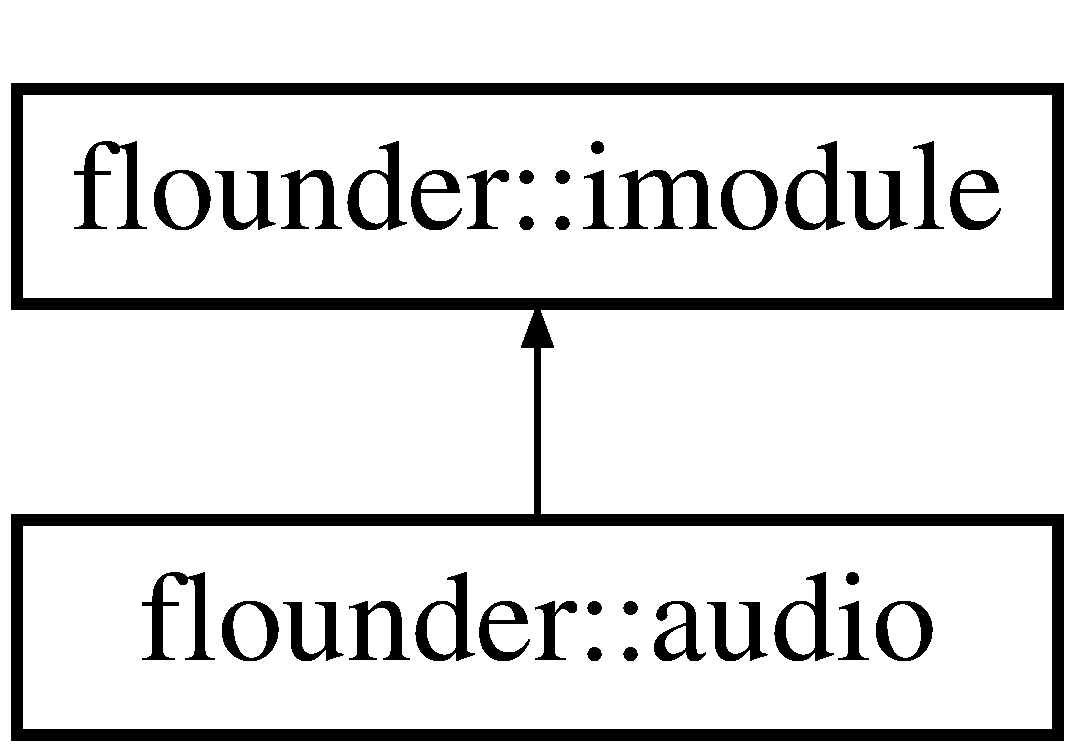
\includegraphics[height=2.000000cm]{classflounder_1_1audio}
\end{center}
\end{figure}
\subsection*{Public Member Functions}
\begin{DoxyCompactItemize}
\item 
\hyperlink{classflounder_1_1audio_a0aabbb226f542847145d89adb1144c16}{audio} ()
\begin{DoxyCompactList}\small\item\em Creates a new audio module. \end{DoxyCompactList}\item 
\hyperlink{classflounder_1_1audio_afb4d3bbb9ae399385a3abfe6e4e6d7ee}{$\sim$audio} ()
\begin{DoxyCompactList}\small\item\em Deconstructor for the audio module. \end{DoxyCompactList}\item 
void \hyperlink{classflounder_1_1audio_aabff6a1996b8571404023b6ac17009b6}{update} () override
\begin{DoxyCompactList}\small\item\em The update function for the module. \end{DoxyCompactList}\end{DoxyCompactItemize}
\subsection*{Static Public Member Functions}
\begin{DoxyCompactItemize}
\item 
static \hyperlink{classflounder_1_1audio}{audio} $\ast$ \hyperlink{classflounder_1_1audio_ac827774b8855e8a921ef9141c2515df8}{get} ()
\begin{DoxyCompactList}\small\item\em Gets this framework instance. \end{DoxyCompactList}\end{DoxyCompactItemize}
\subsection*{Private Attributes}
\begin{DoxyCompactItemize}
\item 
\mbox{\Hypertarget{classflounder_1_1audio_a6e577784668fbd39f2d6aa8e45bd2983}\label{classflounder_1_1audio_a6e577784668fbd39f2d6aa8e45bd2983}} 
A\+L\+Cdevice $\ast$ {\bfseries m\+\_\+device}
\item 
\mbox{\Hypertarget{classflounder_1_1audio_a361e675d6029769f9a366354a3e1cb61}\label{classflounder_1_1audio_a361e675d6029769f9a366354a3e1cb61}} 
A\+L\+Ccontext $\ast$ {\bfseries m\+\_\+context}
\item 
\mbox{\Hypertarget{classflounder_1_1audio_a58379153a6620d70633e20b4660502ea}\label{classflounder_1_1audio_a58379153a6620d70633e20b4660502ea}} 
int $\ast$ {\bfseries buffers}
\end{DoxyCompactItemize}


\subsection{Detailed Description}
A module used for loading, managing and playing a variety of different sound types. 



\subsection{Constructor \& Destructor Documentation}
\mbox{\Hypertarget{classflounder_1_1audio_a0aabbb226f542847145d89adb1144c16}\label{classflounder_1_1audio_a0aabbb226f542847145d89adb1144c16}} 
\index{flounder\+::audio@{flounder\+::audio}!audio@{audio}}
\index{audio@{audio}!flounder\+::audio@{flounder\+::audio}}
\subsubsection{\texorpdfstring{audio()}{audio()}}
{\footnotesize\ttfamily flounder\+::audio\+::audio (\begin{DoxyParamCaption}{ }\end{DoxyParamCaption})}



Creates a new audio module. 

\mbox{\Hypertarget{classflounder_1_1audio_afb4d3bbb9ae399385a3abfe6e4e6d7ee}\label{classflounder_1_1audio_afb4d3bbb9ae399385a3abfe6e4e6d7ee}} 
\index{flounder\+::audio@{flounder\+::audio}!````~audio@{$\sim$audio}}
\index{````~audio@{$\sim$audio}!flounder\+::audio@{flounder\+::audio}}
\subsubsection{\texorpdfstring{$\sim$audio()}{~audio()}}
{\footnotesize\ttfamily flounder\+::audio\+::$\sim$audio (\begin{DoxyParamCaption}{ }\end{DoxyParamCaption})}



Deconstructor for the audio module. 



\subsection{Member Function Documentation}
\mbox{\Hypertarget{classflounder_1_1audio_ac827774b8855e8a921ef9141c2515df8}\label{classflounder_1_1audio_ac827774b8855e8a921ef9141c2515df8}} 
\index{flounder\+::audio@{flounder\+::audio}!get@{get}}
\index{get@{get}!flounder\+::audio@{flounder\+::audio}}
\subsubsection{\texorpdfstring{get()}{get()}}
{\footnotesize\ttfamily static \hyperlink{classflounder_1_1audio}{audio}$\ast$ flounder\+::audio\+::get (\begin{DoxyParamCaption}{ }\end{DoxyParamCaption})\hspace{0.3cm}{\ttfamily [inline]}, {\ttfamily [static]}}



Gets this framework instance. 

\begin{DoxyReturn}{Returns}
The current module instance. 
\end{DoxyReturn}
\mbox{\Hypertarget{classflounder_1_1audio_aabff6a1996b8571404023b6ac17009b6}\label{classflounder_1_1audio_aabff6a1996b8571404023b6ac17009b6}} 
\index{flounder\+::audio@{flounder\+::audio}!update@{update}}
\index{update@{update}!flounder\+::audio@{flounder\+::audio}}
\subsubsection{\texorpdfstring{update()}{update()}}
{\footnotesize\ttfamily void flounder\+::audio\+::update (\begin{DoxyParamCaption}{ }\end{DoxyParamCaption})\hspace{0.3cm}{\ttfamily [override]}, {\ttfamily [virtual]}}



The update function for the module. 



Implements \hyperlink{classflounder_1_1imodule_a9a53d48a46b5f6b16a92b2cd8503f74a}{flounder\+::imodule}.



The documentation for this class was generated from the following files\+:\begin{DoxyCompactItemize}
\item 
Flounder-\/\+Core/src/devices/audio.\+h\item 
Flounder-\/\+Core/src/devices/audio.\+cpp\end{DoxyCompactItemize}

\hypertarget{classflounder_1_1axisbutton}{}\section{flounder\+:\+:axisbutton Class Reference}
\label{classflounder_1_1axisbutton}\index{flounder\+::axisbutton@{flounder\+::axisbutton}}


Axis composed of two buttons.  




{\ttfamily \#include $<$axisbutton.\+h$>$}

Inheritance diagram for flounder\+:\+:axisbutton\+:\begin{figure}[H]
\begin{center}
\leavevmode
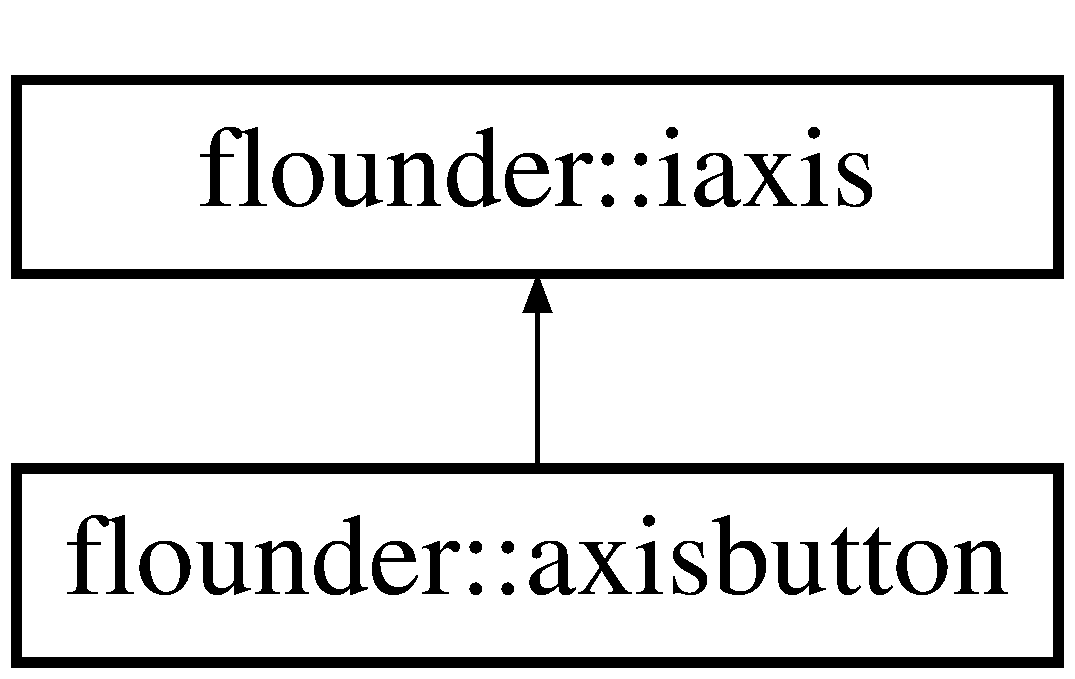
\includegraphics[height=2.000000cm]{classflounder_1_1axisbutton}
\end{center}
\end{figure}
\subsection*{Public Member Functions}
\begin{DoxyCompactItemize}
\item 
\hyperlink{classflounder_1_1axisbutton_a0f02ecccceb4155637ff3380335a0c62}{axisbutton} (\hyperlink{classflounder_1_1ibutton}{ibutton} $\ast$negative, \hyperlink{classflounder_1_1ibutton}{ibutton} $\ast$positive)
\begin{DoxyCompactList}\small\item\em Creates a new axis button. \end{DoxyCompactList}\item 
\hyperlink{classflounder_1_1axisbutton_a39d7d5faaf65ff5bef2cbded008762a9}{$\sim$axisbutton} ()
\begin{DoxyCompactList}\small\item\em Deconstructor for the axis joystick. \end{DoxyCompactList}\item 
float \hyperlink{classflounder_1_1axisbutton_aa5589f11ec6a9f4e6d01727903581539}{get\+Amount} () const override
\begin{DoxyCompactList}\small\item\em Gets the current value along the axis. -\/1 is smallest input, 1 is largest input. \end{DoxyCompactList}\end{DoxyCompactItemize}
\subsection*{Private Attributes}
\begin{DoxyCompactItemize}
\item 
\mbox{\Hypertarget{classflounder_1_1axisbutton_aaee98b4b372e3df4968bf1cdb22a7e76}\label{classflounder_1_1axisbutton_aaee98b4b372e3df4968bf1cdb22a7e76}} 
\hyperlink{classflounder_1_1ibutton}{ibutton} $\ast$ {\bfseries m\+\_\+negative}
\item 
\mbox{\Hypertarget{classflounder_1_1axisbutton_a4aa7adc6938d7ee7753d453a62f7f88e}\label{classflounder_1_1axisbutton_a4aa7adc6938d7ee7753d453a62f7f88e}} 
\hyperlink{classflounder_1_1ibutton}{ibutton} $\ast$ {\bfseries m\+\_\+positive}
\end{DoxyCompactItemize}


\subsection{Detailed Description}
Axis composed of two buttons. 



\subsection{Constructor \& Destructor Documentation}
\mbox{\Hypertarget{classflounder_1_1axisbutton_a0f02ecccceb4155637ff3380335a0c62}\label{classflounder_1_1axisbutton_a0f02ecccceb4155637ff3380335a0c62}} 
\index{flounder\+::axisbutton@{flounder\+::axisbutton}!axisbutton@{axisbutton}}
\index{axisbutton@{axisbutton}!flounder\+::axisbutton@{flounder\+::axisbutton}}
\subsubsection{\texorpdfstring{axisbutton()}{axisbutton()}}
{\footnotesize\ttfamily flounder\+::axisbutton\+::axisbutton (\begin{DoxyParamCaption}\item[{\hyperlink{classflounder_1_1ibutton}{ibutton} $\ast$}]{negative,  }\item[{\hyperlink{classflounder_1_1ibutton}{ibutton} $\ast$}]{positive }\end{DoxyParamCaption})}



Creates a new axis button. 


\begin{DoxyParams}{Parameters}
{\em negative} & When this button is down, the axis is negative. \\
\hline
{\em positive} & When this button is down, the axis is positive. \\
\hline
\end{DoxyParams}
\mbox{\Hypertarget{classflounder_1_1axisbutton_a39d7d5faaf65ff5bef2cbded008762a9}\label{classflounder_1_1axisbutton_a39d7d5faaf65ff5bef2cbded008762a9}} 
\index{flounder\+::axisbutton@{flounder\+::axisbutton}!````~axisbutton@{$\sim$axisbutton}}
\index{````~axisbutton@{$\sim$axisbutton}!flounder\+::axisbutton@{flounder\+::axisbutton}}
\subsubsection{\texorpdfstring{$\sim$axisbutton()}{~axisbutton()}}
{\footnotesize\ttfamily flounder\+::axisbutton\+::$\sim$axisbutton (\begin{DoxyParamCaption}{ }\end{DoxyParamCaption})}



Deconstructor for the axis joystick. 



\subsection{Member Function Documentation}
\mbox{\Hypertarget{classflounder_1_1axisbutton_aa5589f11ec6a9f4e6d01727903581539}\label{classflounder_1_1axisbutton_aa5589f11ec6a9f4e6d01727903581539}} 
\index{flounder\+::axisbutton@{flounder\+::axisbutton}!get\+Amount@{get\+Amount}}
\index{get\+Amount@{get\+Amount}!flounder\+::axisbutton@{flounder\+::axisbutton}}
\subsubsection{\texorpdfstring{get\+Amount()}{getAmount()}}
{\footnotesize\ttfamily float flounder\+::axisbutton\+::get\+Amount (\begin{DoxyParamCaption}{ }\end{DoxyParamCaption}) const\hspace{0.3cm}{\ttfamily [override]}, {\ttfamily [virtual]}}



Gets the current value along the axis. -\/1 is smallest input, 1 is largest input. 

\begin{DoxyReturn}{Returns}
The current value of the axis in the range (-\/1, 1). 
\end{DoxyReturn}


Implements \hyperlink{classflounder_1_1iaxis_a990ecb5ffa5ec07b3d5e2e4016b2e4a0}{flounder\+::iaxis}.



The documentation for this class was generated from the following files\+:\begin{DoxyCompactItemize}
\item 
Flounder-\/\+Core/src/inputs/axisbutton.\+h\item 
Flounder-\/\+Core/src/inputs/axisbutton.\+cpp\end{DoxyCompactItemize}

\hypertarget{classflounder_1_1axiscompound}{}\section{flounder\+:\+:axiscompound Class Reference}
\label{classflounder_1_1axiscompound}\index{flounder\+::axiscompound@{flounder\+::axiscompound}}


Axis composed of multiple other axes.  




{\ttfamily \#include $<$axiscompound.\+h$>$}

Inheritance diagram for flounder\+:\+:axiscompound\+:\begin{figure}[H]
\begin{center}
\leavevmode
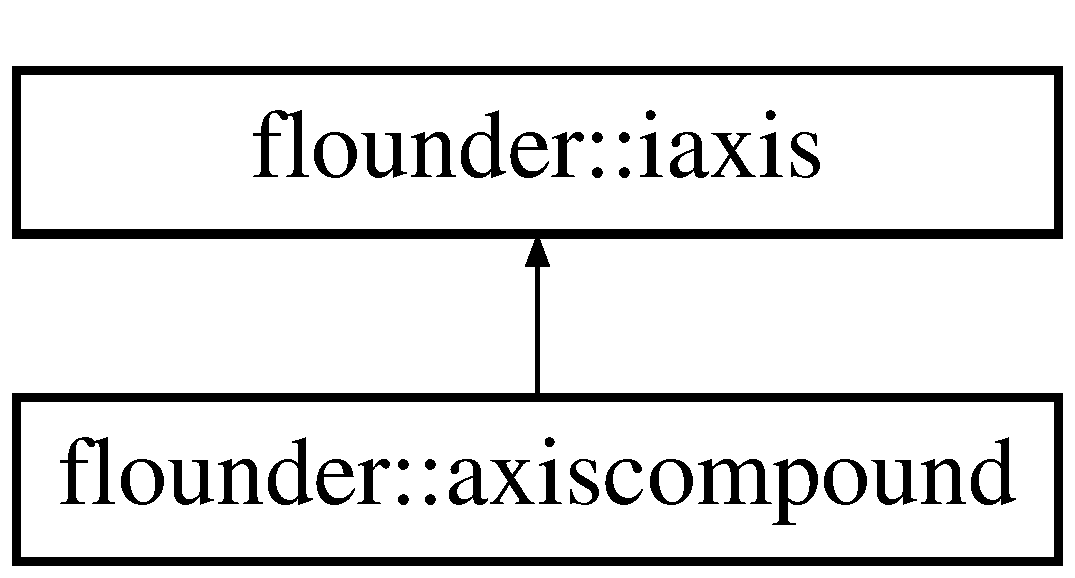
\includegraphics[height=2.000000cm]{classflounder_1_1axiscompound}
\end{center}
\end{figure}
\subsection*{Public Member Functions}
\begin{DoxyCompactItemize}
\item 
\hyperlink{classflounder_1_1axiscompound_a5f1704b50b966bca51730f7fecfc3728}{axiscompound} (const int n\+\_\+args,...)
\begin{DoxyCompactList}\small\item\em Creates a new compound axis. \end{DoxyCompactList}\item 
\hyperlink{classflounder_1_1axiscompound_ae6143bb6a584988c55aaa70545ffae91}{$\sim$axiscompound} ()
\begin{DoxyCompactList}\small\item\em Deconstructor for the compound axis. \end{DoxyCompactList}\item 
float \hyperlink{classflounder_1_1axiscompound_aad0f38f1a532c269cd0e803953861400}{get\+Amount} () const override
\begin{DoxyCompactList}\small\item\em Gets the current value along the axis. -\/1 is smallest input, 1 is largest input. \end{DoxyCompactList}\end{DoxyCompactItemize}
\subsection*{Private Attributes}
\begin{DoxyCompactItemize}
\item 
\mbox{\Hypertarget{classflounder_1_1axiscompound_ab876ccafbfabb22aac47b09ce4917b0c}\label{classflounder_1_1axiscompound_ab876ccafbfabb22aac47b09ce4917b0c}} 
int {\bfseries m\+\_\+count}
\item 
\mbox{\Hypertarget{classflounder_1_1axiscompound_a5bbc0ced9b75906a09ecfc327db4b42a}\label{classflounder_1_1axiscompound_a5bbc0ced9b75906a09ecfc327db4b42a}} 
\hyperlink{classflounder_1_1iaxis}{iaxis} $\ast$$\ast$ {\bfseries m\+\_\+axes}
\end{DoxyCompactItemize}


\subsection{Detailed Description}
Axis composed of multiple other axes. 



\subsection{Constructor \& Destructor Documentation}
\mbox{\Hypertarget{classflounder_1_1axiscompound_a5f1704b50b966bca51730f7fecfc3728}\label{classflounder_1_1axiscompound_a5f1704b50b966bca51730f7fecfc3728}} 
\index{flounder\+::axiscompound@{flounder\+::axiscompound}!axiscompound@{axiscompound}}
\index{axiscompound@{axiscompound}!flounder\+::axiscompound@{flounder\+::axiscompound}}
\subsubsection{\texorpdfstring{axiscompound()}{axiscompound()}}
{\footnotesize\ttfamily flounder\+::axiscompound\+::axiscompound (\begin{DoxyParamCaption}\item[{const int}]{n\+\_\+args,  }\item[{}]{... }\end{DoxyParamCaption})}



Creates a new compound axis. 


\begin{DoxyParams}{Parameters}
{\em n\+\_\+args} & The number of axes being added. \\
\hline
{\em ...} & The axes on the being added. \\
\hline
\end{DoxyParams}
\mbox{\Hypertarget{classflounder_1_1axiscompound_ae6143bb6a584988c55aaa70545ffae91}\label{classflounder_1_1axiscompound_ae6143bb6a584988c55aaa70545ffae91}} 
\index{flounder\+::axiscompound@{flounder\+::axiscompound}!````~axiscompound@{$\sim$axiscompound}}
\index{````~axiscompound@{$\sim$axiscompound}!flounder\+::axiscompound@{flounder\+::axiscompound}}
\subsubsection{\texorpdfstring{$\sim$axiscompound()}{~axiscompound()}}
{\footnotesize\ttfamily flounder\+::axiscompound\+::$\sim$axiscompound (\begin{DoxyParamCaption}{ }\end{DoxyParamCaption})}



Deconstructor for the compound axis. 



\subsection{Member Function Documentation}
\mbox{\Hypertarget{classflounder_1_1axiscompound_aad0f38f1a532c269cd0e803953861400}\label{classflounder_1_1axiscompound_aad0f38f1a532c269cd0e803953861400}} 
\index{flounder\+::axiscompound@{flounder\+::axiscompound}!get\+Amount@{get\+Amount}}
\index{get\+Amount@{get\+Amount}!flounder\+::axiscompound@{flounder\+::axiscompound}}
\subsubsection{\texorpdfstring{get\+Amount()}{getAmount()}}
{\footnotesize\ttfamily float flounder\+::axiscompound\+::get\+Amount (\begin{DoxyParamCaption}{ }\end{DoxyParamCaption}) const\hspace{0.3cm}{\ttfamily [override]}, {\ttfamily [virtual]}}



Gets the current value along the axis. -\/1 is smallest input, 1 is largest input. 

\begin{DoxyReturn}{Returns}
The current value of the axis in the range (-\/1, 1). 
\end{DoxyReturn}


Implements \hyperlink{classflounder_1_1iaxis_a990ecb5ffa5ec07b3d5e2e4016b2e4a0}{flounder\+::iaxis}.



The documentation for this class was generated from the following files\+:\begin{DoxyCompactItemize}
\item 
Flounder-\/\+Core/src/inputs/axiscompound.\+h\item 
Flounder-\/\+Core/src/inputs/axiscompound.\+cpp\end{DoxyCompactItemize}

\hypertarget{classflounder_1_1axisjoystick}{}\section{flounder\+:\+:axisjoystick Class Reference}
\label{classflounder_1_1axisjoystick}\index{flounder\+::axisjoystick@{flounder\+::axisjoystick}}


Axis from a joystick.  




{\ttfamily \#include $<$axisjoystick.\+h$>$}

Inheritance diagram for flounder\+:\+:axisjoystick\+:\begin{figure}[H]
\begin{center}
\leavevmode
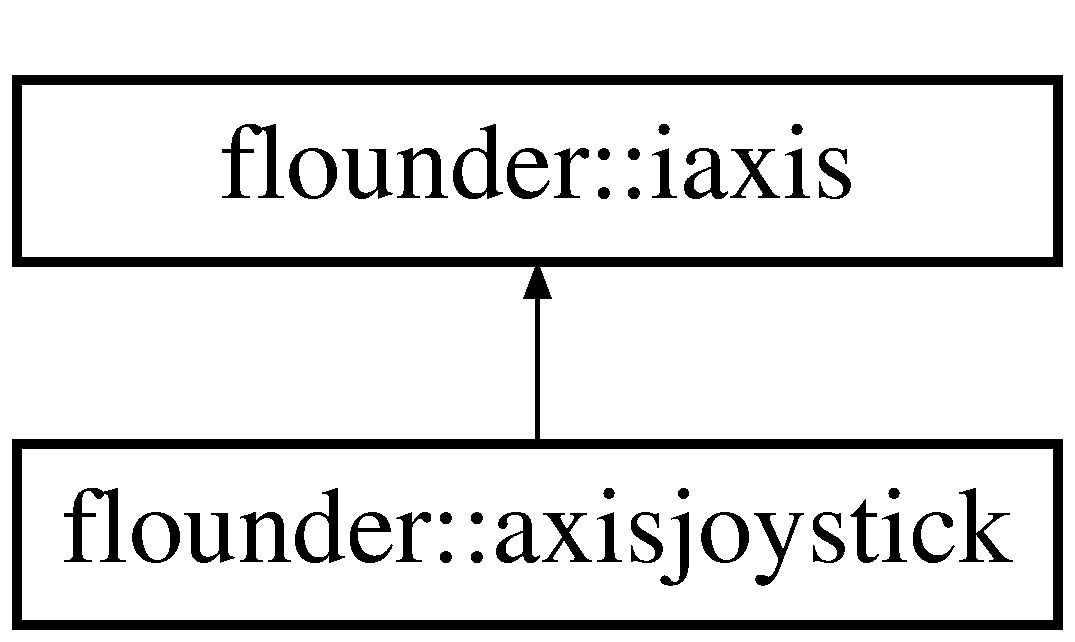
\includegraphics[height=2.000000cm]{classflounder_1_1axisjoystick}
\end{center}
\end{figure}
\subsection*{Public Member Functions}
\begin{DoxyCompactItemize}
\item 
\hyperlink{classflounder_1_1axisjoystick_a6415074e9ce0f9aae1d8071dc90a5f93}{axisjoystick} (const int \&joystick, const int n\+\_\+args,...)
\begin{DoxyCompactList}\small\item\em Creates a new axis joystick. \end{DoxyCompactList}\item 
\hyperlink{classflounder_1_1axisjoystick_aa006f728b79d1f0bd5101070782fcbb9}{$\sim$axisjoystick} ()
\begin{DoxyCompactList}\small\item\em Deconstructor for the axis joystick. \end{DoxyCompactList}\item 
float \hyperlink{classflounder_1_1axisjoystick_ae1c3dafedcb9458be0172e83f4197dac}{get\+Amount} () const override
\begin{DoxyCompactList}\small\item\em Gets the current value along the axis. -\/1 is smallest input, 1 is largest input. \end{DoxyCompactList}\end{DoxyCompactItemize}
\subsection*{Private Attributes}
\begin{DoxyCompactItemize}
\item 
\mbox{\Hypertarget{classflounder_1_1axisjoystick_a8107a9ae34c0ceb53d95efd7f5271db3}\label{classflounder_1_1axisjoystick_a8107a9ae34c0ceb53d95efd7f5271db3}} 
int {\bfseries m\+\_\+joystick}
\item 
\mbox{\Hypertarget{classflounder_1_1axisjoystick_a55c01fefa2832605ff86d610b67cc704}\label{classflounder_1_1axisjoystick_a55c01fefa2832605ff86d610b67cc704}} 
int {\bfseries m\+\_\+count}
\item 
\mbox{\Hypertarget{classflounder_1_1axisjoystick_aad5c6ca1cfef2ef2f525aa7d7ab76b9b}\label{classflounder_1_1axisjoystick_aad5c6ca1cfef2ef2f525aa7d7ab76b9b}} 
int $\ast$ {\bfseries m\+\_\+axes}
\end{DoxyCompactItemize}


\subsection{Detailed Description}
Axis from a joystick. 



\subsection{Constructor \& Destructor Documentation}
\mbox{\Hypertarget{classflounder_1_1axisjoystick_a6415074e9ce0f9aae1d8071dc90a5f93}\label{classflounder_1_1axisjoystick_a6415074e9ce0f9aae1d8071dc90a5f93}} 
\index{flounder\+::axisjoystick@{flounder\+::axisjoystick}!axisjoystick@{axisjoystick}}
\index{axisjoystick@{axisjoystick}!flounder\+::axisjoystick@{flounder\+::axisjoystick}}
\subsubsection{\texorpdfstring{axisjoystick()}{axisjoystick()}}
{\footnotesize\ttfamily flounder\+::axisjoystick\+::axisjoystick (\begin{DoxyParamCaption}\item[{const int \&}]{joystick,  }\item[{const int}]{n\+\_\+args,  }\item[{}]{... }\end{DoxyParamCaption})}



Creates a new axis joystick. 


\begin{DoxyParams}{Parameters}
{\em joystick} & The joystick. Should be one of the G\+L\+F\+W.\+J\+O\+Y\+S\+T\+I\+CK values. \\
\hline
{\em n\+\_\+args} & The number axes of joystick axes being checked. \\
\hline
{\em ...} & The axes on the joystick being checked. \\
\hline
\end{DoxyParams}
\mbox{\Hypertarget{classflounder_1_1axisjoystick_aa006f728b79d1f0bd5101070782fcbb9}\label{classflounder_1_1axisjoystick_aa006f728b79d1f0bd5101070782fcbb9}} 
\index{flounder\+::axisjoystick@{flounder\+::axisjoystick}!````~axisjoystick@{$\sim$axisjoystick}}
\index{````~axisjoystick@{$\sim$axisjoystick}!flounder\+::axisjoystick@{flounder\+::axisjoystick}}
\subsubsection{\texorpdfstring{$\sim$axisjoystick()}{~axisjoystick()}}
{\footnotesize\ttfamily flounder\+::axisjoystick\+::$\sim$axisjoystick (\begin{DoxyParamCaption}{ }\end{DoxyParamCaption})}



Deconstructor for the axis joystick. 



\subsection{Member Function Documentation}
\mbox{\Hypertarget{classflounder_1_1axisjoystick_ae1c3dafedcb9458be0172e83f4197dac}\label{classflounder_1_1axisjoystick_ae1c3dafedcb9458be0172e83f4197dac}} 
\index{flounder\+::axisjoystick@{flounder\+::axisjoystick}!get\+Amount@{get\+Amount}}
\index{get\+Amount@{get\+Amount}!flounder\+::axisjoystick@{flounder\+::axisjoystick}}
\subsubsection{\texorpdfstring{get\+Amount()}{getAmount()}}
{\footnotesize\ttfamily float flounder\+::axisjoystick\+::get\+Amount (\begin{DoxyParamCaption}{ }\end{DoxyParamCaption}) const\hspace{0.3cm}{\ttfamily [override]}, {\ttfamily [virtual]}}



Gets the current value along the axis. -\/1 is smallest input, 1 is largest input. 

\begin{DoxyReturn}{Returns}
The current value of the axis in the range (-\/1, 1). 
\end{DoxyReturn}


Implements \hyperlink{classflounder_1_1iaxis_a990ecb5ffa5ec07b3d5e2e4016b2e4a0}{flounder\+::iaxis}.



The documentation for this class was generated from the following files\+:\begin{DoxyCompactItemize}
\item 
Flounder-\/\+Core/src/inputs/axisjoystick.\+h\item 
Flounder-\/\+Core/src/inputs/axisjoystick.\+cpp\end{DoxyCompactItemize}

\hypertarget{classflounder_1_1buttoncompound}{}\section{flounder\+:\+:buttoncompound Class Reference}
\label{classflounder_1_1buttoncompound}\index{flounder\+::buttoncompound@{flounder\+::buttoncompound}}


Handles multiple buttons at once.  




{\ttfamily \#include $<$buttoncompound.\+h$>$}

Inheritance diagram for flounder\+:\+:buttoncompound\+:\begin{figure}[H]
\begin{center}
\leavevmode
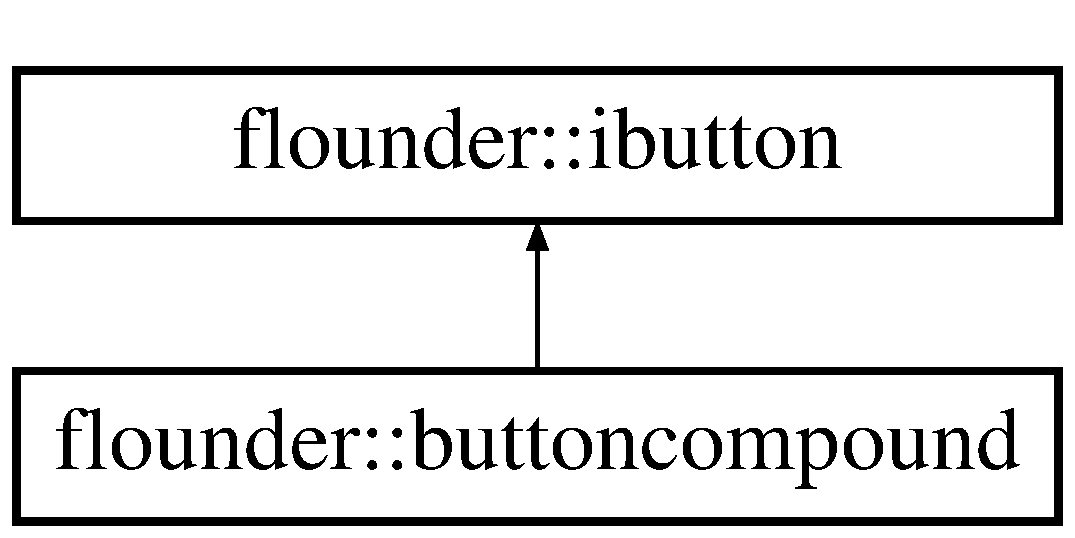
\includegraphics[height=2.000000cm]{classflounder_1_1buttoncompound}
\end{center}
\end{figure}
\subsection*{Public Member Functions}
\begin{DoxyCompactItemize}
\item 
\hyperlink{classflounder_1_1buttoncompound_a6fc9975e305663650b46f7034efab5af}{buttoncompound} (const int n\+\_\+args,...)
\begin{DoxyCompactList}\small\item\em Creates a new compound button. \end{DoxyCompactList}\item 
\hyperlink{classflounder_1_1buttoncompound_a6abb7a06910785964c92942e7ed00ef8}{$\sim$buttoncompound} ()
\begin{DoxyCompactList}\small\item\em Deconstructor for the compound button. \end{DoxyCompactList}\item 
bool \hyperlink{classflounder_1_1buttoncompound_a60ac6caaca37cd841c725259906a9196}{is\+Down} () const override
\begin{DoxyCompactList}\small\item\em Returns whether this button is currently pressed. \end{DoxyCompactList}\item 
bool \hyperlink{classflounder_1_1buttoncompound_ae14c6ee933dbc2550f16bc6307f20989}{was\+Down} () override
\begin{DoxyCompactList}\small\item\em Gets if the key is down and was not down before. Key press recognized as one click. \end{DoxyCompactList}\end{DoxyCompactItemize}
\subsection*{Private Attributes}
\begin{DoxyCompactItemize}
\item 
\mbox{\Hypertarget{classflounder_1_1buttoncompound_abd9fc2f19b8792e9086fa6d2e1ba99fc}\label{classflounder_1_1buttoncompound_abd9fc2f19b8792e9086fa6d2e1ba99fc}} 
int {\bfseries m\+\_\+count}
\item 
\mbox{\Hypertarget{classflounder_1_1buttoncompound_aaa087c79af2ceb2df78310ac780037f2}\label{classflounder_1_1buttoncompound_aaa087c79af2ceb2df78310ac780037f2}} 
\hyperlink{classflounder_1_1ibutton}{ibutton} $\ast$$\ast$ {\bfseries m\+\_\+buttons}
\item 
\mbox{\Hypertarget{classflounder_1_1buttoncompound_aeeefd0e962fb26c9ce781d87ebd74f12}\label{classflounder_1_1buttoncompound_aeeefd0e962fb26c9ce781d87ebd74f12}} 
bool {\bfseries m\+\_\+was\+Down}
\end{DoxyCompactItemize}


\subsection{Detailed Description}
Handles multiple buttons at once. 



\subsection{Constructor \& Destructor Documentation}
\mbox{\Hypertarget{classflounder_1_1buttoncompound_a6fc9975e305663650b46f7034efab5af}\label{classflounder_1_1buttoncompound_a6fc9975e305663650b46f7034efab5af}} 
\index{flounder\+::buttoncompound@{flounder\+::buttoncompound}!buttoncompound@{buttoncompound}}
\index{buttoncompound@{buttoncompound}!flounder\+::buttoncompound@{flounder\+::buttoncompound}}
\subsubsection{\texorpdfstring{buttoncompound()}{buttoncompound()}}
{\footnotesize\ttfamily flounder\+::buttoncompound\+::buttoncompound (\begin{DoxyParamCaption}\item[{const int}]{n\+\_\+args,  }\item[{}]{... }\end{DoxyParamCaption})}



Creates a new compound button. 


\begin{DoxyParams}{Parameters}
{\em n\+\_\+args} & The number buttons being added. \\
\hline
{\em ...} & The buttons on the being added. \\
\hline
\end{DoxyParams}
\mbox{\Hypertarget{classflounder_1_1buttoncompound_a6abb7a06910785964c92942e7ed00ef8}\label{classflounder_1_1buttoncompound_a6abb7a06910785964c92942e7ed00ef8}} 
\index{flounder\+::buttoncompound@{flounder\+::buttoncompound}!````~buttoncompound@{$\sim$buttoncompound}}
\index{````~buttoncompound@{$\sim$buttoncompound}!flounder\+::buttoncompound@{flounder\+::buttoncompound}}
\subsubsection{\texorpdfstring{$\sim$buttoncompound()}{~buttoncompound()}}
{\footnotesize\ttfamily flounder\+::buttoncompound\+::$\sim$buttoncompound (\begin{DoxyParamCaption}{ }\end{DoxyParamCaption})}



Deconstructor for the compound button. 



\subsection{Member Function Documentation}
\mbox{\Hypertarget{classflounder_1_1buttoncompound_a60ac6caaca37cd841c725259906a9196}\label{classflounder_1_1buttoncompound_a60ac6caaca37cd841c725259906a9196}} 
\index{flounder\+::buttoncompound@{flounder\+::buttoncompound}!is\+Down@{is\+Down}}
\index{is\+Down@{is\+Down}!flounder\+::buttoncompound@{flounder\+::buttoncompound}}
\subsubsection{\texorpdfstring{is\+Down()}{isDown()}}
{\footnotesize\ttfamily bool flounder\+::buttoncompound\+::is\+Down (\begin{DoxyParamCaption}{ }\end{DoxyParamCaption}) const\hspace{0.3cm}{\ttfamily [override]}, {\ttfamily [virtual]}}



Returns whether this button is currently pressed. 

\begin{DoxyReturn}{Returns}
True if the button is pressed, false otherwise. 
\end{DoxyReturn}


Implements \hyperlink{classflounder_1_1ibutton_af99b936d7329f74a27768ce6eb181327}{flounder\+::ibutton}.

\mbox{\Hypertarget{classflounder_1_1buttoncompound_ae14c6ee933dbc2550f16bc6307f20989}\label{classflounder_1_1buttoncompound_ae14c6ee933dbc2550f16bc6307f20989}} 
\index{flounder\+::buttoncompound@{flounder\+::buttoncompound}!was\+Down@{was\+Down}}
\index{was\+Down@{was\+Down}!flounder\+::buttoncompound@{flounder\+::buttoncompound}}
\subsubsection{\texorpdfstring{was\+Down()}{wasDown()}}
{\footnotesize\ttfamily bool flounder\+::buttoncompound\+::was\+Down (\begin{DoxyParamCaption}{ }\end{DoxyParamCaption})\hspace{0.3cm}{\ttfamily [override]}, {\ttfamily [virtual]}}



Gets if the key is down and was not down before. Key press recognized as one click. 

\begin{DoxyReturn}{Returns}
Is the key down and was not down before? 
\end{DoxyReturn}


Implements \hyperlink{classflounder_1_1ibutton_a5fb7b3493c0ea0e67bb9defc272da0d3}{flounder\+::ibutton}.



The documentation for this class was generated from the following files\+:\begin{DoxyCompactItemize}
\item 
Flounder-\/\+Core/src/inputs/buttoncompound.\+h\item 
Flounder-\/\+Core/src/inputs/buttoncompound.\+cpp\end{DoxyCompactItemize}

\hypertarget{classflounder_1_1buttonjoystick}{}\section{flounder\+:\+:buttonjoystick Class Reference}
\label{classflounder_1_1buttonjoystick}\index{flounder\+::buttonjoystick@{flounder\+::buttonjoystick}}


Button from a joystick.  




{\ttfamily \#include $<$buttonjoystick.\+h$>$}

Inheritance diagram for flounder\+:\+:buttonjoystick\+:\begin{figure}[H]
\begin{center}
\leavevmode
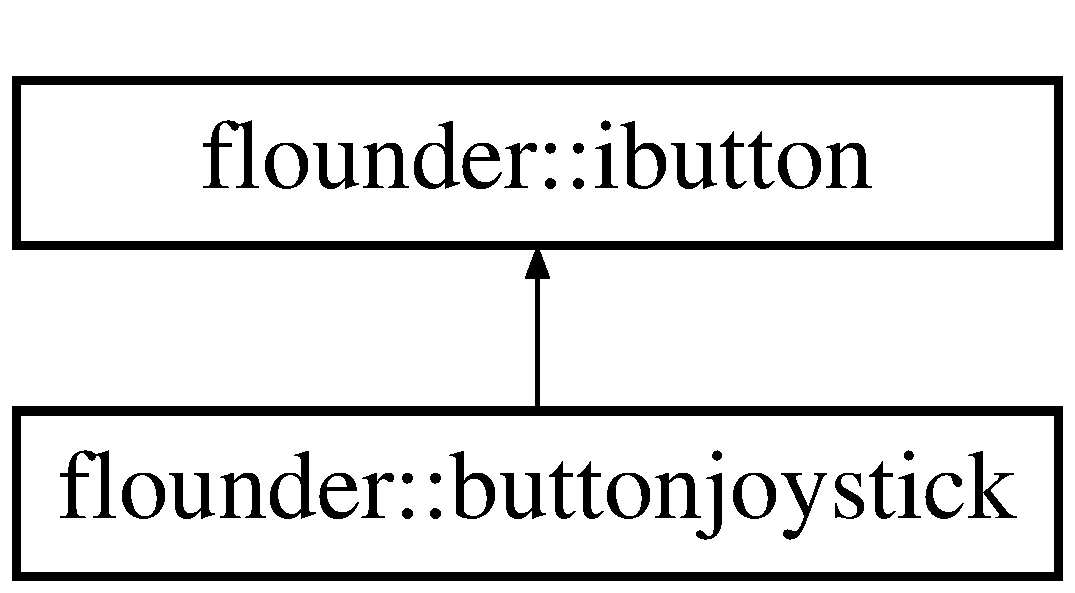
\includegraphics[height=2.000000cm]{classflounder_1_1buttonjoystick}
\end{center}
\end{figure}
\subsection*{Public Member Functions}
\begin{DoxyCompactItemize}
\item 
\hyperlink{classflounder_1_1buttonjoystick_a1b31996ff3588c033e85839aef2d35c8}{buttonjoystick} (const int \&joystick, const int n\+\_\+args,...)
\begin{DoxyCompactList}\small\item\em Creates a new button joystick. \end{DoxyCompactList}\item 
\hyperlink{classflounder_1_1buttonjoystick_aece2e8931c528cef0a266f17b2eba88b}{$\sim$buttonjoystick} ()
\begin{DoxyCompactList}\small\item\em Deconstructor for the button joystick. \end{DoxyCompactList}\item 
bool \hyperlink{classflounder_1_1buttonjoystick_ab6682d3554e007ef473c4595339f86f1}{is\+Down} () override
\begin{DoxyCompactList}\small\item\em Returns whether this button is currently pressed. \end{DoxyCompactList}\item 
bool \hyperlink{classflounder_1_1buttonjoystick_a99302b1345fa773ec839290ae6c406e7}{was\+Down} () override
\begin{DoxyCompactList}\small\item\em Gets if the key is down and was not down before. Key press recognized as one click. \end{DoxyCompactList}\end{DoxyCompactItemize}
\subsection*{Private Attributes}
\begin{DoxyCompactItemize}
\item 
\mbox{\Hypertarget{classflounder_1_1buttonjoystick_a3a6e21dff8b11ac6a58cfae4d33093ab}\label{classflounder_1_1buttonjoystick_a3a6e21dff8b11ac6a58cfae4d33093ab}} 
int {\bfseries m\+\_\+joystick}
\item 
\mbox{\Hypertarget{classflounder_1_1buttonjoystick_a2fa5decb08acdaf813707747bfccccd9}\label{classflounder_1_1buttonjoystick_a2fa5decb08acdaf813707747bfccccd9}} 
int {\bfseries m\+\_\+count}
\item 
\mbox{\Hypertarget{classflounder_1_1buttonjoystick_ad7f15d3fc515ec73cbbb755883c5dd0e}\label{classflounder_1_1buttonjoystick_ad7f15d3fc515ec73cbbb755883c5dd0e}} 
int $\ast$ {\bfseries m\+\_\+buttons}
\item 
\mbox{\Hypertarget{classflounder_1_1buttonjoystick_a2338ec61fb31f2299d7373faedf33d24}\label{classflounder_1_1buttonjoystick_a2338ec61fb31f2299d7373faedf33d24}} 
bool {\bfseries m\+\_\+was\+Down}
\end{DoxyCompactItemize}


\subsection{Detailed Description}
Button from a joystick. 



\subsection{Constructor \& Destructor Documentation}
\mbox{\Hypertarget{classflounder_1_1buttonjoystick_a1b31996ff3588c033e85839aef2d35c8}\label{classflounder_1_1buttonjoystick_a1b31996ff3588c033e85839aef2d35c8}} 
\index{flounder\+::buttonjoystick@{flounder\+::buttonjoystick}!buttonjoystick@{buttonjoystick}}
\index{buttonjoystick@{buttonjoystick}!flounder\+::buttonjoystick@{flounder\+::buttonjoystick}}
\subsubsection{\texorpdfstring{buttonjoystick()}{buttonjoystick()}}
{\footnotesize\ttfamily flounder\+::buttonjoystick\+::buttonjoystick (\begin{DoxyParamCaption}\item[{const int \&}]{joystick,  }\item[{const int}]{n\+\_\+args,  }\item[{}]{... }\end{DoxyParamCaption})\hspace{0.3cm}{\ttfamily [inline]}}



Creates a new button joystick. 


\begin{DoxyParams}{Parameters}
{\em joystick} & The joystick. Should be one of the G\+L\+F\+W.\+J\+O\+Y\+S\+T\+I\+CK values. \\
\hline
{\em n\+\_\+args} & The number buttons of joystick buttons being checked. \\
\hline
{\em ...} & The buttons on the joystick being checked. \\
\hline
\end{DoxyParams}
\mbox{\Hypertarget{classflounder_1_1buttonjoystick_aece2e8931c528cef0a266f17b2eba88b}\label{classflounder_1_1buttonjoystick_aece2e8931c528cef0a266f17b2eba88b}} 
\index{flounder\+::buttonjoystick@{flounder\+::buttonjoystick}!````~buttonjoystick@{$\sim$buttonjoystick}}
\index{````~buttonjoystick@{$\sim$buttonjoystick}!flounder\+::buttonjoystick@{flounder\+::buttonjoystick}}
\subsubsection{\texorpdfstring{$\sim$buttonjoystick()}{~buttonjoystick()}}
{\footnotesize\ttfamily flounder\+::buttonjoystick\+::$\sim$buttonjoystick (\begin{DoxyParamCaption}{ }\end{DoxyParamCaption})\hspace{0.3cm}{\ttfamily [inline]}}



Deconstructor for the button joystick. 



\subsection{Member Function Documentation}
\mbox{\Hypertarget{classflounder_1_1buttonjoystick_ab6682d3554e007ef473c4595339f86f1}\label{classflounder_1_1buttonjoystick_ab6682d3554e007ef473c4595339f86f1}} 
\index{flounder\+::buttonjoystick@{flounder\+::buttonjoystick}!is\+Down@{is\+Down}}
\index{is\+Down@{is\+Down}!flounder\+::buttonjoystick@{flounder\+::buttonjoystick}}
\subsubsection{\texorpdfstring{is\+Down()}{isDown()}}
{\footnotesize\ttfamily bool flounder\+::buttonjoystick\+::is\+Down (\begin{DoxyParamCaption}{ }\end{DoxyParamCaption})\hspace{0.3cm}{\ttfamily [inline]}, {\ttfamily [override]}, {\ttfamily [virtual]}}



Returns whether this button is currently pressed. 

\begin{DoxyReturn}{Returns}
True if the button is pressed, false otherwise. 
\end{DoxyReturn}


Implements \hyperlink{classflounder_1_1ibutton_ab64fd22a75ea66ce67fd9b1ad34fd837}{flounder\+::ibutton}.

\mbox{\Hypertarget{classflounder_1_1buttonjoystick_a99302b1345fa773ec839290ae6c406e7}\label{classflounder_1_1buttonjoystick_a99302b1345fa773ec839290ae6c406e7}} 
\index{flounder\+::buttonjoystick@{flounder\+::buttonjoystick}!was\+Down@{was\+Down}}
\index{was\+Down@{was\+Down}!flounder\+::buttonjoystick@{flounder\+::buttonjoystick}}
\subsubsection{\texorpdfstring{was\+Down()}{wasDown()}}
{\footnotesize\ttfamily bool flounder\+::buttonjoystick\+::was\+Down (\begin{DoxyParamCaption}{ }\end{DoxyParamCaption})\hspace{0.3cm}{\ttfamily [inline]}, {\ttfamily [override]}, {\ttfamily [virtual]}}



Gets if the key is down and was not down before. Key press recognized as one click. 

\begin{DoxyReturn}{Returns}
Is the key down and was not down before? 
\end{DoxyReturn}


Implements \hyperlink{classflounder_1_1ibutton_a5fb7b3493c0ea0e67bb9defc272da0d3}{flounder\+::ibutton}.



The documentation for this class was generated from the following file\+:\begin{DoxyCompactItemize}
\item 
C\+:/\+Users/mattp/\+Documents/\+Flounder/\+Flounder\+Core/\+Sources/inputs/buttonjoystick.\+h\end{DoxyCompactItemize}

\hypertarget{classflounder_1_1buttonkeyboard}{}\section{flounder\+:\+:buttonkeyboard Class Reference}
\label{classflounder_1_1buttonkeyboard}\index{flounder\+::buttonkeyboard@{flounder\+::buttonkeyboard}}


Keys from a keyboard.  




{\ttfamily \#include $<$buttonkeyboard.\+h$>$}

Inheritance diagram for flounder\+:\+:buttonkeyboard\+:\begin{figure}[H]
\begin{center}
\leavevmode
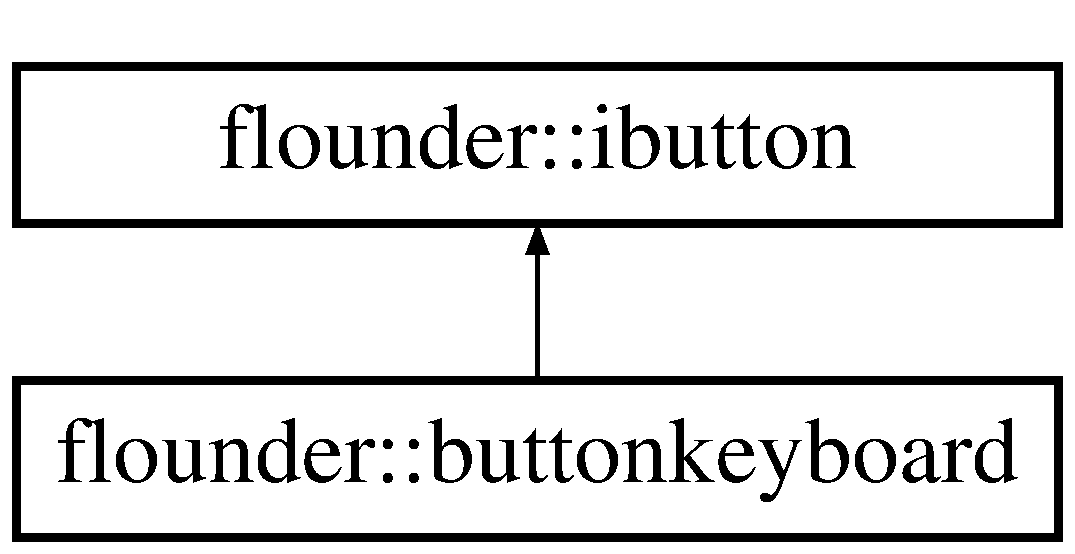
\includegraphics[height=2.000000cm]{classflounder_1_1buttonkeyboard}
\end{center}
\end{figure}
\subsection*{Public Member Functions}
\begin{DoxyCompactItemize}
\item 
\hyperlink{classflounder_1_1buttonkeyboard_a1cb133f346df9c1f0f401574bde868bc}{buttonkeyboard} (const int n\+\_\+args,...)
\begin{DoxyCompactList}\small\item\em Creates a new button keyboard. \end{DoxyCompactList}\item 
\hyperlink{classflounder_1_1buttonkeyboard_a76e965d16462442aaae33fe6fd2421ea}{$\sim$buttonkeyboard} ()
\begin{DoxyCompactList}\small\item\em Deconstructor for the button keyboard. \end{DoxyCompactList}\item 
bool \hyperlink{classflounder_1_1buttonkeyboard_a432555049251cec48431e4f14b6aa34b}{is\+Down} () override
\begin{DoxyCompactList}\small\item\em Returns whether this button is currently pressed. \end{DoxyCompactList}\item 
bool \hyperlink{classflounder_1_1buttonkeyboard_abc6b3c8cf9398f2a896408e390fd3a01}{was\+Down} () override
\begin{DoxyCompactList}\small\item\em Gets if the key is down and was not down before. Key press recognized as one click. \end{DoxyCompactList}\end{DoxyCompactItemize}
\subsection*{Private Attributes}
\begin{DoxyCompactItemize}
\item 
\mbox{\Hypertarget{classflounder_1_1buttonkeyboard_ac388d5c303d2bd2cddfc90853256d910}\label{classflounder_1_1buttonkeyboard_ac388d5c303d2bd2cddfc90853256d910}} 
int {\bfseries m\+\_\+count}
\item 
\mbox{\Hypertarget{classflounder_1_1buttonkeyboard_a6347baab78a95b15c0c54c3d65355fde}\label{classflounder_1_1buttonkeyboard_a6347baab78a95b15c0c54c3d65355fde}} 
int $\ast$ {\bfseries m\+\_\+keys}
\item 
\mbox{\Hypertarget{classflounder_1_1buttonkeyboard_a0d8fc28fc7e8293fa401a0b048dc26b6}\label{classflounder_1_1buttonkeyboard_a0d8fc28fc7e8293fa401a0b048dc26b6}} 
bool {\bfseries m\+\_\+was\+Down}
\end{DoxyCompactItemize}


\subsection{Detailed Description}
Keys from a keyboard. 



\subsection{Constructor \& Destructor Documentation}
\mbox{\Hypertarget{classflounder_1_1buttonkeyboard_a1cb133f346df9c1f0f401574bde868bc}\label{classflounder_1_1buttonkeyboard_a1cb133f346df9c1f0f401574bde868bc}} 
\index{flounder\+::buttonkeyboard@{flounder\+::buttonkeyboard}!buttonkeyboard@{buttonkeyboard}}
\index{buttonkeyboard@{buttonkeyboard}!flounder\+::buttonkeyboard@{flounder\+::buttonkeyboard}}
\subsubsection{\texorpdfstring{buttonkeyboard()}{buttonkeyboard()}}
{\footnotesize\ttfamily flounder\+::buttonkeyboard\+::buttonkeyboard (\begin{DoxyParamCaption}\item[{const int}]{n\+\_\+args,  }\item[{}]{... }\end{DoxyParamCaption})\hspace{0.3cm}{\ttfamily [inline]}}



Creates a new button keyboard. 


\begin{DoxyParams}{Parameters}
{\em n\+\_\+args} & The number keys of keyboard buttons being checked. \\
\hline
{\em ...} & The keys on the keyboard being checked. \\
\hline
\end{DoxyParams}
\mbox{\Hypertarget{classflounder_1_1buttonkeyboard_a76e965d16462442aaae33fe6fd2421ea}\label{classflounder_1_1buttonkeyboard_a76e965d16462442aaae33fe6fd2421ea}} 
\index{flounder\+::buttonkeyboard@{flounder\+::buttonkeyboard}!````~buttonkeyboard@{$\sim$buttonkeyboard}}
\index{````~buttonkeyboard@{$\sim$buttonkeyboard}!flounder\+::buttonkeyboard@{flounder\+::buttonkeyboard}}
\subsubsection{\texorpdfstring{$\sim$buttonkeyboard()}{~buttonkeyboard()}}
{\footnotesize\ttfamily flounder\+::buttonkeyboard\+::$\sim$buttonkeyboard (\begin{DoxyParamCaption}{ }\end{DoxyParamCaption})\hspace{0.3cm}{\ttfamily [inline]}}



Deconstructor for the button keyboard. 



\subsection{Member Function Documentation}
\mbox{\Hypertarget{classflounder_1_1buttonkeyboard_a432555049251cec48431e4f14b6aa34b}\label{classflounder_1_1buttonkeyboard_a432555049251cec48431e4f14b6aa34b}} 
\index{flounder\+::buttonkeyboard@{flounder\+::buttonkeyboard}!is\+Down@{is\+Down}}
\index{is\+Down@{is\+Down}!flounder\+::buttonkeyboard@{flounder\+::buttonkeyboard}}
\subsubsection{\texorpdfstring{is\+Down()}{isDown()}}
{\footnotesize\ttfamily bool flounder\+::buttonkeyboard\+::is\+Down (\begin{DoxyParamCaption}{ }\end{DoxyParamCaption})\hspace{0.3cm}{\ttfamily [inline]}, {\ttfamily [override]}, {\ttfamily [virtual]}}



Returns whether this button is currently pressed. 

\begin{DoxyReturn}{Returns}
True if the button is pressed, false otherwise. 
\end{DoxyReturn}


Implements \hyperlink{classflounder_1_1ibutton_ab64fd22a75ea66ce67fd9b1ad34fd837}{flounder\+::ibutton}.

\mbox{\Hypertarget{classflounder_1_1buttonkeyboard_abc6b3c8cf9398f2a896408e390fd3a01}\label{classflounder_1_1buttonkeyboard_abc6b3c8cf9398f2a896408e390fd3a01}} 
\index{flounder\+::buttonkeyboard@{flounder\+::buttonkeyboard}!was\+Down@{was\+Down}}
\index{was\+Down@{was\+Down}!flounder\+::buttonkeyboard@{flounder\+::buttonkeyboard}}
\subsubsection{\texorpdfstring{was\+Down()}{wasDown()}}
{\footnotesize\ttfamily bool flounder\+::buttonkeyboard\+::was\+Down (\begin{DoxyParamCaption}{ }\end{DoxyParamCaption})\hspace{0.3cm}{\ttfamily [inline]}, {\ttfamily [override]}, {\ttfamily [virtual]}}



Gets if the key is down and was not down before. Key press recognized as one click. 

\begin{DoxyReturn}{Returns}
Is the key down and was not down before? 
\end{DoxyReturn}


Implements \hyperlink{classflounder_1_1ibutton_a5fb7b3493c0ea0e67bb9defc272da0d3}{flounder\+::ibutton}.



The documentation for this class was generated from the following file\+:\begin{DoxyCompactItemize}
\item 
C\+:/\+Users/mattp/\+Documents/\+Flounder/\+Flounder\+Core/\+Sources/inputs/buttonkeyboard.\+h\end{DoxyCompactItemize}

\hypertarget{classflounder_1_1buttonmouse}{}\section{flounder\+:\+:buttonmouse Class Reference}
\label{classflounder_1_1buttonmouse}\index{flounder\+::buttonmouse@{flounder\+::buttonmouse}}


Button from a mouse.  




{\ttfamily \#include $<$buttonmouse.\+h$>$}

Inheritance diagram for flounder\+:\+:buttonmouse\+:\begin{figure}[H]
\begin{center}
\leavevmode
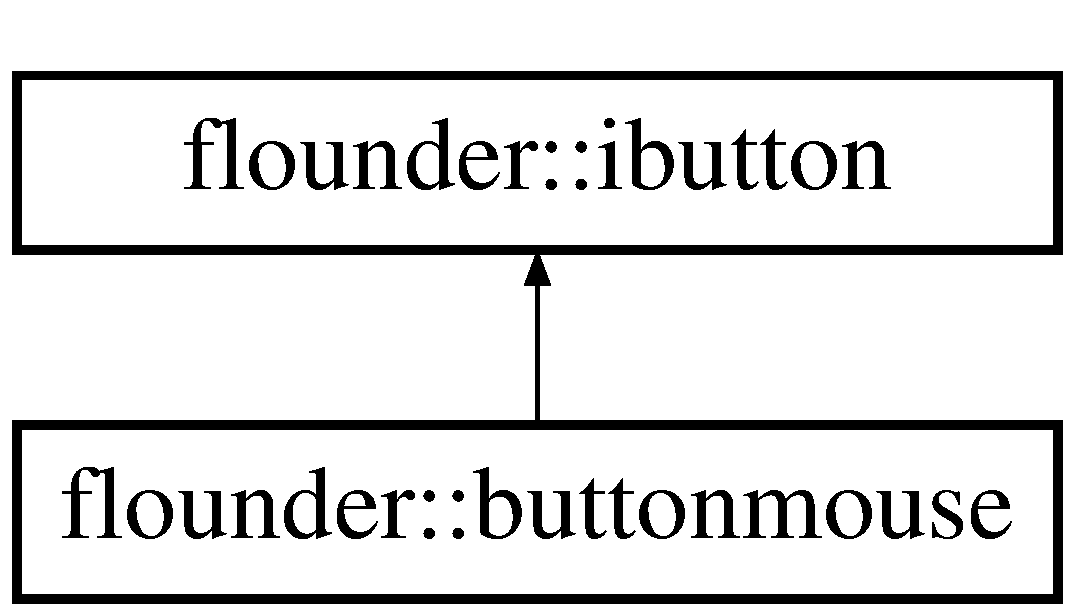
\includegraphics[height=2.000000cm]{classflounder_1_1buttonmouse}
\end{center}
\end{figure}
\subsection*{Public Member Functions}
\begin{DoxyCompactItemize}
\item 
\hyperlink{classflounder_1_1buttonmouse_a6721eb42c25bc50c2a4db56ca27c4cda}{buttonmouse} (const int n\+\_\+args,...)
\begin{DoxyCompactList}\small\item\em Creates a new button mouse. \end{DoxyCompactList}\item 
\hyperlink{classflounder_1_1buttonmouse_aa967f7f977040b0f4a58dc10d4414e75}{$\sim$buttonmouse} ()
\begin{DoxyCompactList}\small\item\em Deconstructor for the button mouse. \end{DoxyCompactList}\item 
bool \hyperlink{classflounder_1_1buttonmouse_ab4d7ecd54f144f03886b5ef467666be1}{is\+Down} () override
\begin{DoxyCompactList}\small\item\em Returns whether this button is currently pressed. \end{DoxyCompactList}\item 
bool \hyperlink{classflounder_1_1buttonmouse_a7dad01481ebb01755db054a0acbc8159}{was\+Down} () override
\begin{DoxyCompactList}\small\item\em Gets if the key is down and was not down before. Key press recognized as one click. \end{DoxyCompactList}\end{DoxyCompactItemize}
\subsection*{Private Attributes}
\begin{DoxyCompactItemize}
\item 
\mbox{\Hypertarget{classflounder_1_1buttonmouse_abedc20e1fc3ccc65a4e0c64ebe801935}\label{classflounder_1_1buttonmouse_abedc20e1fc3ccc65a4e0c64ebe801935}} 
int {\bfseries m\+\_\+count}
\item 
\mbox{\Hypertarget{classflounder_1_1buttonmouse_a8e520120c157797cfe59c267eac13689}\label{classflounder_1_1buttonmouse_a8e520120c157797cfe59c267eac13689}} 
int $\ast$ {\bfseries m\+\_\+buttons}
\item 
\mbox{\Hypertarget{classflounder_1_1buttonmouse_aa65460a6d76ece35fd264bc7a5185b47}\label{classflounder_1_1buttonmouse_aa65460a6d76ece35fd264bc7a5185b47}} 
bool {\bfseries m\+\_\+was\+Down}
\end{DoxyCompactItemize}


\subsection{Detailed Description}
Button from a mouse. 



\subsection{Constructor \& Destructor Documentation}
\mbox{\Hypertarget{classflounder_1_1buttonmouse_a6721eb42c25bc50c2a4db56ca27c4cda}\label{classflounder_1_1buttonmouse_a6721eb42c25bc50c2a4db56ca27c4cda}} 
\index{flounder\+::buttonmouse@{flounder\+::buttonmouse}!buttonmouse@{buttonmouse}}
\index{buttonmouse@{buttonmouse}!flounder\+::buttonmouse@{flounder\+::buttonmouse}}
\subsubsection{\texorpdfstring{buttonmouse()}{buttonmouse()}}
{\footnotesize\ttfamily flounder\+::buttonmouse\+::buttonmouse (\begin{DoxyParamCaption}\item[{const int}]{n\+\_\+args,  }\item[{}]{... }\end{DoxyParamCaption})\hspace{0.3cm}{\ttfamily [inline]}}



Creates a new button mouse. 


\begin{DoxyParams}{Parameters}
{\em n\+\_\+args} & The number buttons of mouse buttons being checked. \\
\hline
{\em ...} & The buttons on the mouse being checked. \\
\hline
\end{DoxyParams}
\mbox{\Hypertarget{classflounder_1_1buttonmouse_aa967f7f977040b0f4a58dc10d4414e75}\label{classflounder_1_1buttonmouse_aa967f7f977040b0f4a58dc10d4414e75}} 
\index{flounder\+::buttonmouse@{flounder\+::buttonmouse}!````~buttonmouse@{$\sim$buttonmouse}}
\index{````~buttonmouse@{$\sim$buttonmouse}!flounder\+::buttonmouse@{flounder\+::buttonmouse}}
\subsubsection{\texorpdfstring{$\sim$buttonmouse()}{~buttonmouse()}}
{\footnotesize\ttfamily flounder\+::buttonmouse\+::$\sim$buttonmouse (\begin{DoxyParamCaption}{ }\end{DoxyParamCaption})\hspace{0.3cm}{\ttfamily [inline]}}



Deconstructor for the button mouse. 



\subsection{Member Function Documentation}
\mbox{\Hypertarget{classflounder_1_1buttonmouse_ab4d7ecd54f144f03886b5ef467666be1}\label{classflounder_1_1buttonmouse_ab4d7ecd54f144f03886b5ef467666be1}} 
\index{flounder\+::buttonmouse@{flounder\+::buttonmouse}!is\+Down@{is\+Down}}
\index{is\+Down@{is\+Down}!flounder\+::buttonmouse@{flounder\+::buttonmouse}}
\subsubsection{\texorpdfstring{is\+Down()}{isDown()}}
{\footnotesize\ttfamily bool flounder\+::buttonmouse\+::is\+Down (\begin{DoxyParamCaption}{ }\end{DoxyParamCaption})\hspace{0.3cm}{\ttfamily [inline]}, {\ttfamily [override]}, {\ttfamily [virtual]}}



Returns whether this button is currently pressed. 

\begin{DoxyReturn}{Returns}
True if the button is pressed, false otherwise. 
\end{DoxyReturn}


Implements \hyperlink{classflounder_1_1ibutton_ab64fd22a75ea66ce67fd9b1ad34fd837}{flounder\+::ibutton}.

\mbox{\Hypertarget{classflounder_1_1buttonmouse_a7dad01481ebb01755db054a0acbc8159}\label{classflounder_1_1buttonmouse_a7dad01481ebb01755db054a0acbc8159}} 
\index{flounder\+::buttonmouse@{flounder\+::buttonmouse}!was\+Down@{was\+Down}}
\index{was\+Down@{was\+Down}!flounder\+::buttonmouse@{flounder\+::buttonmouse}}
\subsubsection{\texorpdfstring{was\+Down()}{wasDown()}}
{\footnotesize\ttfamily bool flounder\+::buttonmouse\+::was\+Down (\begin{DoxyParamCaption}{ }\end{DoxyParamCaption})\hspace{0.3cm}{\ttfamily [inline]}, {\ttfamily [override]}, {\ttfamily [virtual]}}



Gets if the key is down and was not down before. Key press recognized as one click. 

\begin{DoxyReturn}{Returns}
Is the key down and was not down before? 
\end{DoxyReturn}


Implements \hyperlink{classflounder_1_1ibutton_a5fb7b3493c0ea0e67bb9defc272da0d3}{flounder\+::ibutton}.



The documentation for this class was generated from the following file\+:\begin{DoxyCompactItemize}
\item 
C\+:/\+Users/mattp/\+Documents/\+Flounder/\+Flounder\+Core/\+Sources/inputs/buttonmouse.\+h\end{DoxyCompactItemize}

\hypertarget{classflounder_1_1camera}{}\section{flounder\+:\+:camera Class Reference}
\label{classflounder_1_1camera}\index{flounder\+::camera@{flounder\+::camera}}


A module used for managing cameras in 2D and 3D worlds.  




{\ttfamily \#include $<$camera.\+h$>$}

Inheritance diagram for flounder\+:\+:camera\+:\begin{figure}[H]
\begin{center}
\leavevmode
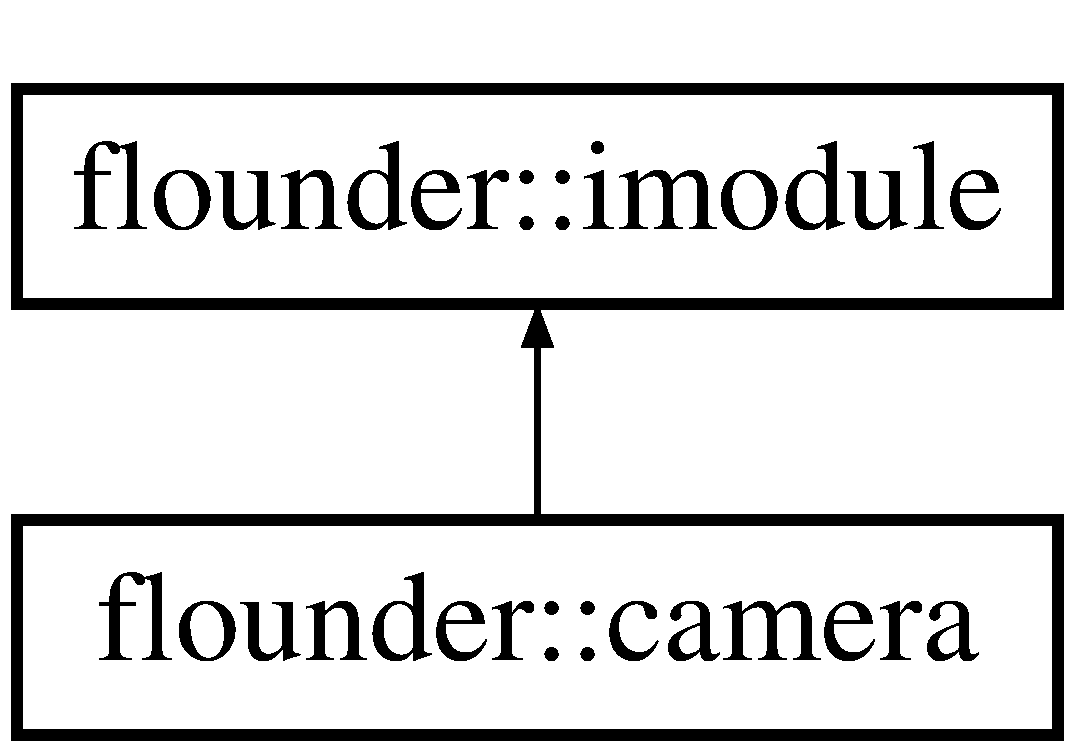
\includegraphics[height=2.000000cm]{classflounder_1_1camera}
\end{center}
\end{figure}
\subsection*{Public Member Functions}
\begin{DoxyCompactItemize}
\item 
\hyperlink{classflounder_1_1camera_a84e93f21953c21facbcddf77d83c7c47}{camera} ()
\begin{DoxyCompactList}\small\item\em Creates a new camera module. \end{DoxyCompactList}\item 
\hyperlink{classflounder_1_1camera_ada55d236f9f9b9a301b3fd747d15d4d0}{$\sim$camera} ()
\begin{DoxyCompactList}\small\item\em Deconstructor for the camera module. \end{DoxyCompactList}\item 
void \hyperlink{classflounder_1_1camera_a6b2da3a1c348764d3cf954db5ac5b357}{update} () override
\begin{DoxyCompactList}\small\item\em The update function for the module. \end{DoxyCompactList}\item 
\hyperlink{classflounder_1_1icamera}{icamera} $\ast$ \hyperlink{classflounder_1_1camera_abc16dba0c44428f99ce65af2c1dac5b8}{get\+Camera} ()
\begin{DoxyCompactList}\small\item\em Gets the current camera object. \end{DoxyCompactList}\item 
void \hyperlink{classflounder_1_1camera_a43117513a5beffafb902448843206a79}{set\+Camera} (\hyperlink{classflounder_1_1icamera}{icamera} $\ast$\hyperlink{classflounder_1_1camera}{camera})
\begin{DoxyCompactList}\small\item\em Sets the current camera to a new camera. \end{DoxyCompactList}\item 
\hyperlink{classflounder_1_1iplayer}{iplayer} $\ast$ \hyperlink{classflounder_1_1camera_a662d47759c3b570def49a75981b95bc4}{get\+Player} ()
\begin{DoxyCompactList}\small\item\em Gets the current player object. \end{DoxyCompactList}\item 
void \hyperlink{classflounder_1_1camera_aa572fb3c1428b8a69aba9e9944405c5c}{set\+Player} (\hyperlink{classflounder_1_1iplayer}{iplayer} $\ast$player)
\begin{DoxyCompactList}\small\item\em Sets the current player to a new player. \end{DoxyCompactList}\end{DoxyCompactItemize}
\subsection*{Static Public Member Functions}
\begin{DoxyCompactItemize}
\item 
static \hyperlink{classflounder_1_1camera}{camera} $\ast$ \hyperlink{classflounder_1_1camera_a3ea117d355e4925fa5238bae5e6e46b1}{get} ()
\begin{DoxyCompactList}\small\item\em Gets this framework instance. \end{DoxyCompactList}\end{DoxyCompactItemize}
\subsection*{Private Attributes}
\begin{DoxyCompactItemize}
\item 
\mbox{\Hypertarget{classflounder_1_1camera_a0fdfccdc761a7c057c431e2e1b1e9456}\label{classflounder_1_1camera_a0fdfccdc761a7c057c431e2e1b1e9456}} 
\hyperlink{classflounder_1_1icamera}{icamera} $\ast$ {\bfseries m\+\_\+camera}
\item 
\mbox{\Hypertarget{classflounder_1_1camera_a8dc046728d790d77234a25dca96ac649}\label{classflounder_1_1camera_a8dc046728d790d77234a25dca96ac649}} 
\hyperlink{classflounder_1_1iplayer}{iplayer} $\ast$ {\bfseries m\+\_\+player}
\end{DoxyCompactItemize}


\subsection{Detailed Description}
A module used for managing cameras in 2D and 3D worlds. 



\subsection{Constructor \& Destructor Documentation}
\mbox{\Hypertarget{classflounder_1_1camera_a84e93f21953c21facbcddf77d83c7c47}\label{classflounder_1_1camera_a84e93f21953c21facbcddf77d83c7c47}} 
\index{flounder\+::camera@{flounder\+::camera}!camera@{camera}}
\index{camera@{camera}!flounder\+::camera@{flounder\+::camera}}
\subsubsection{\texorpdfstring{camera()}{camera()}}
{\footnotesize\ttfamily flounder\+::camera\+::camera (\begin{DoxyParamCaption}{ }\end{DoxyParamCaption})}



Creates a new camera module. 

\mbox{\Hypertarget{classflounder_1_1camera_ada55d236f9f9b9a301b3fd747d15d4d0}\label{classflounder_1_1camera_ada55d236f9f9b9a301b3fd747d15d4d0}} 
\index{flounder\+::camera@{flounder\+::camera}!````~camera@{$\sim$camera}}
\index{````~camera@{$\sim$camera}!flounder\+::camera@{flounder\+::camera}}
\subsubsection{\texorpdfstring{$\sim$camera()}{~camera()}}
{\footnotesize\ttfamily flounder\+::camera\+::$\sim$camera (\begin{DoxyParamCaption}{ }\end{DoxyParamCaption})}



Deconstructor for the camera module. 



\subsection{Member Function Documentation}
\mbox{\Hypertarget{classflounder_1_1camera_a3ea117d355e4925fa5238bae5e6e46b1}\label{classflounder_1_1camera_a3ea117d355e4925fa5238bae5e6e46b1}} 
\index{flounder\+::camera@{flounder\+::camera}!get@{get}}
\index{get@{get}!flounder\+::camera@{flounder\+::camera}}
\subsubsection{\texorpdfstring{get()}{get()}}
{\footnotesize\ttfamily static \hyperlink{classflounder_1_1camera}{camera}$\ast$ flounder\+::camera\+::get (\begin{DoxyParamCaption}{ }\end{DoxyParamCaption})\hspace{0.3cm}{\ttfamily [inline]}, {\ttfamily [static]}}



Gets this framework instance. 

\begin{DoxyReturn}{Returns}
The current module instance. 
\end{DoxyReturn}
\mbox{\Hypertarget{classflounder_1_1camera_abc16dba0c44428f99ce65af2c1dac5b8}\label{classflounder_1_1camera_abc16dba0c44428f99ce65af2c1dac5b8}} 
\index{flounder\+::camera@{flounder\+::camera}!get\+Camera@{get\+Camera}}
\index{get\+Camera@{get\+Camera}!flounder\+::camera@{flounder\+::camera}}
\subsubsection{\texorpdfstring{get\+Camera()}{getCamera()}}
{\footnotesize\ttfamily \hyperlink{classflounder_1_1icamera}{icamera}$\ast$ flounder\+::camera\+::get\+Camera (\begin{DoxyParamCaption}{ }\end{DoxyParamCaption})\hspace{0.3cm}{\ttfamily [inline]}}



Gets the current camera object. 

\begin{DoxyReturn}{Returns}
The current camera. 
\end{DoxyReturn}
\mbox{\Hypertarget{classflounder_1_1camera_a662d47759c3b570def49a75981b95bc4}\label{classflounder_1_1camera_a662d47759c3b570def49a75981b95bc4}} 
\index{flounder\+::camera@{flounder\+::camera}!get\+Player@{get\+Player}}
\index{get\+Player@{get\+Player}!flounder\+::camera@{flounder\+::camera}}
\subsubsection{\texorpdfstring{get\+Player()}{getPlayer()}}
{\footnotesize\ttfamily \hyperlink{classflounder_1_1iplayer}{iplayer}$\ast$ flounder\+::camera\+::get\+Player (\begin{DoxyParamCaption}{ }\end{DoxyParamCaption})\hspace{0.3cm}{\ttfamily [inline]}}



Gets the current player object. 

\begin{DoxyReturn}{Returns}
The current player. 
\end{DoxyReturn}
\mbox{\Hypertarget{classflounder_1_1camera_a43117513a5beffafb902448843206a79}\label{classflounder_1_1camera_a43117513a5beffafb902448843206a79}} 
\index{flounder\+::camera@{flounder\+::camera}!set\+Camera@{set\+Camera}}
\index{set\+Camera@{set\+Camera}!flounder\+::camera@{flounder\+::camera}}
\subsubsection{\texorpdfstring{set\+Camera()}{setCamera()}}
{\footnotesize\ttfamily void flounder\+::camera\+::set\+Camera (\begin{DoxyParamCaption}\item[{\hyperlink{classflounder_1_1icamera}{icamera} $\ast$}]{camera }\end{DoxyParamCaption})\hspace{0.3cm}{\ttfamily [inline]}}



Sets the current camera to a new camera. 


\begin{DoxyParams}{Parameters}
{\em camera} & The new camera. \\
\hline
\end{DoxyParams}
\mbox{\Hypertarget{classflounder_1_1camera_aa572fb3c1428b8a69aba9e9944405c5c}\label{classflounder_1_1camera_aa572fb3c1428b8a69aba9e9944405c5c}} 
\index{flounder\+::camera@{flounder\+::camera}!set\+Player@{set\+Player}}
\index{set\+Player@{set\+Player}!flounder\+::camera@{flounder\+::camera}}
\subsubsection{\texorpdfstring{set\+Player()}{setPlayer()}}
{\footnotesize\ttfamily void flounder\+::camera\+::set\+Player (\begin{DoxyParamCaption}\item[{\hyperlink{classflounder_1_1iplayer}{iplayer} $\ast$}]{player }\end{DoxyParamCaption})\hspace{0.3cm}{\ttfamily [inline]}}



Sets the current player to a new player. 


\begin{DoxyParams}{Parameters}
{\em player} & The new player. \\
\hline
\end{DoxyParams}
\mbox{\Hypertarget{classflounder_1_1camera_a6b2da3a1c348764d3cf954db5ac5b357}\label{classflounder_1_1camera_a6b2da3a1c348764d3cf954db5ac5b357}} 
\index{flounder\+::camera@{flounder\+::camera}!update@{update}}
\index{update@{update}!flounder\+::camera@{flounder\+::camera}}
\subsubsection{\texorpdfstring{update()}{update()}}
{\footnotesize\ttfamily void flounder\+::camera\+::update (\begin{DoxyParamCaption}{ }\end{DoxyParamCaption})\hspace{0.3cm}{\ttfamily [override]}, {\ttfamily [virtual]}}



The update function for the module. 



Implements \hyperlink{classflounder_1_1imodule_a9a53d48a46b5f6b16a92b2cd8503f74a}{flounder\+::imodule}.



The documentation for this class was generated from the following files\+:\begin{DoxyCompactItemize}
\item 
Flounder-\/\+Core/src/camera/camera.\+h\item 
Flounder-\/\+Core/src/camera/camera.\+cpp\end{DoxyCompactItemize}

\hypertarget{classflounder_1_1character}{}\section{flounder\+:\+:character Class Reference}
\label{classflounder_1_1character}\index{flounder\+::character@{flounder\+::character}}


Simple data structure class holding information about a certain glyph in the font texture atlas. All sizes are for a font-\/size of 1.  




{\ttfamily \#include $<$character.\+h$>$}

\subsection*{Public Member Functions}
\begin{DoxyCompactItemize}
\item 
\hyperlink{classflounder_1_1character_ae258dfe0dc5ac451346ceca6b0ff6647}{character} (const int \&id, const double \&texture\+CoordX, const double \&texture\+CoordY, const double \&texure\+SizeX, const double \&texure\+SizeY, const double \&offsetX, const double \&offsetY, const double \&sizeX, const double \&sizeY, const double \&advanceX)
\begin{DoxyCompactList}\small\item\em Creates a new character. \end{DoxyCompactList}\item 
\hyperlink{classflounder_1_1character_a0d67c2d619b0f138c54381428df5a32e}{$\sim$character} ()
\begin{DoxyCompactList}\small\item\em Deconstructor for the character. \end{DoxyCompactList}\item 
\mbox{\Hypertarget{classflounder_1_1character_ae42232768011b10cc7866f9981cd9b95}\label{classflounder_1_1character_ae42232768011b10cc7866f9981cd9b95}} 
int {\bfseries get\+Id} () const
\item 
\mbox{\Hypertarget{classflounder_1_1character_ad63d095d8b23b48c1a3844bfcbf8f599}\label{classflounder_1_1character_ad63d095d8b23b48c1a3844bfcbf8f599}} 
double {\bfseries get\+Texture\+CoordX} () const
\item 
\mbox{\Hypertarget{classflounder_1_1character_acc080516b920d2004439926e04f4c9dd}\label{classflounder_1_1character_acc080516b920d2004439926e04f4c9dd}} 
double {\bfseries get\+Texture\+CoordY} () const
\item 
\mbox{\Hypertarget{classflounder_1_1character_adbb2dfc7795d330b95c94c1b59882df7}\label{classflounder_1_1character_adbb2dfc7795d330b95c94c1b59882df7}} 
double {\bfseries get\+Max\+Texture\+CoordX} () const
\item 
\mbox{\Hypertarget{classflounder_1_1character_aa3bb4c6e1e080b33558187ce152d01da}\label{classflounder_1_1character_aa3bb4c6e1e080b33558187ce152d01da}} 
double {\bfseries get\+Max\+Texture\+CoordY} () const
\item 
\mbox{\Hypertarget{classflounder_1_1character_a71d7519a0f746d1594544782dc300cd9}\label{classflounder_1_1character_a71d7519a0f746d1594544782dc300cd9}} 
double {\bfseries get\+OffsetX} () const
\item 
\mbox{\Hypertarget{classflounder_1_1character_af814c678bdb4daf7144cce8872c539b2}\label{classflounder_1_1character_af814c678bdb4daf7144cce8872c539b2}} 
double {\bfseries get\+OffsetY} () const
\item 
\mbox{\Hypertarget{classflounder_1_1character_a0a7197d6203b4b7cbf79b96d52b41015}\label{classflounder_1_1character_a0a7197d6203b4b7cbf79b96d52b41015}} 
double {\bfseries get\+SizeX} () const
\item 
\mbox{\Hypertarget{classflounder_1_1character_aadee37791914443e8a1e17a621ab08d8}\label{classflounder_1_1character_aadee37791914443e8a1e17a621ab08d8}} 
double {\bfseries get\+SizeY} () const
\item 
\mbox{\Hypertarget{classflounder_1_1character_a6ee097f0940f2de06d263b4c7415137f}\label{classflounder_1_1character_a6ee097f0940f2de06d263b4c7415137f}} 
double {\bfseries get\+AdvanceX} () const
\end{DoxyCompactItemize}
\subsection*{Private Attributes}
\begin{DoxyCompactItemize}
\item 
\mbox{\Hypertarget{classflounder_1_1character_abb280f071ad1d88797fdea541ac902bd}\label{classflounder_1_1character_abb280f071ad1d88797fdea541ac902bd}} 
int {\bfseries m\+\_\+id}
\item 
\mbox{\Hypertarget{classflounder_1_1character_a05d4b071a3e5ada68462834c4770c5d3}\label{classflounder_1_1character_a05d4b071a3e5ada68462834c4770c5d3}} 
double {\bfseries m\+\_\+texture\+CoordX}
\item 
\mbox{\Hypertarget{classflounder_1_1character_adb63d0e79f51d4e3b72b8fa2d5267cc2}\label{classflounder_1_1character_adb63d0e79f51d4e3b72b8fa2d5267cc2}} 
double {\bfseries m\+\_\+texture\+CoordY}
\item 
\mbox{\Hypertarget{classflounder_1_1character_ae66ecc7b0ae8329ab00e3c5425be4650}\label{classflounder_1_1character_ae66ecc7b0ae8329ab00e3c5425be4650}} 
double {\bfseries m\+\_\+max\+Texture\+CoordX}
\item 
\mbox{\Hypertarget{classflounder_1_1character_a0d45d1b5b061b1ad92bfa0dfcb8d8eb3}\label{classflounder_1_1character_a0d45d1b5b061b1ad92bfa0dfcb8d8eb3}} 
double {\bfseries m\+\_\+max\+Texture\+CoordY}
\item 
\mbox{\Hypertarget{classflounder_1_1character_a8fc09cc216a225e682bae81bda4e8cf3}\label{classflounder_1_1character_a8fc09cc216a225e682bae81bda4e8cf3}} 
double {\bfseries m\+\_\+offsetX}
\item 
\mbox{\Hypertarget{classflounder_1_1character_a3a9fe9ce66a993dc378c959838c9c395}\label{classflounder_1_1character_a3a9fe9ce66a993dc378c959838c9c395}} 
double {\bfseries m\+\_\+offsetY}
\item 
\mbox{\Hypertarget{classflounder_1_1character_a85401b05cebbae9683f9e612b42b2019}\label{classflounder_1_1character_a85401b05cebbae9683f9e612b42b2019}} 
double {\bfseries m\+\_\+sizeX}
\item 
\mbox{\Hypertarget{classflounder_1_1character_a64700822c775e92782274369607ff3ca}\label{classflounder_1_1character_a64700822c775e92782274369607ff3ca}} 
double {\bfseries m\+\_\+sizeY}
\item 
\mbox{\Hypertarget{classflounder_1_1character_a7a317fd9bb7b6e2c601d60b65b08a935}\label{classflounder_1_1character_a7a317fd9bb7b6e2c601d60b65b08a935}} 
double {\bfseries m\+\_\+advanceX}
\end{DoxyCompactItemize}


\subsection{Detailed Description}
Simple data structure class holding information about a certain glyph in the font texture atlas. All sizes are for a font-\/size of 1. 



\subsection{Constructor \& Destructor Documentation}
\mbox{\Hypertarget{classflounder_1_1character_ae258dfe0dc5ac451346ceca6b0ff6647}\label{classflounder_1_1character_ae258dfe0dc5ac451346ceca6b0ff6647}} 
\index{flounder\+::character@{flounder\+::character}!character@{character}}
\index{character@{character}!flounder\+::character@{flounder\+::character}}
\subsubsection{\texorpdfstring{character()}{character()}}
{\footnotesize\ttfamily flounder\+::character\+::character (\begin{DoxyParamCaption}\item[{const int \&}]{id,  }\item[{const double \&}]{texture\+CoordX,  }\item[{const double \&}]{texture\+CoordY,  }\item[{const double \&}]{texure\+SizeX,  }\item[{const double \&}]{texure\+SizeY,  }\item[{const double \&}]{offsetX,  }\item[{const double \&}]{offsetY,  }\item[{const double \&}]{sizeX,  }\item[{const double \&}]{sizeY,  }\item[{const double \&}]{advanceX }\end{DoxyParamCaption})}



Creates a new character. 


\begin{DoxyParams}{Parameters}
{\em id} & The A\+S\+C\+II value of the character. \\
\hline
{\em texture\+CoordX} & The x texture coordinate for the top left corner of the character in the texture atlas. \\
\hline
{\em texture\+CoordY} & The y texture coordinate for the top left corner of the character in the texture atlas. \\
\hline
{\em texure\+SizeX} & The width of the character in the texture atlas. \\
\hline
{\em texure\+SizeY} & The height of the character in the texture atlas. \\
\hline
{\em offsetX} & The x distance from the cursor to the left edge of the character\textquotesingle{}s quad. \\
\hline
{\em offsetY} & The y distance from the cursor to the top edge of the character\textquotesingle{}s quad. \\
\hline
{\em sizeX} & The width of the character\textquotesingle{}s quad in screen space. \\
\hline
{\em sizeY} & The height of the character\textquotesingle{}s quad in screen space. \\
\hline
{\em advanceX} & How far in pixels the cursor should advance after adding this character. \\
\hline
\end{DoxyParams}
\mbox{\Hypertarget{classflounder_1_1character_a0d67c2d619b0f138c54381428df5a32e}\label{classflounder_1_1character_a0d67c2d619b0f138c54381428df5a32e}} 
\index{flounder\+::character@{flounder\+::character}!````~character@{$\sim$character}}
\index{````~character@{$\sim$character}!flounder\+::character@{flounder\+::character}}
\subsubsection{\texorpdfstring{$\sim$character()}{~character()}}
{\footnotesize\ttfamily flounder\+::character\+::$\sim$character (\begin{DoxyParamCaption}{ }\end{DoxyParamCaption})}



Deconstructor for the character. 



The documentation for this class was generated from the following files\+:\begin{DoxyCompactItemize}
\item 
Flounder-\/\+Core/src/fonts/character.\+h\item 
Flounder-\/\+Core/src/fonts/character.\+cpp\end{DoxyCompactItemize}

\hypertarget{structchunk}{}\section{chunk Struct Reference}
\label{structchunk}\index{chunk@{chunk}}
\subsection*{Public Attributes}
\begin{DoxyCompactItemize}
\item 
\mbox{\Hypertarget{structchunk_a0b5cc0c5a9b91945c42373db2a499fb1}\label{structchunk_a0b5cc0c5a9b91945c42373db2a499fb1}} 
uint32 {\bfseries length}
\item 
\mbox{\Hypertarget{structchunk_a05d5489f3807bc7ba149c1904241d087}\label{structchunk_a05d5489f3807bc7ba149c1904241d087}} 
uint32 {\bfseries type}
\end{DoxyCompactItemize}


The documentation for this struct was generated from the following file\+:\begin{DoxyCompactItemize}
\item 
C\+:/\+Users/mattp/\+Documents/\+Flounder/\+Flounder\+Core/\+Sources/textures/stb\+\_\+image.\+c\end{DoxyCompactItemize}

\hypertarget{classflounder_1_1colour}{}\section{flounder\+:\+:colour Class Reference}
\label{classflounder_1_1colour}\index{flounder\+::colour@{flounder\+::colour}}


Holds a R\+G\+BA colour.  




{\ttfamily \#include $<$colour.\+h$>$}

\subsection*{Public Member Functions}
\begin{DoxyCompactItemize}
\item 
\hyperlink{classflounder_1_1colour_a63a24979006e1472ae81c1be0d62f2cc}{colour} ()
\begin{DoxyCompactList}\small\item\em Constructor for colour. \end{DoxyCompactList}\item 
\hyperlink{classflounder_1_1colour_a398f40f90e10ec7d9ee9e6ce71147eca}{colour} (const float \&r, const float \&g, const float \&b)
\begin{DoxyCompactList}\small\item\em Constructor for colour. \end{DoxyCompactList}\item 
\hyperlink{classflounder_1_1colour_a0c27be9e6510b2449f38d7b4e839ca84}{colour} (const float \&r, const float \&g, const float \&b, const bool \&convert)
\begin{DoxyCompactList}\small\item\em Constructor for colour. \end{DoxyCompactList}\item 
\hyperlink{classflounder_1_1colour_a6c90f6f71418a734bfc3cd09eaf7f9f4}{colour} (const float \&r, const float \&g, const float \&b, const float \&a)
\begin{DoxyCompactList}\small\item\em Constructor for colour. \end{DoxyCompactList}\item 
\hyperlink{classflounder_1_1colour_a7c72f8a01847dd1221acfad5f2f83173}{colour} (const float \&r, const float \&g, const float \&b, const float \&a, const bool \&convert)
\begin{DoxyCompactList}\small\item\em Constructor for colour. \end{DoxyCompactList}\item 
\hyperlink{classflounder_1_1colour_ad13a6e7245e03a49474958afaa174025}{colour} (const \hyperlink{classflounder_1_1colour}{colour} \&source)
\begin{DoxyCompactList}\small\item\em Constructor for colour. \end{DoxyCompactList}\item 
\hyperlink{classflounder_1_1colour_ab2ccda8311376ec5a54243b1e9c5c694}{$\sim$colour} ()
\begin{DoxyCompactList}\small\item\em Deconstructor for colour. \end{DoxyCompactList}\item 
\hyperlink{classflounder_1_1colour}{colour} $\ast$ \hyperlink{classflounder_1_1colour_a2dad1722e39dd03a51b59ccab45035e2}{set} (const float \&r, const float \&g, const float \&b)
\begin{DoxyCompactList}\small\item\em Sets values in the colour. \end{DoxyCompactList}\item 
\hyperlink{classflounder_1_1colour}{colour} $\ast$ \hyperlink{classflounder_1_1colour_ad33c2b45456403221e46c980c07c3994}{set} (const float \&r, const float \&g, const float \&b, const bool \&convert)
\begin{DoxyCompactList}\small\item\em Sets values in the colour. \end{DoxyCompactList}\item 
\hyperlink{classflounder_1_1colour}{colour} $\ast$ \hyperlink{classflounder_1_1colour_a3f3c46b24810827cda5949ce813258a9}{set} (const float \&r, const float \&g, const float \&b, const float \&a)
\begin{DoxyCompactList}\small\item\em Sets values in the colour. \end{DoxyCompactList}\item 
\hyperlink{classflounder_1_1colour}{colour} $\ast$ \hyperlink{classflounder_1_1colour_af6f72267ba0dfbf4235bd820103249e7}{set} (const float \&r, const float \&g, const float \&b, const float \&a, const bool \&convert)
\begin{DoxyCompactList}\small\item\em Sets values in the colour. \end{DoxyCompactList}\item 
\hyperlink{classflounder_1_1colour}{colour} $\ast$ \hyperlink{classflounder_1_1colour_a7fabd96bd7baa0aaa398e7f55aa6db81}{set} (const \hyperlink{classflounder_1_1colour}{colour} \&source)
\begin{DoxyCompactList}\small\item\em Sets values in the colour. \end{DoxyCompactList}\item 
\hyperlink{classflounder_1_1colour}{colour} $\ast$ \hyperlink{classflounder_1_1colour_ae60ded359183b2669720e40139e291a7}{scale} (const float scalar)
\begin{DoxyCompactList}\small\item\em Scales the colour by a scalar. \end{DoxyCompactList}\item 
\mbox{\Hypertarget{classflounder_1_1colour_a0ead3d1f80571522cace5158a77b4184}\label{classflounder_1_1colour_a0ead3d1f80571522cace5158a77b4184}} 
float \hyperlink{classflounder_1_1colour_a0ead3d1f80571522cace5158a77b4184}{length} ()
\begin{DoxyCompactList}\small\item\em \begin{DoxyReturn}{Returns}
The length of the colour. 
\end{DoxyReturn}
\end{DoxyCompactList}\item 
\mbox{\Hypertarget{classflounder_1_1colour_aa3c91c3000ec427f64fa2162418ca6fe}\label{classflounder_1_1colour_aa3c91c3000ec427f64fa2162418ca6fe}} 
float \hyperlink{classflounder_1_1colour_aa3c91c3000ec427f64fa2162418ca6fe}{length\+Squared} ()
\begin{DoxyCompactList}\small\item\em \begin{DoxyReturn}{Returns}
The length squared of the colour. 
\end{DoxyReturn}
\end{DoxyCompactList}\end{DoxyCompactItemize}
\subsection*{Static Public Member Functions}
\begin{DoxyCompactItemize}
\item 
static \hyperlink{classflounder_1_1colour}{colour} $\ast$ \hyperlink{classflounder_1_1colour_a5d9f9d26b93a5414bdfc62b7526dca70}{add} (const \hyperlink{classflounder_1_1colour}{colour} \&left, const \hyperlink{classflounder_1_1colour}{colour} \&right, \hyperlink{classflounder_1_1colour}{colour} $\ast$destination)
\begin{DoxyCompactList}\small\item\em Adds two colours together and places the result in the destination colour. \end{DoxyCompactList}\item 
static \hyperlink{classflounder_1_1colour}{colour} $\ast$ \hyperlink{classflounder_1_1colour_a081a20a1be566ff1317d4214ef60f33d}{subtract} (const \hyperlink{classflounder_1_1colour}{colour} \&left, const \hyperlink{classflounder_1_1colour}{colour} \&right, \hyperlink{classflounder_1_1colour}{colour} $\ast$destination)
\begin{DoxyCompactList}\small\item\em Subtracts two colours together and places the result in the destination colour. \end{DoxyCompactList}\item 
static \hyperlink{classflounder_1_1colour}{colour} $\ast$ \hyperlink{classflounder_1_1colour_ada2598a03766be3adad831e17dcd822a}{multiply} (const \hyperlink{classflounder_1_1colour}{colour} \&left, const \hyperlink{classflounder_1_1colour}{colour} \&right, \hyperlink{classflounder_1_1colour}{colour} $\ast$destination)
\begin{DoxyCompactList}\small\item\em Multiplies two colours together and places the result in the destination colour. \end{DoxyCompactList}\item 
static \hyperlink{classflounder_1_1colour}{colour} $\ast$ \hyperlink{classflounder_1_1colour_afcbab734ed7ee0c3927ac0473150ed2a}{divide} (const \hyperlink{classflounder_1_1colour}{colour} \&left, const \hyperlink{classflounder_1_1colour}{colour} \&right, \hyperlink{classflounder_1_1colour}{colour} $\ast$destination)
\begin{DoxyCompactList}\small\item\em Divides two colours together and places the result in the destination colour. \end{DoxyCompactList}\item 
static \hyperlink{classflounder_1_1colour}{colour} $\ast$ \hyperlink{classflounder_1_1colour_a28e6e41406cd96df4d956a2c963fd767}{interpolate} (const \hyperlink{classflounder_1_1colour}{colour} \&left, const \hyperlink{classflounder_1_1colour}{colour} \&right, float blend, \hyperlink{classflounder_1_1colour}{colour} $\ast$destination)
\begin{DoxyCompactList}\small\item\em Interpolates between two colours and places the result in the destination colour. \end{DoxyCompactList}\item 
static \hyperlink{classflounder_1_1colour}{colour} $\ast$ \hyperlink{classflounder_1_1colour_a3f9e4ec638e7e240d86704d821d0c3bc}{get\+Unit} (const \hyperlink{classflounder_1_1colour}{colour} \&source, \hyperlink{classflounder_1_1colour}{colour} $\ast$destination)
\begin{DoxyCompactList}\small\item\em Gets a colour representing the unit value of this colour. \end{DoxyCompactList}\item 
static float \hyperlink{classflounder_1_1colour_adb8aba4ecd184a4fbdf04261db788096}{length} (const \hyperlink{classflounder_1_1colour}{colour} \&source)
\begin{DoxyCompactList}\small\item\em Gets the length of the colour. \end{DoxyCompactList}\item 
static float \hyperlink{classflounder_1_1colour_a9eae1aa8bda5bec5c914edfc4f077057}{length\+Squared} (const \hyperlink{classflounder_1_1colour}{colour} \&source)
\begin{DoxyCompactList}\small\item\em Gets the length squared of the colour. \end{DoxyCompactList}\end{DoxyCompactItemize}
\subsection*{Public Attributes}
\begin{DoxyCompactItemize}
\item 
\mbox{\Hypertarget{classflounder_1_1colour_ab143424eb7da34ce697c17b99be6079a}\label{classflounder_1_1colour_ab143424eb7da34ce697c17b99be6079a}} 
float {\bfseries r}
\item 
\mbox{\Hypertarget{classflounder_1_1colour_a15f34b3519639333763844da1fd58199}\label{classflounder_1_1colour_a15f34b3519639333763844da1fd58199}} 
float {\bfseries g}
\item 
\mbox{\Hypertarget{classflounder_1_1colour_a8a4f0ed5abf283a4d1fd7c4e00dc9c4d}\label{classflounder_1_1colour_a8a4f0ed5abf283a4d1fd7c4e00dc9c4d}} 
float {\bfseries b}
\item 
\mbox{\Hypertarget{classflounder_1_1colour_ab51885f0cf9043ad626cd7e4abd04b07}\label{classflounder_1_1colour_ab51885f0cf9043ad626cd7e4abd04b07}} 
float {\bfseries a}
\end{DoxyCompactItemize}


\subsection{Detailed Description}
Holds a R\+G\+BA colour. 



\subsection{Constructor \& Destructor Documentation}
\mbox{\Hypertarget{classflounder_1_1colour_a63a24979006e1472ae81c1be0d62f2cc}\label{classflounder_1_1colour_a63a24979006e1472ae81c1be0d62f2cc}} 
\index{flounder\+::colour@{flounder\+::colour}!colour@{colour}}
\index{colour@{colour}!flounder\+::colour@{flounder\+::colour}}
\subsubsection{\texorpdfstring{colour()}{colour()}\hspace{0.1cm}{\footnotesize\ttfamily [1/6]}}
{\footnotesize\ttfamily flounder\+::colour\+::colour (\begin{DoxyParamCaption}{ }\end{DoxyParamCaption})}



Constructor for colour. 

\mbox{\Hypertarget{classflounder_1_1colour_a398f40f90e10ec7d9ee9e6ce71147eca}\label{classflounder_1_1colour_a398f40f90e10ec7d9ee9e6ce71147eca}} 
\index{flounder\+::colour@{flounder\+::colour}!colour@{colour}}
\index{colour@{colour}!flounder\+::colour@{flounder\+::colour}}
\subsubsection{\texorpdfstring{colour()}{colour()}\hspace{0.1cm}{\footnotesize\ttfamily [2/6]}}
{\footnotesize\ttfamily flounder\+::colour\+::colour (\begin{DoxyParamCaption}\item[{const float \&}]{r,  }\item[{const float \&}]{g,  }\item[{const float \&}]{b }\end{DoxyParamCaption})}



Constructor for colour. 


\begin{DoxyParams}{Parameters}
{\em r} & The new R value. \\
\hline
{\em g} & The new G value. \\
\hline
{\em b} & The new B value. \\
\hline
\end{DoxyParams}
\mbox{\Hypertarget{classflounder_1_1colour_a0c27be9e6510b2449f38d7b4e839ca84}\label{classflounder_1_1colour_a0c27be9e6510b2449f38d7b4e839ca84}} 
\index{flounder\+::colour@{flounder\+::colour}!colour@{colour}}
\index{colour@{colour}!flounder\+::colour@{flounder\+::colour}}
\subsubsection{\texorpdfstring{colour()}{colour()}\hspace{0.1cm}{\footnotesize\ttfamily [3/6]}}
{\footnotesize\ttfamily flounder\+::colour\+::colour (\begin{DoxyParamCaption}\item[{const float \&}]{r,  }\item[{const float \&}]{g,  }\item[{const float \&}]{b,  }\item[{const bool \&}]{convert }\end{DoxyParamCaption})}



Constructor for colour. 


\begin{DoxyParams}{Parameters}
{\em r} & The new R value. \\
\hline
{\em g} & The new G value. \\
\hline
{\em b} & The new B value. \\
\hline
{\em convert} & Converts the colours from 0-\/255 to 0-\/1. \\
\hline
\end{DoxyParams}
\mbox{\Hypertarget{classflounder_1_1colour_a6c90f6f71418a734bfc3cd09eaf7f9f4}\label{classflounder_1_1colour_a6c90f6f71418a734bfc3cd09eaf7f9f4}} 
\index{flounder\+::colour@{flounder\+::colour}!colour@{colour}}
\index{colour@{colour}!flounder\+::colour@{flounder\+::colour}}
\subsubsection{\texorpdfstring{colour()}{colour()}\hspace{0.1cm}{\footnotesize\ttfamily [4/6]}}
{\footnotesize\ttfamily flounder\+::colour\+::colour (\begin{DoxyParamCaption}\item[{const float \&}]{r,  }\item[{const float \&}]{g,  }\item[{const float \&}]{b,  }\item[{const float \&}]{a }\end{DoxyParamCaption})}



Constructor for colour. 


\begin{DoxyParams}{Parameters}
{\em r} & The new R value. \\
\hline
{\em g} & The new G value. \\
\hline
{\em b} & The new B value. \\
\hline
{\em a} & The new A value. \\
\hline
\end{DoxyParams}
\mbox{\Hypertarget{classflounder_1_1colour_a7c72f8a01847dd1221acfad5f2f83173}\label{classflounder_1_1colour_a7c72f8a01847dd1221acfad5f2f83173}} 
\index{flounder\+::colour@{flounder\+::colour}!colour@{colour}}
\index{colour@{colour}!flounder\+::colour@{flounder\+::colour}}
\subsubsection{\texorpdfstring{colour()}{colour()}\hspace{0.1cm}{\footnotesize\ttfamily [5/6]}}
{\footnotesize\ttfamily flounder\+::colour\+::colour (\begin{DoxyParamCaption}\item[{const float \&}]{r,  }\item[{const float \&}]{g,  }\item[{const float \&}]{b,  }\item[{const float \&}]{a,  }\item[{const bool \&}]{convert }\end{DoxyParamCaption})}



Constructor for colour. 


\begin{DoxyParams}{Parameters}
{\em r} & The new R value. \\
\hline
{\em g} & The new G value. \\
\hline
{\em b} & The new B value. \\
\hline
{\em a} & The new A value. \\
\hline
{\em convert} & Converts the colours from 0-\/255 to 0-\/1. \\
\hline
\end{DoxyParams}
\mbox{\Hypertarget{classflounder_1_1colour_ad13a6e7245e03a49474958afaa174025}\label{classflounder_1_1colour_ad13a6e7245e03a49474958afaa174025}} 
\index{flounder\+::colour@{flounder\+::colour}!colour@{colour}}
\index{colour@{colour}!flounder\+::colour@{flounder\+::colour}}
\subsubsection{\texorpdfstring{colour()}{colour()}\hspace{0.1cm}{\footnotesize\ttfamily [6/6]}}
{\footnotesize\ttfamily flounder\+::colour\+::colour (\begin{DoxyParamCaption}\item[{const \hyperlink{classflounder_1_1colour}{colour} \&}]{source }\end{DoxyParamCaption})}



Constructor for colour. 


\begin{DoxyParams}{Parameters}
{\em source} & Creates this colour out of a existing one. \\
\hline
\end{DoxyParams}
\mbox{\Hypertarget{classflounder_1_1colour_ab2ccda8311376ec5a54243b1e9c5c694}\label{classflounder_1_1colour_ab2ccda8311376ec5a54243b1e9c5c694}} 
\index{flounder\+::colour@{flounder\+::colour}!````~colour@{$\sim$colour}}
\index{````~colour@{$\sim$colour}!flounder\+::colour@{flounder\+::colour}}
\subsubsection{\texorpdfstring{$\sim$colour()}{~colour()}}
{\footnotesize\ttfamily flounder\+::colour\+::$\sim$colour (\begin{DoxyParamCaption}{ }\end{DoxyParamCaption})}



Deconstructor for colour. 



\subsection{Member Function Documentation}
\mbox{\Hypertarget{classflounder_1_1colour_a5d9f9d26b93a5414bdfc62b7526dca70}\label{classflounder_1_1colour_a5d9f9d26b93a5414bdfc62b7526dca70}} 
\index{flounder\+::colour@{flounder\+::colour}!add@{add}}
\index{add@{add}!flounder\+::colour@{flounder\+::colour}}
\subsubsection{\texorpdfstring{add()}{add()}}
{\footnotesize\ttfamily \hyperlink{classflounder_1_1colour}{colour} $\ast$ flounder\+::colour\+::add (\begin{DoxyParamCaption}\item[{const \hyperlink{classflounder_1_1colour}{colour} \&}]{left,  }\item[{const \hyperlink{classflounder_1_1colour}{colour} \&}]{right,  }\item[{\hyperlink{classflounder_1_1colour}{colour} $\ast$}]{destination }\end{DoxyParamCaption})\hspace{0.3cm}{\ttfamily [static]}}



Adds two colours together and places the result in the destination colour. 


\begin{DoxyParams}{Parameters}
{\em left} & The left source colour. \\
\hline
{\em right} & The right source colour. \\
\hline
{\em destination} & The destination colour or null if a new colour is to be created. \\
\hline
\end{DoxyParams}
\begin{DoxyReturn}{Returns}
The destination colour. 
\end{DoxyReturn}
\mbox{\Hypertarget{classflounder_1_1colour_afcbab734ed7ee0c3927ac0473150ed2a}\label{classflounder_1_1colour_afcbab734ed7ee0c3927ac0473150ed2a}} 
\index{flounder\+::colour@{flounder\+::colour}!divide@{divide}}
\index{divide@{divide}!flounder\+::colour@{flounder\+::colour}}
\subsubsection{\texorpdfstring{divide()}{divide()}}
{\footnotesize\ttfamily \hyperlink{classflounder_1_1colour}{colour} $\ast$ flounder\+::colour\+::divide (\begin{DoxyParamCaption}\item[{const \hyperlink{classflounder_1_1colour}{colour} \&}]{left,  }\item[{const \hyperlink{classflounder_1_1colour}{colour} \&}]{right,  }\item[{\hyperlink{classflounder_1_1colour}{colour} $\ast$}]{destination }\end{DoxyParamCaption})\hspace{0.3cm}{\ttfamily [static]}}



Divides two colours together and places the result in the destination colour. 


\begin{DoxyParams}{Parameters}
{\em left} & The left source colour. \\
\hline
{\em right} & The right source colour. \\
\hline
{\em destination} & The destination colour or null if a new colour is to be created. \\
\hline
\end{DoxyParams}
\begin{DoxyReturn}{Returns}
The destination colour. 
\end{DoxyReturn}
\mbox{\Hypertarget{classflounder_1_1colour_a3f9e4ec638e7e240d86704d821d0c3bc}\label{classflounder_1_1colour_a3f9e4ec638e7e240d86704d821d0c3bc}} 
\index{flounder\+::colour@{flounder\+::colour}!get\+Unit@{get\+Unit}}
\index{get\+Unit@{get\+Unit}!flounder\+::colour@{flounder\+::colour}}
\subsubsection{\texorpdfstring{get\+Unit()}{getUnit()}}
{\footnotesize\ttfamily \hyperlink{classflounder_1_1colour}{colour} $\ast$ flounder\+::colour\+::get\+Unit (\begin{DoxyParamCaption}\item[{const \hyperlink{classflounder_1_1colour}{colour} \&}]{source,  }\item[{\hyperlink{classflounder_1_1colour}{colour} $\ast$}]{destination }\end{DoxyParamCaption})\hspace{0.3cm}{\ttfamily [static]}}



Gets a colour representing the unit value of this colour. 


\begin{DoxyParams}{Parameters}
{\em source} & The source colour. \\
\hline
{\em destination} & The destination colour or null if a new colour is to be created. \\
\hline
\end{DoxyParams}
\begin{DoxyReturn}{Returns}
The destination colour. 
\end{DoxyReturn}
\mbox{\Hypertarget{classflounder_1_1colour_a28e6e41406cd96df4d956a2c963fd767}\label{classflounder_1_1colour_a28e6e41406cd96df4d956a2c963fd767}} 
\index{flounder\+::colour@{flounder\+::colour}!interpolate@{interpolate}}
\index{interpolate@{interpolate}!flounder\+::colour@{flounder\+::colour}}
\subsubsection{\texorpdfstring{interpolate()}{interpolate()}}
{\footnotesize\ttfamily \hyperlink{classflounder_1_1colour}{colour} $\ast$ flounder\+::colour\+::interpolate (\begin{DoxyParamCaption}\item[{const \hyperlink{classflounder_1_1colour}{colour} \&}]{left,  }\item[{const \hyperlink{classflounder_1_1colour}{colour} \&}]{right,  }\item[{float}]{blend,  }\item[{\hyperlink{classflounder_1_1colour}{colour} $\ast$}]{destination }\end{DoxyParamCaption})\hspace{0.3cm}{\ttfamily [static]}}



Interpolates between two colours and places the result in the destination colour. 


\begin{DoxyParams}{Parameters}
{\em left} & The left source colour. \\
\hline
{\em right} & The right source colour. \\
\hline
{\em blend} & The blend factor. \\
\hline
{\em destination} & The destination colour or null if a new colour is to be created. \\
\hline
\end{DoxyParams}
\begin{DoxyReturn}{Returns}
The destination colour. 
\end{DoxyReturn}
\mbox{\Hypertarget{classflounder_1_1colour_adb8aba4ecd184a4fbdf04261db788096}\label{classflounder_1_1colour_adb8aba4ecd184a4fbdf04261db788096}} 
\index{flounder\+::colour@{flounder\+::colour}!length@{length}}
\index{length@{length}!flounder\+::colour@{flounder\+::colour}}
\subsubsection{\texorpdfstring{length()}{length()}}
{\footnotesize\ttfamily float flounder\+::colour\+::length (\begin{DoxyParamCaption}\item[{const \hyperlink{classflounder_1_1colour}{colour} \&}]{source }\end{DoxyParamCaption})\hspace{0.3cm}{\ttfamily [static]}}



Gets the length of the colour. 


\begin{DoxyParams}{Parameters}
{\em source} & The source colour. \\
\hline
\end{DoxyParams}
\begin{DoxyReturn}{Returns}
The length of the colour. 
\end{DoxyReturn}
\mbox{\Hypertarget{classflounder_1_1colour_a9eae1aa8bda5bec5c914edfc4f077057}\label{classflounder_1_1colour_a9eae1aa8bda5bec5c914edfc4f077057}} 
\index{flounder\+::colour@{flounder\+::colour}!length\+Squared@{length\+Squared}}
\index{length\+Squared@{length\+Squared}!flounder\+::colour@{flounder\+::colour}}
\subsubsection{\texorpdfstring{length\+Squared()}{lengthSquared()}}
{\footnotesize\ttfamily float flounder\+::colour\+::length\+Squared (\begin{DoxyParamCaption}\item[{const \hyperlink{classflounder_1_1colour}{colour} \&}]{source }\end{DoxyParamCaption})\hspace{0.3cm}{\ttfamily [static]}}



Gets the length squared of the colour. 


\begin{DoxyParams}{Parameters}
{\em source} & The source colour. \\
\hline
\end{DoxyParams}
\begin{DoxyReturn}{Returns}
The length squared of the colour. 
\end{DoxyReturn}
\mbox{\Hypertarget{classflounder_1_1colour_ada2598a03766be3adad831e17dcd822a}\label{classflounder_1_1colour_ada2598a03766be3adad831e17dcd822a}} 
\index{flounder\+::colour@{flounder\+::colour}!multiply@{multiply}}
\index{multiply@{multiply}!flounder\+::colour@{flounder\+::colour}}
\subsubsection{\texorpdfstring{multiply()}{multiply()}}
{\footnotesize\ttfamily \hyperlink{classflounder_1_1colour}{colour} $\ast$ flounder\+::colour\+::multiply (\begin{DoxyParamCaption}\item[{const \hyperlink{classflounder_1_1colour}{colour} \&}]{left,  }\item[{const \hyperlink{classflounder_1_1colour}{colour} \&}]{right,  }\item[{\hyperlink{classflounder_1_1colour}{colour} $\ast$}]{destination }\end{DoxyParamCaption})\hspace{0.3cm}{\ttfamily [static]}}



Multiplies two colours together and places the result in the destination colour. 


\begin{DoxyParams}{Parameters}
{\em left} & The left source colour. \\
\hline
{\em right} & The right source colour. \\
\hline
{\em destination} & The destination colour or null if a new colour is to be created. \\
\hline
\end{DoxyParams}
\begin{DoxyReturn}{Returns}
The destination colour. 
\end{DoxyReturn}
\mbox{\Hypertarget{classflounder_1_1colour_ae60ded359183b2669720e40139e291a7}\label{classflounder_1_1colour_ae60ded359183b2669720e40139e291a7}} 
\index{flounder\+::colour@{flounder\+::colour}!scale@{scale}}
\index{scale@{scale}!flounder\+::colour@{flounder\+::colour}}
\subsubsection{\texorpdfstring{scale()}{scale()}}
{\footnotesize\ttfamily \hyperlink{classflounder_1_1colour}{colour} $\ast$ flounder\+::colour\+::scale (\begin{DoxyParamCaption}\item[{const float}]{scalar }\end{DoxyParamCaption})}



Scales the colour by a scalar. 


\begin{DoxyParams}{Parameters}
{\em scalar} & The scaling value. \\
\hline
\end{DoxyParams}
\begin{DoxyReturn}{Returns}
this. 
\end{DoxyReturn}
\mbox{\Hypertarget{classflounder_1_1colour_a2dad1722e39dd03a51b59ccab45035e2}\label{classflounder_1_1colour_a2dad1722e39dd03a51b59ccab45035e2}} 
\index{flounder\+::colour@{flounder\+::colour}!set@{set}}
\index{set@{set}!flounder\+::colour@{flounder\+::colour}}
\subsubsection{\texorpdfstring{set()}{set()}\hspace{0.1cm}{\footnotesize\ttfamily [1/5]}}
{\footnotesize\ttfamily \hyperlink{classflounder_1_1colour}{colour} $\ast$ flounder\+::colour\+::set (\begin{DoxyParamCaption}\item[{const float \&}]{r,  }\item[{const float \&}]{g,  }\item[{const float \&}]{b }\end{DoxyParamCaption})}



Sets values in the colour. 


\begin{DoxyParams}{Parameters}
{\em r} & The new R value. \\
\hline
{\em g} & The new G value. \\
\hline
{\em b} & The new B value. \\
\hline
\end{DoxyParams}
\begin{DoxyReturn}{Returns}
This. 
\end{DoxyReturn}
\mbox{\Hypertarget{classflounder_1_1colour_ad33c2b45456403221e46c980c07c3994}\label{classflounder_1_1colour_ad33c2b45456403221e46c980c07c3994}} 
\index{flounder\+::colour@{flounder\+::colour}!set@{set}}
\index{set@{set}!flounder\+::colour@{flounder\+::colour}}
\subsubsection{\texorpdfstring{set()}{set()}\hspace{0.1cm}{\footnotesize\ttfamily [2/5]}}
{\footnotesize\ttfamily \hyperlink{classflounder_1_1colour}{colour} $\ast$ flounder\+::colour\+::set (\begin{DoxyParamCaption}\item[{const float \&}]{r,  }\item[{const float \&}]{g,  }\item[{const float \&}]{b,  }\item[{const bool \&}]{convert }\end{DoxyParamCaption})}



Sets values in the colour. 


\begin{DoxyParams}{Parameters}
{\em r} & The new R value. \\
\hline
{\em g} & The new G value. \\
\hline
{\em b} & The new B value. \\
\hline
{\em convert} & Converts the colours from 0-\/255 to 0-\/1. \\
\hline
\end{DoxyParams}
\begin{DoxyReturn}{Returns}
This. 
\end{DoxyReturn}
\mbox{\Hypertarget{classflounder_1_1colour_a3f3c46b24810827cda5949ce813258a9}\label{classflounder_1_1colour_a3f3c46b24810827cda5949ce813258a9}} 
\index{flounder\+::colour@{flounder\+::colour}!set@{set}}
\index{set@{set}!flounder\+::colour@{flounder\+::colour}}
\subsubsection{\texorpdfstring{set()}{set()}\hspace{0.1cm}{\footnotesize\ttfamily [3/5]}}
{\footnotesize\ttfamily \hyperlink{classflounder_1_1colour}{colour} $\ast$ flounder\+::colour\+::set (\begin{DoxyParamCaption}\item[{const float \&}]{r,  }\item[{const float \&}]{g,  }\item[{const float \&}]{b,  }\item[{const float \&}]{a }\end{DoxyParamCaption})}



Sets values in the colour. 


\begin{DoxyParams}{Parameters}
{\em r} & The new R value. \\
\hline
{\em g} & The new G value. \\
\hline
{\em b} & The new B value. \\
\hline
{\em a} & The new A value. \\
\hline
\end{DoxyParams}
\begin{DoxyReturn}{Returns}
This. 
\end{DoxyReturn}
\mbox{\Hypertarget{classflounder_1_1colour_af6f72267ba0dfbf4235bd820103249e7}\label{classflounder_1_1colour_af6f72267ba0dfbf4235bd820103249e7}} 
\index{flounder\+::colour@{flounder\+::colour}!set@{set}}
\index{set@{set}!flounder\+::colour@{flounder\+::colour}}
\subsubsection{\texorpdfstring{set()}{set()}\hspace{0.1cm}{\footnotesize\ttfamily [4/5]}}
{\footnotesize\ttfamily \hyperlink{classflounder_1_1colour}{colour} $\ast$ flounder\+::colour\+::set (\begin{DoxyParamCaption}\item[{const float \&}]{r,  }\item[{const float \&}]{g,  }\item[{const float \&}]{b,  }\item[{const float \&}]{a,  }\item[{const bool \&}]{convert }\end{DoxyParamCaption})}



Sets values in the colour. 


\begin{DoxyParams}{Parameters}
{\em r} & The new R value. \\
\hline
{\em g} & The new G value. \\
\hline
{\em b} & The new B value. \\
\hline
{\em a} & The new A value. \\
\hline
{\em convert} & Converts the colours from 0-\/255 to 0-\/1. \\
\hline
\end{DoxyParams}
\begin{DoxyReturn}{Returns}
This. 
\end{DoxyReturn}
\mbox{\Hypertarget{classflounder_1_1colour_a7fabd96bd7baa0aaa398e7f55aa6db81}\label{classflounder_1_1colour_a7fabd96bd7baa0aaa398e7f55aa6db81}} 
\index{flounder\+::colour@{flounder\+::colour}!set@{set}}
\index{set@{set}!flounder\+::colour@{flounder\+::colour}}
\subsubsection{\texorpdfstring{set()}{set()}\hspace{0.1cm}{\footnotesize\ttfamily [5/5]}}
{\footnotesize\ttfamily \hyperlink{classflounder_1_1colour}{colour} $\ast$ flounder\+::colour\+::set (\begin{DoxyParamCaption}\item[{const \hyperlink{classflounder_1_1colour}{colour} \&}]{source }\end{DoxyParamCaption})}



Sets values in the colour. 


\begin{DoxyParams}{Parameters}
{\em source} & The source colour. \\
\hline
\end{DoxyParams}
\begin{DoxyReturn}{Returns}
This. 
\end{DoxyReturn}
\mbox{\Hypertarget{classflounder_1_1colour_a081a20a1be566ff1317d4214ef60f33d}\label{classflounder_1_1colour_a081a20a1be566ff1317d4214ef60f33d}} 
\index{flounder\+::colour@{flounder\+::colour}!subtract@{subtract}}
\index{subtract@{subtract}!flounder\+::colour@{flounder\+::colour}}
\subsubsection{\texorpdfstring{subtract()}{subtract()}}
{\footnotesize\ttfamily \hyperlink{classflounder_1_1colour}{colour} $\ast$ flounder\+::colour\+::subtract (\begin{DoxyParamCaption}\item[{const \hyperlink{classflounder_1_1colour}{colour} \&}]{left,  }\item[{const \hyperlink{classflounder_1_1colour}{colour} \&}]{right,  }\item[{\hyperlink{classflounder_1_1colour}{colour} $\ast$}]{destination }\end{DoxyParamCaption})\hspace{0.3cm}{\ttfamily [static]}}



Subtracts two colours together and places the result in the destination colour. 


\begin{DoxyParams}{Parameters}
{\em left} & The left source colour. \\
\hline
{\em right} & The right source colour. \\
\hline
{\em destination} & The destination colour or null if a new colour is to be created. \\
\hline
\end{DoxyParams}
\begin{DoxyReturn}{Returns}
The destination colour. 
\end{DoxyReturn}


The documentation for this class was generated from the following files\+:\begin{DoxyCompactItemize}
\item 
C\+:/\+Users/mattp/\+Documents/\+Flounder/\+Flounder\+Core/\+Sources/maths/colour.\+h\item 
C\+:/\+Users/mattp/\+Documents/\+Flounder/\+Flounder\+Core/\+Sources/maths/colour.\+cpp\end{DoxyCompactItemize}

\hypertarget{classflounder_1_1componentalpha}{}\section{flounder\+:\+:componentalpha Class Reference}
\label{classflounder_1_1componentalpha}\index{flounder\+::componentalpha@{flounder\+::componentalpha}}
Inheritance diagram for flounder\+:\+:componentalpha\+:\begin{figure}[H]
\begin{center}
\leavevmode
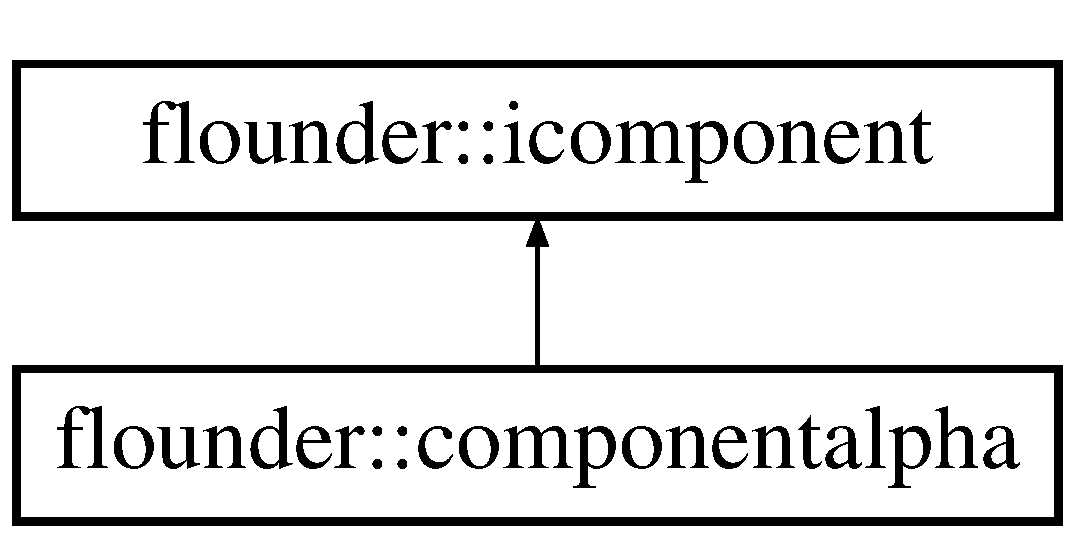
\includegraphics[height=2.000000cm]{classflounder_1_1componentalpha}
\end{center}
\end{figure}
\subsection*{Public Member Functions}
\begin{DoxyCompactItemize}
\item 
\mbox{\Hypertarget{classflounder_1_1componentalpha_a2a17cd18805b75412cba03d8a7548008}\label{classflounder_1_1componentalpha_a2a17cd18805b75412cba03d8a7548008}} 
{\bfseries componentalpha} (const float \&alpha)
\item 
\mbox{\Hypertarget{classflounder_1_1componentalpha_ac4ee13545e7414cef26136377dcbbe90}\label{classflounder_1_1componentalpha_ac4ee13545e7414cef26136377dcbbe90}} 
void {\bfseries update} () override
\item 
\mbox{\Hypertarget{classflounder_1_1componentalpha_a7aff2ddc63d0851e0c581e0d8de4d42d}\label{classflounder_1_1componentalpha_a7aff2ddc63d0851e0c581e0d8de4d42d}} 
void {\bfseries render} (\hyperlink{structflounder_1_1entityrender}{entityrender} $\ast$render) override
\item 
\mbox{\Hypertarget{classflounder_1_1componentalpha_a53215e826d4e23d232735e2006d0477d}\label{classflounder_1_1componentalpha_a53215e826d4e23d232735e2006d0477d}} 
float {\bfseries get\+Alpha} () const
\item 
\mbox{\Hypertarget{classflounder_1_1componentalpha_ae2a29f176b993b5e8dc0ef973ac96bbb}\label{classflounder_1_1componentalpha_ae2a29f176b993b5e8dc0ef973ac96bbb}} 
void {\bfseries set\+Alpha} (const float \&alpha)
\end{DoxyCompactItemize}
\subsection*{Private Attributes}
\begin{DoxyCompactItemize}
\item 
\mbox{\Hypertarget{classflounder_1_1componentalpha_a8d2368973e8284337e85af6f01c13e06}\label{classflounder_1_1componentalpha_a8d2368973e8284337e85af6f01c13e06}} 
float {\bfseries m\+\_\+alpha}
\end{DoxyCompactItemize}
\subsection*{Additional Inherited Members}


The documentation for this class was generated from the following files\+:\begin{DoxyCompactItemize}
\item 
Flounder-\/\+Core/src/entities/components/componentalpha.\+h\item 
Flounder-\/\+Core/src/entities/components/componentalpha.\+cpp\end{DoxyCompactItemize}

\hypertarget{classflounder_1_1containerscreen}{}\section{flounder\+:\+:containerscreen Class Reference}
\label{classflounder_1_1containerscreen}\index{flounder\+::containerscreen@{flounder\+::containerscreen}}


A gui object that has a empty update and delete method.  




{\ttfamily \#include $<$containerscreen.\+h$>$}

Inheritance diagram for flounder\+:\+:containerscreen\+:\begin{figure}[H]
\begin{center}
\leavevmode
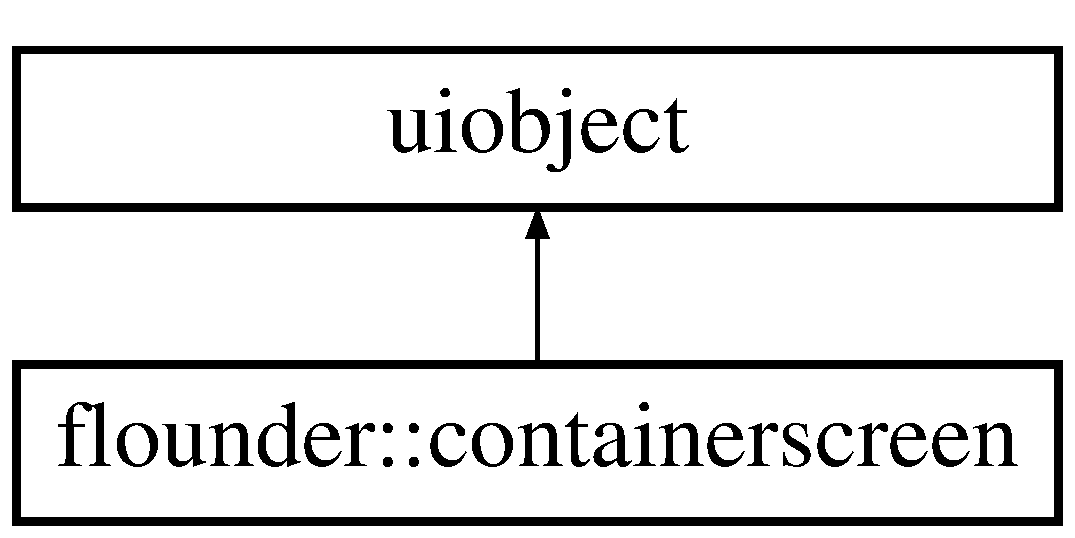
\includegraphics[height=2.000000cm]{classflounder_1_1containerscreen}
\end{center}
\end{figure}
\subsection*{Public Member Functions}
\begin{DoxyCompactItemize}
\item 
\mbox{\Hypertarget{classflounder_1_1containerscreen_a7ba6b3975a5edce6febffcd1650ac86b}\label{classflounder_1_1containerscreen_a7ba6b3975a5edce6febffcd1650ac86b}} 
{\bfseries containerscreen} (uiobject $\ast$parent, const \hyperlink{classflounder_1_1vector2}{vector2} \&position, const \hyperlink{classflounder_1_1vector2}{vector2} \&dimensions, const bool \&in\+Screen\+Coords)
\item 
\mbox{\Hypertarget{classflounder_1_1containerscreen_a6ad94c2ef6a63b172dfc1d07596c6bad}\label{classflounder_1_1containerscreen_a6ad94c2ef6a63b172dfc1d07596c6bad}} 
void {\bfseries update\+Object} () override
\end{DoxyCompactItemize}


\subsection{Detailed Description}
A gui object that has a empty update and delete method. 



The documentation for this class was generated from the following files\+:\begin{DoxyCompactItemize}
\item 
Flounder-\/\+Core/src/uis/containerscreen.\+h\item 
Flounder-\/\+Core/src/uis/containerscreen.\+cpp\end{DoxyCompactItemize}

\hypertarget{classflounder_1_1delta}{}\section{flounder\+:\+:delta Class Reference}
\label{classflounder_1_1delta}\index{flounder\+::delta@{flounder\+::delta}}


A class for handing and calculating deltas.  




{\ttfamily \#include $<$delta.\+h$>$}

\subsection*{Public Member Functions}
\begin{DoxyCompactItemize}
\item 
\hyperlink{classflounder_1_1delta_a6996799d2f9423e994e2beb84dc3ba09}{delta} ()
\begin{DoxyCompactList}\small\item\em Creates a new change handler. \end{DoxyCompactList}\item 
\hyperlink{classflounder_1_1delta_af9eb174b15b3730a45a903e988dac1e8}{$\sim$delta} ()
\begin{DoxyCompactList}\small\item\em Deconstructor for the delta. \end{DoxyCompactList}\item 
void \hyperlink{classflounder_1_1delta_a6f87fd0b76d229ec490a07a565c2afd0}{update} ()
\begin{DoxyCompactList}\small\item\em Updates change and times. \end{DoxyCompactList}\item 
\mbox{\Hypertarget{classflounder_1_1delta_ac1807f994e592b1f04447dbddcdacb9f}\label{classflounder_1_1delta_ac1807f994e592b1f04447dbddcdacb9f}} 
float {\bfseries get\+Change} () const
\item 
\mbox{\Hypertarget{classflounder_1_1delta_a9db78508227a6e75540985cb1d538ec1}\label{classflounder_1_1delta_a9db78508227a6e75540985cb1d538ec1}} 
float {\bfseries get\+Time} () const
\end{DoxyCompactItemize}
\subsection*{Private Attributes}
\begin{DoxyCompactItemize}
\item 
\mbox{\Hypertarget{classflounder_1_1delta_acb0bc7ee712e050a8b9d5974bc5d5e2a}\label{classflounder_1_1delta_acb0bc7ee712e050a8b9d5974bc5d5e2a}} 
float {\bfseries m\+\_\+current\+Frame\+Time}
\item 
\mbox{\Hypertarget{classflounder_1_1delta_a36a3f21ac4ec4c3c2216fc8df280e708}\label{classflounder_1_1delta_a36a3f21ac4ec4c3c2216fc8df280e708}} 
float {\bfseries m\+\_\+last\+Frame\+Time}
\item 
\mbox{\Hypertarget{classflounder_1_1delta_a3dea092447bed123f16b7f8a3545e828}\label{classflounder_1_1delta_a3dea092447bed123f16b7f8a3545e828}} 
float {\bfseries m\+\_\+change}
\item 
\mbox{\Hypertarget{classflounder_1_1delta_aeb8c04e49b5dd6244bd3fe97736cb468}\label{classflounder_1_1delta_aeb8c04e49b5dd6244bd3fe97736cb468}} 
float {\bfseries m\+\_\+time}
\end{DoxyCompactItemize}


\subsection{Detailed Description}
A class for handing and calculating deltas. 



\subsection{Constructor \& Destructor Documentation}
\mbox{\Hypertarget{classflounder_1_1delta_a6996799d2f9423e994e2beb84dc3ba09}\label{classflounder_1_1delta_a6996799d2f9423e994e2beb84dc3ba09}} 
\index{flounder\+::delta@{flounder\+::delta}!delta@{delta}}
\index{delta@{delta}!flounder\+::delta@{flounder\+::delta}}
\subsubsection{\texorpdfstring{delta()}{delta()}}
{\footnotesize\ttfamily flounder\+::delta\+::delta (\begin{DoxyParamCaption}{ }\end{DoxyParamCaption})}



Creates a new change handler. 

\mbox{\Hypertarget{classflounder_1_1delta_af9eb174b15b3730a45a903e988dac1e8}\label{classflounder_1_1delta_af9eb174b15b3730a45a903e988dac1e8}} 
\index{flounder\+::delta@{flounder\+::delta}!````~delta@{$\sim$delta}}
\index{````~delta@{$\sim$delta}!flounder\+::delta@{flounder\+::delta}}
\subsubsection{\texorpdfstring{$\sim$delta()}{~delta()}}
{\footnotesize\ttfamily flounder\+::delta\+::$\sim$delta (\begin{DoxyParamCaption}{ }\end{DoxyParamCaption})}



Deconstructor for the delta. 



\subsection{Member Function Documentation}
\mbox{\Hypertarget{classflounder_1_1delta_a6f87fd0b76d229ec490a07a565c2afd0}\label{classflounder_1_1delta_a6f87fd0b76d229ec490a07a565c2afd0}} 
\index{flounder\+::delta@{flounder\+::delta}!update@{update}}
\index{update@{update}!flounder\+::delta@{flounder\+::delta}}
\subsubsection{\texorpdfstring{update()}{update()}}
{\footnotesize\ttfamily void flounder\+::delta\+::update (\begin{DoxyParamCaption}{ }\end{DoxyParamCaption})}



Updates change and times. 



The documentation for this class was generated from the following files\+:\begin{DoxyCompactItemize}
\item 
Flounder-\/\+Core/src/maths/delta.\+h\item 
Flounder-\/\+Core/src/maths/delta.\+cpp\end{DoxyCompactItemize}

\hypertarget{classflounder_1_1display}{}\section{flounder\+:\+:display Class Reference}
\label{classflounder_1_1display}\index{flounder\+::display@{flounder\+::display}}


A module used for the creation, updating and destruction of the display.  




{\ttfamily \#include $<$display.\+h$>$}

Inheritance diagram for flounder\+:\+:display\+:\begin{figure}[H]
\begin{center}
\leavevmode
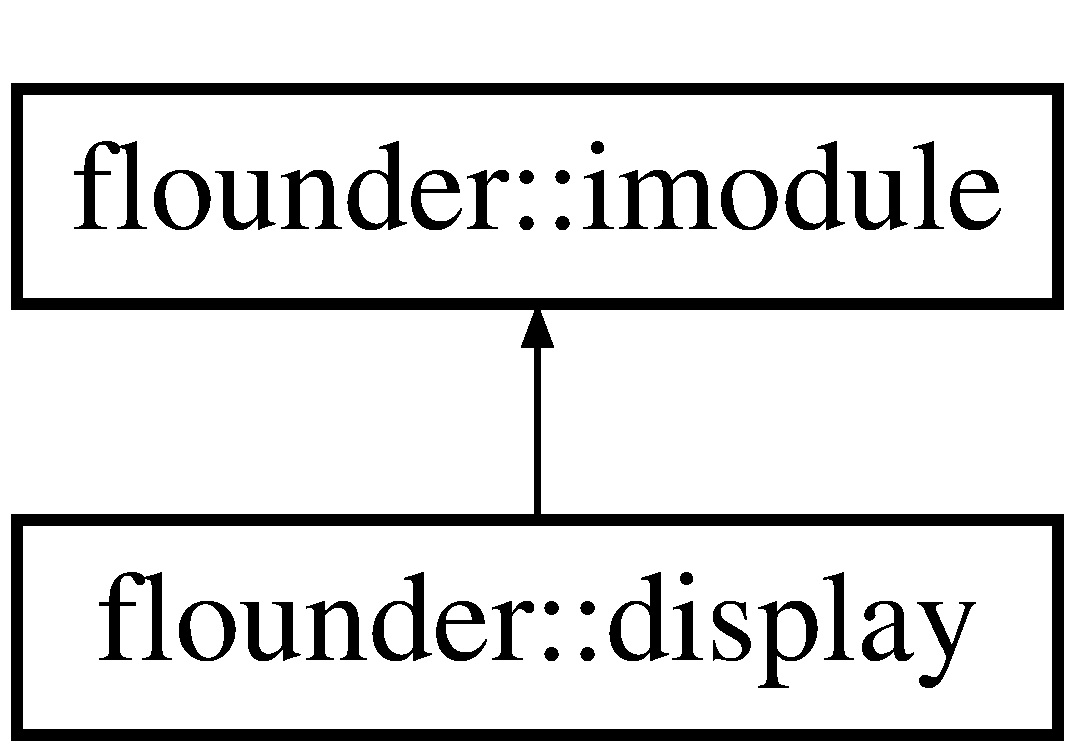
\includegraphics[height=2.000000cm]{classflounder_1_1display}
\end{center}
\end{figure}
\subsection*{Public Member Functions}
\begin{DoxyCompactItemize}
\item 
\hyperlink{classflounder_1_1display_ac0a3910222a928f1fc60193cd65c0530}{display} ()
\begin{DoxyCompactList}\small\item\em Creates a new display module. \end{DoxyCompactList}\item 
\hyperlink{classflounder_1_1display_a272f9080af9079cbb3890b18c3e4d394}{$\sim$display} ()
\begin{DoxyCompactList}\small\item\em Deconstructor for the display module. \end{DoxyCompactList}\item 
void \hyperlink{classflounder_1_1display_a799c6a76fcac1a0ca56dfd6b8d7993fa}{update} () override
\begin{DoxyCompactList}\small\item\em The update function for the module. \end{DoxyCompactList}\item 
void \hyperlink{classflounder_1_1display_af27b3f93977c32c79ad9522672e484c5}{screenshot} ()
\begin{DoxyCompactList}\small\item\em Takes a screenshot of the current image of the display and saves it into the screenshots folder a png image. \end{DoxyCompactList}\item 
int \hyperlink{classflounder_1_1display_a5e6a9e9ea60e2f8d0850ea689abb0569}{get\+Glfw\+Major} ()
\begin{DoxyCompactList}\small\item\em Gets the G\+L\+FW major verson. \end{DoxyCompactList}\item 
int \hyperlink{classflounder_1_1display_ac6fbd123308dce6a0d8f281a9ea55b37}{get\+Glfw\+Minor} ()
\begin{DoxyCompactList}\small\item\em Gets the G\+L\+FW minor verson. \end{DoxyCompactList}\item 
int \& \hyperlink{classflounder_1_1display_ac2b45bb8c8924b985895f2b08c03c3d9}{get\+Width} ()
\begin{DoxyCompactList}\small\item\em Gets the width of the display in pixels. \end{DoxyCompactList}\item 
int \& \hyperlink{classflounder_1_1display_ac47027c6b34d260ccaf148e4e762cdbe}{get\+Window\+Width} ()
\begin{DoxyCompactList}\small\item\em Gets the non-\/fullscreen width of the display in pixels. \end{DoxyCompactList}\item 
int \& \hyperlink{classflounder_1_1display_a2b3cea6e41121de9d790acf027036167}{get\+Height} ()
\begin{DoxyCompactList}\small\item\em Gets the height of the display in pixels. \end{DoxyCompactList}\item 
int \& \hyperlink{classflounder_1_1display_af1d306cb8353a7cdfe7daae4727028fc}{get\+Window\+Height} ()
\begin{DoxyCompactList}\small\item\em Gets the non-\/fullscreen height of the display in pixels. \end{DoxyCompactList}\item 
double \& \hyperlink{classflounder_1_1display_a7b32aeb7809ad48663ce6eb4596b37a3}{get\+Aspect\+Ratio} ()
\begin{DoxyCompactList}\small\item\em Gets the aspect ratio between the displays width and height. \end{DoxyCompactList}\item 
void \hyperlink{classflounder_1_1display_a13edcfe35505b3e164010ed1b232e5d1}{set\+Window\+Size} (const int \&width, const int \&height)
\begin{DoxyCompactList}\small\item\em Sets window size to a new size. \end{DoxyCompactList}\item 
std\+::string \& \hyperlink{classflounder_1_1display_ad5fc46c79d236783ac883878ec065f36}{get\+Title} ()
\begin{DoxyCompactList}\small\item\em Gets the window\textquotesingle{}s title. \end{DoxyCompactList}\item 
void \hyperlink{classflounder_1_1display_a48680d3ed1b6842dea7eb5437d6c336f}{set\+Title} (const std\+::string \&title)
\begin{DoxyCompactList}\small\item\em Sets window title \end{DoxyCompactList}\item 
std\+::string \& \hyperlink{classflounder_1_1display_ac0506da092e74addb30ca2ecb9b5a0d5}{get\+Icon} ()
\begin{DoxyCompactList}\small\item\em Gets the window\textquotesingle{}s icon file. \end{DoxyCompactList}\item 
void \hyperlink{classflounder_1_1display_a49ba8d850f666496fabf9133d01091ab}{set\+Icon} (const std\+::string \&icon)
\begin{DoxyCompactList}\small\item\em Sets window icon image. \end{DoxyCompactList}\item 
int \hyperlink{classflounder_1_1display_aea9d5368ecd65c53e634d1cec52f9718}{get\+Fps\+Limit} ()
\begin{DoxyCompactList}\small\item\em Gets the fps limit. \end{DoxyCompactList}\item 
void \hyperlink{classflounder_1_1display_a7d24403c951e5a043675c3e7b02c3c34}{set\+Fps\+Limit} (const int \&fps\+Limit)
\begin{DoxyCompactList}\small\item\em Sets the fps limit. -\/1 disables limits. \end{DoxyCompactList}\item 
bool \hyperlink{classflounder_1_1display_a75f2ff773d4d26740df8531b20b0a091}{is\+V\+Sync} ()
\begin{DoxyCompactList}\small\item\em Gets if the display is using v\+Sync. \end{DoxyCompactList}\item 
void \hyperlink{classflounder_1_1display_a172501e1e99cde228d86fab59a3a636b}{set\+V\+Sync} (const bool \&vsync)
\begin{DoxyCompactList}\small\item\em Sets the display to use V\+Sync or not. \end{DoxyCompactList}\item 
bool \hyperlink{classflounder_1_1display_ab36d40e6a3be5272853e13e45da750b8}{is\+Antialiasing} ()
\begin{DoxyCompactList}\small\item\em Gets if the display requests antialiased images. \end{DoxyCompactList}\item 
void \hyperlink{classflounder_1_1display_ae9a340bfa09dfd6d08ebc0d21b4c77b0}{set\+Antialiasing} (const bool \&antialiasing)
\begin{DoxyCompactList}\small\item\em Requests the display to antialias. \end{DoxyCompactList}\item 
int \hyperlink{classflounder_1_1display_a3f1438e0d64121ae94e3e1f1931dc09a}{get\+Samples} ()
\begin{DoxyCompactList}\small\item\em Gets how many M\+S\+AA samples should be done before swapping buffers. \end{DoxyCompactList}\item 
void \hyperlink{classflounder_1_1display_ae1bf2028faaf411fedc80ca511a2e739}{set\+Samples} (const int \&samples)
\begin{DoxyCompactList}\small\item\em Gets how many M\+S\+AA samples should be done before swapping buffers. Zero disables multisampling. G\+L\+F\+W\+\_\+\+D\+O\+N\+T\+\_\+\+C\+A\+RE means no preference. \end{DoxyCompactList}\item 
bool \hyperlink{classflounder_1_1display_ad9a50aad9e26ea3f3a074d1dbe19c58a}{is\+Fullscreen} ()
\begin{DoxyCompactList}\small\item\em Gets weather the display is fullscreen or not. \end{DoxyCompactList}\item 
void \hyperlink{classflounder_1_1display_ae5ee27f982e6a947305dc6e71a23021b}{set\+Fullscreen} (const bool \&fullscreen)
\begin{DoxyCompactList}\small\item\em Sets the display to be fullscreen or windowed. \end{DoxyCompactList}\item 
G\+L\+F\+Wwindow $\ast$ \hyperlink{classflounder_1_1display_a5cdcd3dddce4cf63ac45503b03e96689}{get\+Window} ()
\begin{DoxyCompactList}\small\item\em Gets the current G\+L\+FW window. \end{DoxyCompactList}\item 
bool \hyperlink{classflounder_1_1display_af187a33ad8b4e112a638adfdd3062fb3}{is\+Closed} ()
\begin{DoxyCompactList}\small\item\em Gets if the G\+L\+FW display is closed. \end{DoxyCompactList}\item 
bool \hyperlink{classflounder_1_1display_a57dbf90706399fb0511b50740a1b77da}{is\+Focused} ()
\begin{DoxyCompactList}\small\item\em Gets if the G\+L\+FW display is selected. \end{DoxyCompactList}\item 
int \hyperlink{classflounder_1_1display_adbf55bdf135324664810751f3ab27d82}{get\+Window\+X\+Pos} ()
\begin{DoxyCompactList}\small\item\em Gets the windows Y position of the display in pixels. \end{DoxyCompactList}\item 
int \hyperlink{classflounder_1_1display_a92e7674dcd56f1e3f8b617a9b3fb625d}{get\+Window\+Y\+Pos} ()
\begin{DoxyCompactList}\small\item\em Gets the windows Y position of the display in pixels. \end{DoxyCompactList}\end{DoxyCompactItemize}
\subsection*{Static Public Member Functions}
\begin{DoxyCompactItemize}
\item 
static \hyperlink{classflounder_1_1display}{display} $\ast$ \hyperlink{classflounder_1_1display_a7c7015939f48bf4526bb0330ea4fcd2f}{get} ()
\begin{DoxyCompactList}\small\item\em Gets this framework instance. \end{DoxyCompactList}\end{DoxyCompactItemize}
\subsection*{Private Attributes}
\begin{DoxyCompactItemize}
\item 
\mbox{\Hypertarget{classflounder_1_1display_ac6adba7cfd74600fbb124758d81f3fef}\label{classflounder_1_1display_ac6adba7cfd74600fbb124758d81f3fef}} 
int {\bfseries m\+\_\+glfw\+Major}
\item 
\mbox{\Hypertarget{classflounder_1_1display_abe5ded7b2a974c3be4f45a67460cbff1}\label{classflounder_1_1display_abe5ded7b2a974c3be4f45a67460cbff1}} 
int {\bfseries m\+\_\+glfw\+Minor}
\item 
\mbox{\Hypertarget{classflounder_1_1display_a860cf35cfa01a455432e56da56b42715}\label{classflounder_1_1display_a860cf35cfa01a455432e56da56b42715}} 
int {\bfseries m\+\_\+window\+Width}
\item 
\mbox{\Hypertarget{classflounder_1_1display_ac645ec5d7726988bc1bf9d1ea3bc92d1}\label{classflounder_1_1display_ac645ec5d7726988bc1bf9d1ea3bc92d1}} 
int {\bfseries m\+\_\+window\+Height}
\item 
\mbox{\Hypertarget{classflounder_1_1display_ad4970ad3855b5b34565f6c5fe17ee383}\label{classflounder_1_1display_ad4970ad3855b5b34565f6c5fe17ee383}} 
int {\bfseries m\+\_\+fullscreen\+Width}
\item 
\mbox{\Hypertarget{classflounder_1_1display_a5ba749a0a474ac113ec21fbbb0544688}\label{classflounder_1_1display_a5ba749a0a474ac113ec21fbbb0544688}} 
int {\bfseries m\+\_\+fullscreen\+Height}
\item 
\mbox{\Hypertarget{classflounder_1_1display_a54d05378c6c5085ed6c49ff94fa8c4b0}\label{classflounder_1_1display_a54d05378c6c5085ed6c49ff94fa8c4b0}} 
double {\bfseries m\+\_\+aspect\+Ratio}
\item 
\mbox{\Hypertarget{classflounder_1_1display_a2c2b649d019390dab458de301bb57c01}\label{classflounder_1_1display_a2c2b649d019390dab458de301bb57c01}} 
std\+::string {\bfseries m\+\_\+title}
\item 
\mbox{\Hypertarget{classflounder_1_1display_a4d7ba13c8c98370491cd396e4530dc8d}\label{classflounder_1_1display_a4d7ba13c8c98370491cd396e4530dc8d}} 
std\+::string {\bfseries m\+\_\+icon}
\item 
\mbox{\Hypertarget{classflounder_1_1display_a1409aa430c7fd27729d69ba8d992e9ac}\label{classflounder_1_1display_a1409aa430c7fd27729d69ba8d992e9ac}} 
float {\bfseries m\+\_\+fps\+Limit}
\item 
\mbox{\Hypertarget{classflounder_1_1display_a43e081e66465e2cc75a5cca35d81a81f}\label{classflounder_1_1display_a43e081e66465e2cc75a5cca35d81a81f}} 
bool {\bfseries m\+\_\+vsync}
\item 
\mbox{\Hypertarget{classflounder_1_1display_af6818746f20ea2cbb50e9fcdae3ffa75}\label{classflounder_1_1display_af6818746f20ea2cbb50e9fcdae3ffa75}} 
bool {\bfseries m\+\_\+antialiasing}
\item 
\mbox{\Hypertarget{classflounder_1_1display_ace88ce0f05106aefbd44cc2a45b6c448}\label{classflounder_1_1display_ace88ce0f05106aefbd44cc2a45b6c448}} 
int {\bfseries m\+\_\+samples}
\item 
\mbox{\Hypertarget{classflounder_1_1display_a738b31e17f1cfaba3832829dd9ee4bc0}\label{classflounder_1_1display_a738b31e17f1cfaba3832829dd9ee4bc0}} 
bool {\bfseries m\+\_\+fullscreen}
\item 
\mbox{\Hypertarget{classflounder_1_1display_a264c3a43ec52675d327e2912743d70da}\label{classflounder_1_1display_a264c3a43ec52675d327e2912743d70da}} 
G\+L\+F\+Wwindow $\ast$ {\bfseries m\+\_\+window}
\item 
\mbox{\Hypertarget{classflounder_1_1display_a8c238cb4806c6dd0610a8edff1e75471}\label{classflounder_1_1display_a8c238cb4806c6dd0610a8edff1e75471}} 
bool {\bfseries m\+\_\+closed}
\item 
\mbox{\Hypertarget{classflounder_1_1display_a4ab2cf4e642518efcc8f1b6d9d6dda84}\label{classflounder_1_1display_a4ab2cf4e642518efcc8f1b6d9d6dda84}} 
bool {\bfseries m\+\_\+focused}
\item 
\mbox{\Hypertarget{classflounder_1_1display_a31c63bef47c639477a34f71fe086cea5}\label{classflounder_1_1display_a31c63bef47c639477a34f71fe086cea5}} 
int {\bfseries m\+\_\+window\+PosX}
\item 
\mbox{\Hypertarget{classflounder_1_1display_a63d9f9bd2d295379fc53a8c2b9efba78}\label{classflounder_1_1display_a63d9f9bd2d295379fc53a8c2b9efba78}} 
int {\bfseries m\+\_\+window\+PosY}
\end{DoxyCompactItemize}
\subsection*{Friends}
\begin{DoxyCompactItemize}
\item 
\mbox{\Hypertarget{classflounder_1_1display_a6e2f7636c5e3fe93e7ae254f055d2ac1}\label{classflounder_1_1display_a6e2f7636c5e3fe93e7ae254f055d2ac1}} 
void {\bfseries callback\+Error} (int error, const char $\ast$description)
\item 
\mbox{\Hypertarget{classflounder_1_1display_ad1fb7c8678d6c41a7b539440f01df61e}\label{classflounder_1_1display_ad1fb7c8678d6c41a7b539440f01df61e}} 
void {\bfseries callback\+Close} (G\+L\+F\+Wwindow $\ast$window)
\item 
\mbox{\Hypertarget{classflounder_1_1display_ac00c6be12bf18837bd3960c3ba402f3f}\label{classflounder_1_1display_ac00c6be12bf18837bd3960c3ba402f3f}} 
void {\bfseries callback\+Focus} (G\+L\+F\+Wwindow $\ast$window, int focused)
\item 
\mbox{\Hypertarget{classflounder_1_1display_a39d3d8fb74851349d8a437aa6a3f2b35}\label{classflounder_1_1display_a39d3d8fb74851349d8a437aa6a3f2b35}} 
void {\bfseries callback\+Position} (G\+L\+F\+Wwindow $\ast$window, int xpos, int ypos)
\item 
\mbox{\Hypertarget{classflounder_1_1display_af765170864757051f6a767c26700bb82}\label{classflounder_1_1display_af765170864757051f6a767c26700bb82}} 
void {\bfseries callback\+Size} (G\+L\+F\+Wwindow $\ast$window, int width, int height)
\item 
\mbox{\Hypertarget{classflounder_1_1display_a0d3e5fdd07e5059768ff51de12b0b29f}\label{classflounder_1_1display_a0d3e5fdd07e5059768ff51de12b0b29f}} 
void {\bfseries callback\+Frame} (G\+L\+F\+Wwindow $\ast$window, int width, int height)
\end{DoxyCompactItemize}


\subsection{Detailed Description}
A module used for the creation, updating and destruction of the display. 



\subsection{Constructor \& Destructor Documentation}
\mbox{\Hypertarget{classflounder_1_1display_ac0a3910222a928f1fc60193cd65c0530}\label{classflounder_1_1display_ac0a3910222a928f1fc60193cd65c0530}} 
\index{flounder\+::display@{flounder\+::display}!display@{display}}
\index{display@{display}!flounder\+::display@{flounder\+::display}}
\subsubsection{\texorpdfstring{display()}{display()}}
{\footnotesize\ttfamily flounder\+::display\+::display (\begin{DoxyParamCaption}{ }\end{DoxyParamCaption})}



Creates a new display module. 

\mbox{\Hypertarget{classflounder_1_1display_a272f9080af9079cbb3890b18c3e4d394}\label{classflounder_1_1display_a272f9080af9079cbb3890b18c3e4d394}} 
\index{flounder\+::display@{flounder\+::display}!````~display@{$\sim$display}}
\index{````~display@{$\sim$display}!flounder\+::display@{flounder\+::display}}
\subsubsection{\texorpdfstring{$\sim$display()}{~display()}}
{\footnotesize\ttfamily flounder\+::display\+::$\sim$display (\begin{DoxyParamCaption}{ }\end{DoxyParamCaption})}



Deconstructor for the display module. 



\subsection{Member Function Documentation}
\mbox{\Hypertarget{classflounder_1_1display_a7c7015939f48bf4526bb0330ea4fcd2f}\label{classflounder_1_1display_a7c7015939f48bf4526bb0330ea4fcd2f}} 
\index{flounder\+::display@{flounder\+::display}!get@{get}}
\index{get@{get}!flounder\+::display@{flounder\+::display}}
\subsubsection{\texorpdfstring{get()}{get()}}
{\footnotesize\ttfamily static \hyperlink{classflounder_1_1display}{display}$\ast$ flounder\+::display\+::get (\begin{DoxyParamCaption}{ }\end{DoxyParamCaption})\hspace{0.3cm}{\ttfamily [inline]}, {\ttfamily [static]}}



Gets this framework instance. 

\begin{DoxyReturn}{Returns}
The current module instance. 
\end{DoxyReturn}
\mbox{\Hypertarget{classflounder_1_1display_a7b32aeb7809ad48663ce6eb4596b37a3}\label{classflounder_1_1display_a7b32aeb7809ad48663ce6eb4596b37a3}} 
\index{flounder\+::display@{flounder\+::display}!get\+Aspect\+Ratio@{get\+Aspect\+Ratio}}
\index{get\+Aspect\+Ratio@{get\+Aspect\+Ratio}!flounder\+::display@{flounder\+::display}}
\subsubsection{\texorpdfstring{get\+Aspect\+Ratio()}{getAspectRatio()}}
{\footnotesize\ttfamily double \& flounder\+::display\+::get\+Aspect\+Ratio (\begin{DoxyParamCaption}{ }\end{DoxyParamCaption})}



Gets the aspect ratio between the displays width and height. 

\begin{DoxyReturn}{Returns}
The aspect ratio. 
\end{DoxyReturn}
\mbox{\Hypertarget{classflounder_1_1display_aea9d5368ecd65c53e634d1cec52f9718}\label{classflounder_1_1display_aea9d5368ecd65c53e634d1cec52f9718}} 
\index{flounder\+::display@{flounder\+::display}!get\+Fps\+Limit@{get\+Fps\+Limit}}
\index{get\+Fps\+Limit@{get\+Fps\+Limit}!flounder\+::display@{flounder\+::display}}
\subsubsection{\texorpdfstring{get\+Fps\+Limit()}{getFpsLimit()}}
{\footnotesize\ttfamily int flounder\+::display\+::get\+Fps\+Limit (\begin{DoxyParamCaption}{ }\end{DoxyParamCaption})}



Gets the fps limit. 

\begin{DoxyReturn}{Returns}
The fps limit. 
\end{DoxyReturn}
\mbox{\Hypertarget{classflounder_1_1display_a5e6a9e9ea60e2f8d0850ea689abb0569}\label{classflounder_1_1display_a5e6a9e9ea60e2f8d0850ea689abb0569}} 
\index{flounder\+::display@{flounder\+::display}!get\+Glfw\+Major@{get\+Glfw\+Major}}
\index{get\+Glfw\+Major@{get\+Glfw\+Major}!flounder\+::display@{flounder\+::display}}
\subsubsection{\texorpdfstring{get\+Glfw\+Major()}{getGlfwMajor()}}
{\footnotesize\ttfamily int flounder\+::display\+::get\+Glfw\+Major (\begin{DoxyParamCaption}{ }\end{DoxyParamCaption})\hspace{0.3cm}{\ttfamily [inline]}}



Gets the G\+L\+FW major verson. 

\begin{DoxyReturn}{Returns}
The G\+L\+FW major verson. 
\end{DoxyReturn}
\mbox{\Hypertarget{classflounder_1_1display_ac6fbd123308dce6a0d8f281a9ea55b37}\label{classflounder_1_1display_ac6fbd123308dce6a0d8f281a9ea55b37}} 
\index{flounder\+::display@{flounder\+::display}!get\+Glfw\+Minor@{get\+Glfw\+Minor}}
\index{get\+Glfw\+Minor@{get\+Glfw\+Minor}!flounder\+::display@{flounder\+::display}}
\subsubsection{\texorpdfstring{get\+Glfw\+Minor()}{getGlfwMinor()}}
{\footnotesize\ttfamily int flounder\+::display\+::get\+Glfw\+Minor (\begin{DoxyParamCaption}{ }\end{DoxyParamCaption})\hspace{0.3cm}{\ttfamily [inline]}}



Gets the G\+L\+FW minor verson. 

\begin{DoxyReturn}{Returns}
The G\+L\+FW minor verson. 
\end{DoxyReturn}
\mbox{\Hypertarget{classflounder_1_1display_a2b3cea6e41121de9d790acf027036167}\label{classflounder_1_1display_a2b3cea6e41121de9d790acf027036167}} 
\index{flounder\+::display@{flounder\+::display}!get\+Height@{get\+Height}}
\index{get\+Height@{get\+Height}!flounder\+::display@{flounder\+::display}}
\subsubsection{\texorpdfstring{get\+Height()}{getHeight()}}
{\footnotesize\ttfamily int \& flounder\+::display\+::get\+Height (\begin{DoxyParamCaption}{ }\end{DoxyParamCaption})}



Gets the height of the display in pixels. 

\begin{DoxyReturn}{Returns}
The height of the display. 
\end{DoxyReturn}
\mbox{\Hypertarget{classflounder_1_1display_ac0506da092e74addb30ca2ecb9b5a0d5}\label{classflounder_1_1display_ac0506da092e74addb30ca2ecb9b5a0d5}} 
\index{flounder\+::display@{flounder\+::display}!get\+Icon@{get\+Icon}}
\index{get\+Icon@{get\+Icon}!flounder\+::display@{flounder\+::display}}
\subsubsection{\texorpdfstring{get\+Icon()}{getIcon()}}
{\footnotesize\ttfamily std\+::string \& flounder\+::display\+::get\+Icon (\begin{DoxyParamCaption}{ }\end{DoxyParamCaption})}



Gets the window\textquotesingle{}s icon file. 

\begin{DoxyReturn}{Returns}
The window\textquotesingle{}s icon file. 
\end{DoxyReturn}
\mbox{\Hypertarget{classflounder_1_1display_a3f1438e0d64121ae94e3e1f1931dc09a}\label{classflounder_1_1display_a3f1438e0d64121ae94e3e1f1931dc09a}} 
\index{flounder\+::display@{flounder\+::display}!get\+Samples@{get\+Samples}}
\index{get\+Samples@{get\+Samples}!flounder\+::display@{flounder\+::display}}
\subsubsection{\texorpdfstring{get\+Samples()}{getSamples()}}
{\footnotesize\ttfamily int flounder\+::display\+::get\+Samples (\begin{DoxyParamCaption}{ }\end{DoxyParamCaption})}



Gets how many M\+S\+AA samples should be done before swapping buffers. 

\begin{DoxyReturn}{Returns}
Amount of M\+S\+AA samples. 
\end{DoxyReturn}
\mbox{\Hypertarget{classflounder_1_1display_ad5fc46c79d236783ac883878ec065f36}\label{classflounder_1_1display_ad5fc46c79d236783ac883878ec065f36}} 
\index{flounder\+::display@{flounder\+::display}!get\+Title@{get\+Title}}
\index{get\+Title@{get\+Title}!flounder\+::display@{flounder\+::display}}
\subsubsection{\texorpdfstring{get\+Title()}{getTitle()}}
{\footnotesize\ttfamily std\+::string \& flounder\+::display\+::get\+Title (\begin{DoxyParamCaption}{ }\end{DoxyParamCaption})}



Gets the window\textquotesingle{}s title. 

\begin{DoxyReturn}{Returns}
The window\textquotesingle{}s title. 
\end{DoxyReturn}
\mbox{\Hypertarget{classflounder_1_1display_ac2b45bb8c8924b985895f2b08c03c3d9}\label{classflounder_1_1display_ac2b45bb8c8924b985895f2b08c03c3d9}} 
\index{flounder\+::display@{flounder\+::display}!get\+Width@{get\+Width}}
\index{get\+Width@{get\+Width}!flounder\+::display@{flounder\+::display}}
\subsubsection{\texorpdfstring{get\+Width()}{getWidth()}}
{\footnotesize\ttfamily int \& flounder\+::display\+::get\+Width (\begin{DoxyParamCaption}{ }\end{DoxyParamCaption})}



Gets the width of the display in pixels. 

\begin{DoxyReturn}{Returns}
The width of the display. 
\end{DoxyReturn}
\mbox{\Hypertarget{classflounder_1_1display_a5cdcd3dddce4cf63ac45503b03e96689}\label{classflounder_1_1display_a5cdcd3dddce4cf63ac45503b03e96689}} 
\index{flounder\+::display@{flounder\+::display}!get\+Window@{get\+Window}}
\index{get\+Window@{get\+Window}!flounder\+::display@{flounder\+::display}}
\subsubsection{\texorpdfstring{get\+Window()}{getWindow()}}
{\footnotesize\ttfamily G\+L\+F\+Wwindow $\ast$ flounder\+::display\+::get\+Window (\begin{DoxyParamCaption}{ }\end{DoxyParamCaption})}



Gets the current G\+L\+FW window. 

\begin{DoxyReturn}{Returns}
The current G\+L\+FW window. 
\end{DoxyReturn}
\mbox{\Hypertarget{classflounder_1_1display_af1d306cb8353a7cdfe7daae4727028fc}\label{classflounder_1_1display_af1d306cb8353a7cdfe7daae4727028fc}} 
\index{flounder\+::display@{flounder\+::display}!get\+Window\+Height@{get\+Window\+Height}}
\index{get\+Window\+Height@{get\+Window\+Height}!flounder\+::display@{flounder\+::display}}
\subsubsection{\texorpdfstring{get\+Window\+Height()}{getWindowHeight()}}
{\footnotesize\ttfamily int \& flounder\+::display\+::get\+Window\+Height (\begin{DoxyParamCaption}{ }\end{DoxyParamCaption})}



Gets the non-\/fullscreen height of the display in pixels. 

\begin{DoxyReturn}{Returns}
The height of the display. 
\end{DoxyReturn}
\mbox{\Hypertarget{classflounder_1_1display_ac47027c6b34d260ccaf148e4e762cdbe}\label{classflounder_1_1display_ac47027c6b34d260ccaf148e4e762cdbe}} 
\index{flounder\+::display@{flounder\+::display}!get\+Window\+Width@{get\+Window\+Width}}
\index{get\+Window\+Width@{get\+Window\+Width}!flounder\+::display@{flounder\+::display}}
\subsubsection{\texorpdfstring{get\+Window\+Width()}{getWindowWidth()}}
{\footnotesize\ttfamily int \& flounder\+::display\+::get\+Window\+Width (\begin{DoxyParamCaption}{ }\end{DoxyParamCaption})}



Gets the non-\/fullscreen width of the display in pixels. 

\begin{DoxyReturn}{Returns}
The width of the display. 
\end{DoxyReturn}
\mbox{\Hypertarget{classflounder_1_1display_adbf55bdf135324664810751f3ab27d82}\label{classflounder_1_1display_adbf55bdf135324664810751f3ab27d82}} 
\index{flounder\+::display@{flounder\+::display}!get\+Window\+X\+Pos@{get\+Window\+X\+Pos}}
\index{get\+Window\+X\+Pos@{get\+Window\+X\+Pos}!flounder\+::display@{flounder\+::display}}
\subsubsection{\texorpdfstring{get\+Window\+X\+Pos()}{getWindowXPos()}}
{\footnotesize\ttfamily int flounder\+::display\+::get\+Window\+X\+Pos (\begin{DoxyParamCaption}{ }\end{DoxyParamCaption})}



Gets the windows Y position of the display in pixels. 

\begin{DoxyReturn}{Returns}
The windows x position. 
\end{DoxyReturn}
\mbox{\Hypertarget{classflounder_1_1display_a92e7674dcd56f1e3f8b617a9b3fb625d}\label{classflounder_1_1display_a92e7674dcd56f1e3f8b617a9b3fb625d}} 
\index{flounder\+::display@{flounder\+::display}!get\+Window\+Y\+Pos@{get\+Window\+Y\+Pos}}
\index{get\+Window\+Y\+Pos@{get\+Window\+Y\+Pos}!flounder\+::display@{flounder\+::display}}
\subsubsection{\texorpdfstring{get\+Window\+Y\+Pos()}{getWindowYPos()}}
{\footnotesize\ttfamily int flounder\+::display\+::get\+Window\+Y\+Pos (\begin{DoxyParamCaption}{ }\end{DoxyParamCaption})}



Gets the windows Y position of the display in pixels. 

\begin{DoxyReturn}{Returns}
The windows Y position. 
\end{DoxyReturn}
\mbox{\Hypertarget{classflounder_1_1display_ab36d40e6a3be5272853e13e45da750b8}\label{classflounder_1_1display_ab36d40e6a3be5272853e13e45da750b8}} 
\index{flounder\+::display@{flounder\+::display}!is\+Antialiasing@{is\+Antialiasing}}
\index{is\+Antialiasing@{is\+Antialiasing}!flounder\+::display@{flounder\+::display}}
\subsubsection{\texorpdfstring{is\+Antialiasing()}{isAntialiasing()}}
{\footnotesize\ttfamily bool flounder\+::display\+::is\+Antialiasing (\begin{DoxyParamCaption}{ }\end{DoxyParamCaption})}



Gets if the display requests antialiased images. 

\begin{DoxyReturn}{Returns}
If using antialiased images. 
\end{DoxyReturn}
\mbox{\Hypertarget{classflounder_1_1display_af187a33ad8b4e112a638adfdd3062fb3}\label{classflounder_1_1display_af187a33ad8b4e112a638adfdd3062fb3}} 
\index{flounder\+::display@{flounder\+::display}!is\+Closed@{is\+Closed}}
\index{is\+Closed@{is\+Closed}!flounder\+::display@{flounder\+::display}}
\subsubsection{\texorpdfstring{is\+Closed()}{isClosed()}}
{\footnotesize\ttfamily bool flounder\+::display\+::is\+Closed (\begin{DoxyParamCaption}{ }\end{DoxyParamCaption})}



Gets if the G\+L\+FW display is closed. 

\begin{DoxyReturn}{Returns}
If the G\+L\+FW display is closed. 
\end{DoxyReturn}
\mbox{\Hypertarget{classflounder_1_1display_a57dbf90706399fb0511b50740a1b77da}\label{classflounder_1_1display_a57dbf90706399fb0511b50740a1b77da}} 
\index{flounder\+::display@{flounder\+::display}!is\+Focused@{is\+Focused}}
\index{is\+Focused@{is\+Focused}!flounder\+::display@{flounder\+::display}}
\subsubsection{\texorpdfstring{is\+Focused()}{isFocused()}}
{\footnotesize\ttfamily bool flounder\+::display\+::is\+Focused (\begin{DoxyParamCaption}{ }\end{DoxyParamCaption})}



Gets if the G\+L\+FW display is selected. 

\begin{DoxyReturn}{Returns}
If the G\+L\+FW display is selected. 
\end{DoxyReturn}
\mbox{\Hypertarget{classflounder_1_1display_ad9a50aad9e26ea3f3a074d1dbe19c58a}\label{classflounder_1_1display_ad9a50aad9e26ea3f3a074d1dbe19c58a}} 
\index{flounder\+::display@{flounder\+::display}!is\+Fullscreen@{is\+Fullscreen}}
\index{is\+Fullscreen@{is\+Fullscreen}!flounder\+::display@{flounder\+::display}}
\subsubsection{\texorpdfstring{is\+Fullscreen()}{isFullscreen()}}
{\footnotesize\ttfamily bool flounder\+::display\+::is\+Fullscreen (\begin{DoxyParamCaption}{ }\end{DoxyParamCaption})}



Gets weather the display is fullscreen or not. 

\begin{DoxyReturn}{Returns}
Fullscreen or windowed. 
\end{DoxyReturn}
\mbox{\Hypertarget{classflounder_1_1display_a75f2ff773d4d26740df8531b20b0a091}\label{classflounder_1_1display_a75f2ff773d4d26740df8531b20b0a091}} 
\index{flounder\+::display@{flounder\+::display}!is\+V\+Sync@{is\+V\+Sync}}
\index{is\+V\+Sync@{is\+V\+Sync}!flounder\+::display@{flounder\+::display}}
\subsubsection{\texorpdfstring{is\+V\+Sync()}{isVSync()}}
{\footnotesize\ttfamily bool flounder\+::display\+::is\+V\+Sync (\begin{DoxyParamCaption}{ }\end{DoxyParamCaption})}



Gets if the display is using v\+Sync. 

\begin{DoxyReturn}{Returns}
If V\+Sync is enabled. 
\end{DoxyReturn}
\mbox{\Hypertarget{classflounder_1_1display_af27b3f93977c32c79ad9522672e484c5}\label{classflounder_1_1display_af27b3f93977c32c79ad9522672e484c5}} 
\index{flounder\+::display@{flounder\+::display}!screenshot@{screenshot}}
\index{screenshot@{screenshot}!flounder\+::display@{flounder\+::display}}
\subsubsection{\texorpdfstring{screenshot()}{screenshot()}}
{\footnotesize\ttfamily void flounder\+::display\+::screenshot (\begin{DoxyParamCaption}{ }\end{DoxyParamCaption})}



Takes a screenshot of the current image of the display and saves it into the screenshots folder a png image. 

\mbox{\Hypertarget{classflounder_1_1display_ae9a340bfa09dfd6d08ebc0d21b4c77b0}\label{classflounder_1_1display_ae9a340bfa09dfd6d08ebc0d21b4c77b0}} 
\index{flounder\+::display@{flounder\+::display}!set\+Antialiasing@{set\+Antialiasing}}
\index{set\+Antialiasing@{set\+Antialiasing}!flounder\+::display@{flounder\+::display}}
\subsubsection{\texorpdfstring{set\+Antialiasing()}{setAntialiasing()}}
{\footnotesize\ttfamily void flounder\+::display\+::set\+Antialiasing (\begin{DoxyParamCaption}\item[{const bool \&}]{antialiasing }\end{DoxyParamCaption})}



Requests the display to antialias. 


\begin{DoxyParams}{Parameters}
{\em antialiasing} & If the display should antialias. \\
\hline
\end{DoxyParams}
\mbox{\Hypertarget{classflounder_1_1display_a7d24403c951e5a043675c3e7b02c3c34}\label{classflounder_1_1display_a7d24403c951e5a043675c3e7b02c3c34}} 
\index{flounder\+::display@{flounder\+::display}!set\+Fps\+Limit@{set\+Fps\+Limit}}
\index{set\+Fps\+Limit@{set\+Fps\+Limit}!flounder\+::display@{flounder\+::display}}
\subsubsection{\texorpdfstring{set\+Fps\+Limit()}{setFpsLimit()}}
{\footnotesize\ttfamily void flounder\+::display\+::set\+Fps\+Limit (\begin{DoxyParamCaption}\item[{const int \&}]{fps\+Limit }\end{DoxyParamCaption})}



Sets the fps limit. -\/1 disables limits. 


\begin{DoxyParams}{Parameters}
{\em fps\+Limit} & The new fps limit. \\
\hline
\end{DoxyParams}
\mbox{\Hypertarget{classflounder_1_1display_ae5ee27f982e6a947305dc6e71a23021b}\label{classflounder_1_1display_ae5ee27f982e6a947305dc6e71a23021b}} 
\index{flounder\+::display@{flounder\+::display}!set\+Fullscreen@{set\+Fullscreen}}
\index{set\+Fullscreen@{set\+Fullscreen}!flounder\+::display@{flounder\+::display}}
\subsubsection{\texorpdfstring{set\+Fullscreen()}{setFullscreen()}}
{\footnotesize\ttfamily void flounder\+::display\+::set\+Fullscreen (\begin{DoxyParamCaption}\item[{const bool \&}]{fullscreen }\end{DoxyParamCaption})}



Sets the display to be fullscreen or windowed. 


\begin{DoxyParams}{Parameters}
{\em fullscreen} & Weather or not to be fullscreen. \\
\hline
\end{DoxyParams}
\mbox{\Hypertarget{classflounder_1_1display_a49ba8d850f666496fabf9133d01091ab}\label{classflounder_1_1display_a49ba8d850f666496fabf9133d01091ab}} 
\index{flounder\+::display@{flounder\+::display}!set\+Icon@{set\+Icon}}
\index{set\+Icon@{set\+Icon}!flounder\+::display@{flounder\+::display}}
\subsubsection{\texorpdfstring{set\+Icon()}{setIcon()}}
{\footnotesize\ttfamily void flounder\+::display\+::set\+Icon (\begin{DoxyParamCaption}\item[{const std\+::string \&}]{icon }\end{DoxyParamCaption})}



Sets window icon image. 


\begin{DoxyParams}{Parameters}
{\em title} & The new icon file. \\
\hline
\end{DoxyParams}
\mbox{\Hypertarget{classflounder_1_1display_ae1bf2028faaf411fedc80ca511a2e739}\label{classflounder_1_1display_ae1bf2028faaf411fedc80ca511a2e739}} 
\index{flounder\+::display@{flounder\+::display}!set\+Samples@{set\+Samples}}
\index{set\+Samples@{set\+Samples}!flounder\+::display@{flounder\+::display}}
\subsubsection{\texorpdfstring{set\+Samples()}{setSamples()}}
{\footnotesize\ttfamily void flounder\+::display\+::set\+Samples (\begin{DoxyParamCaption}\item[{const int \&}]{samples }\end{DoxyParamCaption})}



Gets how many M\+S\+AA samples should be done before swapping buffers. Zero disables multisampling. G\+L\+F\+W\+\_\+\+D\+O\+N\+T\+\_\+\+C\+A\+RE means no preference. 


\begin{DoxyParams}{Parameters}
{\em samples} & The amount of M\+S\+AA samples. \\
\hline
\end{DoxyParams}
\mbox{\Hypertarget{classflounder_1_1display_a48680d3ed1b6842dea7eb5437d6c336f}\label{classflounder_1_1display_a48680d3ed1b6842dea7eb5437d6c336f}} 
\index{flounder\+::display@{flounder\+::display}!set\+Title@{set\+Title}}
\index{set\+Title@{set\+Title}!flounder\+::display@{flounder\+::display}}
\subsubsection{\texorpdfstring{set\+Title()}{setTitle()}}
{\footnotesize\ttfamily void flounder\+::display\+::set\+Title (\begin{DoxyParamCaption}\item[{const std\+::string \&}]{title }\end{DoxyParamCaption})}



Sets window title 


\begin{DoxyParams}{Parameters}
{\em title} & The new title. \\
\hline
\end{DoxyParams}
\mbox{\Hypertarget{classflounder_1_1display_a172501e1e99cde228d86fab59a3a636b}\label{classflounder_1_1display_a172501e1e99cde228d86fab59a3a636b}} 
\index{flounder\+::display@{flounder\+::display}!set\+V\+Sync@{set\+V\+Sync}}
\index{set\+V\+Sync@{set\+V\+Sync}!flounder\+::display@{flounder\+::display}}
\subsubsection{\texorpdfstring{set\+V\+Sync()}{setVSync()}}
{\footnotesize\ttfamily void flounder\+::display\+::set\+V\+Sync (\begin{DoxyParamCaption}\item[{const bool \&}]{vsync }\end{DoxyParamCaption})}



Sets the display to use V\+Sync or not. 


\begin{DoxyParams}{Parameters}
{\em vsync} & Weather or not to use v\+Sync. \\
\hline
\end{DoxyParams}
\mbox{\Hypertarget{classflounder_1_1display_a13edcfe35505b3e164010ed1b232e5d1}\label{classflounder_1_1display_a13edcfe35505b3e164010ed1b232e5d1}} 
\index{flounder\+::display@{flounder\+::display}!set\+Window\+Size@{set\+Window\+Size}}
\index{set\+Window\+Size@{set\+Window\+Size}!flounder\+::display@{flounder\+::display}}
\subsubsection{\texorpdfstring{set\+Window\+Size()}{setWindowSize()}}
{\footnotesize\ttfamily void flounder\+::display\+::set\+Window\+Size (\begin{DoxyParamCaption}\item[{const int \&}]{width,  }\item[{const int \&}]{height }\end{DoxyParamCaption})}



Sets window size to a new size. 


\begin{DoxyParams}{Parameters}
{\em width} & The new width in pixels. \\
\hline
{\em height} & The new height in pixels. \\
\hline
\end{DoxyParams}
\mbox{\Hypertarget{classflounder_1_1display_a799c6a76fcac1a0ca56dfd6b8d7993fa}\label{classflounder_1_1display_a799c6a76fcac1a0ca56dfd6b8d7993fa}} 
\index{flounder\+::display@{flounder\+::display}!update@{update}}
\index{update@{update}!flounder\+::display@{flounder\+::display}}
\subsubsection{\texorpdfstring{update()}{update()}}
{\footnotesize\ttfamily void flounder\+::display\+::update (\begin{DoxyParamCaption}{ }\end{DoxyParamCaption})\hspace{0.3cm}{\ttfamily [override]}, {\ttfamily [virtual]}}



The update function for the module. 



Implements \hyperlink{classflounder_1_1imodule_a9a53d48a46b5f6b16a92b2cd8503f74a}{flounder\+::imodule}.



The documentation for this class was generated from the following files\+:\begin{DoxyCompactItemize}
\item 
Flounder-\/\+Core/src/devices/display.\+h\item 
Flounder-\/\+Core/src/devices/display.\+cpp\end{DoxyCompactItemize}

\hypertarget{classflounder_1_1driverbounce}{}\section{flounder\+:\+:driverbounce Class Reference}
\label{classflounder_1_1driverbounce}\index{flounder\+::driverbounce@{flounder\+::driverbounce}}


A bounce driver that uses a sine wave.  




{\ttfamily \#include $<$driverbounce.\+h$>$}

Inheritance diagram for flounder\+:\+:driverbounce\+:\begin{figure}[H]
\begin{center}
\leavevmode
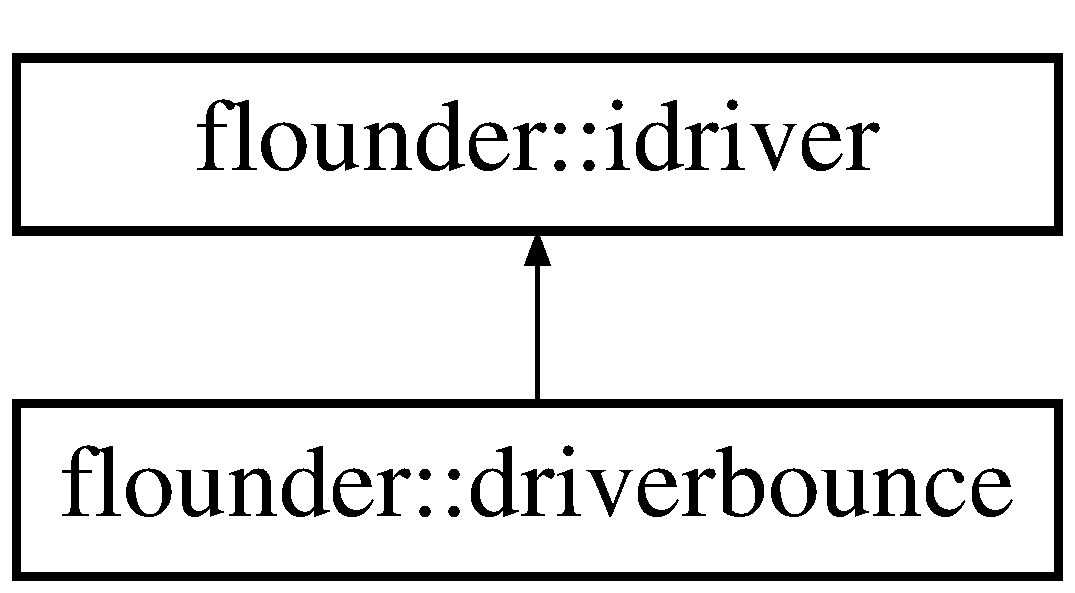
\includegraphics[height=2.000000cm]{classflounder_1_1driverbounce}
\end{center}
\end{figure}
\subsection*{Public Member Functions}
\begin{DoxyCompactItemize}
\item 
\hyperlink{classflounder_1_1driverbounce_a92651c598bb5e6b7d8d8f686fc07bcd1}{driverbounce} (const float \&start, const float \&end, const float \&length)
\begin{DoxyCompactList}\small\item\em Creates a new sine wave driver. \end{DoxyCompactList}\item 
\hyperlink{classflounder_1_1driverbounce_ae077e73f2f73847898a149a2812c3ea5}{$\sim$driverbounce} ()
\begin{DoxyCompactList}\small\item\em Deconstructor for bounce driver. \end{DoxyCompactList}\end{DoxyCompactItemize}
\subsection*{Protected Member Functions}
\begin{DoxyCompactItemize}
\item 
float \hyperlink{classflounder_1_1driverbounce_a2781832b47206849a0028ee75a4772e4}{calculate} (const float \&time) override
\begin{DoxyCompactList}\small\item\em Calculates the new value. \end{DoxyCompactList}\end{DoxyCompactItemize}
\subsection*{Private Attributes}
\begin{DoxyCompactItemize}
\item 
\mbox{\Hypertarget{classflounder_1_1driverbounce_a3227c13c05f51b7e16297a16ceaba2ce}\label{classflounder_1_1driverbounce_a3227c13c05f51b7e16297a16ceaba2ce}} 
float {\bfseries m\+\_\+start}
\item 
\mbox{\Hypertarget{classflounder_1_1driverbounce_ad1158cd9f43b9af60f40f8a974f5e369}\label{classflounder_1_1driverbounce_ad1158cd9f43b9af60f40f8a974f5e369}} 
float {\bfseries m\+\_\+amplitude}
\item 
\mbox{\Hypertarget{classflounder_1_1driverbounce_abd011916f956cd1364a1ef3c275dd733}\label{classflounder_1_1driverbounce_abd011916f956cd1364a1ef3c275dd733}} 
float {\bfseries m\+\_\+length}
\end{DoxyCompactItemize}


\subsection{Detailed Description}
A bounce driver that uses a sine wave. 



\subsection{Constructor \& Destructor Documentation}
\mbox{\Hypertarget{classflounder_1_1driverbounce_a92651c598bb5e6b7d8d8f686fc07bcd1}\label{classflounder_1_1driverbounce_a92651c598bb5e6b7d8d8f686fc07bcd1}} 
\index{flounder\+::driverbounce@{flounder\+::driverbounce}!driverbounce@{driverbounce}}
\index{driverbounce@{driverbounce}!flounder\+::driverbounce@{flounder\+::driverbounce}}
\subsubsection{\texorpdfstring{driverbounce()}{driverbounce()}}
{\footnotesize\ttfamily flounder\+::driverbounce\+::driverbounce (\begin{DoxyParamCaption}\item[{const float \&}]{start,  }\item[{const float \&}]{end,  }\item[{const float \&}]{length }\end{DoxyParamCaption})}



Creates a new sine wave driver. 


\begin{DoxyParams}{Parameters}
{\em start} & The start value. \\
\hline
{\em end} & The end value. \\
\hline
{\em length} & The length between two waves. \\
\hline
\end{DoxyParams}
\mbox{\Hypertarget{classflounder_1_1driverbounce_ae077e73f2f73847898a149a2812c3ea5}\label{classflounder_1_1driverbounce_ae077e73f2f73847898a149a2812c3ea5}} 
\index{flounder\+::driverbounce@{flounder\+::driverbounce}!````~driverbounce@{$\sim$driverbounce}}
\index{````~driverbounce@{$\sim$driverbounce}!flounder\+::driverbounce@{flounder\+::driverbounce}}
\subsubsection{\texorpdfstring{$\sim$driverbounce()}{~driverbounce()}}
{\footnotesize\ttfamily flounder\+::driverbounce\+::$\sim$driverbounce (\begin{DoxyParamCaption}{ }\end{DoxyParamCaption})}



Deconstructor for bounce driver. 



\subsection{Member Function Documentation}
\mbox{\Hypertarget{classflounder_1_1driverbounce_a2781832b47206849a0028ee75a4772e4}\label{classflounder_1_1driverbounce_a2781832b47206849a0028ee75a4772e4}} 
\index{flounder\+::driverbounce@{flounder\+::driverbounce}!calculate@{calculate}}
\index{calculate@{calculate}!flounder\+::driverbounce@{flounder\+::driverbounce}}
\subsubsection{\texorpdfstring{calculate()}{calculate()}}
{\footnotesize\ttfamily float flounder\+::driverbounce\+::calculate (\begin{DoxyParamCaption}\item[{const float \&}]{time }\end{DoxyParamCaption})\hspace{0.3cm}{\ttfamily [override]}, {\ttfamily [protected]}, {\ttfamily [virtual]}}



Calculates the new value. 


\begin{DoxyParams}{Parameters}
{\em time} & The time into the drivers life. \\
\hline
\end{DoxyParams}
\begin{DoxyReturn}{Returns}
The calculated value. 
\end{DoxyReturn}


Implements \hyperlink{classflounder_1_1idriver_a034c4159dc98c4c37ffdfaae64e4a16d}{flounder\+::idriver}.



The documentation for this class was generated from the following files\+:\begin{DoxyCompactItemize}
\item 
C\+:/\+Users/mattp/\+Documents/\+Flounder/\+Flounder\+Core/\+Sources/visual/driverbounce.\+h\item 
C\+:/\+Users/mattp/\+Documents/\+Flounder/\+Flounder\+Core/\+Sources/visual/driverbounce.\+cpp\end{DoxyCompactItemize}

\hypertarget{classflounder_1_1driverconstant}{}\section{flounder\+:\+:driverconstant Class Reference}
\label{classflounder_1_1driverconstant}\index{flounder\+::driverconstant@{flounder\+::driverconstant}}


A driver that has a constant value.  




{\ttfamily \#include $<$driverconstant.\+h$>$}

Inheritance diagram for flounder\+:\+:driverconstant\+:\begin{figure}[H]
\begin{center}
\leavevmode
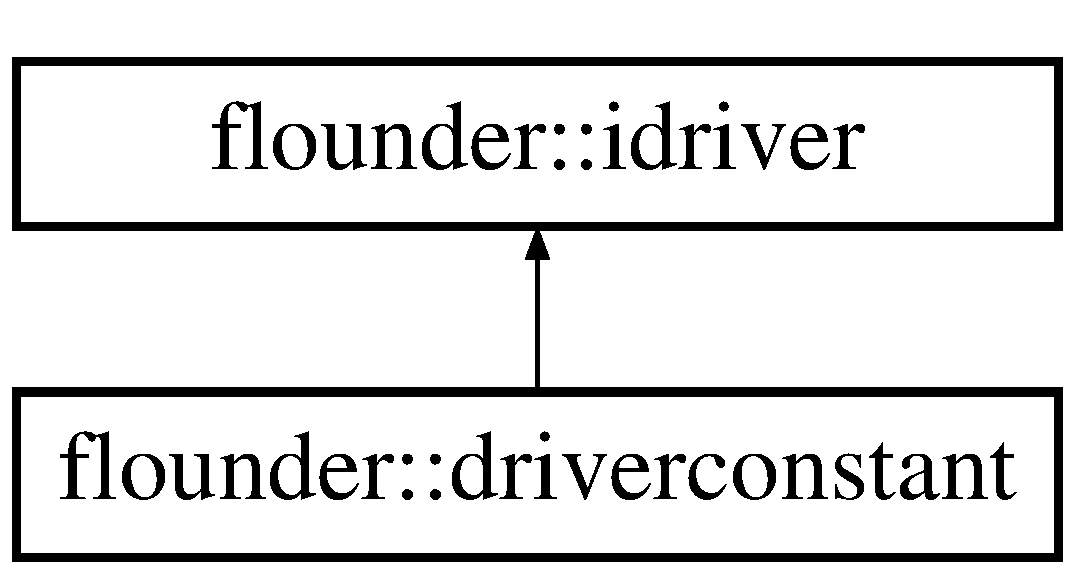
\includegraphics[height=2.000000cm]{classflounder_1_1driverconstant}
\end{center}
\end{figure}
\subsection*{Public Member Functions}
\begin{DoxyCompactItemize}
\item 
\hyperlink{classflounder_1_1driverconstant_a678370c3748065cea8fc7ca6f46c2a19}{driverconstant} (const float \&constant)
\begin{DoxyCompactList}\small\item\em Creates a new constant driver. \end{DoxyCompactList}\item 
\hyperlink{classflounder_1_1driverconstant_abedf27fbdda1f3521c15e555ba54633e}{$\sim$driverconstant} ()
\begin{DoxyCompactList}\small\item\em Deconstructor for constant driver. \end{DoxyCompactList}\end{DoxyCompactItemize}
\subsection*{Protected Member Functions}
\begin{DoxyCompactItemize}
\item 
float \hyperlink{classflounder_1_1driverconstant_acf786b61ab46ea1ebf8d9a802c33c441}{calculate} (const float \&time) override
\begin{DoxyCompactList}\small\item\em Calculates the new value. \end{DoxyCompactList}\end{DoxyCompactItemize}
\subsection*{Private Attributes}
\begin{DoxyCompactItemize}
\item 
\mbox{\Hypertarget{classflounder_1_1driverconstant_a1e02a3e81305e1caef95303ca288d20b}\label{classflounder_1_1driverconstant_a1e02a3e81305e1caef95303ca288d20b}} 
float {\bfseries m\+\_\+value}
\end{DoxyCompactItemize}


\subsection{Detailed Description}
A driver that has a constant value. 



\subsection{Constructor \& Destructor Documentation}
\mbox{\Hypertarget{classflounder_1_1driverconstant_a678370c3748065cea8fc7ca6f46c2a19}\label{classflounder_1_1driverconstant_a678370c3748065cea8fc7ca6f46c2a19}} 
\index{flounder\+::driverconstant@{flounder\+::driverconstant}!driverconstant@{driverconstant}}
\index{driverconstant@{driverconstant}!flounder\+::driverconstant@{flounder\+::driverconstant}}
\subsubsection{\texorpdfstring{driverconstant()}{driverconstant()}}
{\footnotesize\ttfamily flounder\+::driverconstant\+::driverconstant (\begin{DoxyParamCaption}\item[{const float \&}]{constant }\end{DoxyParamCaption})}



Creates a new constant driver. 


\begin{DoxyParams}{Parameters}
{\em constant} & The constant value. \\
\hline
\end{DoxyParams}
\mbox{\Hypertarget{classflounder_1_1driverconstant_abedf27fbdda1f3521c15e555ba54633e}\label{classflounder_1_1driverconstant_abedf27fbdda1f3521c15e555ba54633e}} 
\index{flounder\+::driverconstant@{flounder\+::driverconstant}!````~driverconstant@{$\sim$driverconstant}}
\index{````~driverconstant@{$\sim$driverconstant}!flounder\+::driverconstant@{flounder\+::driverconstant}}
\subsubsection{\texorpdfstring{$\sim$driverconstant()}{~driverconstant()}}
{\footnotesize\ttfamily flounder\+::driverconstant\+::$\sim$driverconstant (\begin{DoxyParamCaption}{ }\end{DoxyParamCaption})}



Deconstructor for constant driver. 



\subsection{Member Function Documentation}
\mbox{\Hypertarget{classflounder_1_1driverconstant_acf786b61ab46ea1ebf8d9a802c33c441}\label{classflounder_1_1driverconstant_acf786b61ab46ea1ebf8d9a802c33c441}} 
\index{flounder\+::driverconstant@{flounder\+::driverconstant}!calculate@{calculate}}
\index{calculate@{calculate}!flounder\+::driverconstant@{flounder\+::driverconstant}}
\subsubsection{\texorpdfstring{calculate()}{calculate()}}
{\footnotesize\ttfamily float flounder\+::driverconstant\+::calculate (\begin{DoxyParamCaption}\item[{const float \&}]{time }\end{DoxyParamCaption})\hspace{0.3cm}{\ttfamily [override]}, {\ttfamily [protected]}, {\ttfamily [virtual]}}



Calculates the new value. 


\begin{DoxyParams}{Parameters}
{\em time} & The time into the drivers life. \\
\hline
\end{DoxyParams}
\begin{DoxyReturn}{Returns}
The calculated value. 
\end{DoxyReturn}


Implements \hyperlink{classflounder_1_1idriver_a034c4159dc98c4c37ffdfaae64e4a16d}{flounder\+::idriver}.



The documentation for this class was generated from the following files\+:\begin{DoxyCompactItemize}
\item 
Flounder-\/\+Core/src/visual/driverconstant.\+h\item 
Flounder-\/\+Core/src/visual/driverconstant.\+cpp\end{DoxyCompactItemize}

\hypertarget{classflounder_1_1driverfade}{}\section{flounder\+:\+:driverfade Class Reference}
\label{classflounder_1_1driverfade}\index{flounder\+::driverfade@{flounder\+::driverfade}}


A driver that fades from start to end.  




{\ttfamily \#include $<$driverfade.\+h$>$}

Inheritance diagram for flounder\+:\+:driverfade\+:\begin{figure}[H]
\begin{center}
\leavevmode
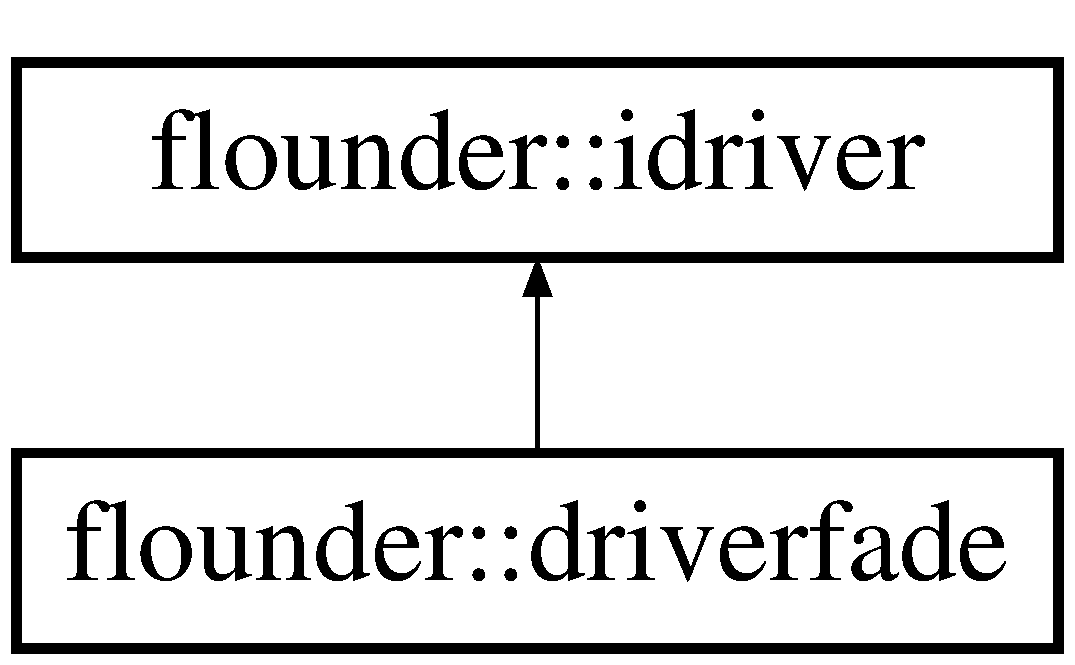
\includegraphics[height=2.000000cm]{classflounder_1_1driverfade}
\end{center}
\end{figure}
\subsection*{Public Member Functions}
\begin{DoxyCompactItemize}
\item 
\hyperlink{classflounder_1_1driverfade_a4aa6c6ec1352f9af77c218f4483896e7}{driverfade} (const float \&start, const float \&end, const float \&peak, const float \&length)
\begin{DoxyCompactList}\small\item\em Creates a new fade driver. \end{DoxyCompactList}\item 
\hyperlink{classflounder_1_1driverfade_a230478bdd0efec38ea6dd3b598676fd3}{$\sim$driverfade} ()
\begin{DoxyCompactList}\small\item\em Deconstructor for fade driver. \end{DoxyCompactList}\item 
float \& \hyperlink{classflounder_1_1driverfade_a16f5ada8b7e3708f57ec4dee87b5bd59}{get\+Start} ()
\begin{DoxyCompactList}\small\item\em Gets the start time. \end{DoxyCompactList}\item 
void \hyperlink{classflounder_1_1driverfade_a6a38fe711e23d2ee17909491721b9c5d}{set\+Start} (const float \&start)
\begin{DoxyCompactList}\small\item\em Sets the start time. \end{DoxyCompactList}\item 
float \& \hyperlink{classflounder_1_1driverfade_a8afc25faac85241befa44a3199d6aa66}{get\+End} ()
\begin{DoxyCompactList}\small\item\em Gets the end time. \end{DoxyCompactList}\item 
void \hyperlink{classflounder_1_1driverfade_aa4cec5e23d739ade9704cd09062c8e61}{set\+End} (const float \&end)
\begin{DoxyCompactList}\small\item\em Sets the end time. \end{DoxyCompactList}\item 
float \& \hyperlink{classflounder_1_1driverfade_adc6fe117b31bce8bbeb315f42238c5c7}{get\+Peak} ()
\begin{DoxyCompactList}\small\item\em Gets the peak value. \end{DoxyCompactList}\item 
void \hyperlink{classflounder_1_1driverfade_a2ef147225bc3371021ab34d24ff830c2}{set\+Peak} (const float \&peak)
\begin{DoxyCompactList}\small\item\em Sets the peak value. \end{DoxyCompactList}\end{DoxyCompactItemize}
\subsection*{Protected Member Functions}
\begin{DoxyCompactItemize}
\item 
float \hyperlink{classflounder_1_1driverfade_af0720c2a60e768dfa9702a43969bf65d}{calculate} (const float \&time) override
\begin{DoxyCompactList}\small\item\em Calculates the new value. \end{DoxyCompactList}\end{DoxyCompactItemize}
\subsection*{Private Attributes}
\begin{DoxyCompactItemize}
\item 
\mbox{\Hypertarget{classflounder_1_1driverfade_a0116d4678be3c6de69137836a066dd14}\label{classflounder_1_1driverfade_a0116d4678be3c6de69137836a066dd14}} 
float {\bfseries m\+\_\+start}
\item 
\mbox{\Hypertarget{classflounder_1_1driverfade_aedbb138185ff786053444437da900553}\label{classflounder_1_1driverfade_aedbb138185ff786053444437da900553}} 
float {\bfseries m\+\_\+end}
\item 
\mbox{\Hypertarget{classflounder_1_1driverfade_a536ef333071a5120c49553748c3046ff}\label{classflounder_1_1driverfade_a536ef333071a5120c49553748c3046ff}} 
float {\bfseries m\+\_\+peak}
\end{DoxyCompactItemize}


\subsection{Detailed Description}
A driver that fades from start to end. 



\subsection{Constructor \& Destructor Documentation}
\mbox{\Hypertarget{classflounder_1_1driverfade_a4aa6c6ec1352f9af77c218f4483896e7}\label{classflounder_1_1driverfade_a4aa6c6ec1352f9af77c218f4483896e7}} 
\index{flounder\+::driverfade@{flounder\+::driverfade}!driverfade@{driverfade}}
\index{driverfade@{driverfade}!flounder\+::driverfade@{flounder\+::driverfade}}
\subsubsection{\texorpdfstring{driverfade()}{driverfade()}}
{\footnotesize\ttfamily flounder\+::driverfade\+::driverfade (\begin{DoxyParamCaption}\item[{const float \&}]{start,  }\item[{const float \&}]{end,  }\item[{const float \&}]{peak,  }\item[{const float \&}]{length }\end{DoxyParamCaption})}



Creates a new fade driver. 


\begin{DoxyParams}{Parameters}
{\em start} & The start time. \\
\hline
{\em end} & The end time. \\
\hline
{\em peak} & The peak value. \\
\hline
{\em length} & The time taken to get to the end. \\
\hline
\end{DoxyParams}
\mbox{\Hypertarget{classflounder_1_1driverfade_a230478bdd0efec38ea6dd3b598676fd3}\label{classflounder_1_1driverfade_a230478bdd0efec38ea6dd3b598676fd3}} 
\index{flounder\+::driverfade@{flounder\+::driverfade}!````~driverfade@{$\sim$driverfade}}
\index{````~driverfade@{$\sim$driverfade}!flounder\+::driverfade@{flounder\+::driverfade}}
\subsubsection{\texorpdfstring{$\sim$driverfade()}{~driverfade()}}
{\footnotesize\ttfamily flounder\+::driverfade\+::$\sim$driverfade (\begin{DoxyParamCaption}{ }\end{DoxyParamCaption})}



Deconstructor for fade driver. 



\subsection{Member Function Documentation}
\mbox{\Hypertarget{classflounder_1_1driverfade_af0720c2a60e768dfa9702a43969bf65d}\label{classflounder_1_1driverfade_af0720c2a60e768dfa9702a43969bf65d}} 
\index{flounder\+::driverfade@{flounder\+::driverfade}!calculate@{calculate}}
\index{calculate@{calculate}!flounder\+::driverfade@{flounder\+::driverfade}}
\subsubsection{\texorpdfstring{calculate()}{calculate()}}
{\footnotesize\ttfamily float flounder\+::driverfade\+::calculate (\begin{DoxyParamCaption}\item[{const float \&}]{time }\end{DoxyParamCaption})\hspace{0.3cm}{\ttfamily [override]}, {\ttfamily [protected]}, {\ttfamily [virtual]}}



Calculates the new value. 


\begin{DoxyParams}{Parameters}
{\em time} & The time into the drivers life. \\
\hline
\end{DoxyParams}
\begin{DoxyReturn}{Returns}
The calculated value. 
\end{DoxyReturn}


Implements \hyperlink{classflounder_1_1idriver_a034c4159dc98c4c37ffdfaae64e4a16d}{flounder\+::idriver}.

\mbox{\Hypertarget{classflounder_1_1driverfade_a8afc25faac85241befa44a3199d6aa66}\label{classflounder_1_1driverfade_a8afc25faac85241befa44a3199d6aa66}} 
\index{flounder\+::driverfade@{flounder\+::driverfade}!get\+End@{get\+End}}
\index{get\+End@{get\+End}!flounder\+::driverfade@{flounder\+::driverfade}}
\subsubsection{\texorpdfstring{get\+End()}{getEnd()}}
{\footnotesize\ttfamily float\& flounder\+::driverfade\+::get\+End (\begin{DoxyParamCaption}{ }\end{DoxyParamCaption})\hspace{0.3cm}{\ttfamily [inline]}}



Gets the end time. 

\begin{DoxyReturn}{Returns}
The ebd time. 
\end{DoxyReturn}
\mbox{\Hypertarget{classflounder_1_1driverfade_adc6fe117b31bce8bbeb315f42238c5c7}\label{classflounder_1_1driverfade_adc6fe117b31bce8bbeb315f42238c5c7}} 
\index{flounder\+::driverfade@{flounder\+::driverfade}!get\+Peak@{get\+Peak}}
\index{get\+Peak@{get\+Peak}!flounder\+::driverfade@{flounder\+::driverfade}}
\subsubsection{\texorpdfstring{get\+Peak()}{getPeak()}}
{\footnotesize\ttfamily float\& flounder\+::driverfade\+::get\+Peak (\begin{DoxyParamCaption}{ }\end{DoxyParamCaption})\hspace{0.3cm}{\ttfamily [inline]}}



Gets the peak value. 

\begin{DoxyReturn}{Returns}
The peak value. 
\end{DoxyReturn}
\mbox{\Hypertarget{classflounder_1_1driverfade_a16f5ada8b7e3708f57ec4dee87b5bd59}\label{classflounder_1_1driverfade_a16f5ada8b7e3708f57ec4dee87b5bd59}} 
\index{flounder\+::driverfade@{flounder\+::driverfade}!get\+Start@{get\+Start}}
\index{get\+Start@{get\+Start}!flounder\+::driverfade@{flounder\+::driverfade}}
\subsubsection{\texorpdfstring{get\+Start()}{getStart()}}
{\footnotesize\ttfamily float\& flounder\+::driverfade\+::get\+Start (\begin{DoxyParamCaption}{ }\end{DoxyParamCaption})\hspace{0.3cm}{\ttfamily [inline]}}



Gets the start time. 

\begin{DoxyReturn}{Returns}
The start time. 
\end{DoxyReturn}
\mbox{\Hypertarget{classflounder_1_1driverfade_aa4cec5e23d739ade9704cd09062c8e61}\label{classflounder_1_1driverfade_aa4cec5e23d739ade9704cd09062c8e61}} 
\index{flounder\+::driverfade@{flounder\+::driverfade}!set\+End@{set\+End}}
\index{set\+End@{set\+End}!flounder\+::driverfade@{flounder\+::driverfade}}
\subsubsection{\texorpdfstring{set\+End()}{setEnd()}}
{\footnotesize\ttfamily void flounder\+::driverfade\+::set\+End (\begin{DoxyParamCaption}\item[{const float \&}]{end }\end{DoxyParamCaption})\hspace{0.3cm}{\ttfamily [inline]}}



Sets the end time. 


\begin{DoxyParams}{Parameters}
{\em end} & The new end time. \\
\hline
\end{DoxyParams}
\mbox{\Hypertarget{classflounder_1_1driverfade_a2ef147225bc3371021ab34d24ff830c2}\label{classflounder_1_1driverfade_a2ef147225bc3371021ab34d24ff830c2}} 
\index{flounder\+::driverfade@{flounder\+::driverfade}!set\+Peak@{set\+Peak}}
\index{set\+Peak@{set\+Peak}!flounder\+::driverfade@{flounder\+::driverfade}}
\subsubsection{\texorpdfstring{set\+Peak()}{setPeak()}}
{\footnotesize\ttfamily void flounder\+::driverfade\+::set\+Peak (\begin{DoxyParamCaption}\item[{const float \&}]{peak }\end{DoxyParamCaption})\hspace{0.3cm}{\ttfamily [inline]}}



Sets the peak value. 


\begin{DoxyParams}{Parameters}
{\em peak} & The new peak value. \\
\hline
\end{DoxyParams}
\mbox{\Hypertarget{classflounder_1_1driverfade_a6a38fe711e23d2ee17909491721b9c5d}\label{classflounder_1_1driverfade_a6a38fe711e23d2ee17909491721b9c5d}} 
\index{flounder\+::driverfade@{flounder\+::driverfade}!set\+Start@{set\+Start}}
\index{set\+Start@{set\+Start}!flounder\+::driverfade@{flounder\+::driverfade}}
\subsubsection{\texorpdfstring{set\+Start()}{setStart()}}
{\footnotesize\ttfamily void flounder\+::driverfade\+::set\+Start (\begin{DoxyParamCaption}\item[{const float \&}]{start }\end{DoxyParamCaption})\hspace{0.3cm}{\ttfamily [inline]}}



Sets the start time. 


\begin{DoxyParams}{Parameters}
{\em start} & The new start time. \\
\hline
\end{DoxyParams}


The documentation for this class was generated from the following files\+:\begin{DoxyCompactItemize}
\item 
Flounder-\/\+Core/src/visual/driverfade.\+h\item 
Flounder-\/\+Core/src/visual/driverfade.\+cpp\end{DoxyCompactItemize}

\hypertarget{classflounder_1_1driverlinear}{}\section{flounder\+:\+:driverlinear Class Reference}
\label{classflounder_1_1driverlinear}\index{flounder\+::driverlinear@{flounder\+::driverlinear}}


A driver that linearly increases its value.  




{\ttfamily \#include $<$driverlinear.\+h$>$}

Inheritance diagram for flounder\+:\+:driverlinear\+:\begin{figure}[H]
\begin{center}
\leavevmode
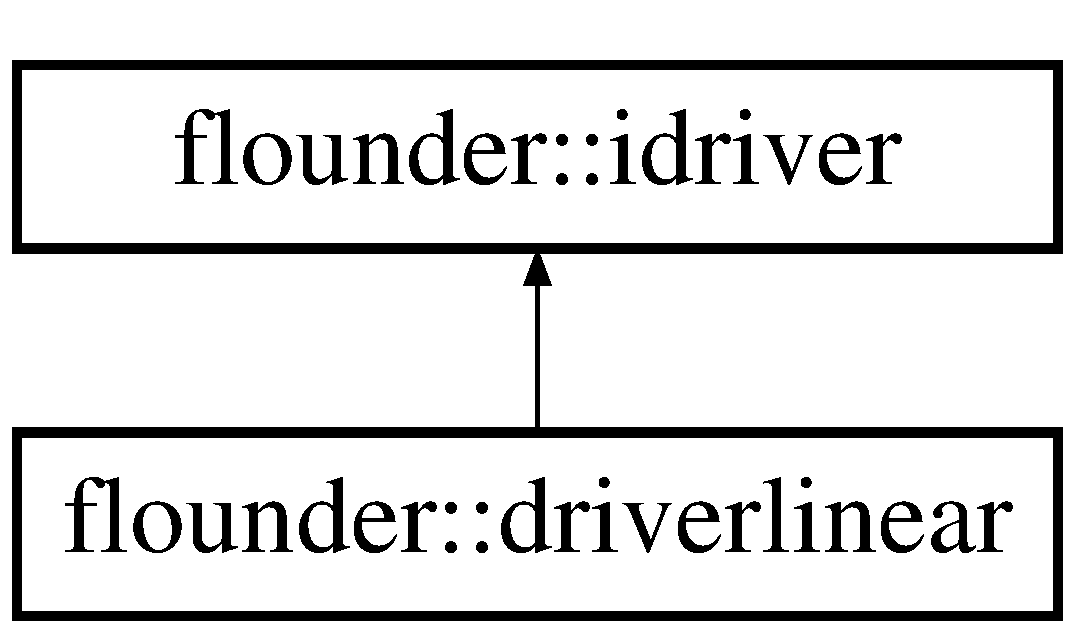
\includegraphics[height=2.000000cm]{classflounder_1_1driverlinear}
\end{center}
\end{figure}
\subsection*{Public Member Functions}
\begin{DoxyCompactItemize}
\item 
\hyperlink{classflounder_1_1driverlinear_a4644bdd0dc29e8e8129fbcd4fc2c57ed}{driverlinear} (const float \&start\+Value, const float \&end\+Value, const float \&length)
\begin{DoxyCompactList}\small\item\em Creates a new linear driver. \end{DoxyCompactList}\item 
\hyperlink{classflounder_1_1driverlinear_a792fa316601770f3d40a398618564bc6}{$\sim$driverlinear} ()
\begin{DoxyCompactList}\small\item\em Deconstructor for linear driver. \end{DoxyCompactList}\end{DoxyCompactItemize}
\subsection*{Protected Member Functions}
\begin{DoxyCompactItemize}
\item 
float \hyperlink{classflounder_1_1driverlinear_a7f645c05d7a8bdb555bbf70aca7c630e}{calculate} (const float \&time) override
\begin{DoxyCompactList}\small\item\em Calculates the new value. \end{DoxyCompactList}\end{DoxyCompactItemize}
\subsection*{Private Attributes}
\begin{DoxyCompactItemize}
\item 
\mbox{\Hypertarget{classflounder_1_1driverlinear_a0cefe5c5d951d188482856a4f46c53e7}\label{classflounder_1_1driverlinear_a0cefe5c5d951d188482856a4f46c53e7}} 
float {\bfseries m\+\_\+start\+Value}
\item 
\mbox{\Hypertarget{classflounder_1_1driverlinear_a2b76b658eaab5e39097dfcab59a62cb7}\label{classflounder_1_1driverlinear_a2b76b658eaab5e39097dfcab59a62cb7}} 
float {\bfseries m\+\_\+difference}
\end{DoxyCompactItemize}


\subsection{Detailed Description}
A driver that linearly increases its value. 



\subsection{Constructor \& Destructor Documentation}
\mbox{\Hypertarget{classflounder_1_1driverlinear_a4644bdd0dc29e8e8129fbcd4fc2c57ed}\label{classflounder_1_1driverlinear_a4644bdd0dc29e8e8129fbcd4fc2c57ed}} 
\index{flounder\+::driverlinear@{flounder\+::driverlinear}!driverlinear@{driverlinear}}
\index{driverlinear@{driverlinear}!flounder\+::driverlinear@{flounder\+::driverlinear}}
\subsubsection{\texorpdfstring{driverlinear()}{driverlinear()}}
{\footnotesize\ttfamily flounder\+::driverlinear\+::driverlinear (\begin{DoxyParamCaption}\item[{const float \&}]{start\+Value,  }\item[{const float \&}]{end\+Value,  }\item[{const float \&}]{length }\end{DoxyParamCaption})}



Creates a new linear driver. 


\begin{DoxyParams}{Parameters}
{\em start\+Value} & The start value. \\
\hline
{\em end\+Value} & The end value. \\
\hline
{\em length} & The time to go between values. \\
\hline
\end{DoxyParams}
\mbox{\Hypertarget{classflounder_1_1driverlinear_a792fa316601770f3d40a398618564bc6}\label{classflounder_1_1driverlinear_a792fa316601770f3d40a398618564bc6}} 
\index{flounder\+::driverlinear@{flounder\+::driverlinear}!````~driverlinear@{$\sim$driverlinear}}
\index{````~driverlinear@{$\sim$driverlinear}!flounder\+::driverlinear@{flounder\+::driverlinear}}
\subsubsection{\texorpdfstring{$\sim$driverlinear()}{~driverlinear()}}
{\footnotesize\ttfamily flounder\+::driverlinear\+::$\sim$driverlinear (\begin{DoxyParamCaption}{ }\end{DoxyParamCaption})}



Deconstructor for linear driver. 



\subsection{Member Function Documentation}
\mbox{\Hypertarget{classflounder_1_1driverlinear_a7f645c05d7a8bdb555bbf70aca7c630e}\label{classflounder_1_1driverlinear_a7f645c05d7a8bdb555bbf70aca7c630e}} 
\index{flounder\+::driverlinear@{flounder\+::driverlinear}!calculate@{calculate}}
\index{calculate@{calculate}!flounder\+::driverlinear@{flounder\+::driverlinear}}
\subsubsection{\texorpdfstring{calculate()}{calculate()}}
{\footnotesize\ttfamily float flounder\+::driverlinear\+::calculate (\begin{DoxyParamCaption}\item[{const float \&}]{time }\end{DoxyParamCaption})\hspace{0.3cm}{\ttfamily [override]}, {\ttfamily [protected]}, {\ttfamily [virtual]}}



Calculates the new value. 


\begin{DoxyParams}{Parameters}
{\em time} & The time into the drivers life. \\
\hline
\end{DoxyParams}
\begin{DoxyReturn}{Returns}
The calculated value. 
\end{DoxyReturn}


Implements \hyperlink{classflounder_1_1idriver_a034c4159dc98c4c37ffdfaae64e4a16d}{flounder\+::idriver}.



The documentation for this class was generated from the following files\+:\begin{DoxyCompactItemize}
\item 
C\+:/\+Users/mattp/\+Documents/\+Flounder/\+Flounder\+Core/\+Sources/visual/driverlinear.\+h\item 
C\+:/\+Users/mattp/\+Documents/\+Flounder/\+Flounder\+Core/\+Sources/visual/driverlinear.\+cpp\end{DoxyCompactItemize}

\hypertarget{classflounder_1_1driversinwave}{}\section{flounder\+:\+:driversinwave Class Reference}
\label{classflounder_1_1driversinwave}\index{flounder\+::driversinwave@{flounder\+::driversinwave}}


A driver that uses a sine wave.  




{\ttfamily \#include $<$driversinwave.\+h$>$}

Inheritance diagram for flounder\+:\+:driversinwave\+:\begin{figure}[H]
\begin{center}
\leavevmode
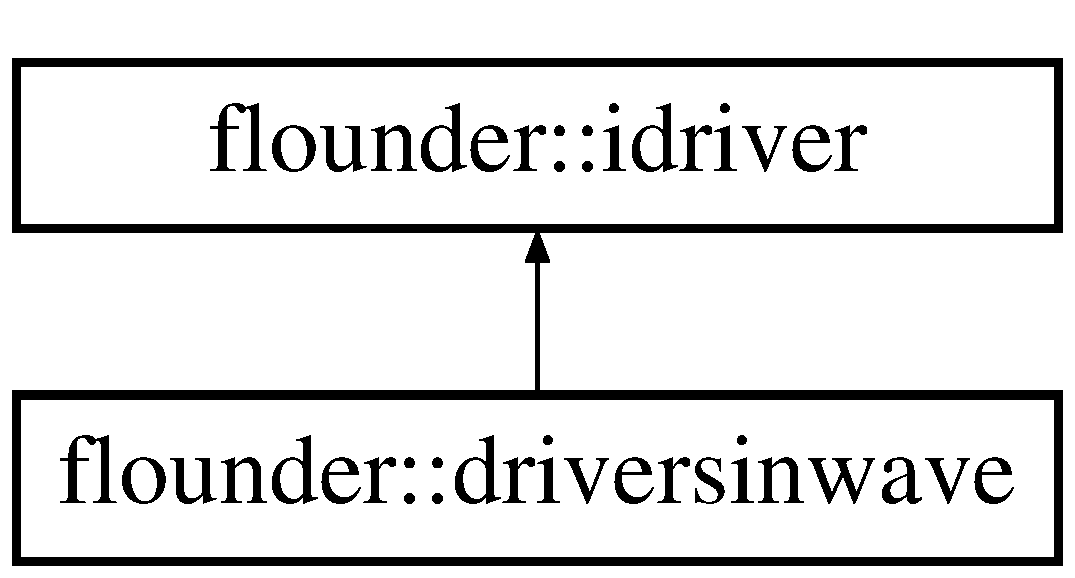
\includegraphics[height=2.000000cm]{classflounder_1_1driversinwave}
\end{center}
\end{figure}
\subsection*{Public Member Functions}
\begin{DoxyCompactItemize}
\item 
\hyperlink{classflounder_1_1driversinwave_ab076a8b6fbbb6a33e627c41a8978d5bc}{driversinwave} (const float \&min, const float \&max, const float \&length)
\begin{DoxyCompactList}\small\item\em Creates a new sine wave driver. \end{DoxyCompactList}\item 
\hyperlink{classflounder_1_1driversinwave_a6d4bc8b23f918d9f355d463fe8dee688}{$\sim$driversinwave} ()
\begin{DoxyCompactList}\small\item\em Deconstructor for sin wave driver. \end{DoxyCompactList}\end{DoxyCompactItemize}
\subsection*{Protected Member Functions}
\begin{DoxyCompactItemize}
\item 
float \hyperlink{classflounder_1_1driversinwave_ae5c3d8d4bd38082ad2b0396029d45e66}{calculate} (const float \&time) override
\begin{DoxyCompactList}\small\item\em Calculates the new value. \end{DoxyCompactList}\end{DoxyCompactItemize}
\subsection*{Private Attributes}
\begin{DoxyCompactItemize}
\item 
\mbox{\Hypertarget{classflounder_1_1driversinwave_ada1752f8316eb66bcfede70f21d77f78}\label{classflounder_1_1driversinwave_ada1752f8316eb66bcfede70f21d77f78}} 
float {\bfseries m\+\_\+min}
\item 
\mbox{\Hypertarget{classflounder_1_1driversinwave_a6b203dca1247a27a5b0befc9c5627eac}\label{classflounder_1_1driversinwave_a6b203dca1247a27a5b0befc9c5627eac}} 
float {\bfseries m\+\_\+amplitude}
\end{DoxyCompactItemize}


\subsection{Detailed Description}
A driver that uses a sine wave. 



\subsection{Constructor \& Destructor Documentation}
\mbox{\Hypertarget{classflounder_1_1driversinwave_ab076a8b6fbbb6a33e627c41a8978d5bc}\label{classflounder_1_1driversinwave_ab076a8b6fbbb6a33e627c41a8978d5bc}} 
\index{flounder\+::driversinwave@{flounder\+::driversinwave}!driversinwave@{driversinwave}}
\index{driversinwave@{driversinwave}!flounder\+::driversinwave@{flounder\+::driversinwave}}
\subsubsection{\texorpdfstring{driversinwave()}{driversinwave()}}
{\footnotesize\ttfamily flounder\+::driversinwave\+::driversinwave (\begin{DoxyParamCaption}\item[{const float \&}]{min,  }\item[{const float \&}]{max,  }\item[{const float \&}]{length }\end{DoxyParamCaption})}



Creates a new sine wave driver. 


\begin{DoxyParams}{Parameters}
{\em min} & The min value. \\
\hline
{\em max} & The max value. \\
\hline
{\em length} & The length between two waves. \\
\hline
\end{DoxyParams}
\mbox{\Hypertarget{classflounder_1_1driversinwave_a6d4bc8b23f918d9f355d463fe8dee688}\label{classflounder_1_1driversinwave_a6d4bc8b23f918d9f355d463fe8dee688}} 
\index{flounder\+::driversinwave@{flounder\+::driversinwave}!````~driversinwave@{$\sim$driversinwave}}
\index{````~driversinwave@{$\sim$driversinwave}!flounder\+::driversinwave@{flounder\+::driversinwave}}
\subsubsection{\texorpdfstring{$\sim$driversinwave()}{~driversinwave()}}
{\footnotesize\ttfamily flounder\+::driversinwave\+::$\sim$driversinwave (\begin{DoxyParamCaption}{ }\end{DoxyParamCaption})}



Deconstructor for sin wave driver. 



\subsection{Member Function Documentation}
\mbox{\Hypertarget{classflounder_1_1driversinwave_ae5c3d8d4bd38082ad2b0396029d45e66}\label{classflounder_1_1driversinwave_ae5c3d8d4bd38082ad2b0396029d45e66}} 
\index{flounder\+::driversinwave@{flounder\+::driversinwave}!calculate@{calculate}}
\index{calculate@{calculate}!flounder\+::driversinwave@{flounder\+::driversinwave}}
\subsubsection{\texorpdfstring{calculate()}{calculate()}}
{\footnotesize\ttfamily float flounder\+::driversinwave\+::calculate (\begin{DoxyParamCaption}\item[{const float \&}]{time }\end{DoxyParamCaption})\hspace{0.3cm}{\ttfamily [override]}, {\ttfamily [protected]}, {\ttfamily [virtual]}}



Calculates the new value. 


\begin{DoxyParams}{Parameters}
{\em time} & The time into the drivers life. \\
\hline
\end{DoxyParams}
\begin{DoxyReturn}{Returns}
The calculated value. 
\end{DoxyReturn}


Implements \hyperlink{classflounder_1_1idriver_a034c4159dc98c4c37ffdfaae64e4a16d}{flounder\+::idriver}.



The documentation for this class was generated from the following files\+:\begin{DoxyCompactItemize}
\item 
C\+:/\+Users/mattp/\+Documents/\+Flounder/\+Flounder\+Core/\+Sources/visual/driversinwave.\+h\item 
C\+:/\+Users/mattp/\+Documents/\+Flounder/\+Flounder\+Core/\+Sources/visual/driversinwave.\+cpp\end{DoxyCompactItemize}

\hypertarget{classflounder_1_1driverslide}{}\section{flounder\+:\+:driverslide Class Reference}
\label{classflounder_1_1driverslide}\index{flounder\+::driverslide@{flounder\+::driverslide}}


A driver that slides to its destination using cosine interpolation.  




{\ttfamily \#include $<$driverslide.\+h$>$}

Inheritance diagram for flounder\+:\+:driverslide\+:\begin{figure}[H]
\begin{center}
\leavevmode
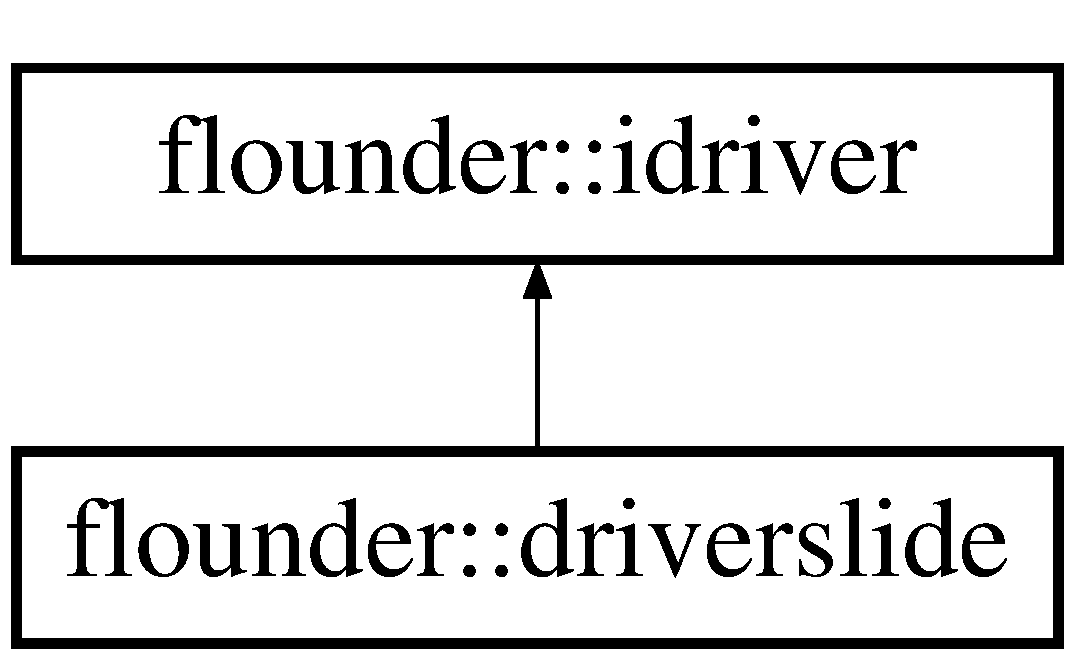
\includegraphics[height=2.000000cm]{classflounder_1_1driverslide}
\end{center}
\end{figure}
\subsection*{Public Member Functions}
\begin{DoxyCompactItemize}
\item 
\hyperlink{classflounder_1_1driverslide_a9e4b295bdb0ce7254fb7c4d7313f8b22}{driverslide} (const float \&start, const float \&end, const float \&length)
\begin{DoxyCompactList}\small\item\em Creates a new slide driver. \end{DoxyCompactList}\item 
\hyperlink{classflounder_1_1driverslide_a7972fc7a317d190a2fbfe0a0b77773e8}{$\sim$driverslide} ()
\begin{DoxyCompactList}\small\item\em Deconstructor for slide driver. \end{DoxyCompactList}\end{DoxyCompactItemize}
\subsection*{Protected Member Functions}
\begin{DoxyCompactItemize}
\item 
float \hyperlink{classflounder_1_1driverslide_aecbe9478f7ea9b1a781413f9284643c6}{calculate} (const float \&time) override
\begin{DoxyCompactList}\small\item\em Calculates the new value. \end{DoxyCompactList}\end{DoxyCompactItemize}
\subsection*{Private Attributes}
\begin{DoxyCompactItemize}
\item 
\mbox{\Hypertarget{classflounder_1_1driverslide_a649f67c646303f4e870628eee498b266}\label{classflounder_1_1driverslide_a649f67c646303f4e870628eee498b266}} 
float {\bfseries m\+\_\+start}
\item 
\mbox{\Hypertarget{classflounder_1_1driverslide_a836d4e6bd463aaed8eb253cf12b78161}\label{classflounder_1_1driverslide_a836d4e6bd463aaed8eb253cf12b78161}} 
float {\bfseries m\+\_\+end}
\item 
\mbox{\Hypertarget{classflounder_1_1driverslide_a1c4222bdf18d8ff1174ed26163f81e19}\label{classflounder_1_1driverslide_a1c4222bdf18d8ff1174ed26163f81e19}} 
float {\bfseries m\+\_\+max}
\item 
\mbox{\Hypertarget{classflounder_1_1driverslide_a31c9d82469df7e5eaa2c2de1565ae12f}\label{classflounder_1_1driverslide_a31c9d82469df7e5eaa2c2de1565ae12f}} 
bool {\bfseries m\+\_\+reached\+Target}
\end{DoxyCompactItemize}


\subsection{Detailed Description}
A driver that slides to its destination using cosine interpolation. 



\subsection{Constructor \& Destructor Documentation}
\mbox{\Hypertarget{classflounder_1_1driverslide_a9e4b295bdb0ce7254fb7c4d7313f8b22}\label{classflounder_1_1driverslide_a9e4b295bdb0ce7254fb7c4d7313f8b22}} 
\index{flounder\+::driverslide@{flounder\+::driverslide}!driverslide@{driverslide}}
\index{driverslide@{driverslide}!flounder\+::driverslide@{flounder\+::driverslide}}
\subsubsection{\texorpdfstring{driverslide()}{driverslide()}}
{\footnotesize\ttfamily flounder\+::driverslide\+::driverslide (\begin{DoxyParamCaption}\item[{const float \&}]{start,  }\item[{const float \&}]{end,  }\item[{const float \&}]{length }\end{DoxyParamCaption})}



Creates a new slide driver. 


\begin{DoxyParams}{Parameters}
{\em start} & The start value. \\
\hline
{\em end} & The end value. \\
\hline
{\em length} & The time to get to the end value. \\
\hline
\end{DoxyParams}
\mbox{\Hypertarget{classflounder_1_1driverslide_a7972fc7a317d190a2fbfe0a0b77773e8}\label{classflounder_1_1driverslide_a7972fc7a317d190a2fbfe0a0b77773e8}} 
\index{flounder\+::driverslide@{flounder\+::driverslide}!````~driverslide@{$\sim$driverslide}}
\index{````~driverslide@{$\sim$driverslide}!flounder\+::driverslide@{flounder\+::driverslide}}
\subsubsection{\texorpdfstring{$\sim$driverslide()}{~driverslide()}}
{\footnotesize\ttfamily flounder\+::driverslide\+::$\sim$driverslide (\begin{DoxyParamCaption}{ }\end{DoxyParamCaption})}



Deconstructor for slide driver. 



\subsection{Member Function Documentation}
\mbox{\Hypertarget{classflounder_1_1driverslide_aecbe9478f7ea9b1a781413f9284643c6}\label{classflounder_1_1driverslide_aecbe9478f7ea9b1a781413f9284643c6}} 
\index{flounder\+::driverslide@{flounder\+::driverslide}!calculate@{calculate}}
\index{calculate@{calculate}!flounder\+::driverslide@{flounder\+::driverslide}}
\subsubsection{\texorpdfstring{calculate()}{calculate()}}
{\footnotesize\ttfamily float flounder\+::driverslide\+::calculate (\begin{DoxyParamCaption}\item[{const float \&}]{time }\end{DoxyParamCaption})\hspace{0.3cm}{\ttfamily [override]}, {\ttfamily [protected]}, {\ttfamily [virtual]}}



Calculates the new value. 


\begin{DoxyParams}{Parameters}
{\em time} & The time into the drivers life. \\
\hline
\end{DoxyParams}
\begin{DoxyReturn}{Returns}
The calculated value. 
\end{DoxyReturn}


Implements \hyperlink{classflounder_1_1idriver_a034c4159dc98c4c37ffdfaae64e4a16d}{flounder\+::idriver}.



The documentation for this class was generated from the following files\+:\begin{DoxyCompactItemize}
\item 
Flounder-\/\+Core/src/visual/driverslide.\+h\item 
Flounder-\/\+Core/src/visual/driverslide.\+cpp\end{DoxyCompactItemize}

\hypertarget{classflounder_1_1entity}{}\section{flounder\+:\+:entity Class Reference}
\label{classflounder_1_1entity}\index{flounder\+::entity@{flounder\+::entity}}
Inheritance diagram for flounder\+:\+:entity\+:\begin{figure}[H]
\begin{center}
\leavevmode
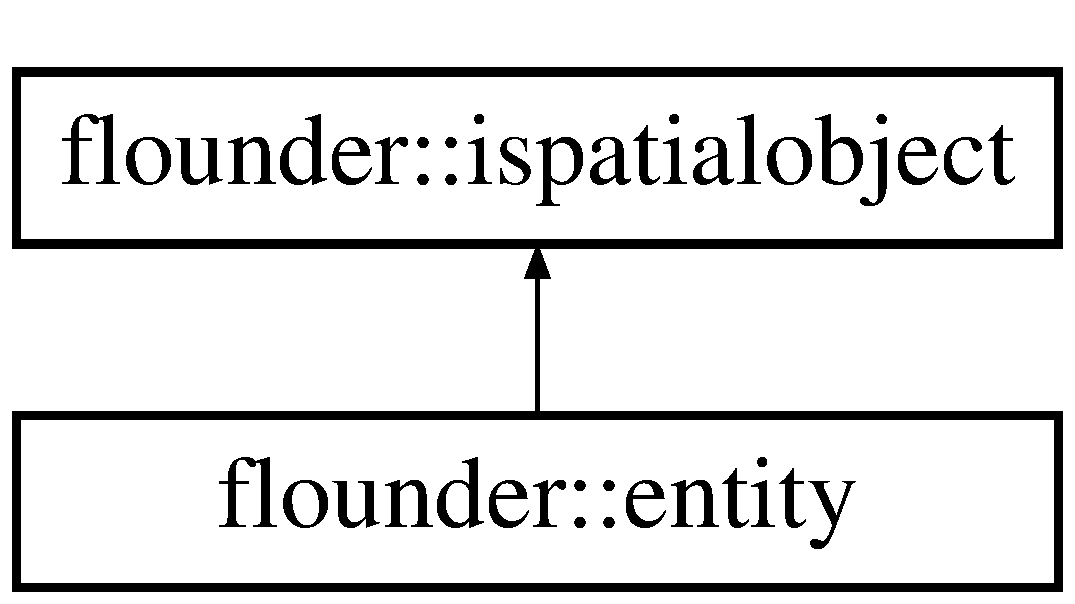
\includegraphics[height=2.000000cm]{classflounder_1_1entity}
\end{center}
\end{figure}
\subsection*{Public Member Functions}
\begin{DoxyCompactItemize}
\item 
\mbox{\Hypertarget{classflounder_1_1entity_ab5e894ac7f8af499b80435feaaf04e7e}\label{classflounder_1_1entity_ab5e894ac7f8af499b80435feaaf04e7e}} 
{\bfseries entity} (\hyperlink{classflounder_1_1ispatialstructure}{ispatialstructure}$<$ \hyperlink{classflounder_1_1entity}{entity} $\ast$$>$ $\ast$structure, const \hyperlink{classflounder_1_1vector3}{vector3} \&position, const \hyperlink{classflounder_1_1vector3}{vector3} \&rotation)
\item 
\mbox{\Hypertarget{classflounder_1_1entity_a564006c147b9f045e859855fcf40eeb2}\label{classflounder_1_1entity_a564006c147b9f045e859855fcf40eeb2}} 
void {\bfseries update} ()
\item 
\mbox{\Hypertarget{classflounder_1_1entity_a3e91898605312543c7d7620c6dc2421c}\label{classflounder_1_1entity_a3e91898605312543c7d7620c6dc2421c}} 
\hyperlink{classflounder_1_1ispatialstructure}{ispatialstructure}$<$ \hyperlink{classflounder_1_1entity}{entity} $\ast$ $>$ $\ast$ {\bfseries get\+Structure} () const
\item 
\mbox{\Hypertarget{classflounder_1_1entity_ab0bc93832ee10ebec9b348ed8584e4aa}\label{classflounder_1_1entity_ab0bc93832ee10ebec9b348ed8584e4aa}} 
void {\bfseries move\+Structure} (\hyperlink{classflounder_1_1ispatialstructure}{ispatialstructure}$<$ \hyperlink{classflounder_1_1entity}{entity} $\ast$$>$ $\ast$structure)
\item 
\mbox{\Hypertarget{classflounder_1_1entity_ab69b6b662d793755b530bb104a8c3bdb}\label{classflounder_1_1entity_ab69b6b662d793755b530bb104a8c3bdb}} 
std\+::vector$<$ \hyperlink{classflounder_1_1icomponent}{icomponent} $\ast$ $>$ $\ast$ {\bfseries get\+Components} () const
\item 
\mbox{\Hypertarget{classflounder_1_1entity_ab156e98ffc4df6fb39e53c7c89aa3b68}\label{classflounder_1_1entity_ab156e98ffc4df6fb39e53c7c89aa3b68}} 
void {\bfseries add\+Component} (\hyperlink{classflounder_1_1icomponent}{icomponent} $\ast$component)
\item 
\mbox{\Hypertarget{classflounder_1_1entity_a5a50d7de50e101cef703134bc1dc8e07}\label{classflounder_1_1entity_a5a50d7de50e101cef703134bc1dc8e07}} 
void {\bfseries remove\+Component} (\hyperlink{classflounder_1_1icomponent}{icomponent} $\ast$component)
\item 
\mbox{\Hypertarget{classflounder_1_1entity_a2481381940b2ac5f90d7287d3075b641}\label{classflounder_1_1entity_a2481381940b2ac5f90d7287d3075b641}} 
{\footnotesize template$<$class t $>$ }\\t {\bfseries get\+Component} ()
\item 
\mbox{\Hypertarget{classflounder_1_1entity_ab842d65a56e014a959e380630dd6101f}\label{classflounder_1_1entity_ab842d65a56e014a959e380630dd6101f}} 
\hyperlink{classflounder_1_1vector3}{vector3} $\ast$ {\bfseries get\+Position} () const
\item 
\mbox{\Hypertarget{classflounder_1_1entity_a49ff005d090537ecc5c2076a0efc4edb}\label{classflounder_1_1entity_a49ff005d090537ecc5c2076a0efc4edb}} 
void {\bfseries set\+Position} (const \hyperlink{classflounder_1_1vector3}{vector3} \&position) const
\item 
\mbox{\Hypertarget{classflounder_1_1entity_a8db4d74b48b21f4d7d568d846f2dea9d}\label{classflounder_1_1entity_a8db4d74b48b21f4d7d568d846f2dea9d}} 
\hyperlink{classflounder_1_1vector3}{vector3} $\ast$ {\bfseries get\+Rotation} () const
\item 
\mbox{\Hypertarget{classflounder_1_1entity_a028a111d308df2a7a358abce958452cb}\label{classflounder_1_1entity_a028a111d308df2a7a358abce958452cb}} 
void {\bfseries set\+Rotation} (const \hyperlink{classflounder_1_1vector3}{vector3} \&rotation) const
\item 
\mbox{\Hypertarget{classflounder_1_1entity_aa4ea354b1ff487a4d3a7bf760582b0da}\label{classflounder_1_1entity_aa4ea354b1ff487a4d3a7bf760582b0da}} 
bool {\bfseries get\+Removed} () const
\item 
\mbox{\Hypertarget{classflounder_1_1entity_a07a7f8bc2c53dad4ae43a3ed896000c0}\label{classflounder_1_1entity_a07a7f8bc2c53dad4ae43a3ed896000c0}} 
void {\bfseries remove} ()
\item 
\hyperlink{classflounder_1_1icollider}{icollider} $\ast$ \hyperlink{classflounder_1_1entity_a4b68d0d58f2ff338058a2fa0d1a2e413}{get\+Collider} () override
\begin{DoxyCompactList}\small\item\em Gets the shape that fully encloses the object. \end{DoxyCompactList}\end{DoxyCompactItemize}
\subsection*{Private Attributes}
\begin{DoxyCompactItemize}
\item 
\mbox{\Hypertarget{classflounder_1_1entity_ad6338e7f569238791e0787f80ce4d044}\label{classflounder_1_1entity_ad6338e7f569238791e0787f80ce4d044}} 
\hyperlink{classflounder_1_1ispatialstructure}{ispatialstructure}$<$ \hyperlink{classflounder_1_1entity}{entity} $\ast$ $>$ $\ast$ {\bfseries m\+\_\+structure}
\item 
\mbox{\Hypertarget{classflounder_1_1entity_a36bcdd06adf0aecdc01c934f7534fa91}\label{classflounder_1_1entity_a36bcdd06adf0aecdc01c934f7534fa91}} 
std\+::vector$<$ \hyperlink{classflounder_1_1icomponent}{icomponent} $\ast$ $>$ $\ast$ {\bfseries m\+\_\+components}
\item 
\mbox{\Hypertarget{classflounder_1_1entity_a8d81338fb3d84ede47cbc7695214a0d4}\label{classflounder_1_1entity_a8d81338fb3d84ede47cbc7695214a0d4}} 
\hyperlink{classflounder_1_1vector3}{vector3} $\ast$ {\bfseries m\+\_\+position}
\item 
\mbox{\Hypertarget{classflounder_1_1entity_a4d3cc88b2221b32a2f2bb97d5516957c}\label{classflounder_1_1entity_a4d3cc88b2221b32a2f2bb97d5516957c}} 
\hyperlink{classflounder_1_1vector3}{vector3} $\ast$ {\bfseries m\+\_\+rotation}
\item 
\mbox{\Hypertarget{classflounder_1_1entity_a3bf7f18a136b121b8a13c3e1226df416}\label{classflounder_1_1entity_a3bf7f18a136b121b8a13c3e1226df416}} 
bool {\bfseries m\+\_\+removed}
\end{DoxyCompactItemize}


\subsection{Member Function Documentation}
\mbox{\Hypertarget{classflounder_1_1entity_a4b68d0d58f2ff338058a2fa0d1a2e413}\label{classflounder_1_1entity_a4b68d0d58f2ff338058a2fa0d1a2e413}} 
\index{flounder\+::entity@{flounder\+::entity}!get\+Collider@{get\+Collider}}
\index{get\+Collider@{get\+Collider}!flounder\+::entity@{flounder\+::entity}}
\subsubsection{\texorpdfstring{get\+Collider()}{getCollider()}}
{\footnotesize\ttfamily \hyperlink{classflounder_1_1icollider}{icollider} $\ast$ flounder\+::entity\+::get\+Collider (\begin{DoxyParamCaption}{ }\end{DoxyParamCaption})\hspace{0.3cm}{\ttfamily [override]}, {\ttfamily [virtual]}}



Gets the shape that fully encloses the object. 

\begin{DoxyReturn}{Returns}
Returns a shape fully enclosing the object. 
\end{DoxyReturn}


Implements \hyperlink{classflounder_1_1ispatialobject_af3867cbb5f35b0296a16af77703e6c81}{flounder\+::ispatialobject}.



The documentation for this class was generated from the following files\+:\begin{DoxyCompactItemize}
\item 
Flounder-\/\+Core/src/entities/entity.\+h\item 
Flounder-\/\+Core/src/entities/entity.\+cpp\end{DoxyCompactItemize}

\hypertarget{structflounder_1_1entityrender}{}\section{flounder\+:\+:entityrender Struct Reference}
\label{structflounder_1_1entityrender}\index{flounder\+::entityrender@{flounder\+::entityrender}}
\subsection*{Public Member Functions}
\begin{DoxyCompactItemize}
\item 
\mbox{\Hypertarget{structflounder_1_1entityrender_a0d1f261c565e5e86d28448734a12111f}\label{structflounder_1_1entityrender_a0d1f261c565e5e86d28448734a12111f}} 
{\bfseries entityrender} (\hyperlink{classflounder_1_1shader}{shader} $\ast$\hyperlink{classflounder_1_1shader}{shader}, \hyperlink{classflounder_1_1model}{model} $\ast$\hyperlink{classflounder_1_1model}{model}, const bool \&shadow\+Run)
\end{DoxyCompactItemize}
\subsection*{Public Attributes}
\begin{DoxyCompactItemize}
\item 
\mbox{\Hypertarget{structflounder_1_1entityrender_adaaf488215b0798d241de923d8f1bc22}\label{structflounder_1_1entityrender_adaaf488215b0798d241de923d8f1bc22}} 
\hyperlink{classflounder_1_1shader}{shader} $\ast$ {\bfseries m\+\_\+shader}
\item 
\mbox{\Hypertarget{structflounder_1_1entityrender_aadcffd8cb210169c87833c4b335d39a4}\label{structflounder_1_1entityrender_aadcffd8cb210169c87833c4b335d39a4}} 
\hyperlink{classflounder_1_1model}{model} $\ast$ {\bfseries m\+\_\+model}
\item 
\mbox{\Hypertarget{structflounder_1_1entityrender_ad82f38909903807774d7715c2db2ab2a}\label{structflounder_1_1entityrender_ad82f38909903807774d7715c2db2ab2a}} 
bool {\bfseries m\+\_\+shadow\+Run}
\item 
\mbox{\Hypertarget{structflounder_1_1entityrender_a6d0a02d6c97834d50c59d7bcccfd34c7}\label{structflounder_1_1entityrender_a6d0a02d6c97834d50c59d7bcccfd34c7}} 
bool {\bfseries m\+\_\+undoing}
\end{DoxyCompactItemize}


The documentation for this struct was generated from the following file\+:\begin{DoxyCompactItemize}
\item 
Flounder-\/\+Core/src/entities/entityrender.\+h\end{DoxyCompactItemize}

\hypertarget{classflounder_1_1eventchange}{}\section{flounder\+:\+:eventchange$<$ t $>$ Class Template Reference}
\label{classflounder_1_1eventchange}\index{flounder\+::eventchange$<$ t $>$@{flounder\+::eventchange$<$ t $>$}}


A class that acts as a basic change listener for a value.  




{\ttfamily \#include $<$eventchange.\+h$>$}

Inheritance diagram for flounder\+:\+:eventchange$<$ t $>$\+:\begin{figure}[H]
\begin{center}
\leavevmode
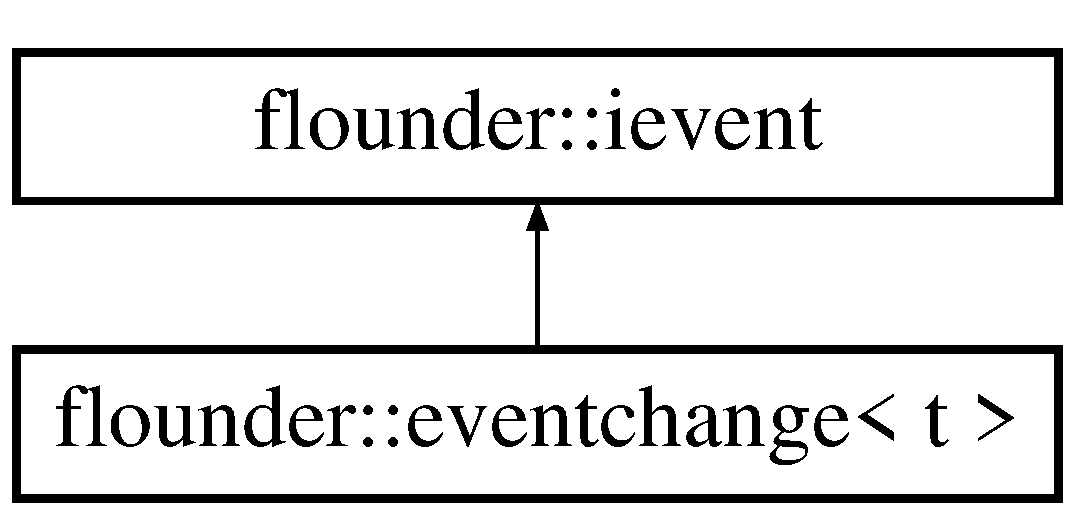
\includegraphics[height=2.000000cm]{classflounder_1_1eventchange}
\end{center}
\end{figure}
\subsection*{Public Member Functions}
\begin{DoxyCompactItemize}
\item 
\hyperlink{classflounder_1_1eventchange_aa10438da0bf89531d04211ede12f2ce1}{eventchange} (t $\ast$reference, const std\+::function$<$ void()$>$ \&\hyperlink{classflounder_1_1eventchange_aa4fd4c3c28ac6927c3a810c8775f232d}{on\+Event})
\begin{DoxyCompactList}\small\item\em Creates a new change event. \end{DoxyCompactList}\item 
bool \hyperlink{classflounder_1_1eventchange_a2ae3c1f7ae4342dfff2aae6f11b0b413}{event\+Triggered} () override
\begin{DoxyCompactList}\small\item\em Gets if the event has occurred. \end{DoxyCompactList}\item 
void \hyperlink{classflounder_1_1eventchange_aa4fd4c3c28ac6927c3a810c8775f232d}{on\+Event} () override
\begin{DoxyCompactList}\small\item\em Run when a event has occurred. \end{DoxyCompactList}\item 
bool \hyperlink{classflounder_1_1eventchange_ab3d476ecb51140e93886dc320ee44c33}{remove\+After\+Event} () override
\begin{DoxyCompactList}\small\item\em Gets if the event is removed after it has run once. \end{DoxyCompactList}\end{DoxyCompactItemize}
\subsection*{Private Attributes}
\begin{DoxyCompactItemize}
\item 
\mbox{\Hypertarget{classflounder_1_1eventchange_afdea8ccaaa60b91bbe3c7a9f289d846b}\label{classflounder_1_1eventchange_afdea8ccaaa60b91bbe3c7a9f289d846b}} 
t $\ast$ {\bfseries m\+\_\+reference}
\item 
\mbox{\Hypertarget{classflounder_1_1eventchange_a16b6829e51279a681619cdb2efbd1075}\label{classflounder_1_1eventchange_a16b6829e51279a681619cdb2efbd1075}} 
t {\bfseries m\+\_\+current}
\item 
\mbox{\Hypertarget{classflounder_1_1eventchange_ae2631399c18c52ffb7a61f65922609d3}\label{classflounder_1_1eventchange_ae2631399c18c52ffb7a61f65922609d3}} 
std\+::function$<$ void()$>$ {\bfseries m\+\_\+on\+Event}
\end{DoxyCompactItemize}


\subsection{Detailed Description}
\subsubsection*{template$<$typename t$>$\newline
class flounder\+::eventchange$<$ t $>$}

A class that acts as a basic change listener for a value. 


\begin{DoxyParams}{Parameters}
{\em $<$\+T$>$} & The type of value to find change with. \\
\hline
\end{DoxyParams}


\subsection{Constructor \& Destructor Documentation}
\mbox{\Hypertarget{classflounder_1_1eventchange_aa10438da0bf89531d04211ede12f2ce1}\label{classflounder_1_1eventchange_aa10438da0bf89531d04211ede12f2ce1}} 
\index{flounder\+::eventchange@{flounder\+::eventchange}!eventchange@{eventchange}}
\index{eventchange@{eventchange}!flounder\+::eventchange@{flounder\+::eventchange}}
\subsubsection{\texorpdfstring{eventchange()}{eventchange()}}
{\footnotesize\ttfamily template$<$typename t $>$ \\
\hyperlink{classflounder_1_1eventchange}{flounder\+::eventchange}$<$ t $>$\+::\hyperlink{classflounder_1_1eventchange}{eventchange} (\begin{DoxyParamCaption}\item[{t $\ast$}]{reference,  }\item[{const std\+::function$<$ void()$>$ \&}]{on\+Event }\end{DoxyParamCaption})}



Creates a new change event. 


\begin{DoxyParams}{Parameters}
{\em reference} & The reference to listen to. \\
\hline
{\em on\+Event} & A function called when the event is triggered. \\
\hline
\end{DoxyParams}


\subsection{Member Function Documentation}
\mbox{\Hypertarget{classflounder_1_1eventchange_a2ae3c1f7ae4342dfff2aae6f11b0b413}\label{classflounder_1_1eventchange_a2ae3c1f7ae4342dfff2aae6f11b0b413}} 
\index{flounder\+::eventchange@{flounder\+::eventchange}!event\+Triggered@{event\+Triggered}}
\index{event\+Triggered@{event\+Triggered}!flounder\+::eventchange@{flounder\+::eventchange}}
\subsubsection{\texorpdfstring{event\+Triggered()}{eventTriggered()}}
{\footnotesize\ttfamily template$<$typename t $>$ \\
bool \hyperlink{classflounder_1_1eventchange}{flounder\+::eventchange}$<$ t $>$\+::event\+Triggered (\begin{DoxyParamCaption}{ }\end{DoxyParamCaption})\hspace{0.3cm}{\ttfamily [override]}, {\ttfamily [virtual]}}



Gets if the event has occurred. 

\begin{DoxyReturn}{Returns}
The event has occurred. 
\end{DoxyReturn}


Implements \hyperlink{classflounder_1_1ievent_a4462f66feef99ef4e3521c00f4edd0c9}{flounder\+::ievent}.

\mbox{\Hypertarget{classflounder_1_1eventchange_aa4fd4c3c28ac6927c3a810c8775f232d}\label{classflounder_1_1eventchange_aa4fd4c3c28ac6927c3a810c8775f232d}} 
\index{flounder\+::eventchange@{flounder\+::eventchange}!on\+Event@{on\+Event}}
\index{on\+Event@{on\+Event}!flounder\+::eventchange@{flounder\+::eventchange}}
\subsubsection{\texorpdfstring{on\+Event()}{onEvent()}}
{\footnotesize\ttfamily template$<$typename t $>$ \\
void \hyperlink{classflounder_1_1eventchange}{flounder\+::eventchange}$<$ t $>$\+::on\+Event (\begin{DoxyParamCaption}{ }\end{DoxyParamCaption})\hspace{0.3cm}{\ttfamily [inline]}, {\ttfamily [override]}, {\ttfamily [virtual]}}



Run when a event has occurred. 



Implements \hyperlink{classflounder_1_1ievent_a6c6abe67435870b25eccd57a251a8992}{flounder\+::ievent}.

\mbox{\Hypertarget{classflounder_1_1eventchange_ab3d476ecb51140e93886dc320ee44c33}\label{classflounder_1_1eventchange_ab3d476ecb51140e93886dc320ee44c33}} 
\index{flounder\+::eventchange@{flounder\+::eventchange}!remove\+After\+Event@{remove\+After\+Event}}
\index{remove\+After\+Event@{remove\+After\+Event}!flounder\+::eventchange@{flounder\+::eventchange}}
\subsubsection{\texorpdfstring{remove\+After\+Event()}{removeAfterEvent()}}
{\footnotesize\ttfamily template$<$typename t $>$ \\
bool \hyperlink{classflounder_1_1eventchange}{flounder\+::eventchange}$<$ t $>$\+::remove\+After\+Event (\begin{DoxyParamCaption}{ }\end{DoxyParamCaption})\hspace{0.3cm}{\ttfamily [inline]}, {\ttfamily [override]}, {\ttfamily [virtual]}}



Gets if the event is removed after it has run once. 

\begin{DoxyReturn}{Returns}
If the even will run. 
\end{DoxyReturn}


Implements \hyperlink{classflounder_1_1ievent_a7017c8803df2397758980cb61020e801}{flounder\+::ievent}.



The documentation for this class was generated from the following files\+:\begin{DoxyCompactItemize}
\item 
Flounder-\/\+Core/src/events/eventchange.\+h\item 
Flounder-\/\+Core/src/events/eventchange.\+cpp\end{DoxyCompactItemize}

\hypertarget{classflounder_1_1events}{}\section{flounder\+:\+:events Class Reference}
\label{classflounder_1_1events}\index{flounder\+::events@{flounder\+::events}}


A module used for managing events on framework updates.  




{\ttfamily \#include $<$events.\+h$>$}

Inheritance diagram for flounder\+:\+:events\+:\begin{figure}[H]
\begin{center}
\leavevmode
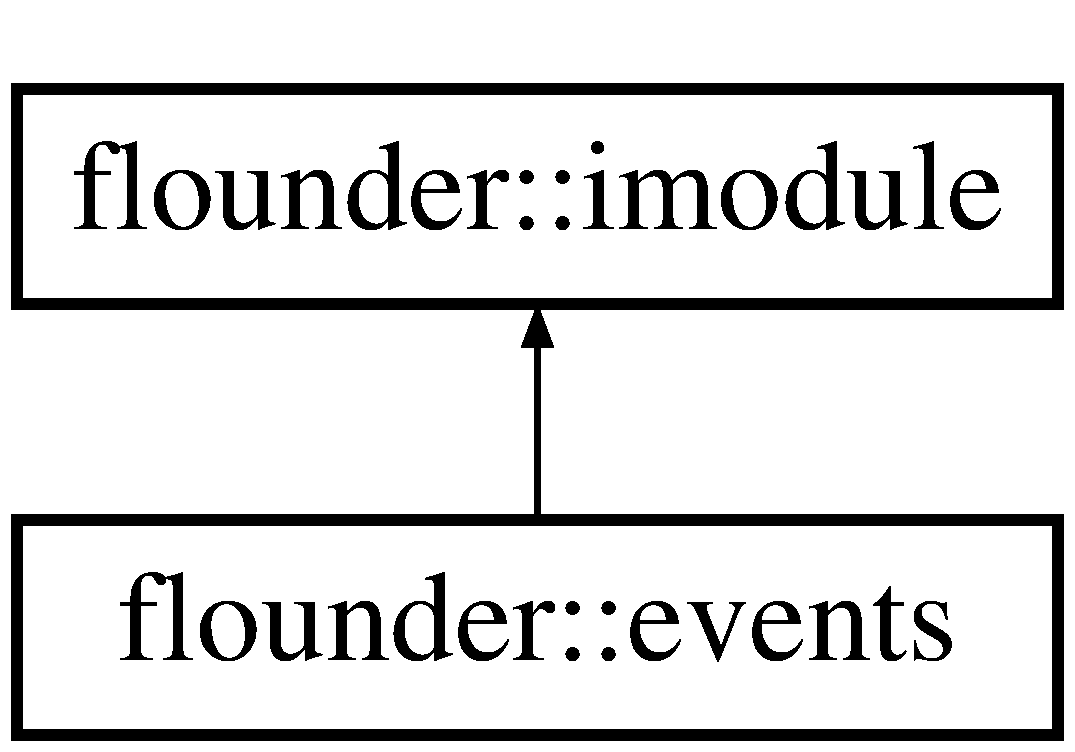
\includegraphics[height=2.000000cm]{classflounder_1_1events}
\end{center}
\end{figure}
\subsection*{Public Member Functions}
\begin{DoxyCompactItemize}
\item 
\hyperlink{classflounder_1_1events_ae354f15876d95e28706b1d96dcd790af}{events} ()
\begin{DoxyCompactList}\small\item\em Creates a new event manager. \end{DoxyCompactList}\item 
\hyperlink{classflounder_1_1events_aaf446dc74703b8ce1c04f5cf8cb06eed}{$\sim$events} ()
\begin{DoxyCompactList}\small\item\em Deconstructor for events. \end{DoxyCompactList}\item 
\mbox{\Hypertarget{classflounder_1_1events_ad51c30a5d072275fb54fad357bf763c7}\label{classflounder_1_1events_ad51c30a5d072275fb54fad357bf763c7}} 
void {\bfseries init} ()
\item 
\mbox{\Hypertarget{classflounder_1_1events_ac9735bc63eeda2d2af17586abbb5b95a}\label{classflounder_1_1events_ac9735bc63eeda2d2af17586abbb5b95a}} 
void {\bfseries update} ()
\item 
void \hyperlink{classflounder_1_1events_a6cb8ff41cf2fbf6a92ca78c122f07eb9}{add\+Event} (\hyperlink{classflounder_1_1ievent}{ievent} $\ast$event)
\begin{DoxyCompactList}\small\item\em Adds an event to the listening list. \end{DoxyCompactList}\item 
void \hyperlink{classflounder_1_1events_a957a88d282b2caa50cc87bbe039de095}{remove\+Event} (\hyperlink{classflounder_1_1ievent}{ievent} $\ast$event)
\begin{DoxyCompactList}\small\item\em Removes a event to the listening list. \end{DoxyCompactList}\end{DoxyCompactItemize}
\subsection*{Static Public Member Functions}
\begin{DoxyCompactItemize}
\item 
\mbox{\Hypertarget{classflounder_1_1events_aba09dc039ab9ddb860932a3f8d964f1e}\label{classflounder_1_1events_aba09dc039ab9ddb860932a3f8d964f1e}} 
static \hyperlink{classflounder_1_1events}{events} $\ast$ {\bfseries get} ()
\end{DoxyCompactItemize}
\subsection*{Private Attributes}
\begin{DoxyCompactItemize}
\item 
\mbox{\Hypertarget{classflounder_1_1events_ad6bb57d0e1858c5426cf9f466abc7253}\label{classflounder_1_1events_ad6bb57d0e1858c5426cf9f466abc7253}} 
std\+::vector$<$ \hyperlink{classflounder_1_1ievent}{ievent} $\ast$ $>$ $\ast$ {\bfseries m\+\_\+events}
\end{DoxyCompactItemize}


\subsection{Detailed Description}
A module used for managing events on framework updates. 



\subsection{Constructor \& Destructor Documentation}
\mbox{\Hypertarget{classflounder_1_1events_ae354f15876d95e28706b1d96dcd790af}\label{classflounder_1_1events_ae354f15876d95e28706b1d96dcd790af}} 
\index{flounder\+::events@{flounder\+::events}!events@{events}}
\index{events@{events}!flounder\+::events@{flounder\+::events}}
\subsubsection{\texorpdfstring{events()}{events()}}
{\footnotesize\ttfamily flounder\+::events\+::events (\begin{DoxyParamCaption}{ }\end{DoxyParamCaption})}



Creates a new event manager. 

\mbox{\Hypertarget{classflounder_1_1events_aaf446dc74703b8ce1c04f5cf8cb06eed}\label{classflounder_1_1events_aaf446dc74703b8ce1c04f5cf8cb06eed}} 
\index{flounder\+::events@{flounder\+::events}!````~events@{$\sim$events}}
\index{````~events@{$\sim$events}!flounder\+::events@{flounder\+::events}}
\subsubsection{\texorpdfstring{$\sim$events()}{~events()}}
{\footnotesize\ttfamily flounder\+::events\+::$\sim$events (\begin{DoxyParamCaption}{ }\end{DoxyParamCaption})}



Deconstructor for events. 



\subsection{Member Function Documentation}
\mbox{\Hypertarget{classflounder_1_1events_a6cb8ff41cf2fbf6a92ca78c122f07eb9}\label{classflounder_1_1events_a6cb8ff41cf2fbf6a92ca78c122f07eb9}} 
\index{flounder\+::events@{flounder\+::events}!add\+Event@{add\+Event}}
\index{add\+Event@{add\+Event}!flounder\+::events@{flounder\+::events}}
\subsubsection{\texorpdfstring{add\+Event()}{addEvent()}}
{\footnotesize\ttfamily void flounder\+::events\+::add\+Event (\begin{DoxyParamCaption}\item[{\hyperlink{classflounder_1_1ievent}{ievent} $\ast$}]{event }\end{DoxyParamCaption})}



Adds an event to the listening list. 


\begin{DoxyParams}{Parameters}
{\em event} & The event to add. \\
\hline
\end{DoxyParams}
\mbox{\Hypertarget{classflounder_1_1events_a957a88d282b2caa50cc87bbe039de095}\label{classflounder_1_1events_a957a88d282b2caa50cc87bbe039de095}} 
\index{flounder\+::events@{flounder\+::events}!remove\+Event@{remove\+Event}}
\index{remove\+Event@{remove\+Event}!flounder\+::events@{flounder\+::events}}
\subsubsection{\texorpdfstring{remove\+Event()}{removeEvent()}}
{\footnotesize\ttfamily void flounder\+::events\+::remove\+Event (\begin{DoxyParamCaption}\item[{\hyperlink{classflounder_1_1ievent}{ievent} $\ast$}]{event }\end{DoxyParamCaption})}



Removes a event to the listening list. 


\begin{DoxyParams}{Parameters}
{\em event} & The event to remove. \\
\hline
\end{DoxyParams}


The documentation for this class was generated from the following files\+:\begin{DoxyCompactItemize}
\item 
C\+:/\+Users/mattp/\+Documents/\+Flounder/\+Flounder\+Core/\+Sources/events/events.\+h\item 
C\+:/\+Users/mattp/\+Documents/\+Flounder/\+Flounder\+Core/\+Sources/events/events.\+cpp\end{DoxyCompactItemize}

\hypertarget{classflounder_1_1eventstandard}{}\section{flounder\+:\+:eventstandard Class Reference}
\label{classflounder_1_1eventstandard}\index{flounder\+::eventstandard@{flounder\+::eventstandard}}


A class that is the most basic implementation of the event interface.  




{\ttfamily \#include $<$eventstandard.\+h$>$}

Inheritance diagram for flounder\+:\+:eventstandard\+:\begin{figure}[H]
\begin{center}
\leavevmode
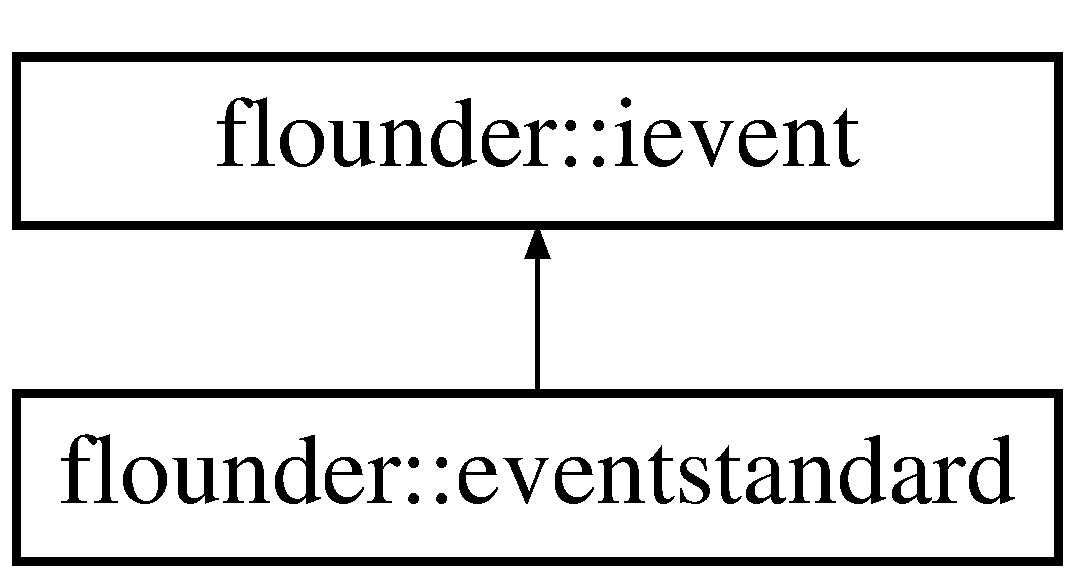
\includegraphics[height=2.000000cm]{classflounder_1_1eventstandard}
\end{center}
\end{figure}
\subsection*{Public Member Functions}
\begin{DoxyCompactItemize}
\item 
\hyperlink{classflounder_1_1eventstandard_a39d75790b90c11dee6a982f7ffeabebe}{eventstandard} (const bool \&repeat, const std\+::function$<$ bool()$>$ \&triggered, const std\+::function$<$ void()$>$ \&\hyperlink{classflounder_1_1eventstandard_af25e174b30e7d23698024b2c1ae9ac4c}{on\+Event})
\begin{DoxyCompactList}\small\item\em Creates a new standard event. \end{DoxyCompactList}\item 
\hyperlink{classflounder_1_1eventstandard_a63cfd71a0d3b80a18656673a651853a9}{eventstandard} (const std\+::function$<$ bool()$>$ \&triggered, const std\+::function$<$ void()$>$ \&\hyperlink{classflounder_1_1eventstandard_af25e174b30e7d23698024b2c1ae9ac4c}{on\+Event})
\begin{DoxyCompactList}\small\item\em Creates a new standard event that repeats. \end{DoxyCompactList}\item 
bool \hyperlink{classflounder_1_1eventstandard_a88224b7246627df26a08ec9e286e7496}{event\+Triggered} () override
\begin{DoxyCompactList}\small\item\em Gets if the event has occurred. \end{DoxyCompactList}\item 
void \hyperlink{classflounder_1_1eventstandard_af25e174b30e7d23698024b2c1ae9ac4c}{on\+Event} () override
\begin{DoxyCompactList}\small\item\em Run when a event has occurred. \end{DoxyCompactList}\item 
bool \hyperlink{classflounder_1_1eventstandard_ac4b9d57605f7f81c7c7e1cb981002f2f}{remove\+After\+Event} () override
\begin{DoxyCompactList}\small\item\em Gets if the event is removed after it has run once. \end{DoxyCompactList}\end{DoxyCompactItemize}
\subsection*{Private Attributes}
\begin{DoxyCompactItemize}
\item 
\mbox{\Hypertarget{classflounder_1_1eventstandard_a32fe9df9224d30665a3052d4f84dfc7d}\label{classflounder_1_1eventstandard_a32fe9df9224d30665a3052d4f84dfc7d}} 
bool {\bfseries m\+\_\+repeat}
\item 
\mbox{\Hypertarget{classflounder_1_1eventstandard_a5cfe152a10b4bb997e0f95b22ba7fc9e}\label{classflounder_1_1eventstandard_a5cfe152a10b4bb997e0f95b22ba7fc9e}} 
std\+::function$<$ bool()$>$ {\bfseries m\+\_\+triggered}
\item 
\mbox{\Hypertarget{classflounder_1_1eventstandard_a9d5030d3ce4419af226b1330c3b771c5}\label{classflounder_1_1eventstandard_a9d5030d3ce4419af226b1330c3b771c5}} 
std\+::function$<$ void()$>$ {\bfseries m\+\_\+on\+Event}
\end{DoxyCompactItemize}


\subsection{Detailed Description}
A class that is the most basic implementation of the event interface. 



\subsection{Constructor \& Destructor Documentation}
\mbox{\Hypertarget{classflounder_1_1eventstandard_a39d75790b90c11dee6a982f7ffeabebe}\label{classflounder_1_1eventstandard_a39d75790b90c11dee6a982f7ffeabebe}} 
\index{flounder\+::eventstandard@{flounder\+::eventstandard}!eventstandard@{eventstandard}}
\index{eventstandard@{eventstandard}!flounder\+::eventstandard@{flounder\+::eventstandard}}
\subsubsection{\texorpdfstring{eventstandard()}{eventstandard()}\hspace{0.1cm}{\footnotesize\ttfamily [1/2]}}
{\footnotesize\ttfamily flounder\+::eventstandard\+::eventstandard (\begin{DoxyParamCaption}\item[{const bool \&}]{repeat,  }\item[{const std\+::function$<$ bool()$>$ \&}]{triggered,  }\item[{const std\+::function$<$ void()$>$ \&}]{on\+Event }\end{DoxyParamCaption})}



Creates a new standard event. 


\begin{DoxyParams}{Parameters}
{\em repeat} & If the event will repeat after the first run. \\
\hline
{\em triggered} & A function called to check if the event was triggered. \\
\hline
{\em on\+Event} & A function called when the event is triggered. \\
\hline
\end{DoxyParams}
\mbox{\Hypertarget{classflounder_1_1eventstandard_a63cfd71a0d3b80a18656673a651853a9}\label{classflounder_1_1eventstandard_a63cfd71a0d3b80a18656673a651853a9}} 
\index{flounder\+::eventstandard@{flounder\+::eventstandard}!eventstandard@{eventstandard}}
\index{eventstandard@{eventstandard}!flounder\+::eventstandard@{flounder\+::eventstandard}}
\subsubsection{\texorpdfstring{eventstandard()}{eventstandard()}\hspace{0.1cm}{\footnotesize\ttfamily [2/2]}}
{\footnotesize\ttfamily flounder\+::eventstandard\+::eventstandard (\begin{DoxyParamCaption}\item[{const std\+::function$<$ bool()$>$ \&}]{triggered,  }\item[{const std\+::function$<$ void()$>$ \&}]{on\+Event }\end{DoxyParamCaption})}



Creates a new standard event that repeats. 


\begin{DoxyParams}{Parameters}
{\em triggered} & A function called to check if the event was triggered. \\
\hline
{\em on\+Event} & A function called when the event is triggered. \\
\hline
\end{DoxyParams}


\subsection{Member Function Documentation}
\mbox{\Hypertarget{classflounder_1_1eventstandard_a88224b7246627df26a08ec9e286e7496}\label{classflounder_1_1eventstandard_a88224b7246627df26a08ec9e286e7496}} 
\index{flounder\+::eventstandard@{flounder\+::eventstandard}!event\+Triggered@{event\+Triggered}}
\index{event\+Triggered@{event\+Triggered}!flounder\+::eventstandard@{flounder\+::eventstandard}}
\subsubsection{\texorpdfstring{event\+Triggered()}{eventTriggered()}}
{\footnotesize\ttfamily bool flounder\+::eventstandard\+::event\+Triggered (\begin{DoxyParamCaption}{ }\end{DoxyParamCaption})\hspace{0.3cm}{\ttfamily [override]}, {\ttfamily [virtual]}}



Gets if the event has occurred. 

\begin{DoxyReturn}{Returns}
The event has occurred. 
\end{DoxyReturn}


Implements \hyperlink{classflounder_1_1ievent_a4462f66feef99ef4e3521c00f4edd0c9}{flounder\+::ievent}.

\mbox{\Hypertarget{classflounder_1_1eventstandard_af25e174b30e7d23698024b2c1ae9ac4c}\label{classflounder_1_1eventstandard_af25e174b30e7d23698024b2c1ae9ac4c}} 
\index{flounder\+::eventstandard@{flounder\+::eventstandard}!on\+Event@{on\+Event}}
\index{on\+Event@{on\+Event}!flounder\+::eventstandard@{flounder\+::eventstandard}}
\subsubsection{\texorpdfstring{on\+Event()}{onEvent()}}
{\footnotesize\ttfamily void flounder\+::eventstandard\+::on\+Event (\begin{DoxyParamCaption}{ }\end{DoxyParamCaption})\hspace{0.3cm}{\ttfamily [override]}, {\ttfamily [virtual]}}



Run when a event has occurred. 



Implements \hyperlink{classflounder_1_1ievent_a6c6abe67435870b25eccd57a251a8992}{flounder\+::ievent}.

\mbox{\Hypertarget{classflounder_1_1eventstandard_ac4b9d57605f7f81c7c7e1cb981002f2f}\label{classflounder_1_1eventstandard_ac4b9d57605f7f81c7c7e1cb981002f2f}} 
\index{flounder\+::eventstandard@{flounder\+::eventstandard}!remove\+After\+Event@{remove\+After\+Event}}
\index{remove\+After\+Event@{remove\+After\+Event}!flounder\+::eventstandard@{flounder\+::eventstandard}}
\subsubsection{\texorpdfstring{remove\+After\+Event()}{removeAfterEvent()}}
{\footnotesize\ttfamily bool flounder\+::eventstandard\+::remove\+After\+Event (\begin{DoxyParamCaption}{ }\end{DoxyParamCaption})\hspace{0.3cm}{\ttfamily [inline]}, {\ttfamily [override]}, {\ttfamily [virtual]}}



Gets if the event is removed after it has run once. 

\begin{DoxyReturn}{Returns}
If the even will run. 
\end{DoxyReturn}


Implements \hyperlink{classflounder_1_1ievent_a7017c8803df2397758980cb61020e801}{flounder\+::ievent}.



The documentation for this class was generated from the following files\+:\begin{DoxyCompactItemize}
\item 
Flounder-\/\+Core/src/events/eventstandard.\+h\item 
Flounder-\/\+Core/src/events/eventstandard.\+cpp\end{DoxyCompactItemize}

\hypertarget{classflounder_1_1eventtime}{}\section{flounder\+:\+:eventtime Class Reference}
\label{classflounder_1_1eventtime}\index{flounder\+::eventtime@{flounder\+::eventtime}}


A class that runs a event after a time has passed.  




{\ttfamily \#include $<$eventtime.\+h$>$}

Inheritance diagram for flounder\+:\+:eventtime\+:\begin{figure}[H]
\begin{center}
\leavevmode
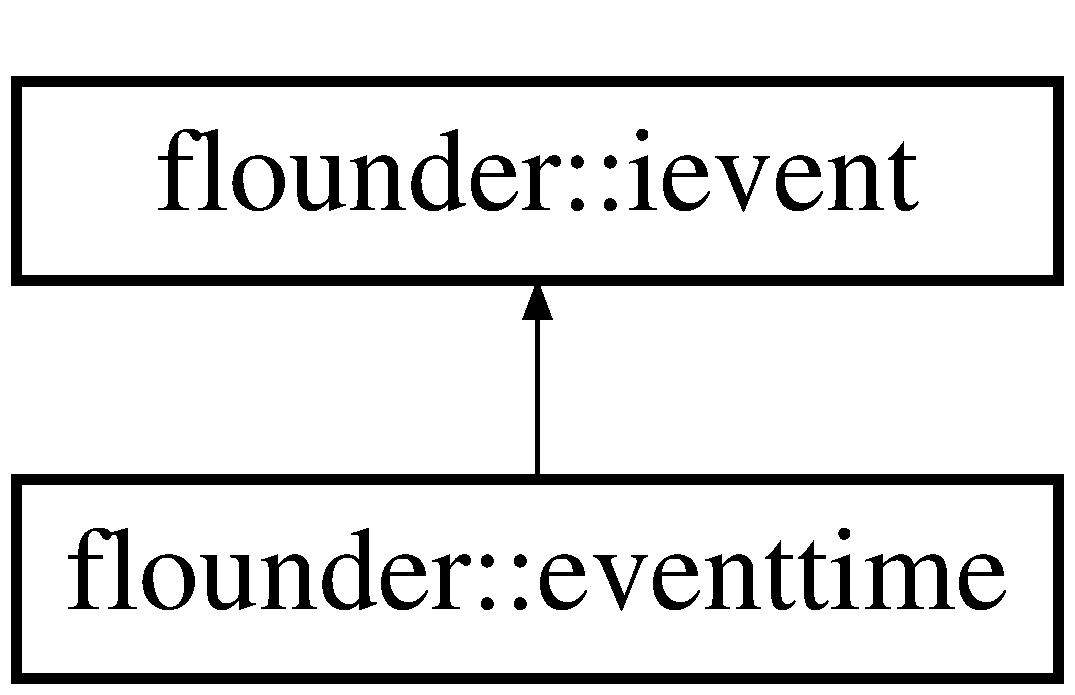
\includegraphics[height=2.000000cm]{classflounder_1_1eventtime}
\end{center}
\end{figure}
\subsection*{Public Member Functions}
\begin{DoxyCompactItemize}
\item 
\hyperlink{classflounder_1_1eventtime_a20972724acf2b8b681a1754d59adeff3}{eventtime} (const float \&interval, const bool \&repeat, const std\+::function$<$ void()$>$ \&\hyperlink{classflounder_1_1eventtime_a1b066c00fa959786bb1e9bbd1d212691}{on\+Event})
\begin{DoxyCompactList}\small\item\em Creates a new time event. \end{DoxyCompactList}\item 
\hyperlink{classflounder_1_1eventtime_a30e85c8870687c7b8fabaf6496381366}{$\sim$eventtime} ()
\begin{DoxyCompactList}\small\item\em Deconstructor for the timed event. \end{DoxyCompactList}\item 
bool \hyperlink{classflounder_1_1eventtime_a67a616128c8e4701f7e229172c5e80a5}{event\+Triggered} () override
\begin{DoxyCompactList}\small\item\em Gets if the event has occurred. \end{DoxyCompactList}\item 
void \hyperlink{classflounder_1_1eventtime_a1b066c00fa959786bb1e9bbd1d212691}{on\+Event} () override
\begin{DoxyCompactList}\small\item\em Run when a event has occurred. \end{DoxyCompactList}\item 
bool \hyperlink{classflounder_1_1eventtime_ad765cd1e3b8fe2bf95f2290f5c625af1}{remove\+After\+Event} () override
\begin{DoxyCompactList}\small\item\em Gets if the event is removed after it has run once. \end{DoxyCompactList}\end{DoxyCompactItemize}
\subsection*{Private Attributes}
\begin{DoxyCompactItemize}
\item 
\mbox{\Hypertarget{classflounder_1_1eventtime_a955a7db17c2f5011797a34fda333d2dc}\label{classflounder_1_1eventtime_a955a7db17c2f5011797a34fda333d2dc}} 
\hyperlink{classflounder_1_1timer}{timer} $\ast$ {\bfseries m\+\_\+timer}
\item 
\mbox{\Hypertarget{classflounder_1_1eventtime_abf987190be93e422cd53a8e5dac07218}\label{classflounder_1_1eventtime_abf987190be93e422cd53a8e5dac07218}} 
bool {\bfseries m\+\_\+repeat}
\item 
\mbox{\Hypertarget{classflounder_1_1eventtime_af793eee748651cb6d9a568b1845e4f4a}\label{classflounder_1_1eventtime_af793eee748651cb6d9a568b1845e4f4a}} 
std\+::function$<$ void()$>$ {\bfseries m\+\_\+on\+Event}
\end{DoxyCompactItemize}


\subsection{Detailed Description}
A class that runs a event after a time has passed. 



\subsection{Constructor \& Destructor Documentation}
\mbox{\Hypertarget{classflounder_1_1eventtime_a20972724acf2b8b681a1754d59adeff3}\label{classflounder_1_1eventtime_a20972724acf2b8b681a1754d59adeff3}} 
\index{flounder\+::eventtime@{flounder\+::eventtime}!eventtime@{eventtime}}
\index{eventtime@{eventtime}!flounder\+::eventtime@{flounder\+::eventtime}}
\subsubsection{\texorpdfstring{eventtime()}{eventtime()}}
{\footnotesize\ttfamily flounder\+::eventtime\+::eventtime (\begin{DoxyParamCaption}\item[{const float \&}]{interval,  }\item[{const bool \&}]{repeat,  }\item[{const std\+::function$<$ void()$>$ \&}]{on\+Event }\end{DoxyParamCaption})}



Creates a new time event. 


\begin{DoxyParams}{Parameters}
{\em interval} & The amount of seconds in the future to run the event. \\
\hline
{\em repeat} & If the event will repeat after the first run. \\
\hline
{\em on\+Event} & A function called when the event is triggered. \\
\hline
\end{DoxyParams}
\mbox{\Hypertarget{classflounder_1_1eventtime_a30e85c8870687c7b8fabaf6496381366}\label{classflounder_1_1eventtime_a30e85c8870687c7b8fabaf6496381366}} 
\index{flounder\+::eventtime@{flounder\+::eventtime}!````~eventtime@{$\sim$eventtime}}
\index{````~eventtime@{$\sim$eventtime}!flounder\+::eventtime@{flounder\+::eventtime}}
\subsubsection{\texorpdfstring{$\sim$eventtime()}{~eventtime()}}
{\footnotesize\ttfamily flounder\+::eventtime\+::$\sim$eventtime (\begin{DoxyParamCaption}{ }\end{DoxyParamCaption})}



Deconstructor for the timed event. 



\subsection{Member Function Documentation}
\mbox{\Hypertarget{classflounder_1_1eventtime_a67a616128c8e4701f7e229172c5e80a5}\label{classflounder_1_1eventtime_a67a616128c8e4701f7e229172c5e80a5}} 
\index{flounder\+::eventtime@{flounder\+::eventtime}!event\+Triggered@{event\+Triggered}}
\index{event\+Triggered@{event\+Triggered}!flounder\+::eventtime@{flounder\+::eventtime}}
\subsubsection{\texorpdfstring{event\+Triggered()}{eventTriggered()}}
{\footnotesize\ttfamily bool flounder\+::eventtime\+::event\+Triggered (\begin{DoxyParamCaption}{ }\end{DoxyParamCaption})\hspace{0.3cm}{\ttfamily [override]}, {\ttfamily [virtual]}}



Gets if the event has occurred. 

\begin{DoxyReturn}{Returns}
The event has occurred. 
\end{DoxyReturn}


Implements \hyperlink{classflounder_1_1ievent_a4462f66feef99ef4e3521c00f4edd0c9}{flounder\+::ievent}.

\mbox{\Hypertarget{classflounder_1_1eventtime_a1b066c00fa959786bb1e9bbd1d212691}\label{classflounder_1_1eventtime_a1b066c00fa959786bb1e9bbd1d212691}} 
\index{flounder\+::eventtime@{flounder\+::eventtime}!on\+Event@{on\+Event}}
\index{on\+Event@{on\+Event}!flounder\+::eventtime@{flounder\+::eventtime}}
\subsubsection{\texorpdfstring{on\+Event()}{onEvent()}}
{\footnotesize\ttfamily void flounder\+::eventtime\+::on\+Event (\begin{DoxyParamCaption}{ }\end{DoxyParamCaption})\hspace{0.3cm}{\ttfamily [override]}, {\ttfamily [virtual]}}



Run when a event has occurred. 



Implements \hyperlink{classflounder_1_1ievent_a6c6abe67435870b25eccd57a251a8992}{flounder\+::ievent}.

\mbox{\Hypertarget{classflounder_1_1eventtime_ad765cd1e3b8fe2bf95f2290f5c625af1}\label{classflounder_1_1eventtime_ad765cd1e3b8fe2bf95f2290f5c625af1}} 
\index{flounder\+::eventtime@{flounder\+::eventtime}!remove\+After\+Event@{remove\+After\+Event}}
\index{remove\+After\+Event@{remove\+After\+Event}!flounder\+::eventtime@{flounder\+::eventtime}}
\subsubsection{\texorpdfstring{remove\+After\+Event()}{removeAfterEvent()}}
{\footnotesize\ttfamily bool flounder\+::eventtime\+::remove\+After\+Event (\begin{DoxyParamCaption}{ }\end{DoxyParamCaption})\hspace{0.3cm}{\ttfamily [inline]}, {\ttfamily [override]}, {\ttfamily [virtual]}}



Gets if the event is removed after it has run once. 

\begin{DoxyReturn}{Returns}
If the even will run. 
\end{DoxyReturn}


Implements \hyperlink{classflounder_1_1ievent_a7017c8803df2397758980cb61020e801}{flounder\+::ievent}.



The documentation for this class was generated from the following files\+:\begin{DoxyCompactItemize}
\item 
Flounder-\/\+Core/src/events/eventtime.\+h\item 
Flounder-\/\+Core/src/events/eventtime.\+cpp\end{DoxyCompactItemize}

\hypertarget{classflounder_1_1filterbloom1}{}\section{flounder\+:\+:filterbloom1 Class Reference}
\label{classflounder_1_1filterbloom1}\index{flounder\+::filterbloom1@{flounder\+::filterbloom1}}
Inheritance diagram for flounder\+:\+:filterbloom1\+:\begin{figure}[H]
\begin{center}
\leavevmode
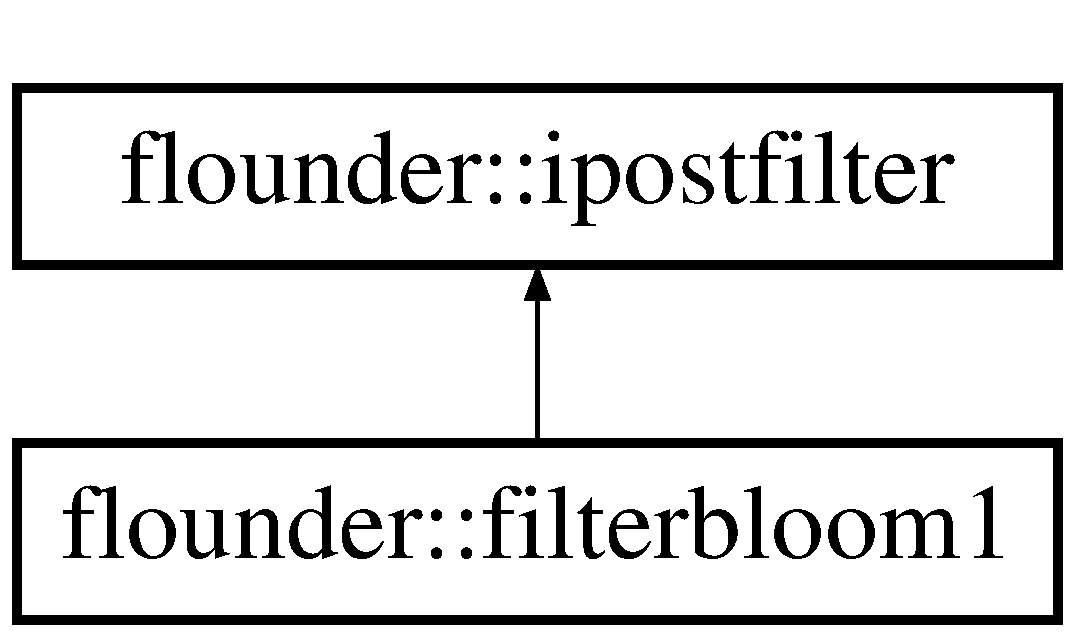
\includegraphics[height=2.000000cm]{classflounder_1_1filterbloom1}
\end{center}
\end{figure}
\subsection*{Public Member Functions}
\begin{DoxyCompactItemize}
\item 
void \hyperlink{classflounder_1_1filterbloom1_adfa3f732b13f449745418bf9bd539f79}{store\+Values} () override
\begin{DoxyCompactList}\small\item\em Can be used to store values into the shader, this is called when the filter is applied and the shader has been already started. \end{DoxyCompactList}\end{DoxyCompactItemize}
\subsection*{Additional Inherited Members}


\subsection{Member Function Documentation}
\mbox{\Hypertarget{classflounder_1_1filterbloom1_adfa3f732b13f449745418bf9bd539f79}\label{classflounder_1_1filterbloom1_adfa3f732b13f449745418bf9bd539f79}} 
\index{flounder\+::filterbloom1@{flounder\+::filterbloom1}!store\+Values@{store\+Values}}
\index{store\+Values@{store\+Values}!flounder\+::filterbloom1@{flounder\+::filterbloom1}}
\subsubsection{\texorpdfstring{store\+Values()}{storeValues()}}
{\footnotesize\ttfamily void flounder\+::filterbloom1\+::store\+Values (\begin{DoxyParamCaption}{ }\end{DoxyParamCaption})\hspace{0.3cm}{\ttfamily [override]}, {\ttfamily [virtual]}}



Can be used to store values into the shader, this is called when the filter is applied and the shader has been already started. 



Implements \hyperlink{classflounder_1_1ipostfilter_a9b658b4672718d5ac36539875bde722e}{flounder\+::ipostfilter}.



The documentation for this class was generated from the following files\+:\begin{DoxyCompactItemize}
\item 
Flounder-\/\+Core/src/post/filters/filterbloom1.\+h\item 
Flounder-\/\+Core/src/post/filters/filterbloom1.\+cpp\end{DoxyCompactItemize}

\hypertarget{classflounder_1_1filterbloom2}{}\section{flounder\+:\+:filterbloom2 Class Reference}
\label{classflounder_1_1filterbloom2}\index{flounder\+::filterbloom2@{flounder\+::filterbloom2}}
Inheritance diagram for flounder\+:\+:filterbloom2\+:\begin{figure}[H]
\begin{center}
\leavevmode
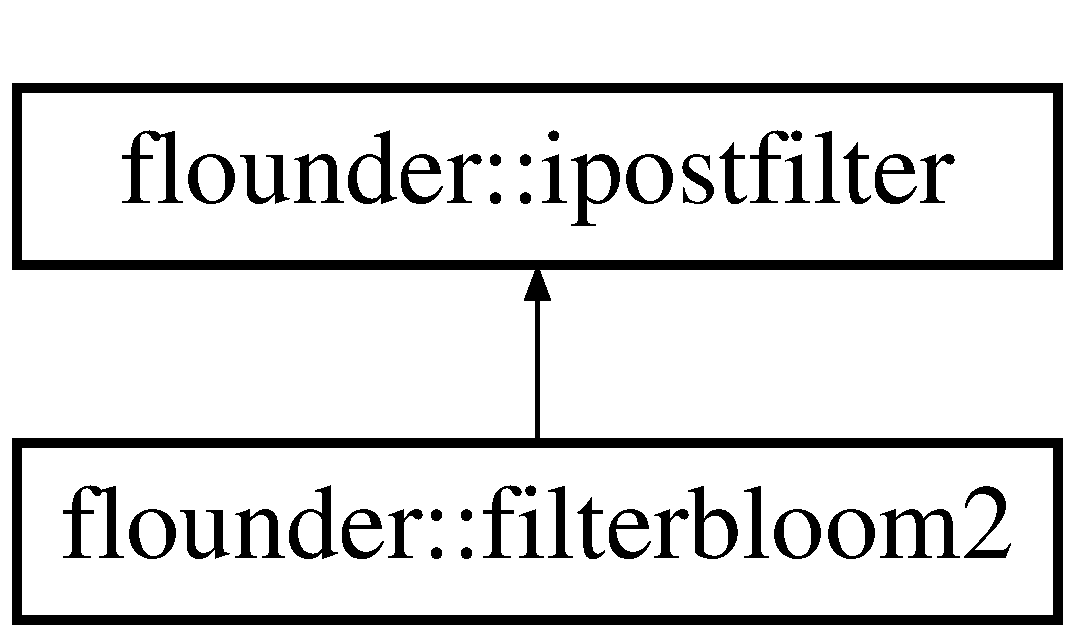
\includegraphics[height=2.000000cm]{classflounder_1_1filterbloom2}
\end{center}
\end{figure}
\subsection*{Public Member Functions}
\begin{DoxyCompactItemize}
\item 
void \hyperlink{classflounder_1_1filterbloom2_a6439fc5d762213a5f780033d6b88428e}{store\+Values} () override
\begin{DoxyCompactList}\small\item\em Can be used to store values into the shader, this is called when the filter is applied and the shader has been already started. \end{DoxyCompactList}\end{DoxyCompactItemize}
\subsection*{Additional Inherited Members}


\subsection{Member Function Documentation}
\mbox{\Hypertarget{classflounder_1_1filterbloom2_a6439fc5d762213a5f780033d6b88428e}\label{classflounder_1_1filterbloom2_a6439fc5d762213a5f780033d6b88428e}} 
\index{flounder\+::filterbloom2@{flounder\+::filterbloom2}!store\+Values@{store\+Values}}
\index{store\+Values@{store\+Values}!flounder\+::filterbloom2@{flounder\+::filterbloom2}}
\subsubsection{\texorpdfstring{store\+Values()}{storeValues()}}
{\footnotesize\ttfamily void flounder\+::filterbloom2\+::store\+Values (\begin{DoxyParamCaption}{ }\end{DoxyParamCaption})\hspace{0.3cm}{\ttfamily [override]}, {\ttfamily [virtual]}}



Can be used to store values into the shader, this is called when the filter is applied and the shader has been already started. 



Implements \hyperlink{classflounder_1_1ipostfilter_a9b658b4672718d5ac36539875bde722e}{flounder\+::ipostfilter}.



The documentation for this class was generated from the following files\+:\begin{DoxyCompactItemize}
\item 
Flounder-\/\+Core/src/post/filters/filterbloom2.\+h\item 
Flounder-\/\+Core/src/post/filters/filterbloom2.\+cpp\end{DoxyCompactItemize}

\hypertarget{classflounder_1_1filterblurhorizontal}{}\section{flounder\+:\+:filterblurhorizontal Class Reference}
\label{classflounder_1_1filterblurhorizontal}\index{flounder\+::filterblurhorizontal@{flounder\+::filterblurhorizontal}}
Inheritance diagram for flounder\+:\+:filterblurhorizontal\+:\begin{figure}[H]
\begin{center}
\leavevmode
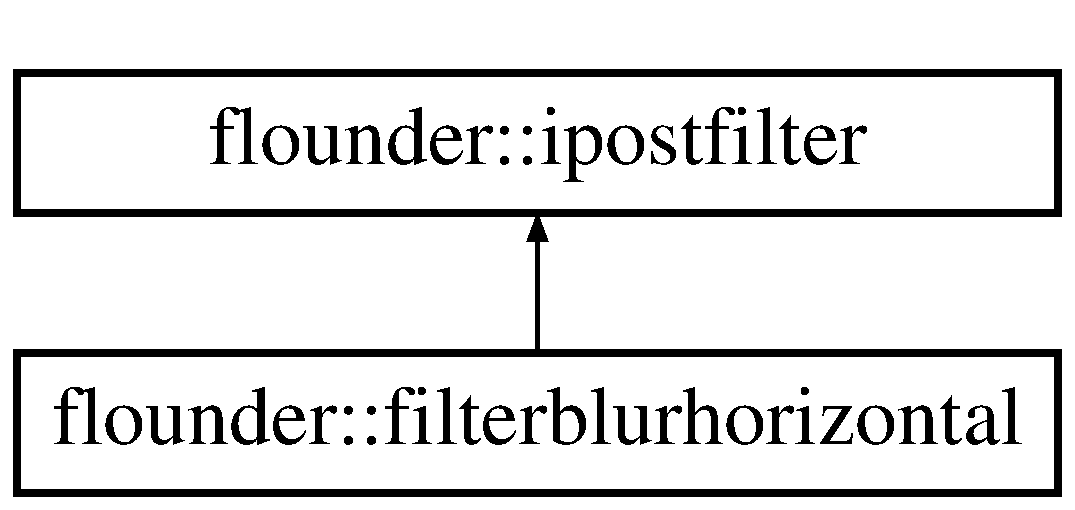
\includegraphics[height=2.000000cm]{classflounder_1_1filterblurhorizontal}
\end{center}
\end{figure}
\subsection*{Public Member Functions}
\begin{DoxyCompactItemize}
\item 
\mbox{\Hypertarget{classflounder_1_1filterblurhorizontal_a8a160123b253eb281ce9f8c73d37e95e}\label{classflounder_1_1filterblurhorizontal_a8a160123b253eb281ce9f8c73d37e95e}} 
{\bfseries filterblurhorizontal} (const float \&size\+Scalar)
\item 
\mbox{\Hypertarget{classflounder_1_1filterblurhorizontal_ad7f43ae378a048236bf715ba969cece3}\label{classflounder_1_1filterblurhorizontal_ad7f43ae378a048236bf715ba969cece3}} 
{\bfseries filterblurhorizontal} (const int \&width, const int \&height)
\item 
void \hyperlink{classflounder_1_1filterblurhorizontal_ad147fceebdebffd0731fc346370021f7}{store\+Values} () override
\begin{DoxyCompactList}\small\item\em Can be used to store values into the shader, this is called when the filter is applied and the shader has been already started. \end{DoxyCompactList}\item 
\mbox{\Hypertarget{classflounder_1_1filterblurhorizontal_a2b27fc8a35c15b1b858855c9cc5b9cbd}\label{classflounder_1_1filterblurhorizontal_a2b27fc8a35c15b1b858855c9cc5b9cbd}} 
void {\bfseries set\+Scale\+Value} (const float \&scale\+Value)
\end{DoxyCompactItemize}
\subsection*{Private Attributes}
\begin{DoxyCompactItemize}
\item 
\mbox{\Hypertarget{classflounder_1_1filterblurhorizontal_a7ad006e2db54c64f94123f1dc4918408}\label{classflounder_1_1filterblurhorizontal_a7ad006e2db54c64f94123f1dc4918408}} 
int {\bfseries m\+\_\+width\+Value}
\item 
\mbox{\Hypertarget{classflounder_1_1filterblurhorizontal_a26c12d3356891c151bf9aab649fcd887}\label{classflounder_1_1filterblurhorizontal_a26c12d3356891c151bf9aab649fcd887}} 
float {\bfseries m\+\_\+scale\+Value}
\item 
\mbox{\Hypertarget{classflounder_1_1filterblurhorizontal_ae867b04caea9cff2e91339c62c834e0a}\label{classflounder_1_1filterblurhorizontal_ae867b04caea9cff2e91339c62c834e0a}} 
bool {\bfseries m\+\_\+fit\+To\+Display}
\item 
\mbox{\Hypertarget{classflounder_1_1filterblurhorizontal_a9cc551f29e574003b393f0ad1eeb2b9d}\label{classflounder_1_1filterblurhorizontal_a9cc551f29e574003b393f0ad1eeb2b9d}} 
float {\bfseries m\+\_\+size\+Scalar}
\end{DoxyCompactItemize}
\subsection*{Additional Inherited Members}


\subsection{Member Function Documentation}
\mbox{\Hypertarget{classflounder_1_1filterblurhorizontal_ad147fceebdebffd0731fc346370021f7}\label{classflounder_1_1filterblurhorizontal_ad147fceebdebffd0731fc346370021f7}} 
\index{flounder\+::filterblurhorizontal@{flounder\+::filterblurhorizontal}!store\+Values@{store\+Values}}
\index{store\+Values@{store\+Values}!flounder\+::filterblurhorizontal@{flounder\+::filterblurhorizontal}}
\subsubsection{\texorpdfstring{store\+Values()}{storeValues()}}
{\footnotesize\ttfamily void flounder\+::filterblurhorizontal\+::store\+Values (\begin{DoxyParamCaption}{ }\end{DoxyParamCaption})\hspace{0.3cm}{\ttfamily [override]}, {\ttfamily [virtual]}}



Can be used to store values into the shader, this is called when the filter is applied and the shader has been already started. 



Implements \hyperlink{classflounder_1_1ipostfilter_a9b658b4672718d5ac36539875bde722e}{flounder\+::ipostfilter}.



The documentation for this class was generated from the following files\+:\begin{DoxyCompactItemize}
\item 
Flounder-\/\+Core/src/post/filters/filterblurhorizontal.\+h\item 
Flounder-\/\+Core/src/post/filters/filterblurhorizontal.\+cpp\end{DoxyCompactItemize}

\hypertarget{classflounder_1_1filterblurvertical}{}\section{flounder\+:\+:filterblurvertical Class Reference}
\label{classflounder_1_1filterblurvertical}\index{flounder\+::filterblurvertical@{flounder\+::filterblurvertical}}
Inheritance diagram for flounder\+:\+:filterblurvertical\+:\begin{figure}[H]
\begin{center}
\leavevmode
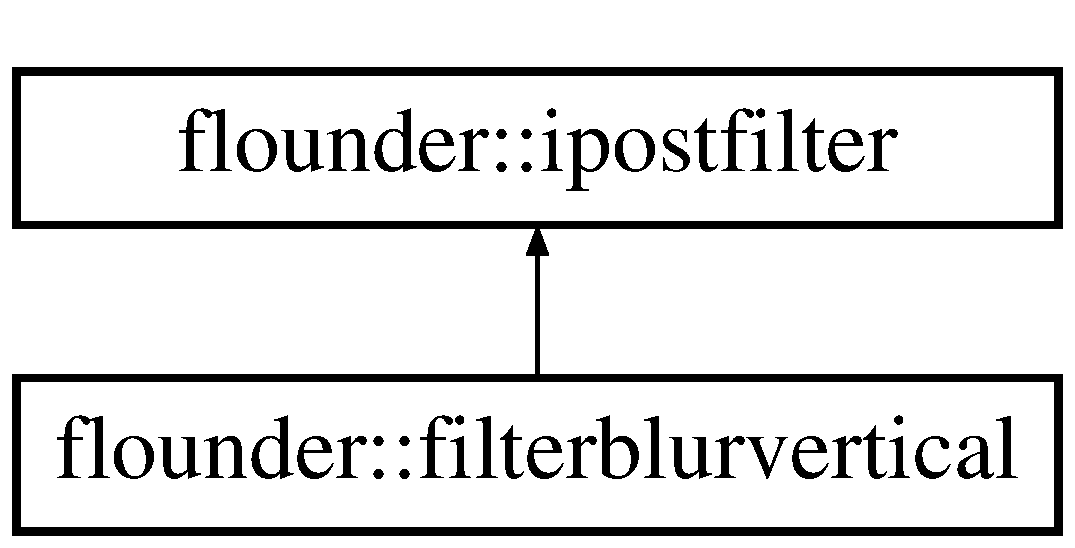
\includegraphics[height=2.000000cm]{classflounder_1_1filterblurvertical}
\end{center}
\end{figure}
\subsection*{Public Member Functions}
\begin{DoxyCompactItemize}
\item 
\mbox{\Hypertarget{classflounder_1_1filterblurvertical_a4762c1d32016cc81dfb67a001308f5a2}\label{classflounder_1_1filterblurvertical_a4762c1d32016cc81dfb67a001308f5a2}} 
{\bfseries filterblurvertical} (const float \&size\+Scalar)
\item 
\mbox{\Hypertarget{classflounder_1_1filterblurvertical_ad3399e213b743f1dbc44b1254363feb5}\label{classflounder_1_1filterblurvertical_ad3399e213b743f1dbc44b1254363feb5}} 
{\bfseries filterblurvertical} (const int \&width, const int \&height)
\item 
void \hyperlink{classflounder_1_1filterblurvertical_acdc191b6c9b067c9619055c1672dd2e5}{store\+Values} () override
\begin{DoxyCompactList}\small\item\em Can be used to store values into the shader, this is called when the filter is applied and the shader has been already started. \end{DoxyCompactList}\item 
\mbox{\Hypertarget{classflounder_1_1filterblurvertical_a4640c8ef21b48d8f8e853d8d92232d78}\label{classflounder_1_1filterblurvertical_a4640c8ef21b48d8f8e853d8d92232d78}} 
void {\bfseries set\+Scale\+Value} (const float \&scale\+Value)
\end{DoxyCompactItemize}
\subsection*{Private Attributes}
\begin{DoxyCompactItemize}
\item 
\mbox{\Hypertarget{classflounder_1_1filterblurvertical_ae12de62dab1a199092838d7d8401904a}\label{classflounder_1_1filterblurvertical_ae12de62dab1a199092838d7d8401904a}} 
int {\bfseries m\+\_\+height\+Value}
\item 
\mbox{\Hypertarget{classflounder_1_1filterblurvertical_a0fffea96668635a54361a32fe065848a}\label{classflounder_1_1filterblurvertical_a0fffea96668635a54361a32fe065848a}} 
float {\bfseries m\+\_\+scale\+Value}
\item 
\mbox{\Hypertarget{classflounder_1_1filterblurvertical_a9c94d85b9b6a6870f0202d95b1753850}\label{classflounder_1_1filterblurvertical_a9c94d85b9b6a6870f0202d95b1753850}} 
bool {\bfseries m\+\_\+fit\+To\+Display}
\item 
\mbox{\Hypertarget{classflounder_1_1filterblurvertical_a03c3471d445c686e901bf519fbe6e414}\label{classflounder_1_1filterblurvertical_a03c3471d445c686e901bf519fbe6e414}} 
float {\bfseries m\+\_\+size\+Scalar}
\end{DoxyCompactItemize}
\subsection*{Additional Inherited Members}


\subsection{Member Function Documentation}
\mbox{\Hypertarget{classflounder_1_1filterblurvertical_acdc191b6c9b067c9619055c1672dd2e5}\label{classflounder_1_1filterblurvertical_acdc191b6c9b067c9619055c1672dd2e5}} 
\index{flounder\+::filterblurvertical@{flounder\+::filterblurvertical}!store\+Values@{store\+Values}}
\index{store\+Values@{store\+Values}!flounder\+::filterblurvertical@{flounder\+::filterblurvertical}}
\subsubsection{\texorpdfstring{store\+Values()}{storeValues()}}
{\footnotesize\ttfamily void flounder\+::filterblurvertical\+::store\+Values (\begin{DoxyParamCaption}{ }\end{DoxyParamCaption})\hspace{0.3cm}{\ttfamily [override]}, {\ttfamily [virtual]}}



Can be used to store values into the shader, this is called when the filter is applied and the shader has been already started. 



Implements \hyperlink{classflounder_1_1ipostfilter_a9b658b4672718d5ac36539875bde722e}{flounder\+::ipostfilter}.



The documentation for this class was generated from the following files\+:\begin{DoxyCompactItemize}
\item 
Flounder-\/\+Core/src/post/filters/filterblurvertical.\+h\item 
Flounder-\/\+Core/src/post/filters/filterblurvertical.\+cpp\end{DoxyCompactItemize}

\hypertarget{classflounder_1_1filtercombine}{}\section{flounder\+:\+:filtercombine Class Reference}
\label{classflounder_1_1filtercombine}\index{flounder\+::filtercombine@{flounder\+::filtercombine}}
Inheritance diagram for flounder\+:\+:filtercombine\+:\begin{figure}[H]
\begin{center}
\leavevmode
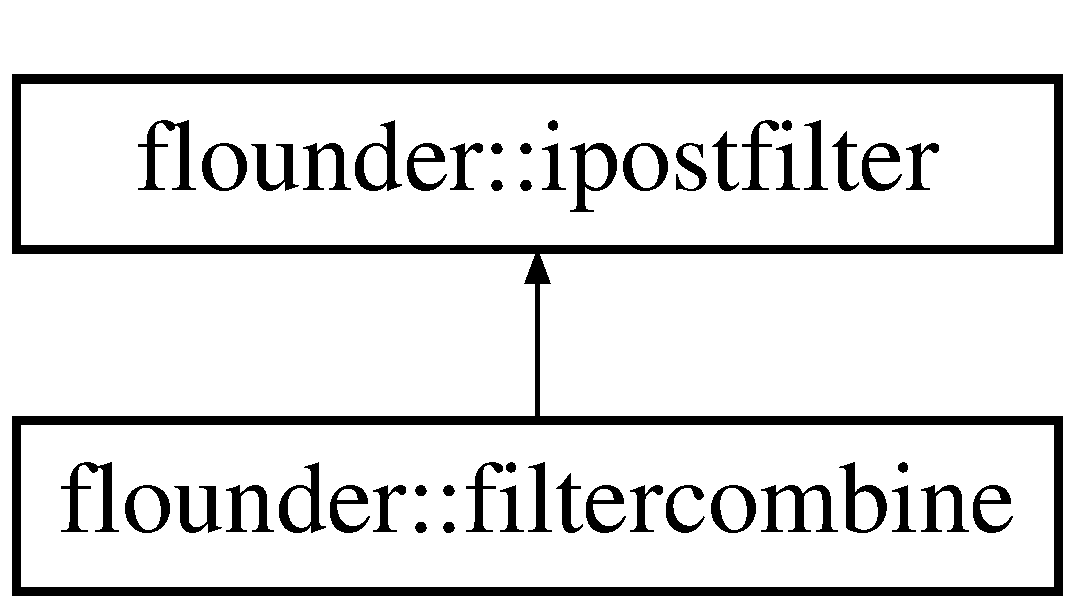
\includegraphics[height=2.000000cm]{classflounder_1_1filtercombine}
\end{center}
\end{figure}
\subsection*{Public Member Functions}
\begin{DoxyCompactItemize}
\item 
void \hyperlink{classflounder_1_1filtercombine_a0ec0634422d3ed539045d9fcfa3d119e}{store\+Values} () override
\begin{DoxyCompactList}\small\item\em Can be used to store values into the shader, this is called when the filter is applied and the shader has been already started. \end{DoxyCompactList}\item 
\mbox{\Hypertarget{classflounder_1_1filtercombine_acc8abe49dfbe2c04ffae152e3fc5306f}\label{classflounder_1_1filtercombine_acc8abe49dfbe2c04ffae152e3fc5306f}} 
void {\bfseries set\+Slide\+Space\+Value} (const \hyperlink{classflounder_1_1vector4}{vector4} \&slide\+Space\+Value)
\item 
\mbox{\Hypertarget{classflounder_1_1filtercombine_a14cb86373ccc0ba66bc6ce485806589d}\label{classflounder_1_1filtercombine_a14cb86373ccc0ba66bc6ce485806589d}} 
void {\bfseries set\+Slide\+Space} (const float \&x, const float \&y, const float \&z, const float \&w)
\end{DoxyCompactItemize}
\subsection*{Private Attributes}
\begin{DoxyCompactItemize}
\item 
\mbox{\Hypertarget{classflounder_1_1filtercombine_a54359b6adfe0a65305325202de649bfe}\label{classflounder_1_1filtercombine_a54359b6adfe0a65305325202de649bfe}} 
\hyperlink{classflounder_1_1vector4}{vector4} $\ast$ {\bfseries m\+\_\+slide\+Space\+Value}
\end{DoxyCompactItemize}
\subsection*{Additional Inherited Members}


\subsection{Member Function Documentation}
\mbox{\Hypertarget{classflounder_1_1filtercombine_a0ec0634422d3ed539045d9fcfa3d119e}\label{classflounder_1_1filtercombine_a0ec0634422d3ed539045d9fcfa3d119e}} 
\index{flounder\+::filtercombine@{flounder\+::filtercombine}!store\+Values@{store\+Values}}
\index{store\+Values@{store\+Values}!flounder\+::filtercombine@{flounder\+::filtercombine}}
\subsubsection{\texorpdfstring{store\+Values()}{storeValues()}}
{\footnotesize\ttfamily void flounder\+::filtercombine\+::store\+Values (\begin{DoxyParamCaption}{ }\end{DoxyParamCaption})\hspace{0.3cm}{\ttfamily [override]}, {\ttfamily [virtual]}}



Can be used to store values into the shader, this is called when the filter is applied and the shader has been already started. 



Implements \hyperlink{classflounder_1_1ipostfilter_a9b658b4672718d5ac36539875bde722e}{flounder\+::ipostfilter}.



The documentation for this class was generated from the following files\+:\begin{DoxyCompactItemize}
\item 
Flounder-\/\+Core/src/post/filters/filtercombine.\+h\item 
Flounder-\/\+Core/src/post/filters/filtercombine.\+cpp\end{DoxyCompactItemize}

\hypertarget{classflounder_1_1filtercrt}{}\section{flounder\+:\+:filtercrt Class Reference}
\label{classflounder_1_1filtercrt}\index{flounder\+::filtercrt@{flounder\+::filtercrt}}
Inheritance diagram for flounder\+:\+:filtercrt\+:\begin{figure}[H]
\begin{center}
\leavevmode
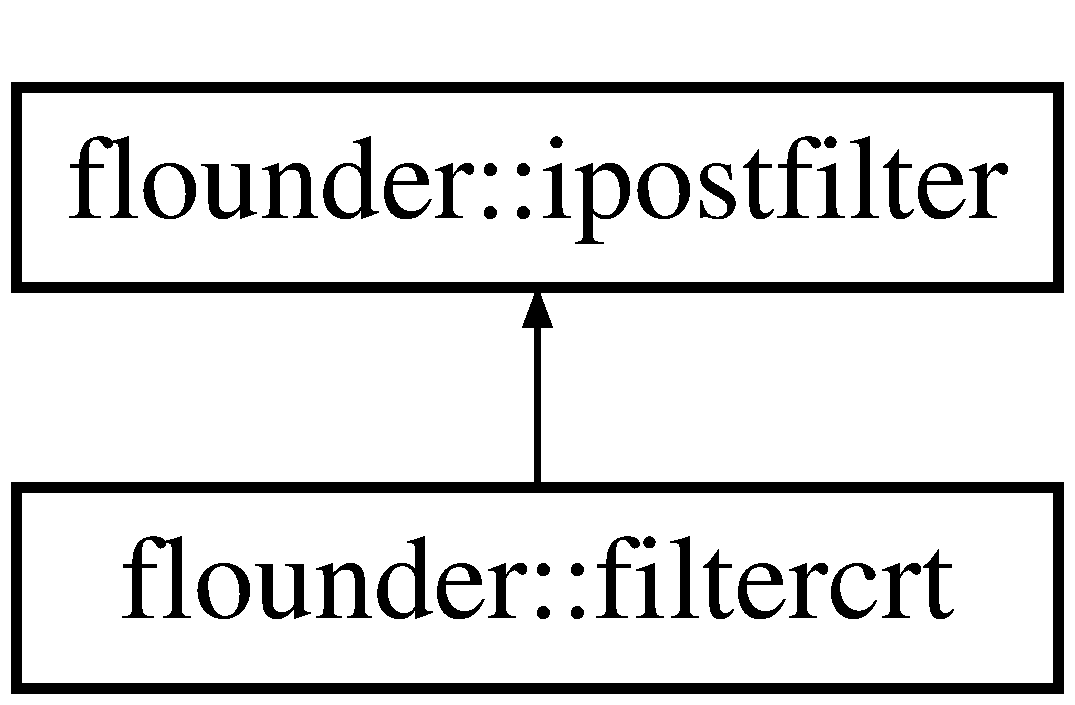
\includegraphics[height=2.000000cm]{classflounder_1_1filtercrt}
\end{center}
\end{figure}
\subsection*{Public Member Functions}
\begin{DoxyCompactItemize}
\item 
\mbox{\Hypertarget{classflounder_1_1filtercrt_aeceb7db9c18f0e13242fa1895b142e59}\label{classflounder_1_1filtercrt_aeceb7db9c18f0e13242fa1895b142e59}} 
{\bfseries filtercrt} (\hyperlink{classflounder_1_1colour}{colour} $\ast$screen\+Colour, const float \&curve\+AmountX, const float \&curve\+AmountY, const float \&scan\+Line\+Size, const float \&scan\+Intensity)
\item 
void \hyperlink{classflounder_1_1filtercrt_a6b3d151d6e338a7c859aeea1016724dc}{store\+Values} () override
\begin{DoxyCompactList}\small\item\em Can be used to store values into the shader, this is called when the filter is applied and the shader has been already started. \end{DoxyCompactList}\item 
\mbox{\Hypertarget{classflounder_1_1filtercrt_ac156aff36d490b409b1911f2893bd95f}\label{classflounder_1_1filtercrt_ac156aff36d490b409b1911f2893bd95f}} 
void {\bfseries set\+Screen\+Colour} (const \hyperlink{classflounder_1_1colour}{colour} \&screen\+Colour)
\item 
\mbox{\Hypertarget{classflounder_1_1filtercrt_a74e9525a871edaeb291a3470b5c58dd3}\label{classflounder_1_1filtercrt_a74e9525a871edaeb291a3470b5c58dd3}} 
void {\bfseries set\+Curve\+AmountX} (const float \&curve\+AmountX)
\item 
\mbox{\Hypertarget{classflounder_1_1filtercrt_af240aa2427e6b14021fa60780788822f}\label{classflounder_1_1filtercrt_af240aa2427e6b14021fa60780788822f}} 
void {\bfseries set\+Curve\+AmountY} (const float \&curve\+AmountY)
\item 
\mbox{\Hypertarget{classflounder_1_1filtercrt_af05d18c6418e6adfe6a798f3f86d171a}\label{classflounder_1_1filtercrt_af05d18c6418e6adfe6a798f3f86d171a}} 
void {\bfseries set\+Scan\+Line\+Size} (const float \&scan\+Line\+Size)
\item 
\mbox{\Hypertarget{classflounder_1_1filtercrt_ac4b470e46a16c4625ade473ac00ac758}\label{classflounder_1_1filtercrt_ac4b470e46a16c4625ade473ac00ac758}} 
void {\bfseries set\+Scan\+Intensity} (const float \&scan\+Intensity)
\end{DoxyCompactItemize}
\subsection*{Private Attributes}
\begin{DoxyCompactItemize}
\item 
\mbox{\Hypertarget{classflounder_1_1filtercrt_a748eeea34c823085a53c1d0631d0104b}\label{classflounder_1_1filtercrt_a748eeea34c823085a53c1d0631d0104b}} 
\hyperlink{classflounder_1_1colour}{colour} $\ast$ {\bfseries m\+\_\+screen\+Colour}
\item 
\mbox{\Hypertarget{classflounder_1_1filtercrt_a8edb88d85bdfb4b7dca89366460e721b}\label{classflounder_1_1filtercrt_a8edb88d85bdfb4b7dca89366460e721b}} 
float {\bfseries m\+\_\+curve\+AmountX}
\item 
\mbox{\Hypertarget{classflounder_1_1filtercrt_ac1210ea97957231c933ac86a95764400}\label{classflounder_1_1filtercrt_ac1210ea97957231c933ac86a95764400}} 
float {\bfseries m\+\_\+curve\+AmountY}
\item 
\mbox{\Hypertarget{classflounder_1_1filtercrt_a3b90d6d75537b4e6b4e492dfb18f7cf8}\label{classflounder_1_1filtercrt_a3b90d6d75537b4e6b4e492dfb18f7cf8}} 
float {\bfseries m\+\_\+scan\+Line\+Size}
\item 
\mbox{\Hypertarget{classflounder_1_1filtercrt_a8dc28e43a32d9430c57225c9bd1a063d}\label{classflounder_1_1filtercrt_a8dc28e43a32d9430c57225c9bd1a063d}} 
float {\bfseries m\+\_\+scan\+Intensity}
\end{DoxyCompactItemize}
\subsection*{Additional Inherited Members}


\subsection{Member Function Documentation}
\mbox{\Hypertarget{classflounder_1_1filtercrt_a6b3d151d6e338a7c859aeea1016724dc}\label{classflounder_1_1filtercrt_a6b3d151d6e338a7c859aeea1016724dc}} 
\index{flounder\+::filtercrt@{flounder\+::filtercrt}!store\+Values@{store\+Values}}
\index{store\+Values@{store\+Values}!flounder\+::filtercrt@{flounder\+::filtercrt}}
\subsubsection{\texorpdfstring{store\+Values()}{storeValues()}}
{\footnotesize\ttfamily void flounder\+::filtercrt\+::store\+Values (\begin{DoxyParamCaption}{ }\end{DoxyParamCaption})\hspace{0.3cm}{\ttfamily [override]}, {\ttfamily [virtual]}}



Can be used to store values into the shader, this is called when the filter is applied and the shader has been already started. 



Implements \hyperlink{classflounder_1_1ipostfilter_a9b658b4672718d5ac36539875bde722e}{flounder\+::ipostfilter}.



The documentation for this class was generated from the following files\+:\begin{DoxyCompactItemize}
\item 
Flounder-\/\+Core/src/post/filters/filtercrt.\+h\item 
Flounder-\/\+Core/src/post/filters/filtercrt.\+cpp\end{DoxyCompactItemize}

\hypertarget{classflounder_1_1filterdarken}{}\section{flounder\+:\+:filterdarken Class Reference}
\label{classflounder_1_1filterdarken}\index{flounder\+::filterdarken@{flounder\+::filterdarken}}
Inheritance diagram for flounder\+:\+:filterdarken\+:\begin{figure}[H]
\begin{center}
\leavevmode
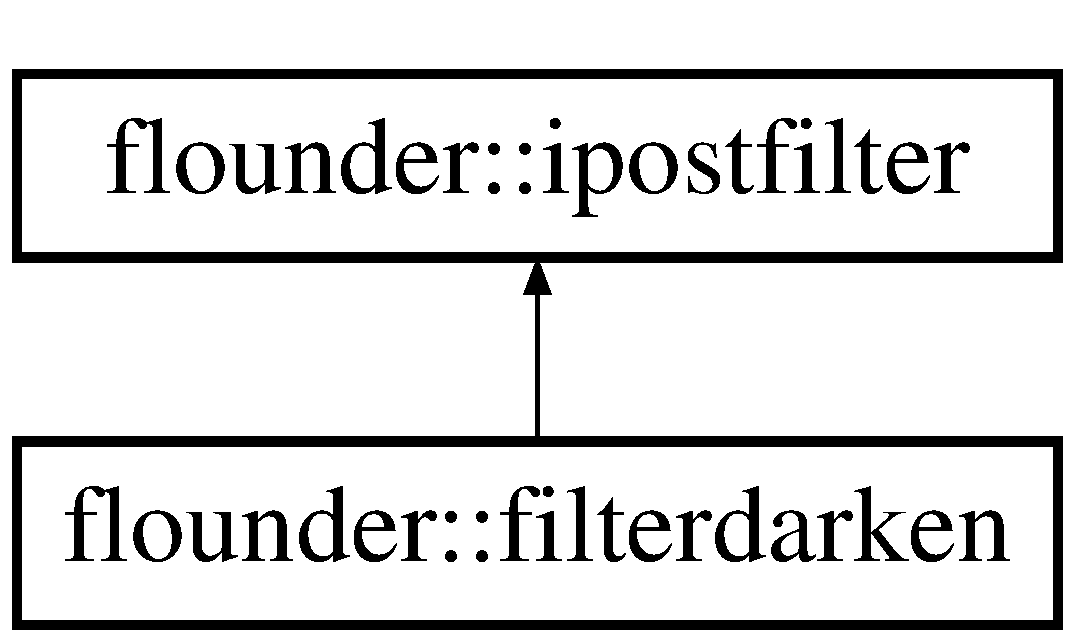
\includegraphics[height=2.000000cm]{classflounder_1_1filterdarken}
\end{center}
\end{figure}
\subsection*{Public Member Functions}
\begin{DoxyCompactItemize}
\item 
\mbox{\Hypertarget{classflounder_1_1filterdarken_a89b9c01e377def190a9174e9f7209682}\label{classflounder_1_1filterdarken_a89b9c01e377def190a9174e9f7209682}} 
{\bfseries filterdarken} (const float \&factor\+Value)
\item 
void \hyperlink{classflounder_1_1filterdarken_a5cee7990cb4de781465cf43f4695e823}{store\+Values} () override
\begin{DoxyCompactList}\small\item\em Can be used to store values into the shader, this is called when the filter is applied and the shader has been already started. \end{DoxyCompactList}\item 
\mbox{\Hypertarget{classflounder_1_1filterdarken_ad78cb798abfe2e4f0f0c5356fbf4aba6}\label{classflounder_1_1filterdarken_ad78cb798abfe2e4f0f0c5356fbf4aba6}} 
void {\bfseries set\+Factor\+Value} (const float \&factor\+Value)
\end{DoxyCompactItemize}
\subsection*{Private Attributes}
\begin{DoxyCompactItemize}
\item 
\mbox{\Hypertarget{classflounder_1_1filterdarken_a43f1497c8d60f906b1290152231bc4dc}\label{classflounder_1_1filterdarken_a43f1497c8d60f906b1290152231bc4dc}} 
float {\bfseries m\+\_\+factor\+Value}
\end{DoxyCompactItemize}
\subsection*{Additional Inherited Members}


\subsection{Member Function Documentation}
\mbox{\Hypertarget{classflounder_1_1filterdarken_a5cee7990cb4de781465cf43f4695e823}\label{classflounder_1_1filterdarken_a5cee7990cb4de781465cf43f4695e823}} 
\index{flounder\+::filterdarken@{flounder\+::filterdarken}!store\+Values@{store\+Values}}
\index{store\+Values@{store\+Values}!flounder\+::filterdarken@{flounder\+::filterdarken}}
\subsubsection{\texorpdfstring{store\+Values()}{storeValues()}}
{\footnotesize\ttfamily void flounder\+::filterdarken\+::store\+Values (\begin{DoxyParamCaption}{ }\end{DoxyParamCaption})\hspace{0.3cm}{\ttfamily [override]}, {\ttfamily [virtual]}}



Can be used to store values into the shader, this is called when the filter is applied and the shader has been already started. 



Implements \hyperlink{classflounder_1_1ipostfilter_a9b658b4672718d5ac36539875bde722e}{flounder\+::ipostfilter}.



The documentation for this class was generated from the following files\+:\begin{DoxyCompactItemize}
\item 
Flounder-\/\+Core/src/post/filters/filterdarken.\+h\item 
Flounder-\/\+Core/src/post/filters/filterdarken.\+cpp\end{DoxyCompactItemize}

\hypertarget{classflounder_1_1filterdefault}{}\section{flounder\+:\+:filterdefault Class Reference}
\label{classflounder_1_1filterdefault}\index{flounder\+::filterdefault@{flounder\+::filterdefault}}
Inheritance diagram for flounder\+:\+:filterdefault\+:\begin{figure}[H]
\begin{center}
\leavevmode
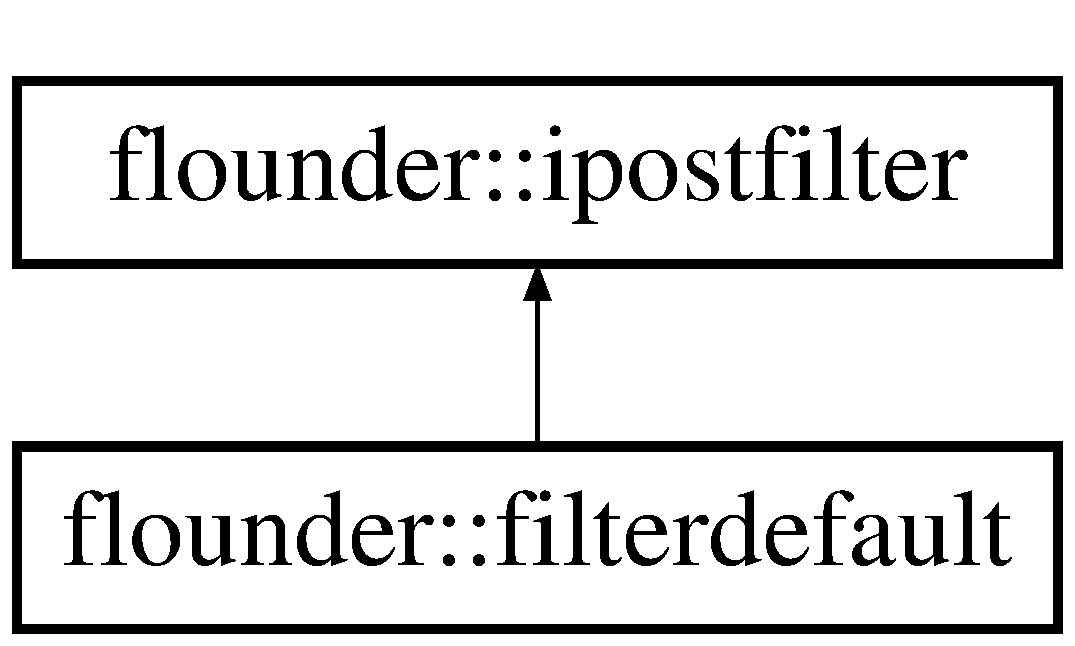
\includegraphics[height=2.000000cm]{classflounder_1_1filterdefault}
\end{center}
\end{figure}
\subsection*{Public Member Functions}
\begin{DoxyCompactItemize}
\item 
void \hyperlink{classflounder_1_1filterdefault_a9e858528a7d3356b94e16f10928a1d72}{store\+Values} () override
\begin{DoxyCompactList}\small\item\em Can be used to store values into the shader, this is called when the filter is applied and the shader has been already started. \end{DoxyCompactList}\end{DoxyCompactItemize}
\subsection*{Additional Inherited Members}


\subsection{Member Function Documentation}
\mbox{\Hypertarget{classflounder_1_1filterdefault_a9e858528a7d3356b94e16f10928a1d72}\label{classflounder_1_1filterdefault_a9e858528a7d3356b94e16f10928a1d72}} 
\index{flounder\+::filterdefault@{flounder\+::filterdefault}!store\+Values@{store\+Values}}
\index{store\+Values@{store\+Values}!flounder\+::filterdefault@{flounder\+::filterdefault}}
\subsubsection{\texorpdfstring{store\+Values()}{storeValues()}}
{\footnotesize\ttfamily void flounder\+::filterdefault\+::store\+Values (\begin{DoxyParamCaption}{ }\end{DoxyParamCaption})\hspace{0.3cm}{\ttfamily [override]}, {\ttfamily [virtual]}}



Can be used to store values into the shader, this is called when the filter is applied and the shader has been already started. 



Implements \hyperlink{classflounder_1_1ipostfilter_a9b658b4672718d5ac36539875bde722e}{flounder\+::ipostfilter}.



The documentation for this class was generated from the following files\+:\begin{DoxyCompactItemize}
\item 
Flounder-\/\+Core/src/post/filters/filterdefault.\+h\item 
Flounder-\/\+Core/src/post/filters/filterdefault.\+cpp\end{DoxyCompactItemize}

\hypertarget{classflounder_1_1filteremboss}{}\section{flounder\+:\+:filteremboss Class Reference}
\label{classflounder_1_1filteremboss}\index{flounder\+::filteremboss@{flounder\+::filteremboss}}
Inheritance diagram for flounder\+:\+:filteremboss\+:\begin{figure}[H]
\begin{center}
\leavevmode
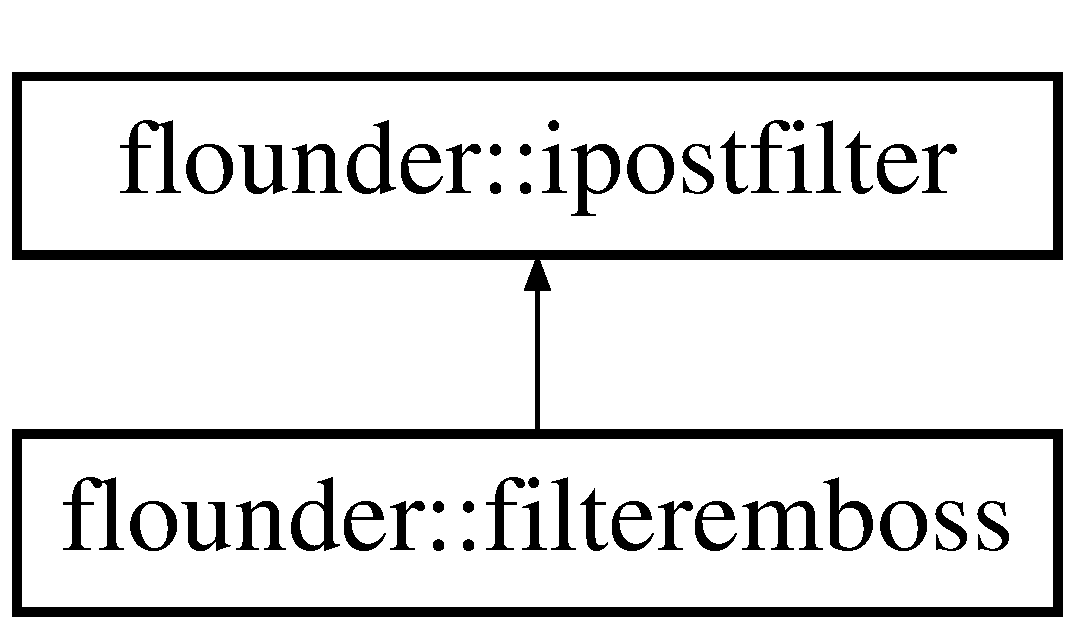
\includegraphics[height=2.000000cm]{classflounder_1_1filteremboss}
\end{center}
\end{figure}
\subsection*{Public Member Functions}
\begin{DoxyCompactItemize}
\item 
void \hyperlink{classflounder_1_1filteremboss_aa0c7d249c2c830036904bede59dababf}{store\+Values} () override
\begin{DoxyCompactList}\small\item\em Can be used to store values into the shader, this is called when the filter is applied and the shader has been already started. \end{DoxyCompactList}\end{DoxyCompactItemize}
\subsection*{Additional Inherited Members}


\subsection{Member Function Documentation}
\mbox{\Hypertarget{classflounder_1_1filteremboss_aa0c7d249c2c830036904bede59dababf}\label{classflounder_1_1filteremboss_aa0c7d249c2c830036904bede59dababf}} 
\index{flounder\+::filteremboss@{flounder\+::filteremboss}!store\+Values@{store\+Values}}
\index{store\+Values@{store\+Values}!flounder\+::filteremboss@{flounder\+::filteremboss}}
\subsubsection{\texorpdfstring{store\+Values()}{storeValues()}}
{\footnotesize\ttfamily void flounder\+::filteremboss\+::store\+Values (\begin{DoxyParamCaption}{ }\end{DoxyParamCaption})\hspace{0.3cm}{\ttfamily [override]}, {\ttfamily [virtual]}}



Can be used to store values into the shader, this is called when the filter is applied and the shader has been already started. 



Implements \hyperlink{classflounder_1_1ipostfilter_a9b658b4672718d5ac36539875bde722e}{flounder\+::ipostfilter}.



The documentation for this class was generated from the following files\+:\begin{DoxyCompactItemize}
\item 
Flounder-\/\+Core/src/post/filters/filteremboss.\+h\item 
Flounder-\/\+Core/src/post/filters/filteremboss.\+cpp\end{DoxyCompactItemize}

\hypertarget{classflounder_1_1filterfxaa}{}\section{flounder\+:\+:filterfxaa Class Reference}
\label{classflounder_1_1filterfxaa}\index{flounder\+::filterfxaa@{flounder\+::filterfxaa}}
Inheritance diagram for flounder\+:\+:filterfxaa\+:\begin{figure}[H]
\begin{center}
\leavevmode
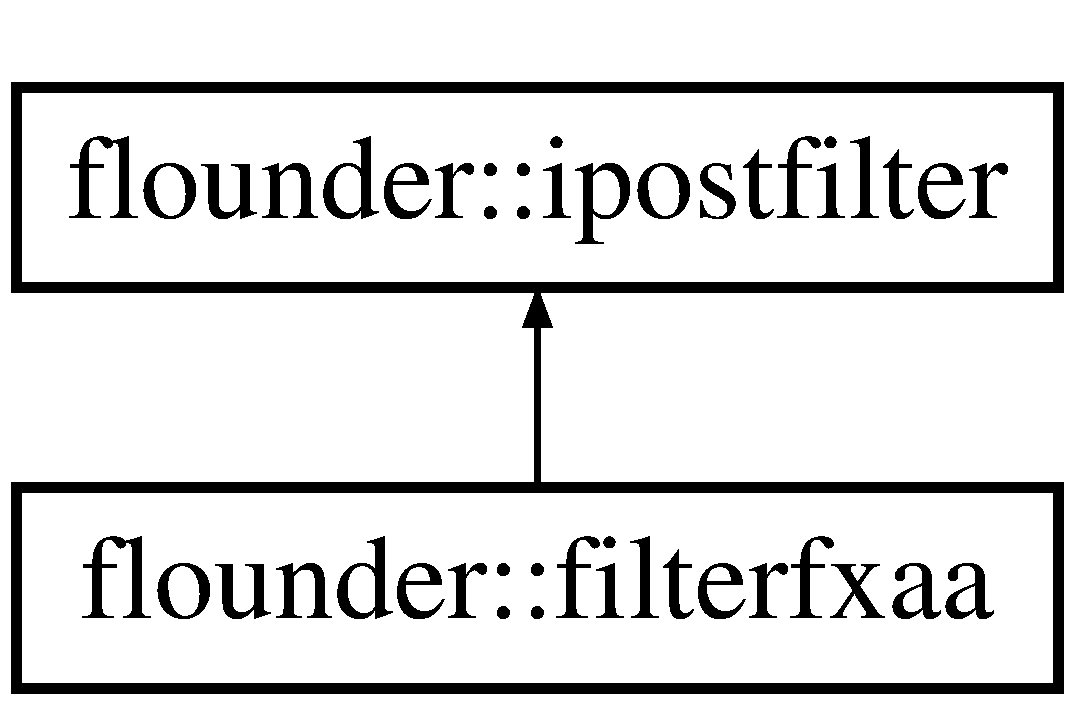
\includegraphics[height=2.000000cm]{classflounder_1_1filterfxaa}
\end{center}
\end{figure}
\subsection*{Public Member Functions}
\begin{DoxyCompactItemize}
\item 
\mbox{\Hypertarget{classflounder_1_1filterfxaa_aedc837c39551ff54c89704d3f14975e1}\label{classflounder_1_1filterfxaa_aedc837c39551ff54c89704d3f14975e1}} 
{\bfseries filterfxaa} (const float \&span\+Max)
\item 
void \hyperlink{classflounder_1_1filterfxaa_abee255cfd538d96881386157e6e8eea0}{store\+Values} () override
\begin{DoxyCompactList}\small\item\em Can be used to store values into the shader, this is called when the filter is applied and the shader has been already started. \end{DoxyCompactList}\item 
\mbox{\Hypertarget{classflounder_1_1filterfxaa_a8ff0740ed5a503f108e6b0b73e8e36f8}\label{classflounder_1_1filterfxaa_a8ff0740ed5a503f108e6b0b73e8e36f8}} 
float {\bfseries get\+Span\+Max} ()
\item 
\mbox{\Hypertarget{classflounder_1_1filterfxaa_a0d3b09024e4966bdafecbc5b388cc129}\label{classflounder_1_1filterfxaa_a0d3b09024e4966bdafecbc5b388cc129}} 
void {\bfseries set\+Span\+Max} (const float \&span\+Max)
\end{DoxyCompactItemize}
\subsection*{Private Attributes}
\begin{DoxyCompactItemize}
\item 
\mbox{\Hypertarget{classflounder_1_1filterfxaa_a6f59a5c3990455c2ddb30e2df9e1a140}\label{classflounder_1_1filterfxaa_a6f59a5c3990455c2ddb30e2df9e1a140}} 
float {\bfseries m\+\_\+span\+Max}
\end{DoxyCompactItemize}
\subsection*{Additional Inherited Members}


\subsection{Member Function Documentation}
\mbox{\Hypertarget{classflounder_1_1filterfxaa_abee255cfd538d96881386157e6e8eea0}\label{classflounder_1_1filterfxaa_abee255cfd538d96881386157e6e8eea0}} 
\index{flounder\+::filterfxaa@{flounder\+::filterfxaa}!store\+Values@{store\+Values}}
\index{store\+Values@{store\+Values}!flounder\+::filterfxaa@{flounder\+::filterfxaa}}
\subsubsection{\texorpdfstring{store\+Values()}{storeValues()}}
{\footnotesize\ttfamily void flounder\+::filterfxaa\+::store\+Values (\begin{DoxyParamCaption}{ }\end{DoxyParamCaption})\hspace{0.3cm}{\ttfamily [override]}, {\ttfamily [virtual]}}



Can be used to store values into the shader, this is called when the filter is applied and the shader has been already started. 



Implements \hyperlink{classflounder_1_1ipostfilter_a9b658b4672718d5ac36539875bde722e}{flounder\+::ipostfilter}.



The documentation for this class was generated from the following files\+:\begin{DoxyCompactItemize}
\item 
C\+:/\+Users/mattp/\+Documents/\+Flounder/\+Flounder\+Core/\+Sources/post/filters/filterfxaa.\+h\item 
C\+:/\+Users/mattp/\+Documents/\+Flounder/\+Flounder\+Core/\+Sources/post/filters/filterfxaa.\+cpp\end{DoxyCompactItemize}

\hypertarget{classflounder_1_1filtergrain}{}\section{flounder\+:\+:filtergrain Class Reference}
\label{classflounder_1_1filtergrain}\index{flounder\+::filtergrain@{flounder\+::filtergrain}}
Inheritance diagram for flounder\+:\+:filtergrain\+:\begin{figure}[H]
\begin{center}
\leavevmode
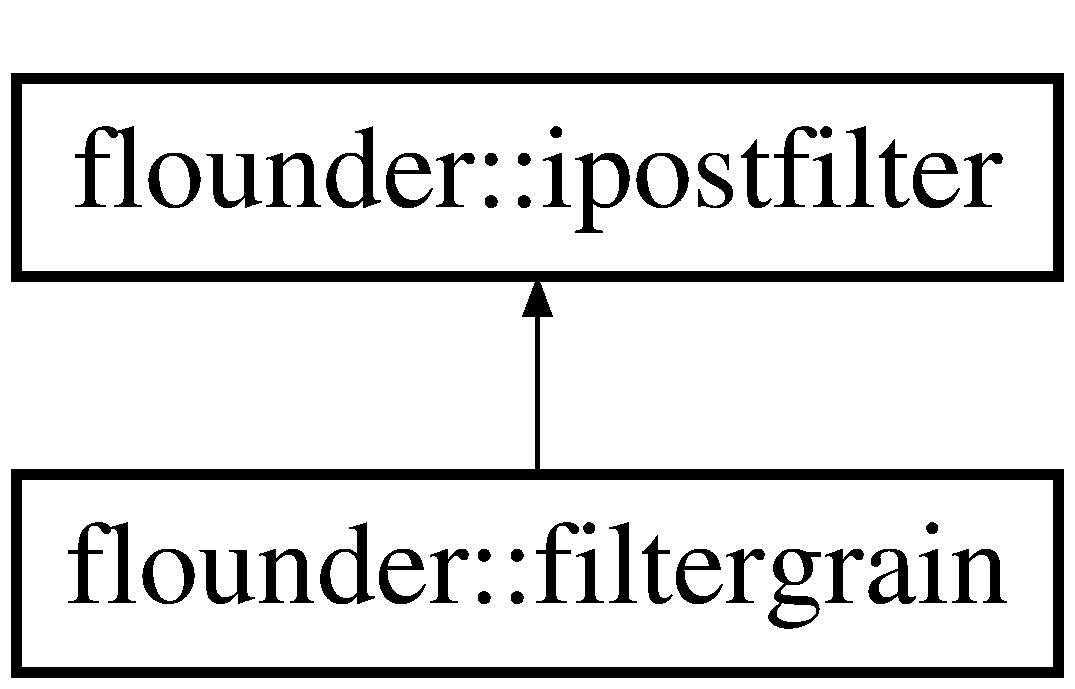
\includegraphics[height=2.000000cm]{classflounder_1_1filtergrain}
\end{center}
\end{figure}
\subsection*{Public Member Functions}
\begin{DoxyCompactItemize}
\item 
\mbox{\Hypertarget{classflounder_1_1filtergrain_aea807307ca6342c08b8a301ea2dd00c0}\label{classflounder_1_1filtergrain_aea807307ca6342c08b8a301ea2dd00c0}} 
{\bfseries filtergrain} (const float \&strength)
\item 
void \hyperlink{classflounder_1_1filtergrain_a0f65f9e8b994f18a4777e4451bdf8b4e}{store\+Values} () override
\begin{DoxyCompactList}\small\item\em Can be used to store values into the shader, this is called when the filter is applied and the shader has been already started. \end{DoxyCompactList}\item 
\mbox{\Hypertarget{classflounder_1_1filtergrain_a6d0cc4aed59190316cb51ee163f4d644}\label{classflounder_1_1filtergrain_a6d0cc4aed59190316cb51ee163f4d644}} 
float {\bfseries get\+Strength} ()
\item 
\mbox{\Hypertarget{classflounder_1_1filtergrain_ac6f764272481963353642bd7b3d4f746}\label{classflounder_1_1filtergrain_ac6f764272481963353642bd7b3d4f746}} 
void {\bfseries set\+Strength} (const float \&strength)
\end{DoxyCompactItemize}
\subsection*{Private Attributes}
\begin{DoxyCompactItemize}
\item 
\mbox{\Hypertarget{classflounder_1_1filtergrain_a038e33f9dd08809f8242d67336ad4483}\label{classflounder_1_1filtergrain_a038e33f9dd08809f8242d67336ad4483}} 
float {\bfseries m\+\_\+strength}
\end{DoxyCompactItemize}
\subsection*{Additional Inherited Members}


\subsection{Member Function Documentation}
\mbox{\Hypertarget{classflounder_1_1filtergrain_a0f65f9e8b994f18a4777e4451bdf8b4e}\label{classflounder_1_1filtergrain_a0f65f9e8b994f18a4777e4451bdf8b4e}} 
\index{flounder\+::filtergrain@{flounder\+::filtergrain}!store\+Values@{store\+Values}}
\index{store\+Values@{store\+Values}!flounder\+::filtergrain@{flounder\+::filtergrain}}
\subsubsection{\texorpdfstring{store\+Values()}{storeValues()}}
{\footnotesize\ttfamily void flounder\+::filtergrain\+::store\+Values (\begin{DoxyParamCaption}{ }\end{DoxyParamCaption})\hspace{0.3cm}{\ttfamily [override]}, {\ttfamily [virtual]}}



Can be used to store values into the shader, this is called when the filter is applied and the shader has been already started. 



Implements \hyperlink{classflounder_1_1ipostfilter_a9b658b4672718d5ac36539875bde722e}{flounder\+::ipostfilter}.



The documentation for this class was generated from the following files\+:\begin{DoxyCompactItemize}
\item 
C\+:/\+Users/mattp/\+Documents/\+Flounder/\+Flounder\+Core/\+Sources/post/filters/filtergrain.\+h\item 
C\+:/\+Users/mattp/\+Documents/\+Flounder/\+Flounder\+Core/\+Sources/post/filters/filtergrain.\+cpp\end{DoxyCompactItemize}

\hypertarget{classflounder_1_1filtergrey}{}\section{flounder\+:\+:filtergrey Class Reference}
\label{classflounder_1_1filtergrey}\index{flounder\+::filtergrey@{flounder\+::filtergrey}}
Inheritance diagram for flounder\+:\+:filtergrey\+:\begin{figure}[H]
\begin{center}
\leavevmode
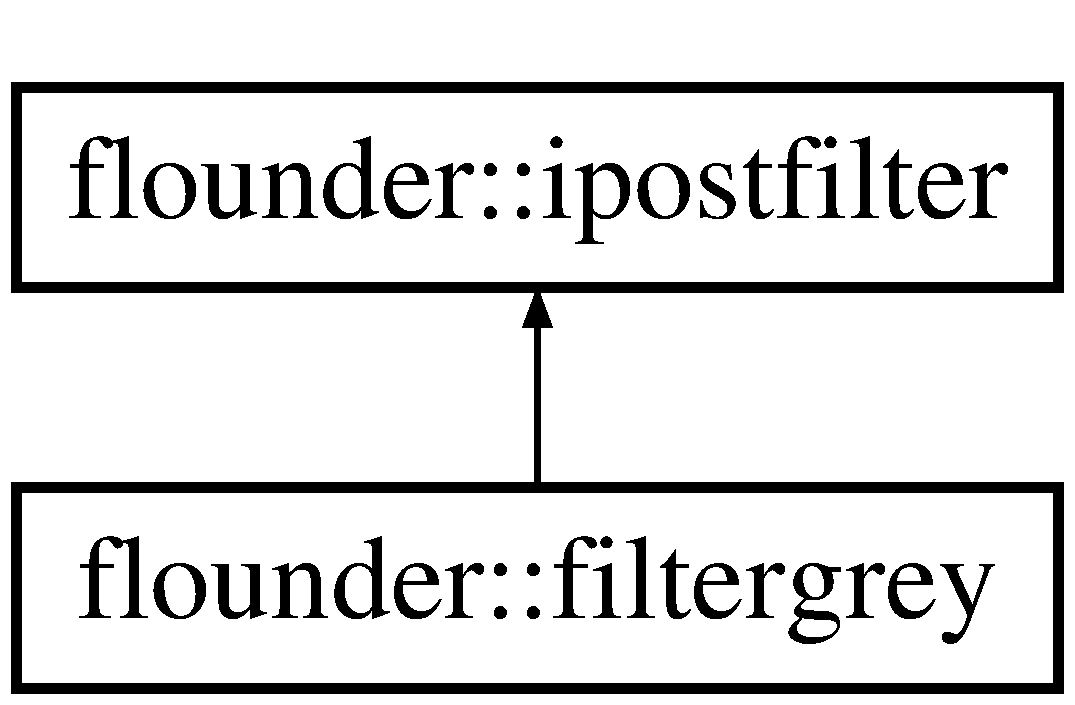
\includegraphics[height=2.000000cm]{classflounder_1_1filtergrey}
\end{center}
\end{figure}
\subsection*{Public Member Functions}
\begin{DoxyCompactItemize}
\item 
void \hyperlink{classflounder_1_1filtergrey_a927f448820b39299eb04c947ffdce671}{store\+Values} () override
\begin{DoxyCompactList}\small\item\em Can be used to store values into the shader, this is called when the filter is applied and the shader has been already started. \end{DoxyCompactList}\end{DoxyCompactItemize}
\subsection*{Additional Inherited Members}


\subsection{Member Function Documentation}
\mbox{\Hypertarget{classflounder_1_1filtergrey_a927f448820b39299eb04c947ffdce671}\label{classflounder_1_1filtergrey_a927f448820b39299eb04c947ffdce671}} 
\index{flounder\+::filtergrey@{flounder\+::filtergrey}!store\+Values@{store\+Values}}
\index{store\+Values@{store\+Values}!flounder\+::filtergrey@{flounder\+::filtergrey}}
\subsubsection{\texorpdfstring{store\+Values()}{storeValues()}}
{\footnotesize\ttfamily void flounder\+::filtergrey\+::store\+Values (\begin{DoxyParamCaption}{ }\end{DoxyParamCaption})\hspace{0.3cm}{\ttfamily [override]}, {\ttfamily [virtual]}}



Can be used to store values into the shader, this is called when the filter is applied and the shader has been already started. 



Implements \hyperlink{classflounder_1_1ipostfilter_a9b658b4672718d5ac36539875bde722e}{flounder\+::ipostfilter}.



The documentation for this class was generated from the following files\+:\begin{DoxyCompactItemize}
\item 
Flounder-\/\+Core/src/post/filters/filtergrey.\+h\item 
Flounder-\/\+Core/src/post/filters/filtergrey.\+cpp\end{DoxyCompactItemize}

\hypertarget{classflounder_1_1filterlensflare}{}\section{flounder\+:\+:filterlensflare Class Reference}
\label{classflounder_1_1filterlensflare}\index{flounder\+::filterlensflare@{flounder\+::filterlensflare}}
Inheritance diagram for flounder\+:\+:filterlensflare\+:\begin{figure}[H]
\begin{center}
\leavevmode
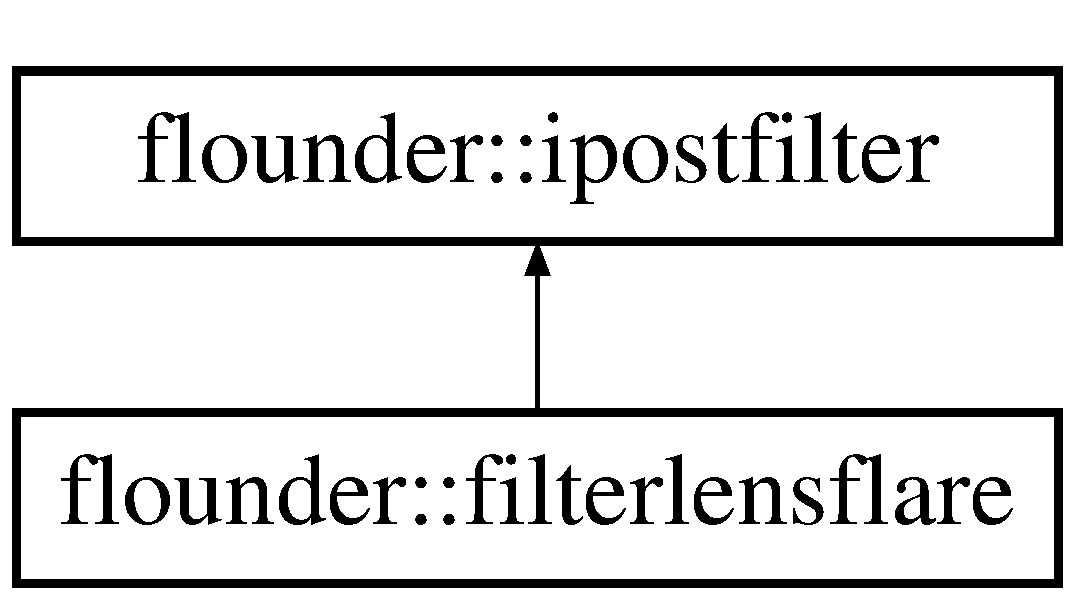
\includegraphics[height=2.000000cm]{classflounder_1_1filterlensflare}
\end{center}
\end{figure}
\subsection*{Public Member Functions}
\begin{DoxyCompactItemize}
\item 
void \hyperlink{classflounder_1_1filterlensflare_a2ab19cc2427e840c9ae11fc004e963be}{store\+Values} () override
\begin{DoxyCompactList}\small\item\em Can be used to store values into the shader, this is called when the filter is applied and the shader has been already started. \end{DoxyCompactList}\item 
\mbox{\Hypertarget{classflounder_1_1filterlensflare_acf8079971964f7e36d05fb96acddc9aa}\label{classflounder_1_1filterlensflare_acf8079971964f7e36d05fb96acddc9aa}} 
void {\bfseries set\+Sun\+Position} (const \hyperlink{classflounder_1_1vector3}{vector3} \&sun\+Position)
\item 
\mbox{\Hypertarget{classflounder_1_1filterlensflare_a3c3956ed82d5b68e5c577b8e3639b263}\label{classflounder_1_1filterlensflare_a3c3956ed82d5b68e5c577b8e3639b263}} 
void {\bfseries set\+Sun\+Height} (const float \&sun\+Height)
\end{DoxyCompactItemize}
\subsection*{Private Attributes}
\begin{DoxyCompactItemize}
\item 
\mbox{\Hypertarget{classflounder_1_1filterlensflare_aa437a3fdb68b06998eadfbd0e1067b63}\label{classflounder_1_1filterlensflare_aa437a3fdb68b06998eadfbd0e1067b63}} 
\hyperlink{classflounder_1_1vector3}{vector3} $\ast$ {\bfseries m\+\_\+sun\+Position}
\item 
\mbox{\Hypertarget{classflounder_1_1filterlensflare_a85a74873a0dc6b5f8886fb74a0760a1f}\label{classflounder_1_1filterlensflare_a85a74873a0dc6b5f8886fb74a0760a1f}} 
float {\bfseries m\+\_\+sun\+Height}
\end{DoxyCompactItemize}
\subsection*{Additional Inherited Members}


\subsection{Member Function Documentation}
\mbox{\Hypertarget{classflounder_1_1filterlensflare_a2ab19cc2427e840c9ae11fc004e963be}\label{classflounder_1_1filterlensflare_a2ab19cc2427e840c9ae11fc004e963be}} 
\index{flounder\+::filterlensflare@{flounder\+::filterlensflare}!store\+Values@{store\+Values}}
\index{store\+Values@{store\+Values}!flounder\+::filterlensflare@{flounder\+::filterlensflare}}
\subsubsection{\texorpdfstring{store\+Values()}{storeValues()}}
{\footnotesize\ttfamily void flounder\+::filterlensflare\+::store\+Values (\begin{DoxyParamCaption}{ }\end{DoxyParamCaption})\hspace{0.3cm}{\ttfamily [override]}, {\ttfamily [virtual]}}



Can be used to store values into the shader, this is called when the filter is applied and the shader has been already started. 



Implements \hyperlink{classflounder_1_1ipostfilter_a9b658b4672718d5ac36539875bde722e}{flounder\+::ipostfilter}.



The documentation for this class was generated from the following files\+:\begin{DoxyCompactItemize}
\item 
Flounder-\/\+Core/src/post/filters/filterlensflare.\+h\item 
Flounder-\/\+Core/src/post/filters/filterlensflare.\+cpp\end{DoxyCompactItemize}

\hypertarget{classflounder_1_1filtermotion}{}\section{flounder\+:\+:filtermotion Class Reference}
\label{classflounder_1_1filtermotion}\index{flounder\+::filtermotion@{flounder\+::filtermotion}}
Inheritance diagram for flounder\+:\+:filtermotion\+:\begin{figure}[H]
\begin{center}
\leavevmode
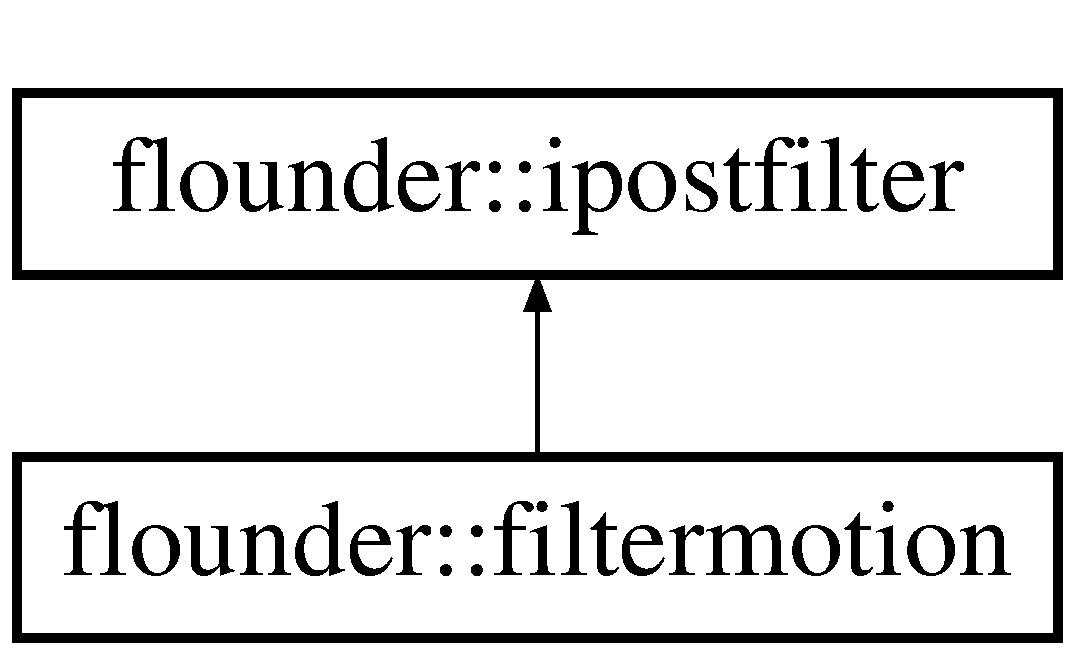
\includegraphics[height=2.000000cm]{classflounder_1_1filtermotion}
\end{center}
\end{figure}
\subsection*{Public Member Functions}
\begin{DoxyCompactItemize}
\item 
void \hyperlink{classflounder_1_1filtermotion_a6e8b5a9ce3660ab57fbb487fe6752acb}{store\+Values} () override
\begin{DoxyCompactList}\small\item\em Can be used to store values into the shader, this is called when the filter is applied and the shader has been already started. \end{DoxyCompactList}\end{DoxyCompactItemize}
\subsection*{Private Attributes}
\begin{DoxyCompactItemize}
\item 
\mbox{\Hypertarget{classflounder_1_1filtermotion_a3d2b6639e87b9e747f62a5ba0206b5fa}\label{classflounder_1_1filtermotion_a3d2b6639e87b9e747f62a5ba0206b5fa}} 
\hyperlink{classflounder_1_1matrix4x4}{matrix4x4} $\ast$ {\bfseries m\+\_\+last\+View\+Matrix}
\end{DoxyCompactItemize}
\subsection*{Additional Inherited Members}


\subsection{Member Function Documentation}
\mbox{\Hypertarget{classflounder_1_1filtermotion_a6e8b5a9ce3660ab57fbb487fe6752acb}\label{classflounder_1_1filtermotion_a6e8b5a9ce3660ab57fbb487fe6752acb}} 
\index{flounder\+::filtermotion@{flounder\+::filtermotion}!store\+Values@{store\+Values}}
\index{store\+Values@{store\+Values}!flounder\+::filtermotion@{flounder\+::filtermotion}}
\subsubsection{\texorpdfstring{store\+Values()}{storeValues()}}
{\footnotesize\ttfamily void flounder\+::filtermotion\+::store\+Values (\begin{DoxyParamCaption}{ }\end{DoxyParamCaption})\hspace{0.3cm}{\ttfamily [override]}, {\ttfamily [virtual]}}



Can be used to store values into the shader, this is called when the filter is applied and the shader has been already started. 



Implements \hyperlink{classflounder_1_1ipostfilter_a9b658b4672718d5ac36539875bde722e}{flounder\+::ipostfilter}.



The documentation for this class was generated from the following files\+:\begin{DoxyCompactItemize}
\item 
Flounder-\/\+Core/src/post/filters/filtermotion.\+h\item 
Flounder-\/\+Core/src/post/filters/filtermotion.\+cpp\end{DoxyCompactItemize}

\hypertarget{classflounder_1_1filternegative}{}\section{flounder\+:\+:filternegative Class Reference}
\label{classflounder_1_1filternegative}\index{flounder\+::filternegative@{flounder\+::filternegative}}
Inheritance diagram for flounder\+:\+:filternegative\+:\begin{figure}[H]
\begin{center}
\leavevmode
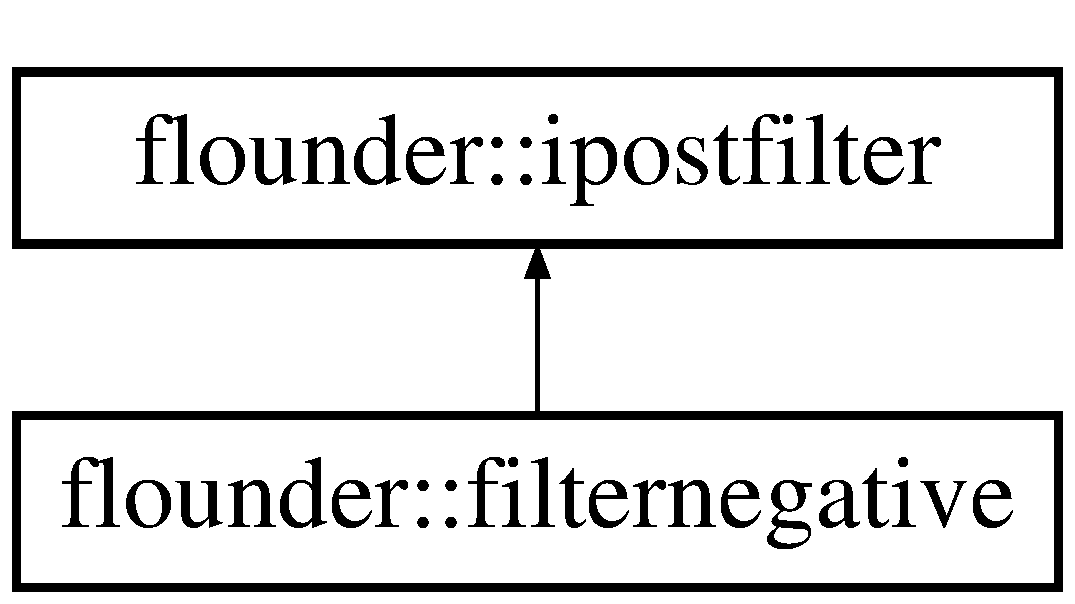
\includegraphics[height=2.000000cm]{classflounder_1_1filternegative}
\end{center}
\end{figure}
\subsection*{Public Member Functions}
\begin{DoxyCompactItemize}
\item 
void \hyperlink{classflounder_1_1filternegative_abc832140c4d75f4684d3470e070bcf7a}{store\+Values} () override
\begin{DoxyCompactList}\small\item\em Can be used to store values into the shader, this is called when the filter is applied and the shader has been already started. \end{DoxyCompactList}\end{DoxyCompactItemize}
\subsection*{Additional Inherited Members}


\subsection{Member Function Documentation}
\mbox{\Hypertarget{classflounder_1_1filternegative_abc832140c4d75f4684d3470e070bcf7a}\label{classflounder_1_1filternegative_abc832140c4d75f4684d3470e070bcf7a}} 
\index{flounder\+::filternegative@{flounder\+::filternegative}!store\+Values@{store\+Values}}
\index{store\+Values@{store\+Values}!flounder\+::filternegative@{flounder\+::filternegative}}
\subsubsection{\texorpdfstring{store\+Values()}{storeValues()}}
{\footnotesize\ttfamily void flounder\+::filternegative\+::store\+Values (\begin{DoxyParamCaption}{ }\end{DoxyParamCaption})\hspace{0.3cm}{\ttfamily [override]}, {\ttfamily [virtual]}}



Can be used to store values into the shader, this is called when the filter is applied and the shader has been already started. 



Implements \hyperlink{classflounder_1_1ipostfilter_a9b658b4672718d5ac36539875bde722e}{flounder\+::ipostfilter}.



The documentation for this class was generated from the following files\+:\begin{DoxyCompactItemize}
\item 
C\+:/\+Users/mattp/\+Documents/\+Flounder/\+Flounder\+Core/\+Sources/post/filters/filternegative.\+h\item 
C\+:/\+Users/mattp/\+Documents/\+Flounder/\+Flounder\+Core/\+Sources/post/filters/filternegative.\+cpp\end{DoxyCompactItemize}

\hypertarget{classflounder_1_1filterpixel}{}\section{flounder\+:\+:filterpixel Class Reference}
\label{classflounder_1_1filterpixel}\index{flounder\+::filterpixel@{flounder\+::filterpixel}}
Inheritance diagram for flounder\+:\+:filterpixel\+:\begin{figure}[H]
\begin{center}
\leavevmode
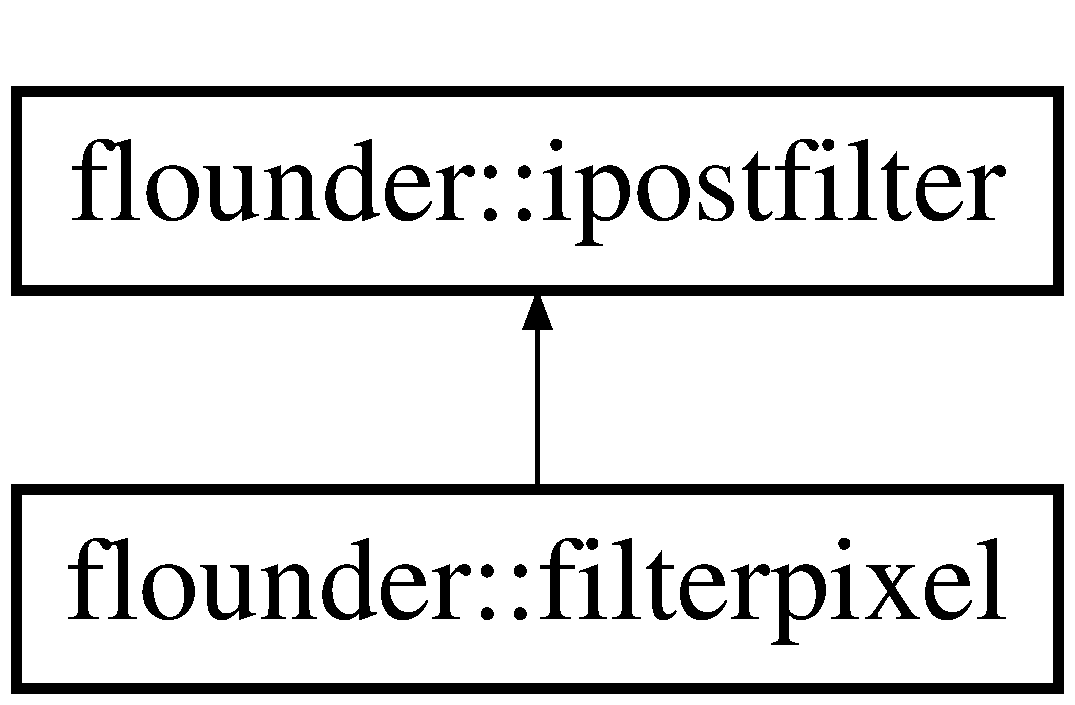
\includegraphics[height=2.000000cm]{classflounder_1_1filterpixel}
\end{center}
\end{figure}
\subsection*{Public Member Functions}
\begin{DoxyCompactItemize}
\item 
\mbox{\Hypertarget{classflounder_1_1filterpixel_aea7c2593620c495c641ab39031f10595}\label{classflounder_1_1filterpixel_aea7c2593620c495c641ab39031f10595}} 
{\bfseries filterpixel} (const float \&pixel\+Size)
\item 
void \hyperlink{classflounder_1_1filterpixel_abc7ae2b0a9bffd4986a664b690aab416}{store\+Values} () override
\begin{DoxyCompactList}\small\item\em Can be used to store values into the shader, this is called when the filter is applied and the shader has been already started. \end{DoxyCompactList}\item 
\mbox{\Hypertarget{classflounder_1_1filterpixel_a196e09572387085d6685f0451cc9cb91}\label{classflounder_1_1filterpixel_a196e09572387085d6685f0451cc9cb91}} 
void {\bfseries set\+Pixel\+Size} (const float \&pixel\+Size)
\end{DoxyCompactItemize}
\subsection*{Private Attributes}
\begin{DoxyCompactItemize}
\item 
\mbox{\Hypertarget{classflounder_1_1filterpixel_a01b9df1d3dd3f1854ae908c8dd0f1609}\label{classflounder_1_1filterpixel_a01b9df1d3dd3f1854ae908c8dd0f1609}} 
float {\bfseries m\+\_\+pixel\+Size}
\end{DoxyCompactItemize}
\subsection*{Additional Inherited Members}


\subsection{Member Function Documentation}
\mbox{\Hypertarget{classflounder_1_1filterpixel_abc7ae2b0a9bffd4986a664b690aab416}\label{classflounder_1_1filterpixel_abc7ae2b0a9bffd4986a664b690aab416}} 
\index{flounder\+::filterpixel@{flounder\+::filterpixel}!store\+Values@{store\+Values}}
\index{store\+Values@{store\+Values}!flounder\+::filterpixel@{flounder\+::filterpixel}}
\subsubsection{\texorpdfstring{store\+Values()}{storeValues()}}
{\footnotesize\ttfamily void flounder\+::filterpixel\+::store\+Values (\begin{DoxyParamCaption}{ }\end{DoxyParamCaption})\hspace{0.3cm}{\ttfamily [override]}, {\ttfamily [virtual]}}



Can be used to store values into the shader, this is called when the filter is applied and the shader has been already started. 



Implements \hyperlink{classflounder_1_1ipostfilter_a9b658b4672718d5ac36539875bde722e}{flounder\+::ipostfilter}.



The documentation for this class was generated from the following files\+:\begin{DoxyCompactItemize}
\item 
Flounder-\/\+Core/src/post/filters/filterpixel.\+h\item 
Flounder-\/\+Core/src/post/filters/filterpixel.\+cpp\end{DoxyCompactItemize}

\hypertarget{classflounder_1_1filtersepia}{}\section{flounder\+:\+:filtersepia Class Reference}
\label{classflounder_1_1filtersepia}\index{flounder\+::filtersepia@{flounder\+::filtersepia}}
Inheritance diagram for flounder\+:\+:filtersepia\+:\begin{figure}[H]
\begin{center}
\leavevmode
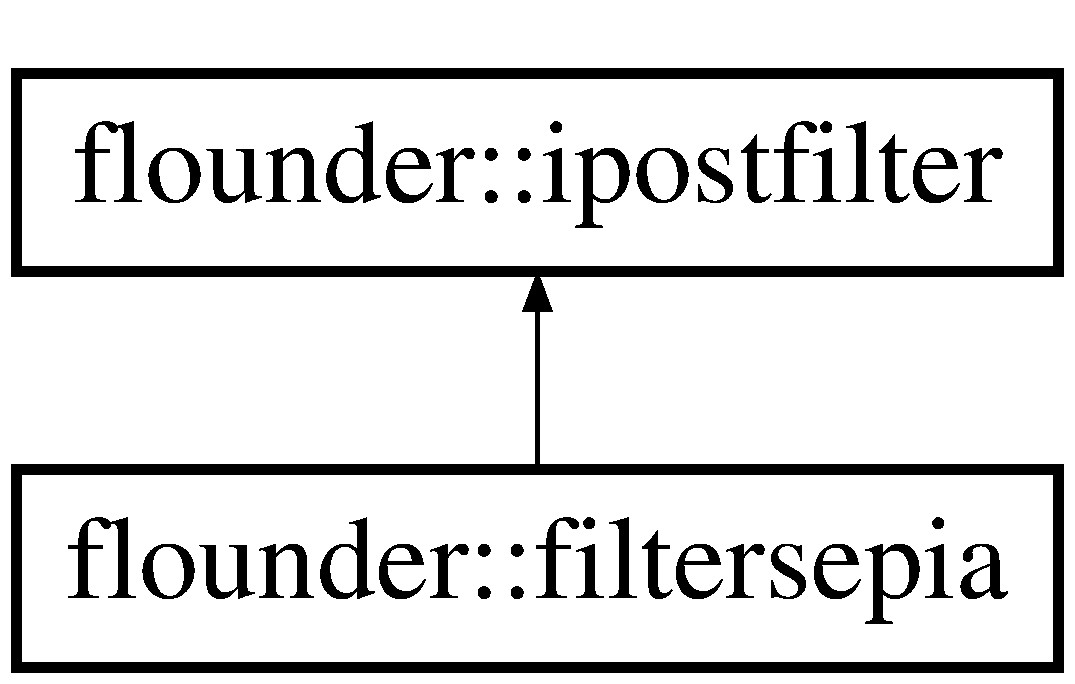
\includegraphics[height=2.000000cm]{classflounder_1_1filtersepia}
\end{center}
\end{figure}
\subsection*{Public Member Functions}
\begin{DoxyCompactItemize}
\item 
void \hyperlink{classflounder_1_1filtersepia_a92d9cee7e92200212f40ff39f5cbc67f}{store\+Values} () override
\begin{DoxyCompactList}\small\item\em Can be used to store values into the shader, this is called when the filter is applied and the shader has been already started. \end{DoxyCompactList}\end{DoxyCompactItemize}
\subsection*{Additional Inherited Members}


\subsection{Member Function Documentation}
\mbox{\Hypertarget{classflounder_1_1filtersepia_a92d9cee7e92200212f40ff39f5cbc67f}\label{classflounder_1_1filtersepia_a92d9cee7e92200212f40ff39f5cbc67f}} 
\index{flounder\+::filtersepia@{flounder\+::filtersepia}!store\+Values@{store\+Values}}
\index{store\+Values@{store\+Values}!flounder\+::filtersepia@{flounder\+::filtersepia}}
\subsubsection{\texorpdfstring{store\+Values()}{storeValues()}}
{\footnotesize\ttfamily void flounder\+::filtersepia\+::store\+Values (\begin{DoxyParamCaption}{ }\end{DoxyParamCaption})\hspace{0.3cm}{\ttfamily [override]}, {\ttfamily [virtual]}}



Can be used to store values into the shader, this is called when the filter is applied and the shader has been already started. 



Implements \hyperlink{classflounder_1_1ipostfilter_a9b658b4672718d5ac36539875bde722e}{flounder\+::ipostfilter}.



The documentation for this class was generated from the following files\+:\begin{DoxyCompactItemize}
\item 
Flounder-\/\+Core/src/post/filters/filtersepia.\+h\item 
Flounder-\/\+Core/src/post/filters/filtersepia.\+cpp\end{DoxyCompactItemize}

\hypertarget{classflounder_1_1filtertiltshift}{}\section{flounder\+:\+:filtertiltshift Class Reference}
\label{classflounder_1_1filtertiltshift}\index{flounder\+::filtertiltshift@{flounder\+::filtertiltshift}}
Inheritance diagram for flounder\+:\+:filtertiltshift\+:\begin{figure}[H]
\begin{center}
\leavevmode
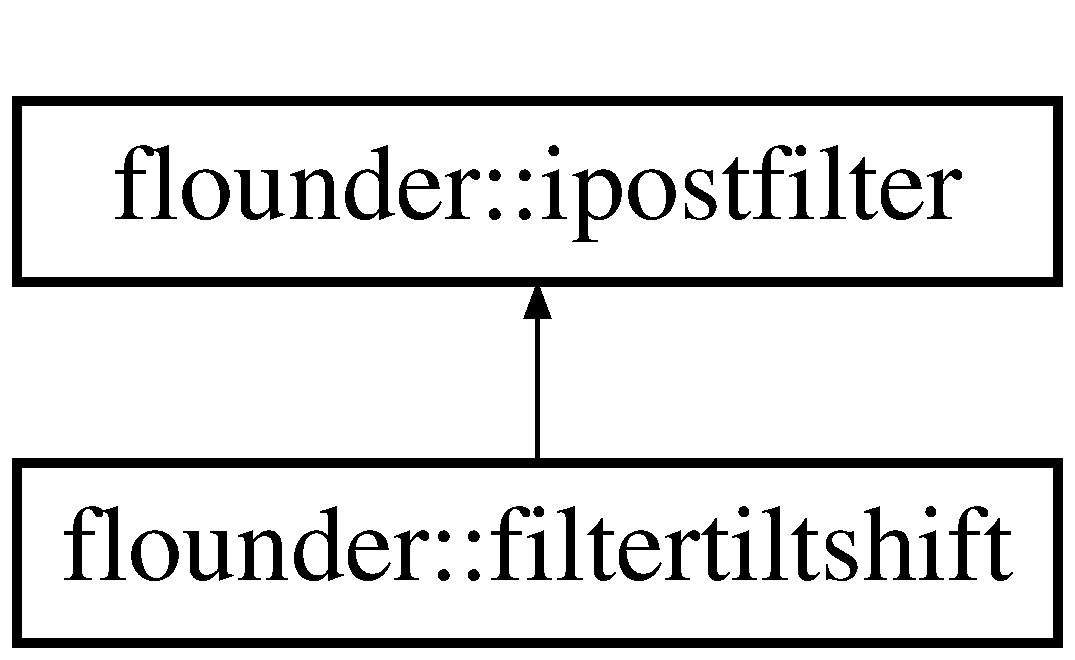
\includegraphics[height=2.000000cm]{classflounder_1_1filtertiltshift}
\end{center}
\end{figure}
\subsection*{Public Member Functions}
\begin{DoxyCompactItemize}
\item 
\mbox{\Hypertarget{classflounder_1_1filtertiltshift_acdbc3c02bf3fe5314910e2ebb257d6db}\label{classflounder_1_1filtertiltshift_acdbc3c02bf3fe5314910e2ebb257d6db}} 
{\bfseries filtertiltshift} (const float \&blur\+Amount, const float \&centre, const float \&step\+Size, const float \&steps)
\item 
void \hyperlink{classflounder_1_1filtertiltshift_a8e04e52da882a2d78d7a0e1f70717114}{store\+Values} () override
\begin{DoxyCompactList}\small\item\em Can be used to store values into the shader, this is called when the filter is applied and the shader has been already started. \end{DoxyCompactList}\item 
\mbox{\Hypertarget{classflounder_1_1filtertiltshift_a9064ec6b0c0e487906c05d494bf6512c}\label{classflounder_1_1filtertiltshift_a9064ec6b0c0e487906c05d494bf6512c}} 
void {\bfseries set\+Blur\+Amount} (const float \&blur\+Amount)
\item 
\mbox{\Hypertarget{classflounder_1_1filtertiltshift_ac45be454076e04bc350870eacb645b82}\label{classflounder_1_1filtertiltshift_ac45be454076e04bc350870eacb645b82}} 
void {\bfseries set\+Centre} (const float \&centre)
\item 
\mbox{\Hypertarget{classflounder_1_1filtertiltshift_a013a784c2e5a9703ce93420b45e06120}\label{classflounder_1_1filtertiltshift_a013a784c2e5a9703ce93420b45e06120}} 
void {\bfseries set\+Step\+Size} (const float \&step\+Size)
\item 
\mbox{\Hypertarget{classflounder_1_1filtertiltshift_a844d3051718025c35600ce7a79e01b89}\label{classflounder_1_1filtertiltshift_a844d3051718025c35600ce7a79e01b89}} 
void {\bfseries set\+Steps} (const float \&steps)
\end{DoxyCompactItemize}
\subsection*{Private Attributes}
\begin{DoxyCompactItemize}
\item 
\mbox{\Hypertarget{classflounder_1_1filtertiltshift_aaeab734f3a161f674e0f19069b4dc2da}\label{classflounder_1_1filtertiltshift_aaeab734f3a161f674e0f19069b4dc2da}} 
float {\bfseries m\+\_\+blur\+Amount}
\item 
\mbox{\Hypertarget{classflounder_1_1filtertiltshift_aa443e2cd33ed1d98355c368537d8dc11}\label{classflounder_1_1filtertiltshift_aa443e2cd33ed1d98355c368537d8dc11}} 
float {\bfseries m\+\_\+centre}
\item 
\mbox{\Hypertarget{classflounder_1_1filtertiltshift_a1e7f7d4bf90dbf93ecc9d27b159d390a}\label{classflounder_1_1filtertiltshift_a1e7f7d4bf90dbf93ecc9d27b159d390a}} 
float {\bfseries m\+\_\+step\+Size}
\item 
\mbox{\Hypertarget{classflounder_1_1filtertiltshift_afaa06de28aa7abf9c70d38c7dedc164c}\label{classflounder_1_1filtertiltshift_afaa06de28aa7abf9c70d38c7dedc164c}} 
float {\bfseries m\+\_\+steps}
\end{DoxyCompactItemize}
\subsection*{Additional Inherited Members}


\subsection{Member Function Documentation}
\mbox{\Hypertarget{classflounder_1_1filtertiltshift_a8e04e52da882a2d78d7a0e1f70717114}\label{classflounder_1_1filtertiltshift_a8e04e52da882a2d78d7a0e1f70717114}} 
\index{flounder\+::filtertiltshift@{flounder\+::filtertiltshift}!store\+Values@{store\+Values}}
\index{store\+Values@{store\+Values}!flounder\+::filtertiltshift@{flounder\+::filtertiltshift}}
\subsubsection{\texorpdfstring{store\+Values()}{storeValues()}}
{\footnotesize\ttfamily void flounder\+::filtertiltshift\+::store\+Values (\begin{DoxyParamCaption}{ }\end{DoxyParamCaption})\hspace{0.3cm}{\ttfamily [override]}, {\ttfamily [virtual]}}



Can be used to store values into the shader, this is called when the filter is applied and the shader has been already started. 



Implements \hyperlink{classflounder_1_1ipostfilter_a9b658b4672718d5ac36539875bde722e}{flounder\+::ipostfilter}.



The documentation for this class was generated from the following files\+:\begin{DoxyCompactItemize}
\item 
Flounder-\/\+Core/src/post/filters/filtertiltshift.\+h\item 
Flounder-\/\+Core/src/post/filters/filtertiltshift.\+cpp\end{DoxyCompactItemize}

\hypertarget{classflounder_1_1filtertone}{}\section{flounder\+:\+:filtertone Class Reference}
\label{classflounder_1_1filtertone}\index{flounder\+::filtertone@{flounder\+::filtertone}}
Inheritance diagram for flounder\+:\+:filtertone\+:\begin{figure}[H]
\begin{center}
\leavevmode
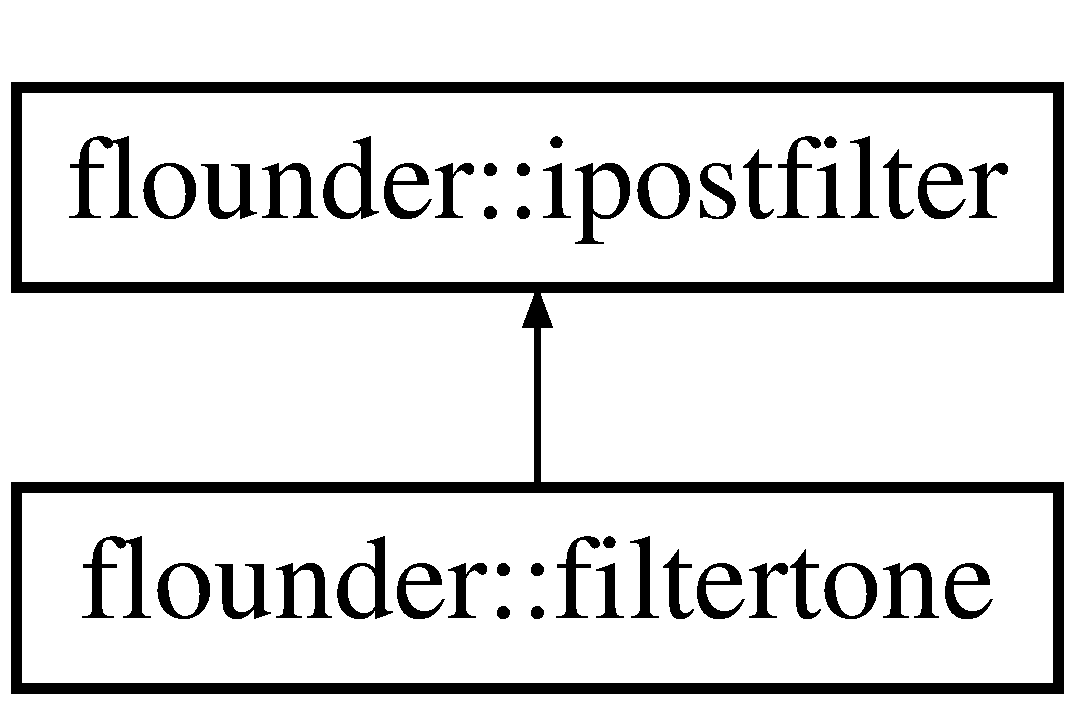
\includegraphics[height=2.000000cm]{classflounder_1_1filtertone}
\end{center}
\end{figure}
\subsection*{Public Member Functions}
\begin{DoxyCompactItemize}
\item 
void \hyperlink{classflounder_1_1filtertone_ad2b3b402d4f9fd38f918b410652ee96b}{store\+Values} () override
\begin{DoxyCompactList}\small\item\em Can be used to store values into the shader, this is called when the filter is applied and the shader has been already started. \end{DoxyCompactList}\end{DoxyCompactItemize}
\subsection*{Additional Inherited Members}


\subsection{Member Function Documentation}
\mbox{\Hypertarget{classflounder_1_1filtertone_ad2b3b402d4f9fd38f918b410652ee96b}\label{classflounder_1_1filtertone_ad2b3b402d4f9fd38f918b410652ee96b}} 
\index{flounder\+::filtertone@{flounder\+::filtertone}!store\+Values@{store\+Values}}
\index{store\+Values@{store\+Values}!flounder\+::filtertone@{flounder\+::filtertone}}
\subsubsection{\texorpdfstring{store\+Values()}{storeValues()}}
{\footnotesize\ttfamily void flounder\+::filtertone\+::store\+Values (\begin{DoxyParamCaption}{ }\end{DoxyParamCaption})\hspace{0.3cm}{\ttfamily [override]}, {\ttfamily [virtual]}}



Can be used to store values into the shader, this is called when the filter is applied and the shader has been already started. 



Implements \hyperlink{classflounder_1_1ipostfilter_a9b658b4672718d5ac36539875bde722e}{flounder\+::ipostfilter}.



The documentation for this class was generated from the following files\+:\begin{DoxyCompactItemize}
\item 
Flounder-\/\+Core/src/post/filters/filtertone.\+h\item 
Flounder-\/\+Core/src/post/filters/filtertone.\+cpp\end{DoxyCompactItemize}

\hypertarget{classflounder_1_1filterwobble}{}\section{flounder\+:\+:filterwobble Class Reference}
\label{classflounder_1_1filterwobble}\index{flounder\+::filterwobble@{flounder\+::filterwobble}}
Inheritance diagram for flounder\+:\+:filterwobble\+:\begin{figure}[H]
\begin{center}
\leavevmode
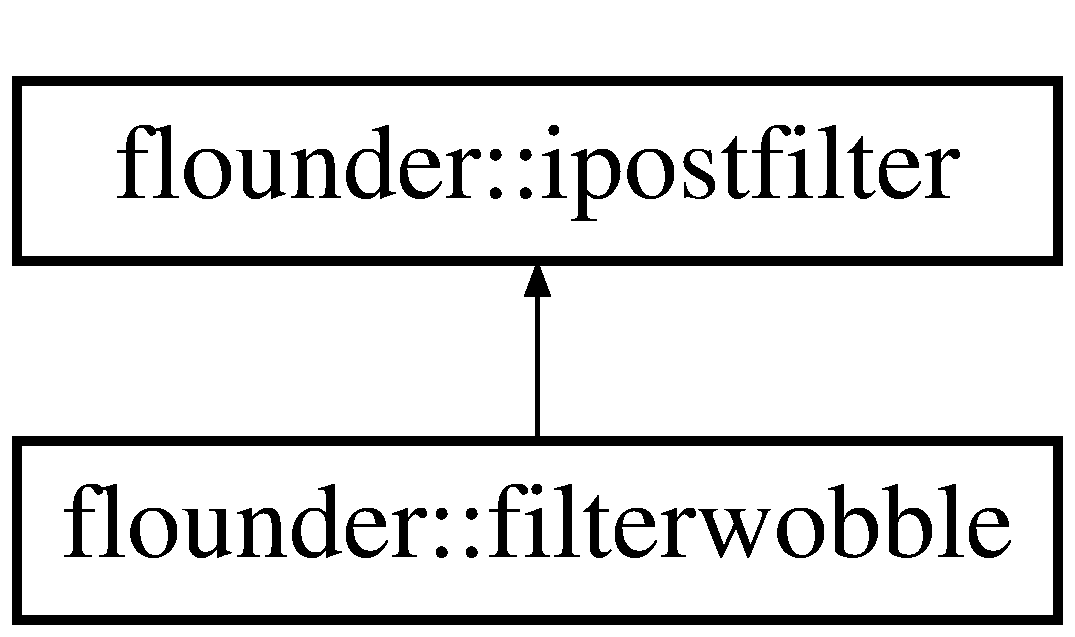
\includegraphics[height=2.000000cm]{classflounder_1_1filterwobble}
\end{center}
\end{figure}
\subsection*{Public Member Functions}
\begin{DoxyCompactItemize}
\item 
\mbox{\Hypertarget{classflounder_1_1filterwobble_a1652b7755d6405c677bfa8ce59dbb1ea}\label{classflounder_1_1filterwobble_a1652b7755d6405c677bfa8ce59dbb1ea}} 
{\bfseries filterwobble} (const float \&wobble\+Speed)
\item 
void \hyperlink{classflounder_1_1filterwobble_aa89ed7a9f3ad52790223b558aaff0cc4}{store\+Values} () override
\begin{DoxyCompactList}\small\item\em Can be used to store values into the shader, this is called when the filter is applied and the shader has been already started. \end{DoxyCompactList}\item 
\mbox{\Hypertarget{classflounder_1_1filterwobble_a4d1c42d560002f4deaab0f59766e191e}\label{classflounder_1_1filterwobble_a4d1c42d560002f4deaab0f59766e191e}} 
void {\bfseries set\+Wobble\+Speed} (const float \&wobble\+Speed)
\end{DoxyCompactItemize}
\subsection*{Private Attributes}
\begin{DoxyCompactItemize}
\item 
\mbox{\Hypertarget{classflounder_1_1filterwobble_ac10ce8e0eda476dcaae1a5ff9d838171}\label{classflounder_1_1filterwobble_ac10ce8e0eda476dcaae1a5ff9d838171}} 
float {\bfseries m\+\_\+wobble\+Speed}
\item 
\mbox{\Hypertarget{classflounder_1_1filterwobble_a7680465eea629d117dc88c0eec11a5bd}\label{classflounder_1_1filterwobble_a7680465eea629d117dc88c0eec11a5bd}} 
float {\bfseries m\+\_\+wobble\+Amount}
\end{DoxyCompactItemize}
\subsection*{Additional Inherited Members}


\subsection{Member Function Documentation}
\mbox{\Hypertarget{classflounder_1_1filterwobble_aa89ed7a9f3ad52790223b558aaff0cc4}\label{classflounder_1_1filterwobble_aa89ed7a9f3ad52790223b558aaff0cc4}} 
\index{flounder\+::filterwobble@{flounder\+::filterwobble}!store\+Values@{store\+Values}}
\index{store\+Values@{store\+Values}!flounder\+::filterwobble@{flounder\+::filterwobble}}
\subsubsection{\texorpdfstring{store\+Values()}{storeValues()}}
{\footnotesize\ttfamily void flounder\+::filterwobble\+::store\+Values (\begin{DoxyParamCaption}{ }\end{DoxyParamCaption})\hspace{0.3cm}{\ttfamily [override]}, {\ttfamily [virtual]}}



Can be used to store values into the shader, this is called when the filter is applied and the shader has been already started. 



Implements \hyperlink{classflounder_1_1ipostfilter_a9b658b4672718d5ac36539875bde722e}{flounder\+::ipostfilter}.



The documentation for this class was generated from the following files\+:\begin{DoxyCompactItemize}
\item 
Flounder-\/\+Core/src/post/filters/filterwobble.\+h\item 
Flounder-\/\+Core/src/post/filters/filterwobble.\+cpp\end{DoxyCompactItemize}

\hypertarget{classflounder_1_1fog}{}\section{flounder\+:\+:fog Class Reference}
\label{classflounder_1_1fog}\index{flounder\+::fog@{flounder\+::fog}}


Represents a fog in the world.  




{\ttfamily \#include $<$fog.\+h$>$}

\subsection*{Public Member Functions}
\begin{DoxyCompactItemize}
\item 
\hyperlink{classflounder_1_1fog_ae55a228dc40e89b3ab5077c81a7d1281}{fog} (\hyperlink{classflounder_1_1colour}{colour} $\ast$\hyperlink{classflounder_1_1colour}{colour}, const float \&density, const float \&gradient, const float \&lower\+Limit, const float \&upper\+Limit)
\begin{DoxyCompactList}\small\item\em Creates a new fog. \end{DoxyCompactList}\item 
\hyperlink{classflounder_1_1fog_a5fd83dbbf10b9e34e105d7228f120385}{$\sim$fog} ()
\begin{DoxyCompactList}\small\item\em Deconstructor for fog. \end{DoxyCompactList}\end{DoxyCompactItemize}
\subsection*{Public Attributes}
\begin{DoxyCompactItemize}
\item 
\mbox{\Hypertarget{classflounder_1_1fog_a889af793a121883c43f2107d8f2a66b3}\label{classflounder_1_1fog_a889af793a121883c43f2107d8f2a66b3}} 
\hyperlink{classflounder_1_1colour}{colour} $\ast$ {\bfseries m\+\_\+colour}
\item 
\mbox{\Hypertarget{classflounder_1_1fog_af3e50def83a9f13a8dd0d9845cebea97}\label{classflounder_1_1fog_af3e50def83a9f13a8dd0d9845cebea97}} 
float {\bfseries m\+\_\+density}
\item 
\mbox{\Hypertarget{classflounder_1_1fog_ad3b1798fccaf2bdae60206f8570c8a53}\label{classflounder_1_1fog_ad3b1798fccaf2bdae60206f8570c8a53}} 
float {\bfseries m\+\_\+gradient}
\item 
\mbox{\Hypertarget{classflounder_1_1fog_ae175085f095ea7191f5f10b5827898d1}\label{classflounder_1_1fog_ae175085f095ea7191f5f10b5827898d1}} 
float {\bfseries m\+\_\+lower\+Limit}
\item 
\mbox{\Hypertarget{classflounder_1_1fog_a9b229b1c0ce64aae00d7d4fe13f27ae9}\label{classflounder_1_1fog_a9b229b1c0ce64aae00d7d4fe13f27ae9}} 
float {\bfseries m\+\_\+upper\+Limit}
\end{DoxyCompactItemize}


\subsection{Detailed Description}
Represents a fog in the world. 



\subsection{Constructor \& Destructor Documentation}
\mbox{\Hypertarget{classflounder_1_1fog_ae55a228dc40e89b3ab5077c81a7d1281}\label{classflounder_1_1fog_ae55a228dc40e89b3ab5077c81a7d1281}} 
\index{flounder\+::fog@{flounder\+::fog}!fog@{fog}}
\index{fog@{fog}!flounder\+::fog@{flounder\+::fog}}
\subsubsection{\texorpdfstring{fog()}{fog()}}
{\footnotesize\ttfamily flounder\+::fog\+::fog (\begin{DoxyParamCaption}\item[{\hyperlink{classflounder_1_1colour}{colour} $\ast$}]{colour,  }\item[{const float \&}]{density,  }\item[{const float \&}]{gradient,  }\item[{const float \&}]{lower\+Limit,  }\item[{const float \&}]{upper\+Limit }\end{DoxyParamCaption})}



Creates a new fog. 


\begin{DoxyParams}{Parameters}
{\em colour} & The colour of the fog. \\
\hline
{\em density} & How dense the fog will be. \\
\hline
{\em gradient} & The gradient of the fog. \\
\hline
{\em lower\+Limit} & At what height will the skybox fog begin to appear. \\
\hline
{\em upper\+Limit} & At what height will there be skybox no fog. \\
\hline
\end{DoxyParams}
\mbox{\Hypertarget{classflounder_1_1fog_a5fd83dbbf10b9e34e105d7228f120385}\label{classflounder_1_1fog_a5fd83dbbf10b9e34e105d7228f120385}} 
\index{flounder\+::fog@{flounder\+::fog}!````~fog@{$\sim$fog}}
\index{````~fog@{$\sim$fog}!flounder\+::fog@{flounder\+::fog}}
\subsubsection{\texorpdfstring{$\sim$fog()}{~fog()}}
{\footnotesize\ttfamily flounder\+::fog\+::$\sim$fog (\begin{DoxyParamCaption}{ }\end{DoxyParamCaption})}



Deconstructor for fog. 



The documentation for this class was generated from the following files\+:\begin{DoxyCompactItemize}
\item 
C\+:/\+Users/mattp/\+Documents/\+Flounder/\+Flounder\+Core/\+Sources/lights/fog.\+h\item 
C\+:/\+Users/mattp/\+Documents/\+Flounder/\+Flounder\+Core/\+Sources/lights/fog.\+cpp\end{DoxyCompactItemize}

\hypertarget{classflounder_1_1fonttype}{}\section{flounder\+:\+:fonttype Class Reference}
\label{classflounder_1_1fonttype}\index{flounder\+::fonttype@{flounder\+::fonttype}}


A loader capable of loading font data into a instance of a text mesh.  




{\ttfamily \#include $<$fonttype.\+h$>$}

\subsection*{Public Member Functions}
\begin{DoxyCompactItemize}
\item 
\hyperlink{classflounder_1_1fonttype_a2f0a1a364c9bc3160b54f9187975fc9d}{fonttype} (const std\+::string \&texture\+File, const std\+::string \&font\+File)
\begin{DoxyCompactList}\small\item\em Creates a new text loader. \end{DoxyCompactList}\item 
\hyperlink{classflounder_1_1fonttype_a666d1dbc560c0c308dab930e62a3332f}{$\sim$fonttype} ()
\begin{DoxyCompactList}\small\item\em Deconstructor for the font type. \end{DoxyCompactList}\item 
\mbox{\Hypertarget{classflounder_1_1fonttype_a6a9f2ff9a6acf704fcf2799ebfcaddcf}\label{classflounder_1_1fonttype_a6a9f2ff9a6acf704fcf2799ebfcaddcf}} 
\hyperlink{classflounder_1_1texture}{texture} $\ast$ {\bfseries get\+Texture} () const
\item 
\mbox{\Hypertarget{classflounder_1_1fonttype_a49433f3a7ceca00af02a524237ec3269}\label{classflounder_1_1fonttype_a49433f3a7ceca00af02a524237ec3269}} 
metafile $\ast$ {\bfseries get\+Metadata} () const
\end{DoxyCompactItemize}
\subsection*{Private Attributes}
\begin{DoxyCompactItemize}
\item 
\mbox{\Hypertarget{classflounder_1_1fonttype_a47e73e1a27530d3d4136fa6c69e26502}\label{classflounder_1_1fonttype_a47e73e1a27530d3d4136fa6c69e26502}} 
\hyperlink{classflounder_1_1texture}{texture} $\ast$ {\bfseries m\+\_\+texture}
\item 
\mbox{\Hypertarget{classflounder_1_1fonttype_a4abe1ae3fe2a4080920c9fb8e4341d06}\label{classflounder_1_1fonttype_a4abe1ae3fe2a4080920c9fb8e4341d06}} 
metafile $\ast$ {\bfseries m\+\_\+metadata}
\end{DoxyCompactItemize}


\subsection{Detailed Description}
A loader capable of loading font data into a instance of a text mesh. 



\subsection{Constructor \& Destructor Documentation}
\mbox{\Hypertarget{classflounder_1_1fonttype_a2f0a1a364c9bc3160b54f9187975fc9d}\label{classflounder_1_1fonttype_a2f0a1a364c9bc3160b54f9187975fc9d}} 
\index{flounder\+::fonttype@{flounder\+::fonttype}!fonttype@{fonttype}}
\index{fonttype@{fonttype}!flounder\+::fonttype@{flounder\+::fonttype}}
\subsubsection{\texorpdfstring{fonttype()}{fonttype()}}
{\footnotesize\ttfamily flounder\+::fonttype\+::fonttype (\begin{DoxyParamCaption}\item[{const std\+::string \&}]{texture\+File,  }\item[{const std\+::string \&}]{font\+File }\end{DoxyParamCaption})}



Creates a new text loader. 


\begin{DoxyParams}{Parameters}
{\em texture\+File} & The file for the font atlas texture. \\
\hline
{\em font\+File} & The font file containing information about each character in the texture atlas. \\
\hline
\end{DoxyParams}
\mbox{\Hypertarget{classflounder_1_1fonttype_a666d1dbc560c0c308dab930e62a3332f}\label{classflounder_1_1fonttype_a666d1dbc560c0c308dab930e62a3332f}} 
\index{flounder\+::fonttype@{flounder\+::fonttype}!````~fonttype@{$\sim$fonttype}}
\index{````~fonttype@{$\sim$fonttype}!flounder\+::fonttype@{flounder\+::fonttype}}
\subsubsection{\texorpdfstring{$\sim$fonttype()}{~fonttype()}}
{\footnotesize\ttfamily flounder\+::fonttype\+::$\sim$fonttype (\begin{DoxyParamCaption}{ }\end{DoxyParamCaption})}



Deconstructor for the font type. 



The documentation for this class was generated from the following files\+:\begin{DoxyCompactItemize}
\item 
Flounder-\/\+Core/src/fonts/fonttype.\+h\item 
Flounder-\/\+Core/src/fonts/fonttype.\+cpp\end{DoxyCompactItemize}

\hypertarget{classflounder_1_1framework}{}\section{flounder\+:\+:framework Class Reference}
\label{classflounder_1_1framework}\index{flounder\+::framework@{flounder\+::framework}}


A framework used for simplifying the creation of complicated Java applications. By using flexible Module loading and Extension injecting, it allows the engine to be used for Networking, Imaging, A\+Is, Games, and many more applications. Start off by creating a new Framework object in your main thread, using Extensions in the constructor. By using Extensions\+: Modules can be required and therefor loaded into the framework. Implementing interfaces like \begin{DoxySeeAlso}{See also}
\hyperlink{classflounder_1_1standards}{standards}, \hyperlink{classflounder_1_1framework_aa3a73c8e8f5f0c6ccef3e4de89982434}{run()}


\end{DoxySeeAlso}
with your extension can allow you do task specific things with your Extensions. After creating your Framework object call  to start.  




{\ttfamily \#include $<$framework.\+h$>$}

\subsection*{Public Member Functions}
\begin{DoxyCompactItemize}
\item 
\hyperlink{classflounder_1_1framework_ae7f076f63f78093952477e83174120f9}{framework} ()
\begin{DoxyCompactList}\small\item\em Carries out the setup for basic framework components and the framework. Call \begin{DoxySeeAlso}{See also}
\hyperlink{classflounder_1_1framework_aa3a73c8e8f5f0c6ccef3e4de89982434}{run()}


\end{DoxySeeAlso}
after creating a instance. \end{DoxyCompactList}\item 
\hyperlink{classflounder_1_1framework_a4f5440b66d1c2e7e35d9dc7fd733f944}{$\sim$framework} ()
\begin{DoxyCompactList}\small\item\em Deconstructor for the framework. \end{DoxyCompactList}\item 
void \hyperlink{classflounder_1_1framework_abfa2c0da27ab46791ee7877115afffa3}{set\+Updater} (\hyperlink{classflounder_1_1iupdater}{iupdater} $\ast$updater)
\begin{DoxyCompactList}\small\item\em Loads the updater into the framework. \end{DoxyCompactList}\item 
void \hyperlink{classflounder_1_1framework_aa3a73c8e8f5f0c6ccef3e4de89982434}{run} ()
\begin{DoxyCompactList}\small\item\em The update function for the updater. \end{DoxyCompactList}\item 
\hyperlink{classflounder_1_1imodule}{imodule} $\ast$ \hyperlink{classflounder_1_1framework_a84a2314d26174ab02b48bcda8fd5b4e4}{get\+Instance} (const std\+::string \&name)
\begin{DoxyCompactList}\small\item\em Gets a module instance by name. \end{DoxyCompactList}\item 
double \hyperlink{classflounder_1_1framework_a611e6fcdc2f2f484ebf8bbbdceacd45b}{get\+Time\+Offset} () const
\begin{DoxyCompactList}\small\item\em Gets the added/removed time for the framework (seconds). \end{DoxyCompactList}\item 
void \hyperlink{classflounder_1_1framework_aa4d08f34e622916ecd4a5f5f55bbac88}{set\+Time\+Offset} (const double \&time\+Offset) const
\begin{DoxyCompactList}\small\item\em Sets the time offset for the framework (seconds). \end{DoxyCompactList}\item 
double \hyperlink{classflounder_1_1framework_a46219c3eae921c9819e7228ec2d8d904}{get\+Delta} () const
\begin{DoxyCompactList}\small\item\em Gets the delta (seconds) between updates. \end{DoxyCompactList}\item 
double \hyperlink{classflounder_1_1framework_ae4020c8f9baeda03fe5ef8ceb6f1d286}{get\+Delta\+Render} () const
\begin{DoxyCompactList}\small\item\em Gets the delta (seconds) between renders. \end{DoxyCompactList}\item 
double \hyperlink{classflounder_1_1framework_acac765a2dd8e09267b7d6ce0620b8e55}{get\+Time\+Sec} () const
\begin{DoxyCompactList}\small\item\em Gets the current time of the framework instance. \end{DoxyCompactList}\item 
double \hyperlink{classflounder_1_1framework_a1f60ddf8e191eb9182b3e90007d8f9a1}{get\+Time\+Ms} () const
\begin{DoxyCompactList}\small\item\em Gets the current time of the framework instance. \end{DoxyCompactList}\item 
bool \hyperlink{classflounder_1_1framework_ad217b91b7e0f46f305105045396dcdf3}{is\+Initialized} () const
\begin{DoxyCompactList}\small\item\em Gets if the framework has been initialized. \end{DoxyCompactList}\item 
void \hyperlink{classflounder_1_1framework_a06963c9a669b09c6e33547a6766432df}{set\+Initialized} (const bool \&initialized)
\begin{DoxyCompactList}\small\item\em Sets if the framework has been initialized. \end{DoxyCompactList}\item 
bool \hyperlink{classflounder_1_1framework_a7e2584d7a3443c07b1d5eac2f44da14f}{is\+Running} () const
\begin{DoxyCompactList}\small\item\em Gets if the framework is running. \end{DoxyCompactList}\item 
void \hyperlink{classflounder_1_1framework_ad443bf70cbc62d372cf39939cd7c2e09}{request\+Close} (const bool \&error)
\begin{DoxyCompactList}\small\item\em Requests the framework to delete and stop the gameloop. \end{DoxyCompactList}\end{DoxyCompactItemize}
\subsection*{Static Public Member Functions}
\begin{DoxyCompactItemize}
\item 
static \hyperlink{classflounder_1_1framework}{framework} $\ast$ \hyperlink{classflounder_1_1framework_a1b1dbf1058cc4589b090326baf1beb87}{get} ()
\begin{DoxyCompactList}\small\item\em Gets this framework instance. \end{DoxyCompactList}\end{DoxyCompactItemize}
\subsection*{Private Attributes}
\begin{DoxyCompactItemize}
\item 
\mbox{\Hypertarget{classflounder_1_1framework_aa8d5bd06f84d96cd899a2dc0a923f6c0}\label{classflounder_1_1framework_aa8d5bd06f84d96cd899a2dc0a923f6c0}} 
bool {\bfseries m\+\_\+initialized}
\item 
\mbox{\Hypertarget{classflounder_1_1framework_ae35bf0984c893efe82cdedfd0a5ff99c}\label{classflounder_1_1framework_ae35bf0984c893efe82cdedfd0a5ff99c}} 
bool {\bfseries m\+\_\+running}
\item 
\mbox{\Hypertarget{classflounder_1_1framework_a330204f666427dfaeb7b0e2557b678e9}\label{classflounder_1_1framework_a330204f666427dfaeb7b0e2557b678e9}} 
bool {\bfseries m\+\_\+error}
\item 
\mbox{\Hypertarget{classflounder_1_1framework_a5b02f37837a680807cb9e84e7172a6a3}\label{classflounder_1_1framework_a5b02f37837a680807cb9e84e7172a6a3}} 
\hyperlink{classflounder_1_1iupdater}{iupdater} $\ast$ {\bfseries m\+\_\+updater}
\end{DoxyCompactItemize}
\subsection*{Static Private Attributes}
\begin{DoxyCompactItemize}
\item 
\mbox{\Hypertarget{classflounder_1_1framework_a896bceb89f218cbfc92592b1c24929e9}\label{classflounder_1_1framework_a896bceb89f218cbfc92592b1c24929e9}} 
static \hyperlink{classflounder_1_1framework}{framework} $\ast$ {\bfseries G\+\_\+\+I\+N\+S\+T\+A\+N\+CE} = N\+U\+LL
\end{DoxyCompactItemize}


\subsection{Detailed Description}
A framework used for simplifying the creation of complicated Java applications. By using flexible Module loading and Extension injecting, it allows the engine to be used for Networking, Imaging, A\+Is, Games, and many more applications. Start off by creating a new Framework object in your main thread, using Extensions in the constructor. By using Extensions\+: Modules can be required and therefor loaded into the framework. Implementing interfaces like \begin{DoxySeeAlso}{See also}
\hyperlink{classflounder_1_1standards}{standards}, \hyperlink{classflounder_1_1framework_aa3a73c8e8f5f0c6ccef3e4de89982434}{run()}


\end{DoxySeeAlso}
with your extension can allow you do task specific things with your Extensions. After creating your Framework object call  to start. 



\subsection{Constructor \& Destructor Documentation}
\mbox{\Hypertarget{classflounder_1_1framework_ae7f076f63f78093952477e83174120f9}\label{classflounder_1_1framework_ae7f076f63f78093952477e83174120f9}} 
\index{flounder\+::framework@{flounder\+::framework}!framework@{framework}}
\index{framework@{framework}!flounder\+::framework@{flounder\+::framework}}
\subsubsection{\texorpdfstring{framework()}{framework()}}
{\footnotesize\ttfamily flounder\+::framework\+::framework (\begin{DoxyParamCaption}{ }\end{DoxyParamCaption})}



Carries out the setup for basic framework components and the framework. Call \begin{DoxySeeAlso}{See also}
\hyperlink{classflounder_1_1framework_aa3a73c8e8f5f0c6ccef3e4de89982434}{run()}


\end{DoxySeeAlso}
after creating a instance. 

\mbox{\Hypertarget{classflounder_1_1framework_a4f5440b66d1c2e7e35d9dc7fd733f944}\label{classflounder_1_1framework_a4f5440b66d1c2e7e35d9dc7fd733f944}} 
\index{flounder\+::framework@{flounder\+::framework}!````~framework@{$\sim$framework}}
\index{````~framework@{$\sim$framework}!flounder\+::framework@{flounder\+::framework}}
\subsubsection{\texorpdfstring{$\sim$framework()}{~framework()}}
{\footnotesize\ttfamily flounder\+::framework\+::$\sim$framework (\begin{DoxyParamCaption}{ }\end{DoxyParamCaption})}



Deconstructor for the framework. 



\subsection{Member Function Documentation}
\mbox{\Hypertarget{classflounder_1_1framework_a1b1dbf1058cc4589b090326baf1beb87}\label{classflounder_1_1framework_a1b1dbf1058cc4589b090326baf1beb87}} 
\index{flounder\+::framework@{flounder\+::framework}!get@{get}}
\index{get@{get}!flounder\+::framework@{flounder\+::framework}}
\subsubsection{\texorpdfstring{get()}{get()}}
{\footnotesize\ttfamily static \hyperlink{classflounder_1_1framework}{framework}$\ast$ flounder\+::framework\+::get (\begin{DoxyParamCaption}{ }\end{DoxyParamCaption})\hspace{0.3cm}{\ttfamily [inline]}, {\ttfamily [static]}}



Gets this framework instance. 

\begin{DoxyReturn}{Returns}
The current framework instance. 
\end{DoxyReturn}
\mbox{\Hypertarget{classflounder_1_1framework_a46219c3eae921c9819e7228ec2d8d904}\label{classflounder_1_1framework_a46219c3eae921c9819e7228ec2d8d904}} 
\index{flounder\+::framework@{flounder\+::framework}!get\+Delta@{get\+Delta}}
\index{get\+Delta@{get\+Delta}!flounder\+::framework@{flounder\+::framework}}
\subsubsection{\texorpdfstring{get\+Delta()}{getDelta()}}
{\footnotesize\ttfamily double flounder\+::framework\+::get\+Delta (\begin{DoxyParamCaption}{ }\end{DoxyParamCaption}) const\hspace{0.3cm}{\ttfamily [inline]}}



Gets the delta (seconds) between updates. 

\begin{DoxyReturn}{Returns}
The delta between updates. 
\end{DoxyReturn}
\mbox{\Hypertarget{classflounder_1_1framework_ae4020c8f9baeda03fe5ef8ceb6f1d286}\label{classflounder_1_1framework_ae4020c8f9baeda03fe5ef8ceb6f1d286}} 
\index{flounder\+::framework@{flounder\+::framework}!get\+Delta\+Render@{get\+Delta\+Render}}
\index{get\+Delta\+Render@{get\+Delta\+Render}!flounder\+::framework@{flounder\+::framework}}
\subsubsection{\texorpdfstring{get\+Delta\+Render()}{getDeltaRender()}}
{\footnotesize\ttfamily double flounder\+::framework\+::get\+Delta\+Render (\begin{DoxyParamCaption}{ }\end{DoxyParamCaption}) const\hspace{0.3cm}{\ttfamily [inline]}}



Gets the delta (seconds) between renders. 

\begin{DoxyReturn}{Returns}
The delta between renders. 
\end{DoxyReturn}
\mbox{\Hypertarget{classflounder_1_1framework_a84a2314d26174ab02b48bcda8fd5b4e4}\label{classflounder_1_1framework_a84a2314d26174ab02b48bcda8fd5b4e4}} 
\index{flounder\+::framework@{flounder\+::framework}!get\+Instance@{get\+Instance}}
\index{get\+Instance@{get\+Instance}!flounder\+::framework@{flounder\+::framework}}
\subsubsection{\texorpdfstring{get\+Instance()}{getInstance()}}
{\footnotesize\ttfamily \hyperlink{classflounder_1_1imodule}{imodule} $\ast$ flounder\+::framework\+::get\+Instance (\begin{DoxyParamCaption}\item[{const std\+::string \&}]{name }\end{DoxyParamCaption})}



Gets a module instance by name. 


\begin{DoxyParams}{Parameters}
{\em name} & The module name to find. \\
\hline
\end{DoxyParams}
\begin{DoxyReturn}{Returns}
The found module. 
\end{DoxyReturn}
\mbox{\Hypertarget{classflounder_1_1framework_a1f60ddf8e191eb9182b3e90007d8f9a1}\label{classflounder_1_1framework_a1f60ddf8e191eb9182b3e90007d8f9a1}} 
\index{flounder\+::framework@{flounder\+::framework}!get\+Time\+Ms@{get\+Time\+Ms}}
\index{get\+Time\+Ms@{get\+Time\+Ms}!flounder\+::framework@{flounder\+::framework}}
\subsubsection{\texorpdfstring{get\+Time\+Ms()}{getTimeMs()}}
{\footnotesize\ttfamily double flounder\+::framework\+::get\+Time\+Ms (\begin{DoxyParamCaption}{ }\end{DoxyParamCaption}) const\hspace{0.3cm}{\ttfamily [inline]}}



Gets the current time of the framework instance. 

\begin{DoxyReturn}{Returns}
The current framework time in milliseconds. 
\end{DoxyReturn}
\mbox{\Hypertarget{classflounder_1_1framework_a611e6fcdc2f2f484ebf8bbbdceacd45b}\label{classflounder_1_1framework_a611e6fcdc2f2f484ebf8bbbdceacd45b}} 
\index{flounder\+::framework@{flounder\+::framework}!get\+Time\+Offset@{get\+Time\+Offset}}
\index{get\+Time\+Offset@{get\+Time\+Offset}!flounder\+::framework@{flounder\+::framework}}
\subsubsection{\texorpdfstring{get\+Time\+Offset()}{getTimeOffset()}}
{\footnotesize\ttfamily double flounder\+::framework\+::get\+Time\+Offset (\begin{DoxyParamCaption}{ }\end{DoxyParamCaption}) const\hspace{0.3cm}{\ttfamily [inline]}}



Gets the added/removed time for the framework (seconds). 

\begin{DoxyReturn}{Returns}
The time offset. 
\end{DoxyReturn}
\mbox{\Hypertarget{classflounder_1_1framework_acac765a2dd8e09267b7d6ce0620b8e55}\label{classflounder_1_1framework_acac765a2dd8e09267b7d6ce0620b8e55}} 
\index{flounder\+::framework@{flounder\+::framework}!get\+Time\+Sec@{get\+Time\+Sec}}
\index{get\+Time\+Sec@{get\+Time\+Sec}!flounder\+::framework@{flounder\+::framework}}
\subsubsection{\texorpdfstring{get\+Time\+Sec()}{getTimeSec()}}
{\footnotesize\ttfamily double flounder\+::framework\+::get\+Time\+Sec (\begin{DoxyParamCaption}{ }\end{DoxyParamCaption}) const\hspace{0.3cm}{\ttfamily [inline]}}



Gets the current time of the framework instance. 

\begin{DoxyReturn}{Returns}
The current framework time in seconds. 
\end{DoxyReturn}
\mbox{\Hypertarget{classflounder_1_1framework_ad217b91b7e0f46f305105045396dcdf3}\label{classflounder_1_1framework_ad217b91b7e0f46f305105045396dcdf3}} 
\index{flounder\+::framework@{flounder\+::framework}!is\+Initialized@{is\+Initialized}}
\index{is\+Initialized@{is\+Initialized}!flounder\+::framework@{flounder\+::framework}}
\subsubsection{\texorpdfstring{is\+Initialized()}{isInitialized()}}
{\footnotesize\ttfamily bool flounder\+::framework\+::is\+Initialized (\begin{DoxyParamCaption}{ }\end{DoxyParamCaption}) const\hspace{0.3cm}{\ttfamily [inline]}}



Gets if the framework has been initialized. 

\begin{DoxyReturn}{Returns}
If the framework has been initialized. 
\end{DoxyReturn}
\mbox{\Hypertarget{classflounder_1_1framework_a7e2584d7a3443c07b1d5eac2f44da14f}\label{classflounder_1_1framework_a7e2584d7a3443c07b1d5eac2f44da14f}} 
\index{flounder\+::framework@{flounder\+::framework}!is\+Running@{is\+Running}}
\index{is\+Running@{is\+Running}!flounder\+::framework@{flounder\+::framework}}
\subsubsection{\texorpdfstring{is\+Running()}{isRunning()}}
{\footnotesize\ttfamily bool flounder\+::framework\+::is\+Running (\begin{DoxyParamCaption}{ }\end{DoxyParamCaption}) const\hspace{0.3cm}{\ttfamily [inline]}}



Gets if the framework is running. 

\begin{DoxyReturn}{Returns}
If the framework is running. 
\end{DoxyReturn}
\mbox{\Hypertarget{classflounder_1_1framework_ad443bf70cbc62d372cf39939cd7c2e09}\label{classflounder_1_1framework_ad443bf70cbc62d372cf39939cd7c2e09}} 
\index{flounder\+::framework@{flounder\+::framework}!request\+Close@{request\+Close}}
\index{request\+Close@{request\+Close}!flounder\+::framework@{flounder\+::framework}}
\subsubsection{\texorpdfstring{request\+Close()}{requestClose()}}
{\footnotesize\ttfamily void flounder\+::framework\+::request\+Close (\begin{DoxyParamCaption}\item[{const bool \&}]{error }\end{DoxyParamCaption})}



Requests the framework to delete and stop the gameloop. 


\begin{DoxyParams}{Parameters}
{\em error} & If a bad error occured. \\
\hline
\end{DoxyParams}
\mbox{\Hypertarget{classflounder_1_1framework_aa3a73c8e8f5f0c6ccef3e4de89982434}\label{classflounder_1_1framework_aa3a73c8e8f5f0c6ccef3e4de89982434}} 
\index{flounder\+::framework@{flounder\+::framework}!run@{run}}
\index{run@{run}!flounder\+::framework@{flounder\+::framework}}
\subsubsection{\texorpdfstring{run()}{run()}}
{\footnotesize\ttfamily void flounder\+::framework\+::run (\begin{DoxyParamCaption}{ }\end{DoxyParamCaption})}



The update function for the updater. 

\mbox{\Hypertarget{classflounder_1_1framework_a06963c9a669b09c6e33547a6766432df}\label{classflounder_1_1framework_a06963c9a669b09c6e33547a6766432df}} 
\index{flounder\+::framework@{flounder\+::framework}!set\+Initialized@{set\+Initialized}}
\index{set\+Initialized@{set\+Initialized}!flounder\+::framework@{flounder\+::framework}}
\subsubsection{\texorpdfstring{set\+Initialized()}{setInitialized()}}
{\footnotesize\ttfamily void flounder\+::framework\+::set\+Initialized (\begin{DoxyParamCaption}\item[{const bool \&}]{initialized }\end{DoxyParamCaption})\hspace{0.3cm}{\ttfamily [inline]}}



Sets if the framework has been initialized. 


\begin{DoxyParams}{Parameters}
{\em initialized} & If the framework has been initialized. \\
\hline
\end{DoxyParams}
\mbox{\Hypertarget{classflounder_1_1framework_aa4d08f34e622916ecd4a5f5f55bbac88}\label{classflounder_1_1framework_aa4d08f34e622916ecd4a5f5f55bbac88}} 
\index{flounder\+::framework@{flounder\+::framework}!set\+Time\+Offset@{set\+Time\+Offset}}
\index{set\+Time\+Offset@{set\+Time\+Offset}!flounder\+::framework@{flounder\+::framework}}
\subsubsection{\texorpdfstring{set\+Time\+Offset()}{setTimeOffset()}}
{\footnotesize\ttfamily void flounder\+::framework\+::set\+Time\+Offset (\begin{DoxyParamCaption}\item[{const double \&}]{time\+Offset }\end{DoxyParamCaption}) const\hspace{0.3cm}{\ttfamily [inline]}}



Sets the time offset for the framework (seconds). 


\begin{DoxyParams}{Parameters}
{\em time\+Offset} & The new time offset. \\
\hline
\end{DoxyParams}
\mbox{\Hypertarget{classflounder_1_1framework_abfa2c0da27ab46791ee7877115afffa3}\label{classflounder_1_1framework_abfa2c0da27ab46791ee7877115afffa3}} 
\index{flounder\+::framework@{flounder\+::framework}!set\+Updater@{set\+Updater}}
\index{set\+Updater@{set\+Updater}!flounder\+::framework@{flounder\+::framework}}
\subsubsection{\texorpdfstring{set\+Updater()}{setUpdater()}}
{\footnotesize\ttfamily void flounder\+::framework\+::set\+Updater (\begin{DoxyParamCaption}\item[{\hyperlink{classflounder_1_1iupdater}{iupdater} $\ast$}]{updater }\end{DoxyParamCaption})}



Loads the updater into the framework. 


\begin{DoxyParams}{Parameters}
{\em updater} & The updater. \\
\hline
\end{DoxyParams}


The documentation for this class was generated from the following files\+:\begin{DoxyCompactItemize}
\item 
Flounder-\/\+Core/src/framework/framework.\+h\item 
Flounder-\/\+Core/src/framework/framework.\+cpp\end{DoxyCompactItemize}

\hypertarget{classflounder_1_1frustum}{}\section{flounder\+:\+:frustum Class Reference}
\label{classflounder_1_1frustum}\index{flounder\+::frustum@{flounder\+::frustum}}


Represents the region of flounder.\+space in the modeled world that may appear on the screen.  




{\ttfamily \#include $<$frustum.\+h$>$}

\subsection*{Public Member Functions}
\begin{DoxyCompactItemize}
\item 
\hyperlink{classflounder_1_1frustum_a35fc0f2d80ba8f057abf39dadabb5a45}{frustum} ()
\begin{DoxyCompactList}\small\item\em Creates a new frustum. \end{DoxyCompactList}\item 
\hyperlink{classflounder_1_1frustum_a4496169c4a40c7d68447a3d1197e7fb4}{$\sim$frustum} ()
\begin{DoxyCompactList}\small\item\em Deconstructor for frustum. \end{DoxyCompactList}\item 
void \hyperlink{classflounder_1_1frustum_aad78881f3840433f864caf99c6cf05ea}{update} (\hyperlink{classflounder_1_1matrix4x4}{matrix4x4} $\ast$view\+Matrix, \hyperlink{classflounder_1_1matrix4x4}{matrix4x4} $\ast$projection\+Matrix)
\begin{DoxyCompactList}\small\item\em Updates a frustum from the view and projection matrix. \end{DoxyCompactList}\item 
\mbox{\Hypertarget{classflounder_1_1frustum_a48c31a1320af527a49362c369b84af11}\label{classflounder_1_1frustum_a48c31a1320af527a49362c369b84af11}} 
float $\ast$$\ast$ \hyperlink{classflounder_1_1frustum_a48c31a1320af527a49362c369b84af11}{get\+Frustum} ()
\begin{DoxyCompactList}\small\item\em \begin{DoxyReturn}{Returns}
The planes$\ast$value array used to represent the frustum. 
\end{DoxyReturn}
\end{DoxyCompactList}\item 
bool \hyperlink{classflounder_1_1frustum_acfe244e060c21bccdb17b0559b02fb28}{point\+In\+Frustum} (const float \&x, const float \&y, const float \&z)
\begin{DoxyCompactList}\small\item\em Is the point contained in the frustum? \end{DoxyCompactList}\item 
bool \hyperlink{classflounder_1_1frustum_a3bf94867773ceeca026fef4bce20a87b}{sphere\+In\+Frustum} (const float \&x, const float \&y, const float \&z, const float \&radius)
\begin{DoxyCompactList}\small\item\em Is the sphere contained in the frustum? \end{DoxyCompactList}\item 
bool \hyperlink{classflounder_1_1frustum_ac06cf7669fe9170e1485eb95095a6a98}{cube\+In\+Frustum} (const float \&x1, const float \&y1, const float \&z1, const float \&x2, const float \&y2, const float \&z2)
\begin{DoxyCompactList}\small\item\em Is the cube contained partially in the frustum? \end{DoxyCompactList}\end{DoxyCompactItemize}
\subsection*{Private Member Functions}
\begin{DoxyCompactItemize}
\item 
\mbox{\Hypertarget{classflounder_1_1frustum_a76956ecc450b136bd26f56fbcc62e54f}\label{classflounder_1_1frustum_a76956ecc450b136bd26f56fbcc62e54f}} 
void {\bfseries normalize\+Plane} (float $\ast$$\ast$\hyperlink{classflounder_1_1frustum}{frustum}, const int \&side)
\end{DoxyCompactItemize}
\subsection*{Private Attributes}
\begin{DoxyCompactItemize}
\item 
\mbox{\Hypertarget{classflounder_1_1frustum_a0125b0d5580e1865e9b9e5050b8c5516}\label{classflounder_1_1frustum_a0125b0d5580e1865e9b9e5050b8c5516}} 
float $\ast$$\ast$ {\bfseries m\+\_\+frustum}
\end{DoxyCompactItemize}
\subsection*{Static Private Attributes}
\begin{DoxyCompactItemize}
\item 
\mbox{\Hypertarget{classflounder_1_1frustum_a6e47f999e23af7a41b7394b241c2516b}\label{classflounder_1_1frustum_a6e47f999e23af7a41b7394b241c2516b}} 
static const int {\bfseries R\+I\+G\+HT} = 0
\item 
\mbox{\Hypertarget{classflounder_1_1frustum_ab551050e95f30eb4aa7c6504d1061375}\label{classflounder_1_1frustum_ab551050e95f30eb4aa7c6504d1061375}} 
static const int {\bfseries L\+E\+FT} = 1
\item 
\mbox{\Hypertarget{classflounder_1_1frustum_aa82e219eea8b901057a59e1cf82132e5}\label{classflounder_1_1frustum_aa82e219eea8b901057a59e1cf82132e5}} 
static const int {\bfseries B\+O\+T\+T\+OM} = 2
\item 
\mbox{\Hypertarget{classflounder_1_1frustum_a4e6162231d0dd96e8b6be08ed2d8d59a}\label{classflounder_1_1frustum_a4e6162231d0dd96e8b6be08ed2d8d59a}} 
static const int {\bfseries T\+OP} = 3
\item 
\mbox{\Hypertarget{classflounder_1_1frustum_a3e3bd06bc713d916a8271f833aec841c}\label{classflounder_1_1frustum_a3e3bd06bc713d916a8271f833aec841c}} 
static const int {\bfseries B\+A\+CK} = 4
\item 
\mbox{\Hypertarget{classflounder_1_1frustum_a4b7addc0fa50f02a1c1241478afe3935}\label{classflounder_1_1frustum_a4b7addc0fa50f02a1c1241478afe3935}} 
static const int {\bfseries F\+R\+O\+NT} = 5
\item 
\mbox{\Hypertarget{classflounder_1_1frustum_a721bf6ef915d6c31b0ae4f26ec585a6a}\label{classflounder_1_1frustum_a721bf6ef915d6c31b0ae4f26ec585a6a}} 
static const int {\bfseries A} = 0
\item 
\mbox{\Hypertarget{classflounder_1_1frustum_a7d42992d7ddf3cbb02c9d3475ca2653f}\label{classflounder_1_1frustum_a7d42992d7ddf3cbb02c9d3475ca2653f}} 
static const int {\bfseries B} = 1
\item 
\mbox{\Hypertarget{classflounder_1_1frustum_af0733695cb19e762e3d7c53753a4428c}\label{classflounder_1_1frustum_af0733695cb19e762e3d7c53753a4428c}} 
static const int {\bfseries C} = 2
\item 
\mbox{\Hypertarget{classflounder_1_1frustum_af7145693c8c6d85c1d6868f5b3799012}\label{classflounder_1_1frustum_af7145693c8c6d85c1d6868f5b3799012}} 
static const int {\bfseries D} = 3
\end{DoxyCompactItemize}


\subsection{Detailed Description}
Represents the region of flounder.\+space in the modeled world that may appear on the screen. 



\subsection{Constructor \& Destructor Documentation}
\mbox{\Hypertarget{classflounder_1_1frustum_a35fc0f2d80ba8f057abf39dadabb5a45}\label{classflounder_1_1frustum_a35fc0f2d80ba8f057abf39dadabb5a45}} 
\index{flounder\+::frustum@{flounder\+::frustum}!frustum@{frustum}}
\index{frustum@{frustum}!flounder\+::frustum@{flounder\+::frustum}}
\subsubsection{\texorpdfstring{frustum()}{frustum()}}
{\footnotesize\ttfamily flounder\+::frustum\+::frustum (\begin{DoxyParamCaption}{ }\end{DoxyParamCaption})}



Creates a new frustum. 

\mbox{\Hypertarget{classflounder_1_1frustum_a4496169c4a40c7d68447a3d1197e7fb4}\label{classflounder_1_1frustum_a4496169c4a40c7d68447a3d1197e7fb4}} 
\index{flounder\+::frustum@{flounder\+::frustum}!````~frustum@{$\sim$frustum}}
\index{````~frustum@{$\sim$frustum}!flounder\+::frustum@{flounder\+::frustum}}
\subsubsection{\texorpdfstring{$\sim$frustum()}{~frustum()}}
{\footnotesize\ttfamily flounder\+::frustum\+::$\sim$frustum (\begin{DoxyParamCaption}{ }\end{DoxyParamCaption})}



Deconstructor for frustum. 



\subsection{Member Function Documentation}
\mbox{\Hypertarget{classflounder_1_1frustum_ac06cf7669fe9170e1485eb95095a6a98}\label{classflounder_1_1frustum_ac06cf7669fe9170e1485eb95095a6a98}} 
\index{flounder\+::frustum@{flounder\+::frustum}!cube\+In\+Frustum@{cube\+In\+Frustum}}
\index{cube\+In\+Frustum@{cube\+In\+Frustum}!flounder\+::frustum@{flounder\+::frustum}}
\subsubsection{\texorpdfstring{cube\+In\+Frustum()}{cubeInFrustum()}}
{\footnotesize\ttfamily bool flounder\+::frustum\+::cube\+In\+Frustum (\begin{DoxyParamCaption}\item[{const float \&}]{x1,  }\item[{const float \&}]{y1,  }\item[{const float \&}]{z1,  }\item[{const float \&}]{x2,  }\item[{const float \&}]{y2,  }\item[{const float \&}]{z2 }\end{DoxyParamCaption})}



Is the cube contained partially in the frustum? 


\begin{DoxyParams}{Parameters}
{\em x1} & The point 1\textquotesingle{}s X coord. \\
\hline
{\em y1} & The point 1\textquotesingle{}s Y coord. \\
\hline
{\em z1} & The point 1\textquotesingle{}s Z coord. \\
\hline
{\em x2} & The point 2\textquotesingle{}s X coord. \\
\hline
{\em y2} & The point 2\textquotesingle{}s Y coord. \\
\hline
{\em z2} & The point 2\textquotesingle{}s Z coord. \\
\hline
\end{DoxyParams}
\begin{DoxyReturn}{Returns}
True if partially contained, false if outside. 
\end{DoxyReturn}
\mbox{\Hypertarget{classflounder_1_1frustum_acfe244e060c21bccdb17b0559b02fb28}\label{classflounder_1_1frustum_acfe244e060c21bccdb17b0559b02fb28}} 
\index{flounder\+::frustum@{flounder\+::frustum}!point\+In\+Frustum@{point\+In\+Frustum}}
\index{point\+In\+Frustum@{point\+In\+Frustum}!flounder\+::frustum@{flounder\+::frustum}}
\subsubsection{\texorpdfstring{point\+In\+Frustum()}{pointInFrustum()}}
{\footnotesize\ttfamily bool flounder\+::frustum\+::point\+In\+Frustum (\begin{DoxyParamCaption}\item[{const float \&}]{x,  }\item[{const float \&}]{y,  }\item[{const float \&}]{z }\end{DoxyParamCaption})}



Is the point contained in the frustum? 


\begin{DoxyParams}{Parameters}
{\em x} & The points X coord. \\
\hline
{\em y} & The points Y coord. \\
\hline
{\em z} & The points Z coord. \\
\hline
\end{DoxyParams}
\begin{DoxyReturn}{Returns}
True if contained, false if outside. 
\end{DoxyReturn}
\mbox{\Hypertarget{classflounder_1_1frustum_a3bf94867773ceeca026fef4bce20a87b}\label{classflounder_1_1frustum_a3bf94867773ceeca026fef4bce20a87b}} 
\index{flounder\+::frustum@{flounder\+::frustum}!sphere\+In\+Frustum@{sphere\+In\+Frustum}}
\index{sphere\+In\+Frustum@{sphere\+In\+Frustum}!flounder\+::frustum@{flounder\+::frustum}}
\subsubsection{\texorpdfstring{sphere\+In\+Frustum()}{sphereInFrustum()}}
{\footnotesize\ttfamily bool flounder\+::frustum\+::sphere\+In\+Frustum (\begin{DoxyParamCaption}\item[{const float \&}]{x,  }\item[{const float \&}]{y,  }\item[{const float \&}]{z,  }\item[{const float \&}]{radius }\end{DoxyParamCaption})}



Is the sphere contained in the frustum? 


\begin{DoxyParams}{Parameters}
{\em x} & The sphere X coord. \\
\hline
{\em y} & The sphere Y coord. \\
\hline
{\em z} & The sphere Z coord. \\
\hline
{\em radius} & The spheres radius. \\
\hline
\end{DoxyParams}
\begin{DoxyReturn}{Returns}
True if contained, false if outside. 
\end{DoxyReturn}
\mbox{\Hypertarget{classflounder_1_1frustum_aad78881f3840433f864caf99c6cf05ea}\label{classflounder_1_1frustum_aad78881f3840433f864caf99c6cf05ea}} 
\index{flounder\+::frustum@{flounder\+::frustum}!update@{update}}
\index{update@{update}!flounder\+::frustum@{flounder\+::frustum}}
\subsubsection{\texorpdfstring{update()}{update()}}
{\footnotesize\ttfamily void flounder\+::frustum\+::update (\begin{DoxyParamCaption}\item[{\hyperlink{classflounder_1_1matrix4x4}{matrix4x4} $\ast$}]{view\+Matrix,  }\item[{\hyperlink{classflounder_1_1matrix4x4}{matrix4x4} $\ast$}]{projection\+Matrix }\end{DoxyParamCaption})}



Updates a frustum from the view and projection matrix. 


\begin{DoxyParams}{Parameters}
{\em view\+Matrix} & The view matrix. \\
\hline
{\em projection\+Matrix} & The projection matrix. \\
\hline
\end{DoxyParams}


The documentation for this class was generated from the following files\+:\begin{DoxyCompactItemize}
\item 
C\+:/\+Users/mattp/\+Documents/\+Flounder/\+Flounder\+Core/\+Sources/physics/frustum.\+h\item 
C\+:/\+Users/mattp/\+Documents/\+Flounder/\+Flounder\+Core/\+Sources/physics/frustum.\+cpp\end{DoxyCompactItemize}

\hypertarget{classflounder_1_1glfwupdater}{}\section{flounder\+:\+:glfwupdater Class Reference}
\label{classflounder_1_1glfwupdater}\index{flounder\+::glfwupdater@{flounder\+::glfwupdater}}


The default G\+L\+FW updater for the framework.  




{\ttfamily \#include $<$glfwupdater.\+h$>$}

Inheritance diagram for flounder\+:\+:glfwupdater\+:\begin{figure}[H]
\begin{center}
\leavevmode
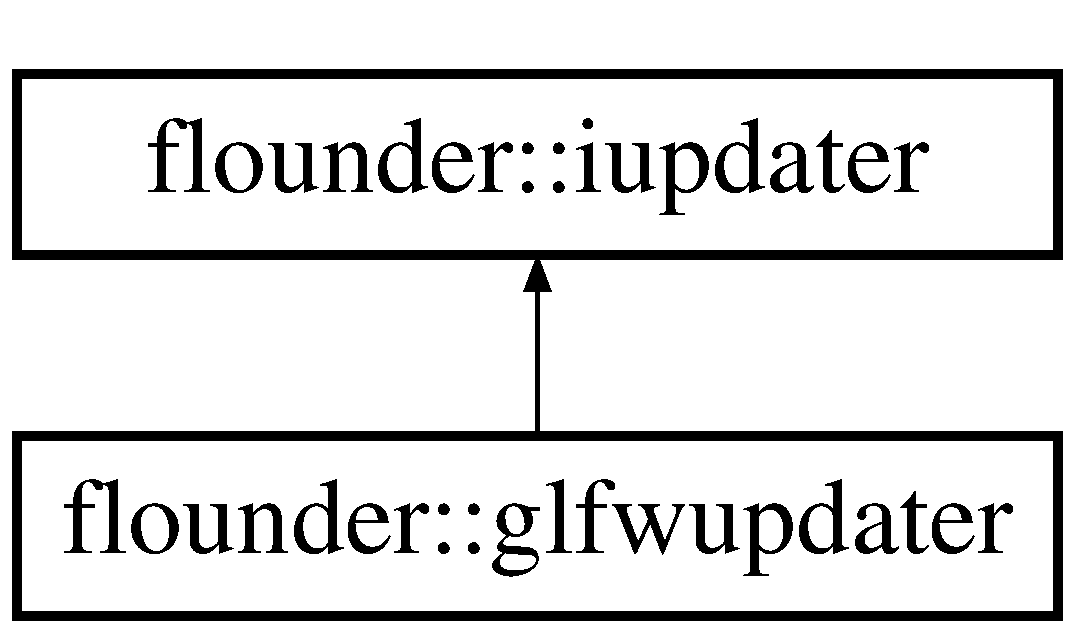
\includegraphics[height=2.000000cm]{classflounder_1_1glfwupdater}
\end{center}
\end{figure}
\subsection*{Public Member Functions}
\begin{DoxyCompactItemize}
\item 
\mbox{\Hypertarget{classflounder_1_1glfwupdater_acd58077965d5ba137961c567d7d79aa9}\label{classflounder_1_1glfwupdater_acd58077965d5ba137961c567d7d79aa9}} 
void {\bfseries create} () override
\item 
\mbox{\Hypertarget{classflounder_1_1glfwupdater_ab0c8addaf2393f4c88969e71ed78f600}\label{classflounder_1_1glfwupdater_ab0c8addaf2393f4c88969e71ed78f600}} 
void {\bfseries init} () override
\item 
\mbox{\Hypertarget{classflounder_1_1glfwupdater_a2443d270f702e67ab44c7afb88c71a5e}\label{classflounder_1_1glfwupdater_a2443d270f702e67ab44c7afb88c71a5e}} 
void {\bfseries update} () override
\item 
\hyperlink{classflounder_1_1imodule}{imodule} $\ast$ \hyperlink{classflounder_1_1glfwupdater_a284945635b93ffc1bd6164ff20565349}{get\+Instance} (const std\+::string \&name) override
\begin{DoxyCompactList}\small\item\em Gets a module from the updater. \end{DoxyCompactList}\item 
double \hyperlink{classflounder_1_1glfwupdater_a6393f60d2b0f84a78ccf14b0c55ae1ee}{get\+Time\+Offset} () override
\begin{DoxyCompactList}\small\item\em Gets the added/removed time for the framework (seconds). \end{DoxyCompactList}\item 
void \hyperlink{classflounder_1_1glfwupdater_a7dc4371863e39a3a7870e4a2ac539fed}{set\+Time\+Offset} (const double \&time\+Offset) override
\begin{DoxyCompactList}\small\item\em Sets the time offset for the framework (seconds). \end{DoxyCompactList}\item 
double \hyperlink{classflounder_1_1glfwupdater_a8da4916f3335126413a072203b94a735}{get\+Delta} () override
\begin{DoxyCompactList}\small\item\em Gets the delta (seconds) between updates. \end{DoxyCompactList}\item 
double \hyperlink{classflounder_1_1glfwupdater_a3f8d8a108c8db0d2ead35088646687c9}{get\+Delta\+Render} () override
\begin{DoxyCompactList}\small\item\em Gets the delta (seconds) between renders. \end{DoxyCompactList}\item 
double \hyperlink{classflounder_1_1glfwupdater_a6982b83970693347bfa460adc04cf984}{get\+Time\+Sec} () override
\begin{DoxyCompactList}\small\item\em Gets the current time of the framework instance. \end{DoxyCompactList}\item 
double \hyperlink{classflounder_1_1glfwupdater_a1c3b884efb6e785143db556d4db9bdc8}{get\+Time\+Ms} () override
\begin{DoxyCompactList}\small\item\em Gets the current time of the framework instance. \end{DoxyCompactList}\end{DoxyCompactItemize}
\subsection*{Private Attributes}
\begin{DoxyCompactItemize}
\item 
\mbox{\Hypertarget{classflounder_1_1glfwupdater_a7a183f7c8b615547222348cfc727c138}\label{classflounder_1_1glfwupdater_a7a183f7c8b615547222348cfc727c138}} 
double {\bfseries m\+\_\+start\+Time}
\item 
\mbox{\Hypertarget{classflounder_1_1glfwupdater_aecb7f675d1aa26d04f0933768d7b8189}\label{classflounder_1_1glfwupdater_aecb7f675d1aa26d04f0933768d7b8189}} 
double {\bfseries m\+\_\+time\+Offset}
\item 
\mbox{\Hypertarget{classflounder_1_1glfwupdater_ab9cbfc326d5541b950cd1bb2b4e777ee}\label{classflounder_1_1glfwupdater_ab9cbfc326d5541b950cd1bb2b4e777ee}} 
\hyperlink{classflounder_1_1delta}{delta} $\ast$ {\bfseries m\+\_\+delta\+Update}
\item 
\mbox{\Hypertarget{classflounder_1_1glfwupdater_a77590ce7ebb3f3aa8b69e95e2ae98fb4}\label{classflounder_1_1glfwupdater_a77590ce7ebb3f3aa8b69e95e2ae98fb4}} 
\hyperlink{classflounder_1_1delta}{delta} $\ast$ {\bfseries m\+\_\+delta\+Render}
\item 
\mbox{\Hypertarget{classflounder_1_1glfwupdater_ab00958332ab500ed7e52bd74ae01c2c9}\label{classflounder_1_1glfwupdater_ab00958332ab500ed7e52bd74ae01c2c9}} 
\hyperlink{classflounder_1_1timer}{timer} $\ast$ {\bfseries m\+\_\+timer\+Update}
\item 
\mbox{\Hypertarget{classflounder_1_1glfwupdater_ac3dae6d2a82d58c796a2c095a928e897}\label{classflounder_1_1glfwupdater_ac3dae6d2a82d58c796a2c095a928e897}} 
\hyperlink{classflounder_1_1timer}{timer} $\ast$ {\bfseries m\+\_\+timer\+Render}
\item 
\mbox{\Hypertarget{classflounder_1_1glfwupdater_a053b12c63465fc37424420bc55d00e79}\label{classflounder_1_1glfwupdater_a053b12c63465fc37424420bc55d00e79}} 
\hyperlink{classflounder_1_1timer}{timer} $\ast$ {\bfseries m\+\_\+timer\+Log}
\item 
\mbox{\Hypertarget{classflounder_1_1glfwupdater_a91275f1c4dbdd6035d3199ad0bb9e70f}\label{classflounder_1_1glfwupdater_a91275f1c4dbdd6035d3199ad0bb9e70f}} 
\hyperlink{classflounder_1_1events}{events} $\ast$ {\bfseries m\+\_\+events}
\item 
\mbox{\Hypertarget{classflounder_1_1glfwupdater_a02670cabb35d9ad5f800900d05afcdc9}\label{classflounder_1_1glfwupdater_a02670cabb35d9ad5f800900d05afcdc9}} 
\hyperlink{classflounder_1_1tasks}{tasks} $\ast$ {\bfseries m\+\_\+tasks}
\item 
\mbox{\Hypertarget{classflounder_1_1glfwupdater_ac8bb3d6684a216d8216505c5798b192d}\label{classflounder_1_1glfwupdater_ac8bb3d6684a216d8216505c5798b192d}} 
\hyperlink{classflounder_1_1processing}{processing} $\ast$ {\bfseries m\+\_\+processing}
\item 
\mbox{\Hypertarget{classflounder_1_1glfwupdater_a91464cfb83ec6cabf02c2ad8831b8496}\label{classflounder_1_1glfwupdater_a91464cfb83ec6cabf02c2ad8831b8496}} 
\hyperlink{classflounder_1_1display}{display} $\ast$ {\bfseries m\+\_\+display}
\item 
\mbox{\Hypertarget{classflounder_1_1glfwupdater_a1380d5789c482cb0083ab38e4091c338}\label{classflounder_1_1glfwupdater_a1380d5789c482cb0083ab38e4091c338}} 
\hyperlink{classflounder_1_1joysticks}{joysticks} $\ast$ {\bfseries m\+\_\+joysticks}
\item 
\mbox{\Hypertarget{classflounder_1_1glfwupdater_aae51a3d0e5bfc126ef1bb4f4a7d4a6bc}\label{classflounder_1_1glfwupdater_aae51a3d0e5bfc126ef1bb4f4a7d4a6bc}} 
\hyperlink{classflounder_1_1keyboard}{keyboard} $\ast$ {\bfseries m\+\_\+keyboard}
\item 
\mbox{\Hypertarget{classflounder_1_1glfwupdater_a45bb27f3ef7b383920d838c445576596}\label{classflounder_1_1glfwupdater_a45bb27f3ef7b383920d838c445576596}} 
\hyperlink{classflounder_1_1mouse}{mouse} $\ast$ {\bfseries m\+\_\+mouse}
\item 
\mbox{\Hypertarget{classflounder_1_1glfwupdater_a41a21fd6ad15b9ccf061a60d81dbd9ee}\label{classflounder_1_1glfwupdater_a41a21fd6ad15b9ccf061a60d81dbd9ee}} 
\hyperlink{classflounder_1_1audio}{audio} $\ast$ {\bfseries m\+\_\+audio}
\item 
\mbox{\Hypertarget{classflounder_1_1glfwupdater_a519e22699793fc11ba9e14862871d1dc}\label{classflounder_1_1glfwupdater_a519e22699793fc11ba9e14862871d1dc}} 
\hyperlink{classflounder_1_1standards}{standards} $\ast$ {\bfseries m\+\_\+standards}
\item 
\mbox{\Hypertarget{classflounder_1_1glfwupdater_ac315975083fe903f32835f3ec74afc7b}\label{classflounder_1_1glfwupdater_ac315975083fe903f32835f3ec74afc7b}} 
\hyperlink{classflounder_1_1camera}{camera} $\ast$ {\bfseries m\+\_\+camera}
\item 
\mbox{\Hypertarget{classflounder_1_1glfwupdater_a64e02877af0738b122d5e6b62fb33444}\label{classflounder_1_1glfwupdater_a64e02877af0738b122d5e6b62fb33444}} 
\hyperlink{classflounder_1_1loaders}{loaders} $\ast$ {\bfseries m\+\_\+loaders}
\item 
\mbox{\Hypertarget{classflounder_1_1glfwupdater_a158be0a69d98920683673fd0b5253a8a}\label{classflounder_1_1glfwupdater_a158be0a69d98920683673fd0b5253a8a}} 
renderer $\ast$ {\bfseries m\+\_\+renderer}
\item 
\mbox{\Hypertarget{classflounder_1_1glfwupdater_a122cce841e350d3c4a9214b8a91918fa}\label{classflounder_1_1glfwupdater_a122cce841e350d3c4a9214b8a91918fa}} 
\hyperlink{classflounder_1_1skybox}{skybox} $\ast$ {\bfseries m\+\_\+skybox}
\end{DoxyCompactItemize}


\subsection{Detailed Description}
The default G\+L\+FW updater for the framework. 



\subsection{Member Function Documentation}
\mbox{\Hypertarget{classflounder_1_1glfwupdater_a8da4916f3335126413a072203b94a735}\label{classflounder_1_1glfwupdater_a8da4916f3335126413a072203b94a735}} 
\index{flounder\+::glfwupdater@{flounder\+::glfwupdater}!get\+Delta@{get\+Delta}}
\index{get\+Delta@{get\+Delta}!flounder\+::glfwupdater@{flounder\+::glfwupdater}}
\subsubsection{\texorpdfstring{get\+Delta()}{getDelta()}}
{\footnotesize\ttfamily double flounder\+::glfwupdater\+::get\+Delta (\begin{DoxyParamCaption}{ }\end{DoxyParamCaption})\hspace{0.3cm}{\ttfamily [inline]}, {\ttfamily [override]}, {\ttfamily [virtual]}}



Gets the delta (seconds) between updates. 

\begin{DoxyReturn}{Returns}
The delta between updates. 
\end{DoxyReturn}


Implements \hyperlink{classflounder_1_1iupdater_a1e8d40602f9799fc82d96d5b845cf796}{flounder\+::iupdater}.

\mbox{\Hypertarget{classflounder_1_1glfwupdater_a3f8d8a108c8db0d2ead35088646687c9}\label{classflounder_1_1glfwupdater_a3f8d8a108c8db0d2ead35088646687c9}} 
\index{flounder\+::glfwupdater@{flounder\+::glfwupdater}!get\+Delta\+Render@{get\+Delta\+Render}}
\index{get\+Delta\+Render@{get\+Delta\+Render}!flounder\+::glfwupdater@{flounder\+::glfwupdater}}
\subsubsection{\texorpdfstring{get\+Delta\+Render()}{getDeltaRender()}}
{\footnotesize\ttfamily double flounder\+::glfwupdater\+::get\+Delta\+Render (\begin{DoxyParamCaption}{ }\end{DoxyParamCaption})\hspace{0.3cm}{\ttfamily [inline]}, {\ttfamily [override]}, {\ttfamily [virtual]}}



Gets the delta (seconds) between renders. 

\begin{DoxyReturn}{Returns}
The delta between renders. 
\end{DoxyReturn}


Implements \hyperlink{classflounder_1_1iupdater_a00d7cf530cfbd7f83c8903328da14027}{flounder\+::iupdater}.

\mbox{\Hypertarget{classflounder_1_1glfwupdater_a284945635b93ffc1bd6164ff20565349}\label{classflounder_1_1glfwupdater_a284945635b93ffc1bd6164ff20565349}} 
\index{flounder\+::glfwupdater@{flounder\+::glfwupdater}!get\+Instance@{get\+Instance}}
\index{get\+Instance@{get\+Instance}!flounder\+::glfwupdater@{flounder\+::glfwupdater}}
\subsubsection{\texorpdfstring{get\+Instance()}{getInstance()}}
{\footnotesize\ttfamily \hyperlink{classflounder_1_1imodule}{imodule} $\ast$ flounder\+::glfwupdater\+::get\+Instance (\begin{DoxyParamCaption}\item[{const std\+::string \&}]{name }\end{DoxyParamCaption})\hspace{0.3cm}{\ttfamily [override]}, {\ttfamily [virtual]}}



Gets a module from the updater. 


\begin{DoxyParams}{Parameters}
{\em key} & The module name/key to get. \\
\hline
\end{DoxyParams}
\begin{DoxyReturn}{Returns}
The module object. 
\end{DoxyReturn}


Implements \hyperlink{classflounder_1_1iupdater_a391b1788b5c139b199ed48033da1b88d}{flounder\+::iupdater}.

\mbox{\Hypertarget{classflounder_1_1glfwupdater_a1c3b884efb6e785143db556d4db9bdc8}\label{classflounder_1_1glfwupdater_a1c3b884efb6e785143db556d4db9bdc8}} 
\index{flounder\+::glfwupdater@{flounder\+::glfwupdater}!get\+Time\+Ms@{get\+Time\+Ms}}
\index{get\+Time\+Ms@{get\+Time\+Ms}!flounder\+::glfwupdater@{flounder\+::glfwupdater}}
\subsubsection{\texorpdfstring{get\+Time\+Ms()}{getTimeMs()}}
{\footnotesize\ttfamily double flounder\+::glfwupdater\+::get\+Time\+Ms (\begin{DoxyParamCaption}{ }\end{DoxyParamCaption})\hspace{0.3cm}{\ttfamily [inline]}, {\ttfamily [override]}, {\ttfamily [virtual]}}



Gets the current time of the framework instance. 

\begin{DoxyReturn}{Returns}
The current framework time in milliseconds. 
\end{DoxyReturn}


Implements \hyperlink{classflounder_1_1iupdater_a56548faad88ad85e0cb4bc96af0912d6}{flounder\+::iupdater}.

\mbox{\Hypertarget{classflounder_1_1glfwupdater_a6393f60d2b0f84a78ccf14b0c55ae1ee}\label{classflounder_1_1glfwupdater_a6393f60d2b0f84a78ccf14b0c55ae1ee}} 
\index{flounder\+::glfwupdater@{flounder\+::glfwupdater}!get\+Time\+Offset@{get\+Time\+Offset}}
\index{get\+Time\+Offset@{get\+Time\+Offset}!flounder\+::glfwupdater@{flounder\+::glfwupdater}}
\subsubsection{\texorpdfstring{get\+Time\+Offset()}{getTimeOffset()}}
{\footnotesize\ttfamily double flounder\+::glfwupdater\+::get\+Time\+Offset (\begin{DoxyParamCaption}{ }\end{DoxyParamCaption})\hspace{0.3cm}{\ttfamily [inline]}, {\ttfamily [override]}, {\ttfamily [virtual]}}



Gets the added/removed time for the framework (seconds). 

\begin{DoxyReturn}{Returns}
The time offset. 
\end{DoxyReturn}


Implements \hyperlink{classflounder_1_1iupdater_abd983cbbeed27f28e9be768a2d3b69f2}{flounder\+::iupdater}.

\mbox{\Hypertarget{classflounder_1_1glfwupdater_a6982b83970693347bfa460adc04cf984}\label{classflounder_1_1glfwupdater_a6982b83970693347bfa460adc04cf984}} 
\index{flounder\+::glfwupdater@{flounder\+::glfwupdater}!get\+Time\+Sec@{get\+Time\+Sec}}
\index{get\+Time\+Sec@{get\+Time\+Sec}!flounder\+::glfwupdater@{flounder\+::glfwupdater}}
\subsubsection{\texorpdfstring{get\+Time\+Sec()}{getTimeSec()}}
{\footnotesize\ttfamily double flounder\+::glfwupdater\+::get\+Time\+Sec (\begin{DoxyParamCaption}{ }\end{DoxyParamCaption})\hspace{0.3cm}{\ttfamily [inline]}, {\ttfamily [override]}, {\ttfamily [virtual]}}



Gets the current time of the framework instance. 

\begin{DoxyReturn}{Returns}
The current framework time in seconds. 
\end{DoxyReturn}


Implements \hyperlink{classflounder_1_1iupdater_a071086b844e1f90d7f3577e80c9c09fe}{flounder\+::iupdater}.

\mbox{\Hypertarget{classflounder_1_1glfwupdater_a7dc4371863e39a3a7870e4a2ac539fed}\label{classflounder_1_1glfwupdater_a7dc4371863e39a3a7870e4a2ac539fed}} 
\index{flounder\+::glfwupdater@{flounder\+::glfwupdater}!set\+Time\+Offset@{set\+Time\+Offset}}
\index{set\+Time\+Offset@{set\+Time\+Offset}!flounder\+::glfwupdater@{flounder\+::glfwupdater}}
\subsubsection{\texorpdfstring{set\+Time\+Offset()}{setTimeOffset()}}
{\footnotesize\ttfamily void flounder\+::glfwupdater\+::set\+Time\+Offset (\begin{DoxyParamCaption}\item[{const double \&}]{time\+Offset }\end{DoxyParamCaption})\hspace{0.3cm}{\ttfamily [inline]}, {\ttfamily [override]}, {\ttfamily [virtual]}}



Sets the time offset for the framework (seconds). 


\begin{DoxyParams}{Parameters}
{\em time\+Offset} & The new time offset. \\
\hline
\end{DoxyParams}


Implements \hyperlink{classflounder_1_1iupdater_aa6aa143e40a5a39bcd53753798438ea1}{flounder\+::iupdater}.



The documentation for this class was generated from the following files\+:\begin{DoxyCompactItemize}
\item 
Flounder-\/\+Core/src/framework/glfw/glfwupdater.\+h\item 
Flounder-\/\+Core/src/framework/glfw/glfwupdater.\+cpp\end{DoxyCompactItemize}

\hypertarget{classflounder_1_1grabberjoystick}{}\section{flounder\+:\+:grabberjoystick Class Reference}
\label{classflounder_1_1grabberjoystick}\index{flounder\+::grabberjoystick@{flounder\+::grabberjoystick}}
Inheritance diagram for flounder\+:\+:grabberjoystick\+:\begin{figure}[H]
\begin{center}
\leavevmode
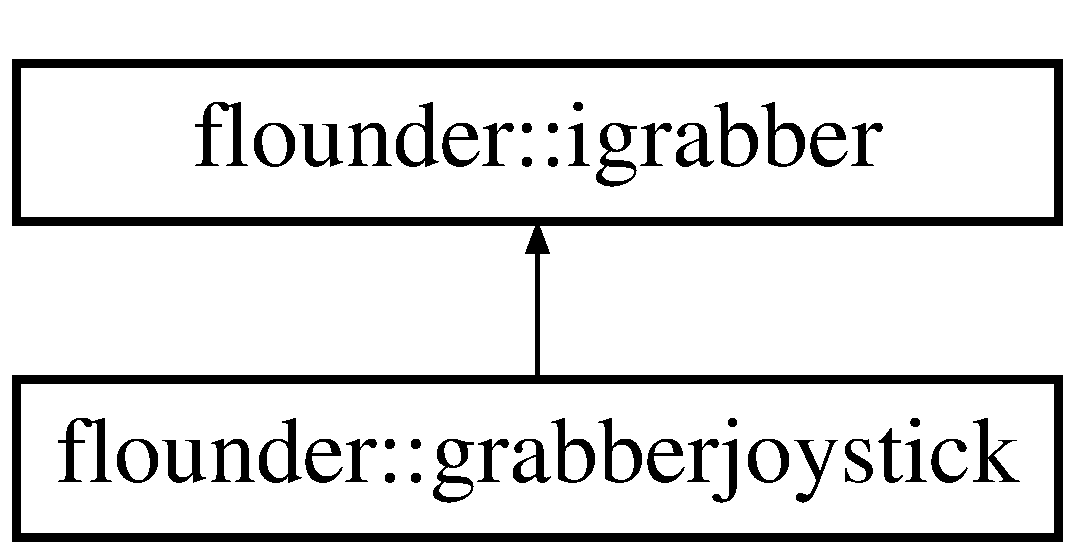
\includegraphics[height=2.000000cm]{classflounder_1_1grabberjoystick}
\end{center}
\end{figure}
\subsection*{Public Member Functions}
\begin{DoxyCompactItemize}
\item 
\mbox{\Hypertarget{classflounder_1_1grabberjoystick_a6dedf47e19d77f14d1bcd4f3544ed10a}\label{classflounder_1_1grabberjoystick_a6dedf47e19d77f14d1bcd4f3544ed10a}} 
{\bfseries grabberjoystick} (const int \&joystick)
\item 
\mbox{\Hypertarget{classflounder_1_1grabberjoystick_ad2755c3e80f83cf63124add2571f194c}\label{classflounder_1_1grabberjoystick_ad2755c3e80f83cf63124add2571f194c}} 
int {\bfseries get\+Current} (\hyperlink{classflounder_1_1text}{text} $\ast$object) override
\item 
\mbox{\Hypertarget{classflounder_1_1grabberjoystick_a17d03c76fcdec47283904d63cbd8b9f5}\label{classflounder_1_1grabberjoystick_a17d03c76fcdec47283904d63cbd8b9f5}} 
std\+::string {\bfseries get\+Value} (const int \&value) override
\end{DoxyCompactItemize}
\subsection*{Private Attributes}
\begin{DoxyCompactItemize}
\item 
\mbox{\Hypertarget{classflounder_1_1grabberjoystick_a1e41b76d6df5ecf30081747048aa76bf}\label{classflounder_1_1grabberjoystick_a1e41b76d6df5ecf30081747048aa76bf}} 
int {\bfseries m\+\_\+joystick}
\end{DoxyCompactItemize}


The documentation for this class was generated from the following files\+:\begin{DoxyCompactItemize}
\item 
Flounder-\/\+Core/src/uis/inputgrabber.\+h\item 
Flounder-\/\+Core/src/uis/inputgrabber.\+cpp\end{DoxyCompactItemize}

\hypertarget{classflounder_1_1grabberkeyboard}{}\section{flounder\+:\+:grabberkeyboard Class Reference}
\label{classflounder_1_1grabberkeyboard}\index{flounder\+::grabberkeyboard@{flounder\+::grabberkeyboard}}
Inheritance diagram for flounder\+:\+:grabberkeyboard\+:\begin{figure}[H]
\begin{center}
\leavevmode
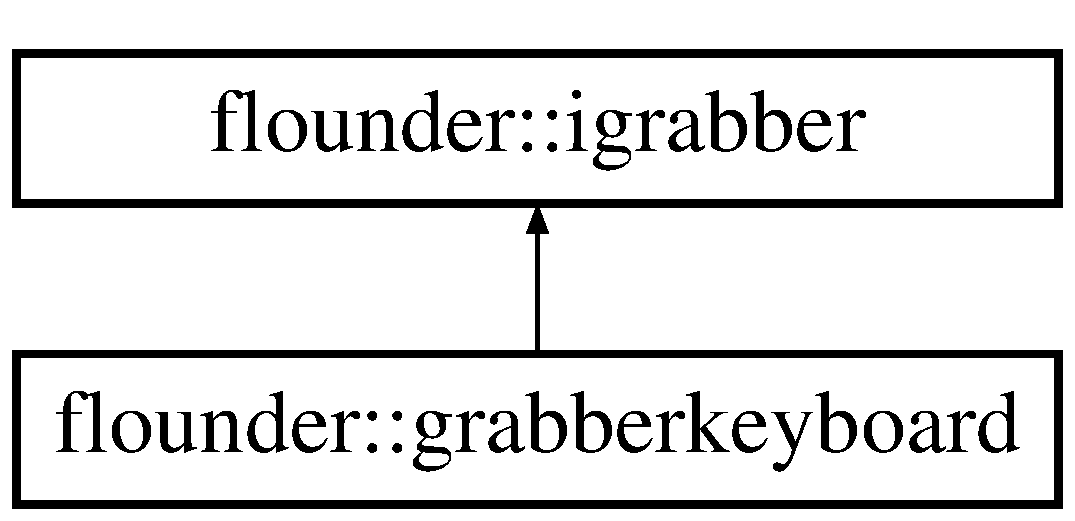
\includegraphics[height=2.000000cm]{classflounder_1_1grabberkeyboard}
\end{center}
\end{figure}
\subsection*{Public Member Functions}
\begin{DoxyCompactItemize}
\item 
\mbox{\Hypertarget{classflounder_1_1grabberkeyboard_a5b60f06cd5a18cd8b66888c6796064a2}\label{classflounder_1_1grabberkeyboard_a5b60f06cd5a18cd8b66888c6796064a2}} 
int {\bfseries get\+Current} (\hyperlink{classflounder_1_1text}{text} $\ast$object) override
\item 
\mbox{\Hypertarget{classflounder_1_1grabberkeyboard_ae45f2c235bbca57be99b9e571aeae176}\label{classflounder_1_1grabberkeyboard_ae45f2c235bbca57be99b9e571aeae176}} 
std\+::string {\bfseries get\+Value} (const int \&value) override
\end{DoxyCompactItemize}


The documentation for this class was generated from the following files\+:\begin{DoxyCompactItemize}
\item 
Flounder-\/\+Core/src/uis/inputgrabber.\+h\item 
Flounder-\/\+Core/src/uis/inputgrabber.\+cpp\end{DoxyCompactItemize}

\hypertarget{classflounder_1_1grabbermouse}{}\section{flounder\+:\+:grabbermouse Class Reference}
\label{classflounder_1_1grabbermouse}\index{flounder\+::grabbermouse@{flounder\+::grabbermouse}}
Inheritance diagram for flounder\+:\+:grabbermouse\+:\begin{figure}[H]
\begin{center}
\leavevmode
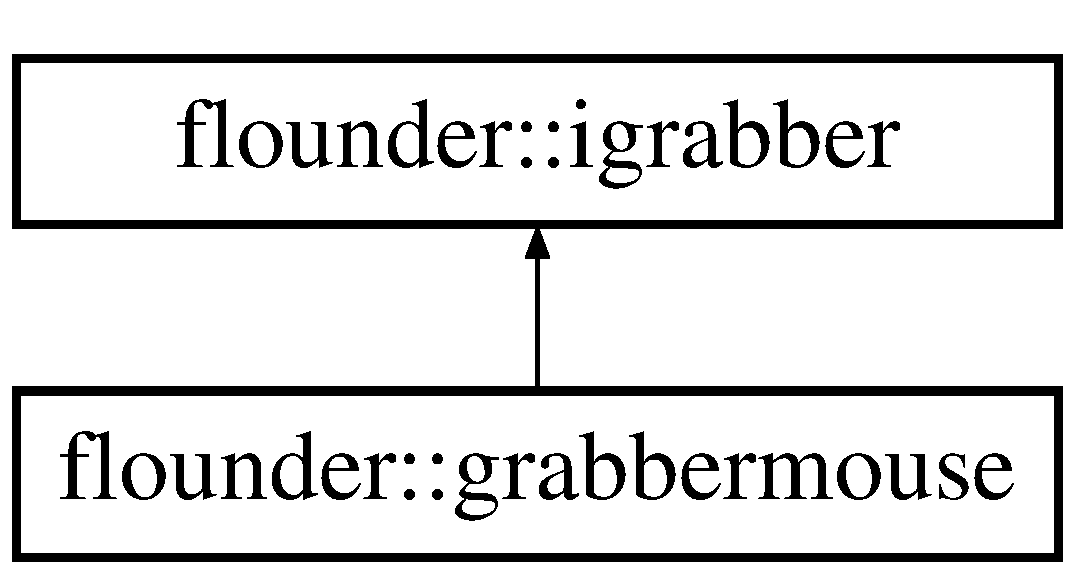
\includegraphics[height=2.000000cm]{classflounder_1_1grabbermouse}
\end{center}
\end{figure}
\subsection*{Public Member Functions}
\begin{DoxyCompactItemize}
\item 
\mbox{\Hypertarget{classflounder_1_1grabbermouse_a6c5ea248350f50c805ede82b2f7b307d}\label{classflounder_1_1grabbermouse_a6c5ea248350f50c805ede82b2f7b307d}} 
int {\bfseries get\+Current} (\hyperlink{classflounder_1_1text}{text} $\ast$object) override
\item 
\mbox{\Hypertarget{classflounder_1_1grabbermouse_a630d39a6efe37372abd012b7dda0f698}\label{classflounder_1_1grabbermouse_a630d39a6efe37372abd012b7dda0f698}} 
std\+::string {\bfseries get\+Value} (const int \&value) override
\end{DoxyCompactItemize}


The documentation for this class was generated from the following files\+:\begin{DoxyCompactItemize}
\item 
Flounder-\/\+Core/src/uis/inputgrabber.\+h\item 
Flounder-\/\+Core/src/uis/inputgrabber.\+cpp\end{DoxyCompactItemize}

\hypertarget{classflounder_1_1gui}{}\section{flounder\+:\+:gui Class Reference}
\label{classflounder_1_1gui}\index{flounder\+::gui@{flounder\+::gui}}


A object the represents a texture in a G\+UI.  




{\ttfamily \#include $<$gui.\+h$>$}

Inheritance diagram for flounder\+:\+:gui\+:\begin{figure}[H]
\begin{center}
\leavevmode
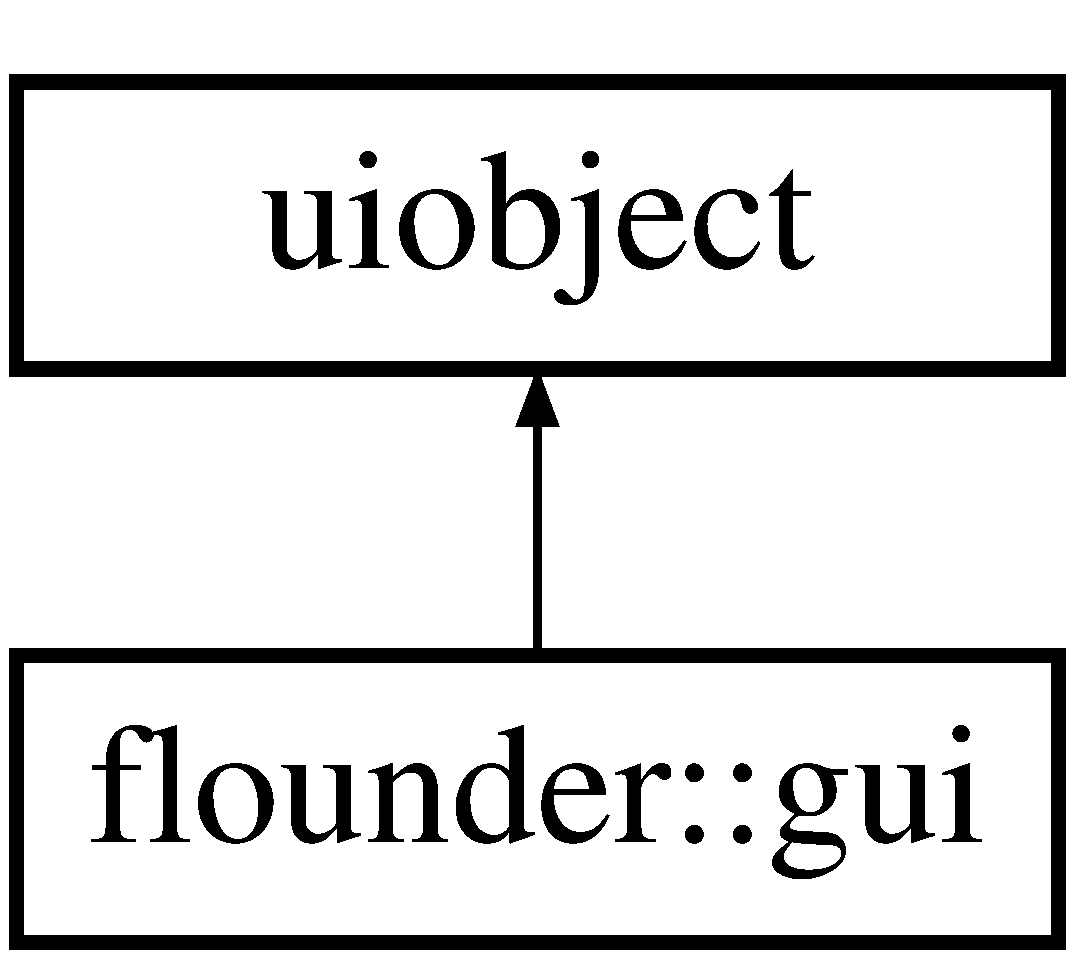
\includegraphics[height=2.000000cm]{classflounder_1_1gui}
\end{center}
\end{figure}
\subsection*{Public Member Functions}
\begin{DoxyCompactItemize}
\item 
\hyperlink{classflounder_1_1gui_a95658ab4bcf45269d6d0c852a913c85d}{gui} (uiobject $\ast$parent, const \hyperlink{classflounder_1_1vector2}{vector2} \&position, const \hyperlink{classflounder_1_1vector2}{vector2} \&dimensions, \hyperlink{classflounder_1_1texture}{texture} $\ast$\hyperlink{classflounder_1_1texture}{texture}, const int \&selected\+Row)
\begin{DoxyCompactList}\small\item\em Creates a new G\+UI object. \end{DoxyCompactList}\item 
\hyperlink{classflounder_1_1gui_ab956f28a5e730f928a48490255346787}{$\sim$gui} ()
\begin{DoxyCompactList}\small\item\em Deconstructor for the gui object. \end{DoxyCompactList}\item 
\mbox{\Hypertarget{classflounder_1_1gui_a4ab9fe21b6a34200aa8b79b0008332b2}\label{classflounder_1_1gui_a4ab9fe21b6a34200aa8b79b0008332b2}} 
void {\bfseries update\+Object} () override
\item 
\mbox{\Hypertarget{classflounder_1_1gui_afadb039858588ff99dd4d236d22833ab}\label{classflounder_1_1gui_afadb039858588ff99dd4d236d22833ab}} 
\hyperlink{classflounder_1_1texture}{texture} $\ast$ {\bfseries get\+Texture} ()
\item 
\mbox{\Hypertarget{classflounder_1_1gui_acb02288e8176c842ffdb0123561d993d}\label{classflounder_1_1gui_acb02288e8176c842ffdb0123561d993d}} 
void {\bfseries set\+Texture} (\hyperlink{classflounder_1_1texture}{texture} $\ast$\hyperlink{classflounder_1_1texture}{texture})
\item 
\mbox{\Hypertarget{classflounder_1_1gui_ad767ee1ea49f217abce7533973d862a9}\label{classflounder_1_1gui_ad767ee1ea49f217abce7533973d862a9}} 
bool {\bfseries get\+Flip\+Texture} ()
\item 
\mbox{\Hypertarget{classflounder_1_1gui_a0099ff0cbb0e3c9a4b227160043f1fc3}\label{classflounder_1_1gui_a0099ff0cbb0e3c9a4b227160043f1fc3}} 
void {\bfseries set\+Flip\+Texture} (const bool \&flip\+Texture)
\item 
\mbox{\Hypertarget{classflounder_1_1gui_a09e7d3428923dd2c6b1f71d6275c3b2c}\label{classflounder_1_1gui_a09e7d3428923dd2c6b1f71d6275c3b2c}} 
int {\bfseries get\+Selected\+Row} ()
\item 
\mbox{\Hypertarget{classflounder_1_1gui_a27cea6ffb465a8de4cbdfbd69ad2df4e}\label{classflounder_1_1gui_a27cea6ffb465a8de4cbdfbd69ad2df4e}} 
void {\bfseries set\+Selected\+Row} (const int \&selected\+Row)
\item 
\mbox{\Hypertarget{classflounder_1_1gui_a7daf537514e6bfb3155a8f63350971e5}\label{classflounder_1_1gui_a7daf537514e6bfb3155a8f63350971e5}} 
\hyperlink{classflounder_1_1vector2}{vector2} $\ast$ {\bfseries get\+Texture\+Offset} ()
\item 
\mbox{\Hypertarget{classflounder_1_1gui_a850b142bfe51d61f2b4c1dc3676bc2e5}\label{classflounder_1_1gui_a850b142bfe51d61f2b4c1dc3676bc2e5}} 
void {\bfseries set\+Texture\+Offset} (const \hyperlink{classflounder_1_1vector2}{vector2} \&texture\+Offset)
\item 
\mbox{\Hypertarget{classflounder_1_1gui_afcc8ae6ea69dc4b23c672895a476e595}\label{classflounder_1_1gui_afcc8ae6ea69dc4b23c672895a476e595}} 
\hyperlink{classflounder_1_1colour}{colour} $\ast$ {\bfseries get\+Colour\+Offset} ()
\item 
\mbox{\Hypertarget{classflounder_1_1gui_a220cfc75d2d7bb565fbb37d954b08f06}\label{classflounder_1_1gui_a220cfc75d2d7bb565fbb37d954b08f06}} 
void {\bfseries set\+Colour\+Offset} (const \hyperlink{classflounder_1_1colour}{colour} \&colour\+Offset)
\end{DoxyCompactItemize}
\subsection*{Private Attributes}
\begin{DoxyCompactItemize}
\item 
\mbox{\Hypertarget{classflounder_1_1gui_a79436b6b873a5fc6b0c539242b1ee98d}\label{classflounder_1_1gui_a79436b6b873a5fc6b0c539242b1ee98d}} 
\hyperlink{classflounder_1_1texture}{texture} $\ast$ {\bfseries m\+\_\+texture}
\item 
\mbox{\Hypertarget{classflounder_1_1gui_a3ff46ec0f4992a6b0b0099b02a1a20d3}\label{classflounder_1_1gui_a3ff46ec0f4992a6b0b0099b02a1a20d3}} 
bool {\bfseries m\+\_\+flip\+Texture}
\item 
\mbox{\Hypertarget{classflounder_1_1gui_a9574dbb0684eb23cc000707188f1922d}\label{classflounder_1_1gui_a9574dbb0684eb23cc000707188f1922d}} 
int {\bfseries m\+\_\+selected\+Row}
\item 
\mbox{\Hypertarget{classflounder_1_1gui_aa7281add10d424b2c44571a549857dbc}\label{classflounder_1_1gui_aa7281add10d424b2c44571a549857dbc}} 
\hyperlink{classflounder_1_1vector2}{vector2} $\ast$ {\bfseries m\+\_\+texture\+Offset}
\item 
\mbox{\Hypertarget{classflounder_1_1gui_a075aab9ab9b066143ccce77cd6dca6dd}\label{classflounder_1_1gui_a075aab9ab9b066143ccce77cd6dca6dd}} 
\hyperlink{classflounder_1_1colour}{colour} $\ast$ {\bfseries m\+\_\+colour\+Offset}
\end{DoxyCompactItemize}


\subsection{Detailed Description}
A object the represents a texture in a G\+UI. 



\subsection{Constructor \& Destructor Documentation}
\mbox{\Hypertarget{classflounder_1_1gui_a95658ab4bcf45269d6d0c852a913c85d}\label{classflounder_1_1gui_a95658ab4bcf45269d6d0c852a913c85d}} 
\index{flounder\+::gui@{flounder\+::gui}!gui@{gui}}
\index{gui@{gui}!flounder\+::gui@{flounder\+::gui}}
\subsubsection{\texorpdfstring{gui()}{gui()}}
{\footnotesize\ttfamily flounder\+::gui\+::gui (\begin{DoxyParamCaption}\item[{uiobject $\ast$}]{parent,  }\item[{const \hyperlink{classflounder_1_1vector2}{vector2} \&}]{position,  }\item[{const \hyperlink{classflounder_1_1vector2}{vector2} \&}]{dimensions,  }\item[{\hyperlink{classflounder_1_1texture}{texture} $\ast$}]{texture,  }\item[{const int \&}]{selected\+Row }\end{DoxyParamCaption})}



Creates a new G\+UI object. 


\begin{DoxyParams}{Parameters}
{\em parent} & The objects parent. \\
\hline
{\em position} & The objects position relative to the parents. \\
\hline
{\em dimensions} & The objects dimensions. \\
\hline
{\em texture} & The objects texture. \\
\hline
{\em selected\+Row} & The default row of the texture to render from. \\
\hline
\end{DoxyParams}
\mbox{\Hypertarget{classflounder_1_1gui_ab956f28a5e730f928a48490255346787}\label{classflounder_1_1gui_ab956f28a5e730f928a48490255346787}} 
\index{flounder\+::gui@{flounder\+::gui}!````~gui@{$\sim$gui}}
\index{````~gui@{$\sim$gui}!flounder\+::gui@{flounder\+::gui}}
\subsubsection{\texorpdfstring{$\sim$gui()}{~gui()}}
{\footnotesize\ttfamily flounder\+::gui\+::$\sim$gui (\begin{DoxyParamCaption}{ }\end{DoxyParamCaption})}



Deconstructor for the gui object. 



The documentation for this class was generated from the following files\+:\begin{DoxyCompactItemize}
\item 
Flounder-\/\+Core/src/guis/gui.\+h\item 
Flounder-\/\+Core/src/guis/gui.\+cpp\end{DoxyCompactItemize}

\hypertarget{classflounder_1_1helperarray}{}\section{flounder\+:\+:helperarray Class Reference}
\label{classflounder_1_1helperarray}\index{flounder\+::helperarray@{flounder\+::helperarray}}
\subsection*{Static Public Member Functions}
\begin{DoxyCompactItemize}
\item 
\mbox{\Hypertarget{classflounder_1_1helperarray_a0a0bb008d5879a1f43eb87efbc30971b}\label{classflounder_1_1helperarray_a0a0bb008d5879a1f43eb87efbc30971b}} 
static float $\ast$$\ast$ {\bfseries rec\+Float\+Array} (const int \&size1, const int \&size2)
\end{DoxyCompactItemize}


The documentation for this class was generated from the following file\+:\begin{DoxyCompactItemize}
\item 
C\+:/\+Users/mattp/\+Documents/\+Flounder/\+Flounder\+Core/\+Sources/helpers/helperarray.\+h\end{DoxyCompactItemize}

\hypertarget{classflounder_1_1helperfile}{}\section{flounder\+:\+:helperfile Class Reference}
\label{classflounder_1_1helperfile}\index{flounder\+::helperfile@{flounder\+::helperfile}}
\subsection*{Static Public Member Functions}
\begin{DoxyCompactItemize}
\item 
\mbox{\Hypertarget{classflounder_1_1helperfile_a3e0cf9aeb402172757a2ee2bf22a4c7f}\label{classflounder_1_1helperfile_a3e0cf9aeb402172757a2ee2bf22a4c7f}} 
static std\+::string {\bfseries read\+File} (const std\+::string \&filepath)
\end{DoxyCompactItemize}


The documentation for this class was generated from the following file\+:\begin{DoxyCompactItemize}
\item 
C\+:/\+Users/mattp/\+Documents/\+Flounder/\+Flounder\+Core/\+Sources/helpers/helperfile.\+h\end{DoxyCompactItemize}

\hypertarget{classflounder_1_1helperstring}{}\section{flounder\+:\+:helperstring Class Reference}
\label{classflounder_1_1helperstring}\index{flounder\+::helperstring@{flounder\+::helperstring}}


A helper for C++ strings.  




{\ttfamily \#include $<$helperstring.\+h$>$}

\subsection*{Static Public Member Functions}
\begin{DoxyCompactItemize}
\item 
static std\+::vector$<$ std\+::string $>$ \hyperlink{classflounder_1_1helperstring_a06fd29db727eba0d787e309528f323e7}{split} (const std\+::string \&str, const std\+::string \&sep)
\begin{DoxyCompactList}\small\item\em Splits a string by a seperator. \end{DoxyCompactList}\item 
static bool \hyperlink{classflounder_1_1helperstring_a842ad27a3dae27fc333ec696775db292}{starts\+With} (const std\+::string \&str, const std\+::string \&token)
\begin{DoxyCompactList}\small\item\em Gets if a string starts with a token. \end{DoxyCompactList}\item 
static bool \hyperlink{classflounder_1_1helperstring_a549c7b0afdfe5ad3825d2f813b2045f3}{contains} (const std\+::string \&str, const std\+::string \&token)
\begin{DoxyCompactList}\small\item\em Gets if a string contains a token. \end{DoxyCompactList}\item 
static bool \hyperlink{classflounder_1_1helperstring_a91c95a1f719a7cf6211971b6d93b39ce}{is\+Integer} (const std\+::string \&str)
\begin{DoxyCompactList}\small\item\em Gets if a string is a integer. \end{DoxyCompactList}\item 
static int \hyperlink{classflounder_1_1helperstring_a17e68d4de676fc161a693ebc874191d1}{find\+Char\+Pos} (const std\+::string \&str, const char \&c)
\begin{DoxyCompactList}\small\item\em Gets the first char index in the string. \end{DoxyCompactList}\item 
static std\+::string \hyperlink{classflounder_1_1helperstring_a5398a40db12d52aebe7816643a6c3ce8}{trim} (const std\+::string \&str, const std\+::string \&whitespace=\char`\"{} \textbackslash{})
\begin{DoxyCompactList}\small\item\em Trims the left and right side of a string of whitespace. \end{DoxyCompactList}\item 
static std\+::string \hyperlink{classflounder_1_1helperstring_a56efb1e2a2153b52a537c27749eeb608}{substring} (const std\+::string \&str, const int \&start, const int \&end)
\begin{DoxyCompactList}\small\item\em Takes a substring of a string between two bounds. \end{DoxyCompactList}\item 
static std\+::string \hyperlink{classflounder_1_1helperstring_a8e9dfff09ae9a525b553dffa6c1113ff}{remove\+All} (const std\+::string \&str, const char \&token)
\begin{DoxyCompactList}\small\item\em Removes all tokens from a string. \end{DoxyCompactList}\item 
static std\+::string \hyperlink{classflounder_1_1helperstring_a103cbd1a0307302480f77ae7214f830c}{replace} (const std\+::string \&str, const std\+::string \&token, const std\+::string \&to)
\begin{DoxyCompactList}\small\item\em Replaces all tokens from a string. \end{DoxyCompactList}\end{DoxyCompactItemize}


\subsection{Detailed Description}
A helper for C++ strings. 



\subsection{Member Function Documentation}
\mbox{\Hypertarget{classflounder_1_1helperstring_a549c7b0afdfe5ad3825d2f813b2045f3}\label{classflounder_1_1helperstring_a549c7b0afdfe5ad3825d2f813b2045f3}} 
\index{flounder\+::helperstring@{flounder\+::helperstring}!contains@{contains}}
\index{contains@{contains}!flounder\+::helperstring@{flounder\+::helperstring}}
\subsubsection{\texorpdfstring{contains()}{contains()}}
{\footnotesize\ttfamily static bool flounder\+::helperstring\+::contains (\begin{DoxyParamCaption}\item[{const std\+::string \&}]{str,  }\item[{const std\+::string \&}]{token }\end{DoxyParamCaption})\hspace{0.3cm}{\ttfamily [inline]}, {\ttfamily [static]}}



Gets if a string contains a token. 


\begin{DoxyParams}{Parameters}
{\em str} & The string. \\
\hline
{\em token} & The token. \\
\hline
\end{DoxyParams}
\begin{DoxyReturn}{Returns}
If a string contains the token. 
\end{DoxyReturn}
\mbox{\Hypertarget{classflounder_1_1helperstring_a17e68d4de676fc161a693ebc874191d1}\label{classflounder_1_1helperstring_a17e68d4de676fc161a693ebc874191d1}} 
\index{flounder\+::helperstring@{flounder\+::helperstring}!find\+Char\+Pos@{find\+Char\+Pos}}
\index{find\+Char\+Pos@{find\+Char\+Pos}!flounder\+::helperstring@{flounder\+::helperstring}}
\subsubsection{\texorpdfstring{find\+Char\+Pos()}{findCharPos()}}
{\footnotesize\ttfamily static int flounder\+::helperstring\+::find\+Char\+Pos (\begin{DoxyParamCaption}\item[{const std\+::string \&}]{str,  }\item[{const char \&}]{c }\end{DoxyParamCaption})\hspace{0.3cm}{\ttfamily [inline]}, {\ttfamily [static]}}



Gets the first char index in the string. 


\begin{DoxyParams}{Parameters}
{\em str} & The string. \\
\hline
{\em c} & The char to look for. \\
\hline
\end{DoxyParams}
\begin{DoxyReturn}{Returns}
The char index. 
\end{DoxyReturn}
\mbox{\Hypertarget{classflounder_1_1helperstring_a91c95a1f719a7cf6211971b6d93b39ce}\label{classflounder_1_1helperstring_a91c95a1f719a7cf6211971b6d93b39ce}} 
\index{flounder\+::helperstring@{flounder\+::helperstring}!is\+Integer@{is\+Integer}}
\index{is\+Integer@{is\+Integer}!flounder\+::helperstring@{flounder\+::helperstring}}
\subsubsection{\texorpdfstring{is\+Integer()}{isInteger()}}
{\footnotesize\ttfamily static bool flounder\+::helperstring\+::is\+Integer (\begin{DoxyParamCaption}\item[{const std\+::string \&}]{str }\end{DoxyParamCaption})\hspace{0.3cm}{\ttfamily [inline]}, {\ttfamily [static]}}



Gets if a string is a integer. 


\begin{DoxyParams}{Parameters}
{\em str} & The string. \\
\hline
\end{DoxyParams}
\begin{DoxyReturn}{Returns}
If a string is a integer. 
\end{DoxyReturn}
\mbox{\Hypertarget{classflounder_1_1helperstring_a8e9dfff09ae9a525b553dffa6c1113ff}\label{classflounder_1_1helperstring_a8e9dfff09ae9a525b553dffa6c1113ff}} 
\index{flounder\+::helperstring@{flounder\+::helperstring}!remove\+All@{remove\+All}}
\index{remove\+All@{remove\+All}!flounder\+::helperstring@{flounder\+::helperstring}}
\subsubsection{\texorpdfstring{remove\+All()}{removeAll()}}
{\footnotesize\ttfamily static std\+::string flounder\+::helperstring\+::remove\+All (\begin{DoxyParamCaption}\item[{const std\+::string \&}]{str,  }\item[{const char \&}]{token }\end{DoxyParamCaption})\hspace{0.3cm}{\ttfamily [inline]}, {\ttfamily [static]}}



Removes all tokens from a string. 


\begin{DoxyParams}{Parameters}
{\em str} & The string. \\
\hline
{\em token} & The token. \\
\hline
\end{DoxyParams}
\begin{DoxyReturn}{Returns}
The string with the tokens removed. 
\end{DoxyReturn}
\mbox{\Hypertarget{classflounder_1_1helperstring_a103cbd1a0307302480f77ae7214f830c}\label{classflounder_1_1helperstring_a103cbd1a0307302480f77ae7214f830c}} 
\index{flounder\+::helperstring@{flounder\+::helperstring}!replace@{replace}}
\index{replace@{replace}!flounder\+::helperstring@{flounder\+::helperstring}}
\subsubsection{\texorpdfstring{replace()}{replace()}}
{\footnotesize\ttfamily static std\+::string flounder\+::helperstring\+::replace (\begin{DoxyParamCaption}\item[{const std\+::string \&}]{str,  }\item[{const std\+::string \&}]{token,  }\item[{const std\+::string \&}]{to }\end{DoxyParamCaption})\hspace{0.3cm}{\ttfamily [inline]}, {\ttfamily [static]}}



Replaces all tokens from a string. 


\begin{DoxyParams}{Parameters}
{\em str} & The string. \\
\hline
{\em token} & The token. \\
\hline
{\em to} & The string to replace the tokens with. \\
\hline
\end{DoxyParams}
\begin{DoxyReturn}{Returns}
The string with the tokens replaced. 
\end{DoxyReturn}
\mbox{\Hypertarget{classflounder_1_1helperstring_a06fd29db727eba0d787e309528f323e7}\label{classflounder_1_1helperstring_a06fd29db727eba0d787e309528f323e7}} 
\index{flounder\+::helperstring@{flounder\+::helperstring}!split@{split}}
\index{split@{split}!flounder\+::helperstring@{flounder\+::helperstring}}
\subsubsection{\texorpdfstring{split()}{split()}}
{\footnotesize\ttfamily static std\+::vector$<$std\+::string$>$ flounder\+::helperstring\+::split (\begin{DoxyParamCaption}\item[{const std\+::string \&}]{str,  }\item[{const std\+::string \&}]{sep }\end{DoxyParamCaption})\hspace{0.3cm}{\ttfamily [inline]}, {\ttfamily [static]}}



Splits a string by a seperator. 


\begin{DoxyParams}{Parameters}
{\em str} & The string. \\
\hline
{\em sep} & The seperator. \\
\hline
\end{DoxyParams}
\begin{DoxyReturn}{Returns}
The split string vector. 
\end{DoxyReturn}
\mbox{\Hypertarget{classflounder_1_1helperstring_a842ad27a3dae27fc333ec696775db292}\label{classflounder_1_1helperstring_a842ad27a3dae27fc333ec696775db292}} 
\index{flounder\+::helperstring@{flounder\+::helperstring}!starts\+With@{starts\+With}}
\index{starts\+With@{starts\+With}!flounder\+::helperstring@{flounder\+::helperstring}}
\subsubsection{\texorpdfstring{starts\+With()}{startsWith()}}
{\footnotesize\ttfamily static bool flounder\+::helperstring\+::starts\+With (\begin{DoxyParamCaption}\item[{const std\+::string \&}]{str,  }\item[{const std\+::string \&}]{token }\end{DoxyParamCaption})\hspace{0.3cm}{\ttfamily [inline]}, {\ttfamily [static]}}



Gets if a string starts with a token. 


\begin{DoxyParams}{Parameters}
{\em str} & The string. \\
\hline
{\em token} & The token. \\
\hline
\end{DoxyParams}
\begin{DoxyReturn}{Returns}
If a string starts with the token. 
\end{DoxyReturn}
\mbox{\Hypertarget{classflounder_1_1helperstring_a56efb1e2a2153b52a537c27749eeb608}\label{classflounder_1_1helperstring_a56efb1e2a2153b52a537c27749eeb608}} 
\index{flounder\+::helperstring@{flounder\+::helperstring}!substring@{substring}}
\index{substring@{substring}!flounder\+::helperstring@{flounder\+::helperstring}}
\subsubsection{\texorpdfstring{substring()}{substring()}}
{\footnotesize\ttfamily static std\+::string flounder\+::helperstring\+::substring (\begin{DoxyParamCaption}\item[{const std\+::string \&}]{str,  }\item[{const int \&}]{start,  }\item[{const int \&}]{end }\end{DoxyParamCaption})\hspace{0.3cm}{\ttfamily [inline]}, {\ttfamily [static]}}



Takes a substring of a string between two bounds. 


\begin{DoxyParams}{Parameters}
{\em str} & The string. \\
\hline
{\em start} & The left bound. \\
\hline
{\em end} & The right bound. \\
\hline
\end{DoxyParams}
\begin{DoxyReturn}{Returns}
The substring of the string. 
\end{DoxyReturn}
\mbox{\Hypertarget{classflounder_1_1helperstring_a5398a40db12d52aebe7816643a6c3ce8}\label{classflounder_1_1helperstring_a5398a40db12d52aebe7816643a6c3ce8}} 
\index{flounder\+::helperstring@{flounder\+::helperstring}!trim@{trim}}
\index{trim@{trim}!flounder\+::helperstring@{flounder\+::helperstring}}
\subsubsection{\texorpdfstring{trim()}{trim()}}
{\footnotesize\ttfamily static std\+::string flounder\+::helperstring\+::trim (\begin{DoxyParamCaption}\item[{const std\+::string \&}]{str,  }\item[{const std\+::string \&}]{whitespace = {\ttfamily \char`\"{}~\textbackslash{}t\char`\"{}} }\end{DoxyParamCaption})\hspace{0.3cm}{\ttfamily [inline]}, {\ttfamily [static]}}



Trims the left and right side of a string of whitespace. 


\begin{DoxyParams}{Parameters}
{\em str} & The string. \\
\hline
{\em whitespace} & The whitespace type. \\
\hline
\end{DoxyParams}
\begin{DoxyReturn}{Returns}
The trimmed string. 
\end{DoxyReturn}


The documentation for this class was generated from the following file\+:\begin{DoxyCompactItemize}
\item 
Flounder-\/\+Core/src/helpers/helperstring.\+h\end{DoxyCompactItemize}

\hypertarget{structhuffman}{}\section{huffman Struct Reference}
\label{structhuffman}\index{huffman@{huffman}}
\subsection*{Public Attributes}
\begin{DoxyCompactItemize}
\item 
\mbox{\Hypertarget{structhuffman_a9dbb29a8ed724a32f502d9595510ddc2}\label{structhuffman_a9dbb29a8ed724a32f502d9595510ddc2}} 
uint8 {\bfseries fast} \mbox{[}1$<$$<$ F\+A\+S\+T\+\_\+\+B\+I\+TS\mbox{]}
\item 
\mbox{\Hypertarget{structhuffman_a9925018a95d5a2122cd732561fa0fa64}\label{structhuffman_a9925018a95d5a2122cd732561fa0fa64}} 
uint16 {\bfseries code} \mbox{[}256\mbox{]}
\item 
\mbox{\Hypertarget{structhuffman_a313d78cf23f40b314c25681ff2a6224b}\label{structhuffman_a313d78cf23f40b314c25681ff2a6224b}} 
uint8 {\bfseries values} \mbox{[}256\mbox{]}
\item 
\mbox{\Hypertarget{structhuffman_afdb0fbcf25aec42ba30b0d0e2453a057}\label{structhuffman_afdb0fbcf25aec42ba30b0d0e2453a057}} 
uint8 {\bfseries size} \mbox{[}257\mbox{]}
\item 
\mbox{\Hypertarget{structhuffman_aeb78aca6c7377faaad8123566d54fc98}\label{structhuffman_aeb78aca6c7377faaad8123566d54fc98}} 
unsigned int {\bfseries maxcode} \mbox{[}18\mbox{]}
\item 
\mbox{\Hypertarget{structhuffman_a04255e3e1c6de74d36a08a1aa4e9537d}\label{structhuffman_a04255e3e1c6de74d36a08a1aa4e9537d}} 
int {\bfseries delta} \mbox{[}17\mbox{]}
\end{DoxyCompactItemize}


The documentation for this struct was generated from the following file\+:\begin{DoxyCompactItemize}
\item 
Flounder-\/\+Core/src/stb/stb\+\_\+image.\+cpp\end{DoxyCompactItemize}

\hypertarget{classflounder_1_1iaxis}{}\section{flounder\+:\+:iaxis Class Reference}
\label{classflounder_1_1iaxis}\index{flounder\+::iaxis@{flounder\+::iaxis}}


Interface for an axis based input device.  




{\ttfamily \#include $<$iaxis.\+h$>$}

Inheritance diagram for flounder\+:\+:iaxis\+:\begin{figure}[H]
\begin{center}
\leavevmode
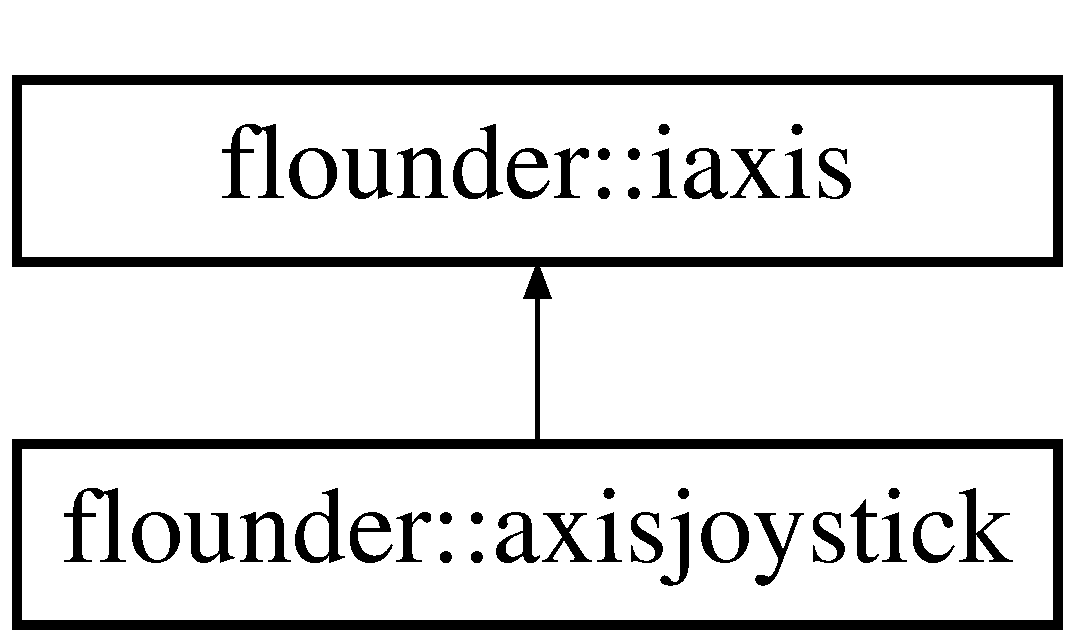
\includegraphics[height=2.000000cm]{classflounder_1_1iaxis}
\end{center}
\end{figure}
\subsection*{Public Member Functions}
\begin{DoxyCompactItemize}
\item 
virtual float \hyperlink{classflounder_1_1iaxis_a067a133edfde2ee8e2689df71328bf03}{get\+Amount} ()=0
\begin{DoxyCompactList}\small\item\em Gets the current value along the axis. -\/1 is smallest input, 1 is largest input. \end{DoxyCompactList}\end{DoxyCompactItemize}


\subsection{Detailed Description}
Interface for an axis based input device. 



\subsection{Member Function Documentation}
\mbox{\Hypertarget{classflounder_1_1iaxis_a067a133edfde2ee8e2689df71328bf03}\label{classflounder_1_1iaxis_a067a133edfde2ee8e2689df71328bf03}} 
\index{flounder\+::iaxis@{flounder\+::iaxis}!get\+Amount@{get\+Amount}}
\index{get\+Amount@{get\+Amount}!flounder\+::iaxis@{flounder\+::iaxis}}
\subsubsection{\texorpdfstring{get\+Amount()}{getAmount()}}
{\footnotesize\ttfamily virtual float flounder\+::iaxis\+::get\+Amount (\begin{DoxyParamCaption}{ }\end{DoxyParamCaption})\hspace{0.3cm}{\ttfamily [pure virtual]}}



Gets the current value along the axis. -\/1 is smallest input, 1 is largest input. 

\begin{DoxyReturn}{Returns}
The current value of the axis in the range (-\/1, 1). 
\end{DoxyReturn}


Implemented in \hyperlink{classflounder_1_1axisjoystick_ace3ec0cbb5c9958fe8e8fb6996fc81c3}{flounder\+::axisjoystick}.



The documentation for this class was generated from the following file\+:\begin{DoxyCompactItemize}
\item 
C\+:/\+Users/mattp/\+Documents/\+Flounder/\+Flounder\+Core/\+Sources/inputs/iaxis.\+h\end{DoxyCompactItemize}

\hypertarget{classflounder_1_1ibutton}{}\section{flounder\+:\+:ibutton Class Reference}
\label{classflounder_1_1ibutton}\index{flounder\+::ibutton@{flounder\+::ibutton}}


Interface for a binary input device.  




{\ttfamily \#include $<$ibutton.\+h$>$}

Inheritance diagram for flounder\+:\+:ibutton\+:\begin{figure}[H]
\begin{center}
\leavevmode
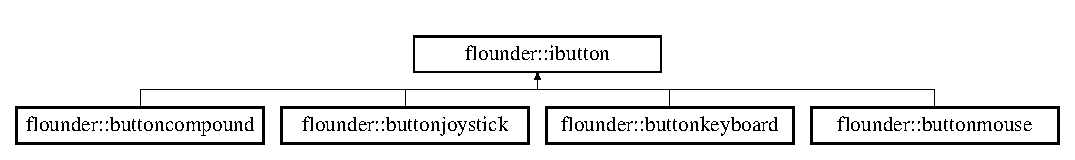
\includegraphics[height=2.000000cm]{classflounder_1_1ibutton}
\end{center}
\end{figure}
\subsection*{Public Member Functions}
\begin{DoxyCompactItemize}
\item 
virtual bool \hyperlink{classflounder_1_1ibutton_ab64fd22a75ea66ce67fd9b1ad34fd837}{is\+Down} ()=0
\begin{DoxyCompactList}\small\item\em Returns whether this button is currently pressed. \end{DoxyCompactList}\item 
virtual bool \hyperlink{classflounder_1_1ibutton_a5fb7b3493c0ea0e67bb9defc272da0d3}{was\+Down} ()=0
\begin{DoxyCompactList}\small\item\em Gets if the key is down and was not down before. Key press recognized as one click. \end{DoxyCompactList}\end{DoxyCompactItemize}


\subsection{Detailed Description}
Interface for a binary input device. 



\subsection{Member Function Documentation}
\mbox{\Hypertarget{classflounder_1_1ibutton_ab64fd22a75ea66ce67fd9b1ad34fd837}\label{classflounder_1_1ibutton_ab64fd22a75ea66ce67fd9b1ad34fd837}} 
\index{flounder\+::ibutton@{flounder\+::ibutton}!is\+Down@{is\+Down}}
\index{is\+Down@{is\+Down}!flounder\+::ibutton@{flounder\+::ibutton}}
\subsubsection{\texorpdfstring{is\+Down()}{isDown()}}
{\footnotesize\ttfamily virtual bool flounder\+::ibutton\+::is\+Down (\begin{DoxyParamCaption}{ }\end{DoxyParamCaption})\hspace{0.3cm}{\ttfamily [pure virtual]}}



Returns whether this button is currently pressed. 

\begin{DoxyReturn}{Returns}
True if the button is pressed, false otherwise. 
\end{DoxyReturn}


Implemented in \hyperlink{classflounder_1_1buttonjoystick_ab6682d3554e007ef473c4595339f86f1}{flounder\+::buttonjoystick}, \hyperlink{classflounder_1_1buttonkeyboard_a432555049251cec48431e4f14b6aa34b}{flounder\+::buttonkeyboard}, and \hyperlink{classflounder_1_1buttonmouse_ab4d7ecd54f144f03886b5ef467666be1}{flounder\+::buttonmouse}.

\mbox{\Hypertarget{classflounder_1_1ibutton_a5fb7b3493c0ea0e67bb9defc272da0d3}\label{classflounder_1_1ibutton_a5fb7b3493c0ea0e67bb9defc272da0d3}} 
\index{flounder\+::ibutton@{flounder\+::ibutton}!was\+Down@{was\+Down}}
\index{was\+Down@{was\+Down}!flounder\+::ibutton@{flounder\+::ibutton}}
\subsubsection{\texorpdfstring{was\+Down()}{wasDown()}}
{\footnotesize\ttfamily virtual bool flounder\+::ibutton\+::was\+Down (\begin{DoxyParamCaption}{ }\end{DoxyParamCaption})\hspace{0.3cm}{\ttfamily [pure virtual]}}



Gets if the key is down and was not down before. Key press recognized as one click. 

\begin{DoxyReturn}{Returns}
Is the key down and was not down before? 
\end{DoxyReturn}


Implemented in \hyperlink{classflounder_1_1buttonjoystick_a99302b1345fa773ec839290ae6c406e7}{flounder\+::buttonjoystick}, \hyperlink{classflounder_1_1buttonkeyboard_abc6b3c8cf9398f2a896408e390fd3a01}{flounder\+::buttonkeyboard}, and \hyperlink{classflounder_1_1buttonmouse_a7dad01481ebb01755db054a0acbc8159}{flounder\+::buttonmouse}.



The documentation for this class was generated from the following file\+:\begin{DoxyCompactItemize}
\item 
C\+:/\+Users/mattp/\+Documents/\+Flounder/\+Flounder\+Core/\+Sources/inputs/ibutton.\+h\end{DoxyCompactItemize}

\hypertarget{classflounder_1_1icamera}{}\section{flounder\+:\+:icamera Class Reference}
\label{classflounder_1_1icamera}\index{flounder\+::icamera@{flounder\+::icamera}}
\subsection*{Public Member Functions}
\begin{DoxyCompactItemize}
\item 
\mbox{\Hypertarget{classflounder_1_1icamera_a6595ce926a1d18c0df8c5a7b5665963d}\label{classflounder_1_1icamera_a6595ce926a1d18c0df8c5a7b5665963d}} 
virtual float \hyperlink{classflounder_1_1icamera_a6595ce926a1d18c0df8c5a7b5665963d}{get\+Near\+Plane} ()=0
\begin{DoxyCompactList}\small\item\em \begin{DoxyReturn}{Returns}
The distance of the near pane of the view frustum. 
\end{DoxyReturn}
\end{DoxyCompactList}\item 
\mbox{\Hypertarget{classflounder_1_1icamera_a682021a9ff1653ce4bf7288f94980633}\label{classflounder_1_1icamera_a682021a9ff1653ce4bf7288f94980633}} 
virtual float \hyperlink{classflounder_1_1icamera_a682021a9ff1653ce4bf7288f94980633}{get\+Far\+Plane} ()=0
\begin{DoxyCompactList}\small\item\em \begin{DoxyReturn}{Returns}
The distance of the view frustum\textquotesingle{}s far plane. 
\end{DoxyReturn}
\end{DoxyCompactList}\item 
\mbox{\Hypertarget{classflounder_1_1icamera_a60d622d1c9731da45bf49255dea95122}\label{classflounder_1_1icamera_a60d622d1c9731da45bf49255dea95122}} 
virtual float \hyperlink{classflounder_1_1icamera_a60d622d1c9731da45bf49255dea95122}{get\+F\+OV} ()=0
\begin{DoxyCompactList}\small\item\em \begin{DoxyReturn}{Returns}
The field of view angle for the view frustum. 
\end{DoxyReturn}
\end{DoxyCompactList}\item 
virtual void \hyperlink{classflounder_1_1icamera_ac7dc04e6fed5a9269c3d6ef11807fe99}{update} (\hyperlink{classflounder_1_1iplayer}{iplayer} $\ast$player)=0
\begin{DoxyCompactList}\small\item\em Checks inputs and carries out smooth camera movement. Should be called every frame. \end{DoxyCompactList}\item 
virtual \hyperlink{classflounder_1_1frustum}{frustum} $\ast$ \hyperlink{classflounder_1_1icamera_a6727d2cb720be2830e44ece8ad8e106b}{get\+View\+Frustum} ()=0
\begin{DoxyCompactList}\small\item\em Gets the view frustum created by the current camera position and rotation. \end{DoxyCompactList}\item 
virtual \hyperlink{classflounder_1_1ray}{ray} $\ast$ \hyperlink{classflounder_1_1icamera_a9b461abd1e1fd39127d3f2bc531aa847}{get\+View\+Ray} ()=0
\begin{DoxyCompactList}\small\item\em Gets the ray that extends from the cameras position though the screen. \end{DoxyCompactList}\item 
virtual \hyperlink{classflounder_1_1matrix4x4}{matrix4x4} $\ast$ \hyperlink{classflounder_1_1icamera_a64b4b040c903d37b3963aa2774c379db}{get\+View\+Matrix} ()=0
\begin{DoxyCompactList}\small\item\em Gets the view matrix created by the current camera position and rotation. \end{DoxyCompactList}\item 
virtual \hyperlink{classflounder_1_1matrix4x4}{matrix4x4} $\ast$ \hyperlink{classflounder_1_1icamera_a551908ec508ef29f1652c830cbe554f4}{get\+Projection\+Matrix} ()=0
\begin{DoxyCompactList}\small\item\em Gets the projection matrix used in the current scene render. \end{DoxyCompactList}\item 
virtual void \hyperlink{classflounder_1_1icamera_a20ee0d37d318012ac51e132ed02af6da}{reflect} (const float \&water\+Height)=0
\begin{DoxyCompactList}\small\item\em Prepares the camera for the reflection render pass. \end{DoxyCompactList}\item 
virtual \hyperlink{classflounder_1_1vector3}{vector3} $\ast$ \hyperlink{classflounder_1_1icamera_a1b3e1ee504b631da4baa1454304729e7}{get\+Position} ()=0
\begin{DoxyCompactList}\small\item\em Gets the cameras 3D position in the world. \end{DoxyCompactList}\item 
virtual \hyperlink{classflounder_1_1vector3}{vector3} $\ast$ \hyperlink{classflounder_1_1icamera_aa4d73bdf412e90c6d8747fc075568ff1}{get\+Rotation} ()=0
\begin{DoxyCompactList}\small\item\em Gets the cameras 3D rotation in the world, where x=pitch, y=yaw, z=roll. \end{DoxyCompactList}\item 
virtual void \hyperlink{classflounder_1_1icamera_abe51adbcadd5533bb1cd074d05179cd4}{set\+Rotation} (\hyperlink{classflounder_1_1vector3}{vector3} $\ast$rotation)=0
\begin{DoxyCompactList}\small\item\em Sets the rotation of the camera, where x=pitch, y=yaw, z=roll. \end{DoxyCompactList}\end{DoxyCompactItemize}


\subsection{Member Function Documentation}
\mbox{\Hypertarget{classflounder_1_1icamera_a1b3e1ee504b631da4baa1454304729e7}\label{classflounder_1_1icamera_a1b3e1ee504b631da4baa1454304729e7}} 
\index{flounder\+::icamera@{flounder\+::icamera}!get\+Position@{get\+Position}}
\index{get\+Position@{get\+Position}!flounder\+::icamera@{flounder\+::icamera}}
\subsubsection{\texorpdfstring{get\+Position()}{getPosition()}}
{\footnotesize\ttfamily virtual \hyperlink{classflounder_1_1vector3}{vector3}$\ast$ flounder\+::icamera\+::get\+Position (\begin{DoxyParamCaption}{ }\end{DoxyParamCaption})\hspace{0.3cm}{\ttfamily [pure virtual]}}



Gets the cameras 3D position in the world. 

\begin{DoxyReturn}{Returns}
The cameras 3D position in the world. 
\end{DoxyReturn}
\mbox{\Hypertarget{classflounder_1_1icamera_a551908ec508ef29f1652c830cbe554f4}\label{classflounder_1_1icamera_a551908ec508ef29f1652c830cbe554f4}} 
\index{flounder\+::icamera@{flounder\+::icamera}!get\+Projection\+Matrix@{get\+Projection\+Matrix}}
\index{get\+Projection\+Matrix@{get\+Projection\+Matrix}!flounder\+::icamera@{flounder\+::icamera}}
\subsubsection{\texorpdfstring{get\+Projection\+Matrix()}{getProjectionMatrix()}}
{\footnotesize\ttfamily virtual \hyperlink{classflounder_1_1matrix4x4}{matrix4x4}$\ast$ flounder\+::icamera\+::get\+Projection\+Matrix (\begin{DoxyParamCaption}{ }\end{DoxyParamCaption})\hspace{0.3cm}{\ttfamily [pure virtual]}}



Gets the projection matrix used in the current scene render. 

\begin{DoxyReturn}{Returns}
The projection matrix used in the current scene render. 
\end{DoxyReturn}
\mbox{\Hypertarget{classflounder_1_1icamera_aa4d73bdf412e90c6d8747fc075568ff1}\label{classflounder_1_1icamera_aa4d73bdf412e90c6d8747fc075568ff1}} 
\index{flounder\+::icamera@{flounder\+::icamera}!get\+Rotation@{get\+Rotation}}
\index{get\+Rotation@{get\+Rotation}!flounder\+::icamera@{flounder\+::icamera}}
\subsubsection{\texorpdfstring{get\+Rotation()}{getRotation()}}
{\footnotesize\ttfamily virtual \hyperlink{classflounder_1_1vector3}{vector3}$\ast$ flounder\+::icamera\+::get\+Rotation (\begin{DoxyParamCaption}{ }\end{DoxyParamCaption})\hspace{0.3cm}{\ttfamily [pure virtual]}}



Gets the cameras 3D rotation in the world, where x=pitch, y=yaw, z=roll. 

\begin{DoxyReturn}{Returns}
The cameras 3D rotation in the world, where x=pitch, y=yaw, z=roll. 
\end{DoxyReturn}
\mbox{\Hypertarget{classflounder_1_1icamera_a6727d2cb720be2830e44ece8ad8e106b}\label{classflounder_1_1icamera_a6727d2cb720be2830e44ece8ad8e106b}} 
\index{flounder\+::icamera@{flounder\+::icamera}!get\+View\+Frustum@{get\+View\+Frustum}}
\index{get\+View\+Frustum@{get\+View\+Frustum}!flounder\+::icamera@{flounder\+::icamera}}
\subsubsection{\texorpdfstring{get\+View\+Frustum()}{getViewFrustum()}}
{\footnotesize\ttfamily virtual \hyperlink{classflounder_1_1frustum}{frustum}$\ast$ flounder\+::icamera\+::get\+View\+Frustum (\begin{DoxyParamCaption}{ }\end{DoxyParamCaption})\hspace{0.3cm}{\ttfamily [pure virtual]}}



Gets the view frustum created by the current camera position and rotation. 

\begin{DoxyReturn}{Returns}
The view frustum created by the current camera position and rotation. 
\end{DoxyReturn}
\mbox{\Hypertarget{classflounder_1_1icamera_a64b4b040c903d37b3963aa2774c379db}\label{classflounder_1_1icamera_a64b4b040c903d37b3963aa2774c379db}} 
\index{flounder\+::icamera@{flounder\+::icamera}!get\+View\+Matrix@{get\+View\+Matrix}}
\index{get\+View\+Matrix@{get\+View\+Matrix}!flounder\+::icamera@{flounder\+::icamera}}
\subsubsection{\texorpdfstring{get\+View\+Matrix()}{getViewMatrix()}}
{\footnotesize\ttfamily virtual \hyperlink{classflounder_1_1matrix4x4}{matrix4x4}$\ast$ flounder\+::icamera\+::get\+View\+Matrix (\begin{DoxyParamCaption}{ }\end{DoxyParamCaption})\hspace{0.3cm}{\ttfamily [pure virtual]}}



Gets the view matrix created by the current camera position and rotation. 

\begin{DoxyReturn}{Returns}
The view matrix created by the current camera position and rotation. 
\end{DoxyReturn}
\mbox{\Hypertarget{classflounder_1_1icamera_a9b461abd1e1fd39127d3f2bc531aa847}\label{classflounder_1_1icamera_a9b461abd1e1fd39127d3f2bc531aa847}} 
\index{flounder\+::icamera@{flounder\+::icamera}!get\+View\+Ray@{get\+View\+Ray}}
\index{get\+View\+Ray@{get\+View\+Ray}!flounder\+::icamera@{flounder\+::icamera}}
\subsubsection{\texorpdfstring{get\+View\+Ray()}{getViewRay()}}
{\footnotesize\ttfamily virtual \hyperlink{classflounder_1_1ray}{ray}$\ast$ flounder\+::icamera\+::get\+View\+Ray (\begin{DoxyParamCaption}{ }\end{DoxyParamCaption})\hspace{0.3cm}{\ttfamily [pure virtual]}}



Gets the ray that extends from the cameras position though the screen. 

\begin{DoxyReturn}{Returns}
The cameras ray. 
\end{DoxyReturn}
\mbox{\Hypertarget{classflounder_1_1icamera_a20ee0d37d318012ac51e132ed02af6da}\label{classflounder_1_1icamera_a20ee0d37d318012ac51e132ed02af6da}} 
\index{flounder\+::icamera@{flounder\+::icamera}!reflect@{reflect}}
\index{reflect@{reflect}!flounder\+::icamera@{flounder\+::icamera}}
\subsubsection{\texorpdfstring{reflect()}{reflect()}}
{\footnotesize\ttfamily virtual void flounder\+::icamera\+::reflect (\begin{DoxyParamCaption}\item[{const float \&}]{water\+Height }\end{DoxyParamCaption})\hspace{0.3cm}{\ttfamily [pure virtual]}}



Prepares the camera for the reflection render pass. 


\begin{DoxyParams}{Parameters}
{\em water\+Height} & The height of the water to be reflected on. \\
\hline
\end{DoxyParams}
\mbox{\Hypertarget{classflounder_1_1icamera_abe51adbcadd5533bb1cd074d05179cd4}\label{classflounder_1_1icamera_abe51adbcadd5533bb1cd074d05179cd4}} 
\index{flounder\+::icamera@{flounder\+::icamera}!set\+Rotation@{set\+Rotation}}
\index{set\+Rotation@{set\+Rotation}!flounder\+::icamera@{flounder\+::icamera}}
\subsubsection{\texorpdfstring{set\+Rotation()}{setRotation()}}
{\footnotesize\ttfamily virtual void flounder\+::icamera\+::set\+Rotation (\begin{DoxyParamCaption}\item[{\hyperlink{classflounder_1_1vector3}{vector3} $\ast$}]{rotation }\end{DoxyParamCaption})\hspace{0.3cm}{\ttfamily [pure virtual]}}



Sets the rotation of the camera, where x=pitch, y=yaw, z=roll. 


\begin{DoxyParams}{Parameters}
{\em rotation} & The cameras new rotation. \\
\hline
\end{DoxyParams}
\mbox{\Hypertarget{classflounder_1_1icamera_ac7dc04e6fed5a9269c3d6ef11807fe99}\label{classflounder_1_1icamera_ac7dc04e6fed5a9269c3d6ef11807fe99}} 
\index{flounder\+::icamera@{flounder\+::icamera}!update@{update}}
\index{update@{update}!flounder\+::icamera@{flounder\+::icamera}}
\subsubsection{\texorpdfstring{update()}{update()}}
{\footnotesize\ttfamily virtual void flounder\+::icamera\+::update (\begin{DoxyParamCaption}\item[{\hyperlink{classflounder_1_1iplayer}{iplayer} $\ast$}]{player }\end{DoxyParamCaption})\hspace{0.3cm}{\ttfamily [pure virtual]}}



Checks inputs and carries out smooth camera movement. Should be called every frame. 


\begin{DoxyParams}{Parameters}
{\em player} & The movement and rotation controller to read from. \\
\hline
\end{DoxyParams}


The documentation for this class was generated from the following file\+:\begin{DoxyCompactItemize}
\item 
C\+:/\+Users/mattp/\+Documents/\+Flounder/\+Flounder\+Core/\+Sources/camera/icamera.\+h\end{DoxyCompactItemize}

\hypertarget{classflounder_1_1icollider}{}\section{flounder\+:\+:icollider Class Reference}
\label{classflounder_1_1icollider}\index{flounder\+::icollider@{flounder\+::icollider}}


A simple class that represents a physical shape.  




{\ttfamily \#include $<$icollider.\+h$>$}

Inheritance diagram for flounder\+:\+:icollider\+:\begin{figure}[H]
\begin{center}
\leavevmode
\includegraphics[height=2.000000cm]{classflounder_1_1icollider}
\end{center}
\end{figure}
\subsection*{Public Member Functions}
\begin{DoxyCompactItemize}
\item 
\hyperlink{classflounder_1_1icollider_a75adcd355b80f9def157cde97c89a1fe}{icollider} ()
\begin{DoxyCompactList}\small\item\em Creates a new collider. \end{DoxyCompactList}\item 
virtual \hyperlink{classflounder_1_1icollider_a8520c4acec0d91cd3d8bf1c381ad2da3}{$\sim$icollider} ()
\begin{DoxyCompactList}\small\item\em Deconstructor for the collider. \end{DoxyCompactList}\item 
virtual \hyperlink{classflounder_1_1icollider}{icollider} $\ast$ \hyperlink{classflounder_1_1icollider_a946ddd743680d0abc7b086d49f882e6f}{update} (const \hyperlink{classflounder_1_1vector3}{vector3} \&position, const \hyperlink{classflounder_1_1vector3}{vector3} \&rotation, const float \&scale, \hyperlink{classflounder_1_1icollider}{icollider} $\ast$destination)=0
\begin{DoxyCompactList}\small\item\em Clones this collder into the destination and updates it. \end{DoxyCompactList}\end{DoxyCompactItemize}


\subsection{Detailed Description}
A simple class that represents a physical shape. 



\subsection{Constructor \& Destructor Documentation}
\mbox{\Hypertarget{classflounder_1_1icollider_a75adcd355b80f9def157cde97c89a1fe}\label{classflounder_1_1icollider_a75adcd355b80f9def157cde97c89a1fe}} 
\index{flounder\+::icollider@{flounder\+::icollider}!icollider@{icollider}}
\index{icollider@{icollider}!flounder\+::icollider@{flounder\+::icollider}}
\subsubsection{\texorpdfstring{icollider()}{icollider()}}
{\footnotesize\ttfamily flounder\+::icollider\+::icollider (\begin{DoxyParamCaption}{ }\end{DoxyParamCaption})\hspace{0.3cm}{\ttfamily [inline]}}



Creates a new collider. 

\mbox{\Hypertarget{classflounder_1_1icollider_a8520c4acec0d91cd3d8bf1c381ad2da3}\label{classflounder_1_1icollider_a8520c4acec0d91cd3d8bf1c381ad2da3}} 
\index{flounder\+::icollider@{flounder\+::icollider}!````~icollider@{$\sim$icollider}}
\index{````~icollider@{$\sim$icollider}!flounder\+::icollider@{flounder\+::icollider}}
\subsubsection{\texorpdfstring{$\sim$icollider()}{~icollider()}}
{\footnotesize\ttfamily virtual flounder\+::icollider\+::$\sim$icollider (\begin{DoxyParamCaption}{ }\end{DoxyParamCaption})\hspace{0.3cm}{\ttfamily [inline]}, {\ttfamily [virtual]}}



Deconstructor for the collider. 



\subsection{Member Function Documentation}
\mbox{\Hypertarget{classflounder_1_1icollider_a946ddd743680d0abc7b086d49f882e6f}\label{classflounder_1_1icollider_a946ddd743680d0abc7b086d49f882e6f}} 
\index{flounder\+::icollider@{flounder\+::icollider}!update@{update}}
\index{update@{update}!flounder\+::icollider@{flounder\+::icollider}}
\subsubsection{\texorpdfstring{update()}{update()}}
{\footnotesize\ttfamily virtual \hyperlink{classflounder_1_1icollider}{icollider}$\ast$ flounder\+::icollider\+::update (\begin{DoxyParamCaption}\item[{const \hyperlink{classflounder_1_1vector3}{vector3} \&}]{position,  }\item[{const \hyperlink{classflounder_1_1vector3}{vector3} \&}]{rotation,  }\item[{const float \&}]{scale,  }\item[{\hyperlink{classflounder_1_1icollider}{icollider} $\ast$}]{destination }\end{DoxyParamCaption})\hspace{0.3cm}{\ttfamily [pure virtual]}}



Clones this collder into the destination and updates it. 


\begin{DoxyParams}{Parameters}
{\em position} & The amount to move. \\
\hline
{\em rotation} & The amount to rotate. \\
\hline
{\em scale} & The amount to scale the object. \\
\hline
{\em destination} & The collider to store the new data in. \\
\hline
\end{DoxyParams}
\begin{DoxyReturn}{Returns}
The destination. 
\end{DoxyReturn}


Implemented in \hyperlink{classflounder_1_1sphere_a9037b54ff10e6497a13f9836a77816fd}{flounder\+::sphere}.



The documentation for this class was generated from the following file\+:\begin{DoxyCompactItemize}
\item 
Flounder-\/\+Core/src/physics/icollider.\+h\end{DoxyCompactItemize}

\hypertarget{classflounder_1_1icomponent}{}\section{flounder\+:\+:icomponent Class Reference}
\label{classflounder_1_1icomponent}\index{flounder\+::icomponent@{flounder\+::icomponent}}
Inheritance diagram for flounder\+:\+:icomponent\+:\begin{figure}[H]
\begin{center}
\leavevmode
\includegraphics[height=2.000000cm]{classflounder_1_1icomponent}
\end{center}
\end{figure}
\subsection*{Public Member Functions}
\begin{DoxyCompactItemize}
\item 
\mbox{\Hypertarget{classflounder_1_1icomponent_af253f3dd7dea336348fe5b4f4da21d45}\label{classflounder_1_1icomponent_af253f3dd7dea336348fe5b4f4da21d45}} 
virtual void {\bfseries update} ()=0
\item 
\mbox{\Hypertarget{classflounder_1_1icomponent_a4edcb1b808fda7b1e85dd95eea3b656f}\label{classflounder_1_1icomponent_a4edcb1b808fda7b1e85dd95eea3b656f}} 
virtual void {\bfseries render} (\hyperlink{structflounder_1_1entityrender}{entityrender} $\ast$render)=0
\item 
\mbox{\Hypertarget{classflounder_1_1icomponent_aba3e4a5a9ffac336e13d0e3e0f89d6f7}\label{classflounder_1_1icomponent_aba3e4a5a9ffac336e13d0e3e0f89d6f7}} 
\hyperlink{classflounder_1_1entity}{entity} $\ast$ {\bfseries get\+Entity} () const
\item 
\mbox{\Hypertarget{classflounder_1_1icomponent_a3b589cf519260b286a5a6d5514a26795}\label{classflounder_1_1icomponent_a3b589cf519260b286a5a6d5514a26795}} 
void {\bfseries set\+Entity} (\hyperlink{classflounder_1_1entity}{entity} $\ast$\hyperlink{classflounder_1_1entity}{entity})
\end{DoxyCompactItemize}
\subsection*{Protected Attributes}
\begin{DoxyCompactItemize}
\item 
\mbox{\Hypertarget{classflounder_1_1icomponent_af5e25b049a691b4600e2058823a31c15}\label{classflounder_1_1icomponent_af5e25b049a691b4600e2058823a31c15}} 
\hyperlink{classflounder_1_1entity}{entity} $\ast$ {\bfseries m\+\_\+entity}
\end{DoxyCompactItemize}


The documentation for this class was generated from the following file\+:\begin{DoxyCompactItemize}
\item 
Flounder-\/\+Core/src/entities/icomponent.\+h\end{DoxyCompactItemize}

\hypertarget{classflounder_1_1idriver}{}\section{flounder\+:\+:idriver Class Reference}
\label{classflounder_1_1idriver}\index{flounder\+::idriver@{flounder\+::idriver}}


Represents a driver that changes over time.  




{\ttfamily \#include $<$idriver.\+h$>$}

Inheritance diagram for flounder\+:\+:idriver\+:\begin{figure}[H]
\begin{center}
\leavevmode
\includegraphics[height=1.212121cm]{classflounder_1_1idriver}
\end{center}
\end{figure}
\subsection*{Public Member Functions}
\begin{DoxyCompactItemize}
\item 
\hyperlink{classflounder_1_1idriver_a84bafd01e3984ededbb170a5efbad0f0}{idriver} (const float \&length)
\begin{DoxyCompactList}\small\item\em Creates a new driver with a length. \end{DoxyCompactList}\item 
virtual \hyperlink{classflounder_1_1idriver_a2a0111059b64474e6650b58d215defe0}{$\sim$idriver} ()
\begin{DoxyCompactList}\small\item\em Deconstructor for value driver. \end{DoxyCompactList}\item 
float \hyperlink{classflounder_1_1idriver_a1131c4e506fa5bfe3fae51b6636a09a9}{update} (const double \&\hyperlink{classflounder_1_1delta}{delta})
\begin{DoxyCompactList}\small\item\em Updates the driver with the passed time. \end{DoxyCompactList}\end{DoxyCompactItemize}
\subsection*{Protected Member Functions}
\begin{DoxyCompactItemize}
\item 
virtual float \hyperlink{classflounder_1_1idriver_a034c4159dc98c4c37ffdfaae64e4a16d}{calculate} (const float \&time)=0
\begin{DoxyCompactList}\small\item\em Calculates the new value. \end{DoxyCompactList}\item 
\mbox{\Hypertarget{classflounder_1_1idriver_a1b295944b61ae4ec6f312f842549294e}\label{classflounder_1_1idriver_a1b295944b61ae4ec6f312f842549294e}} 
float {\bfseries get\+Actual\+Time} ()
\end{DoxyCompactItemize}
\subsection*{Private Attributes}
\begin{DoxyCompactItemize}
\item 
\mbox{\Hypertarget{classflounder_1_1idriver_a24b0f7c3245fccec35c7bd8475501227}\label{classflounder_1_1idriver_a24b0f7c3245fccec35c7bd8475501227}} 
float {\bfseries m\+\_\+length}
\item 
\mbox{\Hypertarget{classflounder_1_1idriver_a323a95dedeb8e0a2c6e4a0e62268799f}\label{classflounder_1_1idriver_a323a95dedeb8e0a2c6e4a0e62268799f}} 
float {\bfseries m\+\_\+actual\+Time}
\item 
\mbox{\Hypertarget{classflounder_1_1idriver_a8b16f2ff43ceb60aeaf74dc0f137a829}\label{classflounder_1_1idriver_a8b16f2ff43ceb60aeaf74dc0f137a829}} 
float {\bfseries m\+\_\+current\+Time}
\end{DoxyCompactItemize}


\subsection{Detailed Description}
Represents a driver that changes over time. 



\subsection{Constructor \& Destructor Documentation}
\mbox{\Hypertarget{classflounder_1_1idriver_a84bafd01e3984ededbb170a5efbad0f0}\label{classflounder_1_1idriver_a84bafd01e3984ededbb170a5efbad0f0}} 
\index{flounder\+::idriver@{flounder\+::idriver}!idriver@{idriver}}
\index{idriver@{idriver}!flounder\+::idriver@{flounder\+::idriver}}
\subsubsection{\texorpdfstring{idriver()}{idriver()}}
{\footnotesize\ttfamily flounder\+::idriver\+::idriver (\begin{DoxyParamCaption}\item[{const float \&}]{length }\end{DoxyParamCaption})\hspace{0.3cm}{\ttfamily [inline]}}



Creates a new driver with a length. 


\begin{DoxyParams}{Parameters}
{\em length} & The drivers length. \\
\hline
\end{DoxyParams}
\mbox{\Hypertarget{classflounder_1_1idriver_a2a0111059b64474e6650b58d215defe0}\label{classflounder_1_1idriver_a2a0111059b64474e6650b58d215defe0}} 
\index{flounder\+::idriver@{flounder\+::idriver}!````~idriver@{$\sim$idriver}}
\index{````~idriver@{$\sim$idriver}!flounder\+::idriver@{flounder\+::idriver}}
\subsubsection{\texorpdfstring{$\sim$idriver()}{~idriver()}}
{\footnotesize\ttfamily virtual flounder\+::idriver\+::$\sim$idriver (\begin{DoxyParamCaption}{ }\end{DoxyParamCaption})\hspace{0.3cm}{\ttfamily [inline]}, {\ttfamily [virtual]}}



Deconstructor for value driver. 



\subsection{Member Function Documentation}
\mbox{\Hypertarget{classflounder_1_1idriver_a034c4159dc98c4c37ffdfaae64e4a16d}\label{classflounder_1_1idriver_a034c4159dc98c4c37ffdfaae64e4a16d}} 
\index{flounder\+::idriver@{flounder\+::idriver}!calculate@{calculate}}
\index{calculate@{calculate}!flounder\+::idriver@{flounder\+::idriver}}
\subsubsection{\texorpdfstring{calculate()}{calculate()}}
{\footnotesize\ttfamily virtual float flounder\+::idriver\+::calculate (\begin{DoxyParamCaption}\item[{const float \&}]{time }\end{DoxyParamCaption})\hspace{0.3cm}{\ttfamily [protected]}, {\ttfamily [pure virtual]}}



Calculates the new value. 


\begin{DoxyParams}{Parameters}
{\em time} & The time into the drivers life. \\
\hline
\end{DoxyParams}
\begin{DoxyReturn}{Returns}
The calculated value. 
\end{DoxyReturn}


Implemented in \hyperlink{classflounder_1_1driverfade_af0720c2a60e768dfa9702a43969bf65d}{flounder\+::driverfade}, \hyperlink{classflounder_1_1driverslide_aecbe9478f7ea9b1a781413f9284643c6}{flounder\+::driverslide}, \hyperlink{classflounder_1_1driverbounce_a2781832b47206849a0028ee75a4772e4}{flounder\+::driverbounce}, \hyperlink{classflounder_1_1driverlinear_a7f645c05d7a8bdb555bbf70aca7c630e}{flounder\+::driverlinear}, \hyperlink{classflounder_1_1driversinwave_ae5c3d8d4bd38082ad2b0396029d45e66}{flounder\+::driversinwave}, and \hyperlink{classflounder_1_1driverconstant_acf786b61ab46ea1ebf8d9a802c33c441}{flounder\+::driverconstant}.

\mbox{\Hypertarget{classflounder_1_1idriver_a1131c4e506fa5bfe3fae51b6636a09a9}\label{classflounder_1_1idriver_a1131c4e506fa5bfe3fae51b6636a09a9}} 
\index{flounder\+::idriver@{flounder\+::idriver}!update@{update}}
\index{update@{update}!flounder\+::idriver@{flounder\+::idriver}}
\subsubsection{\texorpdfstring{update()}{update()}}
{\footnotesize\ttfamily float flounder\+::idriver\+::update (\begin{DoxyParamCaption}\item[{const double \&}]{delta }\end{DoxyParamCaption})\hspace{0.3cm}{\ttfamily [inline]}}



Updates the driver with the passed time. 


\begin{DoxyParams}{Parameters}
{\em delta} & The time between the last update. \\
\hline
\end{DoxyParams}
\begin{DoxyReturn}{Returns}
The calculated value. 
\end{DoxyReturn}


The documentation for this class was generated from the following file\+:\begin{DoxyCompactItemize}
\item 
Flounder-\/\+Core/src/visual/idriver.\+h\end{DoxyCompactItemize}

\hypertarget{classflounder_1_1ievent}{}\section{flounder\+:\+:ievent Class Reference}
\label{classflounder_1_1ievent}\index{flounder\+::ievent@{flounder\+::ievent}}


A simple event listener and runner.  




{\ttfamily \#include $<$ievent.\+h$>$}

Inheritance diagram for flounder\+:\+:ievent\+:\begin{figure}[H]
\begin{center}
\leavevmode
\includegraphics[height=2.000000cm]{classflounder_1_1ievent}
\end{center}
\end{figure}
\subsection*{Public Member Functions}
\begin{DoxyCompactItemize}
\item 
\hyperlink{classflounder_1_1ievent_a87c44726337bd80b2b18a01ccdd562c6}{ievent} ()
\begin{DoxyCompactList}\small\item\em Creates a new event. \end{DoxyCompactList}\item 
virtual \hyperlink{classflounder_1_1ievent_af559376463c0e0643c67f8812169007c}{$\sim$ievent} ()
\begin{DoxyCompactList}\small\item\em Deconstructor for the event. \end{DoxyCompactList}\item 
virtual bool \hyperlink{classflounder_1_1ievent_a4462f66feef99ef4e3521c00f4edd0c9}{event\+Triggered} ()=0
\begin{DoxyCompactList}\small\item\em Gets if the event has occurred. \end{DoxyCompactList}\item 
virtual void \hyperlink{classflounder_1_1ievent_a6c6abe67435870b25eccd57a251a8992}{on\+Event} ()=0
\begin{DoxyCompactList}\small\item\em Run when a event has occurred. \end{DoxyCompactList}\item 
virtual bool \hyperlink{classflounder_1_1ievent_a7017c8803df2397758980cb61020e801}{remove\+After\+Event} ()=0
\begin{DoxyCompactList}\small\item\em Gets if the event is removed after it has run once. \end{DoxyCompactList}\end{DoxyCompactItemize}


\subsection{Detailed Description}
A simple event listener and runner. 



\subsection{Constructor \& Destructor Documentation}
\mbox{\Hypertarget{classflounder_1_1ievent_a87c44726337bd80b2b18a01ccdd562c6}\label{classflounder_1_1ievent_a87c44726337bd80b2b18a01ccdd562c6}} 
\index{flounder\+::ievent@{flounder\+::ievent}!ievent@{ievent}}
\index{ievent@{ievent}!flounder\+::ievent@{flounder\+::ievent}}
\subsubsection{\texorpdfstring{ievent()}{ievent()}}
{\footnotesize\ttfamily flounder\+::ievent\+::ievent (\begin{DoxyParamCaption}{ }\end{DoxyParamCaption})\hspace{0.3cm}{\ttfamily [inline]}}



Creates a new event. 

\mbox{\Hypertarget{classflounder_1_1ievent_af559376463c0e0643c67f8812169007c}\label{classflounder_1_1ievent_af559376463c0e0643c67f8812169007c}} 
\index{flounder\+::ievent@{flounder\+::ievent}!````~ievent@{$\sim$ievent}}
\index{````~ievent@{$\sim$ievent}!flounder\+::ievent@{flounder\+::ievent}}
\subsubsection{\texorpdfstring{$\sim$ievent()}{~ievent()}}
{\footnotesize\ttfamily virtual flounder\+::ievent\+::$\sim$ievent (\begin{DoxyParamCaption}{ }\end{DoxyParamCaption})\hspace{0.3cm}{\ttfamily [inline]}, {\ttfamily [virtual]}}



Deconstructor for the event. 



\subsection{Member Function Documentation}
\mbox{\Hypertarget{classflounder_1_1ievent_a4462f66feef99ef4e3521c00f4edd0c9}\label{classflounder_1_1ievent_a4462f66feef99ef4e3521c00f4edd0c9}} 
\index{flounder\+::ievent@{flounder\+::ievent}!event\+Triggered@{event\+Triggered}}
\index{event\+Triggered@{event\+Triggered}!flounder\+::ievent@{flounder\+::ievent}}
\subsubsection{\texorpdfstring{event\+Triggered()}{eventTriggered()}}
{\footnotesize\ttfamily virtual bool flounder\+::ievent\+::event\+Triggered (\begin{DoxyParamCaption}{ }\end{DoxyParamCaption})\hspace{0.3cm}{\ttfamily [pure virtual]}}



Gets if the event has occurred. 

\begin{DoxyReturn}{Returns}
The event has occurred. 
\end{DoxyReturn}


Implemented in \hyperlink{classflounder_1_1eventstandard_a88224b7246627df26a08ec9e286e7496}{flounder\+::eventstandard}, \hyperlink{classflounder_1_1eventtime_a67a616128c8e4701f7e229172c5e80a5}{flounder\+::eventtime}, and \hyperlink{classflounder_1_1eventchange_a2ae3c1f7ae4342dfff2aae6f11b0b413}{flounder\+::eventchange$<$ t $>$}.

\mbox{\Hypertarget{classflounder_1_1ievent_a6c6abe67435870b25eccd57a251a8992}\label{classflounder_1_1ievent_a6c6abe67435870b25eccd57a251a8992}} 
\index{flounder\+::ievent@{flounder\+::ievent}!on\+Event@{on\+Event}}
\index{on\+Event@{on\+Event}!flounder\+::ievent@{flounder\+::ievent}}
\subsubsection{\texorpdfstring{on\+Event()}{onEvent()}}
{\footnotesize\ttfamily virtual void flounder\+::ievent\+::on\+Event (\begin{DoxyParamCaption}{ }\end{DoxyParamCaption})\hspace{0.3cm}{\ttfamily [pure virtual]}}



Run when a event has occurred. 



Implemented in \hyperlink{classflounder_1_1eventstandard_af25e174b30e7d23698024b2c1ae9ac4c}{flounder\+::eventstandard}, \hyperlink{classflounder_1_1eventtime_a1b066c00fa959786bb1e9bbd1d212691}{flounder\+::eventtime}, and \hyperlink{classflounder_1_1eventchange_aa4fd4c3c28ac6927c3a810c8775f232d}{flounder\+::eventchange$<$ t $>$}.

\mbox{\Hypertarget{classflounder_1_1ievent_a7017c8803df2397758980cb61020e801}\label{classflounder_1_1ievent_a7017c8803df2397758980cb61020e801}} 
\index{flounder\+::ievent@{flounder\+::ievent}!remove\+After\+Event@{remove\+After\+Event}}
\index{remove\+After\+Event@{remove\+After\+Event}!flounder\+::ievent@{flounder\+::ievent}}
\subsubsection{\texorpdfstring{remove\+After\+Event()}{removeAfterEvent()}}
{\footnotesize\ttfamily virtual bool flounder\+::ievent\+::remove\+After\+Event (\begin{DoxyParamCaption}{ }\end{DoxyParamCaption})\hspace{0.3cm}{\ttfamily [pure virtual]}}



Gets if the event is removed after it has run once. 

\begin{DoxyReturn}{Returns}
If the even will run. 
\end{DoxyReturn}


Implemented in \hyperlink{classflounder_1_1eventstandard_ac4b9d57605f7f81c7c7e1cb981002f2f}{flounder\+::eventstandard}, \hyperlink{classflounder_1_1eventtime_ad765cd1e3b8fe2bf95f2290f5c625af1}{flounder\+::eventtime}, and \hyperlink{classflounder_1_1eventchange_ab3d476ecb51140e93886dc320ee44c33}{flounder\+::eventchange$<$ t $>$}.



The documentation for this class was generated from the following file\+:\begin{DoxyCompactItemize}
\item 
Flounder-\/\+Core/src/events/ievent.\+h\end{DoxyCompactItemize}

\hypertarget{classflounder_1_1igrabber}{}\section{flounder\+:\+:igrabber Class Reference}
\label{classflounder_1_1igrabber}\index{flounder\+::igrabber@{flounder\+::igrabber}}
Inheritance diagram for flounder\+:\+:igrabber\+:\begin{figure}[H]
\begin{center}
\leavevmode
\includegraphics[height=2.000000cm]{classflounder_1_1igrabber}
\end{center}
\end{figure}
\subsection*{Public Member Functions}
\begin{DoxyCompactItemize}
\item 
\mbox{\Hypertarget{classflounder_1_1igrabber_aeb322a326b59e5b04d02e51b450eb062}\label{classflounder_1_1igrabber_aeb322a326b59e5b04d02e51b450eb062}} 
virtual int {\bfseries get\+Current} (\hyperlink{classflounder_1_1text}{text} $\ast$object)=0
\item 
\mbox{\Hypertarget{classflounder_1_1igrabber_ac1940cd39641d67cba4417b81776bc26}\label{classflounder_1_1igrabber_ac1940cd39641d67cba4417b81776bc26}} 
virtual std\+::string {\bfseries get\+Value} (const int \&value)=0
\end{DoxyCompactItemize}


The documentation for this class was generated from the following file\+:\begin{DoxyCompactItemize}
\item 
Flounder-\/\+Core/src/uis/inputgrabber.\+h\end{DoxyCompactItemize}

\hypertarget{classflounder_1_1imanagerrender}{}\section{flounder\+:\+:imanagerrender Class Reference}
\label{classflounder_1_1imanagerrender}\index{flounder\+::imanagerrender@{flounder\+::imanagerrender}}


A extension used with irenderers to define a master renderer.  




{\ttfamily \#include $<$imanagerrender.\+h$>$}

\subsection*{Public Member Functions}
\begin{DoxyCompactItemize}
\item 
\hyperlink{classflounder_1_1imanagerrender_ada5d5c91beb519900e79957f631dc4e0}{imanagerrender} ()
\begin{DoxyCompactList}\small\item\em Creates a new master renderer. \end{DoxyCompactList}\item 
virtual \hyperlink{classflounder_1_1imanagerrender_abcc4d43e01ff6315c58a9df1b091aca0}{$\sim$imanagerrender} ()
\begin{DoxyCompactList}\small\item\em Deconstructor for the master renderer. \end{DoxyCompactList}\item 
virtual void \hyperlink{classflounder_1_1imanagerrender_a7cb8095219bd72cd974043adcbc908b4}{render} ()=0
\begin{DoxyCompactList}\small\item\em Run when rendering the master renderer. \end{DoxyCompactList}\end{DoxyCompactItemize}


\subsection{Detailed Description}
A extension used with irenderers to define a master renderer. 



\subsection{Constructor \& Destructor Documentation}
\mbox{\Hypertarget{classflounder_1_1imanagerrender_ada5d5c91beb519900e79957f631dc4e0}\label{classflounder_1_1imanagerrender_ada5d5c91beb519900e79957f631dc4e0}} 
\index{flounder\+::imanagerrender@{flounder\+::imanagerrender}!imanagerrender@{imanagerrender}}
\index{imanagerrender@{imanagerrender}!flounder\+::imanagerrender@{flounder\+::imanagerrender}}
\subsubsection{\texorpdfstring{imanagerrender()}{imanagerrender()}}
{\footnotesize\ttfamily flounder\+::imanagerrender\+::imanagerrender (\begin{DoxyParamCaption}{ }\end{DoxyParamCaption})\hspace{0.3cm}{\ttfamily [inline]}}



Creates a new master renderer. 

\mbox{\Hypertarget{classflounder_1_1imanagerrender_abcc4d43e01ff6315c58a9df1b091aca0}\label{classflounder_1_1imanagerrender_abcc4d43e01ff6315c58a9df1b091aca0}} 
\index{flounder\+::imanagerrender@{flounder\+::imanagerrender}!````~imanagerrender@{$\sim$imanagerrender}}
\index{````~imanagerrender@{$\sim$imanagerrender}!flounder\+::imanagerrender@{flounder\+::imanagerrender}}
\subsubsection{\texorpdfstring{$\sim$imanagerrender()}{~imanagerrender()}}
{\footnotesize\ttfamily virtual flounder\+::imanagerrender\+::$\sim$imanagerrender (\begin{DoxyParamCaption}{ }\end{DoxyParamCaption})\hspace{0.3cm}{\ttfamily [inline]}, {\ttfamily [virtual]}}



Deconstructor for the master renderer. 



\subsection{Member Function Documentation}
\mbox{\Hypertarget{classflounder_1_1imanagerrender_a7cb8095219bd72cd974043adcbc908b4}\label{classflounder_1_1imanagerrender_a7cb8095219bd72cd974043adcbc908b4}} 
\index{flounder\+::imanagerrender@{flounder\+::imanagerrender}!render@{render}}
\index{render@{render}!flounder\+::imanagerrender@{flounder\+::imanagerrender}}
\subsubsection{\texorpdfstring{render()}{render()}}
{\footnotesize\ttfamily virtual void flounder\+::imanagerrender\+::render (\begin{DoxyParamCaption}{ }\end{DoxyParamCaption})\hspace{0.3cm}{\ttfamily [pure virtual]}}



Run when rendering the master renderer. 



The documentation for this class was generated from the following file\+:\begin{DoxyCompactItemize}
\item 
Flounder-\/\+Core/src/renderer/imanagerrender.\+h\end{DoxyCompactItemize}

\hypertarget{classflounder_1_1imanageruis}{}\section{flounder\+:\+:imanageruis Class Reference}
\label{classflounder_1_1imanageruis}\index{flounder\+::imanageruis@{flounder\+::imanageruis}}


A interface used to manage a main UI system.  




{\ttfamily \#include $<$imanageruis.\+h$>$}

\subsection*{Public Member Functions}
\begin{DoxyCompactItemize}
\item 
\hyperlink{classflounder_1_1imanageruis_a11b6e709a8beb3a82f6febe132a7af1d}{imanageruis} ()
\begin{DoxyCompactList}\small\item\em Creates a new ui manager. \end{DoxyCompactList}\item 
virtual \hyperlink{classflounder_1_1imanageruis_adad4d9b86cea3db156f63e659faae623}{$\sim$imanageruis} ()
\begin{DoxyCompactList}\small\item\em Deconstructor for the ui manager. \end{DoxyCompactList}\item 
virtual void \hyperlink{classflounder_1_1imanageruis_a55a6b9eab0233c51c12b8819ba264b95}{update} ()=0
\begin{DoxyCompactList}\small\item\em Run when updating the ui manager. \end{DoxyCompactList}\item 
virtual bool \hyperlink{classflounder_1_1imanageruis_ad79a86978a96901e62ced2e0e0f09af3}{is\+Game\+Paused} ()=0
\begin{DoxyCompactList}\small\item\em Gets if the main menu is open. \end{DoxyCompactList}\item 
virtual float \hyperlink{classflounder_1_1imanageruis_a8acc9382f12a79893306145138034871}{get\+Blur\+Factor} ()=0
\begin{DoxyCompactList}\small\item\em Gets the main menu\textquotesingle{}s blur factor. \end{DoxyCompactList}\item 
virtual \hyperlink{classflounder_1_1colour}{colour} $\ast$ \hyperlink{classflounder_1_1imanageruis_add2f4d36a50adc177088f3a56c23a91a}{get\+Primary\+Colour} ()=0
\begin{DoxyCompactList}\small\item\em The primary colour to be used in UI elements. \end{DoxyCompactList}\end{DoxyCompactItemize}


\subsection{Detailed Description}
A interface used to manage a main UI system. 



\subsection{Constructor \& Destructor Documentation}
\mbox{\Hypertarget{classflounder_1_1imanageruis_a11b6e709a8beb3a82f6febe132a7af1d}\label{classflounder_1_1imanageruis_a11b6e709a8beb3a82f6febe132a7af1d}} 
\index{flounder\+::imanageruis@{flounder\+::imanageruis}!imanageruis@{imanageruis}}
\index{imanageruis@{imanageruis}!flounder\+::imanageruis@{flounder\+::imanageruis}}
\subsubsection{\texorpdfstring{imanageruis()}{imanageruis()}}
{\footnotesize\ttfamily flounder\+::imanageruis\+::imanageruis (\begin{DoxyParamCaption}{ }\end{DoxyParamCaption})\hspace{0.3cm}{\ttfamily [inline]}}



Creates a new ui manager. 

\mbox{\Hypertarget{classflounder_1_1imanageruis_adad4d9b86cea3db156f63e659faae623}\label{classflounder_1_1imanageruis_adad4d9b86cea3db156f63e659faae623}} 
\index{flounder\+::imanageruis@{flounder\+::imanageruis}!````~imanageruis@{$\sim$imanageruis}}
\index{````~imanageruis@{$\sim$imanageruis}!flounder\+::imanageruis@{flounder\+::imanageruis}}
\subsubsection{\texorpdfstring{$\sim$imanageruis()}{~imanageruis()}}
{\footnotesize\ttfamily virtual flounder\+::imanageruis\+::$\sim$imanageruis (\begin{DoxyParamCaption}{ }\end{DoxyParamCaption})\hspace{0.3cm}{\ttfamily [inline]}, {\ttfamily [virtual]}}



Deconstructor for the ui manager. 



\subsection{Member Function Documentation}
\mbox{\Hypertarget{classflounder_1_1imanageruis_a8acc9382f12a79893306145138034871}\label{classflounder_1_1imanageruis_a8acc9382f12a79893306145138034871}} 
\index{flounder\+::imanageruis@{flounder\+::imanageruis}!get\+Blur\+Factor@{get\+Blur\+Factor}}
\index{get\+Blur\+Factor@{get\+Blur\+Factor}!flounder\+::imanageruis@{flounder\+::imanageruis}}
\subsubsection{\texorpdfstring{get\+Blur\+Factor()}{getBlurFactor()}}
{\footnotesize\ttfamily virtual float flounder\+::imanageruis\+::get\+Blur\+Factor (\begin{DoxyParamCaption}{ }\end{DoxyParamCaption})\hspace{0.3cm}{\ttfamily [pure virtual]}}



Gets the main menu\textquotesingle{}s blur factor. 

\begin{DoxyReturn}{Returns}
The main menu\textquotesingle{}s blur factor. 
\end{DoxyReturn}
\mbox{\Hypertarget{classflounder_1_1imanageruis_add2f4d36a50adc177088f3a56c23a91a}\label{classflounder_1_1imanageruis_add2f4d36a50adc177088f3a56c23a91a}} 
\index{flounder\+::imanageruis@{flounder\+::imanageruis}!get\+Primary\+Colour@{get\+Primary\+Colour}}
\index{get\+Primary\+Colour@{get\+Primary\+Colour}!flounder\+::imanageruis@{flounder\+::imanageruis}}
\subsubsection{\texorpdfstring{get\+Primary\+Colour()}{getPrimaryColour()}}
{\footnotesize\ttfamily virtual \hyperlink{classflounder_1_1colour}{colour}$\ast$ flounder\+::imanageruis\+::get\+Primary\+Colour (\begin{DoxyParamCaption}{ }\end{DoxyParamCaption})\hspace{0.3cm}{\ttfamily [pure virtual]}}



The primary colour to be used in UI elements. 

\begin{DoxyReturn}{Returns}
The primary colour. 
\end{DoxyReturn}
\mbox{\Hypertarget{classflounder_1_1imanageruis_ad79a86978a96901e62ced2e0e0f09af3}\label{classflounder_1_1imanageruis_ad79a86978a96901e62ced2e0e0f09af3}} 
\index{flounder\+::imanageruis@{flounder\+::imanageruis}!is\+Game\+Paused@{is\+Game\+Paused}}
\index{is\+Game\+Paused@{is\+Game\+Paused}!flounder\+::imanageruis@{flounder\+::imanageruis}}
\subsubsection{\texorpdfstring{is\+Game\+Paused()}{isGamePaused()}}
{\footnotesize\ttfamily virtual bool flounder\+::imanageruis\+::is\+Game\+Paused (\begin{DoxyParamCaption}{ }\end{DoxyParamCaption})\hspace{0.3cm}{\ttfamily [pure virtual]}}



Gets if the main menu is open. 

\begin{DoxyReturn}{Returns}
If the main menu is open. 
\end{DoxyReturn}
\mbox{\Hypertarget{classflounder_1_1imanageruis_a55a6b9eab0233c51c12b8819ba264b95}\label{classflounder_1_1imanageruis_a55a6b9eab0233c51c12b8819ba264b95}} 
\index{flounder\+::imanageruis@{flounder\+::imanageruis}!update@{update}}
\index{update@{update}!flounder\+::imanageruis@{flounder\+::imanageruis}}
\subsubsection{\texorpdfstring{update()}{update()}}
{\footnotesize\ttfamily virtual void flounder\+::imanageruis\+::update (\begin{DoxyParamCaption}{ }\end{DoxyParamCaption})\hspace{0.3cm}{\ttfamily [pure virtual]}}



Run when updating the ui manager. 



The documentation for this class was generated from the following file\+:\begin{DoxyCompactItemize}
\item 
Flounder-\/\+Core/src/uis/imanageruis.\+h\end{DoxyCompactItemize}

\hypertarget{classflounder_1_1imodule}{}\section{flounder\+:\+:imodule Class Reference}
\label{classflounder_1_1imodule}\index{flounder\+::imodule@{flounder\+::imodule}}


A simple interface used for defining framework modules.  




{\ttfamily \#include $<$imodule.\+h$>$}

Inheritance diagram for flounder\+:\+:imodule\+:\begin{figure}[H]
\begin{center}
\leavevmode
\includegraphics[height=12.000000cm]{classflounder_1_1imodule}
\end{center}
\end{figure}
\subsection*{Public Member Functions}
\begin{DoxyCompactItemize}
\item 
\hyperlink{classflounder_1_1imodule_aa0b5648a6adbcf8c333820d967a37aeb}{imodule} ()
\begin{DoxyCompactList}\small\item\em Creates a new module. \end{DoxyCompactList}\item 
virtual \hyperlink{classflounder_1_1imodule_a519b8530d27d6c21d591e12e776ef834}{$\sim$imodule} ()
\begin{DoxyCompactList}\small\item\em Deconstructor for the module. \end{DoxyCompactList}\item 
virtual void \hyperlink{classflounder_1_1imodule_a9a53d48a46b5f6b16a92b2cd8503f74a}{update} ()=0
\begin{DoxyCompactList}\small\item\em The update function for the module. \end{DoxyCompactList}\end{DoxyCompactItemize}


\subsection{Detailed Description}
A simple interface used for defining framework modules. 



\subsection{Constructor \& Destructor Documentation}
\mbox{\Hypertarget{classflounder_1_1imodule_aa0b5648a6adbcf8c333820d967a37aeb}\label{classflounder_1_1imodule_aa0b5648a6adbcf8c333820d967a37aeb}} 
\index{flounder\+::imodule@{flounder\+::imodule}!imodule@{imodule}}
\index{imodule@{imodule}!flounder\+::imodule@{flounder\+::imodule}}
\subsubsection{\texorpdfstring{imodule()}{imodule()}}
{\footnotesize\ttfamily flounder\+::imodule\+::imodule (\begin{DoxyParamCaption}{ }\end{DoxyParamCaption})\hspace{0.3cm}{\ttfamily [inline]}}



Creates a new module. 

\mbox{\Hypertarget{classflounder_1_1imodule_a519b8530d27d6c21d591e12e776ef834}\label{classflounder_1_1imodule_a519b8530d27d6c21d591e12e776ef834}} 
\index{flounder\+::imodule@{flounder\+::imodule}!````~imodule@{$\sim$imodule}}
\index{````~imodule@{$\sim$imodule}!flounder\+::imodule@{flounder\+::imodule}}
\subsubsection{\texorpdfstring{$\sim$imodule()}{~imodule()}}
{\footnotesize\ttfamily virtual flounder\+::imodule\+::$\sim$imodule (\begin{DoxyParamCaption}{ }\end{DoxyParamCaption})\hspace{0.3cm}{\ttfamily [inline]}, {\ttfamily [virtual]}}



Deconstructor for the module. 



\subsection{Member Function Documentation}
\mbox{\Hypertarget{classflounder_1_1imodule_a9a53d48a46b5f6b16a92b2cd8503f74a}\label{classflounder_1_1imodule_a9a53d48a46b5f6b16a92b2cd8503f74a}} 
\index{flounder\+::imodule@{flounder\+::imodule}!update@{update}}
\index{update@{update}!flounder\+::imodule@{flounder\+::imodule}}
\subsubsection{\texorpdfstring{update()}{update()}}
{\footnotesize\ttfamily virtual void flounder\+::imodule\+::update (\begin{DoxyParamCaption}{ }\end{DoxyParamCaption})\hspace{0.3cm}{\ttfamily [pure virtual]}}



The update function for the module. 



Implemented in \hyperlink{classflounder_1_1display_a799c6a76fcac1a0ca56dfd6b8d7993fa}{flounder\+::display}, \hyperlink{classflounder_1_1audio_aabff6a1996b8571404023b6ac17009b6}{flounder\+::audio}, \hyperlink{classflounder_1_1renderer_aae85f1462ba4e9eb7899483536fdb0c5}{flounder\+::renderer}, \hyperlink{classflounder_1_1mouse_aa1b1d60e1d1cf4ec7d19eaef65e040bc}{flounder\+::mouse}, \hyperlink{classflounder_1_1shadows_ab8e8579cf14a761aad81566e98c51dec}{flounder\+::shadows}, \hyperlink{classflounder_1_1joysticks_a346fc03cae7164d6eb927333d1ae725f}{flounder\+::joysticks}, \hyperlink{classflounder_1_1uis_a234b52f70d1819932752a03168f21e10}{flounder\+::uis}, \hyperlink{classflounder_1_1particles_a12f1dd9883cc49987f6ff0ca3105bdb6}{flounder\+::particles}, \hyperlink{classflounder_1_1worlds_af1cdfac9ca2a2fc2768a9db4c1c22967}{flounder\+::worlds}, \hyperlink{classflounder_1_1waters_aaae93cea613594ea9d66819a63d4d85b}{flounder\+::waters}, \hyperlink{classflounder_1_1keyboard_a9fe79eabe905466fd90413d2c3b68841}{flounder\+::keyboard}, \hyperlink{classflounder_1_1processing_ac096299eb1b5b67739586900710d4206}{flounder\+::processing}, \hyperlink{classflounder_1_1camera_a6b2da3a1c348764d3cf954db5ac5b357}{flounder\+::camera}, \hyperlink{classflounder_1_1terrains_a4653233110b20bb5249a0913665928df}{flounder\+::terrains}, \hyperlink{classflounder_1_1events_a7fc08fdb5dc615a924dd0d55996747dc}{flounder\+::events}, \hyperlink{classflounder_1_1loaders_a9becf522a74f35f7e3dc7839577ba736}{flounder\+::loaders}, \hyperlink{classflounder_1_1standards_a681e682db67c10abb814cf0f8daf086a}{flounder\+::standards}, \hyperlink{classflounder_1_1skyboxes_ae94e675bcda78f2af0298a8551b82aa6}{flounder\+::skyboxes}, and \hyperlink{classflounder_1_1tasks_a32e51c65b63e8c98097d5d40c1912e5c}{flounder\+::tasks}.



The documentation for this class was generated from the following file\+:\begin{DoxyCompactItemize}
\item 
Flounder-\/\+Core/src/framework/imodule.\+h\end{DoxyCompactItemize}

\hypertarget{classflounder_1_1inputbutton}{}\section{flounder\+:\+:inputbutton Class Reference}
\label{classflounder_1_1inputbutton}\index{flounder\+::inputbutton@{flounder\+::inputbutton}}
Inheritance diagram for flounder\+:\+:inputbutton\+:\begin{figure}[H]
\begin{center}
\leavevmode
\includegraphics[height=2.000000cm]{classflounder_1_1inputbutton}
\end{center}
\end{figure}
\subsection*{Public Member Functions}
\begin{DoxyCompactItemize}
\item 
\mbox{\Hypertarget{classflounder_1_1inputbutton_a0f4deb8776c214858514e95578ca81c1}\label{classflounder_1_1inputbutton_a0f4deb8776c214858514e95578ca81c1}} 
{\bfseries inputbutton} (uiobject $\ast$parent, const \hyperlink{classflounder_1_1vector2}{vector2} \&position, const std\+::string \&string, const \hyperlink{namespaceflounder_a70f1871d5c05aa8e078dd37501ce10a9}{uialign} \&align)
\item 
\mbox{\Hypertarget{classflounder_1_1inputbutton_a8116aa642d04121dbebac91d0b074a96}\label{classflounder_1_1inputbutton_a8116aa642d04121dbebac91d0b074a96}} 
void {\bfseries update\+Object} () override
\item 
\mbox{\Hypertarget{classflounder_1_1inputbutton_a4ab362aa91ad5620d209174861c2306c}\label{classflounder_1_1inputbutton_a4ab362aa91ad5620d209174861c2306c}} 
std\+::string {\bfseries get\+Text} () const
\item 
\mbox{\Hypertarget{classflounder_1_1inputbutton_a1e7486b709c56a10c377576080b951c2}\label{classflounder_1_1inputbutton_a1e7486b709c56a10c377576080b951c2}} 
void {\bfseries set\+Text} (const std\+::string \&string) const
\item 
\mbox{\Hypertarget{classflounder_1_1inputbutton_a4cd73cfe3de3f2bc738659986cdf66d8}\label{classflounder_1_1inputbutton_a4cd73cfe3de3f2bc738659986cdf66d8}} 
void {\bfseries set\+Action\+Left} (std\+::function$<$ void()$>$ action)
\item 
\mbox{\Hypertarget{classflounder_1_1inputbutton_aa628f6d6413883b27dc8fd05275602c0}\label{classflounder_1_1inputbutton_aa628f6d6413883b27dc8fd05275602c0}} 
void {\bfseries set\+Action\+Right} (std\+::function$<$ void()$>$ action)
\end{DoxyCompactItemize}
\subsection*{Private Attributes}
\begin{DoxyCompactItemize}
\item 
\mbox{\Hypertarget{classflounder_1_1inputbutton_a926e89497fe3ccbda14181e7a4302e7c}\label{classflounder_1_1inputbutton_a926e89497fe3ccbda14181e7a4302e7c}} 
\hyperlink{classflounder_1_1text}{text} $\ast$ {\bfseries m\+\_\+text}
\item 
\mbox{\Hypertarget{classflounder_1_1inputbutton_aa643dc8120e533a926c8eaad49948153}\label{classflounder_1_1inputbutton_aa643dc8120e533a926c8eaad49948153}} 
\hyperlink{classflounder_1_1gui}{gui} $\ast$ {\bfseries m\+\_\+background}
\item 
\mbox{\Hypertarget{classflounder_1_1inputbutton_acaf1e6360396163866c798e555eb25c7}\label{classflounder_1_1inputbutton_acaf1e6360396163866c798e555eb25c7}} 
bool {\bfseries m\+\_\+mouse\+Over}
\item 
\mbox{\Hypertarget{classflounder_1_1inputbutton_a5ebc92aeb01736013eaa7fdd2833f525}\label{classflounder_1_1inputbutton_a5ebc92aeb01736013eaa7fdd2833f525}} 
std\+::function$<$ void()$>$ {\bfseries m\+\_\+action\+Left}
\item 
\mbox{\Hypertarget{classflounder_1_1inputbutton_aceff532fcea01bea6ee446d992e4d794}\label{classflounder_1_1inputbutton_aceff532fcea01bea6ee446d992e4d794}} 
std\+::function$<$ void()$>$ {\bfseries m\+\_\+action\+Right}
\end{DoxyCompactItemize}
\subsection*{Static Private Attributes}
\begin{DoxyCompactItemize}
\item 
\mbox{\Hypertarget{classflounder_1_1inputbutton_aa53987077c50fab936063854c997c121}\label{classflounder_1_1inputbutton_aa53987077c50fab936063854c997c121}} 
static const float {\bfseries C\+H\+A\+N\+G\+E\+\_\+\+T\+I\+ME} = 0.\+1f
\item 
\mbox{\Hypertarget{classflounder_1_1inputbutton_af37430ac9a5915cd2b1e6d41ddf30e5e}\label{classflounder_1_1inputbutton_af37430ac9a5915cd2b1e6d41ddf30e5e}} 
static const float {\bfseries S\+C\+A\+L\+E\+\_\+\+N\+O\+R\+M\+AL} = 1.\+6f
\item 
\mbox{\Hypertarget{classflounder_1_1inputbutton_a0c7575290d6017076f3049e8528fc94c}\label{classflounder_1_1inputbutton_a0c7575290d6017076f3049e8528fc94c}} 
static const float {\bfseries S\+C\+A\+L\+E\+\_\+\+S\+E\+L\+E\+C\+T\+ED} = 1.\+8f
\item 
\mbox{\Hypertarget{classflounder_1_1inputbutton_a02138feaaf1fcf1e71de1ffd1201c2ea}\label{classflounder_1_1inputbutton_a02138feaaf1fcf1e71de1ffd1201c2ea}} 
static \hyperlink{classflounder_1_1colour}{colour} $\ast$const {\bfseries C\+O\+L\+O\+U\+R\+\_\+\+N\+O\+R\+M\+AL} = new \hyperlink{classflounder_1_1colour}{colour}(0.\+0f, 0.\+0f, 0.\+0f)
\end{DoxyCompactItemize}


The documentation for this class was generated from the following files\+:\begin{DoxyCompactItemize}
\item 
Flounder-\/\+Core/src/uis/inputbutton.\+h\item 
Flounder-\/\+Core/src/uis/inputbutton.\+cpp\end{DoxyCompactItemize}

\hypertarget{classflounder_1_1inputdelay}{}\section{flounder\+:\+:inputdelay Class Reference}
\label{classflounder_1_1inputdelay}\index{flounder\+::inputdelay@{flounder\+::inputdelay}}
\subsection*{Public Member Functions}
\begin{DoxyCompactItemize}
\item 
\mbox{\Hypertarget{classflounder_1_1inputdelay_a28371a4f38cb5e70044aefccb3d7f651}\label{classflounder_1_1inputdelay_a28371a4f38cb5e70044aefccb3d7f651}} 
void {\bfseries update} (const bool \&key\+Is\+Down)
\item 
\mbox{\Hypertarget{classflounder_1_1inputdelay_a9ed02cf3bc03fe84401cad6396223664}\label{classflounder_1_1inputdelay_a9ed02cf3bc03fe84401cad6396223664}} 
bool {\bfseries can\+Input} ()
\end{DoxyCompactItemize}
\subsection*{Private Attributes}
\begin{DoxyCompactItemize}
\item 
\mbox{\Hypertarget{classflounder_1_1inputdelay_af06b9bb38cd1c07ca4ac225c5895a21e}\label{classflounder_1_1inputdelay_af06b9bb38cd1c07ca4ac225c5895a21e}} 
\hyperlink{classflounder_1_1timer}{timer} $\ast$ {\bfseries m\+\_\+timer\+Delay}
\item 
\mbox{\Hypertarget{classflounder_1_1inputdelay_a4c1e441caf57cf4cfd21488a9967c355}\label{classflounder_1_1inputdelay_a4c1e441caf57cf4cfd21488a9967c355}} 
\hyperlink{classflounder_1_1timer}{timer} $\ast$ {\bfseries m\+\_\+timer\+Repeat}
\item 
\mbox{\Hypertarget{classflounder_1_1inputdelay_ab37bc0a1daea38b2814cada46bb8417a}\label{classflounder_1_1inputdelay_ab37bc0a1daea38b2814cada46bb8417a}} 
bool {\bfseries m\+\_\+delay\+Over}
\end{DoxyCompactItemize}


The documentation for this class was generated from the following files\+:\begin{DoxyCompactItemize}
\item 
Flounder-\/\+Core/src/uis/inputdelay.\+h\item 
Flounder-\/\+Core/src/uis/inputdelay.\+cpp\end{DoxyCompactItemize}

\hypertarget{classflounder_1_1inputgrabber}{}\section{flounder\+:\+:inputgrabber Class Reference}
\label{classflounder_1_1inputgrabber}\index{flounder\+::inputgrabber@{flounder\+::inputgrabber}}
Inheritance diagram for flounder\+:\+:inputgrabber\+:\begin{figure}[H]
\begin{center}
\leavevmode
\includegraphics[height=2.000000cm]{classflounder_1_1inputgrabber}
\end{center}
\end{figure}
\subsection*{Public Member Functions}
\begin{DoxyCompactItemize}
\item 
\mbox{\Hypertarget{classflounder_1_1inputgrabber_a24c98328a702c7f1b08e5a4238bf582b}\label{classflounder_1_1inputgrabber_a24c98328a702c7f1b08e5a4238bf582b}} 
{\bfseries inputgrabber} (uiobject $\ast$parent, const \hyperlink{classflounder_1_1vector2}{vector2} \&position, const std\+::string \&prefix, const int \&value, \hyperlink{classflounder_1_1igrabber}{igrabber} $\ast$grabber, const \hyperlink{namespaceflounder_a70f1871d5c05aa8e078dd37501ce10a9}{uialign} \&align)
\item 
\mbox{\Hypertarget{classflounder_1_1inputgrabber_a407f628395380dbbed088a72070275be}\label{classflounder_1_1inputgrabber_a407f628395380dbbed088a72070275be}} 
void {\bfseries update\+Object} () override
\item 
\mbox{\Hypertarget{classflounder_1_1inputgrabber_af3aef3652b713be3e426d936cb760872}\label{classflounder_1_1inputgrabber_af3aef3652b713be3e426d936cb760872}} 
std\+::string {\bfseries get\+Prefix} () const
\item 
\mbox{\Hypertarget{classflounder_1_1inputgrabber_a57992f42cf715cf51ff7f8939460eea6}\label{classflounder_1_1inputgrabber_a57992f42cf715cf51ff7f8939460eea6}} 
void {\bfseries set\+Prefix} (const std\+::string \&prefix)
\item 
\mbox{\Hypertarget{classflounder_1_1inputgrabber_a5500491abfaf13a0f4b6f5423f814623}\label{classflounder_1_1inputgrabber_a5500491abfaf13a0f4b6f5423f814623}} 
int {\bfseries get\+Value} () const
\item 
\mbox{\Hypertarget{classflounder_1_1inputgrabber_af32f5813b6273019d2bf2515aaf88826}\label{classflounder_1_1inputgrabber_af32f5813b6273019d2bf2515aaf88826}} 
void {\bfseries set\+Value} (const int \&value)
\item 
\mbox{\Hypertarget{classflounder_1_1inputgrabber_a506c608651b423e3eba777f80e0295fb}\label{classflounder_1_1inputgrabber_a506c608651b423e3eba777f80e0295fb}} 
void {\bfseries set\+Action\+Change} (std\+::function$<$ void()$>$ action)
\end{DoxyCompactItemize}
\subsection*{Private Attributes}
\begin{DoxyCompactItemize}
\item 
\mbox{\Hypertarget{classflounder_1_1inputgrabber_a9a965db3d095f40a4d52a8713a376600}\label{classflounder_1_1inputgrabber_a9a965db3d095f40a4d52a8713a376600}} 
\hyperlink{classflounder_1_1text}{text} $\ast$ {\bfseries m\+\_\+text}
\item 
\mbox{\Hypertarget{classflounder_1_1inputgrabber_a8aac6d523097c2f1ff77b7fe35c9e368}\label{classflounder_1_1inputgrabber_a8aac6d523097c2f1ff77b7fe35c9e368}} 
\hyperlink{classflounder_1_1gui}{gui} $\ast$ {\bfseries m\+\_\+background}
\item 
\mbox{\Hypertarget{classflounder_1_1inputgrabber_ac93d7c723cfebae50f4724e7192cc132}\label{classflounder_1_1inputgrabber_ac93d7c723cfebae50f4724e7192cc132}} 
\hyperlink{classflounder_1_1igrabber}{igrabber} $\ast$ {\bfseries m\+\_\+grabber}
\item 
\mbox{\Hypertarget{classflounder_1_1inputgrabber_aadadca0cc347151888821224014c122b}\label{classflounder_1_1inputgrabber_aadadca0cc347151888821224014c122b}} 
std\+::string {\bfseries m\+\_\+prefix}
\item 
\mbox{\Hypertarget{classflounder_1_1inputgrabber_aed3312cd1f4fdd4f6ab305c112e3ad3a}\label{classflounder_1_1inputgrabber_aed3312cd1f4fdd4f6ab305c112e3ad3a}} 
int {\bfseries m\+\_\+value}
\item 
\mbox{\Hypertarget{classflounder_1_1inputgrabber_ab5a764ad815421a67a15e28d029d2566}\label{classflounder_1_1inputgrabber_ab5a764ad815421a67a15e28d029d2566}} 
\hyperlink{classflounder_1_1inputdelay}{inputdelay} $\ast$ {\bfseries m\+\_\+input\+Delay}
\item 
\mbox{\Hypertarget{classflounder_1_1inputgrabber_a2040838a8f4939a7e7adaed49c2f1729}\label{classflounder_1_1inputgrabber_a2040838a8f4939a7e7adaed49c2f1729}} 
int {\bfseries m\+\_\+last\+Key}
\item 
\mbox{\Hypertarget{classflounder_1_1inputgrabber_aa45f51dc3838d5941ec54d241ab84d66}\label{classflounder_1_1inputgrabber_aa45f51dc3838d5941ec54d241ab84d66}} 
bool {\bfseries m\+\_\+selected}
\item 
\mbox{\Hypertarget{classflounder_1_1inputgrabber_a4dc7ccf0eace872f0c0662301f6d6f54}\label{classflounder_1_1inputgrabber_a4dc7ccf0eace872f0c0662301f6d6f54}} 
bool {\bfseries m\+\_\+mouse\+Over}
\item 
\mbox{\Hypertarget{classflounder_1_1inputgrabber_a9b86cfa1cf976e763ea0a1a50f2a5b33}\label{classflounder_1_1inputgrabber_a9b86cfa1cf976e763ea0a1a50f2a5b33}} 
std\+::function$<$ void()$>$ {\bfseries m\+\_\+action\+Change}
\end{DoxyCompactItemize}
\subsection*{Static Private Attributes}
\begin{DoxyCompactItemize}
\item 
\mbox{\Hypertarget{classflounder_1_1inputgrabber_a3eb0f15e060b36939196d30aace889e2}\label{classflounder_1_1inputgrabber_a3eb0f15e060b36939196d30aace889e2}} 
static const float {\bfseries C\+H\+A\+N\+G\+E\+\_\+\+T\+I\+ME} = 0.\+1f
\item 
\mbox{\Hypertarget{classflounder_1_1inputgrabber_a1782b06602f89a1904eb45a6f19230f5}\label{classflounder_1_1inputgrabber_a1782b06602f89a1904eb45a6f19230f5}} 
static const float {\bfseries S\+C\+A\+L\+E\+\_\+\+N\+O\+R\+M\+AL} = 1.\+6f
\item 
\mbox{\Hypertarget{classflounder_1_1inputgrabber_ad97b9f57014d55128e0dbcef068c70ce}\label{classflounder_1_1inputgrabber_ad97b9f57014d55128e0dbcef068c70ce}} 
static const float {\bfseries S\+C\+A\+L\+E\+\_\+\+S\+E\+L\+E\+C\+T\+ED} = 1.\+8f
\item 
\mbox{\Hypertarget{classflounder_1_1inputgrabber_ac4fc1d45c2d9450f3b3d36c152a317c3}\label{classflounder_1_1inputgrabber_ac4fc1d45c2d9450f3b3d36c152a317c3}} 
static \hyperlink{classflounder_1_1colour}{colour} $\ast$const {\bfseries C\+O\+L\+O\+U\+R\+\_\+\+N\+O\+R\+M\+AL} = new \hyperlink{classflounder_1_1colour}{colour}(0.\+0f, 0.\+0f, 0.\+0f)
\end{DoxyCompactItemize}


The documentation for this class was generated from the following files\+:\begin{DoxyCompactItemize}
\item 
Flounder-\/\+Core/src/uis/inputgrabber.\+h\item 
Flounder-\/\+Core/src/uis/inputgrabber.\+cpp\end{DoxyCompactItemize}

\hypertarget{classflounder_1_1inputslider}{}\section{flounder\+:\+:inputslider Class Reference}
\label{classflounder_1_1inputslider}\index{flounder\+::inputslider@{flounder\+::inputslider}}
Inheritance diagram for flounder\+:\+:inputslider\+:\begin{figure}[H]
\begin{center}
\leavevmode
\includegraphics[height=2.000000cm]{classflounder_1_1inputslider}
\end{center}
\end{figure}
\subsection*{Public Member Functions}
\begin{DoxyCompactItemize}
\item 
\mbox{\Hypertarget{classflounder_1_1inputslider_acceb7f87ad9de910a40637462b717026}\label{classflounder_1_1inputslider_acceb7f87ad9de910a40637462b717026}} 
{\bfseries inputslider} (uiobject $\ast$parent, const \hyperlink{classflounder_1_1vector2}{vector2} \&position, const std\+::string \&string, const float \&progress\+Min, const float \&progress\+Max, const float \&value, const \hyperlink{namespaceflounder_a70f1871d5c05aa8e078dd37501ce10a9}{uialign} \&align)
\item 
\mbox{\Hypertarget{classflounder_1_1inputslider_aa4fab4980853dc11e84dc2fa30d32bd4}\label{classflounder_1_1inputslider_aa4fab4980853dc11e84dc2fa30d32bd4}} 
void {\bfseries update\+Object} () override
\item 
\mbox{\Hypertarget{classflounder_1_1inputslider_abb19ff9ca712ed80b5642294c0034f28}\label{classflounder_1_1inputslider_abb19ff9ca712ed80b5642294c0034f28}} 
std\+::string {\bfseries get\+Text} () const
\item 
\mbox{\Hypertarget{classflounder_1_1inputslider_a1f572b09075257e08b5e27fd8af4aeb3}\label{classflounder_1_1inputslider_a1f572b09075257e08b5e27fd8af4aeb3}} 
void {\bfseries set\+Text} (const std\+::string \&string) const
\item 
\mbox{\Hypertarget{classflounder_1_1inputslider_ad28da400c028c8ba35ead767ae192892}\label{classflounder_1_1inputslider_ad28da400c028c8ba35ead767ae192892}} 
float {\bfseries get\+Progress\+Min} () const
\item 
\mbox{\Hypertarget{classflounder_1_1inputslider_af7d08c95f39e9943e4e4eaa9d6be87b9}\label{classflounder_1_1inputslider_af7d08c95f39e9943e4e4eaa9d6be87b9}} 
void {\bfseries set\+Progress\+Min} (const float \&progress\+Min)
\item 
\mbox{\Hypertarget{classflounder_1_1inputslider_a48468b731d40bd79a9cf85aeb1e09be6}\label{classflounder_1_1inputslider_a48468b731d40bd79a9cf85aeb1e09be6}} 
float {\bfseries get\+Progress\+Max} () const
\item 
\mbox{\Hypertarget{classflounder_1_1inputslider_a8f146d939081c56aad47715f906e2d32}\label{classflounder_1_1inputslider_a8f146d939081c56aad47715f906e2d32}} 
void {\bfseries set\+Progress\+Max} (const float \&progress\+Max)
\item 
\mbox{\Hypertarget{classflounder_1_1inputslider_abfd79f6365d5498605040c4bf67939d6}\label{classflounder_1_1inputslider_abfd79f6365d5498605040c4bf67939d6}} 
float {\bfseries get\+Value} () const
\item 
\mbox{\Hypertarget{classflounder_1_1inputslider_a497557845fb46a5ff25fa6530a29eb8d}\label{classflounder_1_1inputslider_a497557845fb46a5ff25fa6530a29eb8d}} 
void {\bfseries set\+Value} (const float \&value)
\item 
\mbox{\Hypertarget{classflounder_1_1inputslider_a43b9cac2fa3624ed7d164910bf426be1}\label{classflounder_1_1inputslider_a43b9cac2fa3624ed7d164910bf426be1}} 
void {\bfseries set\+Action\+Change} (std\+::function$<$ void()$>$ action)
\end{DoxyCompactItemize}
\subsection*{Private Attributes}
\begin{DoxyCompactItemize}
\item 
\mbox{\Hypertarget{classflounder_1_1inputslider_a9e28205c0fab1bf8e494b963c340d83c}\label{classflounder_1_1inputslider_a9e28205c0fab1bf8e494b963c340d83c}} 
\hyperlink{classflounder_1_1text}{text} $\ast$ {\bfseries m\+\_\+text}
\item 
\mbox{\Hypertarget{classflounder_1_1inputslider_aee68e9a078ab5b62c2d6c5ad6e1c10f2}\label{classflounder_1_1inputslider_aee68e9a078ab5b62c2d6c5ad6e1c10f2}} 
\hyperlink{classflounder_1_1gui}{gui} $\ast$ {\bfseries m\+\_\+background}
\item 
\mbox{\Hypertarget{classflounder_1_1inputslider_a1384ef96c2b75a6b246f59c2aaadda87}\label{classflounder_1_1inputslider_a1384ef96c2b75a6b246f59c2aaadda87}} 
\hyperlink{classflounder_1_1gui}{gui} $\ast$ {\bfseries m\+\_\+slider}
\item 
\mbox{\Hypertarget{classflounder_1_1inputslider_a6c0742c879d8a2406942064cfa892e09}\label{classflounder_1_1inputslider_a6c0742c879d8a2406942064cfa892e09}} 
bool {\bfseries m\+\_\+updating}
\item 
\mbox{\Hypertarget{classflounder_1_1inputslider_a54f5c4f0f7cee761ee0b2bb28918a79e}\label{classflounder_1_1inputslider_a54f5c4f0f7cee761ee0b2bb28918a79e}} 
float {\bfseries m\+\_\+progress\+Min}
\item 
\mbox{\Hypertarget{classflounder_1_1inputslider_add88087e2175c685e1152bb2c10cd3c9}\label{classflounder_1_1inputslider_add88087e2175c685e1152bb2c10cd3c9}} 
float {\bfseries m\+\_\+progress\+Max}
\item 
\mbox{\Hypertarget{classflounder_1_1inputslider_abdd9aaa17fae957ba8ed7112aaef6458}\label{classflounder_1_1inputslider_abdd9aaa17fae957ba8ed7112aaef6458}} 
float {\bfseries m\+\_\+value}
\item 
\mbox{\Hypertarget{classflounder_1_1inputslider_ad23cd1bf4e920f052bf2bff00eb76847}\label{classflounder_1_1inputslider_ad23cd1bf4e920f052bf2bff00eb76847}} 
bool {\bfseries m\+\_\+mouse\+Over}
\item 
\mbox{\Hypertarget{classflounder_1_1inputslider_a7c6624912fd556cc78374b26c9990932}\label{classflounder_1_1inputslider_a7c6624912fd556cc78374b26c9990932}} 
bool {\bfseries m\+\_\+has\+Change}
\item 
\mbox{\Hypertarget{classflounder_1_1inputslider_ae9607a0738a6db00a2788d262691c4db}\label{classflounder_1_1inputslider_ae9607a0738a6db00a2788d262691c4db}} 
\hyperlink{classflounder_1_1timer}{timer} $\ast$ {\bfseries m\+\_\+timer\+Change}
\item 
\mbox{\Hypertarget{classflounder_1_1inputslider_a72579894648eb0081f92b8f5cfb8d4af}\label{classflounder_1_1inputslider_a72579894648eb0081f92b8f5cfb8d4af}} 
std\+::function$<$ void()$>$ {\bfseries m\+\_\+action\+Change}
\end{DoxyCompactItemize}
\subsection*{Static Private Attributes}
\begin{DoxyCompactItemize}
\item 
\mbox{\Hypertarget{classflounder_1_1inputslider_a95c103a84bc6ba6af9bd9fb5955b79f9}\label{classflounder_1_1inputslider_a95c103a84bc6ba6af9bd9fb5955b79f9}} 
static const float {\bfseries C\+H\+A\+N\+G\+E\+\_\+\+T\+I\+ME} = 0.\+1f
\item 
\mbox{\Hypertarget{classflounder_1_1inputslider_ae4521d9820984ce5e233b7fcdf398606}\label{classflounder_1_1inputslider_ae4521d9820984ce5e233b7fcdf398606}} 
static const float {\bfseries S\+C\+A\+L\+E\+\_\+\+N\+O\+R\+M\+AL} = 1.\+6f
\item 
\mbox{\Hypertarget{classflounder_1_1inputslider_aa37f8c17e01237ba7600489d23873105}\label{classflounder_1_1inputslider_aa37f8c17e01237ba7600489d23873105}} 
static const float {\bfseries S\+C\+A\+L\+E\+\_\+\+S\+E\+L\+E\+C\+T\+ED} = 1.\+8f
\item 
\mbox{\Hypertarget{classflounder_1_1inputslider_a507f8833ed23ebd4eeb83406f7023593}\label{classflounder_1_1inputslider_a507f8833ed23ebd4eeb83406f7023593}} 
static \hyperlink{classflounder_1_1colour}{colour} $\ast$const {\bfseries C\+O\+L\+O\+U\+R\+\_\+\+N\+O\+R\+M\+AL} = new \hyperlink{classflounder_1_1colour}{colour}(0.\+0f, 0.\+0f, 0.\+0f)
\end{DoxyCompactItemize}


The documentation for this class was generated from the following files\+:\begin{DoxyCompactItemize}
\item 
Flounder-\/\+Core/src/uis/inputslider.\+h\item 
Flounder-\/\+Core/src/uis/inputslider.\+cpp\end{DoxyCompactItemize}

\hypertarget{classflounder_1_1inputtext}{}\section{flounder\+:\+:inputtext Class Reference}
\label{classflounder_1_1inputtext}\index{flounder\+::inputtext@{flounder\+::inputtext}}
Inheritance diagram for flounder\+:\+:inputtext\+:\begin{figure}[H]
\begin{center}
\leavevmode
\includegraphics[height=2.000000cm]{classflounder_1_1inputtext}
\end{center}
\end{figure}
\subsection*{Public Member Functions}
\begin{DoxyCompactItemize}
\item 
\mbox{\Hypertarget{classflounder_1_1inputtext_aca56c185b95c971d82206985cd831bf6}\label{classflounder_1_1inputtext_aca56c185b95c971d82206985cd831bf6}} 
{\bfseries inputtext} (uiobject $\ast$parent, const \hyperlink{classflounder_1_1vector2}{vector2} \&position, const std\+::string \&prefix, const std\+::string \&value, const \hyperlink{namespaceflounder_a70f1871d5c05aa8e078dd37501ce10a9}{uialign} \&align)
\item 
\mbox{\Hypertarget{classflounder_1_1inputtext_a68496c28c8d375db5d9c2f1e7034c7e8}\label{classflounder_1_1inputtext_a68496c28c8d375db5d9c2f1e7034c7e8}} 
void {\bfseries update\+Object} () override
\item 
\mbox{\Hypertarget{classflounder_1_1inputtext_a96d00e15d518ff13c89b71b0a01caf4a}\label{classflounder_1_1inputtext_a96d00e15d518ff13c89b71b0a01caf4a}} 
std\+::string {\bfseries get\+Prefix} () const
\item 
\mbox{\Hypertarget{classflounder_1_1inputtext_a58321b833e8a09d930d3e254112e346a}\label{classflounder_1_1inputtext_a58321b833e8a09d930d3e254112e346a}} 
void {\bfseries set\+Prefix} (const std\+::string \&prefix)
\item 
\mbox{\Hypertarget{classflounder_1_1inputtext_a62ff597549d6a96e0d59cc6a6d2aa9d3}\label{classflounder_1_1inputtext_a62ff597549d6a96e0d59cc6a6d2aa9d3}} 
std\+::string {\bfseries get\+Value} () const
\item 
\mbox{\Hypertarget{classflounder_1_1inputtext_a4317b2a8a39dfd2e654b865191fc27cd}\label{classflounder_1_1inputtext_a4317b2a8a39dfd2e654b865191fc27cd}} 
void {\bfseries set\+Value} (const std\+::string \&value)
\item 
\mbox{\Hypertarget{classflounder_1_1inputtext_a9d643963d290e3c8e1de4d085a8de8e3}\label{classflounder_1_1inputtext_a9d643963d290e3c8e1de4d085a8de8e3}} 
void {\bfseries set\+Action\+Change} (std\+::function$<$ void()$>$ action)
\end{DoxyCompactItemize}
\subsection*{Private Attributes}
\begin{DoxyCompactItemize}
\item 
\mbox{\Hypertarget{classflounder_1_1inputtext_a4794f0a3d09dcc45a286f4eb3511ff3c}\label{classflounder_1_1inputtext_a4794f0a3d09dcc45a286f4eb3511ff3c}} 
\hyperlink{classflounder_1_1text}{text} $\ast$ {\bfseries m\+\_\+text}
\item 
\mbox{\Hypertarget{classflounder_1_1inputtext_aa0fdb585208f6385de300a3c11336d0b}\label{classflounder_1_1inputtext_aa0fdb585208f6385de300a3c11336d0b}} 
\hyperlink{classflounder_1_1gui}{gui} $\ast$ {\bfseries m\+\_\+background}
\item 
\mbox{\Hypertarget{classflounder_1_1inputtext_a4557935932e2527a470fafb6f8cdf178}\label{classflounder_1_1inputtext_a4557935932e2527a470fafb6f8cdf178}} 
std\+::string {\bfseries m\+\_\+prefix}
\item 
\mbox{\Hypertarget{classflounder_1_1inputtext_af88291b2fa2dfcb8f3dbace3f9dc4abd}\label{classflounder_1_1inputtext_af88291b2fa2dfcb8f3dbace3f9dc4abd}} 
std\+::string {\bfseries m\+\_\+value}
\item 
\mbox{\Hypertarget{classflounder_1_1inputtext_a1b03a7a75369059a684e0133adf8d7a0}\label{classflounder_1_1inputtext_a1b03a7a75369059a684e0133adf8d7a0}} 
\hyperlink{classflounder_1_1inputdelay}{inputdelay} $\ast$ {\bfseries m\+\_\+input\+Delay}
\item 
\mbox{\Hypertarget{classflounder_1_1inputtext_afd09ad8e2b567f08f86a18c3a8f3143e}\label{classflounder_1_1inputtext_afd09ad8e2b567f08f86a18c3a8f3143e}} 
int {\bfseries m\+\_\+last\+Key}
\item 
\mbox{\Hypertarget{classflounder_1_1inputtext_a6602ccd5d89133db62b79e113b83a44a}\label{classflounder_1_1inputtext_a6602ccd5d89133db62b79e113b83a44a}} 
bool {\bfseries m\+\_\+selected}
\item 
\mbox{\Hypertarget{classflounder_1_1inputtext_a58ff602dc0d034d89ff0b598b52c262d}\label{classflounder_1_1inputtext_a58ff602dc0d034d89ff0b598b52c262d}} 
bool {\bfseries m\+\_\+mouse\+Over}
\item 
\mbox{\Hypertarget{classflounder_1_1inputtext_af52da18a4fc81af17c310a1db85b8b38}\label{classflounder_1_1inputtext_af52da18a4fc81af17c310a1db85b8b38}} 
std\+::function$<$ void()$>$ {\bfseries m\+\_\+action\+Change}
\end{DoxyCompactItemize}
\subsection*{Static Private Attributes}
\begin{DoxyCompactItemize}
\item 
\mbox{\Hypertarget{classflounder_1_1inputtext_a82ca2663330304dbfe7eec79f7e0bdfa}\label{classflounder_1_1inputtext_a82ca2663330304dbfe7eec79f7e0bdfa}} 
static const float {\bfseries C\+H\+A\+N\+G\+E\+\_\+\+T\+I\+ME} = 0.\+1f
\item 
\mbox{\Hypertarget{classflounder_1_1inputtext_a052377a3ef7aab2b654dca4af3f6afc8}\label{classflounder_1_1inputtext_a052377a3ef7aab2b654dca4af3f6afc8}} 
static const float {\bfseries S\+C\+A\+L\+E\+\_\+\+N\+O\+R\+M\+AL} = 1.\+6f
\item 
\mbox{\Hypertarget{classflounder_1_1inputtext_a839f88d5217fe664f4d27e2c813a7b55}\label{classflounder_1_1inputtext_a839f88d5217fe664f4d27e2c813a7b55}} 
static const float {\bfseries S\+C\+A\+L\+E\+\_\+\+S\+E\+L\+E\+C\+T\+ED} = 1.\+8f
\item 
\mbox{\Hypertarget{classflounder_1_1inputtext_a52effd83ca83261bc2ebc8acd16279e7}\label{classflounder_1_1inputtext_a52effd83ca83261bc2ebc8acd16279e7}} 
static \hyperlink{classflounder_1_1colour}{colour} $\ast$const {\bfseries C\+O\+L\+O\+U\+R\+\_\+\+N\+O\+R\+M\+AL} = new \hyperlink{classflounder_1_1colour}{colour}(0.\+0f, 0.\+0f, 0.\+0f)
\end{DoxyCompactItemize}


The documentation for this class was generated from the following files\+:\begin{DoxyCompactItemize}
\item 
Flounder-\/\+Core/src/uis/inputtext.\+h\item 
Flounder-\/\+Core/src/uis/inputtext.\+cpp\end{DoxyCompactItemize}

\hypertarget{classflounder_1_1intersect}{}\section{flounder\+:\+:intersect Class Reference}
\label{classflounder_1_1intersect}\index{flounder\+::intersect@{flounder\+::intersect}}


A class that represents bounding intersect data.  




{\ttfamily \#include $<$intersect.\+h$>$}

\subsection*{Public Member Functions}
\begin{DoxyCompactItemize}
\item 
\hyperlink{classflounder_1_1intersect_a2c5914ddf56d123d8850fbfdba24d414}{intersect} (bool intersects, float distance)
\begin{DoxyCompactList}\small\item\em Creates a new bounding intersect data. \end{DoxyCompactList}\item 
\hyperlink{classflounder_1_1intersect_a9e7a429dfedbb9977ee512a3804eea94}{$\sim$intersect} ()
\begin{DoxyCompactList}\small\item\em Deconstructor for the intersect. \end{DoxyCompactList}\item 
bool \hyperlink{classflounder_1_1intersect_a680386b9684782d4b115ca380068ff3e}{is\+Intersection} ()
\begin{DoxyCompactList}\small\item\em Gets if there is a intersection. \end{DoxyCompactList}\item 
float \hyperlink{classflounder_1_1intersect_ab3f00d53d2614603bda044a43b27d679}{get\+Distance} ()
\begin{DoxyCompactList}\small\item\em Gets the distance that intersection is at. \end{DoxyCompactList}\end{DoxyCompactItemize}
\subsection*{Private Attributes}
\begin{DoxyCompactItemize}
\item 
\mbox{\Hypertarget{classflounder_1_1intersect_a897e4a28f81d86a82855f5a71de3dcbc}\label{classflounder_1_1intersect_a897e4a28f81d86a82855f5a71de3dcbc}} 
bool {\bfseries m\+\_\+intersects}
\item 
\mbox{\Hypertarget{classflounder_1_1intersect_abc36819adc7f0d5687b6b78995bb5e71}\label{classflounder_1_1intersect_abc36819adc7f0d5687b6b78995bb5e71}} 
float {\bfseries m\+\_\+distance}
\end{DoxyCompactItemize}


\subsection{Detailed Description}
A class that represents bounding intersect data. 



\subsection{Constructor \& Destructor Documentation}
\mbox{\Hypertarget{classflounder_1_1intersect_a2c5914ddf56d123d8850fbfdba24d414}\label{classflounder_1_1intersect_a2c5914ddf56d123d8850fbfdba24d414}} 
\index{flounder\+::intersect@{flounder\+::intersect}!intersect@{intersect}}
\index{intersect@{intersect}!flounder\+::intersect@{flounder\+::intersect}}
\subsubsection{\texorpdfstring{intersect()}{intersect()}}
{\footnotesize\ttfamily flounder\+::intersect\+::intersect (\begin{DoxyParamCaption}\item[{bool}]{intersects,  }\item[{float}]{distance }\end{DoxyParamCaption})\hspace{0.3cm}{\ttfamily [inline]}}



Creates a new bounding intersect data. 


\begin{DoxyParams}{Parameters}
{\em intersects} & If there is a collision. \\
\hline
{\em distance} & What distance that collision is at. \\
\hline
\end{DoxyParams}
\mbox{\Hypertarget{classflounder_1_1intersect_a9e7a429dfedbb9977ee512a3804eea94}\label{classflounder_1_1intersect_a9e7a429dfedbb9977ee512a3804eea94}} 
\index{flounder\+::intersect@{flounder\+::intersect}!````~intersect@{$\sim$intersect}}
\index{````~intersect@{$\sim$intersect}!flounder\+::intersect@{flounder\+::intersect}}
\subsubsection{\texorpdfstring{$\sim$intersect()}{~intersect()}}
{\footnotesize\ttfamily flounder\+::intersect\+::$\sim$intersect (\begin{DoxyParamCaption}{ }\end{DoxyParamCaption})\hspace{0.3cm}{\ttfamily [inline]}}



Deconstructor for the intersect. 



\subsection{Member Function Documentation}
\mbox{\Hypertarget{classflounder_1_1intersect_ab3f00d53d2614603bda044a43b27d679}\label{classflounder_1_1intersect_ab3f00d53d2614603bda044a43b27d679}} 
\index{flounder\+::intersect@{flounder\+::intersect}!get\+Distance@{get\+Distance}}
\index{get\+Distance@{get\+Distance}!flounder\+::intersect@{flounder\+::intersect}}
\subsubsection{\texorpdfstring{get\+Distance()}{getDistance()}}
{\footnotesize\ttfamily float flounder\+::intersect\+::get\+Distance (\begin{DoxyParamCaption}{ }\end{DoxyParamCaption})\hspace{0.3cm}{\ttfamily [inline]}}



Gets the distance that intersection is at. 

\begin{DoxyReturn}{Returns}
The distance that intersection is at. 
\end{DoxyReturn}
\mbox{\Hypertarget{classflounder_1_1intersect_a680386b9684782d4b115ca380068ff3e}\label{classflounder_1_1intersect_a680386b9684782d4b115ca380068ff3e}} 
\index{flounder\+::intersect@{flounder\+::intersect}!is\+Intersection@{is\+Intersection}}
\index{is\+Intersection@{is\+Intersection}!flounder\+::intersect@{flounder\+::intersect}}
\subsubsection{\texorpdfstring{is\+Intersection()}{isIntersection()}}
{\footnotesize\ttfamily bool flounder\+::intersect\+::is\+Intersection (\begin{DoxyParamCaption}{ }\end{DoxyParamCaption})\hspace{0.3cm}{\ttfamily [inline]}}



Gets if there is a intersection. 

\begin{DoxyReturn}{Returns}
If there is a intersection. 
\end{DoxyReturn}


The documentation for this class was generated from the following file\+:\begin{DoxyCompactItemize}
\item 
Flounder-\/\+Core/src/physics/intersect.\+h\end{DoxyCompactItemize}

\hypertarget{classflounder_1_1iplayer}{}\section{flounder\+:\+:iplayer Class Reference}
\label{classflounder_1_1iplayer}\index{flounder\+::iplayer@{flounder\+::iplayer}}


This interface is used to move and add extra rotation to a camera.  




{\ttfamily \#include $<$iplayer.\+h$>$}

\subsection*{Public Member Functions}
\begin{DoxyCompactItemize}
\item 
\hyperlink{classflounder_1_1iplayer_a5059d646c0397251c493c19c9a64f15a}{iplayer} ()
\begin{DoxyCompactList}\small\item\em Creates a new player. \end{DoxyCompactList}\item 
virtual \hyperlink{classflounder_1_1iplayer_af9dfb4e8585b475cc3178284e6815be1}{$\sim$iplayer} ()
\begin{DoxyCompactList}\small\item\em Deconstructor for the player. \end{DoxyCompactList}\item 
virtual void \hyperlink{classflounder_1_1iplayer_a763358c47f9d9433b0ce467418492038}{update} ()=0
\begin{DoxyCompactList}\small\item\em Checks inputs and carries out player movement. Should be called every frame. \end{DoxyCompactList}\item 
virtual \hyperlink{classflounder_1_1vector3}{vector3} $\ast$ \hyperlink{classflounder_1_1iplayer_a4e1ed034ef9590feccaaeec519cdf43b}{get\+Position} () const =0
\begin{DoxyCompactList}\small\item\em Gets the players 3D position in the world. \end{DoxyCompactList}\item 
virtual \hyperlink{classflounder_1_1vector3}{vector3} $\ast$ \hyperlink{classflounder_1_1iplayer_ae86318c75ebf593561cbbd82a94ef822}{get\+Rotation} () const =0
\begin{DoxyCompactList}\small\item\em Gets the players 3D rotation in the world, where x=pitch, y=yaw, z=roll. \end{DoxyCompactList}\end{DoxyCompactItemize}


\subsection{Detailed Description}
This interface is used to move and add extra rotation to a camera. 



\subsection{Constructor \& Destructor Documentation}
\mbox{\Hypertarget{classflounder_1_1iplayer_a5059d646c0397251c493c19c9a64f15a}\label{classflounder_1_1iplayer_a5059d646c0397251c493c19c9a64f15a}} 
\index{flounder\+::iplayer@{flounder\+::iplayer}!iplayer@{iplayer}}
\index{iplayer@{iplayer}!flounder\+::iplayer@{flounder\+::iplayer}}
\subsubsection{\texorpdfstring{iplayer()}{iplayer()}}
{\footnotesize\ttfamily flounder\+::iplayer\+::iplayer (\begin{DoxyParamCaption}{ }\end{DoxyParamCaption})\hspace{0.3cm}{\ttfamily [inline]}}



Creates a new player. 

\mbox{\Hypertarget{classflounder_1_1iplayer_af9dfb4e8585b475cc3178284e6815be1}\label{classflounder_1_1iplayer_af9dfb4e8585b475cc3178284e6815be1}} 
\index{flounder\+::iplayer@{flounder\+::iplayer}!````~iplayer@{$\sim$iplayer}}
\index{````~iplayer@{$\sim$iplayer}!flounder\+::iplayer@{flounder\+::iplayer}}
\subsubsection{\texorpdfstring{$\sim$iplayer()}{~iplayer()}}
{\footnotesize\ttfamily virtual flounder\+::iplayer\+::$\sim$iplayer (\begin{DoxyParamCaption}{ }\end{DoxyParamCaption})\hspace{0.3cm}{\ttfamily [inline]}, {\ttfamily [virtual]}}



Deconstructor for the player. 



\subsection{Member Function Documentation}
\mbox{\Hypertarget{classflounder_1_1iplayer_a4e1ed034ef9590feccaaeec519cdf43b}\label{classflounder_1_1iplayer_a4e1ed034ef9590feccaaeec519cdf43b}} 
\index{flounder\+::iplayer@{flounder\+::iplayer}!get\+Position@{get\+Position}}
\index{get\+Position@{get\+Position}!flounder\+::iplayer@{flounder\+::iplayer}}
\subsubsection{\texorpdfstring{get\+Position()}{getPosition()}}
{\footnotesize\ttfamily virtual \hyperlink{classflounder_1_1vector3}{vector3}$\ast$ flounder\+::iplayer\+::get\+Position (\begin{DoxyParamCaption}{ }\end{DoxyParamCaption}) const\hspace{0.3cm}{\ttfamily [pure virtual]}}



Gets the players 3D position in the world. 

\begin{DoxyReturn}{Returns}
The players 3D position in the world. 
\end{DoxyReturn}
\mbox{\Hypertarget{classflounder_1_1iplayer_ae86318c75ebf593561cbbd82a94ef822}\label{classflounder_1_1iplayer_ae86318c75ebf593561cbbd82a94ef822}} 
\index{flounder\+::iplayer@{flounder\+::iplayer}!get\+Rotation@{get\+Rotation}}
\index{get\+Rotation@{get\+Rotation}!flounder\+::iplayer@{flounder\+::iplayer}}
\subsubsection{\texorpdfstring{get\+Rotation()}{getRotation()}}
{\footnotesize\ttfamily virtual \hyperlink{classflounder_1_1vector3}{vector3}$\ast$ flounder\+::iplayer\+::get\+Rotation (\begin{DoxyParamCaption}{ }\end{DoxyParamCaption}) const\hspace{0.3cm}{\ttfamily [pure virtual]}}



Gets the players 3D rotation in the world, where x=pitch, y=yaw, z=roll. 

\begin{DoxyReturn}{Returns}
The players 3D rotation in the world, where x=pitch, y=yaw, z=roll. 
\end{DoxyReturn}
\mbox{\Hypertarget{classflounder_1_1iplayer_a763358c47f9d9433b0ce467418492038}\label{classflounder_1_1iplayer_a763358c47f9d9433b0ce467418492038}} 
\index{flounder\+::iplayer@{flounder\+::iplayer}!update@{update}}
\index{update@{update}!flounder\+::iplayer@{flounder\+::iplayer}}
\subsubsection{\texorpdfstring{update()}{update()}}
{\footnotesize\ttfamily virtual void flounder\+::iplayer\+::update (\begin{DoxyParamCaption}{ }\end{DoxyParamCaption})\hspace{0.3cm}{\ttfamily [pure virtual]}}



Checks inputs and carries out player movement. Should be called every frame. 



The documentation for this class was generated from the following file\+:\begin{DoxyCompactItemize}
\item 
Flounder-\/\+Core/src/camera/iplayer.\+h\end{DoxyCompactItemize}

\hypertarget{classflounder_1_1ipostfilter}{}\section{flounder\+:\+:ipostfilter Class Reference}
\label{classflounder_1_1ipostfilter}\index{flounder\+::ipostfilter@{flounder\+::ipostfilter}}


Represents a post effect shader and on application saves the result into a fbo.  




{\ttfamily \#include $<$ipostfilter.\+h$>$}

Inheritance diagram for flounder\+:\+:ipostfilter\+:\begin{figure}[H]
\begin{center}
\leavevmode
\includegraphics[height=12.000000cm]{classflounder_1_1ipostfilter}
\end{center}
\end{figure}
\subsection*{Public Member Functions}
\begin{DoxyCompactItemize}
\item 
\hyperlink{classflounder_1_1ipostfilter_a2c792b5d59c2b47b1f3b75a7a1404df0}{ipostfilter} (const std\+::string \&filter\+Name, const std\+::string \&fragment\+Shader, fbo $\ast$fbo)
\begin{DoxyCompactList}\small\item\em Creates a new post effect filter \end{DoxyCompactList}\item 
\hyperlink{classflounder_1_1ipostfilter_adb158fccda942f9d05ec2c21ea3f8654}{ipostfilter} (const std\+::string \&filter\+Name, const std\+::string \&fragment\+Shader)
\begin{DoxyCompactList}\small\item\em Creates a new post effect filter \end{DoxyCompactList}\item 
\hyperlink{classflounder_1_1ipostfilter_a45622b81739ebad815b69526a878b054}{ipostfilter} (\hyperlink{classflounder_1_1shader}{shader} $\ast$\hyperlink{classflounder_1_1shader}{shader}, fbo $\ast$fbo)
\begin{DoxyCompactList}\small\item\em Creates a new post effect filter \end{DoxyCompactList}\item 
\hyperlink{classflounder_1_1ipostfilter_a90d67fde6f8fe6ff4e3a7dba0fab418d}{ipostfilter} (\hyperlink{classflounder_1_1shader}{shader} $\ast$\hyperlink{classflounder_1_1shader}{shader})
\begin{DoxyCompactList}\small\item\em Creates a new post effect filter \end{DoxyCompactList}\item 
virtual \hyperlink{classflounder_1_1ipostfilter_aca15b2f21a5f07ddcff5dcad764e137c}{$\sim$ipostfilter} ()
\begin{DoxyCompactList}\small\item\em Deconstructor for the post filter. \end{DoxyCompactList}\item 
void \hyperlink{classflounder_1_1ipostfilter_a34cced83864d9d6b1c664a0337cd97b2}{apply\+Filter} (const int n\+\_\+args,...)
\begin{DoxyCompactList}\small\item\em Renders the filter to its fbo. \end{DoxyCompactList}\item 
void \hyperlink{classflounder_1_1ipostfilter_a59407e666a5f2ae9767b9fc0f0e25ced}{apply\+Filter} (const int n\+\_\+args, va\+\_\+list args)
\begin{DoxyCompactList}\small\item\em Renders the filter to its fbo. \end{DoxyCompactList}\item 
virtual void \hyperlink{classflounder_1_1ipostfilter_a9b658b4672718d5ac36539875bde722e}{store\+Values} ()=0
\begin{DoxyCompactList}\small\item\em Can be used to store values into the shader, this is called when the filter is applied and the shader has been already started. \end{DoxyCompactList}\item 
fbo $\ast$ \hyperlink{classflounder_1_1ipostfilter_ae074e279e1e3c6ddea5df8530802b08b}{get\+Fbo} () const
\begin{DoxyCompactList}\small\item\em Gets the fbo the filter rendered into. \end{DoxyCompactList}\end{DoxyCompactItemize}
\subsection*{Protected Attributes}
\begin{DoxyCompactItemize}
\item 
\mbox{\Hypertarget{classflounder_1_1ipostfilter_ab197a81f28df26a38b3302914d6f42fc}\label{classflounder_1_1ipostfilter_ab197a81f28df26a38b3302914d6f42fc}} 
\hyperlink{classflounder_1_1shader}{shader} $\ast$ {\bfseries m\+\_\+shader}
\item 
\mbox{\Hypertarget{classflounder_1_1ipostfilter_a654b609c29c61f0232126d47de77b00a}\label{classflounder_1_1ipostfilter_a654b609c29c61f0232126d47de77b00a}} 
fbo $\ast$ {\bfseries m\+\_\+fbo}
\item 
\mbox{\Hypertarget{classflounder_1_1ipostfilter_abf1adae588040bf18dd205f9296f92db}\label{classflounder_1_1ipostfilter_abf1adae588040bf18dd205f9296f92db}} 
\hyperlink{classflounder_1_1model}{model} $\ast$ {\bfseries m\+\_\+model}
\end{DoxyCompactItemize}


\subsection{Detailed Description}
Represents a post effect shader and on application saves the result into a fbo. 



\subsection{Constructor \& Destructor Documentation}
\mbox{\Hypertarget{classflounder_1_1ipostfilter_a2c792b5d59c2b47b1f3b75a7a1404df0}\label{classflounder_1_1ipostfilter_a2c792b5d59c2b47b1f3b75a7a1404df0}} 
\index{flounder\+::ipostfilter@{flounder\+::ipostfilter}!ipostfilter@{ipostfilter}}
\index{ipostfilter@{ipostfilter}!flounder\+::ipostfilter@{flounder\+::ipostfilter}}
\subsubsection{\texorpdfstring{ipostfilter()}{ipostfilter()}\hspace{0.1cm}{\footnotesize\ttfamily [1/4]}}
{\footnotesize\ttfamily flounder\+::ipostfilter\+::ipostfilter (\begin{DoxyParamCaption}\item[{const std\+::string \&}]{filter\+Name,  }\item[{const std\+::string \&}]{fragment\+Shader,  }\item[{fbo $\ast$}]{fbo }\end{DoxyParamCaption})}



Creates a new post effect filter 


\begin{DoxyParams}{Parameters}
{\em filter\+Name} & The name for the filter. \\
\hline
{\em fragment\+Shader} & The fragment shader file. \\
\hline
{\em fbo} & The fbo to render into. \\
\hline
\end{DoxyParams}
\mbox{\Hypertarget{classflounder_1_1ipostfilter_adb158fccda942f9d05ec2c21ea3f8654}\label{classflounder_1_1ipostfilter_adb158fccda942f9d05ec2c21ea3f8654}} 
\index{flounder\+::ipostfilter@{flounder\+::ipostfilter}!ipostfilter@{ipostfilter}}
\index{ipostfilter@{ipostfilter}!flounder\+::ipostfilter@{flounder\+::ipostfilter}}
\subsubsection{\texorpdfstring{ipostfilter()}{ipostfilter()}\hspace{0.1cm}{\footnotesize\ttfamily [2/4]}}
{\footnotesize\ttfamily flounder\+::ipostfilter\+::ipostfilter (\begin{DoxyParamCaption}\item[{const std\+::string \&}]{filter\+Name,  }\item[{const std\+::string \&}]{fragment\+Shader }\end{DoxyParamCaption})}



Creates a new post effect filter 


\begin{DoxyParams}{Parameters}
{\em filter\+Name} & The name for the filter. \\
\hline
{\em fragment\+Shader} & The fragment shader file. \\
\hline
\end{DoxyParams}
\mbox{\Hypertarget{classflounder_1_1ipostfilter_a45622b81739ebad815b69526a878b054}\label{classflounder_1_1ipostfilter_a45622b81739ebad815b69526a878b054}} 
\index{flounder\+::ipostfilter@{flounder\+::ipostfilter}!ipostfilter@{ipostfilter}}
\index{ipostfilter@{ipostfilter}!flounder\+::ipostfilter@{flounder\+::ipostfilter}}
\subsubsection{\texorpdfstring{ipostfilter()}{ipostfilter()}\hspace{0.1cm}{\footnotesize\ttfamily [3/4]}}
{\footnotesize\ttfamily flounder\+::ipostfilter\+::ipostfilter (\begin{DoxyParamCaption}\item[{\hyperlink{classflounder_1_1shader}{shader} $\ast$}]{shader,  }\item[{fbo $\ast$}]{fbo }\end{DoxyParamCaption})}



Creates a new post effect filter 


\begin{DoxyParams}{Parameters}
{\em shader} & The shader for the filter. \\
\hline
{\em fbo} & The fbo to render into. \\
\hline
\end{DoxyParams}
\mbox{\Hypertarget{classflounder_1_1ipostfilter_a90d67fde6f8fe6ff4e3a7dba0fab418d}\label{classflounder_1_1ipostfilter_a90d67fde6f8fe6ff4e3a7dba0fab418d}} 
\index{flounder\+::ipostfilter@{flounder\+::ipostfilter}!ipostfilter@{ipostfilter}}
\index{ipostfilter@{ipostfilter}!flounder\+::ipostfilter@{flounder\+::ipostfilter}}
\subsubsection{\texorpdfstring{ipostfilter()}{ipostfilter()}\hspace{0.1cm}{\footnotesize\ttfamily [4/4]}}
{\footnotesize\ttfamily flounder\+::ipostfilter\+::ipostfilter (\begin{DoxyParamCaption}\item[{\hyperlink{classflounder_1_1shader}{shader} $\ast$}]{shader }\end{DoxyParamCaption})}



Creates a new post effect filter 


\begin{DoxyParams}{Parameters}
{\em shader} & The shader for the filter. \\
\hline
\end{DoxyParams}
\mbox{\Hypertarget{classflounder_1_1ipostfilter_aca15b2f21a5f07ddcff5dcad764e137c}\label{classflounder_1_1ipostfilter_aca15b2f21a5f07ddcff5dcad764e137c}} 
\index{flounder\+::ipostfilter@{flounder\+::ipostfilter}!````~ipostfilter@{$\sim$ipostfilter}}
\index{````~ipostfilter@{$\sim$ipostfilter}!flounder\+::ipostfilter@{flounder\+::ipostfilter}}
\subsubsection{\texorpdfstring{$\sim$ipostfilter()}{~ipostfilter()}}
{\footnotesize\ttfamily flounder\+::ipostfilter\+::$\sim$ipostfilter (\begin{DoxyParamCaption}{ }\end{DoxyParamCaption})\hspace{0.3cm}{\ttfamily [virtual]}}



Deconstructor for the post filter. 



\subsection{Member Function Documentation}
\mbox{\Hypertarget{classflounder_1_1ipostfilter_a34cced83864d9d6b1c664a0337cd97b2}\label{classflounder_1_1ipostfilter_a34cced83864d9d6b1c664a0337cd97b2}} 
\index{flounder\+::ipostfilter@{flounder\+::ipostfilter}!apply\+Filter@{apply\+Filter}}
\index{apply\+Filter@{apply\+Filter}!flounder\+::ipostfilter@{flounder\+::ipostfilter}}
\subsubsection{\texorpdfstring{apply\+Filter()}{applyFilter()}\hspace{0.1cm}{\footnotesize\ttfamily [1/2]}}
{\footnotesize\ttfamily void flounder\+::ipostfilter\+::apply\+Filter (\begin{DoxyParamCaption}\item[{const int}]{n\+\_\+args,  }\item[{}]{... }\end{DoxyParamCaption})}



Renders the filter to its fbo. 


\begin{DoxyParams}{Parameters}
{\em n\+\_\+args} & The number textures being bound to the shader. \\
\hline
{\em ...} & The textures being bound to the shader. \\
\hline
\end{DoxyParams}
\mbox{\Hypertarget{classflounder_1_1ipostfilter_a59407e666a5f2ae9767b9fc0f0e25ced}\label{classflounder_1_1ipostfilter_a59407e666a5f2ae9767b9fc0f0e25ced}} 
\index{flounder\+::ipostfilter@{flounder\+::ipostfilter}!apply\+Filter@{apply\+Filter}}
\index{apply\+Filter@{apply\+Filter}!flounder\+::ipostfilter@{flounder\+::ipostfilter}}
\subsubsection{\texorpdfstring{apply\+Filter()}{applyFilter()}\hspace{0.1cm}{\footnotesize\ttfamily [2/2]}}
{\footnotesize\ttfamily void flounder\+::ipostfilter\+::apply\+Filter (\begin{DoxyParamCaption}\item[{const int}]{n\+\_\+args,  }\item[{va\+\_\+list}]{args }\end{DoxyParamCaption})}



Renders the filter to its fbo. 


\begin{DoxyParams}{Parameters}
{\em n\+\_\+args} & The number textures being bound to the shader. \\
\hline
{\em ...} & The textures being bound to the shader. \\
\hline
\end{DoxyParams}
\mbox{\Hypertarget{classflounder_1_1ipostfilter_ae074e279e1e3c6ddea5df8530802b08b}\label{classflounder_1_1ipostfilter_ae074e279e1e3c6ddea5df8530802b08b}} 
\index{flounder\+::ipostfilter@{flounder\+::ipostfilter}!get\+Fbo@{get\+Fbo}}
\index{get\+Fbo@{get\+Fbo}!flounder\+::ipostfilter@{flounder\+::ipostfilter}}
\subsubsection{\texorpdfstring{get\+Fbo()}{getFbo()}}
{\footnotesize\ttfamily fbo$\ast$ flounder\+::ipostfilter\+::get\+Fbo (\begin{DoxyParamCaption}{ }\end{DoxyParamCaption}) const\hspace{0.3cm}{\ttfamily [inline]}}



Gets the fbo the filter rendered into. 

\begin{DoxyReturn}{Returns}
The fbo. 
\end{DoxyReturn}
\mbox{\Hypertarget{classflounder_1_1ipostfilter_a9b658b4672718d5ac36539875bde722e}\label{classflounder_1_1ipostfilter_a9b658b4672718d5ac36539875bde722e}} 
\index{flounder\+::ipostfilter@{flounder\+::ipostfilter}!store\+Values@{store\+Values}}
\index{store\+Values@{store\+Values}!flounder\+::ipostfilter@{flounder\+::ipostfilter}}
\subsubsection{\texorpdfstring{store\+Values()}{storeValues()}}
{\footnotesize\ttfamily virtual void flounder\+::ipostfilter\+::store\+Values (\begin{DoxyParamCaption}{ }\end{DoxyParamCaption})\hspace{0.3cm}{\ttfamily [pure virtual]}}



Can be used to store values into the shader, this is called when the filter is applied and the shader has been already started. 



Implemented in \hyperlink{classflounder_1_1filterblurhorizontal_ad147fceebdebffd0731fc346370021f7}{flounder\+::filterblurhorizontal}, \hyperlink{classflounder_1_1filterblurvertical_acdc191b6c9b067c9619055c1672dd2e5}{flounder\+::filterblurvertical}, \hyperlink{classflounder_1_1filtertiltshift_a8e04e52da882a2d78d7a0e1f70717114}{flounder\+::filtertiltshift}, \hyperlink{classflounder_1_1filtercrt_a6b3d151d6e338a7c859aeea1016724dc}{flounder\+::filtercrt}, \hyperlink{classflounder_1_1filterwobble_aa89ed7a9f3ad52790223b558aaff0cc4}{flounder\+::filterwobble}, \hyperlink{classflounder_1_1filterlensflare_a2ab19cc2427e840c9ae11fc004e963be}{flounder\+::filterlensflare}, \hyperlink{classflounder_1_1filterdarken_a5cee7990cb4de781465cf43f4695e823}{flounder\+::filterdarken}, \hyperlink{classflounder_1_1filtermotion_a6e8b5a9ce3660ab57fbb487fe6752acb}{flounder\+::filtermotion}, \hyperlink{classflounder_1_1filterpixel_abc7ae2b0a9bffd4986a664b690aab416}{flounder\+::filterpixel}, \hyperlink{classflounder_1_1filtercombine_a0ec0634422d3ed539045d9fcfa3d119e}{flounder\+::filtercombine}, \hyperlink{classflounder_1_1filterfxaa_abee255cfd538d96881386157e6e8eea0}{flounder\+::filterfxaa}, \hyperlink{classflounder_1_1filtergrain_a0f65f9e8b994f18a4777e4451bdf8b4e}{flounder\+::filtergrain}, \hyperlink{classflounder_1_1filterdefault_a9e858528a7d3356b94e16f10928a1d72}{flounder\+::filterdefault}, \hyperlink{classflounder_1_1filterbloom1_adfa3f732b13f449745418bf9bd539f79}{flounder\+::filterbloom1}, \hyperlink{classflounder_1_1filterbloom2_a6439fc5d762213a5f780033d6b88428e}{flounder\+::filterbloom2}, \hyperlink{classflounder_1_1filteremboss_aa0c7d249c2c830036904bede59dababf}{flounder\+::filteremboss}, \hyperlink{classflounder_1_1filtergrey_a927f448820b39299eb04c947ffdce671}{flounder\+::filtergrey}, \hyperlink{classflounder_1_1filternegative_abc832140c4d75f4684d3470e070bcf7a}{flounder\+::filternegative}, \hyperlink{classflounder_1_1filtersepia_a92d9cee7e92200212f40ff39f5cbc67f}{flounder\+::filtersepia}, and \hyperlink{classflounder_1_1filtertone_ad2b3b402d4f9fd38f918b410652ee96b}{flounder\+::filtertone}.



The documentation for this class was generated from the following files\+:\begin{DoxyCompactItemize}
\item 
Flounder-\/\+Core/src/post/ipostfilter.\+h\item 
Flounder-\/\+Core/src/post/ipostfilter.\+cpp\end{DoxyCompactItemize}

\hypertarget{classflounder_1_1ipostpipeline}{}\section{flounder\+:\+:ipostpipeline Class Reference}
\label{classflounder_1_1ipostpipeline}\index{flounder\+::ipostpipeline@{flounder\+::ipostpipeline}}


Represents a system of post effects.  




{\ttfamily \#include $<$ipostpipeline.\+h$>$}

Inheritance diagram for flounder\+:\+:ipostpipeline\+:\begin{figure}[H]
\begin{center}
\leavevmode
\includegraphics[height=2.000000cm]{classflounder_1_1ipostpipeline}
\end{center}
\end{figure}
\subsection*{Public Member Functions}
\begin{DoxyCompactItemize}
\item 
\hyperlink{classflounder_1_1ipostpipeline_a778c68518cfcdf1de4052264538b28d3}{ipostpipeline} ()
\begin{DoxyCompactList}\small\item\em Creates a new post pipeline. \end{DoxyCompactList}\item 
virtual \hyperlink{classflounder_1_1ipostpipeline_a5d8e916ae2d5a3153449a61caa4399f6}{$\sim$ipostpipeline} ()
\begin{DoxyCompactList}\small\item\em Deconstructor for the post pipeline. \end{DoxyCompactList}\item 
virtual void \hyperlink{classflounder_1_1ipostpipeline_a975b354967fa358076d02380feb55265}{render\+Pipeline} (const int n\+\_\+args,...)=0
\begin{DoxyCompactList}\small\item\em Renders the post pipeline. \end{DoxyCompactList}\item 
virtual fbo $\ast$ \hyperlink{classflounder_1_1ipostpipeline_a08f5d19b9652528337b73c2f4e0e4258}{get\+Output} ()=0
\begin{DoxyCompactList}\small\item\em Gets the fbo containing the pipeline output. \end{DoxyCompactList}\end{DoxyCompactItemize}


\subsection{Detailed Description}
Represents a system of post effects. 



\subsection{Constructor \& Destructor Documentation}
\mbox{\Hypertarget{classflounder_1_1ipostpipeline_a778c68518cfcdf1de4052264538b28d3}\label{classflounder_1_1ipostpipeline_a778c68518cfcdf1de4052264538b28d3}} 
\index{flounder\+::ipostpipeline@{flounder\+::ipostpipeline}!ipostpipeline@{ipostpipeline}}
\index{ipostpipeline@{ipostpipeline}!flounder\+::ipostpipeline@{flounder\+::ipostpipeline}}
\subsubsection{\texorpdfstring{ipostpipeline()}{ipostpipeline()}}
{\footnotesize\ttfamily flounder\+::ipostpipeline\+::ipostpipeline (\begin{DoxyParamCaption}{ }\end{DoxyParamCaption})\hspace{0.3cm}{\ttfamily [inline]}}



Creates a new post pipeline. 

\mbox{\Hypertarget{classflounder_1_1ipostpipeline_a5d8e916ae2d5a3153449a61caa4399f6}\label{classflounder_1_1ipostpipeline_a5d8e916ae2d5a3153449a61caa4399f6}} 
\index{flounder\+::ipostpipeline@{flounder\+::ipostpipeline}!````~ipostpipeline@{$\sim$ipostpipeline}}
\index{````~ipostpipeline@{$\sim$ipostpipeline}!flounder\+::ipostpipeline@{flounder\+::ipostpipeline}}
\subsubsection{\texorpdfstring{$\sim$ipostpipeline()}{~ipostpipeline()}}
{\footnotesize\ttfamily virtual flounder\+::ipostpipeline\+::$\sim$ipostpipeline (\begin{DoxyParamCaption}{ }\end{DoxyParamCaption})\hspace{0.3cm}{\ttfamily [inline]}, {\ttfamily [virtual]}}



Deconstructor for the post pipeline. 



\subsection{Member Function Documentation}
\mbox{\Hypertarget{classflounder_1_1ipostpipeline_a08f5d19b9652528337b73c2f4e0e4258}\label{classflounder_1_1ipostpipeline_a08f5d19b9652528337b73c2f4e0e4258}} 
\index{flounder\+::ipostpipeline@{flounder\+::ipostpipeline}!get\+Output@{get\+Output}}
\index{get\+Output@{get\+Output}!flounder\+::ipostpipeline@{flounder\+::ipostpipeline}}
\subsubsection{\texorpdfstring{get\+Output()}{getOutput()}}
{\footnotesize\ttfamily virtual fbo$\ast$ flounder\+::ipostpipeline\+::get\+Output (\begin{DoxyParamCaption}{ }\end{DoxyParamCaption})\hspace{0.3cm}{\ttfamily [pure virtual]}}



Gets the fbo containing the pipeline output. 

\begin{DoxyReturn}{Returns}
The output fbo. 
\end{DoxyReturn}


Implemented in \hyperlink{classflounder_1_1pipelinepaused_a7824b6364878b5aaf57921e2a7a4915a}{flounder\+::pipelinepaused}, \hyperlink{classflounder_1_1pipelinebloom_a0ab1108f9115014014f7a8bd5ca5ac34}{flounder\+::pipelinebloom}, and \hyperlink{classflounder_1_1pipelinegaussian_aae27c8214a8a544b1ab96ddd2383a2b2}{flounder\+::pipelinegaussian}.

\mbox{\Hypertarget{classflounder_1_1ipostpipeline_a975b354967fa358076d02380feb55265}\label{classflounder_1_1ipostpipeline_a975b354967fa358076d02380feb55265}} 
\index{flounder\+::ipostpipeline@{flounder\+::ipostpipeline}!render\+Pipeline@{render\+Pipeline}}
\index{render\+Pipeline@{render\+Pipeline}!flounder\+::ipostpipeline@{flounder\+::ipostpipeline}}
\subsubsection{\texorpdfstring{render\+Pipeline()}{renderPipeline()}}
{\footnotesize\ttfamily virtual void flounder\+::ipostpipeline\+::render\+Pipeline (\begin{DoxyParamCaption}\item[{const int}]{n\+\_\+args,  }\item[{}]{... }\end{DoxyParamCaption})\hspace{0.3cm}{\ttfamily [pure virtual]}}



Renders the post pipeline. 


\begin{DoxyParams}{Parameters}
{\em n\+\_\+args} & The number textures being sent to the pipeline. \\
\hline
{\em textures} & A list of textures in indexed order to be bound for the shader program. \\
\hline
\end{DoxyParams}


Implemented in \hyperlink{classflounder_1_1pipelinepaused_ac3f87a0c31db13f6b25eaf02431c6644}{flounder\+::pipelinepaused}, \hyperlink{classflounder_1_1pipelinebloom_a5f3e5c81ec41947b31f80027911addd0}{flounder\+::pipelinebloom}, and \hyperlink{classflounder_1_1pipelinegaussian_a2d6372f1b428c3a09bf6fc2efaee3c83}{flounder\+::pipelinegaussian}.



The documentation for this class was generated from the following file\+:\begin{DoxyCompactItemize}
\item 
Flounder-\/\+Core/src/post/ipostpipeline.\+h\end{DoxyCompactItemize}

\hypertarget{classflounder_1_1iprocessor}{}\section{flounder\+:\+:iprocessor Class Reference}
\label{classflounder_1_1iprocessor}\index{flounder\+::iprocessor@{flounder\+::iprocessor}}


A extension used with the processing class to define a processor.  




{\ttfamily \#include $<$iprocessor.\+h$>$}

Inheritance diagram for flounder\+:\+:iprocessor\+:\begin{figure}[H]
\begin{center}
\leavevmode
\includegraphics[height=2.000000cm]{classflounder_1_1iprocessor}
\end{center}
\end{figure}
\subsection*{Public Member Functions}
\begin{DoxyCompactItemize}
\item 
\hyperlink{classflounder_1_1iprocessor_ab351ec26d7ab76982cbe75f2006f73cd}{iprocessor} ()
\begin{DoxyCompactList}\small\item\em Creates a new processor. \end{DoxyCompactList}\item 
virtual \hyperlink{classflounder_1_1iprocessor_af643d5afcae2129f8ab0f9750373e9ef}{$\sim$iprocessor} ()
\begin{DoxyCompactList}\small\item\em Deconstructor for the processor. \end{DoxyCompactList}\item 
virtual void \hyperlink{classflounder_1_1iprocessor_ad2edfece3465ec3dbe0a5feac26bdbc3}{update} ()=0
\begin{DoxyCompactList}\small\item\em Run when updating the processor. \end{DoxyCompactList}\item 
virtual void \hyperlink{classflounder_1_1iprocessor_ad721814a6a2c69f526527c7b2f57a11b}{add\+Request\+To\+Queue} (\hyperlink{classflounder_1_1irequest}{irequest} $\ast$request)=0
\begin{DoxyCompactList}\small\item\em Used to add a request into the processor. \end{DoxyCompactList}\end{DoxyCompactItemize}


\subsection{Detailed Description}
A extension used with the processing class to define a processor. 



\subsection{Constructor \& Destructor Documentation}
\mbox{\Hypertarget{classflounder_1_1iprocessor_ab351ec26d7ab76982cbe75f2006f73cd}\label{classflounder_1_1iprocessor_ab351ec26d7ab76982cbe75f2006f73cd}} 
\index{flounder\+::iprocessor@{flounder\+::iprocessor}!iprocessor@{iprocessor}}
\index{iprocessor@{iprocessor}!flounder\+::iprocessor@{flounder\+::iprocessor}}
\subsubsection{\texorpdfstring{iprocessor()}{iprocessor()}}
{\footnotesize\ttfamily flounder\+::iprocessor\+::iprocessor (\begin{DoxyParamCaption}{ }\end{DoxyParamCaption})\hspace{0.3cm}{\ttfamily [inline]}}



Creates a new processor. 

\mbox{\Hypertarget{classflounder_1_1iprocessor_af643d5afcae2129f8ab0f9750373e9ef}\label{classflounder_1_1iprocessor_af643d5afcae2129f8ab0f9750373e9ef}} 
\index{flounder\+::iprocessor@{flounder\+::iprocessor}!````~iprocessor@{$\sim$iprocessor}}
\index{````~iprocessor@{$\sim$iprocessor}!flounder\+::iprocessor@{flounder\+::iprocessor}}
\subsubsection{\texorpdfstring{$\sim$iprocessor()}{~iprocessor()}}
{\footnotesize\ttfamily virtual flounder\+::iprocessor\+::$\sim$iprocessor (\begin{DoxyParamCaption}{ }\end{DoxyParamCaption})\hspace{0.3cm}{\ttfamily [inline]}, {\ttfamily [virtual]}}



Deconstructor for the processor. 



\subsection{Member Function Documentation}
\mbox{\Hypertarget{classflounder_1_1iprocessor_ad721814a6a2c69f526527c7b2f57a11b}\label{classflounder_1_1iprocessor_ad721814a6a2c69f526527c7b2f57a11b}} 
\index{flounder\+::iprocessor@{flounder\+::iprocessor}!add\+Request\+To\+Queue@{add\+Request\+To\+Queue}}
\index{add\+Request\+To\+Queue@{add\+Request\+To\+Queue}!flounder\+::iprocessor@{flounder\+::iprocessor}}
\subsubsection{\texorpdfstring{add\+Request\+To\+Queue()}{addRequestToQueue()}}
{\footnotesize\ttfamily virtual void flounder\+::iprocessor\+::add\+Request\+To\+Queue (\begin{DoxyParamCaption}\item[{\hyperlink{classflounder_1_1irequest}{irequest} $\ast$}]{request }\end{DoxyParamCaption})\hspace{0.3cm}{\ttfamily [pure virtual]}}



Used to add a request into the processor. 


\begin{DoxyParams}{Parameters}
{\em request} & The request object to add to the que. \\
\hline
\end{DoxyParams}


Implemented in \hyperlink{classflounder_1_1processorgraphic_a28c8b84c3f8066ff9b3cf01a18e8c18a}{flounder\+::processorgraphic}, and \hyperlink{classflounder_1_1processorresource_a4ae0dda615f98e93faadda22e74d61e2}{flounder\+::processorresource}.

\mbox{\Hypertarget{classflounder_1_1iprocessor_ad2edfece3465ec3dbe0a5feac26bdbc3}\label{classflounder_1_1iprocessor_ad2edfece3465ec3dbe0a5feac26bdbc3}} 
\index{flounder\+::iprocessor@{flounder\+::iprocessor}!update@{update}}
\index{update@{update}!flounder\+::iprocessor@{flounder\+::iprocessor}}
\subsubsection{\texorpdfstring{update()}{update()}}
{\footnotesize\ttfamily virtual void flounder\+::iprocessor\+::update (\begin{DoxyParamCaption}{ }\end{DoxyParamCaption})\hspace{0.3cm}{\ttfamily [pure virtual]}}



Run when updating the processor. 



Implemented in \hyperlink{classflounder_1_1processorgraphic_a09711d00647681305dfd8067310ec257}{flounder\+::processorgraphic}, and \hyperlink{classflounder_1_1processorresource_afaeb27a9673c1f9b4366b537b7c0d377}{flounder\+::processorresource}.



The documentation for this class was generated from the following file\+:\begin{DoxyCompactItemize}
\item 
Flounder-\/\+Core/src/processing/iprocessor.\+h\end{DoxyCompactItemize}

\hypertarget{classflounder_1_1irenderer}{}\section{flounder\+:\+:irenderer Class Reference}
\label{classflounder_1_1irenderer}\index{flounder\+::irenderer@{flounder\+::irenderer}}


Represents a sub renderer in the engine.  




{\ttfamily \#include $<$irenderer.\+h$>$}

Inheritance diagram for flounder\+:\+:irenderer\+:\begin{figure}[H]
\begin{center}
\leavevmode
\includegraphics[height=2.000000cm]{classflounder_1_1irenderer}
\end{center}
\end{figure}
\subsection*{Public Member Functions}
\begin{DoxyCompactItemize}
\item 
\hyperlink{classflounder_1_1irenderer_a2a7c7ca8dbde0b7322a49ed909c9b6f6}{irenderer} ()
\begin{DoxyCompactList}\small\item\em Creates a new renderer. \end{DoxyCompactList}\item 
virtual \hyperlink{classflounder_1_1irenderer_a241b5071119fdfe45630e366dfa16e2b}{$\sim$irenderer} ()
\begin{DoxyCompactList}\small\item\em Deconstructor for the renderer. \end{DoxyCompactList}\item 
virtual void \hyperlink{classflounder_1_1irenderer_a3f355dc39e2680bf3f3441d3dfaaa010}{render} (const \hyperlink{classflounder_1_1vector4}{vector4} \&clip\+Plane, const \hyperlink{classflounder_1_1icamera}{icamera} \&\hyperlink{classflounder_1_1camera}{camera})=0
\begin{DoxyCompactList}\small\item\em Called when the renderer is needed to be rendered. \end{DoxyCompactList}\end{DoxyCompactItemize}


\subsection{Detailed Description}
Represents a sub renderer in the engine. 



\subsection{Constructor \& Destructor Documentation}
\mbox{\Hypertarget{classflounder_1_1irenderer_a2a7c7ca8dbde0b7322a49ed909c9b6f6}\label{classflounder_1_1irenderer_a2a7c7ca8dbde0b7322a49ed909c9b6f6}} 
\index{flounder\+::irenderer@{flounder\+::irenderer}!irenderer@{irenderer}}
\index{irenderer@{irenderer}!flounder\+::irenderer@{flounder\+::irenderer}}
\subsubsection{\texorpdfstring{irenderer()}{irenderer()}}
{\footnotesize\ttfamily flounder\+::irenderer\+::irenderer (\begin{DoxyParamCaption}{ }\end{DoxyParamCaption})\hspace{0.3cm}{\ttfamily [inline]}}



Creates a new renderer. 

\mbox{\Hypertarget{classflounder_1_1irenderer_a241b5071119fdfe45630e366dfa16e2b}\label{classflounder_1_1irenderer_a241b5071119fdfe45630e366dfa16e2b}} 
\index{flounder\+::irenderer@{flounder\+::irenderer}!````~irenderer@{$\sim$irenderer}}
\index{````~irenderer@{$\sim$irenderer}!flounder\+::irenderer@{flounder\+::irenderer}}
\subsubsection{\texorpdfstring{$\sim$irenderer()}{~irenderer()}}
{\footnotesize\ttfamily virtual flounder\+::irenderer\+::$\sim$irenderer (\begin{DoxyParamCaption}{ }\end{DoxyParamCaption})\hspace{0.3cm}{\ttfamily [inline]}, {\ttfamily [virtual]}}



Deconstructor for the renderer. 



\subsection{Member Function Documentation}
\mbox{\Hypertarget{classflounder_1_1irenderer_a3f355dc39e2680bf3f3441d3dfaaa010}\label{classflounder_1_1irenderer_a3f355dc39e2680bf3f3441d3dfaaa010}} 
\index{flounder\+::irenderer@{flounder\+::irenderer}!render@{render}}
\index{render@{render}!flounder\+::irenderer@{flounder\+::irenderer}}
\subsubsection{\texorpdfstring{render()}{render()}}
{\footnotesize\ttfamily virtual void flounder\+::irenderer\+::render (\begin{DoxyParamCaption}\item[{const \hyperlink{classflounder_1_1vector4}{vector4} \&}]{clip\+Plane,  }\item[{const \hyperlink{classflounder_1_1icamera}{icamera} \&}]{camera }\end{DoxyParamCaption})\hspace{0.3cm}{\ttfamily [pure virtual]}}



Called when the renderer is needed to be rendered. 


\begin{DoxyParams}{Parameters}
{\em clip\+Plane} & The current clip plane. \\
\hline
{\em camera} & The camera to be used when rendering. \\
\hline
\end{DoxyParams}


Implemented in \hyperlink{classflounder_1_1rendererskybox_a66714b2e580cd64a30e92d78a0260a33}{flounder\+::rendererskybox}.



The documentation for this class was generated from the following file\+:\begin{DoxyCompactItemize}
\item 
Flounder-\/\+Core/src/renderer/irenderer.\+h\end{DoxyCompactItemize}

\hypertarget{classflounder_1_1irequest}{}\section{flounder\+:\+:irequest Class Reference}
\label{classflounder_1_1irequest}\index{flounder\+::irequest@{flounder\+::irequest}}


Interface for executable requests.  




{\ttfamily \#include $<$irequest.\+h$>$}

Inheritance diagram for flounder\+:\+:irequest\+:\begin{figure}[H]
\begin{center}
\leavevmode
\includegraphics[height=2.000000cm]{classflounder_1_1irequest}
\end{center}
\end{figure}
\subsection*{Public Member Functions}
\begin{DoxyCompactItemize}
\item 
\hyperlink{classflounder_1_1irequest_a3b98d54ecf178042710c6a53175682de}{irequest} ()
\begin{DoxyCompactList}\small\item\em Creates a new request. \end{DoxyCompactList}\item 
virtual \hyperlink{classflounder_1_1irequest_afb706d6aca6ad7c689c17265c245d4fa}{$\sim$irequest} ()
\begin{DoxyCompactList}\small\item\em Deconstructor for the request. \end{DoxyCompactList}\item 
virtual int \hyperlink{classflounder_1_1irequest_a69e6b820c6635486e488e6aa18b11730}{get\+Request\+Id} ()=0
\begin{DoxyCompactList}\small\item\em Gets the request id. \end{DoxyCompactList}\end{DoxyCompactItemize}


\subsection{Detailed Description}
Interface for executable requests. 



\subsection{Constructor \& Destructor Documentation}
\mbox{\Hypertarget{classflounder_1_1irequest_a3b98d54ecf178042710c6a53175682de}\label{classflounder_1_1irequest_a3b98d54ecf178042710c6a53175682de}} 
\index{flounder\+::irequest@{flounder\+::irequest}!irequest@{irequest}}
\index{irequest@{irequest}!flounder\+::irequest@{flounder\+::irequest}}
\subsubsection{\texorpdfstring{irequest()}{irequest()}}
{\footnotesize\ttfamily flounder\+::irequest\+::irequest (\begin{DoxyParamCaption}{ }\end{DoxyParamCaption})\hspace{0.3cm}{\ttfamily [inline]}}



Creates a new request. 

\mbox{\Hypertarget{classflounder_1_1irequest_afb706d6aca6ad7c689c17265c245d4fa}\label{classflounder_1_1irequest_afb706d6aca6ad7c689c17265c245d4fa}} 
\index{flounder\+::irequest@{flounder\+::irequest}!````~irequest@{$\sim$irequest}}
\index{````~irequest@{$\sim$irequest}!flounder\+::irequest@{flounder\+::irequest}}
\subsubsection{\texorpdfstring{$\sim$irequest()}{~irequest()}}
{\footnotesize\ttfamily virtual flounder\+::irequest\+::$\sim$irequest (\begin{DoxyParamCaption}{ }\end{DoxyParamCaption})\hspace{0.3cm}{\ttfamily [inline]}, {\ttfamily [virtual]}}



Deconstructor for the request. 



\subsection{Member Function Documentation}
\mbox{\Hypertarget{classflounder_1_1irequest_a69e6b820c6635486e488e6aa18b11730}\label{classflounder_1_1irequest_a69e6b820c6635486e488e6aa18b11730}} 
\index{flounder\+::irequest@{flounder\+::irequest}!get\+Request\+Id@{get\+Request\+Id}}
\index{get\+Request\+Id@{get\+Request\+Id}!flounder\+::irequest@{flounder\+::irequest}}
\subsubsection{\texorpdfstring{get\+Request\+Id()}{getRequestId()}}
{\footnotesize\ttfamily virtual int flounder\+::irequest\+::get\+Request\+Id (\begin{DoxyParamCaption}{ }\end{DoxyParamCaption})\hspace{0.3cm}{\ttfamily [pure virtual]}}



Gets the request id. 

\begin{DoxyReturn}{Returns}
The request id used. 
\end{DoxyReturn}


Implemented in \hyperlink{classflounder_1_1requestgraphic_adc8967c8b3db4d7e932cdeee346a31ff}{flounder\+::requestgraphic}, and \hyperlink{classflounder_1_1requestresource_a4c46533325ddc35a1b89e4af418ea77e}{flounder\+::requestresource}.



The documentation for this class was generated from the following file\+:\begin{DoxyCompactItemize}
\item 
Flounder-\/\+Core/src/processing/irequest.\+h\end{DoxyCompactItemize}

\hypertarget{classflounder_1_1ispatialobject}{}\section{flounder\+:\+:ispatialobject Class Reference}
\label{classflounder_1_1ispatialobject}\index{flounder\+::ispatialobject@{flounder\+::ispatialobject}}


Represents an object that has some notion of space, and can be stored in a \begin{DoxySeeAlso}{See also}
\hyperlink{classflounder_1_1ispatialstructure}{ispatialstructure}


\end{DoxySeeAlso}
.  




{\ttfamily \#include $<$ispatialobject.\+h$>$}

Inheritance diagram for flounder\+:\+:ispatialobject\+:\begin{figure}[H]
\begin{center}
\leavevmode
\includegraphics[height=2.000000cm]{classflounder_1_1ispatialobject}
\end{center}
\end{figure}
\subsection*{Public Member Functions}
\begin{DoxyCompactItemize}
\item 
\hyperlink{classflounder_1_1ispatialobject_ad0a12c2658487000d8a00ce24df04e77}{ispatialobject} ()
\begin{DoxyCompactList}\small\item\em Creates a new spatial object. \end{DoxyCompactList}\item 
virtual \hyperlink{classflounder_1_1ispatialobject_aa382517fbb4b23ea482988fbd2d267ad}{$\sim$ispatialobject} ()
\begin{DoxyCompactList}\small\item\em Deconstructor for the spatial object. \end{DoxyCompactList}\item 
virtual \hyperlink{classflounder_1_1icollider}{icollider} $\ast$ \hyperlink{classflounder_1_1ispatialobject_af3867cbb5f35b0296a16af77703e6c81}{get\+Collider} ()=0
\begin{DoxyCompactList}\small\item\em Gets the shape that fully encloses the object. \end{DoxyCompactList}\end{DoxyCompactItemize}


\subsection{Detailed Description}
Represents an object that has some notion of space, and can be stored in a \begin{DoxySeeAlso}{See also}
\hyperlink{classflounder_1_1ispatialstructure}{ispatialstructure}


\end{DoxySeeAlso}
. 



\subsection{Constructor \& Destructor Documentation}
\mbox{\Hypertarget{classflounder_1_1ispatialobject_ad0a12c2658487000d8a00ce24df04e77}\label{classflounder_1_1ispatialobject_ad0a12c2658487000d8a00ce24df04e77}} 
\index{flounder\+::ispatialobject@{flounder\+::ispatialobject}!ispatialobject@{ispatialobject}}
\index{ispatialobject@{ispatialobject}!flounder\+::ispatialobject@{flounder\+::ispatialobject}}
\subsubsection{\texorpdfstring{ispatialobject()}{ispatialobject()}}
{\footnotesize\ttfamily flounder\+::ispatialobject\+::ispatialobject (\begin{DoxyParamCaption}{ }\end{DoxyParamCaption})\hspace{0.3cm}{\ttfamily [inline]}}



Creates a new spatial object. 

\mbox{\Hypertarget{classflounder_1_1ispatialobject_aa382517fbb4b23ea482988fbd2d267ad}\label{classflounder_1_1ispatialobject_aa382517fbb4b23ea482988fbd2d267ad}} 
\index{flounder\+::ispatialobject@{flounder\+::ispatialobject}!````~ispatialobject@{$\sim$ispatialobject}}
\index{````~ispatialobject@{$\sim$ispatialobject}!flounder\+::ispatialobject@{flounder\+::ispatialobject}}
\subsubsection{\texorpdfstring{$\sim$ispatialobject()}{~ispatialobject()}}
{\footnotesize\ttfamily virtual flounder\+::ispatialobject\+::$\sim$ispatialobject (\begin{DoxyParamCaption}{ }\end{DoxyParamCaption})\hspace{0.3cm}{\ttfamily [inline]}, {\ttfamily [virtual]}}



Deconstructor for the spatial object. 



\subsection{Member Function Documentation}
\mbox{\Hypertarget{classflounder_1_1ispatialobject_af3867cbb5f35b0296a16af77703e6c81}\label{classflounder_1_1ispatialobject_af3867cbb5f35b0296a16af77703e6c81}} 
\index{flounder\+::ispatialobject@{flounder\+::ispatialobject}!get\+Collider@{get\+Collider}}
\index{get\+Collider@{get\+Collider}!flounder\+::ispatialobject@{flounder\+::ispatialobject}}
\subsubsection{\texorpdfstring{get\+Collider()}{getCollider()}}
{\footnotesize\ttfamily virtual \hyperlink{classflounder_1_1icollider}{icollider}$\ast$ flounder\+::ispatialobject\+::get\+Collider (\begin{DoxyParamCaption}{ }\end{DoxyParamCaption})\hspace{0.3cm}{\ttfamily [pure virtual]}}



Gets the shape that fully encloses the object. 

\begin{DoxyReturn}{Returns}
Returns a shape fully enclosing the object. 
\end{DoxyReturn}


Implemented in \hyperlink{classflounder_1_1particle_a158ec50298e711488720eaf36600f828}{flounder\+::particle}.



The documentation for this class was generated from the following file\+:\begin{DoxyCompactItemize}
\item 
Flounder-\/\+Core/src/space/ispatialobject.\+h\end{DoxyCompactItemize}

\hypertarget{classflounder_1_1ispatialstructure}{}\section{flounder\+:\+:ispatialstructure$<$ t $>$ Class Template Reference}
\label{classflounder_1_1ispatialstructure}\index{flounder\+::ispatialstructure$<$ t $>$@{flounder\+::ispatialstructure$<$ t $>$}}


A data structure that stores objects with a notion of flounder.\+space.  




{\ttfamily \#include $<$ispatialstructure.\+h$>$}

Inheritance diagram for flounder\+:\+:ispatialstructure$<$ t $>$\+:\begin{figure}[H]
\begin{center}
\leavevmode
\includegraphics[height=2.000000cm]{classflounder_1_1ispatialstructure}
\end{center}
\end{figure}
\subsection*{Public Member Functions}
\begin{DoxyCompactItemize}
\item 
\hyperlink{classflounder_1_1ispatialstructure_a0dbd26803384536ee69667f057b0d436}{ispatialstructure} ()
\begin{DoxyCompactList}\small\item\em Creates a new spatial structure. \end{DoxyCompactList}\item 
virtual \hyperlink{classflounder_1_1ispatialstructure_a355b10082dc172d15e1adbadba6c7f2b}{$\sim$ispatialstructure} ()
\begin{DoxyCompactList}\small\item\em Deconstructor for the spatial structure. \end{DoxyCompactList}\item 
virtual void \hyperlink{classflounder_1_1ispatialstructure_abd7886a29a4c6ec867ec0f611f5a667b}{add} (t object)=0
\begin{DoxyCompactList}\small\item\em Adds a new object to the spatial structure. \end{DoxyCompactList}\item 
virtual void \hyperlink{classflounder_1_1ispatialstructure_afca84e244d4bf34d474f0c2456d493b1}{remove} (t object)=0
\begin{DoxyCompactList}\small\item\em Removes an object from the spatial structure. \end{DoxyCompactList}\item 
virtual void \hyperlink{classflounder_1_1ispatialstructure_a422fac0231ea3095e2f85951259a4686}{clear} ()=0
\begin{DoxyCompactList}\small\item\em Removes all objects from the spatial structure.. \end{DoxyCompactList}\item 
virtual int \hyperlink{classflounder_1_1ispatialstructure_a9daf7778a9bde304e08070eaeffb8fbd}{get\+Size} ()=0
\begin{DoxyCompactList}\small\item\em Gets the size of this structure. \end{DoxyCompactList}\item 
virtual std\+::vector$<$ t $>$ $\ast$ \hyperlink{classflounder_1_1ispatialstructure_a481b04135e2ed57ab8f29d09301dce7e}{get\+All} ()=0
\begin{DoxyCompactList}\small\item\em Returns a set of all objects in the spatial structure. \end{DoxyCompactList}\item 
virtual std\+::vector$<$ t $>$ $\ast$ \hyperlink{classflounder_1_1ispatialstructure_adf21d28c4c648b0b97763c23f2051484}{get\+All} (std\+::vector$<$ t $>$ $\ast$result)=0
\begin{DoxyCompactList}\small\item\em Returns a set of all objects in the spatial structure. \end{DoxyCompactList}\item 
virtual std\+::vector$<$ t $>$ $\ast$ \hyperlink{classflounder_1_1ispatialstructure_aa27638201d27f6140a84c0e3c917f405}{query\+In\+Frustum} (\hyperlink{classflounder_1_1frustum}{frustum} $\ast$range, std\+::vector$<$ t $>$ $\ast$result)=0
\begin{DoxyCompactList}\small\item\em Returns a set of all objects in a specific range of the spatial structure. \end{DoxyCompactList}\item 
virtual std\+::vector$<$ t $>$ $\ast$ \hyperlink{classflounder_1_1ispatialstructure_abd5dd6c5d3ec13163b4edf70f083eb4c}{query\+In\+Bounding} (\hyperlink{classflounder_1_1icollider}{icollider} $\ast$range, std\+::vector$<$ t $>$ $\ast$result)=0
\begin{DoxyCompactList}\small\item\em Returns a set of all objects in a specific range of the spatial structure. \end{DoxyCompactList}\item 
virtual bool \hyperlink{classflounder_1_1ispatialstructure_a80e36c5dca0995c27d7222e3c3fc1b90}{contains} (\hyperlink{classflounder_1_1ispatialobject}{ispatialobject} $\ast$object)=0
\begin{DoxyCompactList}\small\item\em If the structure contains the object. \end{DoxyCompactList}\end{DoxyCompactItemize}


\subsection{Detailed Description}
\subsubsection*{template$<$class t$>$\newline
class flounder\+::ispatialstructure$<$ t $>$}

A data structure that stores objects with a notion of flounder.\+space. 



\subsection{Constructor \& Destructor Documentation}
\mbox{\Hypertarget{classflounder_1_1ispatialstructure_a0dbd26803384536ee69667f057b0d436}\label{classflounder_1_1ispatialstructure_a0dbd26803384536ee69667f057b0d436}} 
\index{flounder\+::ispatialstructure@{flounder\+::ispatialstructure}!ispatialstructure@{ispatialstructure}}
\index{ispatialstructure@{ispatialstructure}!flounder\+::ispatialstructure@{flounder\+::ispatialstructure}}
\subsubsection{\texorpdfstring{ispatialstructure()}{ispatialstructure()}}
{\footnotesize\ttfamily template$<$class t$>$ \\
\hyperlink{classflounder_1_1ispatialstructure}{flounder\+::ispatialstructure}$<$ t $>$\+::\hyperlink{classflounder_1_1ispatialstructure}{ispatialstructure} (\begin{DoxyParamCaption}{ }\end{DoxyParamCaption})\hspace{0.3cm}{\ttfamily [inline]}}



Creates a new spatial structure. 

\mbox{\Hypertarget{classflounder_1_1ispatialstructure_a355b10082dc172d15e1adbadba6c7f2b}\label{classflounder_1_1ispatialstructure_a355b10082dc172d15e1adbadba6c7f2b}} 
\index{flounder\+::ispatialstructure@{flounder\+::ispatialstructure}!````~ispatialstructure@{$\sim$ispatialstructure}}
\index{````~ispatialstructure@{$\sim$ispatialstructure}!flounder\+::ispatialstructure@{flounder\+::ispatialstructure}}
\subsubsection{\texorpdfstring{$\sim$ispatialstructure()}{~ispatialstructure()}}
{\footnotesize\ttfamily template$<$class t$>$ \\
virtual \hyperlink{classflounder_1_1ispatialstructure}{flounder\+::ispatialstructure}$<$ t $>$\+::$\sim$\hyperlink{classflounder_1_1ispatialstructure}{ispatialstructure} (\begin{DoxyParamCaption}{ }\end{DoxyParamCaption})\hspace{0.3cm}{\ttfamily [inline]}, {\ttfamily [virtual]}}



Deconstructor for the spatial structure. 



\subsection{Member Function Documentation}
\mbox{\Hypertarget{classflounder_1_1ispatialstructure_abd7886a29a4c6ec867ec0f611f5a667b}\label{classflounder_1_1ispatialstructure_abd7886a29a4c6ec867ec0f611f5a667b}} 
\index{flounder\+::ispatialstructure@{flounder\+::ispatialstructure}!add@{add}}
\index{add@{add}!flounder\+::ispatialstructure@{flounder\+::ispatialstructure}}
\subsubsection{\texorpdfstring{add()}{add()}}
{\footnotesize\ttfamily template$<$class t$>$ \\
virtual void \hyperlink{classflounder_1_1ispatialstructure}{flounder\+::ispatialstructure}$<$ t $>$\+::add (\begin{DoxyParamCaption}\item[{t}]{object }\end{DoxyParamCaption})\hspace{0.3cm}{\ttfamily [pure virtual]}}



Adds a new object to the spatial structure. 


\begin{DoxyParams}{Parameters}
{\em object} & The object to add. \\
\hline
\end{DoxyParams}


Implemented in \hyperlink{classflounder_1_1structurebasic_a75d3685a3341fcaef9e28deaf1f2dcd2}{flounder\+::structurebasic$<$ t $>$}.

\mbox{\Hypertarget{classflounder_1_1ispatialstructure_a422fac0231ea3095e2f85951259a4686}\label{classflounder_1_1ispatialstructure_a422fac0231ea3095e2f85951259a4686}} 
\index{flounder\+::ispatialstructure@{flounder\+::ispatialstructure}!clear@{clear}}
\index{clear@{clear}!flounder\+::ispatialstructure@{flounder\+::ispatialstructure}}
\subsubsection{\texorpdfstring{clear()}{clear()}}
{\footnotesize\ttfamily template$<$class t$>$ \\
virtual void \hyperlink{classflounder_1_1ispatialstructure}{flounder\+::ispatialstructure}$<$ t $>$\+::clear (\begin{DoxyParamCaption}{ }\end{DoxyParamCaption})\hspace{0.3cm}{\ttfamily [pure virtual]}}



Removes all objects from the spatial structure.. 



Implemented in \hyperlink{classflounder_1_1structurebasic_a080579359485a5b32489a004c70da095}{flounder\+::structurebasic$<$ t $>$}.

\mbox{\Hypertarget{classflounder_1_1ispatialstructure_a80e36c5dca0995c27d7222e3c3fc1b90}\label{classflounder_1_1ispatialstructure_a80e36c5dca0995c27d7222e3c3fc1b90}} 
\index{flounder\+::ispatialstructure@{flounder\+::ispatialstructure}!contains@{contains}}
\index{contains@{contains}!flounder\+::ispatialstructure@{flounder\+::ispatialstructure}}
\subsubsection{\texorpdfstring{contains()}{contains()}}
{\footnotesize\ttfamily template$<$class t$>$ \\
virtual bool \hyperlink{classflounder_1_1ispatialstructure}{flounder\+::ispatialstructure}$<$ t $>$\+::contains (\begin{DoxyParamCaption}\item[{\hyperlink{classflounder_1_1ispatialobject}{ispatialobject} $\ast$}]{object }\end{DoxyParamCaption})\hspace{0.3cm}{\ttfamily [pure virtual]}}



If the structure contains the object. 


\begin{DoxyParams}{Parameters}
{\em object} & The object to check for. \\
\hline
\end{DoxyParams}
\begin{DoxyReturn}{Returns}
If the structure contains the object. 
\end{DoxyReturn}


Implemented in \hyperlink{classflounder_1_1structurebasic_ac9a9bcd40d564056c33c2ade540f4e4c}{flounder\+::structurebasic$<$ t $>$}.

\mbox{\Hypertarget{classflounder_1_1ispatialstructure_a481b04135e2ed57ab8f29d09301dce7e}\label{classflounder_1_1ispatialstructure_a481b04135e2ed57ab8f29d09301dce7e}} 
\index{flounder\+::ispatialstructure@{flounder\+::ispatialstructure}!get\+All@{get\+All}}
\index{get\+All@{get\+All}!flounder\+::ispatialstructure@{flounder\+::ispatialstructure}}
\subsubsection{\texorpdfstring{get\+All()}{getAll()}\hspace{0.1cm}{\footnotesize\ttfamily [1/2]}}
{\footnotesize\ttfamily template$<$class t$>$ \\
virtual std\+::vector$<$t$>$$\ast$ \hyperlink{classflounder_1_1ispatialstructure}{flounder\+::ispatialstructure}$<$ t $>$\+::get\+All (\begin{DoxyParamCaption}{ }\end{DoxyParamCaption})\hspace{0.3cm}{\ttfamily [pure virtual]}}



Returns a set of all objects in the spatial structure. 

\begin{DoxyReturn}{Returns}
The list specified by of all objects. 
\end{DoxyReturn}


Implemented in \hyperlink{classflounder_1_1structurebasic_a77aa32807b5d3b901a6184cf6af81073}{flounder\+::structurebasic$<$ t $>$}.

\mbox{\Hypertarget{classflounder_1_1ispatialstructure_adf21d28c4c648b0b97763c23f2051484}\label{classflounder_1_1ispatialstructure_adf21d28c4c648b0b97763c23f2051484}} 
\index{flounder\+::ispatialstructure@{flounder\+::ispatialstructure}!get\+All@{get\+All}}
\index{get\+All@{get\+All}!flounder\+::ispatialstructure@{flounder\+::ispatialstructure}}
\subsubsection{\texorpdfstring{get\+All()}{getAll()}\hspace{0.1cm}{\footnotesize\ttfamily [2/2]}}
{\footnotesize\ttfamily template$<$class t$>$ \\
virtual std\+::vector$<$t$>$$\ast$ \hyperlink{classflounder_1_1ispatialstructure}{flounder\+::ispatialstructure}$<$ t $>$\+::get\+All (\begin{DoxyParamCaption}\item[{std\+::vector$<$ t $>$ $\ast$}]{result }\end{DoxyParamCaption})\hspace{0.3cm}{\ttfamily [pure virtual]}}



Returns a set of all objects in the spatial structure. 


\begin{DoxyParams}{Parameters}
{\em result} & The list to store the data into. \\
\hline
\end{DoxyParams}
\begin{DoxyReturn}{Returns}
The list specified by of all objects. 
\end{DoxyReturn}


Implemented in \hyperlink{classflounder_1_1structurebasic_a269fcc272481b2182123523f75afb3f5}{flounder\+::structurebasic$<$ t $>$}.

\mbox{\Hypertarget{classflounder_1_1ispatialstructure_a9daf7778a9bde304e08070eaeffb8fbd}\label{classflounder_1_1ispatialstructure_a9daf7778a9bde304e08070eaeffb8fbd}} 
\index{flounder\+::ispatialstructure@{flounder\+::ispatialstructure}!get\+Size@{get\+Size}}
\index{get\+Size@{get\+Size}!flounder\+::ispatialstructure@{flounder\+::ispatialstructure}}
\subsubsection{\texorpdfstring{get\+Size()}{getSize()}}
{\footnotesize\ttfamily template$<$class t$>$ \\
virtual int \hyperlink{classflounder_1_1ispatialstructure}{flounder\+::ispatialstructure}$<$ t $>$\+::get\+Size (\begin{DoxyParamCaption}{ }\end{DoxyParamCaption})\hspace{0.3cm}{\ttfamily [pure virtual]}}



Gets the size of this structure. 

\begin{DoxyReturn}{Returns}
The structures size. 
\end{DoxyReturn}


Implemented in \hyperlink{classflounder_1_1structurebasic_aaef414a91ef6bd96982b1f7c10ae31b2}{flounder\+::structurebasic$<$ t $>$}.

\mbox{\Hypertarget{classflounder_1_1ispatialstructure_abd5dd6c5d3ec13163b4edf70f083eb4c}\label{classflounder_1_1ispatialstructure_abd5dd6c5d3ec13163b4edf70f083eb4c}} 
\index{flounder\+::ispatialstructure@{flounder\+::ispatialstructure}!query\+In\+Bounding@{query\+In\+Bounding}}
\index{query\+In\+Bounding@{query\+In\+Bounding}!flounder\+::ispatialstructure@{flounder\+::ispatialstructure}}
\subsubsection{\texorpdfstring{query\+In\+Bounding()}{queryInBounding()}}
{\footnotesize\ttfamily template$<$class t$>$ \\
virtual std\+::vector$<$t$>$$\ast$ \hyperlink{classflounder_1_1ispatialstructure}{flounder\+::ispatialstructure}$<$ t $>$\+::query\+In\+Bounding (\begin{DoxyParamCaption}\item[{\hyperlink{classflounder_1_1icollider}{icollider} $\ast$}]{range,  }\item[{std\+::vector$<$ t $>$ $\ast$}]{result }\end{DoxyParamCaption})\hspace{0.3cm}{\ttfamily [pure virtual]}}



Returns a set of all objects in a specific range of the spatial structure. 


\begin{DoxyParams}{Parameters}
{\em range} & The shape range of space being queried. \\
\hline
{\em result} & The list to store the data into. \\
\hline
\end{DoxyParams}
\begin{DoxyReturn}{Returns}
The list of all object in range. 
\end{DoxyReturn}


Implemented in \hyperlink{classflounder_1_1structurebasic_a977c80f9e4982f40afc5400714620a31}{flounder\+::structurebasic$<$ t $>$}.

\mbox{\Hypertarget{classflounder_1_1ispatialstructure_aa27638201d27f6140a84c0e3c917f405}\label{classflounder_1_1ispatialstructure_aa27638201d27f6140a84c0e3c917f405}} 
\index{flounder\+::ispatialstructure@{flounder\+::ispatialstructure}!query\+In\+Frustum@{query\+In\+Frustum}}
\index{query\+In\+Frustum@{query\+In\+Frustum}!flounder\+::ispatialstructure@{flounder\+::ispatialstructure}}
\subsubsection{\texorpdfstring{query\+In\+Frustum()}{queryInFrustum()}}
{\footnotesize\ttfamily template$<$class t$>$ \\
virtual std\+::vector$<$t$>$$\ast$ \hyperlink{classflounder_1_1ispatialstructure}{flounder\+::ispatialstructure}$<$ t $>$\+::query\+In\+Frustum (\begin{DoxyParamCaption}\item[{\hyperlink{classflounder_1_1frustum}{frustum} $\ast$}]{range,  }\item[{std\+::vector$<$ t $>$ $\ast$}]{result }\end{DoxyParamCaption})\hspace{0.3cm}{\ttfamily [pure virtual]}}



Returns a set of all objects in a specific range of the spatial structure. 


\begin{DoxyParams}{Parameters}
{\em range} & The frustum range of space being queried. \\
\hline
{\em result} & The list to store the data into. \\
\hline
\end{DoxyParams}
\begin{DoxyReturn}{Returns}
The list of all object in range. 
\end{DoxyReturn}


Implemented in \hyperlink{classflounder_1_1structurebasic_a33f0b06e49ff40068e90f18773dff9e8}{flounder\+::structurebasic$<$ t $>$}.

\mbox{\Hypertarget{classflounder_1_1ispatialstructure_afca84e244d4bf34d474f0c2456d493b1}\label{classflounder_1_1ispatialstructure_afca84e244d4bf34d474f0c2456d493b1}} 
\index{flounder\+::ispatialstructure@{flounder\+::ispatialstructure}!remove@{remove}}
\index{remove@{remove}!flounder\+::ispatialstructure@{flounder\+::ispatialstructure}}
\subsubsection{\texorpdfstring{remove()}{remove()}}
{\footnotesize\ttfamily template$<$class t$>$ \\
virtual void \hyperlink{classflounder_1_1ispatialstructure}{flounder\+::ispatialstructure}$<$ t $>$\+::remove (\begin{DoxyParamCaption}\item[{t}]{object }\end{DoxyParamCaption})\hspace{0.3cm}{\ttfamily [pure virtual]}}



Removes an object from the spatial structure. 


\begin{DoxyParams}{Parameters}
{\em object} & The object to remove. \\
\hline
\end{DoxyParams}


Implemented in \hyperlink{classflounder_1_1structurebasic_a30ae1add25079e6bed1709b72d1d89e2}{flounder\+::structurebasic$<$ t $>$}.



The documentation for this class was generated from the following file\+:\begin{DoxyCompactItemize}
\item 
Flounder-\/\+Core/src/space/ispatialstructure.\+h\end{DoxyCompactItemize}

\hypertarget{classflounder_1_1ispawnparticle}{}\section{flounder\+:\+:ispawnparticle Class Reference}
\label{classflounder_1_1ispawnparticle}\index{flounder\+::ispawnparticle@{flounder\+::ispawnparticle}}


A interface that defines a particle spawn type.  




{\ttfamily \#include $<$ispawnparticle.\+h$>$}

Inheritance diagram for flounder\+:\+:ispawnparticle\+:\begin{figure}[H]
\begin{center}
\leavevmode
\includegraphics[height=1.818182cm]{classflounder_1_1ispawnparticle}
\end{center}
\end{figure}
\subsection*{Public Member Functions}
\begin{DoxyCompactItemize}
\item 
\hyperlink{classflounder_1_1ispawnparticle_a1e2da8a80d66a3d5c5e4c17cbddd897f}{ispawnparticle} ()
\begin{DoxyCompactList}\small\item\em Creates a new particle spawn. \end{DoxyCompactList}\item 
virtual \hyperlink{classflounder_1_1ispawnparticle_ae003a3a839fe693d42a84035a7cf4c52}{$\sim$ispawnparticle} ()
\begin{DoxyCompactList}\small\item\em Deconstructor for the particle spawn. \end{DoxyCompactList}\item 
virtual \hyperlink{classflounder_1_1vector3}{vector3} $\ast$ \hyperlink{classflounder_1_1ispawnparticle_a3e59019906bbb5ba8df82a4f6e847ef6}{get\+Base\+Spawn\+Position} ()=0
\begin{DoxyCompactList}\small\item\em Gets the base spawn position. \end{DoxyCompactList}\end{DoxyCompactItemize}


\subsection{Detailed Description}
A interface that defines a particle spawn type. 



\subsection{Constructor \& Destructor Documentation}
\mbox{\Hypertarget{classflounder_1_1ispawnparticle_a1e2da8a80d66a3d5c5e4c17cbddd897f}\label{classflounder_1_1ispawnparticle_a1e2da8a80d66a3d5c5e4c17cbddd897f}} 
\index{flounder\+::ispawnparticle@{flounder\+::ispawnparticle}!ispawnparticle@{ispawnparticle}}
\index{ispawnparticle@{ispawnparticle}!flounder\+::ispawnparticle@{flounder\+::ispawnparticle}}
\subsubsection{\texorpdfstring{ispawnparticle()}{ispawnparticle()}}
{\footnotesize\ttfamily flounder\+::ispawnparticle\+::ispawnparticle (\begin{DoxyParamCaption}{ }\end{DoxyParamCaption})\hspace{0.3cm}{\ttfamily [inline]}}



Creates a new particle spawn. 

\mbox{\Hypertarget{classflounder_1_1ispawnparticle_ae003a3a839fe693d42a84035a7cf4c52}\label{classflounder_1_1ispawnparticle_ae003a3a839fe693d42a84035a7cf4c52}} 
\index{flounder\+::ispawnparticle@{flounder\+::ispawnparticle}!````~ispawnparticle@{$\sim$ispawnparticle}}
\index{````~ispawnparticle@{$\sim$ispawnparticle}!flounder\+::ispawnparticle@{flounder\+::ispawnparticle}}
\subsubsection{\texorpdfstring{$\sim$ispawnparticle()}{~ispawnparticle()}}
{\footnotesize\ttfamily virtual flounder\+::ispawnparticle\+::$\sim$ispawnparticle (\begin{DoxyParamCaption}{ }\end{DoxyParamCaption})\hspace{0.3cm}{\ttfamily [inline]}, {\ttfamily [virtual]}}



Deconstructor for the particle spawn. 



\subsection{Member Function Documentation}
\mbox{\Hypertarget{classflounder_1_1ispawnparticle_a3e59019906bbb5ba8df82a4f6e847ef6}\label{classflounder_1_1ispawnparticle_a3e59019906bbb5ba8df82a4f6e847ef6}} 
\index{flounder\+::ispawnparticle@{flounder\+::ispawnparticle}!get\+Base\+Spawn\+Position@{get\+Base\+Spawn\+Position}}
\index{get\+Base\+Spawn\+Position@{get\+Base\+Spawn\+Position}!flounder\+::ispawnparticle@{flounder\+::ispawnparticle}}
\subsubsection{\texorpdfstring{get\+Base\+Spawn\+Position()}{getBaseSpawnPosition()}}
{\footnotesize\ttfamily virtual \hyperlink{classflounder_1_1vector3}{vector3}$\ast$ flounder\+::ispawnparticle\+::get\+Base\+Spawn\+Position (\begin{DoxyParamCaption}{ }\end{DoxyParamCaption})\hspace{0.3cm}{\ttfamily [pure virtual]}}



Gets the base spawn position. 

\begin{DoxyReturn}{Returns}
The base spawn position. 
\end{DoxyReturn}


Implemented in \hyperlink{classflounder_1_1spawncircle_a1a637319942ae68475e7b0b0f3e0a739}{flounder\+::spawncircle}, \hyperlink{classflounder_1_1spawnsphere_ac5ae227a5bff13da4e0fac4ba4debdd4}{flounder\+::spawnsphere}, \hyperlink{classflounder_1_1spawnline_a264fd2342ff51355bfd5e3fa2235bc9b}{flounder\+::spawnline}, and \hyperlink{classflounder_1_1spawnpoint_a6c1f80efbeb2ff178c9227855e069ea8}{flounder\+::spawnpoint}.



The documentation for this class was generated from the following file\+:\begin{DoxyCompactItemize}
\item 
Flounder-\/\+Core/src/particles/spawns/ispawnparticle.\+h\end{DoxyCompactItemize}

\hypertarget{classflounder_1_1istandard}{}\section{flounder\+:\+:istandard Class Reference}
\label{classflounder_1_1istandard}\index{flounder\+::istandard@{flounder\+::istandard}}


A extension used with standards to define a standards.  




{\ttfamily \#include $<$istandard.\+h$>$}

\subsection*{Public Member Functions}
\begin{DoxyCompactItemize}
\item 
virtual void \hyperlink{classflounder_1_1istandard_a3297f71b53e925c6ab6536c2697f93fc}{update} ()=0
\begin{DoxyCompactList}\small\item\em Run when updating the standards. \end{DoxyCompactList}\end{DoxyCompactItemize}


\subsection{Detailed Description}
A extension used with standards to define a standards. 



\subsection{Member Function Documentation}
\mbox{\Hypertarget{classflounder_1_1istandard_a3297f71b53e925c6ab6536c2697f93fc}\label{classflounder_1_1istandard_a3297f71b53e925c6ab6536c2697f93fc}} 
\index{flounder\+::istandard@{flounder\+::istandard}!update@{update}}
\index{update@{update}!flounder\+::istandard@{flounder\+::istandard}}
\subsubsection{\texorpdfstring{update()}{update()}}
{\footnotesize\ttfamily virtual void flounder\+::istandard\+::update (\begin{DoxyParamCaption}{ }\end{DoxyParamCaption})\hspace{0.3cm}{\ttfamily [pure virtual]}}



Run when updating the standards. 



The documentation for this class was generated from the following file\+:\begin{DoxyCompactItemize}
\item 
C\+:/\+Users/mattp/\+Documents/\+Flounder/\+Flounder\+Core/\+Sources/standards/istandard.\+h\end{DoxyCompactItemize}

\hypertarget{classflounder_1_1iupdater}{}\section{flounder\+:\+:iupdater Class Reference}
\label{classflounder_1_1iupdater}\index{flounder\+::iupdater@{flounder\+::iupdater}}


A class used to define how the framework will run updates and timings.  




{\ttfamily \#include $<$iupdater.\+h$>$}

Inheritance diagram for flounder\+:\+:iupdater\+:\begin{figure}[H]
\begin{center}
\leavevmode
\includegraphics[height=2.000000cm]{classflounder_1_1iupdater}
\end{center}
\end{figure}
\subsection*{Public Member Functions}
\begin{DoxyCompactItemize}
\item 
\hyperlink{classflounder_1_1iupdater_acbbc1766a8c236ba89ff55eee9b25850}{iupdater} ()
\begin{DoxyCompactList}\small\item\em Creates a new updater. \end{DoxyCompactList}\item 
virtual \hyperlink{classflounder_1_1iupdater_a70569371d9b898b7d30442a4463fbee4}{$\sim$iupdater} ()
\begin{DoxyCompactList}\small\item\em Deconstructor for the updater. \end{DoxyCompactList}\item 
\mbox{\Hypertarget{classflounder_1_1iupdater_adf13e2f8614c4c404cf3b4beb44f2674}\label{classflounder_1_1iupdater_adf13e2f8614c4c404cf3b4beb44f2674}} 
virtual void {\bfseries create} ()=0
\item 
\mbox{\Hypertarget{classflounder_1_1iupdater_a9f9102652e1ec25f7e9fc9b1cd57a041}\label{classflounder_1_1iupdater_a9f9102652e1ec25f7e9fc9b1cd57a041}} 
virtual void {\bfseries update} ()=0
\item 
virtual \hyperlink{classflounder_1_1imodule}{imodule} $\ast$ \hyperlink{classflounder_1_1iupdater_a391b1788b5c139b199ed48033da1b88d}{get\+Instance} (const std\+::string \&name)=0
\begin{DoxyCompactList}\small\item\em Gets a module from the updater. \end{DoxyCompactList}\item 
virtual double \hyperlink{classflounder_1_1iupdater_abd983cbbeed27f28e9be768a2d3b69f2}{get\+Time\+Offset} ()=0
\begin{DoxyCompactList}\small\item\em Gets the added/removed time for the framework (seconds). \end{DoxyCompactList}\item 
virtual void \hyperlink{classflounder_1_1iupdater_aa6aa143e40a5a39bcd53753798438ea1}{set\+Time\+Offset} (const double \&time\+Offset)=0
\begin{DoxyCompactList}\small\item\em Sets the time offset for the framework (seconds). \end{DoxyCompactList}\item 
virtual double \hyperlink{classflounder_1_1iupdater_a1e8d40602f9799fc82d96d5b845cf796}{get\+Delta} ()=0
\begin{DoxyCompactList}\small\item\em Gets the delta (seconds) between updates. \end{DoxyCompactList}\item 
virtual double \hyperlink{classflounder_1_1iupdater_a00d7cf530cfbd7f83c8903328da14027}{get\+Delta\+Render} ()=0
\begin{DoxyCompactList}\small\item\em Gets the delta (seconds) between renders. \end{DoxyCompactList}\item 
virtual double \hyperlink{classflounder_1_1iupdater_a071086b844e1f90d7f3577e80c9c09fe}{get\+Time\+Sec} ()=0
\begin{DoxyCompactList}\small\item\em Gets the current time of the framework instance. \end{DoxyCompactList}\item 
virtual double \hyperlink{classflounder_1_1iupdater_a56548faad88ad85e0cb4bc96af0912d6}{get\+Time\+Ms} ()=0
\begin{DoxyCompactList}\small\item\em Gets the current time of the framework instance. \end{DoxyCompactList}\end{DoxyCompactItemize}


\subsection{Detailed Description}
A class used to define how the framework will run updates and timings. 



\subsection{Constructor \& Destructor Documentation}
\mbox{\Hypertarget{classflounder_1_1iupdater_acbbc1766a8c236ba89ff55eee9b25850}\label{classflounder_1_1iupdater_acbbc1766a8c236ba89ff55eee9b25850}} 
\index{flounder\+::iupdater@{flounder\+::iupdater}!iupdater@{iupdater}}
\index{iupdater@{iupdater}!flounder\+::iupdater@{flounder\+::iupdater}}
\subsubsection{\texorpdfstring{iupdater()}{iupdater()}}
{\footnotesize\ttfamily flounder\+::iupdater\+::iupdater (\begin{DoxyParamCaption}{ }\end{DoxyParamCaption})\hspace{0.3cm}{\ttfamily [inline]}}



Creates a new updater. 

\mbox{\Hypertarget{classflounder_1_1iupdater_a70569371d9b898b7d30442a4463fbee4}\label{classflounder_1_1iupdater_a70569371d9b898b7d30442a4463fbee4}} 
\index{flounder\+::iupdater@{flounder\+::iupdater}!````~iupdater@{$\sim$iupdater}}
\index{````~iupdater@{$\sim$iupdater}!flounder\+::iupdater@{flounder\+::iupdater}}
\subsubsection{\texorpdfstring{$\sim$iupdater()}{~iupdater()}}
{\footnotesize\ttfamily virtual flounder\+::iupdater\+::$\sim$iupdater (\begin{DoxyParamCaption}{ }\end{DoxyParamCaption})\hspace{0.3cm}{\ttfamily [inline]}, {\ttfamily [virtual]}}



Deconstructor for the updater. 



\subsection{Member Function Documentation}
\mbox{\Hypertarget{classflounder_1_1iupdater_a1e8d40602f9799fc82d96d5b845cf796}\label{classflounder_1_1iupdater_a1e8d40602f9799fc82d96d5b845cf796}} 
\index{flounder\+::iupdater@{flounder\+::iupdater}!get\+Delta@{get\+Delta}}
\index{get\+Delta@{get\+Delta}!flounder\+::iupdater@{flounder\+::iupdater}}
\subsubsection{\texorpdfstring{get\+Delta()}{getDelta()}}
{\footnotesize\ttfamily virtual double flounder\+::iupdater\+::get\+Delta (\begin{DoxyParamCaption}{ }\end{DoxyParamCaption})\hspace{0.3cm}{\ttfamily [pure virtual]}}



Gets the delta (seconds) between updates. 

\begin{DoxyReturn}{Returns}
The delta between updates. 
\end{DoxyReturn}


Implemented in \hyperlink{classflounder_1_1glfwupdater_a8da4916f3335126413a072203b94a735}{flounder\+::glfwupdater}.

\mbox{\Hypertarget{classflounder_1_1iupdater_a00d7cf530cfbd7f83c8903328da14027}\label{classflounder_1_1iupdater_a00d7cf530cfbd7f83c8903328da14027}} 
\index{flounder\+::iupdater@{flounder\+::iupdater}!get\+Delta\+Render@{get\+Delta\+Render}}
\index{get\+Delta\+Render@{get\+Delta\+Render}!flounder\+::iupdater@{flounder\+::iupdater}}
\subsubsection{\texorpdfstring{get\+Delta\+Render()}{getDeltaRender()}}
{\footnotesize\ttfamily virtual double flounder\+::iupdater\+::get\+Delta\+Render (\begin{DoxyParamCaption}{ }\end{DoxyParamCaption})\hspace{0.3cm}{\ttfamily [pure virtual]}}



Gets the delta (seconds) between renders. 

\begin{DoxyReturn}{Returns}
The delta between renders. 
\end{DoxyReturn}


Implemented in \hyperlink{classflounder_1_1glfwupdater_a3f8d8a108c8db0d2ead35088646687c9}{flounder\+::glfwupdater}.

\mbox{\Hypertarget{classflounder_1_1iupdater_a391b1788b5c139b199ed48033da1b88d}\label{classflounder_1_1iupdater_a391b1788b5c139b199ed48033da1b88d}} 
\index{flounder\+::iupdater@{flounder\+::iupdater}!get\+Instance@{get\+Instance}}
\index{get\+Instance@{get\+Instance}!flounder\+::iupdater@{flounder\+::iupdater}}
\subsubsection{\texorpdfstring{get\+Instance()}{getInstance()}}
{\footnotesize\ttfamily virtual \hyperlink{classflounder_1_1imodule}{imodule}$\ast$ flounder\+::iupdater\+::get\+Instance (\begin{DoxyParamCaption}\item[{const std\+::string \&}]{name }\end{DoxyParamCaption})\hspace{0.3cm}{\ttfamily [pure virtual]}}



Gets a module from the updater. 


\begin{DoxyParams}{Parameters}
{\em key} & The module name/key to get. \\
\hline
\end{DoxyParams}
\begin{DoxyReturn}{Returns}
The module object. 
\end{DoxyReturn}


Implemented in \hyperlink{classflounder_1_1glfwupdater_a284945635b93ffc1bd6164ff20565349}{flounder\+::glfwupdater}.

\mbox{\Hypertarget{classflounder_1_1iupdater_a56548faad88ad85e0cb4bc96af0912d6}\label{classflounder_1_1iupdater_a56548faad88ad85e0cb4bc96af0912d6}} 
\index{flounder\+::iupdater@{flounder\+::iupdater}!get\+Time\+Ms@{get\+Time\+Ms}}
\index{get\+Time\+Ms@{get\+Time\+Ms}!flounder\+::iupdater@{flounder\+::iupdater}}
\subsubsection{\texorpdfstring{get\+Time\+Ms()}{getTimeMs()}}
{\footnotesize\ttfamily virtual double flounder\+::iupdater\+::get\+Time\+Ms (\begin{DoxyParamCaption}{ }\end{DoxyParamCaption})\hspace{0.3cm}{\ttfamily [pure virtual]}}



Gets the current time of the framework instance. 

\begin{DoxyReturn}{Returns}
The current framework time in milliseconds. 
\end{DoxyReturn}


Implemented in \hyperlink{classflounder_1_1glfwupdater_a1c3b884efb6e785143db556d4db9bdc8}{flounder\+::glfwupdater}.

\mbox{\Hypertarget{classflounder_1_1iupdater_abd983cbbeed27f28e9be768a2d3b69f2}\label{classflounder_1_1iupdater_abd983cbbeed27f28e9be768a2d3b69f2}} 
\index{flounder\+::iupdater@{flounder\+::iupdater}!get\+Time\+Offset@{get\+Time\+Offset}}
\index{get\+Time\+Offset@{get\+Time\+Offset}!flounder\+::iupdater@{flounder\+::iupdater}}
\subsubsection{\texorpdfstring{get\+Time\+Offset()}{getTimeOffset()}}
{\footnotesize\ttfamily virtual double flounder\+::iupdater\+::get\+Time\+Offset (\begin{DoxyParamCaption}{ }\end{DoxyParamCaption})\hspace{0.3cm}{\ttfamily [pure virtual]}}



Gets the added/removed time for the framework (seconds). 

\begin{DoxyReturn}{Returns}
The time offset. 
\end{DoxyReturn}


Implemented in \hyperlink{classflounder_1_1glfwupdater_a6393f60d2b0f84a78ccf14b0c55ae1ee}{flounder\+::glfwupdater}.

\mbox{\Hypertarget{classflounder_1_1iupdater_a071086b844e1f90d7f3577e80c9c09fe}\label{classflounder_1_1iupdater_a071086b844e1f90d7f3577e80c9c09fe}} 
\index{flounder\+::iupdater@{flounder\+::iupdater}!get\+Time\+Sec@{get\+Time\+Sec}}
\index{get\+Time\+Sec@{get\+Time\+Sec}!flounder\+::iupdater@{flounder\+::iupdater}}
\subsubsection{\texorpdfstring{get\+Time\+Sec()}{getTimeSec()}}
{\footnotesize\ttfamily virtual double flounder\+::iupdater\+::get\+Time\+Sec (\begin{DoxyParamCaption}{ }\end{DoxyParamCaption})\hspace{0.3cm}{\ttfamily [pure virtual]}}



Gets the current time of the framework instance. 

\begin{DoxyReturn}{Returns}
The current framework time in seconds. 
\end{DoxyReturn}


Implemented in \hyperlink{classflounder_1_1glfwupdater_a6982b83970693347bfa460adc04cf984}{flounder\+::glfwupdater}.

\mbox{\Hypertarget{classflounder_1_1iupdater_aa6aa143e40a5a39bcd53753798438ea1}\label{classflounder_1_1iupdater_aa6aa143e40a5a39bcd53753798438ea1}} 
\index{flounder\+::iupdater@{flounder\+::iupdater}!set\+Time\+Offset@{set\+Time\+Offset}}
\index{set\+Time\+Offset@{set\+Time\+Offset}!flounder\+::iupdater@{flounder\+::iupdater}}
\subsubsection{\texorpdfstring{set\+Time\+Offset()}{setTimeOffset()}}
{\footnotesize\ttfamily virtual void flounder\+::iupdater\+::set\+Time\+Offset (\begin{DoxyParamCaption}\item[{const double \&}]{time\+Offset }\end{DoxyParamCaption})\hspace{0.3cm}{\ttfamily [pure virtual]}}



Sets the time offset for the framework (seconds). 


\begin{DoxyParams}{Parameters}
{\em time\+Offset} & The new time offset. \\
\hline
\end{DoxyParams}


Implemented in \hyperlink{classflounder_1_1glfwupdater_a7dc4371863e39a3a7870e4a2ac539fed}{flounder\+::glfwupdater}.



The documentation for this class was generated from the following file\+:\begin{DoxyCompactItemize}
\item 
Flounder-\/\+Core/src/framework/iupdater.\+h\end{DoxyCompactItemize}

\hypertarget{structflounder_1_1joysticks_1_1joystick}{}\section{flounder\+:\+:joysticks\+:\+:joystick Struct Reference}
\label{structflounder_1_1joysticks_1_1joystick}\index{flounder\+::joysticks\+::joystick@{flounder\+::joysticks\+::joystick}}


A definition for a connected joystick.  


\subsection*{Public Attributes}
\begin{DoxyCompactItemize}
\item 
\mbox{\Hypertarget{structflounder_1_1joysticks_1_1joystick_aab4c67ee2724a9826754662ca864f8e2}\label{structflounder_1_1joysticks_1_1joystick_aab4c67ee2724a9826754662ca864f8e2}} 
bool {\bfseries connected} = false
\item 
\mbox{\Hypertarget{structflounder_1_1joysticks_1_1joystick_adac353f8690ff9778414b7acffbc9c30}\label{structflounder_1_1joysticks_1_1joystick_adac353f8690ff9778414b7acffbc9c30}} 
int {\bfseries id}
\item 
\mbox{\Hypertarget{structflounder_1_1joysticks_1_1joystick_abb67b19fa449da0f7c85390dd81e4f6b}\label{structflounder_1_1joysticks_1_1joystick_abb67b19fa449da0f7c85390dd81e4f6b}} 
const char $\ast$ {\bfseries name}
\item 
\mbox{\Hypertarget{structflounder_1_1joysticks_1_1joystick_ae0ba6372eb1dbea65f7ba48f9da3ae62}\label{structflounder_1_1joysticks_1_1joystick_ae0ba6372eb1dbea65f7ba48f9da3ae62}} 
const float $\ast$ {\bfseries axes}
\item 
\mbox{\Hypertarget{structflounder_1_1joysticks_1_1joystick_a27ad5b99b97a042503e747469c3e1edc}\label{structflounder_1_1joysticks_1_1joystick_a27ad5b99b97a042503e747469c3e1edc}} 
int {\bfseries axecount}
\item 
\mbox{\Hypertarget{structflounder_1_1joysticks_1_1joystick_ac22932511f47b7f2bd76c8e33607003c}\label{structflounder_1_1joysticks_1_1joystick_ac22932511f47b7f2bd76c8e33607003c}} 
const unsigned char $\ast$ {\bfseries buttons}
\item 
\mbox{\Hypertarget{structflounder_1_1joysticks_1_1joystick_a0c2236894e920fb527f84636205e7675}\label{structflounder_1_1joysticks_1_1joystick_a0c2236894e920fb527f84636205e7675}} 
int {\bfseries buttoncount}
\end{DoxyCompactItemize}


\subsection{Detailed Description}
A definition for a connected joystick. 



The documentation for this struct was generated from the following file\+:\begin{DoxyCompactItemize}
\item 
Flounder-\/\+Core/src/devices/joysticks.\+h\end{DoxyCompactItemize}

\hypertarget{classflounder_1_1joysticks}{}\section{flounder\+:\+:joysticks Class Reference}
\label{classflounder_1_1joysticks}\index{flounder\+::joysticks@{flounder\+::joysticks}}


A module used for the creation, updating and destruction of the joysticks.  




{\ttfamily \#include $<$joysticks.\+h$>$}

Inheritance diagram for flounder\+:\+:joysticks\+:\begin{figure}[H]
\begin{center}
\leavevmode
\includegraphics[height=2.000000cm]{classflounder_1_1joysticks}
\end{center}
\end{figure}
\subsection*{Classes}
\begin{DoxyCompactItemize}
\item 
struct \hyperlink{structflounder_1_1joysticks_1_1joystick}{joystick}
\begin{DoxyCompactList}\small\item\em A definition for a connected joystick. \end{DoxyCompactList}\end{DoxyCompactItemize}
\subsection*{Public Member Functions}
\begin{DoxyCompactItemize}
\item 
\hyperlink{classflounder_1_1joysticks_ad0676c90afa28b4fb69de64c253e9c34}{joysticks} ()
\begin{DoxyCompactList}\small\item\em Creates a new joysticks module. \end{DoxyCompactList}\item 
\hyperlink{classflounder_1_1joysticks_aaab9cf61c7c5d6736742347c7c657ed8}{$\sim$joysticks} ()
\begin{DoxyCompactList}\small\item\em Deconstructor for the joysticks module. \end{DoxyCompactList}\item 
void \hyperlink{classflounder_1_1joysticks_a346fc03cae7164d6eb927333d1ae725f}{update} () override
\begin{DoxyCompactList}\small\item\em The update function for the module. \end{DoxyCompactList}\item 
bool \hyperlink{classflounder_1_1joysticks_a718814524adfee69d7a700831533c1f6}{is\+Connected} (const int \&id) const
\begin{DoxyCompactList}\small\item\em Determines if the G\+L\+FW joystick is connected \end{DoxyCompactList}\item 
const char $\ast$ \hyperlink{classflounder_1_1joysticks_ab42694655232c0cd832c56f6715b5f68}{get\+Name} (const int \&id) const
\begin{DoxyCompactList}\small\item\em Gets the name of the joystick. \end{DoxyCompactList}\item 
float \hyperlink{classflounder_1_1joysticks_a140f205a6e28354a9d95cff5fbdce318}{get\+Axis} (const int \&id, const int \&axis) const
\begin{DoxyCompactList}\small\item\em Gets the value of a joysticks axis. \end{DoxyCompactList}\item 
bool \hyperlink{classflounder_1_1joysticks_afc3effcb87566223f35bdb3130c8e4fa}{get\+Button} (const int \&id, const int \&button) const
\begin{DoxyCompactList}\small\item\em Gets the whether a button on a joystick is pressed. \end{DoxyCompactList}\item 
int \hyperlink{classflounder_1_1joysticks_a6c40b337283dcedf290c7f60d2eebd21}{get\+Count\+Axes} (const int \&id) const
\begin{DoxyCompactList}\small\item\em Gets the number of axes the joystick offers. \end{DoxyCompactList}\item 
int \hyperlink{classflounder_1_1joysticks_a3023745d58680e4efb7650198eebc4ed}{get\+Count\+Buttons} (const int \&id) const
\begin{DoxyCompactList}\small\item\em Gets the number of buttons the joystick offers. \end{DoxyCompactList}\end{DoxyCompactItemize}
\subsection*{Static Public Member Functions}
\begin{DoxyCompactItemize}
\item 
static \hyperlink{classflounder_1_1joysticks}{joysticks} $\ast$ \hyperlink{classflounder_1_1joysticks_a2c47c69053bf582ee6eb22d135d71084}{get} ()
\begin{DoxyCompactList}\small\item\em Gets this framework instance. \end{DoxyCompactList}\end{DoxyCompactItemize}
\subsection*{Private Attributes}
\begin{DoxyCompactItemize}
\item 
\mbox{\Hypertarget{classflounder_1_1joysticks_a9000954268ff0dc151b34904514e2942}\label{classflounder_1_1joysticks_a9000954268ff0dc151b34904514e2942}} 
\hyperlink{structflounder_1_1joysticks_1_1joystick}{joystick} $\ast$$\ast$ {\bfseries m\+\_\+connected}
\end{DoxyCompactItemize}


\subsection{Detailed Description}
A module used for the creation, updating and destruction of the joysticks. 



\subsection{Constructor \& Destructor Documentation}
\mbox{\Hypertarget{classflounder_1_1joysticks_ad0676c90afa28b4fb69de64c253e9c34}\label{classflounder_1_1joysticks_ad0676c90afa28b4fb69de64c253e9c34}} 
\index{flounder\+::joysticks@{flounder\+::joysticks}!joysticks@{joysticks}}
\index{joysticks@{joysticks}!flounder\+::joysticks@{flounder\+::joysticks}}
\subsubsection{\texorpdfstring{joysticks()}{joysticks()}}
{\footnotesize\ttfamily flounder\+::joysticks\+::joysticks (\begin{DoxyParamCaption}{ }\end{DoxyParamCaption})}



Creates a new joysticks module. 

\mbox{\Hypertarget{classflounder_1_1joysticks_aaab9cf61c7c5d6736742347c7c657ed8}\label{classflounder_1_1joysticks_aaab9cf61c7c5d6736742347c7c657ed8}} 
\index{flounder\+::joysticks@{flounder\+::joysticks}!````~joysticks@{$\sim$joysticks}}
\index{````~joysticks@{$\sim$joysticks}!flounder\+::joysticks@{flounder\+::joysticks}}
\subsubsection{\texorpdfstring{$\sim$joysticks()}{~joysticks()}}
{\footnotesize\ttfamily flounder\+::joysticks\+::$\sim$joysticks (\begin{DoxyParamCaption}{ }\end{DoxyParamCaption})}



Deconstructor for the joysticks module. 



\subsection{Member Function Documentation}
\mbox{\Hypertarget{classflounder_1_1joysticks_a2c47c69053bf582ee6eb22d135d71084}\label{classflounder_1_1joysticks_a2c47c69053bf582ee6eb22d135d71084}} 
\index{flounder\+::joysticks@{flounder\+::joysticks}!get@{get}}
\index{get@{get}!flounder\+::joysticks@{flounder\+::joysticks}}
\subsubsection{\texorpdfstring{get()}{get()}}
{\footnotesize\ttfamily static \hyperlink{classflounder_1_1joysticks}{joysticks}$\ast$ flounder\+::joysticks\+::get (\begin{DoxyParamCaption}{ }\end{DoxyParamCaption})\hspace{0.3cm}{\ttfamily [inline]}, {\ttfamily [static]}}



Gets this framework instance. 

\begin{DoxyReturn}{Returns}
The current module instance. 
\end{DoxyReturn}
\mbox{\Hypertarget{classflounder_1_1joysticks_a140f205a6e28354a9d95cff5fbdce318}\label{classflounder_1_1joysticks_a140f205a6e28354a9d95cff5fbdce318}} 
\index{flounder\+::joysticks@{flounder\+::joysticks}!get\+Axis@{get\+Axis}}
\index{get\+Axis@{get\+Axis}!flounder\+::joysticks@{flounder\+::joysticks}}
\subsubsection{\texorpdfstring{get\+Axis()}{getAxis()}}
{\footnotesize\ttfamily float flounder\+::joysticks\+::get\+Axis (\begin{DoxyParamCaption}\item[{const int \&}]{id,  }\item[{const int \&}]{axis }\end{DoxyParamCaption}) const\hspace{0.3cm}{\ttfamily [inline]}}



Gets the value of a joysticks axis. 


\begin{DoxyParams}{Parameters}
{\em id} & The joystick of interest. \\
\hline
{\em axis} & The axis of interest. \\
\hline
\end{DoxyParams}
\begin{DoxyReturn}{Returns}
The value of the joystick\textquotesingle{}s axis. 
\end{DoxyReturn}
\mbox{\Hypertarget{classflounder_1_1joysticks_afc3effcb87566223f35bdb3130c8e4fa}\label{classflounder_1_1joysticks_afc3effcb87566223f35bdb3130c8e4fa}} 
\index{flounder\+::joysticks@{flounder\+::joysticks}!get\+Button@{get\+Button}}
\index{get\+Button@{get\+Button}!flounder\+::joysticks@{flounder\+::joysticks}}
\subsubsection{\texorpdfstring{get\+Button()}{getButton()}}
{\footnotesize\ttfamily bool flounder\+::joysticks\+::get\+Button (\begin{DoxyParamCaption}\item[{const int \&}]{id,  }\item[{const int \&}]{button }\end{DoxyParamCaption}) const\hspace{0.3cm}{\ttfamily [inline]}}



Gets the whether a button on a joystick is pressed. 


\begin{DoxyParams}{Parameters}
{\em id} & The joystick of interest. \\
\hline
{\em button} & The button of interest. \\
\hline
\end{DoxyParams}
\begin{DoxyReturn}{Returns}
Whether a button on a joystick is pressed. 
\end{DoxyReturn}
\mbox{\Hypertarget{classflounder_1_1joysticks_a6c40b337283dcedf290c7f60d2eebd21}\label{classflounder_1_1joysticks_a6c40b337283dcedf290c7f60d2eebd21}} 
\index{flounder\+::joysticks@{flounder\+::joysticks}!get\+Count\+Axes@{get\+Count\+Axes}}
\index{get\+Count\+Axes@{get\+Count\+Axes}!flounder\+::joysticks@{flounder\+::joysticks}}
\subsubsection{\texorpdfstring{get\+Count\+Axes()}{getCountAxes()}}
{\footnotesize\ttfamily int flounder\+::joysticks\+::get\+Count\+Axes (\begin{DoxyParamCaption}\item[{const int \&}]{id }\end{DoxyParamCaption}) const\hspace{0.3cm}{\ttfamily [inline]}}



Gets the number of axes the joystick offers. 


\begin{DoxyParams}{Parameters}
{\em id} & The joystick of interest. \\
\hline
\end{DoxyParams}
\begin{DoxyReturn}{Returns}
The number of axes the joystick offers. 
\end{DoxyReturn}
\mbox{\Hypertarget{classflounder_1_1joysticks_a3023745d58680e4efb7650198eebc4ed}\label{classflounder_1_1joysticks_a3023745d58680e4efb7650198eebc4ed}} 
\index{flounder\+::joysticks@{flounder\+::joysticks}!get\+Count\+Buttons@{get\+Count\+Buttons}}
\index{get\+Count\+Buttons@{get\+Count\+Buttons}!flounder\+::joysticks@{flounder\+::joysticks}}
\subsubsection{\texorpdfstring{get\+Count\+Buttons()}{getCountButtons()}}
{\footnotesize\ttfamily int flounder\+::joysticks\+::get\+Count\+Buttons (\begin{DoxyParamCaption}\item[{const int \&}]{id }\end{DoxyParamCaption}) const\hspace{0.3cm}{\ttfamily [inline]}}



Gets the number of buttons the joystick offers. 


\begin{DoxyParams}{Parameters}
{\em id} & The joystick of interest. \\
\hline
\end{DoxyParams}
\begin{DoxyReturn}{Returns}
The number of buttons the joystick offers. 
\end{DoxyReturn}
\mbox{\Hypertarget{classflounder_1_1joysticks_ab42694655232c0cd832c56f6715b5f68}\label{classflounder_1_1joysticks_ab42694655232c0cd832c56f6715b5f68}} 
\index{flounder\+::joysticks@{flounder\+::joysticks}!get\+Name@{get\+Name}}
\index{get\+Name@{get\+Name}!flounder\+::joysticks@{flounder\+::joysticks}}
\subsubsection{\texorpdfstring{get\+Name()}{getName()}}
{\footnotesize\ttfamily const char$\ast$ flounder\+::joysticks\+::get\+Name (\begin{DoxyParamCaption}\item[{const int \&}]{id }\end{DoxyParamCaption}) const\hspace{0.3cm}{\ttfamily [inline]}}



Gets the name of the joystick. 


\begin{DoxyParams}{Parameters}
{\em id} & The joystick of interest. \\
\hline
\end{DoxyParams}
\begin{DoxyReturn}{Returns}
The joysticks name. 
\end{DoxyReturn}
\mbox{\Hypertarget{classflounder_1_1joysticks_a718814524adfee69d7a700831533c1f6}\label{classflounder_1_1joysticks_a718814524adfee69d7a700831533c1f6}} 
\index{flounder\+::joysticks@{flounder\+::joysticks}!is\+Connected@{is\+Connected}}
\index{is\+Connected@{is\+Connected}!flounder\+::joysticks@{flounder\+::joysticks}}
\subsubsection{\texorpdfstring{is\+Connected()}{isConnected()}}
{\footnotesize\ttfamily bool flounder\+::joysticks\+::is\+Connected (\begin{DoxyParamCaption}\item[{const int \&}]{id }\end{DoxyParamCaption}) const\hspace{0.3cm}{\ttfamily [inline]}}



Determines if the G\+L\+FW joystick is connected 


\begin{DoxyParams}{Parameters}
{\em id} & The joystick to check connection with. \\
\hline
\end{DoxyParams}
\begin{DoxyReturn}{Returns}
If the joystick is connected. 
\end{DoxyReturn}
\mbox{\Hypertarget{classflounder_1_1joysticks_a346fc03cae7164d6eb927333d1ae725f}\label{classflounder_1_1joysticks_a346fc03cae7164d6eb927333d1ae725f}} 
\index{flounder\+::joysticks@{flounder\+::joysticks}!update@{update}}
\index{update@{update}!flounder\+::joysticks@{flounder\+::joysticks}}
\subsubsection{\texorpdfstring{update()}{update()}}
{\footnotesize\ttfamily void flounder\+::joysticks\+::update (\begin{DoxyParamCaption}{ }\end{DoxyParamCaption})\hspace{0.3cm}{\ttfamily [override]}, {\ttfamily [virtual]}}



The update function for the module. 



Implements \hyperlink{classflounder_1_1imodule_a9a53d48a46b5f6b16a92b2cd8503f74a}{flounder\+::imodule}.



The documentation for this class was generated from the following files\+:\begin{DoxyCompactItemize}
\item 
Flounder-\/\+Core/src/devices/joysticks.\+h\item 
Flounder-\/\+Core/src/devices/joysticks.\+cpp\end{DoxyCompactItemize}

\hypertarget{structjpeg}{}\section{jpeg Struct Reference}
\label{structjpeg}\index{jpeg@{jpeg}}
\subsection*{Public Attributes}
\begin{DoxyCompactItemize}
\item 
\mbox{\Hypertarget{structjpeg_aa1dac6b3ea069114abf0b4021aa3a67e}\label{structjpeg_aa1dac6b3ea069114abf0b4021aa3a67e}} 
\hyperlink{structstbi}{stbi} $\ast$ {\bfseries s}
\item 
\mbox{\Hypertarget{structjpeg_aae44f91bafcc73fa70544573458abe33}\label{structjpeg_aae44f91bafcc73fa70544573458abe33}} 
\hyperlink{structhuffman}{huffman} {\bfseries huff\+\_\+dc} \mbox{[}4\mbox{]}
\item 
\mbox{\Hypertarget{structjpeg_a6fab0b2d90425db5d609edbde8bddd92}\label{structjpeg_a6fab0b2d90425db5d609edbde8bddd92}} 
\hyperlink{structhuffman}{huffman} {\bfseries huff\+\_\+ac} \mbox{[}4\mbox{]}
\item 
\mbox{\Hypertarget{structjpeg_aae820981dde2c49bc05b6e1298143d21}\label{structjpeg_aae820981dde2c49bc05b6e1298143d21}} 
uint8 {\bfseries dequant} \mbox{[}4\mbox{]}\mbox{[}64\mbox{]}
\item 
\mbox{\Hypertarget{structjpeg_af4ed1173241e83f1482a276a178ce9e5}\label{structjpeg_af4ed1173241e83f1482a276a178ce9e5}} 
int {\bfseries img\+\_\+h\+\_\+max}
\item 
\mbox{\Hypertarget{structjpeg_a50690c7d415968f864f4f1c10b85082d}\label{structjpeg_a50690c7d415968f864f4f1c10b85082d}} 
int {\bfseries img\+\_\+v\+\_\+max}
\item 
\mbox{\Hypertarget{structjpeg_a8a7f2486617a69e9b88c9a161560c8a5}\label{structjpeg_a8a7f2486617a69e9b88c9a161560c8a5}} 
int {\bfseries img\+\_\+mcu\+\_\+x}
\item 
\mbox{\Hypertarget{structjpeg_afa9d2c991eff0959c0c8b65ab186243b}\label{structjpeg_afa9d2c991eff0959c0c8b65ab186243b}} 
int {\bfseries img\+\_\+mcu\+\_\+y}
\item 
\mbox{\Hypertarget{structjpeg_a32f06fea63ec2c976092760b21abad72}\label{structjpeg_a32f06fea63ec2c976092760b21abad72}} 
int {\bfseries img\+\_\+mcu\+\_\+w}
\item 
\mbox{\Hypertarget{structjpeg_a6e013436253bcf1e5808a1774b96cc38}\label{structjpeg_a6e013436253bcf1e5808a1774b96cc38}} 
int {\bfseries img\+\_\+mcu\+\_\+h}
\item 
\mbox{\Hypertarget{structjpeg_a1c4874d5cf0e2b80dc0d0b47ddd8be7a}\label{structjpeg_a1c4874d5cf0e2b80dc0d0b47ddd8be7a}} 
\begin{tabbing}
xx\=xx\=xx\=xx\=xx\=xx\=xx\=xx\=xx\=\kill
struct \{\\
\>int {\bfseries id}\\
\>int {\bfseries h}\\
\>int {\bfseries v}\\
\>int {\bfseries tq}\\
\>int {\bfseries hd}\\
\>int {\bfseries ha}\\
\>int {\bfseries dc\_pred}\\
\>int {\bfseries x}\\
\>int {\bfseries y}\\
\>int {\bfseries w2}\\
\>int {\bfseries h2}\\
\>uint8 $\ast$ {\bfseries data}\\
\>void $\ast$ {\bfseries raw\_data}\\
\>uint8 $\ast$ {\bfseries linebuf}\\
\} {\bfseries img\_comp} \mbox{[}4\mbox{]}\\

\end{tabbing}\item 
\mbox{\Hypertarget{structjpeg_abfc7f6a333ba3517e669e3e58113bbca}\label{structjpeg_abfc7f6a333ba3517e669e3e58113bbca}} 
uint32 {\bfseries code\+\_\+buffer}
\item 
\mbox{\Hypertarget{structjpeg_a6d1b20b5d9d253006fde4e4dd8ab8c04}\label{structjpeg_a6d1b20b5d9d253006fde4e4dd8ab8c04}} 
int {\bfseries code\+\_\+bits}
\item 
\mbox{\Hypertarget{structjpeg_a9a5cd40790fd432795fb19477c921f8c}\label{structjpeg_a9a5cd40790fd432795fb19477c921f8c}} 
unsigned char {\bfseries marker}
\item 
\mbox{\Hypertarget{structjpeg_a2d114f4d52f50d8d85f43b2a3f161cec}\label{structjpeg_a2d114f4d52f50d8d85f43b2a3f161cec}} 
int {\bfseries nomore}
\item 
\mbox{\Hypertarget{structjpeg_adca2f04da72e50086c77c7070731a679}\label{structjpeg_adca2f04da72e50086c77c7070731a679}} 
int {\bfseries scan\+\_\+n}
\item 
\mbox{\Hypertarget{structjpeg_ac0f5240fc472e75239328f51a50f45b6}\label{structjpeg_ac0f5240fc472e75239328f51a50f45b6}} 
int {\bfseries order} \mbox{[}4\mbox{]}
\item 
\mbox{\Hypertarget{structjpeg_ab13af34259b1f1c6cf8f35411a77e39e}\label{structjpeg_ab13af34259b1f1c6cf8f35411a77e39e}} 
int {\bfseries restart\+\_\+interval}
\item 
\mbox{\Hypertarget{structjpeg_a6b4a8a352872847d84ea5ef1a4bc245e}\label{structjpeg_a6b4a8a352872847d84ea5ef1a4bc245e}} 
int {\bfseries todo}
\end{DoxyCompactItemize}


The documentation for this struct was generated from the following file\+:\begin{DoxyCompactItemize}
\item 
Flounder-\/\+Core/src/stb/stb\+\_\+image.\+cpp\end{DoxyCompactItemize}

\hypertarget{classflounder_1_1keyboard}{}\section{flounder\+:\+:keyboard Class Reference}
\label{classflounder_1_1keyboard}\index{flounder\+::keyboard@{flounder\+::keyboard}}


A module used for the creation, updating and destruction of the keyboard keys.  




{\ttfamily \#include $<$keyboard.\+h$>$}

Inheritance diagram for flounder\+:\+:keyboard\+:\begin{figure}[H]
\begin{center}
\leavevmode
\includegraphics[height=2.000000cm]{classflounder_1_1keyboard}
\end{center}
\end{figure}
\subsection*{Public Member Functions}
\begin{DoxyCompactItemize}
\item 
\hyperlink{classflounder_1_1keyboard_a2545f195eb7f57530cdc9056f641702c}{keyboard} ()
\begin{DoxyCompactList}\small\item\em Creates a new G\+L\+FW keyboard manager. \end{DoxyCompactList}\item 
\hyperlink{classflounder_1_1keyboard_a7af3194a3ee06eb4e58b9a9adf5a6e52}{$\sim$keyboard} ()
\begin{DoxyCompactList}\small\item\em Deconstructor for the keyboard. \end{DoxyCompactList}\item 
\mbox{\Hypertarget{classflounder_1_1keyboard_a3d9ab826717b006314448da06ca24bf5}\label{classflounder_1_1keyboard_a3d9ab826717b006314448da06ca24bf5}} 
void {\bfseries init} ()
\item 
\mbox{\Hypertarget{classflounder_1_1keyboard_a6acbbf73165839182d1cbb868c71708e}\label{classflounder_1_1keyboard_a6acbbf73165839182d1cbb868c71708e}} 
void {\bfseries update} ()
\item 
bool \hyperlink{classflounder_1_1keyboard_a26448bc1e44c9bfa9af882d53e599721}{get\+Key} (unsigned const int \&key)
\begin{DoxyCompactList}\small\item\em Gets whether or not a particular key is currently pressed. \end{DoxyCompactList}\item 
int \hyperlink{classflounder_1_1keyboard_ad941be3ae52b1c60437695d8faf1b6d7}{get\+Keyboard\+Char} ()
\begin{DoxyCompactList}\small\item\em Gets the current user input, A\+S\+C\+II Dec value. \end{DoxyCompactList}\end{DoxyCompactItemize}
\subsection*{Static Public Member Functions}
\begin{DoxyCompactItemize}
\item 
\mbox{\Hypertarget{classflounder_1_1keyboard_a7493bf7e18bf4b5fc7679a3e8b10ec27}\label{classflounder_1_1keyboard_a7493bf7e18bf4b5fc7679a3e8b10ec27}} 
static \hyperlink{classflounder_1_1keyboard}{keyboard} $\ast$ {\bfseries get} ()
\end{DoxyCompactItemize}
\subsection*{Private Attributes}
\begin{DoxyCompactItemize}
\item 
\mbox{\Hypertarget{classflounder_1_1keyboard_a001e792e18b8f7bf5814029e8684578b}\label{classflounder_1_1keyboard_a001e792e18b8f7bf5814029e8684578b}} 
int $\ast$ {\bfseries m\+\_\+keyboard\+Keys}
\item 
\mbox{\Hypertarget{classflounder_1_1keyboard_a451428c05636425eb75a4fcaced9722c}\label{classflounder_1_1keyboard_a451428c05636425eb75a4fcaced9722c}} 
unsigned int {\bfseries m\+\_\+keyboard\+Char}
\end{DoxyCompactItemize}
\subsection*{Friends}
\begin{DoxyCompactItemize}
\item 
\mbox{\Hypertarget{classflounder_1_1keyboard_a3d2cf2b20a6cc547f9713721b611f3a5}\label{classflounder_1_1keyboard_a3d2cf2b20a6cc547f9713721b611f3a5}} 
static friend void {\bfseries callback\+Key} (G\+L\+F\+Wwindow $\ast$window, int key, int scancode, int action, int mods)
\item 
\mbox{\Hypertarget{classflounder_1_1keyboard_a9b3f2468fcab78376eaf4085ca8c4172}\label{classflounder_1_1keyboard_a9b3f2468fcab78376eaf4085ca8c4172}} 
static friend void {\bfseries callback\+Char} (G\+L\+F\+Wwindow $\ast$window, unsigned int codepoint)
\end{DoxyCompactItemize}


\subsection{Detailed Description}
A module used for the creation, updating and destruction of the keyboard keys. 



\subsection{Constructor \& Destructor Documentation}
\mbox{\Hypertarget{classflounder_1_1keyboard_a2545f195eb7f57530cdc9056f641702c}\label{classflounder_1_1keyboard_a2545f195eb7f57530cdc9056f641702c}} 
\index{flounder\+::keyboard@{flounder\+::keyboard}!keyboard@{keyboard}}
\index{keyboard@{keyboard}!flounder\+::keyboard@{flounder\+::keyboard}}
\subsubsection{\texorpdfstring{keyboard()}{keyboard()}}
{\footnotesize\ttfamily flounder\+::keyboard\+::keyboard (\begin{DoxyParamCaption}{ }\end{DoxyParamCaption})}



Creates a new G\+L\+FW keyboard manager. 

\mbox{\Hypertarget{classflounder_1_1keyboard_a7af3194a3ee06eb4e58b9a9adf5a6e52}\label{classflounder_1_1keyboard_a7af3194a3ee06eb4e58b9a9adf5a6e52}} 
\index{flounder\+::keyboard@{flounder\+::keyboard}!````~keyboard@{$\sim$keyboard}}
\index{````~keyboard@{$\sim$keyboard}!flounder\+::keyboard@{flounder\+::keyboard}}
\subsubsection{\texorpdfstring{$\sim$keyboard()}{~keyboard()}}
{\footnotesize\ttfamily flounder\+::keyboard\+::$\sim$keyboard (\begin{DoxyParamCaption}{ }\end{DoxyParamCaption})}



Deconstructor for the keyboard. 



\subsection{Member Function Documentation}
\mbox{\Hypertarget{classflounder_1_1keyboard_a26448bc1e44c9bfa9af882d53e599721}\label{classflounder_1_1keyboard_a26448bc1e44c9bfa9af882d53e599721}} 
\index{flounder\+::keyboard@{flounder\+::keyboard}!get\+Key@{get\+Key}}
\index{get\+Key@{get\+Key}!flounder\+::keyboard@{flounder\+::keyboard}}
\subsubsection{\texorpdfstring{get\+Key()}{getKey()}}
{\footnotesize\ttfamily bool flounder\+::keyboard\+::get\+Key (\begin{DoxyParamCaption}\item[{unsigned const int \&}]{key }\end{DoxyParamCaption})}



Gets whether or not a particular key is currently pressed. 

G\+L\+FW Actions\+: G\+L\+F\+W\+\_\+\+P\+R\+E\+SS, G\+L\+F\+W\+\_\+\+R\+E\+L\+E\+A\+SE, G\+L\+F\+W\+\_\+\+R\+E\+P\+E\+AT


\begin{DoxyParams}{Parameters}
{\em key} & The key to test. \\
\hline
\end{DoxyParams}
\begin{DoxyReturn}{Returns}
If the key is currently pressed. 
\end{DoxyReturn}
\mbox{\Hypertarget{classflounder_1_1keyboard_ad941be3ae52b1c60437695d8faf1b6d7}\label{classflounder_1_1keyboard_ad941be3ae52b1c60437695d8faf1b6d7}} 
\index{flounder\+::keyboard@{flounder\+::keyboard}!get\+Keyboard\+Char@{get\+Keyboard\+Char}}
\index{get\+Keyboard\+Char@{get\+Keyboard\+Char}!flounder\+::keyboard@{flounder\+::keyboard}}
\subsubsection{\texorpdfstring{get\+Keyboard\+Char()}{getKeyboardChar()}}
{\footnotesize\ttfamily int flounder\+::keyboard\+::get\+Keyboard\+Char (\begin{DoxyParamCaption}{ }\end{DoxyParamCaption})}



Gets the current user input, A\+S\+C\+II Dec value. 

\begin{DoxyReturn}{Returns}
The current keyboard char. 
\end{DoxyReturn}


The documentation for this class was generated from the following files\+:\begin{DoxyCompactItemize}
\item 
C\+:/\+Users/mattp/\+Documents/\+Flounder/\+Flounder\+Core/\+Sources/devices/keyboard.\+h\item 
C\+:/\+Users/mattp/\+Documents/\+Flounder/\+Flounder\+Core/\+Sources/devices/keyboard.\+cpp\end{DoxyCompactItemize}

\hypertarget{classflounder_1_1light}{}\section{flounder\+:\+:light Class Reference}
\label{classflounder_1_1light}\index{flounder\+::light@{flounder\+::light}}


Represents a point light, contains a colour, position and attenuation.  




{\ttfamily \#include $<$light.\+h$>$}

\subsection*{Public Member Functions}
\begin{DoxyCompactItemize}
\item 
\hyperlink{classflounder_1_1light_a14ba36b32493ab4e40800f7146d90f00}{light} (\hyperlink{classflounder_1_1colour}{colour} $\ast$\hyperlink{classflounder_1_1colour}{colour}, \hyperlink{classflounder_1_1vector3}{vector3} $\ast$position)
\begin{DoxyCompactList}\small\item\em Creates a new point light with unlimited range. \end{DoxyCompactList}\item 
\hyperlink{classflounder_1_1light_a709ddf76cdafd5b95ff5f032a17eb76f}{light} (\hyperlink{classflounder_1_1colour}{colour} $\ast$\hyperlink{classflounder_1_1colour}{colour}, \hyperlink{classflounder_1_1vector3}{vector3} $\ast$position, attenuation $\ast$attenuation)
\begin{DoxyCompactList}\small\item\em Creates a new point light. \end{DoxyCompactList}\item 
\hyperlink{classflounder_1_1light_a352cc02167e091a1c05d560d96ca3636}{$\sim$light} ()
\begin{DoxyCompactList}\small\item\em Deconstructor for light. \end{DoxyCompactList}\end{DoxyCompactItemize}
\subsection*{Public Attributes}
\begin{DoxyCompactItemize}
\item 
\mbox{\Hypertarget{classflounder_1_1light_a5bb9d5beecbe34f6f1e3902561ac63ba}\label{classflounder_1_1light_a5bb9d5beecbe34f6f1e3902561ac63ba}} 
\hyperlink{classflounder_1_1colour}{colour} $\ast$ {\bfseries m\+\_\+colour}
\item 
\mbox{\Hypertarget{classflounder_1_1light_aa4940db5738ced17a0ad3a8877a1c793}\label{classflounder_1_1light_aa4940db5738ced17a0ad3a8877a1c793}} 
\hyperlink{classflounder_1_1vector3}{vector3} $\ast$ {\bfseries m\+\_\+position}
\item 
\mbox{\Hypertarget{classflounder_1_1light_a0d3e6d6c5c1bb029d483085983661e95}\label{classflounder_1_1light_a0d3e6d6c5c1bb029d483085983661e95}} 
attenuation $\ast$ {\bfseries m\+\_\+attenuation}
\end{DoxyCompactItemize}


\subsection{Detailed Description}
Represents a point light, contains a colour, position and attenuation. 



\subsection{Constructor \& Destructor Documentation}
\mbox{\Hypertarget{classflounder_1_1light_a14ba36b32493ab4e40800f7146d90f00}\label{classflounder_1_1light_a14ba36b32493ab4e40800f7146d90f00}} 
\index{flounder\+::light@{flounder\+::light}!light@{light}}
\index{light@{light}!flounder\+::light@{flounder\+::light}}
\subsubsection{\texorpdfstring{light()}{light()}\hspace{0.1cm}{\footnotesize\ttfamily [1/2]}}
{\footnotesize\ttfamily flounder\+::light\+::light (\begin{DoxyParamCaption}\item[{\hyperlink{classflounder_1_1colour}{colour} $\ast$}]{colour,  }\item[{\hyperlink{classflounder_1_1vector3}{vector3} $\ast$}]{position }\end{DoxyParamCaption})}



Creates a new point light with unlimited range. 


\begin{DoxyParams}{Parameters}
{\em colour} & The colour of the light. \\
\hline
{\em position} & The world position of the light. \\
\hline
\end{DoxyParams}
\mbox{\Hypertarget{classflounder_1_1light_a709ddf76cdafd5b95ff5f032a17eb76f}\label{classflounder_1_1light_a709ddf76cdafd5b95ff5f032a17eb76f}} 
\index{flounder\+::light@{flounder\+::light}!light@{light}}
\index{light@{light}!flounder\+::light@{flounder\+::light}}
\subsubsection{\texorpdfstring{light()}{light()}\hspace{0.1cm}{\footnotesize\ttfamily [2/2]}}
{\footnotesize\ttfamily flounder\+::light\+::light (\begin{DoxyParamCaption}\item[{\hyperlink{classflounder_1_1colour}{colour} $\ast$}]{colour,  }\item[{\hyperlink{classflounder_1_1vector3}{vector3} $\ast$}]{position,  }\item[{attenuation $\ast$}]{attenuation }\end{DoxyParamCaption})}



Creates a new point light. 


\begin{DoxyParams}{Parameters}
{\em colour} & The colour of the light. \\
\hline
{\em position} & The world position of the light. \\
\hline
{\em attenuation} & How much the intensity of the light is lost over a distance. \\
\hline
\end{DoxyParams}
\mbox{\Hypertarget{classflounder_1_1light_a352cc02167e091a1c05d560d96ca3636}\label{classflounder_1_1light_a352cc02167e091a1c05d560d96ca3636}} 
\index{flounder\+::light@{flounder\+::light}!````~light@{$\sim$light}}
\index{````~light@{$\sim$light}!flounder\+::light@{flounder\+::light}}
\subsubsection{\texorpdfstring{$\sim$light()}{~light()}}
{\footnotesize\ttfamily flounder\+::light\+::$\sim$light (\begin{DoxyParamCaption}{ }\end{DoxyParamCaption})}



Deconstructor for light. 



The documentation for this class was generated from the following files\+:\begin{DoxyCompactItemize}
\item 
C\+:/\+Users/mattp/\+Documents/\+Flounder/\+Flounder\+Core/\+Sources/lights/light.\+h\item 
C\+:/\+Users/mattp/\+Documents/\+Flounder/\+Flounder\+Core/\+Sources/lights/light.\+cpp\end{DoxyCompactItemize}

\hypertarget{classflounder_1_1loaders}{}\section{flounder\+:\+:loaders Class Reference}
\label{classflounder_1_1loaders}\index{flounder\+::loaders@{flounder\+::loaders}}


A module used for loading and managing Open\+GL V\+AO\textquotesingle{}s and V\+BO\textquotesingle{}s.  




{\ttfamily \#include $<$loaders.\+h$>$}

Inheritance diagram for flounder\+:\+:loaders\+:\begin{figure}[H]
\begin{center}
\leavevmode
\includegraphics[height=2.000000cm]{classflounder_1_1loaders}
\end{center}
\end{figure}
\subsection*{Public Member Functions}
\begin{DoxyCompactItemize}
\item 
\mbox{\Hypertarget{classflounder_1_1loaders_a6330a3de582baf8c55f5adc0c66cd503}\label{classflounder_1_1loaders_a6330a3de582baf8c55f5adc0c66cd503}} 
void {\bfseries init} ()
\item 
\mbox{\Hypertarget{classflounder_1_1loaders_a74a01b7e9fe2c91750bfbe12a9be9671}\label{classflounder_1_1loaders_a74a01b7e9fe2c91750bfbe12a9be9671}} 
void {\bfseries update} ()
\item 
G\+Luint \hyperlink{classflounder_1_1loaders_a90123e47d1422f5e202a7ac439fee050}{create\+V\+AO} ()
\begin{DoxyCompactList}\small\item\em Creates an empty V\+AO. \end{DoxyCompactList}\item 
\mbox{\Hypertarget{classflounder_1_1loaders_ad408dde74d3bcf097ce9dd97c29e7f12}\label{classflounder_1_1loaders_ad408dde74d3bcf097ce9dd97c29e7f12}} 
void {\bfseries unbind\+V\+AO} ()
\item 
G\+Luint \hyperlink{classflounder_1_1loaders_afcc6aaec9391699f25a014a7cd203592}{create\+Indices\+V\+BO} (G\+Luint \&vao\+ID, const std\+::vector$<$ G\+Lint $>$ \&indices)
\begin{DoxyCompactList}\small\item\em Creates an index buffer and binds it to a V\+AO. \end{DoxyCompactList}\item 
G\+Luint \hyperlink{classflounder_1_1loaders_a035a42c2f558c1f126cc54729388fca3}{store\+Data\+In\+V\+BO} (G\+Luint \&vao\+ID, const std\+::vector$<$ G\+Lfloat $>$ \&data, const int \&attribute\+Number, const int \&coord\+Size)
\begin{DoxyCompactList}\small\item\em Stores a float array of data into a F\+BO. \end{DoxyCompactList}\end{DoxyCompactItemize}
\subsection*{Static Public Member Functions}
\begin{DoxyCompactItemize}
\item 
\mbox{\Hypertarget{classflounder_1_1loaders_ac57855261d2d43c545cac42e9efe981a}\label{classflounder_1_1loaders_ac57855261d2d43c545cac42e9efe981a}} 
static \hyperlink{classflounder_1_1loaders}{loaders} $\ast$ {\bfseries get} ()
\end{DoxyCompactItemize}
\subsection*{Private Attributes}
\begin{DoxyCompactItemize}
\item 
\mbox{\Hypertarget{classflounder_1_1loaders_a5d8c265b922c5e1ea5da3ee3ec90f4ad}\label{classflounder_1_1loaders_a5d8c265b922c5e1ea5da3ee3ec90f4ad}} 
std\+::map$<$ G\+Luint, std\+::vector$<$ G\+Luint $>$ $\ast$ $>$ $\ast$ {\bfseries m\+\_\+loaded}
\end{DoxyCompactItemize}


\subsection{Detailed Description}
A module used for loading and managing Open\+GL V\+AO\textquotesingle{}s and V\+BO\textquotesingle{}s. 



\subsection{Member Function Documentation}
\mbox{\Hypertarget{classflounder_1_1loaders_afcc6aaec9391699f25a014a7cd203592}\label{classflounder_1_1loaders_afcc6aaec9391699f25a014a7cd203592}} 
\index{flounder\+::loaders@{flounder\+::loaders}!create\+Indices\+V\+BO@{create\+Indices\+V\+BO}}
\index{create\+Indices\+V\+BO@{create\+Indices\+V\+BO}!flounder\+::loaders@{flounder\+::loaders}}
\subsubsection{\texorpdfstring{create\+Indices\+V\+B\+O()}{createIndicesVBO()}}
{\footnotesize\ttfamily G\+Luint flounder\+::loaders\+::create\+Indices\+V\+BO (\begin{DoxyParamCaption}\item[{G\+Luint \&}]{vao\+ID,  }\item[{const std\+::vector$<$ G\+Lint $>$ \&}]{indices }\end{DoxyParamCaption})}



Creates an index buffer and binds it to a V\+AO. 


\begin{DoxyParams}{Parameters}
{\em vao\+ID} & The ID of the V\+AO to which the index buffer should be bound. \\
\hline
{\em indices} & The array of indices to be stored in the index buffer. \\
\hline
\end{DoxyParams}
\begin{DoxyReturn}{Returns}
The ID of the index buffer V\+BO. 
\end{DoxyReturn}
\mbox{\Hypertarget{classflounder_1_1loaders_a90123e47d1422f5e202a7ac439fee050}\label{classflounder_1_1loaders_a90123e47d1422f5e202a7ac439fee050}} 
\index{flounder\+::loaders@{flounder\+::loaders}!create\+V\+AO@{create\+V\+AO}}
\index{create\+V\+AO@{create\+V\+AO}!flounder\+::loaders@{flounder\+::loaders}}
\subsubsection{\texorpdfstring{create\+V\+A\+O()}{createVAO()}}
{\footnotesize\ttfamily G\+Luint flounder\+::loaders\+::create\+V\+AO (\begin{DoxyParamCaption}{ }\end{DoxyParamCaption})}



Creates an empty V\+AO. 

\begin{DoxyReturn}{Returns}
The ID of the V\+AO. 
\end{DoxyReturn}
\mbox{\Hypertarget{classflounder_1_1loaders_a035a42c2f558c1f126cc54729388fca3}\label{classflounder_1_1loaders_a035a42c2f558c1f126cc54729388fca3}} 
\index{flounder\+::loaders@{flounder\+::loaders}!store\+Data\+In\+V\+BO@{store\+Data\+In\+V\+BO}}
\index{store\+Data\+In\+V\+BO@{store\+Data\+In\+V\+BO}!flounder\+::loaders@{flounder\+::loaders}}
\subsubsection{\texorpdfstring{store\+Data\+In\+V\+B\+O()}{storeDataInVBO()}}
{\footnotesize\ttfamily G\+Luint flounder\+::loaders\+::store\+Data\+In\+V\+BO (\begin{DoxyParamCaption}\item[{G\+Luint \&}]{vao\+ID,  }\item[{const std\+::vector$<$ G\+Lfloat $>$ \&}]{data,  }\item[{const int \&}]{attribute\+Number,  }\item[{const int \&}]{coord\+Size }\end{DoxyParamCaption})}



Stores a float array of data into a F\+BO. 


\begin{DoxyParams}{Parameters}
{\em vao\+ID} & The V\+AO to create a new F\+BO in. \\
\hline
{\em data} & The data to store. \\
\hline
{\em attribute\+Number} & The attribute to create the F\+BO under. \\
\hline
{\em coord\+Size} & The size of data being store. \\
\hline
\end{DoxyParams}
\begin{DoxyReturn}{Returns}
The new F\+BO\textquotesingle{}s ID. 
\end{DoxyReturn}


The documentation for this class was generated from the following files\+:\begin{DoxyCompactItemize}
\item 
C\+:/\+Users/mattp/\+Documents/\+Flounder/\+Flounder\+Core/\+Sources/loaders/loaders.\+h\item 
C\+:/\+Users/mattp/\+Documents/\+Flounder/\+Flounder\+Core/\+Sources/loaders/loaders.\+cpp\end{DoxyCompactItemize}

\hypertarget{classflounder_1_1material}{}\section{flounder\+:\+:material Class Reference}
\label{classflounder_1_1material}\index{flounder\+::material@{flounder\+::material}}


Class that represents a M\+TL material.  




{\ttfamily \#include $<$material.\+h$>$}

\subsection*{Public Member Functions}
\begin{DoxyCompactItemize}
\item 
\hyperlink{classflounder_1_1material_a92098b1119ad0fa59ca131410cbaf762}{material} (const std\+::string \&file)
\begin{DoxyCompactList}\small\item\em Creates a new material. \end{DoxyCompactList}\item 
\hyperlink{classflounder_1_1material_a9091fb3ad0368b98413568ccef5dbdb7}{$\sim$material} ()
\begin{DoxyCompactList}\small\item\em Deconstructor for the material. \end{DoxyCompactList}\item 
\mbox{\Hypertarget{classflounder_1_1material_ad1a00236b517a42246066c11f6214fb5}\label{classflounder_1_1material_ad1a00236b517a42246066c11f6214fb5}} 
std\+::string {\bfseries get\+Name} () const
\item 
\mbox{\Hypertarget{classflounder_1_1material_a20d6eeae2a75e2543270c7866b8eaf09}\label{classflounder_1_1material_a20d6eeae2a75e2543270c7866b8eaf09}} 
std\+::string {\bfseries get\+File} () const
\item 
\mbox{\Hypertarget{classflounder_1_1material_a7a1b1ba51cd46c2f9c0d766d3ecc8b2b}\label{classflounder_1_1material_a7a1b1ba51cd46c2f9c0d766d3ecc8b2b}} 
float {\bfseries get\+Specular\+Coefficient} () const
\item 
\mbox{\Hypertarget{classflounder_1_1material_afa55b7a69b762d306a20068ef612d59e}\label{classflounder_1_1material_afa55b7a69b762d306a20068ef612d59e}} 
\hyperlink{classflounder_1_1colour}{colour} $\ast$ {\bfseries get\+Ambient} () const
\item 
\mbox{\Hypertarget{classflounder_1_1material_aa0437ef7b814e0b1016cc0b836c5ff3e}\label{classflounder_1_1material_aa0437ef7b814e0b1016cc0b836c5ff3e}} 
\hyperlink{classflounder_1_1colour}{colour} $\ast$ {\bfseries get\+Diffuse} () const
\item 
\mbox{\Hypertarget{classflounder_1_1material_a3801707d870dc20abe2cf8a0ffb31907}\label{classflounder_1_1material_a3801707d870dc20abe2cf8a0ffb31907}} 
\hyperlink{classflounder_1_1colour}{colour} $\ast$ {\bfseries get\+Specular} () const
\item 
\mbox{\Hypertarget{classflounder_1_1material_a4c59c999853e20a0d85dc9650e1f55ca}\label{classflounder_1_1material_a4c59c999853e20a0d85dc9650e1f55ca}} 
\hyperlink{classflounder_1_1texture}{texture} $\ast$ {\bfseries get\+Albedo} () const
\item 
\mbox{\Hypertarget{classflounder_1_1material_aff2dad52e467597b63c41a048f2a2a91}\label{classflounder_1_1material_aff2dad52e467597b63c41a048f2a2a91}} 
\hyperlink{classflounder_1_1texture}{texture} $\ast$ {\bfseries get\+Normals} () const
\end{DoxyCompactItemize}
\subsection*{Private Member Functions}
\begin{DoxyCompactItemize}
\item 
void \hyperlink{classflounder_1_1material_a8f2af341dd47838604eee5a7f9157c31}{load\+From\+File} ()
\begin{DoxyCompactList}\small\item\em Loads the material object from a M\+TL file. \end{DoxyCompactList}\end{DoxyCompactItemize}
\subsection*{Private Attributes}
\begin{DoxyCompactItemize}
\item 
\mbox{\Hypertarget{classflounder_1_1material_a5e59069daead88bf61895c118e393cbe}\label{classflounder_1_1material_a5e59069daead88bf61895c118e393cbe}} 
std\+::string {\bfseries m\+\_\+name}
\item 
\mbox{\Hypertarget{classflounder_1_1material_a31e333d7092514112cf023303642faee}\label{classflounder_1_1material_a31e333d7092514112cf023303642faee}} 
std\+::string {\bfseries m\+\_\+file}
\item 
\mbox{\Hypertarget{classflounder_1_1material_adb0188004c5e4f4530611c9a342ed355}\label{classflounder_1_1material_adb0188004c5e4f4530611c9a342ed355}} 
float {\bfseries m\+\_\+specular\+Coefficient}
\item 
\mbox{\Hypertarget{classflounder_1_1material_aca7142ea9c1e71da9fe457b0ce5b5ab8}\label{classflounder_1_1material_aca7142ea9c1e71da9fe457b0ce5b5ab8}} 
\hyperlink{classflounder_1_1colour}{colour} $\ast$ {\bfseries m\+\_\+ambient}
\item 
\mbox{\Hypertarget{classflounder_1_1material_a3e562b66887afa2f5f0cbe0392d7bdbd}\label{classflounder_1_1material_a3e562b66887afa2f5f0cbe0392d7bdbd}} 
\hyperlink{classflounder_1_1colour}{colour} $\ast$ {\bfseries m\+\_\+diffuse}
\item 
\mbox{\Hypertarget{classflounder_1_1material_a37e9779779935f4da2264384e131b560}\label{classflounder_1_1material_a37e9779779935f4da2264384e131b560}} 
\hyperlink{classflounder_1_1colour}{colour} $\ast$ {\bfseries m\+\_\+specular}
\item 
\mbox{\Hypertarget{classflounder_1_1material_a9052a0f685caf16d2ac374cf556e6441}\label{classflounder_1_1material_a9052a0f685caf16d2ac374cf556e6441}} 
\hyperlink{classflounder_1_1texture}{texture} $\ast$ {\bfseries m\+\_\+albedo}
\item 
\mbox{\Hypertarget{classflounder_1_1material_a80be93273c968b0eac1e867d3c219d43}\label{classflounder_1_1material_a80be93273c968b0eac1e867d3c219d43}} 
\hyperlink{classflounder_1_1texture}{texture} $\ast$ {\bfseries m\+\_\+normals}
\end{DoxyCompactItemize}


\subsection{Detailed Description}
Class that represents a M\+TL material. 



\subsection{Constructor \& Destructor Documentation}
\mbox{\Hypertarget{classflounder_1_1material_a92098b1119ad0fa59ca131410cbaf762}\label{classflounder_1_1material_a92098b1119ad0fa59ca131410cbaf762}} 
\index{flounder\+::material@{flounder\+::material}!material@{material}}
\index{material@{material}!flounder\+::material@{flounder\+::material}}
\subsubsection{\texorpdfstring{material()}{material()}}
{\footnotesize\ttfamily flounder\+::material\+::material (\begin{DoxyParamCaption}\item[{const std\+::string \&}]{file }\end{DoxyParamCaption})}



Creates a new material. 


\begin{DoxyParams}{Parameters}
{\em name} & The file name. \\
\hline
\end{DoxyParams}
\mbox{\Hypertarget{classflounder_1_1material_a9091fb3ad0368b98413568ccef5dbdb7}\label{classflounder_1_1material_a9091fb3ad0368b98413568ccef5dbdb7}} 
\index{flounder\+::material@{flounder\+::material}!````~material@{$\sim$material}}
\index{````~material@{$\sim$material}!flounder\+::material@{flounder\+::material}}
\subsubsection{\texorpdfstring{$\sim$material()}{~material()}}
{\footnotesize\ttfamily flounder\+::material\+::$\sim$material (\begin{DoxyParamCaption}{ }\end{DoxyParamCaption})}



Deconstructor for the material. 



\subsection{Member Function Documentation}
\mbox{\Hypertarget{classflounder_1_1material_a8f2af341dd47838604eee5a7f9157c31}\label{classflounder_1_1material_a8f2af341dd47838604eee5a7f9157c31}} 
\index{flounder\+::material@{flounder\+::material}!load\+From\+File@{load\+From\+File}}
\index{load\+From\+File@{load\+From\+File}!flounder\+::material@{flounder\+::material}}
\subsubsection{\texorpdfstring{load\+From\+File()}{loadFromFile()}}
{\footnotesize\ttfamily void flounder\+::material\+::load\+From\+File (\begin{DoxyParamCaption}{ }\end{DoxyParamCaption})\hspace{0.3cm}{\ttfamily [private]}}



Loads the material object from a M\+TL file. 



The documentation for this class was generated from the following files\+:\begin{DoxyCompactItemize}
\item 
Flounder-\/\+Core/src/materials/material.\+h\item 
Flounder-\/\+Core/src/materials/material.\+cpp\end{DoxyCompactItemize}

\hypertarget{classflounder_1_1matrix2x2}{}\section{flounder\+:\+:matrix2x2 Class Reference}
\label{classflounder_1_1matrix2x2}\index{flounder\+::matrix2x2@{flounder\+::matrix2x2}}


Holds a 2x2 matrix.  




{\ttfamily \#include $<$matrix2x2.\+h$>$}

\subsection*{Public Member Functions}
\begin{DoxyCompactItemize}
\item 
\hyperlink{classflounder_1_1matrix2x2_a36cfba47f3343e46a6718fb2114a31ad}{matrix2x2} ()
\begin{DoxyCompactList}\small\item\em Constructor for \hyperlink{classflounder_1_1matrix2x2}{matrix2x2}. The matrix is initialised to the identity. \end{DoxyCompactList}\item 
\hyperlink{classflounder_1_1matrix2x2_aed6637e2cdad9192621cae7a2e7b4ba2}{matrix2x2} (const \hyperlink{classflounder_1_1matrix2x2}{matrix2x2} \&source)
\begin{DoxyCompactList}\small\item\em Constructor for \hyperlink{classflounder_1_1matrix2x2}{matrix2x2}. \end{DoxyCompactList}\item 
\hyperlink{classflounder_1_1matrix2x2_a4b45919974b7aa8c771b4077b9a8017e}{matrix2x2} (const float source\mbox{[}4\mbox{]})
\begin{DoxyCompactList}\small\item\em Constructor for \hyperlink{classflounder_1_1matrix2x2}{matrix2x2}. \end{DoxyCompactList}\item 
\hyperlink{classflounder_1_1matrix2x2_a8bbacd384a0e30207d45f1e5f20c50fc}{$\sim$matrix2x2} ()
\begin{DoxyCompactList}\small\item\em Deconstructor for \hyperlink{classflounder_1_1matrix2x2}{matrix2x2}. \end{DoxyCompactList}\item 
\hyperlink{classflounder_1_1matrix2x2}{matrix2x2} $\ast$ \hyperlink{classflounder_1_1matrix2x2_a24b8f0c7bcec9e95b5c594f51e9ecfd2}{set} (const \hyperlink{classflounder_1_1matrix2x2}{matrix2x2} \&source)
\begin{DoxyCompactList}\small\item\em Loads from another \hyperlink{classflounder_1_1matrix2x2}{matrix2x2}. \end{DoxyCompactList}\item 
\hyperlink{classflounder_1_1matrix2x2}{matrix2x2} $\ast$ \hyperlink{classflounder_1_1matrix2x2_a9691dba556d6700ba3ed38522fd70820}{set} (const float source\mbox{[}4\mbox{]})
\begin{DoxyCompactList}\small\item\em Loads from a 4 element array. \end{DoxyCompactList}\item 
\hyperlink{classflounder_1_1matrix2x2}{matrix2x2} $\ast$ \hyperlink{classflounder_1_1matrix2x2_ab2faeb82835ac1637fbf27f78df70443}{set\+Identity} ()
\begin{DoxyCompactList}\small\item\em Sets this matrix to be the identity matrix. \end{DoxyCompactList}\item 
float \hyperlink{classflounder_1_1matrix2x2_aba728cb860075c19d7776b460d20bff7}{determinant} ()
\begin{DoxyCompactList}\small\item\em Gets the determinant of this matrix. \end{DoxyCompactList}\item 
\hyperlink{classflounder_1_1matrix2x2}{matrix2x2} $\ast$ \hyperlink{classflounder_1_1matrix2x2_a88dc423971ee40b21df08f8ae5b03d43}{invert} ()
\begin{DoxyCompactList}\small\item\em Inverts this matrix. \end{DoxyCompactList}\item 
\hyperlink{classflounder_1_1matrix2x2}{matrix2x2} $\ast$ \hyperlink{classflounder_1_1matrix2x2_a51f536a3ed089adb0b6b6b8bb757bf95}{negate} ()
\begin{DoxyCompactList}\small\item\em Negates this matrix. \end{DoxyCompactList}\item 
\hyperlink{classflounder_1_1matrix2x2}{matrix2x2} $\ast$ \hyperlink{classflounder_1_1matrix2x2_ab2c07c15e39a1ab13270d88d7d83ee47}{transpose} ()
\begin{DoxyCompactList}\small\item\em Transposes this matrix \end{DoxyCompactList}\item 
\hyperlink{classflounder_1_1matrix2x2}{matrix2x2} $\ast$ \hyperlink{classflounder_1_1matrix2x2_aca923ffc8b695dc00d974860691e89d9}{set\+Zero} ()
\begin{DoxyCompactList}\small\item\em Sets this matrix to 0. \end{DoxyCompactList}\end{DoxyCompactItemize}
\subsection*{Static Public Member Functions}
\begin{DoxyCompactItemize}
\item 
static \hyperlink{classflounder_1_1matrix2x2}{matrix2x2} $\ast$ \hyperlink{classflounder_1_1matrix2x2_a2e44429f75483d0bf7b01fb7751eddd6}{set\+Identity} (\hyperlink{classflounder_1_1matrix2x2}{matrix2x2} $\ast$source)
\begin{DoxyCompactList}\small\item\em Set the source matrix to be the identity matrix. \end{DoxyCompactList}\item 
static float \hyperlink{classflounder_1_1matrix2x2_aa71186f2af34e6f59a4eb40e5c289ffd}{determinant} (const \hyperlink{classflounder_1_1matrix2x2}{matrix2x2} \&source)
\begin{DoxyCompactList}\small\item\em Gets the determinant of this matrix. \end{DoxyCompactList}\item 
static \hyperlink{classflounder_1_1matrix2x2}{matrix2x2} $\ast$ \hyperlink{classflounder_1_1matrix2x2_a82865bd17dfc15ab8b31f13b814310fe}{add} (const \hyperlink{classflounder_1_1matrix2x2}{matrix2x2} \&left, const \hyperlink{classflounder_1_1matrix2x2}{matrix2x2} \&right, \hyperlink{classflounder_1_1matrix2x2}{matrix2x2} $\ast$destination)
\begin{DoxyCompactList}\small\item\em Adds two matrices together and places the result in the destination matrix. \end{DoxyCompactList}\item 
static \hyperlink{classflounder_1_1matrix2x2}{matrix2x2} $\ast$ \hyperlink{classflounder_1_1matrix2x2_a5372cabfb954d05ed9120e949b972b0a}{subtract} (const \hyperlink{classflounder_1_1matrix2x2}{matrix2x2} \&left, const \hyperlink{classflounder_1_1matrix2x2}{matrix2x2} \&right, \hyperlink{classflounder_1_1matrix2x2}{matrix2x2} $\ast$destination)
\begin{DoxyCompactList}\small\item\em Subtracts two matrices together and places the result in the destination matrix. \end{DoxyCompactList}\item 
static \hyperlink{classflounder_1_1matrix2x2}{matrix2x2} $\ast$ \hyperlink{classflounder_1_1matrix2x2_ab038a15b43141ba85b9779ba3c772579}{multiply} (const \hyperlink{classflounder_1_1matrix2x2}{matrix2x2} \&left, const \hyperlink{classflounder_1_1matrix2x2}{matrix2x2} \&right, \hyperlink{classflounder_1_1matrix2x2}{matrix2x2} $\ast$destination)
\begin{DoxyCompactList}\small\item\em Multiplies two matrices together and places the result in the destination matrix. \end{DoxyCompactList}\item 
static \hyperlink{classflounder_1_1vector2}{vector2} $\ast$ \hyperlink{classflounder_1_1matrix2x2_a7d1782258fb216205a1415eaccb08a44}{transform} (const \hyperlink{classflounder_1_1matrix2x2}{matrix2x2} \&left, const \hyperlink{classflounder_1_1vector2}{vector2} \&right, \hyperlink{classflounder_1_1vector2}{vector2} $\ast$destination)
\begin{DoxyCompactList}\small\item\em Transforms a matrix by a vector and places the result in the destination matrix. \end{DoxyCompactList}\item 
static \hyperlink{classflounder_1_1matrix2x2}{matrix2x2} $\ast$ \hyperlink{classflounder_1_1matrix2x2_a0d796333ce46e109d880dfcf3dd5cc35}{scale} (const \hyperlink{classflounder_1_1matrix2x2}{matrix2x2} \&left, const \hyperlink{classflounder_1_1vector2}{vector2} \&right, \hyperlink{classflounder_1_1matrix2x2}{matrix2x2} $\ast$destination)
\begin{DoxyCompactList}\small\item\em Scales a matrix by a vector and places the result in the destination matrix. \end{DoxyCompactList}\item 
static \hyperlink{classflounder_1_1matrix2x2}{matrix2x2} $\ast$ \hyperlink{classflounder_1_1matrix2x2_ae436586adaec6b5b47a2480e1162c25e}{invert} (const \hyperlink{classflounder_1_1matrix2x2}{matrix2x2} \&source, \hyperlink{classflounder_1_1matrix2x2}{matrix2x2} $\ast$destination)
\begin{DoxyCompactList}\small\item\em Inverts the source matrix and puts the result in the destination matrix. \end{DoxyCompactList}\item 
static \hyperlink{classflounder_1_1matrix2x2}{matrix2x2} $\ast$ \hyperlink{classflounder_1_1matrix2x2_a16af599f663fd268f783dfbda5ef8431}{negate} (const \hyperlink{classflounder_1_1matrix2x2}{matrix2x2} \&source, \hyperlink{classflounder_1_1matrix2x2}{matrix2x2} $\ast$destination)
\begin{DoxyCompactList}\small\item\em Negates the source matrix and places the result in the destination matrix. \end{DoxyCompactList}\item 
static \hyperlink{classflounder_1_1matrix2x2}{matrix2x2} $\ast$ \hyperlink{classflounder_1_1matrix2x2_a8b4dbfda6db7b4a471553be7b45d1064}{transpose} (const \hyperlink{classflounder_1_1matrix2x2}{matrix2x2} \&source, \hyperlink{classflounder_1_1matrix2x2}{matrix2x2} $\ast$destination)
\begin{DoxyCompactList}\small\item\em Transpose the source matrix and places the result in the destination matrix. \end{DoxyCompactList}\item 
static float $\ast$ \hyperlink{classflounder_1_1matrix2x2_a8da6f8c235a0cd3715b037ac615a6e69}{to\+Array} (const \hyperlink{classflounder_1_1matrix2x2}{matrix2x2} \&matrix)
\begin{DoxyCompactList}\small\item\em Turns a 2x2 matrix into an array. \end{DoxyCompactList}\item 
static \hyperlink{classflounder_1_1matrix2x2}{matrix2x2} $\ast$ \hyperlink{classflounder_1_1matrix2x2_af3c4426514b430d36cd8c79e029d53ed}{set\+Zero} (\hyperlink{classflounder_1_1matrix2x2}{matrix2x2} $\ast$source)
\begin{DoxyCompactList}\small\item\em Sets the source matrix to 0. \end{DoxyCompactList}\end{DoxyCompactItemize}
\subsection*{Public Attributes}
\begin{DoxyCompactItemize}
\item 
\mbox{\Hypertarget{classflounder_1_1matrix2x2_aca77c10d0a122875abf700bf38394349}\label{classflounder_1_1matrix2x2_aca77c10d0a122875abf700bf38394349}} 
float {\bfseries m00}
\item 
\mbox{\Hypertarget{classflounder_1_1matrix2x2_a506dfc5c38f06a81e2a7c91b435a8bf8}\label{classflounder_1_1matrix2x2_a506dfc5c38f06a81e2a7c91b435a8bf8}} 
float {\bfseries m01}
\item 
\mbox{\Hypertarget{classflounder_1_1matrix2x2_abad4089daa277ff2ff6c0125993a2b2f}\label{classflounder_1_1matrix2x2_abad4089daa277ff2ff6c0125993a2b2f}} 
float {\bfseries m10}
\item 
\mbox{\Hypertarget{classflounder_1_1matrix2x2_a1129c51bc9dedb93521cca45459e6da5}\label{classflounder_1_1matrix2x2_a1129c51bc9dedb93521cca45459e6da5}} 
float {\bfseries m11}
\end{DoxyCompactItemize}


\subsection{Detailed Description}
Holds a 2x2 matrix. 



\subsection{Constructor \& Destructor Documentation}
\mbox{\Hypertarget{classflounder_1_1matrix2x2_a36cfba47f3343e46a6718fb2114a31ad}\label{classflounder_1_1matrix2x2_a36cfba47f3343e46a6718fb2114a31ad}} 
\index{flounder\+::matrix2x2@{flounder\+::matrix2x2}!matrix2x2@{matrix2x2}}
\index{matrix2x2@{matrix2x2}!flounder\+::matrix2x2@{flounder\+::matrix2x2}}
\subsubsection{\texorpdfstring{matrix2x2()}{matrix2x2()}\hspace{0.1cm}{\footnotesize\ttfamily [1/3]}}
{\footnotesize\ttfamily flounder\+::matrix2x2\+::matrix2x2 (\begin{DoxyParamCaption}{ }\end{DoxyParamCaption})}



Constructor for \hyperlink{classflounder_1_1matrix2x2}{matrix2x2}. The matrix is initialised to the identity. 

\mbox{\Hypertarget{classflounder_1_1matrix2x2_aed6637e2cdad9192621cae7a2e7b4ba2}\label{classflounder_1_1matrix2x2_aed6637e2cdad9192621cae7a2e7b4ba2}} 
\index{flounder\+::matrix2x2@{flounder\+::matrix2x2}!matrix2x2@{matrix2x2}}
\index{matrix2x2@{matrix2x2}!flounder\+::matrix2x2@{flounder\+::matrix2x2}}
\subsubsection{\texorpdfstring{matrix2x2()}{matrix2x2()}\hspace{0.1cm}{\footnotesize\ttfamily [2/3]}}
{\footnotesize\ttfamily flounder\+::matrix2x2\+::matrix2x2 (\begin{DoxyParamCaption}\item[{const \hyperlink{classflounder_1_1matrix2x2}{matrix2x2} \&}]{source }\end{DoxyParamCaption})}



Constructor for \hyperlink{classflounder_1_1matrix2x2}{matrix2x2}. 


\begin{DoxyParams}{Parameters}
{\em source} & Creates this matrix out of a existing one. \\
\hline
\end{DoxyParams}
\mbox{\Hypertarget{classflounder_1_1matrix2x2_a4b45919974b7aa8c771b4077b9a8017e}\label{classflounder_1_1matrix2x2_a4b45919974b7aa8c771b4077b9a8017e}} 
\index{flounder\+::matrix2x2@{flounder\+::matrix2x2}!matrix2x2@{matrix2x2}}
\index{matrix2x2@{matrix2x2}!flounder\+::matrix2x2@{flounder\+::matrix2x2}}
\subsubsection{\texorpdfstring{matrix2x2()}{matrix2x2()}\hspace{0.1cm}{\footnotesize\ttfamily [3/3]}}
{\footnotesize\ttfamily flounder\+::matrix2x2\+::matrix2x2 (\begin{DoxyParamCaption}\item[{const float}]{source\mbox{[}4\mbox{]} }\end{DoxyParamCaption})}



Constructor for \hyperlink{classflounder_1_1matrix2x2}{matrix2x2}. 


\begin{DoxyParams}{Parameters}
{\em source} & Creates this matrix out of a 4 element array. \\
\hline
\end{DoxyParams}
\mbox{\Hypertarget{classflounder_1_1matrix2x2_a8bbacd384a0e30207d45f1e5f20c50fc}\label{classflounder_1_1matrix2x2_a8bbacd384a0e30207d45f1e5f20c50fc}} 
\index{flounder\+::matrix2x2@{flounder\+::matrix2x2}!````~matrix2x2@{$\sim$matrix2x2}}
\index{````~matrix2x2@{$\sim$matrix2x2}!flounder\+::matrix2x2@{flounder\+::matrix2x2}}
\subsubsection{\texorpdfstring{$\sim$matrix2x2()}{~matrix2x2()}}
{\footnotesize\ttfamily flounder\+::matrix2x2\+::$\sim$matrix2x2 (\begin{DoxyParamCaption}{ }\end{DoxyParamCaption})}



Deconstructor for \hyperlink{classflounder_1_1matrix2x2}{matrix2x2}. 



\subsection{Member Function Documentation}
\mbox{\Hypertarget{classflounder_1_1matrix2x2_a82865bd17dfc15ab8b31f13b814310fe}\label{classflounder_1_1matrix2x2_a82865bd17dfc15ab8b31f13b814310fe}} 
\index{flounder\+::matrix2x2@{flounder\+::matrix2x2}!add@{add}}
\index{add@{add}!flounder\+::matrix2x2@{flounder\+::matrix2x2}}
\subsubsection{\texorpdfstring{add()}{add()}}
{\footnotesize\ttfamily \hyperlink{classflounder_1_1matrix2x2}{matrix2x2} $\ast$ flounder\+::matrix2x2\+::add (\begin{DoxyParamCaption}\item[{const \hyperlink{classflounder_1_1matrix2x2}{matrix2x2} \&}]{left,  }\item[{const \hyperlink{classflounder_1_1matrix2x2}{matrix2x2} \&}]{right,  }\item[{\hyperlink{classflounder_1_1matrix2x2}{matrix2x2} $\ast$}]{destination }\end{DoxyParamCaption})\hspace{0.3cm}{\ttfamily [static]}}



Adds two matrices together and places the result in the destination matrix. 


\begin{DoxyParams}{Parameters}
{\em left} & The left source matrix. \\
\hline
{\em right} & The right source matrix. \\
\hline
{\em destination} & The destination matrix or null if a new matrix is to be created. \\
\hline
\end{DoxyParams}
\begin{DoxyReturn}{Returns}
The destination matrix. 
\end{DoxyReturn}
\mbox{\Hypertarget{classflounder_1_1matrix2x2_aa71186f2af34e6f59a4eb40e5c289ffd}\label{classflounder_1_1matrix2x2_aa71186f2af34e6f59a4eb40e5c289ffd}} 
\index{flounder\+::matrix2x2@{flounder\+::matrix2x2}!determinant@{determinant}}
\index{determinant@{determinant}!flounder\+::matrix2x2@{flounder\+::matrix2x2}}
\subsubsection{\texorpdfstring{determinant()}{determinant()}\hspace{0.1cm}{\footnotesize\ttfamily [1/2]}}
{\footnotesize\ttfamily float flounder\+::matrix2x2\+::determinant (\begin{DoxyParamCaption}\item[{const \hyperlink{classflounder_1_1matrix2x2}{matrix2x2} \&}]{source }\end{DoxyParamCaption})\hspace{0.3cm}{\ttfamily [static]}}



Gets the determinant of this matrix. 


\begin{DoxyParams}{Parameters}
{\em source} & The matrix to set to the identity. \begin{DoxyReturn}{Returns}
The determinant of the matrix. 
\end{DoxyReturn}
\\
\hline
\end{DoxyParams}
\mbox{\Hypertarget{classflounder_1_1matrix2x2_aba728cb860075c19d7776b460d20bff7}\label{classflounder_1_1matrix2x2_aba728cb860075c19d7776b460d20bff7}} 
\index{flounder\+::matrix2x2@{flounder\+::matrix2x2}!determinant@{determinant}}
\index{determinant@{determinant}!flounder\+::matrix2x2@{flounder\+::matrix2x2}}
\subsubsection{\texorpdfstring{determinant()}{determinant()}\hspace{0.1cm}{\footnotesize\ttfamily [2/2]}}
{\footnotesize\ttfamily float flounder\+::matrix2x2\+::determinant (\begin{DoxyParamCaption}{ }\end{DoxyParamCaption})}



Gets the determinant of this matrix. 

\begin{DoxyReturn}{Returns}
The determinant of the matrix. 
\end{DoxyReturn}
\mbox{\Hypertarget{classflounder_1_1matrix2x2_ae436586adaec6b5b47a2480e1162c25e}\label{classflounder_1_1matrix2x2_ae436586adaec6b5b47a2480e1162c25e}} 
\index{flounder\+::matrix2x2@{flounder\+::matrix2x2}!invert@{invert}}
\index{invert@{invert}!flounder\+::matrix2x2@{flounder\+::matrix2x2}}
\subsubsection{\texorpdfstring{invert()}{invert()}\hspace{0.1cm}{\footnotesize\ttfamily [1/2]}}
{\footnotesize\ttfamily \hyperlink{classflounder_1_1matrix2x2}{matrix2x2} $\ast$ flounder\+::matrix2x2\+::invert (\begin{DoxyParamCaption}\item[{const \hyperlink{classflounder_1_1matrix2x2}{matrix2x2} \&}]{source,  }\item[{\hyperlink{classflounder_1_1matrix2x2}{matrix2x2} $\ast$}]{destination }\end{DoxyParamCaption})\hspace{0.3cm}{\ttfamily [static]}}



Inverts the source matrix and puts the result in the destination matrix. 


\begin{DoxyParams}{Parameters}
{\em source} & The source matrix to be inverted. \\
\hline
{\em destination} & The destination matrix, or null if a new one is to be created. \\
\hline
\end{DoxyParams}
\begin{DoxyReturn}{Returns}
The inverted matrix, or null if source can\textquotesingle{}t be reverted. 
\end{DoxyReturn}
\mbox{\Hypertarget{classflounder_1_1matrix2x2_a88dc423971ee40b21df08f8ae5b03d43}\label{classflounder_1_1matrix2x2_a88dc423971ee40b21df08f8ae5b03d43}} 
\index{flounder\+::matrix2x2@{flounder\+::matrix2x2}!invert@{invert}}
\index{invert@{invert}!flounder\+::matrix2x2@{flounder\+::matrix2x2}}
\subsubsection{\texorpdfstring{invert()}{invert()}\hspace{0.1cm}{\footnotesize\ttfamily [2/2]}}
{\footnotesize\ttfamily \hyperlink{classflounder_1_1matrix2x2}{matrix2x2} $\ast$ flounder\+::matrix2x2\+::invert (\begin{DoxyParamCaption}{ }\end{DoxyParamCaption})}



Inverts this matrix. 

\begin{DoxyReturn}{Returns}
this-\/$>$ 
\end{DoxyReturn}
\mbox{\Hypertarget{classflounder_1_1matrix2x2_ab038a15b43141ba85b9779ba3c772579}\label{classflounder_1_1matrix2x2_ab038a15b43141ba85b9779ba3c772579}} 
\index{flounder\+::matrix2x2@{flounder\+::matrix2x2}!multiply@{multiply}}
\index{multiply@{multiply}!flounder\+::matrix2x2@{flounder\+::matrix2x2}}
\subsubsection{\texorpdfstring{multiply()}{multiply()}}
{\footnotesize\ttfamily \hyperlink{classflounder_1_1matrix2x2}{matrix2x2} $\ast$ flounder\+::matrix2x2\+::multiply (\begin{DoxyParamCaption}\item[{const \hyperlink{classflounder_1_1matrix2x2}{matrix2x2} \&}]{left,  }\item[{const \hyperlink{classflounder_1_1matrix2x2}{matrix2x2} \&}]{right,  }\item[{\hyperlink{classflounder_1_1matrix2x2}{matrix2x2} $\ast$}]{destination }\end{DoxyParamCaption})\hspace{0.3cm}{\ttfamily [static]}}



Multiplies two matrices together and places the result in the destination matrix. 


\begin{DoxyParams}{Parameters}
{\em left} & The left source matrix. \\
\hline
{\em right} & The right source matrix. \\
\hline
{\em destination} & The destination matrix or null if a new matrix is to be created. \\
\hline
\end{DoxyParams}
\begin{DoxyReturn}{Returns}
The destination matrix. 
\end{DoxyReturn}
\mbox{\Hypertarget{classflounder_1_1matrix2x2_a16af599f663fd268f783dfbda5ef8431}\label{classflounder_1_1matrix2x2_a16af599f663fd268f783dfbda5ef8431}} 
\index{flounder\+::matrix2x2@{flounder\+::matrix2x2}!negate@{negate}}
\index{negate@{negate}!flounder\+::matrix2x2@{flounder\+::matrix2x2}}
\subsubsection{\texorpdfstring{negate()}{negate()}\hspace{0.1cm}{\footnotesize\ttfamily [1/2]}}
{\footnotesize\ttfamily \hyperlink{classflounder_1_1matrix2x2}{matrix2x2} $\ast$ flounder\+::matrix2x2\+::negate (\begin{DoxyParamCaption}\item[{const \hyperlink{classflounder_1_1matrix2x2}{matrix2x2} \&}]{source,  }\item[{\hyperlink{classflounder_1_1matrix2x2}{matrix2x2} $\ast$}]{destination }\end{DoxyParamCaption})\hspace{0.3cm}{\ttfamily [static]}}



Negates the source matrix and places the result in the destination matrix. 


\begin{DoxyParams}{Parameters}
{\em source} & The source matrix. \\
\hline
{\em destination} & The destination matrix or null if a new matrix is to be created. \\
\hline
\end{DoxyParams}
\begin{DoxyReturn}{Returns}
The negated matrix. 
\end{DoxyReturn}
\mbox{\Hypertarget{classflounder_1_1matrix2x2_a51f536a3ed089adb0b6b6b8bb757bf95}\label{classflounder_1_1matrix2x2_a51f536a3ed089adb0b6b6b8bb757bf95}} 
\index{flounder\+::matrix2x2@{flounder\+::matrix2x2}!negate@{negate}}
\index{negate@{negate}!flounder\+::matrix2x2@{flounder\+::matrix2x2}}
\subsubsection{\texorpdfstring{negate()}{negate()}\hspace{0.1cm}{\footnotesize\ttfamily [2/2]}}
{\footnotesize\ttfamily \hyperlink{classflounder_1_1matrix2x2}{matrix2x2} $\ast$ flounder\+::matrix2x2\+::negate (\begin{DoxyParamCaption}{ }\end{DoxyParamCaption})}



Negates this matrix. 

\begin{DoxyReturn}{Returns}
this-\/$>$ 
\end{DoxyReturn}
\mbox{\Hypertarget{classflounder_1_1matrix2x2_a0d796333ce46e109d880dfcf3dd5cc35}\label{classflounder_1_1matrix2x2_a0d796333ce46e109d880dfcf3dd5cc35}} 
\index{flounder\+::matrix2x2@{flounder\+::matrix2x2}!scale@{scale}}
\index{scale@{scale}!flounder\+::matrix2x2@{flounder\+::matrix2x2}}
\subsubsection{\texorpdfstring{scale()}{scale()}}
{\footnotesize\ttfamily \hyperlink{classflounder_1_1matrix2x2}{matrix2x2} $\ast$ flounder\+::matrix2x2\+::scale (\begin{DoxyParamCaption}\item[{const \hyperlink{classflounder_1_1matrix2x2}{matrix2x2} \&}]{left,  }\item[{const \hyperlink{classflounder_1_1vector2}{vector2} \&}]{right,  }\item[{\hyperlink{classflounder_1_1matrix2x2}{matrix2x2} $\ast$}]{destination }\end{DoxyParamCaption})\hspace{0.3cm}{\ttfamily [static]}}



Scales a matrix by a vector and places the result in the destination matrix. 


\begin{DoxyParams}{Parameters}
{\em left} & The left source matrix. \\
\hline
{\em right} & The right source vector. \\
\hline
{\em destination} & The destination matrix or null if a new matrix is to be created. \\
\hline
\end{DoxyParams}
\begin{DoxyReturn}{Returns}
The destination matrix. 
\end{DoxyReturn}
\mbox{\Hypertarget{classflounder_1_1matrix2x2_a24b8f0c7bcec9e95b5c594f51e9ecfd2}\label{classflounder_1_1matrix2x2_a24b8f0c7bcec9e95b5c594f51e9ecfd2}} 
\index{flounder\+::matrix2x2@{flounder\+::matrix2x2}!set@{set}}
\index{set@{set}!flounder\+::matrix2x2@{flounder\+::matrix2x2}}
\subsubsection{\texorpdfstring{set()}{set()}\hspace{0.1cm}{\footnotesize\ttfamily [1/2]}}
{\footnotesize\ttfamily \hyperlink{classflounder_1_1matrix2x2}{matrix2x2} $\ast$ flounder\+::matrix2x2\+::set (\begin{DoxyParamCaption}\item[{const \hyperlink{classflounder_1_1matrix2x2}{matrix2x2} \&}]{source }\end{DoxyParamCaption})}



Loads from another \hyperlink{classflounder_1_1matrix2x2}{matrix2x2}. 


\begin{DoxyParams}{Parameters}
{\em source} & The source matrix. \\
\hline
\end{DoxyParams}
\begin{DoxyReturn}{Returns}
This. 
\end{DoxyReturn}
\mbox{\Hypertarget{classflounder_1_1matrix2x2_a9691dba556d6700ba3ed38522fd70820}\label{classflounder_1_1matrix2x2_a9691dba556d6700ba3ed38522fd70820}} 
\index{flounder\+::matrix2x2@{flounder\+::matrix2x2}!set@{set}}
\index{set@{set}!flounder\+::matrix2x2@{flounder\+::matrix2x2}}
\subsubsection{\texorpdfstring{set()}{set()}\hspace{0.1cm}{\footnotesize\ttfamily [2/2]}}
{\footnotesize\ttfamily \hyperlink{classflounder_1_1matrix2x2}{matrix2x2} $\ast$ flounder\+::matrix2x2\+::set (\begin{DoxyParamCaption}\item[{const float}]{source\mbox{[}4\mbox{]} }\end{DoxyParamCaption})}



Loads from a 4 element array. 


\begin{DoxyParams}{Parameters}
{\em source} & The source array. \\
\hline
\end{DoxyParams}
\begin{DoxyReturn}{Returns}
This. 
\end{DoxyReturn}
\mbox{\Hypertarget{classflounder_1_1matrix2x2_a2e44429f75483d0bf7b01fb7751eddd6}\label{classflounder_1_1matrix2x2_a2e44429f75483d0bf7b01fb7751eddd6}} 
\index{flounder\+::matrix2x2@{flounder\+::matrix2x2}!set\+Identity@{set\+Identity}}
\index{set\+Identity@{set\+Identity}!flounder\+::matrix2x2@{flounder\+::matrix2x2}}
\subsubsection{\texorpdfstring{set\+Identity()}{setIdentity()}\hspace{0.1cm}{\footnotesize\ttfamily [1/2]}}
{\footnotesize\ttfamily \hyperlink{classflounder_1_1matrix2x2}{matrix2x2} $\ast$ flounder\+::matrix2x2\+::set\+Identity (\begin{DoxyParamCaption}\item[{\hyperlink{classflounder_1_1matrix2x2}{matrix2x2} $\ast$}]{source }\end{DoxyParamCaption})\hspace{0.3cm}{\ttfamily [static]}}



Set the source matrix to be the identity matrix. 


\begin{DoxyParams}{Parameters}
{\em source} & The matrix to set to the identity. \\
\hline
\end{DoxyParams}
\begin{DoxyReturn}{Returns}
The source matrix. 
\end{DoxyReturn}
\mbox{\Hypertarget{classflounder_1_1matrix2x2_ab2faeb82835ac1637fbf27f78df70443}\label{classflounder_1_1matrix2x2_ab2faeb82835ac1637fbf27f78df70443}} 
\index{flounder\+::matrix2x2@{flounder\+::matrix2x2}!set\+Identity@{set\+Identity}}
\index{set\+Identity@{set\+Identity}!flounder\+::matrix2x2@{flounder\+::matrix2x2}}
\subsubsection{\texorpdfstring{set\+Identity()}{setIdentity()}\hspace{0.1cm}{\footnotesize\ttfamily [2/2]}}
{\footnotesize\ttfamily \hyperlink{classflounder_1_1matrix2x2}{matrix2x2} $\ast$ flounder\+::matrix2x2\+::set\+Identity (\begin{DoxyParamCaption}{ }\end{DoxyParamCaption})}



Sets this matrix to be the identity matrix. 

\begin{DoxyReturn}{Returns}
this-\/$>$ 
\end{DoxyReturn}
\mbox{\Hypertarget{classflounder_1_1matrix2x2_af3c4426514b430d36cd8c79e029d53ed}\label{classflounder_1_1matrix2x2_af3c4426514b430d36cd8c79e029d53ed}} 
\index{flounder\+::matrix2x2@{flounder\+::matrix2x2}!set\+Zero@{set\+Zero}}
\index{set\+Zero@{set\+Zero}!flounder\+::matrix2x2@{flounder\+::matrix2x2}}
\subsubsection{\texorpdfstring{set\+Zero()}{setZero()}\hspace{0.1cm}{\footnotesize\ttfamily [1/2]}}
{\footnotesize\ttfamily \hyperlink{classflounder_1_1matrix2x2}{matrix2x2} $\ast$ flounder\+::matrix2x2\+::set\+Zero (\begin{DoxyParamCaption}\item[{\hyperlink{classflounder_1_1matrix2x2}{matrix2x2} $\ast$}]{source }\end{DoxyParamCaption})\hspace{0.3cm}{\ttfamily [static]}}



Sets the source matrix to 0. 


\begin{DoxyParams}{Parameters}
{\em source} & The matrix to be set to 0. \\
\hline
\end{DoxyParams}
\begin{DoxyReturn}{Returns}
The matrix set to zero. 
\end{DoxyReturn}
\mbox{\Hypertarget{classflounder_1_1matrix2x2_aca923ffc8b695dc00d974860691e89d9}\label{classflounder_1_1matrix2x2_aca923ffc8b695dc00d974860691e89d9}} 
\index{flounder\+::matrix2x2@{flounder\+::matrix2x2}!set\+Zero@{set\+Zero}}
\index{set\+Zero@{set\+Zero}!flounder\+::matrix2x2@{flounder\+::matrix2x2}}
\subsubsection{\texorpdfstring{set\+Zero()}{setZero()}\hspace{0.1cm}{\footnotesize\ttfamily [2/2]}}
{\footnotesize\ttfamily \hyperlink{classflounder_1_1matrix2x2}{matrix2x2} $\ast$ flounder\+::matrix2x2\+::set\+Zero (\begin{DoxyParamCaption}{ }\end{DoxyParamCaption})}



Sets this matrix to 0. 

\begin{DoxyReturn}{Returns}
this-\/$>$ 
\end{DoxyReturn}
\mbox{\Hypertarget{classflounder_1_1matrix2x2_a5372cabfb954d05ed9120e949b972b0a}\label{classflounder_1_1matrix2x2_a5372cabfb954d05ed9120e949b972b0a}} 
\index{flounder\+::matrix2x2@{flounder\+::matrix2x2}!subtract@{subtract}}
\index{subtract@{subtract}!flounder\+::matrix2x2@{flounder\+::matrix2x2}}
\subsubsection{\texorpdfstring{subtract()}{subtract()}}
{\footnotesize\ttfamily \hyperlink{classflounder_1_1matrix2x2}{matrix2x2} $\ast$ flounder\+::matrix2x2\+::subtract (\begin{DoxyParamCaption}\item[{const \hyperlink{classflounder_1_1matrix2x2}{matrix2x2} \&}]{left,  }\item[{const \hyperlink{classflounder_1_1matrix2x2}{matrix2x2} \&}]{right,  }\item[{\hyperlink{classflounder_1_1matrix2x2}{matrix2x2} $\ast$}]{destination }\end{DoxyParamCaption})\hspace{0.3cm}{\ttfamily [static]}}



Subtracts two matrices together and places the result in the destination matrix. 


\begin{DoxyParams}{Parameters}
{\em left} & The left source matrix. \\
\hline
{\em right} & The right source matrix. \\
\hline
{\em destination} & The destination matrix or null if a new matrix is to be created. \\
\hline
\end{DoxyParams}
\begin{DoxyReturn}{Returns}
The destination matrix. 
\end{DoxyReturn}
\mbox{\Hypertarget{classflounder_1_1matrix2x2_a8da6f8c235a0cd3715b037ac615a6e69}\label{classflounder_1_1matrix2x2_a8da6f8c235a0cd3715b037ac615a6e69}} 
\index{flounder\+::matrix2x2@{flounder\+::matrix2x2}!to\+Array@{to\+Array}}
\index{to\+Array@{to\+Array}!flounder\+::matrix2x2@{flounder\+::matrix2x2}}
\subsubsection{\texorpdfstring{to\+Array()}{toArray()}}
{\footnotesize\ttfamily float $\ast$ flounder\+::matrix2x2\+::to\+Array (\begin{DoxyParamCaption}\item[{const \hyperlink{classflounder_1_1matrix2x2}{matrix2x2} \&}]{matrix }\end{DoxyParamCaption})\hspace{0.3cm}{\ttfamily [static]}}



Turns a 2x2 matrix into an array. 


\begin{DoxyParams}{Parameters}
{\em matrix} & The matrix to turn into an array. \\
\hline
\end{DoxyParams}
\begin{DoxyReturn}{Returns}
A 4 float array. 
\end{DoxyReturn}
\mbox{\Hypertarget{classflounder_1_1matrix2x2_a7d1782258fb216205a1415eaccb08a44}\label{classflounder_1_1matrix2x2_a7d1782258fb216205a1415eaccb08a44}} 
\index{flounder\+::matrix2x2@{flounder\+::matrix2x2}!transform@{transform}}
\index{transform@{transform}!flounder\+::matrix2x2@{flounder\+::matrix2x2}}
\subsubsection{\texorpdfstring{transform()}{transform()}}
{\footnotesize\ttfamily \hyperlink{classflounder_1_1vector2}{vector2} $\ast$ flounder\+::matrix2x2\+::transform (\begin{DoxyParamCaption}\item[{const \hyperlink{classflounder_1_1matrix2x2}{matrix2x2} \&}]{left,  }\item[{const \hyperlink{classflounder_1_1vector2}{vector2} \&}]{right,  }\item[{\hyperlink{classflounder_1_1vector2}{vector2} $\ast$}]{destination }\end{DoxyParamCaption})\hspace{0.3cm}{\ttfamily [static]}}



Transforms a matrix by a vector and places the result in the destination matrix. 


\begin{DoxyParams}{Parameters}
{\em left} & The left source matrix. \\
\hline
{\em right} & The right source vector. \\
\hline
{\em destination} & The destination vector or null if a new matrix is to be created. \\
\hline
\end{DoxyParams}
\begin{DoxyReturn}{Returns}
The destination vector. 
\end{DoxyReturn}
\mbox{\Hypertarget{classflounder_1_1matrix2x2_a8b4dbfda6db7b4a471553be7b45d1064}\label{classflounder_1_1matrix2x2_a8b4dbfda6db7b4a471553be7b45d1064}} 
\index{flounder\+::matrix2x2@{flounder\+::matrix2x2}!transpose@{transpose}}
\index{transpose@{transpose}!flounder\+::matrix2x2@{flounder\+::matrix2x2}}
\subsubsection{\texorpdfstring{transpose()}{transpose()}\hspace{0.1cm}{\footnotesize\ttfamily [1/2]}}
{\footnotesize\ttfamily \hyperlink{classflounder_1_1matrix2x2}{matrix2x2} $\ast$ flounder\+::matrix2x2\+::transpose (\begin{DoxyParamCaption}\item[{const \hyperlink{classflounder_1_1matrix2x2}{matrix2x2} \&}]{source,  }\item[{\hyperlink{classflounder_1_1matrix2x2}{matrix2x2} $\ast$}]{destination }\end{DoxyParamCaption})\hspace{0.3cm}{\ttfamily [static]}}



Transpose the source matrix and places the result in the destination matrix. 


\begin{DoxyParams}{Parameters}
{\em source} & The source matrix. \\
\hline
{\em destination} & The destination matrix or null if a new matrix is to be created. \\
\hline
\end{DoxyParams}
\begin{DoxyReturn}{Returns}
The transposed matrix. 
\end{DoxyReturn}
\mbox{\Hypertarget{classflounder_1_1matrix2x2_ab2c07c15e39a1ab13270d88d7d83ee47}\label{classflounder_1_1matrix2x2_ab2c07c15e39a1ab13270d88d7d83ee47}} 
\index{flounder\+::matrix2x2@{flounder\+::matrix2x2}!transpose@{transpose}}
\index{transpose@{transpose}!flounder\+::matrix2x2@{flounder\+::matrix2x2}}
\subsubsection{\texorpdfstring{transpose()}{transpose()}\hspace{0.1cm}{\footnotesize\ttfamily [2/2]}}
{\footnotesize\ttfamily \hyperlink{classflounder_1_1matrix2x2}{matrix2x2} $\ast$ flounder\+::matrix2x2\+::transpose (\begin{DoxyParamCaption}{ }\end{DoxyParamCaption})}



Transposes this matrix 

\begin{DoxyReturn}{Returns}
this-\/$>$ 
\end{DoxyReturn}


The documentation for this class was generated from the following files\+:\begin{DoxyCompactItemize}
\item 
C\+:/\+Users/mattp/\+Documents/\+Flounder/\+Flounder\+Core/\+Sources/maths/matrix2x2.\+h\item 
C\+:/\+Users/mattp/\+Documents/\+Flounder/\+Flounder\+Core/\+Sources/maths/matrix2x2.\+cpp\end{DoxyCompactItemize}

\hypertarget{classflounder_1_1matrix3x3}{}\section{flounder\+:\+:matrix3x3 Class Reference}
\label{classflounder_1_1matrix3x3}\index{flounder\+::matrix3x3@{flounder\+::matrix3x3}}


Holds a 2x2 matrix.  




{\ttfamily \#include $<$matrix3x3.\+h$>$}

\subsection*{Public Member Functions}
\begin{DoxyCompactItemize}
\item 
\hyperlink{classflounder_1_1matrix3x3_a8cec519a274c98786bd433454631bedc}{matrix3x3} ()
\begin{DoxyCompactList}\small\item\em Constructor for \hyperlink{classflounder_1_1matrix3x3}{matrix3x3}. The matrix is initialised to the identity. \end{DoxyCompactList}\item 
\hyperlink{classflounder_1_1matrix3x3_a792adf7aa264b4008dae571b96575a82}{matrix3x3} (const \hyperlink{classflounder_1_1matrix3x3}{matrix3x3} \&source)
\begin{DoxyCompactList}\small\item\em Constructor for \hyperlink{classflounder_1_1matrix3x3}{matrix3x3}. \end{DoxyCompactList}\item 
\hyperlink{classflounder_1_1matrix3x3_afcc212e6794a0630818e111cabdcfcf1}{matrix3x3} (const float source\mbox{[}9\mbox{]})
\begin{DoxyCompactList}\small\item\em Constructor for \hyperlink{classflounder_1_1matrix3x3}{matrix3x3}. \end{DoxyCompactList}\item 
\hyperlink{classflounder_1_1matrix3x3_a9c59ba01efb971983a30a5d1f57b3f35}{$\sim$matrix3x3} ()
\begin{DoxyCompactList}\small\item\em Deconstructor for \hyperlink{classflounder_1_1matrix3x3}{matrix3x3}. \end{DoxyCompactList}\item 
\hyperlink{classflounder_1_1matrix3x3}{matrix3x3} $\ast$ \hyperlink{classflounder_1_1matrix3x3_a92f9629e15583801761d99116bc8fe46}{set} (const \hyperlink{classflounder_1_1matrix3x3}{matrix3x3} \&source)
\begin{DoxyCompactList}\small\item\em Loads from another \hyperlink{classflounder_1_1matrix3x3}{matrix3x3}. \end{DoxyCompactList}\item 
\hyperlink{classflounder_1_1matrix3x3}{matrix3x3} $\ast$ \hyperlink{classflounder_1_1matrix3x3_a8afe0392663cacadae79be59c612def4}{set} (const float source\mbox{[}9\mbox{]})
\begin{DoxyCompactList}\small\item\em Loads from a 9 element array. \end{DoxyCompactList}\item 
\hyperlink{classflounder_1_1matrix3x3}{matrix3x3} $\ast$ \hyperlink{classflounder_1_1matrix3x3_a64d71b44dc94a221da4ed01ac5cbcbf8}{set\+Identity} ()
\begin{DoxyCompactList}\small\item\em Sets this matrix to be the identity matrix. \end{DoxyCompactList}\item 
float \hyperlink{classflounder_1_1matrix3x3_a6c25560ee28e4d9190fe33b4559dd4e1}{determinant} ()
\begin{DoxyCompactList}\small\item\em Gets the determinant of this matrix. \end{DoxyCompactList}\item 
\hyperlink{classflounder_1_1matrix3x3}{matrix3x3} $\ast$ \hyperlink{classflounder_1_1matrix3x3_add38efb997787cf7e335ad35f8f34311}{invert} ()
\begin{DoxyCompactList}\small\item\em Inverts this matrix. \end{DoxyCompactList}\item 
\hyperlink{classflounder_1_1matrix3x3}{matrix3x3} $\ast$ \hyperlink{classflounder_1_1matrix3x3_a708825b3079c7c8626cd84095d292021}{negate} ()
\begin{DoxyCompactList}\small\item\em Negates this matrix. \end{DoxyCompactList}\item 
\hyperlink{classflounder_1_1matrix3x3}{matrix3x3} $\ast$ \hyperlink{classflounder_1_1matrix3x3_a2cfe1b42645dda116f8251ef183c4028}{transpose} ()
\begin{DoxyCompactList}\small\item\em Transposes this matrix \end{DoxyCompactList}\item 
\hyperlink{classflounder_1_1matrix3x3}{matrix3x3} $\ast$ \hyperlink{classflounder_1_1matrix3x3_abcc962b1acd586ec1f3ad554f1eb32f7}{set\+Zero} ()
\begin{DoxyCompactList}\small\item\em Sets this matrix to 0. \end{DoxyCompactList}\end{DoxyCompactItemize}
\subsection*{Static Public Member Functions}
\begin{DoxyCompactItemize}
\item 
static \hyperlink{classflounder_1_1matrix3x3}{matrix3x3} $\ast$ \hyperlink{classflounder_1_1matrix3x3_adf3b56d6ebbfae9a30ba46b220ca619b}{set\+Identity} (\hyperlink{classflounder_1_1matrix3x3}{matrix3x3} $\ast$source)
\begin{DoxyCompactList}\small\item\em Set the source matrix to be the identity matrix. \end{DoxyCompactList}\item 
static float \hyperlink{classflounder_1_1matrix3x3_a617309da3506ce9a683573855a31ce22}{determinant} (const \hyperlink{classflounder_1_1matrix3x3}{matrix3x3} \&source)
\begin{DoxyCompactList}\small\item\em Gets the determinant of this matrix. \end{DoxyCompactList}\item 
static \hyperlink{classflounder_1_1matrix3x3}{matrix3x3} $\ast$ \hyperlink{classflounder_1_1matrix3x3_af2284c32da51595e16e9802b9f398ac7}{add} (const \hyperlink{classflounder_1_1matrix3x3}{matrix3x3} \&left, const \hyperlink{classflounder_1_1matrix3x3}{matrix3x3} \&right, \hyperlink{classflounder_1_1matrix3x3}{matrix3x3} $\ast$destination)
\begin{DoxyCompactList}\small\item\em Adds two matrices together and places the result in the destination matrix. \end{DoxyCompactList}\item 
static \hyperlink{classflounder_1_1matrix3x3}{matrix3x3} $\ast$ \hyperlink{classflounder_1_1matrix3x3_a1463caf26c6c57264d767f09f3ef954d}{subtract} (const \hyperlink{classflounder_1_1matrix3x3}{matrix3x3} \&left, const \hyperlink{classflounder_1_1matrix3x3}{matrix3x3} \&right, \hyperlink{classflounder_1_1matrix3x3}{matrix3x3} $\ast$destination)
\begin{DoxyCompactList}\small\item\em Subtracts two matrices together and places the result in the destination matrix. \end{DoxyCompactList}\item 
static \hyperlink{classflounder_1_1matrix3x3}{matrix3x3} $\ast$ \hyperlink{classflounder_1_1matrix3x3_a7c46f7546804f85fc8d8c55f39c044fd}{multiply} (const \hyperlink{classflounder_1_1matrix3x3}{matrix3x3} \&left, const \hyperlink{classflounder_1_1matrix3x3}{matrix3x3} \&right, \hyperlink{classflounder_1_1matrix3x3}{matrix3x3} $\ast$destination)
\begin{DoxyCompactList}\small\item\em Multiplies two matrices together and places the result in the destination matrix. \end{DoxyCompactList}\item 
static \hyperlink{classflounder_1_1vector3}{vector3} $\ast$ \hyperlink{classflounder_1_1matrix3x3_a2dac915fcc72afd4016f3b22086f6294}{transform} (const \hyperlink{classflounder_1_1matrix3x3}{matrix3x3} \&left, const \hyperlink{classflounder_1_1vector3}{vector3} \&right, \hyperlink{classflounder_1_1vector3}{vector3} $\ast$destination)
\begin{DoxyCompactList}\small\item\em Transforms a matrix by a vector and places the result in the destination matrix. \end{DoxyCompactList}\item 
static \hyperlink{classflounder_1_1matrix3x3}{matrix3x3} $\ast$ \hyperlink{classflounder_1_1matrix3x3_a3686f4eacc8d164c69afd7509a3e48e0}{scale} (const \hyperlink{classflounder_1_1matrix3x3}{matrix3x3} \&left, const \hyperlink{classflounder_1_1vector3}{vector3} \&right, \hyperlink{classflounder_1_1matrix3x3}{matrix3x3} $\ast$destination)
\begin{DoxyCompactList}\small\item\em Scales a matrix by a vector and places the result in the destination matrix. \end{DoxyCompactList}\item 
static \hyperlink{classflounder_1_1matrix3x3}{matrix3x3} $\ast$ \hyperlink{classflounder_1_1matrix3x3_a894192d848137b9261503b6b9b203fd3}{invert} (const \hyperlink{classflounder_1_1matrix3x3}{matrix3x3} \&source, \hyperlink{classflounder_1_1matrix3x3}{matrix3x3} $\ast$destination)
\begin{DoxyCompactList}\small\item\em Inverts the source matrix and puts the result in the destination matrix. \end{DoxyCompactList}\item 
static \hyperlink{classflounder_1_1matrix3x3}{matrix3x3} $\ast$ \hyperlink{classflounder_1_1matrix3x3_a3a464138550b479c57f034658b9528b7}{negate} (const \hyperlink{classflounder_1_1matrix3x3}{matrix3x3} \&source, \hyperlink{classflounder_1_1matrix3x3}{matrix3x3} $\ast$destination)
\begin{DoxyCompactList}\small\item\em Negates the source matrix and places the result in the destination matrix. \end{DoxyCompactList}\item 
static \hyperlink{classflounder_1_1matrix3x3}{matrix3x3} $\ast$ \hyperlink{classflounder_1_1matrix3x3_ab29360c43ea7f2dbc9cd3a56cd68fc17}{transpose} (const \hyperlink{classflounder_1_1matrix3x3}{matrix3x3} \&source, \hyperlink{classflounder_1_1matrix3x3}{matrix3x3} $\ast$destination)
\begin{DoxyCompactList}\small\item\em Transpose the source matrix and places the result in the destination matrix. \end{DoxyCompactList}\item 
static float $\ast$ \hyperlink{classflounder_1_1matrix3x3_ae8e1750d62bd1061ae0e39e26794b23b}{to\+Array} (const \hyperlink{classflounder_1_1matrix3x3}{matrix3x3} \&matrix)
\begin{DoxyCompactList}\small\item\em Turns a 3x3 matrix into an array. \end{DoxyCompactList}\item 
static \hyperlink{classflounder_1_1matrix3x3}{matrix3x3} $\ast$ \hyperlink{classflounder_1_1matrix3x3_abfa43745d8f828a4751dc727c3186546}{set\+Zero} (\hyperlink{classflounder_1_1matrix3x3}{matrix3x3} $\ast$source)
\begin{DoxyCompactList}\small\item\em Sets the source matrix to 0. \end{DoxyCompactList}\end{DoxyCompactItemize}
\subsection*{Public Attributes}
\begin{DoxyCompactItemize}
\item 
\mbox{\Hypertarget{classflounder_1_1matrix3x3_a465b47630298b5627e2997d77fe729f4}\label{classflounder_1_1matrix3x3_a465b47630298b5627e2997d77fe729f4}} 
float {\bfseries m00}
\item 
\mbox{\Hypertarget{classflounder_1_1matrix3x3_a7194989fce437a18fa2c93235ec83135}\label{classflounder_1_1matrix3x3_a7194989fce437a18fa2c93235ec83135}} 
float {\bfseries m01}
\item 
\mbox{\Hypertarget{classflounder_1_1matrix3x3_a556ef18a78cf1fb0d5074da28703739a}\label{classflounder_1_1matrix3x3_a556ef18a78cf1fb0d5074da28703739a}} 
float {\bfseries m02}
\item 
\mbox{\Hypertarget{classflounder_1_1matrix3x3_a69f884a34173f41fab37b14345a10ab3}\label{classflounder_1_1matrix3x3_a69f884a34173f41fab37b14345a10ab3}} 
float {\bfseries m10}
\item 
\mbox{\Hypertarget{classflounder_1_1matrix3x3_acbd3337fafa04c878f3fa4470b64570d}\label{classflounder_1_1matrix3x3_acbd3337fafa04c878f3fa4470b64570d}} 
float {\bfseries m11}
\item 
\mbox{\Hypertarget{classflounder_1_1matrix3x3_afc69abe45ccaed7bea70f105b1a7d340}\label{classflounder_1_1matrix3x3_afc69abe45ccaed7bea70f105b1a7d340}} 
float {\bfseries m12}
\item 
\mbox{\Hypertarget{classflounder_1_1matrix3x3_a0fcc7f369143b25fa96fa0afcd6072bc}\label{classflounder_1_1matrix3x3_a0fcc7f369143b25fa96fa0afcd6072bc}} 
float {\bfseries m20}
\item 
\mbox{\Hypertarget{classflounder_1_1matrix3x3_a6ebaddf0733efea893b029b71235e745}\label{classflounder_1_1matrix3x3_a6ebaddf0733efea893b029b71235e745}} 
float {\bfseries m21}
\item 
\mbox{\Hypertarget{classflounder_1_1matrix3x3_a3769439070e2da98355d530b0f05a374}\label{classflounder_1_1matrix3x3_a3769439070e2da98355d530b0f05a374}} 
float {\bfseries m22}
\end{DoxyCompactItemize}


\subsection{Detailed Description}
Holds a 2x2 matrix. 



\subsection{Constructor \& Destructor Documentation}
\mbox{\Hypertarget{classflounder_1_1matrix3x3_a8cec519a274c98786bd433454631bedc}\label{classflounder_1_1matrix3x3_a8cec519a274c98786bd433454631bedc}} 
\index{flounder\+::matrix3x3@{flounder\+::matrix3x3}!matrix3x3@{matrix3x3}}
\index{matrix3x3@{matrix3x3}!flounder\+::matrix3x3@{flounder\+::matrix3x3}}
\subsubsection{\texorpdfstring{matrix3x3()}{matrix3x3()}\hspace{0.1cm}{\footnotesize\ttfamily [1/3]}}
{\footnotesize\ttfamily flounder\+::matrix3x3\+::matrix3x3 (\begin{DoxyParamCaption}{ }\end{DoxyParamCaption})}



Constructor for \hyperlink{classflounder_1_1matrix3x3}{matrix3x3}. The matrix is initialised to the identity. 

\mbox{\Hypertarget{classflounder_1_1matrix3x3_a792adf7aa264b4008dae571b96575a82}\label{classflounder_1_1matrix3x3_a792adf7aa264b4008dae571b96575a82}} 
\index{flounder\+::matrix3x3@{flounder\+::matrix3x3}!matrix3x3@{matrix3x3}}
\index{matrix3x3@{matrix3x3}!flounder\+::matrix3x3@{flounder\+::matrix3x3}}
\subsubsection{\texorpdfstring{matrix3x3()}{matrix3x3()}\hspace{0.1cm}{\footnotesize\ttfamily [2/3]}}
{\footnotesize\ttfamily flounder\+::matrix3x3\+::matrix3x3 (\begin{DoxyParamCaption}\item[{const \hyperlink{classflounder_1_1matrix3x3}{matrix3x3} \&}]{source }\end{DoxyParamCaption})}



Constructor for \hyperlink{classflounder_1_1matrix3x3}{matrix3x3}. 


\begin{DoxyParams}{Parameters}
{\em source} & Creates this matrix out of a existing one. \\
\hline
\end{DoxyParams}
\mbox{\Hypertarget{classflounder_1_1matrix3x3_afcc212e6794a0630818e111cabdcfcf1}\label{classflounder_1_1matrix3x3_afcc212e6794a0630818e111cabdcfcf1}} 
\index{flounder\+::matrix3x3@{flounder\+::matrix3x3}!matrix3x3@{matrix3x3}}
\index{matrix3x3@{matrix3x3}!flounder\+::matrix3x3@{flounder\+::matrix3x3}}
\subsubsection{\texorpdfstring{matrix3x3()}{matrix3x3()}\hspace{0.1cm}{\footnotesize\ttfamily [3/3]}}
{\footnotesize\ttfamily flounder\+::matrix3x3\+::matrix3x3 (\begin{DoxyParamCaption}\item[{const float}]{source\mbox{[}9\mbox{]} }\end{DoxyParamCaption})}



Constructor for \hyperlink{classflounder_1_1matrix3x3}{matrix3x3}. 


\begin{DoxyParams}{Parameters}
{\em source} & Creates this matrix out of a 9 element array. \\
\hline
\end{DoxyParams}
\mbox{\Hypertarget{classflounder_1_1matrix3x3_a9c59ba01efb971983a30a5d1f57b3f35}\label{classflounder_1_1matrix3x3_a9c59ba01efb971983a30a5d1f57b3f35}} 
\index{flounder\+::matrix3x3@{flounder\+::matrix3x3}!````~matrix3x3@{$\sim$matrix3x3}}
\index{````~matrix3x3@{$\sim$matrix3x3}!flounder\+::matrix3x3@{flounder\+::matrix3x3}}
\subsubsection{\texorpdfstring{$\sim$matrix3x3()}{~matrix3x3()}}
{\footnotesize\ttfamily flounder\+::matrix3x3\+::$\sim$matrix3x3 (\begin{DoxyParamCaption}{ }\end{DoxyParamCaption})}



Deconstructor for \hyperlink{classflounder_1_1matrix3x3}{matrix3x3}. 



\subsection{Member Function Documentation}
\mbox{\Hypertarget{classflounder_1_1matrix3x3_af2284c32da51595e16e9802b9f398ac7}\label{classflounder_1_1matrix3x3_af2284c32da51595e16e9802b9f398ac7}} 
\index{flounder\+::matrix3x3@{flounder\+::matrix3x3}!add@{add}}
\index{add@{add}!flounder\+::matrix3x3@{flounder\+::matrix3x3}}
\subsubsection{\texorpdfstring{add()}{add()}}
{\footnotesize\ttfamily \hyperlink{classflounder_1_1matrix3x3}{matrix3x3} $\ast$ flounder\+::matrix3x3\+::add (\begin{DoxyParamCaption}\item[{const \hyperlink{classflounder_1_1matrix3x3}{matrix3x3} \&}]{left,  }\item[{const \hyperlink{classflounder_1_1matrix3x3}{matrix3x3} \&}]{right,  }\item[{\hyperlink{classflounder_1_1matrix3x3}{matrix3x3} $\ast$}]{destination }\end{DoxyParamCaption})\hspace{0.3cm}{\ttfamily [static]}}



Adds two matrices together and places the result in the destination matrix. 


\begin{DoxyParams}{Parameters}
{\em left} & The left source matrix. \\
\hline
{\em right} & The right source matrix. \\
\hline
{\em destination} & The destination matrix or null if a new matrix is to be created. \\
\hline
\end{DoxyParams}
\begin{DoxyReturn}{Returns}
The destination matrix. 
\end{DoxyReturn}
\mbox{\Hypertarget{classflounder_1_1matrix3x3_a617309da3506ce9a683573855a31ce22}\label{classflounder_1_1matrix3x3_a617309da3506ce9a683573855a31ce22}} 
\index{flounder\+::matrix3x3@{flounder\+::matrix3x3}!determinant@{determinant}}
\index{determinant@{determinant}!flounder\+::matrix3x3@{flounder\+::matrix3x3}}
\subsubsection{\texorpdfstring{determinant()}{determinant()}\hspace{0.1cm}{\footnotesize\ttfamily [1/2]}}
{\footnotesize\ttfamily float flounder\+::matrix3x3\+::determinant (\begin{DoxyParamCaption}\item[{const \hyperlink{classflounder_1_1matrix3x3}{matrix3x3} \&}]{source }\end{DoxyParamCaption})\hspace{0.3cm}{\ttfamily [static]}}



Gets the determinant of this matrix. 


\begin{DoxyParams}{Parameters}
{\em source} & The matrix to set to the identity. \begin{DoxyReturn}{Returns}
The determinant of the matrix. 
\end{DoxyReturn}
\\
\hline
\end{DoxyParams}
\mbox{\Hypertarget{classflounder_1_1matrix3x3_a6c25560ee28e4d9190fe33b4559dd4e1}\label{classflounder_1_1matrix3x3_a6c25560ee28e4d9190fe33b4559dd4e1}} 
\index{flounder\+::matrix3x3@{flounder\+::matrix3x3}!determinant@{determinant}}
\index{determinant@{determinant}!flounder\+::matrix3x3@{flounder\+::matrix3x3}}
\subsubsection{\texorpdfstring{determinant()}{determinant()}\hspace{0.1cm}{\footnotesize\ttfamily [2/2]}}
{\footnotesize\ttfamily float flounder\+::matrix3x3\+::determinant (\begin{DoxyParamCaption}{ }\end{DoxyParamCaption})}



Gets the determinant of this matrix. 

\begin{DoxyReturn}{Returns}
The determinant of the matrix. 
\end{DoxyReturn}
\mbox{\Hypertarget{classflounder_1_1matrix3x3_a894192d848137b9261503b6b9b203fd3}\label{classflounder_1_1matrix3x3_a894192d848137b9261503b6b9b203fd3}} 
\index{flounder\+::matrix3x3@{flounder\+::matrix3x3}!invert@{invert}}
\index{invert@{invert}!flounder\+::matrix3x3@{flounder\+::matrix3x3}}
\subsubsection{\texorpdfstring{invert()}{invert()}\hspace{0.1cm}{\footnotesize\ttfamily [1/2]}}
{\footnotesize\ttfamily \hyperlink{classflounder_1_1matrix3x3}{matrix3x3} $\ast$ flounder\+::matrix3x3\+::invert (\begin{DoxyParamCaption}\item[{const \hyperlink{classflounder_1_1matrix3x3}{matrix3x3} \&}]{source,  }\item[{\hyperlink{classflounder_1_1matrix3x3}{matrix3x3} $\ast$}]{destination }\end{DoxyParamCaption})\hspace{0.3cm}{\ttfamily [static]}}



Inverts the source matrix and puts the result in the destination matrix. 


\begin{DoxyParams}{Parameters}
{\em source} & The source matrix to be inverted. \\
\hline
{\em destination} & The destination matrix, or null if a new one is to be created. \\
\hline
\end{DoxyParams}
\begin{DoxyReturn}{Returns}
The inverted matrix, or null if source can\textquotesingle{}t be reverted. 
\end{DoxyReturn}
\mbox{\Hypertarget{classflounder_1_1matrix3x3_add38efb997787cf7e335ad35f8f34311}\label{classflounder_1_1matrix3x3_add38efb997787cf7e335ad35f8f34311}} 
\index{flounder\+::matrix3x3@{flounder\+::matrix3x3}!invert@{invert}}
\index{invert@{invert}!flounder\+::matrix3x3@{flounder\+::matrix3x3}}
\subsubsection{\texorpdfstring{invert()}{invert()}\hspace{0.1cm}{\footnotesize\ttfamily [2/2]}}
{\footnotesize\ttfamily \hyperlink{classflounder_1_1matrix3x3}{matrix3x3} $\ast$ flounder\+::matrix3x3\+::invert (\begin{DoxyParamCaption}{ }\end{DoxyParamCaption})}



Inverts this matrix. 

\begin{DoxyReturn}{Returns}
this-\/$>$ 
\end{DoxyReturn}
\mbox{\Hypertarget{classflounder_1_1matrix3x3_a7c46f7546804f85fc8d8c55f39c044fd}\label{classflounder_1_1matrix3x3_a7c46f7546804f85fc8d8c55f39c044fd}} 
\index{flounder\+::matrix3x3@{flounder\+::matrix3x3}!multiply@{multiply}}
\index{multiply@{multiply}!flounder\+::matrix3x3@{flounder\+::matrix3x3}}
\subsubsection{\texorpdfstring{multiply()}{multiply()}}
{\footnotesize\ttfamily \hyperlink{classflounder_1_1matrix3x3}{matrix3x3} $\ast$ flounder\+::matrix3x3\+::multiply (\begin{DoxyParamCaption}\item[{const \hyperlink{classflounder_1_1matrix3x3}{matrix3x3} \&}]{left,  }\item[{const \hyperlink{classflounder_1_1matrix3x3}{matrix3x3} \&}]{right,  }\item[{\hyperlink{classflounder_1_1matrix3x3}{matrix3x3} $\ast$}]{destination }\end{DoxyParamCaption})\hspace{0.3cm}{\ttfamily [static]}}



Multiplies two matrices together and places the result in the destination matrix. 


\begin{DoxyParams}{Parameters}
{\em left} & The left source matrix. \\
\hline
{\em right} & The right source matrix. \\
\hline
{\em destination} & The destination matrix or null if a new matrix is to be created. \\
\hline
\end{DoxyParams}
\begin{DoxyReturn}{Returns}
The destination matrix. 
\end{DoxyReturn}
\mbox{\Hypertarget{classflounder_1_1matrix3x3_a3a464138550b479c57f034658b9528b7}\label{classflounder_1_1matrix3x3_a3a464138550b479c57f034658b9528b7}} 
\index{flounder\+::matrix3x3@{flounder\+::matrix3x3}!negate@{negate}}
\index{negate@{negate}!flounder\+::matrix3x3@{flounder\+::matrix3x3}}
\subsubsection{\texorpdfstring{negate()}{negate()}\hspace{0.1cm}{\footnotesize\ttfamily [1/2]}}
{\footnotesize\ttfamily \hyperlink{classflounder_1_1matrix3x3}{matrix3x3} $\ast$ flounder\+::matrix3x3\+::negate (\begin{DoxyParamCaption}\item[{const \hyperlink{classflounder_1_1matrix3x3}{matrix3x3} \&}]{source,  }\item[{\hyperlink{classflounder_1_1matrix3x3}{matrix3x3} $\ast$}]{destination }\end{DoxyParamCaption})\hspace{0.3cm}{\ttfamily [static]}}



Negates the source matrix and places the result in the destination matrix. 


\begin{DoxyParams}{Parameters}
{\em source} & The source matrix. \\
\hline
{\em destination} & The destination matrix or null if a new matrix is to be created. \\
\hline
\end{DoxyParams}
\begin{DoxyReturn}{Returns}
The negated matrix. 
\end{DoxyReturn}
\mbox{\Hypertarget{classflounder_1_1matrix3x3_a708825b3079c7c8626cd84095d292021}\label{classflounder_1_1matrix3x3_a708825b3079c7c8626cd84095d292021}} 
\index{flounder\+::matrix3x3@{flounder\+::matrix3x3}!negate@{negate}}
\index{negate@{negate}!flounder\+::matrix3x3@{flounder\+::matrix3x3}}
\subsubsection{\texorpdfstring{negate()}{negate()}\hspace{0.1cm}{\footnotesize\ttfamily [2/2]}}
{\footnotesize\ttfamily \hyperlink{classflounder_1_1matrix3x3}{matrix3x3} $\ast$ flounder\+::matrix3x3\+::negate (\begin{DoxyParamCaption}{ }\end{DoxyParamCaption})}



Negates this matrix. 

\begin{DoxyReturn}{Returns}
this-\/$>$ 
\end{DoxyReturn}
\mbox{\Hypertarget{classflounder_1_1matrix3x3_a3686f4eacc8d164c69afd7509a3e48e0}\label{classflounder_1_1matrix3x3_a3686f4eacc8d164c69afd7509a3e48e0}} 
\index{flounder\+::matrix3x3@{flounder\+::matrix3x3}!scale@{scale}}
\index{scale@{scale}!flounder\+::matrix3x3@{flounder\+::matrix3x3}}
\subsubsection{\texorpdfstring{scale()}{scale()}}
{\footnotesize\ttfamily \hyperlink{classflounder_1_1matrix3x3}{matrix3x3} $\ast$ flounder\+::matrix3x3\+::scale (\begin{DoxyParamCaption}\item[{const \hyperlink{classflounder_1_1matrix3x3}{matrix3x3} \&}]{left,  }\item[{const \hyperlink{classflounder_1_1vector3}{vector3} \&}]{right,  }\item[{\hyperlink{classflounder_1_1matrix3x3}{matrix3x3} $\ast$}]{destination }\end{DoxyParamCaption})\hspace{0.3cm}{\ttfamily [static]}}



Scales a matrix by a vector and places the result in the destination matrix. 


\begin{DoxyParams}{Parameters}
{\em left} & The left source matrix. \\
\hline
{\em right} & The right source vector. \\
\hline
{\em destination} & The destination matrix or null if a new matrix is to be created. \\
\hline
\end{DoxyParams}
\begin{DoxyReturn}{Returns}
The destination matrix. 
\end{DoxyReturn}
\mbox{\Hypertarget{classflounder_1_1matrix3x3_a92f9629e15583801761d99116bc8fe46}\label{classflounder_1_1matrix3x3_a92f9629e15583801761d99116bc8fe46}} 
\index{flounder\+::matrix3x3@{flounder\+::matrix3x3}!set@{set}}
\index{set@{set}!flounder\+::matrix3x3@{flounder\+::matrix3x3}}
\subsubsection{\texorpdfstring{set()}{set()}\hspace{0.1cm}{\footnotesize\ttfamily [1/2]}}
{\footnotesize\ttfamily \hyperlink{classflounder_1_1matrix3x3}{matrix3x3} $\ast$ flounder\+::matrix3x3\+::set (\begin{DoxyParamCaption}\item[{const \hyperlink{classflounder_1_1matrix3x3}{matrix3x3} \&}]{source }\end{DoxyParamCaption})}



Loads from another \hyperlink{classflounder_1_1matrix3x3}{matrix3x3}. 


\begin{DoxyParams}{Parameters}
{\em source} & The source matrix. \\
\hline
\end{DoxyParams}
\begin{DoxyReturn}{Returns}
This. 
\end{DoxyReturn}
\mbox{\Hypertarget{classflounder_1_1matrix3x3_a8afe0392663cacadae79be59c612def4}\label{classflounder_1_1matrix3x3_a8afe0392663cacadae79be59c612def4}} 
\index{flounder\+::matrix3x3@{flounder\+::matrix3x3}!set@{set}}
\index{set@{set}!flounder\+::matrix3x3@{flounder\+::matrix3x3}}
\subsubsection{\texorpdfstring{set()}{set()}\hspace{0.1cm}{\footnotesize\ttfamily [2/2]}}
{\footnotesize\ttfamily \hyperlink{classflounder_1_1matrix3x3}{matrix3x3} $\ast$ flounder\+::matrix3x3\+::set (\begin{DoxyParamCaption}\item[{const float}]{source\mbox{[}9\mbox{]} }\end{DoxyParamCaption})}



Loads from a 9 element array. 


\begin{DoxyParams}{Parameters}
{\em source} & The source array. \\
\hline
\end{DoxyParams}
\begin{DoxyReturn}{Returns}
This. 
\end{DoxyReturn}
\mbox{\Hypertarget{classflounder_1_1matrix3x3_adf3b56d6ebbfae9a30ba46b220ca619b}\label{classflounder_1_1matrix3x3_adf3b56d6ebbfae9a30ba46b220ca619b}} 
\index{flounder\+::matrix3x3@{flounder\+::matrix3x3}!set\+Identity@{set\+Identity}}
\index{set\+Identity@{set\+Identity}!flounder\+::matrix3x3@{flounder\+::matrix3x3}}
\subsubsection{\texorpdfstring{set\+Identity()}{setIdentity()}\hspace{0.1cm}{\footnotesize\ttfamily [1/2]}}
{\footnotesize\ttfamily \hyperlink{classflounder_1_1matrix3x3}{matrix3x3} $\ast$ flounder\+::matrix3x3\+::set\+Identity (\begin{DoxyParamCaption}\item[{\hyperlink{classflounder_1_1matrix3x3}{matrix3x3} $\ast$}]{source }\end{DoxyParamCaption})\hspace{0.3cm}{\ttfamily [static]}}



Set the source matrix to be the identity matrix. 


\begin{DoxyParams}{Parameters}
{\em source} & The matrix to set to the identity. \\
\hline
\end{DoxyParams}
\begin{DoxyReturn}{Returns}
The source matrix. 
\end{DoxyReturn}
\mbox{\Hypertarget{classflounder_1_1matrix3x3_a64d71b44dc94a221da4ed01ac5cbcbf8}\label{classflounder_1_1matrix3x3_a64d71b44dc94a221da4ed01ac5cbcbf8}} 
\index{flounder\+::matrix3x3@{flounder\+::matrix3x3}!set\+Identity@{set\+Identity}}
\index{set\+Identity@{set\+Identity}!flounder\+::matrix3x3@{flounder\+::matrix3x3}}
\subsubsection{\texorpdfstring{set\+Identity()}{setIdentity()}\hspace{0.1cm}{\footnotesize\ttfamily [2/2]}}
{\footnotesize\ttfamily \hyperlink{classflounder_1_1matrix3x3}{matrix3x3} $\ast$ flounder\+::matrix3x3\+::set\+Identity (\begin{DoxyParamCaption}{ }\end{DoxyParamCaption})}



Sets this matrix to be the identity matrix. 

\begin{DoxyReturn}{Returns}
this-\/$>$ 
\end{DoxyReturn}
\mbox{\Hypertarget{classflounder_1_1matrix3x3_abfa43745d8f828a4751dc727c3186546}\label{classflounder_1_1matrix3x3_abfa43745d8f828a4751dc727c3186546}} 
\index{flounder\+::matrix3x3@{flounder\+::matrix3x3}!set\+Zero@{set\+Zero}}
\index{set\+Zero@{set\+Zero}!flounder\+::matrix3x3@{flounder\+::matrix3x3}}
\subsubsection{\texorpdfstring{set\+Zero()}{setZero()}\hspace{0.1cm}{\footnotesize\ttfamily [1/2]}}
{\footnotesize\ttfamily \hyperlink{classflounder_1_1matrix3x3}{matrix3x3} $\ast$ flounder\+::matrix3x3\+::set\+Zero (\begin{DoxyParamCaption}\item[{\hyperlink{classflounder_1_1matrix3x3}{matrix3x3} $\ast$}]{source }\end{DoxyParamCaption})\hspace{0.3cm}{\ttfamily [static]}}



Sets the source matrix to 0. 


\begin{DoxyParams}{Parameters}
{\em source} & The matrix to be set to 0. \\
\hline
\end{DoxyParams}
\begin{DoxyReturn}{Returns}
The matrix set to zero. 
\end{DoxyReturn}
\mbox{\Hypertarget{classflounder_1_1matrix3x3_abcc962b1acd586ec1f3ad554f1eb32f7}\label{classflounder_1_1matrix3x3_abcc962b1acd586ec1f3ad554f1eb32f7}} 
\index{flounder\+::matrix3x3@{flounder\+::matrix3x3}!set\+Zero@{set\+Zero}}
\index{set\+Zero@{set\+Zero}!flounder\+::matrix3x3@{flounder\+::matrix3x3}}
\subsubsection{\texorpdfstring{set\+Zero()}{setZero()}\hspace{0.1cm}{\footnotesize\ttfamily [2/2]}}
{\footnotesize\ttfamily \hyperlink{classflounder_1_1matrix3x3}{matrix3x3} $\ast$ flounder\+::matrix3x3\+::set\+Zero (\begin{DoxyParamCaption}{ }\end{DoxyParamCaption})}



Sets this matrix to 0. 

\begin{DoxyReturn}{Returns}
this-\/$>$ 
\end{DoxyReturn}
\mbox{\Hypertarget{classflounder_1_1matrix3x3_a1463caf26c6c57264d767f09f3ef954d}\label{classflounder_1_1matrix3x3_a1463caf26c6c57264d767f09f3ef954d}} 
\index{flounder\+::matrix3x3@{flounder\+::matrix3x3}!subtract@{subtract}}
\index{subtract@{subtract}!flounder\+::matrix3x3@{flounder\+::matrix3x3}}
\subsubsection{\texorpdfstring{subtract()}{subtract()}}
{\footnotesize\ttfamily \hyperlink{classflounder_1_1matrix3x3}{matrix3x3} $\ast$ flounder\+::matrix3x3\+::subtract (\begin{DoxyParamCaption}\item[{const \hyperlink{classflounder_1_1matrix3x3}{matrix3x3} \&}]{left,  }\item[{const \hyperlink{classflounder_1_1matrix3x3}{matrix3x3} \&}]{right,  }\item[{\hyperlink{classflounder_1_1matrix3x3}{matrix3x3} $\ast$}]{destination }\end{DoxyParamCaption})\hspace{0.3cm}{\ttfamily [static]}}



Subtracts two matrices together and places the result in the destination matrix. 


\begin{DoxyParams}{Parameters}
{\em left} & The left source matrix. \\
\hline
{\em right} & The right source matrix. \\
\hline
{\em destination} & The destination matrix or null if a new matrix is to be created. \\
\hline
\end{DoxyParams}
\begin{DoxyReturn}{Returns}
The destination matrix. 
\end{DoxyReturn}
\mbox{\Hypertarget{classflounder_1_1matrix3x3_ae8e1750d62bd1061ae0e39e26794b23b}\label{classflounder_1_1matrix3x3_ae8e1750d62bd1061ae0e39e26794b23b}} 
\index{flounder\+::matrix3x3@{flounder\+::matrix3x3}!to\+Array@{to\+Array}}
\index{to\+Array@{to\+Array}!flounder\+::matrix3x3@{flounder\+::matrix3x3}}
\subsubsection{\texorpdfstring{to\+Array()}{toArray()}}
{\footnotesize\ttfamily float $\ast$ flounder\+::matrix3x3\+::to\+Array (\begin{DoxyParamCaption}\item[{const \hyperlink{classflounder_1_1matrix3x3}{matrix3x3} \&}]{matrix }\end{DoxyParamCaption})\hspace{0.3cm}{\ttfamily [static]}}



Turns a 3x3 matrix into an array. 


\begin{DoxyParams}{Parameters}
{\em matrix} & The matrix to turn into an array. \\
\hline
\end{DoxyParams}
\begin{DoxyReturn}{Returns}
A 9 float array. 
\end{DoxyReturn}
\mbox{\Hypertarget{classflounder_1_1matrix3x3_a2dac915fcc72afd4016f3b22086f6294}\label{classflounder_1_1matrix3x3_a2dac915fcc72afd4016f3b22086f6294}} 
\index{flounder\+::matrix3x3@{flounder\+::matrix3x3}!transform@{transform}}
\index{transform@{transform}!flounder\+::matrix3x3@{flounder\+::matrix3x3}}
\subsubsection{\texorpdfstring{transform()}{transform()}}
{\footnotesize\ttfamily \hyperlink{classflounder_1_1vector3}{vector3} $\ast$ flounder\+::matrix3x3\+::transform (\begin{DoxyParamCaption}\item[{const \hyperlink{classflounder_1_1matrix3x3}{matrix3x3} \&}]{left,  }\item[{const \hyperlink{classflounder_1_1vector3}{vector3} \&}]{right,  }\item[{\hyperlink{classflounder_1_1vector3}{vector3} $\ast$}]{destination }\end{DoxyParamCaption})\hspace{0.3cm}{\ttfamily [static]}}



Transforms a matrix by a vector and places the result in the destination matrix. 


\begin{DoxyParams}{Parameters}
{\em left} & The left source matrix. \\
\hline
{\em right} & The right source vector. \\
\hline
{\em destination} & The destination vector or null if a new matrix is to be created. \\
\hline
\end{DoxyParams}
\begin{DoxyReturn}{Returns}
The destination vector. 
\end{DoxyReturn}
\mbox{\Hypertarget{classflounder_1_1matrix3x3_ab29360c43ea7f2dbc9cd3a56cd68fc17}\label{classflounder_1_1matrix3x3_ab29360c43ea7f2dbc9cd3a56cd68fc17}} 
\index{flounder\+::matrix3x3@{flounder\+::matrix3x3}!transpose@{transpose}}
\index{transpose@{transpose}!flounder\+::matrix3x3@{flounder\+::matrix3x3}}
\subsubsection{\texorpdfstring{transpose()}{transpose()}\hspace{0.1cm}{\footnotesize\ttfamily [1/2]}}
{\footnotesize\ttfamily \hyperlink{classflounder_1_1matrix3x3}{matrix3x3} $\ast$ flounder\+::matrix3x3\+::transpose (\begin{DoxyParamCaption}\item[{const \hyperlink{classflounder_1_1matrix3x3}{matrix3x3} \&}]{source,  }\item[{\hyperlink{classflounder_1_1matrix3x3}{matrix3x3} $\ast$}]{destination }\end{DoxyParamCaption})\hspace{0.3cm}{\ttfamily [static]}}



Transpose the source matrix and places the result in the destination matrix. 


\begin{DoxyParams}{Parameters}
{\em source} & The source matrix. \\
\hline
{\em destination} & The destination matrix or null if a new matrix is to be created. \\
\hline
\end{DoxyParams}
\begin{DoxyReturn}{Returns}
The transposed matrix. 
\end{DoxyReturn}
\mbox{\Hypertarget{classflounder_1_1matrix3x3_a2cfe1b42645dda116f8251ef183c4028}\label{classflounder_1_1matrix3x3_a2cfe1b42645dda116f8251ef183c4028}} 
\index{flounder\+::matrix3x3@{flounder\+::matrix3x3}!transpose@{transpose}}
\index{transpose@{transpose}!flounder\+::matrix3x3@{flounder\+::matrix3x3}}
\subsubsection{\texorpdfstring{transpose()}{transpose()}\hspace{0.1cm}{\footnotesize\ttfamily [2/2]}}
{\footnotesize\ttfamily \hyperlink{classflounder_1_1matrix3x3}{matrix3x3} $\ast$ flounder\+::matrix3x3\+::transpose (\begin{DoxyParamCaption}{ }\end{DoxyParamCaption})}



Transposes this matrix 

\begin{DoxyReturn}{Returns}
this-\/$>$ 
\end{DoxyReturn}


The documentation for this class was generated from the following files\+:\begin{DoxyCompactItemize}
\item 
C\+:/\+Users/mattp/\+Documents/\+Flounder/\+Flounder\+Core/\+Sources/maths/matrix3x3.\+h\item 
C\+:/\+Users/mattp/\+Documents/\+Flounder/\+Flounder\+Core/\+Sources/maths/matrix3x3.\+cpp\end{DoxyCompactItemize}

\hypertarget{classflounder_1_1matrix4x4}{}\section{flounder\+:\+:matrix4x4 Class Reference}
\label{classflounder_1_1matrix4x4}\index{flounder\+::matrix4x4@{flounder\+::matrix4x4}}


Holds a 4x4 matrix.  




{\ttfamily \#include $<$matrix4x4.\+h$>$}

\subsection*{Public Member Functions}
\begin{DoxyCompactItemize}
\item 
\hyperlink{classflounder_1_1matrix4x4_a3d55e162ebc4f490eeee25e0a63de4c4}{matrix4x4} ()
\begin{DoxyCompactList}\small\item\em Constructor for \hyperlink{classflounder_1_1matrix4x4}{matrix4x4}. The matrix is initialised to the identity. \end{DoxyCompactList}\item 
\hyperlink{classflounder_1_1matrix4x4_aec9982737aef5ba76a18fb37faa51301}{matrix4x4} (const \hyperlink{classflounder_1_1matrix4x4}{matrix4x4} \&source)
\begin{DoxyCompactList}\small\item\em Constructor for \hyperlink{classflounder_1_1matrix4x4}{matrix4x4}. \end{DoxyCompactList}\item 
\hyperlink{classflounder_1_1matrix4x4_a9b162e9c19b5e53f0e8d7cda761fe415}{matrix4x4} (const float source\mbox{[}16\mbox{]})
\begin{DoxyCompactList}\small\item\em Constructor for \hyperlink{classflounder_1_1matrix4x4}{matrix4x4}. \end{DoxyCompactList}\item 
\hyperlink{classflounder_1_1matrix4x4_a0efd92bb3a9177fdd16609cdb122861e}{$\sim$matrix4x4} ()
\begin{DoxyCompactList}\small\item\em Deconstructor for \hyperlink{classflounder_1_1matrix4x4}{matrix4x4}. \end{DoxyCompactList}\item 
\hyperlink{classflounder_1_1matrix4x4}{matrix4x4} $\ast$ \hyperlink{classflounder_1_1matrix4x4_a4faf0d31611a3e1c5c0e80807c6596a3}{set} (const \hyperlink{classflounder_1_1matrix4x4}{matrix4x4} \&source)
\begin{DoxyCompactList}\small\item\em Loads from another \hyperlink{classflounder_1_1matrix4x4}{matrix4x4}. \end{DoxyCompactList}\item 
\hyperlink{classflounder_1_1matrix4x4}{matrix4x4} $\ast$ \hyperlink{classflounder_1_1matrix4x4_a891d47fa2cff36634136c06f6ac24713}{set} (const float source\mbox{[}16\mbox{]})
\begin{DoxyCompactList}\small\item\em Loads from a 16 element array. \end{DoxyCompactList}\item 
\hyperlink{classflounder_1_1matrix4x4}{matrix4x4} $\ast$ \hyperlink{classflounder_1_1matrix4x4_a973b7975291890e5697255c95f4a252f}{set\+Identity} ()
\begin{DoxyCompactList}\small\item\em Sets this matrix to be the identity matrix. \end{DoxyCompactList}\item 
float \hyperlink{classflounder_1_1matrix4x4_a84057c3c850597e4c51882f79773a7fd}{determinant} ()
\begin{DoxyCompactList}\small\item\em Gets the determinant of this matrix. \end{DoxyCompactList}\item 
\hyperlink{classflounder_1_1matrix4x4}{matrix4x4} $\ast$ \hyperlink{classflounder_1_1matrix4x4_ad8959f0c459bb67eb884806f7303c468}{invert} ()
\begin{DoxyCompactList}\small\item\em Inverts this matrix. \end{DoxyCompactList}\item 
\hyperlink{classflounder_1_1matrix4x4}{matrix4x4} $\ast$ \hyperlink{classflounder_1_1matrix4x4_a2bf90fdac8bc2f7efe6b03f252ebfeba}{negate} ()
\begin{DoxyCompactList}\small\item\em Negates this matrix. \end{DoxyCompactList}\item 
\hyperlink{classflounder_1_1matrix4x4}{matrix4x4} $\ast$ \hyperlink{classflounder_1_1matrix4x4_aaf0d086f1d886d8aedd61c070f098344}{transpose} ()
\begin{DoxyCompactList}\small\item\em Transposes this matrix \end{DoxyCompactList}\item 
\hyperlink{classflounder_1_1matrix4x4}{matrix4x4} $\ast$ \hyperlink{classflounder_1_1matrix4x4_a3fd10ae3589d6ec447cc50f032cfc2f7}{set\+Zero} ()
\begin{DoxyCompactList}\small\item\em Sets this matrix to 0. \end{DoxyCompactList}\end{DoxyCompactItemize}
\subsection*{Static Public Member Functions}
\begin{DoxyCompactItemize}
\item 
static \hyperlink{classflounder_1_1matrix4x4}{matrix4x4} $\ast$ \hyperlink{classflounder_1_1matrix4x4_a1e6d01f9949c6498de679e7db6c52aae}{set\+Identity} (\hyperlink{classflounder_1_1matrix4x4}{matrix4x4} $\ast$source)
\begin{DoxyCompactList}\small\item\em Set the source matrix to be the identity matrix. \end{DoxyCompactList}\item 
static float \hyperlink{classflounder_1_1matrix4x4_aed6f2bda7427d0edac8c8ec6b6a0dc84}{determinant} (const \hyperlink{classflounder_1_1matrix4x4}{matrix4x4} \&source)
\begin{DoxyCompactList}\small\item\em Gets the determinant of this matrix. \end{DoxyCompactList}\item 
static \hyperlink{classflounder_1_1matrix4x4}{matrix4x4} $\ast$ \hyperlink{classflounder_1_1matrix4x4_a9980ab4e5e8e974e84cb9d68fb6d2cde}{add} (const \hyperlink{classflounder_1_1matrix4x4}{matrix4x4} \&left, const \hyperlink{classflounder_1_1matrix4x4}{matrix4x4} \&right, \hyperlink{classflounder_1_1matrix4x4}{matrix4x4} $\ast$destination)
\begin{DoxyCompactList}\small\item\em Adds two matrices together and places the result in the destination matrix. \end{DoxyCompactList}\item 
static \hyperlink{classflounder_1_1matrix4x4}{matrix4x4} $\ast$ \hyperlink{classflounder_1_1matrix4x4_a1a5a10bb1c0e55f1fffc5559badc4e6b}{subtract} (const \hyperlink{classflounder_1_1matrix4x4}{matrix4x4} \&left, const \hyperlink{classflounder_1_1matrix4x4}{matrix4x4} \&right, \hyperlink{classflounder_1_1matrix4x4}{matrix4x4} $\ast$destination)
\begin{DoxyCompactList}\small\item\em Subtracts two matrices together and places the result in the destination matrix. \end{DoxyCompactList}\item 
static \hyperlink{classflounder_1_1vector4}{vector4} $\ast$ \hyperlink{classflounder_1_1matrix4x4_a971e94747366db81af609bb97da9b2ed}{multiply} (const \hyperlink{classflounder_1_1matrix4x4}{matrix4x4} \&left, const \hyperlink{classflounder_1_1vector4}{vector4} \&right, \hyperlink{classflounder_1_1vector4}{vector4} $\ast$destination)
\begin{DoxyCompactList}\small\item\em Multiplies a matrix and a vector together and places the result in the destination vector. \end{DoxyCompactList}\item 
static \hyperlink{classflounder_1_1matrix4x4}{matrix4x4} $\ast$ \hyperlink{classflounder_1_1matrix4x4_a25262af6f1e187bb79d702f751d23b06}{multiply} (const \hyperlink{classflounder_1_1matrix4x4}{matrix4x4} \&left, const \hyperlink{classflounder_1_1matrix4x4}{matrix4x4} \&right, \hyperlink{classflounder_1_1matrix4x4}{matrix4x4} $\ast$destination)
\begin{DoxyCompactList}\small\item\em Multiplies two matrices together and places the result in the destination matrix. \end{DoxyCompactList}\item 
static \hyperlink{classflounder_1_1vector4}{vector4} $\ast$ \hyperlink{classflounder_1_1matrix4x4_ae377db4fe0e59fd748462fdc2f6a8939}{transform} (const \hyperlink{classflounder_1_1matrix4x4}{matrix4x4} \&left, const \hyperlink{classflounder_1_1vector4}{vector4} \&right, \hyperlink{classflounder_1_1vector4}{vector4} $\ast$destination)
\begin{DoxyCompactList}\small\item\em Transforms a matrix by a vector and places the result in the destination matrix. \end{DoxyCompactList}\item 
static \hyperlink{classflounder_1_1matrix4x4}{matrix4x4} $\ast$ \hyperlink{classflounder_1_1matrix4x4_a5ac6ac7707c5e5c01654303b5b13c3ba}{scale} (const \hyperlink{classflounder_1_1matrix4x4}{matrix4x4} \&left, const \hyperlink{classflounder_1_1vector4}{vector4} \&right, \hyperlink{classflounder_1_1matrix4x4}{matrix4x4} $\ast$destination)
\begin{DoxyCompactList}\small\item\em Scales a matrix by a vector and places the result in the destination matrix. \end{DoxyCompactList}\item 
static \hyperlink{classflounder_1_1matrix4x4}{matrix4x4} $\ast$ \hyperlink{classflounder_1_1matrix4x4_a37ca0be43e7f10e09c7c7b4b7e161221}{invert} (const \hyperlink{classflounder_1_1matrix4x4}{matrix4x4} \&source, \hyperlink{classflounder_1_1matrix4x4}{matrix4x4} $\ast$destination)
\begin{DoxyCompactList}\small\item\em Inverts the source matrix and puts the result in the destination matrix. \end{DoxyCompactList}\item 
static \hyperlink{classflounder_1_1matrix4x4}{matrix4x4} $\ast$ \hyperlink{classflounder_1_1matrix4x4_a80dc993f606da9821e1c25b5e3da8b4b}{negate} (const \hyperlink{classflounder_1_1matrix4x4}{matrix4x4} \&source, \hyperlink{classflounder_1_1matrix4x4}{matrix4x4} $\ast$destination)
\begin{DoxyCompactList}\small\item\em Negates the source matrix and places the result in the destination matrix. \end{DoxyCompactList}\item 
static \hyperlink{classflounder_1_1matrix4x4}{matrix4x4} $\ast$ \hyperlink{classflounder_1_1matrix4x4_a8981485705d5383e78d47015617dc9ee}{transpose} (const \hyperlink{classflounder_1_1matrix4x4}{matrix4x4} \&source, \hyperlink{classflounder_1_1matrix4x4}{matrix4x4} $\ast$destination)
\begin{DoxyCompactList}\small\item\em Transpose the source matrix and places the result in the destination matrix. \end{DoxyCompactList}\item 
static \hyperlink{classflounder_1_1matrix4x4}{matrix4x4} $\ast$ \hyperlink{classflounder_1_1matrix4x4_abaf0f6c7678192584177a8778e3f29ab}{translate} (const \hyperlink{classflounder_1_1matrix4x4}{matrix4x4} \&left, const \hyperlink{classflounder_1_1vector2}{vector2} \&right, \hyperlink{classflounder_1_1matrix4x4}{matrix4x4} $\ast$destination)
\begin{DoxyCompactList}\small\item\em Translates a matrix by a vector and places the result in the destination matrix. \end{DoxyCompactList}\item 
static \hyperlink{classflounder_1_1matrix4x4}{matrix4x4} $\ast$ \hyperlink{classflounder_1_1matrix4x4_a454168535e88cdfffb8a54a8858a28cf}{translate} (const \hyperlink{classflounder_1_1matrix4x4}{matrix4x4} \&left, const \hyperlink{classflounder_1_1vector3}{vector3} \&right, \hyperlink{classflounder_1_1matrix4x4}{matrix4x4} $\ast$destination)
\begin{DoxyCompactList}\small\item\em Translates a matrix by a vector and places the result in the destination matrix. \end{DoxyCompactList}\item 
static \hyperlink{classflounder_1_1matrix4x4}{matrix4x4} $\ast$ \hyperlink{classflounder_1_1matrix4x4_a609091aacfd80ea7ad75dd1c4d14b837}{rotate} (const \hyperlink{classflounder_1_1matrix4x4}{matrix4x4} \&source, const \hyperlink{classflounder_1_1vector3}{vector3} \&axis, const float \&angle, \hyperlink{classflounder_1_1matrix4x4}{matrix4x4} $\ast$destination)
\begin{DoxyCompactList}\small\item\em Rotates a matrix around the given axis the specified angle and places the result in the destination matrix. \end{DoxyCompactList}\item 
static float $\ast$ \hyperlink{classflounder_1_1matrix4x4_a5eaea900736fe16138c0380b4e9c4786}{to\+Array} (const \hyperlink{classflounder_1_1matrix4x4}{matrix4x4} \&matrix)
\begin{DoxyCompactList}\small\item\em Turns a 4x4 matrix into an array. \end{DoxyCompactList}\item 
static \hyperlink{classflounder_1_1matrix4x4}{matrix4x4} $\ast$ \hyperlink{classflounder_1_1matrix4x4_ab9f73c85d8b8844435858aafbf99d5d7}{set\+Zero} (\hyperlink{classflounder_1_1matrix4x4}{matrix4x4} $\ast$source)
\begin{DoxyCompactList}\small\item\em Sets the source matrix to 0. \end{DoxyCompactList}\item 
static \hyperlink{classflounder_1_1vector3}{vector3} $\ast$ \hyperlink{classflounder_1_1matrix4x4_abdc18b84f279431e1c137a7dd42cac2b}{rotate} (const \hyperlink{classflounder_1_1vector3}{vector3} \&source, const \hyperlink{classflounder_1_1vector3}{vector3} \&rotation, \hyperlink{classflounder_1_1vector3}{vector3} $\ast$destination)
\begin{DoxyCompactList}\small\item\em Rotates a vector and places the result in the destination vector. \end{DoxyCompactList}\item 
static \hyperlink{classflounder_1_1matrix4x4}{matrix4x4} $\ast$ \hyperlink{classflounder_1_1matrix4x4_a48a7a03e0cf3618a745cb9265b15575f}{transformation\+Matrix} (const \hyperlink{classflounder_1_1vector2}{vector2} \&translation, const float \&\hyperlink{classflounder_1_1matrix4x4_a5ac6ac7707c5e5c01654303b5b13c3ba}{scale}, \hyperlink{classflounder_1_1matrix4x4}{matrix4x4} $\ast$destination)
\begin{DoxyCompactList}\small\item\em Creates a new transformation matrix for a object in 2d flounder.\+space. \end{DoxyCompactList}\item 
static \hyperlink{classflounder_1_1matrix4x4}{matrix4x4} $\ast$ \hyperlink{classflounder_1_1matrix4x4_aee27febd58dbb352bc3c3b21927981b2}{transformation\+Matrix} (const \hyperlink{classflounder_1_1vector2}{vector2} \&translation, const \hyperlink{classflounder_1_1vector3}{vector3} \&\hyperlink{classflounder_1_1matrix4x4_a5ac6ac7707c5e5c01654303b5b13c3ba}{scale}, \hyperlink{classflounder_1_1matrix4x4}{matrix4x4} $\ast$destination)
\begin{DoxyCompactList}\small\item\em Creates a new transformation matrix for a object in 2d flounder.\+space. \end{DoxyCompactList}\item 
static \hyperlink{classflounder_1_1matrix4x4}{matrix4x4} $\ast$ \hyperlink{classflounder_1_1matrix4x4_ad4e44d13daacf0a9d51fdf5b3fcef315}{transformation\+Matrix} (const \hyperlink{classflounder_1_1vector3}{vector3} \&translation, const \hyperlink{classflounder_1_1vector3}{vector3} \&rotation, const float \&\hyperlink{classflounder_1_1matrix4x4_a5ac6ac7707c5e5c01654303b5b13c3ba}{scale}, \hyperlink{classflounder_1_1matrix4x4}{matrix4x4} $\ast$destination)
\begin{DoxyCompactList}\small\item\em Creates a new transformation matrix for a object in 3d flounder.\+space. \end{DoxyCompactList}\item 
static \hyperlink{classflounder_1_1matrix4x4}{matrix4x4} $\ast$ \hyperlink{classflounder_1_1matrix4x4_af068b46bbfe840dda2caa9d53c4a6092}{transformation\+Matrix} (const \hyperlink{classflounder_1_1vector3}{vector3} \&translation, const \hyperlink{classflounder_1_1vector3}{vector3} \&rotation, const \hyperlink{classflounder_1_1vector3}{vector3} \&\hyperlink{classflounder_1_1matrix4x4_a5ac6ac7707c5e5c01654303b5b13c3ba}{scale}, \hyperlink{classflounder_1_1matrix4x4}{matrix4x4} $\ast$destination)
\begin{DoxyCompactList}\small\item\em Creates a new transformation matrix for a object in 3d flounder.\+space. \end{DoxyCompactList}\item 
static \hyperlink{classflounder_1_1matrix4x4}{matrix4x4} $\ast$ \hyperlink{classflounder_1_1matrix4x4_aaaf16a53ae9936220587eaf454bf9483}{perspective\+Matrix} (const float \&fov, const float \&aspect\+Ratio, const float \&z\+Near, const float \&z\+Far, \hyperlink{classflounder_1_1matrix4x4}{matrix4x4} $\ast$destination)
\begin{DoxyCompactList}\small\item\em Creates a new perspective matrix, or updates a existing one. \end{DoxyCompactList}\item 
static \hyperlink{classflounder_1_1matrix4x4}{matrix4x4} $\ast$ \hyperlink{classflounder_1_1matrix4x4_ae44bdcd9e5a3ad141801a9da313e3fba}{orthographic\+Matrix} (const float \&left, const float \&right, const float \&bottom, const float \&top, const float \&near, const float \&far, \hyperlink{classflounder_1_1matrix4x4}{matrix4x4} $\ast$destination)
\begin{DoxyCompactList}\small\item\em Creates a new orthographic matrix, or updates a existing one. \end{DoxyCompactList}\item 
static \hyperlink{classflounder_1_1matrix4x4}{matrix4x4} $\ast$ \hyperlink{classflounder_1_1matrix4x4_aee10976c10baabe8c69374ab64431cd4}{view\+Matrix} (const \hyperlink{classflounder_1_1vector3}{vector3} \&position, const \hyperlink{classflounder_1_1vector3}{vector3} \&rotation, \hyperlink{classflounder_1_1matrix4x4}{matrix4x4} $\ast$destination)
\begin{DoxyCompactList}\small\item\em Creates a new view matrix, or updates a existing one. \end{DoxyCompactList}\item 
static \hyperlink{classflounder_1_1vector3}{vector3} $\ast$ \hyperlink{classflounder_1_1matrix4x4_a38e620a079b7ce6d5faa4ded52dbd636}{world\+To\+Screen\+Space} (const \hyperlink{classflounder_1_1vector3}{vector3} \&world\+Space, const \hyperlink{classflounder_1_1matrix4x4}{matrix4x4} \&\hyperlink{classflounder_1_1matrix4x4_aee10976c10baabe8c69374ab64431cd4}{view\+Matrix}, const \hyperlink{classflounder_1_1matrix4x4}{matrix4x4} \&projection\+Matrix, \hyperlink{classflounder_1_1vector3}{vector3} $\ast$destination)
\begin{DoxyCompactList}\small\item\em Transforms a 3D world point into screen space. \end{DoxyCompactList}\item 
static \hyperlink{classflounder_1_1vector3}{vector3} $\ast$ \hyperlink{classflounder_1_1matrix4x4_a8edd59480633091d5fa6458bbb853cc9}{generate\+Random\+Unit\+Vector\+Within\+Cone} (const \hyperlink{classflounder_1_1vector3}{vector3} \&cone\+Direction, const float \&angle, \hyperlink{classflounder_1_1vector3}{vector3} $\ast$destination)
\begin{DoxyCompactList}\small\item\em Generates a random unit vector from within a cone. \end{DoxyCompactList}\end{DoxyCompactItemize}
\subsection*{Public Attributes}
\begin{DoxyCompactItemize}
\item 
\mbox{\Hypertarget{classflounder_1_1matrix4x4_a5431f6bca75baaa1d8301e7212564a2e}\label{classflounder_1_1matrix4x4_a5431f6bca75baaa1d8301e7212564a2e}} 
float {\bfseries m00}
\item 
\mbox{\Hypertarget{classflounder_1_1matrix4x4_aba62110a41f401f0c8c935ad2bd8a401}\label{classflounder_1_1matrix4x4_aba62110a41f401f0c8c935ad2bd8a401}} 
float {\bfseries m01}
\item 
\mbox{\Hypertarget{classflounder_1_1matrix4x4_a4273bf3c3f9a801cbfc5c3898a573250}\label{classflounder_1_1matrix4x4_a4273bf3c3f9a801cbfc5c3898a573250}} 
float {\bfseries m02}
\item 
\mbox{\Hypertarget{classflounder_1_1matrix4x4_a074237656d54cf68beff5a8eef562258}\label{classflounder_1_1matrix4x4_a074237656d54cf68beff5a8eef562258}} 
float {\bfseries m03}
\item 
\mbox{\Hypertarget{classflounder_1_1matrix4x4_a41b7609b845297cf0da183ed5e5c95af}\label{classflounder_1_1matrix4x4_a41b7609b845297cf0da183ed5e5c95af}} 
float {\bfseries m10}
\item 
\mbox{\Hypertarget{classflounder_1_1matrix4x4_a7f3e870edab93db18009f2c6cd72e265}\label{classflounder_1_1matrix4x4_a7f3e870edab93db18009f2c6cd72e265}} 
float {\bfseries m11}
\item 
\mbox{\Hypertarget{classflounder_1_1matrix4x4_a6da14f43c6cdf78b00a9e41b161256c1}\label{classflounder_1_1matrix4x4_a6da14f43c6cdf78b00a9e41b161256c1}} 
float {\bfseries m12}
\item 
\mbox{\Hypertarget{classflounder_1_1matrix4x4_a354ae7a1b50dc22062b565329442bf90}\label{classflounder_1_1matrix4x4_a354ae7a1b50dc22062b565329442bf90}} 
float {\bfseries m13}
\item 
\mbox{\Hypertarget{classflounder_1_1matrix4x4_a57c0a3707aaca9901a7a61f4fbb52db7}\label{classflounder_1_1matrix4x4_a57c0a3707aaca9901a7a61f4fbb52db7}} 
float {\bfseries m20}
\item 
\mbox{\Hypertarget{classflounder_1_1matrix4x4_aedfafdb635d8c26204cdd802185af773}\label{classflounder_1_1matrix4x4_aedfafdb635d8c26204cdd802185af773}} 
float {\bfseries m21}
\item 
\mbox{\Hypertarget{classflounder_1_1matrix4x4_ac3fe812b9330c978b5cfdfdd0cee14c7}\label{classflounder_1_1matrix4x4_ac3fe812b9330c978b5cfdfdd0cee14c7}} 
float {\bfseries m22}
\item 
\mbox{\Hypertarget{classflounder_1_1matrix4x4_afbc4cfa242eabc22cc72b21d564b2c3f}\label{classflounder_1_1matrix4x4_afbc4cfa242eabc22cc72b21d564b2c3f}} 
float {\bfseries m23}
\item 
\mbox{\Hypertarget{classflounder_1_1matrix4x4_a494845e56912e6e01978b19daf9b8e95}\label{classflounder_1_1matrix4x4_a494845e56912e6e01978b19daf9b8e95}} 
float {\bfseries m30}
\item 
\mbox{\Hypertarget{classflounder_1_1matrix4x4_a7dda47ca88e9f37867f97f30aa4c9c95}\label{classflounder_1_1matrix4x4_a7dda47ca88e9f37867f97f30aa4c9c95}} 
float {\bfseries m31}
\item 
\mbox{\Hypertarget{classflounder_1_1matrix4x4_a7331602f31f1d8ce2a9fdd2ed9cc4a4a}\label{classflounder_1_1matrix4x4_a7331602f31f1d8ce2a9fdd2ed9cc4a4a}} 
float {\bfseries m32}
\item 
\mbox{\Hypertarget{classflounder_1_1matrix4x4_a80b50133a216d9948e67dd43879b95e0}\label{classflounder_1_1matrix4x4_a80b50133a216d9948e67dd43879b95e0}} 
float {\bfseries m33}
\end{DoxyCompactItemize}
\subsection*{Static Private Member Functions}
\begin{DoxyCompactItemize}
\item 
\mbox{\Hypertarget{classflounder_1_1matrix4x4_a6c31f26011f881fda58a3a5c7c542444}\label{classflounder_1_1matrix4x4_a6c31f26011f881fda58a3a5c7c542444}} 
static float {\bfseries determinant3x3} (const float \&t00, const float \&t01, const float \&t02, const float \&t10, const float \&t11, const float \&t12, const float \&t20, const float \&t21, const float \&t22)
\end{DoxyCompactItemize}


\subsection{Detailed Description}
Holds a 4x4 matrix. 



\subsection{Constructor \& Destructor Documentation}
\mbox{\Hypertarget{classflounder_1_1matrix4x4_a3d55e162ebc4f490eeee25e0a63de4c4}\label{classflounder_1_1matrix4x4_a3d55e162ebc4f490eeee25e0a63de4c4}} 
\index{flounder\+::matrix4x4@{flounder\+::matrix4x4}!matrix4x4@{matrix4x4}}
\index{matrix4x4@{matrix4x4}!flounder\+::matrix4x4@{flounder\+::matrix4x4}}
\subsubsection{\texorpdfstring{matrix4x4()}{matrix4x4()}\hspace{0.1cm}{\footnotesize\ttfamily [1/3]}}
{\footnotesize\ttfamily flounder\+::matrix4x4\+::matrix4x4 (\begin{DoxyParamCaption}{ }\end{DoxyParamCaption})}



Constructor for \hyperlink{classflounder_1_1matrix4x4}{matrix4x4}. The matrix is initialised to the identity. 

\mbox{\Hypertarget{classflounder_1_1matrix4x4_aec9982737aef5ba76a18fb37faa51301}\label{classflounder_1_1matrix4x4_aec9982737aef5ba76a18fb37faa51301}} 
\index{flounder\+::matrix4x4@{flounder\+::matrix4x4}!matrix4x4@{matrix4x4}}
\index{matrix4x4@{matrix4x4}!flounder\+::matrix4x4@{flounder\+::matrix4x4}}
\subsubsection{\texorpdfstring{matrix4x4()}{matrix4x4()}\hspace{0.1cm}{\footnotesize\ttfamily [2/3]}}
{\footnotesize\ttfamily flounder\+::matrix4x4\+::matrix4x4 (\begin{DoxyParamCaption}\item[{const \hyperlink{classflounder_1_1matrix4x4}{matrix4x4} \&}]{source }\end{DoxyParamCaption})}



Constructor for \hyperlink{classflounder_1_1matrix4x4}{matrix4x4}. 


\begin{DoxyParams}{Parameters}
{\em source} & Creates this matrix out of a existing one. \\
\hline
\end{DoxyParams}
\mbox{\Hypertarget{classflounder_1_1matrix4x4_a9b162e9c19b5e53f0e8d7cda761fe415}\label{classflounder_1_1matrix4x4_a9b162e9c19b5e53f0e8d7cda761fe415}} 
\index{flounder\+::matrix4x4@{flounder\+::matrix4x4}!matrix4x4@{matrix4x4}}
\index{matrix4x4@{matrix4x4}!flounder\+::matrix4x4@{flounder\+::matrix4x4}}
\subsubsection{\texorpdfstring{matrix4x4()}{matrix4x4()}\hspace{0.1cm}{\footnotesize\ttfamily [3/3]}}
{\footnotesize\ttfamily flounder\+::matrix4x4\+::matrix4x4 (\begin{DoxyParamCaption}\item[{const float}]{source\mbox{[}16\mbox{]} }\end{DoxyParamCaption})}



Constructor for \hyperlink{classflounder_1_1matrix4x4}{matrix4x4}. 


\begin{DoxyParams}{Parameters}
{\em source} & Creates this matrix out of a 16 element array. \\
\hline
\end{DoxyParams}
\mbox{\Hypertarget{classflounder_1_1matrix4x4_a0efd92bb3a9177fdd16609cdb122861e}\label{classflounder_1_1matrix4x4_a0efd92bb3a9177fdd16609cdb122861e}} 
\index{flounder\+::matrix4x4@{flounder\+::matrix4x4}!````~matrix4x4@{$\sim$matrix4x4}}
\index{````~matrix4x4@{$\sim$matrix4x4}!flounder\+::matrix4x4@{flounder\+::matrix4x4}}
\subsubsection{\texorpdfstring{$\sim$matrix4x4()}{~matrix4x4()}}
{\footnotesize\ttfamily flounder\+::matrix4x4\+::$\sim$matrix4x4 (\begin{DoxyParamCaption}{ }\end{DoxyParamCaption})}



Deconstructor for \hyperlink{classflounder_1_1matrix4x4}{matrix4x4}. 



\subsection{Member Function Documentation}
\mbox{\Hypertarget{classflounder_1_1matrix4x4_a9980ab4e5e8e974e84cb9d68fb6d2cde}\label{classflounder_1_1matrix4x4_a9980ab4e5e8e974e84cb9d68fb6d2cde}} 
\index{flounder\+::matrix4x4@{flounder\+::matrix4x4}!add@{add}}
\index{add@{add}!flounder\+::matrix4x4@{flounder\+::matrix4x4}}
\subsubsection{\texorpdfstring{add()}{add()}}
{\footnotesize\ttfamily \hyperlink{classflounder_1_1matrix4x4}{matrix4x4} $\ast$ flounder\+::matrix4x4\+::add (\begin{DoxyParamCaption}\item[{const \hyperlink{classflounder_1_1matrix4x4}{matrix4x4} \&}]{left,  }\item[{const \hyperlink{classflounder_1_1matrix4x4}{matrix4x4} \&}]{right,  }\item[{\hyperlink{classflounder_1_1matrix4x4}{matrix4x4} $\ast$}]{destination }\end{DoxyParamCaption})\hspace{0.3cm}{\ttfamily [static]}}



Adds two matrices together and places the result in the destination matrix. 


\begin{DoxyParams}{Parameters}
{\em left} & The left source matrix. \\
\hline
{\em right} & The right source matrix. \\
\hline
{\em destination} & The destination matrix or null if a new matrix is to be created. \\
\hline
\end{DoxyParams}
\begin{DoxyReturn}{Returns}
The destination matrix. 
\end{DoxyReturn}
\mbox{\Hypertarget{classflounder_1_1matrix4x4_aed6f2bda7427d0edac8c8ec6b6a0dc84}\label{classflounder_1_1matrix4x4_aed6f2bda7427d0edac8c8ec6b6a0dc84}} 
\index{flounder\+::matrix4x4@{flounder\+::matrix4x4}!determinant@{determinant}}
\index{determinant@{determinant}!flounder\+::matrix4x4@{flounder\+::matrix4x4}}
\subsubsection{\texorpdfstring{determinant()}{determinant()}\hspace{0.1cm}{\footnotesize\ttfamily [1/2]}}
{\footnotesize\ttfamily float flounder\+::matrix4x4\+::determinant (\begin{DoxyParamCaption}\item[{const \hyperlink{classflounder_1_1matrix4x4}{matrix4x4} \&}]{source }\end{DoxyParamCaption})\hspace{0.3cm}{\ttfamily [static]}}



Gets the determinant of this matrix. 


\begin{DoxyParams}{Parameters}
{\em source} & The matrix to set to the identity. \begin{DoxyReturn}{Returns}
The determinant of the matrix. 
\end{DoxyReturn}
\\
\hline
\end{DoxyParams}
\mbox{\Hypertarget{classflounder_1_1matrix4x4_a84057c3c850597e4c51882f79773a7fd}\label{classflounder_1_1matrix4x4_a84057c3c850597e4c51882f79773a7fd}} 
\index{flounder\+::matrix4x4@{flounder\+::matrix4x4}!determinant@{determinant}}
\index{determinant@{determinant}!flounder\+::matrix4x4@{flounder\+::matrix4x4}}
\subsubsection{\texorpdfstring{determinant()}{determinant()}\hspace{0.1cm}{\footnotesize\ttfamily [2/2]}}
{\footnotesize\ttfamily float flounder\+::matrix4x4\+::determinant (\begin{DoxyParamCaption}{ }\end{DoxyParamCaption})}



Gets the determinant of this matrix. 

\begin{DoxyReturn}{Returns}
The determinant of the matrix. 
\end{DoxyReturn}
\mbox{\Hypertarget{classflounder_1_1matrix4x4_a8edd59480633091d5fa6458bbb853cc9}\label{classflounder_1_1matrix4x4_a8edd59480633091d5fa6458bbb853cc9}} 
\index{flounder\+::matrix4x4@{flounder\+::matrix4x4}!generate\+Random\+Unit\+Vector\+Within\+Cone@{generate\+Random\+Unit\+Vector\+Within\+Cone}}
\index{generate\+Random\+Unit\+Vector\+Within\+Cone@{generate\+Random\+Unit\+Vector\+Within\+Cone}!flounder\+::matrix4x4@{flounder\+::matrix4x4}}
\subsubsection{\texorpdfstring{generate\+Random\+Unit\+Vector\+Within\+Cone()}{generateRandomUnitVectorWithinCone()}}
{\footnotesize\ttfamily \hyperlink{classflounder_1_1vector3}{vector3} $\ast$ flounder\+::matrix4x4\+::generate\+Random\+Unit\+Vector\+Within\+Cone (\begin{DoxyParamCaption}\item[{const \hyperlink{classflounder_1_1vector3}{vector3} \&}]{cone\+Direction,  }\item[{const float \&}]{angle,  }\item[{\hyperlink{classflounder_1_1vector3}{vector3} $\ast$}]{destination }\end{DoxyParamCaption})\hspace{0.3cm}{\ttfamily [static]}}



Generates a random unit vector from within a cone. 


\begin{DoxyParams}{Parameters}
{\em cone\+Direction} & The cones direction. \\
\hline
{\em angle} & The cones major angle. \\
\hline
{\em destination} & The destination vector or null if a new vector is to be created. \\
\hline
\end{DoxyParams}
\begin{DoxyReturn}{Returns}
The destination vector. 
\end{DoxyReturn}
\mbox{\Hypertarget{classflounder_1_1matrix4x4_a37ca0be43e7f10e09c7c7b4b7e161221}\label{classflounder_1_1matrix4x4_a37ca0be43e7f10e09c7c7b4b7e161221}} 
\index{flounder\+::matrix4x4@{flounder\+::matrix4x4}!invert@{invert}}
\index{invert@{invert}!flounder\+::matrix4x4@{flounder\+::matrix4x4}}
\subsubsection{\texorpdfstring{invert()}{invert()}\hspace{0.1cm}{\footnotesize\ttfamily [1/2]}}
{\footnotesize\ttfamily \hyperlink{classflounder_1_1matrix4x4}{matrix4x4} $\ast$ flounder\+::matrix4x4\+::invert (\begin{DoxyParamCaption}\item[{const \hyperlink{classflounder_1_1matrix4x4}{matrix4x4} \&}]{source,  }\item[{\hyperlink{classflounder_1_1matrix4x4}{matrix4x4} $\ast$}]{destination }\end{DoxyParamCaption})\hspace{0.3cm}{\ttfamily [static]}}



Inverts the source matrix and puts the result in the destination matrix. 


\begin{DoxyParams}{Parameters}
{\em source} & The source matrix to be inverted. \\
\hline
{\em destination} & The destination matrix, or null if a new one is to be created. \\
\hline
\end{DoxyParams}
\begin{DoxyReturn}{Returns}
The inverted matrix, or null if source can\textquotesingle{}t be reverted. 
\end{DoxyReturn}
\mbox{\Hypertarget{classflounder_1_1matrix4x4_ad8959f0c459bb67eb884806f7303c468}\label{classflounder_1_1matrix4x4_ad8959f0c459bb67eb884806f7303c468}} 
\index{flounder\+::matrix4x4@{flounder\+::matrix4x4}!invert@{invert}}
\index{invert@{invert}!flounder\+::matrix4x4@{flounder\+::matrix4x4}}
\subsubsection{\texorpdfstring{invert()}{invert()}\hspace{0.1cm}{\footnotesize\ttfamily [2/2]}}
{\footnotesize\ttfamily \hyperlink{classflounder_1_1matrix4x4}{matrix4x4} $\ast$ flounder\+::matrix4x4\+::invert (\begin{DoxyParamCaption}{ }\end{DoxyParamCaption})}



Inverts this matrix. 

\begin{DoxyReturn}{Returns}
this-\/$>$ 
\end{DoxyReturn}
\mbox{\Hypertarget{classflounder_1_1matrix4x4_a971e94747366db81af609bb97da9b2ed}\label{classflounder_1_1matrix4x4_a971e94747366db81af609bb97da9b2ed}} 
\index{flounder\+::matrix4x4@{flounder\+::matrix4x4}!multiply@{multiply}}
\index{multiply@{multiply}!flounder\+::matrix4x4@{flounder\+::matrix4x4}}
\subsubsection{\texorpdfstring{multiply()}{multiply()}\hspace{0.1cm}{\footnotesize\ttfamily [1/2]}}
{\footnotesize\ttfamily \hyperlink{classflounder_1_1vector4}{vector4} $\ast$ flounder\+::matrix4x4\+::multiply (\begin{DoxyParamCaption}\item[{const \hyperlink{classflounder_1_1matrix4x4}{matrix4x4} \&}]{left,  }\item[{const \hyperlink{classflounder_1_1vector4}{vector4} \&}]{right,  }\item[{\hyperlink{classflounder_1_1vector4}{vector4} $\ast$}]{destination }\end{DoxyParamCaption})\hspace{0.3cm}{\ttfamily [static]}}



Multiplies a matrix and a vector together and places the result in the destination vector. 


\begin{DoxyParams}{Parameters}
{\em left} & The left source matrix. \\
\hline
{\em right} & The right source vector. \\
\hline
{\em destination} & The destination vector or null if a new vector is to be created. \\
\hline
\end{DoxyParams}
\begin{DoxyReturn}{Returns}
The destination vector. 
\end{DoxyReturn}
\mbox{\Hypertarget{classflounder_1_1matrix4x4_a25262af6f1e187bb79d702f751d23b06}\label{classflounder_1_1matrix4x4_a25262af6f1e187bb79d702f751d23b06}} 
\index{flounder\+::matrix4x4@{flounder\+::matrix4x4}!multiply@{multiply}}
\index{multiply@{multiply}!flounder\+::matrix4x4@{flounder\+::matrix4x4}}
\subsubsection{\texorpdfstring{multiply()}{multiply()}\hspace{0.1cm}{\footnotesize\ttfamily [2/2]}}
{\footnotesize\ttfamily \hyperlink{classflounder_1_1matrix4x4}{matrix4x4} $\ast$ flounder\+::matrix4x4\+::multiply (\begin{DoxyParamCaption}\item[{const \hyperlink{classflounder_1_1matrix4x4}{matrix4x4} \&}]{left,  }\item[{const \hyperlink{classflounder_1_1matrix4x4}{matrix4x4} \&}]{right,  }\item[{\hyperlink{classflounder_1_1matrix4x4}{matrix4x4} $\ast$}]{destination }\end{DoxyParamCaption})\hspace{0.3cm}{\ttfamily [static]}}



Multiplies two matrices together and places the result in the destination matrix. 


\begin{DoxyParams}{Parameters}
{\em left} & The left source matrix. \\
\hline
{\em right} & The right source matrix. \\
\hline
{\em destination} & The destination matrix or null if a new matrix is to be created. \\
\hline
\end{DoxyParams}
\begin{DoxyReturn}{Returns}
The destination matrix. 
\end{DoxyReturn}
\mbox{\Hypertarget{classflounder_1_1matrix4x4_a80dc993f606da9821e1c25b5e3da8b4b}\label{classflounder_1_1matrix4x4_a80dc993f606da9821e1c25b5e3da8b4b}} 
\index{flounder\+::matrix4x4@{flounder\+::matrix4x4}!negate@{negate}}
\index{negate@{negate}!flounder\+::matrix4x4@{flounder\+::matrix4x4}}
\subsubsection{\texorpdfstring{negate()}{negate()}\hspace{0.1cm}{\footnotesize\ttfamily [1/2]}}
{\footnotesize\ttfamily \hyperlink{classflounder_1_1matrix4x4}{matrix4x4} $\ast$ flounder\+::matrix4x4\+::negate (\begin{DoxyParamCaption}\item[{const \hyperlink{classflounder_1_1matrix4x4}{matrix4x4} \&}]{source,  }\item[{\hyperlink{classflounder_1_1matrix4x4}{matrix4x4} $\ast$}]{destination }\end{DoxyParamCaption})\hspace{0.3cm}{\ttfamily [static]}}



Negates the source matrix and places the result in the destination matrix. 


\begin{DoxyParams}{Parameters}
{\em source} & The source matrix. \\
\hline
{\em destination} & The destination matrix or null if a new matrix is to be created. \\
\hline
\end{DoxyParams}
\begin{DoxyReturn}{Returns}
The negated matrix. 
\end{DoxyReturn}
\mbox{\Hypertarget{classflounder_1_1matrix4x4_a2bf90fdac8bc2f7efe6b03f252ebfeba}\label{classflounder_1_1matrix4x4_a2bf90fdac8bc2f7efe6b03f252ebfeba}} 
\index{flounder\+::matrix4x4@{flounder\+::matrix4x4}!negate@{negate}}
\index{negate@{negate}!flounder\+::matrix4x4@{flounder\+::matrix4x4}}
\subsubsection{\texorpdfstring{negate()}{negate()}\hspace{0.1cm}{\footnotesize\ttfamily [2/2]}}
{\footnotesize\ttfamily \hyperlink{classflounder_1_1matrix4x4}{matrix4x4} $\ast$ flounder\+::matrix4x4\+::negate (\begin{DoxyParamCaption}{ }\end{DoxyParamCaption})}



Negates this matrix. 

\begin{DoxyReturn}{Returns}
this-\/$>$ 
\end{DoxyReturn}
\mbox{\Hypertarget{classflounder_1_1matrix4x4_ae44bdcd9e5a3ad141801a9da313e3fba}\label{classflounder_1_1matrix4x4_ae44bdcd9e5a3ad141801a9da313e3fba}} 
\index{flounder\+::matrix4x4@{flounder\+::matrix4x4}!orthographic\+Matrix@{orthographic\+Matrix}}
\index{orthographic\+Matrix@{orthographic\+Matrix}!flounder\+::matrix4x4@{flounder\+::matrix4x4}}
\subsubsection{\texorpdfstring{orthographic\+Matrix()}{orthographicMatrix()}}
{\footnotesize\ttfamily \hyperlink{classflounder_1_1matrix4x4}{matrix4x4} $\ast$ flounder\+::matrix4x4\+::orthographic\+Matrix (\begin{DoxyParamCaption}\item[{const float \&}]{left,  }\item[{const float \&}]{right,  }\item[{const float \&}]{bottom,  }\item[{const float \&}]{top,  }\item[{const float \&}]{near,  }\item[{const float \&}]{far,  }\item[{\hyperlink{classflounder_1_1matrix4x4}{matrix4x4} $\ast$}]{destination }\end{DoxyParamCaption})\hspace{0.3cm}{\ttfamily [static]}}



Creates a new orthographic matrix, or updates a existing one. 


\begin{DoxyParams}{Parameters}
{\em left} & The left plane. \\
\hline
{\em right} & The right plane. \\
\hline
{\em bottom} & The bottom plane. \\
\hline
{\em top} & The top plane. \\
\hline
{\em near} & The near plane. \\
\hline
{\em far} & The far plane. \\
\hline
{\em destination} & The destination matrix or null if a new matrix is to be created. \\
\hline
\end{DoxyParams}
\begin{DoxyReturn}{Returns}
The transformation matrix. 
\end{DoxyReturn}
\mbox{\Hypertarget{classflounder_1_1matrix4x4_aaaf16a53ae9936220587eaf454bf9483}\label{classflounder_1_1matrix4x4_aaaf16a53ae9936220587eaf454bf9483}} 
\index{flounder\+::matrix4x4@{flounder\+::matrix4x4}!perspective\+Matrix@{perspective\+Matrix}}
\index{perspective\+Matrix@{perspective\+Matrix}!flounder\+::matrix4x4@{flounder\+::matrix4x4}}
\subsubsection{\texorpdfstring{perspective\+Matrix()}{perspectiveMatrix()}}
{\footnotesize\ttfamily \hyperlink{classflounder_1_1matrix4x4}{matrix4x4} $\ast$ flounder\+::matrix4x4\+::perspective\+Matrix (\begin{DoxyParamCaption}\item[{const float \&}]{fov,  }\item[{const float \&}]{aspect\+Ratio,  }\item[{const float \&}]{z\+Near,  }\item[{const float \&}]{z\+Far,  }\item[{\hyperlink{classflounder_1_1matrix4x4}{matrix4x4} $\ast$}]{destination }\end{DoxyParamCaption})\hspace{0.3cm}{\ttfamily [static]}}



Creates a new perspective matrix, or updates a existing one. 


\begin{DoxyParams}{Parameters}
{\em fov} & The cameras F\+OV. \\
\hline
{\em aspect\+Ratio} & The cameras aspect ratio. \\
\hline
{\em z\+Near} & The cameras near plane. \\
\hline
{\em z\+Far} & The cameras far plane. \\
\hline
{\em destination} & The destination matrix or null if a new matrix is to be created. \\
\hline
\end{DoxyParams}
\begin{DoxyReturn}{Returns}
The transformation matrix. 
\end{DoxyReturn}
\mbox{\Hypertarget{classflounder_1_1matrix4x4_a609091aacfd80ea7ad75dd1c4d14b837}\label{classflounder_1_1matrix4x4_a609091aacfd80ea7ad75dd1c4d14b837}} 
\index{flounder\+::matrix4x4@{flounder\+::matrix4x4}!rotate@{rotate}}
\index{rotate@{rotate}!flounder\+::matrix4x4@{flounder\+::matrix4x4}}
\subsubsection{\texorpdfstring{rotate()}{rotate()}\hspace{0.1cm}{\footnotesize\ttfamily [1/2]}}
{\footnotesize\ttfamily \hyperlink{classflounder_1_1matrix4x4}{matrix4x4} $\ast$ flounder\+::matrix4x4\+::rotate (\begin{DoxyParamCaption}\item[{const \hyperlink{classflounder_1_1matrix4x4}{matrix4x4} \&}]{source,  }\item[{const \hyperlink{classflounder_1_1vector3}{vector3} \&}]{axis,  }\item[{const float \&}]{angle,  }\item[{\hyperlink{classflounder_1_1matrix4x4}{matrix4x4} $\ast$}]{destination }\end{DoxyParamCaption})\hspace{0.3cm}{\ttfamily [static]}}



Rotates a matrix around the given axis the specified angle and places the result in the destination matrix. 


\begin{DoxyParams}{Parameters}
{\em source} & The source matrix. \\
\hline
{\em axis} & The vector representing the rotation axis. Must be normalized. \\
\hline
{\em angle} & the angle, in radians. \\
\hline
{\em destination} & The destination matrix or null if a new matrix is to be created. \\
\hline
\end{DoxyParams}
\begin{DoxyReturn}{Returns}
The destination matrix. 
\end{DoxyReturn}
\mbox{\Hypertarget{classflounder_1_1matrix4x4_abdc18b84f279431e1c137a7dd42cac2b}\label{classflounder_1_1matrix4x4_abdc18b84f279431e1c137a7dd42cac2b}} 
\index{flounder\+::matrix4x4@{flounder\+::matrix4x4}!rotate@{rotate}}
\index{rotate@{rotate}!flounder\+::matrix4x4@{flounder\+::matrix4x4}}
\subsubsection{\texorpdfstring{rotate()}{rotate()}\hspace{0.1cm}{\footnotesize\ttfamily [2/2]}}
{\footnotesize\ttfamily \hyperlink{classflounder_1_1vector3}{vector3} $\ast$ flounder\+::matrix4x4\+::rotate (\begin{DoxyParamCaption}\item[{const \hyperlink{classflounder_1_1vector3}{vector3} \&}]{source,  }\item[{const \hyperlink{classflounder_1_1vector3}{vector3} \&}]{rotation,  }\item[{\hyperlink{classflounder_1_1vector3}{vector3} $\ast$}]{destination }\end{DoxyParamCaption})\hspace{0.3cm}{\ttfamily [static]}}



Rotates a vector and places the result in the destination vector. 


\begin{DoxyParams}{Parameters}
{\em source} & The source vector. \\
\hline
{\em rotation} & The rotation amount. \\
\hline
{\em destination} & The destination vector or null if a new vector is to be created. \\
\hline
\end{DoxyParams}
\begin{DoxyReturn}{Returns}
The destination vector. 
\end{DoxyReturn}
\mbox{\Hypertarget{classflounder_1_1matrix4x4_a5ac6ac7707c5e5c01654303b5b13c3ba}\label{classflounder_1_1matrix4x4_a5ac6ac7707c5e5c01654303b5b13c3ba}} 
\index{flounder\+::matrix4x4@{flounder\+::matrix4x4}!scale@{scale}}
\index{scale@{scale}!flounder\+::matrix4x4@{flounder\+::matrix4x4}}
\subsubsection{\texorpdfstring{scale()}{scale()}}
{\footnotesize\ttfamily \hyperlink{classflounder_1_1matrix4x4}{matrix4x4} $\ast$ flounder\+::matrix4x4\+::scale (\begin{DoxyParamCaption}\item[{const \hyperlink{classflounder_1_1matrix4x4}{matrix4x4} \&}]{left,  }\item[{const \hyperlink{classflounder_1_1vector4}{vector4} \&}]{right,  }\item[{\hyperlink{classflounder_1_1matrix4x4}{matrix4x4} $\ast$}]{destination }\end{DoxyParamCaption})\hspace{0.3cm}{\ttfamily [static]}}



Scales a matrix by a vector and places the result in the destination matrix. 


\begin{DoxyParams}{Parameters}
{\em left} & The left source matrix. \\
\hline
{\em right} & The right source vector. \\
\hline
{\em destination} & The destination matrix or null if a new matrix is to be created. \\
\hline
\end{DoxyParams}
\begin{DoxyReturn}{Returns}
The destination matrix. 
\end{DoxyReturn}
\mbox{\Hypertarget{classflounder_1_1matrix4x4_a4faf0d31611a3e1c5c0e80807c6596a3}\label{classflounder_1_1matrix4x4_a4faf0d31611a3e1c5c0e80807c6596a3}} 
\index{flounder\+::matrix4x4@{flounder\+::matrix4x4}!set@{set}}
\index{set@{set}!flounder\+::matrix4x4@{flounder\+::matrix4x4}}
\subsubsection{\texorpdfstring{set()}{set()}\hspace{0.1cm}{\footnotesize\ttfamily [1/2]}}
{\footnotesize\ttfamily \hyperlink{classflounder_1_1matrix4x4}{matrix4x4} $\ast$ flounder\+::matrix4x4\+::set (\begin{DoxyParamCaption}\item[{const \hyperlink{classflounder_1_1matrix4x4}{matrix4x4} \&}]{source }\end{DoxyParamCaption})}



Loads from another \hyperlink{classflounder_1_1matrix4x4}{matrix4x4}. 


\begin{DoxyParams}{Parameters}
{\em source} & The source matrix. \\
\hline
\end{DoxyParams}
\begin{DoxyReturn}{Returns}
This. 
\end{DoxyReturn}
\mbox{\Hypertarget{classflounder_1_1matrix4x4_a891d47fa2cff36634136c06f6ac24713}\label{classflounder_1_1matrix4x4_a891d47fa2cff36634136c06f6ac24713}} 
\index{flounder\+::matrix4x4@{flounder\+::matrix4x4}!set@{set}}
\index{set@{set}!flounder\+::matrix4x4@{flounder\+::matrix4x4}}
\subsubsection{\texorpdfstring{set()}{set()}\hspace{0.1cm}{\footnotesize\ttfamily [2/2]}}
{\footnotesize\ttfamily \hyperlink{classflounder_1_1matrix4x4}{matrix4x4} $\ast$ flounder\+::matrix4x4\+::set (\begin{DoxyParamCaption}\item[{const float}]{source\mbox{[}16\mbox{]} }\end{DoxyParamCaption})}



Loads from a 16 element array. 


\begin{DoxyParams}{Parameters}
{\em source} & The source array. \\
\hline
\end{DoxyParams}
\begin{DoxyReturn}{Returns}
This. 
\end{DoxyReturn}
\mbox{\Hypertarget{classflounder_1_1matrix4x4_a1e6d01f9949c6498de679e7db6c52aae}\label{classflounder_1_1matrix4x4_a1e6d01f9949c6498de679e7db6c52aae}} 
\index{flounder\+::matrix4x4@{flounder\+::matrix4x4}!set\+Identity@{set\+Identity}}
\index{set\+Identity@{set\+Identity}!flounder\+::matrix4x4@{flounder\+::matrix4x4}}
\subsubsection{\texorpdfstring{set\+Identity()}{setIdentity()}\hspace{0.1cm}{\footnotesize\ttfamily [1/2]}}
{\footnotesize\ttfamily \hyperlink{classflounder_1_1matrix4x4}{matrix4x4} $\ast$ flounder\+::matrix4x4\+::set\+Identity (\begin{DoxyParamCaption}\item[{\hyperlink{classflounder_1_1matrix4x4}{matrix4x4} $\ast$}]{source }\end{DoxyParamCaption})\hspace{0.3cm}{\ttfamily [static]}}



Set the source matrix to be the identity matrix. 


\begin{DoxyParams}{Parameters}
{\em source} & The matrix to set to the identity. \\
\hline
\end{DoxyParams}
\begin{DoxyReturn}{Returns}
The source matrix. 
\end{DoxyReturn}
\mbox{\Hypertarget{classflounder_1_1matrix4x4_a973b7975291890e5697255c95f4a252f}\label{classflounder_1_1matrix4x4_a973b7975291890e5697255c95f4a252f}} 
\index{flounder\+::matrix4x4@{flounder\+::matrix4x4}!set\+Identity@{set\+Identity}}
\index{set\+Identity@{set\+Identity}!flounder\+::matrix4x4@{flounder\+::matrix4x4}}
\subsubsection{\texorpdfstring{set\+Identity()}{setIdentity()}\hspace{0.1cm}{\footnotesize\ttfamily [2/2]}}
{\footnotesize\ttfamily \hyperlink{classflounder_1_1matrix4x4}{matrix4x4} $\ast$ flounder\+::matrix4x4\+::set\+Identity (\begin{DoxyParamCaption}{ }\end{DoxyParamCaption})}



Sets this matrix to be the identity matrix. 

\begin{DoxyReturn}{Returns}
this-\/$>$ 
\end{DoxyReturn}
\mbox{\Hypertarget{classflounder_1_1matrix4x4_ab9f73c85d8b8844435858aafbf99d5d7}\label{classflounder_1_1matrix4x4_ab9f73c85d8b8844435858aafbf99d5d7}} 
\index{flounder\+::matrix4x4@{flounder\+::matrix4x4}!set\+Zero@{set\+Zero}}
\index{set\+Zero@{set\+Zero}!flounder\+::matrix4x4@{flounder\+::matrix4x4}}
\subsubsection{\texorpdfstring{set\+Zero()}{setZero()}\hspace{0.1cm}{\footnotesize\ttfamily [1/2]}}
{\footnotesize\ttfamily \hyperlink{classflounder_1_1matrix4x4}{matrix4x4} $\ast$ flounder\+::matrix4x4\+::set\+Zero (\begin{DoxyParamCaption}\item[{\hyperlink{classflounder_1_1matrix4x4}{matrix4x4} $\ast$}]{source }\end{DoxyParamCaption})\hspace{0.3cm}{\ttfamily [static]}}



Sets the source matrix to 0. 


\begin{DoxyParams}{Parameters}
{\em source} & The matrix to be set to 0. \\
\hline
\end{DoxyParams}
\begin{DoxyReturn}{Returns}
The matrix set to zero. 
\end{DoxyReturn}
\mbox{\Hypertarget{classflounder_1_1matrix4x4_a3fd10ae3589d6ec447cc50f032cfc2f7}\label{classflounder_1_1matrix4x4_a3fd10ae3589d6ec447cc50f032cfc2f7}} 
\index{flounder\+::matrix4x4@{flounder\+::matrix4x4}!set\+Zero@{set\+Zero}}
\index{set\+Zero@{set\+Zero}!flounder\+::matrix4x4@{flounder\+::matrix4x4}}
\subsubsection{\texorpdfstring{set\+Zero()}{setZero()}\hspace{0.1cm}{\footnotesize\ttfamily [2/2]}}
{\footnotesize\ttfamily \hyperlink{classflounder_1_1matrix4x4}{matrix4x4} $\ast$ flounder\+::matrix4x4\+::set\+Zero (\begin{DoxyParamCaption}{ }\end{DoxyParamCaption})}



Sets this matrix to 0. 

\begin{DoxyReturn}{Returns}
this-\/$>$ 
\end{DoxyReturn}
\mbox{\Hypertarget{classflounder_1_1matrix4x4_a1a5a10bb1c0e55f1fffc5559badc4e6b}\label{classflounder_1_1matrix4x4_a1a5a10bb1c0e55f1fffc5559badc4e6b}} 
\index{flounder\+::matrix4x4@{flounder\+::matrix4x4}!subtract@{subtract}}
\index{subtract@{subtract}!flounder\+::matrix4x4@{flounder\+::matrix4x4}}
\subsubsection{\texorpdfstring{subtract()}{subtract()}}
{\footnotesize\ttfamily \hyperlink{classflounder_1_1matrix4x4}{matrix4x4} $\ast$ flounder\+::matrix4x4\+::subtract (\begin{DoxyParamCaption}\item[{const \hyperlink{classflounder_1_1matrix4x4}{matrix4x4} \&}]{left,  }\item[{const \hyperlink{classflounder_1_1matrix4x4}{matrix4x4} \&}]{right,  }\item[{\hyperlink{classflounder_1_1matrix4x4}{matrix4x4} $\ast$}]{destination }\end{DoxyParamCaption})\hspace{0.3cm}{\ttfamily [static]}}



Subtracts two matrices together and places the result in the destination matrix. 


\begin{DoxyParams}{Parameters}
{\em left} & The left source matrix. \\
\hline
{\em right} & The right source matrix. \\
\hline
{\em destination} & The destination matrix or null if a new matrix is to be created. \\
\hline
\end{DoxyParams}
\begin{DoxyReturn}{Returns}
The destination matrix. 
\end{DoxyReturn}
\mbox{\Hypertarget{classflounder_1_1matrix4x4_a5eaea900736fe16138c0380b4e9c4786}\label{classflounder_1_1matrix4x4_a5eaea900736fe16138c0380b4e9c4786}} 
\index{flounder\+::matrix4x4@{flounder\+::matrix4x4}!to\+Array@{to\+Array}}
\index{to\+Array@{to\+Array}!flounder\+::matrix4x4@{flounder\+::matrix4x4}}
\subsubsection{\texorpdfstring{to\+Array()}{toArray()}}
{\footnotesize\ttfamily float $\ast$ flounder\+::matrix4x4\+::to\+Array (\begin{DoxyParamCaption}\item[{const \hyperlink{classflounder_1_1matrix4x4}{matrix4x4} \&}]{matrix }\end{DoxyParamCaption})\hspace{0.3cm}{\ttfamily [static]}}



Turns a 4x4 matrix into an array. 


\begin{DoxyParams}{Parameters}
{\em matrix} & The matrix to turn into an array. \\
\hline
\end{DoxyParams}
\begin{DoxyReturn}{Returns}
A 16 float array. 
\end{DoxyReturn}
\mbox{\Hypertarget{classflounder_1_1matrix4x4_ae377db4fe0e59fd748462fdc2f6a8939}\label{classflounder_1_1matrix4x4_ae377db4fe0e59fd748462fdc2f6a8939}} 
\index{flounder\+::matrix4x4@{flounder\+::matrix4x4}!transform@{transform}}
\index{transform@{transform}!flounder\+::matrix4x4@{flounder\+::matrix4x4}}
\subsubsection{\texorpdfstring{transform()}{transform()}}
{\footnotesize\ttfamily \hyperlink{classflounder_1_1vector4}{vector4} $\ast$ flounder\+::matrix4x4\+::transform (\begin{DoxyParamCaption}\item[{const \hyperlink{classflounder_1_1matrix4x4}{matrix4x4} \&}]{left,  }\item[{const \hyperlink{classflounder_1_1vector4}{vector4} \&}]{right,  }\item[{\hyperlink{classflounder_1_1vector4}{vector4} $\ast$}]{destination }\end{DoxyParamCaption})\hspace{0.3cm}{\ttfamily [static]}}



Transforms a matrix by a vector and places the result in the destination matrix. 


\begin{DoxyParams}{Parameters}
{\em left} & The left source matrix. \\
\hline
{\em right} & The right source vector. \\
\hline
{\em destination} & The destination vector or null if a new matrix is to be created. \\
\hline
\end{DoxyParams}
\begin{DoxyReturn}{Returns}
The destination vector. 
\end{DoxyReturn}
\mbox{\Hypertarget{classflounder_1_1matrix4x4_a48a7a03e0cf3618a745cb9265b15575f}\label{classflounder_1_1matrix4x4_a48a7a03e0cf3618a745cb9265b15575f}} 
\index{flounder\+::matrix4x4@{flounder\+::matrix4x4}!transformation\+Matrix@{transformation\+Matrix}}
\index{transformation\+Matrix@{transformation\+Matrix}!flounder\+::matrix4x4@{flounder\+::matrix4x4}}
\subsubsection{\texorpdfstring{transformation\+Matrix()}{transformationMatrix()}\hspace{0.1cm}{\footnotesize\ttfamily [1/4]}}
{\footnotesize\ttfamily \hyperlink{classflounder_1_1matrix4x4}{matrix4x4} $\ast$ flounder\+::matrix4x4\+::transformation\+Matrix (\begin{DoxyParamCaption}\item[{const \hyperlink{classflounder_1_1vector2}{vector2} \&}]{translation,  }\item[{const float \&}]{scale,  }\item[{\hyperlink{classflounder_1_1matrix4x4}{matrix4x4} $\ast$}]{destination }\end{DoxyParamCaption})\hspace{0.3cm}{\ttfamily [static]}}



Creates a new transformation matrix for a object in 2d flounder.\+space. 


\begin{DoxyParams}{Parameters}
{\em translation} & Translation amount the XY. \\
\hline
{\em scale} & How much to scale the matrix. \\
\hline
{\em destination} & The destination matrix or null if a new matrix is to be created. \\
\hline
\end{DoxyParams}
\begin{DoxyReturn}{Returns}
Returns the transformation matrix. 
\end{DoxyReturn}
\mbox{\Hypertarget{classflounder_1_1matrix4x4_aee27febd58dbb352bc3c3b21927981b2}\label{classflounder_1_1matrix4x4_aee27febd58dbb352bc3c3b21927981b2}} 
\index{flounder\+::matrix4x4@{flounder\+::matrix4x4}!transformation\+Matrix@{transformation\+Matrix}}
\index{transformation\+Matrix@{transformation\+Matrix}!flounder\+::matrix4x4@{flounder\+::matrix4x4}}
\subsubsection{\texorpdfstring{transformation\+Matrix()}{transformationMatrix()}\hspace{0.1cm}{\footnotesize\ttfamily [2/4]}}
{\footnotesize\ttfamily \hyperlink{classflounder_1_1matrix4x4}{matrix4x4} $\ast$ flounder\+::matrix4x4\+::transformation\+Matrix (\begin{DoxyParamCaption}\item[{const \hyperlink{classflounder_1_1vector2}{vector2} \&}]{translation,  }\item[{const \hyperlink{classflounder_1_1vector3}{vector3} \&}]{scale,  }\item[{\hyperlink{classflounder_1_1matrix4x4}{matrix4x4} $\ast$}]{destination }\end{DoxyParamCaption})\hspace{0.3cm}{\ttfamily [static]}}



Creates a new transformation matrix for a object in 2d flounder.\+space. 


\begin{DoxyParams}{Parameters}
{\em translation} & Translation amount the XY. \\
\hline
{\em scale} & How much to scale the matrix. \\
\hline
{\em destination} & The destination matrix or null if a new matrix is to be created. \\
\hline
\end{DoxyParams}
\begin{DoxyReturn}{Returns}
Returns the transformation matrix. 
\end{DoxyReturn}
\mbox{\Hypertarget{classflounder_1_1matrix4x4_ad4e44d13daacf0a9d51fdf5b3fcef315}\label{classflounder_1_1matrix4x4_ad4e44d13daacf0a9d51fdf5b3fcef315}} 
\index{flounder\+::matrix4x4@{flounder\+::matrix4x4}!transformation\+Matrix@{transformation\+Matrix}}
\index{transformation\+Matrix@{transformation\+Matrix}!flounder\+::matrix4x4@{flounder\+::matrix4x4}}
\subsubsection{\texorpdfstring{transformation\+Matrix()}{transformationMatrix()}\hspace{0.1cm}{\footnotesize\ttfamily [3/4]}}
{\footnotesize\ttfamily \hyperlink{classflounder_1_1matrix4x4}{matrix4x4} $\ast$ flounder\+::matrix4x4\+::transformation\+Matrix (\begin{DoxyParamCaption}\item[{const \hyperlink{classflounder_1_1vector3}{vector3} \&}]{translation,  }\item[{const \hyperlink{classflounder_1_1vector3}{vector3} \&}]{rotation,  }\item[{const float \&}]{scale,  }\item[{\hyperlink{classflounder_1_1matrix4x4}{matrix4x4} $\ast$}]{destination }\end{DoxyParamCaption})\hspace{0.3cm}{\ttfamily [static]}}



Creates a new transformation matrix for a object in 3d flounder.\+space. 


\begin{DoxyParams}{Parameters}
{\em translation} & Translation amount the X\+YZ. \\
\hline
{\em rotation} & Rotation amount the X\+YZ. \\
\hline
{\em scale} & How much to scale the matrix. \\
\hline
{\em destination} & The destination matrix or null if a new matrix is to be created. \\
\hline
\end{DoxyParams}
\begin{DoxyReturn}{Returns}
Returns the transformation matrix. 
\end{DoxyReturn}
\mbox{\Hypertarget{classflounder_1_1matrix4x4_af068b46bbfe840dda2caa9d53c4a6092}\label{classflounder_1_1matrix4x4_af068b46bbfe840dda2caa9d53c4a6092}} 
\index{flounder\+::matrix4x4@{flounder\+::matrix4x4}!transformation\+Matrix@{transformation\+Matrix}}
\index{transformation\+Matrix@{transformation\+Matrix}!flounder\+::matrix4x4@{flounder\+::matrix4x4}}
\subsubsection{\texorpdfstring{transformation\+Matrix()}{transformationMatrix()}\hspace{0.1cm}{\footnotesize\ttfamily [4/4]}}
{\footnotesize\ttfamily \hyperlink{classflounder_1_1matrix4x4}{matrix4x4} $\ast$ flounder\+::matrix4x4\+::transformation\+Matrix (\begin{DoxyParamCaption}\item[{const \hyperlink{classflounder_1_1vector3}{vector3} \&}]{translation,  }\item[{const \hyperlink{classflounder_1_1vector3}{vector3} \&}]{rotation,  }\item[{const \hyperlink{classflounder_1_1vector3}{vector3} \&}]{scale,  }\item[{\hyperlink{classflounder_1_1matrix4x4}{matrix4x4} $\ast$}]{destination }\end{DoxyParamCaption})\hspace{0.3cm}{\ttfamily [static]}}



Creates a new transformation matrix for a object in 3d flounder.\+space. 


\begin{DoxyParams}{Parameters}
{\em translation} & Translation amount the X\+YZ. \\
\hline
{\em rotation} & Rotation amount the X\+YZ. \\
\hline
{\em scale} & How much to scale the matrix. \\
\hline
{\em destination} & The destination matrix or null if a new matrix is to be created. \\
\hline
\end{DoxyParams}
\begin{DoxyReturn}{Returns}
Returns the transformation matrix. 
\end{DoxyReturn}
\mbox{\Hypertarget{classflounder_1_1matrix4x4_abaf0f6c7678192584177a8778e3f29ab}\label{classflounder_1_1matrix4x4_abaf0f6c7678192584177a8778e3f29ab}} 
\index{flounder\+::matrix4x4@{flounder\+::matrix4x4}!translate@{translate}}
\index{translate@{translate}!flounder\+::matrix4x4@{flounder\+::matrix4x4}}
\subsubsection{\texorpdfstring{translate()}{translate()}\hspace{0.1cm}{\footnotesize\ttfamily [1/2]}}
{\footnotesize\ttfamily \hyperlink{classflounder_1_1matrix4x4}{matrix4x4} $\ast$ flounder\+::matrix4x4\+::translate (\begin{DoxyParamCaption}\item[{const \hyperlink{classflounder_1_1matrix4x4}{matrix4x4} \&}]{left,  }\item[{const \hyperlink{classflounder_1_1vector2}{vector2} \&}]{right,  }\item[{\hyperlink{classflounder_1_1matrix4x4}{matrix4x4} $\ast$}]{destination }\end{DoxyParamCaption})\hspace{0.3cm}{\ttfamily [static]}}



Translates a matrix by a vector and places the result in the destination matrix. 


\begin{DoxyParams}{Parameters}
{\em left} & The left source matrix. \\
\hline
{\em right} & The right source vector. \\
\hline
{\em destination} & The destination matrix or null if a new matrix is to be created. \\
\hline
\end{DoxyParams}
\begin{DoxyReturn}{Returns}
The destination matrix. 
\end{DoxyReturn}
\mbox{\Hypertarget{classflounder_1_1matrix4x4_a454168535e88cdfffb8a54a8858a28cf}\label{classflounder_1_1matrix4x4_a454168535e88cdfffb8a54a8858a28cf}} 
\index{flounder\+::matrix4x4@{flounder\+::matrix4x4}!translate@{translate}}
\index{translate@{translate}!flounder\+::matrix4x4@{flounder\+::matrix4x4}}
\subsubsection{\texorpdfstring{translate()}{translate()}\hspace{0.1cm}{\footnotesize\ttfamily [2/2]}}
{\footnotesize\ttfamily \hyperlink{classflounder_1_1matrix4x4}{matrix4x4} $\ast$ flounder\+::matrix4x4\+::translate (\begin{DoxyParamCaption}\item[{const \hyperlink{classflounder_1_1matrix4x4}{matrix4x4} \&}]{left,  }\item[{const \hyperlink{classflounder_1_1vector3}{vector3} \&}]{right,  }\item[{\hyperlink{classflounder_1_1matrix4x4}{matrix4x4} $\ast$}]{destination }\end{DoxyParamCaption})\hspace{0.3cm}{\ttfamily [static]}}



Translates a matrix by a vector and places the result in the destination matrix. 


\begin{DoxyParams}{Parameters}
{\em left} & The left source matrix. \\
\hline
{\em right} & The right source vector. \\
\hline
{\em destination} & The destination matrix or null if a new matrix is to be created. \\
\hline
\end{DoxyParams}
\begin{DoxyReturn}{Returns}
The destination matrix. 
\end{DoxyReturn}
\mbox{\Hypertarget{classflounder_1_1matrix4x4_a8981485705d5383e78d47015617dc9ee}\label{classflounder_1_1matrix4x4_a8981485705d5383e78d47015617dc9ee}} 
\index{flounder\+::matrix4x4@{flounder\+::matrix4x4}!transpose@{transpose}}
\index{transpose@{transpose}!flounder\+::matrix4x4@{flounder\+::matrix4x4}}
\subsubsection{\texorpdfstring{transpose()}{transpose()}\hspace{0.1cm}{\footnotesize\ttfamily [1/2]}}
{\footnotesize\ttfamily \hyperlink{classflounder_1_1matrix4x4}{matrix4x4} $\ast$ flounder\+::matrix4x4\+::transpose (\begin{DoxyParamCaption}\item[{const \hyperlink{classflounder_1_1matrix4x4}{matrix4x4} \&}]{source,  }\item[{\hyperlink{classflounder_1_1matrix4x4}{matrix4x4} $\ast$}]{destination }\end{DoxyParamCaption})\hspace{0.3cm}{\ttfamily [static]}}



Transpose the source matrix and places the result in the destination matrix. 


\begin{DoxyParams}{Parameters}
{\em source} & The source matrix. \\
\hline
{\em destination} & The destination matrix or null if a new matrix is to be created. \\
\hline
\end{DoxyParams}
\begin{DoxyReturn}{Returns}
The transposed matrix. 
\end{DoxyReturn}
\mbox{\Hypertarget{classflounder_1_1matrix4x4_aaf0d086f1d886d8aedd61c070f098344}\label{classflounder_1_1matrix4x4_aaf0d086f1d886d8aedd61c070f098344}} 
\index{flounder\+::matrix4x4@{flounder\+::matrix4x4}!transpose@{transpose}}
\index{transpose@{transpose}!flounder\+::matrix4x4@{flounder\+::matrix4x4}}
\subsubsection{\texorpdfstring{transpose()}{transpose()}\hspace{0.1cm}{\footnotesize\ttfamily [2/2]}}
{\footnotesize\ttfamily \hyperlink{classflounder_1_1matrix4x4}{matrix4x4} $\ast$ flounder\+::matrix4x4\+::transpose (\begin{DoxyParamCaption}{ }\end{DoxyParamCaption})}



Transposes this matrix 

\begin{DoxyReturn}{Returns}
this-\/$>$ 
\end{DoxyReturn}
\mbox{\Hypertarget{classflounder_1_1matrix4x4_aee10976c10baabe8c69374ab64431cd4}\label{classflounder_1_1matrix4x4_aee10976c10baabe8c69374ab64431cd4}} 
\index{flounder\+::matrix4x4@{flounder\+::matrix4x4}!view\+Matrix@{view\+Matrix}}
\index{view\+Matrix@{view\+Matrix}!flounder\+::matrix4x4@{flounder\+::matrix4x4}}
\subsubsection{\texorpdfstring{view\+Matrix()}{viewMatrix()}}
{\footnotesize\ttfamily \hyperlink{classflounder_1_1matrix4x4}{matrix4x4} $\ast$ flounder\+::matrix4x4\+::view\+Matrix (\begin{DoxyParamCaption}\item[{const \hyperlink{classflounder_1_1vector3}{vector3} \&}]{position,  }\item[{const \hyperlink{classflounder_1_1vector3}{vector3} \&}]{rotation,  }\item[{\hyperlink{classflounder_1_1matrix4x4}{matrix4x4} $\ast$}]{destination }\end{DoxyParamCaption})\hspace{0.3cm}{\ttfamily [static]}}



Creates a new view matrix, or updates a existing one. 


\begin{DoxyParams}{Parameters}
{\em position} & The cameras position. \\
\hline
{\em rotation} & The cameras rotation. \\
\hline
\end{DoxyParams}
\begin{DoxyReturn}{Returns}
The transformation matrix. 
\end{DoxyReturn}
\mbox{\Hypertarget{classflounder_1_1matrix4x4_a38e620a079b7ce6d5faa4ded52dbd636}\label{classflounder_1_1matrix4x4_a38e620a079b7ce6d5faa4ded52dbd636}} 
\index{flounder\+::matrix4x4@{flounder\+::matrix4x4}!world\+To\+Screen\+Space@{world\+To\+Screen\+Space}}
\index{world\+To\+Screen\+Space@{world\+To\+Screen\+Space}!flounder\+::matrix4x4@{flounder\+::matrix4x4}}
\subsubsection{\texorpdfstring{world\+To\+Screen\+Space()}{worldToScreenSpace()}}
{\footnotesize\ttfamily \hyperlink{classflounder_1_1vector3}{vector3} $\ast$ flounder\+::matrix4x4\+::world\+To\+Screen\+Space (\begin{DoxyParamCaption}\item[{const \hyperlink{classflounder_1_1vector3}{vector3} \&}]{world\+Space,  }\item[{const \hyperlink{classflounder_1_1matrix4x4}{matrix4x4} \&}]{view\+Matrix,  }\item[{const \hyperlink{classflounder_1_1matrix4x4}{matrix4x4} \&}]{projection\+Matrix,  }\item[{\hyperlink{classflounder_1_1vector3}{vector3} $\ast$}]{destination }\end{DoxyParamCaption})\hspace{0.3cm}{\ttfamily [static]}}



Transforms a 3D world point into screen space. 


\begin{DoxyParams}{Parameters}
{\em world\+Space} & The point to get into screen space. \\
\hline
{\em view\+Matrix} & The cameras view matrix. \\
\hline
{\em projection\+Matrix} & The cameras projection matrix. \\
\hline
{\em destination} & The vector to write into. \\
\hline
\end{DoxyParams}
\begin{DoxyReturn}{Returns}
A 2D point stored in XY, and the distance (Z, if negative the point is behind the screen). 
\end{DoxyReturn}


The documentation for this class was generated from the following files\+:\begin{DoxyCompactItemize}
\item 
C\+:/\+Users/mattp/\+Documents/\+Flounder/\+Flounder\+Core/\+Sources/maths/matrix4x4.\+h\item 
C\+:/\+Users/mattp/\+Documents/\+Flounder/\+Flounder\+Core/\+Sources/maths/matrix4x4.\+cpp\end{DoxyCompactItemize}

\hypertarget{classflounder_1_1model}{}\section{flounder\+:\+:model Class Reference}
\label{classflounder_1_1model}\index{flounder\+::model@{flounder\+::model}}


Class that represents a loaded model.  




{\ttfamily \#include $<$model.\+h$>$}

\subsection*{Classes}
\begin{DoxyCompactItemize}
\item 
class \hyperlink{classflounder_1_1model_1_1builder}{builder}
\begin{DoxyCompactList}\small\item\em A builder used to set model parameters for loading. \end{DoxyCompactList}\end{DoxyCompactItemize}
\subsection*{Public Member Functions}
\begin{DoxyCompactItemize}
\item 
\hyperlink{classflounder_1_1model_afd864365f858cc9bc0bf260bb6212a76}{$\sim$model} ()
\begin{DoxyCompactList}\small\item\em Deconstructor for the model. \end{DoxyCompactList}\item 
G\+Luint \hyperlink{classflounder_1_1model_a6c228ad9bf9ae4897cc3b4a40be8e65e}{get\+Vao\+ID} () const
\begin{DoxyCompactList}\small\item\em Gets the Open\+GL V\+AO ID. \end{DoxyCompactList}\item 
G\+Luint \hyperlink{classflounder_1_1model_a224a933a01c0b0c73c7ce2876a519394}{get\+Vao\+Length} () const
\begin{DoxyCompactList}\small\item\em Gets the Open\+GL V\+AO length. \end{DoxyCompactList}\end{DoxyCompactItemize}
\subsection*{Static Public Member Functions}
\begin{DoxyCompactItemize}
\item 
static \hyperlink{classflounder_1_1model_1_1builder}{builder} $\ast$ \hyperlink{classflounder_1_1model_a55bec80a4092dbe35c319c49d1d50ed8}{new\+Model} ()
\begin{DoxyCompactList}\small\item\em Creates a new model builder that is used to configure a model. \end{DoxyCompactList}\end{DoxyCompactItemize}
\subsection*{Protected Member Functions}
\begin{DoxyCompactItemize}
\item 
\hyperlink{classflounder_1_1model_a6a27604e53fce127b6f6da4fb4d74972}{model} (\hyperlink{classflounder_1_1model_1_1builder}{builder} $\ast$\hyperlink{classflounder_1_1model_1_1builder}{builder})
\begin{DoxyCompactList}\small\item\em Creates a new model. \end{DoxyCompactList}\end{DoxyCompactItemize}
\subsection*{Protected Attributes}
\begin{DoxyCompactItemize}
\item 
\mbox{\Hypertarget{classflounder_1_1model_a5cfec173aa5b5c45c9a7bfd85af43478}\label{classflounder_1_1model_a5cfec173aa5b5c45c9a7bfd85af43478}} 
\hyperlink{classflounder_1_1model_1_1builder}{builder} $\ast$ {\bfseries m\+\_\+builder}
\item 
\mbox{\Hypertarget{classflounder_1_1model_a176fa436cac56744160e1c2c8698a450}\label{classflounder_1_1model_a176fa436cac56744160e1c2c8698a450}} 
std\+::string {\bfseries m\+\_\+file}
\item 
\mbox{\Hypertarget{classflounder_1_1model_af2bd62f69d8a22d555aa25c19864c466}\label{classflounder_1_1model_af2bd62f69d8a22d555aa25c19864c466}} 
std\+::vector$<$ int $>$ $\ast$ {\bfseries m\+\_\+indices}
\item 
\mbox{\Hypertarget{classflounder_1_1model_af393e750e6079f663accbeae1302fbe2}\label{classflounder_1_1model_af393e750e6079f663accbeae1302fbe2}} 
std\+::vector$<$ float $>$ $\ast$ {\bfseries m\+\_\+vertices}
\item 
\mbox{\Hypertarget{classflounder_1_1model_a526a0012b1124f8aca381978a628a044}\label{classflounder_1_1model_a526a0012b1124f8aca381978a628a044}} 
std\+::vector$<$ float $>$ $\ast$ {\bfseries m\+\_\+textures}
\item 
\mbox{\Hypertarget{classflounder_1_1model_ae7f461a9d7f7a0731d90db5861cfd219}\label{classflounder_1_1model_ae7f461a9d7f7a0731d90db5861cfd219}} 
std\+::vector$<$ float $>$ $\ast$ {\bfseries m\+\_\+normals}
\item 
\mbox{\Hypertarget{classflounder_1_1model_a22c6766cb5cdb737f37579630bbbb961}\label{classflounder_1_1model_a22c6766cb5cdb737f37579630bbbb961}} 
std\+::vector$<$ float $>$ $\ast$ {\bfseries m\+\_\+tangents}
\item 
\mbox{\Hypertarget{classflounder_1_1model_a95212f2754f856a37eb8c27aaa8dbf15}\label{classflounder_1_1model_a95212f2754f856a37eb8c27aaa8dbf15}} 
aabb $\ast$ {\bfseries m\+\_\+aabb}
\item 
\mbox{\Hypertarget{classflounder_1_1model_a3ba4ffa3a5671c06e6935a96b127d092}\label{classflounder_1_1model_a3ba4ffa3a5671c06e6935a96b127d092}} 
G\+Luint {\bfseries m\+\_\+vao\+ID}
\item 
\mbox{\Hypertarget{classflounder_1_1model_a40ad8b92e750a578c0ec1072b1778da9}\label{classflounder_1_1model_a40ad8b92e750a578c0ec1072b1778da9}} 
G\+Luint {\bfseries m\+\_\+vao\+Length}
\end{DoxyCompactItemize}
\subsection*{Private Member Functions}
\begin{DoxyCompactItemize}
\item 
void \hyperlink{classflounder_1_1model_a34c636bee22fcf36fa2a2fcfe0bdadb3}{load\+From\+File} (const std\+::string \&file)
\begin{DoxyCompactList}\small\item\em Loads the model object from a model file. \end{DoxyCompactList}\item 
\mbox{\Hypertarget{classflounder_1_1model_a24e81bf6b3ec2c428975e6419ebf18ca}\label{classflounder_1_1model_a24e81bf6b3ec2c428975e6419ebf18ca}} 
\hyperlink{classflounder_1_1vertexdata}{vertexdata} $\ast$ {\bfseries process\+Data\+Vertex} (\hyperlink{classflounder_1_1vector3}{vector3} vertex, std\+::vector$<$ \hyperlink{classflounder_1_1vertexdata}{vertexdata} $\ast$$>$ $\ast$vertices, std\+::vector$<$ int $>$ $\ast$indices)
\item 
\mbox{\Hypertarget{classflounder_1_1model_a2a5bafcc900a83c0add5b20d3f6ee0c0}\label{classflounder_1_1model_a2a5bafcc900a83c0add5b20d3f6ee0c0}} 
\hyperlink{classflounder_1_1vertexdata}{vertexdata} $\ast$ {\bfseries deal\+With\+Already\+Processed\+Data\+Vertex} (\hyperlink{classflounder_1_1vertexdata}{vertexdata} $\ast$previous\+Vertex, const int \&new\+Texture\+Index, const int \&new\+Normal\+Index, std\+::vector$<$ int $>$ $\ast$indices, std\+::vector$<$ \hyperlink{classflounder_1_1vertexdata}{vertexdata} $\ast$$>$ $\ast$vertices)
\item 
\mbox{\Hypertarget{classflounder_1_1model_ad8eafa9f1c1afde95f7b4035a7e83f59}\label{classflounder_1_1model_ad8eafa9f1c1afde95f7b4035a7e83f59}} 
void {\bfseries calculate\+Tangents} (\hyperlink{classflounder_1_1vertexdata}{vertexdata} $\ast$v0, \hyperlink{classflounder_1_1vertexdata}{vertexdata} $\ast$v1, \hyperlink{classflounder_1_1vertexdata}{vertexdata} $\ast$v2, std\+::vector$<$ \hyperlink{classflounder_1_1vector2}{vector2} $>$ $\ast$textures)
\item 
\mbox{\Hypertarget{classflounder_1_1model_acf5f1c0df19c406ff98214b376e0d997}\label{classflounder_1_1model_acf5f1c0df19c406ff98214b376e0d997}} 
void {\bfseries load\+To\+Open\+GL} ()
\item 
\mbox{\Hypertarget{classflounder_1_1model_adc9de7f0f5a067bd1d1a775986bd3578}\label{classflounder_1_1model_adc9de7f0f5a067bd1d1a775986bd3578}} 
void {\bfseries create\+A\+A\+BB} ()
\end{DoxyCompactItemize}


\subsection{Detailed Description}
Class that represents a loaded model. 



\subsection{Constructor \& Destructor Documentation}
\mbox{\Hypertarget{classflounder_1_1model_a6a27604e53fce127b6f6da4fb4d74972}\label{classflounder_1_1model_a6a27604e53fce127b6f6da4fb4d74972}} 
\index{flounder\+::model@{flounder\+::model}!model@{model}}
\index{model@{model}!flounder\+::model@{flounder\+::model}}
\subsubsection{\texorpdfstring{model()}{model()}}
{\footnotesize\ttfamily flounder\+::model\+::model (\begin{DoxyParamCaption}\item[{\hyperlink{classflounder_1_1model_1_1builder}{builder} $\ast$}]{builder }\end{DoxyParamCaption})\hspace{0.3cm}{\ttfamily [protected]}}



Creates a new model. 


\begin{DoxyParams}{Parameters}
{\em builder} & The models builder. \\
\hline
\end{DoxyParams}
\mbox{\Hypertarget{classflounder_1_1model_afd864365f858cc9bc0bf260bb6212a76}\label{classflounder_1_1model_afd864365f858cc9bc0bf260bb6212a76}} 
\index{flounder\+::model@{flounder\+::model}!````~model@{$\sim$model}}
\index{````~model@{$\sim$model}!flounder\+::model@{flounder\+::model}}
\subsubsection{\texorpdfstring{$\sim$model()}{~model()}}
{\footnotesize\ttfamily flounder\+::model\+::$\sim$model (\begin{DoxyParamCaption}{ }\end{DoxyParamCaption})}



Deconstructor for the model. 



\subsection{Member Function Documentation}
\mbox{\Hypertarget{classflounder_1_1model_a6c228ad9bf9ae4897cc3b4a40be8e65e}\label{classflounder_1_1model_a6c228ad9bf9ae4897cc3b4a40be8e65e}} 
\index{flounder\+::model@{flounder\+::model}!get\+Vao\+ID@{get\+Vao\+ID}}
\index{get\+Vao\+ID@{get\+Vao\+ID}!flounder\+::model@{flounder\+::model}}
\subsubsection{\texorpdfstring{get\+Vao\+I\+D()}{getVaoID()}}
{\footnotesize\ttfamily G\+Luint flounder\+::model\+::get\+Vao\+ID (\begin{DoxyParamCaption}{ }\end{DoxyParamCaption}) const\hspace{0.3cm}{\ttfamily [inline]}}



Gets the Open\+GL V\+AO ID. 

\begin{DoxyReturn}{Returns}
The V\+AO ID. 
\end{DoxyReturn}
\mbox{\Hypertarget{classflounder_1_1model_a224a933a01c0b0c73c7ce2876a519394}\label{classflounder_1_1model_a224a933a01c0b0c73c7ce2876a519394}} 
\index{flounder\+::model@{flounder\+::model}!get\+Vao\+Length@{get\+Vao\+Length}}
\index{get\+Vao\+Length@{get\+Vao\+Length}!flounder\+::model@{flounder\+::model}}
\subsubsection{\texorpdfstring{get\+Vao\+Length()}{getVaoLength()}}
{\footnotesize\ttfamily G\+Luint flounder\+::model\+::get\+Vao\+Length (\begin{DoxyParamCaption}{ }\end{DoxyParamCaption}) const\hspace{0.3cm}{\ttfamily [inline]}}



Gets the Open\+GL V\+AO length. 

\begin{DoxyReturn}{Returns}
The V\+AO length. 
\end{DoxyReturn}
\mbox{\Hypertarget{classflounder_1_1model_a34c636bee22fcf36fa2a2fcfe0bdadb3}\label{classflounder_1_1model_a34c636bee22fcf36fa2a2fcfe0bdadb3}} 
\index{flounder\+::model@{flounder\+::model}!load\+From\+File@{load\+From\+File}}
\index{load\+From\+File@{load\+From\+File}!flounder\+::model@{flounder\+::model}}
\subsubsection{\texorpdfstring{load\+From\+File()}{loadFromFile()}}
{\footnotesize\ttfamily void flounder\+::model\+::load\+From\+File (\begin{DoxyParamCaption}\item[{const std\+::string \&}]{file }\end{DoxyParamCaption})\hspace{0.3cm}{\ttfamily [private]}}



Loads the model object from a model file. 


\begin{DoxyParams}{Parameters}
{\em file} & The file to load from. \\
\hline
\end{DoxyParams}
\mbox{\Hypertarget{classflounder_1_1model_a55bec80a4092dbe35c319c49d1d50ed8}\label{classflounder_1_1model_a55bec80a4092dbe35c319c49d1d50ed8}} 
\index{flounder\+::model@{flounder\+::model}!new\+Model@{new\+Model}}
\index{new\+Model@{new\+Model}!flounder\+::model@{flounder\+::model}}
\subsubsection{\texorpdfstring{new\+Model()}{newModel()}}
{\footnotesize\ttfamily \hyperlink{classflounder_1_1model_1_1builder}{model\+::builder} $\ast$ flounder\+::model\+::new\+Model (\begin{DoxyParamCaption}{ }\end{DoxyParamCaption})\hspace{0.3cm}{\ttfamily [static]}}



Creates a new model builder that is used to configure a model. 

\begin{DoxyReturn}{Returns}
The model builder. 
\end{DoxyReturn}


The documentation for this class was generated from the following files\+:\begin{DoxyCompactItemize}
\item 
Flounder-\/\+Core/src/models/model.\+h\item 
Flounder-\/\+Core/src/models/model.\+cpp\end{DoxyCompactItemize}

\hypertarget{classflounder_1_1mouse}{}\section{flounder\+:\+:mouse Class Reference}
\label{classflounder_1_1mouse}\index{flounder\+::mouse@{flounder\+::mouse}}


A module used for the creation, updating and destruction of the mouse.  




{\ttfamily \#include $<$mouse.\+h$>$}

Inheritance diagram for flounder\+:\+:mouse\+:\begin{figure}[H]
\begin{center}
\leavevmode
\includegraphics[height=2.000000cm]{classflounder_1_1mouse}
\end{center}
\end{figure}
\subsection*{Public Member Functions}
\begin{DoxyCompactItemize}
\item 
\hyperlink{classflounder_1_1mouse_a60e59355a55844e8ca559e2f6b9c82e9}{mouse} ()
\begin{DoxyCompactList}\small\item\em Creates a new mouse module. \end{DoxyCompactList}\item 
\hyperlink{classflounder_1_1mouse_a3038f39f358e37d15059af6c1675497b}{$\sim$mouse} ()
\begin{DoxyCompactList}\small\item\em Deconstructor for the mouse module. \end{DoxyCompactList}\item 
void \hyperlink{classflounder_1_1mouse_aa1b1d60e1d1cf4ec7d19eaef65e040bc}{update} () override
\begin{DoxyCompactList}\small\item\em The update function for the module. \end{DoxyCompactList}\item 
std\+::string \hyperlink{classflounder_1_1mouse_abf32aff720a25f119c6c0a439357122c}{get\+Custom\+Mouse} () const
\begin{DoxyCompactList}\small\item\em Gets the mouses custom mouse file. \end{DoxyCompactList}\item 
void \hyperlink{classflounder_1_1mouse_ab6b1c2f498e6fdef0a2ff827ef93928a}{set\+Custom\+Mouse} (const std\+::string \&custom\+Mouse)
\begin{DoxyCompactList}\small\item\em Sets the custom mouse file. \end{DoxyCompactList}\item 
void \hyperlink{classflounder_1_1mouse_aff9750c7d68e93aea4c2d3c447677a9e}{set\+Cursor\+Hidden} (const bool \&disabled)
\begin{DoxyCompactList}\small\item\em Sets if the operating systems cursor is hidden whilst in the display. \end{DoxyCompactList}\item 
bool \hyperlink{classflounder_1_1mouse_a86322c7df5401b550b09fbc3ccf1a13e}{get\+Button} (const int \&button) const
\begin{DoxyCompactList}\small\item\em Gets whether or not a particular mouse button is currently pressed. \end{DoxyCompactList}\item 
float \hyperlink{classflounder_1_1mouse_a08bea9df62055e5e810be78364dab057}{get\+PositionX} () const
\begin{DoxyCompactList}\small\item\em Gets the mouses screen x position. \end{DoxyCompactList}\item 
float \hyperlink{classflounder_1_1mouse_a2c3c2c739ac356bfdc10b05bf8ad526a}{get\+PositionY} () const
\begin{DoxyCompactList}\small\item\em Gets the mouses screen y position. \end{DoxyCompactList}\item 
void \hyperlink{classflounder_1_1mouse_a8b79257481a09d821cc0dd52a2729d5f}{set\+Position} (const float \&cursorX, const float \&cursorY)
\begin{DoxyCompactList}\small\item\em Sets the mouse position by calling glfw\+Set\+Cursor\+Pos. \end{DoxyCompactList}\item 
float \hyperlink{classflounder_1_1mouse_aafbbd955e1d66c0b4566f0806969bbf0}{get\+DeltaX} () const
\begin{DoxyCompactList}\small\item\em Gets the mouses delta x. \end{DoxyCompactList}\item 
float \hyperlink{classflounder_1_1mouse_a083d7f7e024ed2cca257f353603180f6}{get\+DeltaY} () const
\begin{DoxyCompactList}\small\item\em Gets the mouses delta y. \end{DoxyCompactList}\item 
float \hyperlink{classflounder_1_1mouse_a0c18d701167fb2a1f0b17e490cfffcd9}{get\+Delta\+Wheel} () const
\begin{DoxyCompactList}\small\item\em Gets the mouses wheel delta. \end{DoxyCompactList}\item 
bool \hyperlink{classflounder_1_1mouse_ade2f260576e6fa3122664ef83422722a}{is\+Display\+Selected} () const
\begin{DoxyCompactList}\small\item\em Gets if the display is selected. \end{DoxyCompactList}\item 
bool \hyperlink{classflounder_1_1mouse_a21ab748aa15cd2b0c565bac54e4aa013}{is\+Cursor\+Disabled} () const
\begin{DoxyCompactList}\small\item\em If the cursor is hidden, the mouse is the display locked if true. \end{DoxyCompactList}\end{DoxyCompactItemize}
\subsection*{Static Public Member Functions}
\begin{DoxyCompactItemize}
\item 
static \hyperlink{classflounder_1_1mouse}{mouse} $\ast$ \hyperlink{classflounder_1_1mouse_ac164dd73c45f0babcb67c9e24f50eff2}{get} ()
\begin{DoxyCompactList}\small\item\em Gets this framework instance. \end{DoxyCompactList}\end{DoxyCompactItemize}
\subsection*{Private Attributes}
\begin{DoxyCompactItemize}
\item 
\mbox{\Hypertarget{classflounder_1_1mouse_a89aa0569fc713beaf4bccca9d577a4f1}\label{classflounder_1_1mouse_a89aa0569fc713beaf4bccca9d577a4f1}} 
std\+::string {\bfseries m\+\_\+custom\+Mouse}
\item 
\mbox{\Hypertarget{classflounder_1_1mouse_aba3da279e30c01441d7fc15232310a5a}\label{classflounder_1_1mouse_aba3da279e30c01441d7fc15232310a5a}} 
int $\ast$ {\bfseries m\+\_\+mouse\+Buttons}
\item 
\mbox{\Hypertarget{classflounder_1_1mouse_ae0518f739d4374c0048f4216e65b3dc4}\label{classflounder_1_1mouse_ae0518f739d4374c0048f4216e65b3dc4}} 
float {\bfseries m\+\_\+last\+Mouse\+PositionX}
\item 
\mbox{\Hypertarget{classflounder_1_1mouse_a580e35e79a9248ac0fa1d17279506b71}\label{classflounder_1_1mouse_a580e35e79a9248ac0fa1d17279506b71}} 
float {\bfseries m\+\_\+last\+Mouse\+PositionY}
\item 
\mbox{\Hypertarget{classflounder_1_1mouse_ab3e595576e4d7a0545cb20626c15012f}\label{classflounder_1_1mouse_ab3e595576e4d7a0545cb20626c15012f}} 
float {\bfseries m\+\_\+mouse\+PositionX}
\item 
\mbox{\Hypertarget{classflounder_1_1mouse_afa376305137735ec63de7074d3340cca}\label{classflounder_1_1mouse_afa376305137735ec63de7074d3340cca}} 
float {\bfseries m\+\_\+mouse\+PositionY}
\item 
\mbox{\Hypertarget{classflounder_1_1mouse_a6242b21758b8f6614694455e86853466}\label{classflounder_1_1mouse_a6242b21758b8f6614694455e86853466}} 
float {\bfseries m\+\_\+mouse\+DeltaX}
\item 
\mbox{\Hypertarget{classflounder_1_1mouse_a08acdfb3ab57496652541f095df9523a}\label{classflounder_1_1mouse_a08acdfb3ab57496652541f095df9523a}} 
float {\bfseries m\+\_\+mouse\+DeltaY}
\item 
\mbox{\Hypertarget{classflounder_1_1mouse_a47ea497d9c0f1c44234264522721b20b}\label{classflounder_1_1mouse_a47ea497d9c0f1c44234264522721b20b}} 
float {\bfseries m\+\_\+mouse\+Delta\+Wheel}
\item 
\mbox{\Hypertarget{classflounder_1_1mouse_aef845f201f2959e32a1e5088287232f9}\label{classflounder_1_1mouse_aef845f201f2959e32a1e5088287232f9}} 
bool {\bfseries m\+\_\+display\+Selected}
\item 
\mbox{\Hypertarget{classflounder_1_1mouse_aea8d32ce7f05af0534955ec7c7a02b73}\label{classflounder_1_1mouse_aea8d32ce7f05af0534955ec7c7a02b73}} 
bool {\bfseries m\+\_\+cursor\+Disabled}
\item 
\mbox{\Hypertarget{classflounder_1_1mouse_a70f14e869e72e0dc39de8f6c4c4a236e}\label{classflounder_1_1mouse_a70f14e869e72e0dc39de8f6c4c4a236e}} 
bool {\bfseries m\+\_\+last\+Cursor\+Disabled}
\end{DoxyCompactItemize}
\subsection*{Friends}
\begin{DoxyCompactItemize}
\item 
\mbox{\Hypertarget{classflounder_1_1mouse_a2050f22852bcbd00f45bbf50b2c307c8}\label{classflounder_1_1mouse_a2050f22852bcbd00f45bbf50b2c307c8}} 
void {\bfseries callback\+Scroll} (G\+L\+F\+Wwindow $\ast$window, double xoffset, double yoffset)
\item 
\mbox{\Hypertarget{classflounder_1_1mouse_a457df735d06d8eccd01441e30259ffe2}\label{classflounder_1_1mouse_a457df735d06d8eccd01441e30259ffe2}} 
void {\bfseries callback\+Mouse\+Button} (G\+L\+F\+Wwindow $\ast$window, int button, int action, int mods)
\item 
\mbox{\Hypertarget{classflounder_1_1mouse_a2e7012121aefa8ec5b5d77a99f0a1bcd}\label{classflounder_1_1mouse_a2e7012121aefa8ec5b5d77a99f0a1bcd}} 
void {\bfseries callback\+Cursor\+Pos} (G\+L\+F\+Wwindow $\ast$window, double xpos, double ypos)
\item 
\mbox{\Hypertarget{classflounder_1_1mouse_a3c957859727233db31fe043bede78aff}\label{classflounder_1_1mouse_a3c957859727233db31fe043bede78aff}} 
void {\bfseries callback\+Cursor\+Enter} (G\+L\+F\+Wwindow $\ast$window, int entered)
\end{DoxyCompactItemize}


\subsection{Detailed Description}
A module used for the creation, updating and destruction of the mouse. 



\subsection{Constructor \& Destructor Documentation}
\mbox{\Hypertarget{classflounder_1_1mouse_a60e59355a55844e8ca559e2f6b9c82e9}\label{classflounder_1_1mouse_a60e59355a55844e8ca559e2f6b9c82e9}} 
\index{flounder\+::mouse@{flounder\+::mouse}!mouse@{mouse}}
\index{mouse@{mouse}!flounder\+::mouse@{flounder\+::mouse}}
\subsubsection{\texorpdfstring{mouse()}{mouse()}}
{\footnotesize\ttfamily flounder\+::mouse\+::mouse (\begin{DoxyParamCaption}{ }\end{DoxyParamCaption})}



Creates a new mouse module. 

\mbox{\Hypertarget{classflounder_1_1mouse_a3038f39f358e37d15059af6c1675497b}\label{classflounder_1_1mouse_a3038f39f358e37d15059af6c1675497b}} 
\index{flounder\+::mouse@{flounder\+::mouse}!````~mouse@{$\sim$mouse}}
\index{````~mouse@{$\sim$mouse}!flounder\+::mouse@{flounder\+::mouse}}
\subsubsection{\texorpdfstring{$\sim$mouse()}{~mouse()}}
{\footnotesize\ttfamily flounder\+::mouse\+::$\sim$mouse (\begin{DoxyParamCaption}{ }\end{DoxyParamCaption})}



Deconstructor for the mouse module. 



\subsection{Member Function Documentation}
\mbox{\Hypertarget{classflounder_1_1mouse_ac164dd73c45f0babcb67c9e24f50eff2}\label{classflounder_1_1mouse_ac164dd73c45f0babcb67c9e24f50eff2}} 
\index{flounder\+::mouse@{flounder\+::mouse}!get@{get}}
\index{get@{get}!flounder\+::mouse@{flounder\+::mouse}}
\subsubsection{\texorpdfstring{get()}{get()}}
{\footnotesize\ttfamily static \hyperlink{classflounder_1_1mouse}{mouse}$\ast$ flounder\+::mouse\+::get (\begin{DoxyParamCaption}{ }\end{DoxyParamCaption})\hspace{0.3cm}{\ttfamily [inline]}, {\ttfamily [static]}}



Gets this framework instance. 

\begin{DoxyReturn}{Returns}
The current module instance. 
\end{DoxyReturn}
\mbox{\Hypertarget{classflounder_1_1mouse_a86322c7df5401b550b09fbc3ccf1a13e}\label{classflounder_1_1mouse_a86322c7df5401b550b09fbc3ccf1a13e}} 
\index{flounder\+::mouse@{flounder\+::mouse}!get\+Button@{get\+Button}}
\index{get\+Button@{get\+Button}!flounder\+::mouse@{flounder\+::mouse}}
\subsubsection{\texorpdfstring{get\+Button()}{getButton()}}
{\footnotesize\ttfamily bool flounder\+::mouse\+::get\+Button (\begin{DoxyParamCaption}\item[{const int \&}]{button }\end{DoxyParamCaption}) const\hspace{0.3cm}{\ttfamily [inline]}}



Gets whether or not a particular mouse button is currently pressed. 

G\+L\+FW Actions\+: G\+L\+F\+W\+\_\+\+P\+R\+E\+SS, G\+L\+F\+W\+\_\+\+R\+E\+L\+E\+A\+SE, G\+L\+F\+W\+\_\+\+R\+E\+P\+E\+AT


\begin{DoxyParams}{Parameters}
{\em button} & The mouse button to test. \\
\hline
\end{DoxyParams}
\begin{DoxyReturn}{Returns}
If the mouse button is currently pressed. 
\end{DoxyReturn}
\mbox{\Hypertarget{classflounder_1_1mouse_abf32aff720a25f119c6c0a439357122c}\label{classflounder_1_1mouse_abf32aff720a25f119c6c0a439357122c}} 
\index{flounder\+::mouse@{flounder\+::mouse}!get\+Custom\+Mouse@{get\+Custom\+Mouse}}
\index{get\+Custom\+Mouse@{get\+Custom\+Mouse}!flounder\+::mouse@{flounder\+::mouse}}
\subsubsection{\texorpdfstring{get\+Custom\+Mouse()}{getCustomMouse()}}
{\footnotesize\ttfamily std\+::string flounder\+::mouse\+::get\+Custom\+Mouse (\begin{DoxyParamCaption}{ }\end{DoxyParamCaption}) const\hspace{0.3cm}{\ttfamily [inline]}}



Gets the mouses custom mouse file. 

\begin{DoxyReturn}{Returns}
The custom mouse file. 
\end{DoxyReturn}
\mbox{\Hypertarget{classflounder_1_1mouse_a0c18d701167fb2a1f0b17e490cfffcd9}\label{classflounder_1_1mouse_a0c18d701167fb2a1f0b17e490cfffcd9}} 
\index{flounder\+::mouse@{flounder\+::mouse}!get\+Delta\+Wheel@{get\+Delta\+Wheel}}
\index{get\+Delta\+Wheel@{get\+Delta\+Wheel}!flounder\+::mouse@{flounder\+::mouse}}
\subsubsection{\texorpdfstring{get\+Delta\+Wheel()}{getDeltaWheel()}}
{\footnotesize\ttfamily float flounder\+::mouse\+::get\+Delta\+Wheel (\begin{DoxyParamCaption}{ }\end{DoxyParamCaption}) const\hspace{0.3cm}{\ttfamily [inline]}}



Gets the mouses wheel delta. 

\begin{DoxyReturn}{Returns}
The mouses wheel delta. 
\end{DoxyReturn}
\mbox{\Hypertarget{classflounder_1_1mouse_aafbbd955e1d66c0b4566f0806969bbf0}\label{classflounder_1_1mouse_aafbbd955e1d66c0b4566f0806969bbf0}} 
\index{flounder\+::mouse@{flounder\+::mouse}!get\+DeltaX@{get\+DeltaX}}
\index{get\+DeltaX@{get\+DeltaX}!flounder\+::mouse@{flounder\+::mouse}}
\subsubsection{\texorpdfstring{get\+Delta\+X()}{getDeltaX()}}
{\footnotesize\ttfamily float flounder\+::mouse\+::get\+DeltaX (\begin{DoxyParamCaption}{ }\end{DoxyParamCaption}) const\hspace{0.3cm}{\ttfamily [inline]}}



Gets the mouses delta x. 

\begin{DoxyReturn}{Returns}
The mouses delta x. 
\end{DoxyReturn}
\mbox{\Hypertarget{classflounder_1_1mouse_a083d7f7e024ed2cca257f353603180f6}\label{classflounder_1_1mouse_a083d7f7e024ed2cca257f353603180f6}} 
\index{flounder\+::mouse@{flounder\+::mouse}!get\+DeltaY@{get\+DeltaY}}
\index{get\+DeltaY@{get\+DeltaY}!flounder\+::mouse@{flounder\+::mouse}}
\subsubsection{\texorpdfstring{get\+Delta\+Y()}{getDeltaY()}}
{\footnotesize\ttfamily float flounder\+::mouse\+::get\+DeltaY (\begin{DoxyParamCaption}{ }\end{DoxyParamCaption}) const\hspace{0.3cm}{\ttfamily [inline]}}



Gets the mouses delta y. 

\begin{DoxyReturn}{Returns}
The mouses delta y. 
\end{DoxyReturn}
\mbox{\Hypertarget{classflounder_1_1mouse_a08bea9df62055e5e810be78364dab057}\label{classflounder_1_1mouse_a08bea9df62055e5e810be78364dab057}} 
\index{flounder\+::mouse@{flounder\+::mouse}!get\+PositionX@{get\+PositionX}}
\index{get\+PositionX@{get\+PositionX}!flounder\+::mouse@{flounder\+::mouse}}
\subsubsection{\texorpdfstring{get\+Position\+X()}{getPositionX()}}
{\footnotesize\ttfamily float flounder\+::mouse\+::get\+PositionX (\begin{DoxyParamCaption}{ }\end{DoxyParamCaption}) const\hspace{0.3cm}{\ttfamily [inline]}}



Gets the mouses screen x position. 

\begin{DoxyReturn}{Returns}
The mouses x position. 
\end{DoxyReturn}
\mbox{\Hypertarget{classflounder_1_1mouse_a2c3c2c739ac356bfdc10b05bf8ad526a}\label{classflounder_1_1mouse_a2c3c2c739ac356bfdc10b05bf8ad526a}} 
\index{flounder\+::mouse@{flounder\+::mouse}!get\+PositionY@{get\+PositionY}}
\index{get\+PositionY@{get\+PositionY}!flounder\+::mouse@{flounder\+::mouse}}
\subsubsection{\texorpdfstring{get\+Position\+Y()}{getPositionY()}}
{\footnotesize\ttfamily float flounder\+::mouse\+::get\+PositionY (\begin{DoxyParamCaption}{ }\end{DoxyParamCaption}) const\hspace{0.3cm}{\ttfamily [inline]}}



Gets the mouses screen y position. 

\begin{DoxyReturn}{Returns}
The mouses y position. 
\end{DoxyReturn}
\mbox{\Hypertarget{classflounder_1_1mouse_a21ab748aa15cd2b0c565bac54e4aa013}\label{classflounder_1_1mouse_a21ab748aa15cd2b0c565bac54e4aa013}} 
\index{flounder\+::mouse@{flounder\+::mouse}!is\+Cursor\+Disabled@{is\+Cursor\+Disabled}}
\index{is\+Cursor\+Disabled@{is\+Cursor\+Disabled}!flounder\+::mouse@{flounder\+::mouse}}
\subsubsection{\texorpdfstring{is\+Cursor\+Disabled()}{isCursorDisabled()}}
{\footnotesize\ttfamily bool flounder\+::mouse\+::is\+Cursor\+Disabled (\begin{DoxyParamCaption}{ }\end{DoxyParamCaption}) const\hspace{0.3cm}{\ttfamily [inline]}}



If the cursor is hidden, the mouse is the display locked if true. 

\begin{DoxyReturn}{Returns}
If the cursor is hidden. 
\end{DoxyReturn}
\mbox{\Hypertarget{classflounder_1_1mouse_ade2f260576e6fa3122664ef83422722a}\label{classflounder_1_1mouse_ade2f260576e6fa3122664ef83422722a}} 
\index{flounder\+::mouse@{flounder\+::mouse}!is\+Display\+Selected@{is\+Display\+Selected}}
\index{is\+Display\+Selected@{is\+Display\+Selected}!flounder\+::mouse@{flounder\+::mouse}}
\subsubsection{\texorpdfstring{is\+Display\+Selected()}{isDisplaySelected()}}
{\footnotesize\ttfamily bool flounder\+::mouse\+::is\+Display\+Selected (\begin{DoxyParamCaption}{ }\end{DoxyParamCaption}) const\hspace{0.3cm}{\ttfamily [inline]}}



Gets if the display is selected. 

\begin{DoxyReturn}{Returns}
If the display is selected. 
\end{DoxyReturn}
\mbox{\Hypertarget{classflounder_1_1mouse_aff9750c7d68e93aea4c2d3c447677a9e}\label{classflounder_1_1mouse_aff9750c7d68e93aea4c2d3c447677a9e}} 
\index{flounder\+::mouse@{flounder\+::mouse}!set\+Cursor\+Hidden@{set\+Cursor\+Hidden}}
\index{set\+Cursor\+Hidden@{set\+Cursor\+Hidden}!flounder\+::mouse@{flounder\+::mouse}}
\subsubsection{\texorpdfstring{set\+Cursor\+Hidden()}{setCursorHidden()}}
{\footnotesize\ttfamily void flounder\+::mouse\+::set\+Cursor\+Hidden (\begin{DoxyParamCaption}\item[{const bool \&}]{disabled }\end{DoxyParamCaption})}



Sets if the operating systems cursor is hidden whilst in the display. 


\begin{DoxyParams}{Parameters}
{\em disabled} & If the system cursor should be disabled or hidden when not shown. \\
\hline
\end{DoxyParams}
\mbox{\Hypertarget{classflounder_1_1mouse_ab6b1c2f498e6fdef0a2ff827ef93928a}\label{classflounder_1_1mouse_ab6b1c2f498e6fdef0a2ff827ef93928a}} 
\index{flounder\+::mouse@{flounder\+::mouse}!set\+Custom\+Mouse@{set\+Custom\+Mouse}}
\index{set\+Custom\+Mouse@{set\+Custom\+Mouse}!flounder\+::mouse@{flounder\+::mouse}}
\subsubsection{\texorpdfstring{set\+Custom\+Mouse()}{setCustomMouse()}}
{\footnotesize\ttfamily void flounder\+::mouse\+::set\+Custom\+Mouse (\begin{DoxyParamCaption}\item[{const std\+::string \&}]{custom\+Mouse }\end{DoxyParamCaption})}



Sets the custom mouse file. 


\begin{DoxyParams}{Parameters}
{\em title} & The new custom mouse file. \\
\hline
\end{DoxyParams}
\mbox{\Hypertarget{classflounder_1_1mouse_a8b79257481a09d821cc0dd52a2729d5f}\label{classflounder_1_1mouse_a8b79257481a09d821cc0dd52a2729d5f}} 
\index{flounder\+::mouse@{flounder\+::mouse}!set\+Position@{set\+Position}}
\index{set\+Position@{set\+Position}!flounder\+::mouse@{flounder\+::mouse}}
\subsubsection{\texorpdfstring{set\+Position()}{setPosition()}}
{\footnotesize\ttfamily void flounder\+::mouse\+::set\+Position (\begin{DoxyParamCaption}\item[{const float \&}]{cursorX,  }\item[{const float \&}]{cursorY }\end{DoxyParamCaption})}



Sets the mouse position by calling glfw\+Set\+Cursor\+Pos. 


\begin{DoxyParams}{Parameters}
{\em cursorX} & The x position in screenspace. \\
\hline
{\em cursorY} & The y position in screenspace. \\
\hline
\end{DoxyParams}
\mbox{\Hypertarget{classflounder_1_1mouse_aa1b1d60e1d1cf4ec7d19eaef65e040bc}\label{classflounder_1_1mouse_aa1b1d60e1d1cf4ec7d19eaef65e040bc}} 
\index{flounder\+::mouse@{flounder\+::mouse}!update@{update}}
\index{update@{update}!flounder\+::mouse@{flounder\+::mouse}}
\subsubsection{\texorpdfstring{update()}{update()}}
{\footnotesize\ttfamily void flounder\+::mouse\+::update (\begin{DoxyParamCaption}{ }\end{DoxyParamCaption})\hspace{0.3cm}{\ttfamily [override]}, {\ttfamily [virtual]}}



The update function for the module. 



Implements \hyperlink{classflounder_1_1imodule_a9a53d48a46b5f6b16a92b2cd8503f74a}{flounder\+::imodule}.



The documentation for this class was generated from the following files\+:\begin{DoxyCompactItemize}
\item 
Flounder-\/\+Core/src/devices/mouse.\+h\item 
Flounder-\/\+Core/src/devices/mouse.\+cpp\end{DoxyCompactItemize}

\hypertarget{classnoisefast}{}\section{noisefast Class Reference}
\label{classnoisefast}\index{noisefast@{noisefast}}
\subsection*{Public Types}
\begin{DoxyCompactItemize}
\item 
\mbox{\Hypertarget{classnoisefast_aa0149d7d38d79d4393a9ea8cc57a4753}\label{classnoisefast_aa0149d7d38d79d4393a9ea8cc57a4753}} 
enum {\bfseries typenoise} \{ \newline
{\bfseries Value}, 
{\bfseries Value\+Fractal}, 
{\bfseries Perlin}, 
{\bfseries Perlin\+Fractal}, 
\newline
{\bfseries Simplex}, 
{\bfseries Simplex\+Fractal}, 
{\bfseries Cellular}, 
{\bfseries White\+Noise}, 
\newline
{\bfseries Cubic}, 
{\bfseries Cubic\+Fractal}
 \}
\item 
\mbox{\Hypertarget{classnoisefast_a3887c99f42d68b10173cf5d2e16b8238}\label{classnoisefast_a3887c99f42d68b10173cf5d2e16b8238}} 
enum {\bfseries typeinterp} \{ {\bfseries Linear}, 
{\bfseries Hermite}, 
{\bfseries Quintic}
 \}
\item 
\mbox{\Hypertarget{classnoisefast_a288b2a110375220b427697cd1b48bb72}\label{classnoisefast_a288b2a110375220b427697cd1b48bb72}} 
enum {\bfseries typefractal} \{ {\bfseries F\+BM}, 
{\bfseries Billow}, 
{\bfseries Rigid\+Multi}
 \}
\item 
\mbox{\Hypertarget{classnoisefast_aa3ff9d6710792be27d55c8a89fce7395}\label{classnoisefast_aa3ff9d6710792be27d55c8a89fce7395}} 
enum {\bfseries typecellularfunction} \{ {\bfseries Euclidean}, 
{\bfseries Manhattan}, 
{\bfseries Natural}
 \}
\item 
\mbox{\Hypertarget{classnoisefast_aa6eba20ed841c0cdd275b12291c1fa0b}\label{classnoisefast_aa6eba20ed841c0cdd275b12291c1fa0b}} 
enum {\bfseries typecellularreturn} \{ \newline
{\bfseries Cell\+Value}, 
{\bfseries Noise\+Lookup}, 
{\bfseries Distance}, 
{\bfseries Distance2}, 
\newline
{\bfseries Distance2\+Add}, 
{\bfseries Distance2\+Sub}, 
{\bfseries Distance2\+Mul}, 
{\bfseries Distance2\+Div}
 \}
\end{DoxyCompactItemize}
\subsection*{Public Member Functions}
\begin{DoxyCompactItemize}
\item 
\mbox{\Hypertarget{classnoisefast_ae2317d107c19a2919527f4e68510a5d8}\label{classnoisefast_ae2317d107c19a2919527f4e68510a5d8}} 
{\bfseries noisefast} (int seed)
\item 
\mbox{\Hypertarget{classnoisefast_a121695c5f6dbc1da8069e49c103807c2}\label{classnoisefast_a121695c5f6dbc1da8069e49c103807c2}} 
int {\bfseries get\+Seed} () const
\item 
\mbox{\Hypertarget{classnoisefast_a730039e347de64607bf1a25c7b29590c}\label{classnoisefast_a730039e347de64607bf1a25c7b29590c}} 
void {\bfseries set\+Seed} (int seed)
\item 
\mbox{\Hypertarget{classnoisefast_af2031252affd7cfbbe6762b021d9d0b8}\label{classnoisefast_af2031252affd7cfbbe6762b021d9d0b8}} 
float {\bfseries get\+Frequency} () const
\item 
\mbox{\Hypertarget{classnoisefast_a5858ab5fe495575080dc17fd81b8bc22}\label{classnoisefast_a5858ab5fe495575080dc17fd81b8bc22}} 
void {\bfseries set\+Frequency} (float frequency)
\item 
\mbox{\Hypertarget{classnoisefast_a2f8cc7184e36b979d41189535592a273}\label{classnoisefast_a2f8cc7184e36b979d41189535592a273}} 
typeinterp {\bfseries get\+Interp} () const
\item 
\mbox{\Hypertarget{classnoisefast_ad80a06f33e63763981686d98373fb9db}\label{classnoisefast_ad80a06f33e63763981686d98373fb9db}} 
void {\bfseries set\+Interp} (typeinterp interp)
\item 
\mbox{\Hypertarget{classnoisefast_a90de006bb0b47a28b80069b0b174389f}\label{classnoisefast_a90de006bb0b47a28b80069b0b174389f}} 
typenoise {\bfseries get\+Noise\+Type} () const
\item 
\mbox{\Hypertarget{classnoisefast_a9c8b2f29f45423c7cc28e1d2e6a5748c}\label{classnoisefast_a9c8b2f29f45423c7cc28e1d2e6a5748c}} 
void {\bfseries set\+Noise\+Type} (typenoise noise\+Type)
\item 
\mbox{\Hypertarget{classnoisefast_a38da6c927beb5091a2590e0d4586b613}\label{classnoisefast_a38da6c927beb5091a2590e0d4586b613}} 
int {\bfseries get\+Fractal\+Octaves} () const
\item 
\mbox{\Hypertarget{classnoisefast_ad302a97e0616117354cd6cc6f394e39a}\label{classnoisefast_ad302a97e0616117354cd6cc6f394e39a}} 
void {\bfseries set\+Fractal\+Octaves} (int octaves)
\item 
\mbox{\Hypertarget{classnoisefast_ab49ba23ad201e41b3211611ba1da70dd}\label{classnoisefast_ab49ba23ad201e41b3211611ba1da70dd}} 
float {\bfseries get\+Fractal\+Lacunarity} () const
\item 
\mbox{\Hypertarget{classnoisefast_a5f023e45dccb4f616b13aec4cf3316b9}\label{classnoisefast_a5f023e45dccb4f616b13aec4cf3316b9}} 
void {\bfseries set\+Fractal\+Lacunarity} (float lacunarity)
\item 
\mbox{\Hypertarget{classnoisefast_ac9cd098602a08f2f80a3279baddeed81}\label{classnoisefast_ac9cd098602a08f2f80a3279baddeed81}} 
float {\bfseries get\+Fractal\+Gain} () const
\item 
\mbox{\Hypertarget{classnoisefast_a99921da2152d620353d63d6812c954dd}\label{classnoisefast_a99921da2152d620353d63d6812c954dd}} 
void {\bfseries set\+Fractal\+Gain} (float gain)
\item 
\mbox{\Hypertarget{classnoisefast_a0b746e46d247f234eec3c706b55a8d56}\label{classnoisefast_a0b746e46d247f234eec3c706b55a8d56}} 
typefractal {\bfseries get\+Fractal\+Type} () const
\item 
\mbox{\Hypertarget{classnoisefast_a8c0158caec6179203d48411927f02798}\label{classnoisefast_a8c0158caec6179203d48411927f02798}} 
void {\bfseries set\+Fractal\+Type} (typefractal fractal\+Type)
\item 
\mbox{\Hypertarget{classnoisefast_af6ca8899e9c9a662516a74457d41e9e0}\label{classnoisefast_af6ca8899e9c9a662516a74457d41e9e0}} 
typecellularfunction {\bfseries get\+Cellular\+Distance\+Function} () const
\item 
\mbox{\Hypertarget{classnoisefast_ad843628169753f63b8b8e8c359911a26}\label{classnoisefast_ad843628169753f63b8b8e8c359911a26}} 
void {\bfseries set\+Cellular\+Distance\+Function} (typecellularfunction cellular\+Distance\+Function)
\item 
\mbox{\Hypertarget{classnoisefast_a555a52115f47b5c4b97a35dc5876e5f5}\label{classnoisefast_a555a52115f47b5c4b97a35dc5876e5f5}} 
typecellularreturn {\bfseries get\+Cellular\+Return\+Type} () const
\item 
\mbox{\Hypertarget{classnoisefast_aa318ec34c111517a68393d897978f62d}\label{classnoisefast_aa318ec34c111517a68393d897978f62d}} 
void {\bfseries set\+Cellular\+Return\+Type} (typecellularreturn cellular\+Return\+Type)
\item 
\mbox{\Hypertarget{classnoisefast_a322ace46e0548fc056ebc4218e86c840}\label{classnoisefast_a322ace46e0548fc056ebc4218e86c840}} 
\hyperlink{classnoisefast}{noisefast} $\ast$ {\bfseries get\+Cellular\+Noise\+Lookup} () const
\item 
\mbox{\Hypertarget{classnoisefast_a627ce25ab9a1100d9844104c0e1971f6}\label{classnoisefast_a627ce25ab9a1100d9844104c0e1971f6}} 
void {\bfseries set\+Cellular\+Noise\+Lookup} (\hyperlink{classnoisefast}{noisefast} $\ast$noise)
\item 
\mbox{\Hypertarget{classnoisefast_a76f40aeed92089a18ff2abbde9664296}\label{classnoisefast_a76f40aeed92089a18ff2abbde9664296}} 
void {\bfseries get\+Cellular\+Distance2\+Indices} (int \&cellular\+Distance\+Index0, int \&cellular\+Distance\+Index1) const
\item 
\mbox{\Hypertarget{classnoisefast_af1958a697a63ea9d918b206eeabe57ce}\label{classnoisefast_af1958a697a63ea9d918b206eeabe57ce}} 
void {\bfseries set\+Cellular\+Distance2\+Indices} (int cellular\+Distance\+Index0, int cellular\+Distance\+Index1)
\item 
\mbox{\Hypertarget{classnoisefast_aa5881e05420c77a5e91a10ad2924f182}\label{classnoisefast_aa5881e05420c77a5e91a10ad2924f182}} 
float {\bfseries get\+Cellular\+Jitter} () const
\item 
\mbox{\Hypertarget{classnoisefast_a4c2373266d3c467d8b1a607c85674601}\label{classnoisefast_a4c2373266d3c467d8b1a607c85674601}} 
void {\bfseries set\+Cellular\+Jitter} (float cellular\+Jitter)
\item 
\mbox{\Hypertarget{classnoisefast_aabec524f089fbb3c71edce150785ef71}\label{classnoisefast_aabec524f089fbb3c71edce150785ef71}} 
float {\bfseries get\+Gradient\+Perturb\+Amp} () const
\item 
\mbox{\Hypertarget{classnoisefast_a01cf73223483e8cf64904efcd0af5c7f}\label{classnoisefast_a01cf73223483e8cf64904efcd0af5c7f}} 
void {\bfseries set\+Gradient\+Perturb\+Amp} (float gradient\+Perturb\+Amp)
\item 
\mbox{\Hypertarget{classnoisefast_a729431bc8e394485981a0bc1408e6a85}\label{classnoisefast_a729431bc8e394485981a0bc1408e6a85}} 
float {\bfseries get\+Value} (float x, float y) const
\item 
\mbox{\Hypertarget{classnoisefast_a6a014d92f3dbbfde46023feb00a38367}\label{classnoisefast_a6a014d92f3dbbfde46023feb00a38367}} 
float {\bfseries get\+Value\+Fractal} (float x, float y) const
\item 
\mbox{\Hypertarget{classnoisefast_a4dc6597580ada689d8998ccd2d2865eb}\label{classnoisefast_a4dc6597580ada689d8998ccd2d2865eb}} 
float {\bfseries get\+Perlin} (float x, float y) const
\item 
\mbox{\Hypertarget{classnoisefast_ad880a61581a8240e62e9ac7c2063dc0c}\label{classnoisefast_ad880a61581a8240e62e9ac7c2063dc0c}} 
float {\bfseries get\+Perlin\+Fractal} (float x, float y) const
\item 
\mbox{\Hypertarget{classnoisefast_ae403878a6313556fb51104d54df4b262}\label{classnoisefast_ae403878a6313556fb51104d54df4b262}} 
float {\bfseries get\+Simplex} (float x, float y) const
\item 
\mbox{\Hypertarget{classnoisefast_a6eff2a60d57dbe47dd5ba02263eb2875}\label{classnoisefast_a6eff2a60d57dbe47dd5ba02263eb2875}} 
float {\bfseries get\+Simplex\+Fractal} (float x, float y) const
\item 
\mbox{\Hypertarget{classnoisefast_adeac519b6227697c0023e9b897d750c4}\label{classnoisefast_adeac519b6227697c0023e9b897d750c4}} 
float {\bfseries get\+Cellular} (float x, float y) const
\item 
\mbox{\Hypertarget{classnoisefast_afd16112bcf6aa3e534244bce53a5a71e}\label{classnoisefast_afd16112bcf6aa3e534244bce53a5a71e}} 
float {\bfseries get\+White\+Noise} (float x, float y) const
\item 
\mbox{\Hypertarget{classnoisefast_a0659c196e46965d6f49ba891f2baf26b}\label{classnoisefast_a0659c196e46965d6f49ba891f2baf26b}} 
float {\bfseries get\+White\+Noise\+Int} (int x, int y) const
\item 
\mbox{\Hypertarget{classnoisefast_a9464d9df49d24fa13c443f60e74ae64f}\label{classnoisefast_a9464d9df49d24fa13c443f60e74ae64f}} 
float {\bfseries get\+Cubic} (float x, float y) const
\item 
\mbox{\Hypertarget{classnoisefast_acab97b3b43bb59b188fff18b87c215ff}\label{classnoisefast_acab97b3b43bb59b188fff18b87c215ff}} 
float {\bfseries get\+Cubic\+Fractal} (float x, float y) const
\item 
\mbox{\Hypertarget{classnoisefast_a13b899456f0ac1bad2f38f31657ede88}\label{classnoisefast_a13b899456f0ac1bad2f38f31657ede88}} 
float {\bfseries get\+Noise} (float x, float y) const
\item 
\mbox{\Hypertarget{classnoisefast_a2809ddb8745a8212707f687310dd6f19}\label{classnoisefast_a2809ddb8745a8212707f687310dd6f19}} 
void {\bfseries gradient\+Perturb} (float \&x, float \&y) const
\item 
\mbox{\Hypertarget{classnoisefast_ad977f2f940daf8a1db7435e046c0f926}\label{classnoisefast_ad977f2f940daf8a1db7435e046c0f926}} 
void {\bfseries gradient\+Perturb\+Fractal} (float \&x, float \&y) const
\item 
\mbox{\Hypertarget{classnoisefast_a6afa7beb716f92013c7339a308a1ac82}\label{classnoisefast_a6afa7beb716f92013c7339a308a1ac82}} 
float {\bfseries get\+Value} (float x, float y, float z) const
\item 
\mbox{\Hypertarget{classnoisefast_a74ad2af97fea9f5cf1fdbac57c8d1d79}\label{classnoisefast_a74ad2af97fea9f5cf1fdbac57c8d1d79}} 
float {\bfseries get\+Value\+Fractal} (float x, float y, float z) const
\item 
\mbox{\Hypertarget{classnoisefast_a822dc3be43c71419d0b211e7b4a667ac}\label{classnoisefast_a822dc3be43c71419d0b211e7b4a667ac}} 
float {\bfseries get\+Perlin} (float x, float y, float z) const
\item 
\mbox{\Hypertarget{classnoisefast_a82980450fd52efb629ae084f651d5e1b}\label{classnoisefast_a82980450fd52efb629ae084f651d5e1b}} 
float {\bfseries get\+Perlin\+Fractal} (float x, float y, float z) const
\item 
\mbox{\Hypertarget{classnoisefast_a5c7f2341d8abb1dd11ebd68bf324556a}\label{classnoisefast_a5c7f2341d8abb1dd11ebd68bf324556a}} 
float {\bfseries get\+Simplex} (float x, float y, float z) const
\item 
\mbox{\Hypertarget{classnoisefast_ab4dd7ec6e8d788e1fdf817f2419f4d6c}\label{classnoisefast_ab4dd7ec6e8d788e1fdf817f2419f4d6c}} 
float {\bfseries get\+Simplex\+Fractal} (float x, float y, float z) const
\item 
\mbox{\Hypertarget{classnoisefast_ab62657c35c61d29a650dac895f560323}\label{classnoisefast_ab62657c35c61d29a650dac895f560323}} 
float {\bfseries get\+Cellular} (float x, float y, float z) const
\item 
\mbox{\Hypertarget{classnoisefast_a42a470e7a75d1f6a828bd4e160126af0}\label{classnoisefast_a42a470e7a75d1f6a828bd4e160126af0}} 
float {\bfseries get\+White\+Noise} (float x, float y, float z) const
\item 
\mbox{\Hypertarget{classnoisefast_a2bb130b99daaa1e9b0a39848aed3e97e}\label{classnoisefast_a2bb130b99daaa1e9b0a39848aed3e97e}} 
float {\bfseries get\+White\+Noise\+Int} (int x, int y, int z) const
\item 
\mbox{\Hypertarget{classnoisefast_aa27a2d0ffd0d67332170bcff5a27b121}\label{classnoisefast_aa27a2d0ffd0d67332170bcff5a27b121}} 
float {\bfseries get\+Cubic} (float x, float y, float z) const
\item 
\mbox{\Hypertarget{classnoisefast_a1ba6df3bba749b3394c88f61e1f08e7a}\label{classnoisefast_a1ba6df3bba749b3394c88f61e1f08e7a}} 
float {\bfseries get\+Cubic\+Fractal} (float x, float y, float z) const
\item 
\mbox{\Hypertarget{classnoisefast_a74274922701840ffed996dabf7a96325}\label{classnoisefast_a74274922701840ffed996dabf7a96325}} 
float {\bfseries get\+Noise} (float x, float y, float z) const
\item 
\mbox{\Hypertarget{classnoisefast_afaa268767862837dc232aa4f52c402c5}\label{classnoisefast_afaa268767862837dc232aa4f52c402c5}} 
void {\bfseries gradient\+Perturb} (float \&x, float \&y, float \&z) const
\item 
\mbox{\Hypertarget{classnoisefast_a53ee51c22d3e7e0293ba1130bf71adbd}\label{classnoisefast_a53ee51c22d3e7e0293ba1130bf71adbd}} 
void {\bfseries gradient\+Perturb\+Fractal} (float \&x, float \&y, float \&z) const
\item 
\mbox{\Hypertarget{classnoisefast_a2a7776874064d49a4840d1ed41efa325}\label{classnoisefast_a2a7776874064d49a4840d1ed41efa325}} 
float {\bfseries get\+Simplex} (float x, float y, float z, float w) const
\item 
\mbox{\Hypertarget{classnoisefast_a5600185f3388f0d2eb38c44173d30678}\label{classnoisefast_a5600185f3388f0d2eb38c44173d30678}} 
float {\bfseries get\+White\+Noise} (float x, float y, float z, float w) const
\item 
\mbox{\Hypertarget{classnoisefast_a649c81426e85bd0e3c7ff90fe06c6397}\label{classnoisefast_a649c81426e85bd0e3c7ff90fe06c6397}} 
float {\bfseries get\+White\+Noise\+Int} (int x, int y, int z, int w) const
\end{DoxyCompactItemize}
\subsection*{Private Member Functions}
\begin{DoxyCompactItemize}
\item 
\mbox{\Hypertarget{classnoisefast_af1330dbb33d117aa5719b415afc581e8}\label{classnoisefast_af1330dbb33d117aa5719b415afc581e8}} 
void {\bfseries calculate\+Fractal\+Bounding} ()
\item 
\mbox{\Hypertarget{classnoisefast_aaf2d7bf96471b98cffc15f44db9eff5e}\label{classnoisefast_aaf2d7bf96471b98cffc15f44db9eff5e}} 
unsigned char {\bfseries index2\+D\+\_\+12} (const unsigned char \&offset, const int \&x, const int \&y) const
\item 
\mbox{\Hypertarget{classnoisefast_abc4035c27fb5d019b311e3196b8eb215}\label{classnoisefast_abc4035c27fb5d019b311e3196b8eb215}} 
unsigned char {\bfseries index3\+D\+\_\+12} (const unsigned char \&offset, const int \&x, const int \&y, const int \&z) const
\item 
\mbox{\Hypertarget{classnoisefast_aca3e4f8d8ed863a56afd4b1b551b6892}\label{classnoisefast_aca3e4f8d8ed863a56afd4b1b551b6892}} 
unsigned char {\bfseries index4\+D\+\_\+32} (const unsigned char \&offset, const int \&x, const int \&y, const int \&z, const int \&w) const
\item 
\mbox{\Hypertarget{classnoisefast_ab6ff486dac29899f4a199f389af98e08}\label{classnoisefast_ab6ff486dac29899f4a199f389af98e08}} 
unsigned char {\bfseries index2\+D\+\_\+256} (const unsigned char \&offset, const int \&x, const int \&y) const
\item 
\mbox{\Hypertarget{classnoisefast_ae4ea285effbe5246343eda7dd8e7584b}\label{classnoisefast_ae4ea285effbe5246343eda7dd8e7584b}} 
unsigned char {\bfseries index3\+D\+\_\+256} (const unsigned char \&offset, const int \&x, const int \&y, const int \&z) const
\item 
\mbox{\Hypertarget{classnoisefast_a4612dc4240ea57deac61df28892ffb01}\label{classnoisefast_a4612dc4240ea57deac61df28892ffb01}} 
unsigned char {\bfseries index4\+D\+\_\+256} (const unsigned char \&offset, const int \&x, const int \&y, const int \&z, const int \&w) const
\item 
\mbox{\Hypertarget{classnoisefast_a62b50acd53b95aa5e981cf18e6409d38}\label{classnoisefast_a62b50acd53b95aa5e981cf18e6409d38}} 
float {\bfseries val\+Coord2\+D\+Fast} (const unsigned char \&offset, const int \&x, const int \&y) const
\item 
\mbox{\Hypertarget{classnoisefast_ac77370eb3465b39c578d7afc44f6df1f}\label{classnoisefast_ac77370eb3465b39c578d7afc44f6df1f}} 
float {\bfseries val\+Coord3\+D\+Fast} (const unsigned char \&offset, const int \&x, const int \&y, const int \&z) const
\item 
\mbox{\Hypertarget{classnoisefast_aefabe7f3659c8e80f1b1801c3ec561c2}\label{classnoisefast_aefabe7f3659c8e80f1b1801c3ec561c2}} 
float {\bfseries grad\+Coord2D} (const unsigned char \&offset, const int \&x, const int \&y, const float \&xd, const float \&yd) const
\item 
\mbox{\Hypertarget{classnoisefast_aaf7cb412c8cf7cf3b9f80158156ab997}\label{classnoisefast_aaf7cb412c8cf7cf3b9f80158156ab997}} 
float {\bfseries grad\+Coord3D} (const unsigned char \&offset, const int \&x, const int \&y, const int \&z, const float \&xd, const float \&yd, const float \&zd) const
\item 
\mbox{\Hypertarget{classnoisefast_aef713478b223fad6e59c130b9e9c5662}\label{classnoisefast_aef713478b223fad6e59c130b9e9c5662}} 
float {\bfseries grad\+Coord4D} (const unsigned char \&offset, const int \&x, const int \&y, const int \&z, const int \&w, const float \&xd, const float \&yd, const float \&zd, const float \&wd) const
\item 
\mbox{\Hypertarget{classnoisefast_aaccfc541095b571e410a5e5681785919}\label{classnoisefast_aaccfc541095b571e410a5e5681785919}} 
float {\bfseries single\+Value\+Fractal\+F\+BM} (float x, float y) const
\item 
\mbox{\Hypertarget{classnoisefast_a2e758e5f1593f43d113d81da7ba5d5f4}\label{classnoisefast_a2e758e5f1593f43d113d81da7ba5d5f4}} 
float {\bfseries single\+Value\+Fractal\+Billow} (float x, float y) const
\item 
\mbox{\Hypertarget{classnoisefast_ac2a117935d867d67f78d25d752032c46}\label{classnoisefast_ac2a117935d867d67f78d25d752032c46}} 
float {\bfseries single\+Value\+Fractal\+Rigid\+Multi} (float x, float y) const
\item 
\mbox{\Hypertarget{classnoisefast_af3cf9ddc822a409f24b5bf9d53ae1e41}\label{classnoisefast_af3cf9ddc822a409f24b5bf9d53ae1e41}} 
float {\bfseries single\+Value} (const unsigned char \&offset, const float \&x, const float \&y) const
\item 
\mbox{\Hypertarget{classnoisefast_a1d99eeac7f1cf83a427397594ce82846}\label{classnoisefast_a1d99eeac7f1cf83a427397594ce82846}} 
float {\bfseries single\+Perlin\+Fractal\+F\+BM} (float x, float y) const
\item 
\mbox{\Hypertarget{classnoisefast_a4e3258e85b83f2859ce42b0c495c6c6b}\label{classnoisefast_a4e3258e85b83f2859ce42b0c495c6c6b}} 
float {\bfseries single\+Perlin\+Fractal\+Billow} (float x, float y) const
\item 
\mbox{\Hypertarget{classnoisefast_a4ccec3d7e2f9def3bb30b88aea097d37}\label{classnoisefast_a4ccec3d7e2f9def3bb30b88aea097d37}} 
float {\bfseries single\+Perlin\+Fractal\+Rigid\+Multi} (float x, float y) const
\item 
\mbox{\Hypertarget{classnoisefast_a3d6d0125f36c8073bec97012191c54a1}\label{classnoisefast_a3d6d0125f36c8073bec97012191c54a1}} 
float {\bfseries single\+Perlin} (const unsigned char \&offset, const float \&x, const float \&y) const
\item 
\mbox{\Hypertarget{classnoisefast_a81a061975415d9258c0185ab73462144}\label{classnoisefast_a81a061975415d9258c0185ab73462144}} 
float {\bfseries single\+Simplex\+Fractal\+F\+BM} (float x, float y) const
\item 
\mbox{\Hypertarget{classnoisefast_a283ad511f07c5fa332e49de6820c4574}\label{classnoisefast_a283ad511f07c5fa332e49de6820c4574}} 
float {\bfseries single\+Simplex\+Fractal\+Billow} (float x, float y) const
\item 
\mbox{\Hypertarget{classnoisefast_a7784a68dd9bf276c543fa68b419571cb}\label{classnoisefast_a7784a68dd9bf276c543fa68b419571cb}} 
float {\bfseries single\+Simplex\+Fractal\+Rigid\+Multi} (float x, float y) const
\item 
\mbox{\Hypertarget{classnoisefast_a6c1acc03b9283d02ac0c5e2d89063645}\label{classnoisefast_a6c1acc03b9283d02ac0c5e2d89063645}} 
float {\bfseries single\+Simplex\+Fractal\+Blend} (float x, float y) const
\item 
\mbox{\Hypertarget{classnoisefast_a99d5b2354edd5f946c40d5fc1de26634}\label{classnoisefast_a99d5b2354edd5f946c40d5fc1de26634}} 
float {\bfseries single\+Simplex} (const unsigned char \&offset, const float \&x, const float \&y) const
\item 
\mbox{\Hypertarget{classnoisefast_ad53098a5dc63c73e31241d1ec622efdd}\label{classnoisefast_ad53098a5dc63c73e31241d1ec622efdd}} 
float {\bfseries single\+Cubic\+Fractal\+F\+BM} (float x, float y) const
\item 
\mbox{\Hypertarget{classnoisefast_a4aab185565f5bfc4dc94408151470e3f}\label{classnoisefast_a4aab185565f5bfc4dc94408151470e3f}} 
float {\bfseries single\+Cubic\+Fractal\+Billow} (float x, float y) const
\item 
\mbox{\Hypertarget{classnoisefast_add88d18c0f24ab14b2dbdbf6cee32c15}\label{classnoisefast_add88d18c0f24ab14b2dbdbf6cee32c15}} 
float {\bfseries single\+Cubic\+Fractal\+Rigid\+Multi} (float x, float y) const
\item 
\mbox{\Hypertarget{classnoisefast_afbbb7524b3ad1ed5a73151118eda2a15}\label{classnoisefast_afbbb7524b3ad1ed5a73151118eda2a15}} 
float {\bfseries single\+Cubic} (const unsigned char \&offset, const float \&x, const float \&y) const
\item 
\mbox{\Hypertarget{classnoisefast_a4ed28a5a64f23391bf7fc47a4e5c9406}\label{classnoisefast_a4ed28a5a64f23391bf7fc47a4e5c9406}} 
float {\bfseries single\+Cellular} (const float \&x, const float \&y) const
\item 
\mbox{\Hypertarget{classnoisefast_a880c63b975569479b02e7a55e5c5abe5}\label{classnoisefast_a880c63b975569479b02e7a55e5c5abe5}} 
float {\bfseries single\+Cellular2\+Edge} (const float \&x, const float \&y) const
\item 
\mbox{\Hypertarget{classnoisefast_ac940409687731590ca85d2a332ab571f}\label{classnoisefast_ac940409687731590ca85d2a332ab571f}} 
void {\bfseries single\+Gradient\+Perturb} (const unsigned char \&offset, const float \&warp\+Amp, const float \&frequency, float x, float y) const
\item 
\mbox{\Hypertarget{classnoisefast_a88653a808979753ae72ab4ef381f0c38}\label{classnoisefast_a88653a808979753ae72ab4ef381f0c38}} 
float {\bfseries single\+Value\+Fractal\+F\+BM} (float x, float y, float z) const
\item 
\mbox{\Hypertarget{classnoisefast_a1285f5ef689b8f554bbbf304e565dad2}\label{classnoisefast_a1285f5ef689b8f554bbbf304e565dad2}} 
float {\bfseries single\+Value\+Fractal\+Billow} (float x, float y, float z) const
\item 
\mbox{\Hypertarget{classnoisefast_af8271af4a3394316c42fc0db3f26ed74}\label{classnoisefast_af8271af4a3394316c42fc0db3f26ed74}} 
float {\bfseries single\+Value\+Fractal\+Rigid\+Multi} (float x, float y, float z) const
\item 
\mbox{\Hypertarget{classnoisefast_a14a53e242b826300afd9f682310bd8d4}\label{classnoisefast_a14a53e242b826300afd9f682310bd8d4}} 
float {\bfseries single\+Value} (const unsigned char \&offset, const float \&x, const float \&y, const float \&z) const
\item 
\mbox{\Hypertarget{classnoisefast_a7291bd235574ba6950afbe1d1c2d47dd}\label{classnoisefast_a7291bd235574ba6950afbe1d1c2d47dd}} 
float {\bfseries single\+Perlin\+Fractal\+F\+BM} (float x, float y, float z) const
\item 
\mbox{\Hypertarget{classnoisefast_ad77ae9b3b52e9c643aeeaee58542502b}\label{classnoisefast_ad77ae9b3b52e9c643aeeaee58542502b}} 
float {\bfseries single\+Perlin\+Fractal\+Billow} (float x, float y, float z) const
\item 
\mbox{\Hypertarget{classnoisefast_a237dab4e4e4f420d745e6d1e937b354e}\label{classnoisefast_a237dab4e4e4f420d745e6d1e937b354e}} 
float {\bfseries single\+Perlin\+Fractal\+Rigid\+Multi} (float x, float y, float z) const
\item 
\mbox{\Hypertarget{classnoisefast_a633b5328fcfe57d254ab479f1e1344c7}\label{classnoisefast_a633b5328fcfe57d254ab479f1e1344c7}} 
float {\bfseries single\+Perlin} (const unsigned char \&offset, const float \&x, const float \&y, const float \&z) const
\item 
\mbox{\Hypertarget{classnoisefast_a63f6da3f8c1d363d1350211b9784ca49}\label{classnoisefast_a63f6da3f8c1d363d1350211b9784ca49}} 
float {\bfseries single\+Simplex\+Fractal\+F\+BM} (float x, float y, float z) const
\item 
\mbox{\Hypertarget{classnoisefast_aace6ad2610c2c1ca2b7e52b9d1578e60}\label{classnoisefast_aace6ad2610c2c1ca2b7e52b9d1578e60}} 
float {\bfseries single\+Simplex\+Fractal\+Billow} (float x, float y, float z) const
\item 
\mbox{\Hypertarget{classnoisefast_af546e091de1215c52f8530293663664f}\label{classnoisefast_af546e091de1215c52f8530293663664f}} 
float {\bfseries single\+Simplex\+Fractal\+Rigid\+Multi} (float x, float y, float z) const
\item 
\mbox{\Hypertarget{classnoisefast_a6c338f1a78db61532c9e7607b8fa5dcb}\label{classnoisefast_a6c338f1a78db61532c9e7607b8fa5dcb}} 
float {\bfseries single\+Simplex} (const unsigned char \&offset, const float \&x, const float \&y, const float \&z) const
\item 
\mbox{\Hypertarget{classnoisefast_a698f1fc68ba6ebd27c0b039014bbffde}\label{classnoisefast_a698f1fc68ba6ebd27c0b039014bbffde}} 
float {\bfseries single\+Cubic\+Fractal\+F\+BM} (float x, float y, float z) const
\item 
\mbox{\Hypertarget{classnoisefast_ae4afc11f82d43a102ab8098c1ee9a4ed}\label{classnoisefast_ae4afc11f82d43a102ab8098c1ee9a4ed}} 
float {\bfseries single\+Cubic\+Fractal\+Billow} (float x, float y, float z) const
\item 
\mbox{\Hypertarget{classnoisefast_a4e7617c5e6bbd513a956a64a3b10bd1e}\label{classnoisefast_a4e7617c5e6bbd513a956a64a3b10bd1e}} 
float {\bfseries single\+Cubic\+Fractal\+Rigid\+Multi} (float x, float y, float z) const
\item 
\mbox{\Hypertarget{classnoisefast_af594171951af10f30fd0ad0c3444c656}\label{classnoisefast_af594171951af10f30fd0ad0c3444c656}} 
float {\bfseries single\+Cubic} (const unsigned char \&offset, const float \&x, const float \&y, const float \&z) const
\item 
\mbox{\Hypertarget{classnoisefast_aa3156e5246eb8add058c3d1bfea9e74a}\label{classnoisefast_aa3156e5246eb8add058c3d1bfea9e74a}} 
float {\bfseries single\+Cellular} (const float \&x, const float \&y, const float \&z) const
\item 
\mbox{\Hypertarget{classnoisefast_ad18d57d5398f9cd9833fc6add0ff72fe}\label{classnoisefast_ad18d57d5398f9cd9833fc6add0ff72fe}} 
float {\bfseries single\+Cellular2\+Edge} (const float \&x, const float \&y, const float \&z) const
\item 
\mbox{\Hypertarget{classnoisefast_afce68d54c59d6b360a3ee88a0a3c357f}\label{classnoisefast_afce68d54c59d6b360a3ee88a0a3c357f}} 
void {\bfseries single\+Gradient\+Perturb} (const unsigned char \&offset, const float \&warp\+Amp, const float \&frequency, float x, float y, float z) const
\item 
\mbox{\Hypertarget{classnoisefast_add4f12f402d22f16e80ba0bcec97dcc9}\label{classnoisefast_add4f12f402d22f16e80ba0bcec97dcc9}} 
float {\bfseries single\+Simplex} (const unsigned char \&offset, const float \&x, const float \&y, const float \&z, const float \&w) const
\end{DoxyCompactItemize}
\subsection*{Static Private Member Functions}
\begin{DoxyCompactItemize}
\item 
\mbox{\Hypertarget{classnoisefast_a0739f6628d80691de07ec99a93140b35}\label{classnoisefast_a0739f6628d80691de07ec99a93140b35}} 
static int {\bfseries fast\+Floor} (const float \&f)
\item 
\mbox{\Hypertarget{classnoisefast_a447687c0bc94876095c282cc44da9e4f}\label{classnoisefast_a447687c0bc94876095c282cc44da9e4f}} 
static int {\bfseries fast\+Round} (const float \&f)
\item 
\mbox{\Hypertarget{classnoisefast_aa179c89a996a558cfc3603b2ab1885e5}\label{classnoisefast_aa179c89a996a558cfc3603b2ab1885e5}} 
static float {\bfseries lerp} (const float \&a, const float \&b, const float \&t)
\item 
\mbox{\Hypertarget{classnoisefast_ac289346ffcbe9b2ec3fc4a801c5a4a91}\label{classnoisefast_ac289346ffcbe9b2ec3fc4a801c5a4a91}} 
static float {\bfseries interp\+Hermite} (const float \&t)
\item 
\mbox{\Hypertarget{classnoisefast_a07378201fdeb4e921640a56c376441b9}\label{classnoisefast_a07378201fdeb4e921640a56c376441b9}} 
static float {\bfseries interp\+Quintic} (const float \&t)
\item 
\mbox{\Hypertarget{classnoisefast_ab7d5e034a1739f0c60e2a663e0616bd7}\label{classnoisefast_ab7d5e034a1739f0c60e2a663e0616bd7}} 
static float {\bfseries cubic\+Lerp} (const float \&a, const float \&b, const float \&c, const float \&d, const float \&t)
\item 
\mbox{\Hypertarget{classnoisefast_aff1b1c684c98751b185059eda692af99}\label{classnoisefast_aff1b1c684c98751b185059eda692af99}} 
static float {\bfseries val\+Coord2D} (const int \&seed, const int \&x, const int \&y)
\item 
\mbox{\Hypertarget{classnoisefast_ab402f456c5f6b7f61def1b80ade74bca}\label{classnoisefast_ab402f456c5f6b7f61def1b80ade74bca}} 
static float {\bfseries val\+Coord3D} (const int \&seed, const int \&x, const int \&y, const int \&z)
\item 
\mbox{\Hypertarget{classnoisefast_abe550a4c6ef485d44705adea60041c39}\label{classnoisefast_abe550a4c6ef485d44705adea60041c39}} 
static float {\bfseries val\+Coord4D} (const int \&seed, const int \&x, const int \&y, const int \&z, const int \&w)
\end{DoxyCompactItemize}
\subsection*{Private Attributes}
\begin{DoxyCompactItemize}
\item 
\mbox{\Hypertarget{classnoisefast_a13d4e8329765fba6b69edc6308f80d8d}\label{classnoisefast_a13d4e8329765fba6b69edc6308f80d8d}} 
int {\bfseries m\+\_\+seed}
\item 
\mbox{\Hypertarget{classnoisefast_a5e8b68cc191f299bc3ceb6b8945b505a}\label{classnoisefast_a5e8b68cc191f299bc3ceb6b8945b505a}} 
unsigned char $\ast$ {\bfseries m\+\_\+perm}
\item 
\mbox{\Hypertarget{classnoisefast_ab1a3567ddae225539ab0177ce2eba9d1}\label{classnoisefast_ab1a3567ddae225539ab0177ce2eba9d1}} 
unsigned char $\ast$ {\bfseries m\+\_\+perm12}
\item 
\mbox{\Hypertarget{classnoisefast_acd8bfc3a77dbc2efeba8277018836d0e}\label{classnoisefast_acd8bfc3a77dbc2efeba8277018836d0e}} 
float {\bfseries m\+\_\+frequency}
\item 
\mbox{\Hypertarget{classnoisefast_a244da035faa7fdbc736fd27f204545d4}\label{classnoisefast_a244da035faa7fdbc736fd27f204545d4}} 
typeinterp {\bfseries m\+\_\+interp}
\item 
\mbox{\Hypertarget{classnoisefast_add89192ef5dd6ac1f602ff016cb4adcf}\label{classnoisefast_add89192ef5dd6ac1f602ff016cb4adcf}} 
typenoise {\bfseries m\+\_\+noise\+Type}
\item 
\mbox{\Hypertarget{classnoisefast_a22eaf3b5a43103e9cfe76962639b13a2}\label{classnoisefast_a22eaf3b5a43103e9cfe76962639b13a2}} 
int {\bfseries m\+\_\+octaves}
\item 
\mbox{\Hypertarget{classnoisefast_a42f0beb046f4954a9ad0f322be6b0333}\label{classnoisefast_a42f0beb046f4954a9ad0f322be6b0333}} 
float {\bfseries m\+\_\+lacunarity}
\item 
\mbox{\Hypertarget{classnoisefast_aa8868f17320a9527e32a5888896b97e4}\label{classnoisefast_aa8868f17320a9527e32a5888896b97e4}} 
float {\bfseries m\+\_\+gain}
\item 
\mbox{\Hypertarget{classnoisefast_a692c8edf98b6fed0022963580fdabe99}\label{classnoisefast_a692c8edf98b6fed0022963580fdabe99}} 
typefractal {\bfseries m\+\_\+fractal\+Type}
\item 
\mbox{\Hypertarget{classnoisefast_a9ef9ecad76406f800269e236c8cca12f}\label{classnoisefast_a9ef9ecad76406f800269e236c8cca12f}} 
float {\bfseries m\+\_\+fractal\+Bounding}
\item 
\mbox{\Hypertarget{classnoisefast_a131496549e0ec95deef7c2637b339d41}\label{classnoisefast_a131496549e0ec95deef7c2637b339d41}} 
typecellularfunction {\bfseries m\+\_\+cellular\+Distance\+Function}
\item 
\mbox{\Hypertarget{classnoisefast_a9c5a3186d01c713c4a3f7e64044b4c7a}\label{classnoisefast_a9c5a3186d01c713c4a3f7e64044b4c7a}} 
typecellularreturn {\bfseries m\+\_\+cellular\+Return\+Type}
\item 
\mbox{\Hypertarget{classnoisefast_ab02a8b18762496e1b204be7221cfc8f6}\label{classnoisefast_ab02a8b18762496e1b204be7221cfc8f6}} 
\hyperlink{classnoisefast}{noisefast} $\ast$ {\bfseries m\+\_\+cellular\+Noise\+Lookup}
\item 
\mbox{\Hypertarget{classnoisefast_a84026d4886a27f9f1253afdd2ccb6f01}\label{classnoisefast_a84026d4886a27f9f1253afdd2ccb6f01}} 
int {\bfseries m\+\_\+cellular\+Distance\+Index0}
\item 
\mbox{\Hypertarget{classnoisefast_a4595c3af47f8fbe381f762e00c1aff65}\label{classnoisefast_a4595c3af47f8fbe381f762e00c1aff65}} 
int {\bfseries m\+\_\+cellular\+Distance\+Index1}
\item 
\mbox{\Hypertarget{classnoisefast_a62c20e623cdba0536c48ad631cbba18b}\label{classnoisefast_a62c20e623cdba0536c48ad631cbba18b}} 
float {\bfseries m\+\_\+cellular\+Jitter}
\item 
\mbox{\Hypertarget{classnoisefast_a11d97dd2716ca62ba351d106a8d5f0c4}\label{classnoisefast_a11d97dd2716ca62ba351d106a8d5f0c4}} 
float {\bfseries m\+\_\+gradient\+Perturb\+Amp}
\end{DoxyCompactItemize}
\subsection*{Static Private Attributes}
\begin{DoxyCompactItemize}
\item 
static const float {\bfseries G\+R\+A\+D\+\_\+X} \mbox{[}$\,$\mbox{]}
\item 
static const float {\bfseries G\+R\+A\+D\+\_\+Y} \mbox{[}$\,$\mbox{]}
\item 
static const float {\bfseries G\+R\+A\+D\+\_\+Z} \mbox{[}$\,$\mbox{]}
\item 
static const float {\bfseries G\+R\+A\+D\+\_\+4D} \mbox{[}$\,$\mbox{]}
\item 
static const float {\bfseries V\+A\+L\+\_\+\+L\+UT} \mbox{[}$\,$\mbox{]}
\item 
\mbox{\Hypertarget{classnoisefast_a1e19bfd2e3c7c26d35096b35d00ec862}\label{classnoisefast_a1e19bfd2e3c7c26d35096b35d00ec862}} 
static const float {\bfseries F3} = 1.\+0f / 3.\+0f
\item 
\mbox{\Hypertarget{classnoisefast_a62c2e8a320cfdb50d0012672acac288b}\label{classnoisefast_a62c2e8a320cfdb50d0012672acac288b}} 
static const float {\bfseries G3} = 1.\+0f / 6.\+0f
\item 
\mbox{\Hypertarget{classnoisefast_ae90fff6986f84607664f36d8037c35c3}\label{classnoisefast_ae90fff6986f84607664f36d8037c35c3}} 
static const float {\bfseries F2} = 0.\+5f $\ast$ (sqrt(3.\+0f) -\/ 1.\+0f)
\item 
\mbox{\Hypertarget{classnoisefast_afd92d3ecdd480674705b28120b782422}\label{classnoisefast_afd92d3ecdd480674705b28120b782422}} 
static const float {\bfseries G2} = (3.\+0f -\/ sqrt(3.\+0f)) / 6.\+0f
\item 
static const unsigned char {\bfseries S\+I\+M\+P\+L\+E\+X\+\_\+4D} \mbox{[}$\,$\mbox{]}
\item 
\mbox{\Hypertarget{classnoisefast_aa8731e3f91c2afbaeb209f8fedc48673}\label{classnoisefast_aa8731e3f91c2afbaeb209f8fedc48673}} 
static const float {\bfseries F4} = (sqrt(5.\+0f) -\/ 1.\+0f) / 4.\+0f
\item 
\mbox{\Hypertarget{classnoisefast_a61dc4379b1116fc94705894e1d2255be}\label{classnoisefast_a61dc4379b1116fc94705894e1d2255be}} 
static const float {\bfseries G4} = (5.\+0f -\/ sqrt(5.\+0f)) / 2.\+0f
\item 
\mbox{\Hypertarget{classnoisefast_ac068535ebb4d1fc308cb930fada5fe18}\label{classnoisefast_ac068535ebb4d1fc308cb930fada5fe18}} 
static const float {\bfseries C\+U\+B\+I\+C\+\_\+2\+D\+\_\+\+B\+O\+U\+N\+D\+I\+NG} = 1.\+0f / (1.\+5f $\ast$ 1.\+5f)
\item 
\mbox{\Hypertarget{classnoisefast_af8bd9feeebe82d2dd69974a59103a1ac}\label{classnoisefast_af8bd9feeebe82d2dd69974a59103a1ac}} 
static const float {\bfseries C\+U\+B\+I\+C\+\_\+3\+D\+\_\+\+B\+O\+U\+N\+D\+I\+NG} = 1.\+0f / (1.\+5f $\ast$ 1.\+5f $\ast$ 1.\+5f)
\item 
static const float {\bfseries C\+E\+L\+L\+\_\+2\+D\+\_\+X} \mbox{[}$\,$\mbox{]}
\item 
static const float {\bfseries C\+E\+L\+L\+\_\+2\+D\+\_\+Y} \mbox{[}$\,$\mbox{]}
\item 
static const float {\bfseries C\+E\+L\+L\+\_\+3\+D\+\_\+X} \mbox{[}$\,$\mbox{]}
\item 
static const float {\bfseries C\+E\+L\+L\+\_\+3\+D\+\_\+Y} \mbox{[}$\,$\mbox{]}
\item 
static const float {\bfseries C\+E\+L\+L\+\_\+3\+D\+\_\+Z} \mbox{[}$\,$\mbox{]}
\end{DoxyCompactItemize}


\subsection{Member Data Documentation}
\mbox{\Hypertarget{classnoisefast_a14e235cf568e6ebae2f0de6d2f3ac1e4}\label{classnoisefast_a14e235cf568e6ebae2f0de6d2f3ac1e4}} 
\index{noisefast@{noisefast}!C\+E\+L\+L\+\_\+2\+D\+\_\+X@{C\+E\+L\+L\+\_\+2\+D\+\_\+X}}
\index{C\+E\+L\+L\+\_\+2\+D\+\_\+X@{C\+E\+L\+L\+\_\+2\+D\+\_\+X}!noisefast@{noisefast}}
\subsubsection{\texorpdfstring{C\+E\+L\+L\+\_\+2\+D\+\_\+X}{CELL\_2D\_X}}
{\footnotesize\ttfamily const float noisefast\+::\+C\+E\+L\+L\+\_\+2\+D\+\_\+X\hspace{0.3cm}{\ttfamily [static]}, {\ttfamily [private]}}

{\bfseries Initial value\+:}
\begin{DoxyCode}
=
\{
    -0.6440658039f, -0.08028078721f, 0.9983546168f, 0.9869492062f, 0.9284746418f, 0.6051097552f, -0.7941674
      04f, -0.3488667991f, -0.943136526f, -0.9968171318f, 0.8740961579f, 0.1421139764f, 0.4282553608f, -0.99866658
      33f, 0.9996760121f, -0.06248383632f,
    0.7120139305f, 0.8917660409f, 0.1094842955f, -0.8730880804f, 0.2594811489f, -0.6690063346f, -0.99968349
      72f, -0.8803608671f, -0.8166554937f, 0.8955599676f, -0.9398321388f, 0.07615451399f, -0.7147270565f, 0.870735
      4457f, -0.9580008579f, 0.4905965632f,
    0.786775944f, 0.1079711577f, 0.2686638979f, 0.6113487322f, -0.530770584f, -0.7837268286f, -0.8558691039
      f, -0.5726093896f, -0.9830740914f, 0.7087766359f, 0.6807027153f, -0.08864708788f, 0.6704485923f, -0.13507354
      82f, -0.9381333003f, 0.9756655376f,
    0.4231433671f, -0.4959787385f, 0.1005554325f, -0.7645857281f, -0.5859053796f, -0.9751154306f, -0.697225
      8572f, 0.7907012002f, -0.9109899213f, -0.9584307894f, -0.8269529333f, 0.2608264719f, -0.7773760119f, 0.76064
      56974f, -0.8961083758f, -0.9838134719f,
    0.7338893576f, 0.2161226729f, 0.673509891f, -0.5512056873f, 0.6899744332f, 0.868004831f, 0.5897430311f,
       -0.8950444221f, -0.3595752773f, 0.8209486981f, -0.2912360132f, -0.9965011374f, 0.9766994634f, 0.738790822f,
       -0.4730947722f, 0.8946479441f,
    -0.6943628971f, -0.6620468182f, -0.0887255502f, -0.7512250855f, -0.5322986898f, 0.5226295385f, 0.229631
      8375f, 0.7915307344f, -0.2756485999f, -0.6900234522f, 0.07090588086f, 0.5981278485f, 0.3033429312f, -0.72531
      42797f, -0.9855874307f, -0.1761843396f,
    -0.6438468325f, -0.9956136595f, 0.8541580762f, -0.9999807666f, -0.02152416253f, -0.8705983095f, -0.1197
      138014f, -0.992107781f, -0.9091181546f, 0.788610536f, -0.994636402f, 0.4211256853f, 0.3110430857f, -0.403112
      7839f, 0.7610684239f, 0.7685674467f,
    0.152271555f, -0.9364648723f, 0.1681333739f, -0.3567427907f, -0.418445483f, -0.98774778f, 0.8705250765f
      , -0.8911701067f, -0.7315350966f, 0.6030885658f, -0.4149130821f, 0.7585339481f, 0.6963196535f, 0.8332685012f
      , -0.8086815232f, 0.7518116724f,
    -0.3490535894f, 0.6972110903f, -0.8795676928f, -0.6442331882f, 0.6610236811f, -0.9853565782f, -0.590338
      458f, 0.09843602117f, 0.5646534882f, -0.6023259233f, -0.3539248861f, 0.5132728656f, 0.9380385118f, -0.759927
      0056f, -0.7425936564f, -0.6679610562f,
    -0.3018497816f, 0.814478266f, 0.03777430269f, -0.7514235086f, 0.9662556939f, -0.4720194901f, -0.4350541
      26f, 0.7091901235f, 0.929379209f, 0.9997434357f, 0.8306320299f, -0.9434019629f, -0.133133759f, 0.5048413216f
      , 0.3711995273f, 0.98552091f,
    0.7401857005f, -0.9999981398f, -0.2144033253f, 0.4808624681f, -0.413835885f, 0.644229305f, 0.9626648696
      f, 0.1833665934f, 0.5794129f, 0.01404446873f, 0.4388494993f, 0.5213612322f, -0.5281609948f, -0.9745306846f, 
      -0.9904373013f, 0.9100232252f,
    -0.9914057719f, 0.7892627765f, 0.3364421659f, -0.9416099764f, 0.7802732656f, 0.886302871f, 0.6524471291
      f, 0.5762186726f, -0.08987644664f, -0.2177026782f, -0.9720345052f, -0.05722538858f, 0.8105983127f, 0.3410261
      032f, 0.6452309645f, -0.7810612152f,
    0.9989395718f, -0.808247815f, 0.6370177929f, 0.5844658772f, 0.2054070861f, 0.055960522f, -0.995827561f,
       0.893409165f, -0.931516824f, 0.328969469f, -0.3193837488f, 0.7314755657f, -0.7913517714f, -0.2204109786f, 0
      .9955900414f, -0.7112353139f,
    -0.7935008741f, -0.9961918204f, -0.9714163995f, -0.9566188669f, 0.2748495632f, -0.4681743221f, -0.96144
      49642f, 0.585194072f, 0.4532946061f, -0.9916113176f, 0.942479587f, -0.9813704753f, -0.6538429571f, 0.2923335
      053f, -0.2246660704f, -0.1800781949f,
    -0.9581216256f, 0.552215082f, -0.9296791922f, 0.643183699f, 0.9997325981f, -0.4606920354f, -0.214872126
      5f, 0.3482070809f, 0.3075517813f, 0.6274756393f, 0.8910881765f, -0.6397771309f, -0.4479080125f, -0.524766501
      1f, -0.8386507094f, 0.3901291416f,
    0.1458336921f, 0.01624613149f, -0.8273199879f, 0.5611100679f, -0.8380219841f, -0.9856122234f, -0.861398
      618f, 0.6398413916f, 0.2694510795f, 0.4327334514f, -0.9960265354f, -0.939570655f, -0.8846996446f, 0.76421131
      89f, -0.7002080528f, 0.664508256f,
\}
\end{DoxyCode}
\mbox{\Hypertarget{classnoisefast_a3e9a184638b7beb67658ab67e0dfcaae}\label{classnoisefast_a3e9a184638b7beb67658ab67e0dfcaae}} 
\index{noisefast@{noisefast}!C\+E\+L\+L\+\_\+2\+D\+\_\+Y@{C\+E\+L\+L\+\_\+2\+D\+\_\+Y}}
\index{C\+E\+L\+L\+\_\+2\+D\+\_\+Y@{C\+E\+L\+L\+\_\+2\+D\+\_\+Y}!noisefast@{noisefast}}
\subsubsection{\texorpdfstring{C\+E\+L\+L\+\_\+2\+D\+\_\+Y}{CELL\_2D\_Y}}
{\footnotesize\ttfamily const float noisefast\+::\+C\+E\+L\+L\+\_\+2\+D\+\_\+Y\hspace{0.3cm}{\ttfamily [static]}, {\ttfamily [private]}}

{\bfseries Initial value\+:}
\begin{DoxyCode}
=
\{
    0.7649700911f, 0.9967722885f, 0.05734160033f, -0.1610318741f, 0.371395799f, -0.7961420628f, 0.607699049
      2f, -0.9371723195f, 0.3324056156f, 0.07972205329f, -0.4857529277f, -0.9898503007f, 0.9036577593f, 0.05162417
      479f, -0.02545330525f, -0.998045976f,
    -0.7021653386f, -0.4524967717f, -0.9939885256f, -0.4875625128f, -0.9657481729f, -0.7432567015f, 0.02515
      761212f, 0.4743044842f, 0.5771254669f, 0.4449408324f, 0.3416365773f, 0.9970960285f, 0.6994034849f, 0.4917517
      499f, 0.286765333f, 0.8713868327f,
    0.6172387009f, 0.9941540269f, 0.9632339851f, -0.7913613129f, 0.847515538f, 0.6211056739f, 0.5171924952f
      , -0.8198283277f, -0.1832084353f, 0.7054329737f, 0.7325597678f, 0.9960630973f, 0.7419559859f, 0.9908355749f,
       -0.346274329f, 0.2192641299f,
    -0.9060627411f, -0.8683346653f, 0.9949314574f, -0.6445220433f, -0.8103794704f, -0.2216977607f, 0.716851
      5217f, 0.612202264f, -0.412428616f, 0.285325116f, 0.56227115f, -0.9653857009f, -0.6290361962f, 0.6491672535f
      , 0.443835306f, -0.1791955706f,
    -0.6792690269f, -0.9763662173f, 0.7391782104f, 0.8343693968f, 0.7238337389f, 0.4965557504f, 0.807590959
      2f, -0.4459769977f, -0.9331160806f, -0.5710019572f, 0.9566512346f, -0.08357920318f, 0.2146116448f, -0.673934
      8049f, 0.8810115417f, 0.4467718167f,
    -0.7196250184f, -0.749462481f, 0.9960561112f, 0.6600461127f, -0.8465566164f, -0.8525598897f, -0.9732775
      654f, 0.6111293616f, -0.9612584717f, -0.7237870097f, -0.9974830104f, -0.8014006968f, 0.9528814544f, -0.68841
      78931f, -0.1691668301f, 0.9843571905f,
    0.7651544003f, -0.09355982605f, -0.5200134429f, -0.006202125807f, -0.9997683284f, 0.4919944954f, -0.992
      8084436f, -0.1253880012f, -0.4165383308f, -0.6148930171f, -0.1034332049f, -0.9070022917f, -0.9503958117f, 0.
      9151503065f, -0.6486716073f, 0.6397687707f,
    -0.9883386937f, 0.3507613761f, 0.9857642561f, -0.9342026446f, -0.9082419159f, 0.1560587169f, 0.49212406
      07f, -0.453669308f, 0.6818037859f, 0.7976742329f, 0.9098610522f, 0.651633524f, 0.7177318024f, -0.5528685241f
      , 0.5882467118f, 0.6593778956f,
    0.9371027648f, -0.7168658839f, -0.4757737632f, 0.7648291307f, 0.7503650398f, 0.1705063456f, -0.80715581
      21f, -0.9951433815f, -0.8253280792f, -0.7982502628f, 0.9352738503f, 0.8582254747f, -0.3465310238f, 0.6500084
      2f, -0.6697422351f, 0.7441962291f,
    -0.9533555f, 0.5801940659f, -0.9992862963f, -0.659820211f, 0.2575848092f, 0.881588113f, -0.9004043022f,
       -0.7050172826f, 0.369126382f, -0.02265088836f, 0.5568217228f, -0.3316515286f, 0.991098079f, -0.863212164f, 
      -0.9285531277f, 0.1695539323f,
    -0.672402505f, -0.001928841934f, 0.9767452145f, -0.8767960349f, 0.9103515037f, -0.7648324016f, 0.270696
      0452f, -0.9830446035f, 0.8150341657f, -0.9999013716f, -0.8985605806f, 0.8533360801f, 0.8491442537f, -0.22425
      41966f, -0.1379635899f, -0.4145572694f,
    0.1308227633f, 0.6140555916f, 0.9417041303f, -0.336705587f, -0.6254387508f, 0.4631060578f, -0.757834245
      6f, -0.8172955655f, -0.9959529228f, -0.9760151351f, 0.2348380732f, -0.9983612848f, 0.5856025746f, -0.9400538
      266f, -0.7639875669f, 0.6244544645f,
    0.04604054566f, 0.5888424828f, 0.7708490978f, -0.8114182882f, 0.9786766212f, -0.9984329822f, 0.09125496
      582f, -0.4492438803f, -0.3636982357f, 0.9443405575f, -0.9476254645f, -0.6818676535f, -0.6113610831f, 0.97540
      70948f, -0.0938108173f, -0.7029540015f,
    -0.6085691109f, -0.08718862881f, -0.237381926f, 0.2913423132f, 0.9614872426f, 0.8836361266f, -0.2749974
      196f, -0.8108932717f, -0.8913607575f, 0.129255541f, -0.3342637104f, -0.1921249337f, -0.7566302845f, -0.95631
      64339f, -0.9744358146f, 0.9836522982f,
    -0.2863615732f, 0.8337016872f, 0.3683701937f, 0.7657119102f, -0.02312427772f, 0.8875600535f, 0.97664219
      1f, 0.9374176384f, 0.9515313457f, -0.7786361937f, -0.4538302125f, -0.7685604874f, -0.8940796454f, -0.8512462
      154f, 0.5446696133f, 0.9207601495f,
    -0.9893091197f, -0.9998680229f, 0.5617309299f, -0.8277411985f, 0.545636467f, 0.1690223212f, -0.50792954
      33f, 0.7685069899f, -0.9630140787f, 0.9015219132f, 0.08905695279f, -0.3423550559f, -0.4661614943f, -0.644965
      9371f, 0.7139388509f, 0.7472809229f,
\}
\end{DoxyCode}
\mbox{\Hypertarget{classnoisefast_ab8cfc5462b1a5ef8a5508517a0223307}\label{classnoisefast_ab8cfc5462b1a5ef8a5508517a0223307}} 
\index{noisefast@{noisefast}!C\+E\+L\+L\+\_\+3\+D\+\_\+X@{C\+E\+L\+L\+\_\+3\+D\+\_\+X}}
\index{C\+E\+L\+L\+\_\+3\+D\+\_\+X@{C\+E\+L\+L\+\_\+3\+D\+\_\+X}!noisefast@{noisefast}}
\subsubsection{\texorpdfstring{C\+E\+L\+L\+\_\+3\+D\+\_\+X}{CELL\_3D\_X}}
{\footnotesize\ttfamily const float noisefast\+::\+C\+E\+L\+L\+\_\+3\+D\+\_\+X\hspace{0.3cm}{\ttfamily [static]}, {\ttfamily [private]}}

{\bfseries Initial value\+:}
\begin{DoxyCode}
=
\{
    0.3752498686f, 0.687188096f, 0.2248135212f, 0.6692006647f, -0.4376476931f, 0.6139972552f, 0.9494563929f
      , 0.8065108882f, -0.2218812853f, 0.8484661167f, 0.5551817596f, 0.2133903499f, 0.5195126593f, -0.6440141975f,
       -0.5192897331f, -0.3697654077f,
    -0.07927779647f, 0.4187757321f, -0.750078731f, 0.6579554632f, -0.6859803838f, -0.6878407087f, 0.9490848
      347f, 0.5795829433f, -0.5325976529f, -0.1363699466f, 0.417665879f, -0.9108236468f, 0.4438605427f, 0.81929488
      7f, -0.4033873915f, -0.2817317705f,
    0.3969665622f, 0.5323450134f, -0.6833017297f, 0.3881436661f, -0.7119144767f, -0.2306979838f, -0.9398873
      022f, 0.1701906676f, -0.4261839496f, -0.003712295499f, -0.734675004f, -0.3195046015f, 0.7345307424f, 0.97662
      46496f, -0.02003735175f, -0.4824156342f,
    0.4245892007f, 0.9072427669f, 0.593346808f, -0.8911762541f, -0.7657571834f, -0.5268198896f, -0.88019032
      79f, -0.6296409617f, -0.09492481344f, -0.4920470525f, 0.7307666154f, -0.2514540636f, -0.3356210347f, -0.3522
      787894f, 0.87847885f, -0.7424096346f,
    0.5757585274f, 0.4519299338f, 0.6420368628f, -0.1128478447f, 0.499874883f, 0.5291681739f, -0.5098837195
      f, 0.5639583502f, -0.8456386526f, -0.9657134875f, -0.576437342f, -0.5666013014f, 0.5667702405f, -0.481316582
      f, 0.7313389916f, -0.3805628566f,
    -0.6512675909f, -0.2787156951f, 0.8648059114f, -0.9730216276f, -0.8335820906f, 0.2673159641f, 0.2311501
      48f, 0.01286214638f, 0.6774953261f, 0.6542885718f, -0.02545450161f, 0.2101238586f, -0.5572105885f, 0.8137056
      72f, -0.7546026951f, -0.2502500006f,
    -0.9979289381f, 0.7024037039f, 0.08990874624f, 0.8170812432f, 0.4226980265f, -0.2442153475f, -0.9183326
      731f, 0.6068222411f, 0.818676691f, -0.7236735282f, -0.5383903295f, -0.6269337242f, -0.0939331121f, 0.9203878
      539f, -0.7256396824f, 0.6292431149f,
    0.4234156978f, 0.006685688024f, -0.2598694113f, 0.6408036421f, 0.05899871622f, 0.7090281418f, -0.590522
      2072f, 0.3128214264f, -0.691925826f, 0.3634019349f, -0.6772511147f, -0.3204583896f, -0.3906740409f, -0.33421
      90395f, -0.517779592f, -0.6817711267f,
    0.6422383105f, 0.4388482478f, 0.2968562611f, -0.2019778353f, 0.6014865048f, 0.9519280722f, 0.3398889569
      f, 0.8179709354f, 0.2365522154f, 0.3262175096f, -0.8060715954f, -0.2068642503f, 0.6208057279f, -0.5274282502
      f, -0.3722334928f, -0.8923412971f,
    0.5341834201f, -0.3663701513f, -0.6114600319f, 0.5026307556f, 0.8396151729f, 0.9245042467f, -0.79948439
      57f, -0.5357200589f, -0.6283359739f, -0.61351886f, -0.875632008f, -0.5278879423f, 0.9087491985f, -0.03500215
      466f, -0.261365798f, -0.579523541f,
    -0.3765052689f, -0.74398252f, 0.4257318052f, -0.1214508921f, 0.8561809753f, 0.6802835104f, -0.545213103
      9f, -0.1997156478f, 0.4562348357f, -0.811704301f, 0.67793962f, -0.9237819106f, 0.6973511259f, -0.5189506f, 0
      .5517320032f, -0.396710831f,
    0.5493762815f, -0.2507853002f, 0.4788634005f, 0.387333516f, -0.2176515694f, 0.6749832419f, 0.2148283022
      f, -0.7521815872f, 0.4697000159f, 0.7890593699f, -0.7606162952f, 0.01083397843f, 0.5254091908f, -0.674802587
      7f, 0.751091524f, 0.05259056135f,
    0.01889481232f, -0.6037423727f, -0.6542965129f, 0.08873301081f, -0.6191345671f, 0.4331858488f, -0.38583
      51946f, -0.1429059747f, 0.4118221036f, -0.6247153214f, -0.611423014f, 0.5542939606f, -0.9432768808f, -0.4567
      870451f, -0.7349133547f, 0.399304489f,
    -0.7474927672f, 0.02589419753f, 0.783915821f, 0.6138668752f, 0.4276376047f, -0.4347886353f, 0.029478413
      02f, -0.833742746f, 0.3817221742f, -0.8743368359f, -0.3823443796f, -0.6829243811f, -0.3681903049f, -0.367626
      833f, -0.434583373f, 0.235891995f,
    -0.6874880269f, -0.5115661773f, -0.5534962601f, 0.5632777056f, 0.686191532f, -0.05095871588f, -0.068657
      85057f, -0.5975288531f, -0.6429790056f, -0.3729361548f, 0.2237917666f, 0.6046773225f, -0.5041542295f, -0.039
      72191174f, 0.7028828406f, -0.5560856498f,
    0.5898328456f, -0.9308076766f, 0.4617069864f, 0.3190983137f, 0.9116567753f, -0.45029554f, 0.3346334459f
      , 0.8525005645f, 0.2528483381f, -0.8306630147f, -0.6880390622f, 0.7448684026f, -0.1963355843f, -0.5900257974
      f, 0.9097057294f, -0.2509196808f,
\}
\end{DoxyCode}
\mbox{\Hypertarget{classnoisefast_a3c89edb98c291279310e131f329552c8}\label{classnoisefast_a3c89edb98c291279310e131f329552c8}} 
\index{noisefast@{noisefast}!C\+E\+L\+L\+\_\+3\+D\+\_\+Y@{C\+E\+L\+L\+\_\+3\+D\+\_\+Y}}
\index{C\+E\+L\+L\+\_\+3\+D\+\_\+Y@{C\+E\+L\+L\+\_\+3\+D\+\_\+Y}!noisefast@{noisefast}}
\subsubsection{\texorpdfstring{C\+E\+L\+L\+\_\+3\+D\+\_\+Y}{CELL\_3D\_Y}}
{\footnotesize\ttfamily const float noisefast\+::\+C\+E\+L\+L\+\_\+3\+D\+\_\+Y\hspace{0.3cm}{\ttfamily [static]}, {\ttfamily [private]}}

{\bfseries Initial value\+:}
\begin{DoxyCode}
=
\{
    -0.6760585049f, -0.09136176499f, 0.1681325679f, -0.6688468686f, -0.4822753902f, -0.7891068824f, -0.1877
      509944f, 0.548470914f, -0.463339443f, -0.4050542082f, 0.3218158513f, 0.2546493823f, -0.3753271935f, 0.474538
      4887f, 0.481254652f, -0.8934416489f,
    -0.6737085076f, 0.7469917228f, 0.3826230411f, 0.6751013678f, -0.7248119515f, -0.3224276742f, -0.0207619
      0936f, -0.6404268166f, -0.5292028444f, 0.7151414636f, -0.6144655059f, -0.369912124f, 0.6942067212f, -0.44815
      58248f, -0.6366894559f, 0.5956568471f,
    0.564274539f, 0.7145584688f, 0.6871918316f, 0.5657918509f, -0.6275978114f, 0.4146983062f, 0.2638993789f
      , -0.792633138f, 0.5706133514f, 0.8606546462f, 0.6490900316f, -0.8242699196f, 0.6765819124f, 0.1959534069f, 
      -0.8426769757f, -0.5917672797f,
    0.7517364266f, 0.03252559226f, 0.0883617105f, 0.4475064813f, -0.1418643552f, 0.7343428473f, 0.387019254
      8f, -0.7716703522f, 0.4839898327f, 0.7437439055f, -0.5989573348f, -0.8357068955f, 0.6086049038f, 0.919462725
      8f, 0.4718297238f, -0.2650335884f,
    -0.6470352599f, -0.5555181303f, 0.1222351235f, 0.7802044684f, -0.8636947022f, -0.2341352163f, 0.6830308
      74f, -0.5005858287f, 0.2334616211f, 0.2576877608f, 0.6666816727f, -0.7663996863f, 0.794201982f, 0.6189308788
      f, 0.6071033261f, -0.4206058253f,
    -0.3957336915f, -0.8170257484f, -0.1043240417f, 0.0002167596213f, 0.1816339018f, -0.6838094939f, -0.249
      5341969f, -0.7116756954f, -0.03361673621f, -0.3350836431f, 0.2137186039f, 0.2557996786f, 0.7490117093f, 0.49
      42936549f, -0.352686853f, -0.3952445435f,
    -0.0459964767f, -0.7115787471f, 0.08022899756f, 0.5362268157f, -0.8258613686f, 0.1114171723f, 0.3882823
      051f, -0.7915404457f, 0.3250957662f, 0.6401346464f, -0.2662724517f, -0.6727907114f, -0.994730818f, -0.359635
      8977f, 0.2344610069f, -0.6645215546f,
    -0.7107590611f, -0.4646617327f, 0.6717191355f, 0.5101893498f, 0.1185768238f, 0.236005093f, -0.781102406
      1f, 0.5089325193f, 0.6073187658f, -0.7930732557f, -0.6822767155f, 0.3201532885f, 0.7545302807f, 0.1072664448
      f, 0.6784033173f, -0.6595924967f,
    0.7276509498f, 0.5586689436f, -0.6498636788f, 0.6789333174f, 0.7105966551f, -0.2872214155f, 0.496746217
      f, -0.3880337977f, 0.7324070604f, -0.9326634749f, -0.5867839255f, 0.8003043651f, -0.1631882481f, -0.67963746
      81f, -0.8066678503f, 0.4238177418f,
    0.7715863549f, 0.5455367347f, -0.03205115397f, -0.6005545066f, -0.5423640002f, 0.3569205906f, -0.582071
      752f, 0.6407354361f, 0.7777142984f, -0.09956428618f, 0.1100002681f, 0.8136349123f, 0.2923431904f, 0.97357944
      25f, 0.8324974864f, -0.6179617717f,
    -0.9248386523f, -0.6448780771f, -0.5274402761f, -0.7862170565f, 0.2682099744f, -0.5848777694f, -0.63645
      61467f, -0.7167402514f, -0.8677012494f, 0.4205286707f, -0.7007832749f, 0.243272451f, -0.1899846085f, -0.6146
      124977f, -0.8093357692f, -0.03545096987f,
    -0.7191590868f, 0.7478645848f, 0.3623517328f, 0.8436992512f, -0.2445711729f, 0.6897356637f, -0.17080707
      87f, 0.4639272368f, -0.7917186656f, 0.02980025428f, 0.6334156172f, -0.9815544807f, -0.2307217304f, 0.1080823
      318f, 0.5167601798f, -0.845120016f,
    0.441572562f, 0.5876789172f, -0.6365908737f, 0.68350166f, 0.5849723959f, 0.1164114357f, -0.7379813884f,
       -0.9613237178f, -0.9071943084f, -0.7682111105f, 0.639074459f, -0.619358298f, 0.2807257131f, -0.01800868791f
      , 0.3776607289f, 0.7207567823f,
    0.5536661486f, -0.9974053117f, -0.02047200006f, -0.6739453804f, -0.5607471297f, 0.8815553192f, 0.827597
      7415f, 0.3928902456f, 0.550991396f, 0.4247623676f, -0.3436948871f, -0.3653537677f, 0.3181702902f, -0.6067173
      171f, -0.8984128477f, 0.4220839766f,
    0.7238407199f, -0.7766913695f, 0.6460037842f, 0.2544775664f, 0.6488840578f, 0.805016833f, -0.9183807036
      f, 0.4144046357f, 0.270587208f, -0.8813684494f, 0.6985971877f, -0.7795603017f, -0.8624480731f, 0.5532697017f
      , 0.711179521f, -0.7798160574f,
    0.5225859041f, 0.1261859368f, 0.3398033582f, -0.7472173667f, -0.4032647119f, -0.4246578154f, 0.84812123
      77f, -0.2144838537f, 0.3431714491f, 0.5310188231f, 0.6682978632f, 0.3110433206f, 0.9263293599f, -0.615560056
      9f, 0.07169784399f, 0.8985888773f,
\}
\end{DoxyCode}
\mbox{\Hypertarget{classnoisefast_a32e601e4b3d2bbb1498e2edbc305c10f}\label{classnoisefast_a32e601e4b3d2bbb1498e2edbc305c10f}} 
\index{noisefast@{noisefast}!C\+E\+L\+L\+\_\+3\+D\+\_\+Z@{C\+E\+L\+L\+\_\+3\+D\+\_\+Z}}
\index{C\+E\+L\+L\+\_\+3\+D\+\_\+Z@{C\+E\+L\+L\+\_\+3\+D\+\_\+Z}!noisefast@{noisefast}}
\subsubsection{\texorpdfstring{C\+E\+L\+L\+\_\+3\+D\+\_\+Z}{CELL\_3D\_Z}}
{\footnotesize\ttfamily const float noisefast\+::\+C\+E\+L\+L\+\_\+3\+D\+\_\+Z\hspace{0.3cm}{\ttfamily [static]}, {\ttfamily [private]}}

{\bfseries Initial value\+:}
\begin{DoxyCode}
=
\{
    -0.6341391283f, -0.7207118346f, 0.9597866014f, 0.3237504235f, -0.7588642466f, -0.01782410481f, 0.251559
      3809f, 0.2207257205f, -0.8579541106f, 0.3406410681f, 0.7669470462f, -0.9431957648f, 0.7676171537f, -0.600049
      1115f, -0.7062096948f, 0.2550207115f,
    0.7347325213f, 0.5163625202f, -0.5394270162f, 0.3336656285f, -0.0638635111f, -0.6503195787f, 0.31433567
      98f, -0.5039217245f, 0.6605180464f, -0.6855479011f, -0.6693185756f, 0.1832083647f, -0.5666258437f, 0.3576482
      138f, -0.6571949095f, -0.7522101635f,
    -0.7238865886f, 0.4538887323f, 0.2467106257f, 0.7274778869f, 0.3151170655f, -0.8802293764f, -0.21672327
      29f, 0.5854637865f, 0.7019741052f, 0.5091756071f, 0.1973189533f, 0.46743546f, 0.05197599597f, 0.088354718f, 
      0.5380464843f, -0.6458224544f,
    -0.5045952393f, 0.419347884f, 0.8000823542f, -0.07445020656f, -0.6272881641f, -0.428020311f, -0.2747382
      083f, -0.08987283726f, 0.8699098354f, 0.4524761885f, -0.3274603257f, 0.4882262167f, -0.7189983256f, 0.174607
      9907f, 0.0751772698f, -0.6152927202f,
    0.4998474673f, -0.6979677227f, 0.7568667263f, -0.6152612058f, 0.06447140991f, -0.8155744872f, -0.522960
      2449f, 0.6567836838f, -0.4799905631f, 0.03153534591f, 0.4724992466f, -0.3026458097f, -0.2191225827f, -0.6206
      92287f, 0.3107552588f, 0.8235670294f,
    0.6474915988f, -0.5047637941f, 0.4911488878f, -0.2307138167f, -0.5216800015f, 0.6789305939f, 0.94037348
      63f, 0.702390397f, 0.7347584625f, 0.6779567958f, 0.9765635805f, -0.9436177661f, -0.358465925f, -0.3058706624
      f, 0.5533414464f, -0.8838306897f,
    0.04496841812f, 0.01687374963f, -0.9927133148f, -0.211752318f, 0.3732015249f, 0.9632990593f, -0.0768241
      7004f, -0.07232213047f, 0.4733721775f, 0.2579229713f, 0.7995216286f, 0.3928189967f, 0.04107517667f, 0.153454
      2912f, 0.6468965045f, 0.4030684878f,
    -0.5617300988f, -0.885463029f, 0.693729985f, -0.5736527866f, -0.9911905409f, -0.66451538f, 0.2028855685
      f, 0.8019541421f, -0.3903877149f, -0.4888495114f, -0.2753714057f, -0.8915202143f, 0.5273119089f, 0.936371477
      3f, -0.5212228249f, -0.31642672f,
    0.2409440761f, -0.703776404f, -0.6996810411f, -0.7058714505f, -0.3650566783f, 0.1064744278f, 0.79857291
      02f, 0.424680257f, -0.6384535592f, 0.1540161646f, -0.07702731943f, -0.5627789132f, -0.7667919169f, -0.509815
      999f, 0.4590525092f, 0.1552595611f,
    0.345402042f, 0.7537656024f, 0.7906259247f, -0.6218493452f, 0.02979350071f, -0.1337893489f, -0.14838186
      06f, 0.549965562f, 0.01882482408f, -0.7833783002f, 0.4702855809f, 0.2435827372f, 0.2978428332f, 0.2256499906
      f, 0.4885036897f, 0.5312962584f,
    0.05401156992f, 0.1749922158f, -0.7352273018f, 0.6058980284f, 0.4416079111f, 0.4417378638f, 0.545587980
      7f, -0.6681295324f, 0.1973431441f, 0.4053292055f, 0.2220375492f, 0.2957118467f, 0.6910913512f, 0.5940890106f
      , -0.2014135283f, -0.9172588213f,
    -0.4254361401f, -0.6146586825f, -0.7996193253f, -0.3716777111f, -0.9448876842f, -0.2620349924f, 0.96159
      95749f, -0.4679683524f, 0.3905937144f, 0.613593722f, 0.1422937358f, 0.1908754211f, 0.8189704912f, -0.7300408
      736f, -0.4108776451f, -0.5319834504f,
    -0.8970265651f, -0.5386359045f, 0.4082255906f, 0.7245356676f, 0.5239080873f, -0.8937552226f, -0.5536376
      73f, 0.2354455182f, -0.0860293075f, -0.1399373318f, -0.4666323327f, 0.5560157407f, 0.1772619533f, -0.8893937
      725f, -0.5632714576f, -0.5666264959f,
    -0.3670263736f, -0.06717242579f, 0.6205295181f, -0.4110536264f, 0.7090054553f, 0.183899597f, -0.5605470
      555f, 0.3879565548f, 0.7420893903f, -0.2347595118f, -0.8577217497f, 0.6325590203f, -0.8736152276f, 0.7048011
      129f, -0.06317948268f, 0.8753285574f,
    -0.05843650473f, -0.3674922622f, -0.5256624401f, 0.7861039337f, 0.3287714416f, 0.5910593099f, -0.389696
      0134f, 0.6864605361f, 0.7164918431f, -0.290014277f, -0.6796169617f, 0.1632515592f, 0.04485347486f, 0.8320545
      697f, 0.01339408056f, -0.2874989857f,
    0.615630723f, 0.3430367014f, 0.8193658136f, -0.5829600957f, 0.07911697781f, 0.7854296063f, -0.410744230
      6f, 0.4766964066f, -0.9045999527f, -0.1673856787f, 0.2828077348f, -0.5902737632f, -0.321506229f, -0.52245131
      33f, -0.4090169985f, -0.3599685311f,
\}
\end{DoxyCode}
\mbox{\Hypertarget{classnoisefast_a939f20b593f2e78f9e9e6df0a07e99d0}\label{classnoisefast_a939f20b593f2e78f9e9e6df0a07e99d0}} 
\index{noisefast@{noisefast}!G\+R\+A\+D\+\_\+4D@{G\+R\+A\+D\+\_\+4D}}
\index{G\+R\+A\+D\+\_\+4D@{G\+R\+A\+D\+\_\+4D}!noisefast@{noisefast}}
\subsubsection{\texorpdfstring{G\+R\+A\+D\+\_\+4D}{GRAD\_4D}}
{\footnotesize\ttfamily const float noisefast\+::\+G\+R\+A\+D\+\_\+4D\hspace{0.3cm}{\ttfamily [static]}, {\ttfamily [private]}}

{\bfseries Initial value\+:}
\begin{DoxyCode}
=
\{
    0.0f, 1.0f, 1.0f, 1.0f, 0.0f, 1.0f, 1.0f, -1.0f, 0.0f, 1.0f, -1.0f, 1.0f, 0.0f, 1.0f, -1.0f, -1.0f,
    0.0f, -1.0f, 1.0f, 1.0f, 0.0f, -1.0f, 1.0f, -1.0f, 0.0f, -1.0f, -1.0f, 1.0f, 0.0f, -1.0f, -1.0f, -1.0f,
    1.0f, 0.0f, 1.0f, 1.0f, 1.0f, 0.0f, 1.0f, -1.0f, 1.0f, 0.0f, -1.0f, 1.0f, 1.0f, 0.0f, -1.0f, -1.0f,
    -1.0f, 0.0f, 1.0f, 1.0f, -1.0f, 0.0f, 1.0f, -1.0f, -1.0f, 0.0f, -1.0f, 1.0f, -1.0f, 0.0f, -1.0f, -1.0f,
    1.0f, 1.0f, 0.0f, 1.0f, 1.0f, 1.0f, 0.0f, -1.0f, 1.0f, -1.0f, 0.0f, 1.0f, 1.0f, -1.0f, 0.0f, -1.0f,
    -1.0f, 1.0f, 0.0f, 1.0f, -1.0f, 1.0f, 0.0f, -1.0f, -1.0f, -1.0f, 0.0f, 1.0f, -1.0f, -1.0f, 0.0f, -1.0f,
    1.0f, 1.0f, 1.0f, 0.0f, 1.0f, 1.0f, -1.0f, 0.0f, 1.0f, -1.0f, 1.0f, 0.0f, 1.0f, -1.0f, -1.0f, 0.0f,
    -1.0f, 1.0f, 1.0f, 0.0f, -1.0f, 1.0f, -1.0f, 0.0f, -1.0f, -1.0f, 1.0f, 0.0f, -1.0f, -1.0f, -1.0f, 0.0f
\}
\end{DoxyCode}
\mbox{\Hypertarget{classnoisefast_ab24f6b26709370851954b246aa9bde7b}\label{classnoisefast_ab24f6b26709370851954b246aa9bde7b}} 
\index{noisefast@{noisefast}!G\+R\+A\+D\+\_\+X@{G\+R\+A\+D\+\_\+X}}
\index{G\+R\+A\+D\+\_\+X@{G\+R\+A\+D\+\_\+X}!noisefast@{noisefast}}
\subsubsection{\texorpdfstring{G\+R\+A\+D\+\_\+X}{GRAD\_X}}
{\footnotesize\ttfamily const float noisefast\+::\+G\+R\+A\+D\+\_\+X\hspace{0.3cm}{\ttfamily [static]}, {\ttfamily [private]}}

{\bfseries Initial value\+:}
\begin{DoxyCode}
=
\{
    1.0f, -1.0f, 1.0f, -1.0f,
    1.0f, -1.0f, 1.0f, -1.0f,
    0.0f, 0.0f, 0.0f, 0.0f
\}
\end{DoxyCode}
\mbox{\Hypertarget{classnoisefast_a30a7f42cf547b44132e8a9a767d74cac}\label{classnoisefast_a30a7f42cf547b44132e8a9a767d74cac}} 
\index{noisefast@{noisefast}!G\+R\+A\+D\+\_\+Y@{G\+R\+A\+D\+\_\+Y}}
\index{G\+R\+A\+D\+\_\+Y@{G\+R\+A\+D\+\_\+Y}!noisefast@{noisefast}}
\subsubsection{\texorpdfstring{G\+R\+A\+D\+\_\+Y}{GRAD\_Y}}
{\footnotesize\ttfamily const float noisefast\+::\+G\+R\+A\+D\+\_\+Y\hspace{0.3cm}{\ttfamily [static]}, {\ttfamily [private]}}

{\bfseries Initial value\+:}
\begin{DoxyCode}
=
\{
    1.0f, 1.0f, -1.0f, -1.0f,
    0.0f, 0.0f, 0.0f, 0.0f,
    1.0f, -1.0f, 1.0f, -1.0f
\}
\end{DoxyCode}
\mbox{\Hypertarget{classnoisefast_a42662d31cdcfc1a00be43b0fe648f225}\label{classnoisefast_a42662d31cdcfc1a00be43b0fe648f225}} 
\index{noisefast@{noisefast}!G\+R\+A\+D\+\_\+Z@{G\+R\+A\+D\+\_\+Z}}
\index{G\+R\+A\+D\+\_\+Z@{G\+R\+A\+D\+\_\+Z}!noisefast@{noisefast}}
\subsubsection{\texorpdfstring{G\+R\+A\+D\+\_\+Z}{GRAD\_Z}}
{\footnotesize\ttfamily const float noisefast\+::\+G\+R\+A\+D\+\_\+Z\hspace{0.3cm}{\ttfamily [static]}, {\ttfamily [private]}}

{\bfseries Initial value\+:}
\begin{DoxyCode}
=
\{
    0.0f, 0.0f, 0.0f, 0.0f,
    1.0f, 1.0f, -1.0f, -1.0f,
    1.0f, 1.0f, -1.0f, -1.0f
\}
\end{DoxyCode}
\mbox{\Hypertarget{classnoisefast_a138058eb09f55ef1cde3af03d5f2c9f3}\label{classnoisefast_a138058eb09f55ef1cde3af03d5f2c9f3}} 
\index{noisefast@{noisefast}!S\+I\+M\+P\+L\+E\+X\+\_\+4D@{S\+I\+M\+P\+L\+E\+X\+\_\+4D}}
\index{S\+I\+M\+P\+L\+E\+X\+\_\+4D@{S\+I\+M\+P\+L\+E\+X\+\_\+4D}!noisefast@{noisefast}}
\subsubsection{\texorpdfstring{S\+I\+M\+P\+L\+E\+X\+\_\+4D}{SIMPLEX\_4D}}
{\footnotesize\ttfamily const unsigned char noisefast\+::\+S\+I\+M\+P\+L\+E\+X\+\_\+4D\hspace{0.3cm}{\ttfamily [static]}, {\ttfamily [private]}}

{\bfseries Initial value\+:}
\begin{DoxyCode}
=
\{
    0, 1, 2, 3, 0, 1, 3, 2, 0, 0, 0, 0, 0, 2, 3, 1, 0, 0, 0, 0, 0, 0, 0, 0, 0, 0, 0, 0, 1, 2, 3, 0,
    0, 2, 1, 3, 0, 0, 0, 0, 0, 3, 1, 2, 0, 3, 2, 1, 0, 0, 0, 0, 0, 0, 0, 0, 0, 0, 0, 0, 1, 3, 2, 0,
    0, 0, 0, 0, 0, 0, 0, 0, 0, 0, 0, 0, 0, 0, 0, 0, 0, 0, 0, 0, 0, 0, 0, 0, 0, 0, 0, 0, 0, 0, 0, 0,
    1, 2, 0, 3, 0, 0, 0, 0, 1, 3, 0, 2, 0, 0, 0, 0, 0, 0, 0, 0, 0, 0, 0, 0, 2, 3, 0, 1, 2, 3, 1, 0,
    1, 0, 2, 3, 1, 0, 3, 2, 0, 0, 0, 0, 0, 0, 0, 0, 0, 0, 0, 0, 2, 0, 3, 1, 0, 0, 0, 0, 2, 1, 3, 0,
    0, 0, 0, 0, 0, 0, 0, 0, 0, 0, 0, 0, 0, 0, 0, 0, 0, 0, 0, 0, 0, 0, 0, 0, 0, 0, 0, 0, 0, 0, 0, 0,
    2, 0, 1, 3, 0, 0, 0, 0, 0, 0, 0, 0, 0, 0, 0, 0, 3, 0, 1, 2, 3, 0, 2, 1, 0, 0, 0, 0, 3, 1, 2, 0,
    2, 1, 0, 3, 0, 0, 0, 0, 0, 0, 0, 0, 0, 0, 0, 0, 3, 1, 0, 2, 0, 0, 0, 0, 3, 2, 0, 1, 3, 2, 1, 0
\}
\end{DoxyCode}
\mbox{\Hypertarget{classnoisefast_ad7aa689c36153418797dab461c4769f6}\label{classnoisefast_ad7aa689c36153418797dab461c4769f6}} 
\index{noisefast@{noisefast}!V\+A\+L\+\_\+\+L\+UT@{V\+A\+L\+\_\+\+L\+UT}}
\index{V\+A\+L\+\_\+\+L\+UT@{V\+A\+L\+\_\+\+L\+UT}!noisefast@{noisefast}}
\subsubsection{\texorpdfstring{V\+A\+L\+\_\+\+L\+UT}{VAL\_LUT}}
{\footnotesize\ttfamily const float noisefast\+::\+V\+A\+L\+\_\+\+L\+UT\hspace{0.3cm}{\ttfamily [static]}, {\ttfamily [private]}}

{\bfseries Initial value\+:}
\begin{DoxyCode}
=
\{
    0.3490196078f, 0.4352941176f, -0.4509803922f, 0.6392156863f, 0.5843137255f, -0.1215686275f, 0.717647058
      8f, -0.1058823529f, 0.3960784314f, 0.0431372549f, -0.03529411765f, 0.3176470588f, 0.7254901961f, 0.137254902
      f, 0.8588235294f, -0.8196078431f,
    -0.7960784314f, -0.3333333333f, -0.6705882353f, -0.3882352941f, 0.262745098f, 0.3254901961f, -0.6470588
      235f, -0.9215686275f, -0.5294117647f, 0.5294117647f, -0.4666666667f, 0.8117647059f, 0.3803921569f, 0.6627450
      98f, 0.03529411765f, -0.6156862745f,
    -0.01960784314f, -0.3568627451f, -0.09019607843f, 0.7490196078f, 0.8352941176f, -0.4039215686f, -0.7490
      196078f, 0.9529411765f, -0.0431372549f, -0.9294117647f, -0.6549019608f, 0.9215686275f, -0.06666666667f, -0.4
      431372549f, 0.4117647059f, -0.4196078431f,
    -0.7176470588f, -0.8117647059f, -0.2549019608f, 0.4901960784f, 0.9137254902f, 0.7882352941f, -1.0f, -0.
      4745098039f, 0.7960784314f, 0.8509803922f, -0.6784313725f, 0.4588235294f, 1.0f, -0.1843137255f, 0.4509803922
      f, 0.1450980392f,
    -0.231372549f, -0.968627451f, -0.8588235294f, 0.4274509804f, 0.003921568627f, -0.003921568627f, 0.21568
      62745f, 0.5058823529f, 0.7647058824f, 0.2078431373f, -0.5921568627f, 0.5764705882f, -0.1921568627f, -0.93725
      4902f, 0.08235294118f, -0.08235294118f,
    0.9058823529f, 0.8274509804f, 0.02745098039f, -0.168627451f, -0.7803921569f, 0.1137254902f, -0.94509803
      92f, 0.2f, 0.01960784314f, 0.5607843137f, 0.2705882353f, 0.4431372549f, -0.9607843137f, 0.6156862745f, 0.929
      4117647f, -0.07450980392f,
    0.3098039216f, 0.9921568627f, -0.9137254902f, -0.2941176471f, -0.3411764706f, -0.6235294118f, -0.764705
      8824f, -0.8901960784f, 0.05882352941f, 0.2392156863f, 0.7333333333f, 0.6549019608f, 0.2470588235f, 0.2313725
      49f, -0.3960784314f, -0.05098039216f,
    -0.2235294118f, -0.3725490196f, 0.6235294118f, 0.7019607843f, -0.8274509804f, 0.4196078431f, 0.07450980
      392f, 0.8666666667f, -0.537254902f, -0.5058823529f, -0.8039215686f, 0.09019607843f, -0.4823529412f, 0.670588
      2353f, -0.7882352941f, 0.09803921569f,
    -0.6078431373f, 0.8039215686f, -0.6f, -0.3254901961f, -0.4117647059f, -0.01176470588f, 0.4823529412f, 0
      .168627451f, 0.8745098039f, -0.3647058824f, -0.1607843137f, 0.568627451f, -0.9921568627f, 0.9450980392f, 0.5
      137254902f, 0.01176470588f,
    -0.1450980392f, -0.5529411765f, -0.5764705882f, -0.1137254902f, 0.5215686275f, 0.1607843137f, 0.3725490
      196f, -0.2f, -0.7254901961f, 0.631372549f, 0.7098039216f, -0.568627451f, 0.1294117647f, -0.3098039216f, 0.74
      11764706f, -0.8509803922f,
    0.2549019608f, -0.6392156863f, -0.5607843137f, -0.3176470588f, 0.937254902f, 0.9843137255f, 0.592156862
      7f, 0.6941176471f, 0.2862745098f, -0.5215686275f, 0.1764705882f, 0.537254902f, -0.4901960784f, -0.4588235294
      f, -0.2078431373f, -0.2156862745f,
    0.7725490196f, 0.3647058824f, -0.2392156863f, 0.2784313725f, -0.8823529412f, 0.8980392157f, 0.121568627
      5f, 0.1058823529f, -0.8745098039f, -0.9843137255f, -0.7019607843f, 0.9607843137f, 0.2941176471f, 0.341176470
      6f, 0.1529411765f, 0.06666666667f,
    -0.9764705882f, 0.3019607843f, 0.6470588235f, -0.5843137255f, 0.05098039216f, -0.5137254902f, -0.137254
      902f, 0.3882352941f, -0.262745098f, -0.3019607843f, -0.1764705882f, -0.7568627451f, 0.1843137255f, -0.545098
      0392f, -0.4980392157f, -0.2784313725f,
    -0.9529411765f, -0.09803921569f, 0.8901960784f, -0.2862745098f, -0.3803921569f, 0.5529411765f, 0.780392
      1569f, -0.8352941176f, 0.6862745098f, 0.7568627451f, 0.4980392157f, -0.6862745098f, -0.8980392157f, -0.77254
      90196f, -0.7098039216f, -0.2470588235f,
    -0.9058823529f, 0.9764705882f, 0.1921568627f, 0.8431372549f, -0.05882352941f, 0.3568627451f, 0.60784313
      73f, 0.5450980392f, 0.4039215686f, -0.7333333333f, -0.4274509804f, 0.6f, 0.6784313725f, -0.631372549f, -0.02
      745098039f, -0.1294117647f,
    0.3333333333f, -0.8431372549f, 0.2235294118f, -0.3490196078f, -0.6941176471f, 0.8823529412f, 0.47450980
      39f, 0.4666666667f, -0.7411764706f, -0.2705882353f, 0.968627451f, 0.8196078431f, -0.662745098f, -0.435294117
      6f, -0.8666666667f, -0.1529411765f,
\}
\end{DoxyCode}


The documentation for this class was generated from the following files\+:\begin{DoxyCompactItemize}
\item 
Flounder-\/\+Core/src/noise/noisefast.\+h\item 
Flounder-\/\+Core/src/noise/noisefast.\+cpp\end{DoxyCompactItemize}

\hypertarget{classflounder_1_1overlaystartup}{}\section{flounder\+:\+:overlaystartup Class Reference}
\label{classflounder_1_1overlaystartup}\index{flounder\+::overlaystartup@{flounder\+::overlaystartup}}
Inheritance diagram for flounder\+:\+:overlaystartup\+:\begin{figure}[H]
\begin{center}
\leavevmode
\includegraphics[height=2.000000cm]{classflounder_1_1overlaystartup}
\end{center}
\end{figure}
\subsection*{Public Member Functions}
\begin{DoxyCompactItemize}
\item 
\mbox{\Hypertarget{classflounder_1_1overlaystartup_aa4f86142ae511f8c1131203277c36bea}\label{classflounder_1_1overlaystartup_aa4f86142ae511f8c1131203277c36bea}} 
{\bfseries overlaystartup} (uiobject $\ast$parent)
\item 
\mbox{\Hypertarget{classflounder_1_1overlaystartup_a82c63fc531f43731f7af8ac23ae4e638}\label{classflounder_1_1overlaystartup_a82c63fc531f43731f7af8ac23ae4e638}} 
void {\bfseries update\+Object} () override
\item 
\mbox{\Hypertarget{classflounder_1_1overlaystartup_a3db9c52b0bfed2b1ee2fac4906803fe4}\label{classflounder_1_1overlaystartup_a3db9c52b0bfed2b1ee2fac4906803fe4}} 
bool {\bfseries is\+Starting} () const
\item 
\mbox{\Hypertarget{classflounder_1_1overlaystartup_a3e7f7141d88a83b5042d71b1fb3364a9}\label{classflounder_1_1overlaystartup_a3e7f7141d88a83b5042d71b1fb3364a9}} 
void {\bfseries set\+Starting} (const bool \&starting)
\end{DoxyCompactItemize}
\subsection*{Private Attributes}
\begin{DoxyCompactItemize}
\item 
\mbox{\Hypertarget{classflounder_1_1overlaystartup_aeac0390910aaf758160ea68c56d21389}\label{classflounder_1_1overlaystartup_aeac0390910aaf758160ea68c56d21389}} 
\hyperlink{classflounder_1_1gui}{gui} $\ast$ {\bfseries m\+\_\+gui\+Background}
\item 
\mbox{\Hypertarget{classflounder_1_1overlaystartup_a296cfebb6b626dfdbc6e96d4bb1f7362}\label{classflounder_1_1overlaystartup_a296cfebb6b626dfdbc6e96d4bb1f7362}} 
\hyperlink{classflounder_1_1gui}{gui} $\ast$ {\bfseries m\+\_\+gui\+Logo}
\item 
\mbox{\Hypertarget{classflounder_1_1overlaystartup_a24c8f82ec3e123e7c155209380d88101}\label{classflounder_1_1overlaystartup_a24c8f82ec3e123e7c155209380d88101}} 
\hyperlink{classflounder_1_1text}{text} $\ast$ {\bfseries m\+\_\+text\+Copyright}
\item 
\mbox{\Hypertarget{classflounder_1_1overlaystartup_aa049202a35b4a8eb0338b34bb4c99f33}\label{classflounder_1_1overlaystartup_aa049202a35b4a8eb0338b34bb4c99f33}} 
bool {\bfseries m\+\_\+starting}
\end{DoxyCompactItemize}


The documentation for this class was generated from the following files\+:\begin{DoxyCompactItemize}
\item 
Flounder-\/\+Core/src/uis/overlaystartup.\+h\item 
Flounder-\/\+Core/src/uis/overlaystartup.\+cpp\end{DoxyCompactItemize}

\hypertarget{classflounder_1_1particle}{}\section{flounder\+:\+:particle Class Reference}
\label{classflounder_1_1particle}\index{flounder\+::particle@{flounder\+::particle}}


A instance of a particle type.  




{\ttfamily \#include $<$particle.\+h$>$}

Inheritance diagram for flounder\+:\+:particle\+:\begin{figure}[H]
\begin{center}
\leavevmode
\includegraphics[height=2.000000cm]{classflounder_1_1particle}
\end{center}
\end{figure}
\subsection*{Public Member Functions}
\begin{DoxyCompactItemize}
\item 
\hyperlink{classflounder_1_1particle_a031b89de2f5f74b55cc97209229eaccd}{particle} (\hyperlink{classflounder_1_1particletype}{particletype} $\ast$particle\+Type, const \hyperlink{classflounder_1_1vector3}{vector3} \&position, const \hyperlink{classflounder_1_1vector3}{vector3} \&velocity, const float \&life\+Length, const float \&rotation, const float \&scale, const float \&gravity\+Effect)
\begin{DoxyCompactList}\small\item\em Creates a new particle object. \end{DoxyCompactList}\item 
\hyperlink{classflounder_1_1particle_a156e09a44b655e9d64d90302852ae144}{$\sim$particle} ()
\begin{DoxyCompactList}\small\item\em Deconstructor for the particle. \end{DoxyCompactList}\item 
void \hyperlink{classflounder_1_1particle_ad524600c5aa2c2594896cf8702187e7e}{update} ()
\begin{DoxyCompactList}\small\item\em Updates the particle. \end{DoxyCompactList}\item 
\mbox{\Hypertarget{classflounder_1_1particle_accf9e8afa49a6b0406256e09403106f0}\label{classflounder_1_1particle_accf9e8afa49a6b0406256e09403106f0}} 
bool {\bfseries is\+Alive} ()
\item 
\hyperlink{classflounder_1_1icollider}{icollider} $\ast$ \hyperlink{classflounder_1_1particle_a158ec50298e711488720eaf36600f828}{get\+Collider} () override
\begin{DoxyCompactList}\small\item\em Gets the shape that fully encloses the object. \end{DoxyCompactList}\item 
\mbox{\Hypertarget{classflounder_1_1particle_a29749320a78b2f8d77d07eb4c0515d10}\label{classflounder_1_1particle_a29749320a78b2f8d77d07eb4c0515d10}} 
\hyperlink{classflounder_1_1particletype}{particletype} $\ast$ {\bfseries get\+Particle\+Type} ()
\item 
\mbox{\Hypertarget{classflounder_1_1particle_a4996acf5600d61e557afdf85a84c90b5}\label{classflounder_1_1particle_a4996acf5600d61e557afdf85a84c90b5}} 
\hyperlink{classflounder_1_1vector3}{vector3} $\ast$ {\bfseries get\+Position} ()
\item 
\mbox{\Hypertarget{classflounder_1_1particle_ad5d490782023e2b74b9572eaf1bad1c7}\label{classflounder_1_1particle_ad5d490782023e2b74b9572eaf1bad1c7}} 
\hyperlink{classflounder_1_1vector3}{vector3} $\ast$ {\bfseries get\+Velocity} ()
\item 
\mbox{\Hypertarget{classflounder_1_1particle_a97ed8a79b1dfa9447b819af7681dae41}\label{classflounder_1_1particle_a97ed8a79b1dfa9447b819af7681dae41}} 
\hyperlink{classflounder_1_1vector3}{vector3} $\ast$ {\bfseries get\+Change} ()
\item 
\mbox{\Hypertarget{classflounder_1_1particle_a92989b561e40a753eec1e86cb1ed55ab}\label{classflounder_1_1particle_a92989b561e40a753eec1e86cb1ed55ab}} 
\hyperlink{classflounder_1_1vector2}{vector2} $\ast$ {\bfseries get\+Texture\+Offset1} ()
\item 
\mbox{\Hypertarget{classflounder_1_1particle_afaaadfbeabea2755cbc4ba3d702ca964}\label{classflounder_1_1particle_afaaadfbeabea2755cbc4ba3d702ca964}} 
\hyperlink{classflounder_1_1vector2}{vector2} $\ast$ {\bfseries get\+Texture\+Offset2} ()
\item 
\mbox{\Hypertarget{classflounder_1_1particle_a51381e975c40699a1c13e58b4938ec37}\label{classflounder_1_1particle_a51381e975c40699a1c13e58b4938ec37}} 
float {\bfseries get\+Life\+Length} ()
\item 
\mbox{\Hypertarget{classflounder_1_1particle_a8b20ef80546d69f7ade7eed8149ec8e0}\label{classflounder_1_1particle_a8b20ef80546d69f7ade7eed8149ec8e0}} 
float {\bfseries get\+Rotation} ()
\item 
\mbox{\Hypertarget{classflounder_1_1particle_a18173d2c6adccee46325fd1c116110fa}\label{classflounder_1_1particle_a18173d2c6adccee46325fd1c116110fa}} 
float {\bfseries get\+Scale} ()
\item 
\mbox{\Hypertarget{classflounder_1_1particle_ad63243ad144632fc3f1402c2d8896ead}\label{classflounder_1_1particle_ad63243ad144632fc3f1402c2d8896ead}} 
float {\bfseries get\+Gravity\+Effect} ()
\item 
\mbox{\Hypertarget{classflounder_1_1particle_a47672795730ab744ee1a9b9e6fe32991}\label{classflounder_1_1particle_a47672795730ab744ee1a9b9e6fe32991}} 
float {\bfseries get\+Elapsed\+Time} ()
\item 
\mbox{\Hypertarget{classflounder_1_1particle_a279e94d13fad7e03bcb293a7fdf7daa9}\label{classflounder_1_1particle_a279e94d13fad7e03bcb293a7fdf7daa9}} 
float {\bfseries get\+Transparency} ()
\item 
\mbox{\Hypertarget{classflounder_1_1particle_ad4a7d6a97c28adba15c6fdfe6b46261f}\label{classflounder_1_1particle_ad4a7d6a97c28adba15c6fdfe6b46261f}} 
float {\bfseries get\+Texture\+Blend\+Factor} ()
\item 
\mbox{\Hypertarget{classflounder_1_1particle_a694ec8ec5b6b43dbd2bc1d0fbbd3cf97}\label{classflounder_1_1particle_a694ec8ec5b6b43dbd2bc1d0fbbd3cf97}} 
float {\bfseries get\+Distance\+To\+Camera} ()
\item 
\mbox{\Hypertarget{classflounder_1_1particle_a658efdf6baaca2c48cb1d294bf50d446}\label{classflounder_1_1particle_a658efdf6baaca2c48cb1d294bf50d446}} 
bool {\bfseries operator$<$} (const \hyperlink{classflounder_1_1particle}{particle} \&other) const
\end{DoxyCompactItemize}
\subsection*{Private Member Functions}
\begin{DoxyCompactItemize}
\item 
\mbox{\Hypertarget{classflounder_1_1particle_ac263c9719d21291530488c6fbb642dca}\label{classflounder_1_1particle_ac263c9719d21291530488c6fbb642dca}} 
\hyperlink{classflounder_1_1vector2}{vector2} $\ast$ {\bfseries update\+Texture\+Offset} (\hyperlink{classflounder_1_1vector2}{vector2} $\ast$offset, const int \&index)
\end{DoxyCompactItemize}
\subsection*{Private Attributes}
\begin{DoxyCompactItemize}
\item 
\mbox{\Hypertarget{classflounder_1_1particle_a56865f63987d6d2be289a38f34bcdfd3}\label{classflounder_1_1particle_a56865f63987d6d2be289a38f34bcdfd3}} 
\hyperlink{classflounder_1_1particletype}{particletype} $\ast$ {\bfseries m\+\_\+particle\+Type}
\item 
\mbox{\Hypertarget{classflounder_1_1particle_a9899089085a56b9bf80b13ea2f9e081f}\label{classflounder_1_1particle_a9899089085a56b9bf80b13ea2f9e081f}} 
\hyperlink{classflounder_1_1vector3}{vector3} $\ast$ {\bfseries m\+\_\+position}
\item 
\mbox{\Hypertarget{classflounder_1_1particle_ab5865cf82a4f63396c710cecdc9fc79a}\label{classflounder_1_1particle_ab5865cf82a4f63396c710cecdc9fc79a}} 
\hyperlink{classflounder_1_1vector3}{vector3} $\ast$ {\bfseries m\+\_\+velocity}
\item 
\mbox{\Hypertarget{classflounder_1_1particle_a419470d74d3164dfacecb80b3db920fb}\label{classflounder_1_1particle_a419470d74d3164dfacecb80b3db920fb}} 
\hyperlink{classflounder_1_1vector3}{vector3} $\ast$ {\bfseries m\+\_\+change}
\item 
\mbox{\Hypertarget{classflounder_1_1particle_a923c723b9e8ce4a34c9ffe57d4836166}\label{classflounder_1_1particle_a923c723b9e8ce4a34c9ffe57d4836166}} 
\hyperlink{classflounder_1_1vector2}{vector2} $\ast$ {\bfseries m\+\_\+texture\+Offset1}
\item 
\mbox{\Hypertarget{classflounder_1_1particle_ae735df1259257f4aa1aa972fb13a204d}\label{classflounder_1_1particle_ae735df1259257f4aa1aa972fb13a204d}} 
\hyperlink{classflounder_1_1vector2}{vector2} $\ast$ {\bfseries m\+\_\+texture\+Offset2}
\item 
\mbox{\Hypertarget{classflounder_1_1particle_a12493a5683a2ea3b401c7dec2957d015}\label{classflounder_1_1particle_a12493a5683a2ea3b401c7dec2957d015}} 
float {\bfseries m\+\_\+life\+Length}
\item 
\mbox{\Hypertarget{classflounder_1_1particle_ae4e5d8997c04eb99b9819913804741f1}\label{classflounder_1_1particle_ae4e5d8997c04eb99b9819913804741f1}} 
float {\bfseries m\+\_\+rotation}
\item 
\mbox{\Hypertarget{classflounder_1_1particle_ae8686dfaa13dcd03fa8b8ff2bc5e4df7}\label{classflounder_1_1particle_ae8686dfaa13dcd03fa8b8ff2bc5e4df7}} 
float {\bfseries m\+\_\+scale}
\item 
\mbox{\Hypertarget{classflounder_1_1particle_a89fa019cd36d5e6fa542eb33ac9b34b5}\label{classflounder_1_1particle_a89fa019cd36d5e6fa542eb33ac9b34b5}} 
float {\bfseries m\+\_\+gravity\+Effect}
\item 
\mbox{\Hypertarget{classflounder_1_1particle_a828c23414722c25eb3f89b21a419440c}\label{classflounder_1_1particle_a828c23414722c25eb3f89b21a419440c}} 
float {\bfseries m\+\_\+elapsed\+Time}
\item 
\mbox{\Hypertarget{classflounder_1_1particle_af2ceb2a4d87d3be75e37b57406ff7aee}\label{classflounder_1_1particle_af2ceb2a4d87d3be75e37b57406ff7aee}} 
float {\bfseries m\+\_\+transparency}
\item 
\mbox{\Hypertarget{classflounder_1_1particle_a01141f7b55d500f6585c222c5805c73c}\label{classflounder_1_1particle_a01141f7b55d500f6585c222c5805c73c}} 
float {\bfseries m\+\_\+texture\+Blend\+Factor}
\item 
\mbox{\Hypertarget{classflounder_1_1particle_adcb853f70ee498c3a766da5b2b25c529}\label{classflounder_1_1particle_adcb853f70ee498c3a766da5b2b25c529}} 
float {\bfseries m\+\_\+distance\+To\+Camera}
\end{DoxyCompactItemize}


\subsection{Detailed Description}
A instance of a particle type. 



\subsection{Constructor \& Destructor Documentation}
\mbox{\Hypertarget{classflounder_1_1particle_a031b89de2f5f74b55cc97209229eaccd}\label{classflounder_1_1particle_a031b89de2f5f74b55cc97209229eaccd}} 
\index{flounder\+::particle@{flounder\+::particle}!particle@{particle}}
\index{particle@{particle}!flounder\+::particle@{flounder\+::particle}}
\subsubsection{\texorpdfstring{particle()}{particle()}}
{\footnotesize\ttfamily flounder\+::particle\+::particle (\begin{DoxyParamCaption}\item[{\hyperlink{classflounder_1_1particletype}{particletype} $\ast$}]{particle\+Type,  }\item[{const \hyperlink{classflounder_1_1vector3}{vector3} \&}]{position,  }\item[{const \hyperlink{classflounder_1_1vector3}{vector3} \&}]{velocity,  }\item[{const float \&}]{life\+Length,  }\item[{const float \&}]{rotation,  }\item[{const float \&}]{scale,  }\item[{const float \&}]{gravity\+Effect }\end{DoxyParamCaption})}



Creates a new particle object. 


\begin{DoxyParams}{Parameters}
{\em particle\+Type} & The particle template to build from. \\
\hline
{\em position} & The particles initial position. \\
\hline
{\em velocity} & The particles initial velocity. \\
\hline
{\em life\+Length} & The particles life length. \\
\hline
{\em rotation} & The particles rotation. \\
\hline
{\em scale} & The particles scale. \\
\hline
{\em gravity\+Effect} & The particles gravity effect. \\
\hline
\end{DoxyParams}
\mbox{\Hypertarget{classflounder_1_1particle_a156e09a44b655e9d64d90302852ae144}\label{classflounder_1_1particle_a156e09a44b655e9d64d90302852ae144}} 
\index{flounder\+::particle@{flounder\+::particle}!````~particle@{$\sim$particle}}
\index{````~particle@{$\sim$particle}!flounder\+::particle@{flounder\+::particle}}
\subsubsection{\texorpdfstring{$\sim$particle()}{~particle()}}
{\footnotesize\ttfamily flounder\+::particle\+::$\sim$particle (\begin{DoxyParamCaption}{ }\end{DoxyParamCaption})}



Deconstructor for the particle. 



\subsection{Member Function Documentation}
\mbox{\Hypertarget{classflounder_1_1particle_a158ec50298e711488720eaf36600f828}\label{classflounder_1_1particle_a158ec50298e711488720eaf36600f828}} 
\index{flounder\+::particle@{flounder\+::particle}!get\+Collider@{get\+Collider}}
\index{get\+Collider@{get\+Collider}!flounder\+::particle@{flounder\+::particle}}
\subsubsection{\texorpdfstring{get\+Collider()}{getCollider()}}
{\footnotesize\ttfamily \hyperlink{classflounder_1_1icollider}{icollider}$\ast$ flounder\+::particle\+::get\+Collider (\begin{DoxyParamCaption}{ }\end{DoxyParamCaption})\hspace{0.3cm}{\ttfamily [inline]}, {\ttfamily [override]}, {\ttfamily [virtual]}}



Gets the shape that fully encloses the object. 

\begin{DoxyReturn}{Returns}
Returns a shape fully enclosing the object. 
\end{DoxyReturn}


Implements \hyperlink{classflounder_1_1ispatialobject_af3867cbb5f35b0296a16af77703e6c81}{flounder\+::ispatialobject}.

\mbox{\Hypertarget{classflounder_1_1particle_ad524600c5aa2c2594896cf8702187e7e}\label{classflounder_1_1particle_ad524600c5aa2c2594896cf8702187e7e}} 
\index{flounder\+::particle@{flounder\+::particle}!update@{update}}
\index{update@{update}!flounder\+::particle@{flounder\+::particle}}
\subsubsection{\texorpdfstring{update()}{update()}}
{\footnotesize\ttfamily void flounder\+::particle\+::update (\begin{DoxyParamCaption}{ }\end{DoxyParamCaption})}



Updates the particle. 



The documentation for this class was generated from the following files\+:\begin{DoxyCompactItemize}
\item 
Flounder-\/\+Core/src/particles/particle.\+h\item 
Flounder-\/\+Core/src/particles/particle.\+cpp\end{DoxyCompactItemize}

\hypertarget{classflounder_1_1particles}{}\section{flounder\+:\+:particles Class Reference}
\label{classflounder_1_1particles}\index{flounder\+::particles@{flounder\+::particles}}


A manager that manages particles.  




{\ttfamily \#include $<$particles.\+h$>$}

Inheritance diagram for flounder\+:\+:particles\+:\begin{figure}[H]
\begin{center}
\leavevmode
\includegraphics[height=2.000000cm]{classflounder_1_1particles}
\end{center}
\end{figure}
\subsection*{Public Member Functions}
\begin{DoxyCompactItemize}
\item 
void \hyperlink{classflounder_1_1particles_a12f1dd9883cc49987f6ff0ca3105bdb6}{update} () override
\begin{DoxyCompactList}\small\item\em The update function for the module. \end{DoxyCompactList}\item 
void \hyperlink{classflounder_1_1particles_aba5f1d3ae0abf22fbc73463075e4777f}{clear} ()
\begin{DoxyCompactList}\small\item\em Clears all particles from the scene. \end{DoxyCompactList}\item 
void \hyperlink{classflounder_1_1particles_a39a6e05f1323ebf326930ef2e9b72a3e}{add\+System} (\hyperlink{classflounder_1_1particlesystem}{particlesystem} $\ast$system)
\begin{DoxyCompactList}\small\item\em Adds a particle system to the recalculate\+Ray loop. \end{DoxyCompactList}\item 
void \hyperlink{classflounder_1_1particles_a33af75a6466ece3ab1b661bcdffae201}{remove\+System} (\hyperlink{classflounder_1_1particlesystem}{particlesystem} $\ast$system)
\begin{DoxyCompactList}\small\item\em Removes a particle system from the recalculate\+Ray loop. \end{DoxyCompactList}\item 
std\+::vector$<$ \hyperlink{classflounder_1_1structurebasic}{structurebasic}$<$ \hyperlink{classflounder_1_1particle}{particle} $\ast$ $>$ $\ast$ $>$ $\ast$ \hyperlink{classflounder_1_1particles_a73468a12149371a445e01fa178684aa0}{get\+Particles} ()
\begin{DoxyCompactList}\small\item\em Gets a list of all particles. \end{DoxyCompactList}\item 
virtual void \hyperlink{classflounder_1_1particles_afa14d05372032644982a5ce2f96bd5e5}{add\+Particle} (\hyperlink{classflounder_1_1particletype}{particletype} $\ast$particle\+Type, const \hyperlink{classflounder_1_1vector3}{vector3} \&position, const \hyperlink{classflounder_1_1vector3}{vector3} \&velocity, const float \&life\+Length, const float \&rotation, const float \&scale, const float \&gravity\+Effect)
\begin{DoxyCompactList}\small\item\em Adds a particle to the recalculate\+Ray loop. \end{DoxyCompactList}\end{DoxyCompactItemize}
\subsection*{Static Public Member Functions}
\begin{DoxyCompactItemize}
\item 
static \hyperlink{classflounder_1_1particles}{particles} $\ast$ \hyperlink{classflounder_1_1particles_aa1e98a0a6bf664a5ef5e8a637f5bc195}{get} ()
\begin{DoxyCompactList}\small\item\em Gets this framework instance. \end{DoxyCompactList}\end{DoxyCompactItemize}
\subsection*{Private Attributes}
\begin{DoxyCompactItemize}
\item 
\mbox{\Hypertarget{classflounder_1_1particles_a13fce1ef2c28a33412d11d25914287cc}\label{classflounder_1_1particles_a13fce1ef2c28a33412d11d25914287cc}} 
std\+::vector$<$ \hyperlink{classflounder_1_1particlesystem}{particlesystem} $\ast$ $>$ $\ast$ {\bfseries m\+\_\+particle\+Systems}
\item 
\mbox{\Hypertarget{classflounder_1_1particles_a573b879c3466dc74aa720088d346fa77}\label{classflounder_1_1particles_a573b879c3466dc74aa720088d346fa77}} 
std\+::vector$<$ \hyperlink{classflounder_1_1structurebasic}{structurebasic}$<$ \hyperlink{classflounder_1_1particle}{particle} $\ast$ $>$ $\ast$ $>$ $\ast$ {\bfseries m\+\_\+particles}
\item 
\mbox{\Hypertarget{classflounder_1_1particles_afb60841f65a1b95a89c0afe7a580cd33}\label{classflounder_1_1particles_afb60841f65a1b95a89c0afe7a580cd33}} 
std\+::vector$<$ \hyperlink{classflounder_1_1particle}{particle} $\ast$ $>$ $\ast$ {\bfseries m\+\_\+dead\+Particles}
\end{DoxyCompactItemize}
\subsection*{Static Private Attributes}
\begin{DoxyCompactItemize}
\item 
\mbox{\Hypertarget{classflounder_1_1particles_a0bd88dc91a7adc995a6afd2584098ac3}\label{classflounder_1_1particles_a0bd88dc91a7adc995a6afd2584098ac3}} 
static const float {\bfseries M\+A\+X\+\_\+\+E\+L\+A\+P\+S\+E\+D\+\_\+\+T\+I\+ME} = 5.\+0f
\end{DoxyCompactItemize}


\subsection{Detailed Description}
A manager that manages particles. 



\subsection{Member Function Documentation}
\mbox{\Hypertarget{classflounder_1_1particles_afa14d05372032644982a5ce2f96bd5e5}\label{classflounder_1_1particles_afa14d05372032644982a5ce2f96bd5e5}} 
\index{flounder\+::particles@{flounder\+::particles}!add\+Particle@{add\+Particle}}
\index{add\+Particle@{add\+Particle}!flounder\+::particles@{flounder\+::particles}}
\subsubsection{\texorpdfstring{add\+Particle()}{addParticle()}}
{\footnotesize\ttfamily void flounder\+::particles\+::add\+Particle (\begin{DoxyParamCaption}\item[{\hyperlink{classflounder_1_1particletype}{particletype} $\ast$}]{particle\+Type,  }\item[{const \hyperlink{classflounder_1_1vector3}{vector3} \&}]{position,  }\item[{const \hyperlink{classflounder_1_1vector3}{vector3} \&}]{velocity,  }\item[{const float \&}]{life\+Length,  }\item[{const float \&}]{rotation,  }\item[{const float \&}]{scale,  }\item[{const float \&}]{gravity\+Effect }\end{DoxyParamCaption})\hspace{0.3cm}{\ttfamily [virtual]}}



Adds a particle to the recalculate\+Ray loop. 


\begin{DoxyParams}{Parameters}
{\em particle\+Type} & The particle template to build from. \\
\hline
{\em position} & The particles initial position. \\
\hline
{\em velocity} & The particles initial velocity. \\
\hline
{\em life\+Length} & The particles life length. \\
\hline
{\em rotation} & The particles rotation. \\
\hline
{\em scale} & The particles scale. \\
\hline
{\em gravity\+Effect} & The particles gravity effect. \\
\hline
\end{DoxyParams}
\mbox{\Hypertarget{classflounder_1_1particles_a39a6e05f1323ebf326930ef2e9b72a3e}\label{classflounder_1_1particles_a39a6e05f1323ebf326930ef2e9b72a3e}} 
\index{flounder\+::particles@{flounder\+::particles}!add\+System@{add\+System}}
\index{add\+System@{add\+System}!flounder\+::particles@{flounder\+::particles}}
\subsubsection{\texorpdfstring{add\+System()}{addSystem()}}
{\footnotesize\ttfamily void flounder\+::particles\+::add\+System (\begin{DoxyParamCaption}\item[{\hyperlink{classflounder_1_1particlesystem}{particlesystem} $\ast$}]{system }\end{DoxyParamCaption})}



Adds a particle system to the recalculate\+Ray loop. 


\begin{DoxyParams}{Parameters}
{\em system} & The new system to add. \\
\hline
\end{DoxyParams}
\mbox{\Hypertarget{classflounder_1_1particles_aba5f1d3ae0abf22fbc73463075e4777f}\label{classflounder_1_1particles_aba5f1d3ae0abf22fbc73463075e4777f}} 
\index{flounder\+::particles@{flounder\+::particles}!clear@{clear}}
\index{clear@{clear}!flounder\+::particles@{flounder\+::particles}}
\subsubsection{\texorpdfstring{clear()}{clear()}}
{\footnotesize\ttfamily void flounder\+::particles\+::clear (\begin{DoxyParamCaption}{ }\end{DoxyParamCaption})}



Clears all particles from the scene. 

\mbox{\Hypertarget{classflounder_1_1particles_aa1e98a0a6bf664a5ef5e8a637f5bc195}\label{classflounder_1_1particles_aa1e98a0a6bf664a5ef5e8a637f5bc195}} 
\index{flounder\+::particles@{flounder\+::particles}!get@{get}}
\index{get@{get}!flounder\+::particles@{flounder\+::particles}}
\subsubsection{\texorpdfstring{get()}{get()}}
{\footnotesize\ttfamily static \hyperlink{classflounder_1_1particles}{particles}$\ast$ flounder\+::particles\+::get (\begin{DoxyParamCaption}{ }\end{DoxyParamCaption})\hspace{0.3cm}{\ttfamily [inline]}, {\ttfamily [static]}}



Gets this framework instance. 

\begin{DoxyReturn}{Returns}
The current module instance. 
\end{DoxyReturn}
\mbox{\Hypertarget{classflounder_1_1particles_a73468a12149371a445e01fa178684aa0}\label{classflounder_1_1particles_a73468a12149371a445e01fa178684aa0}} 
\index{flounder\+::particles@{flounder\+::particles}!get\+Particles@{get\+Particles}}
\index{get\+Particles@{get\+Particles}!flounder\+::particles@{flounder\+::particles}}
\subsubsection{\texorpdfstring{get\+Particles()}{getParticles()}}
{\footnotesize\ttfamily std\+::vector$<$\hyperlink{classflounder_1_1structurebasic}{structurebasic}$<$\hyperlink{classflounder_1_1particle}{particle}$\ast$$>$$\ast$$>$$\ast$ flounder\+::particles\+::get\+Particles (\begin{DoxyParamCaption}{ }\end{DoxyParamCaption})\hspace{0.3cm}{\ttfamily [inline]}}



Gets a list of all particles. 

\begin{DoxyReturn}{Returns}
All particles. 
\end{DoxyReturn}
\mbox{\Hypertarget{classflounder_1_1particles_a33af75a6466ece3ab1b661bcdffae201}\label{classflounder_1_1particles_a33af75a6466ece3ab1b661bcdffae201}} 
\index{flounder\+::particles@{flounder\+::particles}!remove\+System@{remove\+System}}
\index{remove\+System@{remove\+System}!flounder\+::particles@{flounder\+::particles}}
\subsubsection{\texorpdfstring{remove\+System()}{removeSystem()}}
{\footnotesize\ttfamily void flounder\+::particles\+::remove\+System (\begin{DoxyParamCaption}\item[{\hyperlink{classflounder_1_1particlesystem}{particlesystem} $\ast$}]{system }\end{DoxyParamCaption})}



Removes a particle system from the recalculate\+Ray loop. 


\begin{DoxyParams}{Parameters}
{\em system} & The system to remove. \\
\hline
\end{DoxyParams}
\mbox{\Hypertarget{classflounder_1_1particles_a12f1dd9883cc49987f6ff0ca3105bdb6}\label{classflounder_1_1particles_a12f1dd9883cc49987f6ff0ca3105bdb6}} 
\index{flounder\+::particles@{flounder\+::particles}!update@{update}}
\index{update@{update}!flounder\+::particles@{flounder\+::particles}}
\subsubsection{\texorpdfstring{update()}{update()}}
{\footnotesize\ttfamily void flounder\+::particles\+::update (\begin{DoxyParamCaption}{ }\end{DoxyParamCaption})\hspace{0.3cm}{\ttfamily [override]}, {\ttfamily [virtual]}}



The update function for the module. 



Implements \hyperlink{classflounder_1_1imodule_a9a53d48a46b5f6b16a92b2cd8503f74a}{flounder\+::imodule}.



The documentation for this class was generated from the following files\+:\begin{DoxyCompactItemize}
\item 
Flounder-\/\+Core/src/particles/particles.\+h\item 
Flounder-\/\+Core/src/particles/particles.\+cpp\end{DoxyCompactItemize}

\hypertarget{classflounder_1_1particlesystem}{}\section{flounder\+:\+:particlesystem Class Reference}
\label{classflounder_1_1particlesystem}\index{flounder\+::particlesystem@{flounder\+::particlesystem}}


A system of particles that are to be spawned.  




{\ttfamily \#include $<$particlesystem.\+h$>$}

\subsection*{Public Member Functions}
\begin{DoxyCompactItemize}
\item 
\hyperlink{classflounder_1_1particlesystem_a107ab162ea1911ffd55a0cf06df031e1}{particlesystem} (std\+::vector$<$ \hyperlink{classflounder_1_1particletype}{particletype} $\ast$$>$ $\ast$types, \hyperlink{classflounder_1_1ispawnparticle}{ispawnparticle} $\ast$spawn, const float \&pps, const float \&speed, const float \&gravity\+Effect)
\begin{DoxyCompactList}\small\item\em Creates a new particle system. \end{DoxyCompactList}\item 
\hyperlink{classflounder_1_1particlesystem_a723351ea51893f2d95bb585dbd1112ca}{$\sim$particlesystem} ()
\begin{DoxyCompactList}\small\item\em Deconstructor for the particle system. \end{DoxyCompactList}\item 
\mbox{\Hypertarget{classflounder_1_1particlesystem_a153ef3670026addab7ae785f524dccae}\label{classflounder_1_1particlesystem_a153ef3670026addab7ae785f524dccae}} 
\hyperlink{classflounder_1_1particle}{particle} $\ast$ {\bfseries generate\+Particles} ()
\item 
\mbox{\Hypertarget{classflounder_1_1particlesystem_a141e4aa7ab163240d0964857e81a0da3}\label{classflounder_1_1particlesystem_a141e4aa7ab163240d0964857e81a0da3}} 
void {\bfseries add\+Particle\+Type} (\hyperlink{classflounder_1_1particletype}{particletype} $\ast$type)
\item 
\mbox{\Hypertarget{classflounder_1_1particlesystem_a1c0a6ae90fd8886b7a0fa1d82bb88a88}\label{classflounder_1_1particlesystem_a1c0a6ae90fd8886b7a0fa1d82bb88a88}} 
void {\bfseries remove\+Particle\+Type} (\hyperlink{classflounder_1_1particletype}{particletype} $\ast$type)
\item 
\mbox{\Hypertarget{classflounder_1_1particlesystem_ad8a23fc9950c96ec39b877d8c081b32a}\label{classflounder_1_1particlesystem_ad8a23fc9950c96ec39b877d8c081b32a}} 
\hyperlink{classflounder_1_1ispawnparticle}{ispawnparticle} $\ast$ {\bfseries get\+Spawn} () const
\item 
\mbox{\Hypertarget{classflounder_1_1particlesystem_a8a811da7b76e9b1efe6a57cdfc089545}\label{classflounder_1_1particlesystem_a8a811da7b76e9b1efe6a57cdfc089545}} 
void {\bfseries set\+Spawn} (\hyperlink{classflounder_1_1ispawnparticle}{ispawnparticle} $\ast$spawn)
\item 
\mbox{\Hypertarget{classflounder_1_1particlesystem_ae2c3dc33810dc19a8208d61b77daf8a2}\label{classflounder_1_1particlesystem_ae2c3dc33810dc19a8208d61b77daf8a2}} 
float {\bfseries get\+Pps} () const
\item 
\mbox{\Hypertarget{classflounder_1_1particlesystem_af913338d00dc0915d94d6dd91bc7d34a}\label{classflounder_1_1particlesystem_af913338d00dc0915d94d6dd91bc7d34a}} 
void {\bfseries set\+Pps} (const float \&pps)
\item 
\mbox{\Hypertarget{classflounder_1_1particlesystem_af2b0a39ca9c302b038451c7f96982656}\label{classflounder_1_1particlesystem_af2b0a39ca9c302b038451c7f96982656}} 
float {\bfseries get\+Average\+Speed} () const
\item 
\mbox{\Hypertarget{classflounder_1_1particlesystem_ad83fbc3da310c487afb60fd6758a85ab}\label{classflounder_1_1particlesystem_ad83fbc3da310c487afb60fd6758a85ab}} 
void {\bfseries set\+Average\+Speed} (const float \&average\+Speed)
\item 
\mbox{\Hypertarget{classflounder_1_1particlesystem_a07fa376072380b34e4d7e56fd7ce8be1}\label{classflounder_1_1particlesystem_a07fa376072380b34e4d7e56fd7ce8be1}} 
float {\bfseries get\+Gravity\+Effect} () const
\item 
\mbox{\Hypertarget{classflounder_1_1particlesystem_a0674dbebfc013428593a7e50aa054502}\label{classflounder_1_1particlesystem_a0674dbebfc013428593a7e50aa054502}} 
void {\bfseries set\+Gravity\+Effect} (const float \&gravity\+Effect)
\item 
\mbox{\Hypertarget{classflounder_1_1particlesystem_a97e0a1e400e0cf53588d6123e4b10c5b}\label{classflounder_1_1particlesystem_a97e0a1e400e0cf53588d6123e4b10c5b}} 
bool {\bfseries get\+Random\+Rotation} () const
\item 
\mbox{\Hypertarget{classflounder_1_1particlesystem_af09576846b31bc3958c5e1a079e972f6}\label{classflounder_1_1particlesystem_af09576846b31bc3958c5e1a079e972f6}} 
void {\bfseries set\+Random\+Rotation} (const bool \&random\+Rotation)
\item 
\mbox{\Hypertarget{classflounder_1_1particlesystem_ab8728fb9516257d0f4e5e7d745652912}\label{classflounder_1_1particlesystem_ab8728fb9516257d0f4e5e7d745652912}} 
\hyperlink{classflounder_1_1vector3}{vector3} $\ast$ {\bfseries get\+System\+Centre} () const
\item 
\mbox{\Hypertarget{classflounder_1_1particlesystem_ae1b6fc5154aafd33c0b25c09562b423e}\label{classflounder_1_1particlesystem_ae1b6fc5154aafd33c0b25c09562b423e}} 
void {\bfseries set\+System\+Centre} (const \hyperlink{classflounder_1_1vector3}{vector3} \&system\+Centre) const
\item 
\mbox{\Hypertarget{classflounder_1_1particlesystem_a4c9fc33fa5e511f2817ec3144c90e123}\label{classflounder_1_1particlesystem_a4c9fc33fa5e511f2817ec3144c90e123}} 
\hyperlink{classflounder_1_1vector3}{vector3} $\ast$ {\bfseries get\+Velocity\+Centre} () const
\item 
\mbox{\Hypertarget{classflounder_1_1particlesystem_a6bea21f08ac52b8685d372879c280a24}\label{classflounder_1_1particlesystem_a6bea21f08ac52b8685d372879c280a24}} 
void {\bfseries set\+Velocity\+Centre} (const \hyperlink{classflounder_1_1vector3}{vector3} \&velocity\+Centre) const
\item 
\mbox{\Hypertarget{classflounder_1_1particlesystem_aea617fafd2472a7e786c9760a779a905}\label{classflounder_1_1particlesystem_aea617fafd2472a7e786c9760a779a905}} 
\hyperlink{classflounder_1_1vector3}{vector3} $\ast$ {\bfseries get\+Direction} () const
\item 
\mbox{\Hypertarget{classflounder_1_1particlesystem_a6bf0da2be6aa3e5bb888f6d817a3122f}\label{classflounder_1_1particlesystem_a6bf0da2be6aa3e5bb888f6d817a3122f}} 
void {\bfseries set\+Direction} (const \hyperlink{classflounder_1_1vector3}{vector3} \&direction, const float \&deviation)
\item 
\mbox{\Hypertarget{classflounder_1_1particlesystem_ab0a77b2fc0fbc7b0bdf64ad93ae5da07}\label{classflounder_1_1particlesystem_ab0a77b2fc0fbc7b0bdf64ad93ae5da07}} 
float {\bfseries get\+Speed\+Error} () const
\item 
\mbox{\Hypertarget{classflounder_1_1particlesystem_ad0c38e0842367c4abb674c88c63ffb93}\label{classflounder_1_1particlesystem_ad0c38e0842367c4abb674c88c63ffb93}} 
void {\bfseries set\+Speed\+Error} (const float \&speed\+Error)
\item 
\mbox{\Hypertarget{classflounder_1_1particlesystem_a11114578f5cfe090f08f8fce586e8d52}\label{classflounder_1_1particlesystem_a11114578f5cfe090f08f8fce586e8d52}} 
float {\bfseries get\+Life\+Error} () const
\item 
\mbox{\Hypertarget{classflounder_1_1particlesystem_a4c73535ccfc4c93e4e39ba8af3273c77}\label{classflounder_1_1particlesystem_a4c73535ccfc4c93e4e39ba8af3273c77}} 
void {\bfseries set\+Life\+Error} (const float \&life\+Error)
\item 
\mbox{\Hypertarget{classflounder_1_1particlesystem_a217179c539ce8dc19eb79e9154270e14}\label{classflounder_1_1particlesystem_a217179c539ce8dc19eb79e9154270e14}} 
float {\bfseries get\+Scale\+Error} () const
\item 
\mbox{\Hypertarget{classflounder_1_1particlesystem_a33db0c1fbf9cf0e5ba51deeb57d64ea7}\label{classflounder_1_1particlesystem_a33db0c1fbf9cf0e5ba51deeb57d64ea7}} 
void {\bfseries set\+Scale\+Error} (const float \&scale\+Error)
\item 
\mbox{\Hypertarget{classflounder_1_1particlesystem_a89457b28f65e1b2249a2c9c3efcaf60a}\label{classflounder_1_1particlesystem_a89457b28f65e1b2249a2c9c3efcaf60a}} 
bool {\bfseries get\+Paused} () const
\item 
\mbox{\Hypertarget{classflounder_1_1particlesystem_aca6e9f53778788048a2263071c1e833c}\label{classflounder_1_1particlesystem_aca6e9f53778788048a2263071c1e833c}} 
void {\bfseries set\+Paused} (const bool \&paused)
\end{DoxyCompactItemize}
\subsection*{Private Member Functions}
\begin{DoxyCompactItemize}
\item 
\mbox{\Hypertarget{classflounder_1_1particlesystem_ae0b17941014532c65f2afad8aab4420f}\label{classflounder_1_1particlesystem_ae0b17941014532c65f2afad8aab4420f}} 
\hyperlink{classflounder_1_1particle}{particle} $\ast$ {\bfseries emit\+Particle} ()
\item 
\mbox{\Hypertarget{classflounder_1_1particlesystem_a049c3c99da079cd1cade789acad3b542}\label{classflounder_1_1particlesystem_a049c3c99da079cd1cade789acad3b542}} 
float {\bfseries generate\+Value} (const float \&average, const float \&error\+Margin)
\item 
\mbox{\Hypertarget{classflounder_1_1particlesystem_a9d424df4bbc91638a163345ac517a8fe}\label{classflounder_1_1particlesystem_a9d424df4bbc91638a163345ac517a8fe}} 
float {\bfseries generate\+Rotation} ()
\item 
\mbox{\Hypertarget{classflounder_1_1particlesystem_af01d07200b3c56fed2a54cd1db7cbdc8}\label{classflounder_1_1particlesystem_af01d07200b3c56fed2a54cd1db7cbdc8}} 
\hyperlink{classflounder_1_1vector3}{vector3} $\ast$ {\bfseries generate\+Random\+Unit\+Vector} ()
\end{DoxyCompactItemize}
\subsection*{Static Private Member Functions}
\begin{DoxyCompactItemize}
\item 
\mbox{\Hypertarget{classflounder_1_1particlesystem_a69c88011e198f72c46452caf46077174}\label{classflounder_1_1particlesystem_a69c88011e198f72c46452caf46077174}} 
static \hyperlink{classflounder_1_1vector3}{vector3} $\ast$ {\bfseries generate\+Random\+Unit\+Vector\+Within\+Cone} (\hyperlink{classflounder_1_1vector3}{vector3} $\ast$cone\+Direction, const float \&angle)
\end{DoxyCompactItemize}
\subsection*{Private Attributes}
\begin{DoxyCompactItemize}
\item 
\mbox{\Hypertarget{classflounder_1_1particlesystem_aacf715e79194f4eba652df2bfc5b91f5}\label{classflounder_1_1particlesystem_aacf715e79194f4eba652df2bfc5b91f5}} 
std\+::vector$<$ \hyperlink{classflounder_1_1particletype}{particletype} $\ast$ $>$ $\ast$ {\bfseries m\+\_\+types}
\item 
\mbox{\Hypertarget{classflounder_1_1particlesystem_a9a91bb3c7bd82bc29ad26cf5587634d9}\label{classflounder_1_1particlesystem_a9a91bb3c7bd82bc29ad26cf5587634d9}} 
\hyperlink{classflounder_1_1ispawnparticle}{ispawnparticle} $\ast$ {\bfseries m\+\_\+spawn}
\item 
\mbox{\Hypertarget{classflounder_1_1particlesystem_a199147bfb1d48ab63738ce31727b187d}\label{classflounder_1_1particlesystem_a199147bfb1d48ab63738ce31727b187d}} 
float {\bfseries m\+\_\+pps}
\item 
\mbox{\Hypertarget{classflounder_1_1particlesystem_a70956860ad7b332ca84c32846e79d319}\label{classflounder_1_1particlesystem_a70956860ad7b332ca84c32846e79d319}} 
float {\bfseries m\+\_\+average\+Speed}
\item 
\mbox{\Hypertarget{classflounder_1_1particlesystem_ad03d2e6e8421b5a330e8426b86b168cc}\label{classflounder_1_1particlesystem_ad03d2e6e8421b5a330e8426b86b168cc}} 
float {\bfseries m\+\_\+gravity\+Effect}
\item 
\mbox{\Hypertarget{classflounder_1_1particlesystem_af53cfb023f2fe23dc501d7ab3ddb6ffe}\label{classflounder_1_1particlesystem_af53cfb023f2fe23dc501d7ab3ddb6ffe}} 
bool {\bfseries m\+\_\+random\+Rotation}
\item 
\mbox{\Hypertarget{classflounder_1_1particlesystem_ae9e128fd91f9b7841fb6c5ae8d6a33d5}\label{classflounder_1_1particlesystem_ae9e128fd91f9b7841fb6c5ae8d6a33d5}} 
\hyperlink{classflounder_1_1vector3}{vector3} $\ast$ {\bfseries m\+\_\+system\+Centre}
\item 
\mbox{\Hypertarget{classflounder_1_1particlesystem_a6726dc34a44d377f92777b12176e19da}\label{classflounder_1_1particlesystem_a6726dc34a44d377f92777b12176e19da}} 
\hyperlink{classflounder_1_1vector3}{vector3} $\ast$ {\bfseries m\+\_\+velocity\+Centre}
\item 
\mbox{\Hypertarget{classflounder_1_1particlesystem_a4ed5dc319769c2a1424e8094fc952f64}\label{classflounder_1_1particlesystem_a4ed5dc319769c2a1424e8094fc952f64}} 
\hyperlink{classflounder_1_1vector3}{vector3} $\ast$ {\bfseries m\+\_\+direction}
\item 
\mbox{\Hypertarget{classflounder_1_1particlesystem_a413f75194acc0a2570fde5750c188f3e}\label{classflounder_1_1particlesystem_a413f75194acc0a2570fde5750c188f3e}} 
float {\bfseries m\+\_\+direction\+Deviation}
\item 
\mbox{\Hypertarget{classflounder_1_1particlesystem_a62e977f166839325857cbb078abbfe95}\label{classflounder_1_1particlesystem_a62e977f166839325857cbb078abbfe95}} 
float {\bfseries m\+\_\+speed\+Error}
\item 
\mbox{\Hypertarget{classflounder_1_1particlesystem_a6e448f77648588a4402931e2a9d7586d}\label{classflounder_1_1particlesystem_a6e448f77648588a4402931e2a9d7586d}} 
float {\bfseries m\+\_\+life\+Error}
\item 
\mbox{\Hypertarget{classflounder_1_1particlesystem_ab21f5fa9c7df5d8e8d17d181e01b62c0}\label{classflounder_1_1particlesystem_ab21f5fa9c7df5d8e8d17d181e01b62c0}} 
float {\bfseries m\+\_\+scale\+Error}
\item 
\mbox{\Hypertarget{classflounder_1_1particlesystem_a7d80c5af43e48decbf025f1b16f05011}\label{classflounder_1_1particlesystem_a7d80c5af43e48decbf025f1b16f05011}} 
float {\bfseries m\+\_\+time\+Passed}
\item 
\mbox{\Hypertarget{classflounder_1_1particlesystem_a88b6a1dc993ac46188a8b284d3f3267f}\label{classflounder_1_1particlesystem_a88b6a1dc993ac46188a8b284d3f3267f}} 
bool {\bfseries m\+\_\+paused}
\end{DoxyCompactItemize}


\subsection{Detailed Description}
A system of particles that are to be spawned. 



\subsection{Constructor \& Destructor Documentation}
\mbox{\Hypertarget{classflounder_1_1particlesystem_a107ab162ea1911ffd55a0cf06df031e1}\label{classflounder_1_1particlesystem_a107ab162ea1911ffd55a0cf06df031e1}} 
\index{flounder\+::particlesystem@{flounder\+::particlesystem}!particlesystem@{particlesystem}}
\index{particlesystem@{particlesystem}!flounder\+::particlesystem@{flounder\+::particlesystem}}
\subsubsection{\texorpdfstring{particlesystem()}{particlesystem()}}
{\footnotesize\ttfamily flounder\+::particlesystem\+::particlesystem (\begin{DoxyParamCaption}\item[{std\+::vector$<$ \hyperlink{classflounder_1_1particletype}{particletype} $\ast$$>$ $\ast$}]{types,  }\item[{\hyperlink{classflounder_1_1ispawnparticle}{ispawnparticle} $\ast$}]{spawn,  }\item[{const float \&}]{pps,  }\item[{const float \&}]{speed,  }\item[{const float \&}]{gravity\+Effect }\end{DoxyParamCaption})}



Creates a new particle system. 


\begin{DoxyParams}{Parameters}
{\em types} & The types of particles to spawn. \\
\hline
{\em spawn} & The particle spawn types. \\
\hline
{\em pps} & Particles per second. \\
\hline
{\em speed} & The particle speed. \\
\hline
{\em gravity\+Effect} & How much gravity will effect the particle. \\
\hline
\end{DoxyParams}
\mbox{\Hypertarget{classflounder_1_1particlesystem_a723351ea51893f2d95bb585dbd1112ca}\label{classflounder_1_1particlesystem_a723351ea51893f2d95bb585dbd1112ca}} 
\index{flounder\+::particlesystem@{flounder\+::particlesystem}!````~particlesystem@{$\sim$particlesystem}}
\index{````~particlesystem@{$\sim$particlesystem}!flounder\+::particlesystem@{flounder\+::particlesystem}}
\subsubsection{\texorpdfstring{$\sim$particlesystem()}{~particlesystem()}}
{\footnotesize\ttfamily flounder\+::particlesystem\+::$\sim$particlesystem (\begin{DoxyParamCaption}{ }\end{DoxyParamCaption})}



Deconstructor for the particle system. 



The documentation for this class was generated from the following files\+:\begin{DoxyCompactItemize}
\item 
Flounder-\/\+Core/src/particles/particlesystem.\+h\item 
Flounder-\/\+Core/src/particles/particlesystem.\+cpp\end{DoxyCompactItemize}

\hypertarget{classflounder_1_1particletype}{}\section{flounder\+:\+:particletype Class Reference}
\label{classflounder_1_1particletype}\index{flounder\+::particletype@{flounder\+::particletype}}


A definition for what a particle should act and look like.  




{\ttfamily \#include $<$particletype.\+h$>$}

\subsection*{Public Member Functions}
\begin{DoxyCompactItemize}
\item 
\hyperlink{classflounder_1_1particletype_a5b67bec1305e49290ee3d7d4a318512d}{particletype} (const std\+::string \&name, \hyperlink{classflounder_1_1texture}{texture} $\ast$\hyperlink{classflounder_1_1texture}{texture}, const float \&life\+Length, const float \&scale)
\begin{DoxyCompactList}\small\item\em Creates a new particle type. \end{DoxyCompactList}\item 
\mbox{\Hypertarget{classflounder_1_1particletype_a3da53a4e7930d68b56a2971ddbaaa4df}\label{classflounder_1_1particletype_a3da53a4e7930d68b56a2971ddbaaa4df}} 
std\+::string {\bfseries get\+Name} ()
\item 
\mbox{\Hypertarget{classflounder_1_1particletype_adaa2977206f302133d7a1f7e1cc947e1}\label{classflounder_1_1particletype_adaa2977206f302133d7a1f7e1cc947e1}} 
void {\bfseries set\+Name} (const std\+::string \&name)
\item 
\mbox{\Hypertarget{classflounder_1_1particletype_a074fd73b5c052fdc57c42f94947ca900}\label{classflounder_1_1particletype_a074fd73b5c052fdc57c42f94947ca900}} 
\hyperlink{classflounder_1_1texture}{texture} $\ast$ {\bfseries get\+Texture} ()
\item 
\mbox{\Hypertarget{classflounder_1_1particletype_af3a1e043573e2bc0bcdfa863b6871e03}\label{classflounder_1_1particletype_af3a1e043573e2bc0bcdfa863b6871e03}} 
void {\bfseries set\+Texture} (\hyperlink{classflounder_1_1texture}{texture} $\ast$\hyperlink{classflounder_1_1texture}{texture})
\item 
\mbox{\Hypertarget{classflounder_1_1particletype_a29688bf18f9dae4e8a2ef99a0a0c9478}\label{classflounder_1_1particletype_a29688bf18f9dae4e8a2ef99a0a0c9478}} 
float {\bfseries get\+Life\+Length} ()
\item 
\mbox{\Hypertarget{classflounder_1_1particletype_a01d97f30aa6b1a1c2f248431e4d236fb}\label{classflounder_1_1particletype_a01d97f30aa6b1a1c2f248431e4d236fb}} 
void {\bfseries set\+Life\+Length} (const float \&life\+Length)
\item 
\mbox{\Hypertarget{classflounder_1_1particletype_a3fd7f88a4e7a21cfe06b25c1f3191a9d}\label{classflounder_1_1particletype_a3fd7f88a4e7a21cfe06b25c1f3191a9d}} 
float {\bfseries get\+Scale} ()
\item 
\mbox{\Hypertarget{classflounder_1_1particletype_a98be507fc1eb62a9da8c6e509bf33c41}\label{classflounder_1_1particletype_a98be507fc1eb62a9da8c6e509bf33c41}} 
void {\bfseries set\+Scale} (const float \&scale)
\end{DoxyCompactItemize}
\subsection*{Private Attributes}
\begin{DoxyCompactItemize}
\item 
\mbox{\Hypertarget{classflounder_1_1particletype_a9e0af59d17e158d1dfbcf675ba30a656}\label{classflounder_1_1particletype_a9e0af59d17e158d1dfbcf675ba30a656}} 
std\+::string {\bfseries m\+\_\+name}
\item 
\mbox{\Hypertarget{classflounder_1_1particletype_a501497841e3a143f0528442b0ae63c00}\label{classflounder_1_1particletype_a501497841e3a143f0528442b0ae63c00}} 
\hyperlink{classflounder_1_1texture}{texture} $\ast$ {\bfseries m\+\_\+texture}
\item 
\mbox{\Hypertarget{classflounder_1_1particletype_a75f73f4f68b5c2e70a4dba9e5f575aaf}\label{classflounder_1_1particletype_a75f73f4f68b5c2e70a4dba9e5f575aaf}} 
float {\bfseries m\+\_\+life\+Length}
\item 
\mbox{\Hypertarget{classflounder_1_1particletype_a30abddd469d5e4537a662a78df452a69}\label{classflounder_1_1particletype_a30abddd469d5e4537a662a78df452a69}} 
float {\bfseries m\+\_\+scale}
\end{DoxyCompactItemize}


\subsection{Detailed Description}
A definition for what a particle should act and look like. 



\subsection{Constructor \& Destructor Documentation}
\mbox{\Hypertarget{classflounder_1_1particletype_a5b67bec1305e49290ee3d7d4a318512d}\label{classflounder_1_1particletype_a5b67bec1305e49290ee3d7d4a318512d}} 
\index{flounder\+::particletype@{flounder\+::particletype}!particletype@{particletype}}
\index{particletype@{particletype}!flounder\+::particletype@{flounder\+::particletype}}
\subsubsection{\texorpdfstring{particletype()}{particletype()}}
{\footnotesize\ttfamily flounder\+::particletype\+::particletype (\begin{DoxyParamCaption}\item[{const std\+::string \&}]{name,  }\item[{\hyperlink{classflounder_1_1texture}{texture} $\ast$}]{texture,  }\item[{const float \&}]{life\+Length,  }\item[{const float \&}]{scale }\end{DoxyParamCaption})}



Creates a new particle type. 


\begin{DoxyParams}{Parameters}
{\em name} & The name for the particle type. \\
\hline
{\em texture} & The particles texture. \\
\hline
{\em life\+Length} & The averaged life length for the particle. \\
\hline
{\em scale} & The averaged scale for the particle. \\
\hline
\end{DoxyParams}


The documentation for this class was generated from the following files\+:\begin{DoxyCompactItemize}
\item 
Flounder-\/\+Core/src/particles/particletype.\+h\item 
Flounder-\/\+Core/src/particles/particletype.\+cpp\end{DoxyCompactItemize}

\hypertarget{structpic__packet__t}{}\section{pic\+\_\+packet\+\_\+t Struct Reference}
\label{structpic__packet__t}\index{pic\+\_\+packet\+\_\+t@{pic\+\_\+packet\+\_\+t}}
\subsection*{Public Attributes}
\begin{DoxyCompactItemize}
\item 
\mbox{\Hypertarget{structpic__packet__t_ad33021e40c272a20d89bdcceabb20a71}\label{structpic__packet__t_ad33021e40c272a20d89bdcceabb20a71}} 
stbi\+\_\+uc {\bfseries size}
\item 
\mbox{\Hypertarget{structpic__packet__t_abc346cfdcff43f051830335296f14aaa}\label{structpic__packet__t_abc346cfdcff43f051830335296f14aaa}} 
stbi\+\_\+uc {\bfseries type}
\item 
\mbox{\Hypertarget{structpic__packet__t_af64f17c991495f3f3baf6782a253f7cc}\label{structpic__packet__t_af64f17c991495f3f3baf6782a253f7cc}} 
stbi\+\_\+uc {\bfseries channel}
\end{DoxyCompactItemize}


The documentation for this struct was generated from the following file\+:\begin{DoxyCompactItemize}
\item 
Flounder-\/\+Core/src/textures/stb\+\_\+image.\+cpp\end{DoxyCompactItemize}

\hypertarget{classflounder_1_1pipelinebloom}{}\section{flounder\+:\+:pipelinebloom Class Reference}
\label{classflounder_1_1pipelinebloom}\index{flounder\+::pipelinebloom@{flounder\+::pipelinebloom}}
Inheritance diagram for flounder\+:\+:pipelinebloom\+:\begin{figure}[H]
\begin{center}
\leavevmode
\includegraphics[height=2.000000cm]{classflounder_1_1pipelinebloom}
\end{center}
\end{figure}
\subsection*{Public Member Functions}
\begin{DoxyCompactItemize}
\item 
void \hyperlink{classflounder_1_1pipelinebloom_a5f3e5c81ec41947b31f80027911addd0}{render\+Pipeline} (const int n\+\_\+args,...) override
\begin{DoxyCompactList}\small\item\em Renders the post pipeline. \end{DoxyCompactList}\item 
fbo $\ast$ \hyperlink{classflounder_1_1pipelinebloom_a0ab1108f9115014014f7a8bd5ca5ac34}{get\+Output} () override
\begin{DoxyCompactList}\small\item\em Gets the fbo containing the pipeline output. \end{DoxyCompactList}\end{DoxyCompactItemize}
\subsection*{Private Attributes}
\begin{DoxyCompactItemize}
\item 
\mbox{\Hypertarget{classflounder_1_1pipelinebloom_a13ce8b44898b4c33b8dc18ca3ac35ae1}\label{classflounder_1_1pipelinebloom_a13ce8b44898b4c33b8dc18ca3ac35ae1}} 
\hyperlink{classflounder_1_1filterbloom1}{filterbloom1} $\ast$ {\bfseries m\+\_\+filter\+Bloom1}
\item 
\mbox{\Hypertarget{classflounder_1_1pipelinebloom_a46bfd06f745cf4d67f700c52862226ab}\label{classflounder_1_1pipelinebloom_a46bfd06f745cf4d67f700c52862226ab}} 
\hyperlink{classflounder_1_1pipelinegaussian}{pipelinegaussian} $\ast$ {\bfseries m\+\_\+pipeline\+Gaussian}
\item 
\mbox{\Hypertarget{classflounder_1_1pipelinebloom_a3e38975362ed7472544d0bff04260337}\label{classflounder_1_1pipelinebloom_a3e38975362ed7472544d0bff04260337}} 
\hyperlink{classflounder_1_1filterbloom2}{filterbloom2} $\ast$ {\bfseries m\+\_\+filter\+Bloom2}
\end{DoxyCompactItemize}


\subsection{Member Function Documentation}
\mbox{\Hypertarget{classflounder_1_1pipelinebloom_a0ab1108f9115014014f7a8bd5ca5ac34}\label{classflounder_1_1pipelinebloom_a0ab1108f9115014014f7a8bd5ca5ac34}} 
\index{flounder\+::pipelinebloom@{flounder\+::pipelinebloom}!get\+Output@{get\+Output}}
\index{get\+Output@{get\+Output}!flounder\+::pipelinebloom@{flounder\+::pipelinebloom}}
\subsubsection{\texorpdfstring{get\+Output()}{getOutput()}}
{\footnotesize\ttfamily fbo $\ast$ flounder\+::pipelinebloom\+::get\+Output (\begin{DoxyParamCaption}{ }\end{DoxyParamCaption})\hspace{0.3cm}{\ttfamily [override]}, {\ttfamily [virtual]}}



Gets the fbo containing the pipeline output. 

\begin{DoxyReturn}{Returns}
The output fbo. 
\end{DoxyReturn}


Implements \hyperlink{classflounder_1_1ipostpipeline_a08f5d19b9652528337b73c2f4e0e4258}{flounder\+::ipostpipeline}.

\mbox{\Hypertarget{classflounder_1_1pipelinebloom_a5f3e5c81ec41947b31f80027911addd0}\label{classflounder_1_1pipelinebloom_a5f3e5c81ec41947b31f80027911addd0}} 
\index{flounder\+::pipelinebloom@{flounder\+::pipelinebloom}!render\+Pipeline@{render\+Pipeline}}
\index{render\+Pipeline@{render\+Pipeline}!flounder\+::pipelinebloom@{flounder\+::pipelinebloom}}
\subsubsection{\texorpdfstring{render\+Pipeline()}{renderPipeline()}}
{\footnotesize\ttfamily void flounder\+::pipelinebloom\+::render\+Pipeline (\begin{DoxyParamCaption}\item[{const int}]{n\+\_\+args,  }\item[{}]{... }\end{DoxyParamCaption})\hspace{0.3cm}{\ttfamily [override]}, {\ttfamily [virtual]}}



Renders the post pipeline. 


\begin{DoxyParams}{Parameters}
{\em n\+\_\+args} & The number textures being sent to the pipeline. \\
\hline
{\em textures} & A list of textures in indexed order to be bound for the shader program. \\
\hline
\end{DoxyParams}


Implements \hyperlink{classflounder_1_1ipostpipeline_a975b354967fa358076d02380feb55265}{flounder\+::ipostpipeline}.



The documentation for this class was generated from the following files\+:\begin{DoxyCompactItemize}
\item 
Flounder-\/\+Core/src/post/pipelines/pipelinebloom.\+h\item 
Flounder-\/\+Core/src/post/pipelines/pipelinebloom.\+cpp\end{DoxyCompactItemize}

\hypertarget{classflounder_1_1pipelinegaussian}{}\section{flounder\+:\+:pipelinegaussian Class Reference}
\label{classflounder_1_1pipelinegaussian}\index{flounder\+::pipelinegaussian@{flounder\+::pipelinegaussian}}
Inheritance diagram for flounder\+:\+:pipelinegaussian\+:\begin{figure}[H]
\begin{center}
\leavevmode
\includegraphics[height=2.000000cm]{classflounder_1_1pipelinegaussian}
\end{center}
\end{figure}
\subsection*{Public Member Functions}
\begin{DoxyCompactItemize}
\item 
\mbox{\Hypertarget{classflounder_1_1pipelinegaussian_a77e6dea87b6a7b14184c08449e9b965a}\label{classflounder_1_1pipelinegaussian_a77e6dea87b6a7b14184c08449e9b965a}} 
{\bfseries pipelinegaussian} (const int \&width, const int \&height)
\item 
\mbox{\Hypertarget{classflounder_1_1pipelinegaussian_a54aada433e11cfe54917179803ba9038}\label{classflounder_1_1pipelinegaussian_a54aada433e11cfe54917179803ba9038}} 
{\bfseries pipelinegaussian} (const float \&size\+Scalar)
\item 
void \hyperlink{classflounder_1_1pipelinegaussian_ab5416e0179e9b6175c8e59c07300d253}{render\+Pipeline} (const int n\+\_\+args, va\+\_\+list args) override
\begin{DoxyCompactList}\small\item\em Renders the post pipeline. \end{DoxyCompactList}\item 
fbo $\ast$ \hyperlink{classflounder_1_1pipelinegaussian_aae27c8214a8a544b1ab96ddd2383a2b2}{get\+Output} () override
\begin{DoxyCompactList}\small\item\em Gets the fbo containing the pipeline output. \end{DoxyCompactList}\item 
\mbox{\Hypertarget{classflounder_1_1pipelinegaussian_a3d05857ef2339b8ec0b974b3d6b08871}\label{classflounder_1_1pipelinegaussian_a3d05857ef2339b8ec0b974b3d6b08871}} 
void {\bfseries set\+Scale\+Value} (const float \&scale\+Value)
\end{DoxyCompactItemize}
\subsection*{Private Attributes}
\begin{DoxyCompactItemize}
\item 
\mbox{\Hypertarget{classflounder_1_1pipelinegaussian_aaca52c35dffac3b900d75d8804b63edb}\label{classflounder_1_1pipelinegaussian_aaca52c35dffac3b900d75d8804b63edb}} 
\hyperlink{classflounder_1_1filterblurhorizontal}{filterblurhorizontal} $\ast$ {\bfseries m\+\_\+filter\+Blur\+Horizontal}
\item 
\mbox{\Hypertarget{classflounder_1_1pipelinegaussian_a07b5554a4df22a6a2edc97660578a6a1}\label{classflounder_1_1pipelinegaussian_a07b5554a4df22a6a2edc97660578a6a1}} 
\hyperlink{classflounder_1_1filterblurvertical}{filterblurvertical} $\ast$ {\bfseries m\+\_\+filter\+Blur\+Vertical}
\end{DoxyCompactItemize}


\subsection{Member Function Documentation}
\mbox{\Hypertarget{classflounder_1_1pipelinegaussian_aae27c8214a8a544b1ab96ddd2383a2b2}\label{classflounder_1_1pipelinegaussian_aae27c8214a8a544b1ab96ddd2383a2b2}} 
\index{flounder\+::pipelinegaussian@{flounder\+::pipelinegaussian}!get\+Output@{get\+Output}}
\index{get\+Output@{get\+Output}!flounder\+::pipelinegaussian@{flounder\+::pipelinegaussian}}
\subsubsection{\texorpdfstring{get\+Output()}{getOutput()}}
{\footnotesize\ttfamily fbo $\ast$ flounder\+::pipelinegaussian\+::get\+Output (\begin{DoxyParamCaption}{ }\end{DoxyParamCaption})\hspace{0.3cm}{\ttfamily [override]}, {\ttfamily [virtual]}}



Gets the fbo containing the pipeline output. 

\begin{DoxyReturn}{Returns}
The output fbo. 
\end{DoxyReturn}


Implements \hyperlink{classflounder_1_1ipostpipeline_a08f5d19b9652528337b73c2f4e0e4258}{flounder\+::ipostpipeline}.

\mbox{\Hypertarget{classflounder_1_1pipelinegaussian_ab5416e0179e9b6175c8e59c07300d253}\label{classflounder_1_1pipelinegaussian_ab5416e0179e9b6175c8e59c07300d253}} 
\index{flounder\+::pipelinegaussian@{flounder\+::pipelinegaussian}!render\+Pipeline@{render\+Pipeline}}
\index{render\+Pipeline@{render\+Pipeline}!flounder\+::pipelinegaussian@{flounder\+::pipelinegaussian}}
\subsubsection{\texorpdfstring{render\+Pipeline()}{renderPipeline()}}
{\footnotesize\ttfamily void flounder\+::pipelinegaussian\+::render\+Pipeline (\begin{DoxyParamCaption}\item[{const int}]{n\+\_\+args,  }\item[{va\+\_\+list}]{args }\end{DoxyParamCaption})\hspace{0.3cm}{\ttfamily [override]}, {\ttfamily [virtual]}}



Renders the post pipeline. 


\begin{DoxyParams}{Parameters}
{\em n\+\_\+args} & The number textures being sent to the pipeline. \\
\hline
{\em args} & A list of textures in indexed order to be bound for the shader program. \\
\hline
\end{DoxyParams}


Implements \hyperlink{classflounder_1_1ipostpipeline_a25255482fdb75f92b8c3f940ca8c583a}{flounder\+::ipostpipeline}.



The documentation for this class was generated from the following files\+:\begin{DoxyCompactItemize}
\item 
Flounder-\/\+Core/src/post/pipelines/pipelinegaussian.\+h\item 
Flounder-\/\+Core/src/post/pipelines/pipelinegaussian.\+cpp\end{DoxyCompactItemize}

\hypertarget{classflounder_1_1pipelinepaused}{}\section{flounder\+:\+:pipelinepaused Class Reference}
\label{classflounder_1_1pipelinepaused}\index{flounder\+::pipelinepaused@{flounder\+::pipelinepaused}}
Inheritance diagram for flounder\+:\+:pipelinepaused\+:\begin{figure}[H]
\begin{center}
\leavevmode
\includegraphics[height=2.000000cm]{classflounder_1_1pipelinepaused}
\end{center}
\end{figure}
\subsection*{Public Member Functions}
\begin{DoxyCompactItemize}
\item 
void \hyperlink{classflounder_1_1pipelinepaused_ac3f87a0c31db13f6b25eaf02431c6644}{render\+Pipeline} (const int n\+\_\+args,...) override
\begin{DoxyCompactList}\small\item\em Renders the post pipeline. \end{DoxyCompactList}\item 
fbo $\ast$ \hyperlink{classflounder_1_1pipelinepaused_a7824b6364878b5aaf57921e2a7a4915a}{get\+Output} () override
\begin{DoxyCompactList}\small\item\em Gets the fbo containing the pipeline output. \end{DoxyCompactList}\item 
\mbox{\Hypertarget{classflounder_1_1pipelinepaused_a1e19831a7dfe80d52eb93021cfec88fd}\label{classflounder_1_1pipelinepaused_a1e19831a7dfe80d52eb93021cfec88fd}} 
void {\bfseries set\+Blur\+Factor} (const float \&blur\+Factor)
\end{DoxyCompactItemize}
\subsection*{Private Attributes}
\begin{DoxyCompactItemize}
\item 
\mbox{\Hypertarget{classflounder_1_1pipelinepaused_aef4803533d019bb584e30a9debf8af0c}\label{classflounder_1_1pipelinepaused_aef4803533d019bb584e30a9debf8af0c}} 
\hyperlink{classflounder_1_1filterdarken}{filterdarken} $\ast$ {\bfseries m\+\_\+filter\+Darken}
\item 
\mbox{\Hypertarget{classflounder_1_1pipelinepaused_a6e4395e9c9dbd6ff4d0e77fec39ddb12}\label{classflounder_1_1pipelinepaused_a6e4395e9c9dbd6ff4d0e77fec39ddb12}} 
\hyperlink{classflounder_1_1pipelinegaussian}{pipelinegaussian} $\ast$ {\bfseries m\+\_\+pipeline\+Gaussian1}
\item 
\mbox{\Hypertarget{classflounder_1_1pipelinepaused_a605ccd633c6bbeddb66ecdd96de4ffba}\label{classflounder_1_1pipelinepaused_a605ccd633c6bbeddb66ecdd96de4ffba}} 
\hyperlink{classflounder_1_1pipelinegaussian}{pipelinegaussian} $\ast$ {\bfseries m\+\_\+pipeline\+Gaussian2}
\item 
\mbox{\Hypertarget{classflounder_1_1pipelinepaused_addb73e22ca935d192d7dd5968e6e8016}\label{classflounder_1_1pipelinepaused_addb73e22ca935d192d7dd5968e6e8016}} 
\hyperlink{classflounder_1_1filtercombine}{filtercombine} $\ast$ {\bfseries m\+\_\+filter\+Combine}
\item 
\mbox{\Hypertarget{classflounder_1_1pipelinepaused_aa92c86b99eebfd54ae3da5af986c3b4c}\label{classflounder_1_1pipelinepaused_aa92c86b99eebfd54ae3da5af986c3b4c}} 
float {\bfseries m\+\_\+blur\+Factor}
\end{DoxyCompactItemize}


\subsection{Member Function Documentation}
\mbox{\Hypertarget{classflounder_1_1pipelinepaused_a7824b6364878b5aaf57921e2a7a4915a}\label{classflounder_1_1pipelinepaused_a7824b6364878b5aaf57921e2a7a4915a}} 
\index{flounder\+::pipelinepaused@{flounder\+::pipelinepaused}!get\+Output@{get\+Output}}
\index{get\+Output@{get\+Output}!flounder\+::pipelinepaused@{flounder\+::pipelinepaused}}
\subsubsection{\texorpdfstring{get\+Output()}{getOutput()}}
{\footnotesize\ttfamily fbo $\ast$ flounder\+::pipelinepaused\+::get\+Output (\begin{DoxyParamCaption}{ }\end{DoxyParamCaption})\hspace{0.3cm}{\ttfamily [override]}, {\ttfamily [virtual]}}



Gets the fbo containing the pipeline output. 

\begin{DoxyReturn}{Returns}
The output fbo. 
\end{DoxyReturn}


Implements \hyperlink{classflounder_1_1ipostpipeline_a08f5d19b9652528337b73c2f4e0e4258}{flounder\+::ipostpipeline}.

\mbox{\Hypertarget{classflounder_1_1pipelinepaused_ac3f87a0c31db13f6b25eaf02431c6644}\label{classflounder_1_1pipelinepaused_ac3f87a0c31db13f6b25eaf02431c6644}} 
\index{flounder\+::pipelinepaused@{flounder\+::pipelinepaused}!render\+Pipeline@{render\+Pipeline}}
\index{render\+Pipeline@{render\+Pipeline}!flounder\+::pipelinepaused@{flounder\+::pipelinepaused}}
\subsubsection{\texorpdfstring{render\+Pipeline()}{renderPipeline()}}
{\footnotesize\ttfamily void flounder\+::pipelinepaused\+::render\+Pipeline (\begin{DoxyParamCaption}\item[{const int}]{n\+\_\+args,  }\item[{}]{... }\end{DoxyParamCaption})\hspace{0.3cm}{\ttfamily [override]}, {\ttfamily [virtual]}}



Renders the post pipeline. 


\begin{DoxyParams}{Parameters}
{\em n\+\_\+args} & The number textures being sent to the pipeline. \\
\hline
{\em textures} & A list of textures in indexed order to be bound for the shader program. \\
\hline
\end{DoxyParams}


Implements \hyperlink{classflounder_1_1ipostpipeline_a975b354967fa358076d02380feb55265}{flounder\+::ipostpipeline}.



The documentation for this class was generated from the following files\+:\begin{DoxyCompactItemize}
\item 
Flounder-\/\+Core/src/post/pipelines/pipelinepaused.\+h\item 
Flounder-\/\+Core/src/post/pipelines/pipelinepaused.\+cpp\end{DoxyCompactItemize}

\hypertarget{structpng}{}\section{png Struct Reference}
\label{structpng}\index{png@{png}}
\subsection*{Public Attributes}
\begin{DoxyCompactItemize}
\item 
\mbox{\Hypertarget{structpng_a77d3bfd0ae8f598a475317ed39e78fd0}\label{structpng_a77d3bfd0ae8f598a475317ed39e78fd0}} 
\hyperlink{structstbi}{stbi} $\ast$ {\bfseries s}
\item 
\mbox{\Hypertarget{structpng_a5cd944fdf0f0417a344bcc538ed98ed6}\label{structpng_a5cd944fdf0f0417a344bcc538ed98ed6}} 
uint8 $\ast$ {\bfseries idata}
\item 
\mbox{\Hypertarget{structpng_a474dd0da8ac0347924e68f5de7e68c55}\label{structpng_a474dd0da8ac0347924e68f5de7e68c55}} 
uint8 $\ast$ {\bfseries expanded}
\item 
\mbox{\Hypertarget{structpng_ada33c39620ad9a647c088c40d21887f6}\label{structpng_ada33c39620ad9a647c088c40d21887f6}} 
uint8 $\ast$ {\bfseries out}
\end{DoxyCompactItemize}


The documentation for this struct was generated from the following file\+:\begin{DoxyCompactItemize}
\item 
C\+:/\+Users/mattp/\+Documents/\+Flounder/\+Flounder\+Core/\+Sources/textures/stb\+\_\+image.\+c\end{DoxyCompactItemize}

\hypertarget{classflounder_1_1processing}{}\section{flounder\+:\+:processing Class Reference}
\label{classflounder_1_1processing}\index{flounder\+::processing@{flounder\+::processing}}
Inheritance diagram for flounder\+:\+:processing\+:\begin{figure}[H]
\begin{center}
\leavevmode
\includegraphics[height=2.000000cm]{classflounder_1_1processing}
\end{center}
\end{figure}
\subsection*{Public Member Functions}
\begin{DoxyCompactItemize}
\item 
\mbox{\Hypertarget{classflounder_1_1processing_a16372c976ba80a8b5cce9aa8afa5be6c}\label{classflounder_1_1processing_a16372c976ba80a8b5cce9aa8afa5be6c}} 
void {\bfseries load\+Processor} (\hyperlink{classflounder_1_1iprocessor}{iprocessor} $\ast$processor)
\item 
\mbox{\Hypertarget{classflounder_1_1processing_af4df3d8b578c2831a0e5ff38c0f48f90}\label{classflounder_1_1processing_af4df3d8b578c2831a0e5ff38c0f48f90}} 
void {\bfseries init} ()
\item 
\mbox{\Hypertarget{classflounder_1_1processing_a6841aa8834d27d41540b50f5cb0d25b5}\label{classflounder_1_1processing_a6841aa8834d27d41540b50f5cb0d25b5}} 
void {\bfseries update} ()
\item 
void \hyperlink{classflounder_1_1processing_addb84aad44d50ae3fa9513cddcea9968}{send\+Request} (\hyperlink{classflounder_1_1irequest}{irequest} $\ast$request)
\begin{DoxyCompactList}\small\item\em Sends a new resource request to be added to a que. \end{DoxyCompactList}\end{DoxyCompactItemize}
\subsection*{Static Public Member Functions}
\begin{DoxyCompactItemize}
\item 
\mbox{\Hypertarget{classflounder_1_1processing_a9d533a541a2a514d201ff2c37782d44d}\label{classflounder_1_1processing_a9d533a541a2a514d201ff2c37782d44d}} 
static \hyperlink{classflounder_1_1processing}{processing} $\ast$ {\bfseries get} ()
\end{DoxyCompactItemize}
\subsection*{Private Attributes}
\begin{DoxyCompactItemize}
\item 
\mbox{\Hypertarget{classflounder_1_1processing_a77870c9b9e04569dc459767d11c47da5}\label{classflounder_1_1processing_a77870c9b9e04569dc459767d11c47da5}} 
std\+::vector$<$ \hyperlink{classflounder_1_1iprocessor}{iprocessor} $\ast$ $>$ $\ast$ {\bfseries m\+\_\+processors}
\end{DoxyCompactItemize}


\subsection{Member Function Documentation}
\mbox{\Hypertarget{classflounder_1_1processing_addb84aad44d50ae3fa9513cddcea9968}\label{classflounder_1_1processing_addb84aad44d50ae3fa9513cddcea9968}} 
\index{flounder\+::processing@{flounder\+::processing}!send\+Request@{send\+Request}}
\index{send\+Request@{send\+Request}!flounder\+::processing@{flounder\+::processing}}
\subsubsection{\texorpdfstring{send\+Request()}{sendRequest()}}
{\footnotesize\ttfamily void flounder\+::processing\+::send\+Request (\begin{DoxyParamCaption}\item[{\hyperlink{classflounder_1_1irequest}{irequest} $\ast$}]{request }\end{DoxyParamCaption})}



Sends a new resource request to be added to a que. 


\begin{DoxyParams}{Parameters}
{\em request} & The resource request to add. \\
\hline
\end{DoxyParams}


The documentation for this class was generated from the following files\+:\begin{DoxyCompactItemize}
\item 
C\+:/\+Users/mattp/\+Documents/\+Flounder/\+Flounder\+Core/\+Sources/processing/processing.\+h\item 
C\+:/\+Users/mattp/\+Documents/\+Flounder/\+Flounder\+Core/\+Sources/processing/processing.\+cpp\end{DoxyCompactItemize}

\hypertarget{classflounder_1_1processorgraphic}{}\section{flounder\+:\+:processorgraphic Class Reference}
\label{classflounder_1_1processorgraphic}\index{flounder\+::processorgraphic@{flounder\+::processorgraphic}}


A extension that is responsible for processing Open\+GL requests.  




{\ttfamily \#include $<$processorgraphic.\+h$>$}

Inheritance diagram for flounder\+:\+:processorgraphic\+:\begin{figure}[H]
\begin{center}
\leavevmode
\includegraphics[height=2.000000cm]{classflounder_1_1processorgraphic}
\end{center}
\end{figure}
\subsection*{Public Member Functions}
\begin{DoxyCompactItemize}
\item 
\hyperlink{classflounder_1_1processorgraphic_a2f29e90d39bd5bca3929f61779027c11}{processorgraphic} ()
\begin{DoxyCompactList}\small\item\em Creates a new opengl processor. \end{DoxyCompactList}\item 
\hyperlink{classflounder_1_1processorgraphic_a2d5f45c47b356c688adebc93e38b5af8}{$\sim$processorgraphic} ()
\begin{DoxyCompactList}\small\item\em Deconstructor for the opengl processor. \end{DoxyCompactList}\item 
void \hyperlink{classflounder_1_1processorgraphic_a09711d00647681305dfd8067310ec257}{update} () override
\begin{DoxyCompactList}\small\item\em Run when updating the processor. \end{DoxyCompactList}\item 
void \hyperlink{classflounder_1_1processorgraphic_a28c8b84c3f8066ff9b3cf01a18e8c18a}{add\+Request\+To\+Queue} (\hyperlink{classflounder_1_1irequest}{irequest} $\ast$request) override
\begin{DoxyCompactList}\small\item\em Used to add a request into the processor. \end{DoxyCompactList}\item 
void \hyperlink{classflounder_1_1processorgraphic_a359c0516c7ff2730cf287452b4080fbb}{complete\+All\+Requests} ()
\begin{DoxyCompactList}\small\item\em Completes all requests left in queue. \end{DoxyCompactList}\end{DoxyCompactItemize}
\subsection*{Private Attributes}
\begin{DoxyCompactItemize}
\item 
\mbox{\Hypertarget{classflounder_1_1processorgraphic_a0bb74bd13c7ab32e1bf82a31283efe9c}\label{classflounder_1_1processorgraphic_a0bb74bd13c7ab32e1bf82a31283efe9c}} 
\hyperlink{classflounder_1_1queue}{queue}$<$ \hyperlink{classflounder_1_1requestgraphic}{requestgraphic} $\ast$ $>$ $\ast$ {\bfseries m\+\_\+queue}
\end{DoxyCompactItemize}
\subsection*{Static Private Attributes}
\begin{DoxyCompactItemize}
\item 
\mbox{\Hypertarget{classflounder_1_1processorgraphic_a5630d0d6c60e797cf18c20d7181ca723}\label{classflounder_1_1processorgraphic_a5630d0d6c60e797cf18c20d7181ca723}} 
static const double {\bfseries M\+A\+X\+\_\+\+T\+I\+M\+E\+\_\+\+M\+I\+L\+L\+IS} = 8.\+0f
\end{DoxyCompactItemize}


\subsection{Detailed Description}
A extension that is responsible for processing Open\+GL requests. 



\subsection{Constructor \& Destructor Documentation}
\mbox{\Hypertarget{classflounder_1_1processorgraphic_a2f29e90d39bd5bca3929f61779027c11}\label{classflounder_1_1processorgraphic_a2f29e90d39bd5bca3929f61779027c11}} 
\index{flounder\+::processorgraphic@{flounder\+::processorgraphic}!processorgraphic@{processorgraphic}}
\index{processorgraphic@{processorgraphic}!flounder\+::processorgraphic@{flounder\+::processorgraphic}}
\subsubsection{\texorpdfstring{processorgraphic()}{processorgraphic()}}
{\footnotesize\ttfamily flounder\+::processorgraphic\+::processorgraphic (\begin{DoxyParamCaption}{ }\end{DoxyParamCaption})}



Creates a new opengl processor. 

\mbox{\Hypertarget{classflounder_1_1processorgraphic_a2d5f45c47b356c688adebc93e38b5af8}\label{classflounder_1_1processorgraphic_a2d5f45c47b356c688adebc93e38b5af8}} 
\index{flounder\+::processorgraphic@{flounder\+::processorgraphic}!````~processorgraphic@{$\sim$processorgraphic}}
\index{````~processorgraphic@{$\sim$processorgraphic}!flounder\+::processorgraphic@{flounder\+::processorgraphic}}
\subsubsection{\texorpdfstring{$\sim$processorgraphic()}{~processorgraphic()}}
{\footnotesize\ttfamily flounder\+::processorgraphic\+::$\sim$processorgraphic (\begin{DoxyParamCaption}{ }\end{DoxyParamCaption})}



Deconstructor for the opengl processor. 



\subsection{Member Function Documentation}
\mbox{\Hypertarget{classflounder_1_1processorgraphic_a28c8b84c3f8066ff9b3cf01a18e8c18a}\label{classflounder_1_1processorgraphic_a28c8b84c3f8066ff9b3cf01a18e8c18a}} 
\index{flounder\+::processorgraphic@{flounder\+::processorgraphic}!add\+Request\+To\+Queue@{add\+Request\+To\+Queue}}
\index{add\+Request\+To\+Queue@{add\+Request\+To\+Queue}!flounder\+::processorgraphic@{flounder\+::processorgraphic}}
\subsubsection{\texorpdfstring{add\+Request\+To\+Queue()}{addRequestToQueue()}}
{\footnotesize\ttfamily void flounder\+::processorgraphic\+::add\+Request\+To\+Queue (\begin{DoxyParamCaption}\item[{\hyperlink{classflounder_1_1irequest}{irequest} $\ast$}]{request }\end{DoxyParamCaption})\hspace{0.3cm}{\ttfamily [override]}, {\ttfamily [virtual]}}



Used to add a request into the processor. 


\begin{DoxyParams}{Parameters}
{\em request} & The request object to add to the que. \\
\hline
\end{DoxyParams}


Implements \hyperlink{classflounder_1_1iprocessor_ad721814a6a2c69f526527c7b2f57a11b}{flounder\+::iprocessor}.

\mbox{\Hypertarget{classflounder_1_1processorgraphic_a359c0516c7ff2730cf287452b4080fbb}\label{classflounder_1_1processorgraphic_a359c0516c7ff2730cf287452b4080fbb}} 
\index{flounder\+::processorgraphic@{flounder\+::processorgraphic}!complete\+All\+Requests@{complete\+All\+Requests}}
\index{complete\+All\+Requests@{complete\+All\+Requests}!flounder\+::processorgraphic@{flounder\+::processorgraphic}}
\subsubsection{\texorpdfstring{complete\+All\+Requests()}{completeAllRequests()}}
{\footnotesize\ttfamily void flounder\+::processorgraphic\+::complete\+All\+Requests (\begin{DoxyParamCaption}{ }\end{DoxyParamCaption})}



Completes all requests left in queue. 

\mbox{\Hypertarget{classflounder_1_1processorgraphic_a09711d00647681305dfd8067310ec257}\label{classflounder_1_1processorgraphic_a09711d00647681305dfd8067310ec257}} 
\index{flounder\+::processorgraphic@{flounder\+::processorgraphic}!update@{update}}
\index{update@{update}!flounder\+::processorgraphic@{flounder\+::processorgraphic}}
\subsubsection{\texorpdfstring{update()}{update()}}
{\footnotesize\ttfamily void flounder\+::processorgraphic\+::update (\begin{DoxyParamCaption}{ }\end{DoxyParamCaption})\hspace{0.3cm}{\ttfamily [override]}, {\ttfamily [virtual]}}



Run when updating the processor. 



Implements \hyperlink{classflounder_1_1iprocessor_ad2edfece3465ec3dbe0a5feac26bdbc3}{flounder\+::iprocessor}.



The documentation for this class was generated from the following files\+:\begin{DoxyCompactItemize}
\item 
Flounder-\/\+Core/src/processing/graphic/processorgraphic.\+h\item 
Flounder-\/\+Core/src/processing/graphic/processorgraphic.\+cpp\end{DoxyCompactItemize}

\hypertarget{classflounder_1_1processorresource}{}\section{flounder\+:\+:processorresource Class Reference}
\label{classflounder_1_1processorresource}\index{flounder\+::processorresource@{flounder\+::processorresource}}


A extension that is responsible for processing resource requests.  




{\ttfamily \#include $<$processorresource.\+h$>$}

Inheritance diagram for flounder\+:\+:processorresource\+:\begin{figure}[H]
\begin{center}
\leavevmode
\includegraphics[height=2.000000cm]{classflounder_1_1processorresource}
\end{center}
\end{figure}
\subsection*{Public Member Functions}
\begin{DoxyCompactItemize}
\item 
void \hyperlink{classflounder_1_1processorresource_afaeb27a9673c1f9b4366b537b7c0d377}{update} () override
\begin{DoxyCompactList}\small\item\em Run when updating the processor. \end{DoxyCompactList}\item 
void \hyperlink{classflounder_1_1processorresource_a4ae0dda615f98e93faadda22e74d61e2}{add\+Request\+To\+Queue} (\hyperlink{classflounder_1_1irequest}{irequest} $\ast$request) override
\begin{DoxyCompactList}\small\item\em Used to add a request into the processor. \end{DoxyCompactList}\item 
void \hyperlink{classflounder_1_1processorresource_afde339d8e44544307abd585e8294fa85}{complete\+All\+Requests} ()
\begin{DoxyCompactList}\small\item\em Completes all requests left in queue. \end{DoxyCompactList}\end{DoxyCompactItemize}
\subsection*{Private Attributes}
\begin{DoxyCompactItemize}
\item 
\mbox{\Hypertarget{classflounder_1_1processorresource_a4354aede707e752eba415c76f19ec104}\label{classflounder_1_1processorresource_a4354aede707e752eba415c76f19ec104}} 
\hyperlink{classflounder_1_1queue}{queue}$<$ \hyperlink{classflounder_1_1requestresource}{requestresource} $\ast$ $>$ $\ast$ {\bfseries m\+\_\+queue}
\end{DoxyCompactItemize}
\subsection*{Static Private Attributes}
\begin{DoxyCompactItemize}
\item 
\mbox{\Hypertarget{classflounder_1_1processorresource_a917c9a6b5d8f009ede0ce05b237aed09}\label{classflounder_1_1processorresource_a917c9a6b5d8f009ede0ce05b237aed09}} 
static const double {\bfseries M\+A\+X\+\_\+\+T\+I\+M\+E\+\_\+\+M\+I\+L\+L\+IS} = 8.\+0f
\end{DoxyCompactItemize}


\subsection{Detailed Description}
A extension that is responsible for processing resource requests. 



\subsection{Member Function Documentation}
\mbox{\Hypertarget{classflounder_1_1processorresource_a4ae0dda615f98e93faadda22e74d61e2}\label{classflounder_1_1processorresource_a4ae0dda615f98e93faadda22e74d61e2}} 
\index{flounder\+::processorresource@{flounder\+::processorresource}!add\+Request\+To\+Queue@{add\+Request\+To\+Queue}}
\index{add\+Request\+To\+Queue@{add\+Request\+To\+Queue}!flounder\+::processorresource@{flounder\+::processorresource}}
\subsubsection{\texorpdfstring{add\+Request\+To\+Queue()}{addRequestToQueue()}}
{\footnotesize\ttfamily void flounder\+::processorresource\+::add\+Request\+To\+Queue (\begin{DoxyParamCaption}\item[{\hyperlink{classflounder_1_1irequest}{irequest} $\ast$}]{request }\end{DoxyParamCaption})\hspace{0.3cm}{\ttfamily [override]}, {\ttfamily [virtual]}}



Used to add a request into the processor. 


\begin{DoxyParams}{Parameters}
{\em request} & The request object to add to the que. \\
\hline
\end{DoxyParams}


Implements \hyperlink{classflounder_1_1iprocessor_ad721814a6a2c69f526527c7b2f57a11b}{flounder\+::iprocessor}.

\mbox{\Hypertarget{classflounder_1_1processorresource_afde339d8e44544307abd585e8294fa85}\label{classflounder_1_1processorresource_afde339d8e44544307abd585e8294fa85}} 
\index{flounder\+::processorresource@{flounder\+::processorresource}!complete\+All\+Requests@{complete\+All\+Requests}}
\index{complete\+All\+Requests@{complete\+All\+Requests}!flounder\+::processorresource@{flounder\+::processorresource}}
\subsubsection{\texorpdfstring{complete\+All\+Requests()}{completeAllRequests()}}
{\footnotesize\ttfamily void flounder\+::processorresource\+::complete\+All\+Requests (\begin{DoxyParamCaption}{ }\end{DoxyParamCaption})}



Completes all requests left in queue. 

\mbox{\Hypertarget{classflounder_1_1processorresource_afaeb27a9673c1f9b4366b537b7c0d377}\label{classflounder_1_1processorresource_afaeb27a9673c1f9b4366b537b7c0d377}} 
\index{flounder\+::processorresource@{flounder\+::processorresource}!update@{update}}
\index{update@{update}!flounder\+::processorresource@{flounder\+::processorresource}}
\subsubsection{\texorpdfstring{update()}{update()}}
{\footnotesize\ttfamily void flounder\+::processorresource\+::update (\begin{DoxyParamCaption}{ }\end{DoxyParamCaption})\hspace{0.3cm}{\ttfamily [override]}, {\ttfamily [virtual]}}



Run when updating the processor. 



Implements \hyperlink{classflounder_1_1iprocessor_ad2edfece3465ec3dbe0a5feac26bdbc3}{flounder\+::iprocessor}.



The documentation for this class was generated from the following files\+:\begin{DoxyCompactItemize}
\item 
C\+:/\+Users/mattp/\+Documents/\+Flounder/\+Flounder\+Core/\+Sources/processing/resource/processorresource.\+h\item 
C\+:/\+Users/mattp/\+Documents/\+Flounder/\+Flounder\+Core/\+Sources/processing/resource/processorresource.\+cpp\end{DoxyCompactItemize}

\hypertarget{classflounder_1_1quaternion}{}\section{flounder\+:\+:quaternion Class Reference}
\label{classflounder_1_1quaternion}\index{flounder\+::quaternion@{flounder\+::quaternion}}


A vector like object of the form w + xi + yj + zk, where w, x, y, z are real numbers and i, j, k are imaginary units.  




{\ttfamily \#include $<$quaternion.\+h$>$}

\subsection*{Public Member Functions}
\begin{DoxyCompactItemize}
\item 
\hyperlink{classflounder_1_1quaternion_ae3b0e48772c0394a9a87aedc9b89e5b6}{quaternion} ()
\begin{DoxyCompactList}\small\item\em Constructor for quaternion. \end{DoxyCompactList}\item 
\hyperlink{classflounder_1_1quaternion_a007f42c75fcb2eb05c62490bf44e5e94}{quaternion} (const float \&x, const float \&y, const float \&z, const float \&w)
\begin{DoxyCompactList}\small\item\em Constructor for quaternion. \end{DoxyCompactList}\item 
\hyperlink{classflounder_1_1quaternion_ab5cdf1b9c7e7716de3f8f3a120917416}{quaternion} (const \hyperlink{classflounder_1_1quaternion}{quaternion} \&source)
\begin{DoxyCompactList}\small\item\em Constructor for quaternion. \end{DoxyCompactList}\item 
\hyperlink{classflounder_1_1quaternion_a33068d946a6728158f00da62d7288639}{quaternion} (const \hyperlink{classflounder_1_1matrix4x4}{matrix4x4} \&source)
\begin{DoxyCompactList}\small\item\em Constructor for quaternion. \end{DoxyCompactList}\item 
\hyperlink{classflounder_1_1quaternion_a08ebd87c25488f0a7aff8521e2d56eb9}{$\sim$quaternion} ()
\begin{DoxyCompactList}\small\item\em Deconstructor for quaternion. \end{DoxyCompactList}\item 
\hyperlink{classflounder_1_1quaternion}{quaternion} $\ast$ \hyperlink{classflounder_1_1quaternion_ae235a9f152b8dff54aafd36cd28be8e1}{set} (const float \&x, const float \&y, const float \&z, const float \&w)
\begin{DoxyCompactList}\small\item\em Sets values in the quaternion. \end{DoxyCompactList}\item 
\hyperlink{classflounder_1_1quaternion}{quaternion} $\ast$ \hyperlink{classflounder_1_1quaternion_aabccfb51585cd98a0d3a78bb7286f932}{set} (const \hyperlink{classflounder_1_1quaternion}{quaternion} \&source)
\begin{DoxyCompactList}\small\item\em Loads from another quaternion. \end{DoxyCompactList}\item 
\hyperlink{classflounder_1_1quaternion}{quaternion} $\ast$ \hyperlink{classflounder_1_1quaternion_a499ca533df80fe442f7a541c369fa008}{set} (const \hyperlink{classflounder_1_1vector4}{vector4} \&source)
\begin{DoxyCompactList}\small\item\em Loads from a equivalent rotation of the axis-\/angle argument. \end{DoxyCompactList}\item 
\hyperlink{classflounder_1_1quaternion}{quaternion} $\ast$ \hyperlink{classflounder_1_1quaternion_a047888cd985bda85c4707e14b79c17bd}{set} (const \hyperlink{classflounder_1_1matrix4x4}{matrix4x4} \&source)
\begin{DoxyCompactList}\small\item\em Loads from a \hyperlink{classflounder_1_1matrix4x4}{matrix4x4}. \end{DoxyCompactList}\item 
\hyperlink{classflounder_1_1quaternion}{quaternion} $\ast$ \hyperlink{classflounder_1_1quaternion_a35fb76e3f342c7f1f16ae893857b490e}{set} (const \hyperlink{classflounder_1_1matrix3x3}{matrix3x3} \&source)
\begin{DoxyCompactList}\small\item\em Loads from a \hyperlink{classflounder_1_1matrix3x3}{matrix3x3}. \end{DoxyCompactList}\item 
\hyperlink{classflounder_1_1quaternion}{quaternion} $\ast$ \hyperlink{classflounder_1_1quaternion_a109c607ac1b280a9f552afc57cac1df0}{set\+Identity} ()
\begin{DoxyCompactList}\small\item\em Set this quaternion to the multiplication identity. \end{DoxyCompactList}\item 
\hyperlink{classflounder_1_1quaternion}{quaternion} $\ast$ \hyperlink{classflounder_1_1quaternion_a15614edbd2dbb439dafbcab176c16d5b}{negate} ()
\begin{DoxyCompactList}\small\item\em Negates this quaternion. \end{DoxyCompactList}\item 
\hyperlink{classflounder_1_1quaternion}{quaternion} $\ast$ \hyperlink{classflounder_1_1quaternion_a01318feb0c32b259ee5325db9f78fe7e}{normalize} ()
\begin{DoxyCompactList}\small\item\em Normalizes this quaternion. \end{DoxyCompactList}\item 
\hyperlink{classflounder_1_1quaternion}{quaternion} $\ast$ \hyperlink{classflounder_1_1quaternion_a1dfbde3777eaa9fca021c63b40d2e2a4}{scale} (const float \&scalar)
\begin{DoxyCompactList}\small\item\em Scales this quaternion. \end{DoxyCompactList}\item 
bool \hyperlink{classflounder_1_1quaternion_a36b18505b6d34816d57ff6f29419fbc2}{is\+Zero} ()
\begin{DoxyCompactList}\small\item\em Gets if all the components to the quaternion are zero. \end{DoxyCompactList}\item 
float \hyperlink{classflounder_1_1quaternion_afcb607a0604417823b1a37ea842b5ae0}{length} ()
\begin{DoxyCompactList}\small\item\em Gets the length of the quaternion. \end{DoxyCompactList}\item 
float \hyperlink{classflounder_1_1quaternion_a3513c1cae67023bab1f4647abf6f9075}{length\+Squared} ()
\begin{DoxyCompactList}\small\item\em Gets the length squared of the quaternion. \end{DoxyCompactList}\end{DoxyCompactItemize}
\subsection*{Static Public Member Functions}
\begin{DoxyCompactItemize}
\item 
static \hyperlink{classflounder_1_1quaternion}{quaternion} $\ast$ \hyperlink{classflounder_1_1quaternion_a4f8671c6652ea6f02710dbd9b1790da8}{set\+Identity} (\hyperlink{classflounder_1_1quaternion}{quaternion} $\ast$source)
\begin{DoxyCompactList}\small\item\em Set the given quaternion to the multiplication identity. \end{DoxyCompactList}\item 
static \hyperlink{classflounder_1_1quaternion}{quaternion} $\ast$ \hyperlink{classflounder_1_1quaternion_a3ffb73ee7a773996fd78f428e6a0e151}{multiply} (const \hyperlink{classflounder_1_1quaternion}{quaternion} \&left, const \hyperlink{classflounder_1_1quaternion}{quaternion} \&right, \hyperlink{classflounder_1_1quaternion}{quaternion} $\ast$destination)
\begin{DoxyCompactList}\small\item\em Sets the value of this quaternion to the quaternion product of quaternions left and right (this = left $\ast$ right). Note that this is safe for aliasing (e.\+g. this can be left or right). \end{DoxyCompactList}\item 
static \hyperlink{classflounder_1_1quaternion}{quaternion} $\ast$ \hyperlink{classflounder_1_1quaternion_a55b90a8abb893ae6ee81f7e79b107b72}{multiply\+Inverse} (const \hyperlink{classflounder_1_1quaternion}{quaternion} \&left, const \hyperlink{classflounder_1_1quaternion}{quaternion} \&right, \hyperlink{classflounder_1_1quaternion}{quaternion} $\ast$destination)
\begin{DoxyCompactList}\small\item\em Multiplies quaternion left by the inverse of quaternion right and places the value into this quaternion. The value of both argument quaternions is persevered (this = left $\ast$ right$^\wedge$-\/1). \end{DoxyCompactList}\item 
static float \hyperlink{classflounder_1_1quaternion_ab9b9a5ba36c73f887d86c7802860cb60}{dot} (const \hyperlink{classflounder_1_1quaternion}{quaternion} \&left, const \hyperlink{classflounder_1_1quaternion}{quaternion} \&right)
\begin{DoxyCompactList}\small\item\em Calculates the dot product of the two quaternions. \end{DoxyCompactList}\item 
static \hyperlink{classflounder_1_1quaternion}{quaternion} $\ast$ \hyperlink{classflounder_1_1quaternion_a2280b2fd696e25f4384da5f080e5b8d3}{slerp} (const \hyperlink{classflounder_1_1quaternion}{quaternion} \&left, const \hyperlink{classflounder_1_1quaternion}{quaternion} \&right, const float \&progression, \hyperlink{classflounder_1_1quaternion}{quaternion} $\ast$destination)
\begin{DoxyCompactList}\small\item\em Calculates the slerp between the two quaternions, they must be normalized! \end{DoxyCompactList}\item 
static \hyperlink{classflounder_1_1quaternion}{quaternion} $\ast$ \hyperlink{classflounder_1_1quaternion_ab64214b9e1a22b4d997d913d7e6b9336}{scale} (const \hyperlink{classflounder_1_1quaternion}{quaternion} \&source, const float \&scalar, \hyperlink{classflounder_1_1quaternion}{quaternion} $\ast$destination)
\begin{DoxyCompactList}\small\item\em Scales a quaternion by a scalar and places the result in the destination quaternion. \end{DoxyCompactList}\item 
static \hyperlink{classflounder_1_1quaternion}{quaternion} $\ast$ \hyperlink{classflounder_1_1quaternion_ad3898cb42d77e3d6ae65f829df895171}{negate} (const \hyperlink{classflounder_1_1quaternion}{quaternion} \&source, \hyperlink{classflounder_1_1quaternion}{quaternion} $\ast$destination)
\begin{DoxyCompactList}\small\item\em Negates a quaternion and places the result in the destination quaternion. \end{DoxyCompactList}\item 
static \hyperlink{classflounder_1_1quaternion}{quaternion} $\ast$ \hyperlink{classflounder_1_1quaternion_ae5092edec94adfdd43add8f3825072fe}{normalize} (const \hyperlink{classflounder_1_1quaternion}{quaternion} \&source, \hyperlink{classflounder_1_1quaternion}{quaternion} $\ast$destination)
\begin{DoxyCompactList}\small\item\em Normalizes a quaternion and places the result in the destination quaternion. \end{DoxyCompactList}\item 
static float \hyperlink{classflounder_1_1quaternion_a2b802d5ca0ff8a010f5b3c57a86706f8}{length} (const \hyperlink{classflounder_1_1quaternion}{quaternion} \&source)
\begin{DoxyCompactList}\small\item\em Gets the length of the quaternion. \end{DoxyCompactList}\item 
static float \hyperlink{classflounder_1_1quaternion_a5e67f0dc71eeefd2b76788df0157cbd0}{length\+Squared} (const \hyperlink{classflounder_1_1quaternion}{quaternion} \&source)
\begin{DoxyCompactList}\small\item\em Gets the length of the quaternion. \end{DoxyCompactList}\item 
static \hyperlink{classflounder_1_1matrix4x4}{matrix4x4} $\ast$ \hyperlink{classflounder_1_1quaternion_a229c673de0638993dae852f4027bb38b}{to\+Matrix} (const \hyperlink{classflounder_1_1quaternion}{quaternion} \&source, \hyperlink{classflounder_1_1matrix4x4}{matrix4x4} $\ast$destination)
\begin{DoxyCompactList}\small\item\em Converts the quaternion to a 4x4 matrix. \end{DoxyCompactList}\item 
static \hyperlink{classflounder_1_1matrix4x4}{matrix4x4} $\ast$ \hyperlink{classflounder_1_1quaternion_a27a4276b67f349b8cd79905bbd0c7ae4}{to\+Rotation\+Matrix} (const \hyperlink{classflounder_1_1quaternion}{quaternion} \&source, \hyperlink{classflounder_1_1matrix4x4}{matrix4x4} $\ast$destination)
\begin{DoxyCompactList}\small\item\em Converts the quaternion to a 4x4 matrix representing the exact same rotation as this quaternion. (The rotation is only contained in the top-\/left 3x3 part, but a 4x4 matrix is returned here for convenience seeing as it will be multiplied with other 4x4 matrices). \end{DoxyCompactList}\end{DoxyCompactItemize}
\subsection*{Public Attributes}
\begin{DoxyCompactItemize}
\item 
\mbox{\Hypertarget{classflounder_1_1quaternion_a667c26d9f6145f5de9114dce302b6864}\label{classflounder_1_1quaternion_a667c26d9f6145f5de9114dce302b6864}} 
float {\bfseries x}
\item 
\mbox{\Hypertarget{classflounder_1_1quaternion_ae2e4f21890847ff8d4525097830eca30}\label{classflounder_1_1quaternion_ae2e4f21890847ff8d4525097830eca30}} 
float {\bfseries y}
\item 
\mbox{\Hypertarget{classflounder_1_1quaternion_a79ad75b2af6050f7430b077492b81e70}\label{classflounder_1_1quaternion_a79ad75b2af6050f7430b077492b81e70}} 
float {\bfseries z}
\item 
\mbox{\Hypertarget{classflounder_1_1quaternion_a859023d43957077bd9d84ea388597375}\label{classflounder_1_1quaternion_a859023d43957077bd9d84ea388597375}} 
float {\bfseries w}
\end{DoxyCompactItemize}


\subsection{Detailed Description}
A vector like object of the form w + xi + yj + zk, where w, x, y, z are real numbers and i, j, k are imaginary units. 



\subsection{Constructor \& Destructor Documentation}
\mbox{\Hypertarget{classflounder_1_1quaternion_ae3b0e48772c0394a9a87aedc9b89e5b6}\label{classflounder_1_1quaternion_ae3b0e48772c0394a9a87aedc9b89e5b6}} 
\index{flounder\+::quaternion@{flounder\+::quaternion}!quaternion@{quaternion}}
\index{quaternion@{quaternion}!flounder\+::quaternion@{flounder\+::quaternion}}
\subsubsection{\texorpdfstring{quaternion()}{quaternion()}\hspace{0.1cm}{\footnotesize\ttfamily [1/4]}}
{\footnotesize\ttfamily flounder\+::quaternion\+::quaternion (\begin{DoxyParamCaption}{ }\end{DoxyParamCaption})}



Constructor for quaternion. 

\mbox{\Hypertarget{classflounder_1_1quaternion_a007f42c75fcb2eb05c62490bf44e5e94}\label{classflounder_1_1quaternion_a007f42c75fcb2eb05c62490bf44e5e94}} 
\index{flounder\+::quaternion@{flounder\+::quaternion}!quaternion@{quaternion}}
\index{quaternion@{quaternion}!flounder\+::quaternion@{flounder\+::quaternion}}
\subsubsection{\texorpdfstring{quaternion()}{quaternion()}\hspace{0.1cm}{\footnotesize\ttfamily [2/4]}}
{\footnotesize\ttfamily flounder\+::quaternion\+::quaternion (\begin{DoxyParamCaption}\item[{const float \&}]{x,  }\item[{const float \&}]{y,  }\item[{const float \&}]{z,  }\item[{const float \&}]{w }\end{DoxyParamCaption})}



Constructor for quaternion. 


\begin{DoxyParams}{Parameters}
{\em x} & Start x. \\
\hline
{\em y} & Start y. \\
\hline
{\em z} & Start z. \\
\hline
{\em w} & Start w. \\
\hline
\end{DoxyParams}
\mbox{\Hypertarget{classflounder_1_1quaternion_ab5cdf1b9c7e7716de3f8f3a120917416}\label{classflounder_1_1quaternion_ab5cdf1b9c7e7716de3f8f3a120917416}} 
\index{flounder\+::quaternion@{flounder\+::quaternion}!quaternion@{quaternion}}
\index{quaternion@{quaternion}!flounder\+::quaternion@{flounder\+::quaternion}}
\subsubsection{\texorpdfstring{quaternion()}{quaternion()}\hspace{0.1cm}{\footnotesize\ttfamily [3/4]}}
{\footnotesize\ttfamily flounder\+::quaternion\+::quaternion (\begin{DoxyParamCaption}\item[{const \hyperlink{classflounder_1_1quaternion}{quaternion} \&}]{source }\end{DoxyParamCaption})}



Constructor for quaternion. 


\begin{DoxyParams}{Parameters}
{\em source} & Creates this quaternion out of a existing one. \\
\hline
\end{DoxyParams}
\mbox{\Hypertarget{classflounder_1_1quaternion_a33068d946a6728158f00da62d7288639}\label{classflounder_1_1quaternion_a33068d946a6728158f00da62d7288639}} 
\index{flounder\+::quaternion@{flounder\+::quaternion}!quaternion@{quaternion}}
\index{quaternion@{quaternion}!flounder\+::quaternion@{flounder\+::quaternion}}
\subsubsection{\texorpdfstring{quaternion()}{quaternion()}\hspace{0.1cm}{\footnotesize\ttfamily [4/4]}}
{\footnotesize\ttfamily flounder\+::quaternion\+::quaternion (\begin{DoxyParamCaption}\item[{const \hyperlink{classflounder_1_1matrix4x4}{matrix4x4} \&}]{source }\end{DoxyParamCaption})}



Constructor for quaternion. 


\begin{DoxyParams}{Parameters}
{\em source} & Creates this quaternion out of a matrix one. \\
\hline
\end{DoxyParams}
\mbox{\Hypertarget{classflounder_1_1quaternion_a08ebd87c25488f0a7aff8521e2d56eb9}\label{classflounder_1_1quaternion_a08ebd87c25488f0a7aff8521e2d56eb9}} 
\index{flounder\+::quaternion@{flounder\+::quaternion}!````~quaternion@{$\sim$quaternion}}
\index{````~quaternion@{$\sim$quaternion}!flounder\+::quaternion@{flounder\+::quaternion}}
\subsubsection{\texorpdfstring{$\sim$quaternion()}{~quaternion()}}
{\footnotesize\ttfamily flounder\+::quaternion\+::$\sim$quaternion (\begin{DoxyParamCaption}{ }\end{DoxyParamCaption})}



Deconstructor for quaternion. 



\subsection{Member Function Documentation}
\mbox{\Hypertarget{classflounder_1_1quaternion_ab9b9a5ba36c73f887d86c7802860cb60}\label{classflounder_1_1quaternion_ab9b9a5ba36c73f887d86c7802860cb60}} 
\index{flounder\+::quaternion@{flounder\+::quaternion}!dot@{dot}}
\index{dot@{dot}!flounder\+::quaternion@{flounder\+::quaternion}}
\subsubsection{\texorpdfstring{dot()}{dot()}}
{\footnotesize\ttfamily float flounder\+::quaternion\+::dot (\begin{DoxyParamCaption}\item[{const \hyperlink{classflounder_1_1quaternion}{quaternion} \&}]{left,  }\item[{const \hyperlink{classflounder_1_1quaternion}{quaternion} \&}]{right }\end{DoxyParamCaption})\hspace{0.3cm}{\ttfamily [static]}}



Calculates the dot product of the two quaternions. 


\begin{DoxyParams}{Parameters}
{\em left} & The left source quaternion. \\
\hline
{\em right} & The right source quaternion. \\
\hline
\end{DoxyParams}
\begin{DoxyReturn}{Returns}
Left dot right. 
\end{DoxyReturn}
\mbox{\Hypertarget{classflounder_1_1quaternion_a36b18505b6d34816d57ff6f29419fbc2}\label{classflounder_1_1quaternion_a36b18505b6d34816d57ff6f29419fbc2}} 
\index{flounder\+::quaternion@{flounder\+::quaternion}!is\+Zero@{is\+Zero}}
\index{is\+Zero@{is\+Zero}!flounder\+::quaternion@{flounder\+::quaternion}}
\subsubsection{\texorpdfstring{is\+Zero()}{isZero()}}
{\footnotesize\ttfamily bool flounder\+::quaternion\+::is\+Zero (\begin{DoxyParamCaption}{ }\end{DoxyParamCaption})}



Gets if all the components to the quaternion are zero. 

\begin{DoxyReturn}{Returns}
If the quaternion is zero. 
\end{DoxyReturn}
\mbox{\Hypertarget{classflounder_1_1quaternion_a2b802d5ca0ff8a010f5b3c57a86706f8}\label{classflounder_1_1quaternion_a2b802d5ca0ff8a010f5b3c57a86706f8}} 
\index{flounder\+::quaternion@{flounder\+::quaternion}!length@{length}}
\index{length@{length}!flounder\+::quaternion@{flounder\+::quaternion}}
\subsubsection{\texorpdfstring{length()}{length()}\hspace{0.1cm}{\footnotesize\ttfamily [1/2]}}
{\footnotesize\ttfamily float flounder\+::quaternion\+::length (\begin{DoxyParamCaption}\item[{const \hyperlink{classflounder_1_1quaternion}{quaternion} \&}]{source }\end{DoxyParamCaption})\hspace{0.3cm}{\ttfamily [static]}}



Gets the length of the quaternion. 


\begin{DoxyParams}{Parameters}
{\em source} & The source quaternion. \\
\hline
\end{DoxyParams}
\begin{DoxyReturn}{Returns}
The length of the quaternion. 
\end{DoxyReturn}
\mbox{\Hypertarget{classflounder_1_1quaternion_afcb607a0604417823b1a37ea842b5ae0}\label{classflounder_1_1quaternion_afcb607a0604417823b1a37ea842b5ae0}} 
\index{flounder\+::quaternion@{flounder\+::quaternion}!length@{length}}
\index{length@{length}!flounder\+::quaternion@{flounder\+::quaternion}}
\subsubsection{\texorpdfstring{length()}{length()}\hspace{0.1cm}{\footnotesize\ttfamily [2/2]}}
{\footnotesize\ttfamily float flounder\+::quaternion\+::length (\begin{DoxyParamCaption}{ }\end{DoxyParamCaption})}



Gets the length of the quaternion. 


\begin{DoxyParams}{Parameters}
{\em source} & The source quaternion. \\
\hline
\end{DoxyParams}
\begin{DoxyReturn}{Returns}
The length of the quaternion. 
\end{DoxyReturn}
\mbox{\Hypertarget{classflounder_1_1quaternion_a5e67f0dc71eeefd2b76788df0157cbd0}\label{classflounder_1_1quaternion_a5e67f0dc71eeefd2b76788df0157cbd0}} 
\index{flounder\+::quaternion@{flounder\+::quaternion}!length\+Squared@{length\+Squared}}
\index{length\+Squared@{length\+Squared}!flounder\+::quaternion@{flounder\+::quaternion}}
\subsubsection{\texorpdfstring{length\+Squared()}{lengthSquared()}\hspace{0.1cm}{\footnotesize\ttfamily [1/2]}}
{\footnotesize\ttfamily float flounder\+::quaternion\+::length\+Squared (\begin{DoxyParamCaption}\item[{const \hyperlink{classflounder_1_1quaternion}{quaternion} \&}]{source }\end{DoxyParamCaption})\hspace{0.3cm}{\ttfamily [static]}}



Gets the length of the quaternion. 


\begin{DoxyParams}{Parameters}
{\em source} & The source quaternion. \\
\hline
\end{DoxyParams}
\begin{DoxyReturn}{Returns}
The length squared of the quaternion. 
\end{DoxyReturn}
\mbox{\Hypertarget{classflounder_1_1quaternion_a3513c1cae67023bab1f4647abf6f9075}\label{classflounder_1_1quaternion_a3513c1cae67023bab1f4647abf6f9075}} 
\index{flounder\+::quaternion@{flounder\+::quaternion}!length\+Squared@{length\+Squared}}
\index{length\+Squared@{length\+Squared}!flounder\+::quaternion@{flounder\+::quaternion}}
\subsubsection{\texorpdfstring{length\+Squared()}{lengthSquared()}\hspace{0.1cm}{\footnotesize\ttfamily [2/2]}}
{\footnotesize\ttfamily float flounder\+::quaternion\+::length\+Squared (\begin{DoxyParamCaption}{ }\end{DoxyParamCaption})}



Gets the length squared of the quaternion. 


\begin{DoxyParams}{Parameters}
{\em source} & The source quaternion. \\
\hline
\end{DoxyParams}
\begin{DoxyReturn}{Returns}
The length squared of the quaternion. 
\end{DoxyReturn}
\mbox{\Hypertarget{classflounder_1_1quaternion_a3ffb73ee7a773996fd78f428e6a0e151}\label{classflounder_1_1quaternion_a3ffb73ee7a773996fd78f428e6a0e151}} 
\index{flounder\+::quaternion@{flounder\+::quaternion}!multiply@{multiply}}
\index{multiply@{multiply}!flounder\+::quaternion@{flounder\+::quaternion}}
\subsubsection{\texorpdfstring{multiply()}{multiply()}}
{\footnotesize\ttfamily \hyperlink{classflounder_1_1quaternion}{quaternion} $\ast$ flounder\+::quaternion\+::multiply (\begin{DoxyParamCaption}\item[{const \hyperlink{classflounder_1_1quaternion}{quaternion} \&}]{left,  }\item[{const \hyperlink{classflounder_1_1quaternion}{quaternion} \&}]{right,  }\item[{\hyperlink{classflounder_1_1quaternion}{quaternion} $\ast$}]{destination }\end{DoxyParamCaption})\hspace{0.3cm}{\ttfamily [static]}}



Sets the value of this quaternion to the quaternion product of quaternions left and right (this = left $\ast$ right). Note that this is safe for aliasing (e.\+g. this can be left or right). 


\begin{DoxyParams}{Parameters}
{\em left} & The left source quaternion. \\
\hline
{\em right} & The right source quaternion. \\
\hline
{\em destination} & The destination quaternion or null if a new quaternion is to be created.\\
\hline
\end{DoxyParams}
\begin{DoxyReturn}{Returns}
The destination quaternion. 
\end{DoxyReturn}
\mbox{\Hypertarget{classflounder_1_1quaternion_a55b90a8abb893ae6ee81f7e79b107b72}\label{classflounder_1_1quaternion_a55b90a8abb893ae6ee81f7e79b107b72}} 
\index{flounder\+::quaternion@{flounder\+::quaternion}!multiply\+Inverse@{multiply\+Inverse}}
\index{multiply\+Inverse@{multiply\+Inverse}!flounder\+::quaternion@{flounder\+::quaternion}}
\subsubsection{\texorpdfstring{multiply\+Inverse()}{multiplyInverse()}}
{\footnotesize\ttfamily \hyperlink{classflounder_1_1quaternion}{quaternion} $\ast$ flounder\+::quaternion\+::multiply\+Inverse (\begin{DoxyParamCaption}\item[{const \hyperlink{classflounder_1_1quaternion}{quaternion} \&}]{left,  }\item[{const \hyperlink{classflounder_1_1quaternion}{quaternion} \&}]{right,  }\item[{\hyperlink{classflounder_1_1quaternion}{quaternion} $\ast$}]{destination }\end{DoxyParamCaption})\hspace{0.3cm}{\ttfamily [static]}}



Multiplies quaternion left by the inverse of quaternion right and places the value into this quaternion. The value of both argument quaternions is persevered (this = left $\ast$ right$^\wedge$-\/1). 


\begin{DoxyParams}{Parameters}
{\em left} & The left source quaternion. \\
\hline
{\em right} & The right source quaternion. \\
\hline
{\em destination} & The destination quaternion or null if a new quaternion is to be created. \\
\hline
\end{DoxyParams}
\begin{DoxyReturn}{Returns}
The destination quaternion. 
\end{DoxyReturn}
\mbox{\Hypertarget{classflounder_1_1quaternion_ad3898cb42d77e3d6ae65f829df895171}\label{classflounder_1_1quaternion_ad3898cb42d77e3d6ae65f829df895171}} 
\index{flounder\+::quaternion@{flounder\+::quaternion}!negate@{negate}}
\index{negate@{negate}!flounder\+::quaternion@{flounder\+::quaternion}}
\subsubsection{\texorpdfstring{negate()}{negate()}\hspace{0.1cm}{\footnotesize\ttfamily [1/2]}}
{\footnotesize\ttfamily \hyperlink{classflounder_1_1quaternion}{quaternion} $\ast$ flounder\+::quaternion\+::negate (\begin{DoxyParamCaption}\item[{const \hyperlink{classflounder_1_1quaternion}{quaternion} \&}]{source,  }\item[{\hyperlink{classflounder_1_1quaternion}{quaternion} $\ast$}]{destination }\end{DoxyParamCaption})\hspace{0.3cm}{\ttfamily [static]}}



Negates a quaternion and places the result in the destination quaternion. 


\begin{DoxyParams}{Parameters}
{\em source} & The source quaternion. \\
\hline
{\em destination} & The destination quaternion or null if a new quaternion is to be created. \\
\hline
\end{DoxyParams}
\begin{DoxyReturn}{Returns}
The destination quaternion. 
\end{DoxyReturn}
\mbox{\Hypertarget{classflounder_1_1quaternion_a15614edbd2dbb439dafbcab176c16d5b}\label{classflounder_1_1quaternion_a15614edbd2dbb439dafbcab176c16d5b}} 
\index{flounder\+::quaternion@{flounder\+::quaternion}!negate@{negate}}
\index{negate@{negate}!flounder\+::quaternion@{flounder\+::quaternion}}
\subsubsection{\texorpdfstring{negate()}{negate()}\hspace{0.1cm}{\footnotesize\ttfamily [2/2]}}
{\footnotesize\ttfamily \hyperlink{classflounder_1_1quaternion}{quaternion} $\ast$ flounder\+::quaternion\+::negate (\begin{DoxyParamCaption}{ }\end{DoxyParamCaption})}



Negates this quaternion. 

\begin{DoxyReturn}{Returns}
This. 
\end{DoxyReturn}
\mbox{\Hypertarget{classflounder_1_1quaternion_ae5092edec94adfdd43add8f3825072fe}\label{classflounder_1_1quaternion_ae5092edec94adfdd43add8f3825072fe}} 
\index{flounder\+::quaternion@{flounder\+::quaternion}!normalize@{normalize}}
\index{normalize@{normalize}!flounder\+::quaternion@{flounder\+::quaternion}}
\subsubsection{\texorpdfstring{normalize()}{normalize()}\hspace{0.1cm}{\footnotesize\ttfamily [1/2]}}
{\footnotesize\ttfamily \hyperlink{classflounder_1_1quaternion}{quaternion} $\ast$ flounder\+::quaternion\+::normalize (\begin{DoxyParamCaption}\item[{const \hyperlink{classflounder_1_1quaternion}{quaternion} \&}]{source,  }\item[{\hyperlink{classflounder_1_1quaternion}{quaternion} $\ast$}]{destination }\end{DoxyParamCaption})\hspace{0.3cm}{\ttfamily [static]}}



Normalizes a quaternion and places the result in the destination quaternion. 


\begin{DoxyParams}{Parameters}
{\em source} & The source quaternion. \\
\hline
{\em destination} & The destination quaternion or null if a new quaternion is to be created.\\
\hline
\end{DoxyParams}
\begin{DoxyReturn}{Returns}
The destination quaternion. 
\end{DoxyReturn}
\mbox{\Hypertarget{classflounder_1_1quaternion_a01318feb0c32b259ee5325db9f78fe7e}\label{classflounder_1_1quaternion_a01318feb0c32b259ee5325db9f78fe7e}} 
\index{flounder\+::quaternion@{flounder\+::quaternion}!normalize@{normalize}}
\index{normalize@{normalize}!flounder\+::quaternion@{flounder\+::quaternion}}
\subsubsection{\texorpdfstring{normalize()}{normalize()}\hspace{0.1cm}{\footnotesize\ttfamily [2/2]}}
{\footnotesize\ttfamily \hyperlink{classflounder_1_1quaternion}{quaternion} $\ast$ flounder\+::quaternion\+::normalize (\begin{DoxyParamCaption}{ }\end{DoxyParamCaption})}



Normalizes this quaternion. 

\begin{DoxyReturn}{Returns}
This. 
\end{DoxyReturn}
\mbox{\Hypertarget{classflounder_1_1quaternion_ab64214b9e1a22b4d997d913d7e6b9336}\label{classflounder_1_1quaternion_ab64214b9e1a22b4d997d913d7e6b9336}} 
\index{flounder\+::quaternion@{flounder\+::quaternion}!scale@{scale}}
\index{scale@{scale}!flounder\+::quaternion@{flounder\+::quaternion}}
\subsubsection{\texorpdfstring{scale()}{scale()}\hspace{0.1cm}{\footnotesize\ttfamily [1/2]}}
{\footnotesize\ttfamily \hyperlink{classflounder_1_1quaternion}{quaternion} $\ast$ flounder\+::quaternion\+::scale (\begin{DoxyParamCaption}\item[{const \hyperlink{classflounder_1_1quaternion}{quaternion} \&}]{source,  }\item[{const float \&}]{scalar,  }\item[{\hyperlink{classflounder_1_1quaternion}{quaternion} $\ast$}]{destination }\end{DoxyParamCaption})\hspace{0.3cm}{\ttfamily [static]}}



Scales a quaternion by a scalar and places the result in the destination quaternion. 


\begin{DoxyParams}{Parameters}
{\em source} & The source quaternion. \\
\hline
{\em scalar} & The scalar value. \\
\hline
{\em destination} & The destination quaternion or null if a new quaternion is to be created. \\
\hline
\end{DoxyParams}
\begin{DoxyReturn}{Returns}
The destination quaternion. 
\end{DoxyReturn}
\mbox{\Hypertarget{classflounder_1_1quaternion_a1dfbde3777eaa9fca021c63b40d2e2a4}\label{classflounder_1_1quaternion_a1dfbde3777eaa9fca021c63b40d2e2a4}} 
\index{flounder\+::quaternion@{flounder\+::quaternion}!scale@{scale}}
\index{scale@{scale}!flounder\+::quaternion@{flounder\+::quaternion}}
\subsubsection{\texorpdfstring{scale()}{scale()}\hspace{0.1cm}{\footnotesize\ttfamily [2/2]}}
{\footnotesize\ttfamily \hyperlink{classflounder_1_1quaternion}{quaternion} $\ast$ flounder\+::quaternion\+::scale (\begin{DoxyParamCaption}\item[{const float \&}]{scalar }\end{DoxyParamCaption})}



Scales this quaternion. 


\begin{DoxyParams}{Parameters}
{\em scalar} & The scale factor. \\
\hline
\end{DoxyParams}
\begin{DoxyReturn}{Returns}
This. 
\end{DoxyReturn}
\mbox{\Hypertarget{classflounder_1_1quaternion_ae235a9f152b8dff54aafd36cd28be8e1}\label{classflounder_1_1quaternion_ae235a9f152b8dff54aafd36cd28be8e1}} 
\index{flounder\+::quaternion@{flounder\+::quaternion}!set@{set}}
\index{set@{set}!flounder\+::quaternion@{flounder\+::quaternion}}
\subsubsection{\texorpdfstring{set()}{set()}\hspace{0.1cm}{\footnotesize\ttfamily [1/5]}}
{\footnotesize\ttfamily \hyperlink{classflounder_1_1quaternion}{quaternion} $\ast$ flounder\+::quaternion\+::set (\begin{DoxyParamCaption}\item[{const float \&}]{x,  }\item[{const float \&}]{y,  }\item[{const float \&}]{z,  }\item[{const float \&}]{w }\end{DoxyParamCaption})}



Sets values in the quaternion. 


\begin{DoxyParams}{Parameters}
{\em x} & The new X value. \\
\hline
{\em y} & The new Y value. \\
\hline
{\em z} & The new Z value. \\
\hline
{\em w} & The new W value. \\
\hline
\end{DoxyParams}
\begin{DoxyReturn}{Returns}
This. 
\end{DoxyReturn}
\mbox{\Hypertarget{classflounder_1_1quaternion_aabccfb51585cd98a0d3a78bb7286f932}\label{classflounder_1_1quaternion_aabccfb51585cd98a0d3a78bb7286f932}} 
\index{flounder\+::quaternion@{flounder\+::quaternion}!set@{set}}
\index{set@{set}!flounder\+::quaternion@{flounder\+::quaternion}}
\subsubsection{\texorpdfstring{set()}{set()}\hspace{0.1cm}{\footnotesize\ttfamily [2/5]}}
{\footnotesize\ttfamily \hyperlink{classflounder_1_1quaternion}{quaternion} $\ast$ flounder\+::quaternion\+::set (\begin{DoxyParamCaption}\item[{const \hyperlink{classflounder_1_1quaternion}{quaternion} \&}]{source }\end{DoxyParamCaption})}



Loads from another quaternion. 


\begin{DoxyParams}{Parameters}
{\em source} & The source quaternion. \\
\hline
\end{DoxyParams}
\begin{DoxyReturn}{Returns}
This. 
\end{DoxyReturn}
\mbox{\Hypertarget{classflounder_1_1quaternion_a499ca533df80fe442f7a541c369fa008}\label{classflounder_1_1quaternion_a499ca533df80fe442f7a541c369fa008}} 
\index{flounder\+::quaternion@{flounder\+::quaternion}!set@{set}}
\index{set@{set}!flounder\+::quaternion@{flounder\+::quaternion}}
\subsubsection{\texorpdfstring{set()}{set()}\hspace{0.1cm}{\footnotesize\ttfamily [3/5]}}
{\footnotesize\ttfamily \hyperlink{classflounder_1_1quaternion}{quaternion} $\ast$ flounder\+::quaternion\+::set (\begin{DoxyParamCaption}\item[{const \hyperlink{classflounder_1_1vector4}{vector4} \&}]{source }\end{DoxyParamCaption})}



Loads from a equivalent rotation of the axis-\/angle argument. 


\begin{DoxyParams}{Parameters}
{\em source} & The source axis-\/angle\+: (x,y,z) is the axis and w is the angle. \\
\hline
\end{DoxyParams}
\begin{DoxyReturn}{Returns}
This. 
\end{DoxyReturn}
\mbox{\Hypertarget{classflounder_1_1quaternion_a047888cd985bda85c4707e14b79c17bd}\label{classflounder_1_1quaternion_a047888cd985bda85c4707e14b79c17bd}} 
\index{flounder\+::quaternion@{flounder\+::quaternion}!set@{set}}
\index{set@{set}!flounder\+::quaternion@{flounder\+::quaternion}}
\subsubsection{\texorpdfstring{set()}{set()}\hspace{0.1cm}{\footnotesize\ttfamily [4/5]}}
{\footnotesize\ttfamily \hyperlink{classflounder_1_1quaternion}{quaternion} $\ast$ flounder\+::quaternion\+::set (\begin{DoxyParamCaption}\item[{const \hyperlink{classflounder_1_1matrix4x4}{matrix4x4} \&}]{source }\end{DoxyParamCaption})}



Loads from a \hyperlink{classflounder_1_1matrix4x4}{matrix4x4}. 


\begin{DoxyParams}{Parameters}
{\em source} & The source matrix. \\
\hline
\end{DoxyParams}
\begin{DoxyReturn}{Returns}
This. 
\end{DoxyReturn}
\mbox{\Hypertarget{classflounder_1_1quaternion_a35fb76e3f342c7f1f16ae893857b490e}\label{classflounder_1_1quaternion_a35fb76e3f342c7f1f16ae893857b490e}} 
\index{flounder\+::quaternion@{flounder\+::quaternion}!set@{set}}
\index{set@{set}!flounder\+::quaternion@{flounder\+::quaternion}}
\subsubsection{\texorpdfstring{set()}{set()}\hspace{0.1cm}{\footnotesize\ttfamily [5/5]}}
{\footnotesize\ttfamily \hyperlink{classflounder_1_1quaternion}{quaternion} $\ast$ flounder\+::quaternion\+::set (\begin{DoxyParamCaption}\item[{const \hyperlink{classflounder_1_1matrix3x3}{matrix3x3} \&}]{source }\end{DoxyParamCaption})}



Loads from a \hyperlink{classflounder_1_1matrix3x3}{matrix3x3}. 


\begin{DoxyParams}{Parameters}
{\em source} & The source matrix. \\
\hline
\end{DoxyParams}
\begin{DoxyReturn}{Returns}
This. 
\end{DoxyReturn}
\mbox{\Hypertarget{classflounder_1_1quaternion_a4f8671c6652ea6f02710dbd9b1790da8}\label{classflounder_1_1quaternion_a4f8671c6652ea6f02710dbd9b1790da8}} 
\index{flounder\+::quaternion@{flounder\+::quaternion}!set\+Identity@{set\+Identity}}
\index{set\+Identity@{set\+Identity}!flounder\+::quaternion@{flounder\+::quaternion}}
\subsubsection{\texorpdfstring{set\+Identity()}{setIdentity()}\hspace{0.1cm}{\footnotesize\ttfamily [1/2]}}
{\footnotesize\ttfamily \hyperlink{classflounder_1_1quaternion}{quaternion} $\ast$ flounder\+::quaternion\+::set\+Identity (\begin{DoxyParamCaption}\item[{\hyperlink{classflounder_1_1quaternion}{quaternion} $\ast$}]{source }\end{DoxyParamCaption})\hspace{0.3cm}{\ttfamily [static]}}



Set the given quaternion to the multiplication identity. 


\begin{DoxyParams}{Parameters}
{\em source} & The source quaternion. \\
\hline
\end{DoxyParams}
\begin{DoxyReturn}{Returns}
The source quaternion. 
\end{DoxyReturn}
\mbox{\Hypertarget{classflounder_1_1quaternion_a109c607ac1b280a9f552afc57cac1df0}\label{classflounder_1_1quaternion_a109c607ac1b280a9f552afc57cac1df0}} 
\index{flounder\+::quaternion@{flounder\+::quaternion}!set\+Identity@{set\+Identity}}
\index{set\+Identity@{set\+Identity}!flounder\+::quaternion@{flounder\+::quaternion}}
\subsubsection{\texorpdfstring{set\+Identity()}{setIdentity()}\hspace{0.1cm}{\footnotesize\ttfamily [2/2]}}
{\footnotesize\ttfamily \hyperlink{classflounder_1_1quaternion}{quaternion} $\ast$ flounder\+::quaternion\+::set\+Identity (\begin{DoxyParamCaption}{ }\end{DoxyParamCaption})}



Set this quaternion to the multiplication identity. 

\begin{DoxyReturn}{Returns}
This 
\end{DoxyReturn}
\mbox{\Hypertarget{classflounder_1_1quaternion_a2280b2fd696e25f4384da5f080e5b8d3}\label{classflounder_1_1quaternion_a2280b2fd696e25f4384da5f080e5b8d3}} 
\index{flounder\+::quaternion@{flounder\+::quaternion}!slerp@{slerp}}
\index{slerp@{slerp}!flounder\+::quaternion@{flounder\+::quaternion}}
\subsubsection{\texorpdfstring{slerp()}{slerp()}}
{\footnotesize\ttfamily \hyperlink{classflounder_1_1quaternion}{quaternion} $\ast$ flounder\+::quaternion\+::slerp (\begin{DoxyParamCaption}\item[{const \hyperlink{classflounder_1_1quaternion}{quaternion} \&}]{left,  }\item[{const \hyperlink{classflounder_1_1quaternion}{quaternion} \&}]{right,  }\item[{const float \&}]{progression,  }\item[{\hyperlink{classflounder_1_1quaternion}{quaternion} $\ast$}]{destination }\end{DoxyParamCaption})\hspace{0.3cm}{\ttfamily [static]}}



Calculates the slerp between the two quaternions, they must be normalized! 


\begin{DoxyParams}{Parameters}
{\em left} & The left source normalized quaternion. \\
\hline
{\em right} & The right source normalized quaternion.\\
\hline
{\em progression} & The progression. \\
\hline
{\em destination} & The destination quaternion or null if a new quaternion is to be created. \begin{DoxyReturn}{Returns}
Left slerp right. 
\end{DoxyReturn}
\\
\hline
\end{DoxyParams}
\mbox{\Hypertarget{classflounder_1_1quaternion_a229c673de0638993dae852f4027bb38b}\label{classflounder_1_1quaternion_a229c673de0638993dae852f4027bb38b}} 
\index{flounder\+::quaternion@{flounder\+::quaternion}!to\+Matrix@{to\+Matrix}}
\index{to\+Matrix@{to\+Matrix}!flounder\+::quaternion@{flounder\+::quaternion}}
\subsubsection{\texorpdfstring{to\+Matrix()}{toMatrix()}}
{\footnotesize\ttfamily \hyperlink{classflounder_1_1matrix4x4}{matrix4x4} $\ast$ flounder\+::quaternion\+::to\+Matrix (\begin{DoxyParamCaption}\item[{const \hyperlink{classflounder_1_1quaternion}{quaternion} \&}]{source,  }\item[{\hyperlink{classflounder_1_1matrix4x4}{matrix4x4} $\ast$}]{destination }\end{DoxyParamCaption})\hspace{0.3cm}{\ttfamily [static]}}



Converts the quaternion to a 4x4 matrix. 


\begin{DoxyParams}{Parameters}
{\em source} & The source quaternion. \\
\hline
{\em destination} & The destination matrix.\\
\hline
\end{DoxyParams}
\begin{DoxyReturn}{Returns}
The rotation matrix which represents the exact same rotation as this quaternion. 
\end{DoxyReturn}
\mbox{\Hypertarget{classflounder_1_1quaternion_a27a4276b67f349b8cd79905bbd0c7ae4}\label{classflounder_1_1quaternion_a27a4276b67f349b8cd79905bbd0c7ae4}} 
\index{flounder\+::quaternion@{flounder\+::quaternion}!to\+Rotation\+Matrix@{to\+Rotation\+Matrix}}
\index{to\+Rotation\+Matrix@{to\+Rotation\+Matrix}!flounder\+::quaternion@{flounder\+::quaternion}}
\subsubsection{\texorpdfstring{to\+Rotation\+Matrix()}{toRotationMatrix()}}
{\footnotesize\ttfamily \hyperlink{classflounder_1_1matrix4x4}{matrix4x4} $\ast$ flounder\+::quaternion\+::to\+Rotation\+Matrix (\begin{DoxyParamCaption}\item[{const \hyperlink{classflounder_1_1quaternion}{quaternion} \&}]{source,  }\item[{\hyperlink{classflounder_1_1matrix4x4}{matrix4x4} $\ast$}]{destination }\end{DoxyParamCaption})\hspace{0.3cm}{\ttfamily [static]}}



Converts the quaternion to a 4x4 matrix representing the exact same rotation as this quaternion. (The rotation is only contained in the top-\/left 3x3 part, but a 4x4 matrix is returned here for convenience seeing as it will be multiplied with other 4x4 matrices). 


\begin{DoxyParams}{Parameters}
{\em source} & The source quaternion. \\
\hline
{\em destination} & The destination matrix.\\
\hline
\end{DoxyParams}
\begin{DoxyReturn}{Returns}
The rotation matrix which represents the exact same rotation as this quaternion. 
\end{DoxyReturn}


The documentation for this class was generated from the following files\+:\begin{DoxyCompactItemize}
\item 
C\+:/\+Users/mattp/\+Documents/\+Flounder/\+Flounder\+Core/\+Sources/maths/quaternion.\+h\item 
C\+:/\+Users/mattp/\+Documents/\+Flounder/\+Flounder\+Core/\+Sources/maths/quaternion.\+cpp\end{DoxyCompactItemize}

\hypertarget{classflounder_1_1queue}{}\section{flounder\+:\+:queue$<$ t $>$ Class Template Reference}
\label{classflounder_1_1queue}\index{flounder\+::queue$<$ t $>$@{flounder\+::queue$<$ t $>$}}


Holds requests in a simple que.  




{\ttfamily \#include $<$queue.\+h$>$}

\subsection*{Public Member Functions}
\begin{DoxyCompactItemize}
\item 
void \hyperlink{classflounder_1_1queue_aa2f18bafcb4007630ca63b347b478a66}{add\+Request} (t request)
\begin{DoxyCompactList}\small\item\em Adds a new object to queue. \end{DoxyCompactList}\item 
t \hyperlink{classflounder_1_1queue_a67b97eab69c4ac95fe31d948a569ccce}{accept\+Next\+Request} ()
\begin{DoxyCompactList}\small\item\em Gets the next item in queue and then removes it from this list. \end{DoxyCompactList}\item 
bool \hyperlink{classflounder_1_1queue_adab970a13d2ff675a64848c99d2ba12a}{has\+Requests} ()
\begin{DoxyCompactList}\small\item\em Gets if there are any items left in queue. \end{DoxyCompactList}\item 
int \hyperlink{classflounder_1_1queue_aa424879808961c595a64397dc9097f4e}{count} ()
\begin{DoxyCompactList}\small\item\em Gets the number of objects in queue. \end{DoxyCompactList}\item 
void \hyperlink{classflounder_1_1queue_a6d104250ee0f4cab52dafc908fb926f2}{clear} ()
\begin{DoxyCompactList}\small\item\em Clears the request queue. \end{DoxyCompactList}\end{DoxyCompactItemize}
\subsection*{Private Attributes}
\begin{DoxyCompactItemize}
\item 
\mbox{\Hypertarget{classflounder_1_1queue_a0569e6435d1f9c10f6537d193e1a7b41}\label{classflounder_1_1queue_a0569e6435d1f9c10f6537d193e1a7b41}} 
std\+::vector$<$ t $>$ $\ast$ {\bfseries m\+\_\+queue}
\end{DoxyCompactItemize}


\subsection{Detailed Description}
\subsubsection*{template$<$typename t$>$\newline
class flounder\+::queue$<$ t $>$}

Holds requests in a simple que. 



\subsection{Member Function Documentation}
\mbox{\Hypertarget{classflounder_1_1queue_a67b97eab69c4ac95fe31d948a569ccce}\label{classflounder_1_1queue_a67b97eab69c4ac95fe31d948a569ccce}} 
\index{flounder\+::queue@{flounder\+::queue}!accept\+Next\+Request@{accept\+Next\+Request}}
\index{accept\+Next\+Request@{accept\+Next\+Request}!flounder\+::queue@{flounder\+::queue}}
\subsubsection{\texorpdfstring{accept\+Next\+Request()}{acceptNextRequest()}}
{\footnotesize\ttfamily template$<$typename t$>$ \\
t \hyperlink{classflounder_1_1queue}{flounder\+::queue}$<$ t $>$\+::accept\+Next\+Request (\begin{DoxyParamCaption}{ }\end{DoxyParamCaption})\hspace{0.3cm}{\ttfamily [inline]}}



Gets the next item in queue and then removes it from this list. 

\begin{DoxyReturn}{Returns}
The next item in queue and then removes it from this list. 
\end{DoxyReturn}
\mbox{\Hypertarget{classflounder_1_1queue_aa2f18bafcb4007630ca63b347b478a66}\label{classflounder_1_1queue_aa2f18bafcb4007630ca63b347b478a66}} 
\index{flounder\+::queue@{flounder\+::queue}!add\+Request@{add\+Request}}
\index{add\+Request@{add\+Request}!flounder\+::queue@{flounder\+::queue}}
\subsubsection{\texorpdfstring{add\+Request()}{addRequest()}}
{\footnotesize\ttfamily template$<$typename t$>$ \\
void \hyperlink{classflounder_1_1queue}{flounder\+::queue}$<$ t $>$\+::add\+Request (\begin{DoxyParamCaption}\item[{t}]{request }\end{DoxyParamCaption})\hspace{0.3cm}{\ttfamily [inline]}}



Adds a new object to queue. 


\begin{DoxyParams}{Parameters}
{\em request} & The object to add. \\
\hline
\end{DoxyParams}
\mbox{\Hypertarget{classflounder_1_1queue_a6d104250ee0f4cab52dafc908fb926f2}\label{classflounder_1_1queue_a6d104250ee0f4cab52dafc908fb926f2}} 
\index{flounder\+::queue@{flounder\+::queue}!clear@{clear}}
\index{clear@{clear}!flounder\+::queue@{flounder\+::queue}}
\subsubsection{\texorpdfstring{clear()}{clear()}}
{\footnotesize\ttfamily template$<$typename t$>$ \\
void \hyperlink{classflounder_1_1queue}{flounder\+::queue}$<$ t $>$\+::clear (\begin{DoxyParamCaption}{ }\end{DoxyParamCaption})\hspace{0.3cm}{\ttfamily [inline]}}



Clears the request queue. 

\mbox{\Hypertarget{classflounder_1_1queue_aa424879808961c595a64397dc9097f4e}\label{classflounder_1_1queue_aa424879808961c595a64397dc9097f4e}} 
\index{flounder\+::queue@{flounder\+::queue}!count@{count}}
\index{count@{count}!flounder\+::queue@{flounder\+::queue}}
\subsubsection{\texorpdfstring{count()}{count()}}
{\footnotesize\ttfamily template$<$typename t$>$ \\
int \hyperlink{classflounder_1_1queue}{flounder\+::queue}$<$ t $>$\+::count (\begin{DoxyParamCaption}{ }\end{DoxyParamCaption})\hspace{0.3cm}{\ttfamily [inline]}}



Gets the number of objects in queue. 

\begin{DoxyReturn}{Returns}
The number of objects in queue. 
\end{DoxyReturn}
\mbox{\Hypertarget{classflounder_1_1queue_adab970a13d2ff675a64848c99d2ba12a}\label{classflounder_1_1queue_adab970a13d2ff675a64848c99d2ba12a}} 
\index{flounder\+::queue@{flounder\+::queue}!has\+Requests@{has\+Requests}}
\index{has\+Requests@{has\+Requests}!flounder\+::queue@{flounder\+::queue}}
\subsubsection{\texorpdfstring{has\+Requests()}{hasRequests()}}
{\footnotesize\ttfamily template$<$typename t$>$ \\
bool \hyperlink{classflounder_1_1queue}{flounder\+::queue}$<$ t $>$\+::has\+Requests (\begin{DoxyParamCaption}{ }\end{DoxyParamCaption})\hspace{0.3cm}{\ttfamily [inline]}}



Gets if there are any items left in queue. 

\begin{DoxyReturn}{Returns}
Returns true if there are any items left in queue. 
\end{DoxyReturn}


The documentation for this class was generated from the following file\+:\begin{DoxyCompactItemize}
\item 
C\+:/\+Users/mattp/\+Documents/\+Flounder/\+Flounder\+Core/\+Sources/processing/queue.\+h\end{DoxyCompactItemize}

\hypertarget{classflounder_1_1ray}{}\section{flounder\+:\+:ray Class Reference}
\label{classflounder_1_1ray}\index{flounder\+::ray@{flounder\+::ray}}


Holds a 3 dimensional ray.  




{\ttfamily \#include $<$ray.\+h$>$}

\subsection*{Public Member Functions}
\begin{DoxyCompactItemize}
\item 
\hyperlink{classflounder_1_1ray_adc2baacdaf66bd982c3b48827d53d103}{ray} (const bool \&use\+Mouse, \hyperlink{classflounder_1_1vector2}{vector2} $\ast$screen\+Start)
\begin{DoxyCompactList}\small\item\em Creates a new 3D ray. \end{DoxyCompactList}\item 
\hyperlink{classflounder_1_1ray_a22e1374c250bbad557f01428b95d7fe1}{$\sim$ray} ()
\begin{DoxyCompactList}\small\item\em Deconstructor for the ray. \end{DoxyCompactList}\item 
void \hyperlink{classflounder_1_1ray_ade6d4c4db0c0f68eaa2b0f00b0c6724c}{update} (const \hyperlink{classflounder_1_1vector3}{vector3} \&current\+Position, const \hyperlink{classflounder_1_1vector2}{vector2} \&mouse\+Position, const \hyperlink{classflounder_1_1matrix4x4}{matrix4x4} \&view\+Matrix, const \hyperlink{classflounder_1_1matrix4x4}{matrix4x4} \&projection\+Matrix)
\begin{DoxyCompactList}\small\item\em Updates the ray to a new position. \end{DoxyCompactList}\item 
\hyperlink{classflounder_1_1vector3}{vector3} $\ast$ \hyperlink{classflounder_1_1ray_ab08982d3adaaa4ea6db3e1615749a298}{get\+Point\+On\+Ray} (const float \&distance, \hyperlink{classflounder_1_1vector3}{vector3} $\ast$destination) const
\begin{DoxyCompactList}\small\item\em Gets a point on the ray. \end{DoxyCompactList}\item 
\hyperlink{classflounder_1_1vector3}{vector3} $\ast$ \hyperlink{classflounder_1_1ray_a6770cbc5a1826141b46e08be39d542b5}{convert\+To\+Screen\+Space} (const \hyperlink{classflounder_1_1vector3}{vector3} \&position, \hyperlink{classflounder_1_1vector3}{vector3} $\ast$destination) const
\begin{DoxyCompactList}\small\item\em Converts a position from world space to screen space. \end{DoxyCompactList}\end{DoxyCompactItemize}
\subsection*{Public Attributes}
\begin{DoxyCompactItemize}
\item 
\mbox{\Hypertarget{classflounder_1_1ray_aea6b4658a11f84101113a76a3107851e}\label{classflounder_1_1ray_aea6b4658a11f84101113a76a3107851e}} 
\hyperlink{classflounder_1_1vector3}{vector3} $\ast$ {\bfseries m\+\_\+origin}
\item 
\mbox{\Hypertarget{classflounder_1_1ray_ace55d10e8446f517a24ae9823255e24c}\label{classflounder_1_1ray_ace55d10e8446f517a24ae9823255e24c}} 
\hyperlink{classflounder_1_1vector3}{vector3} $\ast$ {\bfseries m\+\_\+current\+Ray}
\end{DoxyCompactItemize}
\subsection*{Private Member Functions}
\begin{DoxyCompactItemize}
\item 
\mbox{\Hypertarget{classflounder_1_1ray_a1a85163a820b3cd2f691dc6587f187d5}\label{classflounder_1_1ray_a1a85163a820b3cd2f691dc6587f187d5}} 
void {\bfseries update\+Normalised\+Device\+Coordinates} (const float \&mouseX, const float \&mouseY)
\item 
\mbox{\Hypertarget{classflounder_1_1ray_a68cfbe54fdc766005edf19690cf5599c}\label{classflounder_1_1ray_a68cfbe54fdc766005edf19690cf5599c}} 
void {\bfseries update\+Eye\+Coords} (\hyperlink{classflounder_1_1vector4}{vector4} $\ast$clip\+Coords)
\item 
\mbox{\Hypertarget{classflounder_1_1ray_a1005f85f5e2cb3c2eaced3049838f3da}\label{classflounder_1_1ray_a1005f85f5e2cb3c2eaced3049838f3da}} 
void {\bfseries update\+World\+Coords} (\hyperlink{classflounder_1_1vector4}{vector4} $\ast$eye\+Coords)
\end{DoxyCompactItemize}
\subsection*{Private Attributes}
\begin{DoxyCompactItemize}
\item 
\mbox{\Hypertarget{classflounder_1_1ray_a29cb277f94777bb82494064d06a64e8d}\label{classflounder_1_1ray_a29cb277f94777bb82494064d06a64e8d}} 
bool {\bfseries m\+\_\+use\+Mouse}
\item 
\mbox{\Hypertarget{classflounder_1_1ray_a7fa26bf98a40e4dcae407ca32596c13f}\label{classflounder_1_1ray_a7fa26bf98a40e4dcae407ca32596c13f}} 
\hyperlink{classflounder_1_1vector2}{vector2} $\ast$ {\bfseries m\+\_\+screen\+Start}
\item 
\mbox{\Hypertarget{classflounder_1_1ray_ad62ceb6dffd9e46a2dd6233a3f4ba610}\label{classflounder_1_1ray_ad62ceb6dffd9e46a2dd6233a3f4ba610}} 
\hyperlink{classflounder_1_1matrix4x4}{matrix4x4} $\ast$ {\bfseries m\+\_\+view\+Matrix}
\item 
\mbox{\Hypertarget{classflounder_1_1ray_a62131776d6440a0d5b55fa84907e8128}\label{classflounder_1_1ray_a62131776d6440a0d5b55fa84907e8128}} 
\hyperlink{classflounder_1_1matrix4x4}{matrix4x4} $\ast$ {\bfseries m\+\_\+projection\+Matrix}
\item 
\mbox{\Hypertarget{classflounder_1_1ray_afc4d1ed6dd597f9b40d597d904a5dfa1}\label{classflounder_1_1ray_afc4d1ed6dd597f9b40d597d904a5dfa1}} 
\hyperlink{classflounder_1_1vector2}{vector2} $\ast$ {\bfseries m\+\_\+normalized\+Coords}
\item 
\mbox{\Hypertarget{classflounder_1_1ray_ab4558ebb27dac7df1e69866192badeba}\label{classflounder_1_1ray_ab4558ebb27dac7df1e69866192badeba}} 
\hyperlink{classflounder_1_1vector4}{vector4} $\ast$ {\bfseries m\+\_\+clip\+Coords}
\item 
\mbox{\Hypertarget{classflounder_1_1ray_a916df1a61e87ae25f6322b312509f47a}\label{classflounder_1_1ray_a916df1a61e87ae25f6322b312509f47a}} 
\hyperlink{classflounder_1_1vector4}{vector4} $\ast$ {\bfseries m\+\_\+eye\+Coords}
\item 
\mbox{\Hypertarget{classflounder_1_1ray_ae9ea495f09833c26124017cfbc13cb2e}\label{classflounder_1_1ray_ae9ea495f09833c26124017cfbc13cb2e}} 
\hyperlink{classflounder_1_1matrix4x4}{matrix4x4} $\ast$ {\bfseries m\+\_\+inverted\+Projection}
\item 
\mbox{\Hypertarget{classflounder_1_1ray_abf3da66dbe2079a9cfe4eb09c2bb5f78}\label{classflounder_1_1ray_abf3da66dbe2079a9cfe4eb09c2bb5f78}} 
\hyperlink{classflounder_1_1matrix4x4}{matrix4x4} $\ast$ {\bfseries m\+\_\+inverted\+View}
\item 
\mbox{\Hypertarget{classflounder_1_1ray_a219e9b5ea7681efc7e1ac98903a159ed}\label{classflounder_1_1ray_a219e9b5ea7681efc7e1ac98903a159ed}} 
\hyperlink{classflounder_1_1vector4}{vector4} $\ast$ {\bfseries m\+\_\+ray\+World}
\end{DoxyCompactItemize}


\subsection{Detailed Description}
Holds a 3 dimensional ray. 



\subsection{Constructor \& Destructor Documentation}
\mbox{\Hypertarget{classflounder_1_1ray_adc2baacdaf66bd982c3b48827d53d103}\label{classflounder_1_1ray_adc2baacdaf66bd982c3b48827d53d103}} 
\index{flounder\+::ray@{flounder\+::ray}!ray@{ray}}
\index{ray@{ray}!flounder\+::ray@{flounder\+::ray}}
\subsubsection{\texorpdfstring{ray()}{ray()}}
{\footnotesize\ttfamily flounder\+::ray\+::ray (\begin{DoxyParamCaption}\item[{const bool \&}]{use\+Mouse,  }\item[{\hyperlink{classflounder_1_1vector2}{vector2} $\ast$}]{screen\+Start }\end{DoxyParamCaption})}



Creates a new 3D ray. 


\begin{DoxyParams}{Parameters}
{\em use\+Mouse} & If the ray will use the mouse coords or to start from screen\+Start. \\
\hline
{\em screen\+Start} & If use\+Mouse is false then this will be used as the rays start. \\
\hline
\end{DoxyParams}
\mbox{\Hypertarget{classflounder_1_1ray_a22e1374c250bbad557f01428b95d7fe1}\label{classflounder_1_1ray_a22e1374c250bbad557f01428b95d7fe1}} 
\index{flounder\+::ray@{flounder\+::ray}!````~ray@{$\sim$ray}}
\index{````~ray@{$\sim$ray}!flounder\+::ray@{flounder\+::ray}}
\subsubsection{\texorpdfstring{$\sim$ray()}{~ray()}}
{\footnotesize\ttfamily flounder\+::ray\+::$\sim$ray (\begin{DoxyParamCaption}{ }\end{DoxyParamCaption})}



Deconstructor for the ray. 



\subsection{Member Function Documentation}
\mbox{\Hypertarget{classflounder_1_1ray_a6770cbc5a1826141b46e08be39d542b5}\label{classflounder_1_1ray_a6770cbc5a1826141b46e08be39d542b5}} 
\index{flounder\+::ray@{flounder\+::ray}!convert\+To\+Screen\+Space@{convert\+To\+Screen\+Space}}
\index{convert\+To\+Screen\+Space@{convert\+To\+Screen\+Space}!flounder\+::ray@{flounder\+::ray}}
\subsubsection{\texorpdfstring{convert\+To\+Screen\+Space()}{convertToScreenSpace()}}
{\footnotesize\ttfamily \hyperlink{classflounder_1_1vector3}{vector3} $\ast$ flounder\+::ray\+::convert\+To\+Screen\+Space (\begin{DoxyParamCaption}\item[{const \hyperlink{classflounder_1_1vector3}{vector3} \&}]{position,  }\item[{\hyperlink{classflounder_1_1vector3}{vector3} $\ast$}]{destination }\end{DoxyParamCaption}) const}



Converts a position from world space to screen space. 


\begin{DoxyParams}{Parameters}
{\em position} & The position to convert. \\
\hline
{\em destination} & The destination point. X and Y being screen space coords and Z being the distance to the camera. \\
\hline
\end{DoxyParams}
\begin{DoxyReturn}{Returns}
Returns the destination vector. 
\end{DoxyReturn}
\mbox{\Hypertarget{classflounder_1_1ray_ab08982d3adaaa4ea6db3e1615749a298}\label{classflounder_1_1ray_ab08982d3adaaa4ea6db3e1615749a298}} 
\index{flounder\+::ray@{flounder\+::ray}!get\+Point\+On\+Ray@{get\+Point\+On\+Ray}}
\index{get\+Point\+On\+Ray@{get\+Point\+On\+Ray}!flounder\+::ray@{flounder\+::ray}}
\subsubsection{\texorpdfstring{get\+Point\+On\+Ray()}{getPointOnRay()}}
{\footnotesize\ttfamily \hyperlink{classflounder_1_1vector3}{vector3} $\ast$ flounder\+::ray\+::get\+Point\+On\+Ray (\begin{DoxyParamCaption}\item[{const float \&}]{distance,  }\item[{\hyperlink{classflounder_1_1vector3}{vector3} $\ast$}]{destination }\end{DoxyParamCaption}) const}



Gets a point on the ray. 


\begin{DoxyParams}{Parameters}
{\em distance} & Distance down the ray to sample. \\
\hline
{\em destination} & The destination vector, if N\+U\+LL one will be created. \\
\hline
\end{DoxyParams}
\begin{DoxyReturn}{Returns}
Returns the destination vector. 
\end{DoxyReturn}
\mbox{\Hypertarget{classflounder_1_1ray_ade6d4c4db0c0f68eaa2b0f00b0c6724c}\label{classflounder_1_1ray_ade6d4c4db0c0f68eaa2b0f00b0c6724c}} 
\index{flounder\+::ray@{flounder\+::ray}!update@{update}}
\index{update@{update}!flounder\+::ray@{flounder\+::ray}}
\subsubsection{\texorpdfstring{update()}{update()}}
{\footnotesize\ttfamily void flounder\+::ray\+::update (\begin{DoxyParamCaption}\item[{const \hyperlink{classflounder_1_1vector3}{vector3} \&}]{current\+Position,  }\item[{const \hyperlink{classflounder_1_1vector2}{vector2} \&}]{mouse\+Position,  }\item[{const \hyperlink{classflounder_1_1matrix4x4}{matrix4x4} \&}]{view\+Matrix,  }\item[{const \hyperlink{classflounder_1_1matrix4x4}{matrix4x4} \&}]{projection\+Matrix }\end{DoxyParamCaption})}



Updates the ray to a new position. 


\begin{DoxyParams}{Parameters}
{\em current\+Position} & The new position. \\
\hline
{\em current\+Position} & The mouses xy screen space position. \\
\hline
{\em view\+Matrix} & The cameras view matrix. \\
\hline
{\em projection\+Matrix} & The projection view matrix. \\
\hline
\end{DoxyParams}


The documentation for this class was generated from the following files\+:\begin{DoxyCompactItemize}
\item 
Flounder-\/\+Core/src/physics/ray.\+h\item 
Flounder-\/\+Core/src/physics/ray.\+cpp\end{DoxyCompactItemize}

\hypertarget{classflounder_1_1renderer}{}\section{flounder\+:\+:renderer Class Reference}
\label{classflounder_1_1renderer}\index{flounder\+::renderer@{flounder\+::renderer}}
Inheritance diagram for flounder\+:\+:renderer\+:\begin{figure}[H]
\begin{center}
\leavevmode
\includegraphics[height=2.000000cm]{classflounder_1_1renderer}
\end{center}
\end{figure}
\subsection*{Classes}
\begin{DoxyCompactItemize}
\item 
struct \hyperlink{structflounder_1_1renderer_1_1testubo}{testubo}
\end{DoxyCompactItemize}
\subsection*{Public Member Functions}
\begin{DoxyCompactItemize}
\item 
\hyperlink{classflounder_1_1renderer_ade56bfb3db7dca6ac41f4bc78c0ab35b}{renderer} ()
\begin{DoxyCompactList}\small\item\em Creates a new renderer module. \end{DoxyCompactList}\item 
\hyperlink{classflounder_1_1renderer_ae8ad85deab4750f01112d7f5a84e95e5}{$\sim$renderer} ()
\begin{DoxyCompactList}\small\item\em Deconstructor for the renderer module. \end{DoxyCompactList}\item 
void \hyperlink{classflounder_1_1renderer_aae85f1462ba4e9eb7899483536fdb0c5}{update} () override
\begin{DoxyCompactList}\small\item\em The update function for the module. \end{DoxyCompactList}\item 
\hyperlink{classflounder_1_1imanagerrender}{imanagerrender} $\ast$ \hyperlink{classflounder_1_1renderer_ad2d55b317665b9b64f91d03984eea226}{get\+Manager} ()
\begin{DoxyCompactList}\small\item\em Gets the renderer manager. \end{DoxyCompactList}\item 
void \hyperlink{classflounder_1_1renderer_ab4b504ed530f9a6df2327a942ccd9d70}{set\+Manager} (\hyperlink{classflounder_1_1imanagerrender}{imanagerrender} $\ast$manager\+Render)
\begin{DoxyCompactList}\small\item\em Sets the current renderer manager to a new renderer manager. \end{DoxyCompactList}\end{DoxyCompactItemize}
\subsection*{Static Public Member Functions}
\begin{DoxyCompactItemize}
\item 
static \hyperlink{classflounder_1_1renderer}{renderer} $\ast$ \hyperlink{classflounder_1_1renderer_a9dce14a77e80b7c631573cc153ac483a}{get} ()
\begin{DoxyCompactList}\small\item\em Gets this framework instance. \end{DoxyCompactList}\end{DoxyCompactItemize}
\subsection*{Private Member Functions}
\begin{DoxyCompactItemize}
\item 
\mbox{\Hypertarget{classflounder_1_1renderer_a8f00a01ad170f3d09fdf815e1de76b3a}\label{classflounder_1_1renderer_a8f00a01ad170f3d09fdf815e1de76b3a}} 
void {\bfseries create\+Swap\+Chain} ()
\item 
\mbox{\Hypertarget{classflounder_1_1renderer_ae3fdca69503472bcdf6b9aa87dce5ac2}\label{classflounder_1_1renderer_ae3fdca69503472bcdf6b9aa87dce5ac2}} 
void {\bfseries create\+Image\+Views} ()
\item 
\mbox{\Hypertarget{classflounder_1_1renderer_aa253ca4d8a07475dbab991e06639d998}\label{classflounder_1_1renderer_aa253ca4d8a07475dbab991e06639d998}} 
void {\bfseries create\+Render\+Pass} ()
\item 
\mbox{\Hypertarget{classflounder_1_1renderer_a2fc353ce509f062df4909117be3d6080}\label{classflounder_1_1renderer_a2fc353ce509f062df4909117be3d6080}} 
void {\bfseries create\+Graphics\+Pipeline} ()
\item 
\mbox{\Hypertarget{classflounder_1_1renderer_ae4f4e61141e8418a470ac6d1d752c150}\label{classflounder_1_1renderer_ae4f4e61141e8418a470ac6d1d752c150}} 
void {\bfseries create\+Framebuffers} ()
\item 
\mbox{\Hypertarget{classflounder_1_1renderer_a9112ee44b1429d1398a94acb77a1bb67}\label{classflounder_1_1renderer_a9112ee44b1429d1398a94acb77a1bb67}} 
void {\bfseries create\+Command\+Pool} ()
\item 
\mbox{\Hypertarget{classflounder_1_1renderer_a28d74926585909dcea74a87764fc5b56}\label{classflounder_1_1renderer_a28d74926585909dcea74a87764fc5b56}} 
void {\bfseries create\+Command\+Buffers} ()
\item 
\mbox{\Hypertarget{classflounder_1_1renderer_a525327630cb750c85b8da1b8fbc1bdc3}\label{classflounder_1_1renderer_a525327630cb750c85b8da1b8fbc1bdc3}} 
void {\bfseries recreate\+Swap\+Chain} ()
\item 
\mbox{\Hypertarget{classflounder_1_1renderer_af9b014fe2d885cd1f4eeb0c4ec82d8fa}\label{classflounder_1_1renderer_af9b014fe2d885cd1f4eeb0c4ec82d8fa}} 
void {\bfseries cleanup\+Swap\+Chain} ()
\item 
\mbox{\Hypertarget{classflounder_1_1renderer_a67c3032eb4d138eac103a6802100eb0d}\label{classflounder_1_1renderer_a67c3032eb4d138eac103a6802100eb0d}} 
void {\bfseries create\+Semaphores} ()
\item 
\mbox{\Hypertarget{classflounder_1_1renderer_a4ede98176d377032f2659e05b80e1ed4}\label{classflounder_1_1renderer_a4ede98176d377032f2659e05b80e1ed4}} 
void {\bfseries update\+Uniform\+Buffer} ()
\item 
\mbox{\Hypertarget{classflounder_1_1renderer_a90bf6667243325c734a388d15333c83b}\label{classflounder_1_1renderer_a90bf6667243325c734a388d15333c83b}} 
void {\bfseries draw\+Frame} ()
\item 
\mbox{\Hypertarget{classflounder_1_1renderer_a385496cacff3a8adbbddcb8786d2ab72}\label{classflounder_1_1renderer_a385496cacff3a8adbbddcb8786d2ab72}} 
Vk\+Shader\+Module {\bfseries create\+Shader\+Module} (const std\+::vector$<$ char $>$ \&code)
\item 
\mbox{\Hypertarget{classflounder_1_1renderer_a10bfbb29171c090ff61a2266a572c379}\label{classflounder_1_1renderer_a10bfbb29171c090ff61a2266a572c379}} 
std\+::vector$<$ char $>$ {\bfseries read\+File} (const std\+::string \&filename)
\item 
\mbox{\Hypertarget{classflounder_1_1renderer_a696c3fce14bb89644264edc625b1fb9f}\label{classflounder_1_1renderer_a696c3fce14bb89644264edc625b1fb9f}} 
\hyperlink{structflounder_1_1_vk_swap_chain_support_details}{Vk\+Swap\+Chain\+Support\+Details} {\bfseries query\+Swap\+Chain\+Support} (Vk\+Physical\+Device device)
\item 
\mbox{\Hypertarget{classflounder_1_1renderer_adf940787d8dfbce3945be4f69c654d19}\label{classflounder_1_1renderer_adf940787d8dfbce3945be4f69c654d19}} 
Vk\+Surface\+Format\+K\+HR {\bfseries choose\+Swap\+Surface\+Format} (const std\+::vector$<$ Vk\+Surface\+Format\+K\+HR $>$ \&available\+Formats)
\item 
\mbox{\Hypertarget{classflounder_1_1renderer_a7184ccbca570a44ea5a44d5ed4cfc31c}\label{classflounder_1_1renderer_a7184ccbca570a44ea5a44d5ed4cfc31c}} 
Vk\+Present\+Mode\+K\+HR {\bfseries choose\+Swap\+Present\+Mode} (const std\+::vector$<$ Vk\+Present\+Mode\+K\+HR $>$ available\+Present\+Modes)
\item 
\mbox{\Hypertarget{classflounder_1_1renderer_a4962361e2b0ba2c2b155a2deaec86b30}\label{classflounder_1_1renderer_a4962361e2b0ba2c2b155a2deaec86b30}} 
Vk\+Extent2D {\bfseries choose\+Swap\+Extent} (const Vk\+Surface\+Capabilities\+K\+HR \&capabilities)
\end{DoxyCompactItemize}
\subsection*{Private Attributes}
\begin{DoxyCompactItemize}
\item 
\mbox{\Hypertarget{classflounder_1_1renderer_a17f5e7df9b76e7a19dd66df39dd7ac10}\label{classflounder_1_1renderer_a17f5e7df9b76e7a19dd66df39dd7ac10}} 
\hyperlink{classflounder_1_1imanagerrender}{imanagerrender} $\ast$ {\bfseries m\+\_\+manager\+Render}
\item 
\mbox{\Hypertarget{classflounder_1_1renderer_afe2f684e68953142a4994183cbd5520c}\label{classflounder_1_1renderer_afe2f684e68953142a4994183cbd5520c}} 
Vk\+Swapchain\+K\+HR {\bfseries m\+\_\+swap\+Chain}
\item 
\mbox{\Hypertarget{classflounder_1_1renderer_a58fc3f685d0b10fc064621eba8f21e2b}\label{classflounder_1_1renderer_a58fc3f685d0b10fc064621eba8f21e2b}} 
std\+::vector$<$ Vk\+Image $>$ {\bfseries m\+\_\+swap\+Chain\+Images}
\item 
\mbox{\Hypertarget{classflounder_1_1renderer_a717ea7edd418929f473e3ca28278fb8b}\label{classflounder_1_1renderer_a717ea7edd418929f473e3ca28278fb8b}} 
Vk\+Format {\bfseries m\+\_\+swap\+Chain\+Image\+Format}
\item 
\mbox{\Hypertarget{classflounder_1_1renderer_aa64e56a5cac82dfac6fda89b42c87e99}\label{classflounder_1_1renderer_aa64e56a5cac82dfac6fda89b42c87e99}} 
Vk\+Extent2D {\bfseries m\+\_\+swap\+Chain\+Extent}
\item 
\mbox{\Hypertarget{classflounder_1_1renderer_afc09b6c8f808da658b1e9e575c530e0c}\label{classflounder_1_1renderer_afc09b6c8f808da658b1e9e575c530e0c}} 
std\+::vector$<$ Vk\+Image\+View $>$ {\bfseries m\+\_\+swap\+Chain\+Image\+Views}
\item 
\mbox{\Hypertarget{classflounder_1_1renderer_afa2f6ecd01e719dce14bb50623c8be43}\label{classflounder_1_1renderer_afa2f6ecd01e719dce14bb50623c8be43}} 
std\+::vector$<$ Vk\+Framebuffer $>$ {\bfseries m\+\_\+swap\+Chain\+Framebuffers}
\item 
\mbox{\Hypertarget{classflounder_1_1renderer_a6e9db61b244fcdaed047cab69904bc15}\label{classflounder_1_1renderer_a6e9db61b244fcdaed047cab69904bc15}} 
Vk\+Render\+Pass {\bfseries m\+\_\+render\+Pass}
\item 
\mbox{\Hypertarget{classflounder_1_1renderer_af4aa006ee54572d1b6793f3144a5a09b}\label{classflounder_1_1renderer_af4aa006ee54572d1b6793f3144a5a09b}} 
Vk\+Pipeline\+Layout {\bfseries m\+\_\+pipeline\+Layout}
\item 
\mbox{\Hypertarget{classflounder_1_1renderer_a854dc575c2adf3a0f769d1945c7dbde5}\label{classflounder_1_1renderer_a854dc575c2adf3a0f769d1945c7dbde5}} 
Vk\+Pipeline {\bfseries m\+\_\+graphics\+Pipeline}
\item 
\mbox{\Hypertarget{classflounder_1_1renderer_aa7064e58cdca2627dfea4eb807c0a8b8}\label{classflounder_1_1renderer_aa7064e58cdca2627dfea4eb807c0a8b8}} 
Vk\+Command\+Pool {\bfseries m\+\_\+command\+Pool}
\item 
\mbox{\Hypertarget{classflounder_1_1renderer_a1b4a42cf9601b7c5085d2f00ac73f4ab}\label{classflounder_1_1renderer_a1b4a42cf9601b7c5085d2f00ac73f4ab}} 
std\+::vector$<$ Vk\+Command\+Buffer $>$ {\bfseries m\+\_\+command\+Buffers}
\item 
\mbox{\Hypertarget{classflounder_1_1renderer_ad3b52f84bf8fe96ec62cd472216028b5}\label{classflounder_1_1renderer_ad3b52f84bf8fe96ec62cd472216028b5}} 
Vk\+Semaphore {\bfseries m\+\_\+image\+Available\+Semaphore}
\item 
\mbox{\Hypertarget{classflounder_1_1renderer_a925acf30368726785fa77d88615bdfb7}\label{classflounder_1_1renderer_a925acf30368726785fa77d88615bdfb7}} 
Vk\+Semaphore {\bfseries m\+\_\+render\+Finished\+Semaphore}
\item 
\mbox{\Hypertarget{classflounder_1_1renderer_a5a982cf34c6430668c769ee3865d5e54}\label{classflounder_1_1renderer_a5a982cf34c6430668c769ee3865d5e54}} 
\hyperlink{classflounder_1_1shader}{shader} $\ast$ {\bfseries m\+\_\+shader\+Test}
\item 
\mbox{\Hypertarget{classflounder_1_1renderer_a837d3525440f0cd0da1a2478f9fa2475}\label{classflounder_1_1renderer_a837d3525440f0cd0da1a2478f9fa2475}} 
int {\bfseries last\+Width}
\item 
\mbox{\Hypertarget{classflounder_1_1renderer_acdac3ce608a50f7eecd6c78f35c33ba9}\label{classflounder_1_1renderer_acdac3ce608a50f7eecd6c78f35c33ba9}} 
int {\bfseries last\+Height}
\end{DoxyCompactItemize}


\subsection{Constructor \& Destructor Documentation}
\mbox{\Hypertarget{classflounder_1_1renderer_ade56bfb3db7dca6ac41f4bc78c0ab35b}\label{classflounder_1_1renderer_ade56bfb3db7dca6ac41f4bc78c0ab35b}} 
\index{flounder\+::renderer@{flounder\+::renderer}!renderer@{renderer}}
\index{renderer@{renderer}!flounder\+::renderer@{flounder\+::renderer}}
\subsubsection{\texorpdfstring{renderer()}{renderer()}}
{\footnotesize\ttfamily flounder\+::renderer\+::renderer (\begin{DoxyParamCaption}{ }\end{DoxyParamCaption})}



Creates a new renderer module. 

\mbox{\Hypertarget{classflounder_1_1renderer_ae8ad85deab4750f01112d7f5a84e95e5}\label{classflounder_1_1renderer_ae8ad85deab4750f01112d7f5a84e95e5}} 
\index{flounder\+::renderer@{flounder\+::renderer}!````~renderer@{$\sim$renderer}}
\index{````~renderer@{$\sim$renderer}!flounder\+::renderer@{flounder\+::renderer}}
\subsubsection{\texorpdfstring{$\sim$renderer()}{~renderer()}}
{\footnotesize\ttfamily flounder\+::renderer\+::$\sim$renderer (\begin{DoxyParamCaption}{ }\end{DoxyParamCaption})}



Deconstructor for the renderer module. 



\subsection{Member Function Documentation}
\mbox{\Hypertarget{classflounder_1_1renderer_a9dce14a77e80b7c631573cc153ac483a}\label{classflounder_1_1renderer_a9dce14a77e80b7c631573cc153ac483a}} 
\index{flounder\+::renderer@{flounder\+::renderer}!get@{get}}
\index{get@{get}!flounder\+::renderer@{flounder\+::renderer}}
\subsubsection{\texorpdfstring{get()}{get()}}
{\footnotesize\ttfamily static \hyperlink{classflounder_1_1renderer}{renderer}$\ast$ flounder\+::renderer\+::get (\begin{DoxyParamCaption}{ }\end{DoxyParamCaption})\hspace{0.3cm}{\ttfamily [inline]}, {\ttfamily [static]}}



Gets this framework instance. 

\begin{DoxyReturn}{Returns}
The current module instance. 
\end{DoxyReturn}
\mbox{\Hypertarget{classflounder_1_1renderer_ad2d55b317665b9b64f91d03984eea226}\label{classflounder_1_1renderer_ad2d55b317665b9b64f91d03984eea226}} 
\index{flounder\+::renderer@{flounder\+::renderer}!get\+Manager@{get\+Manager}}
\index{get\+Manager@{get\+Manager}!flounder\+::renderer@{flounder\+::renderer}}
\subsubsection{\texorpdfstring{get\+Manager()}{getManager()}}
{\footnotesize\ttfamily \hyperlink{classflounder_1_1imanagerrender}{imanagerrender}$\ast$ flounder\+::renderer\+::get\+Manager (\begin{DoxyParamCaption}{ }\end{DoxyParamCaption})\hspace{0.3cm}{\ttfamily [inline]}}



Gets the renderer manager. 

\begin{DoxyReturn}{Returns}
The renderer manager. 
\end{DoxyReturn}
\mbox{\Hypertarget{classflounder_1_1renderer_ab4b504ed530f9a6df2327a942ccd9d70}\label{classflounder_1_1renderer_ab4b504ed530f9a6df2327a942ccd9d70}} 
\index{flounder\+::renderer@{flounder\+::renderer}!set\+Manager@{set\+Manager}}
\index{set\+Manager@{set\+Manager}!flounder\+::renderer@{flounder\+::renderer}}
\subsubsection{\texorpdfstring{set\+Manager()}{setManager()}}
{\footnotesize\ttfamily void flounder\+::renderer\+::set\+Manager (\begin{DoxyParamCaption}\item[{\hyperlink{classflounder_1_1imanagerrender}{imanagerrender} $\ast$}]{manager\+Render }\end{DoxyParamCaption})\hspace{0.3cm}{\ttfamily [inline]}}



Sets the current renderer manager to a new renderer manager. 


\begin{DoxyParams}{Parameters}
{\em renderer\+Master} & The new renderer manager. \\
\hline
\end{DoxyParams}
\mbox{\Hypertarget{classflounder_1_1renderer_aae85f1462ba4e9eb7899483536fdb0c5}\label{classflounder_1_1renderer_aae85f1462ba4e9eb7899483536fdb0c5}} 
\index{flounder\+::renderer@{flounder\+::renderer}!update@{update}}
\index{update@{update}!flounder\+::renderer@{flounder\+::renderer}}
\subsubsection{\texorpdfstring{update()}{update()}}
{\footnotesize\ttfamily void flounder\+::renderer\+::update (\begin{DoxyParamCaption}{ }\end{DoxyParamCaption})\hspace{0.3cm}{\ttfamily [override]}, {\ttfamily [virtual]}}



The update function for the module. 



Implements \hyperlink{classflounder_1_1imodule_a9a53d48a46b5f6b16a92b2cd8503f74a}{flounder\+::imodule}.



The documentation for this class was generated from the following files\+:\begin{DoxyCompactItemize}
\item 
Flounder-\/\+Core/src/renderer/renderer.\+h\item 
Flounder-\/\+Core/src/renderer/renderer.\+cpp\end{DoxyCompactItemize}

\hypertarget{classflounder_1_1rendererdeferred}{}\section{flounder\+:\+:rendererdeferred Class Reference}
\label{classflounder_1_1rendererdeferred}\index{flounder\+::rendererdeferred@{flounder\+::rendererdeferred}}


A filter-\/like shader/fbo used to process deferred rendering.  




{\ttfamily \#include $<$rendererdeferred.\+h$>$}

\subsection*{Public Member Functions}
\begin{DoxyCompactItemize}
\item 
\mbox{\Hypertarget{classflounder_1_1rendererdeferred_a40cbd82942eb297a096d3c398e1314d9}\label{classflounder_1_1rendererdeferred_a40cbd82942eb297a096d3c398e1314d9}} 
{\bfseries rendererdeferred} (fbo $\ast$fbo)
\item 
\hyperlink{classflounder_1_1rendererdeferred_aa67e98fb7b0a6932b617c8bd72c4d9f9}{rendererdeferred} ()
\begin{DoxyCompactList}\small\item\em Creates a new deferred renderer. \end{DoxyCompactList}\item 
\hyperlink{classflounder_1_1rendererdeferred_a19089186580357193ca2dfdcdaf27348}{$\sim$rendererdeferred} ()
\begin{DoxyCompactList}\small\item\em Deconstructor for the deferred renderer. \end{DoxyCompactList}\item 
void \hyperlink{classflounder_1_1rendererdeferred_a5edd3f17731e1accfb0f8e11103585a4}{apply} (const int n\+\_\+args,...)
\begin{DoxyCompactList}\small\item\em Processes the textures provided into the deferred renderer. \end{DoxyCompactList}\item 
fbo $\ast$ \hyperlink{classflounder_1_1rendererdeferred_a30239e1417ec3a2b0c61e4180e1b05d2}{get\+Fbo} () const
\begin{DoxyCompactList}\small\item\em Gets the fbo the filter rendered into. \end{DoxyCompactList}\end{DoxyCompactItemize}
\subsection*{Private Member Functions}
\begin{DoxyCompactItemize}
\item 
void \hyperlink{classflounder_1_1rendererdeferred_ac3beedaeb1e55b6bda9bde42f46184aa}{store\+Values} ()
\begin{DoxyCompactList}\small\item\em Can be used to store values into the shader, this is called when the filter is applied and the shader has been already started. \end{DoxyCompactList}\end{DoxyCompactItemize}
\subsection*{Private Attributes}
\begin{DoxyCompactItemize}
\item 
\mbox{\Hypertarget{classflounder_1_1rendererdeferred_ae3eefa0eac99250e83b2d8b101c3fe9d}\label{classflounder_1_1rendererdeferred_ae3eefa0eac99250e83b2d8b101c3fe9d}} 
\hyperlink{classflounder_1_1shader}{shader} $\ast$ {\bfseries m\+\_\+shader}
\item 
\mbox{\Hypertarget{classflounder_1_1rendererdeferred_a02c40b266bcac25a6f54f32033407a9e}\label{classflounder_1_1rendererdeferred_a02c40b266bcac25a6f54f32033407a9e}} 
fbo $\ast$ {\bfseries m\+\_\+fbo}
\item 
\mbox{\Hypertarget{classflounder_1_1rendererdeferred_abc35dd659549da6d45a049195e11d494}\label{classflounder_1_1rendererdeferred_abc35dd659549da6d45a049195e11d494}} 
\hyperlink{classflounder_1_1model}{model} $\ast$ {\bfseries m\+\_\+model}
\end{DoxyCompactItemize}
\subsection*{Static Private Attributes}
\begin{DoxyCompactItemize}
\item 
\mbox{\Hypertarget{classflounder_1_1rendererdeferred_a2547fbfb8169aafa6170e70d79ef204c}\label{classflounder_1_1rendererdeferred_a2547fbfb8169aafa6170e70d79ef204c}} 
static const int {\bfseries L\+I\+G\+H\+TS} = 64
\end{DoxyCompactItemize}


\subsection{Detailed Description}
A filter-\/like shader/fbo used to process deferred rendering. 



\subsection{Constructor \& Destructor Documentation}
\mbox{\Hypertarget{classflounder_1_1rendererdeferred_aa67e98fb7b0a6932b617c8bd72c4d9f9}\label{classflounder_1_1rendererdeferred_aa67e98fb7b0a6932b617c8bd72c4d9f9}} 
\index{flounder\+::rendererdeferred@{flounder\+::rendererdeferred}!rendererdeferred@{rendererdeferred}}
\index{rendererdeferred@{rendererdeferred}!flounder\+::rendererdeferred@{flounder\+::rendererdeferred}}
\subsubsection{\texorpdfstring{rendererdeferred()}{rendererdeferred()}}
{\footnotesize\ttfamily flounder\+::rendererdeferred\+::rendererdeferred (\begin{DoxyParamCaption}{ }\end{DoxyParamCaption})}



Creates a new deferred renderer. 

\mbox{\Hypertarget{classflounder_1_1rendererdeferred_a19089186580357193ca2dfdcdaf27348}\label{classflounder_1_1rendererdeferred_a19089186580357193ca2dfdcdaf27348}} 
\index{flounder\+::rendererdeferred@{flounder\+::rendererdeferred}!````~rendererdeferred@{$\sim$rendererdeferred}}
\index{````~rendererdeferred@{$\sim$rendererdeferred}!flounder\+::rendererdeferred@{flounder\+::rendererdeferred}}
\subsubsection{\texorpdfstring{$\sim$rendererdeferred()}{~rendererdeferred()}}
{\footnotesize\ttfamily flounder\+::rendererdeferred\+::$\sim$rendererdeferred (\begin{DoxyParamCaption}{ }\end{DoxyParamCaption})}



Deconstructor for the deferred renderer. 



\subsection{Member Function Documentation}
\mbox{\Hypertarget{classflounder_1_1rendererdeferred_a5edd3f17731e1accfb0f8e11103585a4}\label{classflounder_1_1rendererdeferred_a5edd3f17731e1accfb0f8e11103585a4}} 
\index{flounder\+::rendererdeferred@{flounder\+::rendererdeferred}!apply@{apply}}
\index{apply@{apply}!flounder\+::rendererdeferred@{flounder\+::rendererdeferred}}
\subsubsection{\texorpdfstring{apply()}{apply()}}
{\footnotesize\ttfamily void flounder\+::rendererdeferred\+::apply (\begin{DoxyParamCaption}\item[{const int}]{n\+\_\+args,  }\item[{}]{... }\end{DoxyParamCaption})}



Processes the textures provided into the deferred renderer. 


\begin{DoxyParams}{Parameters}
{\em n\+\_\+args} & The number textures being bound to the shader. \\
\hline
{\em ...} & The textures being bound to the shader. Colours, normals, extras, depth, shadows. \\
\hline
\end{DoxyParams}
\mbox{\Hypertarget{classflounder_1_1rendererdeferred_a30239e1417ec3a2b0c61e4180e1b05d2}\label{classflounder_1_1rendererdeferred_a30239e1417ec3a2b0c61e4180e1b05d2}} 
\index{flounder\+::rendererdeferred@{flounder\+::rendererdeferred}!get\+Fbo@{get\+Fbo}}
\index{get\+Fbo@{get\+Fbo}!flounder\+::rendererdeferred@{flounder\+::rendererdeferred}}
\subsubsection{\texorpdfstring{get\+Fbo()}{getFbo()}}
{\footnotesize\ttfamily fbo$\ast$ flounder\+::rendererdeferred\+::get\+Fbo (\begin{DoxyParamCaption}{ }\end{DoxyParamCaption}) const\hspace{0.3cm}{\ttfamily [inline]}}



Gets the fbo the filter rendered into. 

\begin{DoxyReturn}{Returns}
The fbo. 
\end{DoxyReturn}
\mbox{\Hypertarget{classflounder_1_1rendererdeferred_ac3beedaeb1e55b6bda9bde42f46184aa}\label{classflounder_1_1rendererdeferred_ac3beedaeb1e55b6bda9bde42f46184aa}} 
\index{flounder\+::rendererdeferred@{flounder\+::rendererdeferred}!store\+Values@{store\+Values}}
\index{store\+Values@{store\+Values}!flounder\+::rendererdeferred@{flounder\+::rendererdeferred}}
\subsubsection{\texorpdfstring{store\+Values()}{storeValues()}}
{\footnotesize\ttfamily void flounder\+::rendererdeferred\+::store\+Values (\begin{DoxyParamCaption}{ }\end{DoxyParamCaption})\hspace{0.3cm}{\ttfamily [private]}}



Can be used to store values into the shader, this is called when the filter is applied and the shader has been already started. 



The documentation for this class was generated from the following files\+:\begin{DoxyCompactItemize}
\item 
Flounder-\/\+Core/src/deferred/rendererdeferred.\+h\item 
Flounder-\/\+Core/src/deferred/rendererdeferred.\+cpp\end{DoxyCompactItemize}

\hypertarget{classflounder_1_1rendererfonts}{}\section{flounder\+:\+:rendererfonts Class Reference}
\label{classflounder_1_1rendererfonts}\index{flounder\+::rendererfonts@{flounder\+::rendererfonts}}
Inheritance diagram for flounder\+:\+:rendererfonts\+:\begin{figure}[H]
\begin{center}
\leavevmode
\includegraphics[height=2.000000cm]{classflounder_1_1rendererfonts}
\end{center}
\end{figure}
\subsection*{Public Member Functions}
\begin{DoxyCompactItemize}
\item 
void \hyperlink{classflounder_1_1rendererfonts_a7702e992c6546d06019ce2ef1bf68c33}{render} (const \hyperlink{classflounder_1_1vector4}{vector4} \&clip\+Plane, const \hyperlink{classflounder_1_1icamera}{icamera} \&\hyperlink{classflounder_1_1camera}{camera}) override
\begin{DoxyCompactList}\small\item\em Called when the renderer is needed to be rendered. \end{DoxyCompactList}\end{DoxyCompactItemize}
\subsection*{Private Member Functions}
\begin{DoxyCompactItemize}
\item 
\mbox{\Hypertarget{classflounder_1_1rendererfonts_aa405a8c6f3fc0553d65b83a9f688f0f9}\label{classflounder_1_1rendererfonts_aa405a8c6f3fc0553d65b83a9f688f0f9}} 
void {\bfseries prepare\+Rendering} (const \hyperlink{classflounder_1_1vector4}{vector4} \&clip\+Plane, const \hyperlink{classflounder_1_1icamera}{icamera} \&\hyperlink{classflounder_1_1camera}{camera})
\item 
\mbox{\Hypertarget{classflounder_1_1rendererfonts_a8d9aa4059181677c412caa0e97142b45}\label{classflounder_1_1rendererfonts_a8d9aa4059181677c412caa0e97142b45}} 
void {\bfseries render\+Text} (\hyperlink{classflounder_1_1text}{text} $\ast$object)
\item 
\mbox{\Hypertarget{classflounder_1_1rendererfonts_a5d040035dfcef8f82526492a5655758b}\label{classflounder_1_1rendererfonts_a5d040035dfcef8f82526492a5655758b}} 
void {\bfseries end\+Rendering} ()
\end{DoxyCompactItemize}
\subsection*{Private Attributes}
\begin{DoxyCompactItemize}
\item 
\mbox{\Hypertarget{classflounder_1_1rendererfonts_a3fd94919ff2c493737089b6cd6d80884}\label{classflounder_1_1rendererfonts_a3fd94919ff2c493737089b6cd6d80884}} 
\hyperlink{classflounder_1_1shader}{shader} $\ast$ {\bfseries m\+\_\+shader}
\end{DoxyCompactItemize}


\subsection{Member Function Documentation}
\mbox{\Hypertarget{classflounder_1_1rendererfonts_a7702e992c6546d06019ce2ef1bf68c33}\label{classflounder_1_1rendererfonts_a7702e992c6546d06019ce2ef1bf68c33}} 
\index{flounder\+::rendererfonts@{flounder\+::rendererfonts}!render@{render}}
\index{render@{render}!flounder\+::rendererfonts@{flounder\+::rendererfonts}}
\subsubsection{\texorpdfstring{render()}{render()}}
{\footnotesize\ttfamily void flounder\+::rendererfonts\+::render (\begin{DoxyParamCaption}\item[{const \hyperlink{classflounder_1_1vector4}{vector4} \&}]{clip\+Plane,  }\item[{const \hyperlink{classflounder_1_1icamera}{icamera} \&}]{camera }\end{DoxyParamCaption})\hspace{0.3cm}{\ttfamily [override]}, {\ttfamily [virtual]}}



Called when the renderer is needed to be rendered. 


\begin{DoxyParams}{Parameters}
{\em clip\+Plane} & The current clip plane. \\
\hline
{\em camera} & The camera to be used when rendering. \\
\hline
\end{DoxyParams}


Implements \hyperlink{classflounder_1_1irenderer_a3f355dc39e2680bf3f3441d3dfaaa010}{flounder\+::irenderer}.



The documentation for this class was generated from the following files\+:\begin{DoxyCompactItemize}
\item 
Flounder-\/\+Core/src/fonts/rendererfonts.\+h\item 
Flounder-\/\+Core/src/fonts/rendererfonts.\+cpp\end{DoxyCompactItemize}

\hypertarget{classflounder_1_1rendererguis}{}\section{flounder\+:\+:rendererguis Class Reference}
\label{classflounder_1_1rendererguis}\index{flounder\+::rendererguis@{flounder\+::rendererguis}}
Inheritance diagram for flounder\+:\+:rendererguis\+:\begin{figure}[H]
\begin{center}
\leavevmode
\includegraphics[height=2.000000cm]{classflounder_1_1rendererguis}
\end{center}
\end{figure}
\subsection*{Public Member Functions}
\begin{DoxyCompactItemize}
\item 
void \hyperlink{classflounder_1_1rendererguis_afdf543d9a5dfbe3c7fdd9d266dd34981}{render} (const \hyperlink{classflounder_1_1vector4}{vector4} \&clip\+Plane, const \hyperlink{classflounder_1_1icamera}{icamera} \&\hyperlink{classflounder_1_1camera}{camera}) override
\begin{DoxyCompactList}\small\item\em Called when the renderer is needed to be rendered. \end{DoxyCompactList}\end{DoxyCompactItemize}
\subsection*{Private Member Functions}
\begin{DoxyCompactItemize}
\item 
\mbox{\Hypertarget{classflounder_1_1rendererguis_abfd880e1c0b585073db1455968832bc3}\label{classflounder_1_1rendererguis_abfd880e1c0b585073db1455968832bc3}} 
void {\bfseries prepare\+Rendering} (const \hyperlink{classflounder_1_1vector4}{vector4} \&clip\+Plane, const \hyperlink{classflounder_1_1icamera}{icamera} \&\hyperlink{classflounder_1_1camera}{camera})
\item 
\mbox{\Hypertarget{classflounder_1_1rendererguis_ae5189122aea18c6e3a2111949ca0906e}\label{classflounder_1_1rendererguis_ae5189122aea18c6e3a2111949ca0906e}} 
void {\bfseries render\+Gui} (\hyperlink{classflounder_1_1gui}{gui} $\ast$object)
\item 
\mbox{\Hypertarget{classflounder_1_1rendererguis_a2680e63732fd22776075538da03b113c}\label{classflounder_1_1rendererguis_a2680e63732fd22776075538da03b113c}} 
void {\bfseries end\+Rendering} ()
\end{DoxyCompactItemize}
\subsection*{Private Attributes}
\begin{DoxyCompactItemize}
\item 
\mbox{\Hypertarget{classflounder_1_1rendererguis_ae201eb0e348ba4c4a5602cfc598c8793}\label{classflounder_1_1rendererguis_ae201eb0e348ba4c4a5602cfc598c8793}} 
\hyperlink{classflounder_1_1shader}{shader} $\ast$ {\bfseries m\+\_\+shader}
\item 
\mbox{\Hypertarget{classflounder_1_1rendererguis_a4555d233f796a2dfb9118a35bc146359}\label{classflounder_1_1rendererguis_a4555d233f796a2dfb9118a35bc146359}} 
G\+Luint {\bfseries m\+\_\+vao\+ID}
\item 
\mbox{\Hypertarget{classflounder_1_1rendererguis_a975c33993f60ef3e8ac88d960cbac812}\label{classflounder_1_1rendererguis_a975c33993f60ef3e8ac88d960cbac812}} 
G\+Luint {\bfseries m\+\_\+vao\+Length}
\end{DoxyCompactItemize}


\subsection{Member Function Documentation}
\mbox{\Hypertarget{classflounder_1_1rendererguis_afdf543d9a5dfbe3c7fdd9d266dd34981}\label{classflounder_1_1rendererguis_afdf543d9a5dfbe3c7fdd9d266dd34981}} 
\index{flounder\+::rendererguis@{flounder\+::rendererguis}!render@{render}}
\index{render@{render}!flounder\+::rendererguis@{flounder\+::rendererguis}}
\subsubsection{\texorpdfstring{render()}{render()}}
{\footnotesize\ttfamily void flounder\+::rendererguis\+::render (\begin{DoxyParamCaption}\item[{const \hyperlink{classflounder_1_1vector4}{vector4} \&}]{clip\+Plane,  }\item[{const \hyperlink{classflounder_1_1icamera}{icamera} \&}]{camera }\end{DoxyParamCaption})\hspace{0.3cm}{\ttfamily [override]}, {\ttfamily [virtual]}}



Called when the renderer is needed to be rendered. 


\begin{DoxyParams}{Parameters}
{\em clip\+Plane} & The current clip plane. \\
\hline
{\em camera} & The camera to be used when rendering. \\
\hline
\end{DoxyParams}


Implements \hyperlink{classflounder_1_1irenderer_a3f355dc39e2680bf3f3441d3dfaaa010}{flounder\+::irenderer}.



The documentation for this class was generated from the following files\+:\begin{DoxyCompactItemize}
\item 
Flounder-\/\+Core/src/guis/rendererguis.\+h\item 
Flounder-\/\+Core/src/guis/rendererguis.\+cpp\end{DoxyCompactItemize}

\hypertarget{classflounder_1_1rendererparticles}{}\section{flounder\+:\+:rendererparticles Class Reference}
\label{classflounder_1_1rendererparticles}\index{flounder\+::rendererparticles@{flounder\+::rendererparticles}}
Inheritance diagram for flounder\+:\+:rendererparticles\+:\begin{figure}[H]
\begin{center}
\leavevmode
\includegraphics[height=2.000000cm]{classflounder_1_1rendererparticles}
\end{center}
\end{figure}
\subsection*{Public Member Functions}
\begin{DoxyCompactItemize}
\item 
void \hyperlink{classflounder_1_1rendererparticles_a6e91dff06e264e9b6140225d6bfa1ce6}{render} (const \hyperlink{classflounder_1_1vector4}{vector4} \&clip\+Plane, const \hyperlink{classflounder_1_1icamera}{icamera} \&\hyperlink{classflounder_1_1camera}{camera}) override
\begin{DoxyCompactList}\small\item\em Called when the renderer is needed to be rendered. \end{DoxyCompactList}\end{DoxyCompactItemize}
\subsection*{Private Member Functions}
\begin{DoxyCompactItemize}
\item 
\mbox{\Hypertarget{classflounder_1_1rendererparticles_a12c825ccf5a57a3af4cb04b3b2871ca4}\label{classflounder_1_1rendererparticles_a12c825ccf5a57a3af4cb04b3b2871ca4}} 
void {\bfseries prepare\+Rendering} (const \hyperlink{classflounder_1_1vector4}{vector4} \&clip\+Plane, const \hyperlink{classflounder_1_1icamera}{icamera} \&\hyperlink{classflounder_1_1camera}{camera})
\item 
\mbox{\Hypertarget{classflounder_1_1rendererparticles_a8e1eee2b2acbbdb967e4f4df6f025b07}\label{classflounder_1_1rendererparticles_a8e1eee2b2acbbdb967e4f4df6f025b07}} 
void {\bfseries prepare\+Instance} (\hyperlink{classflounder_1_1particle}{particle} $\ast$\hyperlink{classflounder_1_1particle}{particle}, const \hyperlink{classflounder_1_1icamera}{icamera} \&\hyperlink{classflounder_1_1camera}{camera}, std\+::vector$<$ float $>$ $\ast$vbo\+Data)
\item 
\mbox{\Hypertarget{classflounder_1_1rendererparticles_a8adffe03cf872f70f5bfa8bf130adb8e}\label{classflounder_1_1rendererparticles_a8adffe03cf872f70f5bfa8bf130adb8e}} 
void {\bfseries render\+Instances} (\hyperlink{classflounder_1_1particletype}{particletype} $\ast$particle\+Type, std\+::vector$<$ float $>$ $\ast$vbo\+Data)
\item 
\mbox{\Hypertarget{classflounder_1_1rendererparticles_ae113b43abf16b73819569e04f555d364}\label{classflounder_1_1rendererparticles_ae113b43abf16b73819569e04f555d364}} 
void {\bfseries end\+Rendering} ()
\end{DoxyCompactItemize}
\subsection*{Private Attributes}
\begin{DoxyCompactItemize}
\item 
\mbox{\Hypertarget{classflounder_1_1rendererparticles_a77de9ccc8798d572efef6ccdbc6fa938}\label{classflounder_1_1rendererparticles_a77de9ccc8798d572efef6ccdbc6fa938}} 
\hyperlink{classflounder_1_1shader}{shader} $\ast$ {\bfseries m\+\_\+shader}
\item 
\mbox{\Hypertarget{classflounder_1_1rendererparticles_aedb9254f634d4d4bc9a130fce49d3552}\label{classflounder_1_1rendererparticles_aedb9254f634d4d4bc9a130fce49d3552}} 
int {\bfseries m\+\_\+vao\+ID}
\item 
\mbox{\Hypertarget{classflounder_1_1rendererparticles_ae54daaabb4c5078bd30d99e0b1da3e1a}\label{classflounder_1_1rendererparticles_ae54daaabb4c5078bd30d99e0b1da3e1a}} 
int {\bfseries m\+\_\+vbo\+ID}
\item 
\mbox{\Hypertarget{classflounder_1_1rendererparticles_a5952934c9edbf7a63de0eedafe92287a}\label{classflounder_1_1rendererparticles_a5952934c9edbf7a63de0eedafe92287a}} 
int {\bfseries m\+\_\+vao\+Length}
\item 
\mbox{\Hypertarget{classflounder_1_1rendererparticles_aeec5b7a516b2e997bbeb307d48c22006}\label{classflounder_1_1rendererparticles_aeec5b7a516b2e997bbeb307d48c22006}} 
int {\bfseries m\+\_\+rendered}
\end{DoxyCompactItemize}
\subsection*{Static Private Attributes}
\begin{DoxyCompactItemize}
\item 
\mbox{\Hypertarget{classflounder_1_1rendererparticles_a6c97f6a37becd0f75a9a2bda55e4fb01}\label{classflounder_1_1rendererparticles_a6c97f6a37becd0f75a9a2bda55e4fb01}} 
static const int {\bfseries M\+A\+X\+\_\+\+I\+N\+S\+T\+A\+N\+C\+ES} = 27500
\item 
\mbox{\Hypertarget{classflounder_1_1rendererparticles_a37cde3dee7756211ce712443a3b80703}\label{classflounder_1_1rendererparticles_a37cde3dee7756211ce712443a3b80703}} 
static const int {\bfseries I\+N\+S\+T\+A\+N\+C\+E\+\_\+\+D\+A\+T\+A\+\_\+\+L\+E\+N\+G\+TH} = 22
\end{DoxyCompactItemize}


\subsection{Member Function Documentation}
\mbox{\Hypertarget{classflounder_1_1rendererparticles_a6e91dff06e264e9b6140225d6bfa1ce6}\label{classflounder_1_1rendererparticles_a6e91dff06e264e9b6140225d6bfa1ce6}} 
\index{flounder\+::rendererparticles@{flounder\+::rendererparticles}!render@{render}}
\index{render@{render}!flounder\+::rendererparticles@{flounder\+::rendererparticles}}
\subsubsection{\texorpdfstring{render()}{render()}}
{\footnotesize\ttfamily void flounder\+::rendererparticles\+::render (\begin{DoxyParamCaption}\item[{const \hyperlink{classflounder_1_1vector4}{vector4} \&}]{clip\+Plane,  }\item[{const \hyperlink{classflounder_1_1icamera}{icamera} \&}]{camera }\end{DoxyParamCaption})\hspace{0.3cm}{\ttfamily [override]}, {\ttfamily [virtual]}}



Called when the renderer is needed to be rendered. 


\begin{DoxyParams}{Parameters}
{\em clip\+Plane} & The current clip plane. \\
\hline
{\em camera} & The camera to be used when rendering. \\
\hline
\end{DoxyParams}


Implements \hyperlink{classflounder_1_1irenderer_a3f355dc39e2680bf3f3441d3dfaaa010}{flounder\+::irenderer}.



The documentation for this class was generated from the following files\+:\begin{DoxyCompactItemize}
\item 
Flounder-\/\+Core/src/particles/rendererparticles.\+h\item 
Flounder-\/\+Core/src/particles/rendererparticles.\+cpp\end{DoxyCompactItemize}

\hypertarget{classflounder_1_1renderershadows}{}\section{flounder\+:\+:renderershadows Class Reference}
\label{classflounder_1_1renderershadows}\index{flounder\+::renderershadows@{flounder\+::renderershadows}}
Inheritance diagram for flounder\+:\+:renderershadows\+:\begin{figure}[H]
\begin{center}
\leavevmode
\includegraphics[height=2.000000cm]{classflounder_1_1renderershadows}
\end{center}
\end{figure}
\subsection*{Public Member Functions}
\begin{DoxyCompactItemize}
\item 
void \hyperlink{classflounder_1_1renderershadows_ae07dca156c479cdb82e8821a4f29a6c3}{render} (const \hyperlink{classflounder_1_1vector4}{vector4} \&clip\+Plane, const \hyperlink{classflounder_1_1icamera}{icamera} \&\hyperlink{classflounder_1_1camera}{camera}) override
\begin{DoxyCompactList}\small\item\em Called when the renderer is needed to be rendered. \end{DoxyCompactList}\item 
\mbox{\Hypertarget{classflounder_1_1renderershadows_a80e01deb3e34f921ffa30d7f9984c304}\label{classflounder_1_1renderershadows_a80e01deb3e34f921ffa30d7f9984c304}} 
fbo $\ast$ {\bfseries get\+Fbo} () const
\end{DoxyCompactItemize}
\subsection*{Private Member Functions}
\begin{DoxyCompactItemize}
\item 
\mbox{\Hypertarget{classflounder_1_1renderershadows_a79524fa20c58ac496cdfdd355e3da633}\label{classflounder_1_1renderershadows_a79524fa20c58ac496cdfdd355e3da633}} 
void {\bfseries prepare\+Rendering} (const \hyperlink{classflounder_1_1vector4}{vector4} \&clip\+Plane, const \hyperlink{classflounder_1_1icamera}{icamera} \&\hyperlink{classflounder_1_1camera}{camera})
\item 
\mbox{\Hypertarget{classflounder_1_1renderershadows_ad8003413ef60b0c34f3d9d4354d02c1f}\label{classflounder_1_1renderershadows_ad8003413ef60b0c34f3d9d4354d02c1f}} 
void {\bfseries render\+Model} (\hyperlink{classflounder_1_1model}{model} $\ast$object, \hyperlink{classflounder_1_1matrix4x4}{matrix4x4} $\ast$model\+Matrix)
\item 
\mbox{\Hypertarget{classflounder_1_1renderershadows_a4fc9c2ca87094daba269159ec9e99b31}\label{classflounder_1_1renderershadows_a4fc9c2ca87094daba269159ec9e99b31}} 
void {\bfseries end\+Rendering} ()
\end{DoxyCompactItemize}
\subsection*{Private Attributes}
\begin{DoxyCompactItemize}
\item 
\mbox{\Hypertarget{classflounder_1_1renderershadows_a9ea33d6d057e8b116e9ab11ff347f84e}\label{classflounder_1_1renderershadows_a9ea33d6d057e8b116e9ab11ff347f84e}} 
fbo $\ast$ {\bfseries m\+\_\+fbo}
\item 
\mbox{\Hypertarget{classflounder_1_1renderershadows_a2a52261923993bfc62bddc8589f55e0c}\label{classflounder_1_1renderershadows_a2a52261923993bfc62bddc8589f55e0c}} 
\hyperlink{classflounder_1_1shader}{shader} $\ast$ {\bfseries m\+\_\+shader}
\end{DoxyCompactItemize}


\subsection{Member Function Documentation}
\mbox{\Hypertarget{classflounder_1_1renderershadows_ae07dca156c479cdb82e8821a4f29a6c3}\label{classflounder_1_1renderershadows_ae07dca156c479cdb82e8821a4f29a6c3}} 
\index{flounder\+::renderershadows@{flounder\+::renderershadows}!render@{render}}
\index{render@{render}!flounder\+::renderershadows@{flounder\+::renderershadows}}
\subsubsection{\texorpdfstring{render()}{render()}}
{\footnotesize\ttfamily void flounder\+::renderershadows\+::render (\begin{DoxyParamCaption}\item[{const \hyperlink{classflounder_1_1vector4}{vector4} \&}]{clip\+Plane,  }\item[{const \hyperlink{classflounder_1_1icamera}{icamera} \&}]{camera }\end{DoxyParamCaption})\hspace{0.3cm}{\ttfamily [override]}, {\ttfamily [virtual]}}



Called when the renderer is needed to be rendered. 


\begin{DoxyParams}{Parameters}
{\em clip\+Plane} & The current clip plane. \\
\hline
{\em camera} & The camera to be used when rendering. \\
\hline
\end{DoxyParams}


Implements \hyperlink{classflounder_1_1irenderer_a3f355dc39e2680bf3f3441d3dfaaa010}{flounder\+::irenderer}.



The documentation for this class was generated from the following files\+:\begin{DoxyCompactItemize}
\item 
Flounder-\/\+Core/src/shadows/renderershadows.\+h\item 
Flounder-\/\+Core/src/shadows/renderershadows.\+cpp\end{DoxyCompactItemize}

\hypertarget{classflounder_1_1rendererskyboxes}{}\section{flounder\+:\+:rendererskyboxes Class Reference}
\label{classflounder_1_1rendererskyboxes}\index{flounder\+::rendererskyboxes@{flounder\+::rendererskyboxes}}
Inheritance diagram for flounder\+:\+:rendererskyboxes\+:\begin{figure}[H]
\begin{center}
\leavevmode
\includegraphics[height=2.000000cm]{classflounder_1_1rendererskyboxes}
\end{center}
\end{figure}
\subsection*{Public Member Functions}
\begin{DoxyCompactItemize}
\item 
void \hyperlink{classflounder_1_1rendererskyboxes_a436679aedf4ea978d8683f2dfe82ecd5}{render} (const \hyperlink{classflounder_1_1vector4}{vector4} \&clip\+Plane, const \hyperlink{classflounder_1_1icamera}{icamera} \&\hyperlink{classflounder_1_1camera}{camera}) override
\begin{DoxyCompactList}\small\item\em Called when the renderer is needed to be rendered. \end{DoxyCompactList}\end{DoxyCompactItemize}
\subsection*{Private Member Functions}
\begin{DoxyCompactItemize}
\item 
\mbox{\Hypertarget{classflounder_1_1rendererskyboxes_ae9baa915a124b2fb3670791b104c2a2e}\label{classflounder_1_1rendererskyboxes_ae9baa915a124b2fb3670791b104c2a2e}} 
void {\bfseries prepare\+Rendering} (const \hyperlink{classflounder_1_1vector4}{vector4} \&clip\+Plane, const \hyperlink{classflounder_1_1icamera}{icamera} \&\hyperlink{classflounder_1_1camera}{camera})
\item 
\mbox{\Hypertarget{classflounder_1_1rendererskyboxes_a64dab4b70e38782d2c7cb080657e20f1}\label{classflounder_1_1rendererskyboxes_a64dab4b70e38782d2c7cb080657e20f1}} 
void {\bfseries render\+Skybox} (\hyperlink{classflounder_1_1skybox}{skybox} $\ast$object)
\item 
\mbox{\Hypertarget{classflounder_1_1rendererskyboxes_a65be13309a60997dbec0053296971ebe}\label{classflounder_1_1rendererskyboxes_a65be13309a60997dbec0053296971ebe}} 
void {\bfseries end\+Rendering} ()
\end{DoxyCompactItemize}
\subsection*{Private Attributes}
\begin{DoxyCompactItemize}
\item 
\mbox{\Hypertarget{classflounder_1_1rendererskyboxes_ab1fb9de8e2e19c729404c77daf3a33c8}\label{classflounder_1_1rendererskyboxes_ab1fb9de8e2e19c729404c77daf3a33c8}} 
\hyperlink{classflounder_1_1shader}{shader} $\ast$ {\bfseries m\+\_\+shader}
\end{DoxyCompactItemize}


\subsection{Member Function Documentation}
\mbox{\Hypertarget{classflounder_1_1rendererskyboxes_a436679aedf4ea978d8683f2dfe82ecd5}\label{classflounder_1_1rendererskyboxes_a436679aedf4ea978d8683f2dfe82ecd5}} 
\index{flounder\+::rendererskyboxes@{flounder\+::rendererskyboxes}!render@{render}}
\index{render@{render}!flounder\+::rendererskyboxes@{flounder\+::rendererskyboxes}}
\subsubsection{\texorpdfstring{render()}{render()}}
{\footnotesize\ttfamily void flounder\+::rendererskyboxes\+::render (\begin{DoxyParamCaption}\item[{const \hyperlink{classflounder_1_1vector4}{vector4} \&}]{clip\+Plane,  }\item[{const \hyperlink{classflounder_1_1icamera}{icamera} \&}]{camera }\end{DoxyParamCaption})\hspace{0.3cm}{\ttfamily [override]}, {\ttfamily [virtual]}}



Called when the renderer is needed to be rendered. 


\begin{DoxyParams}{Parameters}
{\em clip\+Plane} & The current clip plane. \\
\hline
{\em camera} & The camera to be used when rendering. \\
\hline
\end{DoxyParams}


Implements \hyperlink{classflounder_1_1irenderer_a3f355dc39e2680bf3f3441d3dfaaa010}{flounder\+::irenderer}.



The documentation for this class was generated from the following files\+:\begin{DoxyCompactItemize}
\item 
Flounder-\/\+Core/src/skyboxes/rendererskyboxes.\+h\item 
Flounder-\/\+Core/src/skyboxes/rendererskyboxes.\+cpp\end{DoxyCompactItemize}

\hypertarget{classflounder_1_1rendererterrains}{}\section{flounder\+:\+:rendererterrains Class Reference}
\label{classflounder_1_1rendererterrains}\index{flounder\+::rendererterrains@{flounder\+::rendererterrains}}
Inheritance diagram for flounder\+:\+:rendererterrains\+:\begin{figure}[H]
\begin{center}
\leavevmode
\includegraphics[height=2.000000cm]{classflounder_1_1rendererterrains}
\end{center}
\end{figure}
\subsection*{Public Member Functions}
\begin{DoxyCompactItemize}
\item 
void \hyperlink{classflounder_1_1rendererterrains_a3e8560c23b117b52a369a8f17b2bd39e}{render} (const \hyperlink{classflounder_1_1vector4}{vector4} \&clip\+Plane, const \hyperlink{classflounder_1_1icamera}{icamera} \&\hyperlink{classflounder_1_1camera}{camera}) override
\begin{DoxyCompactList}\small\item\em Called when the renderer is needed to be rendered. \end{DoxyCompactList}\end{DoxyCompactItemize}
\subsection*{Private Member Functions}
\begin{DoxyCompactItemize}
\item 
\mbox{\Hypertarget{classflounder_1_1rendererterrains_a2c4a14e73d479d21f8433e741d30bb29}\label{classflounder_1_1rendererterrains_a2c4a14e73d479d21f8433e741d30bb29}} 
void {\bfseries prepare\+Rendering} (const \hyperlink{classflounder_1_1vector4}{vector4} \&clip\+Plane, const \hyperlink{classflounder_1_1icamera}{icamera} \&\hyperlink{classflounder_1_1camera}{camera})
\item 
\mbox{\Hypertarget{classflounder_1_1rendererterrains_a3892d9d91c25d7e3bcea96ed183c3a36}\label{classflounder_1_1rendererterrains_a3892d9d91c25d7e3bcea96ed183c3a36}} 
void {\bfseries render\+Terrain} (\hyperlink{classflounder_1_1terrain}{terrain} $\ast$object)
\item 
\mbox{\Hypertarget{classflounder_1_1rendererterrains_abd28b295f53419ec7a712ae30fd1f9ef}\label{classflounder_1_1rendererterrains_abd28b295f53419ec7a712ae30fd1f9ef}} 
void {\bfseries end\+Rendering} ()
\end{DoxyCompactItemize}
\subsection*{Private Attributes}
\begin{DoxyCompactItemize}
\item 
\mbox{\Hypertarget{classflounder_1_1rendererterrains_a6b5b6a1be3c5bd81c17c69b5181c2805}\label{classflounder_1_1rendererterrains_a6b5b6a1be3c5bd81c17c69b5181c2805}} 
\hyperlink{classflounder_1_1shader}{shader} $\ast$ {\bfseries m\+\_\+shader}
\end{DoxyCompactItemize}


\subsection{Member Function Documentation}
\mbox{\Hypertarget{classflounder_1_1rendererterrains_a3e8560c23b117b52a369a8f17b2bd39e}\label{classflounder_1_1rendererterrains_a3e8560c23b117b52a369a8f17b2bd39e}} 
\index{flounder\+::rendererterrains@{flounder\+::rendererterrains}!render@{render}}
\index{render@{render}!flounder\+::rendererterrains@{flounder\+::rendererterrains}}
\subsubsection{\texorpdfstring{render()}{render()}}
{\footnotesize\ttfamily void flounder\+::rendererterrains\+::render (\begin{DoxyParamCaption}\item[{const \hyperlink{classflounder_1_1vector4}{vector4} \&}]{clip\+Plane,  }\item[{const \hyperlink{classflounder_1_1icamera}{icamera} \&}]{camera }\end{DoxyParamCaption})\hspace{0.3cm}{\ttfamily [override]}, {\ttfamily [virtual]}}



Called when the renderer is needed to be rendered. 


\begin{DoxyParams}{Parameters}
{\em clip\+Plane} & The current clip plane. \\
\hline
{\em camera} & The camera to be used when rendering. \\
\hline
\end{DoxyParams}


Implements \hyperlink{classflounder_1_1irenderer_a3f355dc39e2680bf3f3441d3dfaaa010}{flounder\+::irenderer}.



The documentation for this class was generated from the following files\+:\begin{DoxyCompactItemize}
\item 
Flounder-\/\+Core/src/terrains/rendererterrains.\+h\item 
Flounder-\/\+Core/src/terrains/rendererterrains.\+cpp\end{DoxyCompactItemize}

\hypertarget{classflounder_1_1rendererwaters}{}\section{flounder\+:\+:rendererwaters Class Reference}
\label{classflounder_1_1rendererwaters}\index{flounder\+::rendererwaters@{flounder\+::rendererwaters}}
Inheritance diagram for flounder\+:\+:rendererwaters\+:\begin{figure}[H]
\begin{center}
\leavevmode
\includegraphics[height=2.000000cm]{classflounder_1_1rendererwaters}
\end{center}
\end{figure}
\subsection*{Public Member Functions}
\begin{DoxyCompactItemize}
\item 
void \hyperlink{classflounder_1_1rendererwaters_a2adb0c22d5aa6c76fb6eee3f69239398}{render} (const \hyperlink{classflounder_1_1vector4}{vector4} \&clip\+Plane, const \hyperlink{classflounder_1_1icamera}{icamera} \&\hyperlink{classflounder_1_1camera}{camera}) override
\begin{DoxyCompactList}\small\item\em Called when the renderer is needed to be rendered. \end{DoxyCompactList}\item 
\mbox{\Hypertarget{classflounder_1_1rendererwaters_a7808dba1a99527d4a51a434270c7a448}\label{classflounder_1_1rendererwaters_a7808dba1a99527d4a51a434270c7a448}} 
fbo $\ast$ {\bfseries get\+Fbo\+Reflection} () const
\item 
\mbox{\Hypertarget{classflounder_1_1rendererwaters_a0dede38154a0a0f6dfd99ffef3e237fe}\label{classflounder_1_1rendererwaters_a0dede38154a0a0f6dfd99ffef3e237fe}} 
\hyperlink{classflounder_1_1rendererdeferred}{rendererdeferred} $\ast$ {\bfseries get\+Renderer\+Deferred} () const
\end{DoxyCompactItemize}
\subsection*{Private Member Functions}
\begin{DoxyCompactItemize}
\item 
\mbox{\Hypertarget{classflounder_1_1rendererwaters_a8d022821e036a2d096c544db6d324191}\label{classflounder_1_1rendererwaters_a8d022821e036a2d096c544db6d324191}} 
void {\bfseries prepare\+Rendering} (const \hyperlink{classflounder_1_1vector4}{vector4} \&clip\+Plane, const \hyperlink{classflounder_1_1icamera}{icamera} \&\hyperlink{classflounder_1_1camera}{camera})
\item 
\mbox{\Hypertarget{classflounder_1_1rendererwaters_ab644da250a6babfeaa4bd58345757c1f}\label{classflounder_1_1rendererwaters_ab644da250a6babfeaa4bd58345757c1f}} 
void {\bfseries render\+Water} (water $\ast$object)
\item 
\mbox{\Hypertarget{classflounder_1_1rendererwaters_ae274a0b74c3b23f55b00ab70d68355e2}\label{classflounder_1_1rendererwaters_ae274a0b74c3b23f55b00ab70d68355e2}} 
void {\bfseries end\+Rendering} ()
\end{DoxyCompactItemize}
\subsection*{Private Attributes}
\begin{DoxyCompactItemize}
\item 
\mbox{\Hypertarget{classflounder_1_1rendererwaters_a2aa47de7c771b3ee458c0be9f8e4e89a}\label{classflounder_1_1rendererwaters_a2aa47de7c771b3ee458c0be9f8e4e89a}} 
fbo $\ast$ {\bfseries m\+\_\+fbo\+Reflection}
\item 
\mbox{\Hypertarget{classflounder_1_1rendererwaters_a035c77caa561b65ad22caea2aeda7824}\label{classflounder_1_1rendererwaters_a035c77caa561b65ad22caea2aeda7824}} 
\hyperlink{classflounder_1_1rendererdeferred}{rendererdeferred} $\ast$ {\bfseries m\+\_\+renderer\+Deferred}
\item 
\mbox{\Hypertarget{classflounder_1_1rendererwaters_a19194178db14e1298325c43272ff7617}\label{classflounder_1_1rendererwaters_a19194178db14e1298325c43272ff7617}} 
\hyperlink{classflounder_1_1shader}{shader} $\ast$ {\bfseries m\+\_\+shader}
\end{DoxyCompactItemize}


\subsection{Member Function Documentation}
\mbox{\Hypertarget{classflounder_1_1rendererwaters_a2adb0c22d5aa6c76fb6eee3f69239398}\label{classflounder_1_1rendererwaters_a2adb0c22d5aa6c76fb6eee3f69239398}} 
\index{flounder\+::rendererwaters@{flounder\+::rendererwaters}!render@{render}}
\index{render@{render}!flounder\+::rendererwaters@{flounder\+::rendererwaters}}
\subsubsection{\texorpdfstring{render()}{render()}}
{\footnotesize\ttfamily void flounder\+::rendererwaters\+::render (\begin{DoxyParamCaption}\item[{const \hyperlink{classflounder_1_1vector4}{vector4} \&}]{clip\+Plane,  }\item[{const \hyperlink{classflounder_1_1icamera}{icamera} \&}]{camera }\end{DoxyParamCaption})\hspace{0.3cm}{\ttfamily [override]}, {\ttfamily [virtual]}}



Called when the renderer is needed to be rendered. 


\begin{DoxyParams}{Parameters}
{\em clip\+Plane} & The current clip plane. \\
\hline
{\em camera} & The camera to be used when rendering. \\
\hline
\end{DoxyParams}


Implements \hyperlink{classflounder_1_1irenderer_a3f355dc39e2680bf3f3441d3dfaaa010}{flounder\+::irenderer}.



The documentation for this class was generated from the following files\+:\begin{DoxyCompactItemize}
\item 
Flounder-\/\+Core/src/waters/rendererwaters.\+h\item 
Flounder-\/\+Core/src/waters/rendererwaters.\+cpp\end{DoxyCompactItemize}

\hypertarget{classflounder_1_1requestgraphic}{}\section{flounder\+:\+:requestgraphic Class Reference}
\label{classflounder_1_1requestgraphic}\index{flounder\+::requestgraphic@{flounder\+::requestgraphic}}


Interface for executable Open\+GL requests.  




{\ttfamily \#include $<$requestgraphic.\+h$>$}

Inheritance diagram for flounder\+:\+:requestgraphic\+:\begin{figure}[H]
\begin{center}
\leavevmode
\includegraphics[height=2.000000cm]{classflounder_1_1requestgraphic}
\end{center}
\end{figure}
\subsection*{Public Member Functions}
\begin{DoxyCompactItemize}
\item 
virtual void \hyperlink{classflounder_1_1requestgraphic_aa4bff2170113f2c96b0b7acf20c81cd7}{execute\+Request\+Graphic} ()=0
\begin{DoxyCompactList}\small\item\em Executed when the request is being processed. \end{DoxyCompactList}\item 
int \hyperlink{classflounder_1_1requestgraphic_adc8967c8b3db4d7e932cdeee346a31ff}{get\+Request\+Id} () override
\begin{DoxyCompactList}\small\item\em Gets the request id. \end{DoxyCompactList}\end{DoxyCompactItemize}


\subsection{Detailed Description}
Interface for executable Open\+GL requests. 



\subsection{Member Function Documentation}
\mbox{\Hypertarget{classflounder_1_1requestgraphic_aa4bff2170113f2c96b0b7acf20c81cd7}\label{classflounder_1_1requestgraphic_aa4bff2170113f2c96b0b7acf20c81cd7}} 
\index{flounder\+::requestgraphic@{flounder\+::requestgraphic}!execute\+Request\+Graphic@{execute\+Request\+Graphic}}
\index{execute\+Request\+Graphic@{execute\+Request\+Graphic}!flounder\+::requestgraphic@{flounder\+::requestgraphic}}
\subsubsection{\texorpdfstring{execute\+Request\+Graphic()}{executeRequestGraphic()}}
{\footnotesize\ttfamily virtual void flounder\+::requestgraphic\+::execute\+Request\+Graphic (\begin{DoxyParamCaption}{ }\end{DoxyParamCaption})\hspace{0.3cm}{\ttfamily [pure virtual]}}



Executed when the request is being processed. 

\mbox{\Hypertarget{classflounder_1_1requestgraphic_adc8967c8b3db4d7e932cdeee346a31ff}\label{classflounder_1_1requestgraphic_adc8967c8b3db4d7e932cdeee346a31ff}} 
\index{flounder\+::requestgraphic@{flounder\+::requestgraphic}!get\+Request\+Id@{get\+Request\+Id}}
\index{get\+Request\+Id@{get\+Request\+Id}!flounder\+::requestgraphic@{flounder\+::requestgraphic}}
\subsubsection{\texorpdfstring{get\+Request\+Id()}{getRequestId()}}
{\footnotesize\ttfamily int flounder\+::requestgraphic\+::get\+Request\+Id (\begin{DoxyParamCaption}{ }\end{DoxyParamCaption})\hspace{0.3cm}{\ttfamily [inline]}, {\ttfamily [override]}, {\ttfamily [virtual]}}



Gets the request id. 

\begin{DoxyReturn}{Returns}
The request id used. 
\end{DoxyReturn}


Implements \hyperlink{classflounder_1_1irequest_a69e6b820c6635486e488e6aa18b11730}{flounder\+::irequest}.



The documentation for this class was generated from the following file\+:\begin{DoxyCompactItemize}
\item 
Flounder-\/\+Core/src/processing/graphic/requestgraphic.\+h\end{DoxyCompactItemize}

\hypertarget{classflounder_1_1requestresource}{}\section{flounder\+:\+:requestresource Class Reference}
\label{classflounder_1_1requestresource}\index{flounder\+::requestresource@{flounder\+::requestresource}}


Interface for executable resource requests.  




{\ttfamily \#include $<$requestresource.\+h$>$}

Inheritance diagram for flounder\+:\+:requestresource\+:\begin{figure}[H]
\begin{center}
\leavevmode
\includegraphics[height=2.000000cm]{classflounder_1_1requestresource}
\end{center}
\end{figure}
\subsection*{Public Member Functions}
\begin{DoxyCompactItemize}
\item 
virtual void \hyperlink{classflounder_1_1requestresource_a041468425259aa834e7b969ae3f75d5a}{execute\+Request\+Resource} ()=0
\begin{DoxyCompactList}\small\item\em Executed when the request is being processed. \end{DoxyCompactList}\item 
int \hyperlink{classflounder_1_1requestresource_a4c46533325ddc35a1b89e4af418ea77e}{get\+Request\+Id} () override
\begin{DoxyCompactList}\small\item\em Gets the request id. \end{DoxyCompactList}\end{DoxyCompactItemize}


\subsection{Detailed Description}
Interface for executable resource requests. 



\subsection{Member Function Documentation}
\mbox{\Hypertarget{classflounder_1_1requestresource_a041468425259aa834e7b969ae3f75d5a}\label{classflounder_1_1requestresource_a041468425259aa834e7b969ae3f75d5a}} 
\index{flounder\+::requestresource@{flounder\+::requestresource}!execute\+Request\+Resource@{execute\+Request\+Resource}}
\index{execute\+Request\+Resource@{execute\+Request\+Resource}!flounder\+::requestresource@{flounder\+::requestresource}}
\subsubsection{\texorpdfstring{execute\+Request\+Resource()}{executeRequestResource()}}
{\footnotesize\ttfamily virtual void flounder\+::requestresource\+::execute\+Request\+Resource (\begin{DoxyParamCaption}{ }\end{DoxyParamCaption})\hspace{0.3cm}{\ttfamily [pure virtual]}}



Executed when the request is being processed. 

\mbox{\Hypertarget{classflounder_1_1requestresource_a4c46533325ddc35a1b89e4af418ea77e}\label{classflounder_1_1requestresource_a4c46533325ddc35a1b89e4af418ea77e}} 
\index{flounder\+::requestresource@{flounder\+::requestresource}!get\+Request\+Id@{get\+Request\+Id}}
\index{get\+Request\+Id@{get\+Request\+Id}!flounder\+::requestresource@{flounder\+::requestresource}}
\subsubsection{\texorpdfstring{get\+Request\+Id()}{getRequestId()}}
{\footnotesize\ttfamily int flounder\+::requestresource\+::get\+Request\+Id (\begin{DoxyParamCaption}{ }\end{DoxyParamCaption})\hspace{0.3cm}{\ttfamily [inline]}, {\ttfamily [override]}, {\ttfamily [virtual]}}



Gets the request id. 

\begin{DoxyReturn}{Returns}
The request id used. 
\end{DoxyReturn}


Implements \hyperlink{classflounder_1_1irequest_a69e6b820c6635486e488e6aa18b11730}{flounder\+::irequest}.



The documentation for this class was generated from the following file\+:\begin{DoxyCompactItemize}
\item 
C\+:/\+Users/mattp/\+Documents/\+Flounder/\+Flounder\+Core/\+Sources/processing/resource/requestresource.\+h\end{DoxyCompactItemize}

\hypertarget{classflounder_1_1shader}{}\section{flounder\+:\+:shader Class Reference}
\label{classflounder_1_1shader}\index{flounder\+::shader@{flounder\+::shader}}


Class that represents a loaded shader.  




{\ttfamily \#include $<$shader.\+h$>$}

\subsection*{Classes}
\begin{DoxyCompactItemize}
\item 
class \hyperlink{classflounder_1_1shader_1_1builder}{builder}
\begin{DoxyCompactList}\small\item\em A builder used to set shader parameters for loading. \end{DoxyCompactList}\end{DoxyCompactItemize}
\subsection*{Public Member Functions}
\begin{DoxyCompactItemize}
\item 
\hyperlink{classflounder_1_1shader_abd3f0fc712e7e178f18bf275c85e3337}{$\sim$shader} ()
\begin{DoxyCompactList}\small\item\em Deconstructor for the shader. \end{DoxyCompactList}\item 
std\+::string \& \hyperlink{classflounder_1_1shader_a5971b780ec6535aeb0ca70fefd41daa9}{get\+Name} ()
\begin{DoxyCompactList}\small\item\em Gets the loaded name for the shader. \end{DoxyCompactList}\item 
void \hyperlink{classflounder_1_1shader_a4b1f6770ce28db4f9a4b20e0842d785e}{start} ()
\begin{DoxyCompactList}\small\item\em Starts the shader program. \end{DoxyCompactList}\item 
void \hyperlink{classflounder_1_1shader_a2972bda7e96b86de9a12a44e3e285691}{stop} ()
\begin{DoxyCompactList}\small\item\em Stops the shader program. \end{DoxyCompactList}\item 
G\+Lint \hyperlink{classflounder_1_1shader_ab4d3af8b3ffe94ff901b15376215c2e2}{get\+Uniform} (const std\+::string \&name)
\begin{DoxyCompactList}\small\item\em Gets a uniform location from a name. \end{DoxyCompactList}\item 
void \hyperlink{classflounder_1_1shader_a1767f4ca2d3b1eb35dc4435e2aa3fd67}{load\+Uniform} (const std\+::string \&name, const bool \&value)
\begin{DoxyCompactList}\small\item\em Loads a boolean into a uniform. \end{DoxyCompactList}\item 
void \hyperlink{classflounder_1_1shader_a597fdaefa4644b107e8ce2776ce69f76}{load\+Uniform} (const std\+::string \&name, const int \&value)
\begin{DoxyCompactList}\small\item\em Loads a int/sampler2D into a uniform. \end{DoxyCompactList}\item 
void \hyperlink{classflounder_1_1shader_acd349b44107fc3389856a124da305d62}{load\+Uniform} (const std\+::string \&name, const float \&value)
\begin{DoxyCompactList}\small\item\em Loads a float into a uniform. \end{DoxyCompactList}\item 
void \hyperlink{classflounder_1_1shader_a3c14875fd04a7a824d2af9e737bde626}{load\+Uniform} (const std\+::string \&name, const float \&x, const float \&y)
\begin{DoxyCompactList}\small\item\em Loads a vector 2 into a uniform. \end{DoxyCompactList}\item 
void \hyperlink{classflounder_1_1shader_abd782c5f1e6fb7f1d7f8fcf5d0c8b43c}{load\+Uniform} (const std\+::string \&name, const float \&x, const float \&y, const float \&z)
\begin{DoxyCompactList}\small\item\em Loads a vector 3 into a uniform. \end{DoxyCompactList}\item 
void \hyperlink{classflounder_1_1shader_a54caa7d0462b98679dd902d6256a6e8b}{load\+Uniform} (const std\+::string \&name, const float \&x, const float \&y, const float \&z, const float \&w)
\begin{DoxyCompactList}\small\item\em Loads a vector 4 into a uniform. \end{DoxyCompactList}\item 
void \hyperlink{classflounder_1_1shader_a6fed325128b3437f435a4ca327ea416e}{load\+Uniform} (const std\+::string \&name, const \hyperlink{classflounder_1_1colour}{colour} \&value)
\begin{DoxyCompactList}\small\item\em Loads a colour into a uniform. \end{DoxyCompactList}\item 
void \hyperlink{classflounder_1_1shader_a257fff86a8d24c657724fa14ac0ef12e}{load\+Uniform} (const std\+::string \&name, const \hyperlink{classflounder_1_1matrix2x2}{matrix2x2} \&value)
\begin{DoxyCompactList}\small\item\em Loads a matrix 2x2 into a uniform. \end{DoxyCompactList}\item 
void \hyperlink{classflounder_1_1shader_a9122d8bd4e63275b640e43d04f75fa88}{load\+Uniform} (const std\+::string \&name, const \hyperlink{classflounder_1_1matrix3x3}{matrix3x3} \&value)
\begin{DoxyCompactList}\small\item\em Loads a matrix 3x3 into a uniform. \end{DoxyCompactList}\item 
void \hyperlink{classflounder_1_1shader_a2b7d1b32758e0aaefd20b050aeb2e7fe}{load\+Uniform} (const std\+::string \&name, const \hyperlink{classflounder_1_1matrix4x4}{matrix4x4} \&value)
\begin{DoxyCompactList}\small\item\em Loads a matrix 4x4 into a uniform. \end{DoxyCompactList}\item 
void \hyperlink{classflounder_1_1shader_a38aea3f31eb3f4b202bb9b519966c073}{load\+Uniform} (const std\+::string \&name, const \hyperlink{classflounder_1_1vector2}{vector2} \&value)
\begin{DoxyCompactList}\small\item\em Loads a vector 2 into a uniform. \end{DoxyCompactList}\item 
void \hyperlink{classflounder_1_1shader_a776ea14c9ec0e66b59e25cdc606e5bc8}{load\+Uniform} (const std\+::string \&name, const \hyperlink{classflounder_1_1vector3}{vector3} \&value)
\begin{DoxyCompactList}\small\item\em Loads a vector 3 into a uniform. \end{DoxyCompactList}\item 
void \hyperlink{classflounder_1_1shader_aa56085c5c7dc315f165ee3bb9d81d250}{load\+Uniform} (const std\+::string \&name, const \hyperlink{classflounder_1_1vector4}{vector4} \&value)
\begin{DoxyCompactList}\small\item\em Loads a vector 4 into a uniform. \end{DoxyCompactList}\end{DoxyCompactItemize}
\subsection*{Static Public Member Functions}
\begin{DoxyCompactItemize}
\item 
static \hyperlink{classflounder_1_1shader_1_1builder}{builder} $\ast$ \hyperlink{classflounder_1_1shader_a3dbe598a9994e8e4ccbf889ba38b05f7}{new\+Shader} ()
\begin{DoxyCompactList}\small\item\em Creates a new shader builder that is used to configure a shader. \end{DoxyCompactList}\end{DoxyCompactItemize}
\subsection*{Protected Member Functions}
\begin{DoxyCompactItemize}
\item 
\hyperlink{classflounder_1_1shader_ae8c052148333a4c06a4dd31b56b072cf}{shader} (\hyperlink{classflounder_1_1shader_1_1builder}{builder} $\ast$\hyperlink{classflounder_1_1shader_1_1builder}{builder})
\begin{DoxyCompactList}\small\item\em Creates a new shader. \end{DoxyCompactList}\end{DoxyCompactItemize}
\subsection*{Protected Attributes}
\begin{DoxyCompactItemize}
\item 
\mbox{\Hypertarget{classflounder_1_1shader_a47675b1cb14100368f3ed5ef7338458c}\label{classflounder_1_1shader_a47675b1cb14100368f3ed5ef7338458c}} 
\hyperlink{classflounder_1_1shader_1_1builder}{builder} $\ast$ {\bfseries m\+\_\+builder}
\item 
\mbox{\Hypertarget{classflounder_1_1shader_aaf406b4f20956f8ae7ca76dc8daad869}\label{classflounder_1_1shader_aaf406b4f20956f8ae7ca76dc8daad869}} 
std\+::string {\bfseries m\+\_\+name}
\item 
\mbox{\Hypertarget{classflounder_1_1shader_a7937368d5fb8efdeb1f7c6134c2a4a00}\label{classflounder_1_1shader_a7937368d5fb8efdeb1f7c6134c2a4a00}} 
std\+::vector$<$ \hyperlink{structflounder_1_1shadertype}{shadertype} $>$ $\ast$ {\bfseries m\+\_\+shader\+Types}
\item 
\mbox{\Hypertarget{classflounder_1_1shader_ae59400c4ad8488e858ee043d0417eb1a}\label{classflounder_1_1shader_ae59400c4ad8488e858ee043d0417eb1a}} 
std\+::vector$<$ std\+::string $>$ $\ast$ {\bfseries m\+\_\+layout\+Locations}
\item 
\mbox{\Hypertarget{classflounder_1_1shader_a48e1ade301155186e47e335865fb81cf}\label{classflounder_1_1shader_a48e1ade301155186e47e335865fb81cf}} 
std\+::vector$<$ std\+::string $>$ $\ast$ {\bfseries m\+\_\+layout\+Bindings}
\item 
\mbox{\Hypertarget{classflounder_1_1shader_a44c9cad46e853ab5991d77e0d0e1fde6}\label{classflounder_1_1shader_a44c9cad46e853ab5991d77e0d0e1fde6}} 
std\+::vector$<$ std\+::pair$<$ std\+::string, std\+::string $>$ $>$ $\ast$ {\bfseries m\+\_\+constants}
\item 
\mbox{\Hypertarget{classflounder_1_1shader_a121ff2a41dd77d13e9c75e6a17f03770}\label{classflounder_1_1shader_a121ff2a41dd77d13e9c75e6a17f03770}} 
std\+::vector$<$ std\+::string $>$ $\ast$ {\bfseries m\+\_\+uniforms}
\item 
\mbox{\Hypertarget{classflounder_1_1shader_a308e8bf681df24612a43a165948c1a21}\label{classflounder_1_1shader_a308e8bf681df24612a43a165948c1a21}} 
G\+Luint {\bfseries m\+\_\+program\+ID}
\end{DoxyCompactItemize}
\subsection*{Private Member Functions}
\begin{DoxyCompactItemize}
\item 
void \hyperlink{classflounder_1_1shader_a6e6e2fb4699edf3e31a2db8cc0537d54}{load\+Types} ()
\begin{DoxyCompactList}\small\item\em Loads all of the types provided. \end{DoxyCompactList}\item 
void \hyperlink{classflounder_1_1shader_a6b9dd723ad226438a710cac8303841e5}{load\+Type} (\hyperlink{structflounder_1_1shadertype}{shadertype} $\ast$type)
\begin{DoxyCompactList}\small\item\em Loads the type into memory. \end{DoxyCompactList}\item 
std\+::string \hyperlink{classflounder_1_1shader_ad80001da433e7afbd646fe2d19ac8b4a}{process\+Line} (const std\+::string \&line)
\begin{DoxyCompactList}\small\item\em Processes the shaders line looking for keywords and optimizing for platforms. \end{DoxyCompactList}\item 
void \hyperlink{classflounder_1_1shader_a01e50af930469630a051f8bcf9a74897}{load\+Locations} ()
\begin{DoxyCompactList}\small\item\em Loads shader locations to make shader usage more simple. \end{DoxyCompactList}\item 
void \hyperlink{classflounder_1_1shader_a12948c1607867de569f1cd596c923623}{delete\+Types} ()
\begin{DoxyCompactList}\small\item\em Clears the loaded types from memory as they are not needed after creating the shader. \end{DoxyCompactList}\item 
void \hyperlink{classflounder_1_1shader_ababc32f14fa38c2c3e0337c5537b1dcd}{load\+Bindings} ()
\begin{DoxyCompactList}\small\item\em Loads shader binds to make shader usage more simple. \end{DoxyCompactList}\end{DoxyCompactItemize}


\subsection{Detailed Description}
Class that represents a loaded shader. 



\subsection{Constructor \& Destructor Documentation}
\mbox{\Hypertarget{classflounder_1_1shader_ae8c052148333a4c06a4dd31b56b072cf}\label{classflounder_1_1shader_ae8c052148333a4c06a4dd31b56b072cf}} 
\index{flounder\+::shader@{flounder\+::shader}!shader@{shader}}
\index{shader@{shader}!flounder\+::shader@{flounder\+::shader}}
\subsubsection{\texorpdfstring{shader()}{shader()}}
{\footnotesize\ttfamily flounder\+::shader\+::shader (\begin{DoxyParamCaption}\item[{\hyperlink{classflounder_1_1shader_1_1builder}{builder} $\ast$}]{builder }\end{DoxyParamCaption})\hspace{0.3cm}{\ttfamily [protected]}}



Creates a new shader. 


\begin{DoxyParams}{Parameters}
{\em builder} & The shaders builder. \\
\hline
\end{DoxyParams}
\mbox{\Hypertarget{classflounder_1_1shader_abd3f0fc712e7e178f18bf275c85e3337}\label{classflounder_1_1shader_abd3f0fc712e7e178f18bf275c85e3337}} 
\index{flounder\+::shader@{flounder\+::shader}!````~shader@{$\sim$shader}}
\index{````~shader@{$\sim$shader}!flounder\+::shader@{flounder\+::shader}}
\subsubsection{\texorpdfstring{$\sim$shader()}{~shader()}}
{\footnotesize\ttfamily flounder\+::shader\+::$\sim$shader (\begin{DoxyParamCaption}{ }\end{DoxyParamCaption})}



Deconstructor for the shader. 



\subsection{Member Function Documentation}
\mbox{\Hypertarget{classflounder_1_1shader_a12948c1607867de569f1cd596c923623}\label{classflounder_1_1shader_a12948c1607867de569f1cd596c923623}} 
\index{flounder\+::shader@{flounder\+::shader}!delete\+Types@{delete\+Types}}
\index{delete\+Types@{delete\+Types}!flounder\+::shader@{flounder\+::shader}}
\subsubsection{\texorpdfstring{delete\+Types()}{deleteTypes()}}
{\footnotesize\ttfamily void flounder\+::shader\+::delete\+Types (\begin{DoxyParamCaption}{ }\end{DoxyParamCaption})\hspace{0.3cm}{\ttfamily [private]}}



Clears the loaded types from memory as they are not needed after creating the shader. 

\mbox{\Hypertarget{classflounder_1_1shader_a5971b780ec6535aeb0ca70fefd41daa9}\label{classflounder_1_1shader_a5971b780ec6535aeb0ca70fefd41daa9}} 
\index{flounder\+::shader@{flounder\+::shader}!get\+Name@{get\+Name}}
\index{get\+Name@{get\+Name}!flounder\+::shader@{flounder\+::shader}}
\subsubsection{\texorpdfstring{get\+Name()}{getName()}}
{\footnotesize\ttfamily std\+::string\& flounder\+::shader\+::get\+Name (\begin{DoxyParamCaption}{ }\end{DoxyParamCaption})\hspace{0.3cm}{\ttfamily [inline]}}



Gets the loaded name for the shader. 

\begin{DoxyReturn}{Returns}
The shaders name. 
\end{DoxyReturn}
\mbox{\Hypertarget{classflounder_1_1shader_ab4d3af8b3ffe94ff901b15376215c2e2}\label{classflounder_1_1shader_ab4d3af8b3ffe94ff901b15376215c2e2}} 
\index{flounder\+::shader@{flounder\+::shader}!get\+Uniform@{get\+Uniform}}
\index{get\+Uniform@{get\+Uniform}!flounder\+::shader@{flounder\+::shader}}
\subsubsection{\texorpdfstring{get\+Uniform()}{getUniform()}}
{\footnotesize\ttfamily G\+Lint flounder\+::shader\+::get\+Uniform (\begin{DoxyParamCaption}\item[{const std\+::string \&}]{name }\end{DoxyParamCaption})}



Gets a uniform location from a name. 


\begin{DoxyParams}{Parameters}
{\em name} & The uniforms name. \\
\hline
\end{DoxyParams}
\begin{DoxyReturn}{Returns}
The uniform location. 
\end{DoxyReturn}
\mbox{\Hypertarget{classflounder_1_1shader_ababc32f14fa38c2c3e0337c5537b1dcd}\label{classflounder_1_1shader_ababc32f14fa38c2c3e0337c5537b1dcd}} 
\index{flounder\+::shader@{flounder\+::shader}!load\+Bindings@{load\+Bindings}}
\index{load\+Bindings@{load\+Bindings}!flounder\+::shader@{flounder\+::shader}}
\subsubsection{\texorpdfstring{load\+Bindings()}{loadBindings()}}
{\footnotesize\ttfamily void flounder\+::shader\+::load\+Bindings (\begin{DoxyParamCaption}{ }\end{DoxyParamCaption})\hspace{0.3cm}{\ttfamily [private]}}



Loads shader binds to make shader usage more simple. 

\mbox{\Hypertarget{classflounder_1_1shader_a01e50af930469630a051f8bcf9a74897}\label{classflounder_1_1shader_a01e50af930469630a051f8bcf9a74897}} 
\index{flounder\+::shader@{flounder\+::shader}!load\+Locations@{load\+Locations}}
\index{load\+Locations@{load\+Locations}!flounder\+::shader@{flounder\+::shader}}
\subsubsection{\texorpdfstring{load\+Locations()}{loadLocations()}}
{\footnotesize\ttfamily void flounder\+::shader\+::load\+Locations (\begin{DoxyParamCaption}{ }\end{DoxyParamCaption})\hspace{0.3cm}{\ttfamily [private]}}



Loads shader locations to make shader usage more simple. 

\mbox{\Hypertarget{classflounder_1_1shader_a6b9dd723ad226438a710cac8303841e5}\label{classflounder_1_1shader_a6b9dd723ad226438a710cac8303841e5}} 
\index{flounder\+::shader@{flounder\+::shader}!load\+Type@{load\+Type}}
\index{load\+Type@{load\+Type}!flounder\+::shader@{flounder\+::shader}}
\subsubsection{\texorpdfstring{load\+Type()}{loadType()}}
{\footnotesize\ttfamily void flounder\+::shader\+::load\+Type (\begin{DoxyParamCaption}\item[{\hyperlink{structflounder_1_1shadertype}{shadertype} $\ast$}]{type }\end{DoxyParamCaption})\hspace{0.3cm}{\ttfamily [private]}}



Loads the type into memory. 


\begin{DoxyParams}{Parameters}
{\em type} & The type. \\
\hline
\end{DoxyParams}
\mbox{\Hypertarget{classflounder_1_1shader_a6e6e2fb4699edf3e31a2db8cc0537d54}\label{classflounder_1_1shader_a6e6e2fb4699edf3e31a2db8cc0537d54}} 
\index{flounder\+::shader@{flounder\+::shader}!load\+Types@{load\+Types}}
\index{load\+Types@{load\+Types}!flounder\+::shader@{flounder\+::shader}}
\subsubsection{\texorpdfstring{load\+Types()}{loadTypes()}}
{\footnotesize\ttfamily void flounder\+::shader\+::load\+Types (\begin{DoxyParamCaption}{ }\end{DoxyParamCaption})\hspace{0.3cm}{\ttfamily [private]}}



Loads all of the types provided. 

\mbox{\Hypertarget{classflounder_1_1shader_a1767f4ca2d3b1eb35dc4435e2aa3fd67}\label{classflounder_1_1shader_a1767f4ca2d3b1eb35dc4435e2aa3fd67}} 
\index{flounder\+::shader@{flounder\+::shader}!load\+Uniform@{load\+Uniform}}
\index{load\+Uniform@{load\+Uniform}!flounder\+::shader@{flounder\+::shader}}
\subsubsection{\texorpdfstring{load\+Uniform()}{loadUniform()}\hspace{0.1cm}{\footnotesize\ttfamily [1/13]}}
{\footnotesize\ttfamily void flounder\+::shader\+::load\+Uniform (\begin{DoxyParamCaption}\item[{const std\+::string \&}]{name,  }\item[{const bool \&}]{value }\end{DoxyParamCaption})}



Loads a boolean into a uniform. 


\begin{DoxyParams}{Parameters}
{\em name} & The uniforms name. \\
\hline
{\em value} & The value to load into the uniform. \\
\hline
\end{DoxyParams}
\mbox{\Hypertarget{classflounder_1_1shader_a597fdaefa4644b107e8ce2776ce69f76}\label{classflounder_1_1shader_a597fdaefa4644b107e8ce2776ce69f76}} 
\index{flounder\+::shader@{flounder\+::shader}!load\+Uniform@{load\+Uniform}}
\index{load\+Uniform@{load\+Uniform}!flounder\+::shader@{flounder\+::shader}}
\subsubsection{\texorpdfstring{load\+Uniform()}{loadUniform()}\hspace{0.1cm}{\footnotesize\ttfamily [2/13]}}
{\footnotesize\ttfamily void flounder\+::shader\+::load\+Uniform (\begin{DoxyParamCaption}\item[{const std\+::string \&}]{name,  }\item[{const int \&}]{value }\end{DoxyParamCaption})}



Loads a int/sampler2D into a uniform. 


\begin{DoxyParams}{Parameters}
{\em name} & The uniforms name. \\
\hline
{\em value} & The value to load into the uniform. \\
\hline
\end{DoxyParams}
\mbox{\Hypertarget{classflounder_1_1shader_acd349b44107fc3389856a124da305d62}\label{classflounder_1_1shader_acd349b44107fc3389856a124da305d62}} 
\index{flounder\+::shader@{flounder\+::shader}!load\+Uniform@{load\+Uniform}}
\index{load\+Uniform@{load\+Uniform}!flounder\+::shader@{flounder\+::shader}}
\subsubsection{\texorpdfstring{load\+Uniform()}{loadUniform()}\hspace{0.1cm}{\footnotesize\ttfamily [3/13]}}
{\footnotesize\ttfamily void flounder\+::shader\+::load\+Uniform (\begin{DoxyParamCaption}\item[{const std\+::string \&}]{name,  }\item[{const float \&}]{value }\end{DoxyParamCaption})}



Loads a float into a uniform. 


\begin{DoxyParams}{Parameters}
{\em name} & The uniforms name. \\
\hline
{\em value} & The value to load into the uniform. \\
\hline
\end{DoxyParams}
\mbox{\Hypertarget{classflounder_1_1shader_a3c14875fd04a7a824d2af9e737bde626}\label{classflounder_1_1shader_a3c14875fd04a7a824d2af9e737bde626}} 
\index{flounder\+::shader@{flounder\+::shader}!load\+Uniform@{load\+Uniform}}
\index{load\+Uniform@{load\+Uniform}!flounder\+::shader@{flounder\+::shader}}
\subsubsection{\texorpdfstring{load\+Uniform()}{loadUniform()}\hspace{0.1cm}{\footnotesize\ttfamily [4/13]}}
{\footnotesize\ttfamily void flounder\+::shader\+::load\+Uniform (\begin{DoxyParamCaption}\item[{const std\+::string \&}]{name,  }\item[{const float \&}]{x,  }\item[{const float \&}]{y }\end{DoxyParamCaption})}



Loads a vector 2 into a uniform. 


\begin{DoxyParams}{Parameters}
{\em name} & The uniforms name. \\
\hline
{\em x} & The x value to load into the uniform. \\
\hline
{\em y} & The y value to load into the uniform. \\
\hline
\end{DoxyParams}
\mbox{\Hypertarget{classflounder_1_1shader_abd782c5f1e6fb7f1d7f8fcf5d0c8b43c}\label{classflounder_1_1shader_abd782c5f1e6fb7f1d7f8fcf5d0c8b43c}} 
\index{flounder\+::shader@{flounder\+::shader}!load\+Uniform@{load\+Uniform}}
\index{load\+Uniform@{load\+Uniform}!flounder\+::shader@{flounder\+::shader}}
\subsubsection{\texorpdfstring{load\+Uniform()}{loadUniform()}\hspace{0.1cm}{\footnotesize\ttfamily [5/13]}}
{\footnotesize\ttfamily void flounder\+::shader\+::load\+Uniform (\begin{DoxyParamCaption}\item[{const std\+::string \&}]{name,  }\item[{const float \&}]{x,  }\item[{const float \&}]{y,  }\item[{const float \&}]{z }\end{DoxyParamCaption})}



Loads a vector 3 into a uniform. 


\begin{DoxyParams}{Parameters}
{\em name} & The uniforms name. \\
\hline
{\em x} & The x value to load into the uniform. \\
\hline
{\em y} & The y value to load into the uniform. \\
\hline
{\em z} & The z value to load into the uniform. \\
\hline
\end{DoxyParams}
\mbox{\Hypertarget{classflounder_1_1shader_a54caa7d0462b98679dd902d6256a6e8b}\label{classflounder_1_1shader_a54caa7d0462b98679dd902d6256a6e8b}} 
\index{flounder\+::shader@{flounder\+::shader}!load\+Uniform@{load\+Uniform}}
\index{load\+Uniform@{load\+Uniform}!flounder\+::shader@{flounder\+::shader}}
\subsubsection{\texorpdfstring{load\+Uniform()}{loadUniform()}\hspace{0.1cm}{\footnotesize\ttfamily [6/13]}}
{\footnotesize\ttfamily void flounder\+::shader\+::load\+Uniform (\begin{DoxyParamCaption}\item[{const std\+::string \&}]{name,  }\item[{const float \&}]{x,  }\item[{const float \&}]{y,  }\item[{const float \&}]{z,  }\item[{const float \&}]{w }\end{DoxyParamCaption})}



Loads a vector 4 into a uniform. 


\begin{DoxyParams}{Parameters}
{\em name} & The uniforms name. \\
\hline
{\em x} & The x value to load into the uniform. \\
\hline
{\em y} & The y value to load into the uniform. \\
\hline
{\em z} & The z value to load into the uniform. \\
\hline
{\em w} & The w value to load into the uniform. \\
\hline
\end{DoxyParams}
\mbox{\Hypertarget{classflounder_1_1shader_a6fed325128b3437f435a4ca327ea416e}\label{classflounder_1_1shader_a6fed325128b3437f435a4ca327ea416e}} 
\index{flounder\+::shader@{flounder\+::shader}!load\+Uniform@{load\+Uniform}}
\index{load\+Uniform@{load\+Uniform}!flounder\+::shader@{flounder\+::shader}}
\subsubsection{\texorpdfstring{load\+Uniform()}{loadUniform()}\hspace{0.1cm}{\footnotesize\ttfamily [7/13]}}
{\footnotesize\ttfamily void flounder\+::shader\+::load\+Uniform (\begin{DoxyParamCaption}\item[{const std\+::string \&}]{name,  }\item[{const \hyperlink{classflounder_1_1colour}{colour} \&}]{value }\end{DoxyParamCaption})}



Loads a colour into a uniform. 


\begin{DoxyParams}{Parameters}
{\em name} & The uniforms name. \\
\hline
{\em value} & The value to load into the uniform. \\
\hline
\end{DoxyParams}
\mbox{\Hypertarget{classflounder_1_1shader_a257fff86a8d24c657724fa14ac0ef12e}\label{classflounder_1_1shader_a257fff86a8d24c657724fa14ac0ef12e}} 
\index{flounder\+::shader@{flounder\+::shader}!load\+Uniform@{load\+Uniform}}
\index{load\+Uniform@{load\+Uniform}!flounder\+::shader@{flounder\+::shader}}
\subsubsection{\texorpdfstring{load\+Uniform()}{loadUniform()}\hspace{0.1cm}{\footnotesize\ttfamily [8/13]}}
{\footnotesize\ttfamily void flounder\+::shader\+::load\+Uniform (\begin{DoxyParamCaption}\item[{const std\+::string \&}]{name,  }\item[{const \hyperlink{classflounder_1_1matrix2x2}{matrix2x2} \&}]{value }\end{DoxyParamCaption})}



Loads a matrix 2x2 into a uniform. 


\begin{DoxyParams}{Parameters}
{\em name} & The uniforms name. \\
\hline
{\em value} & The value to load into the uniform. \\
\hline
\end{DoxyParams}
\mbox{\Hypertarget{classflounder_1_1shader_a9122d8bd4e63275b640e43d04f75fa88}\label{classflounder_1_1shader_a9122d8bd4e63275b640e43d04f75fa88}} 
\index{flounder\+::shader@{flounder\+::shader}!load\+Uniform@{load\+Uniform}}
\index{load\+Uniform@{load\+Uniform}!flounder\+::shader@{flounder\+::shader}}
\subsubsection{\texorpdfstring{load\+Uniform()}{loadUniform()}\hspace{0.1cm}{\footnotesize\ttfamily [9/13]}}
{\footnotesize\ttfamily void flounder\+::shader\+::load\+Uniform (\begin{DoxyParamCaption}\item[{const std\+::string \&}]{name,  }\item[{const \hyperlink{classflounder_1_1matrix3x3}{matrix3x3} \&}]{value }\end{DoxyParamCaption})}



Loads a matrix 3x3 into a uniform. 


\begin{DoxyParams}{Parameters}
{\em name} & The uniforms name. \\
\hline
{\em value} & The value to load into the uniform. \\
\hline
\end{DoxyParams}
\mbox{\Hypertarget{classflounder_1_1shader_a2b7d1b32758e0aaefd20b050aeb2e7fe}\label{classflounder_1_1shader_a2b7d1b32758e0aaefd20b050aeb2e7fe}} 
\index{flounder\+::shader@{flounder\+::shader}!load\+Uniform@{load\+Uniform}}
\index{load\+Uniform@{load\+Uniform}!flounder\+::shader@{flounder\+::shader}}
\subsubsection{\texorpdfstring{load\+Uniform()}{loadUniform()}\hspace{0.1cm}{\footnotesize\ttfamily [10/13]}}
{\footnotesize\ttfamily void flounder\+::shader\+::load\+Uniform (\begin{DoxyParamCaption}\item[{const std\+::string \&}]{name,  }\item[{const \hyperlink{classflounder_1_1matrix4x4}{matrix4x4} \&}]{value }\end{DoxyParamCaption})}



Loads a matrix 4x4 into a uniform. 


\begin{DoxyParams}{Parameters}
{\em name} & The uniforms name. \\
\hline
{\em value} & The value to load into the uniform. \\
\hline
\end{DoxyParams}
\mbox{\Hypertarget{classflounder_1_1shader_a38aea3f31eb3f4b202bb9b519966c073}\label{classflounder_1_1shader_a38aea3f31eb3f4b202bb9b519966c073}} 
\index{flounder\+::shader@{flounder\+::shader}!load\+Uniform@{load\+Uniform}}
\index{load\+Uniform@{load\+Uniform}!flounder\+::shader@{flounder\+::shader}}
\subsubsection{\texorpdfstring{load\+Uniform()}{loadUniform()}\hspace{0.1cm}{\footnotesize\ttfamily [11/13]}}
{\footnotesize\ttfamily void flounder\+::shader\+::load\+Uniform (\begin{DoxyParamCaption}\item[{const std\+::string \&}]{name,  }\item[{const \hyperlink{classflounder_1_1vector2}{vector2} \&}]{value }\end{DoxyParamCaption})}



Loads a vector 2 into a uniform. 


\begin{DoxyParams}{Parameters}
{\em name} & The uniforms name. \\
\hline
{\em value} & The value to load into the uniform. \\
\hline
\end{DoxyParams}
\mbox{\Hypertarget{classflounder_1_1shader_a776ea14c9ec0e66b59e25cdc606e5bc8}\label{classflounder_1_1shader_a776ea14c9ec0e66b59e25cdc606e5bc8}} 
\index{flounder\+::shader@{flounder\+::shader}!load\+Uniform@{load\+Uniform}}
\index{load\+Uniform@{load\+Uniform}!flounder\+::shader@{flounder\+::shader}}
\subsubsection{\texorpdfstring{load\+Uniform()}{loadUniform()}\hspace{0.1cm}{\footnotesize\ttfamily [12/13]}}
{\footnotesize\ttfamily void flounder\+::shader\+::load\+Uniform (\begin{DoxyParamCaption}\item[{const std\+::string \&}]{name,  }\item[{const \hyperlink{classflounder_1_1vector3}{vector3} \&}]{value }\end{DoxyParamCaption})}



Loads a vector 3 into a uniform. 


\begin{DoxyParams}{Parameters}
{\em name} & The uniforms name. \\
\hline
{\em value} & The value to load into the uniform. \\
\hline
\end{DoxyParams}
\mbox{\Hypertarget{classflounder_1_1shader_aa56085c5c7dc315f165ee3bb9d81d250}\label{classflounder_1_1shader_aa56085c5c7dc315f165ee3bb9d81d250}} 
\index{flounder\+::shader@{flounder\+::shader}!load\+Uniform@{load\+Uniform}}
\index{load\+Uniform@{load\+Uniform}!flounder\+::shader@{flounder\+::shader}}
\subsubsection{\texorpdfstring{load\+Uniform()}{loadUniform()}\hspace{0.1cm}{\footnotesize\ttfamily [13/13]}}
{\footnotesize\ttfamily void flounder\+::shader\+::load\+Uniform (\begin{DoxyParamCaption}\item[{const std\+::string \&}]{name,  }\item[{const \hyperlink{classflounder_1_1vector4}{vector4} \&}]{value }\end{DoxyParamCaption})}



Loads a vector 4 into a uniform. 


\begin{DoxyParams}{Parameters}
{\em name} & The uniforms name. \\
\hline
{\em value} & The value to load into the uniform. \\
\hline
\end{DoxyParams}
\mbox{\Hypertarget{classflounder_1_1shader_a3dbe598a9994e8e4ccbf889ba38b05f7}\label{classflounder_1_1shader_a3dbe598a9994e8e4ccbf889ba38b05f7}} 
\index{flounder\+::shader@{flounder\+::shader}!new\+Shader@{new\+Shader}}
\index{new\+Shader@{new\+Shader}!flounder\+::shader@{flounder\+::shader}}
\subsubsection{\texorpdfstring{new\+Shader()}{newShader()}}
{\footnotesize\ttfamily \hyperlink{classflounder_1_1shader_1_1builder}{shader\+::builder} $\ast$ flounder\+::shader\+::new\+Shader (\begin{DoxyParamCaption}{ }\end{DoxyParamCaption})\hspace{0.3cm}{\ttfamily [static]}}



Creates a new shader builder that is used to configure a shader. 

\begin{DoxyReturn}{Returns}
The shader builder. 
\end{DoxyReturn}
\mbox{\Hypertarget{classflounder_1_1shader_ad80001da433e7afbd646fe2d19ac8b4a}\label{classflounder_1_1shader_ad80001da433e7afbd646fe2d19ac8b4a}} 
\index{flounder\+::shader@{flounder\+::shader}!process\+Line@{process\+Line}}
\index{process\+Line@{process\+Line}!flounder\+::shader@{flounder\+::shader}}
\subsubsection{\texorpdfstring{process\+Line()}{processLine()}}
{\footnotesize\ttfamily std\+::string flounder\+::shader\+::process\+Line (\begin{DoxyParamCaption}\item[{const std\+::string \&}]{line }\end{DoxyParamCaption})\hspace{0.3cm}{\ttfamily [private]}}



Processes the shaders line looking for keywords and optimizing for platforms. 


\begin{DoxyParams}{Parameters}
{\em line} & The line to process. \\
\hline
\end{DoxyParams}
\begin{DoxyReturn}{Returns}
The processed line. 
\end{DoxyReturn}
\mbox{\Hypertarget{classflounder_1_1shader_a4b1f6770ce28db4f9a4b20e0842d785e}\label{classflounder_1_1shader_a4b1f6770ce28db4f9a4b20e0842d785e}} 
\index{flounder\+::shader@{flounder\+::shader}!start@{start}}
\index{start@{start}!flounder\+::shader@{flounder\+::shader}}
\subsubsection{\texorpdfstring{start()}{start()}}
{\footnotesize\ttfamily void flounder\+::shader\+::start (\begin{DoxyParamCaption}{ }\end{DoxyParamCaption})}



Starts the shader program. 

\mbox{\Hypertarget{classflounder_1_1shader_a2972bda7e96b86de9a12a44e3e285691}\label{classflounder_1_1shader_a2972bda7e96b86de9a12a44e3e285691}} 
\index{flounder\+::shader@{flounder\+::shader}!stop@{stop}}
\index{stop@{stop}!flounder\+::shader@{flounder\+::shader}}
\subsubsection{\texorpdfstring{stop()}{stop()}}
{\footnotesize\ttfamily void flounder\+::shader\+::stop (\begin{DoxyParamCaption}{ }\end{DoxyParamCaption})}



Stops the shader program. 



The documentation for this class was generated from the following files\+:\begin{DoxyCompactItemize}
\item 
Flounder-\/\+Core/src/shaders/shader.\+h\item 
Flounder-\/\+Core/src/shaders/shader.\+cpp\end{DoxyCompactItemize}

\hypertarget{classflounder_1_1shadertype}{}\section{flounder\+:\+:shadertype Class Reference}
\label{classflounder_1_1shadertype}\index{flounder\+::shadertype@{flounder\+::shadertype}}


A class that represents a shader type.  




{\ttfamily \#include $<$shadertype.\+h$>$}

\subsection*{Public Member Functions}
\begin{DoxyCompactItemize}
\item 
\mbox{\Hypertarget{classflounder_1_1shadertype_ae3189f83b2500639239b932435538457}\label{classflounder_1_1shadertype_ae3189f83b2500639239b932435538457}} 
{\bfseries shadertype} (Vk\+Shader\+Stage\+Flag\+Bits shader\+Flag, const std\+::string \&file\+Path)
\item 
\mbox{\Hypertarget{classflounder_1_1shadertype_a05303530b011a26ce5ee56c7e852aaf4}\label{classflounder_1_1shadertype_a05303530b011a26ce5ee56c7e852aaf4}} 
Vk\+Shader\+Stage\+Flag\+Bits {\bfseries get\+Shader\+Flag} () const
\item 
\mbox{\Hypertarget{classflounder_1_1shadertype_abd859b871f8e09ef93e235d3b0b48c3c}\label{classflounder_1_1shadertype_abd859b871f8e09ef93e235d3b0b48c3c}} 
std\+::string {\bfseries get\+File\+Path} () const
\end{DoxyCompactItemize}
\subsection*{Private Attributes}
\begin{DoxyCompactItemize}
\item 
\mbox{\Hypertarget{classflounder_1_1shadertype_ad4a87fc235aa883734f9941c381e2b7d}\label{classflounder_1_1shadertype_ad4a87fc235aa883734f9941c381e2b7d}} 
Vk\+Shader\+Stage\+Flag\+Bits {\bfseries m\+\_\+shader\+Flag}
\item 
\mbox{\Hypertarget{classflounder_1_1shadertype_a774f69870b071d3ad015a624942f3f7e}\label{classflounder_1_1shadertype_a774f69870b071d3ad015a624942f3f7e}} 
std\+::string {\bfseries m\+\_\+file\+Path}
\end{DoxyCompactItemize}


\subsection{Detailed Description}
A class that represents a shader type. 



The documentation for this class was generated from the following file\+:\begin{DoxyCompactItemize}
\item 
Flounder-\/\+Core/src/shaders/shadertype.\+h\end{DoxyCompactItemize}

\hypertarget{classflounder_1_1shadows}{}\section{flounder\+:\+:shadows Class Reference}
\label{classflounder_1_1shadows}\index{flounder\+::shadows@{flounder\+::shadows}}


A module used for managing shadow maps in 3D worlds.  




{\ttfamily \#include $<$shadows.\+h$>$}

Inheritance diagram for flounder\+:\+:shadows\+:\begin{figure}[H]
\begin{center}
\leavevmode
\includegraphics[height=2.000000cm]{classflounder_1_1shadows}
\end{center}
\end{figure}
\subsection*{Public Member Functions}
\begin{DoxyCompactItemize}
\item 
\hyperlink{classflounder_1_1shadows_a64c5f1bbf92b5aefdc071a312c71e403}{shadows} ()
\begin{DoxyCompactList}\small\item\em Creates a new shadows module. \end{DoxyCompactList}\item 
\hyperlink{classflounder_1_1shadows_a1d55b9d191411baa62296650798ebb5a}{$\sim$shadows} ()
\begin{DoxyCompactList}\small\item\em Deconstructor for the shadows module. \end{DoxyCompactList}\item 
void \hyperlink{classflounder_1_1shadows_ab8e8579cf14a761aad81566e98c51dec}{update} () override
\begin{DoxyCompactList}\small\item\em The update function for the module. \end{DoxyCompactList}\item 
\mbox{\Hypertarget{classflounder_1_1shadows_a08142b9a27c34d9bc2e432dfd85ecc39}\label{classflounder_1_1shadows_a08142b9a27c34d9bc2e432dfd85ecc39}} 
\hyperlink{classflounder_1_1vector3}{vector3} $\ast$ {\bfseries get\+Light\+Direction} () const
\item 
\mbox{\Hypertarget{classflounder_1_1shadows_aaad744a09ce4b14ce15ceaae3bbc0799}\label{classflounder_1_1shadows_aaad744a09ce4b14ce15ceaae3bbc0799}} 
void {\bfseries set\+Light\+Direction} (const \hyperlink{classflounder_1_1vector3}{vector3} \&light\+Direction) const
\item 
\mbox{\Hypertarget{classflounder_1_1shadows_af09b3ae6eebe052bd5756a365248e031}\label{classflounder_1_1shadows_af09b3ae6eebe052bd5756a365248e031}} 
float {\bfseries get\+Brightness\+Boost} () const
\item 
\mbox{\Hypertarget{classflounder_1_1shadows_afc900a255cfbb9805c3867dfbda50456}\label{classflounder_1_1shadows_afc900a255cfbb9805c3867dfbda50456}} 
void {\bfseries set\+Brightness\+Boost} (const float \&brightness\+Boost)
\item 
\mbox{\Hypertarget{classflounder_1_1shadows_acbdb246c6dde37014bfaa6085383fefb}\label{classflounder_1_1shadows_acbdb246c6dde37014bfaa6085383fefb}} 
int {\bfseries get\+Shadow\+Size} () const
\item 
\mbox{\Hypertarget{classflounder_1_1shadows_a96739f6bbcd59fe1dabcf1adbee7b38c}\label{classflounder_1_1shadows_a96739f6bbcd59fe1dabcf1adbee7b38c}} 
void {\bfseries set\+Shadow\+Size} (const int \&shadow\+Size)
\item 
\mbox{\Hypertarget{classflounder_1_1shadows_a6512d40cbbda336396ca6119f827c484}\label{classflounder_1_1shadows_a6512d40cbbda336396ca6119f827c484}} 
int {\bfseries get\+Shadow\+P\+CF} () const
\item 
\mbox{\Hypertarget{classflounder_1_1shadows_ab003f18735d83de1083de2dfbd5e30d6}\label{classflounder_1_1shadows_ab003f18735d83de1083de2dfbd5e30d6}} 
void {\bfseries set\+Shadow\+P\+CF} (const int \&shadow\+P\+CF)
\item 
\mbox{\Hypertarget{classflounder_1_1shadows_a511cece86db46843187eb31be28628a3}\label{classflounder_1_1shadows_a511cece86db46843187eb31be28628a3}} 
float {\bfseries get\+Shadow\+Bias} () const
\item 
\mbox{\Hypertarget{classflounder_1_1shadows_ac17774d21a95b3903cbfd842f2f48a0a}\label{classflounder_1_1shadows_ac17774d21a95b3903cbfd842f2f48a0a}} 
void {\bfseries set\+Shadow\+Bias} (const float \&shadow\+Bias)
\item 
\mbox{\Hypertarget{classflounder_1_1shadows_ac13ec729f05468b33bca983df632657d}\label{classflounder_1_1shadows_ac13ec729f05468b33bca983df632657d}} 
float {\bfseries get\+Shadow\+Darkness} () const
\item 
\mbox{\Hypertarget{classflounder_1_1shadows_af2b78e1cd701e5cfecc4f1dc7dcd1c3d}\label{classflounder_1_1shadows_af2b78e1cd701e5cfecc4f1dc7dcd1c3d}} 
void {\bfseries set\+Shadow\+Darkness} (const float \&shadow\+Darkness)
\item 
\mbox{\Hypertarget{classflounder_1_1shadows_a61c5babed25bef2b7f33987a2f190f48}\label{classflounder_1_1shadows_a61c5babed25bef2b7f33987a2f190f48}} 
float {\bfseries get\+Shadow\+Transition} () const
\item 
\mbox{\Hypertarget{classflounder_1_1shadows_a624b90f02fcf1474edb8932b45f28182}\label{classflounder_1_1shadows_a624b90f02fcf1474edb8932b45f28182}} 
void {\bfseries set\+Shadow\+Transition} (const float \&shadow\+Transition)
\item 
\mbox{\Hypertarget{classflounder_1_1shadows_a74c8399fdf7481a2327c6d186f789cd0}\label{classflounder_1_1shadows_a74c8399fdf7481a2327c6d186f789cd0}} 
float {\bfseries get\+Shadow\+Factor} () const
\item 
\mbox{\Hypertarget{classflounder_1_1shadows_ae7e3a35984620a77c597cd37f966d8a9}\label{classflounder_1_1shadows_ae7e3a35984620a77c597cd37f966d8a9}} 
void {\bfseries set\+Shadow\+Factor} (const float \&shadow\+Factor)
\item 
\mbox{\Hypertarget{classflounder_1_1shadows_af0a5cfe74aade9fa2cdd2a5b8dbc303a}\label{classflounder_1_1shadows_af0a5cfe74aade9fa2cdd2a5b8dbc303a}} 
float {\bfseries get\+Shadow\+Box\+Offset} () const
\item 
\mbox{\Hypertarget{classflounder_1_1shadows_af72c4a704956f64238e955cdb1f53f89}\label{classflounder_1_1shadows_af72c4a704956f64238e955cdb1f53f89}} 
void {\bfseries set\+Shadow\+Box\+Offset} (const float \&shadow\+Box\+Offset)
\item 
\mbox{\Hypertarget{classflounder_1_1shadows_a8e5ab69909ee0e04474c53dc7a4bb033}\label{classflounder_1_1shadows_a8e5ab69909ee0e04474c53dc7a4bb033}} 
float {\bfseries get\+Shadow\+Box\+Distance} () const
\item 
\mbox{\Hypertarget{classflounder_1_1shadows_a4d31ee9af631c9303d3f7fcc86bf879d}\label{classflounder_1_1shadows_a4d31ee9af631c9303d3f7fcc86bf879d}} 
void {\bfseries set\+Shadow\+Box\+Distance} (const float \&shadow\+Box\+Distance)
\item 
\mbox{\Hypertarget{classflounder_1_1shadows_a683cfc6395bbecfc98aedfd1af4464d1}\label{classflounder_1_1shadows_a683cfc6395bbecfc98aedfd1af4464d1}} 
shadowbox $\ast$ \hyperlink{classflounder_1_1shadows_a683cfc6395bbecfc98aedfd1af4464d1}{get\+Shadow\+Box} () const
\begin{DoxyCompactList}\small\item\em \begin{DoxyReturn}{Returns}
The shadow box, so that it can be used by other class to test if engine.\+entities are inside the box. 
\end{DoxyReturn}
\end{DoxyCompactList}\end{DoxyCompactItemize}
\subsection*{Static Public Member Functions}
\begin{DoxyCompactItemize}
\item 
static \hyperlink{classflounder_1_1shadows}{shadows} $\ast$ \hyperlink{classflounder_1_1shadows_ac1c2ba5a154516b058183f3de8c1a374}{get} ()
\begin{DoxyCompactList}\small\item\em Gets this framework instance. \end{DoxyCompactList}\end{DoxyCompactItemize}
\subsection*{Private Member Functions}
\begin{DoxyCompactItemize}
\item 
void \hyperlink{classflounder_1_1shadows_a84e70f2f82aaf5aee9be500e3f47f498}{update\+Orthographic\+Projection\+Matrix} (const float \&width, const float \&height, const float \&length)
\begin{DoxyCompactList}\small\item\em Creates the orthographic projection matrix. \end{DoxyCompactList}\item 
void \hyperlink{classflounder_1_1shadows_a4a85e8332ff2d7fc18522262f7dc8f89}{update\+Light\+View\+Matrix} (\hyperlink{classflounder_1_1vector3}{vector3} $\ast$direction, \hyperlink{classflounder_1_1vector3}{vector3} $\ast$position)
\begin{DoxyCompactList}\small\item\em Updates the \char`\"{}view\char`\"{} matrix of the light. The light itself has no position, so the \char`\"{}view\char`\"{} matrix is centered at the center of the shadow box. \end{DoxyCompactList}\end{DoxyCompactItemize}
\subsection*{Private Attributes}
\begin{DoxyCompactItemize}
\item 
\mbox{\Hypertarget{classflounder_1_1shadows_ad0c62995d2efbbb039b5e9b25225f30f}\label{classflounder_1_1shadows_ad0c62995d2efbbb039b5e9b25225f30f}} 
\hyperlink{classflounder_1_1vector3}{vector3} $\ast$ {\bfseries m\+\_\+light\+Direction}
\item 
\mbox{\Hypertarget{classflounder_1_1shadows_ac20c30fa5614d6a422216dd030b8d083}\label{classflounder_1_1shadows_ac20c30fa5614d6a422216dd030b8d083}} 
float {\bfseries m\+\_\+brightness\+Boost}
\item 
\mbox{\Hypertarget{classflounder_1_1shadows_a83f719fa48583958c066cac70be2150a}\label{classflounder_1_1shadows_a83f719fa48583958c066cac70be2150a}} 
int {\bfseries m\+\_\+shadow\+Size}
\item 
\mbox{\Hypertarget{classflounder_1_1shadows_a8e6a4982fa4c33571f1b1774b3f36aea}\label{classflounder_1_1shadows_a8e6a4982fa4c33571f1b1774b3f36aea}} 
int {\bfseries m\+\_\+shadow\+P\+CF}
\item 
\mbox{\Hypertarget{classflounder_1_1shadows_a6f137f06311e489a084faf174bb4c676}\label{classflounder_1_1shadows_a6f137f06311e489a084faf174bb4c676}} 
float {\bfseries m\+\_\+shadow\+Bias}
\item 
\mbox{\Hypertarget{classflounder_1_1shadows_a884dc51afc80c051eba45e68a8d3a024}\label{classflounder_1_1shadows_a884dc51afc80c051eba45e68a8d3a024}} 
float {\bfseries m\+\_\+shadow\+Darkness}
\item 
\mbox{\Hypertarget{classflounder_1_1shadows_a0bf24fcb355afa64de94808da5fd11a4}\label{classflounder_1_1shadows_a0bf24fcb355afa64de94808da5fd11a4}} 
float {\bfseries m\+\_\+shadow\+Transition}
\item 
\mbox{\Hypertarget{classflounder_1_1shadows_a88355e8fbe87618781b1f155e06b3d9d}\label{classflounder_1_1shadows_a88355e8fbe87618781b1f155e06b3d9d}} 
float {\bfseries m\+\_\+shadow\+Box\+Offset}
\item 
\mbox{\Hypertarget{classflounder_1_1shadows_a0674305f59a8bccc29ddb018b390b2ab}\label{classflounder_1_1shadows_a0674305f59a8bccc29ddb018b390b2ab}} 
float {\bfseries m\+\_\+shadow\+Box\+Distance}
\item 
\mbox{\Hypertarget{classflounder_1_1shadows_acf8012674b0304a179de98ea5441cd2c}\label{classflounder_1_1shadows_acf8012674b0304a179de98ea5441cd2c}} 
float {\bfseries m\+\_\+shadow\+Factor}
\item 
\mbox{\Hypertarget{classflounder_1_1shadows_ad1a713ab911e638328e342c1a81dc0f2}\label{classflounder_1_1shadows_ad1a713ab911e638328e342c1a81dc0f2}} 
shadowbox $\ast$ {\bfseries m\+\_\+shadow\+Box}
\end{DoxyCompactItemize}


\subsection{Detailed Description}
A module used for managing shadow maps in 3D worlds. 



\subsection{Constructor \& Destructor Documentation}
\mbox{\Hypertarget{classflounder_1_1shadows_a64c5f1bbf92b5aefdc071a312c71e403}\label{classflounder_1_1shadows_a64c5f1bbf92b5aefdc071a312c71e403}} 
\index{flounder\+::shadows@{flounder\+::shadows}!shadows@{shadows}}
\index{shadows@{shadows}!flounder\+::shadows@{flounder\+::shadows}}
\subsubsection{\texorpdfstring{shadows()}{shadows()}}
{\footnotesize\ttfamily flounder\+::shadows\+::shadows (\begin{DoxyParamCaption}{ }\end{DoxyParamCaption})}



Creates a new shadows module. 

\mbox{\Hypertarget{classflounder_1_1shadows_a1d55b9d191411baa62296650798ebb5a}\label{classflounder_1_1shadows_a1d55b9d191411baa62296650798ebb5a}} 
\index{flounder\+::shadows@{flounder\+::shadows}!````~shadows@{$\sim$shadows}}
\index{````~shadows@{$\sim$shadows}!flounder\+::shadows@{flounder\+::shadows}}
\subsubsection{\texorpdfstring{$\sim$shadows()}{~shadows()}}
{\footnotesize\ttfamily flounder\+::shadows\+::$\sim$shadows (\begin{DoxyParamCaption}{ }\end{DoxyParamCaption})}



Deconstructor for the shadows module. 



\subsection{Member Function Documentation}
\mbox{\Hypertarget{classflounder_1_1shadows_ac1c2ba5a154516b058183f3de8c1a374}\label{classflounder_1_1shadows_ac1c2ba5a154516b058183f3de8c1a374}} 
\index{flounder\+::shadows@{flounder\+::shadows}!get@{get}}
\index{get@{get}!flounder\+::shadows@{flounder\+::shadows}}
\subsubsection{\texorpdfstring{get()}{get()}}
{\footnotesize\ttfamily static \hyperlink{classflounder_1_1shadows}{shadows}$\ast$ flounder\+::shadows\+::get (\begin{DoxyParamCaption}{ }\end{DoxyParamCaption})\hspace{0.3cm}{\ttfamily [inline]}, {\ttfamily [static]}}



Gets this framework instance. 

\begin{DoxyReturn}{Returns}
The current module instance. 
\end{DoxyReturn}
\mbox{\Hypertarget{classflounder_1_1shadows_ab8e8579cf14a761aad81566e98c51dec}\label{classflounder_1_1shadows_ab8e8579cf14a761aad81566e98c51dec}} 
\index{flounder\+::shadows@{flounder\+::shadows}!update@{update}}
\index{update@{update}!flounder\+::shadows@{flounder\+::shadows}}
\subsubsection{\texorpdfstring{update()}{update()}}
{\footnotesize\ttfamily void flounder\+::shadows\+::update (\begin{DoxyParamCaption}{ }\end{DoxyParamCaption})\hspace{0.3cm}{\ttfamily [override]}, {\ttfamily [virtual]}}



The update function for the module. 



Implements \hyperlink{classflounder_1_1imodule_a9a53d48a46b5f6b16a92b2cd8503f74a}{flounder\+::imodule}.

\mbox{\Hypertarget{classflounder_1_1shadows_a4a85e8332ff2d7fc18522262f7dc8f89}\label{classflounder_1_1shadows_a4a85e8332ff2d7fc18522262f7dc8f89}} 
\index{flounder\+::shadows@{flounder\+::shadows}!update\+Light\+View\+Matrix@{update\+Light\+View\+Matrix}}
\index{update\+Light\+View\+Matrix@{update\+Light\+View\+Matrix}!flounder\+::shadows@{flounder\+::shadows}}
\subsubsection{\texorpdfstring{update\+Light\+View\+Matrix()}{updateLightViewMatrix()}}
{\footnotesize\ttfamily void flounder\+::shadows\+::update\+Light\+View\+Matrix (\begin{DoxyParamCaption}\item[{\hyperlink{classflounder_1_1vector3}{vector3} $\ast$}]{direction,  }\item[{\hyperlink{classflounder_1_1vector3}{vector3} $\ast$}]{position }\end{DoxyParamCaption})\hspace{0.3cm}{\ttfamily [private]}}



Updates the \char`\"{}view\char`\"{} matrix of the light. The light itself has no position, so the \char`\"{}view\char`\"{} matrix is centered at the center of the shadow box. 


\begin{DoxyParams}{Parameters}
{\em direction} & The light direct. \\
\hline
{\em position} & The center of the shadow box. \\
\hline
\end{DoxyParams}
\mbox{\Hypertarget{classflounder_1_1shadows_a84e70f2f82aaf5aee9be500e3f47f498}\label{classflounder_1_1shadows_a84e70f2f82aaf5aee9be500e3f47f498}} 
\index{flounder\+::shadows@{flounder\+::shadows}!update\+Orthographic\+Projection\+Matrix@{update\+Orthographic\+Projection\+Matrix}}
\index{update\+Orthographic\+Projection\+Matrix@{update\+Orthographic\+Projection\+Matrix}!flounder\+::shadows@{flounder\+::shadows}}
\subsubsection{\texorpdfstring{update\+Orthographic\+Projection\+Matrix()}{updateOrthographicProjectionMatrix()}}
{\footnotesize\ttfamily void flounder\+::shadows\+::update\+Orthographic\+Projection\+Matrix (\begin{DoxyParamCaption}\item[{const float \&}]{width,  }\item[{const float \&}]{height,  }\item[{const float \&}]{length }\end{DoxyParamCaption})\hspace{0.3cm}{\ttfamily [private]}}



Creates the orthographic projection matrix. 


\begin{DoxyParams}{Parameters}
{\em width} & Shadow box width. \\
\hline
{\em height} & Shadow box height. \\
\hline
{\em length} & Shadow box length. \\
\hline
\end{DoxyParams}


The documentation for this class was generated from the following files\+:\begin{DoxyCompactItemize}
\item 
Flounder-\/\+Core/src/shadows/shadows.\+h\item 
Flounder-\/\+Core/src/shadows/shadows.\+cpp\end{DoxyCompactItemize}

\hypertarget{classflounder_1_1skybox}{}\section{flounder\+:\+:skybox Class Reference}
\label{classflounder_1_1skybox}\index{flounder\+::skybox@{flounder\+::skybox}}
\subsection*{Public Member Functions}
\begin{DoxyCompactItemize}
\item 
\mbox{\Hypertarget{classflounder_1_1skybox_aa1455b57d4792fe08c6bfb057f6c2286}\label{classflounder_1_1skybox_aa1455b57d4792fe08c6bfb057f6c2286}} 
{\bfseries skybox} (\hyperlink{classflounder_1_1texture}{texture} $\ast$\hyperlink{classflounder_1_1texture}{texture}, \hyperlink{classflounder_1_1model}{model} $\ast$\hyperlink{classflounder_1_1model}{model}, const float \&size)
\item 
\mbox{\Hypertarget{classflounder_1_1skybox_a0b368ba1d40f9dc7008875e720f28dc6}\label{classflounder_1_1skybox_a0b368ba1d40f9dc7008875e720f28dc6}} 
void {\bfseries update} ()
\item 
\mbox{\Hypertarget{classflounder_1_1skybox_a6f53dcb82efec83bdc780287c1191068}\label{classflounder_1_1skybox_a6f53dcb82efec83bdc780287c1191068}} 
\hyperlink{classflounder_1_1texture}{texture} $\ast$ {\bfseries get\+Texture} () const
\item 
\mbox{\Hypertarget{classflounder_1_1skybox_a52535c9e9cc91303301be8337f5d56b3}\label{classflounder_1_1skybox_a52535c9e9cc91303301be8337f5d56b3}} 
void {\bfseries set\+Texture} (\hyperlink{classflounder_1_1texture}{texture} $\ast$\hyperlink{classflounder_1_1texture}{texture})
\item 
\mbox{\Hypertarget{classflounder_1_1skybox_a1c53d96cf2034902056d7f94505bc774}\label{classflounder_1_1skybox_a1c53d96cf2034902056d7f94505bc774}} 
\hyperlink{classflounder_1_1model}{model} $\ast$ {\bfseries get\+Model} () const
\item 
\mbox{\Hypertarget{classflounder_1_1skybox_a72040c886a38cfc5dccb1b7d93471bee}\label{classflounder_1_1skybox_a72040c886a38cfc5dccb1b7d93471bee}} 
void {\bfseries set\+Model} (\hyperlink{classflounder_1_1model}{model} $\ast$\hyperlink{classflounder_1_1model}{model})
\item 
\mbox{\Hypertarget{classflounder_1_1skybox_af4d94740baacf25d7919efac7c88ecf4}\label{classflounder_1_1skybox_af4d94740baacf25d7919efac7c88ecf4}} 
float {\bfseries get\+Size} () const
\item 
\mbox{\Hypertarget{classflounder_1_1skybox_ad9483d0e97e54f5497c60b7350f9d888}\label{classflounder_1_1skybox_ad9483d0e97e54f5497c60b7350f9d888}} 
void {\bfseries set\+Size} (const float size)
\item 
\mbox{\Hypertarget{classflounder_1_1skybox_a4edd441d51b674a1c169fafbde82e268}\label{classflounder_1_1skybox_a4edd441d51b674a1c169fafbde82e268}} 
float {\bfseries get\+Blend} () const
\item 
\mbox{\Hypertarget{classflounder_1_1skybox_a8699bb525b6a2c1e300fc59d0038f70e}\label{classflounder_1_1skybox_a8699bb525b6a2c1e300fc59d0038f70e}} 
void {\bfseries set\+Blend} (const float blend)
\item 
\mbox{\Hypertarget{classflounder_1_1skybox_ab65569f65d4315984dfc4756569f8929}\label{classflounder_1_1skybox_ab65569f65d4315984dfc4756569f8929}} 
\hyperlink{classflounder_1_1vector3}{vector3} $\ast$ {\bfseries get\+Rotation} () const
\item 
\mbox{\Hypertarget{classflounder_1_1skybox_ace1bd7310c363d6bcbdb14b814bd5447}\label{classflounder_1_1skybox_ace1bd7310c363d6bcbdb14b814bd5447}} 
void {\bfseries set\+Rotation} (\hyperlink{classflounder_1_1vector3}{vector3} $\ast$rotation)
\item 
\mbox{\Hypertarget{classflounder_1_1skybox_acfcef790382f1d878d172452fe78103f}\label{classflounder_1_1skybox_acfcef790382f1d878d172452fe78103f}} 
\hyperlink{classflounder_1_1matrix4x4}{matrix4x4} $\ast$ {\bfseries get\+Model\+Matrix} () const
\end{DoxyCompactItemize}
\subsection*{Private Attributes}
\begin{DoxyCompactItemize}
\item 
\mbox{\Hypertarget{classflounder_1_1skybox_a7f446515bdea0a6341fac3f961e9707b}\label{classflounder_1_1skybox_a7f446515bdea0a6341fac3f961e9707b}} 
\hyperlink{classflounder_1_1texture}{texture} $\ast$ {\bfseries m\+\_\+texture}
\item 
\mbox{\Hypertarget{classflounder_1_1skybox_a8533ad0cefb38d6868f415656aaf14b3}\label{classflounder_1_1skybox_a8533ad0cefb38d6868f415656aaf14b3}} 
\hyperlink{classflounder_1_1model}{model} $\ast$ {\bfseries m\+\_\+model}
\item 
\mbox{\Hypertarget{classflounder_1_1skybox_a86732f5bf985dbade5e0267b00864146}\label{classflounder_1_1skybox_a86732f5bf985dbade5e0267b00864146}} 
float {\bfseries m\+\_\+size}
\item 
\mbox{\Hypertarget{classflounder_1_1skybox_a09c5b61727e96dfd822d95255d23badc}\label{classflounder_1_1skybox_a09c5b61727e96dfd822d95255d23badc}} 
float {\bfseries m\+\_\+blend}
\item 
\mbox{\Hypertarget{classflounder_1_1skybox_a7ca62d998df7042053987dfb219500fc}\label{classflounder_1_1skybox_a7ca62d998df7042053987dfb219500fc}} 
\hyperlink{classflounder_1_1vector3}{vector3} $\ast$ {\bfseries m\+\_\+rotation}
\item 
\mbox{\Hypertarget{classflounder_1_1skybox_a149b6fde2e5d6c91cbb7dda23e018660}\label{classflounder_1_1skybox_a149b6fde2e5d6c91cbb7dda23e018660}} 
\hyperlink{classflounder_1_1matrix4x4}{matrix4x4} $\ast$ {\bfseries m\+\_\+model\+Matrix}
\end{DoxyCompactItemize}


The documentation for this class was generated from the following files\+:\begin{DoxyCompactItemize}
\item 
Flounder-\/\+Core/src/skyboxes/skybox.\+h\item 
Flounder-\/\+Core/src/skyboxes/skybox.\+cpp\end{DoxyCompactItemize}

\hypertarget{classflounder_1_1skyboxes}{}\section{flounder\+:\+:skyboxes Class Reference}
\label{classflounder_1_1skyboxes}\index{flounder\+::skyboxes@{flounder\+::skyboxes}}
Inheritance diagram for flounder\+:\+:skyboxes\+:\begin{figure}[H]
\begin{center}
\leavevmode
\includegraphics[height=2.000000cm]{classflounder_1_1skyboxes}
\end{center}
\end{figure}
\subsection*{Public Member Functions}
\begin{DoxyCompactItemize}
\item 
\mbox{\Hypertarget{classflounder_1_1skyboxes_a5d7c04fdebe5c1ee38fb77c829ec57f2}\label{classflounder_1_1skyboxes_a5d7c04fdebe5c1ee38fb77c829ec57f2}} 
void {\bfseries load} (\hyperlink{classflounder_1_1texture}{texture} $\ast$\hyperlink{classflounder_1_1texture}{texture}, \hyperlink{classflounder_1_1model}{model} $\ast$\hyperlink{classflounder_1_1model}{model})
\item 
void \hyperlink{classflounder_1_1skyboxes_ae94e675bcda78f2af0298a8551b82aa6}{update} () override
\begin{DoxyCompactList}\small\item\em The update function for the module. \end{DoxyCompactList}\item 
\mbox{\Hypertarget{classflounder_1_1skyboxes_a644efa62434f725bd5de653bdb2e8494}\label{classflounder_1_1skyboxes_a644efa62434f725bd5de653bdb2e8494}} 
float \& {\bfseries get\+Size} ()
\item 
\mbox{\Hypertarget{classflounder_1_1skyboxes_ac3a44d35f512954014dc8d00e0eece36}\label{classflounder_1_1skyboxes_ac3a44d35f512954014dc8d00e0eece36}} 
void {\bfseries set\+Size} (const float size)
\item 
\mbox{\Hypertarget{classflounder_1_1skyboxes_a520763afde2b4c4003b1ea3cf9e3d680}\label{classflounder_1_1skyboxes_a520763afde2b4c4003b1ea3cf9e3d680}} 
\hyperlink{classflounder_1_1texture}{texture} $\ast$ {\bfseries get\+Texture} ()
\item 
\mbox{\Hypertarget{classflounder_1_1skyboxes_a4b2e83807c58240c0d1d05d408bf5838}\label{classflounder_1_1skyboxes_a4b2e83807c58240c0d1d05d408bf5838}} 
void {\bfseries set\+Texture} (\hyperlink{classflounder_1_1texture}{texture} $\ast$\hyperlink{classflounder_1_1texture}{texture})
\item 
\mbox{\Hypertarget{classflounder_1_1skyboxes_a24b61b358a89bb32377c1befc24ae135}\label{classflounder_1_1skyboxes_a24b61b358a89bb32377c1befc24ae135}} 
\hyperlink{classflounder_1_1model}{model} $\ast$ {\bfseries get\+Model} ()
\item 
\mbox{\Hypertarget{classflounder_1_1skyboxes_a3dd10313510cb060dc8ccce9d85d3af6}\label{classflounder_1_1skyboxes_a3dd10313510cb060dc8ccce9d85d3af6}} 
void {\bfseries set\+Model} (\hyperlink{classflounder_1_1model}{model} $\ast$\hyperlink{classflounder_1_1model}{model})
\item 
\mbox{\Hypertarget{classflounder_1_1skyboxes_ae76042e8652f74e970dee8c12e77a502}\label{classflounder_1_1skyboxes_ae76042e8652f74e970dee8c12e77a502}} 
\hyperlink{classflounder_1_1vector3}{vector3} $\ast$ {\bfseries get\+Rotation} ()
\item 
\mbox{\Hypertarget{classflounder_1_1skyboxes_ab6bf41c31faab39f9f26e770d8a73ef1}\label{classflounder_1_1skyboxes_ab6bf41c31faab39f9f26e770d8a73ef1}} 
void {\bfseries set\+Rotation} (\hyperlink{classflounder_1_1vector3}{vector3} $\ast$rotation)
\item 
\mbox{\Hypertarget{classflounder_1_1skyboxes_a3dba8a6d2312137aed273a59bd800f26}\label{classflounder_1_1skyboxes_a3dba8a6d2312137aed273a59bd800f26}} 
\hyperlink{classflounder_1_1matrix4x4}{matrix4x4} $\ast$ {\bfseries get\+Model\+Matrix} ()
\item 
\mbox{\Hypertarget{classflounder_1_1skyboxes_a7792767f3e4ba57d15c8ef4849e67f1b}\label{classflounder_1_1skyboxes_a7792767f3e4ba57d15c8ef4849e67f1b}} 
\hyperlink{classflounder_1_1fog}{fog} $\ast$ {\bfseries get\+Fog} ()
\item 
\mbox{\Hypertarget{classflounder_1_1skyboxes_a63e345f07ea2429202b0978401610c15}\label{classflounder_1_1skyboxes_a63e345f07ea2429202b0978401610c15}} 
void {\bfseries set\+Fog} (\hyperlink{classflounder_1_1fog}{fog} $\ast$\hyperlink{classflounder_1_1fog}{fog})
\item 
\mbox{\Hypertarget{classflounder_1_1skyboxes_a53ca1ae5992264a2c7c0a1c707fa53c5}\label{classflounder_1_1skyboxes_a53ca1ae5992264a2c7c0a1c707fa53c5}} 
float \& {\bfseries get\+Blend} ()
\item 
\mbox{\Hypertarget{classflounder_1_1skyboxes_ab28cf9f93424755e4d59f79ebe913728}\label{classflounder_1_1skyboxes_ab28cf9f93424755e4d59f79ebe913728}} 
void {\bfseries set\+Blend} (const float blend)
\end{DoxyCompactItemize}
\subsection*{Static Public Member Functions}
\begin{DoxyCompactItemize}
\item 
static \hyperlink{classflounder_1_1skyboxes}{skyboxes} $\ast$ \hyperlink{classflounder_1_1skyboxes_a07d7f073ed0899414f7f4e1f719e6406}{get} ()
\begin{DoxyCompactList}\small\item\em Gets this framework instance. \end{DoxyCompactList}\end{DoxyCompactItemize}
\subsection*{Private Attributes}
\begin{DoxyCompactItemize}
\item 
\mbox{\Hypertarget{classflounder_1_1skyboxes_a9941db3103034af65f72f88b9d6d7e9e}\label{classflounder_1_1skyboxes_a9941db3103034af65f72f88b9d6d7e9e}} 
float {\bfseries m\+\_\+size}
\item 
\mbox{\Hypertarget{classflounder_1_1skyboxes_ab9d00a269507281763fbac8916a979ac}\label{classflounder_1_1skyboxes_ab9d00a269507281763fbac8916a979ac}} 
\hyperlink{classflounder_1_1texture}{texture} $\ast$ {\bfseries m\+\_\+texture}
\item 
\mbox{\Hypertarget{classflounder_1_1skyboxes_a1090ce15036dc7c5c68b84a3c92a9826}\label{classflounder_1_1skyboxes_a1090ce15036dc7c5c68b84a3c92a9826}} 
\hyperlink{classflounder_1_1model}{model} $\ast$ {\bfseries m\+\_\+model}
\item 
\mbox{\Hypertarget{classflounder_1_1skyboxes_ab8f9b27c128d501100981436b906996b}\label{classflounder_1_1skyboxes_ab8f9b27c128d501100981436b906996b}} 
\hyperlink{classflounder_1_1vector3}{vector3} $\ast$ {\bfseries m\+\_\+rotation}
\item 
\mbox{\Hypertarget{classflounder_1_1skyboxes_a79adf5d78050dfd8cff097da9e0ec3d5}\label{classflounder_1_1skyboxes_a79adf5d78050dfd8cff097da9e0ec3d5}} 
\hyperlink{classflounder_1_1matrix4x4}{matrix4x4} $\ast$ {\bfseries m\+\_\+model\+Matrix}
\item 
\mbox{\Hypertarget{classflounder_1_1skyboxes_a52ab1626cd98237d23a2a496a8b0daa8}\label{classflounder_1_1skyboxes_a52ab1626cd98237d23a2a496a8b0daa8}} 
\hyperlink{classflounder_1_1fog}{fog} $\ast$ {\bfseries m\+\_\+fog}
\item 
\mbox{\Hypertarget{classflounder_1_1skyboxes_a1a6a8b9a7b1eff6751ad54df90ba5d36}\label{classflounder_1_1skyboxes_a1a6a8b9a7b1eff6751ad54df90ba5d36}} 
float {\bfseries m\+\_\+blend}
\end{DoxyCompactItemize}


\subsection{Member Function Documentation}
\mbox{\Hypertarget{classflounder_1_1skyboxes_a07d7f073ed0899414f7f4e1f719e6406}\label{classflounder_1_1skyboxes_a07d7f073ed0899414f7f4e1f719e6406}} 
\index{flounder\+::skyboxes@{flounder\+::skyboxes}!get@{get}}
\index{get@{get}!flounder\+::skyboxes@{flounder\+::skyboxes}}
\subsubsection{\texorpdfstring{get()}{get()}}
{\footnotesize\ttfamily static \hyperlink{classflounder_1_1skyboxes}{skyboxes}$\ast$ flounder\+::skyboxes\+::get (\begin{DoxyParamCaption}{ }\end{DoxyParamCaption})\hspace{0.3cm}{\ttfamily [inline]}, {\ttfamily [static]}}



Gets this framework instance. 

\begin{DoxyReturn}{Returns}
The current module instance. 
\end{DoxyReturn}
\mbox{\Hypertarget{classflounder_1_1skyboxes_ae94e675bcda78f2af0298a8551b82aa6}\label{classflounder_1_1skyboxes_ae94e675bcda78f2af0298a8551b82aa6}} 
\index{flounder\+::skyboxes@{flounder\+::skyboxes}!update@{update}}
\index{update@{update}!flounder\+::skyboxes@{flounder\+::skyboxes}}
\subsubsection{\texorpdfstring{update()}{update()}}
{\footnotesize\ttfamily void flounder\+::skyboxes\+::update (\begin{DoxyParamCaption}{ }\end{DoxyParamCaption})\hspace{0.3cm}{\ttfamily [override]}, {\ttfamily [virtual]}}



The update function for the module. 



Implements \hyperlink{classflounder_1_1imodule_a9a53d48a46b5f6b16a92b2cd8503f74a}{flounder\+::imodule}.



The documentation for this class was generated from the following files\+:\begin{DoxyCompactItemize}
\item 
Flounder-\/\+Core/src/skyboxes/skyboxes.\+h\item 
Flounder-\/\+Core/src/skyboxes/skyboxes.\+cpp\end{DoxyCompactItemize}

\hypertarget{classflounder_1_1smoothfloat}{}\section{flounder\+:\+:smoothfloat Class Reference}
\label{classflounder_1_1smoothfloat}\index{flounder\+::smoothfloat@{flounder\+::smoothfloat}}


A class that smoothly increases its value.  




{\ttfamily \#include $<$smoothfloat.\+h$>$}

\subsection*{Public Member Functions}
\begin{DoxyCompactItemize}
\item 
\hyperlink{classflounder_1_1smoothfloat_a4a893f989019e779fa377f6ef5576121}{smoothfloat} (const float \&initial\+Value, const float \&agility)
\begin{DoxyCompactList}\small\item\em Creates a new smooth float. \end{DoxyCompactList}\item 
\hyperlink{classflounder_1_1smoothfloat_a4d96e3fdb93fbbf9d28c788a1b7a4e58}{$\sim$smoothfloat} ()
\begin{DoxyCompactList}\small\item\em Deconstructor for smooth float. \end{DoxyCompactList}\item 
void \hyperlink{classflounder_1_1smoothfloat_a38b23a64dda6597576401026725dd535}{update} (const float \&\hyperlink{classflounder_1_1delta}{delta})
\begin{DoxyCompactList}\small\item\em Updates the driver with the passed time. \end{DoxyCompactList}\item 
void \hyperlink{classflounder_1_1smoothfloat_a4e860cb265fb463b281442ee6c8d3b57}{set\+Target} (const float \&target)
\begin{DoxyCompactList}\small\item\em Sets the target for the smooth float. \end{DoxyCompactList}\item 
float \& \hyperlink{classflounder_1_1smoothfloat_a07b3fc6ab9b4eb9de5bf403868880650}{get\+Target} ()
\begin{DoxyCompactList}\small\item\em Gets the smooth floats current target. \end{DoxyCompactList}\item 
void \hyperlink{classflounder_1_1smoothfloat_a47a9df312c81c9a9c8f5bc8df3b886a1}{increase\+Target} (const float \&increase)
\begin{DoxyCompactList}\small\item\em Increases the smooth floats target. \end{DoxyCompactList}\item 
float \& \hyperlink{classflounder_1_1smoothfloat_a3c69b87e7702a644c3d5f1cca646206e}{get} ()
\begin{DoxyCompactList}\small\item\em Gets the currently calculated value. \end{DoxyCompactList}\end{DoxyCompactItemize}
\subsection*{Private Attributes}
\begin{DoxyCompactItemize}
\item 
\mbox{\Hypertarget{classflounder_1_1smoothfloat_a12c7af68c4593ac56937a67a361ff68c}\label{classflounder_1_1smoothfloat_a12c7af68c4593ac56937a67a361ff68c}} 
float {\bfseries m\+\_\+agility}
\item 
\mbox{\Hypertarget{classflounder_1_1smoothfloat_a93282a9c33a29a59439f0f15732b8616}\label{classflounder_1_1smoothfloat_a93282a9c33a29a59439f0f15732b8616}} 
float {\bfseries m\+\_\+target}
\item 
\mbox{\Hypertarget{classflounder_1_1smoothfloat_a4f912b967036d670c447dfd61ec10194}\label{classflounder_1_1smoothfloat_a4f912b967036d670c447dfd61ec10194}} 
float {\bfseries m\+\_\+actual}
\end{DoxyCompactItemize}


\subsection{Detailed Description}
A class that smoothly increases its value. 



\subsection{Constructor \& Destructor Documentation}
\mbox{\Hypertarget{classflounder_1_1smoothfloat_a4a893f989019e779fa377f6ef5576121}\label{classflounder_1_1smoothfloat_a4a893f989019e779fa377f6ef5576121}} 
\index{flounder\+::smoothfloat@{flounder\+::smoothfloat}!smoothfloat@{smoothfloat}}
\index{smoothfloat@{smoothfloat}!flounder\+::smoothfloat@{flounder\+::smoothfloat}}
\subsubsection{\texorpdfstring{smoothfloat()}{smoothfloat()}}
{\footnotesize\ttfamily flounder\+::smoothfloat\+::smoothfloat (\begin{DoxyParamCaption}\item[{const float \&}]{initial\+Value,  }\item[{const float \&}]{agility }\end{DoxyParamCaption})}



Creates a new smooth float. 


\begin{DoxyParams}{Parameters}
{\em initial\+Value} & The initial value. \\
\hline
{\em agility} & The agility for increasing actual. \\
\hline
\end{DoxyParams}
\mbox{\Hypertarget{classflounder_1_1smoothfloat_a4d96e3fdb93fbbf9d28c788a1b7a4e58}\label{classflounder_1_1smoothfloat_a4d96e3fdb93fbbf9d28c788a1b7a4e58}} 
\index{flounder\+::smoothfloat@{flounder\+::smoothfloat}!````~smoothfloat@{$\sim$smoothfloat}}
\index{````~smoothfloat@{$\sim$smoothfloat}!flounder\+::smoothfloat@{flounder\+::smoothfloat}}
\subsubsection{\texorpdfstring{$\sim$smoothfloat()}{~smoothfloat()}}
{\footnotesize\ttfamily flounder\+::smoothfloat\+::$\sim$smoothfloat (\begin{DoxyParamCaption}{ }\end{DoxyParamCaption})}



Deconstructor for smooth float. 



\subsection{Member Function Documentation}
\mbox{\Hypertarget{classflounder_1_1smoothfloat_a3c69b87e7702a644c3d5f1cca646206e}\label{classflounder_1_1smoothfloat_a3c69b87e7702a644c3d5f1cca646206e}} 
\index{flounder\+::smoothfloat@{flounder\+::smoothfloat}!get@{get}}
\index{get@{get}!flounder\+::smoothfloat@{flounder\+::smoothfloat}}
\subsubsection{\texorpdfstring{get()}{get()}}
{\footnotesize\ttfamily float\& flounder\+::smoothfloat\+::get (\begin{DoxyParamCaption}{ }\end{DoxyParamCaption})\hspace{0.3cm}{\ttfamily [inline]}}



Gets the currently calculated value. 

\begin{DoxyReturn}{Returns}
The calculated value. 
\end{DoxyReturn}
\mbox{\Hypertarget{classflounder_1_1smoothfloat_a07b3fc6ab9b4eb9de5bf403868880650}\label{classflounder_1_1smoothfloat_a07b3fc6ab9b4eb9de5bf403868880650}} 
\index{flounder\+::smoothfloat@{flounder\+::smoothfloat}!get\+Target@{get\+Target}}
\index{get\+Target@{get\+Target}!flounder\+::smoothfloat@{flounder\+::smoothfloat}}
\subsubsection{\texorpdfstring{get\+Target()}{getTarget()}}
{\footnotesize\ttfamily float\& flounder\+::smoothfloat\+::get\+Target (\begin{DoxyParamCaption}{ }\end{DoxyParamCaption})\hspace{0.3cm}{\ttfamily [inline]}}



Gets the smooth floats current target. 

\begin{DoxyReturn}{Returns}
The target. 
\end{DoxyReturn}
\mbox{\Hypertarget{classflounder_1_1smoothfloat_a47a9df312c81c9a9c8f5bc8df3b886a1}\label{classflounder_1_1smoothfloat_a47a9df312c81c9a9c8f5bc8df3b886a1}} 
\index{flounder\+::smoothfloat@{flounder\+::smoothfloat}!increase\+Target@{increase\+Target}}
\index{increase\+Target@{increase\+Target}!flounder\+::smoothfloat@{flounder\+::smoothfloat}}
\subsubsection{\texorpdfstring{increase\+Target()}{increaseTarget()}}
{\footnotesize\ttfamily void flounder\+::smoothfloat\+::increase\+Target (\begin{DoxyParamCaption}\item[{const float \&}]{increase }\end{DoxyParamCaption})\hspace{0.3cm}{\ttfamily [inline]}}



Increases the smooth floats target. 


\begin{DoxyParams}{Parameters}
{\em increase} & How much to increase the target by. \\
\hline
\end{DoxyParams}
\mbox{\Hypertarget{classflounder_1_1smoothfloat_a4e860cb265fb463b281442ee6c8d3b57}\label{classflounder_1_1smoothfloat_a4e860cb265fb463b281442ee6c8d3b57}} 
\index{flounder\+::smoothfloat@{flounder\+::smoothfloat}!set\+Target@{set\+Target}}
\index{set\+Target@{set\+Target}!flounder\+::smoothfloat@{flounder\+::smoothfloat}}
\subsubsection{\texorpdfstring{set\+Target()}{setTarget()}}
{\footnotesize\ttfamily void flounder\+::smoothfloat\+::set\+Target (\begin{DoxyParamCaption}\item[{const float \&}]{target }\end{DoxyParamCaption})\hspace{0.3cm}{\ttfamily [inline]}}



Sets the target for the smooth float. 


\begin{DoxyParams}{Parameters}
{\em target} & The new target. \\
\hline
\end{DoxyParams}
\mbox{\Hypertarget{classflounder_1_1smoothfloat_a38b23a64dda6597576401026725dd535}\label{classflounder_1_1smoothfloat_a38b23a64dda6597576401026725dd535}} 
\index{flounder\+::smoothfloat@{flounder\+::smoothfloat}!update@{update}}
\index{update@{update}!flounder\+::smoothfloat@{flounder\+::smoothfloat}}
\subsubsection{\texorpdfstring{update()}{update()}}
{\footnotesize\ttfamily void flounder\+::smoothfloat\+::update (\begin{DoxyParamCaption}\item[{const float \&}]{delta }\end{DoxyParamCaption})}



Updates the driver with the passed time. 


\begin{DoxyParams}{Parameters}
{\em delta} & The time between the last update. \\
\hline
\end{DoxyParams}


The documentation for this class was generated from the following files\+:\begin{DoxyCompactItemize}
\item 
C\+:/\+Users/mattp/\+Documents/\+Flounder/\+Flounder\+Core/\+Sources/visual/interpolation/smoothfloat.\+h\item 
C\+:/\+Users/mattp/\+Documents/\+Flounder/\+Flounder\+Core/\+Sources/visual/interpolation/smoothfloat.\+cpp\end{DoxyCompactItemize}

\hypertarget{classflounder_1_1sound}{}\section{flounder\+:\+:sound Class Reference}
\label{classflounder_1_1sound}\index{flounder\+::sound@{flounder\+::sound}}
\subsection*{Public Member Functions}
\begin{DoxyCompactItemize}
\item 
\mbox{\Hypertarget{classflounder_1_1sound_abbeeafc7017bc46ae690185645951b43}\label{classflounder_1_1sound_abbeeafc7017bc46ae690185645951b43}} 
{\bfseries sound} (const std\+::string \&name, const std\+::string \&filename)
\item 
\mbox{\Hypertarget{classflounder_1_1sound_a83ea32b1c895fb82f7c5323cee0cf2c0}\label{classflounder_1_1sound_a83ea32b1c895fb82f7c5323cee0cf2c0}} 
void {\bfseries play} ()
\item 
\mbox{\Hypertarget{classflounder_1_1sound_a47e20e1fa3789aaf8c0d6dbb7bacff20}\label{classflounder_1_1sound_a47e20e1fa3789aaf8c0d6dbb7bacff20}} 
void {\bfseries loop} ()
\item 
\mbox{\Hypertarget{classflounder_1_1sound_aaef650198f17781436531f69804bbc6a}\label{classflounder_1_1sound_aaef650198f17781436531f69804bbc6a}} 
void {\bfseries pause} ()
\item 
\mbox{\Hypertarget{classflounder_1_1sound_a009945f09a96a6cb6040ca47b84dc42a}\label{classflounder_1_1sound_a009945f09a96a6cb6040ca47b84dc42a}} 
void {\bfseries resume} ()
\item 
\mbox{\Hypertarget{classflounder_1_1sound_ab1c87d2ac4b2bcfbd7c278fd5a19c39a}\label{classflounder_1_1sound_ab1c87d2ac4b2bcfbd7c278fd5a19c39a}} 
void {\bfseries stop} ()
\item 
\mbox{\Hypertarget{classflounder_1_1sound_ab5a61d5a01dfebd1110b931eed9a4c6a}\label{classflounder_1_1sound_ab5a61d5a01dfebd1110b931eed9a4c6a}} 
void {\bfseries set\+Position} (const float \&x, const float \&y, const float \&z)
\item 
\mbox{\Hypertarget{classflounder_1_1sound_a7b0338eb4812a533b42ebaa7e571dd45}\label{classflounder_1_1sound_a7b0338eb4812a533b42ebaa7e571dd45}} 
void {\bfseries set\+Position} (const \hyperlink{classflounder_1_1vector3}{vector3} \&position)
\item 
\mbox{\Hypertarget{classflounder_1_1sound_a5d476a4f4dc13793b85aaeaa52296e68}\label{classflounder_1_1sound_a5d476a4f4dc13793b85aaeaa52296e68}} 
void {\bfseries set\+Direction} (const float \&x, const float \&y, const float \&z)
\item 
\mbox{\Hypertarget{classflounder_1_1sound_acf5ff23cc10029471f4429f0980fd952}\label{classflounder_1_1sound_acf5ff23cc10029471f4429f0980fd952}} 
void {\bfseries set\+Direction} (const \hyperlink{classflounder_1_1vector3}{vector3} \&direction)
\item 
\mbox{\Hypertarget{classflounder_1_1sound_adf7b60daeda5002e513da84bcf4845ee}\label{classflounder_1_1sound_adf7b60daeda5002e513da84bcf4845ee}} 
void {\bfseries set\+Velocity} (const float \&x, const float \&y, const float \&z)
\item 
\mbox{\Hypertarget{classflounder_1_1sound_aaa2cca4f984b51aa13c06574d470337d}\label{classflounder_1_1sound_aaa2cca4f984b51aa13c06574d470337d}} 
void {\bfseries set\+Velocity} (const \hyperlink{classflounder_1_1vector3}{vector3} \&velocity)
\item 
\mbox{\Hypertarget{classflounder_1_1sound_aaa376f07856d3438952811e95d9e4d8b}\label{classflounder_1_1sound_aaa376f07856d3438952811e95d9e4d8b}} 
void {\bfseries set\+Pitch} (float pitch)
\item 
\mbox{\Hypertarget{classflounder_1_1sound_a95fe31e3dddad4a9dd184689dbf85c5c}\label{classflounder_1_1sound_a95fe31e3dddad4a9dd184689dbf85c5c}} 
void {\bfseries set\+Gain} (float gain)
\item 
\mbox{\Hypertarget{classflounder_1_1sound_a3681af7bd10ea80824a4d3795392ded3}\label{classflounder_1_1sound_a3681af7bd10ea80824a4d3795392ded3}} 
std\+::string {\bfseries get\+Name} () const
\item 
\mbox{\Hypertarget{classflounder_1_1sound_ab243e26b443db6fe6a115fce0a4781f1}\label{classflounder_1_1sound_ab243e26b443db6fe6a115fce0a4781f1}} 
std\+::string {\bfseries get\+File\+Name} () const
\item 
\mbox{\Hypertarget{classflounder_1_1sound_a30f084f302f59ff6a1d6990af35b3621}\label{classflounder_1_1sound_a30f084f302f59ff6a1d6990af35b3621}} 
bool {\bfseries is\+Playing} () const
\item 
\mbox{\Hypertarget{classflounder_1_1sound_a95258576a1edca294ea847a19de57ef7}\label{classflounder_1_1sound_a95258576a1edca294ea847a19de57ef7}} 
float {\bfseries get\+Pitch} () const
\item 
\mbox{\Hypertarget{classflounder_1_1sound_ad4aaa2c18025d3e642310d86fb9361fd}\label{classflounder_1_1sound_ad4aaa2c18025d3e642310d86fb9361fd}} 
float {\bfseries get\+Gain} () const
\end{DoxyCompactItemize}
\subsection*{Private Attributes}
\begin{DoxyCompactItemize}
\item 
\mbox{\Hypertarget{classflounder_1_1sound_a0910ea3992cd9fbcc3faf9d6d9be9579}\label{classflounder_1_1sound_a0910ea3992cd9fbcc3faf9d6d9be9579}} 
std\+::string {\bfseries m\+\_\+name}
\item 
\mbox{\Hypertarget{classflounder_1_1sound_a9c1684c8431a14338f6ac089d3c748a4}\label{classflounder_1_1sound_a9c1684c8431a14338f6ac089d3c748a4}} 
std\+::string {\bfseries m\+\_\+filename}
\item 
\mbox{\Hypertarget{classflounder_1_1sound_af63bf8ba97a2af92004297ba3d0ad26b}\label{classflounder_1_1sound_af63bf8ba97a2af92004297ba3d0ad26b}} 
unsigned int {\bfseries m\+\_\+count}
\item 
\mbox{\Hypertarget{classflounder_1_1sound_a8d9fabbf81cd6392d75a233c15a73946}\label{classflounder_1_1sound_a8d9fabbf81cd6392d75a233c15a73946}} 
unsigned int {\bfseries m\+\_\+buffer}
\item 
\mbox{\Hypertarget{classflounder_1_1sound_ac9e57d7c2a178a6b692a0881167e4c60}\label{classflounder_1_1sound_ac9e57d7c2a178a6b692a0881167e4c60}} 
unsigned int {\bfseries m\+\_\+source}
\item 
\mbox{\Hypertarget{classflounder_1_1sound_a3516d6ab87cf5be948088fc1a59ff22c}\label{classflounder_1_1sound_a3516d6ab87cf5be948088fc1a59ff22c}} 
bool {\bfseries m\+\_\+playing}
\item 
\mbox{\Hypertarget{classflounder_1_1sound_a4b2d4840aedd5e2c9b0e003dc1448de6}\label{classflounder_1_1sound_a4b2d4840aedd5e2c9b0e003dc1448de6}} 
float {\bfseries m\+\_\+pitch}
\item 
\mbox{\Hypertarget{classflounder_1_1sound_a944bd6e5342c4b7885a324581ce81a74}\label{classflounder_1_1sound_a944bd6e5342c4b7885a324581ce81a74}} 
float {\bfseries m\+\_\+gain}
\end{DoxyCompactItemize}


The documentation for this class was generated from the following files\+:\begin{DoxyCompactItemize}
\item 
Flounder-\/\+Core/src/sounds/sound.\+h\item 
Flounder-\/\+Core/src/sounds/sound.\+cpp\end{DoxyCompactItemize}

\hypertarget{structflounder_1_1_sound_source_info}{}\section{flounder\+:\+:Sound\+Source\+Info Struct Reference}
\label{structflounder_1_1_sound_source_info}\index{flounder\+::\+Sound\+Source\+Info@{flounder\+::\+Sound\+Source\+Info}}
\subsection*{Public Attributes}
\begin{DoxyCompactItemize}
\item 
\mbox{\Hypertarget{structflounder_1_1_sound_source_info_ae5dfcf06ff56c082a2e7c5cb410064c7}\label{structflounder_1_1_sound_source_info_ae5dfcf06ff56c082a2e7c5cb410064c7}} 
unsigned int {\bfseries size}
\item 
\mbox{\Hypertarget{structflounder_1_1_sound_source_info_a85be812f0fdad5f6df3842b3daec952f}\label{structflounder_1_1_sound_source_info_a85be812f0fdad5f6df3842b3daec952f}} 
unsigned char $\ast$ {\bfseries data}
\item 
\mbox{\Hypertarget{structflounder_1_1_sound_source_info_a71c096aceae0834bd129deb52f386b87}\label{structflounder_1_1_sound_source_info_a71c096aceae0834bd129deb52f386b87}} 
short {\bfseries format\+Tag}
\item 
\mbox{\Hypertarget{structflounder_1_1_sound_source_info_a4151e9a1518b1d0b7a5bf182e7e8cdeb}\label{structflounder_1_1_sound_source_info_a4151e9a1518b1d0b7a5bf182e7e8cdeb}} 
short {\bfseries channels}
\item 
\mbox{\Hypertarget{structflounder_1_1_sound_source_info_a50f498ac59d6b3bc85e8a36e9d892c7a}\label{structflounder_1_1_sound_source_info_a50f498ac59d6b3bc85e8a36e9d892c7a}} 
int {\bfseries samples\+Per\+Sec}
\item 
\mbox{\Hypertarget{structflounder_1_1_sound_source_info_a1bb508df84859552f3e8017eae5ad9d2}\label{structflounder_1_1_sound_source_info_a1bb508df84859552f3e8017eae5ad9d2}} 
int {\bfseries average\+Bytes\+Per\+Sec}
\item 
\mbox{\Hypertarget{structflounder_1_1_sound_source_info_a5f4c71bdbbf04e9b1288daf58317a405}\label{structflounder_1_1_sound_source_info_a5f4c71bdbbf04e9b1288daf58317a405}} 
short {\bfseries block\+Align}
\item 
\mbox{\Hypertarget{structflounder_1_1_sound_source_info_a74d521a08f96c31710687dcacb1f3a4e}\label{structflounder_1_1_sound_source_info_a74d521a08f96c31710687dcacb1f3a4e}} 
short {\bfseries bits\+Per\+Sample}
\end{DoxyCompactItemize}


The documentation for this struct was generated from the following file\+:\begin{DoxyCompactItemize}
\item 
Flounder-\/\+Core/src/devices/audio.\+h\end{DoxyCompactItemize}

\hypertarget{classflounder_1_1spawncircle}{}\section{flounder\+:\+:spawncircle Class Reference}
\label{classflounder_1_1spawncircle}\index{flounder\+::spawncircle@{flounder\+::spawncircle}}
Inheritance diagram for flounder\+:\+:spawncircle\+:\begin{figure}[H]
\begin{center}
\leavevmode
\includegraphics[height=2.000000cm]{classflounder_1_1spawncircle}
\end{center}
\end{figure}
\subsection*{Public Member Functions}
\begin{DoxyCompactItemize}
\item 
\mbox{\Hypertarget{classflounder_1_1spawncircle_aa08a086e39288a2be5c0a66d1fb02d3c}\label{classflounder_1_1spawncircle_aa08a086e39288a2be5c0a66d1fb02d3c}} 
{\bfseries spawncircle} (const float \&radius, const \hyperlink{classflounder_1_1vector3}{vector3} \&heading)
\item 
\mbox{\Hypertarget{classflounder_1_1spawncircle_a2a8a67865376fa4d5203a932d2210a3e}\label{classflounder_1_1spawncircle_a2a8a67865376fa4d5203a932d2210a3e}} 
float {\bfseries get\+Radius} ()
\item 
\mbox{\Hypertarget{classflounder_1_1spawncircle_a9ca289dd4636b5dafeec0feae78ae83b}\label{classflounder_1_1spawncircle_a9ca289dd4636b5dafeec0feae78ae83b}} 
void {\bfseries set\+Radius} (const float \&radius)
\item 
\mbox{\Hypertarget{classflounder_1_1spawncircle_abda686e7f9a0b5ee7b4b435dc1b71171}\label{classflounder_1_1spawncircle_abda686e7f9a0b5ee7b4b435dc1b71171}} 
\hyperlink{classflounder_1_1vector3}{vector3} $\ast$ {\bfseries get\+Heading} ()
\item 
\mbox{\Hypertarget{classflounder_1_1spawncircle_a23d71f2216b0ca2b6c526c35264f5e33}\label{classflounder_1_1spawncircle_a23d71f2216b0ca2b6c526c35264f5e33}} 
void {\bfseries set\+Heading} (const \hyperlink{classflounder_1_1vector3}{vector3} \&heading)
\item 
\hyperlink{classflounder_1_1vector3}{vector3} $\ast$ \hyperlink{classflounder_1_1spawncircle_a1a637319942ae68475e7b0b0f3e0a739}{get\+Base\+Spawn\+Position} () override
\begin{DoxyCompactList}\small\item\em Gets the base spawn position. \end{DoxyCompactList}\end{DoxyCompactItemize}
\subsection*{Private Attributes}
\begin{DoxyCompactItemize}
\item 
\mbox{\Hypertarget{classflounder_1_1spawncircle_a2ac7586e8089613b867e066debdcd2f5}\label{classflounder_1_1spawncircle_a2ac7586e8089613b867e066debdcd2f5}} 
float {\bfseries m\+\_\+radius}
\item 
\mbox{\Hypertarget{classflounder_1_1spawncircle_aaf535db2cadb362377402b85684d693c}\label{classflounder_1_1spawncircle_aaf535db2cadb362377402b85684d693c}} 
\hyperlink{classflounder_1_1vector3}{vector3} $\ast$ {\bfseries m\+\_\+heading}
\item 
\mbox{\Hypertarget{classflounder_1_1spawncircle_a19d5361c716ed47740195682e29d06f1}\label{classflounder_1_1spawncircle_a19d5361c716ed47740195682e29d06f1}} 
\hyperlink{classflounder_1_1vector3}{vector3} $\ast$ {\bfseries m\+\_\+spawn\+Position}
\end{DoxyCompactItemize}


\subsection{Member Function Documentation}
\mbox{\Hypertarget{classflounder_1_1spawncircle_a1a637319942ae68475e7b0b0f3e0a739}\label{classflounder_1_1spawncircle_a1a637319942ae68475e7b0b0f3e0a739}} 
\index{flounder\+::spawncircle@{flounder\+::spawncircle}!get\+Base\+Spawn\+Position@{get\+Base\+Spawn\+Position}}
\index{get\+Base\+Spawn\+Position@{get\+Base\+Spawn\+Position}!flounder\+::spawncircle@{flounder\+::spawncircle}}
\subsubsection{\texorpdfstring{get\+Base\+Spawn\+Position()}{getBaseSpawnPosition()}}
{\footnotesize\ttfamily \hyperlink{classflounder_1_1vector3}{vector3} $\ast$ flounder\+::spawncircle\+::get\+Base\+Spawn\+Position (\begin{DoxyParamCaption}{ }\end{DoxyParamCaption})\hspace{0.3cm}{\ttfamily [override]}, {\ttfamily [virtual]}}



Gets the base spawn position. 

\begin{DoxyReturn}{Returns}
The base spawn position. 
\end{DoxyReturn}


Implements \hyperlink{classflounder_1_1ispawnparticle_a3e59019906bbb5ba8df82a4f6e847ef6}{flounder\+::ispawnparticle}.



The documentation for this class was generated from the following files\+:\begin{DoxyCompactItemize}
\item 
Flounder-\/\+Core/src/particles/spawns/spawncircle.\+h\item 
Flounder-\/\+Core/src/particles/spawns/spawncircle.\+cpp\end{DoxyCompactItemize}

\hypertarget{classflounder_1_1spawnline}{}\section{flounder\+:\+:spawnline Class Reference}
\label{classflounder_1_1spawnline}\index{flounder\+::spawnline@{flounder\+::spawnline}}
Inheritance diagram for flounder\+:\+:spawnline\+:\begin{figure}[H]
\begin{center}
\leavevmode
\includegraphics[height=2.000000cm]{classflounder_1_1spawnline}
\end{center}
\end{figure}
\subsection*{Public Member Functions}
\begin{DoxyCompactItemize}
\item 
\mbox{\Hypertarget{classflounder_1_1spawnline_aa879bdacc83e11629ce446f135343cc4}\label{classflounder_1_1spawnline_aa879bdacc83e11629ce446f135343cc4}} 
{\bfseries spawnline} (const float \&length, const \hyperlink{classflounder_1_1vector3}{vector3} \&axis)
\item 
\hyperlink{classflounder_1_1vector3}{vector3} $\ast$ \hyperlink{classflounder_1_1spawnline_a264fd2342ff51355bfd5e3fa2235bc9b}{get\+Base\+Spawn\+Position} () override
\begin{DoxyCompactList}\small\item\em Gets the base spawn position. \end{DoxyCompactList}\item 
\mbox{\Hypertarget{classflounder_1_1spawnline_a538047a4cc261caf8efac094b941653a}\label{classflounder_1_1spawnline_a538047a4cc261caf8efac094b941653a}} 
float {\bfseries get\+Length} () const
\item 
\mbox{\Hypertarget{classflounder_1_1spawnline_a7668b8cd4112fb19c495366a5f1820ea}\label{classflounder_1_1spawnline_a7668b8cd4112fb19c495366a5f1820ea}} 
void {\bfseries set\+Length} (const float \&length)
\item 
\mbox{\Hypertarget{classflounder_1_1spawnline_a152f55407efd62072b647ae46650ee02}\label{classflounder_1_1spawnline_a152f55407efd62072b647ae46650ee02}} 
\hyperlink{classflounder_1_1vector3}{vector3} $\ast$ {\bfseries get\+Axis} () const
\item 
\mbox{\Hypertarget{classflounder_1_1spawnline_aaa77f6205c63b52e922e4a94639ea6fa}\label{classflounder_1_1spawnline_aaa77f6205c63b52e922e4a94639ea6fa}} 
void {\bfseries set\+Axis} (const \hyperlink{classflounder_1_1vector3}{vector3} \&axis)
\item 
\mbox{\Hypertarget{classflounder_1_1spawnline_a3445f45b41ebabdebfd0565eeeef5031}\label{classflounder_1_1spawnline_a3445f45b41ebabdebfd0565eeeef5031}} 
\hyperlink{classflounder_1_1vector3}{vector3} $\ast$ {\bfseries get\+Spawn\+Position} () const
\item 
\mbox{\Hypertarget{classflounder_1_1spawnline_ad6e96ee2ed15822faedc861b4bf7e7fa}\label{classflounder_1_1spawnline_ad6e96ee2ed15822faedc861b4bf7e7fa}} 
void {\bfseries set\+Spawn\+Position} (const \hyperlink{classflounder_1_1vector3}{vector3} \&spawn\+Position)
\end{DoxyCompactItemize}
\subsection*{Private Attributes}
\begin{DoxyCompactItemize}
\item 
\mbox{\Hypertarget{classflounder_1_1spawnline_aa8b5f3c44d940a0c4cfc122f1a50ee48}\label{classflounder_1_1spawnline_aa8b5f3c44d940a0c4cfc122f1a50ee48}} 
float {\bfseries m\+\_\+length}
\item 
\mbox{\Hypertarget{classflounder_1_1spawnline_a2bf151af0fce71c43c663ab9ed89b259}\label{classflounder_1_1spawnline_a2bf151af0fce71c43c663ab9ed89b259}} 
\hyperlink{classflounder_1_1vector3}{vector3} $\ast$ {\bfseries m\+\_\+axis}
\item 
\mbox{\Hypertarget{classflounder_1_1spawnline_aa6833d2731af8bef2602bab15412575e}\label{classflounder_1_1spawnline_aa6833d2731af8bef2602bab15412575e}} 
\hyperlink{classflounder_1_1vector3}{vector3} $\ast$ {\bfseries m\+\_\+spawn\+Position}
\end{DoxyCompactItemize}


\subsection{Member Function Documentation}
\mbox{\Hypertarget{classflounder_1_1spawnline_a264fd2342ff51355bfd5e3fa2235bc9b}\label{classflounder_1_1spawnline_a264fd2342ff51355bfd5e3fa2235bc9b}} 
\index{flounder\+::spawnline@{flounder\+::spawnline}!get\+Base\+Spawn\+Position@{get\+Base\+Spawn\+Position}}
\index{get\+Base\+Spawn\+Position@{get\+Base\+Spawn\+Position}!flounder\+::spawnline@{flounder\+::spawnline}}
\subsubsection{\texorpdfstring{get\+Base\+Spawn\+Position()}{getBaseSpawnPosition()}}
{\footnotesize\ttfamily \hyperlink{classflounder_1_1vector3}{vector3} $\ast$ flounder\+::spawnline\+::get\+Base\+Spawn\+Position (\begin{DoxyParamCaption}{ }\end{DoxyParamCaption})\hspace{0.3cm}{\ttfamily [override]}, {\ttfamily [virtual]}}



Gets the base spawn position. 

\begin{DoxyReturn}{Returns}
The base spawn position. 
\end{DoxyReturn}


Implements \hyperlink{classflounder_1_1ispawnparticle_a3e59019906bbb5ba8df82a4f6e847ef6}{flounder\+::ispawnparticle}.



The documentation for this class was generated from the following files\+:\begin{DoxyCompactItemize}
\item 
Flounder-\/\+Core/src/particles/spawns/spawnline.\+h\item 
Flounder-\/\+Core/src/particles/spawns/spawnline.\+cpp\end{DoxyCompactItemize}

\hypertarget{classflounder_1_1spawnpoint}{}\section{flounder\+:\+:spawnpoint Class Reference}
\label{classflounder_1_1spawnpoint}\index{flounder\+::spawnpoint@{flounder\+::spawnpoint}}
Inheritance diagram for flounder\+:\+:spawnpoint\+:\begin{figure}[H]
\begin{center}
\leavevmode
\includegraphics[height=2.000000cm]{classflounder_1_1spawnpoint}
\end{center}
\end{figure}
\subsection*{Public Member Functions}
\begin{DoxyCompactItemize}
\item 
\hyperlink{classflounder_1_1vector3}{vector3} $\ast$ \hyperlink{classflounder_1_1spawnpoint_a6c1f80efbeb2ff178c9227855e069ea8}{get\+Base\+Spawn\+Position} () override
\begin{DoxyCompactList}\small\item\em Gets the base spawn position. \end{DoxyCompactList}\end{DoxyCompactItemize}
\subsection*{Private Attributes}
\begin{DoxyCompactItemize}
\item 
\mbox{\Hypertarget{classflounder_1_1spawnpoint_ac53cf6179d3a81616afcd2be0a951a7e}\label{classflounder_1_1spawnpoint_ac53cf6179d3a81616afcd2be0a951a7e}} 
\hyperlink{classflounder_1_1vector3}{vector3} $\ast$ {\bfseries m\+\_\+point}
\end{DoxyCompactItemize}


\subsection{Member Function Documentation}
\mbox{\Hypertarget{classflounder_1_1spawnpoint_a6c1f80efbeb2ff178c9227855e069ea8}\label{classflounder_1_1spawnpoint_a6c1f80efbeb2ff178c9227855e069ea8}} 
\index{flounder\+::spawnpoint@{flounder\+::spawnpoint}!get\+Base\+Spawn\+Position@{get\+Base\+Spawn\+Position}}
\index{get\+Base\+Spawn\+Position@{get\+Base\+Spawn\+Position}!flounder\+::spawnpoint@{flounder\+::spawnpoint}}
\subsubsection{\texorpdfstring{get\+Base\+Spawn\+Position()}{getBaseSpawnPosition()}}
{\footnotesize\ttfamily \hyperlink{classflounder_1_1vector3}{vector3} $\ast$ flounder\+::spawnpoint\+::get\+Base\+Spawn\+Position (\begin{DoxyParamCaption}{ }\end{DoxyParamCaption})\hspace{0.3cm}{\ttfamily [override]}, {\ttfamily [virtual]}}



Gets the base spawn position. 

\begin{DoxyReturn}{Returns}
The base spawn position. 
\end{DoxyReturn}


Implements \hyperlink{classflounder_1_1ispawnparticle_a3e59019906bbb5ba8df82a4f6e847ef6}{flounder\+::ispawnparticle}.



The documentation for this class was generated from the following files\+:\begin{DoxyCompactItemize}
\item 
Flounder-\/\+Core/src/particles/spawns/spawnpoint.\+h\item 
Flounder-\/\+Core/src/particles/spawns/spawnpoint.\+cpp\end{DoxyCompactItemize}

\hypertarget{classflounder_1_1spawnsphere}{}\section{flounder\+:\+:spawnsphere Class Reference}
\label{classflounder_1_1spawnsphere}\index{flounder\+::spawnsphere@{flounder\+::spawnsphere}}
Inheritance diagram for flounder\+:\+:spawnsphere\+:\begin{figure}[H]
\begin{center}
\leavevmode
\includegraphics[height=2.000000cm]{classflounder_1_1spawnsphere}
\end{center}
\end{figure}
\subsection*{Public Member Functions}
\begin{DoxyCompactItemize}
\item 
\mbox{\Hypertarget{classflounder_1_1spawnsphere_a67983cdd0478ca93c705ec9d7d62b35d}\label{classflounder_1_1spawnsphere_a67983cdd0478ca93c705ec9d7d62b35d}} 
{\bfseries spawnsphere} (const float \&radius, const \hyperlink{classflounder_1_1vector3}{vector3} \&heading)
\item 
\mbox{\Hypertarget{classflounder_1_1spawnsphere_abdf339c5f66b7885dd4b0568840d210e}\label{classflounder_1_1spawnsphere_abdf339c5f66b7885dd4b0568840d210e}} 
float {\bfseries get\+Radius} ()
\item 
\mbox{\Hypertarget{classflounder_1_1spawnsphere_ad7a5955de8553a6e683d01e4d9648225}\label{classflounder_1_1spawnsphere_ad7a5955de8553a6e683d01e4d9648225}} 
void {\bfseries set\+Radius} (const float \&radius)
\item 
\hyperlink{classflounder_1_1vector3}{vector3} $\ast$ \hyperlink{classflounder_1_1spawnsphere_ac5ae227a5bff13da4e0fac4ba4debdd4}{get\+Base\+Spawn\+Position} () override
\begin{DoxyCompactList}\small\item\em Gets the base spawn position. \end{DoxyCompactList}\end{DoxyCompactItemize}
\subsection*{Private Attributes}
\begin{DoxyCompactItemize}
\item 
\mbox{\Hypertarget{classflounder_1_1spawnsphere_abc02ab3a7f12087e7a25b2a41492fb2c}\label{classflounder_1_1spawnsphere_abc02ab3a7f12087e7a25b2a41492fb2c}} 
float {\bfseries m\+\_\+radius}
\item 
\mbox{\Hypertarget{classflounder_1_1spawnsphere_a50221f1f6d860a21c9fb5119924fded0}\label{classflounder_1_1spawnsphere_a50221f1f6d860a21c9fb5119924fded0}} 
\hyperlink{classflounder_1_1vector3}{vector3} $\ast$ {\bfseries m\+\_\+spawn\+Position}
\end{DoxyCompactItemize}


\subsection{Member Function Documentation}
\mbox{\Hypertarget{classflounder_1_1spawnsphere_ac5ae227a5bff13da4e0fac4ba4debdd4}\label{classflounder_1_1spawnsphere_ac5ae227a5bff13da4e0fac4ba4debdd4}} 
\index{flounder\+::spawnsphere@{flounder\+::spawnsphere}!get\+Base\+Spawn\+Position@{get\+Base\+Spawn\+Position}}
\index{get\+Base\+Spawn\+Position@{get\+Base\+Spawn\+Position}!flounder\+::spawnsphere@{flounder\+::spawnsphere}}
\subsubsection{\texorpdfstring{get\+Base\+Spawn\+Position()}{getBaseSpawnPosition()}}
{\footnotesize\ttfamily \hyperlink{classflounder_1_1vector3}{vector3} $\ast$ flounder\+::spawnsphere\+::get\+Base\+Spawn\+Position (\begin{DoxyParamCaption}{ }\end{DoxyParamCaption})\hspace{0.3cm}{\ttfamily [override]}, {\ttfamily [virtual]}}



Gets the base spawn position. 

\begin{DoxyReturn}{Returns}
The base spawn position. 
\end{DoxyReturn}


Implements \hyperlink{classflounder_1_1ispawnparticle_a3e59019906bbb5ba8df82a4f6e847ef6}{flounder\+::ispawnparticle}.



The documentation for this class was generated from the following files\+:\begin{DoxyCompactItemize}
\item 
Flounder-\/\+Core/src/particles/spawns/spawnsphere.\+h\item 
Flounder-\/\+Core/src/particles/spawns/spawnsphere.\+cpp\end{DoxyCompactItemize}

\hypertarget{classflounder_1_1sphere}{}\section{flounder\+:\+:sphere Class Reference}
\label{classflounder_1_1sphere}\index{flounder\+::sphere@{flounder\+::sphere}}
Inheritance diagram for flounder\+:\+:sphere\+:\begin{figure}[H]
\begin{center}
\leavevmode
\includegraphics[height=2.000000cm]{classflounder_1_1sphere}
\end{center}
\end{figure}
\subsection*{Public Member Functions}
\begin{DoxyCompactItemize}
\item 
\hyperlink{classflounder_1_1sphere_a99e656a77996015079eb9744db5d7330}{sphere} ()
\begin{DoxyCompactList}\small\item\em Creates a new unit sphere \end{DoxyCompactList}\item 
\hyperlink{classflounder_1_1sphere_ad6598fc632cabc8a516cef89f1f0cae9}{sphere} (const float \&radius)
\begin{DoxyCompactList}\small\item\em Creates a new sphere \end{DoxyCompactList}\item 
\hyperlink{classflounder_1_1sphere_a760cbc4b1b1dc51e47813b4c0d0b489d}{sphere} (const float \&radius, \hyperlink{classflounder_1_1vector3}{vector3} $\ast$position)
\begin{DoxyCompactList}\small\item\em Creates a new sphere \end{DoxyCompactList}\item 
\hyperlink{classflounder_1_1sphere_a9457d57b8555428bd6abeb4bb6fd6dcb}{sphere} (\hyperlink{classflounder_1_1sphere}{sphere} $\ast$source)
\begin{DoxyCompactList}\small\item\em Creates a new sphere from another sphere source. \end{DoxyCompactList}\item 
\hyperlink{classflounder_1_1sphere_ab6f5bcdd6c9f36e582aab2e267b1abcf}{$\sim$sphere} ()
\begin{DoxyCompactList}\small\item\em Deconstructor for the sphere. \end{DoxyCompactList}\item 
\hyperlink{classflounder_1_1collider}{collider} $\ast$ \hyperlink{classflounder_1_1sphere_a7be08c96c7a4295eb6c2a4ee6c004266}{update} (\hyperlink{classflounder_1_1vector3}{vector3} $\ast$position, \hyperlink{classflounder_1_1vector3}{vector3} $\ast$rotation, const float \&scale, \hyperlink{classflounder_1_1collider}{collider} $\ast$destination) override
\begin{DoxyCompactList}\small\item\em Clones this collder into the destination and updates it. \end{DoxyCompactList}\item 
\mbox{\Hypertarget{classflounder_1_1sphere_ad771d7177b2037c8515d227a1ca0c1c1}\label{classflounder_1_1sphere_ad771d7177b2037c8515d227a1ca0c1c1}} 
\hyperlink{classflounder_1_1vector3}{vector3} $\ast$ {\bfseries resolve\+Collision} (\hyperlink{classflounder_1_1collider}{collider} $\ast$other, \hyperlink{classflounder_1_1vector3}{vector3} $\ast$position\+Delta, \hyperlink{classflounder_1_1vector3}{vector3} $\ast$destination) override
\item 
\mbox{\Hypertarget{classflounder_1_1sphere_a657285e9c6288b1573bbda966c546be4}\label{classflounder_1_1sphere_a657285e9c6288b1573bbda966c546be4}} 
\hyperlink{classflounder_1_1collider}{collider} $\ast$ {\bfseries clone} () override
\item 
\mbox{\Hypertarget{classflounder_1_1sphere_a3a0c4b4c8d0c606546f291b78862cc32}\label{classflounder_1_1sphere_a3a0c4b4c8d0c606546f291b78862cc32}} 
\hyperlink{classflounder_1_1intersect}{intersect} $\ast$ {\bfseries intersects} (\hyperlink{classflounder_1_1collider}{collider} $\ast$other) override
\item 
\mbox{\Hypertarget{classflounder_1_1sphere_abc196e76cb0ae68e1dbcb6dc97333bd9}\label{classflounder_1_1sphere_abc196e76cb0ae68e1dbcb6dc97333bd9}} 
\hyperlink{classflounder_1_1intersect}{intersect} $\ast$ {\bfseries intersects} (\hyperlink{classflounder_1_1ray}{ray} $\ast$other) override
\item 
\mbox{\Hypertarget{classflounder_1_1sphere_af28e19dbda7f675c26082f5a5e72067e}\label{classflounder_1_1sphere_af28e19dbda7f675c26082f5a5e72067e}} 
bool {\bfseries in\+Frustum} (\hyperlink{classflounder_1_1frustum}{frustum} $\ast$\hyperlink{classflounder_1_1frustum}{frustum}) override
\item 
\mbox{\Hypertarget{classflounder_1_1sphere_a94fc35d2bc15e1cac2010014d60113f0}\label{classflounder_1_1sphere_a94fc35d2bc15e1cac2010014d60113f0}} 
bool {\bfseries contains} (\hyperlink{classflounder_1_1collider}{collider} $\ast$other) override
\item 
\mbox{\Hypertarget{classflounder_1_1sphere_ae9f1394c37144cfbde053c1dfcb74da7}\label{classflounder_1_1sphere_ae9f1394c37144cfbde053c1dfcb74da7}} 
bool {\bfseries contains} (\hyperlink{classflounder_1_1vector3}{vector3} $\ast$point) override
\item 
float \hyperlink{classflounder_1_1sphere_afb370d1ab8dc82e6bd8a59fc8cba87e7}{get\+Radius} ()
\begin{DoxyCompactList}\small\item\em Gets the radius of the sphere. \end{DoxyCompactList}\item 
void \hyperlink{classflounder_1_1sphere_aa1b5e29fd71de3c0b5f93a548ad9acd7}{set\+Radius} (const float \&radius)
\begin{DoxyCompactList}\small\item\em Sets the radius of the sphere. \end{DoxyCompactList}\item 
\hyperlink{classflounder_1_1vector3}{vector3} $\ast$ \hyperlink{classflounder_1_1sphere_a78dced6f9f51ced09303f21c2a5805ee}{get\+Position} ()
\begin{DoxyCompactList}\small\item\em Gets the radius of the position. \end{DoxyCompactList}\item 
void \hyperlink{classflounder_1_1sphere_aefc59c69374508ea42237e0e9204cf8f}{set\+Position} (\hyperlink{classflounder_1_1vector3}{vector3} $\ast$position)
\begin{DoxyCompactList}\small\item\em Sets the position of the sphere. \end{DoxyCompactList}\end{DoxyCompactItemize}
\subsection*{Private Attributes}
\begin{DoxyCompactItemize}
\item 
\mbox{\Hypertarget{classflounder_1_1sphere_aac64797b8fe65b438f51d9eedce60df7}\label{classflounder_1_1sphere_aac64797b8fe65b438f51d9eedce60df7}} 
float {\bfseries m\+\_\+radius}
\item 
\mbox{\Hypertarget{classflounder_1_1sphere_ab1f889c31c7f5eb9265fa91feae23a84}\label{classflounder_1_1sphere_ab1f889c31c7f5eb9265fa91feae23a84}} 
\hyperlink{classflounder_1_1vector3}{vector3} $\ast$ {\bfseries m\+\_\+position}
\end{DoxyCompactItemize}


\subsection{Constructor \& Destructor Documentation}
\mbox{\Hypertarget{classflounder_1_1sphere_a99e656a77996015079eb9744db5d7330}\label{classflounder_1_1sphere_a99e656a77996015079eb9744db5d7330}} 
\index{flounder\+::sphere@{flounder\+::sphere}!sphere@{sphere}}
\index{sphere@{sphere}!flounder\+::sphere@{flounder\+::sphere}}
\subsubsection{\texorpdfstring{sphere()}{sphere()}\hspace{0.1cm}{\footnotesize\ttfamily [1/4]}}
{\footnotesize\ttfamily flounder\+::sphere\+::sphere (\begin{DoxyParamCaption}{ }\end{DoxyParamCaption})}



Creates a new unit sphere 

\mbox{\Hypertarget{classflounder_1_1sphere_ad6598fc632cabc8a516cef89f1f0cae9}\label{classflounder_1_1sphere_ad6598fc632cabc8a516cef89f1f0cae9}} 
\index{flounder\+::sphere@{flounder\+::sphere}!sphere@{sphere}}
\index{sphere@{sphere}!flounder\+::sphere@{flounder\+::sphere}}
\subsubsection{\texorpdfstring{sphere()}{sphere()}\hspace{0.1cm}{\footnotesize\ttfamily [2/4]}}
{\footnotesize\ttfamily flounder\+::sphere\+::sphere (\begin{DoxyParamCaption}\item[{const float \&}]{radius }\end{DoxyParamCaption})}



Creates a new sphere 


\begin{DoxyParams}{Parameters}
{\em radius} & The spheres radius. \\
\hline
\end{DoxyParams}
\mbox{\Hypertarget{classflounder_1_1sphere_a760cbc4b1b1dc51e47813b4c0d0b489d}\label{classflounder_1_1sphere_a760cbc4b1b1dc51e47813b4c0d0b489d}} 
\index{flounder\+::sphere@{flounder\+::sphere}!sphere@{sphere}}
\index{sphere@{sphere}!flounder\+::sphere@{flounder\+::sphere}}
\subsubsection{\texorpdfstring{sphere()}{sphere()}\hspace{0.1cm}{\footnotesize\ttfamily [3/4]}}
{\footnotesize\ttfamily flounder\+::sphere\+::sphere (\begin{DoxyParamCaption}\item[{const float \&}]{radius,  }\item[{\hyperlink{classflounder_1_1vector3}{vector3} $\ast$}]{position }\end{DoxyParamCaption})}



Creates a new sphere 


\begin{DoxyParams}{Parameters}
{\em radius} & The spheres radius. \\
\hline
{\em position} & The spheres initial position. \\
\hline
\end{DoxyParams}
\mbox{\Hypertarget{classflounder_1_1sphere_a9457d57b8555428bd6abeb4bb6fd6dcb}\label{classflounder_1_1sphere_a9457d57b8555428bd6abeb4bb6fd6dcb}} 
\index{flounder\+::sphere@{flounder\+::sphere}!sphere@{sphere}}
\index{sphere@{sphere}!flounder\+::sphere@{flounder\+::sphere}}
\subsubsection{\texorpdfstring{sphere()}{sphere()}\hspace{0.1cm}{\footnotesize\ttfamily [4/4]}}
{\footnotesize\ttfamily flounder\+::sphere\+::sphere (\begin{DoxyParamCaption}\item[{\hyperlink{classflounder_1_1sphere}{sphere} $\ast$}]{source }\end{DoxyParamCaption})}



Creates a new sphere from another sphere source. 


\begin{DoxyParams}{Parameters}
{\em source} & The source to create off of. \\
\hline
\end{DoxyParams}
\mbox{\Hypertarget{classflounder_1_1sphere_ab6f5bcdd6c9f36e582aab2e267b1abcf}\label{classflounder_1_1sphere_ab6f5bcdd6c9f36e582aab2e267b1abcf}} 
\index{flounder\+::sphere@{flounder\+::sphere}!````~sphere@{$\sim$sphere}}
\index{````~sphere@{$\sim$sphere}!flounder\+::sphere@{flounder\+::sphere}}
\subsubsection{\texorpdfstring{$\sim$sphere()}{~sphere()}}
{\footnotesize\ttfamily flounder\+::sphere\+::$\sim$sphere (\begin{DoxyParamCaption}{ }\end{DoxyParamCaption})}



Deconstructor for the sphere. 



\subsection{Member Function Documentation}
\mbox{\Hypertarget{classflounder_1_1sphere_a78dced6f9f51ced09303f21c2a5805ee}\label{classflounder_1_1sphere_a78dced6f9f51ced09303f21c2a5805ee}} 
\index{flounder\+::sphere@{flounder\+::sphere}!get\+Position@{get\+Position}}
\index{get\+Position@{get\+Position}!flounder\+::sphere@{flounder\+::sphere}}
\subsubsection{\texorpdfstring{get\+Position()}{getPosition()}}
{\footnotesize\ttfamily \hyperlink{classflounder_1_1vector3}{vector3}$\ast$ flounder\+::sphere\+::get\+Position (\begin{DoxyParamCaption}{ }\end{DoxyParamCaption})\hspace{0.3cm}{\ttfamily [inline]}}



Gets the radius of the position. 

\begin{DoxyReturn}{Returns}
The radius of the position. 
\end{DoxyReturn}
\mbox{\Hypertarget{classflounder_1_1sphere_afb370d1ab8dc82e6bd8a59fc8cba87e7}\label{classflounder_1_1sphere_afb370d1ab8dc82e6bd8a59fc8cba87e7}} 
\index{flounder\+::sphere@{flounder\+::sphere}!get\+Radius@{get\+Radius}}
\index{get\+Radius@{get\+Radius}!flounder\+::sphere@{flounder\+::sphere}}
\subsubsection{\texorpdfstring{get\+Radius()}{getRadius()}}
{\footnotesize\ttfamily float flounder\+::sphere\+::get\+Radius (\begin{DoxyParamCaption}{ }\end{DoxyParamCaption})\hspace{0.3cm}{\ttfamily [inline]}}



Gets the radius of the sphere. 

\begin{DoxyReturn}{Returns}
The radius of the sphere. 
\end{DoxyReturn}
\mbox{\Hypertarget{classflounder_1_1sphere_aefc59c69374508ea42237e0e9204cf8f}\label{classflounder_1_1sphere_aefc59c69374508ea42237e0e9204cf8f}} 
\index{flounder\+::sphere@{flounder\+::sphere}!set\+Position@{set\+Position}}
\index{set\+Position@{set\+Position}!flounder\+::sphere@{flounder\+::sphere}}
\subsubsection{\texorpdfstring{set\+Position()}{setPosition()}}
{\footnotesize\ttfamily void flounder\+::sphere\+::set\+Position (\begin{DoxyParamCaption}\item[{\hyperlink{classflounder_1_1vector3}{vector3} $\ast$}]{position }\end{DoxyParamCaption})\hspace{0.3cm}{\ttfamily [inline]}}



Sets the position of the sphere. 


\begin{DoxyParams}{Parameters}
{\em position} & The new sphere position. \\
\hline
\end{DoxyParams}
\mbox{\Hypertarget{classflounder_1_1sphere_aa1b5e29fd71de3c0b5f93a548ad9acd7}\label{classflounder_1_1sphere_aa1b5e29fd71de3c0b5f93a548ad9acd7}} 
\index{flounder\+::sphere@{flounder\+::sphere}!set\+Radius@{set\+Radius}}
\index{set\+Radius@{set\+Radius}!flounder\+::sphere@{flounder\+::sphere}}
\subsubsection{\texorpdfstring{set\+Radius()}{setRadius()}}
{\footnotesize\ttfamily void flounder\+::sphere\+::set\+Radius (\begin{DoxyParamCaption}\item[{const float \&}]{radius }\end{DoxyParamCaption})\hspace{0.3cm}{\ttfamily [inline]}}



Sets the radius of the sphere. 


\begin{DoxyParams}{Parameters}
{\em radius} & The new sphere radius. \\
\hline
\end{DoxyParams}
\mbox{\Hypertarget{classflounder_1_1sphere_a7be08c96c7a4295eb6c2a4ee6c004266}\label{classflounder_1_1sphere_a7be08c96c7a4295eb6c2a4ee6c004266}} 
\index{flounder\+::sphere@{flounder\+::sphere}!update@{update}}
\index{update@{update}!flounder\+::sphere@{flounder\+::sphere}}
\subsubsection{\texorpdfstring{update()}{update()}}
{\footnotesize\ttfamily \hyperlink{classflounder_1_1collider}{collider} $\ast$ flounder\+::sphere\+::update (\begin{DoxyParamCaption}\item[{\hyperlink{classflounder_1_1vector3}{vector3} $\ast$}]{position,  }\item[{\hyperlink{classflounder_1_1vector3}{vector3} $\ast$}]{rotation,  }\item[{const float \&}]{scale,  }\item[{\hyperlink{classflounder_1_1collider}{collider} $\ast$}]{destination }\end{DoxyParamCaption})\hspace{0.3cm}{\ttfamily [override]}, {\ttfamily [virtual]}}



Clones this collder into the destination and updates it. 


\begin{DoxyParams}{Parameters}
{\em position} & The amount to move. \\
\hline
{\em rotation} & The amount to rotate. \\
\hline
{\em scale} & The amount to scale the object. \\
\hline
{\em destination} & The collider to store the new data in. \\
\hline
\end{DoxyParams}
\begin{DoxyReturn}{Returns}
The destination. 
\end{DoxyReturn}


Implements \hyperlink{classflounder_1_1collider_a87949f913283dcedab16b8bdfb73e8fa}{flounder\+::collider}.



The documentation for this class was generated from the following files\+:\begin{DoxyCompactItemize}
\item 
C\+:/\+Users/mattp/\+Documents/\+Flounder/\+Flounder\+Core/\+Sources/physics/sphere.\+h\item 
C\+:/\+Users/mattp/\+Documents/\+Flounder/\+Flounder\+Core/\+Sources/physics/sphere.\+cpp\end{DoxyCompactItemize}

\hypertarget{classflounder_1_1standards}{}\section{flounder\+:\+:standards Class Reference}
\label{classflounder_1_1standards}\index{flounder\+::standards@{flounder\+::standards}}


A module used for managing simple update injection standards.  




{\ttfamily \#include $<$standards.\+h$>$}

Inheritance diagram for flounder\+:\+:standards\+:\begin{figure}[H]
\begin{center}
\leavevmode
\includegraphics[height=2.000000cm]{classflounder_1_1standards}
\end{center}
\end{figure}
\subsection*{Public Member Functions}
\begin{DoxyCompactItemize}
\item 
\mbox{\Hypertarget{classflounder_1_1standards_a94f42d8cb4b1d27ee00952cdcd73c367}\label{classflounder_1_1standards_a94f42d8cb4b1d27ee00952cdcd73c367}} 
void {\bfseries add\+Standard} (\hyperlink{classflounder_1_1istandard}{istandard} $\ast$standard)
\item 
void \hyperlink{classflounder_1_1standards_a74dd1bd0e18bc72d985073a0771790fc}{init} () override
\begin{DoxyCompactList}\small\item\em The initialize function for the module. \end{DoxyCompactList}\item 
void \hyperlink{classflounder_1_1standards_a681e682db67c10abb814cf0f8daf086a}{update} () override
\begin{DoxyCompactList}\small\item\em The update function for the module. \end{DoxyCompactList}\end{DoxyCompactItemize}
\subsection*{Static Public Member Functions}
\begin{DoxyCompactItemize}
\item 
static \hyperlink{classflounder_1_1standards}{standards} $\ast$ \hyperlink{classflounder_1_1standards_af31cbc5c0616e052b210cc821ebdd8d5}{get} ()
\begin{DoxyCompactList}\small\item\em Gets this framework instance. \end{DoxyCompactList}\end{DoxyCompactItemize}
\subsection*{Private Attributes}
\begin{DoxyCompactItemize}
\item 
\mbox{\Hypertarget{classflounder_1_1standards_a022e3fe7bc232e076b6b2fe260f7cbde}\label{classflounder_1_1standards_a022e3fe7bc232e076b6b2fe260f7cbde}} 
std\+::vector$<$ \hyperlink{classflounder_1_1istandard}{istandard} $\ast$ $>$ $\ast$ {\bfseries m\+\_\+standards}
\end{DoxyCompactItemize}


\subsection{Detailed Description}
A module used for managing simple update injection standards. 



\subsection{Member Function Documentation}
\mbox{\Hypertarget{classflounder_1_1standards_af31cbc5c0616e052b210cc821ebdd8d5}\label{classflounder_1_1standards_af31cbc5c0616e052b210cc821ebdd8d5}} 
\index{flounder\+::standards@{flounder\+::standards}!get@{get}}
\index{get@{get}!flounder\+::standards@{flounder\+::standards}}
\subsubsection{\texorpdfstring{get()}{get()}}
{\footnotesize\ttfamily static \hyperlink{classflounder_1_1standards}{standards}$\ast$ flounder\+::standards\+::get (\begin{DoxyParamCaption}{ }\end{DoxyParamCaption})\hspace{0.3cm}{\ttfamily [inline]}, {\ttfamily [static]}}



Gets this framework instance. 

\begin{DoxyReturn}{Returns}
The current module instance. 
\end{DoxyReturn}
\mbox{\Hypertarget{classflounder_1_1standards_a74dd1bd0e18bc72d985073a0771790fc}\label{classflounder_1_1standards_a74dd1bd0e18bc72d985073a0771790fc}} 
\index{flounder\+::standards@{flounder\+::standards}!init@{init}}
\index{init@{init}!flounder\+::standards@{flounder\+::standards}}
\subsubsection{\texorpdfstring{init()}{init()}}
{\footnotesize\ttfamily void flounder\+::standards\+::init (\begin{DoxyParamCaption}{ }\end{DoxyParamCaption})\hspace{0.3cm}{\ttfamily [override]}, {\ttfamily [virtual]}}



The initialize function for the module. 



Implements \hyperlink{classflounder_1_1imodule_a1725ef346952884d0741de61aba1e0c7}{flounder\+::imodule}.

\mbox{\Hypertarget{classflounder_1_1standards_a681e682db67c10abb814cf0f8daf086a}\label{classflounder_1_1standards_a681e682db67c10abb814cf0f8daf086a}} 
\index{flounder\+::standards@{flounder\+::standards}!update@{update}}
\index{update@{update}!flounder\+::standards@{flounder\+::standards}}
\subsubsection{\texorpdfstring{update()}{update()}}
{\footnotesize\ttfamily void flounder\+::standards\+::update (\begin{DoxyParamCaption}{ }\end{DoxyParamCaption})\hspace{0.3cm}{\ttfamily [override]}, {\ttfamily [virtual]}}



The update function for the module. 



Implements \hyperlink{classflounder_1_1imodule_a9a53d48a46b5f6b16a92b2cd8503f74a}{flounder\+::imodule}.



The documentation for this class was generated from the following files\+:\begin{DoxyCompactItemize}
\item 
Flounder-\/\+Core/src/standards/standards.\+h\item 
Flounder-\/\+Core/src/standards/standards.\+cpp\end{DoxyCompactItemize}

\hypertarget{structstbi}{}\section{stbi Struct Reference}
\label{structstbi}\index{stbi@{stbi}}
\subsection*{Public Attributes}
\begin{DoxyCompactItemize}
\item 
\mbox{\Hypertarget{structstbi_af3b42c257fb0d8896f29ca3921540a42}\label{structstbi_af3b42c257fb0d8896f29ca3921540a42}} 
uint32 {\bfseries img\+\_\+x}
\item 
\mbox{\Hypertarget{structstbi_a60cb5a630e268b2d12306c6eca246dd1}\label{structstbi_a60cb5a630e268b2d12306c6eca246dd1}} 
uint32 {\bfseries img\+\_\+y}
\item 
\mbox{\Hypertarget{structstbi_ae22cfcc23f5ab67bede22942333ecbd7}\label{structstbi_ae22cfcc23f5ab67bede22942333ecbd7}} 
int {\bfseries img\+\_\+n}
\item 
\mbox{\Hypertarget{structstbi_a33f6519d8f99b84afbde795dc7a931f2}\label{structstbi_a33f6519d8f99b84afbde795dc7a931f2}} 
int {\bfseries img\+\_\+out\+\_\+n}
\item 
\mbox{\Hypertarget{structstbi_a86596e1eb2b0f57a60a18777bd37ff53}\label{structstbi_a86596e1eb2b0f57a60a18777bd37ff53}} 
\hyperlink{structstbi__io__callbacks}{stbi\+\_\+io\+\_\+callbacks} {\bfseries io}
\item 
\mbox{\Hypertarget{structstbi_a9838a0c89630f283c25a16f4e30f40aa}\label{structstbi_a9838a0c89630f283c25a16f4e30f40aa}} 
void $\ast$ {\bfseries io\+\_\+user\+\_\+data}
\item 
\mbox{\Hypertarget{structstbi_acb201cc1b3eb134f342cee89f5d11e70}\label{structstbi_acb201cc1b3eb134f342cee89f5d11e70}} 
int {\bfseries read\+\_\+from\+\_\+callbacks}
\item 
\mbox{\Hypertarget{structstbi_a76d6f761529ecff7f02469b19371af0e}\label{structstbi_a76d6f761529ecff7f02469b19371af0e}} 
int {\bfseries buflen}
\item 
\mbox{\Hypertarget{structstbi_af99edda496281a6ca1b58271cabdbc69}\label{structstbi_af99edda496281a6ca1b58271cabdbc69}} 
uint8 {\bfseries buffer\+\_\+start} \mbox{[}128\mbox{]}
\item 
\mbox{\Hypertarget{structstbi_aace36d5487a596bea5faa0aef0398ac8}\label{structstbi_aace36d5487a596bea5faa0aef0398ac8}} 
uint8 $\ast$ {\bfseries img\+\_\+buffer}
\item 
\mbox{\Hypertarget{structstbi_a55f78565e605f1784d47fc9acea475f3}\label{structstbi_a55f78565e605f1784d47fc9acea475f3}} 
uint8 $\ast$ {\bfseries img\+\_\+buffer\+\_\+end}
\item 
\mbox{\Hypertarget{structstbi_a261be6edda817862e623972b21b4f965}\label{structstbi_a261be6edda817862e623972b21b4f965}} 
uint8 $\ast$ {\bfseries img\+\_\+buffer\+\_\+original}
\end{DoxyCompactItemize}


The documentation for this struct was generated from the following file\+:\begin{DoxyCompactItemize}
\item 
src/stb/stb\+\_\+image.\+c\end{DoxyCompactItemize}

\hypertarget{structstbi__gif__lzw__struct}{}\section{stbi\+\_\+gif\+\_\+lzw\+\_\+struct Struct Reference}
\label{structstbi__gif__lzw__struct}\index{stbi\+\_\+gif\+\_\+lzw\+\_\+struct@{stbi\+\_\+gif\+\_\+lzw\+\_\+struct}}
\subsection*{Public Attributes}
\begin{DoxyCompactItemize}
\item 
\mbox{\Hypertarget{structstbi__gif__lzw__struct_a0e5142cb4117b905eb9efd73c436525c}\label{structstbi__gif__lzw__struct_a0e5142cb4117b905eb9efd73c436525c}} 
int16 {\bfseries prefix}
\item 
\mbox{\Hypertarget{structstbi__gif__lzw__struct_a08129c445d56c0983285d6e0e71b83bd}\label{structstbi__gif__lzw__struct_a08129c445d56c0983285d6e0e71b83bd}} 
uint8 {\bfseries first}
\item 
\mbox{\Hypertarget{structstbi__gif__lzw__struct_a3ec7f462268018489345b79b2f123764}\label{structstbi__gif__lzw__struct_a3ec7f462268018489345b79b2f123764}} 
uint8 {\bfseries suffix}
\end{DoxyCompactItemize}


The documentation for this struct was generated from the following file\+:\begin{DoxyCompactItemize}
\item 
Flounder-\/\+Core/src/textures/stb\+\_\+image.\+cpp\end{DoxyCompactItemize}

\hypertarget{structstbi__gif__struct}{}\section{stbi\+\_\+gif\+\_\+struct Struct Reference}
\label{structstbi__gif__struct}\index{stbi\+\_\+gif\+\_\+struct@{stbi\+\_\+gif\+\_\+struct}}
\subsection*{Public Attributes}
\begin{DoxyCompactItemize}
\item 
\mbox{\Hypertarget{structstbi__gif__struct_a28e5c2fb704a64d23a7e8f9013ecda34}\label{structstbi__gif__struct_a28e5c2fb704a64d23a7e8f9013ecda34}} 
int {\bfseries w}
\item 
\mbox{\Hypertarget{structstbi__gif__struct_a6ce6b990464cdbbe9a408fe26581b296}\label{structstbi__gif__struct_a6ce6b990464cdbbe9a408fe26581b296}} 
int {\bfseries h}
\item 
\mbox{\Hypertarget{structstbi__gif__struct_a1c2d18ea92a86a416e7458cdaa9f4cc3}\label{structstbi__gif__struct_a1c2d18ea92a86a416e7458cdaa9f4cc3}} 
stbi\+\_\+uc $\ast$ {\bfseries out}
\item 
\mbox{\Hypertarget{structstbi__gif__struct_a3d22eaa3fe69a1d35ff914add9bb6df5}\label{structstbi__gif__struct_a3d22eaa3fe69a1d35ff914add9bb6df5}} 
int {\bfseries flags}
\item 
\mbox{\Hypertarget{structstbi__gif__struct_a0d3690bdbbf0b772d5369c0a29b77cc1}\label{structstbi__gif__struct_a0d3690bdbbf0b772d5369c0a29b77cc1}} 
int {\bfseries bgindex}
\item 
\mbox{\Hypertarget{structstbi__gif__struct_ac082648ce87130679bcde2dd4651c530}\label{structstbi__gif__struct_ac082648ce87130679bcde2dd4651c530}} 
int {\bfseries ratio}
\item 
\mbox{\Hypertarget{structstbi__gif__struct_ab46e0fb6ad50c3caeac8800ef07b78a8}\label{structstbi__gif__struct_ab46e0fb6ad50c3caeac8800ef07b78a8}} 
int {\bfseries transparent}
\item 
\mbox{\Hypertarget{structstbi__gif__struct_aad9790350cb2d775722dc5d55fdfde42}\label{structstbi__gif__struct_aad9790350cb2d775722dc5d55fdfde42}} 
int {\bfseries eflags}
\item 
\mbox{\Hypertarget{structstbi__gif__struct_a3d96c452c7935b3a1ca49cc1ce410686}\label{structstbi__gif__struct_a3d96c452c7935b3a1ca49cc1ce410686}} 
uint8 {\bfseries pal} \mbox{[}256\mbox{]}\mbox{[}4\mbox{]}
\item 
\mbox{\Hypertarget{structstbi__gif__struct_af2bf4a7890065ce54b8b59c6fd008e5f}\label{structstbi__gif__struct_af2bf4a7890065ce54b8b59c6fd008e5f}} 
uint8 {\bfseries lpal} \mbox{[}256\mbox{]}\mbox{[}4\mbox{]}
\item 
\mbox{\Hypertarget{structstbi__gif__struct_a4644d2fe2c84e410ab235ea415e9a740}\label{structstbi__gif__struct_a4644d2fe2c84e410ab235ea415e9a740}} 
\hyperlink{structstbi__gif__lzw__struct}{stbi\+\_\+gif\+\_\+lzw} {\bfseries codes} \mbox{[}4096\mbox{]}
\item 
\mbox{\Hypertarget{structstbi__gif__struct_aa10fee29a36ac4b9cae98300f839d091}\label{structstbi__gif__struct_aa10fee29a36ac4b9cae98300f839d091}} 
uint8 $\ast$ {\bfseries color\+\_\+table}
\item 
\mbox{\Hypertarget{structstbi__gif__struct_a7a57ec19955875d52af26851ef332db8}\label{structstbi__gif__struct_a7a57ec19955875d52af26851ef332db8}} 
int {\bfseries parse}
\item 
\mbox{\Hypertarget{structstbi__gif__struct_a61556e0a3ff8f19fa80401de5da1f079}\label{structstbi__gif__struct_a61556e0a3ff8f19fa80401de5da1f079}} 
int {\bfseries step}
\item 
\mbox{\Hypertarget{structstbi__gif__struct_a01e6981357bbd283177f70f87050a49d}\label{structstbi__gif__struct_a01e6981357bbd283177f70f87050a49d}} 
int {\bfseries lflags}
\item 
\mbox{\Hypertarget{structstbi__gif__struct_ad3899ad3323686e963a7322e9a80bb05}\label{structstbi__gif__struct_ad3899ad3323686e963a7322e9a80bb05}} 
int {\bfseries start\+\_\+x}
\item 
\mbox{\Hypertarget{structstbi__gif__struct_a7f4974b80d6e6f4f56b5fd02a9c1c121}\label{structstbi__gif__struct_a7f4974b80d6e6f4f56b5fd02a9c1c121}} 
int {\bfseries start\+\_\+y}
\item 
\mbox{\Hypertarget{structstbi__gif__struct_a02391438194b161d16bdf95878be6a66}\label{structstbi__gif__struct_a02391438194b161d16bdf95878be6a66}} 
int {\bfseries max\+\_\+x}
\item 
\mbox{\Hypertarget{structstbi__gif__struct_aff3410e0fff097d4719e54096f6da69b}\label{structstbi__gif__struct_aff3410e0fff097d4719e54096f6da69b}} 
int {\bfseries max\+\_\+y}
\item 
\mbox{\Hypertarget{structstbi__gif__struct_adbc7ae7e9ff2e2abdf66eb0e1a4b3ffb}\label{structstbi__gif__struct_adbc7ae7e9ff2e2abdf66eb0e1a4b3ffb}} 
int {\bfseries cur\+\_\+x}
\item 
\mbox{\Hypertarget{structstbi__gif__struct_ac61865216c4b578c235f5b8170c2036c}\label{structstbi__gif__struct_ac61865216c4b578c235f5b8170c2036c}} 
int {\bfseries cur\+\_\+y}
\item 
\mbox{\Hypertarget{structstbi__gif__struct_a5b7d7625c253025ff5ee4169afbf06b7}\label{structstbi__gif__struct_a5b7d7625c253025ff5ee4169afbf06b7}} 
int {\bfseries line\+\_\+size}
\end{DoxyCompactItemize}


The documentation for this struct was generated from the following file\+:\begin{DoxyCompactItemize}
\item 
src/stb/stb\+\_\+image.\+c\end{DoxyCompactItemize}

\hypertarget{structstbi__io__callbacks}{}\section{stbi\+\_\+io\+\_\+callbacks Struct Reference}
\label{structstbi__io__callbacks}\index{stbi\+\_\+io\+\_\+callbacks@{stbi\+\_\+io\+\_\+callbacks}}
\subsection*{Public Attributes}
\begin{DoxyCompactItemize}
\item 
\mbox{\Hypertarget{structstbi__io__callbacks_a623e46b3a2a019611601409926283a88}\label{structstbi__io__callbacks_a623e46b3a2a019611601409926283a88}} 
int($\ast$ {\bfseries read} )(void $\ast$user, char $\ast$data, int size)
\item 
\mbox{\Hypertarget{structstbi__io__callbacks_aedb03a587afc3bffe28979c4e1b981bd}\label{structstbi__io__callbacks_aedb03a587afc3bffe28979c4e1b981bd}} 
void($\ast$ {\bfseries skip} )(void $\ast$user, unsigned n)
\item 
\mbox{\Hypertarget{structstbi__io__callbacks_a319639db2f76e715eed7a7a974136832}\label{structstbi__io__callbacks_a319639db2f76e715eed7a7a974136832}} 
int($\ast$ {\bfseries eof} )(void $\ast$user)
\end{DoxyCompactItemize}


The documentation for this struct was generated from the following file\+:\begin{DoxyCompactItemize}
\item 
src/stb/stb\+\_\+image.\+h\end{DoxyCompactItemize}

\hypertarget{structstbi__resample}{}\section{stbi\+\_\+resample Struct Reference}
\label{structstbi__resample}\index{stbi\+\_\+resample@{stbi\+\_\+resample}}
\subsection*{Public Attributes}
\begin{DoxyCompactItemize}
\item 
\mbox{\Hypertarget{structstbi__resample_a94091463ebc5933cdaf7a813025b6e19}\label{structstbi__resample_a94091463ebc5933cdaf7a813025b6e19}} 
resample\+\_\+row\+\_\+func {\bfseries resample}
\item 
\mbox{\Hypertarget{structstbi__resample_a30c51395efffb663b183d7c64def6db3}\label{structstbi__resample_a30c51395efffb663b183d7c64def6db3}} 
uint8 $\ast$ {\bfseries line0}
\item 
\mbox{\Hypertarget{structstbi__resample_ac1165a6da3cf652b951056667f89b1f2}\label{structstbi__resample_ac1165a6da3cf652b951056667f89b1f2}} 
uint8 $\ast$ {\bfseries line1}
\item 
\mbox{\Hypertarget{structstbi__resample_a1513390ba0102364169a52ff26d5e0f2}\label{structstbi__resample_a1513390ba0102364169a52ff26d5e0f2}} 
int {\bfseries hs}
\item 
\mbox{\Hypertarget{structstbi__resample_a331c717f53239339c0c678f92a7bf4d5}\label{structstbi__resample_a331c717f53239339c0c678f92a7bf4d5}} 
int {\bfseries vs}
\item 
\mbox{\Hypertarget{structstbi__resample_a41d43c7b0d6caafbf0dfa8ef064bd2a2}\label{structstbi__resample_a41d43c7b0d6caafbf0dfa8ef064bd2a2}} 
int {\bfseries w\+\_\+lores}
\item 
\mbox{\Hypertarget{structstbi__resample_a0c479143447d103e73348c89f8b4ef1c}\label{structstbi__resample_a0c479143447d103e73348c89f8b4ef1c}} 
int {\bfseries ystep}
\item 
\mbox{\Hypertarget{structstbi__resample_aa1f1ad33e739f7a38fbad8752f64f983}\label{structstbi__resample_aa1f1ad33e739f7a38fbad8752f64f983}} 
int {\bfseries ypos}
\end{DoxyCompactItemize}


The documentation for this struct was generated from the following file\+:\begin{DoxyCompactItemize}
\item 
C\+:/\+Users/mattp/\+Documents/\+Flounder/\+Flounder\+Core/\+Sources/textures/stb\+\_\+image.\+c\end{DoxyCompactItemize}

\hypertarget{classflounder_1_1structurebasic}{}\section{flounder\+:\+:structurebasic$<$ t $>$ Class Template Reference}
\label{classflounder_1_1structurebasic}\index{flounder\+::structurebasic$<$ t $>$@{flounder\+::structurebasic$<$ t $>$}}


A structure of spatial objects for a 3D space.  




{\ttfamily \#include $<$structurebasic.\+h$>$}

Inheritance diagram for flounder\+:\+:structurebasic$<$ t $>$\+:\begin{figure}[H]
\begin{center}
\leavevmode
\includegraphics[height=2.000000cm]{classflounder_1_1structurebasic}
\end{center}
\end{figure}
\subsection*{Public Member Functions}
\begin{DoxyCompactItemize}
\item 
\hyperlink{classflounder_1_1structurebasic_a4cdb10b77f632a140476bfd33da7cdd7}{structurebasic} ()
\begin{DoxyCompactList}\small\item\em Creates a new basic structure. \end{DoxyCompactList}\item 
\hyperlink{classflounder_1_1structurebasic_a7ce24fc6a91e6a340d8526cc84b2f8ae}{$\sim$structurebasic} ()
\begin{DoxyCompactList}\small\item\em Deconstructor for the basic structure. \end{DoxyCompactList}\item 
void \hyperlink{classflounder_1_1structurebasic_a4e3549d986f547a8789d38cf8a820f18}{add} (t $\ast$object) override
\begin{DoxyCompactList}\small\item\em Adds a new object to the spatial structure. \end{DoxyCompactList}\item 
void \hyperlink{classflounder_1_1structurebasic_aad7fb3ea380f8af0bef40f86437db4cb}{remove} (t $\ast$object) override
\begin{DoxyCompactList}\small\item\em Removes an object from the spatial structure. \end{DoxyCompactList}\item 
void \hyperlink{classflounder_1_1structurebasic_a080579359485a5b32489a004c70da095}{clear} () override
\begin{DoxyCompactList}\small\item\em Removes all objects from the spatial structure.. \end{DoxyCompactList}\item 
int \hyperlink{classflounder_1_1structurebasic_aaef414a91ef6bd96982b1f7c10ae31b2}{get\+Size} () override
\begin{DoxyCompactList}\small\item\em Gets the size of this structure. \end{DoxyCompactList}\item 
std\+::vector$<$ t $\ast$ $>$ \hyperlink{classflounder_1_1structurebasic_a6e3292d86b68b829540f011593dec6eb}{get\+All} (std\+::vector$<$ t $\ast$$>$ $\ast$result) override
\begin{DoxyCompactList}\small\item\em Returns a set of all objects in the spatial structure. \end{DoxyCompactList}\item 
std\+::vector$<$ t $\ast$ $>$ \hyperlink{classflounder_1_1structurebasic_ae53d9ef72c5dfb9bfee6012e51c32d95}{query\+In\+Frustum} (\hyperlink{classflounder_1_1frustum}{frustum} $\ast$range, std\+::vector$<$ t $\ast$$>$ $\ast$result) override
\begin{DoxyCompactList}\small\item\em Returns a set of all objects in a specific range of the spatial structure. \end{DoxyCompactList}\item 
std\+::vector$<$ t $\ast$ $>$ \hyperlink{classflounder_1_1structurebasic_a8b185614cd8ee80a3ca14cc4f368e055}{query\+In\+Bounding} (\hyperlink{classflounder_1_1icollider}{icollider} $\ast$range, std\+::vector$<$ t $\ast$$>$ $\ast$result) override
\begin{DoxyCompactList}\small\item\em Returns a set of all objects in a specific range of the spatial structure. \end{DoxyCompactList}\item 
bool \hyperlink{classflounder_1_1structurebasic_ac9a9bcd40d564056c33c2ade540f4e4c}{contains} (\hyperlink{classflounder_1_1ispatialobject}{ispatialobject} $\ast$object) override
\begin{DoxyCompactList}\small\item\em If the structure contains the object. \end{DoxyCompactList}\end{DoxyCompactItemize}
\subsection*{Private Attributes}
\begin{DoxyCompactItemize}
\item 
\mbox{\Hypertarget{classflounder_1_1structurebasic_abbf50073db6c11fb7e96be76a08f6899}\label{classflounder_1_1structurebasic_abbf50073db6c11fb7e96be76a08f6899}} 
std\+::vector$<$ t $>$ $\ast$ {\bfseries m\+\_\+objects}
\end{DoxyCompactItemize}


\subsection{Detailed Description}
\subsubsection*{template$<$typename t$>$\newline
class flounder\+::structurebasic$<$ t $>$}

A structure of spatial objects for a 3D space. 



\subsection{Constructor \& Destructor Documentation}
\mbox{\Hypertarget{classflounder_1_1structurebasic_a4cdb10b77f632a140476bfd33da7cdd7}\label{classflounder_1_1structurebasic_a4cdb10b77f632a140476bfd33da7cdd7}} 
\index{flounder\+::structurebasic@{flounder\+::structurebasic}!structurebasic@{structurebasic}}
\index{structurebasic@{structurebasic}!flounder\+::structurebasic@{flounder\+::structurebasic}}
\subsubsection{\texorpdfstring{structurebasic()}{structurebasic()}}
{\footnotesize\ttfamily template$<$typename t $>$ \\
\hyperlink{classflounder_1_1structurebasic}{flounder\+::structurebasic}$<$ t $>$\+::\hyperlink{classflounder_1_1structurebasic}{structurebasic} (\begin{DoxyParamCaption}{ }\end{DoxyParamCaption})}



Creates a new basic structure. 

\mbox{\Hypertarget{classflounder_1_1structurebasic_a7ce24fc6a91e6a340d8526cc84b2f8ae}\label{classflounder_1_1structurebasic_a7ce24fc6a91e6a340d8526cc84b2f8ae}} 
\index{flounder\+::structurebasic@{flounder\+::structurebasic}!````~structurebasic@{$\sim$structurebasic}}
\index{````~structurebasic@{$\sim$structurebasic}!flounder\+::structurebasic@{flounder\+::structurebasic}}
\subsubsection{\texorpdfstring{$\sim$structurebasic()}{~structurebasic()}}
{\footnotesize\ttfamily template$<$typename t $>$ \\
\hyperlink{classflounder_1_1structurebasic}{flounder\+::structurebasic}$<$ t $>$\+::$\sim$\hyperlink{classflounder_1_1structurebasic}{structurebasic} (\begin{DoxyParamCaption}{ }\end{DoxyParamCaption})}



Deconstructor for the basic structure. 



\subsection{Member Function Documentation}
\mbox{\Hypertarget{classflounder_1_1structurebasic_a4e3549d986f547a8789d38cf8a820f18}\label{classflounder_1_1structurebasic_a4e3549d986f547a8789d38cf8a820f18}} 
\index{flounder\+::structurebasic@{flounder\+::structurebasic}!add@{add}}
\index{add@{add}!flounder\+::structurebasic@{flounder\+::structurebasic}}
\subsubsection{\texorpdfstring{add()}{add()}}
{\footnotesize\ttfamily template$<$typename t $>$ \\
void \hyperlink{classflounder_1_1structurebasic}{flounder\+::structurebasic}$<$ t $>$\+::add (\begin{DoxyParamCaption}\item[{t $\ast$}]{object }\end{DoxyParamCaption})\hspace{0.3cm}{\ttfamily [override]}, {\ttfamily [virtual]}}



Adds a new object to the spatial structure. 


\begin{DoxyParams}{Parameters}
{\em object} & The object to add. \\
\hline
\end{DoxyParams}


Implements \hyperlink{classflounder_1_1ispatialstructure_aaab8169c14104918fa96cca1a6d6700f}{flounder\+::ispatialstructure$<$ t $>$}.

\mbox{\Hypertarget{classflounder_1_1structurebasic_a080579359485a5b32489a004c70da095}\label{classflounder_1_1structurebasic_a080579359485a5b32489a004c70da095}} 
\index{flounder\+::structurebasic@{flounder\+::structurebasic}!clear@{clear}}
\index{clear@{clear}!flounder\+::structurebasic@{flounder\+::structurebasic}}
\subsubsection{\texorpdfstring{clear()}{clear()}}
{\footnotesize\ttfamily template$<$typename t $>$ \\
void \hyperlink{classflounder_1_1structurebasic}{flounder\+::structurebasic}$<$ t $>$\+::clear (\begin{DoxyParamCaption}{ }\end{DoxyParamCaption})\hspace{0.3cm}{\ttfamily [override]}, {\ttfamily [virtual]}}



Removes all objects from the spatial structure.. 



Implements \hyperlink{classflounder_1_1ispatialstructure_a422fac0231ea3095e2f85951259a4686}{flounder\+::ispatialstructure$<$ t $>$}.

\mbox{\Hypertarget{classflounder_1_1structurebasic_ac9a9bcd40d564056c33c2ade540f4e4c}\label{classflounder_1_1structurebasic_ac9a9bcd40d564056c33c2ade540f4e4c}} 
\index{flounder\+::structurebasic@{flounder\+::structurebasic}!contains@{contains}}
\index{contains@{contains}!flounder\+::structurebasic@{flounder\+::structurebasic}}
\subsubsection{\texorpdfstring{contains()}{contains()}}
{\footnotesize\ttfamily template$<$typename t $>$ \\
bool \hyperlink{classflounder_1_1structurebasic}{flounder\+::structurebasic}$<$ t $>$\+::contains (\begin{DoxyParamCaption}\item[{\hyperlink{classflounder_1_1ispatialobject}{ispatialobject} $\ast$}]{object }\end{DoxyParamCaption})\hspace{0.3cm}{\ttfamily [override]}, {\ttfamily [virtual]}}



If the structure contains the object. 


\begin{DoxyParams}{Parameters}
{\em object} & The object to check for. \\
\hline
\end{DoxyParams}
\begin{DoxyReturn}{Returns}
If the structure contains the object. 
\end{DoxyReturn}


Implements \hyperlink{classflounder_1_1ispatialstructure_a80e36c5dca0995c27d7222e3c3fc1b90}{flounder\+::ispatialstructure$<$ t $>$}.

\mbox{\Hypertarget{classflounder_1_1structurebasic_a6e3292d86b68b829540f011593dec6eb}\label{classflounder_1_1structurebasic_a6e3292d86b68b829540f011593dec6eb}} 
\index{flounder\+::structurebasic@{flounder\+::structurebasic}!get\+All@{get\+All}}
\index{get\+All@{get\+All}!flounder\+::structurebasic@{flounder\+::structurebasic}}
\subsubsection{\texorpdfstring{get\+All()}{getAll()}}
{\footnotesize\ttfamily template$<$typename t $>$ \\
std\+::vector$<$ t $\ast$ $>$ \hyperlink{classflounder_1_1structurebasic}{flounder\+::structurebasic}$<$ t $>$\+::get\+All (\begin{DoxyParamCaption}\item[{std\+::vector$<$ t $\ast$$>$ $\ast$}]{result }\end{DoxyParamCaption})\hspace{0.3cm}{\ttfamily [override]}, {\ttfamily [virtual]}}



Returns a set of all objects in the spatial structure. 


\begin{DoxyParams}{Parameters}
{\em result} & The list to store the data into. \\
\hline
\end{DoxyParams}
\begin{DoxyReturn}{Returns}
The list specified by of all objects. 
\end{DoxyReturn}


Implements \hyperlink{classflounder_1_1ispatialstructure_a34a6ce64313ee41c5c188c9359997798}{flounder\+::ispatialstructure$<$ t $>$}.

\mbox{\Hypertarget{classflounder_1_1structurebasic_aaef414a91ef6bd96982b1f7c10ae31b2}\label{classflounder_1_1structurebasic_aaef414a91ef6bd96982b1f7c10ae31b2}} 
\index{flounder\+::structurebasic@{flounder\+::structurebasic}!get\+Size@{get\+Size}}
\index{get\+Size@{get\+Size}!flounder\+::structurebasic@{flounder\+::structurebasic}}
\subsubsection{\texorpdfstring{get\+Size()}{getSize()}}
{\footnotesize\ttfamily template$<$typename t $>$ \\
int \hyperlink{classflounder_1_1structurebasic}{flounder\+::structurebasic}$<$ t $>$\+::get\+Size (\begin{DoxyParamCaption}{ }\end{DoxyParamCaption})\hspace{0.3cm}{\ttfamily [override]}, {\ttfamily [virtual]}}



Gets the size of this structure. 

\begin{DoxyReturn}{Returns}
The structures size. 
\end{DoxyReturn}


Implements \hyperlink{classflounder_1_1ispatialstructure_a9daf7778a9bde304e08070eaeffb8fbd}{flounder\+::ispatialstructure$<$ t $>$}.

\mbox{\Hypertarget{classflounder_1_1structurebasic_a8b185614cd8ee80a3ca14cc4f368e055}\label{classflounder_1_1structurebasic_a8b185614cd8ee80a3ca14cc4f368e055}} 
\index{flounder\+::structurebasic@{flounder\+::structurebasic}!query\+In\+Bounding@{query\+In\+Bounding}}
\index{query\+In\+Bounding@{query\+In\+Bounding}!flounder\+::structurebasic@{flounder\+::structurebasic}}
\subsubsection{\texorpdfstring{query\+In\+Bounding()}{queryInBounding()}}
{\footnotesize\ttfamily template$<$typename t $>$ \\
std\+::vector$<$ t $\ast$ $>$ \hyperlink{classflounder_1_1structurebasic}{flounder\+::structurebasic}$<$ t $>$\+::query\+In\+Bounding (\begin{DoxyParamCaption}\item[{\hyperlink{classflounder_1_1icollider}{icollider} $\ast$}]{range,  }\item[{std\+::vector$<$ t $\ast$$>$ $\ast$}]{result }\end{DoxyParamCaption})\hspace{0.3cm}{\ttfamily [override]}, {\ttfamily [virtual]}}



Returns a set of all objects in a specific range of the spatial structure. 


\begin{DoxyParams}{Parameters}
{\em range} & The shape range of space being queried. \\
\hline
{\em result} & The list to store the data into. \\
\hline
\end{DoxyParams}
\begin{DoxyReturn}{Returns}
The list of all object in range. 
\end{DoxyReturn}


Implements \hyperlink{classflounder_1_1ispatialstructure_af170238d021510abf93e9dabbc5fad10}{flounder\+::ispatialstructure$<$ t $>$}.

\mbox{\Hypertarget{classflounder_1_1structurebasic_ae53d9ef72c5dfb9bfee6012e51c32d95}\label{classflounder_1_1structurebasic_ae53d9ef72c5dfb9bfee6012e51c32d95}} 
\index{flounder\+::structurebasic@{flounder\+::structurebasic}!query\+In\+Frustum@{query\+In\+Frustum}}
\index{query\+In\+Frustum@{query\+In\+Frustum}!flounder\+::structurebasic@{flounder\+::structurebasic}}
\subsubsection{\texorpdfstring{query\+In\+Frustum()}{queryInFrustum()}}
{\footnotesize\ttfamily template$<$typename t $>$ \\
std\+::vector$<$ t $\ast$ $>$ \hyperlink{classflounder_1_1structurebasic}{flounder\+::structurebasic}$<$ t $>$\+::query\+In\+Frustum (\begin{DoxyParamCaption}\item[{\hyperlink{classflounder_1_1frustum}{frustum} $\ast$}]{range,  }\item[{std\+::vector$<$ t $\ast$$>$ $\ast$}]{result }\end{DoxyParamCaption})\hspace{0.3cm}{\ttfamily [override]}, {\ttfamily [virtual]}}



Returns a set of all objects in a specific range of the spatial structure. 


\begin{DoxyParams}{Parameters}
{\em range} & The frustum range of space being queried. \\
\hline
{\em result} & The list to store the data into. \\
\hline
\end{DoxyParams}
\begin{DoxyReturn}{Returns}
The list of all object in range. 
\end{DoxyReturn}


Implements \hyperlink{classflounder_1_1ispatialstructure_a05119caef7fd1f1677bff025f782506e}{flounder\+::ispatialstructure$<$ t $>$}.

\mbox{\Hypertarget{classflounder_1_1structurebasic_aad7fb3ea380f8af0bef40f86437db4cb}\label{classflounder_1_1structurebasic_aad7fb3ea380f8af0bef40f86437db4cb}} 
\index{flounder\+::structurebasic@{flounder\+::structurebasic}!remove@{remove}}
\index{remove@{remove}!flounder\+::structurebasic@{flounder\+::structurebasic}}
\subsubsection{\texorpdfstring{remove()}{remove()}}
{\footnotesize\ttfamily template$<$typename t $>$ \\
void \hyperlink{classflounder_1_1structurebasic}{flounder\+::structurebasic}$<$ t $>$\+::remove (\begin{DoxyParamCaption}\item[{t $\ast$}]{object }\end{DoxyParamCaption})\hspace{0.3cm}{\ttfamily [override]}, {\ttfamily [virtual]}}



Removes an object from the spatial structure. 


\begin{DoxyParams}{Parameters}
{\em object} & The object to remove. \\
\hline
\end{DoxyParams}


Implements \hyperlink{classflounder_1_1ispatialstructure_a28ec931fce23b42227a8deac1c576ed3}{flounder\+::ispatialstructure$<$ t $>$}.



The documentation for this class was generated from the following files\+:\begin{DoxyCompactItemize}
\item 
Flounder-\/\+Core/src/space/structurebasic.\+h\item 
Flounder-\/\+Core/src/space/structurebasic.\+cpp\end{DoxyCompactItemize}

\hypertarget{classflounder_1_1tasks}{}\section{flounder\+:\+:tasks Class Reference}
\label{classflounder_1_1tasks}\index{flounder\+::tasks@{flounder\+::tasks}}
Inheritance diagram for flounder\+:\+:tasks\+:\begin{figure}[H]
\begin{center}
\leavevmode
\includegraphics[height=2.000000cm]{classflounder_1_1tasks}
\end{center}
\end{figure}
\subsection*{Public Member Functions}
\begin{DoxyCompactItemize}
\item 
\mbox{\Hypertarget{classflounder_1_1tasks_acec6c6fe6965425eadea1905c300de98}\label{classflounder_1_1tasks_acec6c6fe6965425eadea1905c300de98}} 
void {\bfseries init} ()
\item 
\mbox{\Hypertarget{classflounder_1_1tasks_ab52970282403f36b8f905b9c9fd47b21}\label{classflounder_1_1tasks_ab52970282403f36b8f905b9c9fd47b21}} 
void {\bfseries update} ()
\item 
void \hyperlink{classflounder_1_1tasks_a4c162853b207b90c2686ce0eb9dc9265}{add\+Task} (std\+::function$<$ void()$>$ task)
\begin{DoxyCompactList}\small\item\em Adds an task to the que. \end{DoxyCompactList}\end{DoxyCompactItemize}
\subsection*{Static Public Member Functions}
\begin{DoxyCompactItemize}
\item 
\mbox{\Hypertarget{classflounder_1_1tasks_a24877315f9d4a52671f5d62ea40d83ec}\label{classflounder_1_1tasks_a24877315f9d4a52671f5d62ea40d83ec}} 
static \hyperlink{classflounder_1_1tasks}{tasks} $\ast$ {\bfseries get} ()
\end{DoxyCompactItemize}
\subsection*{Private Attributes}
\begin{DoxyCompactItemize}
\item 
\mbox{\Hypertarget{classflounder_1_1tasks_a124cfcd550de91ef1285a41f6bb2c5ff}\label{classflounder_1_1tasks_a124cfcd550de91ef1285a41f6bb2c5ff}} 
std\+::vector$<$ std\+::function$<$ void()$>$ $>$ $\ast$ {\bfseries m\+\_\+tasks}
\end{DoxyCompactItemize}


\subsection{Member Function Documentation}
\mbox{\Hypertarget{classflounder_1_1tasks_a4c162853b207b90c2686ce0eb9dc9265}\label{classflounder_1_1tasks_a4c162853b207b90c2686ce0eb9dc9265}} 
\index{flounder\+::tasks@{flounder\+::tasks}!add\+Task@{add\+Task}}
\index{add\+Task@{add\+Task}!flounder\+::tasks@{flounder\+::tasks}}
\subsubsection{\texorpdfstring{add\+Task()}{addTask()}}
{\footnotesize\ttfamily void flounder\+::tasks\+::add\+Task (\begin{DoxyParamCaption}\item[{std\+::function$<$ void()$>$}]{task }\end{DoxyParamCaption})}



Adds an task to the que. 


\begin{DoxyParams}{Parameters}
{\em task} & The task to add. \\
\hline
\end{DoxyParams}


The documentation for this class was generated from the following files\+:\begin{DoxyCompactItemize}
\item 
C\+:/\+Users/mattp/\+Documents/\+Flounder/\+Flounder\+Core/\+Sources/tasks/tasks.\+h\item 
C\+:/\+Users/mattp/\+Documents/\+Flounder/\+Flounder\+Core/\+Sources/tasks/tasks.\+cpp\end{DoxyCompactItemize}

\hypertarget{classflounder_1_1terrain}{}\section{flounder\+:\+:terrain Class Reference}
\label{classflounder_1_1terrain}\index{flounder\+::terrain@{flounder\+::terrain}}
\subsection*{Public Member Functions}
\begin{DoxyCompactItemize}
\item 
\mbox{\Hypertarget{classflounder_1_1terrain_aaabbb3d32c358579cf494cf57e2a9573}\label{classflounder_1_1terrain_aaabbb3d32c358579cf494cf57e2a9573}} 
{\bfseries terrain} (const \hyperlink{classflounder_1_1vector3}{vector3} \&position, const \hyperlink{classflounder_1_1vector3}{vector3} \&rotation, const int \&seed)
\item 
\mbox{\Hypertarget{classflounder_1_1terrain_a9dda293c5f2b60d9b8cc487308f1cae9}\label{classflounder_1_1terrain_a9dda293c5f2b60d9b8cc487308f1cae9}} 
void {\bfseries update} ()
\item 
\mbox{\Hypertarget{classflounder_1_1terrain_aa137c3336cb86a5831b238d1ba27d2dc}\label{classflounder_1_1terrain_aa137c3336cb86a5831b238d1ba27d2dc}} 
float {\bfseries get\+Height} (const float \&x, const float \&z)
\item 
\mbox{\Hypertarget{classflounder_1_1terrain_a4721a0ffb615a335abb9ea191dfb1a59}\label{classflounder_1_1terrain_a4721a0ffb615a335abb9ea191dfb1a59}} 
\hyperlink{classflounder_1_1model}{model} $\ast$ {\bfseries get\+Model} () const
\item 
\mbox{\Hypertarget{classflounder_1_1terrain_a6cf98377d607aa5c7659e491305f1513}\label{classflounder_1_1terrain_a6cf98377d607aa5c7659e491305f1513}} 
\hyperlink{classflounder_1_1vector3}{vector3} $\ast$ {\bfseries get\+Position} () const
\item 
\mbox{\Hypertarget{classflounder_1_1terrain_ae2f558d3ce32ac247142b24f09e022f9}\label{classflounder_1_1terrain_ae2f558d3ce32ac247142b24f09e022f9}} 
void {\bfseries set\+Position} (const \hyperlink{classflounder_1_1vector3}{vector3} \&position)
\item 
\mbox{\Hypertarget{classflounder_1_1terrain_afe2c6cdecdfb5bef2d4a237fc3009ae2}\label{classflounder_1_1terrain_afe2c6cdecdfb5bef2d4a237fc3009ae2}} 
\hyperlink{classflounder_1_1vector3}{vector3} $\ast$ {\bfseries get\+Rotation} () const
\item 
\mbox{\Hypertarget{classflounder_1_1terrain_a537b1e31e290e85f7e11a7a9fd8da994}\label{classflounder_1_1terrain_a537b1e31e290e85f7e11a7a9fd8da994}} 
void {\bfseries set\+Rotation} (const \hyperlink{classflounder_1_1vector3}{vector3} \&rotation)
\item 
\mbox{\Hypertarget{classflounder_1_1terrain_a6fa95c667785744a4c7241bc2b8f5c47}\label{classflounder_1_1terrain_a6fa95c667785744a4c7241bc2b8f5c47}} 
\hyperlink{classflounder_1_1matrix4x4}{matrix4x4} $\ast$ {\bfseries get\+Model\+Matrix} () const
\item 
\mbox{\Hypertarget{classflounder_1_1terrain_a7039ff6cd4c77df3c50b01714a4daac0}\label{classflounder_1_1terrain_a7039ff6cd4c77df3c50b01714a4daac0}} 
aabb $\ast$ {\bfseries get\+Aabb} () const
\end{DoxyCompactItemize}
\subsection*{Static Public Attributes}
\begin{DoxyCompactItemize}
\item 
\mbox{\Hypertarget{classflounder_1_1terrain_a8f36adc3c6aa6eda5afba8503c123745}\label{classflounder_1_1terrain_a8f36adc3c6aa6eda5afba8503c123745}} 
static const float {\bfseries S\+Q\+U\+A\+R\+E\+\_\+\+S\+I\+ZE} = 2.\+598f
\item 
\mbox{\Hypertarget{classflounder_1_1terrain_a70c92fdfb820daaecc89b5658df6bd88}\label{classflounder_1_1terrain_a70c92fdfb820daaecc89b5658df6bd88}} 
static const int {\bfseries V\+E\+R\+T\+E\+X\+\_\+\+C\+O\+U\+NT} = 176
\item 
\mbox{\Hypertarget{classflounder_1_1terrain_ab97fd295dde189ade356877f7eaccb5f}\label{classflounder_1_1terrain_ab97fd295dde189ade356877f7eaccb5f}} 
static const float {\bfseries S\+I\+D\+E\+\_\+\+L\+E\+N\+G\+TH} = 0.\+5f $\ast$ S\+Q\+U\+A\+R\+E\+\_\+\+S\+I\+Z\+E $\ast$ static\+\_\+cast$<$float$>$(\+V\+E\+R\+T\+E\+X\+\_\+\+C\+O\+U\+N\+T -\/ 1)
\end{DoxyCompactItemize}
\subsection*{Private Member Functions}
\begin{DoxyCompactItemize}
\item 
\mbox{\Hypertarget{classflounder_1_1terrain_a1b4fc7d22eb42dac72b292e2b40152c4}\label{classflounder_1_1terrain_a1b4fc7d22eb42dac72b292e2b40152c4}} 
void {\bfseries generate\+Mesh} ()
\item 
\mbox{\Hypertarget{classflounder_1_1terrain_a8571a678a658b748653cc20100fc9ed6}\label{classflounder_1_1terrain_a8571a678a658b748653cc20100fc9ed6}} 
void {\bfseries store\+Quad1} (std\+::vector$<$ int $>$ $\ast$indices, const int \&top\+Left, const int \&top\+Right, const int \&bottom\+Left, const int \&bottom\+Right, const bool \&mixed)
\item 
\mbox{\Hypertarget{classflounder_1_1terrain_af2cd9daf244f5308747bc51404e3b73a}\label{classflounder_1_1terrain_af2cd9daf244f5308747bc51404e3b73a}} 
void {\bfseries store\+Quad2} (std\+::vector$<$ int $>$ $\ast$indices, const int \&top\+Left, const int \&top\+Right, const int \&bottom\+Left, const int \&bottom\+Right, const bool \&mixed)
\item 
\mbox{\Hypertarget{classflounder_1_1terrain_a981d60b668a36b2d1d254a4a302a1ff2}\label{classflounder_1_1terrain_a981d60b668a36b2d1d254a4a302a1ff2}} 
\hyperlink{classflounder_1_1vector3}{vector3} {\bfseries calculate\+Normal} (const float \&x, const float \&z)
\item 
\mbox{\Hypertarget{classflounder_1_1terrain_a9e66554fa6888b598eb65ef494b6e7f9}\label{classflounder_1_1terrain_a9e66554fa6888b598eb65ef494b6e7f9}} 
\hyperlink{classflounder_1_1colour}{colour} {\bfseries get\+Biome\+Colour} (const float \&x, const float \&z)
\item 
\mbox{\Hypertarget{classflounder_1_1terrain_a4b2047a3f720a13effeb6a418f7e41d9}\label{classflounder_1_1terrain_a4b2047a3f720a13effeb6a418f7e41d9}} 
float {\bfseries get\+Factor\+Island} (const float \&x, const float \&z)
\item 
\mbox{\Hypertarget{classflounder_1_1terrain_a078424214f40db2d57078f4463a985cd}\label{classflounder_1_1terrain_a078424214f40db2d57078f4463a985cd}} 
float {\bfseries get\+Factor\+Moisture} (const float \&x, const float \&y, const float \&z)
\end{DoxyCompactItemize}
\subsection*{Private Attributes}
\begin{DoxyCompactItemize}
\item 
\mbox{\Hypertarget{classflounder_1_1terrain_a7a08ac05b0564ec83e68ae8d44b3ed63}\label{classflounder_1_1terrain_a7a08ac05b0564ec83e68ae8d44b3ed63}} 
\hyperlink{classflounder_1_1model}{model} $\ast$ {\bfseries m\+\_\+model}
\item 
\mbox{\Hypertarget{classflounder_1_1terrain_acf835e2a38e668418f8f48e1f0952d4f}\label{classflounder_1_1terrain_acf835e2a38e668418f8f48e1f0952d4f}} 
\hyperlink{classflounder_1_1vector3}{vector3} $\ast$ {\bfseries m\+\_\+position}
\item 
\mbox{\Hypertarget{classflounder_1_1terrain_aa6ad0df35db113da24c6f4c9770ed3b0}\label{classflounder_1_1terrain_aa6ad0df35db113da24c6f4c9770ed3b0}} 
\hyperlink{classflounder_1_1vector3}{vector3} $\ast$ {\bfseries m\+\_\+rotation}
\item 
\mbox{\Hypertarget{classflounder_1_1terrain_a371156ee08892ee88f659c302116d608}\label{classflounder_1_1terrain_a371156ee08892ee88f659c302116d608}} 
bool {\bfseries m\+\_\+moved}
\item 
\mbox{\Hypertarget{classflounder_1_1terrain_a1376a85da92c0cb9f356701413f79091}\label{classflounder_1_1terrain_a1376a85da92c0cb9f356701413f79091}} 
\hyperlink{classflounder_1_1matrix4x4}{matrix4x4} $\ast$ {\bfseries m\+\_\+model\+Matrix}
\item 
\mbox{\Hypertarget{classflounder_1_1terrain_a6f19b695b45f2e71e998e8e67f20798b}\label{classflounder_1_1terrain_a6f19b695b45f2e71e998e8e67f20798b}} 
aabb $\ast$ {\bfseries m\+\_\+aabb}
\end{DoxyCompactItemize}


The documentation for this class was generated from the following files\+:\begin{DoxyCompactItemize}
\item 
Flounder-\/\+Core/src/terrains/terrain.\+h\item 
Flounder-\/\+Core/src/terrains/terrain.\+cpp\end{DoxyCompactItemize}

\hypertarget{classflounder_1_1terrains}{}\section{flounder\+:\+:terrains Class Reference}
\label{classflounder_1_1terrains}\index{flounder\+::terrains@{flounder\+::terrains}}


A module used for managing terrains in 3D worlds.  




{\ttfamily \#include $<$terrains.\+h$>$}

Inheritance diagram for flounder\+:\+:terrains\+:\begin{figure}[H]
\begin{center}
\leavevmode
\includegraphics[height=2.000000cm]{classflounder_1_1terrains}
\end{center}
\end{figure}
\subsection*{Public Member Functions}
\begin{DoxyCompactItemize}
\item 
\hyperlink{classflounder_1_1terrains_a9c58f36cb43aa3e10e8135e0ea6a0f6a}{terrains} ()
\begin{DoxyCompactList}\small\item\em Creates a new terrains module. \end{DoxyCompactList}\item 
\hyperlink{classflounder_1_1terrains_a8d4a252a28eead4a542c35731269c927}{$\sim$terrains} ()
\begin{DoxyCompactList}\small\item\em Deconstructor for the terrains module. \end{DoxyCompactList}\item 
void \hyperlink{classflounder_1_1terrains_a4653233110b20bb5249a0913665928df}{update} () override
\begin{DoxyCompactList}\small\item\em The update function for the module. \end{DoxyCompactList}\item 
\mbox{\Hypertarget{classflounder_1_1terrains_ad222f5c0f913b7042d18a4bfa5482a83}\label{classflounder_1_1terrains_ad222f5c0f913b7042d18a4bfa5482a83}} 
std\+::vector$<$ \hyperlink{classflounder_1_1terrain}{terrain} $\ast$ $>$ $\ast$ {\bfseries get\+Terrains} () const
\end{DoxyCompactItemize}
\subsection*{Static Public Member Functions}
\begin{DoxyCompactItemize}
\item 
static \hyperlink{classflounder_1_1terrains}{terrains} $\ast$ \hyperlink{classflounder_1_1terrains_a4570cf86a66188282e88e8e76bacdf25}{get} ()
\begin{DoxyCompactList}\small\item\em Gets this framework instance. \end{DoxyCompactList}\end{DoxyCompactItemize}
\subsection*{Private Attributes}
\begin{DoxyCompactItemize}
\item 
\mbox{\Hypertarget{classflounder_1_1terrains_ad46cea5eca716cf251f44bb88b6b2dec}\label{classflounder_1_1terrains_ad46cea5eca716cf251f44bb88b6b2dec}} 
std\+::vector$<$ \hyperlink{classflounder_1_1terrain}{terrain} $\ast$ $>$ $\ast$ {\bfseries m\+\_\+terrains}
\end{DoxyCompactItemize}


\subsection{Detailed Description}
A module used for managing terrains in 3D worlds. 



\subsection{Constructor \& Destructor Documentation}
\mbox{\Hypertarget{classflounder_1_1terrains_a9c58f36cb43aa3e10e8135e0ea6a0f6a}\label{classflounder_1_1terrains_a9c58f36cb43aa3e10e8135e0ea6a0f6a}} 
\index{flounder\+::terrains@{flounder\+::terrains}!terrains@{terrains}}
\index{terrains@{terrains}!flounder\+::terrains@{flounder\+::terrains}}
\subsubsection{\texorpdfstring{terrains()}{terrains()}}
{\footnotesize\ttfamily flounder\+::terrains\+::terrains (\begin{DoxyParamCaption}{ }\end{DoxyParamCaption})}



Creates a new terrains module. 

\mbox{\Hypertarget{classflounder_1_1terrains_a8d4a252a28eead4a542c35731269c927}\label{classflounder_1_1terrains_a8d4a252a28eead4a542c35731269c927}} 
\index{flounder\+::terrains@{flounder\+::terrains}!````~terrains@{$\sim$terrains}}
\index{````~terrains@{$\sim$terrains}!flounder\+::terrains@{flounder\+::terrains}}
\subsubsection{\texorpdfstring{$\sim$terrains()}{~terrains()}}
{\footnotesize\ttfamily flounder\+::terrains\+::$\sim$terrains (\begin{DoxyParamCaption}{ }\end{DoxyParamCaption})}



Deconstructor for the terrains module. 



\subsection{Member Function Documentation}
\mbox{\Hypertarget{classflounder_1_1terrains_a4570cf86a66188282e88e8e76bacdf25}\label{classflounder_1_1terrains_a4570cf86a66188282e88e8e76bacdf25}} 
\index{flounder\+::terrains@{flounder\+::terrains}!get@{get}}
\index{get@{get}!flounder\+::terrains@{flounder\+::terrains}}
\subsubsection{\texorpdfstring{get()}{get()}}
{\footnotesize\ttfamily static \hyperlink{classflounder_1_1terrains}{terrains}$\ast$ flounder\+::terrains\+::get (\begin{DoxyParamCaption}{ }\end{DoxyParamCaption})\hspace{0.3cm}{\ttfamily [inline]}, {\ttfamily [static]}}



Gets this framework instance. 

\begin{DoxyReturn}{Returns}
The current module instance. 
\end{DoxyReturn}
\mbox{\Hypertarget{classflounder_1_1terrains_a4653233110b20bb5249a0913665928df}\label{classflounder_1_1terrains_a4653233110b20bb5249a0913665928df}} 
\index{flounder\+::terrains@{flounder\+::terrains}!update@{update}}
\index{update@{update}!flounder\+::terrains@{flounder\+::terrains}}
\subsubsection{\texorpdfstring{update()}{update()}}
{\footnotesize\ttfamily void flounder\+::terrains\+::update (\begin{DoxyParamCaption}{ }\end{DoxyParamCaption})\hspace{0.3cm}{\ttfamily [override]}, {\ttfamily [virtual]}}



The update function for the module. 



Implements \hyperlink{classflounder_1_1imodule_a9a53d48a46b5f6b16a92b2cd8503f74a}{flounder\+::imodule}.



The documentation for this class was generated from the following files\+:\begin{DoxyCompactItemize}
\item 
Flounder-\/\+Core/src/terrains/terrains.\+h\item 
Flounder-\/\+Core/src/terrains/terrains.\+cpp\end{DoxyCompactItemize}

\hypertarget{structflounder_1_1renderer_1_1testubo}{}\section{flounder\+:\+:renderer\+:\+:testubo Struct Reference}
\label{structflounder_1_1renderer_1_1testubo}\index{flounder\+::renderer\+::testubo@{flounder\+::renderer\+::testubo}}
\subsection*{Public Attributes}
\begin{DoxyCompactItemize}
\item 
\mbox{\Hypertarget{structflounder_1_1renderer_1_1testubo_a7f6bbd26c5b9115e380d2b18b3e9eff0}\label{structflounder_1_1renderer_1_1testubo_a7f6bbd26c5b9115e380d2b18b3e9eff0}} 
\hyperlink{classflounder_1_1colour}{colour} {\bfseries colour}
\end{DoxyCompactItemize}


The documentation for this struct was generated from the following file\+:\begin{DoxyCompactItemize}
\item 
Flounder-\/\+Core/src/renderer/renderer.\+h\end{DoxyCompactItemize}

\hypertarget{classflounder_1_1text}{}\section{flounder\+:\+:text Class Reference}
\label{classflounder_1_1text}\index{flounder\+::text@{flounder\+::text}}


A object the represents a text in a G\+UI.  




{\ttfamily \#include $<$text.\+h$>$}

Inheritance diagram for flounder\+:\+:text\+:\begin{figure}[H]
\begin{center}
\leavevmode
\includegraphics[height=2.000000cm]{classflounder_1_1text}
\end{center}
\end{figure}
\subsection*{Public Member Functions}
\begin{DoxyCompactItemize}
\item 
\hyperlink{classflounder_1_1text_a4b99960617867cc5159778aa42d99a19}{text} (uiobject $\ast$parent, const \hyperlink{classflounder_1_1vector2}{vector2} \&position, const std\+::string \&\hyperlink{classflounder_1_1text}{text}, const float \&font\+Size, \hyperlink{classflounder_1_1fonttype}{fonttype} $\ast$\hyperlink{classflounder_1_1fonttype}{fonttype}, const float \&max\+Line\+Length, const \hyperlink{namespaceflounder_a70f1871d5c05aa8e078dd37501ce10a9}{uialign} \&align)
\begin{DoxyCompactList}\small\item\em Creates a new text object. \end{DoxyCompactList}\item 
\hyperlink{classflounder_1_1text_af83a9cff2e1e78a7ec0203034375059b}{$\sim$text} ()
\begin{DoxyCompactList}\small\item\em Deconstructor for the text. \end{DoxyCompactList}\item 
\mbox{\Hypertarget{classflounder_1_1text_a7f17850ab35de4e4797f699c1858e142}\label{classflounder_1_1text_a7f17850ab35de4e4797f699c1858e142}} 
void {\bfseries update\+Object} () override
\item 
void \hyperlink{classflounder_1_1text_a4afc45fc499ba1aef7977aee18e9ef66}{set\+Text} (const std\+::string \&new\+Text)
\begin{DoxyCompactList}\small\item\em Changed the current string in this text. \end{DoxyCompactList}\item 
void \hyperlink{classflounder_1_1text_ac054e01c7cbe05522d3e778f23e951bd}{set\+Mesh\+Info} (const G\+Luint \&vao, const G\+Luint \&vertices\+Count)
\begin{DoxyCompactList}\small\item\em Sets the loaded mesh data for the text. \end{DoxyCompactList}\item 
std\+::string \hyperlink{classflounder_1_1text_a6eb2c9461c6fb9fd78bd97d56846f562}{get\+Text\+String} ()
\begin{DoxyCompactList}\small\item\em Gets the string of text represented. \end{DoxyCompactList}\item 
\hyperlink{namespaceflounder_a70f1871d5c05aa8e078dd37501ce10a9}{uialign} \hyperlink{classflounder_1_1text_a494f99a95dde793f20e9d2a46f34b217}{get\+Text\+Align} ()
\begin{DoxyCompactList}\small\item\em Gets how the text should align. \end{DoxyCompactList}\item 
int \hyperlink{classflounder_1_1text_a6b1a82e19fcfc8b4608ea02d0a8603d9}{get\+Vao\+ID} ()
\begin{DoxyCompactList}\small\item\em Gets the ID of the text\textquotesingle{}s V\+AO, which contains all the vertex data for the quads on which the text will be rendered. \end{DoxyCompactList}\item 
int \hyperlink{classflounder_1_1text_a06b2e74368ca11987c9ad8555ee003ca}{get\+Vao\+Length} ()
\begin{DoxyCompactList}\small\item\em Gets the total number of vertices of all the text\textquotesingle{}s quads. \end{DoxyCompactList}\item 
\hyperlink{classflounder_1_1texture}{texture} $\ast$ \hyperlink{classflounder_1_1text_a9bb772e20f65be7cab18a52ba995af76}{get\+Texture} ()
\begin{DoxyCompactList}\small\item\em Gets font type texture for this text. \end{DoxyCompactList}\item 
float \hyperlink{classflounder_1_1text_a4135aa153773c627b6b83a34b1f2ee1f}{get\+Max\+Line\+Size} ()
\begin{DoxyCompactList}\small\item\em Gets the maximum length of a line of this text. \end{DoxyCompactList}\item 
int \hyperlink{classflounder_1_1text_a19354c6e61de672476d09163291b9346}{get\+Number\+Of\+Lines} ()
\begin{DoxyCompactList}\small\item\em Gets the number of lines of text. This is determined when the text is loaded, based on the length of the text and the max line length that is set. \end{DoxyCompactList}\item 
void \hyperlink{classflounder_1_1text_a5c4722b49473fb68783d921dd50fa329}{set\+Number\+Of\+Lines} (const int \&number)
\begin{DoxyCompactList}\small\item\em Sets the number of lines that this text covers (method used only in loading). \end{DoxyCompactList}\item 
\hyperlink{classflounder_1_1fonttype}{fonttype} $\ast$ \hyperlink{classflounder_1_1text_aeed1638cf36d796822e56370a9f6278b}{get\+Font\+Type} ()
\begin{DoxyCompactList}\small\item\em Gets the font used by this text. \end{DoxyCompactList}\item 
\hyperlink{classflounder_1_1colour}{colour} $\ast$ \hyperlink{classflounder_1_1text_a583497e298f908f71d7d3982999eccbb}{get\+Text\+Colour} ()
\begin{DoxyCompactList}\small\item\em Gets the colour of the text. \end{DoxyCompactList}\item 
void \hyperlink{classflounder_1_1text_a8048287405568863030770812141f48d}{set\+Text\+Colour} (const \hyperlink{classflounder_1_1colour}{colour} \&text\+Colour)
\begin{DoxyCompactList}\small\item\em Sets the colour of the text. \end{DoxyCompactList}\item 
\hyperlink{classflounder_1_1colour}{colour} $\ast$ \hyperlink{classflounder_1_1text_a9b6ae8abc8233838a5fc164845c87cde}{get\+Border\+Colour} ()
\begin{DoxyCompactList}\small\item\em Gets the border colour of the text. This is used with border and glow drivers. \end{DoxyCompactList}\item 
void \hyperlink{classflounder_1_1text_a6ea3ea5312d5873c1a64cd9b3efc8deb}{set\+Border\+Colour} (const \hyperlink{classflounder_1_1colour}{colour} \&border\+Colour)
\begin{DoxyCompactList}\small\item\em Sets the border colour of the text. This is used with border and glow drivers. \end{DoxyCompactList}\item 
void \hyperlink{classflounder_1_1text_abe7f908c5a19f4994555ceb18e6acd01}{set\+Border} (\hyperlink{classflounder_1_1idriver}{idriver} $\ast$driver)
\begin{DoxyCompactList}\small\item\em Sets a new border driver, will disable glowing. \end{DoxyCompactList}\item 
void \hyperlink{classflounder_1_1text_a09b4a646005f50e7b73e6eed5b0492ad}{set\+Glowing} (\hyperlink{classflounder_1_1idriver}{idriver} $\ast$driver)
\begin{DoxyCompactList}\small\item\em Sets a new glow driver, will disable solid borders. \end{DoxyCompactList}\item 
void \hyperlink{classflounder_1_1text_a55496b7300a9fd68d56f9ecf7f9351d8}{remove\+Border} ()
\begin{DoxyCompactList}\small\item\em Disables both solid borders and glow borders. \end{DoxyCompactList}\item 
float \hyperlink{classflounder_1_1text_a374447968e82dd7e58e1cfb84c4adfb6}{get\+Total\+Border\+Size} ()
\begin{DoxyCompactList}\small\item\em Gets the calculated border size. \end{DoxyCompactList}\item 
float \hyperlink{classflounder_1_1text_ad4c9fe99e6285ba919a21cebb278472b}{get\+Glow\+Size} ()
\begin{DoxyCompactList}\small\item\em Gets the size of the glow. \end{DoxyCompactList}\item 
float \hyperlink{classflounder_1_1text_a2a2ae8e21f3813120d01664ae1f6b946}{calculate\+Edge\+Start} ()
\begin{DoxyCompactList}\small\item\em Gets the distance field edge before antialias. \end{DoxyCompactList}\item 
float \hyperlink{classflounder_1_1text_ade6f72f44e758528317072049dfc9248}{calculate\+Antialias\+Size} ()
\begin{DoxyCompactList}\small\item\em Gets the distance field antialias distance. \end{DoxyCompactList}\item 
bool \hyperlink{classflounder_1_1text_adb04bc6937cf7d117c489947bbff7635}{is\+Loaded} ()
\begin{DoxyCompactList}\small\item\em Gets if the text has been loaded to Open\+GL. \end{DoxyCompactList}\end{DoxyCompactItemize}
\subsection*{Static Private Member Functions}
\begin{DoxyCompactItemize}
\item 
static void \hyperlink{classflounder_1_1text_aa5fea613182b186ca1c7b52900378e03}{load\+Text} (\hyperlink{classflounder_1_1text}{text} $\ast$object)
\begin{DoxyCompactList}\small\item\em Takes in an unloaded text and calculate all of the vertices for the quads on which this text will be rendered. The vertex positions and texture coords and calculated based on the information from the font file. Then takes the information about the vertices of all the quads and stores it in Open\+GL. \end{DoxyCompactList}\item 
\mbox{\Hypertarget{classflounder_1_1text_ac76703f9a2b6be0ce073f0f3fe4d59d3}\label{classflounder_1_1text_ac76703f9a2b6be0ce073f0f3fe4d59d3}} 
static std\+::vector$<$ line $\ast$ $>$ {\bfseries create\+Structure} (\hyperlink{classflounder_1_1text}{text} $\ast$object)
\item 
\mbox{\Hypertarget{classflounder_1_1text_a926f4d1af6eaa7e2f5559a9a650db49d}\label{classflounder_1_1text_a926f4d1af6eaa7e2f5559a9a650db49d}} 
static void {\bfseries complete\+Structure} (std\+::vector$<$ line $\ast$$>$ \&lines, line $\ast$current\+Line, word $\ast$current\+Word, \hyperlink{classflounder_1_1text}{text} $\ast$object)
\item 
\mbox{\Hypertarget{classflounder_1_1text_a05affa53abc477470ca16e9ab85c602c}\label{classflounder_1_1text_a05affa53abc477470ca16e9ab85c602c}} 
static void {\bfseries create\+Quad\+Vertices} (\hyperlink{classflounder_1_1text}{text} $\ast$object, std\+::vector$<$ line $\ast$$>$ lines, std\+::vector$<$ G\+Lfloat $>$ $\ast$vertices, std\+::vector$<$ G\+Lfloat $>$ $\ast$textures)
\item 
\mbox{\Hypertarget{classflounder_1_1text_ab0f58730a8d2d52f73d86cfd85ec3ed9}\label{classflounder_1_1text_ab0f58730a8d2d52f73d86cfd85ec3ed9}} 
static void {\bfseries add\+Vertices\+For\+Character} (const double \&cursorX, const double \&cursorY, \hyperlink{classflounder_1_1character}{character} $\ast$\hyperlink{classflounder_1_1character}{character}, std\+::vector$<$ float $>$ $\ast$vertices)
\item 
\mbox{\Hypertarget{classflounder_1_1text_a22290714a138cf4fad5c1eb723e7e245}\label{classflounder_1_1text_a22290714a138cf4fad5c1eb723e7e245}} 
static void {\bfseries add\+Vertices} (const double \&x, const double \&y, const double \&maxX, const double \&maxY, std\+::vector$<$ G\+Lfloat $>$ $\ast$vertices)
\item 
\mbox{\Hypertarget{classflounder_1_1text_a95ad7d264af8520a0f169176f2d161a7}\label{classflounder_1_1text_a95ad7d264af8520a0f169176f2d161a7}} 
static void {\bfseries add\+Textures} (const double \&x, const double \&y, const double \&maxX, const double \&maxY, std\+::vector$<$ G\+Lfloat $>$ $\ast$textures)
\item 
\mbox{\Hypertarget{classflounder_1_1text_a3a7915e279d5fcce48f65ac9ad3138c6}\label{classflounder_1_1text_a3a7915e279d5fcce48f65ac9ad3138c6}} 
static \hyperlink{classflounder_1_1vector2}{vector2} {\bfseries get\+Bounding} (std\+::vector$<$ G\+Lfloat $>$ $\ast$vertices)
\end{DoxyCompactItemize}
\subsection*{Private Attributes}
\begin{DoxyCompactItemize}
\item 
\mbox{\Hypertarget{classflounder_1_1text_a204709645a11c21d463e5d00af781ffe}\label{classflounder_1_1text_a204709645a11c21d463e5d00af781ffe}} 
std\+::string {\bfseries m\+\_\+text\+String}
\item 
\mbox{\Hypertarget{classflounder_1_1text_a4de682517f8728c809f25fb3c193a17d}\label{classflounder_1_1text_a4de682517f8728c809f25fb3c193a17d}} 
\hyperlink{namespaceflounder_a70f1871d5c05aa8e078dd37501ce10a9}{uialign} {\bfseries m\+\_\+text\+Align}
\item 
\mbox{\Hypertarget{classflounder_1_1text_ad74fb423bda4d4e7d71c0c07d6914ec7}\label{classflounder_1_1text_ad74fb423bda4d4e7d71c0c07d6914ec7}} 
std\+::string {\bfseries m\+\_\+new\+Text}
\item 
\mbox{\Hypertarget{classflounder_1_1text_ac63e5b863d7e182337dfe7d7e030bda6}\label{classflounder_1_1text_ac63e5b863d7e182337dfe7d7e030bda6}} 
G\+Luint {\bfseries m\+\_\+text\+Mesh\+Vao}
\item 
\mbox{\Hypertarget{classflounder_1_1text_a0e6b5e78aa320a5e4a267f62d21c1ca8}\label{classflounder_1_1text_a0e6b5e78aa320a5e4a267f62d21c1ca8}} 
G\+Luint {\bfseries m\+\_\+vertex\+Count}
\item 
\mbox{\Hypertarget{classflounder_1_1text_ae69d829e3d30608a50334cbd686e3ca0}\label{classflounder_1_1text_ae69d829e3d30608a50334cbd686e3ca0}} 
float {\bfseries m\+\_\+line\+Max\+Size}
\item 
\mbox{\Hypertarget{classflounder_1_1text_aa9bc507e4494a815c4ca6d85ee1139cc}\label{classflounder_1_1text_aa9bc507e4494a815c4ca6d85ee1139cc}} 
int {\bfseries m\+\_\+number\+Of\+Lines}
\item 
\mbox{\Hypertarget{classflounder_1_1text_a0469194a21d4ed93e54c4ee031e290c1}\label{classflounder_1_1text_a0469194a21d4ed93e54c4ee031e290c1}} 
\hyperlink{classflounder_1_1fonttype}{fonttype} $\ast$ {\bfseries m\+\_\+fonttype}
\item 
\mbox{\Hypertarget{classflounder_1_1text_ae4a2f03d925962750d447e549d6b83ad}\label{classflounder_1_1text_ae4a2f03d925962750d447e549d6b83ad}} 
\hyperlink{classflounder_1_1colour}{colour} $\ast$ {\bfseries m\+\_\+text\+Colour}
\item 
\mbox{\Hypertarget{classflounder_1_1text_aa889f9fe49efa543733ccb87d89757a8}\label{classflounder_1_1text_aa889f9fe49efa543733ccb87d89757a8}} 
\hyperlink{classflounder_1_1colour}{colour} $\ast$ {\bfseries m\+\_\+border\+Colour}
\item 
\mbox{\Hypertarget{classflounder_1_1text_ad286951bb79bed5b0b313868d0a439ab}\label{classflounder_1_1text_ad286951bb79bed5b0b313868d0a439ab}} 
bool {\bfseries m\+\_\+solid\+Border}
\item 
\mbox{\Hypertarget{classflounder_1_1text_a2ade77fa608fd90ae7e6ec53ae79f3fc}\label{classflounder_1_1text_a2ade77fa608fd90ae7e6ec53ae79f3fc}} 
bool {\bfseries m\+\_\+glow\+Border}
\item 
\mbox{\Hypertarget{classflounder_1_1text_a44fbfde14b3aeda62fbac94e476356cb}\label{classflounder_1_1text_a44fbfde14b3aeda62fbac94e476356cb}} 
\hyperlink{classflounder_1_1idriver}{idriver} $\ast$ {\bfseries m\+\_\+glow\+Driver}
\item 
\mbox{\Hypertarget{classflounder_1_1text_aa4223814320165f082a133b61750c9d5}\label{classflounder_1_1text_aa4223814320165f082a133b61750c9d5}} 
float {\bfseries m\+\_\+glow\+Size}
\item 
\mbox{\Hypertarget{classflounder_1_1text_a8d3493c46a99c6985f5286ad2f202279}\label{classflounder_1_1text_a8d3493c46a99c6985f5286ad2f202279}} 
\hyperlink{classflounder_1_1idriver}{idriver} $\ast$ {\bfseries m\+\_\+border\+Driver}
\item 
\mbox{\Hypertarget{classflounder_1_1text_a13d088a95fe0743d78eccc6bf0b9430c}\label{classflounder_1_1text_a13d088a95fe0743d78eccc6bf0b9430c}} 
float {\bfseries m\+\_\+border\+Size}
\end{DoxyCompactItemize}


\subsection{Detailed Description}
A object the represents a text in a G\+UI. 



\subsection{Constructor \& Destructor Documentation}
\mbox{\Hypertarget{classflounder_1_1text_a4b99960617867cc5159778aa42d99a19}\label{classflounder_1_1text_a4b99960617867cc5159778aa42d99a19}} 
\index{flounder\+::text@{flounder\+::text}!text@{text}}
\index{text@{text}!flounder\+::text@{flounder\+::text}}
\subsubsection{\texorpdfstring{text()}{text()}}
{\footnotesize\ttfamily flounder\+::text\+::text (\begin{DoxyParamCaption}\item[{uiobject $\ast$}]{parent,  }\item[{const \hyperlink{classflounder_1_1vector2}{vector2} \&}]{position,  }\item[{const std\+::string \&}]{text,  }\item[{const float \&}]{font\+Size,  }\item[{\hyperlink{classflounder_1_1fonttype}{fonttype} $\ast$}]{fonttype,  }\item[{const float \&}]{max\+Line\+Length,  }\item[{const \hyperlink{namespaceflounder_a70f1871d5c05aa8e078dd37501ce10a9}{uialign} \&}]{align }\end{DoxyParamCaption})}



Creates a new text object. 


\begin{DoxyParams}{Parameters}
{\em parent} & The objects parent. \\
\hline
{\em position} & The objects position relative to the parents. \\
\hline
{\em fonttype} & The text that will be set to this object. \\
\hline
{\em font\+Size} & The initial size of the font (1 is the default). \\
\hline
{\em font} & The font type to be used in this text. \\
\hline
{\em max\+Line\+Length} & The longest line length before the text is wrapped, 1.\+0 being 100\% of the screen width when font size = 1. \\
\hline
{\em align} & How the text will align if wrapped. \\
\hline
\end{DoxyParams}
\mbox{\Hypertarget{classflounder_1_1text_af83a9cff2e1e78a7ec0203034375059b}\label{classflounder_1_1text_af83a9cff2e1e78a7ec0203034375059b}} 
\index{flounder\+::text@{flounder\+::text}!````~text@{$\sim$text}}
\index{````~text@{$\sim$text}!flounder\+::text@{flounder\+::text}}
\subsubsection{\texorpdfstring{$\sim$text()}{~text()}}
{\footnotesize\ttfamily flounder\+::text\+::$\sim$text (\begin{DoxyParamCaption}{ }\end{DoxyParamCaption})}



Deconstructor for the text. 



\subsection{Member Function Documentation}
\mbox{\Hypertarget{classflounder_1_1text_ade6f72f44e758528317072049dfc9248}\label{classflounder_1_1text_ade6f72f44e758528317072049dfc9248}} 
\index{flounder\+::text@{flounder\+::text}!calculate\+Antialias\+Size@{calculate\+Antialias\+Size}}
\index{calculate\+Antialias\+Size@{calculate\+Antialias\+Size}!flounder\+::text@{flounder\+::text}}
\subsubsection{\texorpdfstring{calculate\+Antialias\+Size()}{calculateAntialiasSize()}}
{\footnotesize\ttfamily float flounder\+::text\+::calculate\+Antialias\+Size (\begin{DoxyParamCaption}{ }\end{DoxyParamCaption})}



Gets the distance field antialias distance. 

\begin{DoxyReturn}{Returns}
The distance field antialias distance. 
\end{DoxyReturn}
\mbox{\Hypertarget{classflounder_1_1text_a2a2ae8e21f3813120d01664ae1f6b946}\label{classflounder_1_1text_a2a2ae8e21f3813120d01664ae1f6b946}} 
\index{flounder\+::text@{flounder\+::text}!calculate\+Edge\+Start@{calculate\+Edge\+Start}}
\index{calculate\+Edge\+Start@{calculate\+Edge\+Start}!flounder\+::text@{flounder\+::text}}
\subsubsection{\texorpdfstring{calculate\+Edge\+Start()}{calculateEdgeStart()}}
{\footnotesize\ttfamily float flounder\+::text\+::calculate\+Edge\+Start (\begin{DoxyParamCaption}{ }\end{DoxyParamCaption})}



Gets the distance field edge before antialias. 

\begin{DoxyReturn}{Returns}
The distance field edge. 
\end{DoxyReturn}
\mbox{\Hypertarget{classflounder_1_1text_a9b6ae8abc8233838a5fc164845c87cde}\label{classflounder_1_1text_a9b6ae8abc8233838a5fc164845c87cde}} 
\index{flounder\+::text@{flounder\+::text}!get\+Border\+Colour@{get\+Border\+Colour}}
\index{get\+Border\+Colour@{get\+Border\+Colour}!flounder\+::text@{flounder\+::text}}
\subsubsection{\texorpdfstring{get\+Border\+Colour()}{getBorderColour()}}
{\footnotesize\ttfamily \hyperlink{classflounder_1_1colour}{colour}$\ast$ flounder\+::text\+::get\+Border\+Colour (\begin{DoxyParamCaption}{ }\end{DoxyParamCaption})\hspace{0.3cm}{\ttfamily [inline]}}



Gets the border colour of the text. This is used with border and glow drivers. 

\begin{DoxyReturn}{Returns}
The border colour of the text. 
\end{DoxyReturn}
\mbox{\Hypertarget{classflounder_1_1text_aeed1638cf36d796822e56370a9f6278b}\label{classflounder_1_1text_aeed1638cf36d796822e56370a9f6278b}} 
\index{flounder\+::text@{flounder\+::text}!get\+Font\+Type@{get\+Font\+Type}}
\index{get\+Font\+Type@{get\+Font\+Type}!flounder\+::text@{flounder\+::text}}
\subsubsection{\texorpdfstring{get\+Font\+Type()}{getFontType()}}
{\footnotesize\ttfamily \hyperlink{classflounder_1_1fonttype}{fonttype}$\ast$ flounder\+::text\+::get\+Font\+Type (\begin{DoxyParamCaption}{ }\end{DoxyParamCaption})\hspace{0.3cm}{\ttfamily [inline]}}



Gets the font used by this text. 

\begin{DoxyReturn}{Returns}
The font used by this text. 
\end{DoxyReturn}
\mbox{\Hypertarget{classflounder_1_1text_ad4c9fe99e6285ba919a21cebb278472b}\label{classflounder_1_1text_ad4c9fe99e6285ba919a21cebb278472b}} 
\index{flounder\+::text@{flounder\+::text}!get\+Glow\+Size@{get\+Glow\+Size}}
\index{get\+Glow\+Size@{get\+Glow\+Size}!flounder\+::text@{flounder\+::text}}
\subsubsection{\texorpdfstring{get\+Glow\+Size()}{getGlowSize()}}
{\footnotesize\ttfamily float flounder\+::text\+::get\+Glow\+Size (\begin{DoxyParamCaption}{ }\end{DoxyParamCaption})}



Gets the size of the glow. 

\begin{DoxyReturn}{Returns}
The glow size. 
\end{DoxyReturn}
\mbox{\Hypertarget{classflounder_1_1text_a4135aa153773c627b6b83a34b1f2ee1f}\label{classflounder_1_1text_a4135aa153773c627b6b83a34b1f2ee1f}} 
\index{flounder\+::text@{flounder\+::text}!get\+Max\+Line\+Size@{get\+Max\+Line\+Size}}
\index{get\+Max\+Line\+Size@{get\+Max\+Line\+Size}!flounder\+::text@{flounder\+::text}}
\subsubsection{\texorpdfstring{get\+Max\+Line\+Size()}{getMaxLineSize()}}
{\footnotesize\ttfamily float flounder\+::text\+::get\+Max\+Line\+Size (\begin{DoxyParamCaption}{ }\end{DoxyParamCaption})\hspace{0.3cm}{\ttfamily [inline]}}



Gets the maximum length of a line of this text. 

\begin{DoxyReturn}{Returns}
The maximum length of a line. 
\end{DoxyReturn}
\mbox{\Hypertarget{classflounder_1_1text_a19354c6e61de672476d09163291b9346}\label{classflounder_1_1text_a19354c6e61de672476d09163291b9346}} 
\index{flounder\+::text@{flounder\+::text}!get\+Number\+Of\+Lines@{get\+Number\+Of\+Lines}}
\index{get\+Number\+Of\+Lines@{get\+Number\+Of\+Lines}!flounder\+::text@{flounder\+::text}}
\subsubsection{\texorpdfstring{get\+Number\+Of\+Lines()}{getNumberOfLines()}}
{\footnotesize\ttfamily int flounder\+::text\+::get\+Number\+Of\+Lines (\begin{DoxyParamCaption}{ }\end{DoxyParamCaption})\hspace{0.3cm}{\ttfamily [inline]}}



Gets the number of lines of text. This is determined when the text is loaded, based on the length of the text and the max line length that is set. 

\begin{DoxyReturn}{Returns}
The number of lines of text 
\end{DoxyReturn}
\mbox{\Hypertarget{classflounder_1_1text_a494f99a95dde793f20e9d2a46f34b217}\label{classflounder_1_1text_a494f99a95dde793f20e9d2a46f34b217}} 
\index{flounder\+::text@{flounder\+::text}!get\+Text\+Align@{get\+Text\+Align}}
\index{get\+Text\+Align@{get\+Text\+Align}!flounder\+::text@{flounder\+::text}}
\subsubsection{\texorpdfstring{get\+Text\+Align()}{getTextAlign()}}
{\footnotesize\ttfamily \hyperlink{namespaceflounder_a70f1871d5c05aa8e078dd37501ce10a9}{uialign} flounder\+::text\+::get\+Text\+Align (\begin{DoxyParamCaption}{ }\end{DoxyParamCaption})\hspace{0.3cm}{\ttfamily [inline]}}



Gets how the text should align. 

\begin{DoxyReturn}{Returns}
How the text should align. 
\end{DoxyReturn}
\mbox{\Hypertarget{classflounder_1_1text_a583497e298f908f71d7d3982999eccbb}\label{classflounder_1_1text_a583497e298f908f71d7d3982999eccbb}} 
\index{flounder\+::text@{flounder\+::text}!get\+Text\+Colour@{get\+Text\+Colour}}
\index{get\+Text\+Colour@{get\+Text\+Colour}!flounder\+::text@{flounder\+::text}}
\subsubsection{\texorpdfstring{get\+Text\+Colour()}{getTextColour()}}
{\footnotesize\ttfamily \hyperlink{classflounder_1_1colour}{colour}$\ast$ flounder\+::text\+::get\+Text\+Colour (\begin{DoxyParamCaption}{ }\end{DoxyParamCaption})\hspace{0.3cm}{\ttfamily [inline]}}



Gets the colour of the text. 

\begin{DoxyReturn}{Returns}
The colour of the text. 
\end{DoxyReturn}
\mbox{\Hypertarget{classflounder_1_1text_a6eb2c9461c6fb9fd78bd97d56846f562}\label{classflounder_1_1text_a6eb2c9461c6fb9fd78bd97d56846f562}} 
\index{flounder\+::text@{flounder\+::text}!get\+Text\+String@{get\+Text\+String}}
\index{get\+Text\+String@{get\+Text\+String}!flounder\+::text@{flounder\+::text}}
\subsubsection{\texorpdfstring{get\+Text\+String()}{getTextString()}}
{\footnotesize\ttfamily std\+::string flounder\+::text\+::get\+Text\+String (\begin{DoxyParamCaption}{ }\end{DoxyParamCaption})\hspace{0.3cm}{\ttfamily [inline]}}



Gets the string of text represented. 

\begin{DoxyReturn}{Returns}
The string of text. 
\end{DoxyReturn}
\mbox{\Hypertarget{classflounder_1_1text_a9bb772e20f65be7cab18a52ba995af76}\label{classflounder_1_1text_a9bb772e20f65be7cab18a52ba995af76}} 
\index{flounder\+::text@{flounder\+::text}!get\+Texture@{get\+Texture}}
\index{get\+Texture@{get\+Texture}!flounder\+::text@{flounder\+::text}}
\subsubsection{\texorpdfstring{get\+Texture()}{getTexture()}}
{\footnotesize\ttfamily \hyperlink{classflounder_1_1texture}{texture}$\ast$ flounder\+::text\+::get\+Texture (\begin{DoxyParamCaption}{ }\end{DoxyParamCaption})\hspace{0.3cm}{\ttfamily [inline]}}



Gets font type texture for this text. 

\begin{DoxyReturn}{Returns}
The texts texture. 
\end{DoxyReturn}
\mbox{\Hypertarget{classflounder_1_1text_a374447968e82dd7e58e1cfb84c4adfb6}\label{classflounder_1_1text_a374447968e82dd7e58e1cfb84c4adfb6}} 
\index{flounder\+::text@{flounder\+::text}!get\+Total\+Border\+Size@{get\+Total\+Border\+Size}}
\index{get\+Total\+Border\+Size@{get\+Total\+Border\+Size}!flounder\+::text@{flounder\+::text}}
\subsubsection{\texorpdfstring{get\+Total\+Border\+Size()}{getTotalBorderSize()}}
{\footnotesize\ttfamily float flounder\+::text\+::get\+Total\+Border\+Size (\begin{DoxyParamCaption}{ }\end{DoxyParamCaption})}



Gets the calculated border size. 

\begin{DoxyReturn}{Returns}
The border size. 
\end{DoxyReturn}
\mbox{\Hypertarget{classflounder_1_1text_a6b1a82e19fcfc8b4608ea02d0a8603d9}\label{classflounder_1_1text_a6b1a82e19fcfc8b4608ea02d0a8603d9}} 
\index{flounder\+::text@{flounder\+::text}!get\+Vao\+ID@{get\+Vao\+ID}}
\index{get\+Vao\+ID@{get\+Vao\+ID}!flounder\+::text@{flounder\+::text}}
\subsubsection{\texorpdfstring{get\+Vao\+I\+D()}{getVaoID()}}
{\footnotesize\ttfamily int flounder\+::text\+::get\+Vao\+ID (\begin{DoxyParamCaption}{ }\end{DoxyParamCaption})\hspace{0.3cm}{\ttfamily [inline]}}



Gets the ID of the text\textquotesingle{}s V\+AO, which contains all the vertex data for the quads on which the text will be rendered. 

\begin{DoxyReturn}{Returns}
The ID of the text\textquotesingle{}s V\+AO. 
\end{DoxyReturn}
\mbox{\Hypertarget{classflounder_1_1text_a06b2e74368ca11987c9ad8555ee003ca}\label{classflounder_1_1text_a06b2e74368ca11987c9ad8555ee003ca}} 
\index{flounder\+::text@{flounder\+::text}!get\+Vao\+Length@{get\+Vao\+Length}}
\index{get\+Vao\+Length@{get\+Vao\+Length}!flounder\+::text@{flounder\+::text}}
\subsubsection{\texorpdfstring{get\+Vao\+Length()}{getVaoLength()}}
{\footnotesize\ttfamily int flounder\+::text\+::get\+Vao\+Length (\begin{DoxyParamCaption}{ }\end{DoxyParamCaption})\hspace{0.3cm}{\ttfamily [inline]}}



Gets the total number of vertices of all the text\textquotesingle{}s quads. 

\begin{DoxyReturn}{Returns}
The vertices count in the text\textquotesingle{}s V\+AO. 
\end{DoxyReturn}
\mbox{\Hypertarget{classflounder_1_1text_adb04bc6937cf7d117c489947bbff7635}\label{classflounder_1_1text_adb04bc6937cf7d117c489947bbff7635}} 
\index{flounder\+::text@{flounder\+::text}!is\+Loaded@{is\+Loaded}}
\index{is\+Loaded@{is\+Loaded}!flounder\+::text@{flounder\+::text}}
\subsubsection{\texorpdfstring{is\+Loaded()}{isLoaded()}}
{\footnotesize\ttfamily bool flounder\+::text\+::is\+Loaded (\begin{DoxyParamCaption}{ }\end{DoxyParamCaption})}



Gets if the text has been loaded to Open\+GL. 

\begin{DoxyReturn}{Returns}
If the text has been loaded to Open\+GL. 
\end{DoxyReturn}
\mbox{\Hypertarget{classflounder_1_1text_aa5fea613182b186ca1c7b52900378e03}\label{classflounder_1_1text_aa5fea613182b186ca1c7b52900378e03}} 
\index{flounder\+::text@{flounder\+::text}!load\+Text@{load\+Text}}
\index{load\+Text@{load\+Text}!flounder\+::text@{flounder\+::text}}
\subsubsection{\texorpdfstring{load\+Text()}{loadText()}}
{\footnotesize\ttfamily void flounder\+::text\+::load\+Text (\begin{DoxyParamCaption}\item[{\hyperlink{classflounder_1_1text}{text} $\ast$}]{object }\end{DoxyParamCaption})\hspace{0.3cm}{\ttfamily [static]}, {\ttfamily [private]}}



Takes in an unloaded text and calculate all of the vertices for the quads on which this text will be rendered. The vertex positions and texture coords and calculated based on the information from the font file. Then takes the information about the vertices of all the quads and stores it in Open\+GL. 


\begin{DoxyParams}{Parameters}
{\em text} & The unloaded text. \\
\hline
\end{DoxyParams}
\mbox{\Hypertarget{classflounder_1_1text_a55496b7300a9fd68d56f9ecf7f9351d8}\label{classflounder_1_1text_a55496b7300a9fd68d56f9ecf7f9351d8}} 
\index{flounder\+::text@{flounder\+::text}!remove\+Border@{remove\+Border}}
\index{remove\+Border@{remove\+Border}!flounder\+::text@{flounder\+::text}}
\subsubsection{\texorpdfstring{remove\+Border()}{removeBorder()}}
{\footnotesize\ttfamily void flounder\+::text\+::remove\+Border (\begin{DoxyParamCaption}{ }\end{DoxyParamCaption})}



Disables both solid borders and glow borders. 

\mbox{\Hypertarget{classflounder_1_1text_abe7f908c5a19f4994555ceb18e6acd01}\label{classflounder_1_1text_abe7f908c5a19f4994555ceb18e6acd01}} 
\index{flounder\+::text@{flounder\+::text}!set\+Border@{set\+Border}}
\index{set\+Border@{set\+Border}!flounder\+::text@{flounder\+::text}}
\subsubsection{\texorpdfstring{set\+Border()}{setBorder()}}
{\footnotesize\ttfamily void flounder\+::text\+::set\+Border (\begin{DoxyParamCaption}\item[{\hyperlink{classflounder_1_1idriver}{idriver} $\ast$}]{driver }\end{DoxyParamCaption})}



Sets a new border driver, will disable glowing. 


\begin{DoxyParams}{Parameters}
{\em driver} & The new border driver. \\
\hline
\end{DoxyParams}
\mbox{\Hypertarget{classflounder_1_1text_a6ea3ea5312d5873c1a64cd9b3efc8deb}\label{classflounder_1_1text_a6ea3ea5312d5873c1a64cd9b3efc8deb}} 
\index{flounder\+::text@{flounder\+::text}!set\+Border\+Colour@{set\+Border\+Colour}}
\index{set\+Border\+Colour@{set\+Border\+Colour}!flounder\+::text@{flounder\+::text}}
\subsubsection{\texorpdfstring{set\+Border\+Colour()}{setBorderColour()}}
{\footnotesize\ttfamily void flounder\+::text\+::set\+Border\+Colour (\begin{DoxyParamCaption}\item[{const \hyperlink{classflounder_1_1colour}{colour} \&}]{border\+Colour }\end{DoxyParamCaption})\hspace{0.3cm}{\ttfamily [inline]}}



Sets the border colour of the text. This is used with border and glow drivers. 


\begin{DoxyParams}{Parameters}
{\em border\+Colour} & The new border colour of the text. \\
\hline
\end{DoxyParams}
\mbox{\Hypertarget{classflounder_1_1text_a09b4a646005f50e7b73e6eed5b0492ad}\label{classflounder_1_1text_a09b4a646005f50e7b73e6eed5b0492ad}} 
\index{flounder\+::text@{flounder\+::text}!set\+Glowing@{set\+Glowing}}
\index{set\+Glowing@{set\+Glowing}!flounder\+::text@{flounder\+::text}}
\subsubsection{\texorpdfstring{set\+Glowing()}{setGlowing()}}
{\footnotesize\ttfamily void flounder\+::text\+::set\+Glowing (\begin{DoxyParamCaption}\item[{\hyperlink{classflounder_1_1idriver}{idriver} $\ast$}]{driver }\end{DoxyParamCaption})}



Sets a new glow driver, will disable solid borders. 


\begin{DoxyParams}{Parameters}
{\em driver} & The new glow driver. \\
\hline
\end{DoxyParams}
\mbox{\Hypertarget{classflounder_1_1text_ac054e01c7cbe05522d3e778f23e951bd}\label{classflounder_1_1text_ac054e01c7cbe05522d3e778f23e951bd}} 
\index{flounder\+::text@{flounder\+::text}!set\+Mesh\+Info@{set\+Mesh\+Info}}
\index{set\+Mesh\+Info@{set\+Mesh\+Info}!flounder\+::text@{flounder\+::text}}
\subsubsection{\texorpdfstring{set\+Mesh\+Info()}{setMeshInfo()}}
{\footnotesize\ttfamily void flounder\+::text\+::set\+Mesh\+Info (\begin{DoxyParamCaption}\item[{const G\+Luint \&}]{vao,  }\item[{const G\+Luint \&}]{vertices\+Count }\end{DoxyParamCaption})}



Sets the loaded mesh data for the text. 


\begin{DoxyParams}{Parameters}
{\em vao} & The mesh V\+AO id. \\
\hline
{\em vertices\+Count} & The mesh vertex count. \\
\hline
\end{DoxyParams}
\mbox{\Hypertarget{classflounder_1_1text_a5c4722b49473fb68783d921dd50fa329}\label{classflounder_1_1text_a5c4722b49473fb68783d921dd50fa329}} 
\index{flounder\+::text@{flounder\+::text}!set\+Number\+Of\+Lines@{set\+Number\+Of\+Lines}}
\index{set\+Number\+Of\+Lines@{set\+Number\+Of\+Lines}!flounder\+::text@{flounder\+::text}}
\subsubsection{\texorpdfstring{set\+Number\+Of\+Lines()}{setNumberOfLines()}}
{\footnotesize\ttfamily void flounder\+::text\+::set\+Number\+Of\+Lines (\begin{DoxyParamCaption}\item[{const int \&}]{number }\end{DoxyParamCaption})\hspace{0.3cm}{\ttfamily [inline]}}



Sets the number of lines that this text covers (method used only in loading). 


\begin{DoxyParams}{Parameters}
{\em number} & The new number of lines. \\
\hline
\end{DoxyParams}
\mbox{\Hypertarget{classflounder_1_1text_a4afc45fc499ba1aef7977aee18e9ef66}\label{classflounder_1_1text_a4afc45fc499ba1aef7977aee18e9ef66}} 
\index{flounder\+::text@{flounder\+::text}!set\+Text@{set\+Text}}
\index{set\+Text@{set\+Text}!flounder\+::text@{flounder\+::text}}
\subsubsection{\texorpdfstring{set\+Text()}{setText()}}
{\footnotesize\ttfamily void flounder\+::text\+::set\+Text (\begin{DoxyParamCaption}\item[{const std\+::string \&}]{new\+Text }\end{DoxyParamCaption})}



Changed the current string in this text. 


\begin{DoxyParams}{Parameters}
{\em new\+Text} & The new text, \\
\hline
\end{DoxyParams}
\mbox{\Hypertarget{classflounder_1_1text_a8048287405568863030770812141f48d}\label{classflounder_1_1text_a8048287405568863030770812141f48d}} 
\index{flounder\+::text@{flounder\+::text}!set\+Text\+Colour@{set\+Text\+Colour}}
\index{set\+Text\+Colour@{set\+Text\+Colour}!flounder\+::text@{flounder\+::text}}
\subsubsection{\texorpdfstring{set\+Text\+Colour()}{setTextColour()}}
{\footnotesize\ttfamily void flounder\+::text\+::set\+Text\+Colour (\begin{DoxyParamCaption}\item[{const \hyperlink{classflounder_1_1colour}{colour} \&}]{text\+Colour }\end{DoxyParamCaption})\hspace{0.3cm}{\ttfamily [inline]}}



Sets the colour of the text. 


\begin{DoxyParams}{Parameters}
{\em text\+Colour} & The new colour of the text. \\
\hline
\end{DoxyParams}


The documentation for this class was generated from the following files\+:\begin{DoxyCompactItemize}
\item 
Flounder-\/\+Core/src/fonts/text.\+h\item 
Flounder-\/\+Core/src/fonts/text.\+cpp\end{DoxyCompactItemize}

\hypertarget{classflounder_1_1texture}{}\section{flounder\+:\+:texture Class Reference}
\label{classflounder_1_1texture}\index{flounder\+::texture@{flounder\+::texture}}


Class that represents a loaded texture.  




{\ttfamily \#include $<$texture.\+h$>$}

\subsection*{Classes}
\begin{DoxyCompactItemize}
\item 
class \hyperlink{classflounder_1_1texture_1_1builder}{builder}
\begin{DoxyCompactList}\small\item\em A builder used to set texture parameters for loading. \end{DoxyCompactList}\end{DoxyCompactItemize}
\subsection*{Public Member Functions}
\begin{DoxyCompactItemize}
\item 
\hyperlink{classflounder_1_1texture_a8271c7f9860a5a235be9b1207bed2c39}{$\sim$texture} ()
\begin{DoxyCompactList}\small\item\em Deconstructor for the texture object. \end{DoxyCompactList}\item 
int \& \hyperlink{classflounder_1_1texture_ad005b686f17fec6934fb57fab7f850a4}{get\+Width} ()
\begin{DoxyCompactList}\small\item\em Gets the width of the texture. \end{DoxyCompactList}\item 
int \& \hyperlink{classflounder_1_1texture_a9e96af5833ca7e542366e0440d820d67}{get\+Height} ()
\begin{DoxyCompactList}\small\item\em Gets the height of the texture. \end{DoxyCompactList}\item 
bool \& \hyperlink{classflounder_1_1texture_a86178b4271979267f92200a0b7b2e405}{has\+Alpha} ()
\begin{DoxyCompactList}\small\item\em Gets if the texture has alpha. \end{DoxyCompactList}\item 
void \hyperlink{classflounder_1_1texture_ac05209e3a9686903a336575ac71b8f0e}{set\+Has\+Alpha} (const bool \&\hyperlink{classflounder_1_1texture_a86178b4271979267f92200a0b7b2e405}{has\+Alpha})
\begin{DoxyCompactList}\small\item\em Sets if the texture has alpha. \end{DoxyCompactList}\item 
int \& \hyperlink{classflounder_1_1texture_adaf850aeb5d498673962a9067d40463a}{get\+Number\+Of\+Rows} ()
\begin{DoxyCompactList}\small\item\em Gets the number of texture rows. \end{DoxyCompactList}\item 
void \hyperlink{classflounder_1_1texture_ac0854bbd1a260380db88f378b408aa18}{set\+Number\+Of\+Rows} (const int \&number\+Of\+Rows)
\begin{DoxyCompactList}\small\item\em Sets the number of texture rows. \end{DoxyCompactList}\item 
G\+Lenum \hyperlink{classflounder_1_1texture_a7405133ba0da2f3a48d32a63535594fa}{get\+Gl\+Type} ()
\begin{DoxyCompactList}\small\item\em The Open\+GL type of texture loaded. \end{DoxyCompactList}\item 
G\+Luint \hyperlink{classflounder_1_1texture_a0259b718bf84710c21f1ebf823771ca4}{get\+Texture\+ID} ()
\begin{DoxyCompactList}\small\item\em Gets the textures ID. \end{DoxyCompactList}\end{DoxyCompactItemize}
\subsection*{Static Public Member Functions}
\begin{DoxyCompactItemize}
\item 
static \hyperlink{classflounder_1_1texture_1_1builder}{builder} $\ast$ \hyperlink{classflounder_1_1texture_af6311afbba328755cd0ff6a7839e9172}{new\+Texture} ()
\begin{DoxyCompactList}\small\item\em Creates a new texture builder that is used to configure a texture. \end{DoxyCompactList}\end{DoxyCompactItemize}
\subsection*{Protected Member Functions}
\begin{DoxyCompactItemize}
\item 
\hyperlink{classflounder_1_1texture_a82dd2e895abe671411ab0fcaaf49b5d1}{texture} (\hyperlink{classflounder_1_1texture_1_1builder}{builder} $\ast$\hyperlink{classflounder_1_1texture_1_1builder}{builder})
\begin{DoxyCompactList}\small\item\em A new Open\+GL texture object. \end{DoxyCompactList}\end{DoxyCompactItemize}
\subsection*{Protected Attributes}
\begin{DoxyCompactItemize}
\item 
\mbox{\Hypertarget{classflounder_1_1texture_aa28f1ede89ed77ec781159dd5950f877}\label{classflounder_1_1texture_aa28f1ede89ed77ec781159dd5950f877}} 
\hyperlink{classflounder_1_1texture_1_1builder}{builder} $\ast$ {\bfseries m\+\_\+builder}
\item 
\mbox{\Hypertarget{classflounder_1_1texture_ad1f335b51a12f9405681f68eb788bec1}\label{classflounder_1_1texture_ad1f335b51a12f9405681f68eb788bec1}} 
std\+::string {\bfseries m\+\_\+file}
\item 
\mbox{\Hypertarget{classflounder_1_1texture_a6d5f91971acb060575564d3b1c15bc26}\label{classflounder_1_1texture_a6d5f91971acb060575564d3b1c15bc26}} 
std\+::string $\ast$ {\bfseries m\+\_\+cubemap}
\item 
\mbox{\Hypertarget{classflounder_1_1texture_a17d290a0aaefaeb8d023b5df78f833cb}\label{classflounder_1_1texture_a17d290a0aaefaeb8d023b5df78f833cb}} 
int {\bfseries m\+\_\+cubemap\+Count}
\item 
\mbox{\Hypertarget{classflounder_1_1texture_a94b3b1c8daa12167b185da0e0ae6ce29}\label{classflounder_1_1texture_a94b3b1c8daa12167b185da0e0ae6ce29}} 
int {\bfseries m\+\_\+width}
\item 
\mbox{\Hypertarget{classflounder_1_1texture_a01223636eb74299faafa4c7ba0c9c518}\label{classflounder_1_1texture_a01223636eb74299faafa4c7ba0c9c518}} 
int {\bfseries m\+\_\+height}
\item 
\mbox{\Hypertarget{classflounder_1_1texture_a4232b3472cd791fd233fc94eae40a919}\label{classflounder_1_1texture_a4232b3472cd791fd233fc94eae40a919}} 
bool {\bfseries m\+\_\+has\+Alpha}
\item 
\mbox{\Hypertarget{classflounder_1_1texture_a599328fc8c854d95fc783ee9aaace9b2}\label{classflounder_1_1texture_a599328fc8c854d95fc783ee9aaace9b2}} 
\hyperlink{classflounder_1_1colour}{colour} $\ast$ {\bfseries m\+\_\+border}
\item 
\mbox{\Hypertarget{classflounder_1_1texture_a26c8d6fbdf02b87d52acd58e7764fecc}\label{classflounder_1_1texture_a26c8d6fbdf02b87d52acd58e7764fecc}} 
bool {\bfseries m\+\_\+clamp\+To\+Border}
\item 
\mbox{\Hypertarget{classflounder_1_1texture_afc05e74339b03edbb3c599cc8040dd8e}\label{classflounder_1_1texture_afc05e74339b03edbb3c599cc8040dd8e}} 
bool {\bfseries m\+\_\+clamp\+Edges}
\item 
\mbox{\Hypertarget{classflounder_1_1texture_a54639365a71391cc144fe4ebeaf1e39c}\label{classflounder_1_1texture_a54639365a71391cc144fe4ebeaf1e39c}} 
bool {\bfseries m\+\_\+mipmap}
\item 
\mbox{\Hypertarget{classflounder_1_1texture_a68c7e5491756ff6d61195dcc0e19da3b}\label{classflounder_1_1texture_a68c7e5491756ff6d61195dcc0e19da3b}} 
bool {\bfseries m\+\_\+anisotropic}
\item 
\mbox{\Hypertarget{classflounder_1_1texture_a13c3515a014252220abfbf8c302e195b}\label{classflounder_1_1texture_a13c3515a014252220abfbf8c302e195b}} 
bool {\bfseries m\+\_\+nearest}
\item 
\mbox{\Hypertarget{classflounder_1_1texture_af1e32e208f02390ec44941e989b5fca8}\label{classflounder_1_1texture_af1e32e208f02390ec44941e989b5fca8}} 
int {\bfseries m\+\_\+number\+Of\+Rows}
\item 
\mbox{\Hypertarget{classflounder_1_1texture_a3d36cadbf7f7aa9d8e2d8b9ffc2a267c}\label{classflounder_1_1texture_a3d36cadbf7f7aa9d8e2d8b9ffc2a267c}} 
G\+Lenum {\bfseries m\+\_\+gl\+Type}
\item 
\mbox{\Hypertarget{classflounder_1_1texture_a0ad04565d8bacdc63a49076e7e0de5f2}\label{classflounder_1_1texture_a0ad04565d8bacdc63a49076e7e0de5f2}} 
G\+Luint {\bfseries m\+\_\+texture\+ID}
\end{DoxyCompactItemize}
\subsection*{Private Member Functions}
\begin{DoxyCompactItemize}
\item 
\mbox{\Hypertarget{classflounder_1_1texture_a4709b913a032bdcc66e309d39254e923}\label{classflounder_1_1texture_a4709b913a032bdcc66e309d39254e923}} 
void {\bfseries load\+From\+Texture} (const std\+::string \&file)
\item 
\mbox{\Hypertarget{classflounder_1_1texture_aa9703d5d5d76227387a0edfd28503238}\label{classflounder_1_1texture_aa9703d5d5d76227387a0edfd28503238}} 
void {\bfseries load\+From\+Cubemap} (const int count, std\+::string $\ast$cubemap)
\end{DoxyCompactItemize}


\subsection{Detailed Description}
Class that represents a loaded texture. 



\subsection{Constructor \& Destructor Documentation}
\mbox{\Hypertarget{classflounder_1_1texture_a82dd2e895abe671411ab0fcaaf49b5d1}\label{classflounder_1_1texture_a82dd2e895abe671411ab0fcaaf49b5d1}} 
\index{flounder\+::texture@{flounder\+::texture}!texture@{texture}}
\index{texture@{texture}!flounder\+::texture@{flounder\+::texture}}
\subsubsection{\texorpdfstring{texture()}{texture()}}
{\footnotesize\ttfamily flounder\+::texture\+::texture (\begin{DoxyParamCaption}\item[{\hyperlink{classflounder_1_1texture_1_1builder}{builder} $\ast$}]{builder }\end{DoxyParamCaption})\hspace{0.3cm}{\ttfamily [protected]}}



A new Open\+GL texture object. 


\begin{DoxyParams}{Parameters}
{\em builder} & The texture builder. \\
\hline
\end{DoxyParams}
\mbox{\Hypertarget{classflounder_1_1texture_a8271c7f9860a5a235be9b1207bed2c39}\label{classflounder_1_1texture_a8271c7f9860a5a235be9b1207bed2c39}} 
\index{flounder\+::texture@{flounder\+::texture}!````~texture@{$\sim$texture}}
\index{````~texture@{$\sim$texture}!flounder\+::texture@{flounder\+::texture}}
\subsubsection{\texorpdfstring{$\sim$texture()}{~texture()}}
{\footnotesize\ttfamily flounder\+::texture\+::$\sim$texture (\begin{DoxyParamCaption}{ }\end{DoxyParamCaption})}



Deconstructor for the texture object. 



\subsection{Member Function Documentation}
\mbox{\Hypertarget{classflounder_1_1texture_a7405133ba0da2f3a48d32a63535594fa}\label{classflounder_1_1texture_a7405133ba0da2f3a48d32a63535594fa}} 
\index{flounder\+::texture@{flounder\+::texture}!get\+Gl\+Type@{get\+Gl\+Type}}
\index{get\+Gl\+Type@{get\+Gl\+Type}!flounder\+::texture@{flounder\+::texture}}
\subsubsection{\texorpdfstring{get\+Gl\+Type()}{getGlType()}}
{\footnotesize\ttfamily G\+Lenum flounder\+::texture\+::get\+Gl\+Type (\begin{DoxyParamCaption}{ }\end{DoxyParamCaption})\hspace{0.3cm}{\ttfamily [inline]}}



The Open\+GL type of texture loaded. 

\begin{DoxyReturn}{Returns}
The Open\+GL texture type. 
\end{DoxyReturn}
\mbox{\Hypertarget{classflounder_1_1texture_a9e96af5833ca7e542366e0440d820d67}\label{classflounder_1_1texture_a9e96af5833ca7e542366e0440d820d67}} 
\index{flounder\+::texture@{flounder\+::texture}!get\+Height@{get\+Height}}
\index{get\+Height@{get\+Height}!flounder\+::texture@{flounder\+::texture}}
\subsubsection{\texorpdfstring{get\+Height()}{getHeight()}}
{\footnotesize\ttfamily int\& flounder\+::texture\+::get\+Height (\begin{DoxyParamCaption}{ }\end{DoxyParamCaption})\hspace{0.3cm}{\ttfamily [inline]}}



Gets the height of the texture. 

\begin{DoxyReturn}{Returns}
The textures height. 
\end{DoxyReturn}
\mbox{\Hypertarget{classflounder_1_1texture_adaf850aeb5d498673962a9067d40463a}\label{classflounder_1_1texture_adaf850aeb5d498673962a9067d40463a}} 
\index{flounder\+::texture@{flounder\+::texture}!get\+Number\+Of\+Rows@{get\+Number\+Of\+Rows}}
\index{get\+Number\+Of\+Rows@{get\+Number\+Of\+Rows}!flounder\+::texture@{flounder\+::texture}}
\subsubsection{\texorpdfstring{get\+Number\+Of\+Rows()}{getNumberOfRows()}}
{\footnotesize\ttfamily int\& flounder\+::texture\+::get\+Number\+Of\+Rows (\begin{DoxyParamCaption}{ }\end{DoxyParamCaption})\hspace{0.3cm}{\ttfamily [inline]}}



Gets the number of texture rows. 

\begin{DoxyReturn}{Returns}
The number of texture rows. 
\end{DoxyReturn}
\mbox{\Hypertarget{classflounder_1_1texture_a0259b718bf84710c21f1ebf823771ca4}\label{classflounder_1_1texture_a0259b718bf84710c21f1ebf823771ca4}} 
\index{flounder\+::texture@{flounder\+::texture}!get\+Texture\+ID@{get\+Texture\+ID}}
\index{get\+Texture\+ID@{get\+Texture\+ID}!flounder\+::texture@{flounder\+::texture}}
\subsubsection{\texorpdfstring{get\+Texture\+I\+D()}{getTextureID()}}
{\footnotesize\ttfamily G\+Luint flounder\+::texture\+::get\+Texture\+ID (\begin{DoxyParamCaption}{ }\end{DoxyParamCaption})\hspace{0.3cm}{\ttfamily [inline]}}



Gets the textures ID. 

\begin{DoxyReturn}{Returns}
The textures ID. 
\end{DoxyReturn}
\mbox{\Hypertarget{classflounder_1_1texture_ad005b686f17fec6934fb57fab7f850a4}\label{classflounder_1_1texture_ad005b686f17fec6934fb57fab7f850a4}} 
\index{flounder\+::texture@{flounder\+::texture}!get\+Width@{get\+Width}}
\index{get\+Width@{get\+Width}!flounder\+::texture@{flounder\+::texture}}
\subsubsection{\texorpdfstring{get\+Width()}{getWidth()}}
{\footnotesize\ttfamily int\& flounder\+::texture\+::get\+Width (\begin{DoxyParamCaption}{ }\end{DoxyParamCaption})\hspace{0.3cm}{\ttfamily [inline]}}



Gets the width of the texture. 

\begin{DoxyReturn}{Returns}
The textures width. 
\end{DoxyReturn}
\mbox{\Hypertarget{classflounder_1_1texture_a86178b4271979267f92200a0b7b2e405}\label{classflounder_1_1texture_a86178b4271979267f92200a0b7b2e405}} 
\index{flounder\+::texture@{flounder\+::texture}!has\+Alpha@{has\+Alpha}}
\index{has\+Alpha@{has\+Alpha}!flounder\+::texture@{flounder\+::texture}}
\subsubsection{\texorpdfstring{has\+Alpha()}{hasAlpha()}}
{\footnotesize\ttfamily bool\& flounder\+::texture\+::has\+Alpha (\begin{DoxyParamCaption}{ }\end{DoxyParamCaption})\hspace{0.3cm}{\ttfamily [inline]}}



Gets if the texture has alpha. 

\begin{DoxyReturn}{Returns}
If the texture has alpha. 
\end{DoxyReturn}
\mbox{\Hypertarget{classflounder_1_1texture_af6311afbba328755cd0ff6a7839e9172}\label{classflounder_1_1texture_af6311afbba328755cd0ff6a7839e9172}} 
\index{flounder\+::texture@{flounder\+::texture}!new\+Texture@{new\+Texture}}
\index{new\+Texture@{new\+Texture}!flounder\+::texture@{flounder\+::texture}}
\subsubsection{\texorpdfstring{new\+Texture()}{newTexture()}}
{\footnotesize\ttfamily \hyperlink{classflounder_1_1texture_1_1builder}{texture\+::builder} $\ast$ flounder\+::texture\+::new\+Texture (\begin{DoxyParamCaption}{ }\end{DoxyParamCaption})\hspace{0.3cm}{\ttfamily [static]}}



Creates a new texture builder that is used to configure a texture. 

\begin{DoxyReturn}{Returns}
The texture builder. 
\end{DoxyReturn}
\mbox{\Hypertarget{classflounder_1_1texture_ac05209e3a9686903a336575ac71b8f0e}\label{classflounder_1_1texture_ac05209e3a9686903a336575ac71b8f0e}} 
\index{flounder\+::texture@{flounder\+::texture}!set\+Has\+Alpha@{set\+Has\+Alpha}}
\index{set\+Has\+Alpha@{set\+Has\+Alpha}!flounder\+::texture@{flounder\+::texture}}
\subsubsection{\texorpdfstring{set\+Has\+Alpha()}{setHasAlpha()}}
{\footnotesize\ttfamily void flounder\+::texture\+::set\+Has\+Alpha (\begin{DoxyParamCaption}\item[{const bool \&}]{has\+Alpha }\end{DoxyParamCaption})\hspace{0.3cm}{\ttfamily [inline]}}



Sets if the texture has alpha. 


\begin{DoxyParams}{Parameters}
{\em has\+Alpha} & If the texture has alpha. \\
\hline
\end{DoxyParams}
\mbox{\Hypertarget{classflounder_1_1texture_ac0854bbd1a260380db88f378b408aa18}\label{classflounder_1_1texture_ac0854bbd1a260380db88f378b408aa18}} 
\index{flounder\+::texture@{flounder\+::texture}!set\+Number\+Of\+Rows@{set\+Number\+Of\+Rows}}
\index{set\+Number\+Of\+Rows@{set\+Number\+Of\+Rows}!flounder\+::texture@{flounder\+::texture}}
\subsubsection{\texorpdfstring{set\+Number\+Of\+Rows()}{setNumberOfRows()}}
{\footnotesize\ttfamily void flounder\+::texture\+::set\+Number\+Of\+Rows (\begin{DoxyParamCaption}\item[{const int \&}]{number\+Of\+Rows }\end{DoxyParamCaption})\hspace{0.3cm}{\ttfamily [inline]}}



Sets the number of texture rows. 


\begin{DoxyParams}{Parameters}
{\em number\+Of\+Rows} & The number of texture rows. \\
\hline
\end{DoxyParams}


The documentation for this class was generated from the following files\+:\begin{DoxyCompactItemize}
\item 
C\+:/\+Users/mattp/\+Documents/\+Flounder/\+Flounder\+Core/\+Sources/textures/texture.\+h\item 
C\+:/\+Users/mattp/\+Documents/\+Flounder/\+Flounder\+Core/\+Sources/textures/texture.\+cpp\end{DoxyCompactItemize}

\hypertarget{classflounder_1_1timer}{}\section{flounder\+:\+:timer Class Reference}
\label{classflounder_1_1timer}\index{flounder\+::timer@{flounder\+::timer}}


A timer implementation for events.  




{\ttfamily \#include $<$timer.\+h$>$}

\subsection*{Public Member Functions}
\begin{DoxyCompactItemize}
\item 
\hyperlink{classflounder_1_1timer_afbe92e026c43d2cacb8172963e4ab6d9}{timer} (const double \&interval)
\begin{DoxyCompactList}\small\item\em Creates a new timer. \end{DoxyCompactList}\item 
\hyperlink{classflounder_1_1timer_a2644c550b3bb6aa1c757287a72ff9179}{$\sim$timer} ()
\begin{DoxyCompactList}\small\item\em Deconstructor for the timer. \end{DoxyCompactList}\item 
bool \hyperlink{classflounder_1_1timer_a2758150edc9d0f3c8f1248183df7c0b5}{is\+Passed\+Time} ()
\begin{DoxyCompactList}\small\item\em Gets if the interval has been passes for the timer. \end{DoxyCompactList}\item 
void \hyperlink{classflounder_1_1timer_af71405c5ec11d085c91aa26d6a8d994c}{reset\+Start\+Time} ()
\begin{DoxyCompactList}\small\item\em Adds the intervals value to the start time. \end{DoxyCompactList}\item 
double \hyperlink{classflounder_1_1timer_a2e96c23a1baa9284269c000a6c6ba181}{get\+Interval} ()
\begin{DoxyCompactList}\small\item\em Gets what the interval is. (Seconds). \end{DoxyCompactList}\item 
void \hyperlink{classflounder_1_1timer_a801b9883c757b92eaa957f3222c4791d}{set\+Interval} (const double \&interval)
\begin{DoxyCompactList}\small\item\em Gets the timers interval. (Seconds, Resets timer). \end{DoxyCompactList}\end{DoxyCompactItemize}
\subsection*{Private Attributes}
\begin{DoxyCompactItemize}
\item 
\mbox{\Hypertarget{classflounder_1_1timer_a7ef146a638759f7f7737e4f2f2005780}\label{classflounder_1_1timer_a7ef146a638759f7f7737e4f2f2005780}} 
double {\bfseries m\+\_\+start\+Time}
\item 
\mbox{\Hypertarget{classflounder_1_1timer_a02ec188db6ae400abd0a6ecfe5a421fc}\label{classflounder_1_1timer_a02ec188db6ae400abd0a6ecfe5a421fc}} 
double {\bfseries m\+\_\+interval}
\end{DoxyCompactItemize}


\subsection{Detailed Description}
A timer implementation for events. 



\subsection{Constructor \& Destructor Documentation}
\mbox{\Hypertarget{classflounder_1_1timer_afbe92e026c43d2cacb8172963e4ab6d9}\label{classflounder_1_1timer_afbe92e026c43d2cacb8172963e4ab6d9}} 
\index{flounder\+::timer@{flounder\+::timer}!timer@{timer}}
\index{timer@{timer}!flounder\+::timer@{flounder\+::timer}}
\subsubsection{\texorpdfstring{timer()}{timer()}}
{\footnotesize\ttfamily flounder\+::timer\+::timer (\begin{DoxyParamCaption}\item[{const double \&}]{interval }\end{DoxyParamCaption})}



Creates a new timer. 


\begin{DoxyParams}{Parameters}
{\em interval} & The time between events (seconds). \\
\hline
\end{DoxyParams}
\mbox{\Hypertarget{classflounder_1_1timer_a2644c550b3bb6aa1c757287a72ff9179}\label{classflounder_1_1timer_a2644c550b3bb6aa1c757287a72ff9179}} 
\index{flounder\+::timer@{flounder\+::timer}!````~timer@{$\sim$timer}}
\index{````~timer@{$\sim$timer}!flounder\+::timer@{flounder\+::timer}}
\subsubsection{\texorpdfstring{$\sim$timer()}{~timer()}}
{\footnotesize\ttfamily flounder\+::timer\+::$\sim$timer (\begin{DoxyParamCaption}{ }\end{DoxyParamCaption})}



Deconstructor for the timer. 



\subsection{Member Function Documentation}
\mbox{\Hypertarget{classflounder_1_1timer_a2e96c23a1baa9284269c000a6c6ba181}\label{classflounder_1_1timer_a2e96c23a1baa9284269c000a6c6ba181}} 
\index{flounder\+::timer@{flounder\+::timer}!get\+Interval@{get\+Interval}}
\index{get\+Interval@{get\+Interval}!flounder\+::timer@{flounder\+::timer}}
\subsubsection{\texorpdfstring{get\+Interval()}{getInterval()}}
{\footnotesize\ttfamily double flounder\+::timer\+::get\+Interval (\begin{DoxyParamCaption}{ }\end{DoxyParamCaption})}



Gets what the interval is. (Seconds). 

\begin{DoxyReturn}{Returns}
The timers current interval. 
\end{DoxyReturn}
\mbox{\Hypertarget{classflounder_1_1timer_a2758150edc9d0f3c8f1248183df7c0b5}\label{classflounder_1_1timer_a2758150edc9d0f3c8f1248183df7c0b5}} 
\index{flounder\+::timer@{flounder\+::timer}!is\+Passed\+Time@{is\+Passed\+Time}}
\index{is\+Passed\+Time@{is\+Passed\+Time}!flounder\+::timer@{flounder\+::timer}}
\subsubsection{\texorpdfstring{is\+Passed\+Time()}{isPassedTime()}}
{\footnotesize\ttfamily bool flounder\+::timer\+::is\+Passed\+Time (\begin{DoxyParamCaption}{ }\end{DoxyParamCaption})}



Gets if the interval has been passes for the timer. 

\begin{DoxyReturn}{Returns}
If the interval was exceeded. 
\end{DoxyReturn}
\mbox{\Hypertarget{classflounder_1_1timer_af71405c5ec11d085c91aa26d6a8d994c}\label{classflounder_1_1timer_af71405c5ec11d085c91aa26d6a8d994c}} 
\index{flounder\+::timer@{flounder\+::timer}!reset\+Start\+Time@{reset\+Start\+Time}}
\index{reset\+Start\+Time@{reset\+Start\+Time}!flounder\+::timer@{flounder\+::timer}}
\subsubsection{\texorpdfstring{reset\+Start\+Time()}{resetStartTime()}}
{\footnotesize\ttfamily void flounder\+::timer\+::reset\+Start\+Time (\begin{DoxyParamCaption}{ }\end{DoxyParamCaption})}



Adds the intervals value to the start time. 

\mbox{\Hypertarget{classflounder_1_1timer_a801b9883c757b92eaa957f3222c4791d}\label{classflounder_1_1timer_a801b9883c757b92eaa957f3222c4791d}} 
\index{flounder\+::timer@{flounder\+::timer}!set\+Interval@{set\+Interval}}
\index{set\+Interval@{set\+Interval}!flounder\+::timer@{flounder\+::timer}}
\subsubsection{\texorpdfstring{set\+Interval()}{setInterval()}}
{\footnotesize\ttfamily void flounder\+::timer\+::set\+Interval (\begin{DoxyParamCaption}\item[{const double \&}]{interval }\end{DoxyParamCaption})}



Gets the timers interval. (Seconds, Resets timer). 


\begin{DoxyParams}{Parameters}
{\em interval} & The new timer interval. \\
\hline
\end{DoxyParams}


The documentation for this class was generated from the following files\+:\begin{DoxyCompactItemize}
\item 
Flounder-\/\+Core/src/maths/timer.\+h\item 
Flounder-\/\+Core/src/maths/timer.\+cpp\end{DoxyCompactItemize}

\hypertarget{classflounder_1_1uis}{}\section{flounder\+:\+:uis Class Reference}
\label{classflounder_1_1uis}\index{flounder\+::uis@{flounder\+::uis}}


A module used for that manages gui textures in a container.  




{\ttfamily \#include $<$uis.\+h$>$}

Inheritance diagram for flounder\+:\+:uis\+:\begin{figure}[H]
\begin{center}
\leavevmode
\includegraphics[height=2.000000cm]{classflounder_1_1uis}
\end{center}
\end{figure}
\subsection*{Public Member Functions}
\begin{DoxyCompactItemize}
\item 
\hyperlink{classflounder_1_1uis_a8deaea4a00735b3d102d0fb3fdad3098}{uis} ()
\begin{DoxyCompactList}\small\item\em Creates a new uis module. \end{DoxyCompactList}\item 
\hyperlink{classflounder_1_1uis_ab258b390cfadde407fc72d1adbb14f17}{$\sim$uis} ()
\begin{DoxyCompactList}\small\item\em Deconstructor for the uis module. \end{DoxyCompactList}\item 
void \hyperlink{classflounder_1_1uis_a234b52f70d1819932752a03168f21e10}{update} () override
\begin{DoxyCompactList}\small\item\em The update function for the module. \end{DoxyCompactList}\item 
\hyperlink{classflounder_1_1imanageruis}{imanageruis} $\ast$ \hyperlink{classflounder_1_1uis_a0f6b2bd57647e10aaf348465c9b0cf6e}{get\+Manager} ()
\begin{DoxyCompactList}\small\item\em Gets the uis manager. \end{DoxyCompactList}\item 
void \hyperlink{classflounder_1_1uis_a7c9d9da159b38dd8e4476b75af71b33b}{set\+Master} (\hyperlink{classflounder_1_1imanageruis}{imanageruis} $\ast$manager\+Uis)
\begin{DoxyCompactList}\small\item\em Sets the current uis manager to a new uis manager. \end{DoxyCompactList}\item 
uiobject $\ast$ \hyperlink{classflounder_1_1uis_aa33276aec565ade80ad7770b0e3b9e67}{get\+Container} ()
\begin{DoxyCompactList}\small\item\em Gets the screen container. \end{DoxyCompactList}\item 
\hyperlink{classflounder_1_1uiselector}{uiselector} $\ast$ \hyperlink{classflounder_1_1uis_ae6d263255b82ee6358afe91cc55ca889}{get\+Selector} ()
\begin{DoxyCompactList}\small\item\em Gets the main G\+UI selector. \end{DoxyCompactList}\item 
std\+::vector$<$ uiobject $\ast$ $>$ $\ast$ \hyperlink{classflounder_1_1uis_af2c2a4e585933105ed3ce193212974ae}{get\+Objects} ()
\begin{DoxyCompactList}\small\item\em The rendering objects from the container. Updated each update. \end{DoxyCompactList}\end{DoxyCompactItemize}
\subsection*{Static Public Member Functions}
\begin{DoxyCompactItemize}
\item 
static \hyperlink{classflounder_1_1uis}{uis} $\ast$ \hyperlink{classflounder_1_1uis_aac58b792bb86c0b2d1c5a67de0ec0c22}{get} ()
\begin{DoxyCompactList}\small\item\em Gets this framework instance. \end{DoxyCompactList}\end{DoxyCompactItemize}
\subsection*{Public Attributes}
\begin{DoxyCompactItemize}
\item 
\mbox{\Hypertarget{classflounder_1_1uis_af6d98ed167a49774182e2cf1fde5665a}\label{classflounder_1_1uis_af6d98ed167a49774182e2cf1fde5665a}} 
\hyperlink{classflounder_1_1fonttype}{fonttype} $\ast$ {\bfseries arial}
\item 
\mbox{\Hypertarget{classflounder_1_1uis_a48c68206f2fcc578acfbb4c9dba4f116}\label{classflounder_1_1uis_a48c68206f2fcc578acfbb4c9dba4f116}} 
\hyperlink{classflounder_1_1fonttype}{fonttype} $\ast$ {\bfseries berlin\+Sans}
\item 
\mbox{\Hypertarget{classflounder_1_1uis_a61ceea9783325931983736e0e914597a}\label{classflounder_1_1uis_a61ceea9783325931983736e0e914597a}} 
\hyperlink{classflounder_1_1fonttype}{fonttype} $\ast$ {\bfseries cafe\+Francoise}
\item 
\mbox{\Hypertarget{classflounder_1_1uis_a604aaadee498334f6e44356a4fd929d3}\label{classflounder_1_1uis_a604aaadee498334f6e44356a4fd929d3}} 
\hyperlink{classflounder_1_1fonttype}{fonttype} $\ast$ {\bfseries candara}
\item 
\mbox{\Hypertarget{classflounder_1_1uis_a6d029bab8fdf86cc82f5c5473144df37}\label{classflounder_1_1uis_a6d029bab8fdf86cc82f5c5473144df37}} 
\hyperlink{classflounder_1_1fonttype}{fonttype} $\ast$ {\bfseries segoe}
\end{DoxyCompactItemize}
\subsection*{Private Attributes}
\begin{DoxyCompactItemize}
\item 
\mbox{\Hypertarget{classflounder_1_1uis_a18d404b6c0cfdb9f69ff41306d1c1443}\label{classflounder_1_1uis_a18d404b6c0cfdb9f69ff41306d1c1443}} 
\hyperlink{classflounder_1_1imanageruis}{imanageruis} $\ast$ {\bfseries m\+\_\+manager\+Uis}
\item 
\mbox{\Hypertarget{classflounder_1_1uis_a3ed999869d91c723a08105fe89a8312c}\label{classflounder_1_1uis_a3ed999869d91c723a08105fe89a8312c}} 
\hyperlink{classflounder_1_1uiselector}{uiselector} $\ast$ {\bfseries m\+\_\+selector}
\item 
\mbox{\Hypertarget{classflounder_1_1uis_af96c940b8c29b0f99471a2f71196e5fc}\label{classflounder_1_1uis_af96c940b8c29b0f99471a2f71196e5fc}} 
uiobject $\ast$ {\bfseries m\+\_\+container}
\item 
\mbox{\Hypertarget{classflounder_1_1uis_a1a939e9cf519161d12528cc84defdb9f}\label{classflounder_1_1uis_a1a939e9cf519161d12528cc84defdb9f}} 
std\+::vector$<$ uiobject $\ast$ $>$ $\ast$ {\bfseries m\+\_\+objects}
\end{DoxyCompactItemize}


\subsection{Detailed Description}
A module used for that manages gui textures in a container. 



\subsection{Constructor \& Destructor Documentation}
\mbox{\Hypertarget{classflounder_1_1uis_a8deaea4a00735b3d102d0fb3fdad3098}\label{classflounder_1_1uis_a8deaea4a00735b3d102d0fb3fdad3098}} 
\index{flounder\+::uis@{flounder\+::uis}!uis@{uis}}
\index{uis@{uis}!flounder\+::uis@{flounder\+::uis}}
\subsubsection{\texorpdfstring{uis()}{uis()}}
{\footnotesize\ttfamily flounder\+::uis\+::uis (\begin{DoxyParamCaption}{ }\end{DoxyParamCaption})}



Creates a new uis module. 

\mbox{\Hypertarget{classflounder_1_1uis_ab258b390cfadde407fc72d1adbb14f17}\label{classflounder_1_1uis_ab258b390cfadde407fc72d1adbb14f17}} 
\index{flounder\+::uis@{flounder\+::uis}!````~uis@{$\sim$uis}}
\index{````~uis@{$\sim$uis}!flounder\+::uis@{flounder\+::uis}}
\subsubsection{\texorpdfstring{$\sim$uis()}{~uis()}}
{\footnotesize\ttfamily flounder\+::uis\+::$\sim$uis (\begin{DoxyParamCaption}{ }\end{DoxyParamCaption})}



Deconstructor for the uis module. 



\subsection{Member Function Documentation}
\mbox{\Hypertarget{classflounder_1_1uis_aac58b792bb86c0b2d1c5a67de0ec0c22}\label{classflounder_1_1uis_aac58b792bb86c0b2d1c5a67de0ec0c22}} 
\index{flounder\+::uis@{flounder\+::uis}!get@{get}}
\index{get@{get}!flounder\+::uis@{flounder\+::uis}}
\subsubsection{\texorpdfstring{get()}{get()}}
{\footnotesize\ttfamily static \hyperlink{classflounder_1_1uis}{uis}$\ast$ flounder\+::uis\+::get (\begin{DoxyParamCaption}{ }\end{DoxyParamCaption})\hspace{0.3cm}{\ttfamily [inline]}, {\ttfamily [static]}}



Gets this framework instance. 

\begin{DoxyReturn}{Returns}
The current module instance. 
\end{DoxyReturn}
\mbox{\Hypertarget{classflounder_1_1uis_aa33276aec565ade80ad7770b0e3b9e67}\label{classflounder_1_1uis_aa33276aec565ade80ad7770b0e3b9e67}} 
\index{flounder\+::uis@{flounder\+::uis}!get\+Container@{get\+Container}}
\index{get\+Container@{get\+Container}!flounder\+::uis@{flounder\+::uis}}
\subsubsection{\texorpdfstring{get\+Container()}{getContainer()}}
{\footnotesize\ttfamily uiobject$\ast$ flounder\+::uis\+::get\+Container (\begin{DoxyParamCaption}{ }\end{DoxyParamCaption})\hspace{0.3cm}{\ttfamily [inline]}}



Gets the screen container. 

\begin{DoxyReturn}{Returns}
The screen container. 
\end{DoxyReturn}
\mbox{\Hypertarget{classflounder_1_1uis_a0f6b2bd57647e10aaf348465c9b0cf6e}\label{classflounder_1_1uis_a0f6b2bd57647e10aaf348465c9b0cf6e}} 
\index{flounder\+::uis@{flounder\+::uis}!get\+Manager@{get\+Manager}}
\index{get\+Manager@{get\+Manager}!flounder\+::uis@{flounder\+::uis}}
\subsubsection{\texorpdfstring{get\+Manager()}{getManager()}}
{\footnotesize\ttfamily \hyperlink{classflounder_1_1imanageruis}{imanageruis}$\ast$ flounder\+::uis\+::get\+Manager (\begin{DoxyParamCaption}{ }\end{DoxyParamCaption})\hspace{0.3cm}{\ttfamily [inline]}}



Gets the uis manager. 

\begin{DoxyReturn}{Returns}
The uis manager. 
\end{DoxyReturn}
\mbox{\Hypertarget{classflounder_1_1uis_af2c2a4e585933105ed3ce193212974ae}\label{classflounder_1_1uis_af2c2a4e585933105ed3ce193212974ae}} 
\index{flounder\+::uis@{flounder\+::uis}!get\+Objects@{get\+Objects}}
\index{get\+Objects@{get\+Objects}!flounder\+::uis@{flounder\+::uis}}
\subsubsection{\texorpdfstring{get\+Objects()}{getObjects()}}
{\footnotesize\ttfamily std\+::vector$<$uiobject$\ast$$>$$\ast$ flounder\+::uis\+::get\+Objects (\begin{DoxyParamCaption}{ }\end{DoxyParamCaption})\hspace{0.3cm}{\ttfamily [inline]}}



The rendering objects from the container. Updated each update. 

\begin{DoxyReturn}{Returns}
The objects. 
\end{DoxyReturn}
\mbox{\Hypertarget{classflounder_1_1uis_ae6d263255b82ee6358afe91cc55ca889}\label{classflounder_1_1uis_ae6d263255b82ee6358afe91cc55ca889}} 
\index{flounder\+::uis@{flounder\+::uis}!get\+Selector@{get\+Selector}}
\index{get\+Selector@{get\+Selector}!flounder\+::uis@{flounder\+::uis}}
\subsubsection{\texorpdfstring{get\+Selector()}{getSelector()}}
{\footnotesize\ttfamily \hyperlink{classflounder_1_1uiselector}{uiselector}$\ast$ flounder\+::uis\+::get\+Selector (\begin{DoxyParamCaption}{ }\end{DoxyParamCaption})\hspace{0.3cm}{\ttfamily [inline]}}



Gets the main G\+UI selector. 

\begin{DoxyReturn}{Returns}
The G\+UI selector. 
\end{DoxyReturn}
\mbox{\Hypertarget{classflounder_1_1uis_a7c9d9da159b38dd8e4476b75af71b33b}\label{classflounder_1_1uis_a7c9d9da159b38dd8e4476b75af71b33b}} 
\index{flounder\+::uis@{flounder\+::uis}!set\+Master@{set\+Master}}
\index{set\+Master@{set\+Master}!flounder\+::uis@{flounder\+::uis}}
\subsubsection{\texorpdfstring{set\+Master()}{setMaster()}}
{\footnotesize\ttfamily void flounder\+::uis\+::set\+Master (\begin{DoxyParamCaption}\item[{\hyperlink{classflounder_1_1imanageruis}{imanageruis} $\ast$}]{manager\+Uis }\end{DoxyParamCaption})\hspace{0.3cm}{\ttfamily [inline]}}



Sets the current uis manager to a new uis manager. 


\begin{DoxyParams}{Parameters}
{\em manager\+Uis} & The new uis manager. \\
\hline
\end{DoxyParams}
\mbox{\Hypertarget{classflounder_1_1uis_a234b52f70d1819932752a03168f21e10}\label{classflounder_1_1uis_a234b52f70d1819932752a03168f21e10}} 
\index{flounder\+::uis@{flounder\+::uis}!update@{update}}
\index{update@{update}!flounder\+::uis@{flounder\+::uis}}
\subsubsection{\texorpdfstring{update()}{update()}}
{\footnotesize\ttfamily void flounder\+::uis\+::update (\begin{DoxyParamCaption}{ }\end{DoxyParamCaption})\hspace{0.3cm}{\ttfamily [override]}, {\ttfamily [virtual]}}



The update function for the module. 



Implements \hyperlink{classflounder_1_1imodule_a9a53d48a46b5f6b16a92b2cd8503f74a}{flounder\+::imodule}.



The documentation for this class was generated from the following files\+:\begin{DoxyCompactItemize}
\item 
Flounder-\/\+Core/src/uis/uis.\+h\item 
Flounder-\/\+Core/src/uis/uis.\+cpp\end{DoxyCompactItemize}

\hypertarget{classflounder_1_1uiselector}{}\section{flounder\+:\+:uiselector Class Reference}
\label{classflounder_1_1uiselector}\index{flounder\+::uiselector@{flounder\+::uiselector}}


Represents a virtual cursor that will be used to determine if a ui action was preformed by a device.  




{\ttfamily \#include $<$uiselector.\+h$>$}

\subsection*{Public Member Functions}
\begin{DoxyCompactItemize}
\item 
void \hyperlink{classflounder_1_1uiselector_ad6762253d7fbc30fa9ffd548a758113c}{load} (const int \&joystick, const int \&joystick\+Left\+Click, const int \&joystick\+Right\+Click, const int \&joystick\+AxisX, const int \&joystick\+AxisY)
\begin{DoxyCompactList}\small\item\em Sets up the joystick settings to be used for controlling the virtual cursor. \end{DoxyCompactList}\item 
\mbox{\Hypertarget{classflounder_1_1uiselector_ad1c41e87c7c214ee7fc1aa3d33717449}\label{classflounder_1_1uiselector_ad1c41e87c7c214ee7fc1aa3d33717449}} 
void {\bfseries update} (const bool \&paused)
\item 
bool \hyperlink{classflounder_1_1uiselector_a308e91174313dbb9073053bbde938134}{is\+Selected} (const uiobject \&object)
\begin{DoxyCompactList}\small\item\em Gets if the object provided has the cursor hovered above it. \end{DoxyCompactList}\item 
\mbox{\Hypertarget{classflounder_1_1uiselector_a8df56d82dec9199e1de6e9786a9138b2}\label{classflounder_1_1uiselector_a8df56d82dec9199e1de6e9786a9138b2}} 
void {\bfseries cancel\+Was\+Event} ()
\item 
\mbox{\Hypertarget{classflounder_1_1uiselector_a52dae8a228dcd117227417cc54397d38}\label{classflounder_1_1uiselector_a52dae8a228dcd117227417cc54397d38}} 
float {\bfseries get\+CursorX} ()
\item 
\mbox{\Hypertarget{classflounder_1_1uiselector_ad92827be48f1f15ca5243fe7f9d82ef1}\label{classflounder_1_1uiselector_ad92827be48f1f15ca5243fe7f9d82ef1}} 
float {\bfseries get\+CursorY} ()
\item 
\mbox{\Hypertarget{classflounder_1_1uiselector_a9c24b5df2ad35f17c2560a61fd758914}\label{classflounder_1_1uiselector_a9c24b5df2ad35f17c2560a61fd758914}} 
bool {\bfseries get\+Left\+Click} ()
\item 
\mbox{\Hypertarget{classflounder_1_1uiselector_afeef882c0fa3d87858e7b6d1e104344f}\label{classflounder_1_1uiselector_afeef882c0fa3d87858e7b6d1e104344f}} 
bool {\bfseries get\+Right\+Click} ()
\item 
\mbox{\Hypertarget{classflounder_1_1uiselector_acde8e2793e44079cbe55df229cf85337}\label{classflounder_1_1uiselector_acde8e2793e44079cbe55df229cf85337}} 
bool {\bfseries was\+Left\+Click} ()
\item 
\mbox{\Hypertarget{classflounder_1_1uiselector_ad77a8d64a2e57652afd10730511fa19a}\label{classflounder_1_1uiselector_ad77a8d64a2e57652afd10730511fa19a}} 
bool {\bfseries was\+Right\+Click} ()
\end{DoxyCompactItemize}
\subsection*{Private Attributes}
\begin{DoxyCompactItemize}
\item 
\mbox{\Hypertarget{classflounder_1_1uiselector_abc47183d0c03faea4fdd5443cae9b2d4}\label{classflounder_1_1uiselector_abc47183d0c03faea4fdd5443cae9b2d4}} 
float {\bfseries m\+\_\+cursorX}
\item 
\mbox{\Hypertarget{classflounder_1_1uiselector_a3ff361811f7f4014d1542e9b9d71a9e7}\label{classflounder_1_1uiselector_a3ff361811f7f4014d1542e9b9d71a9e7}} 
float {\bfseries m\+\_\+cursorY}
\item 
\mbox{\Hypertarget{classflounder_1_1uiselector_a10e906b0b1e40d59d7bdd8068dfc9df7}\label{classflounder_1_1uiselector_a10e906b0b1e40d59d7bdd8068dfc9df7}} 
bool {\bfseries m\+\_\+left\+Click}
\item 
\mbox{\Hypertarget{classflounder_1_1uiselector_a2276ab565db647ef616772b3380bdc74}\label{classflounder_1_1uiselector_a2276ab565db647ef616772b3380bdc74}} 
bool {\bfseries m\+\_\+right\+Click}
\item 
\mbox{\Hypertarget{classflounder_1_1uiselector_a8e69fd34520ac4d791d8552ff92048b2}\label{classflounder_1_1uiselector_a8e69fd34520ac4d791d8552ff92048b2}} 
bool {\bfseries m\+\_\+left\+Was\+Click}
\item 
\mbox{\Hypertarget{classflounder_1_1uiselector_aee178eccab194f319b49ef334bbf8cb2}\label{classflounder_1_1uiselector_aee178eccab194f319b49ef334bbf8cb2}} 
bool {\bfseries m\+\_\+right\+Was\+Click}
\item 
\mbox{\Hypertarget{classflounder_1_1uiselector_ab4aa31f4df7961f6d23ebf65fa12c050}\label{classflounder_1_1uiselector_ab4aa31f4df7961f6d23ebf65fa12c050}} 
\hyperlink{classflounder_1_1buttonmouse}{buttonmouse} $\ast$ {\bfseries m\+\_\+mouse\+Left}
\item 
\mbox{\Hypertarget{classflounder_1_1uiselector_a3286b3eb15428fe97ddcd37081edff2a}\label{classflounder_1_1uiselector_a3286b3eb15428fe97ddcd37081edff2a}} 
\hyperlink{classflounder_1_1buttonmouse}{buttonmouse} $\ast$ {\bfseries m\+\_\+mouse\+Right}
\item 
\mbox{\Hypertarget{classflounder_1_1uiselector_acad951ed7e44e83e99d2d16110d68f95}\label{classflounder_1_1uiselector_acad951ed7e44e83e99d2d16110d68f95}} 
int {\bfseries m\+\_\+selected\+Joystick}
\item 
\mbox{\Hypertarget{classflounder_1_1uiselector_a513d7f21a6088073ed296c37373fb258}\label{classflounder_1_1uiselector_a513d7f21a6088073ed296c37373fb258}} 
\hyperlink{classflounder_1_1axisjoystick}{axisjoystick} $\ast$ {\bfseries m\+\_\+joystick\+AxisX}
\item 
\mbox{\Hypertarget{classflounder_1_1uiselector_a138ec9b5d846f372063cc714672f6d3a}\label{classflounder_1_1uiselector_a138ec9b5d846f372063cc714672f6d3a}} 
\hyperlink{classflounder_1_1axisjoystick}{axisjoystick} $\ast$ {\bfseries m\+\_\+joystick\+AxisY}
\item 
\mbox{\Hypertarget{classflounder_1_1uiselector_a8d342094066c6d366362e0530104b21c}\label{classflounder_1_1uiselector_a8d342094066c6d366362e0530104b21c}} 
\hyperlink{classflounder_1_1buttonjoystick}{buttonjoystick} $\ast$ {\bfseries m\+\_\+joystick\+Left}
\item 
\mbox{\Hypertarget{classflounder_1_1uiselector_a52229da85a42a16f535c69d00ebf3b3e}\label{classflounder_1_1uiselector_a52229da85a42a16f535c69d00ebf3b3e}} 
\hyperlink{classflounder_1_1buttonjoystick}{buttonjoystick} $\ast$ {\bfseries m\+\_\+joystick\+Right}
\item 
\mbox{\Hypertarget{classflounder_1_1uiselector_a71b7a5667332c7c87e9a972d7e826f05}\label{classflounder_1_1uiselector_a71b7a5667332c7c87e9a972d7e826f05}} 
bool {\bfseries m\+\_\+joysticks\+Initialized}
\end{DoxyCompactItemize}


\subsection{Detailed Description}
Represents a virtual cursor that will be used to determine if a ui action was preformed by a device. 



\subsection{Member Function Documentation}
\mbox{\Hypertarget{classflounder_1_1uiselector_a308e91174313dbb9073053bbde938134}\label{classflounder_1_1uiselector_a308e91174313dbb9073053bbde938134}} 
\index{flounder\+::uiselector@{flounder\+::uiselector}!is\+Selected@{is\+Selected}}
\index{is\+Selected@{is\+Selected}!flounder\+::uiselector@{flounder\+::uiselector}}
\subsubsection{\texorpdfstring{is\+Selected()}{isSelected()}}
{\footnotesize\ttfamily bool flounder\+::uiselector\+::is\+Selected (\begin{DoxyParamCaption}\item[{const uiobject \&}]{object }\end{DoxyParamCaption})}



Gets if the object provided has the cursor hovered above it. 


\begin{DoxyParams}{Parameters}
{\em object} & The object to check with. \\
\hline
\end{DoxyParams}
\begin{DoxyReturn}{Returns}
If the object has the cursor inside of its box. 
\end{DoxyReturn}
\mbox{\Hypertarget{classflounder_1_1uiselector_ad6762253d7fbc30fa9ffd548a758113c}\label{classflounder_1_1uiselector_ad6762253d7fbc30fa9ffd548a758113c}} 
\index{flounder\+::uiselector@{flounder\+::uiselector}!load@{load}}
\index{load@{load}!flounder\+::uiselector@{flounder\+::uiselector}}
\subsubsection{\texorpdfstring{load()}{load()}}
{\footnotesize\ttfamily void flounder\+::uiselector\+::load (\begin{DoxyParamCaption}\item[{const int \&}]{joystick,  }\item[{const int \&}]{joystick\+Left\+Click,  }\item[{const int \&}]{joystick\+Right\+Click,  }\item[{const int \&}]{joystick\+AxisX,  }\item[{const int \&}]{joystick\+AxisY }\end{DoxyParamCaption})}



Sets up the joystick settings to be used for controlling the virtual cursor. 


\begin{DoxyParams}{Parameters}
{\em joystick} & The joystick ID to attach though. \\
\hline
{\em joystick\+Left\+Click} & The joystick key to be used as the left click. \\
\hline
{\em joystick\+Right\+Click} & The joystick key to be used as the right click. \\
\hline
{\em joystick\+AxisX} & The joystick axis to be used for moving the x axis. \\
\hline
{\em joystick\+AxisY} & The joystick axis to be used for moving the y axis. \\
\hline
\end{DoxyParams}


The documentation for this class was generated from the following files\+:\begin{DoxyCompactItemize}
\item 
Flounder-\/\+Core/src/uis/uiselector.\+h\item 
Flounder-\/\+Core/src/uis/uiselector.\+cpp\end{DoxyCompactItemize}

\hypertarget{classflounder_1_1vector2}{}\section{flounder\+:\+:vector2 Class Reference}
\label{classflounder_1_1vector2}\index{flounder\+::vector2@{flounder\+::vector2}}


Holds a 2-\/tuple vector.  




{\ttfamily \#include $<$vector2.\+h$>$}

\subsection*{Public Member Functions}
\begin{DoxyCompactItemize}
\item 
\hyperlink{classflounder_1_1vector2_add30cfbc22d19411719748238464aa18}{vector2} ()
\begin{DoxyCompactList}\small\item\em Constructor for \hyperlink{classflounder_1_1vector2}{vector2}. \end{DoxyCompactList}\item 
\hyperlink{classflounder_1_1vector2_aa15bf8af059379616c8bc98ab425c890}{vector2} (const float \&x, const float \&y)
\begin{DoxyCompactList}\small\item\em Constructor for \hyperlink{classflounder_1_1vector2}{vector2}. \end{DoxyCompactList}\item 
\hyperlink{classflounder_1_1vector2_a7eb96dd51870fa69b53d293bdabfe1ac}{vector2} (const \hyperlink{classflounder_1_1vector2}{vector2} \&source)
\begin{DoxyCompactList}\small\item\em Constructor for \hyperlink{classflounder_1_1vector2}{vector2}. \end{DoxyCompactList}\item 
\hyperlink{classflounder_1_1vector2_a3bd2a39809e616ae35bc0de0079894af}{$\sim$vector2} ()
\begin{DoxyCompactList}\small\item\em Deconstructor for \hyperlink{classflounder_1_1vector2}{vector2}. \end{DoxyCompactList}\item 
\hyperlink{classflounder_1_1vector2}{vector2} $\ast$ \hyperlink{classflounder_1_1vector2_a2e109e2936a8573b46e0f76f068debaa}{set} (const float \&x, const float \&y)
\begin{DoxyCompactList}\small\item\em Sets values in the vector. \end{DoxyCompactList}\item 
\hyperlink{classflounder_1_1vector2}{vector2} $\ast$ \hyperlink{classflounder_1_1vector2_a4b553633e18fa6aafc1a5407fcf1e502}{set} (const \hyperlink{classflounder_1_1vector2}{vector2} \&source)
\begin{DoxyCompactList}\small\item\em Loads from another \hyperlink{classflounder_1_1vector2}{vector2}. \end{DoxyCompactList}\item 
\hyperlink{classflounder_1_1vector2}{vector2} $\ast$ \hyperlink{classflounder_1_1vector2_a8795f9c2519a2b0e3da92a06d57e7678}{translate} (const float \&x, const float \&y)
\begin{DoxyCompactList}\small\item\em Translates this vector. \end{DoxyCompactList}\item 
\hyperlink{classflounder_1_1vector2}{vector2} $\ast$ \hyperlink{classflounder_1_1vector2_a0fa7eef12302eaa8cd4f4ff030231e3d}{negate} ()
\begin{DoxyCompactList}\small\item\em Negates this vector. \end{DoxyCompactList}\item 
\hyperlink{classflounder_1_1vector2}{vector2} $\ast$ \hyperlink{classflounder_1_1vector2_a6b47b4d4a39f7a3465e03ee74299ebbe}{normalize} ()
\begin{DoxyCompactList}\small\item\em Normalizes this vector. \end{DoxyCompactList}\item 
\hyperlink{classflounder_1_1vector2}{vector2} $\ast$ \hyperlink{classflounder_1_1vector2_a06efaa630c89a81cda8a8d9d6552e9f8}{scale} (const float \&scalar)
\begin{DoxyCompactList}\small\item\em Scales this vector. \end{DoxyCompactList}\item 
bool \hyperlink{classflounder_1_1vector2_a7d738f56b050996bb46aa76a85d5bdf1}{is\+Zero} ()
\begin{DoxyCompactList}\small\item\em Gets if all the components to the vector are zero. \end{DoxyCompactList}\item 
float \hyperlink{classflounder_1_1vector2_a0d8e945760ad8ebc6b72ee7865e44cb9}{length} ()
\begin{DoxyCompactList}\small\item\em Gets the length of the vector. \end{DoxyCompactList}\item 
float \hyperlink{classflounder_1_1vector2_a67c4e72415ec236a166e8627c5d76851}{length\+Squared} ()
\begin{DoxyCompactList}\small\item\em Gets the length squared of the vector. \end{DoxyCompactList}\end{DoxyCompactItemize}
\subsection*{Static Public Member Functions}
\begin{DoxyCompactItemize}
\item 
static \hyperlink{classflounder_1_1vector2}{vector2} $\ast$ \hyperlink{classflounder_1_1vector2_a9ceb1174209a855837e8d8b562fc0ed2}{add} (const \hyperlink{classflounder_1_1vector2}{vector2} \&left, const \hyperlink{classflounder_1_1vector2}{vector2} \&right, \hyperlink{classflounder_1_1vector2}{vector2} $\ast$destination)
\begin{DoxyCompactList}\small\item\em Adds two vectors together and places the result in the destination vector. \end{DoxyCompactList}\item 
static \hyperlink{classflounder_1_1vector2}{vector2} $\ast$ \hyperlink{classflounder_1_1vector2_a5ac1c454a401a063e3324df295b8b8ae}{subtract} (const \hyperlink{classflounder_1_1vector2}{vector2} \&left, const \hyperlink{classflounder_1_1vector2}{vector2} \&right, \hyperlink{classflounder_1_1vector2}{vector2} $\ast$destination)
\begin{DoxyCompactList}\small\item\em Subtracts two vectors from each other and places the result in the destination vector. \end{DoxyCompactList}\item 
static \hyperlink{classflounder_1_1vector2}{vector2} $\ast$ \hyperlink{classflounder_1_1vector2_a0941a18b5dac20f6c7fa6a33773ec3bf}{multiply} (const \hyperlink{classflounder_1_1vector2}{vector2} \&left, const \hyperlink{classflounder_1_1vector2}{vector2} \&right, \hyperlink{classflounder_1_1vector2}{vector2} $\ast$destination)
\begin{DoxyCompactList}\small\item\em Multiplies two vectors from each other and places the result in the destination vector. \end{DoxyCompactList}\item 
static \hyperlink{classflounder_1_1vector2}{vector2} $\ast$ \hyperlink{classflounder_1_1vector2_a6fd7416726d39deaba2abacd9b094984}{divide} (const \hyperlink{classflounder_1_1vector2}{vector2} \&left, const \hyperlink{classflounder_1_1vector2}{vector2} \&right, \hyperlink{classflounder_1_1vector2}{vector2} $\ast$destination)
\begin{DoxyCompactList}\small\item\em Divides two vectors from each other and places the result in the destination vector. \end{DoxyCompactList}\item 
static float \hyperlink{classflounder_1_1vector2_ab4f5590e810ff8caa0a56e314622570f}{angle} (const \hyperlink{classflounder_1_1vector2}{vector2} \&left, const \hyperlink{classflounder_1_1vector2}{vector2} \&right)
\begin{DoxyCompactList}\small\item\em Calculates the angle between two vectors. \end{DoxyCompactList}\item 
static float \hyperlink{classflounder_1_1vector2_aa31bd71d70aedce42212ebaba5ea3e57}{dot} (const \hyperlink{classflounder_1_1vector2}{vector2} \&left, const \hyperlink{classflounder_1_1vector2}{vector2} \&right)
\begin{DoxyCompactList}\small\item\em Calculates the dot product of the two vectors. \end{DoxyCompactList}\item 
static \hyperlink{classflounder_1_1vector2}{vector2} $\ast$ \hyperlink{classflounder_1_1vector2_a36b6e7c522b629e3e8aaedfb361d9e0e}{scale} (const \hyperlink{classflounder_1_1vector2}{vector2} \&source, const float \&scalar, \hyperlink{classflounder_1_1vector2}{vector2} $\ast$destination)
\begin{DoxyCompactList}\small\item\em Scales a vector by a scalar and places the result in the destination vector. \end{DoxyCompactList}\item 
static \hyperlink{classflounder_1_1vector2}{vector2} $\ast$ \hyperlink{classflounder_1_1vector2_a3f1f3b79aceda6ee53eb87d57919eacb}{rotate} (const \hyperlink{classflounder_1_1vector2}{vector2} \&source, const float \&\hyperlink{classflounder_1_1vector2_ab4f5590e810ff8caa0a56e314622570f}{angle}, \hyperlink{classflounder_1_1vector2}{vector2} $\ast$destination)
\begin{DoxyCompactList}\small\item\em Rotates a vector and places the result in the destination vector. \end{DoxyCompactList}\item 
static \hyperlink{classflounder_1_1vector2}{vector2} $\ast$ \hyperlink{classflounder_1_1vector2_a29746bc6beaf18110249a0ccc6899bad}{rotate} (const \hyperlink{classflounder_1_1vector2}{vector2} \&source, const float \&\hyperlink{classflounder_1_1vector2_ab4f5590e810ff8caa0a56e314622570f}{angle}, const \hyperlink{classflounder_1_1vector2}{vector2} \&rotation\+Axis, \hyperlink{classflounder_1_1vector2}{vector2} $\ast$destination)
\begin{DoxyCompactList}\small\item\em Rotates a vector around a point and places the result in the destination vector. \end{DoxyCompactList}\item 
static \hyperlink{classflounder_1_1vector2}{vector2} $\ast$ \hyperlink{classflounder_1_1vector2_ac51cec72fe6fe9a59d8979e0d4e1f2b5}{negate} (const \hyperlink{classflounder_1_1vector2}{vector2} \&source, \hyperlink{classflounder_1_1vector2}{vector2} $\ast$destination)
\begin{DoxyCompactList}\small\item\em Negates a vector and places the result in the destination vector. \end{DoxyCompactList}\item 
static \hyperlink{classflounder_1_1vector2}{vector2} $\ast$ \hyperlink{classflounder_1_1vector2_ac1bae04e41daf4ba46ae125db1c0b2b0}{normalize} (const \hyperlink{classflounder_1_1vector2}{vector2} \&source, \hyperlink{classflounder_1_1vector2}{vector2} $\ast$destination)
\begin{DoxyCompactList}\small\item\em Normalizes a vector and places the result in the destination vector. \end{DoxyCompactList}\item 
static float \hyperlink{classflounder_1_1vector2_a8205b0963175c8d83f5fd909e56e2c15}{length} (const \hyperlink{classflounder_1_1vector2}{vector2} \&source)
\begin{DoxyCompactList}\small\item\em Gets the length of the vector. \end{DoxyCompactList}\item 
static float \hyperlink{classflounder_1_1vector2_a3cb46839794e2b997814a5a84ffcbde6}{length\+Squared} (const \hyperlink{classflounder_1_1vector2}{vector2} \&source)
\begin{DoxyCompactList}\small\item\em Gets the length of the vector. \end{DoxyCompactList}\item 
static \hyperlink{classflounder_1_1vector2}{vector2} $\ast$ \hyperlink{classflounder_1_1vector2_adf2f16021454ef3091c30a0e090acb6f}{max\+Vector} (const \hyperlink{classflounder_1_1vector2}{vector2} \&a, const \hyperlink{classflounder_1_1vector2}{vector2} \&b, \hyperlink{classflounder_1_1vector2}{vector2} $\ast$destination)
\begin{DoxyCompactList}\small\item\em Gets the maximum vector size. \end{DoxyCompactList}\item 
static \hyperlink{classflounder_1_1vector2}{vector2} $\ast$ \hyperlink{classflounder_1_1vector2_aa85f88fb72f417b429bf8829c18aee7c}{min\+Vector} (const \hyperlink{classflounder_1_1vector2}{vector2} \&a, const \hyperlink{classflounder_1_1vector2}{vector2} \&b, \hyperlink{classflounder_1_1vector2}{vector2} $\ast$destination)
\begin{DoxyCompactList}\small\item\em Gets the lowest vector size. \end{DoxyCompactList}\item 
static float \hyperlink{classflounder_1_1vector2_a598ef8a41204d55d897ef53da7fb0fb8}{max\+Component} (const \hyperlink{classflounder_1_1vector2}{vector2} \&vector)
\begin{DoxyCompactList}\small\item\em Gets the maximum value in a vector. \end{DoxyCompactList}\item 
static float \hyperlink{classflounder_1_1vector2_ae739e050d87dcfb0ace692b9ca3502db}{min\+Component} (const \hyperlink{classflounder_1_1vector2}{vector2} \&vector)
\begin{DoxyCompactList}\small\item\em Gets the lowest value in a vector. \end{DoxyCompactList}\item 
static float \hyperlink{classflounder_1_1vector2_a985bee9ad411c7b2d21a53dc42c05da4}{get\+Distance\+Squared} (const \hyperlink{classflounder_1_1vector2}{vector2} \&point1, const \hyperlink{classflounder_1_1vector2}{vector2} \&point2)
\begin{DoxyCompactList}\small\item\em Gets the distance between two points squared. \end{DoxyCompactList}\item 
static float \hyperlink{classflounder_1_1vector2_a407291e7304f424864941d71e8b009e6}{get\+Distance} (const \hyperlink{classflounder_1_1vector2}{vector2} \&point1, const \hyperlink{classflounder_1_1vector2}{vector2} \&point2)
\begin{DoxyCompactList}\small\item\em Gets the total distance between 2 vectors. \end{DoxyCompactList}\item 
static \hyperlink{classflounder_1_1vector2}{vector2} $\ast$ \hyperlink{classflounder_1_1vector2_ad1e3c47f5e177a7de2427663f6c66008}{get\+Vector\+Distance} (const \hyperlink{classflounder_1_1vector2}{vector2} \&point1, const \hyperlink{classflounder_1_1vector2}{vector2} \&point2, \hyperlink{classflounder_1_1vector2}{vector2} $\ast$destination)
\begin{DoxyCompactList}\small\item\em Gets the vector distance between 2 vectors. \end{DoxyCompactList}\item 
static bool \hyperlink{classflounder_1_1vector2_a99be81b66c5723b8a163046a07f55765}{point\+In\+Triangle} (const \hyperlink{classflounder_1_1vector2}{vector2} \&point, const \hyperlink{classflounder_1_1vector2}{vector2} \&v1, const \hyperlink{classflounder_1_1vector2}{vector2} \&v2, const \hyperlink{classflounder_1_1vector2}{vector2} \&v3)
\begin{DoxyCompactList}\small\item\em Gets if the pt (point) is in a triangle. \end{DoxyCompactList}\end{DoxyCompactItemize}
\subsection*{Public Attributes}
\begin{DoxyCompactItemize}
\item 
\mbox{\Hypertarget{classflounder_1_1vector2_a750de29476a232b2819bfbe2eca12d63}\label{classflounder_1_1vector2_a750de29476a232b2819bfbe2eca12d63}} 
float {\bfseries x}
\item 
\mbox{\Hypertarget{classflounder_1_1vector2_af5c9aa672e4fcda3ef4f8c7a97705007}\label{classflounder_1_1vector2_af5c9aa672e4fcda3ef4f8c7a97705007}} 
float {\bfseries y}
\end{DoxyCompactItemize}


\subsection{Detailed Description}
Holds a 2-\/tuple vector. 



\subsection{Constructor \& Destructor Documentation}
\mbox{\Hypertarget{classflounder_1_1vector2_add30cfbc22d19411719748238464aa18}\label{classflounder_1_1vector2_add30cfbc22d19411719748238464aa18}} 
\index{flounder\+::vector2@{flounder\+::vector2}!vector2@{vector2}}
\index{vector2@{vector2}!flounder\+::vector2@{flounder\+::vector2}}
\subsubsection{\texorpdfstring{vector2()}{vector2()}\hspace{0.1cm}{\footnotesize\ttfamily [1/3]}}
{\footnotesize\ttfamily flounder\+::vector2\+::vector2 (\begin{DoxyParamCaption}{ }\end{DoxyParamCaption})}



Constructor for \hyperlink{classflounder_1_1vector2}{vector2}. 

\mbox{\Hypertarget{classflounder_1_1vector2_aa15bf8af059379616c8bc98ab425c890}\label{classflounder_1_1vector2_aa15bf8af059379616c8bc98ab425c890}} 
\index{flounder\+::vector2@{flounder\+::vector2}!vector2@{vector2}}
\index{vector2@{vector2}!flounder\+::vector2@{flounder\+::vector2}}
\subsubsection{\texorpdfstring{vector2()}{vector2()}\hspace{0.1cm}{\footnotesize\ttfamily [2/3]}}
{\footnotesize\ttfamily flounder\+::vector2\+::vector2 (\begin{DoxyParamCaption}\item[{const float \&}]{x,  }\item[{const float \&}]{y }\end{DoxyParamCaption})}



Constructor for \hyperlink{classflounder_1_1vector2}{vector2}. 


\begin{DoxyParams}{Parameters}
{\em x} & Start x. \\
\hline
{\em y} & Start y. \\
\hline
\end{DoxyParams}
\mbox{\Hypertarget{classflounder_1_1vector2_a7eb96dd51870fa69b53d293bdabfe1ac}\label{classflounder_1_1vector2_a7eb96dd51870fa69b53d293bdabfe1ac}} 
\index{flounder\+::vector2@{flounder\+::vector2}!vector2@{vector2}}
\index{vector2@{vector2}!flounder\+::vector2@{flounder\+::vector2}}
\subsubsection{\texorpdfstring{vector2()}{vector2()}\hspace{0.1cm}{\footnotesize\ttfamily [3/3]}}
{\footnotesize\ttfamily flounder\+::vector2\+::vector2 (\begin{DoxyParamCaption}\item[{const \hyperlink{classflounder_1_1vector2}{vector2} \&}]{source }\end{DoxyParamCaption})}



Constructor for \hyperlink{classflounder_1_1vector2}{vector2}. 


\begin{DoxyParams}{Parameters}
{\em source} & Creates this vector out of a existing one. \\
\hline
\end{DoxyParams}
\mbox{\Hypertarget{classflounder_1_1vector2_a3bd2a39809e616ae35bc0de0079894af}\label{classflounder_1_1vector2_a3bd2a39809e616ae35bc0de0079894af}} 
\index{flounder\+::vector2@{flounder\+::vector2}!````~vector2@{$\sim$vector2}}
\index{````~vector2@{$\sim$vector2}!flounder\+::vector2@{flounder\+::vector2}}
\subsubsection{\texorpdfstring{$\sim$vector2()}{~vector2()}}
{\footnotesize\ttfamily flounder\+::vector2\+::$\sim$vector2 (\begin{DoxyParamCaption}{ }\end{DoxyParamCaption})}



Deconstructor for \hyperlink{classflounder_1_1vector2}{vector2}. 



\subsection{Member Function Documentation}
\mbox{\Hypertarget{classflounder_1_1vector2_a9ceb1174209a855837e8d8b562fc0ed2}\label{classflounder_1_1vector2_a9ceb1174209a855837e8d8b562fc0ed2}} 
\index{flounder\+::vector2@{flounder\+::vector2}!add@{add}}
\index{add@{add}!flounder\+::vector2@{flounder\+::vector2}}
\subsubsection{\texorpdfstring{add()}{add()}}
{\footnotesize\ttfamily \hyperlink{classflounder_1_1vector2}{vector2} $\ast$ flounder\+::vector2\+::add (\begin{DoxyParamCaption}\item[{const \hyperlink{classflounder_1_1vector2}{vector2} \&}]{left,  }\item[{const \hyperlink{classflounder_1_1vector2}{vector2} \&}]{right,  }\item[{\hyperlink{classflounder_1_1vector2}{vector2} $\ast$}]{destination }\end{DoxyParamCaption})\hspace{0.3cm}{\ttfamily [static]}}



Adds two vectors together and places the result in the destination vector. 


\begin{DoxyParams}{Parameters}
{\em left} & The left source vector. \\
\hline
{\em right} & The right source vector. \\
\hline
{\em destination} & The destination vector or null if a new vector is to be created. \\
\hline
\end{DoxyParams}
\begin{DoxyReturn}{Returns}
The destination vector. 
\end{DoxyReturn}
\mbox{\Hypertarget{classflounder_1_1vector2_ab4f5590e810ff8caa0a56e314622570f}\label{classflounder_1_1vector2_ab4f5590e810ff8caa0a56e314622570f}} 
\index{flounder\+::vector2@{flounder\+::vector2}!angle@{angle}}
\index{angle@{angle}!flounder\+::vector2@{flounder\+::vector2}}
\subsubsection{\texorpdfstring{angle()}{angle()}}
{\footnotesize\ttfamily float flounder\+::vector2\+::angle (\begin{DoxyParamCaption}\item[{const \hyperlink{classflounder_1_1vector2}{vector2} \&}]{left,  }\item[{const \hyperlink{classflounder_1_1vector2}{vector2} \&}]{right }\end{DoxyParamCaption})\hspace{0.3cm}{\ttfamily [static]}}



Calculates the angle between two vectors. 


\begin{DoxyParams}{Parameters}
{\em left} & The left source vector. \\
\hline
{\em right} & The right source vector. \\
\hline
\end{DoxyParams}
\begin{DoxyReturn}{Returns}
The angle between the two vectors, in radians. 
\end{DoxyReturn}
\mbox{\Hypertarget{classflounder_1_1vector2_a6fd7416726d39deaba2abacd9b094984}\label{classflounder_1_1vector2_a6fd7416726d39deaba2abacd9b094984}} 
\index{flounder\+::vector2@{flounder\+::vector2}!divide@{divide}}
\index{divide@{divide}!flounder\+::vector2@{flounder\+::vector2}}
\subsubsection{\texorpdfstring{divide()}{divide()}}
{\footnotesize\ttfamily \hyperlink{classflounder_1_1vector2}{vector2} $\ast$ flounder\+::vector2\+::divide (\begin{DoxyParamCaption}\item[{const \hyperlink{classflounder_1_1vector2}{vector2} \&}]{left,  }\item[{const \hyperlink{classflounder_1_1vector2}{vector2} \&}]{right,  }\item[{\hyperlink{classflounder_1_1vector2}{vector2} $\ast$}]{destination }\end{DoxyParamCaption})\hspace{0.3cm}{\ttfamily [static]}}



Divides two vectors from each other and places the result in the destination vector. 


\begin{DoxyParams}{Parameters}
{\em left} & The left source vector. \\
\hline
{\em right} & The right source vector. \\
\hline
{\em destination} & The destination vector or null if a new vector is to be created. \\
\hline
\end{DoxyParams}
\begin{DoxyReturn}{Returns}
The destination vector. 
\end{DoxyReturn}
\mbox{\Hypertarget{classflounder_1_1vector2_aa31bd71d70aedce42212ebaba5ea3e57}\label{classflounder_1_1vector2_aa31bd71d70aedce42212ebaba5ea3e57}} 
\index{flounder\+::vector2@{flounder\+::vector2}!dot@{dot}}
\index{dot@{dot}!flounder\+::vector2@{flounder\+::vector2}}
\subsubsection{\texorpdfstring{dot()}{dot()}}
{\footnotesize\ttfamily float flounder\+::vector2\+::dot (\begin{DoxyParamCaption}\item[{const \hyperlink{classflounder_1_1vector2}{vector2} \&}]{left,  }\item[{const \hyperlink{classflounder_1_1vector2}{vector2} \&}]{right }\end{DoxyParamCaption})\hspace{0.3cm}{\ttfamily [static]}}



Calculates the dot product of the two vectors. 


\begin{DoxyParams}{Parameters}
{\em left} & The left source vector. \\
\hline
{\em right} & The right source vector. \\
\hline
\end{DoxyParams}
\begin{DoxyReturn}{Returns}
Left dot right. 
\end{DoxyReturn}
\mbox{\Hypertarget{classflounder_1_1vector2_a407291e7304f424864941d71e8b009e6}\label{classflounder_1_1vector2_a407291e7304f424864941d71e8b009e6}} 
\index{flounder\+::vector2@{flounder\+::vector2}!get\+Distance@{get\+Distance}}
\index{get\+Distance@{get\+Distance}!flounder\+::vector2@{flounder\+::vector2}}
\subsubsection{\texorpdfstring{get\+Distance()}{getDistance()}}
{\footnotesize\ttfamily float flounder\+::vector2\+::get\+Distance (\begin{DoxyParamCaption}\item[{const \hyperlink{classflounder_1_1vector2}{vector2} \&}]{point1,  }\item[{const \hyperlink{classflounder_1_1vector2}{vector2} \&}]{point2 }\end{DoxyParamCaption})\hspace{0.3cm}{\ttfamily [static]}}



Gets the total distance between 2 vectors. 


\begin{DoxyParams}{Parameters}
{\em point1} & The first point. \\
\hline
{\em point2} & The second point. \\
\hline
\end{DoxyParams}
\begin{DoxyReturn}{Returns}
The total distance between the points. 
\end{DoxyReturn}
\mbox{\Hypertarget{classflounder_1_1vector2_a985bee9ad411c7b2d21a53dc42c05da4}\label{classflounder_1_1vector2_a985bee9ad411c7b2d21a53dc42c05da4}} 
\index{flounder\+::vector2@{flounder\+::vector2}!get\+Distance\+Squared@{get\+Distance\+Squared}}
\index{get\+Distance\+Squared@{get\+Distance\+Squared}!flounder\+::vector2@{flounder\+::vector2}}
\subsubsection{\texorpdfstring{get\+Distance\+Squared()}{getDistanceSquared()}}
{\footnotesize\ttfamily float flounder\+::vector2\+::get\+Distance\+Squared (\begin{DoxyParamCaption}\item[{const \hyperlink{classflounder_1_1vector2}{vector2} \&}]{point1,  }\item[{const \hyperlink{classflounder_1_1vector2}{vector2} \&}]{point2 }\end{DoxyParamCaption})\hspace{0.3cm}{\ttfamily [static]}}



Gets the distance between two points squared. 


\begin{DoxyParams}{Parameters}
{\em point1} & The first point. \\
\hline
{\em point2} & The second point. \\
\hline
\end{DoxyParams}
\begin{DoxyReturn}{Returns}
The squared distance between the two points. 
\end{DoxyReturn}
\mbox{\Hypertarget{classflounder_1_1vector2_ad1e3c47f5e177a7de2427663f6c66008}\label{classflounder_1_1vector2_ad1e3c47f5e177a7de2427663f6c66008}} 
\index{flounder\+::vector2@{flounder\+::vector2}!get\+Vector\+Distance@{get\+Vector\+Distance}}
\index{get\+Vector\+Distance@{get\+Vector\+Distance}!flounder\+::vector2@{flounder\+::vector2}}
\subsubsection{\texorpdfstring{get\+Vector\+Distance()}{getVectorDistance()}}
{\footnotesize\ttfamily \hyperlink{classflounder_1_1vector2}{vector2} $\ast$ flounder\+::vector2\+::get\+Vector\+Distance (\begin{DoxyParamCaption}\item[{const \hyperlink{classflounder_1_1vector2}{vector2} \&}]{point1,  }\item[{const \hyperlink{classflounder_1_1vector2}{vector2} \&}]{point2,  }\item[{\hyperlink{classflounder_1_1vector2}{vector2} $\ast$}]{destination }\end{DoxyParamCaption})\hspace{0.3cm}{\ttfamily [static]}}



Gets the vector distance between 2 vectors. 


\begin{DoxyParams}{Parameters}
{\em point1} & The first point. \\
\hline
{\em point2} & The second point. \\
\hline
{\em destination} & The destination vector or null if a new vector is to be created. \\
\hline
\end{DoxyParams}
\begin{DoxyReturn}{Returns}
The vector distance between the points. 
\end{DoxyReturn}
\mbox{\Hypertarget{classflounder_1_1vector2_a7d738f56b050996bb46aa76a85d5bdf1}\label{classflounder_1_1vector2_a7d738f56b050996bb46aa76a85d5bdf1}} 
\index{flounder\+::vector2@{flounder\+::vector2}!is\+Zero@{is\+Zero}}
\index{is\+Zero@{is\+Zero}!flounder\+::vector2@{flounder\+::vector2}}
\subsubsection{\texorpdfstring{is\+Zero()}{isZero()}}
{\footnotesize\ttfamily bool flounder\+::vector2\+::is\+Zero (\begin{DoxyParamCaption}{ }\end{DoxyParamCaption})}



Gets if all the components to the vector are zero. 

\begin{DoxyReturn}{Returns}
If the vector is zero. 
\end{DoxyReturn}
\mbox{\Hypertarget{classflounder_1_1vector2_a8205b0963175c8d83f5fd909e56e2c15}\label{classflounder_1_1vector2_a8205b0963175c8d83f5fd909e56e2c15}} 
\index{flounder\+::vector2@{flounder\+::vector2}!length@{length}}
\index{length@{length}!flounder\+::vector2@{flounder\+::vector2}}
\subsubsection{\texorpdfstring{length()}{length()}\hspace{0.1cm}{\footnotesize\ttfamily [1/2]}}
{\footnotesize\ttfamily float flounder\+::vector2\+::length (\begin{DoxyParamCaption}\item[{const \hyperlink{classflounder_1_1vector2}{vector2} \&}]{source }\end{DoxyParamCaption})\hspace{0.3cm}{\ttfamily [static]}}



Gets the length of the vector. 


\begin{DoxyParams}{Parameters}
{\em source} & The source vector. \\
\hline
\end{DoxyParams}
\begin{DoxyReturn}{Returns}
The length of the vector. 
\end{DoxyReturn}
\mbox{\Hypertarget{classflounder_1_1vector2_a0d8e945760ad8ebc6b72ee7865e44cb9}\label{classflounder_1_1vector2_a0d8e945760ad8ebc6b72ee7865e44cb9}} 
\index{flounder\+::vector2@{flounder\+::vector2}!length@{length}}
\index{length@{length}!flounder\+::vector2@{flounder\+::vector2}}
\subsubsection{\texorpdfstring{length()}{length()}\hspace{0.1cm}{\footnotesize\ttfamily [2/2]}}
{\footnotesize\ttfamily float flounder\+::vector2\+::length (\begin{DoxyParamCaption}{ }\end{DoxyParamCaption})}



Gets the length of the vector. 


\begin{DoxyParams}{Parameters}
{\em source} & The source vector. \\
\hline
\end{DoxyParams}
\begin{DoxyReturn}{Returns}
The length of the vector. 
\end{DoxyReturn}
\mbox{\Hypertarget{classflounder_1_1vector2_a3cb46839794e2b997814a5a84ffcbde6}\label{classflounder_1_1vector2_a3cb46839794e2b997814a5a84ffcbde6}} 
\index{flounder\+::vector2@{flounder\+::vector2}!length\+Squared@{length\+Squared}}
\index{length\+Squared@{length\+Squared}!flounder\+::vector2@{flounder\+::vector2}}
\subsubsection{\texorpdfstring{length\+Squared()}{lengthSquared()}\hspace{0.1cm}{\footnotesize\ttfamily [1/2]}}
{\footnotesize\ttfamily float flounder\+::vector2\+::length\+Squared (\begin{DoxyParamCaption}\item[{const \hyperlink{classflounder_1_1vector2}{vector2} \&}]{source }\end{DoxyParamCaption})\hspace{0.3cm}{\ttfamily [static]}}



Gets the length of the vector. 


\begin{DoxyParams}{Parameters}
{\em source} & The source vector. \\
\hline
\end{DoxyParams}
\begin{DoxyReturn}{Returns}
The length squared of the vector. 
\end{DoxyReturn}
\mbox{\Hypertarget{classflounder_1_1vector2_a67c4e72415ec236a166e8627c5d76851}\label{classflounder_1_1vector2_a67c4e72415ec236a166e8627c5d76851}} 
\index{flounder\+::vector2@{flounder\+::vector2}!length\+Squared@{length\+Squared}}
\index{length\+Squared@{length\+Squared}!flounder\+::vector2@{flounder\+::vector2}}
\subsubsection{\texorpdfstring{length\+Squared()}{lengthSquared()}\hspace{0.1cm}{\footnotesize\ttfamily [2/2]}}
{\footnotesize\ttfamily float flounder\+::vector2\+::length\+Squared (\begin{DoxyParamCaption}{ }\end{DoxyParamCaption})}



Gets the length squared of the vector. 


\begin{DoxyParams}{Parameters}
{\em source} & The source vector. \\
\hline
\end{DoxyParams}
\begin{DoxyReturn}{Returns}
The length squared of the vector. 
\end{DoxyReturn}
\mbox{\Hypertarget{classflounder_1_1vector2_a598ef8a41204d55d897ef53da7fb0fb8}\label{classflounder_1_1vector2_a598ef8a41204d55d897ef53da7fb0fb8}} 
\index{flounder\+::vector2@{flounder\+::vector2}!max\+Component@{max\+Component}}
\index{max\+Component@{max\+Component}!flounder\+::vector2@{flounder\+::vector2}}
\subsubsection{\texorpdfstring{max\+Component()}{maxComponent()}}
{\footnotesize\ttfamily float flounder\+::vector2\+::max\+Component (\begin{DoxyParamCaption}\item[{const \hyperlink{classflounder_1_1vector2}{vector2} \&}]{vector }\end{DoxyParamCaption})\hspace{0.3cm}{\ttfamily [static]}}



Gets the maximum value in a vector. 


\begin{DoxyParams}{Parameters}
{\em vector} & The value to get the maximum value from. \\
\hline
\end{DoxyParams}
\begin{DoxyReturn}{Returns}
The maximum value. 
\end{DoxyReturn}
\mbox{\Hypertarget{classflounder_1_1vector2_adf2f16021454ef3091c30a0e090acb6f}\label{classflounder_1_1vector2_adf2f16021454ef3091c30a0e090acb6f}} 
\index{flounder\+::vector2@{flounder\+::vector2}!max\+Vector@{max\+Vector}}
\index{max\+Vector@{max\+Vector}!flounder\+::vector2@{flounder\+::vector2}}
\subsubsection{\texorpdfstring{max\+Vector()}{maxVector()}}
{\footnotesize\ttfamily \hyperlink{classflounder_1_1vector2}{vector2} $\ast$ flounder\+::vector2\+::max\+Vector (\begin{DoxyParamCaption}\item[{const \hyperlink{classflounder_1_1vector2}{vector2} \&}]{a,  }\item[{const \hyperlink{classflounder_1_1vector2}{vector2} \&}]{b,  }\item[{\hyperlink{classflounder_1_1vector2}{vector2} $\ast$}]{destination }\end{DoxyParamCaption})\hspace{0.3cm}{\ttfamily [static]}}



Gets the maximum vector size. 


\begin{DoxyParams}{Parameters}
{\em a} & The first vector to get values from. \\
\hline
{\em b} & The second vector to get values from. \\
\hline
{\em destination} & The destination vector or null if a new vector is to be created. \\
\hline
\end{DoxyParams}
\begin{DoxyReturn}{Returns}
The destination vector. 
\end{DoxyReturn}
\mbox{\Hypertarget{classflounder_1_1vector2_ae739e050d87dcfb0ace692b9ca3502db}\label{classflounder_1_1vector2_ae739e050d87dcfb0ace692b9ca3502db}} 
\index{flounder\+::vector2@{flounder\+::vector2}!min\+Component@{min\+Component}}
\index{min\+Component@{min\+Component}!flounder\+::vector2@{flounder\+::vector2}}
\subsubsection{\texorpdfstring{min\+Component()}{minComponent()}}
{\footnotesize\ttfamily float flounder\+::vector2\+::min\+Component (\begin{DoxyParamCaption}\item[{const \hyperlink{classflounder_1_1vector2}{vector2} \&}]{vector }\end{DoxyParamCaption})\hspace{0.3cm}{\ttfamily [static]}}



Gets the lowest value in a vector. 


\begin{DoxyParams}{Parameters}
{\em vector} & The value to get the lowest value from. \\
\hline
\end{DoxyParams}
\begin{DoxyReturn}{Returns}
The lowest value. 
\end{DoxyReturn}
\mbox{\Hypertarget{classflounder_1_1vector2_aa85f88fb72f417b429bf8829c18aee7c}\label{classflounder_1_1vector2_aa85f88fb72f417b429bf8829c18aee7c}} 
\index{flounder\+::vector2@{flounder\+::vector2}!min\+Vector@{min\+Vector}}
\index{min\+Vector@{min\+Vector}!flounder\+::vector2@{flounder\+::vector2}}
\subsubsection{\texorpdfstring{min\+Vector()}{minVector()}}
{\footnotesize\ttfamily \hyperlink{classflounder_1_1vector2}{vector2} $\ast$ flounder\+::vector2\+::min\+Vector (\begin{DoxyParamCaption}\item[{const \hyperlink{classflounder_1_1vector2}{vector2} \&}]{a,  }\item[{const \hyperlink{classflounder_1_1vector2}{vector2} \&}]{b,  }\item[{\hyperlink{classflounder_1_1vector2}{vector2} $\ast$}]{destination }\end{DoxyParamCaption})\hspace{0.3cm}{\ttfamily [static]}}



Gets the lowest vector size. 


\begin{DoxyParams}{Parameters}
{\em a} & The first vector to get values from. \\
\hline
{\em b} & The second vector to get values from. \\
\hline
{\em destination} & The destination vector or null if a new vector is to be created. \\
\hline
\end{DoxyParams}
\begin{DoxyReturn}{Returns}
The destination vector. 
\end{DoxyReturn}
\mbox{\Hypertarget{classflounder_1_1vector2_a0941a18b5dac20f6c7fa6a33773ec3bf}\label{classflounder_1_1vector2_a0941a18b5dac20f6c7fa6a33773ec3bf}} 
\index{flounder\+::vector2@{flounder\+::vector2}!multiply@{multiply}}
\index{multiply@{multiply}!flounder\+::vector2@{flounder\+::vector2}}
\subsubsection{\texorpdfstring{multiply()}{multiply()}}
{\footnotesize\ttfamily \hyperlink{classflounder_1_1vector2}{vector2} $\ast$ flounder\+::vector2\+::multiply (\begin{DoxyParamCaption}\item[{const \hyperlink{classflounder_1_1vector2}{vector2} \&}]{left,  }\item[{const \hyperlink{classflounder_1_1vector2}{vector2} \&}]{right,  }\item[{\hyperlink{classflounder_1_1vector2}{vector2} $\ast$}]{destination }\end{DoxyParamCaption})\hspace{0.3cm}{\ttfamily [static]}}



Multiplies two vectors from each other and places the result in the destination vector. 


\begin{DoxyParams}{Parameters}
{\em left} & The left source vector. \\
\hline
{\em right} & The right source vector. \\
\hline
{\em destination} & The destination vector or null if a new vector is to be created. \\
\hline
\end{DoxyParams}
\begin{DoxyReturn}{Returns}
The destination vector. 
\end{DoxyReturn}
\mbox{\Hypertarget{classflounder_1_1vector2_ac51cec72fe6fe9a59d8979e0d4e1f2b5}\label{classflounder_1_1vector2_ac51cec72fe6fe9a59d8979e0d4e1f2b5}} 
\index{flounder\+::vector2@{flounder\+::vector2}!negate@{negate}}
\index{negate@{negate}!flounder\+::vector2@{flounder\+::vector2}}
\subsubsection{\texorpdfstring{negate()}{negate()}\hspace{0.1cm}{\footnotesize\ttfamily [1/2]}}
{\footnotesize\ttfamily \hyperlink{classflounder_1_1vector2}{vector2} $\ast$ flounder\+::vector2\+::negate (\begin{DoxyParamCaption}\item[{const \hyperlink{classflounder_1_1vector2}{vector2} \&}]{source,  }\item[{\hyperlink{classflounder_1_1vector2}{vector2} $\ast$}]{destination }\end{DoxyParamCaption})\hspace{0.3cm}{\ttfamily [static]}}



Negates a vector and places the result in the destination vector. 


\begin{DoxyParams}{Parameters}
{\em source} & The source vector. \\
\hline
{\em destination} & The destination vector or null if a new vector is to be created. \\
\hline
\end{DoxyParams}
\begin{DoxyReturn}{Returns}
The destination vector. 
\end{DoxyReturn}
\mbox{\Hypertarget{classflounder_1_1vector2_a0fa7eef12302eaa8cd4f4ff030231e3d}\label{classflounder_1_1vector2_a0fa7eef12302eaa8cd4f4ff030231e3d}} 
\index{flounder\+::vector2@{flounder\+::vector2}!negate@{negate}}
\index{negate@{negate}!flounder\+::vector2@{flounder\+::vector2}}
\subsubsection{\texorpdfstring{negate()}{negate()}\hspace{0.1cm}{\footnotesize\ttfamily [2/2]}}
{\footnotesize\ttfamily \hyperlink{classflounder_1_1vector2}{vector2} $\ast$ flounder\+::vector2\+::negate (\begin{DoxyParamCaption}{ }\end{DoxyParamCaption})}



Negates this vector. 

\begin{DoxyReturn}{Returns}
This. 
\end{DoxyReturn}
\mbox{\Hypertarget{classflounder_1_1vector2_ac1bae04e41daf4ba46ae125db1c0b2b0}\label{classflounder_1_1vector2_ac1bae04e41daf4ba46ae125db1c0b2b0}} 
\index{flounder\+::vector2@{flounder\+::vector2}!normalize@{normalize}}
\index{normalize@{normalize}!flounder\+::vector2@{flounder\+::vector2}}
\subsubsection{\texorpdfstring{normalize()}{normalize()}\hspace{0.1cm}{\footnotesize\ttfamily [1/2]}}
{\footnotesize\ttfamily \hyperlink{classflounder_1_1vector2}{vector2} $\ast$ flounder\+::vector2\+::normalize (\begin{DoxyParamCaption}\item[{const \hyperlink{classflounder_1_1vector2}{vector2} \&}]{source,  }\item[{\hyperlink{classflounder_1_1vector2}{vector2} $\ast$}]{destination }\end{DoxyParamCaption})\hspace{0.3cm}{\ttfamily [static]}}



Normalizes a vector and places the result in the destination vector. 


\begin{DoxyParams}{Parameters}
{\em source} & The source vector. \\
\hline
{\em destination} & The destination vector or null if a new vector is to be created. \\
\hline
\end{DoxyParams}
\begin{DoxyReturn}{Returns}
The destination vector. 
\end{DoxyReturn}
\mbox{\Hypertarget{classflounder_1_1vector2_a6b47b4d4a39f7a3465e03ee74299ebbe}\label{classflounder_1_1vector2_a6b47b4d4a39f7a3465e03ee74299ebbe}} 
\index{flounder\+::vector2@{flounder\+::vector2}!normalize@{normalize}}
\index{normalize@{normalize}!flounder\+::vector2@{flounder\+::vector2}}
\subsubsection{\texorpdfstring{normalize()}{normalize()}\hspace{0.1cm}{\footnotesize\ttfamily [2/2]}}
{\footnotesize\ttfamily \hyperlink{classflounder_1_1vector2}{vector2} $\ast$ flounder\+::vector2\+::normalize (\begin{DoxyParamCaption}{ }\end{DoxyParamCaption})}



Normalizes this vector. 

\begin{DoxyReturn}{Returns}
This. 
\end{DoxyReturn}
\mbox{\Hypertarget{classflounder_1_1vector2_a99be81b66c5723b8a163046a07f55765}\label{classflounder_1_1vector2_a99be81b66c5723b8a163046a07f55765}} 
\index{flounder\+::vector2@{flounder\+::vector2}!point\+In\+Triangle@{point\+In\+Triangle}}
\index{point\+In\+Triangle@{point\+In\+Triangle}!flounder\+::vector2@{flounder\+::vector2}}
\subsubsection{\texorpdfstring{point\+In\+Triangle()}{pointInTriangle()}}
{\footnotesize\ttfamily bool flounder\+::vector2\+::point\+In\+Triangle (\begin{DoxyParamCaption}\item[{const \hyperlink{classflounder_1_1vector2}{vector2} \&}]{point,  }\item[{const \hyperlink{classflounder_1_1vector2}{vector2} \&}]{v1,  }\item[{const \hyperlink{classflounder_1_1vector2}{vector2} \&}]{v2,  }\item[{const \hyperlink{classflounder_1_1vector2}{vector2} \&}]{v3 }\end{DoxyParamCaption})\hspace{0.3cm}{\ttfamily [static]}}



Gets if the pt (point) is in a triangle. 


\begin{DoxyParams}{Parameters}
{\em point} & The point to check. \\
\hline
{\em v1} & The first triangle vertex. \\
\hline
{\em v2} & The second triangle vertex. \\
\hline
{\em v3} & The third triangle vertex. \\
\hline
\end{DoxyParams}
\begin{DoxyReturn}{Returns}
If the point is in a triangle. 
\end{DoxyReturn}
\mbox{\Hypertarget{classflounder_1_1vector2_a3f1f3b79aceda6ee53eb87d57919eacb}\label{classflounder_1_1vector2_a3f1f3b79aceda6ee53eb87d57919eacb}} 
\index{flounder\+::vector2@{flounder\+::vector2}!rotate@{rotate}}
\index{rotate@{rotate}!flounder\+::vector2@{flounder\+::vector2}}
\subsubsection{\texorpdfstring{rotate()}{rotate()}\hspace{0.1cm}{\footnotesize\ttfamily [1/2]}}
{\footnotesize\ttfamily \hyperlink{classflounder_1_1vector2}{vector2} $\ast$ flounder\+::vector2\+::rotate (\begin{DoxyParamCaption}\item[{const \hyperlink{classflounder_1_1vector2}{vector2} \&}]{source,  }\item[{const float \&}]{angle,  }\item[{\hyperlink{classflounder_1_1vector2}{vector2} $\ast$}]{destination }\end{DoxyParamCaption})\hspace{0.3cm}{\ttfamily [static]}}



Rotates a vector and places the result in the destination vector. 


\begin{DoxyParams}{Parameters}
{\em source} & The source vector. \\
\hline
{\em angle} & The angle to rotate by {\bfseries in degrees}. \\
\hline
{\em destination} & The destination vector or null if a new vector is to be created. \\
\hline
\end{DoxyParams}
\begin{DoxyReturn}{Returns}
The destination vector. 
\end{DoxyReturn}
\mbox{\Hypertarget{classflounder_1_1vector2_a29746bc6beaf18110249a0ccc6899bad}\label{classflounder_1_1vector2_a29746bc6beaf18110249a0ccc6899bad}} 
\index{flounder\+::vector2@{flounder\+::vector2}!rotate@{rotate}}
\index{rotate@{rotate}!flounder\+::vector2@{flounder\+::vector2}}
\subsubsection{\texorpdfstring{rotate()}{rotate()}\hspace{0.1cm}{\footnotesize\ttfamily [2/2]}}
{\footnotesize\ttfamily \hyperlink{classflounder_1_1vector2}{vector2} $\ast$ flounder\+::vector2\+::rotate (\begin{DoxyParamCaption}\item[{const \hyperlink{classflounder_1_1vector2}{vector2} \&}]{source,  }\item[{const float \&}]{angle,  }\item[{const \hyperlink{classflounder_1_1vector2}{vector2} \&}]{rotation\+Axis,  }\item[{\hyperlink{classflounder_1_1vector2}{vector2} $\ast$}]{destination }\end{DoxyParamCaption})\hspace{0.3cm}{\ttfamily [static]}}



Rotates a vector around a point and places the result in the destination vector. 


\begin{DoxyParams}{Parameters}
{\em source} & The source vector. \\
\hline
{\em angle} & The angle to rotate by {\bfseries in degrees}. \\
\hline
{\em rotation\+Axis} & The point to rotate the vector around. \\
\hline
{\em destination} & The destination vector or null if a new vector is to be created. \\
\hline
\end{DoxyParams}
\begin{DoxyReturn}{Returns}
The destination vector. 
\end{DoxyReturn}
\mbox{\Hypertarget{classflounder_1_1vector2_a36b6e7c522b629e3e8aaedfb361d9e0e}\label{classflounder_1_1vector2_a36b6e7c522b629e3e8aaedfb361d9e0e}} 
\index{flounder\+::vector2@{flounder\+::vector2}!scale@{scale}}
\index{scale@{scale}!flounder\+::vector2@{flounder\+::vector2}}
\subsubsection{\texorpdfstring{scale()}{scale()}\hspace{0.1cm}{\footnotesize\ttfamily [1/2]}}
{\footnotesize\ttfamily \hyperlink{classflounder_1_1vector2}{vector2} $\ast$ flounder\+::vector2\+::scale (\begin{DoxyParamCaption}\item[{const \hyperlink{classflounder_1_1vector2}{vector2} \&}]{source,  }\item[{const float \&}]{scalar,  }\item[{\hyperlink{classflounder_1_1vector2}{vector2} $\ast$}]{destination }\end{DoxyParamCaption})\hspace{0.3cm}{\ttfamily [static]}}



Scales a vector by a scalar and places the result in the destination vector. 


\begin{DoxyParams}{Parameters}
{\em source} & The source vector. \\
\hline
{\em scalar} & The scalar value. \\
\hline
{\em destination} & The destination vector or null if a new vector is to be created. \\
\hline
\end{DoxyParams}
\begin{DoxyReturn}{Returns}
The destination vector. 
\end{DoxyReturn}
\mbox{\Hypertarget{classflounder_1_1vector2_a06efaa630c89a81cda8a8d9d6552e9f8}\label{classflounder_1_1vector2_a06efaa630c89a81cda8a8d9d6552e9f8}} 
\index{flounder\+::vector2@{flounder\+::vector2}!scale@{scale}}
\index{scale@{scale}!flounder\+::vector2@{flounder\+::vector2}}
\subsubsection{\texorpdfstring{scale()}{scale()}\hspace{0.1cm}{\footnotesize\ttfamily [2/2]}}
{\footnotesize\ttfamily \hyperlink{classflounder_1_1vector2}{vector2} $\ast$ flounder\+::vector2\+::scale (\begin{DoxyParamCaption}\item[{const float \&}]{scalar }\end{DoxyParamCaption})}



Scales this vector. 


\begin{DoxyParams}{Parameters}
{\em scalar} & The scale factor. \\
\hline
\end{DoxyParams}
\begin{DoxyReturn}{Returns}
This. 
\end{DoxyReturn}
\mbox{\Hypertarget{classflounder_1_1vector2_a2e109e2936a8573b46e0f76f068debaa}\label{classflounder_1_1vector2_a2e109e2936a8573b46e0f76f068debaa}} 
\index{flounder\+::vector2@{flounder\+::vector2}!set@{set}}
\index{set@{set}!flounder\+::vector2@{flounder\+::vector2}}
\subsubsection{\texorpdfstring{set()}{set()}\hspace{0.1cm}{\footnotesize\ttfamily [1/2]}}
{\footnotesize\ttfamily \hyperlink{classflounder_1_1vector2}{vector2} $\ast$ flounder\+::vector2\+::set (\begin{DoxyParamCaption}\item[{const float \&}]{x,  }\item[{const float \&}]{y }\end{DoxyParamCaption})}



Sets values in the vector. 


\begin{DoxyParams}{Parameters}
{\em x} & The new X value. \\
\hline
{\em y} & The new Y value. \\
\hline
\end{DoxyParams}
\begin{DoxyReturn}{Returns}
This. 
\end{DoxyReturn}
\mbox{\Hypertarget{classflounder_1_1vector2_a4b553633e18fa6aafc1a5407fcf1e502}\label{classflounder_1_1vector2_a4b553633e18fa6aafc1a5407fcf1e502}} 
\index{flounder\+::vector2@{flounder\+::vector2}!set@{set}}
\index{set@{set}!flounder\+::vector2@{flounder\+::vector2}}
\subsubsection{\texorpdfstring{set()}{set()}\hspace{0.1cm}{\footnotesize\ttfamily [2/2]}}
{\footnotesize\ttfamily \hyperlink{classflounder_1_1vector2}{vector2} $\ast$ flounder\+::vector2\+::set (\begin{DoxyParamCaption}\item[{const \hyperlink{classflounder_1_1vector2}{vector2} \&}]{source }\end{DoxyParamCaption})}



Loads from another \hyperlink{classflounder_1_1vector2}{vector2}. 


\begin{DoxyParams}{Parameters}
{\em source} & The source vector. \\
\hline
\end{DoxyParams}
\begin{DoxyReturn}{Returns}
This. 
\end{DoxyReturn}
\mbox{\Hypertarget{classflounder_1_1vector2_a5ac1c454a401a063e3324df295b8b8ae}\label{classflounder_1_1vector2_a5ac1c454a401a063e3324df295b8b8ae}} 
\index{flounder\+::vector2@{flounder\+::vector2}!subtract@{subtract}}
\index{subtract@{subtract}!flounder\+::vector2@{flounder\+::vector2}}
\subsubsection{\texorpdfstring{subtract()}{subtract()}}
{\footnotesize\ttfamily \hyperlink{classflounder_1_1vector2}{vector2} $\ast$ flounder\+::vector2\+::subtract (\begin{DoxyParamCaption}\item[{const \hyperlink{classflounder_1_1vector2}{vector2} \&}]{left,  }\item[{const \hyperlink{classflounder_1_1vector2}{vector2} \&}]{right,  }\item[{\hyperlink{classflounder_1_1vector2}{vector2} $\ast$}]{destination }\end{DoxyParamCaption})\hspace{0.3cm}{\ttfamily [static]}}



Subtracts two vectors from each other and places the result in the destination vector. 


\begin{DoxyParams}{Parameters}
{\em left} & The left source vector. \\
\hline
{\em right} & The right source vector. \\
\hline
{\em destination} & The destination vector or null if a new vector is to be created. \\
\hline
\end{DoxyParams}
\begin{DoxyReturn}{Returns}
The destination vector. 
\end{DoxyReturn}
\mbox{\Hypertarget{classflounder_1_1vector2_a8795f9c2519a2b0e3da92a06d57e7678}\label{classflounder_1_1vector2_a8795f9c2519a2b0e3da92a06d57e7678}} 
\index{flounder\+::vector2@{flounder\+::vector2}!translate@{translate}}
\index{translate@{translate}!flounder\+::vector2@{flounder\+::vector2}}
\subsubsection{\texorpdfstring{translate()}{translate()}}
{\footnotesize\ttfamily \hyperlink{classflounder_1_1vector2}{vector2} $\ast$ flounder\+::vector2\+::translate (\begin{DoxyParamCaption}\item[{const float \&}]{x,  }\item[{const float \&}]{y }\end{DoxyParamCaption})}



Translates this vector. 


\begin{DoxyParams}{Parameters}
{\em x} & The translation in x. \\
\hline
{\em y} & the translation in y. \\
\hline
\end{DoxyParams}
\begin{DoxyReturn}{Returns}
This. 
\end{DoxyReturn}


The documentation for this class was generated from the following files\+:\begin{DoxyCompactItemize}
\item 
C\+:/\+Users/mattp/\+Documents/\+Flounder/\+Flounder\+Core/\+Sources/maths/vector2.\+h\item 
C\+:/\+Users/mattp/\+Documents/\+Flounder/\+Flounder\+Core/\+Sources/maths/vector2.\+cpp\end{DoxyCompactItemize}

\hypertarget{classflounder_1_1vector3}{}\section{flounder\+:\+:vector3 Class Reference}
\label{classflounder_1_1vector3}\index{flounder\+::vector3@{flounder\+::vector3}}


Holds a 3-\/tuple vector.  




{\ttfamily \#include $<$vector3.\+h$>$}

\subsection*{Public Member Functions}
\begin{DoxyCompactItemize}
\item 
\hyperlink{classflounder_1_1vector3_a3b12a90a4b4350ccd42d7430b7c64fb8}{vector3} ()
\begin{DoxyCompactList}\small\item\em Constructor for \hyperlink{classflounder_1_1vector3}{vector3}. \end{DoxyCompactList}\item 
\hyperlink{classflounder_1_1vector3_a49b89a27fc3ec6d8ab67c786c5a3ca33}{vector3} (const float \&x, const float \&y, const float \&z)
\begin{DoxyCompactList}\small\item\em Constructor for \hyperlink{classflounder_1_1vector3}{vector3}. \end{DoxyCompactList}\item 
\hyperlink{classflounder_1_1vector3_afaeef6d77ae989f94054bcafe38ea890}{vector3} (const \hyperlink{classflounder_1_1vector3}{vector3} \&source)
\begin{DoxyCompactList}\small\item\em Constructor for \hyperlink{classflounder_1_1vector3}{vector3}. \end{DoxyCompactList}\item 
\hyperlink{classflounder_1_1vector3_a8ae4f086bb354ad64b918cce4eb0896c}{vector3} (const \hyperlink{classflounder_1_1vector4}{vector4} \&source)
\begin{DoxyCompactList}\small\item\em Constructor for \hyperlink{classflounder_1_1vector3}{vector3}. \end{DoxyCompactList}\item 
\hyperlink{classflounder_1_1vector3_aa14d036046bc573cba8a2001f4f2031b}{$\sim$vector3} ()
\begin{DoxyCompactList}\small\item\em Deconstructor for \hyperlink{classflounder_1_1vector3}{vector3}. \end{DoxyCompactList}\item 
\hyperlink{classflounder_1_1vector3}{vector3} $\ast$ \hyperlink{classflounder_1_1vector3_ad6b031406e580bdff034a8a8530800f3}{set} (const float \&x, const float \&y, const float \&z)
\begin{DoxyCompactList}\small\item\em Sets values in the vector. \end{DoxyCompactList}\item 
\hyperlink{classflounder_1_1vector3}{vector3} $\ast$ \hyperlink{classflounder_1_1vector3_a3b17ec2712468c1cca948c5f5a35a909}{set} (const \hyperlink{classflounder_1_1vector3}{vector3} \&source)
\begin{DoxyCompactList}\small\item\em Loads from another \hyperlink{classflounder_1_1vector3}{vector3}. \end{DoxyCompactList}\item 
\hyperlink{classflounder_1_1vector3}{vector3} $\ast$ \hyperlink{classflounder_1_1vector3_a7a6d2d66bcd15ab4c71e42853db3c49d}{set} (const \hyperlink{classflounder_1_1vector4}{vector4} \&source)
\begin{DoxyCompactList}\small\item\em Loads from another \hyperlink{classflounder_1_1vector4}{vector4}. \end{DoxyCompactList}\item 
\hyperlink{classflounder_1_1vector3}{vector3} $\ast$ \hyperlink{classflounder_1_1vector3_a015748c61b6fe58697239bf3abe83b1f}{translate} (const float \&x, const float \&y, const float \&z)
\begin{DoxyCompactList}\small\item\em Translates this vector. \end{DoxyCompactList}\item 
\hyperlink{classflounder_1_1vector3}{vector3} $\ast$ \hyperlink{classflounder_1_1vector3_a44cff187eea36ab0e0790e76f82fcc5d}{negate} ()
\begin{DoxyCompactList}\small\item\em Negates this vector. \end{DoxyCompactList}\item 
\hyperlink{classflounder_1_1vector3}{vector3} $\ast$ \hyperlink{classflounder_1_1vector3_aabd9f495ffdbd3988227ca9b1bf5f794}{normalize} ()
\begin{DoxyCompactList}\small\item\em Normalizes this vector. \end{DoxyCompactList}\item 
\hyperlink{classflounder_1_1vector3}{vector3} $\ast$ \hyperlink{classflounder_1_1vector3_ac3556b660b1ce874086da0f185b2630a}{scale} (const float \&scalar)
\begin{DoxyCompactList}\small\item\em Scales this vector. \end{DoxyCompactList}\item 
bool \hyperlink{classflounder_1_1vector3_ad7a7694fbfc9cdd7b05a27684aaed63a}{is\+Zero} ()
\begin{DoxyCompactList}\small\item\em Gets if all the components to the vector are zero. \end{DoxyCompactList}\item 
float \hyperlink{classflounder_1_1vector3_a32bedb9a4d0d3514f716ff3d1a5b3d8b}{length} ()
\begin{DoxyCompactList}\small\item\em Gets the length of the vector. \end{DoxyCompactList}\item 
float \hyperlink{classflounder_1_1vector3_a72a0449a8695adc7be78d4d04eef1a4c}{length\+Squared} ()
\begin{DoxyCompactList}\small\item\em Gets the length squared of the vector. \end{DoxyCompactList}\end{DoxyCompactItemize}
\subsection*{Static Public Member Functions}
\begin{DoxyCompactItemize}
\item 
static \hyperlink{classflounder_1_1vector3}{vector3} $\ast$ \hyperlink{classflounder_1_1vector3_acd122d18a7cf02312f1f1b661208c9e3}{add} (const \hyperlink{classflounder_1_1vector3}{vector3} \&left, const \hyperlink{classflounder_1_1vector3}{vector3} \&right, \hyperlink{classflounder_1_1vector3}{vector3} $\ast$destination)
\begin{DoxyCompactList}\small\item\em Adds two vectors together and places the result in the destination vector. \end{DoxyCompactList}\item 
static \hyperlink{classflounder_1_1vector3}{vector3} $\ast$ \hyperlink{classflounder_1_1vector3_ad9f3c604d2f5956b22b9a1e636bfbd48}{subtract} (const \hyperlink{classflounder_1_1vector3}{vector3} \&left, const \hyperlink{classflounder_1_1vector3}{vector3} \&right, \hyperlink{classflounder_1_1vector3}{vector3} $\ast$destination)
\begin{DoxyCompactList}\small\item\em Subtracts two vectors from each other and places the result in the destination vector. \end{DoxyCompactList}\item 
static \hyperlink{classflounder_1_1vector3}{vector3} $\ast$ \hyperlink{classflounder_1_1vector3_a7b9eeceab7ad72fca3389035161a466e}{multiply} (const \hyperlink{classflounder_1_1vector3}{vector3} \&left, const \hyperlink{classflounder_1_1vector3}{vector3} \&right, \hyperlink{classflounder_1_1vector3}{vector3} $\ast$destination)
\begin{DoxyCompactList}\small\item\em Multiplies two vectors from each other and places the result in the destination vector. \end{DoxyCompactList}\item 
static \hyperlink{classflounder_1_1vector3}{vector3} $\ast$ \hyperlink{classflounder_1_1vector3_a533eb1012db36c85457da15ee9bf735b}{divide} (const \hyperlink{classflounder_1_1vector3}{vector3} \&left, const \hyperlink{classflounder_1_1vector3}{vector3} \&right, \hyperlink{classflounder_1_1vector3}{vector3} $\ast$destination)
\begin{DoxyCompactList}\small\item\em Divides two vectors from each other and places the result in the destination vector. \end{DoxyCompactList}\item 
static float \hyperlink{classflounder_1_1vector3_a770e2b88cb668db8e2345ece7fd0b55f}{angle} (const \hyperlink{classflounder_1_1vector3}{vector3} \&left, const \hyperlink{classflounder_1_1vector3}{vector3} \&right)
\begin{DoxyCompactList}\small\item\em Calculates the angle between two vectors. \end{DoxyCompactList}\item 
static float \hyperlink{classflounder_1_1vector3_a238394c8800f15754c80a536e4ed2a2a}{dot} (const \hyperlink{classflounder_1_1vector3}{vector3} \&left, const \hyperlink{classflounder_1_1vector3}{vector3} \&right)
\begin{DoxyCompactList}\small\item\em Calculates the dot product of the two vectors. \end{DoxyCompactList}\item 
static \hyperlink{classflounder_1_1vector3}{vector3} $\ast$ \hyperlink{classflounder_1_1vector3_a403643bba81d2b27256223c4437cdca1}{cross} (const \hyperlink{classflounder_1_1vector3}{vector3} \&left, const \hyperlink{classflounder_1_1vector3}{vector3} \&right, \hyperlink{classflounder_1_1vector3}{vector3} $\ast$destination)
\begin{DoxyCompactList}\small\item\em Takes the cross product of two vectors and places the result in the destination vector. \end{DoxyCompactList}\item 
static \hyperlink{classflounder_1_1vector3}{vector3} $\ast$ \hyperlink{classflounder_1_1vector3_a0239e6c1f38120a846cdab87f639cfff}{scale} (const \hyperlink{classflounder_1_1vector3}{vector3} \&source, const float \&scalar, \hyperlink{classflounder_1_1vector3}{vector3} $\ast$destination)
\begin{DoxyCompactList}\small\item\em Scales a vector by a scalar and places the result in the destination vector. \end{DoxyCompactList}\item 
static \hyperlink{classflounder_1_1vector3}{vector3} $\ast$ \hyperlink{classflounder_1_1vector3_aeaa173373adf8f8f870f47d37dea59e0}{rotate} (const \hyperlink{classflounder_1_1vector3}{vector3} \&source, \hyperlink{classflounder_1_1vector3}{vector3} $\ast$rotation, \hyperlink{classflounder_1_1vector3}{vector3} $\ast$destination)
\begin{DoxyCompactList}\small\item\em Instead of calling \hyperlink{classflounder_1_1vector3_aeaa173373adf8f8f870f47d37dea59e0}{vector3\+::rotate}, call \hyperlink{classflounder_1_1matrix4x4_a609091aacfd80ea7ad75dd1c4d14b837}{matrix4x4\+::rotate}! This method will throw a exception! \end{DoxyCompactList}\item 
static \hyperlink{classflounder_1_1vector3}{vector3} $\ast$ \hyperlink{classflounder_1_1vector3_ad37063e349d0e8d3c713a33e1f7fc9e5}{negate} (const \hyperlink{classflounder_1_1vector3}{vector3} \&source, \hyperlink{classflounder_1_1vector3}{vector3} $\ast$destination)
\begin{DoxyCompactList}\small\item\em Negates a vector and places the result in the destination vector. \end{DoxyCompactList}\item 
static \hyperlink{classflounder_1_1vector3}{vector3} $\ast$ \hyperlink{classflounder_1_1vector3_aedfa53c941fa5fe61d738c6d5c9fb47e}{normalize} (const \hyperlink{classflounder_1_1vector3}{vector3} \&source, \hyperlink{classflounder_1_1vector3}{vector3} $\ast$destination)
\begin{DoxyCompactList}\small\item\em Normalizes a vector and places the result in the destination vector. \end{DoxyCompactList}\item 
static float \hyperlink{classflounder_1_1vector3_a2264de66d0b62a4a996586a9638650da}{length} (const \hyperlink{classflounder_1_1vector3}{vector3} \&source)
\begin{DoxyCompactList}\small\item\em Gets the length of the vector. \end{DoxyCompactList}\item 
static float \hyperlink{classflounder_1_1vector3_aedbc786b7cfa2c647f6f0afb391b722a}{length\+Squared} (const \hyperlink{classflounder_1_1vector3}{vector3} \&source)
\begin{DoxyCompactList}\small\item\em Gets the length of the vector. \end{DoxyCompactList}\item 
static \hyperlink{classflounder_1_1vector3}{vector3} $\ast$ \hyperlink{classflounder_1_1vector3_a0230a6d65edfe89a165e51030dc6545b}{max\+Vector} (const \hyperlink{classflounder_1_1vector3}{vector3} \&a, const \hyperlink{classflounder_1_1vector3}{vector3} \&b, \hyperlink{classflounder_1_1vector3}{vector3} $\ast$destination)
\begin{DoxyCompactList}\small\item\em Gets the maximum vector size. \end{DoxyCompactList}\item 
static \hyperlink{classflounder_1_1vector3}{vector3} $\ast$ \hyperlink{classflounder_1_1vector3_a5dfa5ac4f31087913ec3ca63ead0cea1}{min\+Vector} (const \hyperlink{classflounder_1_1vector3}{vector3} \&a, const \hyperlink{classflounder_1_1vector3}{vector3} \&b, \hyperlink{classflounder_1_1vector3}{vector3} $\ast$destination)
\begin{DoxyCompactList}\small\item\em Gets the lowest vector size. \end{DoxyCompactList}\item 
static float \hyperlink{classflounder_1_1vector3_a221b510b47bcb1a44214ad2ceea95c01}{max\+Component} (const \hyperlink{classflounder_1_1vector3}{vector3} \&vector)
\begin{DoxyCompactList}\small\item\em Gets the maximum value in a vector. \end{DoxyCompactList}\item 
static float \hyperlink{classflounder_1_1vector3_a720e4ef492b1c2ce847024aa3deed4f8}{min\+Component} (const \hyperlink{classflounder_1_1vector3}{vector3} \&vector)
\begin{DoxyCompactList}\small\item\em Gets the lowest value in a vector. \end{DoxyCompactList}\item 
static float \hyperlink{classflounder_1_1vector3_ac94733c1169517aa8cfba5db58309a3a}{get\+Distance\+Squared} (const \hyperlink{classflounder_1_1vector3}{vector3} \&point1, const \hyperlink{classflounder_1_1vector3}{vector3} \&point2)
\begin{DoxyCompactList}\small\item\em Gets the distance between two points squared. \end{DoxyCompactList}\item 
static float \hyperlink{classflounder_1_1vector3_a84374d3a1d99b2bcdcee65ade03e10c4}{get\+Distance} (const \hyperlink{classflounder_1_1vector3}{vector3} \&point1, const \hyperlink{classflounder_1_1vector3}{vector3} \&point2)
\begin{DoxyCompactList}\small\item\em Gets the total distance between 2 vectors. \end{DoxyCompactList}\item 
static \hyperlink{classflounder_1_1vector3}{vector3} $\ast$ \hyperlink{classflounder_1_1vector3_a44ee778118fc84cf362cbf0a90bf7c53}{get\+Vector\+Distance} (const \hyperlink{classflounder_1_1vector3}{vector3} \&point1, const \hyperlink{classflounder_1_1vector3}{vector3} \&point2, \hyperlink{classflounder_1_1vector3}{vector3} $\ast$destination)
\begin{DoxyCompactList}\small\item\em Gets the vector distance between 2 vectors. \end{DoxyCompactList}\item 
static \hyperlink{classflounder_1_1vector3}{vector3} $\ast$ \hyperlink{classflounder_1_1vector3_a6c8eeac56a831b4e3ca221e19f86031e}{generate\+Random\+Unit\+Vector} (\hyperlink{classflounder_1_1vector3}{vector3} $\ast$destination)
\begin{DoxyCompactList}\small\item\em Generates a random unit vector. \end{DoxyCompactList}\item 
static \hyperlink{classflounder_1_1vector3}{vector3} $\ast$ \hyperlink{classflounder_1_1vector3_a70876957cd503a2c1d3189906042d1ae}{random\+Point\+On\+Circle} (const \hyperlink{classflounder_1_1vector3}{vector3} \&normal, const float \&radius, \hyperlink{classflounder_1_1vector3}{vector3} $\ast$destination)
\begin{DoxyCompactList}\small\item\em Gets a random point from on a circle. \end{DoxyCompactList}\item 
static float \hyperlink{classflounder_1_1vector3_a5b1cacfef8116eaf8a9b56db239e665d}{bary\+Centric} (const \hyperlink{classflounder_1_1vector3}{vector3} \&p1, const \hyperlink{classflounder_1_1vector3}{vector3} \&p2, const \hyperlink{classflounder_1_1vector3}{vector3} \&p3, const \hyperlink{classflounder_1_1vector3}{vector3} \&pos)
\begin{DoxyCompactList}\small\item\em Gets the height on a point off of a 3d triangle. \end{DoxyCompactList}\end{DoxyCompactItemize}
\subsection*{Public Attributes}
\begin{DoxyCompactItemize}
\item 
\mbox{\Hypertarget{classflounder_1_1vector3_a129d0087d50679ff44ac6ca5f477a476}\label{classflounder_1_1vector3_a129d0087d50679ff44ac6ca5f477a476}} 
float {\bfseries x}
\item 
\mbox{\Hypertarget{classflounder_1_1vector3_ac1234179ec337e6fb90ba343b8701056}\label{classflounder_1_1vector3_ac1234179ec337e6fb90ba343b8701056}} 
float {\bfseries y}
\item 
\mbox{\Hypertarget{classflounder_1_1vector3_a200d911afd7aedef38ed41f2a7351161}\label{classflounder_1_1vector3_a200d911afd7aedef38ed41f2a7351161}} 
float {\bfseries z}
\end{DoxyCompactItemize}


\subsection{Detailed Description}
Holds a 3-\/tuple vector. 



\subsection{Constructor \& Destructor Documentation}
\mbox{\Hypertarget{classflounder_1_1vector3_a3b12a90a4b4350ccd42d7430b7c64fb8}\label{classflounder_1_1vector3_a3b12a90a4b4350ccd42d7430b7c64fb8}} 
\index{flounder\+::vector3@{flounder\+::vector3}!vector3@{vector3}}
\index{vector3@{vector3}!flounder\+::vector3@{flounder\+::vector3}}
\subsubsection{\texorpdfstring{vector3()}{vector3()}\hspace{0.1cm}{\footnotesize\ttfamily [1/4]}}
{\footnotesize\ttfamily flounder\+::vector3\+::vector3 (\begin{DoxyParamCaption}{ }\end{DoxyParamCaption})}



Constructor for \hyperlink{classflounder_1_1vector3}{vector3}. 

\mbox{\Hypertarget{classflounder_1_1vector3_a49b89a27fc3ec6d8ab67c786c5a3ca33}\label{classflounder_1_1vector3_a49b89a27fc3ec6d8ab67c786c5a3ca33}} 
\index{flounder\+::vector3@{flounder\+::vector3}!vector3@{vector3}}
\index{vector3@{vector3}!flounder\+::vector3@{flounder\+::vector3}}
\subsubsection{\texorpdfstring{vector3()}{vector3()}\hspace{0.1cm}{\footnotesize\ttfamily [2/4]}}
{\footnotesize\ttfamily flounder\+::vector3\+::vector3 (\begin{DoxyParamCaption}\item[{const float \&}]{x,  }\item[{const float \&}]{y,  }\item[{const float \&}]{z }\end{DoxyParamCaption})}



Constructor for \hyperlink{classflounder_1_1vector3}{vector3}. 


\begin{DoxyParams}{Parameters}
{\em x} & Start x. \\
\hline
{\em y} & Start y. \\
\hline
{\em z} & Start z. \\
\hline
\end{DoxyParams}
\mbox{\Hypertarget{classflounder_1_1vector3_afaeef6d77ae989f94054bcafe38ea890}\label{classflounder_1_1vector3_afaeef6d77ae989f94054bcafe38ea890}} 
\index{flounder\+::vector3@{flounder\+::vector3}!vector3@{vector3}}
\index{vector3@{vector3}!flounder\+::vector3@{flounder\+::vector3}}
\subsubsection{\texorpdfstring{vector3()}{vector3()}\hspace{0.1cm}{\footnotesize\ttfamily [3/4]}}
{\footnotesize\ttfamily flounder\+::vector3\+::vector3 (\begin{DoxyParamCaption}\item[{const \hyperlink{classflounder_1_1vector3}{vector3} \&}]{source }\end{DoxyParamCaption})}



Constructor for \hyperlink{classflounder_1_1vector3}{vector3}. 


\begin{DoxyParams}{Parameters}
{\em source} & Creates this vector out of a existing one. \\
\hline
\end{DoxyParams}
\mbox{\Hypertarget{classflounder_1_1vector3_a8ae4f086bb354ad64b918cce4eb0896c}\label{classflounder_1_1vector3_a8ae4f086bb354ad64b918cce4eb0896c}} 
\index{flounder\+::vector3@{flounder\+::vector3}!vector3@{vector3}}
\index{vector3@{vector3}!flounder\+::vector3@{flounder\+::vector3}}
\subsubsection{\texorpdfstring{vector3()}{vector3()}\hspace{0.1cm}{\footnotesize\ttfamily [4/4]}}
{\footnotesize\ttfamily flounder\+::vector3\+::vector3 (\begin{DoxyParamCaption}\item[{const \hyperlink{classflounder_1_1vector4}{vector4} \&}]{source }\end{DoxyParamCaption})}



Constructor for \hyperlink{classflounder_1_1vector3}{vector3}. 


\begin{DoxyParams}{Parameters}
{\em source} & Creates this vector out of a existing one. \\
\hline
\end{DoxyParams}
\mbox{\Hypertarget{classflounder_1_1vector3_aa14d036046bc573cba8a2001f4f2031b}\label{classflounder_1_1vector3_aa14d036046bc573cba8a2001f4f2031b}} 
\index{flounder\+::vector3@{flounder\+::vector3}!````~vector3@{$\sim$vector3}}
\index{````~vector3@{$\sim$vector3}!flounder\+::vector3@{flounder\+::vector3}}
\subsubsection{\texorpdfstring{$\sim$vector3()}{~vector3()}}
{\footnotesize\ttfamily flounder\+::vector3\+::$\sim$vector3 (\begin{DoxyParamCaption}{ }\end{DoxyParamCaption})}



Deconstructor for \hyperlink{classflounder_1_1vector3}{vector3}. 



\subsection{Member Function Documentation}
\mbox{\Hypertarget{classflounder_1_1vector3_acd122d18a7cf02312f1f1b661208c9e3}\label{classflounder_1_1vector3_acd122d18a7cf02312f1f1b661208c9e3}} 
\index{flounder\+::vector3@{flounder\+::vector3}!add@{add}}
\index{add@{add}!flounder\+::vector3@{flounder\+::vector3}}
\subsubsection{\texorpdfstring{add()}{add()}}
{\footnotesize\ttfamily \hyperlink{classflounder_1_1vector3}{vector3} $\ast$ flounder\+::vector3\+::add (\begin{DoxyParamCaption}\item[{const \hyperlink{classflounder_1_1vector3}{vector3} \&}]{left,  }\item[{const \hyperlink{classflounder_1_1vector3}{vector3} \&}]{right,  }\item[{\hyperlink{classflounder_1_1vector3}{vector3} $\ast$}]{destination }\end{DoxyParamCaption})\hspace{0.3cm}{\ttfamily [static]}}



Adds two vectors together and places the result in the destination vector. 


\begin{DoxyParams}{Parameters}
{\em left} & The left source vector. \\
\hline
{\em right} & The right source vector. \\
\hline
{\em destination} & The destination vector or null if a new vector is to be created. \\
\hline
\end{DoxyParams}
\begin{DoxyReturn}{Returns}
The destination vector. 
\end{DoxyReturn}
\mbox{\Hypertarget{classflounder_1_1vector3_a770e2b88cb668db8e2345ece7fd0b55f}\label{classflounder_1_1vector3_a770e2b88cb668db8e2345ece7fd0b55f}} 
\index{flounder\+::vector3@{flounder\+::vector3}!angle@{angle}}
\index{angle@{angle}!flounder\+::vector3@{flounder\+::vector3}}
\subsubsection{\texorpdfstring{angle()}{angle()}}
{\footnotesize\ttfamily float flounder\+::vector3\+::angle (\begin{DoxyParamCaption}\item[{const \hyperlink{classflounder_1_1vector3}{vector3} \&}]{left,  }\item[{const \hyperlink{classflounder_1_1vector3}{vector3} \&}]{right }\end{DoxyParamCaption})\hspace{0.3cm}{\ttfamily [static]}}



Calculates the angle between two vectors. 


\begin{DoxyParams}{Parameters}
{\em left} & The left source vector. \\
\hline
{\em right} & The right source vector. \\
\hline
\end{DoxyParams}
\begin{DoxyReturn}{Returns}
The angle between the two vectors, in radians. 
\end{DoxyReturn}
\mbox{\Hypertarget{classflounder_1_1vector3_a5b1cacfef8116eaf8a9b56db239e665d}\label{classflounder_1_1vector3_a5b1cacfef8116eaf8a9b56db239e665d}} 
\index{flounder\+::vector3@{flounder\+::vector3}!bary\+Centric@{bary\+Centric}}
\index{bary\+Centric@{bary\+Centric}!flounder\+::vector3@{flounder\+::vector3}}
\subsubsection{\texorpdfstring{bary\+Centric()}{baryCentric()}}
{\footnotesize\ttfamily float flounder\+::vector3\+::bary\+Centric (\begin{DoxyParamCaption}\item[{const \hyperlink{classflounder_1_1vector3}{vector3} \&}]{p1,  }\item[{const \hyperlink{classflounder_1_1vector3}{vector3} \&}]{p2,  }\item[{const \hyperlink{classflounder_1_1vector3}{vector3} \&}]{p3,  }\item[{const \hyperlink{classflounder_1_1vector3}{vector3} \&}]{pos }\end{DoxyParamCaption})\hspace{0.3cm}{\ttfamily [static]}}



Gets the height on a point off of a 3d triangle. 


\begin{DoxyParams}{Parameters}
{\em p1} & Point 1 on the triangle. \\
\hline
{\em p2} & Point 2 on the triangle. \\
\hline
{\em p3} & Point 3 on the triangle. \\
\hline
{\em pos} & The XZ position of the object. \\
\hline
\end{DoxyParams}
\begin{DoxyReturn}{Returns}
Height of the triangle at the position. 
\end{DoxyReturn}
\mbox{\Hypertarget{classflounder_1_1vector3_a403643bba81d2b27256223c4437cdca1}\label{classflounder_1_1vector3_a403643bba81d2b27256223c4437cdca1}} 
\index{flounder\+::vector3@{flounder\+::vector3}!cross@{cross}}
\index{cross@{cross}!flounder\+::vector3@{flounder\+::vector3}}
\subsubsection{\texorpdfstring{cross()}{cross()}}
{\footnotesize\ttfamily \hyperlink{classflounder_1_1vector3}{vector3} $\ast$ flounder\+::vector3\+::cross (\begin{DoxyParamCaption}\item[{const \hyperlink{classflounder_1_1vector3}{vector3} \&}]{left,  }\item[{const \hyperlink{classflounder_1_1vector3}{vector3} \&}]{right,  }\item[{\hyperlink{classflounder_1_1vector3}{vector3} $\ast$}]{destination }\end{DoxyParamCaption})\hspace{0.3cm}{\ttfamily [static]}}



Takes the cross product of two vectors and places the result in the destination vector. 


\begin{DoxyParams}{Parameters}
{\em left} & The left source vector. \\
\hline
{\em right} & The right source vector. \\
\hline
{\em destination} & The destination vector or null if a new vector is to be created. \\
\hline
\end{DoxyParams}
\begin{DoxyReturn}{Returns}
The destination vector. 
\end{DoxyReturn}
\mbox{\Hypertarget{classflounder_1_1vector3_a533eb1012db36c85457da15ee9bf735b}\label{classflounder_1_1vector3_a533eb1012db36c85457da15ee9bf735b}} 
\index{flounder\+::vector3@{flounder\+::vector3}!divide@{divide}}
\index{divide@{divide}!flounder\+::vector3@{flounder\+::vector3}}
\subsubsection{\texorpdfstring{divide()}{divide()}}
{\footnotesize\ttfamily \hyperlink{classflounder_1_1vector3}{vector3} $\ast$ flounder\+::vector3\+::divide (\begin{DoxyParamCaption}\item[{const \hyperlink{classflounder_1_1vector3}{vector3} \&}]{left,  }\item[{const \hyperlink{classflounder_1_1vector3}{vector3} \&}]{right,  }\item[{\hyperlink{classflounder_1_1vector3}{vector3} $\ast$}]{destination }\end{DoxyParamCaption})\hspace{0.3cm}{\ttfamily [static]}}



Divides two vectors from each other and places the result in the destination vector. 


\begin{DoxyParams}{Parameters}
{\em left} & The left source vector. \\
\hline
{\em right} & The right source vector. \\
\hline
{\em destination} & The destination vector or null if a new vector is to be created. \\
\hline
\end{DoxyParams}
\begin{DoxyReturn}{Returns}
The destination vector. 
\end{DoxyReturn}
\mbox{\Hypertarget{classflounder_1_1vector3_a238394c8800f15754c80a536e4ed2a2a}\label{classflounder_1_1vector3_a238394c8800f15754c80a536e4ed2a2a}} 
\index{flounder\+::vector3@{flounder\+::vector3}!dot@{dot}}
\index{dot@{dot}!flounder\+::vector3@{flounder\+::vector3}}
\subsubsection{\texorpdfstring{dot()}{dot()}}
{\footnotesize\ttfamily float flounder\+::vector3\+::dot (\begin{DoxyParamCaption}\item[{const \hyperlink{classflounder_1_1vector3}{vector3} \&}]{left,  }\item[{const \hyperlink{classflounder_1_1vector3}{vector3} \&}]{right }\end{DoxyParamCaption})\hspace{0.3cm}{\ttfamily [static]}}



Calculates the dot product of the two vectors. 


\begin{DoxyParams}{Parameters}
{\em left} & The left source vector. \\
\hline
{\em right} & The right source vector. \\
\hline
\end{DoxyParams}
\begin{DoxyReturn}{Returns}
Left dot right. 
\end{DoxyReturn}
\mbox{\Hypertarget{classflounder_1_1vector3_a6c8eeac56a831b4e3ca221e19f86031e}\label{classflounder_1_1vector3_a6c8eeac56a831b4e3ca221e19f86031e}} 
\index{flounder\+::vector3@{flounder\+::vector3}!generate\+Random\+Unit\+Vector@{generate\+Random\+Unit\+Vector}}
\index{generate\+Random\+Unit\+Vector@{generate\+Random\+Unit\+Vector}!flounder\+::vector3@{flounder\+::vector3}}
\subsubsection{\texorpdfstring{generate\+Random\+Unit\+Vector()}{generateRandomUnitVector()}}
{\footnotesize\ttfamily \hyperlink{classflounder_1_1vector3}{vector3} $\ast$ flounder\+::vector3\+::generate\+Random\+Unit\+Vector (\begin{DoxyParamCaption}\item[{\hyperlink{classflounder_1_1vector3}{vector3} $\ast$}]{destination }\end{DoxyParamCaption})\hspace{0.3cm}{\ttfamily [static]}}



Generates a random unit vector. 


\begin{DoxyParams}{Parameters}
{\em destination} & The destination vector or null if a new vector is to be created. \\
\hline
\end{DoxyParams}
\begin{DoxyReturn}{Returns}
The destination vector. 
\end{DoxyReturn}
\mbox{\Hypertarget{classflounder_1_1vector3_a84374d3a1d99b2bcdcee65ade03e10c4}\label{classflounder_1_1vector3_a84374d3a1d99b2bcdcee65ade03e10c4}} 
\index{flounder\+::vector3@{flounder\+::vector3}!get\+Distance@{get\+Distance}}
\index{get\+Distance@{get\+Distance}!flounder\+::vector3@{flounder\+::vector3}}
\subsubsection{\texorpdfstring{get\+Distance()}{getDistance()}}
{\footnotesize\ttfamily float flounder\+::vector3\+::get\+Distance (\begin{DoxyParamCaption}\item[{const \hyperlink{classflounder_1_1vector3}{vector3} \&}]{point1,  }\item[{const \hyperlink{classflounder_1_1vector3}{vector3} \&}]{point2 }\end{DoxyParamCaption})\hspace{0.3cm}{\ttfamily [static]}}



Gets the total distance between 2 vectors. 


\begin{DoxyParams}{Parameters}
{\em point1} & The first point. \\
\hline
{\em point2} & The second point. \\
\hline
\end{DoxyParams}
\begin{DoxyReturn}{Returns}
The total distance between the points. 
\end{DoxyReturn}
\mbox{\Hypertarget{classflounder_1_1vector3_ac94733c1169517aa8cfba5db58309a3a}\label{classflounder_1_1vector3_ac94733c1169517aa8cfba5db58309a3a}} 
\index{flounder\+::vector3@{flounder\+::vector3}!get\+Distance\+Squared@{get\+Distance\+Squared}}
\index{get\+Distance\+Squared@{get\+Distance\+Squared}!flounder\+::vector3@{flounder\+::vector3}}
\subsubsection{\texorpdfstring{get\+Distance\+Squared()}{getDistanceSquared()}}
{\footnotesize\ttfamily float flounder\+::vector3\+::get\+Distance\+Squared (\begin{DoxyParamCaption}\item[{const \hyperlink{classflounder_1_1vector3}{vector3} \&}]{point1,  }\item[{const \hyperlink{classflounder_1_1vector3}{vector3} \&}]{point2 }\end{DoxyParamCaption})\hspace{0.3cm}{\ttfamily [static]}}



Gets the distance between two points squared. 


\begin{DoxyParams}{Parameters}
{\em point1} & The first point. \\
\hline
{\em point2} & The second point. \\
\hline
\end{DoxyParams}
\begin{DoxyReturn}{Returns}
The squared distance between the two points. 
\end{DoxyReturn}
\mbox{\Hypertarget{classflounder_1_1vector3_a44ee778118fc84cf362cbf0a90bf7c53}\label{classflounder_1_1vector3_a44ee778118fc84cf362cbf0a90bf7c53}} 
\index{flounder\+::vector3@{flounder\+::vector3}!get\+Vector\+Distance@{get\+Vector\+Distance}}
\index{get\+Vector\+Distance@{get\+Vector\+Distance}!flounder\+::vector3@{flounder\+::vector3}}
\subsubsection{\texorpdfstring{get\+Vector\+Distance()}{getVectorDistance()}}
{\footnotesize\ttfamily \hyperlink{classflounder_1_1vector3}{vector3} $\ast$ flounder\+::vector3\+::get\+Vector\+Distance (\begin{DoxyParamCaption}\item[{const \hyperlink{classflounder_1_1vector3}{vector3} \&}]{point1,  }\item[{const \hyperlink{classflounder_1_1vector3}{vector3} \&}]{point2,  }\item[{\hyperlink{classflounder_1_1vector3}{vector3} $\ast$}]{destination }\end{DoxyParamCaption})\hspace{0.3cm}{\ttfamily [static]}}



Gets the vector distance between 2 vectors. 


\begin{DoxyParams}{Parameters}
{\em point1} & The first point. \\
\hline
{\em point2} & The second point. \\
\hline
{\em destination} & The destination vector or null if a new vector is to be created. \\
\hline
\end{DoxyParams}
\begin{DoxyReturn}{Returns}
The vector distance between the points. 
\end{DoxyReturn}
\mbox{\Hypertarget{classflounder_1_1vector3_ad7a7694fbfc9cdd7b05a27684aaed63a}\label{classflounder_1_1vector3_ad7a7694fbfc9cdd7b05a27684aaed63a}} 
\index{flounder\+::vector3@{flounder\+::vector3}!is\+Zero@{is\+Zero}}
\index{is\+Zero@{is\+Zero}!flounder\+::vector3@{flounder\+::vector3}}
\subsubsection{\texorpdfstring{is\+Zero()}{isZero()}}
{\footnotesize\ttfamily bool flounder\+::vector3\+::is\+Zero (\begin{DoxyParamCaption}{ }\end{DoxyParamCaption})}



Gets if all the components to the vector are zero. 

\begin{DoxyReturn}{Returns}
If the vector is zero. 
\end{DoxyReturn}
\mbox{\Hypertarget{classflounder_1_1vector3_a2264de66d0b62a4a996586a9638650da}\label{classflounder_1_1vector3_a2264de66d0b62a4a996586a9638650da}} 
\index{flounder\+::vector3@{flounder\+::vector3}!length@{length}}
\index{length@{length}!flounder\+::vector3@{flounder\+::vector3}}
\subsubsection{\texorpdfstring{length()}{length()}\hspace{0.1cm}{\footnotesize\ttfamily [1/2]}}
{\footnotesize\ttfamily float flounder\+::vector3\+::length (\begin{DoxyParamCaption}\item[{const \hyperlink{classflounder_1_1vector3}{vector3} \&}]{source }\end{DoxyParamCaption})\hspace{0.3cm}{\ttfamily [static]}}



Gets the length of the vector. 


\begin{DoxyParams}{Parameters}
{\em source} & The source vector. \\
\hline
\end{DoxyParams}
\begin{DoxyReturn}{Returns}
The length of the vector. 
\end{DoxyReturn}
\mbox{\Hypertarget{classflounder_1_1vector3_a32bedb9a4d0d3514f716ff3d1a5b3d8b}\label{classflounder_1_1vector3_a32bedb9a4d0d3514f716ff3d1a5b3d8b}} 
\index{flounder\+::vector3@{flounder\+::vector3}!length@{length}}
\index{length@{length}!flounder\+::vector3@{flounder\+::vector3}}
\subsubsection{\texorpdfstring{length()}{length()}\hspace{0.1cm}{\footnotesize\ttfamily [2/2]}}
{\footnotesize\ttfamily float flounder\+::vector3\+::length (\begin{DoxyParamCaption}{ }\end{DoxyParamCaption})}



Gets the length of the vector. 


\begin{DoxyParams}{Parameters}
{\em source} & The source vector. \\
\hline
\end{DoxyParams}
\begin{DoxyReturn}{Returns}
The length of the vector. 
\end{DoxyReturn}
\mbox{\Hypertarget{classflounder_1_1vector3_aedbc786b7cfa2c647f6f0afb391b722a}\label{classflounder_1_1vector3_aedbc786b7cfa2c647f6f0afb391b722a}} 
\index{flounder\+::vector3@{flounder\+::vector3}!length\+Squared@{length\+Squared}}
\index{length\+Squared@{length\+Squared}!flounder\+::vector3@{flounder\+::vector3}}
\subsubsection{\texorpdfstring{length\+Squared()}{lengthSquared()}\hspace{0.1cm}{\footnotesize\ttfamily [1/2]}}
{\footnotesize\ttfamily float flounder\+::vector3\+::length\+Squared (\begin{DoxyParamCaption}\item[{const \hyperlink{classflounder_1_1vector3}{vector3} \&}]{source }\end{DoxyParamCaption})\hspace{0.3cm}{\ttfamily [static]}}



Gets the length of the vector. 


\begin{DoxyParams}{Parameters}
{\em source} & The source vector. \\
\hline
\end{DoxyParams}
\begin{DoxyReturn}{Returns}
The length squared of the vector. 
\end{DoxyReturn}
\mbox{\Hypertarget{classflounder_1_1vector3_a72a0449a8695adc7be78d4d04eef1a4c}\label{classflounder_1_1vector3_a72a0449a8695adc7be78d4d04eef1a4c}} 
\index{flounder\+::vector3@{flounder\+::vector3}!length\+Squared@{length\+Squared}}
\index{length\+Squared@{length\+Squared}!flounder\+::vector3@{flounder\+::vector3}}
\subsubsection{\texorpdfstring{length\+Squared()}{lengthSquared()}\hspace{0.1cm}{\footnotesize\ttfamily [2/2]}}
{\footnotesize\ttfamily float flounder\+::vector3\+::length\+Squared (\begin{DoxyParamCaption}{ }\end{DoxyParamCaption})}



Gets the length squared of the vector. 


\begin{DoxyParams}{Parameters}
{\em source} & The source vector. \\
\hline
\end{DoxyParams}
\begin{DoxyReturn}{Returns}
The length squared of the vector. 
\end{DoxyReturn}
\mbox{\Hypertarget{classflounder_1_1vector3_a221b510b47bcb1a44214ad2ceea95c01}\label{classflounder_1_1vector3_a221b510b47bcb1a44214ad2ceea95c01}} 
\index{flounder\+::vector3@{flounder\+::vector3}!max\+Component@{max\+Component}}
\index{max\+Component@{max\+Component}!flounder\+::vector3@{flounder\+::vector3}}
\subsubsection{\texorpdfstring{max\+Component()}{maxComponent()}}
{\footnotesize\ttfamily float flounder\+::vector3\+::max\+Component (\begin{DoxyParamCaption}\item[{const \hyperlink{classflounder_1_1vector3}{vector3} \&}]{vector }\end{DoxyParamCaption})\hspace{0.3cm}{\ttfamily [static]}}



Gets the maximum value in a vector. 


\begin{DoxyParams}{Parameters}
{\em vector} & The value to get the maximum value from. \\
\hline
\end{DoxyParams}
\begin{DoxyReturn}{Returns}
The maximum value. 
\end{DoxyReturn}
\mbox{\Hypertarget{classflounder_1_1vector3_a0230a6d65edfe89a165e51030dc6545b}\label{classflounder_1_1vector3_a0230a6d65edfe89a165e51030dc6545b}} 
\index{flounder\+::vector3@{flounder\+::vector3}!max\+Vector@{max\+Vector}}
\index{max\+Vector@{max\+Vector}!flounder\+::vector3@{flounder\+::vector3}}
\subsubsection{\texorpdfstring{max\+Vector()}{maxVector()}}
{\footnotesize\ttfamily \hyperlink{classflounder_1_1vector3}{vector3} $\ast$ flounder\+::vector3\+::max\+Vector (\begin{DoxyParamCaption}\item[{const \hyperlink{classflounder_1_1vector3}{vector3} \&}]{a,  }\item[{const \hyperlink{classflounder_1_1vector3}{vector3} \&}]{b,  }\item[{\hyperlink{classflounder_1_1vector3}{vector3} $\ast$}]{destination }\end{DoxyParamCaption})\hspace{0.3cm}{\ttfamily [static]}}



Gets the maximum vector size. 


\begin{DoxyParams}{Parameters}
{\em a} & The first vector to get values from. \\
\hline
{\em b} & The second vector to get values from. \\
\hline
{\em destination} & The destination vector or null if a new vector is to be created. \\
\hline
\end{DoxyParams}
\begin{DoxyReturn}{Returns}
The maximum vector. 
\end{DoxyReturn}
\mbox{\Hypertarget{classflounder_1_1vector3_a720e4ef492b1c2ce847024aa3deed4f8}\label{classflounder_1_1vector3_a720e4ef492b1c2ce847024aa3deed4f8}} 
\index{flounder\+::vector3@{flounder\+::vector3}!min\+Component@{min\+Component}}
\index{min\+Component@{min\+Component}!flounder\+::vector3@{flounder\+::vector3}}
\subsubsection{\texorpdfstring{min\+Component()}{minComponent()}}
{\footnotesize\ttfamily float flounder\+::vector3\+::min\+Component (\begin{DoxyParamCaption}\item[{const \hyperlink{classflounder_1_1vector3}{vector3} \&}]{vector }\end{DoxyParamCaption})\hspace{0.3cm}{\ttfamily [static]}}



Gets the lowest value in a vector. 


\begin{DoxyParams}{Parameters}
{\em vector} & The value to get the lowest value from. \\
\hline
\end{DoxyParams}
\begin{DoxyReturn}{Returns}
The lowest value. 
\end{DoxyReturn}
\mbox{\Hypertarget{classflounder_1_1vector3_a5dfa5ac4f31087913ec3ca63ead0cea1}\label{classflounder_1_1vector3_a5dfa5ac4f31087913ec3ca63ead0cea1}} 
\index{flounder\+::vector3@{flounder\+::vector3}!min\+Vector@{min\+Vector}}
\index{min\+Vector@{min\+Vector}!flounder\+::vector3@{flounder\+::vector3}}
\subsubsection{\texorpdfstring{min\+Vector()}{minVector()}}
{\footnotesize\ttfamily \hyperlink{classflounder_1_1vector3}{vector3} $\ast$ flounder\+::vector3\+::min\+Vector (\begin{DoxyParamCaption}\item[{const \hyperlink{classflounder_1_1vector3}{vector3} \&}]{a,  }\item[{const \hyperlink{classflounder_1_1vector3}{vector3} \&}]{b,  }\item[{\hyperlink{classflounder_1_1vector3}{vector3} $\ast$}]{destination }\end{DoxyParamCaption})\hspace{0.3cm}{\ttfamily [static]}}



Gets the lowest vector size. 


\begin{DoxyParams}{Parameters}
{\em a} & The first vector to get values from. \\
\hline
{\em b} & The second vector to get values from. \\
\hline
{\em destination} & The destination vector or null if a new vector is to be created. \\
\hline
\end{DoxyParams}
\begin{DoxyReturn}{Returns}
The lowest vector. 
\end{DoxyReturn}
\mbox{\Hypertarget{classflounder_1_1vector3_a7b9eeceab7ad72fca3389035161a466e}\label{classflounder_1_1vector3_a7b9eeceab7ad72fca3389035161a466e}} 
\index{flounder\+::vector3@{flounder\+::vector3}!multiply@{multiply}}
\index{multiply@{multiply}!flounder\+::vector3@{flounder\+::vector3}}
\subsubsection{\texorpdfstring{multiply()}{multiply()}}
{\footnotesize\ttfamily \hyperlink{classflounder_1_1vector3}{vector3} $\ast$ flounder\+::vector3\+::multiply (\begin{DoxyParamCaption}\item[{const \hyperlink{classflounder_1_1vector3}{vector3} \&}]{left,  }\item[{const \hyperlink{classflounder_1_1vector3}{vector3} \&}]{right,  }\item[{\hyperlink{classflounder_1_1vector3}{vector3} $\ast$}]{destination }\end{DoxyParamCaption})\hspace{0.3cm}{\ttfamily [static]}}



Multiplies two vectors from each other and places the result in the destination vector. 


\begin{DoxyParams}{Parameters}
{\em left} & The left source vector. \\
\hline
{\em right} & The right source vector. \\
\hline
{\em destination} & The destination vector or null if a new vector is to be created. \\
\hline
\end{DoxyParams}
\begin{DoxyReturn}{Returns}
The destination vector. 
\end{DoxyReturn}
\mbox{\Hypertarget{classflounder_1_1vector3_ad37063e349d0e8d3c713a33e1f7fc9e5}\label{classflounder_1_1vector3_ad37063e349d0e8d3c713a33e1f7fc9e5}} 
\index{flounder\+::vector3@{flounder\+::vector3}!negate@{negate}}
\index{negate@{negate}!flounder\+::vector3@{flounder\+::vector3}}
\subsubsection{\texorpdfstring{negate()}{negate()}\hspace{0.1cm}{\footnotesize\ttfamily [1/2]}}
{\footnotesize\ttfamily \hyperlink{classflounder_1_1vector3}{vector3} $\ast$ flounder\+::vector3\+::negate (\begin{DoxyParamCaption}\item[{const \hyperlink{classflounder_1_1vector3}{vector3} \&}]{source,  }\item[{\hyperlink{classflounder_1_1vector3}{vector3} $\ast$}]{destination }\end{DoxyParamCaption})\hspace{0.3cm}{\ttfamily [static]}}



Negates a vector and places the result in the destination vector. 


\begin{DoxyParams}{Parameters}
{\em source} & The source vector. \\
\hline
{\em destination} & The destination vector or null if a new vector is to be created. \\
\hline
\end{DoxyParams}
\begin{DoxyReturn}{Returns}
The destination vector. 
\end{DoxyReturn}
\mbox{\Hypertarget{classflounder_1_1vector3_a44cff187eea36ab0e0790e76f82fcc5d}\label{classflounder_1_1vector3_a44cff187eea36ab0e0790e76f82fcc5d}} 
\index{flounder\+::vector3@{flounder\+::vector3}!negate@{negate}}
\index{negate@{negate}!flounder\+::vector3@{flounder\+::vector3}}
\subsubsection{\texorpdfstring{negate()}{negate()}\hspace{0.1cm}{\footnotesize\ttfamily [2/2]}}
{\footnotesize\ttfamily \hyperlink{classflounder_1_1vector3}{vector3} $\ast$ flounder\+::vector3\+::negate (\begin{DoxyParamCaption}{ }\end{DoxyParamCaption})}



Negates this vector. 

\begin{DoxyReturn}{Returns}
This. 
\end{DoxyReturn}
\mbox{\Hypertarget{classflounder_1_1vector3_aedfa53c941fa5fe61d738c6d5c9fb47e}\label{classflounder_1_1vector3_aedfa53c941fa5fe61d738c6d5c9fb47e}} 
\index{flounder\+::vector3@{flounder\+::vector3}!normalize@{normalize}}
\index{normalize@{normalize}!flounder\+::vector3@{flounder\+::vector3}}
\subsubsection{\texorpdfstring{normalize()}{normalize()}\hspace{0.1cm}{\footnotesize\ttfamily [1/2]}}
{\footnotesize\ttfamily \hyperlink{classflounder_1_1vector3}{vector3} $\ast$ flounder\+::vector3\+::normalize (\begin{DoxyParamCaption}\item[{const \hyperlink{classflounder_1_1vector3}{vector3} \&}]{source,  }\item[{\hyperlink{classflounder_1_1vector3}{vector3} $\ast$}]{destination }\end{DoxyParamCaption})\hspace{0.3cm}{\ttfamily [static]}}



Normalizes a vector and places the result in the destination vector. 


\begin{DoxyParams}{Parameters}
{\em source} & The source vector. \\
\hline
{\em destination} & The destination vector or null if a new vector is to be created. \\
\hline
\end{DoxyParams}
\begin{DoxyReturn}{Returns}
The destination vector. 
\end{DoxyReturn}
\mbox{\Hypertarget{classflounder_1_1vector3_aabd9f495ffdbd3988227ca9b1bf5f794}\label{classflounder_1_1vector3_aabd9f495ffdbd3988227ca9b1bf5f794}} 
\index{flounder\+::vector3@{flounder\+::vector3}!normalize@{normalize}}
\index{normalize@{normalize}!flounder\+::vector3@{flounder\+::vector3}}
\subsubsection{\texorpdfstring{normalize()}{normalize()}\hspace{0.1cm}{\footnotesize\ttfamily [2/2]}}
{\footnotesize\ttfamily \hyperlink{classflounder_1_1vector3}{vector3} $\ast$ flounder\+::vector3\+::normalize (\begin{DoxyParamCaption}{ }\end{DoxyParamCaption})}



Normalizes this vector. 

\begin{DoxyReturn}{Returns}
This. 
\end{DoxyReturn}
\mbox{\Hypertarget{classflounder_1_1vector3_a70876957cd503a2c1d3189906042d1ae}\label{classflounder_1_1vector3_a70876957cd503a2c1d3189906042d1ae}} 
\index{flounder\+::vector3@{flounder\+::vector3}!random\+Point\+On\+Circle@{random\+Point\+On\+Circle}}
\index{random\+Point\+On\+Circle@{random\+Point\+On\+Circle}!flounder\+::vector3@{flounder\+::vector3}}
\subsubsection{\texorpdfstring{random\+Point\+On\+Circle()}{randomPointOnCircle()}}
{\footnotesize\ttfamily \hyperlink{classflounder_1_1vector3}{vector3} $\ast$ flounder\+::vector3\+::random\+Point\+On\+Circle (\begin{DoxyParamCaption}\item[{const \hyperlink{classflounder_1_1vector3}{vector3} \&}]{normal,  }\item[{const float \&}]{radius,  }\item[{\hyperlink{classflounder_1_1vector3}{vector3} $\ast$}]{destination }\end{DoxyParamCaption})\hspace{0.3cm}{\ttfamily [static]}}



Gets a random point from on a circle. 


\begin{DoxyParams}{Parameters}
{\em normal} & The circles normal. \\
\hline
{\em radius} & The circles radius. \\
\hline
{\em destination} & The destination vector or null if a new vector is to be created. \\
\hline
\end{DoxyParams}
\begin{DoxyReturn}{Returns}
The destination vector. 
\end{DoxyReturn}
\mbox{\Hypertarget{classflounder_1_1vector3_aeaa173373adf8f8f870f47d37dea59e0}\label{classflounder_1_1vector3_aeaa173373adf8f8f870f47d37dea59e0}} 
\index{flounder\+::vector3@{flounder\+::vector3}!rotate@{rotate}}
\index{rotate@{rotate}!flounder\+::vector3@{flounder\+::vector3}}
\subsubsection{\texorpdfstring{rotate()}{rotate()}}
{\footnotesize\ttfamily \hyperlink{classflounder_1_1vector3}{vector3} $\ast$ flounder\+::vector3\+::rotate (\begin{DoxyParamCaption}\item[{const \hyperlink{classflounder_1_1vector3}{vector3} \&}]{source,  }\item[{\hyperlink{classflounder_1_1vector3}{vector3} $\ast$}]{rotation,  }\item[{\hyperlink{classflounder_1_1vector3}{vector3} $\ast$}]{destination }\end{DoxyParamCaption})\hspace{0.3cm}{\ttfamily [static]}}



Instead of calling \hyperlink{classflounder_1_1vector3_aeaa173373adf8f8f870f47d37dea59e0}{vector3\+::rotate}, call \hyperlink{classflounder_1_1matrix4x4_a609091aacfd80ea7ad75dd1c4d14b837}{matrix4x4\+::rotate}! This method will throw a exception! 


\begin{DoxyParams}{Parameters}
{\em source} & The source vector. \\
\hline
{\em rotation} & The rotation amount. \\
\hline
{\em destination} & The destination vector or null if a new vector is to be created. \\
\hline
\end{DoxyParams}
\begin{DoxyReturn}{Returns}
The destination vector. 
\end{DoxyReturn}
\mbox{\Hypertarget{classflounder_1_1vector3_a0239e6c1f38120a846cdab87f639cfff}\label{classflounder_1_1vector3_a0239e6c1f38120a846cdab87f639cfff}} 
\index{flounder\+::vector3@{flounder\+::vector3}!scale@{scale}}
\index{scale@{scale}!flounder\+::vector3@{flounder\+::vector3}}
\subsubsection{\texorpdfstring{scale()}{scale()}\hspace{0.1cm}{\footnotesize\ttfamily [1/2]}}
{\footnotesize\ttfamily \hyperlink{classflounder_1_1vector3}{vector3} $\ast$ flounder\+::vector3\+::scale (\begin{DoxyParamCaption}\item[{const \hyperlink{classflounder_1_1vector3}{vector3} \&}]{source,  }\item[{const float \&}]{scalar,  }\item[{\hyperlink{classflounder_1_1vector3}{vector3} $\ast$}]{destination }\end{DoxyParamCaption})\hspace{0.3cm}{\ttfamily [static]}}



Scales a vector by a scalar and places the result in the destination vector. 


\begin{DoxyParams}{Parameters}
{\em source} & The source vector. \\
\hline
{\em scalar} & The scalar value. \\
\hline
{\em destination} & The destination vector or null if a new vector is to be created. \\
\hline
\end{DoxyParams}
\begin{DoxyReturn}{Returns}
The destination vector. 
\end{DoxyReturn}
\mbox{\Hypertarget{classflounder_1_1vector3_ac3556b660b1ce874086da0f185b2630a}\label{classflounder_1_1vector3_ac3556b660b1ce874086da0f185b2630a}} 
\index{flounder\+::vector3@{flounder\+::vector3}!scale@{scale}}
\index{scale@{scale}!flounder\+::vector3@{flounder\+::vector3}}
\subsubsection{\texorpdfstring{scale()}{scale()}\hspace{0.1cm}{\footnotesize\ttfamily [2/2]}}
{\footnotesize\ttfamily \hyperlink{classflounder_1_1vector3}{vector3} $\ast$ flounder\+::vector3\+::scale (\begin{DoxyParamCaption}\item[{const float \&}]{scalar }\end{DoxyParamCaption})}



Scales this vector. 


\begin{DoxyParams}{Parameters}
{\em scalar} & The scale factor. \\
\hline
\end{DoxyParams}
\begin{DoxyReturn}{Returns}
This. 
\end{DoxyReturn}
\mbox{\Hypertarget{classflounder_1_1vector3_ad6b031406e580bdff034a8a8530800f3}\label{classflounder_1_1vector3_ad6b031406e580bdff034a8a8530800f3}} 
\index{flounder\+::vector3@{flounder\+::vector3}!set@{set}}
\index{set@{set}!flounder\+::vector3@{flounder\+::vector3}}
\subsubsection{\texorpdfstring{set()}{set()}\hspace{0.1cm}{\footnotesize\ttfamily [1/3]}}
{\footnotesize\ttfamily \hyperlink{classflounder_1_1vector3}{vector3} $\ast$ flounder\+::vector3\+::set (\begin{DoxyParamCaption}\item[{const float \&}]{x,  }\item[{const float \&}]{y,  }\item[{const float \&}]{z }\end{DoxyParamCaption})}



Sets values in the vector. 


\begin{DoxyParams}{Parameters}
{\em x} & The new X value. \\
\hline
{\em y} & The new Y value. \\
\hline
{\em z} & The new Z value. \\
\hline
\end{DoxyParams}
\begin{DoxyReturn}{Returns}
This. 
\end{DoxyReturn}
\mbox{\Hypertarget{classflounder_1_1vector3_a3b17ec2712468c1cca948c5f5a35a909}\label{classflounder_1_1vector3_a3b17ec2712468c1cca948c5f5a35a909}} 
\index{flounder\+::vector3@{flounder\+::vector3}!set@{set}}
\index{set@{set}!flounder\+::vector3@{flounder\+::vector3}}
\subsubsection{\texorpdfstring{set()}{set()}\hspace{0.1cm}{\footnotesize\ttfamily [2/3]}}
{\footnotesize\ttfamily \hyperlink{classflounder_1_1vector3}{vector3} $\ast$ flounder\+::vector3\+::set (\begin{DoxyParamCaption}\item[{const \hyperlink{classflounder_1_1vector3}{vector3} \&}]{source }\end{DoxyParamCaption})}



Loads from another \hyperlink{classflounder_1_1vector3}{vector3}. 


\begin{DoxyParams}{Parameters}
{\em source} & The source vector. \\
\hline
\end{DoxyParams}
\begin{DoxyReturn}{Returns}
This. 
\end{DoxyReturn}
\mbox{\Hypertarget{classflounder_1_1vector3_a7a6d2d66bcd15ab4c71e42853db3c49d}\label{classflounder_1_1vector3_a7a6d2d66bcd15ab4c71e42853db3c49d}} 
\index{flounder\+::vector3@{flounder\+::vector3}!set@{set}}
\index{set@{set}!flounder\+::vector3@{flounder\+::vector3}}
\subsubsection{\texorpdfstring{set()}{set()}\hspace{0.1cm}{\footnotesize\ttfamily [3/3]}}
{\footnotesize\ttfamily \hyperlink{classflounder_1_1vector3}{vector3} $\ast$ flounder\+::vector3\+::set (\begin{DoxyParamCaption}\item[{const \hyperlink{classflounder_1_1vector4}{vector4} \&}]{source }\end{DoxyParamCaption})}



Loads from another \hyperlink{classflounder_1_1vector4}{vector4}. 


\begin{DoxyParams}{Parameters}
{\em source} & The source vector. \\
\hline
\end{DoxyParams}
\begin{DoxyReturn}{Returns}
This. 
\end{DoxyReturn}
\mbox{\Hypertarget{classflounder_1_1vector3_ad9f3c604d2f5956b22b9a1e636bfbd48}\label{classflounder_1_1vector3_ad9f3c604d2f5956b22b9a1e636bfbd48}} 
\index{flounder\+::vector3@{flounder\+::vector3}!subtract@{subtract}}
\index{subtract@{subtract}!flounder\+::vector3@{flounder\+::vector3}}
\subsubsection{\texorpdfstring{subtract()}{subtract()}}
{\footnotesize\ttfamily \hyperlink{classflounder_1_1vector3}{vector3} $\ast$ flounder\+::vector3\+::subtract (\begin{DoxyParamCaption}\item[{const \hyperlink{classflounder_1_1vector3}{vector3} \&}]{left,  }\item[{const \hyperlink{classflounder_1_1vector3}{vector3} \&}]{right,  }\item[{\hyperlink{classflounder_1_1vector3}{vector3} $\ast$}]{destination }\end{DoxyParamCaption})\hspace{0.3cm}{\ttfamily [static]}}



Subtracts two vectors from each other and places the result in the destination vector. 


\begin{DoxyParams}{Parameters}
{\em left} & The left source vector. \\
\hline
{\em right} & The right source vector. \\
\hline
{\em destination} & The destination vector or null if a new vector is to be created. \\
\hline
\end{DoxyParams}
\begin{DoxyReturn}{Returns}
The destination vector. 
\end{DoxyReturn}
\mbox{\Hypertarget{classflounder_1_1vector3_a015748c61b6fe58697239bf3abe83b1f}\label{classflounder_1_1vector3_a015748c61b6fe58697239bf3abe83b1f}} 
\index{flounder\+::vector3@{flounder\+::vector3}!translate@{translate}}
\index{translate@{translate}!flounder\+::vector3@{flounder\+::vector3}}
\subsubsection{\texorpdfstring{translate()}{translate()}}
{\footnotesize\ttfamily \hyperlink{classflounder_1_1vector3}{vector3} $\ast$ flounder\+::vector3\+::translate (\begin{DoxyParamCaption}\item[{const float \&}]{x,  }\item[{const float \&}]{y,  }\item[{const float \&}]{z }\end{DoxyParamCaption})}



Translates this vector. 


\begin{DoxyParams}{Parameters}
{\em x} & The translation in x. \\
\hline
{\em y} & the translation in y. \\
\hline
{\em z} & the translation in z. \\
\hline
\end{DoxyParams}
\begin{DoxyReturn}{Returns}
This. 
\end{DoxyReturn}


The documentation for this class was generated from the following files\+:\begin{DoxyCompactItemize}
\item 
C\+:/\+Users/mattp/\+Documents/\+Flounder/\+Flounder\+Core/\+Sources/maths/vector3.\+h\item 
C\+:/\+Users/mattp/\+Documents/\+Flounder/\+Flounder\+Core/\+Sources/maths/vector3.\+cpp\end{DoxyCompactItemize}

\hypertarget{classflounder_1_1vector4}{}\section{flounder\+:\+:vector4 Class Reference}
\label{classflounder_1_1vector4}\index{flounder\+::vector4@{flounder\+::vector4}}


Holds a 4-\/tuple vector.  




{\ttfamily \#include $<$vector4.\+h$>$}

\subsection*{Public Member Functions}
\begin{DoxyCompactItemize}
\item 
\hyperlink{classflounder_1_1vector4_ab2f9a25788fea44dcf9c748af1302897}{vector4} ()
\begin{DoxyCompactList}\small\item\em Constructor for \hyperlink{classflounder_1_1vector4}{vector4}. \end{DoxyCompactList}\item 
\hyperlink{classflounder_1_1vector4_aa319f876f373f25cd5ffa25dc92566c8}{vector4} (const float \&x, const float \&y, const float \&z, const float \&w)
\begin{DoxyCompactList}\small\item\em Constructor for \hyperlink{classflounder_1_1vector4}{vector4}. \end{DoxyCompactList}\item 
\hyperlink{classflounder_1_1vector4_af14114413eaf1ec39718c0045cbb3b6c}{vector4} (const \hyperlink{classflounder_1_1vector4}{vector4} \&source)
\begin{DoxyCompactList}\small\item\em Constructor for \hyperlink{classflounder_1_1vector4}{vector4}. \end{DoxyCompactList}\item 
\hyperlink{classflounder_1_1vector4_af9e1d52c2640d3b0128ee619e07d50ce}{$\sim$vector4} ()
\begin{DoxyCompactList}\small\item\em Deconstructor for \hyperlink{classflounder_1_1vector4}{vector4}. \end{DoxyCompactList}\item 
\hyperlink{classflounder_1_1vector4}{vector4} $\ast$ \hyperlink{classflounder_1_1vector4_a3a3f14d68f1339830065a542efc18bbb}{set} (const float \&x, const float \&y, const float \&z, const float \&w)
\begin{DoxyCompactList}\small\item\em Sets values in the vector. \end{DoxyCompactList}\item 
\hyperlink{classflounder_1_1vector4}{vector4} $\ast$ \hyperlink{classflounder_1_1vector4_a57a89cbc720c8d7c439d915fddf03048}{set} (const \hyperlink{classflounder_1_1vector4}{vector4} \&source)
\begin{DoxyCompactList}\small\item\em Loads from another \hyperlink{classflounder_1_1vector4}{vector4}. \end{DoxyCompactList}\item 
\hyperlink{classflounder_1_1vector4}{vector4} $\ast$ \hyperlink{classflounder_1_1vector4_a3aa7c17918a15e289b0ae6b77a4cb27d}{translate} (const float \&x, const float \&y, const float \&z, const float \&w)
\begin{DoxyCompactList}\small\item\em Translates this vector. \end{DoxyCompactList}\item 
\hyperlink{classflounder_1_1vector4}{vector4} $\ast$ \hyperlink{classflounder_1_1vector4_a024aa43916f5c77623010019e31c5791}{negate} ()
\begin{DoxyCompactList}\small\item\em Negates this vector. \end{DoxyCompactList}\item 
\hyperlink{classflounder_1_1vector4}{vector4} $\ast$ \hyperlink{classflounder_1_1vector4_aa9eec0ab63428f78de24ac90f2a20206}{normalize} ()
\begin{DoxyCompactList}\small\item\em Normalizes this vector. \end{DoxyCompactList}\item 
\hyperlink{classflounder_1_1vector4}{vector4} $\ast$ \hyperlink{classflounder_1_1vector4_af31ae2dc6c068dd8ca5f831418e61d0f}{scale} (const float \&scalar)
\begin{DoxyCompactList}\small\item\em Scales this vector. \end{DoxyCompactList}\item 
bool \hyperlink{classflounder_1_1vector4_a6fdd6ed7ac306906c8d28aa10159f5c5}{is\+Zero} () const
\begin{DoxyCompactList}\small\item\em Gets if all the components to the vector are zero. \end{DoxyCompactList}\item 
float \hyperlink{classflounder_1_1vector4_ac0615801260a6a2b35eb5812c4834ac9}{length} () const
\begin{DoxyCompactList}\small\item\em Gets the length of the vector. \end{DoxyCompactList}\item 
float \hyperlink{classflounder_1_1vector4_a872050dbf8c90f8cf7f42d14d6dbe793}{length\+Squared} () const
\begin{DoxyCompactList}\small\item\em Gets the length squared of the vector. \end{DoxyCompactList}\end{DoxyCompactItemize}
\subsection*{Static Public Member Functions}
\begin{DoxyCompactItemize}
\item 
static \hyperlink{classflounder_1_1vector4}{vector4} $\ast$ \hyperlink{classflounder_1_1vector4_a2171bb079fe5452b29bf8e8cfda37cfc}{add} (const \hyperlink{classflounder_1_1vector4}{vector4} \&left, const \hyperlink{classflounder_1_1vector4}{vector4} \&right, \hyperlink{classflounder_1_1vector4}{vector4} $\ast$destination)
\begin{DoxyCompactList}\small\item\em Adds two vectors together and places the result in the destination vector. \end{DoxyCompactList}\item 
static \hyperlink{classflounder_1_1vector4}{vector4} $\ast$ \hyperlink{classflounder_1_1vector4_ace85efb2fa107a044262f171c710d0aa}{subtract} (const \hyperlink{classflounder_1_1vector4}{vector4} \&left, const \hyperlink{classflounder_1_1vector4}{vector4} \&right, \hyperlink{classflounder_1_1vector4}{vector4} $\ast$destination)
\begin{DoxyCompactList}\small\item\em Subtracts two vectors from each other and places the result in the destination vector. \end{DoxyCompactList}\item 
static \hyperlink{classflounder_1_1vector4}{vector4} $\ast$ \hyperlink{classflounder_1_1vector4_ab19ea20a89c5c50ef7220a082ba99e85}{multiply} (const \hyperlink{classflounder_1_1vector4}{vector4} \&left, const \hyperlink{classflounder_1_1vector4}{vector4} \&right, \hyperlink{classflounder_1_1vector4}{vector4} $\ast$destination)
\begin{DoxyCompactList}\small\item\em Multiplies two vectors from each other and places the result in the destination vector. \end{DoxyCompactList}\item 
static \hyperlink{classflounder_1_1vector4}{vector4} $\ast$ \hyperlink{classflounder_1_1vector4_a6b1441973022af2df2de1aa886c9f370}{divide} (const \hyperlink{classflounder_1_1vector4}{vector4} \&left, const \hyperlink{classflounder_1_1vector4}{vector4} \&right, \hyperlink{classflounder_1_1vector4}{vector4} $\ast$destination)
\begin{DoxyCompactList}\small\item\em Divides two vectors from each other and places the result in the destination vector. \end{DoxyCompactList}\item 
static float \hyperlink{classflounder_1_1vector4_af942da47d6d34b4159da4911f36dcff2}{angle} (const \hyperlink{classflounder_1_1vector4}{vector4} \&left, const \hyperlink{classflounder_1_1vector4}{vector4} \&right)
\begin{DoxyCompactList}\small\item\em Calculates the angle between two vectors. \end{DoxyCompactList}\item 
static float \hyperlink{classflounder_1_1vector4_a6ee7f029c5143428d421d404461a4a5b}{dot} (const \hyperlink{classflounder_1_1vector4}{vector4} \&left, const \hyperlink{classflounder_1_1vector4}{vector4} \&right)
\begin{DoxyCompactList}\small\item\em Calculates the dot product of the two vectors. \end{DoxyCompactList}\item 
static \hyperlink{classflounder_1_1vector4}{vector4} $\ast$ \hyperlink{classflounder_1_1vector4_a5b5371c3619896e32b0332a336a10ee3}{scale} (const \hyperlink{classflounder_1_1vector4}{vector4} \&source, const float \&scalar, \hyperlink{classflounder_1_1vector4}{vector4} $\ast$destination)
\begin{DoxyCompactList}\small\item\em Scales a vector by a scalar and places the result in the destination vector. \end{DoxyCompactList}\item 
static \hyperlink{classflounder_1_1vector4}{vector4} $\ast$ \hyperlink{classflounder_1_1vector4_a32652955e52bc37f0aa83dbcd86ca432}{negate} (const \hyperlink{classflounder_1_1vector4}{vector4} \&source, \hyperlink{classflounder_1_1vector4}{vector4} $\ast$destination)
\begin{DoxyCompactList}\small\item\em Negates a vector and places the result in the destination vector. \end{DoxyCompactList}\item 
static \hyperlink{classflounder_1_1vector4}{vector4} $\ast$ \hyperlink{classflounder_1_1vector4_a9e6b492a08b3e69b63badb88dada1129}{normalize} (const \hyperlink{classflounder_1_1vector4}{vector4} \&source, \hyperlink{classflounder_1_1vector4}{vector4} $\ast$destination)
\begin{DoxyCompactList}\small\item\em Normalizes a vector and places the result in the destination vector. \end{DoxyCompactList}\item 
static float \hyperlink{classflounder_1_1vector4_a0e726e01876f3383d857fa6c4e45c293}{length} (const \hyperlink{classflounder_1_1vector4}{vector4} \&source)
\begin{DoxyCompactList}\small\item\em Gets the length of the vector. \end{DoxyCompactList}\item 
static float \hyperlink{classflounder_1_1vector4_a39b1fe0dc549e692807b92b757c5fb95}{length\+Squared} (const \hyperlink{classflounder_1_1vector4}{vector4} \&source)
\begin{DoxyCompactList}\small\item\em Gets the length of the vector. \end{DoxyCompactList}\item 
static \hyperlink{classflounder_1_1vector4}{vector4} $\ast$ \hyperlink{classflounder_1_1vector4_ab54994d53838a60f6cfa2519b931974e}{max\+Vector} (const \hyperlink{classflounder_1_1vector4}{vector4} \&a, const \hyperlink{classflounder_1_1vector4}{vector4} \&b, \hyperlink{classflounder_1_1vector4}{vector4} $\ast$destination)
\begin{DoxyCompactList}\small\item\em Gets the maximum vector size. \end{DoxyCompactList}\item 
static \hyperlink{classflounder_1_1vector4}{vector4} $\ast$ \hyperlink{classflounder_1_1vector4_afa41f2596ff30b2a840ee4c7ab7d571c}{min\+Vector} (const \hyperlink{classflounder_1_1vector4}{vector4} \&a, const \hyperlink{classflounder_1_1vector4}{vector4} \&b, \hyperlink{classflounder_1_1vector4}{vector4} $\ast$destination)
\begin{DoxyCompactList}\small\item\em Gets the lowest vector size. \end{DoxyCompactList}\item 
static float \hyperlink{classflounder_1_1vector4_ae9825f135cc1cefd981779b7df9bf1f6}{max\+Component} (const \hyperlink{classflounder_1_1vector4}{vector4} \&vector)
\begin{DoxyCompactList}\small\item\em Gets the maximum value in a vector. \end{DoxyCompactList}\item 
static float \hyperlink{classflounder_1_1vector4_af80703e6424fc955beb942b9af78e934}{min\+Component} (const \hyperlink{classflounder_1_1vector4}{vector4} \&vector)
\begin{DoxyCompactList}\small\item\em Gets the lowest value in a vector. \end{DoxyCompactList}\item 
static float \hyperlink{classflounder_1_1vector4_a09dce41520478186f5afd2bef8290776}{get\+Distance\+Squared} (const \hyperlink{classflounder_1_1vector4}{vector4} \&point1, const \hyperlink{classflounder_1_1vector4}{vector4} \&point2)
\begin{DoxyCompactList}\small\item\em Gets the distance between two points squared. \end{DoxyCompactList}\item 
static float \hyperlink{classflounder_1_1vector4_a24128e65e05cc5430c905349b859dfc1}{get\+Distance} (const \hyperlink{classflounder_1_1vector4}{vector4} \&point1, const \hyperlink{classflounder_1_1vector4}{vector4} \&point2)
\begin{DoxyCompactList}\small\item\em Gets the total distance between 2 vectors. \end{DoxyCompactList}\item 
static \hyperlink{classflounder_1_1vector4}{vector4} $\ast$ \hyperlink{classflounder_1_1vector4_a211be3c7da1bdc5a2b71661b291e140d}{get\+Vector\+Distance} (const \hyperlink{classflounder_1_1vector4}{vector4} \&point1, const \hyperlink{classflounder_1_1vector4}{vector4} \&point2, \hyperlink{classflounder_1_1vector4}{vector4} $\ast$destination)
\begin{DoxyCompactList}\small\item\em Gets the vector distance between 2 vectors. \end{DoxyCompactList}\end{DoxyCompactItemize}
\subsection*{Public Attributes}
\begin{DoxyCompactItemize}
\item 
\mbox{\Hypertarget{classflounder_1_1vector4_a6aad1a0bbbdb2a338a621b7a86446b42}\label{classflounder_1_1vector4_a6aad1a0bbbdb2a338a621b7a86446b42}} 
float {\bfseries m\+\_\+x}
\item 
\mbox{\Hypertarget{classflounder_1_1vector4_a89806f130cc77171ea29ccd0bdc65685}\label{classflounder_1_1vector4_a89806f130cc77171ea29ccd0bdc65685}} 
float {\bfseries m\+\_\+y}
\item 
\mbox{\Hypertarget{classflounder_1_1vector4_a101ae9937f3a9bfdc3b7dca5e90d39bc}\label{classflounder_1_1vector4_a101ae9937f3a9bfdc3b7dca5e90d39bc}} 
float {\bfseries m\+\_\+z}
\item 
\mbox{\Hypertarget{classflounder_1_1vector4_a0f94de958c3ae8097e009d0526345b5b}\label{classflounder_1_1vector4_a0f94de958c3ae8097e009d0526345b5b}} 
float {\bfseries m\+\_\+w}
\end{DoxyCompactItemize}


\subsection{Detailed Description}
Holds a 4-\/tuple vector. 



\subsection{Constructor \& Destructor Documentation}
\mbox{\Hypertarget{classflounder_1_1vector4_ab2f9a25788fea44dcf9c748af1302897}\label{classflounder_1_1vector4_ab2f9a25788fea44dcf9c748af1302897}} 
\index{flounder\+::vector4@{flounder\+::vector4}!vector4@{vector4}}
\index{vector4@{vector4}!flounder\+::vector4@{flounder\+::vector4}}
\subsubsection{\texorpdfstring{vector4()}{vector4()}\hspace{0.1cm}{\footnotesize\ttfamily [1/3]}}
{\footnotesize\ttfamily flounder\+::vector4\+::vector4 (\begin{DoxyParamCaption}{ }\end{DoxyParamCaption})}



Constructor for \hyperlink{classflounder_1_1vector4}{vector4}. 

\mbox{\Hypertarget{classflounder_1_1vector4_aa319f876f373f25cd5ffa25dc92566c8}\label{classflounder_1_1vector4_aa319f876f373f25cd5ffa25dc92566c8}} 
\index{flounder\+::vector4@{flounder\+::vector4}!vector4@{vector4}}
\index{vector4@{vector4}!flounder\+::vector4@{flounder\+::vector4}}
\subsubsection{\texorpdfstring{vector4()}{vector4()}\hspace{0.1cm}{\footnotesize\ttfamily [2/3]}}
{\footnotesize\ttfamily flounder\+::vector4\+::vector4 (\begin{DoxyParamCaption}\item[{const float \&}]{x,  }\item[{const float \&}]{y,  }\item[{const float \&}]{z,  }\item[{const float \&}]{w }\end{DoxyParamCaption})}



Constructor for \hyperlink{classflounder_1_1vector4}{vector4}. 


\begin{DoxyParams}{Parameters}
{\em x} & Start x. \\
\hline
{\em y} & Start y. \\
\hline
{\em z} & Start z. \\
\hline
{\em w} & Start w. \\
\hline
\end{DoxyParams}
\mbox{\Hypertarget{classflounder_1_1vector4_af14114413eaf1ec39718c0045cbb3b6c}\label{classflounder_1_1vector4_af14114413eaf1ec39718c0045cbb3b6c}} 
\index{flounder\+::vector4@{flounder\+::vector4}!vector4@{vector4}}
\index{vector4@{vector4}!flounder\+::vector4@{flounder\+::vector4}}
\subsubsection{\texorpdfstring{vector4()}{vector4()}\hspace{0.1cm}{\footnotesize\ttfamily [3/3]}}
{\footnotesize\ttfamily flounder\+::vector4\+::vector4 (\begin{DoxyParamCaption}\item[{const \hyperlink{classflounder_1_1vector4}{vector4} \&}]{source }\end{DoxyParamCaption})}



Constructor for \hyperlink{classflounder_1_1vector4}{vector4}. 


\begin{DoxyParams}{Parameters}
{\em source} & Creates this vector out of a existing one. \\
\hline
\end{DoxyParams}
\mbox{\Hypertarget{classflounder_1_1vector4_af9e1d52c2640d3b0128ee619e07d50ce}\label{classflounder_1_1vector4_af9e1d52c2640d3b0128ee619e07d50ce}} 
\index{flounder\+::vector4@{flounder\+::vector4}!````~vector4@{$\sim$vector4}}
\index{````~vector4@{$\sim$vector4}!flounder\+::vector4@{flounder\+::vector4}}
\subsubsection{\texorpdfstring{$\sim$vector4()}{~vector4()}}
{\footnotesize\ttfamily flounder\+::vector4\+::$\sim$vector4 (\begin{DoxyParamCaption}{ }\end{DoxyParamCaption})}



Deconstructor for \hyperlink{classflounder_1_1vector4}{vector4}. 



\subsection{Member Function Documentation}
\mbox{\Hypertarget{classflounder_1_1vector4_a2171bb079fe5452b29bf8e8cfda37cfc}\label{classflounder_1_1vector4_a2171bb079fe5452b29bf8e8cfda37cfc}} 
\index{flounder\+::vector4@{flounder\+::vector4}!add@{add}}
\index{add@{add}!flounder\+::vector4@{flounder\+::vector4}}
\subsubsection{\texorpdfstring{add()}{add()}}
{\footnotesize\ttfamily \hyperlink{classflounder_1_1vector4}{vector4} $\ast$ flounder\+::vector4\+::add (\begin{DoxyParamCaption}\item[{const \hyperlink{classflounder_1_1vector4}{vector4} \&}]{left,  }\item[{const \hyperlink{classflounder_1_1vector4}{vector4} \&}]{right,  }\item[{\hyperlink{classflounder_1_1vector4}{vector4} $\ast$}]{destination }\end{DoxyParamCaption})\hspace{0.3cm}{\ttfamily [static]}}



Adds two vectors together and places the result in the destination vector. 


\begin{DoxyParams}{Parameters}
{\em left} & The left source vector. \\
\hline
{\em right} & The right source vector. \\
\hline
{\em destination} & The destination vector or N\+U\+LL if a new vector is to be created. \\
\hline
\end{DoxyParams}
\begin{DoxyReturn}{Returns}
The destination vector. 
\end{DoxyReturn}
\mbox{\Hypertarget{classflounder_1_1vector4_af942da47d6d34b4159da4911f36dcff2}\label{classflounder_1_1vector4_af942da47d6d34b4159da4911f36dcff2}} 
\index{flounder\+::vector4@{flounder\+::vector4}!angle@{angle}}
\index{angle@{angle}!flounder\+::vector4@{flounder\+::vector4}}
\subsubsection{\texorpdfstring{angle()}{angle()}}
{\footnotesize\ttfamily float flounder\+::vector4\+::angle (\begin{DoxyParamCaption}\item[{const \hyperlink{classflounder_1_1vector4}{vector4} \&}]{left,  }\item[{const \hyperlink{classflounder_1_1vector4}{vector4} \&}]{right }\end{DoxyParamCaption})\hspace{0.3cm}{\ttfamily [static]}}



Calculates the angle between two vectors. 


\begin{DoxyParams}{Parameters}
{\em left} & The left source vector. \\
\hline
{\em right} & The right source vector. \\
\hline
\end{DoxyParams}
\begin{DoxyReturn}{Returns}
The angle between the two vectors, in radians. 
\end{DoxyReturn}
\mbox{\Hypertarget{classflounder_1_1vector4_a6b1441973022af2df2de1aa886c9f370}\label{classflounder_1_1vector4_a6b1441973022af2df2de1aa886c9f370}} 
\index{flounder\+::vector4@{flounder\+::vector4}!divide@{divide}}
\index{divide@{divide}!flounder\+::vector4@{flounder\+::vector4}}
\subsubsection{\texorpdfstring{divide()}{divide()}}
{\footnotesize\ttfamily \hyperlink{classflounder_1_1vector4}{vector4} $\ast$ flounder\+::vector4\+::divide (\begin{DoxyParamCaption}\item[{const \hyperlink{classflounder_1_1vector4}{vector4} \&}]{left,  }\item[{const \hyperlink{classflounder_1_1vector4}{vector4} \&}]{right,  }\item[{\hyperlink{classflounder_1_1vector4}{vector4} $\ast$}]{destination }\end{DoxyParamCaption})\hspace{0.3cm}{\ttfamily [static]}}



Divides two vectors from each other and places the result in the destination vector. 


\begin{DoxyParams}{Parameters}
{\em left} & The left source vector. \\
\hline
{\em right} & The right source vector. \\
\hline
{\em destination} & The destination vector or N\+U\+LL if a new vector is to be created. \\
\hline
\end{DoxyParams}
\begin{DoxyReturn}{Returns}
The destination vector. 
\end{DoxyReturn}
\mbox{\Hypertarget{classflounder_1_1vector4_a6ee7f029c5143428d421d404461a4a5b}\label{classflounder_1_1vector4_a6ee7f029c5143428d421d404461a4a5b}} 
\index{flounder\+::vector4@{flounder\+::vector4}!dot@{dot}}
\index{dot@{dot}!flounder\+::vector4@{flounder\+::vector4}}
\subsubsection{\texorpdfstring{dot()}{dot()}}
{\footnotesize\ttfamily float flounder\+::vector4\+::dot (\begin{DoxyParamCaption}\item[{const \hyperlink{classflounder_1_1vector4}{vector4} \&}]{left,  }\item[{const \hyperlink{classflounder_1_1vector4}{vector4} \&}]{right }\end{DoxyParamCaption})\hspace{0.3cm}{\ttfamily [static]}}



Calculates the dot product of the two vectors. 


\begin{DoxyParams}{Parameters}
{\em left} & The left source vector. \\
\hline
{\em right} & The right source vector. \\
\hline
\end{DoxyParams}
\begin{DoxyReturn}{Returns}
Left dot right. 
\end{DoxyReturn}
\mbox{\Hypertarget{classflounder_1_1vector4_a24128e65e05cc5430c905349b859dfc1}\label{classflounder_1_1vector4_a24128e65e05cc5430c905349b859dfc1}} 
\index{flounder\+::vector4@{flounder\+::vector4}!get\+Distance@{get\+Distance}}
\index{get\+Distance@{get\+Distance}!flounder\+::vector4@{flounder\+::vector4}}
\subsubsection{\texorpdfstring{get\+Distance()}{getDistance()}}
{\footnotesize\ttfamily float flounder\+::vector4\+::get\+Distance (\begin{DoxyParamCaption}\item[{const \hyperlink{classflounder_1_1vector4}{vector4} \&}]{point1,  }\item[{const \hyperlink{classflounder_1_1vector4}{vector4} \&}]{point2 }\end{DoxyParamCaption})\hspace{0.3cm}{\ttfamily [static]}}



Gets the total distance between 2 vectors. 


\begin{DoxyParams}{Parameters}
{\em point1} & The first point. \\
\hline
{\em point2} & The second point. \\
\hline
\end{DoxyParams}
\begin{DoxyReturn}{Returns}
The total distance between the points. 
\end{DoxyReturn}
\mbox{\Hypertarget{classflounder_1_1vector4_a09dce41520478186f5afd2bef8290776}\label{classflounder_1_1vector4_a09dce41520478186f5afd2bef8290776}} 
\index{flounder\+::vector4@{flounder\+::vector4}!get\+Distance\+Squared@{get\+Distance\+Squared}}
\index{get\+Distance\+Squared@{get\+Distance\+Squared}!flounder\+::vector4@{flounder\+::vector4}}
\subsubsection{\texorpdfstring{get\+Distance\+Squared()}{getDistanceSquared()}}
{\footnotesize\ttfamily float flounder\+::vector4\+::get\+Distance\+Squared (\begin{DoxyParamCaption}\item[{const \hyperlink{classflounder_1_1vector4}{vector4} \&}]{point1,  }\item[{const \hyperlink{classflounder_1_1vector4}{vector4} \&}]{point2 }\end{DoxyParamCaption})\hspace{0.3cm}{\ttfamily [static]}}



Gets the distance between two points squared. 


\begin{DoxyParams}{Parameters}
{\em point1} & The first point. \\
\hline
{\em point2} & The second point. \\
\hline
\end{DoxyParams}
\begin{DoxyReturn}{Returns}
The squared distance between the two points. 
\end{DoxyReturn}
\mbox{\Hypertarget{classflounder_1_1vector4_a211be3c7da1bdc5a2b71661b291e140d}\label{classflounder_1_1vector4_a211be3c7da1bdc5a2b71661b291e140d}} 
\index{flounder\+::vector4@{flounder\+::vector4}!get\+Vector\+Distance@{get\+Vector\+Distance}}
\index{get\+Vector\+Distance@{get\+Vector\+Distance}!flounder\+::vector4@{flounder\+::vector4}}
\subsubsection{\texorpdfstring{get\+Vector\+Distance()}{getVectorDistance()}}
{\footnotesize\ttfamily \hyperlink{classflounder_1_1vector4}{vector4} $\ast$ flounder\+::vector4\+::get\+Vector\+Distance (\begin{DoxyParamCaption}\item[{const \hyperlink{classflounder_1_1vector4}{vector4} \&}]{point1,  }\item[{const \hyperlink{classflounder_1_1vector4}{vector4} \&}]{point2,  }\item[{\hyperlink{classflounder_1_1vector4}{vector4} $\ast$}]{destination }\end{DoxyParamCaption})\hspace{0.3cm}{\ttfamily [static]}}



Gets the vector distance between 2 vectors. 


\begin{DoxyParams}{Parameters}
{\em point1} & The first point. \\
\hline
{\em point2} & The second point. \\
\hline
{\em destination} & The destination vector or N\+U\+LL if a new vector is to be created. \\
\hline
\end{DoxyParams}
\begin{DoxyReturn}{Returns}
The vector distance between the points. 
\end{DoxyReturn}
\mbox{\Hypertarget{classflounder_1_1vector4_a6fdd6ed7ac306906c8d28aa10159f5c5}\label{classflounder_1_1vector4_a6fdd6ed7ac306906c8d28aa10159f5c5}} 
\index{flounder\+::vector4@{flounder\+::vector4}!is\+Zero@{is\+Zero}}
\index{is\+Zero@{is\+Zero}!flounder\+::vector4@{flounder\+::vector4}}
\subsubsection{\texorpdfstring{is\+Zero()}{isZero()}}
{\footnotesize\ttfamily bool flounder\+::vector4\+::is\+Zero (\begin{DoxyParamCaption}{ }\end{DoxyParamCaption}) const}



Gets if all the components to the vector are zero. 

\begin{DoxyReturn}{Returns}
If the vector is zero. 
\end{DoxyReturn}
\mbox{\Hypertarget{classflounder_1_1vector4_a0e726e01876f3383d857fa6c4e45c293}\label{classflounder_1_1vector4_a0e726e01876f3383d857fa6c4e45c293}} 
\index{flounder\+::vector4@{flounder\+::vector4}!length@{length}}
\index{length@{length}!flounder\+::vector4@{flounder\+::vector4}}
\subsubsection{\texorpdfstring{length()}{length()}\hspace{0.1cm}{\footnotesize\ttfamily [1/2]}}
{\footnotesize\ttfamily float flounder\+::vector4\+::length (\begin{DoxyParamCaption}\item[{const \hyperlink{classflounder_1_1vector4}{vector4} \&}]{source }\end{DoxyParamCaption})\hspace{0.3cm}{\ttfamily [static]}}



Gets the length of the vector. 


\begin{DoxyParams}{Parameters}
{\em source} & The source vector. \\
\hline
\end{DoxyParams}
\begin{DoxyReturn}{Returns}
The length of the vector. 
\end{DoxyReturn}
\mbox{\Hypertarget{classflounder_1_1vector4_ac0615801260a6a2b35eb5812c4834ac9}\label{classflounder_1_1vector4_ac0615801260a6a2b35eb5812c4834ac9}} 
\index{flounder\+::vector4@{flounder\+::vector4}!length@{length}}
\index{length@{length}!flounder\+::vector4@{flounder\+::vector4}}
\subsubsection{\texorpdfstring{length()}{length()}\hspace{0.1cm}{\footnotesize\ttfamily [2/2]}}
{\footnotesize\ttfamily float flounder\+::vector4\+::length (\begin{DoxyParamCaption}{ }\end{DoxyParamCaption}) const}



Gets the length of the vector. 


\begin{DoxyParams}{Parameters}
{\em source} & The source vector. \\
\hline
\end{DoxyParams}
\begin{DoxyReturn}{Returns}
The length of the vector. 
\end{DoxyReturn}
\mbox{\Hypertarget{classflounder_1_1vector4_a39b1fe0dc549e692807b92b757c5fb95}\label{classflounder_1_1vector4_a39b1fe0dc549e692807b92b757c5fb95}} 
\index{flounder\+::vector4@{flounder\+::vector4}!length\+Squared@{length\+Squared}}
\index{length\+Squared@{length\+Squared}!flounder\+::vector4@{flounder\+::vector4}}
\subsubsection{\texorpdfstring{length\+Squared()}{lengthSquared()}\hspace{0.1cm}{\footnotesize\ttfamily [1/2]}}
{\footnotesize\ttfamily float flounder\+::vector4\+::length\+Squared (\begin{DoxyParamCaption}\item[{const \hyperlink{classflounder_1_1vector4}{vector4} \&}]{source }\end{DoxyParamCaption})\hspace{0.3cm}{\ttfamily [static]}}



Gets the length of the vector. 


\begin{DoxyParams}{Parameters}
{\em source} & The source vector. \\
\hline
\end{DoxyParams}
\begin{DoxyReturn}{Returns}
The length squared of the vector. 
\end{DoxyReturn}
\mbox{\Hypertarget{classflounder_1_1vector4_a872050dbf8c90f8cf7f42d14d6dbe793}\label{classflounder_1_1vector4_a872050dbf8c90f8cf7f42d14d6dbe793}} 
\index{flounder\+::vector4@{flounder\+::vector4}!length\+Squared@{length\+Squared}}
\index{length\+Squared@{length\+Squared}!flounder\+::vector4@{flounder\+::vector4}}
\subsubsection{\texorpdfstring{length\+Squared()}{lengthSquared()}\hspace{0.1cm}{\footnotesize\ttfamily [2/2]}}
{\footnotesize\ttfamily float flounder\+::vector4\+::length\+Squared (\begin{DoxyParamCaption}{ }\end{DoxyParamCaption}) const}



Gets the length squared of the vector. 


\begin{DoxyParams}{Parameters}
{\em source} & The source vector. \\
\hline
\end{DoxyParams}
\begin{DoxyReturn}{Returns}
The length squared of the vector. 
\end{DoxyReturn}
\mbox{\Hypertarget{classflounder_1_1vector4_ae9825f135cc1cefd981779b7df9bf1f6}\label{classflounder_1_1vector4_ae9825f135cc1cefd981779b7df9bf1f6}} 
\index{flounder\+::vector4@{flounder\+::vector4}!max\+Component@{max\+Component}}
\index{max\+Component@{max\+Component}!flounder\+::vector4@{flounder\+::vector4}}
\subsubsection{\texorpdfstring{max\+Component()}{maxComponent()}}
{\footnotesize\ttfamily float flounder\+::vector4\+::max\+Component (\begin{DoxyParamCaption}\item[{const \hyperlink{classflounder_1_1vector4}{vector4} \&}]{vector }\end{DoxyParamCaption})\hspace{0.3cm}{\ttfamily [static]}}



Gets the maximum value in a vector. 


\begin{DoxyParams}{Parameters}
{\em vector} & The value to get the maximum value from. \\
\hline
\end{DoxyParams}
\begin{DoxyReturn}{Returns}
The maximum value. 
\end{DoxyReturn}
\mbox{\Hypertarget{classflounder_1_1vector4_ab54994d53838a60f6cfa2519b931974e}\label{classflounder_1_1vector4_ab54994d53838a60f6cfa2519b931974e}} 
\index{flounder\+::vector4@{flounder\+::vector4}!max\+Vector@{max\+Vector}}
\index{max\+Vector@{max\+Vector}!flounder\+::vector4@{flounder\+::vector4}}
\subsubsection{\texorpdfstring{max\+Vector()}{maxVector()}}
{\footnotesize\ttfamily \hyperlink{classflounder_1_1vector4}{vector4} $\ast$ flounder\+::vector4\+::max\+Vector (\begin{DoxyParamCaption}\item[{const \hyperlink{classflounder_1_1vector4}{vector4} \&}]{a,  }\item[{const \hyperlink{classflounder_1_1vector4}{vector4} \&}]{b,  }\item[{\hyperlink{classflounder_1_1vector4}{vector4} $\ast$}]{destination }\end{DoxyParamCaption})\hspace{0.3cm}{\ttfamily [static]}}



Gets the maximum vector size. 


\begin{DoxyParams}{Parameters}
{\em a} & The first vector to get values from. \\
\hline
{\em b} & The second vector to get values from. \\
\hline
{\em destination} & The destination vector or N\+U\+LL if a new vector is to be created. \\
\hline
\end{DoxyParams}
\begin{DoxyReturn}{Returns}
The destination vector. 
\end{DoxyReturn}
\mbox{\Hypertarget{classflounder_1_1vector4_af80703e6424fc955beb942b9af78e934}\label{classflounder_1_1vector4_af80703e6424fc955beb942b9af78e934}} 
\index{flounder\+::vector4@{flounder\+::vector4}!min\+Component@{min\+Component}}
\index{min\+Component@{min\+Component}!flounder\+::vector4@{flounder\+::vector4}}
\subsubsection{\texorpdfstring{min\+Component()}{minComponent()}}
{\footnotesize\ttfamily float flounder\+::vector4\+::min\+Component (\begin{DoxyParamCaption}\item[{const \hyperlink{classflounder_1_1vector4}{vector4} \&}]{vector }\end{DoxyParamCaption})\hspace{0.3cm}{\ttfamily [static]}}



Gets the lowest value in a vector. 


\begin{DoxyParams}{Parameters}
{\em vector} & The value to get the lowest value from. \\
\hline
\end{DoxyParams}
\begin{DoxyReturn}{Returns}
The lowest value. 
\end{DoxyReturn}
\mbox{\Hypertarget{classflounder_1_1vector4_afa41f2596ff30b2a840ee4c7ab7d571c}\label{classflounder_1_1vector4_afa41f2596ff30b2a840ee4c7ab7d571c}} 
\index{flounder\+::vector4@{flounder\+::vector4}!min\+Vector@{min\+Vector}}
\index{min\+Vector@{min\+Vector}!flounder\+::vector4@{flounder\+::vector4}}
\subsubsection{\texorpdfstring{min\+Vector()}{minVector()}}
{\footnotesize\ttfamily \hyperlink{classflounder_1_1vector4}{vector4} $\ast$ flounder\+::vector4\+::min\+Vector (\begin{DoxyParamCaption}\item[{const \hyperlink{classflounder_1_1vector4}{vector4} \&}]{a,  }\item[{const \hyperlink{classflounder_1_1vector4}{vector4} \&}]{b,  }\item[{\hyperlink{classflounder_1_1vector4}{vector4} $\ast$}]{destination }\end{DoxyParamCaption})\hspace{0.3cm}{\ttfamily [static]}}



Gets the lowest vector size. 


\begin{DoxyParams}{Parameters}
{\em a} & The first vector to get values from. \\
\hline
{\em b} & The second vector to get values from. \\
\hline
{\em destination} & The destination vector or N\+U\+LL if a new vector is to be created. \\
\hline
\end{DoxyParams}
\begin{DoxyReturn}{Returns}
The destination vector. 
\end{DoxyReturn}
\mbox{\Hypertarget{classflounder_1_1vector4_ab19ea20a89c5c50ef7220a082ba99e85}\label{classflounder_1_1vector4_ab19ea20a89c5c50ef7220a082ba99e85}} 
\index{flounder\+::vector4@{flounder\+::vector4}!multiply@{multiply}}
\index{multiply@{multiply}!flounder\+::vector4@{flounder\+::vector4}}
\subsubsection{\texorpdfstring{multiply()}{multiply()}}
{\footnotesize\ttfamily \hyperlink{classflounder_1_1vector4}{vector4} $\ast$ flounder\+::vector4\+::multiply (\begin{DoxyParamCaption}\item[{const \hyperlink{classflounder_1_1vector4}{vector4} \&}]{left,  }\item[{const \hyperlink{classflounder_1_1vector4}{vector4} \&}]{right,  }\item[{\hyperlink{classflounder_1_1vector4}{vector4} $\ast$}]{destination }\end{DoxyParamCaption})\hspace{0.3cm}{\ttfamily [static]}}



Multiplies two vectors from each other and places the result in the destination vector. 


\begin{DoxyParams}{Parameters}
{\em left} & The left source vector. \\
\hline
{\em right} & The right source vector. \\
\hline
{\em destination} & The destination vector or N\+U\+LL if a new vector is to be created. \\
\hline
\end{DoxyParams}
\begin{DoxyReturn}{Returns}
The destination vector. 
\end{DoxyReturn}
\mbox{\Hypertarget{classflounder_1_1vector4_a32652955e52bc37f0aa83dbcd86ca432}\label{classflounder_1_1vector4_a32652955e52bc37f0aa83dbcd86ca432}} 
\index{flounder\+::vector4@{flounder\+::vector4}!negate@{negate}}
\index{negate@{negate}!flounder\+::vector4@{flounder\+::vector4}}
\subsubsection{\texorpdfstring{negate()}{negate()}\hspace{0.1cm}{\footnotesize\ttfamily [1/2]}}
{\footnotesize\ttfamily \hyperlink{classflounder_1_1vector4}{vector4} $\ast$ flounder\+::vector4\+::negate (\begin{DoxyParamCaption}\item[{const \hyperlink{classflounder_1_1vector4}{vector4} \&}]{source,  }\item[{\hyperlink{classflounder_1_1vector4}{vector4} $\ast$}]{destination }\end{DoxyParamCaption})\hspace{0.3cm}{\ttfamily [static]}}



Negates a vector and places the result in the destination vector. 


\begin{DoxyParams}{Parameters}
{\em source} & The source vector. \\
\hline
{\em destination} & The destination vector or N\+U\+LL if a new vector is to be created. \\
\hline
\end{DoxyParams}
\begin{DoxyReturn}{Returns}
The destination vector. 
\end{DoxyReturn}
\mbox{\Hypertarget{classflounder_1_1vector4_a024aa43916f5c77623010019e31c5791}\label{classflounder_1_1vector4_a024aa43916f5c77623010019e31c5791}} 
\index{flounder\+::vector4@{flounder\+::vector4}!negate@{negate}}
\index{negate@{negate}!flounder\+::vector4@{flounder\+::vector4}}
\subsubsection{\texorpdfstring{negate()}{negate()}\hspace{0.1cm}{\footnotesize\ttfamily [2/2]}}
{\footnotesize\ttfamily \hyperlink{classflounder_1_1vector4}{vector4} $\ast$ flounder\+::vector4\+::negate (\begin{DoxyParamCaption}{ }\end{DoxyParamCaption})}



Negates this vector. 

\begin{DoxyReturn}{Returns}
This. 
\end{DoxyReturn}
\mbox{\Hypertarget{classflounder_1_1vector4_a9e6b492a08b3e69b63badb88dada1129}\label{classflounder_1_1vector4_a9e6b492a08b3e69b63badb88dada1129}} 
\index{flounder\+::vector4@{flounder\+::vector4}!normalize@{normalize}}
\index{normalize@{normalize}!flounder\+::vector4@{flounder\+::vector4}}
\subsubsection{\texorpdfstring{normalize()}{normalize()}\hspace{0.1cm}{\footnotesize\ttfamily [1/2]}}
{\footnotesize\ttfamily \hyperlink{classflounder_1_1vector4}{vector4} $\ast$ flounder\+::vector4\+::normalize (\begin{DoxyParamCaption}\item[{const \hyperlink{classflounder_1_1vector4}{vector4} \&}]{source,  }\item[{\hyperlink{classflounder_1_1vector4}{vector4} $\ast$}]{destination }\end{DoxyParamCaption})\hspace{0.3cm}{\ttfamily [static]}}



Normalizes a vector and places the result in the destination vector. 


\begin{DoxyParams}{Parameters}
{\em source} & The source vector. \\
\hline
{\em destination} & The destination vector or N\+U\+LL if a new vector is to be created. \\
\hline
\end{DoxyParams}
\begin{DoxyReturn}{Returns}
The destination vector. 
\end{DoxyReturn}
\mbox{\Hypertarget{classflounder_1_1vector4_aa9eec0ab63428f78de24ac90f2a20206}\label{classflounder_1_1vector4_aa9eec0ab63428f78de24ac90f2a20206}} 
\index{flounder\+::vector4@{flounder\+::vector4}!normalize@{normalize}}
\index{normalize@{normalize}!flounder\+::vector4@{flounder\+::vector4}}
\subsubsection{\texorpdfstring{normalize()}{normalize()}\hspace{0.1cm}{\footnotesize\ttfamily [2/2]}}
{\footnotesize\ttfamily \hyperlink{classflounder_1_1vector4}{vector4} $\ast$ flounder\+::vector4\+::normalize (\begin{DoxyParamCaption}{ }\end{DoxyParamCaption})}



Normalizes this vector. 

\begin{DoxyReturn}{Returns}
This. 
\end{DoxyReturn}
\mbox{\Hypertarget{classflounder_1_1vector4_a5b5371c3619896e32b0332a336a10ee3}\label{classflounder_1_1vector4_a5b5371c3619896e32b0332a336a10ee3}} 
\index{flounder\+::vector4@{flounder\+::vector4}!scale@{scale}}
\index{scale@{scale}!flounder\+::vector4@{flounder\+::vector4}}
\subsubsection{\texorpdfstring{scale()}{scale()}\hspace{0.1cm}{\footnotesize\ttfamily [1/2]}}
{\footnotesize\ttfamily \hyperlink{classflounder_1_1vector4}{vector4} $\ast$ flounder\+::vector4\+::scale (\begin{DoxyParamCaption}\item[{const \hyperlink{classflounder_1_1vector4}{vector4} \&}]{source,  }\item[{const float \&}]{scalar,  }\item[{\hyperlink{classflounder_1_1vector4}{vector4} $\ast$}]{destination }\end{DoxyParamCaption})\hspace{0.3cm}{\ttfamily [static]}}



Scales a vector by a scalar and places the result in the destination vector. 


\begin{DoxyParams}{Parameters}
{\em source} & The source vector. \\
\hline
{\em scalar} & The scalar value. \\
\hline
{\em destination} & The destination vector or N\+U\+LL if a new vector is to be created. \\
\hline
\end{DoxyParams}
\begin{DoxyReturn}{Returns}
The destination vector. 
\end{DoxyReturn}
\mbox{\Hypertarget{classflounder_1_1vector4_af31ae2dc6c068dd8ca5f831418e61d0f}\label{classflounder_1_1vector4_af31ae2dc6c068dd8ca5f831418e61d0f}} 
\index{flounder\+::vector4@{flounder\+::vector4}!scale@{scale}}
\index{scale@{scale}!flounder\+::vector4@{flounder\+::vector4}}
\subsubsection{\texorpdfstring{scale()}{scale()}\hspace{0.1cm}{\footnotesize\ttfamily [2/2]}}
{\footnotesize\ttfamily \hyperlink{classflounder_1_1vector4}{vector4} $\ast$ flounder\+::vector4\+::scale (\begin{DoxyParamCaption}\item[{const float \&}]{scalar }\end{DoxyParamCaption})}



Scales this vector. 


\begin{DoxyParams}{Parameters}
{\em scalar} & The scale factor. \\
\hline
\end{DoxyParams}
\begin{DoxyReturn}{Returns}
This. 
\end{DoxyReturn}
\mbox{\Hypertarget{classflounder_1_1vector4_a3a3f14d68f1339830065a542efc18bbb}\label{classflounder_1_1vector4_a3a3f14d68f1339830065a542efc18bbb}} 
\index{flounder\+::vector4@{flounder\+::vector4}!set@{set}}
\index{set@{set}!flounder\+::vector4@{flounder\+::vector4}}
\subsubsection{\texorpdfstring{set()}{set()}\hspace{0.1cm}{\footnotesize\ttfamily [1/2]}}
{\footnotesize\ttfamily \hyperlink{classflounder_1_1vector4}{vector4} $\ast$ flounder\+::vector4\+::set (\begin{DoxyParamCaption}\item[{const float \&}]{x,  }\item[{const float \&}]{y,  }\item[{const float \&}]{z,  }\item[{const float \&}]{w }\end{DoxyParamCaption})}



Sets values in the vector. 


\begin{DoxyParams}{Parameters}
{\em x} & The new X value. \\
\hline
{\em y} & The new Y value. \\
\hline
{\em z} & The new Z value. \\
\hline
{\em w} & The new W value. \\
\hline
\end{DoxyParams}
\begin{DoxyReturn}{Returns}
This. 
\end{DoxyReturn}
\mbox{\Hypertarget{classflounder_1_1vector4_a57a89cbc720c8d7c439d915fddf03048}\label{classflounder_1_1vector4_a57a89cbc720c8d7c439d915fddf03048}} 
\index{flounder\+::vector4@{flounder\+::vector4}!set@{set}}
\index{set@{set}!flounder\+::vector4@{flounder\+::vector4}}
\subsubsection{\texorpdfstring{set()}{set()}\hspace{0.1cm}{\footnotesize\ttfamily [2/2]}}
{\footnotesize\ttfamily \hyperlink{classflounder_1_1vector4}{vector4} $\ast$ flounder\+::vector4\+::set (\begin{DoxyParamCaption}\item[{const \hyperlink{classflounder_1_1vector4}{vector4} \&}]{source }\end{DoxyParamCaption})}



Loads from another \hyperlink{classflounder_1_1vector4}{vector4}. 


\begin{DoxyParams}{Parameters}
{\em source} & The source vector. \\
\hline
\end{DoxyParams}
\begin{DoxyReturn}{Returns}
This. 
\end{DoxyReturn}
\mbox{\Hypertarget{classflounder_1_1vector4_ace85efb2fa107a044262f171c710d0aa}\label{classflounder_1_1vector4_ace85efb2fa107a044262f171c710d0aa}} 
\index{flounder\+::vector4@{flounder\+::vector4}!subtract@{subtract}}
\index{subtract@{subtract}!flounder\+::vector4@{flounder\+::vector4}}
\subsubsection{\texorpdfstring{subtract()}{subtract()}}
{\footnotesize\ttfamily \hyperlink{classflounder_1_1vector4}{vector4} $\ast$ flounder\+::vector4\+::subtract (\begin{DoxyParamCaption}\item[{const \hyperlink{classflounder_1_1vector4}{vector4} \&}]{left,  }\item[{const \hyperlink{classflounder_1_1vector4}{vector4} \&}]{right,  }\item[{\hyperlink{classflounder_1_1vector4}{vector4} $\ast$}]{destination }\end{DoxyParamCaption})\hspace{0.3cm}{\ttfamily [static]}}



Subtracts two vectors from each other and places the result in the destination vector. 


\begin{DoxyParams}{Parameters}
{\em left} & The left source vector. \\
\hline
{\em right} & The right source vector. \\
\hline
{\em destination} & The destination vector or N\+U\+LL if a new vector is to be created. \\
\hline
\end{DoxyParams}
\begin{DoxyReturn}{Returns}
The destination vector. 
\end{DoxyReturn}
\mbox{\Hypertarget{classflounder_1_1vector4_a3aa7c17918a15e289b0ae6b77a4cb27d}\label{classflounder_1_1vector4_a3aa7c17918a15e289b0ae6b77a4cb27d}} 
\index{flounder\+::vector4@{flounder\+::vector4}!translate@{translate}}
\index{translate@{translate}!flounder\+::vector4@{flounder\+::vector4}}
\subsubsection{\texorpdfstring{translate()}{translate()}}
{\footnotesize\ttfamily \hyperlink{classflounder_1_1vector4}{vector4} $\ast$ flounder\+::vector4\+::translate (\begin{DoxyParamCaption}\item[{const float \&}]{x,  }\item[{const float \&}]{y,  }\item[{const float \&}]{z,  }\item[{const float \&}]{w }\end{DoxyParamCaption})}



Translates this vector. 


\begin{DoxyParams}{Parameters}
{\em x} & The translation in x. \\
\hline
{\em y} & the translation in y. \\
\hline
{\em z} & the translation in z. \\
\hline
{\em w} & the translation in w. \\
\hline
\end{DoxyParams}
\begin{DoxyReturn}{Returns}
This. 
\end{DoxyReturn}


The documentation for this class was generated from the following files\+:\begin{DoxyCompactItemize}
\item 
Flounder-\/\+Core/src/maths/vector4.\+h\item 
Flounder-\/\+Core/src/maths/vector4.\+cpp\end{DoxyCompactItemize}

\hypertarget{classflounder_1_1vertexdata}{}\section{flounder\+:\+:vertexdata Class Reference}
\label{classflounder_1_1vertexdata}\index{flounder\+::vertexdata@{flounder\+::vertexdata}}


A class that represents a single model vertex, used when loading O\+BJ files.  




{\ttfamily \#include $<$vertexdata.\+h$>$}

\subsection*{Public Member Functions}
\begin{DoxyCompactItemize}
\item 
\mbox{\Hypertarget{classflounder_1_1vertexdata_a8103c1f427f47cf525e7e36797482a28}\label{classflounder_1_1vertexdata_a8103c1f427f47cf525e7e36797482a28}} 
{\bfseries vertexdata} (const int index, \hyperlink{classflounder_1_1vector3}{vector3} position)
\item 
\mbox{\Hypertarget{classflounder_1_1vertexdata_ad20bf693c28279b6304bc8f01f21ef16}\label{classflounder_1_1vertexdata_ad20bf693c28279b6304bc8f01f21ef16}} 
\hyperlink{classflounder_1_1vector3}{vector3} {\bfseries get\+Position} () const
\item 
\mbox{\Hypertarget{classflounder_1_1vertexdata_a71f07e29545a414d90c1776806188adf}\label{classflounder_1_1vertexdata_a71f07e29545a414d90c1776806188adf}} 
int {\bfseries get\+Texture\+Index} () const
\item 
\mbox{\Hypertarget{classflounder_1_1vertexdata_ae3465e492ba9d4afe163d64daff89932}\label{classflounder_1_1vertexdata_ae3465e492ba9d4afe163d64daff89932}} 
void {\bfseries set\+Texture\+Index} (int texture\+Index)
\item 
\mbox{\Hypertarget{classflounder_1_1vertexdata_a0ab94a0078cdc583911c2c95133ad0e0}\label{classflounder_1_1vertexdata_a0ab94a0078cdc583911c2c95133ad0e0}} 
int {\bfseries get\+Normal\+Index} () const
\item 
\mbox{\Hypertarget{classflounder_1_1vertexdata_a65c0ec8ab102a2e3c70c4d1d8841d55c}\label{classflounder_1_1vertexdata_a65c0ec8ab102a2e3c70c4d1d8841d55c}} 
void {\bfseries set\+Normal\+Index} (const int normal\+Index)
\item 
\mbox{\Hypertarget{classflounder_1_1vertexdata_a692a754e8f7f9fe782a9dacb9ed82de1}\label{classflounder_1_1vertexdata_a692a754e8f7f9fe782a9dacb9ed82de1}} 
\hyperlink{classflounder_1_1vertexdata}{vertexdata} $\ast$ {\bfseries get\+Duplicate\+Vertex} () const
\item 
\mbox{\Hypertarget{classflounder_1_1vertexdata_a480b179725867cec7672db07d6b7101c}\label{classflounder_1_1vertexdata_a480b179725867cec7672db07d6b7101c}} 
void {\bfseries set\+Duplicate\+Vertex} (\hyperlink{classflounder_1_1vertexdata}{vertexdata} $\ast$duplicate\+Vertex)
\item 
\mbox{\Hypertarget{classflounder_1_1vertexdata_ac007673ff0d25a84d2e01b4b39c2cc05}\label{classflounder_1_1vertexdata_ac007673ff0d25a84d2e01b4b39c2cc05}} 
int {\bfseries get\+Index} () const
\item 
\mbox{\Hypertarget{classflounder_1_1vertexdata_a0db3cf4f5638aafc9ac25907b2e7c4cd}\label{classflounder_1_1vertexdata_a0db3cf4f5638aafc9ac25907b2e7c4cd}} 
float {\bfseries get\+Length} () const
\item 
\mbox{\Hypertarget{classflounder_1_1vertexdata_a30bbe72d9f20899bca357a52b1b61b59}\label{classflounder_1_1vertexdata_a30bbe72d9f20899bca357a52b1b61b59}} 
void {\bfseries add\+Tangent} (\hyperlink{classflounder_1_1vector3}{vector3} $\ast$tangent)
\item 
\mbox{\Hypertarget{classflounder_1_1vertexdata_a93b35e0e8387d6f530354df1bdeca6a5}\label{classflounder_1_1vertexdata_a93b35e0e8387d6f530354df1bdeca6a5}} 
void {\bfseries average\+Tangents} ()
\item 
\mbox{\Hypertarget{classflounder_1_1vertexdata_abff903e80172f43cb73ca83f67b6e974}\label{classflounder_1_1vertexdata_abff903e80172f43cb73ca83f67b6e974}} 
\hyperlink{classflounder_1_1vector3}{vector3} {\bfseries get\+Average\+Tangent} () const
\item 
\mbox{\Hypertarget{classflounder_1_1vertexdata_ab176408a67cacb2af12d7c5ff9ea06ef}\label{classflounder_1_1vertexdata_ab176408a67cacb2af12d7c5ff9ea06ef}} 
bool {\bfseries is\+Set} ()
\item 
\mbox{\Hypertarget{classflounder_1_1vertexdata_ab03f3d4ddd418cbfa474bfec3e82522c}\label{classflounder_1_1vertexdata_ab03f3d4ddd418cbfa474bfec3e82522c}} 
bool {\bfseries has\+Same\+Texture\+And\+Normal} (const int texture\+Index\+Other, const int normal\+Index\+Other)
\end{DoxyCompactItemize}
\subsection*{Private Attributes}
\begin{DoxyCompactItemize}
\item 
\mbox{\Hypertarget{classflounder_1_1vertexdata_a2724e76a7939b58a9cfc4a06f4ed2e49}\label{classflounder_1_1vertexdata_a2724e76a7939b58a9cfc4a06f4ed2e49}} 
\hyperlink{classflounder_1_1vector3}{vector3} {\bfseries m\+\_\+position}
\item 
\mbox{\Hypertarget{classflounder_1_1vertexdata_a2e1bbe8132aee676c2c0f591c22add25}\label{classflounder_1_1vertexdata_a2e1bbe8132aee676c2c0f591c22add25}} 
int {\bfseries m\+\_\+texture\+Index}
\item 
\mbox{\Hypertarget{classflounder_1_1vertexdata_a7dabb349ae805c1c4f724b31fbbdd8f2}\label{classflounder_1_1vertexdata_a7dabb349ae805c1c4f724b31fbbdd8f2}} 
int {\bfseries m\+\_\+normal\+Index}
\item 
\mbox{\Hypertarget{classflounder_1_1vertexdata_a75c4ade5f2d6376a8526b95a9959d84a}\label{classflounder_1_1vertexdata_a75c4ade5f2d6376a8526b95a9959d84a}} 
\hyperlink{classflounder_1_1vertexdata}{vertexdata} $\ast$ {\bfseries m\+\_\+duplicate\+Vertex}
\item 
\mbox{\Hypertarget{classflounder_1_1vertexdata_a456182b8e51af2bef2482bcca993731c}\label{classflounder_1_1vertexdata_a456182b8e51af2bef2482bcca993731c}} 
int {\bfseries m\+\_\+index}
\item 
\mbox{\Hypertarget{classflounder_1_1vertexdata_a7b4695e3e683c6b6217b8dd5ff40ce8d}\label{classflounder_1_1vertexdata_a7b4695e3e683c6b6217b8dd5ff40ce8d}} 
float {\bfseries m\+\_\+length}
\item 
\mbox{\Hypertarget{classflounder_1_1vertexdata_a7494c4e657be36b6940881952fea9a1d}\label{classflounder_1_1vertexdata_a7494c4e657be36b6940881952fea9a1d}} 
std\+::vector$<$ \hyperlink{classflounder_1_1vector3}{vector3} $\ast$ $>$ {\bfseries m\+\_\+tangents}
\item 
\mbox{\Hypertarget{classflounder_1_1vertexdata_a774e65a9dd054cff7284cfaf3577dcd6}\label{classflounder_1_1vertexdata_a774e65a9dd054cff7284cfaf3577dcd6}} 
\hyperlink{classflounder_1_1vector3}{vector3} {\bfseries m\+\_\+averaged\+Tangent}
\end{DoxyCompactItemize}
\subsection*{Static Private Attributes}
\begin{DoxyCompactItemize}
\item 
\mbox{\Hypertarget{classflounder_1_1vertexdata_aedc69c8a9ed41f18f62a91481c737d75}\label{classflounder_1_1vertexdata_aedc69c8a9ed41f18f62a91481c737d75}} 
static const int {\bfseries N\+O\+\_\+\+I\+N\+D\+EX} = -\/1
\end{DoxyCompactItemize}


\subsection{Detailed Description}
A class that represents a single model vertex, used when loading O\+BJ files. 



The documentation for this class was generated from the following files\+:\begin{DoxyCompactItemize}
\item 
Flounder-\/\+Core/src/models/vertexdata.\+h\item 
Flounder-\/\+Core/src/models/vertexdata.\+cpp\end{DoxyCompactItemize}

\hypertarget{structflounder_1_1_vk_queue_family_indices}{}\section{flounder\+:\+:Vk\+Queue\+Family\+Indices Struct Reference}
\label{structflounder_1_1_vk_queue_family_indices}\index{flounder\+::\+Vk\+Queue\+Family\+Indices@{flounder\+::\+Vk\+Queue\+Family\+Indices}}
\subsection*{Public Member Functions}
\begin{DoxyCompactItemize}
\item 
\mbox{\Hypertarget{structflounder_1_1_vk_queue_family_indices_a91e6a9ce4568cc9891eec81d70593f1c}\label{structflounder_1_1_vk_queue_family_indices_a91e6a9ce4568cc9891eec81d70593f1c}} 
bool {\bfseries is\+Complete} ()
\end{DoxyCompactItemize}
\subsection*{Public Attributes}
\begin{DoxyCompactItemize}
\item 
\mbox{\Hypertarget{structflounder_1_1_vk_queue_family_indices_aa486af139da32ba230a410b350c02651}\label{structflounder_1_1_vk_queue_family_indices_aa486af139da32ba230a410b350c02651}} 
int {\bfseries graphics\+Family} = -\/1
\item 
\mbox{\Hypertarget{structflounder_1_1_vk_queue_family_indices_a690805bccbc4fd027889998658b12b05}\label{structflounder_1_1_vk_queue_family_indices_a690805bccbc4fd027889998658b12b05}} 
int {\bfseries present\+Family} = -\/1
\end{DoxyCompactItemize}


The documentation for this struct was generated from the following file\+:\begin{DoxyCompactItemize}
\item 
Flounder-\/\+Core/src/devices/display.\+h\end{DoxyCompactItemize}

\hypertarget{structflounder_1_1_vk_swap_chain_support_details}{}\section{flounder\+:\+:Vk\+Swap\+Chain\+Support\+Details Struct Reference}
\label{structflounder_1_1_vk_swap_chain_support_details}\index{flounder\+::\+Vk\+Swap\+Chain\+Support\+Details@{flounder\+::\+Vk\+Swap\+Chain\+Support\+Details}}
\subsection*{Public Attributes}
\begin{DoxyCompactItemize}
\item 
\mbox{\Hypertarget{structflounder_1_1_vk_swap_chain_support_details_a29e86da1f60a5984de9b8c28da5b7c62}\label{structflounder_1_1_vk_swap_chain_support_details_a29e86da1f60a5984de9b8c28da5b7c62}} 
Vk\+Surface\+Capabilities\+K\+HR {\bfseries capabilities}
\item 
\mbox{\Hypertarget{structflounder_1_1_vk_swap_chain_support_details_a9e0d17f762ec3e42131c7e7f48e19262}\label{structflounder_1_1_vk_swap_chain_support_details_a9e0d17f762ec3e42131c7e7f48e19262}} 
std\+::vector$<$ Vk\+Surface\+Format\+K\+HR $>$ {\bfseries formats}
\item 
\mbox{\Hypertarget{structflounder_1_1_vk_swap_chain_support_details_accba1d2e50e0bd22cc0894240e6f1e9a}\label{structflounder_1_1_vk_swap_chain_support_details_accba1d2e50e0bd22cc0894240e6f1e9a}} 
std\+::vector$<$ Vk\+Present\+Mode\+K\+HR $>$ {\bfseries present\+Modes}
\end{DoxyCompactItemize}


The documentation for this struct was generated from the following file\+:\begin{DoxyCompactItemize}
\item 
Flounder-\/\+Core/src/devices/display.\+h\end{DoxyCompactItemize}

\hypertarget{classflounder_1_1waters}{}\section{flounder\+:\+:waters Class Reference}
\label{classflounder_1_1waters}\index{flounder\+::waters@{flounder\+::waters}}


A module used for managing water 3D worlds.  




{\ttfamily \#include $<$waters.\+h$>$}

Inheritance diagram for flounder\+:\+:waters\+:\begin{figure}[H]
\begin{center}
\leavevmode
\includegraphics[height=2.000000cm]{classflounder_1_1waters}
\end{center}
\end{figure}
\subsection*{Public Member Functions}
\begin{DoxyCompactItemize}
\item 
\hyperlink{classflounder_1_1waters_aaa8c51d2a2a197112daee1c483e1cc5f}{waters} ()
\begin{DoxyCompactList}\small\item\em Creates a new waters module. \end{DoxyCompactList}\item 
\hyperlink{classflounder_1_1waters_a75d843a3419deb4f1ee97ac1541b90a0}{$\sim$waters} ()
\begin{DoxyCompactList}\small\item\em Deconstructor for the waters module. \end{DoxyCompactList}\item 
void \hyperlink{classflounder_1_1waters_aaae93cea613594ea9d66819a63d4d85b}{update} () override
\begin{DoxyCompactList}\small\item\em The update function for the module. \end{DoxyCompactList}\item 
\mbox{\Hypertarget{classflounder_1_1waters_a4263f2dbda54c8bfa668078a8ae545d5}\label{classflounder_1_1waters_a4263f2dbda54c8bfa668078a8ae545d5}} 
water $\ast$ {\bfseries get\+Water} ()
\item 
\mbox{\Hypertarget{classflounder_1_1waters_a9d32e99e0d41567f41d078e518081bdc}\label{classflounder_1_1waters_a9d32e99e0d41567f41d078e518081bdc}} 
void {\bfseries set\+Water} (water $\ast$water)
\item 
\mbox{\Hypertarget{classflounder_1_1waters_a3bec95271cfaa9ffb535b9fa514af9a8}\label{classflounder_1_1waters_a3bec95271cfaa9ffb535b9fa514af9a8}} 
float {\bfseries get\+Colour\+Intensity} () const
\item 
\mbox{\Hypertarget{classflounder_1_1waters_abf4807c8c81054d90870735e6cb23b23}\label{classflounder_1_1waters_abf4807c8c81054d90870735e6cb23b23}} 
void {\bfseries set\+Colour\+Intensity} (const float \&colour\+Intensity)
\item 
\mbox{\Hypertarget{classflounder_1_1waters_a271541cd854a19d433836f07853fe6d3}\label{classflounder_1_1waters_a271541cd854a19d433836f07853fe6d3}} 
bool {\bfseries get\+Enable\+Reflections} () const
\item 
\mbox{\Hypertarget{classflounder_1_1waters_a3c5f8299094f1e00c3c725496a8175f6}\label{classflounder_1_1waters_a3c5f8299094f1e00c3c725496a8175f6}} 
void {\bfseries set\+Enable\+Reflections} (const bool \&enable\+Reflections)
\item 
\mbox{\Hypertarget{classflounder_1_1waters_a43b270c4a7ed35a79b62f371287cf04c}\label{classflounder_1_1waters_a43b270c4a7ed35a79b62f371287cf04c}} 
float {\bfseries get\+Reflection\+Quality} () const
\item 
\mbox{\Hypertarget{classflounder_1_1waters_a758c4a4857bef6b874f84db2a0e72a98}\label{classflounder_1_1waters_a758c4a4857bef6b874f84db2a0e72a98}} 
void {\bfseries set\+Reflection\+Quality} (const float \&reflection\+Quality)
\item 
\mbox{\Hypertarget{classflounder_1_1waters_a776fb3b9066841ad560c8f9f1004d35d}\label{classflounder_1_1waters_a776fb3b9066841ad560c8f9f1004d35d}} 
bool {\bfseries get\+Reflection\+Shadows} () const
\item 
\mbox{\Hypertarget{classflounder_1_1waters_af3674353f3d5bac8261a32dea71a7fe0}\label{classflounder_1_1waters_af3674353f3d5bac8261a32dea71a7fe0}} 
void {\bfseries set\+Reflection\+Shadows} (const bool \&reflection\+Shadows)
\end{DoxyCompactItemize}
\subsection*{Static Public Member Functions}
\begin{DoxyCompactItemize}
\item 
static \hyperlink{classflounder_1_1waters}{waters} $\ast$ \hyperlink{classflounder_1_1waters_a522da05a5715f286c91a453b4a7bc7de}{get} ()
\begin{DoxyCompactList}\small\item\em Gets this framework instance. \end{DoxyCompactList}\end{DoxyCompactItemize}
\subsection*{Private Attributes}
\begin{DoxyCompactItemize}
\item 
\mbox{\Hypertarget{classflounder_1_1waters_a27d30eeba2245dbb889c074b41b11c9d}\label{classflounder_1_1waters_a27d30eeba2245dbb889c074b41b11c9d}} 
water $\ast$ {\bfseries m\+\_\+water}
\item 
\mbox{\Hypertarget{classflounder_1_1waters_a644893dc4b5d7bad80b62fdb00961c44}\label{classflounder_1_1waters_a644893dc4b5d7bad80b62fdb00961c44}} 
float {\bfseries m\+\_\+colour\+Intensity}
\item 
\mbox{\Hypertarget{classflounder_1_1waters_a7a928d7ce8cb716f7f0e2e8a15c75545}\label{classflounder_1_1waters_a7a928d7ce8cb716f7f0e2e8a15c75545}} 
bool {\bfseries m\+\_\+enable\+Reflections}
\item 
\mbox{\Hypertarget{classflounder_1_1waters_a0c0f65dbfbf634e63596c4c38158b12b}\label{classflounder_1_1waters_a0c0f65dbfbf634e63596c4c38158b12b}} 
float {\bfseries m\+\_\+reflection\+Quality}
\item 
\mbox{\Hypertarget{classflounder_1_1waters_a58b72ff81e847237165d197dc9438862}\label{classflounder_1_1waters_a58b72ff81e847237165d197dc9438862}} 
bool {\bfseries m\+\_\+reflection\+Shadows}
\end{DoxyCompactItemize}


\subsection{Detailed Description}
A module used for managing water 3D worlds. 



\subsection{Constructor \& Destructor Documentation}
\mbox{\Hypertarget{classflounder_1_1waters_aaa8c51d2a2a197112daee1c483e1cc5f}\label{classflounder_1_1waters_aaa8c51d2a2a197112daee1c483e1cc5f}} 
\index{flounder\+::waters@{flounder\+::waters}!waters@{waters}}
\index{waters@{waters}!flounder\+::waters@{flounder\+::waters}}
\subsubsection{\texorpdfstring{waters()}{waters()}}
{\footnotesize\ttfamily flounder\+::waters\+::waters (\begin{DoxyParamCaption}{ }\end{DoxyParamCaption})}



Creates a new waters module. 

\mbox{\Hypertarget{classflounder_1_1waters_a75d843a3419deb4f1ee97ac1541b90a0}\label{classflounder_1_1waters_a75d843a3419deb4f1ee97ac1541b90a0}} 
\index{flounder\+::waters@{flounder\+::waters}!````~waters@{$\sim$waters}}
\index{````~waters@{$\sim$waters}!flounder\+::waters@{flounder\+::waters}}
\subsubsection{\texorpdfstring{$\sim$waters()}{~waters()}}
{\footnotesize\ttfamily flounder\+::waters\+::$\sim$waters (\begin{DoxyParamCaption}{ }\end{DoxyParamCaption})}



Deconstructor for the waters module. 



\subsection{Member Function Documentation}
\mbox{\Hypertarget{classflounder_1_1waters_a522da05a5715f286c91a453b4a7bc7de}\label{classflounder_1_1waters_a522da05a5715f286c91a453b4a7bc7de}} 
\index{flounder\+::waters@{flounder\+::waters}!get@{get}}
\index{get@{get}!flounder\+::waters@{flounder\+::waters}}
\subsubsection{\texorpdfstring{get()}{get()}}
{\footnotesize\ttfamily static \hyperlink{classflounder_1_1waters}{waters}$\ast$ flounder\+::waters\+::get (\begin{DoxyParamCaption}{ }\end{DoxyParamCaption})\hspace{0.3cm}{\ttfamily [inline]}, {\ttfamily [static]}}



Gets this framework instance. 

\begin{DoxyReturn}{Returns}
The current module instance. 
\end{DoxyReturn}
\mbox{\Hypertarget{classflounder_1_1waters_aaae93cea613594ea9d66819a63d4d85b}\label{classflounder_1_1waters_aaae93cea613594ea9d66819a63d4d85b}} 
\index{flounder\+::waters@{flounder\+::waters}!update@{update}}
\index{update@{update}!flounder\+::waters@{flounder\+::waters}}
\subsubsection{\texorpdfstring{update()}{update()}}
{\footnotesize\ttfamily void flounder\+::waters\+::update (\begin{DoxyParamCaption}{ }\end{DoxyParamCaption})\hspace{0.3cm}{\ttfamily [override]}, {\ttfamily [virtual]}}



The update function for the module. 



Implements \hyperlink{classflounder_1_1imodule_a9a53d48a46b5f6b16a92b2cd8503f74a}{flounder\+::imodule}.



The documentation for this class was generated from the following files\+:\begin{DoxyCompactItemize}
\item 
Flounder-\/\+Core/src/waters/waters.\+h\item 
Flounder-\/\+Core/src/waters/waters.\+cpp\end{DoxyCompactItemize}

\hypertarget{classflounder_1_1worlds}{}\section{flounder\+:\+:worlds Class Reference}
\label{classflounder_1_1worlds}\index{flounder\+::worlds@{flounder\+::worlds}}


A module used for managing worlds.  




{\ttfamily \#include $<$worlds.\+h$>$}

Inheritance diagram for flounder\+:\+:worlds\+:\begin{figure}[H]
\begin{center}
\leavevmode
\includegraphics[height=2.000000cm]{classflounder_1_1worlds}
\end{center}
\end{figure}
\subsection*{Public Member Functions}
\begin{DoxyCompactItemize}
\item 
\hyperlink{classflounder_1_1worlds_af62d72f1ecead18a054ad8b8933a87eb}{worlds} ()
\begin{DoxyCompactList}\small\item\em Creates a new worlds module. \end{DoxyCompactList}\item 
\hyperlink{classflounder_1_1worlds_aec7eb730e473ffecbbd4d722b1d34a5b}{$\sim$worlds} ()
\begin{DoxyCompactList}\small\item\em Deconstructor for the worlds module. \end{DoxyCompactList}\item 
void \hyperlink{classflounder_1_1worlds_af1cdfac9ca2a2fc2768a9db4c1c22967}{update} () override
\begin{DoxyCompactList}\small\item\em The update function for the module. \end{DoxyCompactList}\item 
\mbox{\Hypertarget{classflounder_1_1worlds_ad923bc9258a2b47b5d2ebbe5cb017c13}\label{classflounder_1_1worlds_ad923bc9258a2b47b5d2ebbe5cb017c13}} 
\hyperlink{classnoisefast}{noisefast} $\ast$ {\bfseries get\+Noise} () const
\item 
\mbox{\Hypertarget{classflounder_1_1worlds_ac69fb5fdb6b4037f75d8c91af936aad0}\label{classflounder_1_1worlds_ac69fb5fdb6b4037f75d8c91af936aad0}} 
float {\bfseries get\+Day\+Factor} ()
\item 
\mbox{\Hypertarget{classflounder_1_1worlds_a6d9430b7e2059e9e8e92720d44a2817d}\label{classflounder_1_1worlds_a6d9430b7e2059e9e8e92720d44a2817d}} 
float {\bfseries get\+Sunrise\+Factor} ()
\item 
\mbox{\Hypertarget{classflounder_1_1worlds_a8d27f212b7786e4c9f052983e909d0b0}\label{classflounder_1_1worlds_a8d27f212b7786e4c9f052983e909d0b0}} 
float {\bfseries get\+Shadow\+Factor} ()
\item 
\mbox{\Hypertarget{classflounder_1_1worlds_ae8bd9b837d94b7f8915215a63a058d8b}\label{classflounder_1_1worlds_ae8bd9b837d94b7f8915215a63a058d8b}} 
float {\bfseries get\+Sun\+Height} ()
\item 
\mbox{\Hypertarget{classflounder_1_1worlds_a10fe2e951680d004ec0fb0af8f336e41}\label{classflounder_1_1worlds_a10fe2e951680d004ec0fb0af8f336e41}} 
float {\bfseries star\+Intensity} ()
\item 
\mbox{\Hypertarget{classflounder_1_1worlds_aa9226e458eccc1cb8aaea8114cb149ef}\label{classflounder_1_1worlds_aa9226e458eccc1cb8aaea8114cb149ef}} 
\hyperlink{classflounder_1_1vector3}{vector3} $\ast$ {\bfseries get\+Sun\+Position} () const
\item 
\mbox{\Hypertarget{classflounder_1_1worlds_a55a8e29da6874b2bac81b44ba073dd6c}\label{classflounder_1_1worlds_a55a8e29da6874b2bac81b44ba073dd6c}} 
\hyperlink{classflounder_1_1colour}{colour} $\ast$ {\bfseries get\+Sun\+Colour} () const
\end{DoxyCompactItemize}
\subsection*{Static Public Member Functions}
\begin{DoxyCompactItemize}
\item 
static \hyperlink{classflounder_1_1worlds}{worlds} $\ast$ \hyperlink{classflounder_1_1worlds_a4e2369a32659c1ee0dbc62ef481f3a89}{get} ()
\begin{DoxyCompactList}\small\item\em Gets this framework instance. \end{DoxyCompactList}\end{DoxyCompactItemize}
\subsection*{Private Attributes}
\begin{DoxyCompactItemize}
\item 
\mbox{\Hypertarget{classflounder_1_1worlds_a5764378c8db0f4c72b3f27a70ac6192e}\label{classflounder_1_1worlds_a5764378c8db0f4c72b3f27a70ac6192e}} 
\hyperlink{classnoisefast}{noisefast} $\ast$ {\bfseries m\+\_\+noise}
\item 
\mbox{\Hypertarget{classflounder_1_1worlds_a0822b6a265ec9d454a98c9a18bb5338d}\label{classflounder_1_1worlds_a0822b6a265ec9d454a98c9a18bb5338d}} 
\hyperlink{classflounder_1_1driverlinear}{driverlinear} $\ast$ {\bfseries m\+\_\+driver\+Day}
\item 
\mbox{\Hypertarget{classflounder_1_1worlds_a3057d6f45984e6efe80f38c642be342d}\label{classflounder_1_1worlds_a3057d6f45984e6efe80f38c642be342d}} 
float {\bfseries m\+\_\+factor\+Day}
\item 
\mbox{\Hypertarget{classflounder_1_1worlds_a51250f422619114903796091284a1a64}\label{classflounder_1_1worlds_a51250f422619114903796091284a1a64}} 
\hyperlink{classflounder_1_1vector3}{vector3} $\ast$ {\bfseries m\+\_\+sun\+Position}
\item 
\mbox{\Hypertarget{classflounder_1_1worlds_af67e2b7da4536d55d6fd30bca31bc52f}\label{classflounder_1_1worlds_af67e2b7da4536d55d6fd30bca31bc52f}} 
\hyperlink{classflounder_1_1colour}{colour} $\ast$ {\bfseries m\+\_\+sun\+Colour}
\end{DoxyCompactItemize}


\subsection{Detailed Description}
A module used for managing worlds. 



\subsection{Constructor \& Destructor Documentation}
\mbox{\Hypertarget{classflounder_1_1worlds_af62d72f1ecead18a054ad8b8933a87eb}\label{classflounder_1_1worlds_af62d72f1ecead18a054ad8b8933a87eb}} 
\index{flounder\+::worlds@{flounder\+::worlds}!worlds@{worlds}}
\index{worlds@{worlds}!flounder\+::worlds@{flounder\+::worlds}}
\subsubsection{\texorpdfstring{worlds()}{worlds()}}
{\footnotesize\ttfamily flounder\+::worlds\+::worlds (\begin{DoxyParamCaption}{ }\end{DoxyParamCaption})}



Creates a new worlds module. 

\mbox{\Hypertarget{classflounder_1_1worlds_aec7eb730e473ffecbbd4d722b1d34a5b}\label{classflounder_1_1worlds_aec7eb730e473ffecbbd4d722b1d34a5b}} 
\index{flounder\+::worlds@{flounder\+::worlds}!````~worlds@{$\sim$worlds}}
\index{````~worlds@{$\sim$worlds}!flounder\+::worlds@{flounder\+::worlds}}
\subsubsection{\texorpdfstring{$\sim$worlds()}{~worlds()}}
{\footnotesize\ttfamily flounder\+::worlds\+::$\sim$worlds (\begin{DoxyParamCaption}{ }\end{DoxyParamCaption})}



Deconstructor for the worlds module. 



\subsection{Member Function Documentation}
\mbox{\Hypertarget{classflounder_1_1worlds_a4e2369a32659c1ee0dbc62ef481f3a89}\label{classflounder_1_1worlds_a4e2369a32659c1ee0dbc62ef481f3a89}} 
\index{flounder\+::worlds@{flounder\+::worlds}!get@{get}}
\index{get@{get}!flounder\+::worlds@{flounder\+::worlds}}
\subsubsection{\texorpdfstring{get()}{get()}}
{\footnotesize\ttfamily static \hyperlink{classflounder_1_1worlds}{worlds}$\ast$ flounder\+::worlds\+::get (\begin{DoxyParamCaption}{ }\end{DoxyParamCaption})\hspace{0.3cm}{\ttfamily [inline]}, {\ttfamily [static]}}



Gets this framework instance. 

\begin{DoxyReturn}{Returns}
The current module instance. 
\end{DoxyReturn}
\mbox{\Hypertarget{classflounder_1_1worlds_af1cdfac9ca2a2fc2768a9db4c1c22967}\label{classflounder_1_1worlds_af1cdfac9ca2a2fc2768a9db4c1c22967}} 
\index{flounder\+::worlds@{flounder\+::worlds}!update@{update}}
\index{update@{update}!flounder\+::worlds@{flounder\+::worlds}}
\subsubsection{\texorpdfstring{update()}{update()}}
{\footnotesize\ttfamily void flounder\+::worlds\+::update (\begin{DoxyParamCaption}{ }\end{DoxyParamCaption})\hspace{0.3cm}{\ttfamily [override]}, {\ttfamily [virtual]}}



The update function for the module. 



Implements \hyperlink{classflounder_1_1imodule_a9a53d48a46b5f6b16a92b2cd8503f74a}{flounder\+::imodule}.



The documentation for this class was generated from the following files\+:\begin{DoxyCompactItemize}
\item 
Flounder-\/\+Core/src/worlds/worlds.\+h\item 
Flounder-\/\+Core/src/worlds/worlds.\+cpp\end{DoxyCompactItemize}

\hypertarget{structzbuf}{}\section{zbuf Struct Reference}
\label{structzbuf}\index{zbuf@{zbuf}}
\subsection*{Public Attributes}
\begin{DoxyCompactItemize}
\item 
\mbox{\Hypertarget{structzbuf_a7080eb91dcc67e1dfe818d08e6f22c4e}\label{structzbuf_a7080eb91dcc67e1dfe818d08e6f22c4e}} 
uint8 $\ast$ {\bfseries zbuffer}
\item 
\mbox{\Hypertarget{structzbuf_af030baa17bebedd18272678da17a33f4}\label{structzbuf_af030baa17bebedd18272678da17a33f4}} 
uint8 $\ast$ {\bfseries zbuffer\+\_\+end}
\item 
\mbox{\Hypertarget{structzbuf_acd069cdb4100884a732ad2794edbbdff}\label{structzbuf_acd069cdb4100884a732ad2794edbbdff}} 
int {\bfseries num\+\_\+bits}
\item 
\mbox{\Hypertarget{structzbuf_a3bb8244d7be17801079c5a8587182edb}\label{structzbuf_a3bb8244d7be17801079c5a8587182edb}} 
uint32 {\bfseries code\+\_\+buffer}
\item 
\mbox{\Hypertarget{structzbuf_aaf137c25fa5b9fb14e92354da4203c38}\label{structzbuf_aaf137c25fa5b9fb14e92354da4203c38}} 
char $\ast$ {\bfseries zout}
\item 
\mbox{\Hypertarget{structzbuf_af31571e8d74c78c9bb18d92205150b28}\label{structzbuf_af31571e8d74c78c9bb18d92205150b28}} 
char $\ast$ {\bfseries zout\+\_\+start}
\item 
\mbox{\Hypertarget{structzbuf_af07c0b7b7227f670ee1413bc0dcab791}\label{structzbuf_af07c0b7b7227f670ee1413bc0dcab791}} 
char $\ast$ {\bfseries zout\+\_\+end}
\item 
\mbox{\Hypertarget{structzbuf_ae662f24e0973ca19b543e64647a6bfb6}\label{structzbuf_ae662f24e0973ca19b543e64647a6bfb6}} 
int {\bfseries z\+\_\+expandable}
\item 
\mbox{\Hypertarget{structzbuf_a5906bdbe9dfb565339acac51af9efe89}\label{structzbuf_a5906bdbe9dfb565339acac51af9efe89}} 
\hyperlink{structzhuffman}{zhuffman} {\bfseries z\+\_\+length}
\item 
\mbox{\Hypertarget{structzbuf_ae7d9588b2548708e14f3c6ad89bf26b5}\label{structzbuf_ae7d9588b2548708e14f3c6ad89bf26b5}} 
\hyperlink{structzhuffman}{zhuffman} {\bfseries z\+\_\+distance}
\end{DoxyCompactItemize}


The documentation for this struct was generated from the following file\+:\begin{DoxyCompactItemize}
\item 
C\+:/\+Users/mattp/\+Documents/\+Flounder/\+Flounder\+Core/\+Sources/textures/stb\+\_\+image.\+c\end{DoxyCompactItemize}

\hypertarget{structzhuffman}{}\section{zhuffman Struct Reference}
\label{structzhuffman}\index{zhuffman@{zhuffman}}
\subsection*{Public Attributes}
\begin{DoxyCompactItemize}
\item 
\mbox{\Hypertarget{structzhuffman_a12d5f92a121b65680e5f0b4027d00c96}\label{structzhuffman_a12d5f92a121b65680e5f0b4027d00c96}} 
uint16 {\bfseries fast} \mbox{[}1$<$$<$ Z\+F\+A\+S\+T\+\_\+\+B\+I\+TS\mbox{]}
\item 
\mbox{\Hypertarget{structzhuffman_a81f5ae5bd31b40439955de6154572917}\label{structzhuffman_a81f5ae5bd31b40439955de6154572917}} 
uint16 {\bfseries firstcode} \mbox{[}16\mbox{]}
\item 
\mbox{\Hypertarget{structzhuffman_ac7dd4a2bf01a6e27933dd1cf6b0cc762}\label{structzhuffman_ac7dd4a2bf01a6e27933dd1cf6b0cc762}} 
int {\bfseries maxcode} \mbox{[}17\mbox{]}
\item 
\mbox{\Hypertarget{structzhuffman_afbdb21fd99f413fc8f9e58243552fe95}\label{structzhuffman_afbdb21fd99f413fc8f9e58243552fe95}} 
uint16 {\bfseries firstsymbol} \mbox{[}16\mbox{]}
\item 
\mbox{\Hypertarget{structzhuffman_a46ce4d4a4d7fc41c2560616f6696e9b9}\label{structzhuffman_a46ce4d4a4d7fc41c2560616f6696e9b9}} 
uint8 {\bfseries size} \mbox{[}288\mbox{]}
\item 
\mbox{\Hypertarget{structzhuffman_acc395b638b700b944c329d71a8b82084}\label{structzhuffman_acc395b638b700b944c329d71a8b82084}} 
uint16 {\bfseries value} \mbox{[}288\mbox{]}
\end{DoxyCompactItemize}


The documentation for this struct was generated from the following file\+:\begin{DoxyCompactItemize}
\item 
src/stb/stb\+\_\+image.\+c\end{DoxyCompactItemize}

%--- End generated contents ---

% Index
\backmatter
\newpage
\phantomsection
\clearemptydoublepage
\addcontentsline{toc}{chapter}{Index}
\printindex

\end{document}
